% ======================================================================
% guide.tex
% Copyright (c) Markus Kohm, 2002-2018
%
% This file is part of the LaTeX2e KOMA-Script bundle.
%
% This work may be distributed and/or modified under the conditions of
% the LaTeX Project Public License, version 1.3c of the license.
% The latest version of this license is in
%   http://www.latex-project.org/lppl.txt
% and version 1.3c or later is part of all distributions of LaTeX 
% version 2005/12/01 or later and of this work.
%
% This work has the LPPL maintenance status "author-maintained".
%
% The Current Maintainer and author of this work is Markus Kohm.
%
% This work consists of all files listed in manifest.txt.
% ----------------------------------------------------------------------
% guide.tex
% Copyright (c) Markus Kohm, 2002-2018
%
% Dieses Werk darf nach den Bedingungen der LaTeX Project Public Lizenz,
% Version 1.3c, verteilt und/oder veraendert werden.
% Die neuste Version dieser Lizenz ist
%   http://www.latex-project.org/lppl.txt
% und Version 1.3c ist Teil aller Verteilungen von LaTeX
% Version 2005/12/01 oder spaeter und dieses Werks.
%
% Dieses Werk hat den LPPL-Verwaltungs-Status "author-maintained"
% (allein durch den Autor verwaltet).
%
% Der Aktuelle Verwalter und Autor dieses Werkes ist Markus Kohm.
% 
% Dieses Werk besteht aus den in manifest.txt aufgefuehrten Dateien.
% ======================================================================
%
% Main TeX file of the KOMA-Script guide
% Maintained by Markus Kohm
%
% ----------------------------------------------------------------------
%
% Hauptdatei der KOMA-Script-Anleitung
% Verwaltet von Markus Kohm
%
% ======================================================================

\documentclass{scrguide}

\KOMAProvidesFile{guide.tex}
                 [$Date$
                  KOMA-Script (guide main file)]

\begin{document}

\csname ListTypeArea\endcsname

\extratitle{\sffamily{\bfseries\Huge\GuideTitle\strut\\}
  \large\GuideSubTitle\strut\\}
\title{\GuideTitle}
\subject{\GuideSubject}
\author{Markus Kohm}
\publishers{\small\GuideAuthorHeadline:
  Frank Neukam, Markus Kohm, Axel Kielhorn}
\uppertitleback{%
  \GuideWarrantyHeadline\\[.5\baselineskip]
  \GuideWarranty}
\lowertitleback{%
  \settranslator{\GuideTranslatorHeadline}{.\par\bigskip}%
  \GuideCopyright}
\dedication{\GuideDedication}

\pdfbookmark[-1]{\KOMAScript}{title}
\iffree{\bookmark[level=0,gotor=scrguide.pdf]{Deutsch}
\bookmark[level=0,gotor=scrguien.pdf]{English}}{}
\bookmarksetup{startatroot}

\maketitle

\cleardoublepage\csname GeneralTypeArea\endcsname
% ======================================================================
% preface.tex
% Copyright (c) Markus Kohm, 2008-2019
%
% This file is part of the LaTeX2e KOMA-Script bundle.
%
% This work may be distributed and/or modified under the conditions of
% the LaTeX Project Public License, version 1.3c of the license.
% The latest version of this license is in
%   http://www.latex-project.org/lppl.txt
% and version 1.3c or later is part of all distributions of LaTeX
% version 2005/12/01 or later and of this work.
%
% This work has the LPPL maintenance status "author-maintained".
%
% The Current Maintainer and author of this work is Markus Kohm.
%
% This work consists of all files listed in manifest.txt.
% ----------------------------------------------------------------------
% preface.tex
% Copyright (c) Markus Kohm, 2008-2019
%
% Dieses Werk darf nach den Bedingungen der LaTeX Project Public Lizenz,
% Version 1.3c, verteilt und/oder veraendert werden.
% Die neuste Version dieser Lizenz ist
%   http://www.latex-project.org/lppl.txt
% und Version 1.3c ist Teil aller Verteilungen von LaTeX
% Version 2005/12/01 oder spaeter und dieses Werks.
%
% Dieses Werk hat den LPPL-Verwaltungs-Status "author-maintained"
% (allein durch den Autor verwaltet).
%
% Der Aktuelle Verwalter und Autor dieses Werkes ist Markus Kohm.
%
% Dieses Werk besteht aus den in manifest.txt aufgefuehrten Dateien.
% ======================================================================

\KOMAProvidesFile{preface.tex}
                 [$Date$
                  Preface to version 3.25]
\translator{Markus Kohm\and Karl Hagen}

% Date of the translated German file: 2019-10-10

\addchap{Preface to \KOMAScript~3.25}

The \KOMAScript~3.25 manual,\---\,especially the German version\,---\,once
again benefits from the fact that a new edition of the print version
\cite{book:komascript} and the eBook version \cite{ebook:komascript} will be
published at almost the same time as this version. This has led to many
improvements which also affect the free manual, in both the German and the
English version.

One of these improvements is the linking to the explanations of commands,
environments, options, etc., within the manual. To avoid the temptation to
jump to the beginning of the explanation within the explanation itself, and
so to avoid reading recursively, as it were, these links only take effect
if they actually lead away from the current location.

Another important improvement to the English guide has been accomplished by
Karl Hagen, who has newly translated the entire manual. Many, many thanks to
him! Additional editors or translators, however, would still be welcome!

\iffree{Readers of this free, screen version, however, still have to live with
  some restrictions. So some information\,---\,mainly intended for advanced
  users or capable of turning an ordinary user into an advanced one\,---\,is
  reserved for the printed book, which currently exists only in German. As a
  result, some links in this manual lead to a page that simply mentions this
  fact. In addition, the free version is scarcely suitable for making a
  hard-copy. The focus, instead, is on using it on screen, in parallel with
  the document you are working on. It still has no optimized wrapping but is
  almost a first draft, in which both the paragraph and page breaks are in
  some cases quite poor. Corresponding optimizations are reserved for the
  German book editions.}{}

It is not just about the manual that I now receive little criticism. For the
classes and packages as well, there are hardly any requests for new features.
For me, this means that my knowledge about user desires stagnates. So for a
few years, I mostly implemented things that I thought could be useful.
However, the feedback that I have received about these new possibilities was
largely limited to complaints that old \emph{hacks} based on undocumented
\KOMAScript{} features sometimes no longer work. Little was said about the
happiness that such dirty workarounds were no longer necessary. Therefore, I
have decided to limit extensions and improvements to \KOMAScript{} more and
more to those things that are explicitly requested by users. Could it be that
\KOMAScript{}, after only 25 years, has reached the level that it fulfils all
desires?

Unfortunately, the declining number of error reports is not purely gratifying.
Over this period, I have often observed that those who discover a problem no
longer report it directly to me but work around it with the help of some
Internet forums. Often, there are more or less ingenious workarounds in these
forums. Although this is generally helpful, it unfortunately, as a rule,
causes the problem to remain unreported and therefore never really eliminated.
It goes without saying that such workarounds can sometimes become a problem
themselves, as mentioned in the previous paragraph.

Thankfully, there are third parties who occasionally point out such issues.
This applies to individual contributions in a very few forums. Direct contact
with the person for whom the problem occurred is in this case usually not
possible, although it would sometimes be desirable.

Therefore, let me please ask again explicitly that you report all suspected
bugs directly, either in German or in English. Linguistic perfection is less
important. The message should be reasonably understandable and the problem
comprehensible. A code example that is as short as possible is generally
independent of the language used. With direct contact, I can ask further
questions, if necessary. Please do not rely on anyone else to report the
problem at some point. Assume that it will only be fixed if you report it
yourself. More about error messages can be found in the first chapter of the
manual.

\bigskip\noindent
Markus Kohm, Neckarhausen in the March rain, 2018.

\endinput

%%% Local Variables: 
%%% mode: latex
%%% mode: flyspell
%%% ispell-local-dictionary: "english"
%%% coding: us-ascii
%%% TeX-master: "../guide"
%%% End: 



\cleardoublepage\csname ListTypeArea\endcsname
\cleardoublepage\pdfbookmark{\contentsname}{toc}\tableofcontents

\cleardoublepage\pdfbookmark{\listfigurename}{lof}\listoffigures

\cleardoublepage\pdfbookmark{\listtablename}{lot}\listoftables

\cleardoublepage\csname GeneralTypeArea\endcsname

% ======================================================================
% introduction.tex
% Copyright (c) Markus Kohm, 2001-2019
%
% This file is part of the LaTeX2e KOMA-Script bundle.
%
% This work may be distributed and/or modified under the conditions of
% the LaTeX Project Public License, version 1.3c of the license.
% The latest version of this license is in
%   http://www.latex-project.org/lppl.txt
% and version 1.3c or later is part of all distributions of LaTeX 
% version 2005/12/01 or later and of this work.
%
% This work has the LPPL maintenance status "author-maintained".
%
% The Current Maintainer and author of this work is Markus Kohm.
%
% This work consists of all files listed in manifest.txt.
% ----------------------------------------------------------------------
% introduction.tex
% Copyright (c) Markus Kohm, 2001-2019
%
% Dieses Werk darf nach den Bedingungen der LaTeX Project Public Lizenz,
% Version 1.3c, verteilt und/oder veraendert werden.
% Die neuste Version dieser Lizenz ist
%   http://www.latex-project.org/lppl.txt
% und Version 1.3c ist Teil aller Verteilungen von LaTeX
% Version 2005/12/01 oder spaeter und dieses Werks.
%
% Dieses Werk hat den LPPL-Verwaltungs-Status "author-maintained"
% (allein durch den Autor verwaltet).
%
% Der Aktuelle Verwalter und Autor dieses Werkes ist Markus Kohm.
% 
% Dieses Werk besteht aus den in manifest.txt aufgefuehrten Dateien.
% ======================================================================
%
% Introduction of the KOMA-Script guide
% Maintained by Markus Kohm
%
% ----------------------------------------------------------------------
%
% Einleitung der KOMA-Script-Anleitung
% Verwaltet von Markus Kohm
%
% ======================================================================

\KOMAProvidesFile{introduction.tex}
                 [$Date$
                  KOMA-Script guide introduction]
\translator{Kevin Pfeiffer\and Gernot Hassenpflug\and 
  Krickette Murabayashi\and Markus Kohm\and Karl Hagen}

% Date of the translated German file: 2018-02-05

\chapter{Introduction}
\labelbase{introduction}

This chapter contains, among other things, important information about the 
structure of the manual and the history of {\KOMAScript}, which begins 
years before the first version. You will also find information on how to
install {\KOMAScript} and what to do if you encounter errors.

\section{Preface}\seclabel{preface}

{\KOMAScript} is very complex. This is due to the fact that it consists of not
just a single class or a single package but a bundle of many classes and
packages. Although the classes are designed as counterparts to the standard
classes, that does not mean they provide only the commands, environments, and
settings of the standard classes, or that they imitate their appearance. The
capabilities of {\KOMAScript} sometimes far surpass those of the standard
classes. Some of them should be considered extensions to the basic
capabilities of the \LaTeX{} kernel.

The foregoing means that the documentation of {\KOMAScript} has to be
extensive. In addition, {\KOMAScript} is not normally taught. That means there
are no teachers who know their students and can therefore choose the teaching
materials and adapt them accordingly. It would be easy to write documentation
for a specific audience. The difficulty facing the author, however, is that
the manual must serve all potential audiences. I have tried to create a guide
that is equally suitable for the computer scientist and the fishmonger's
secretary. I have tried, although this is actually an impossible task. The
result is numerous compromises, and I would ask you to take this issue into
account if you have any complaints or suggestions to help improve the current
situation.

Despite the length of this manual, I would ask you to consult the
documentation first in case you have problems. You should start by referring
to the multi-part index at the end of this document. In addition to this
manual, documentation includes all the text documents that are part of the
bundle. See \File{manifest.tex} for a complete list.

\section{Structure of the Guide}\seclabel{structure}

This manual is divided into several parts: There is a section for average
users, one for advanced users and experts, and an appendix with further
information and examples for those who want to understand {\KOMAScript}
thoroughly.

\autoref{part:forAuthors} is intended for all {\KOMAScript} users. This means
that some information in this section is directed at newcomers to \LaTeX. In
particular, this part contains many examples that are intended to clarify the
explanations. Do not hesitate to try these examples yourself and discover how
{\KOMAScript} works by modifying them. That said, the {\KOMAScript} user guide
is not intended to be a {\LaTeX} primer. Those new to {\LaTeX} should look at
\emph{The Not So Short Introduction to {\LaTeXe}} \cite{lshort} or
\emph{{\LaTeXe} for Authors} \cite{latex:usrguide} or a {\LaTeX} reference
book. You will also find useful information in the many {\LaTeX} FAQs,
including the \emph{{\TeX} Frequently Asked Questions on the Web}
\cite{UK:FAQ}. Although the length of the \emph{{\TeX} Frequently Asked
	Questions on the Web} is considerable, you should get at least a rough
overview of it and consult it in case you have problems, as well as this
\iffree{guide}{book}.

\autoref{part:forExperts} is intended for advanced {\KOMAScript} users, those
who are already familiar with \LaTeX{} or who have been working with
{\KOMAScript} for a while and want to understand more about how {\KOMAScript}
works, how it interacts with other packages, and how to perform more
specialized tasks with it. For this purpose, we return to some aspects of the
class descriptions from \autoref{part:forAuthors} and explain them in more
detail. In addition we document some commands that are particularly intended
for advanced users and experts. This is supplemented by the documentation of
packages that are normally hidden from the user, insofar as they do their work
beneath the surface of the classes and user packages. These packages are
specifically designed to be used by authors of classes and packages.

The appendix\iffree{, which can only be found in the German book version,}{}
contains information beyond that which is covered in \autoref{part:forAuthors}
and \autoref{part:forExperts}. Advanced users will find background information
on issues of typography to give them a basis for their own decisions. In
addition, the appendix provides examples for aspiring package authors. These
examples are not intended simply to be copied. Rather, they provide
information about planning and implementing projects, as well as some basic
\LaTeX{} commands for package authors.

The guide's layout should help you read only those parts that are actually of
interest. Each class and package typically has its own chapter.
Cross-references to another chapter are thus usually also references to
another part of the overall package. However, since the three main classes
(\Class{scrbook}, \Class{scrrprt}, and \Class{scrartcl}) largely agree, they
are introduced together in \autoref{cha:maincls}. Differences between the
classes, e.\,g., for something that only affects the class
\Class{scrartcl}\OnlyAt{\Class{scrartcl}}, are clearly highlighted in the
margin, as shown here with \Class{scrartcl}.

\begin{Explain} 
  The primary documentation for {\KOMAScript} is in German and has been
  translated for your convenience; like most of the {\LaTeX} world, its
  commands, environments, options, etc., are in English. In a few cases, the
  name of a command may sound a little strange, but even so, we hope and
  believe that with the help of this guide, {\KOMAScript} will be usable
  and useful to you.
\end{Explain}

At this point you should know enough to understand the guide.
It might, however, still be worth reading the rest of this chapter.

\section{History of {\KOMAScript}}\seclabel{history}

%\begin{Explain}
In the early 1990s, Frank Neukam needed a method to publish an instructor's
lecture notes. At that time {\LaTeX} was {\LaTeX}2.09 and there was no
distinction between classes and packages\,---\,there were only \emph{styles}.
Frank felt that the standard document styles were not good enough for his
work; he wanted additional commands and environments. At the same time he was
interested in typography and, after reading Tschichold's \emph{Ausgew\"ahlte
  Aufs\"atze \"uber Fragen der Gestalt des Buches und der Typographie}
(Selected Articles on the Problems of Book Design and Typography)
\cite{JTsch87}, he decided to write his own document style\,---\,and not just
a one-time solution to his lecture notes, but an entire style family, one
specifically designed for European and German typography. Thus {\Script} was
born.

Markus Kohm, the developer of {\KOMAScript}, came across {\Script} in December
1992 and added an option to use the A5 paper format. At that time neither the
standard style nor {\Script} provided support for A5 paper. Therefore it did
not take long until Markus made the first changes to {\Script}. This and other
changes were then incorporated into {\ScriptII}, released by Frank in December
1993.

In mid-1994, {\LaTeXe} became available and brought with it many changes.
Users of {\ScriptII} were faced with either limiting their usage to
{\LaTeXe}'s compatibility mode or giving up {\Script} altogether.  This
situation led Markus to put together a new {\LaTeXe} package, released on
7~July 1994 as {\KOMAScript}. A few months later, Frank declared {\KOMAScript}
to be the official successor to {\Script}. {\KOMAScript} originally provided
no \emph{letter} class, but this deficiency was soon remedied by Axel
Kielhorn, and the result became part of {\KOMAScript} in December 1994.  Axel
also wrote the first true German-language user guide, which was followed by an
English-language guide by Werner Lemberg.

Since then much time has passed. {\LaTeX} has changed in only minor ways, but
the {\LaTeX} landscape has changed a great deal; many new packages and classes
are now available and {\KOMAScript} itself has grown far beyond what it was in
1994. The initial goal was to provide good {\LaTeX} classes for
German-language authors, but today its primary purpose is to provide
more-flexible alternatives to the standard classes. {\KOMAScript}'s success
has led to e-mail from users all over the world, and this has led to many new
macros\,---\,all needing documentation; hence this ``small guide.''
%\end{Explain}


\section{Special Thanks}
\seclabel{thanks}

Acknowledgements in the introduction? No, the proper acknowledgements can be
found in the addendum. My comments here are not intended for the authors of
this guide\,---\,and those thanks should rightly come from you, the reader,
anyhow. I, the author of {\KOMAScript}, would like to extend my personal
thanks to Frank Neukam.  Without his {\Script} family, {\KOMAScript} would not
have come about.  I am indebted to the many persons who have contributed to
{\KOMAScript}, but with their indulgence, I would like to specifically mention
Jens-Uwe Morawski and Torsten Kr\"uger. The English translation of the guide
is, among many other things, due to Jens's untiring commitment. Torsten was
the best beta-tester I ever had. His work has particularly enhanced the
usability of \Class{scrlttr2} and \Class{scrpage2}. Many thanks to all who
encouraged me to go on, to make things better and less error-prone, or to
implement additional features.

Special thanks go as well to the founders and members of DANTE,
Deutschsprachige Anwendervereinigung {\TeX}~e.V\kern-.18em, (the
German-Language {\TeX} User Group). Without the DANTE server, {\KOMAScript}
could not have been released and distributed. Thanks as well to everybody on
the {\TeX} newsgroups and mailing lists who answer questions and have helped
me provide support for {\KOMAScript}.

My thanks also go to all those who have always encouraged me to go further and
to implement this or that feature better, with fewer flaws, or simply as an
extension. I would also like to thank the very generous donor who has given me
the most significant amount of money I have ever been paid for the work done
so far on \KOMAScript{}.

\section{Legal Notes}
\seclabel{legal}

{\KOMAScript} is released under the {\LaTeX} Project Public License. You will
find it in the file \File{lppl.txt}. An unofficial German-language translation
is also available in \File{lppl-de.txt} and is valid for all German-speaking
countries.

\iffree{This document and the {\KOMAScript} bundle are provided ``as is'' and
  without warranty of any kind.}%
{Please note: the printed version of this guide is not free under the
  conditions of the {\LaTeX} Project Public Licence. If you need a free
  version of this guide, use the version that is provided as part of the
  {\KOMAScript} bundle.}


\section{Installation}
\seclabel{installation}

The three most important \TeX{} distributions, Mac\TeX, MiK\TeX, and
\TeX{}~Live, make {\KOMAScript} available through their package management
software. You should install and update {\KOMAScript} using these tools, if
possible. Manual installation without using the package managers is described
in the file \File{INSTALL.txt}, which is part of every {\KOMAScript}
distribution. You should also read the documentation that comes with the
{\TeX} distribution you are using.


\section{Bug Reports and Other Requests}
\seclabel{errors}

If you think you have found an error in the documentation or a bug in one of
the {\KOMAScript} classes, packages, or another part of {\KOMAScript}, please
do the following: First check on CTAN to see if a newer version of
{\KOMAScript} has been released. If a newer version is available, install this
new version and check if the problem persists.

If the bug still occurs and your installation is fully up to date, please
provide a short {\LaTeX} file that demonstrates the problem. Such a file is
known as a minimal working example (MWE). You should include only minimal text
and use only the packages and definitions essential to demonstrate the
problem. Avoid using any unusual packages as much as possible.

By preparing such an example it often becomes clear whether the problem is
truly a {\KOMAScript} bug or caused by something else. To check if another
package or class is actually causing the problem, you can also test your
example with the corresponding standard class instead of a {\KOMAScript}
class. If your problem still occurs, you should address your error report to
the author of the appropriate package than to the author of {\KOMAScript}.
Finally, you should carefully review the instructions for the appropriate
package, classes, and {\KOMAScript} component. A solution to your problem may
already exist, in which case an error report is unnecessary.

If you think you have found a previously unreported error, or if for some
other reason you need to contact the author of {\KOMAScript}, don't forget the
following:

\begin{itemize}
\item Does the problem also occur if a standard class is used instead of a
  {\KOMAScript} class? In this case, the error is most likely not with
  {\KOMAScript}, and it makes more sense to ask your question in a public
  forum, a mailing list, or Usenet.
\item Which {\KOMAScript} version do you use? For related information, see the
  \File{log} file of the \LaTeX{} run of any document that uses a
  {\KOMAScript} class.
\item Which operating system and which \TeX{} distribution do you use? This
  information might seem rather superfluous for a system-independent package
  like {\KOMAScript} or {\LaTeX}, but time and again they have certainly been
  shown to play a role.
\item What exactly is the problem or the error? Describe the problem. It's
  better to be too detailed than too short. Often it makes sense to explain
  the background.
\item What does a minimal working example look like? You can easily create one
  by commenting out content and packages from the document step by step.  The
  result is a document that only contains the packages and parts necessary to
  reproduce the problem. In addition, all loaded images should be replaced by
  \Macro{rule} statements of the appropriate size. Before sending your
  MWE,remove the commented-out parts, insert the command \Macro{listfiles} in
  the preamble, and perform another {\LaTeX} run. At the end of the \File{log}
  file, you will see an overview of the packages used. Add the MWE and the log
  file to the end of your description of the problem.
\end{itemize}

Do not send packages, PDF, PS, or DVI files. If the entire issue or bug
description, including the minimal example and the \File{log} file is larger
than a few tens of kilobytes, you're likely doing something wrong.

If you've followed all these steps, please send your {\KOMAScript} (only) bug
report to \href{mailto:komascript@gmx.info}{komascript@gmx.info}.

If you want to ask your question in a Usenet group, mailing list, or Internet
forum, you should follow the procedures mentioned above and include a minimal
working example as part of your question, but usually you don't need to
provide the \File{log}-file. Instead, just add the list of packages and
package versions from the \File{log}-file and, if your MWE compiles with
errors, you should quote those messages from the \File{log} file.

Please note that default settings which are not typographically optimal do not
represent errors. For reasons of compatibility, defaults are preserved
whenever possible in new versions of {\KOMAScript}. Furthermore, typographical
best practices are partly a matter of language and culture, and so the default
settings of {\KOMAScript} are necessarily a compromise.

\section{Additional Information}
\seclabel{moreinfos}

Once you become familiar with {\KOMAScript}, you may want examples that show
how to accomplish more difficult tasks. Such examples go beyond the basic
instructional scope of this manual and so are not included. However, you will
find more examples on the website of the {\KOMAScript} Documentation Project
\cite{homepage}. These examples are designed for advanced {\LaTeX} users and
are not particularly suitable for beginners. The main language of the site
is German, but English is also welcome.

\endinput
%%% Local Variables: 
%%% mode: latex
%%% coding: us-ascii
%%% TeX-master: "../guide.tex"
%%% End: 


% ======================================================================
% authorpart.tex
% Copyright (c) Markus Kohm, 2002-2018
%
% This file is part of the LaTeX2e KOMA-Script bundle.
%
% This work may be distributed and/or modified under the conditions of
% the LaTeX Project Public License, version 1.3c of the license.
% The latest version of this license is in
%   http://www.latex-project.org/lppl.txt
% and version 1.3c or later is part of all distributions of LaTeX 
% version 2005/12/01 or later and of this work.
%
% This work has the LPPL maintenance status "author-maintained".
%
% The Current Maintainer and author of this work is Markus Kohm.
%
% This work consists of all files listed in manifest.txt.
% ----------------------------------------------------------------------
% authorpart.tex
% Copyright (c) Markus Kohm, 2002-2018
%
% Dieses Werk darf nach den Bedingungen der LaTeX Project Public Lizenz,
% Version 1.3c, verteilt und/oder veraendert werden.
% Die neuste Version dieser Lizenz ist
%   http://www.latex-project.org/lppl.txt
% und Version 1.3c ist Teil aller Verteilungen von LaTeX
% Version 2005/12/01 oder spaeter und dieses Werks.
%
% Dieses Werk hat den LPPL-Verwaltungs-Status "author-maintained"
% (allein durch den Autor verwaltet).
%
% Der Aktuelle Verwalter und Autor dieses Werkes ist Markus Kohm.
% 
% Dieses Werk besteht aus den in manifest.txt aufgefuehrten Dateien.
% ======================================================================
%
% First part: KOMA-Script for Authors
% Maintained by Markus Kohm
%
% ----------------------------------------------------------------------
%
% Erster Teil: KOMA-Script für Autoren
% Verwaltet von Markus Kohm
%
% ======================================================================

\ProvidesFile{authorpart.tex}[2008/05/06 Part KOMA-Script for Authors]

\setpartpreamble{%
  \vspace*{2\baselineskip}%
  \setlength{\parindent}{1em}%

  \noindent In diesem Teil sind die Informationen für die Autoren von
  Artikeln, Berichten, Büchern und Briefen zu finden. Dabei wird davon
  ausgegangen, dass der normale Anwender sich weniger dafür interessiert, wie
  in \KOMAScript{} die Dinge implementiert sind und wo die Schwierigkeiten
  dabei liegen. Auch ist es für den normalen Anwender wenig interessant,
  welche obsoleten Optionen und Anweisungen noch enthalten sind. Er will
  wissen, wie er aktuell etwas erreichen kann. Eventuell ist er noch an
  typografischen Hintergrundinformationen interessiert.

  Die wenigen Passagen, die weiterführende Informationen und Begründungen
  enthalten und deshalb für ungeduldige Leser weniger von Interesse sind,
  wurden in diesem Teil in serifenloser Schrift gesetzt und können bei Bedarf
  übersprungen werden. Wer hingegen noch mehr Informationen zu Hintergründen
  der Implementierung, Nebenwirkungen bei Verwendung anderer Pakete und
  zu obsoleten Optionen oder Anweisungen sucht, sei auf
  \autoref{part:forExperts} ab \autopageref{part:forExperts}
  verwiesen. Darüber hinaus beschäftigt sich jener Teil von \KOMAScript{} auch
  mit all den Möglichkeiten, die speziell für Autoren von Paketen und Klassen
  geschaffen wurden.  
}

\part{\KOMAScript{} für Autoren\label{part:forAuthors}}

\endinput

%%% Local Variables:
%%% mode: latex
%%% coding: utf-8
%%% TeX-master: "guide.tex"
%%% End:

% ======================================================================
% typearea.tex
% Copyright (c) Markus Kohm, 2001-2014
%
% This file is part of the LaTeX2e KOMA-Script bundle.
%
% This work may be distributed and/or modified under the conditions of
% the LaTeX Project Public License, version 1.3c of the license.
% The latest version of this license is in
%   http://www.latex-project.org/lppl.txt
% and version 1.3c or later is part of all distributions of LaTeX 
% version 2005/12/01 or later and of this work.
%
% This work has the LPPL maintenance status "author-maintained".
%
% The Current Maintainer and author of this work is Markus Kohm.
%
% This work consists of all files listed in manifest.txt.
% ----------------------------------------------------------------------
% typearea.tex
% Copyright (c) Markus Kohm, 2001-2014
%
% Dieses Werk darf nach den Bedingungen der LaTeX Project Public Lizenz,
% Version 1.3c, verteilt und/oder veraendert werden.
% Die neuste Version dieser Lizenz ist
%   http://www.latex-project.org/lppl.txt
% und Version 1.3c ist Teil aller Verteilungen von LaTeX
% Version 2005/12/01 oder spaeter und dieses Werks.
%
% Dieses Werk hat den LPPL-Verwaltungs-Status "author-maintained"
% (allein durch den Autor verwaltet).
%
% Der Aktuelle Verwalter und Autor dieses Werkes ist Markus Kohm.
% 
% Dieses Werk besteht aus den in manifest.txt aufgefuehrten Dateien.
% ======================================================================
%
% Chapter about typearea of the KOMA-Script guide
% Maintained by Markus Kohm
%
% ----------------------------------------------------------------------
%
% Kapitel �ber typearea in der KOMA-Script-Anleitung
% Verwaltet von Markus Kohm
%
% ======================================================================


\KOMAProvidesFile{typearea.tex}%
                 [$Date$
                  KOMA-Script guide (chapter: typearea)]
\chapter{Satzspiegelberechnung mit \Package{typearea.sty}}
\labelbase{typearea}

Viele \LaTeX-Klassen\iffree{, darunter auch die Standardklassen,}{} bieten dem
Anwender eine weitgehend feste Auf"|teilung von R�ndern und Textbereich. Bei
den Standardklassen ist die konkrete Auf"|teilung in engen Grenzen von der
gew�hlten Schriftgr��e abh�ngig. Dar�ber hinaus gibt es Pakete wie
\Package{geometry}\IndexPackage{geometry} (siehe \cite{package:geometry}), die
dem Anwender die volle Kontrolle, aber auch die Verantwortung f�r die
Einstellungen des Textbereichs und der R�nder �berlassen.

\KOMAScript{} geht mit dem Paket \Package{typearea} einen etwas anderen
Weg. Hier werden basierend auf einer in der Typografie etablierten
Konstruktion Einstellm�glichkeiten und Automatismen geboten, die es dem
Anwender erleichtern, eine gute Wahl zu treffen.

\iffalse% Umbruchoptimierung!!!
  Es wird darauf hingewiesen, dass sich \Package{typearea} des Pakets
  \Package{scrbase} bedient. Letzteres Paket ist im Expertenteil
  \iffree{dieser Anleitung}{dieses Buches} in \autoref{cha:scrbase} ab
  \autopageref{cha:scrbase} erkl�rt. 
  Die Mehrzahl der dort dokumentierten Anweisungen richtet sich jedoch nicht
  an Anwender, sondern an Klassen- und Paketautoren.%
\fi

\section{Grundlagen der Satzspiegelkonstruktion}
\label{sec:typearea.basics}

\begin{Explain}
  Betrachtet man eine einzelne Seite eines Buches oder eines anderen
  Druckwerkes, so besteht diese auf den ersten Blick aus den R�ndern%
  \iffalse% Umbruchkorrekturtext
  \footnote{Der Autor und der Lektor haben an dieser Stelle �berlegt, ob eine
    Seite nicht nur einen umlaufenden Rand hat und daher von �dem Rand� die
    Rede sein m�sste. Da jedoch \LaTeX{} diesen einen Rand logisch in mehrere
    R�nder unterteilt, die getrennt bestimmt werden, ist hier auch von �den
    R�ndern� die Rede.}%
  \fi%
  , einem Kopfbereich, einem Textk�rper und einem Fu�bereich.  Genauer
  betrachtet kommt noch ein Abstand zwischen Kopfbereich und Textk�rper sowie
  zwischen Textk�rper und Fu�bereich hinzu.  Der Textk�rper hei�t in der
  Fachsprache der Typografen und Setzer \emph{Satzspiegel}. Die Auf"|teilung
  dieser Bereiche, sowie ihre Anordnung zueinander und auf dem Papier nennen
  wir \emph{Satzspiegeldefinition} oder
  \emph{Satzspiegelkonstruktion}.\Index[indexmain]{Satzspiegel}
  
  In der Literatur werden verschiedene Algorithmen und heuristische Verfahren
  zur Konstruktion eines guten Satzspiegels vorgeschlagen und diskutiert%
  \iffree{ \cite{DANTE:TK0402:MJK}}{. Einen �berblick �ber einige M�glichkeiten
    und der dabei angenommenen Grunds�tze gibt
    \autoref{cha:typeareaconstruction}}%
  . H�ufig findet man dabei ein Verfahren, das mit verschiedenen Diagonalen
  und Schnittpunkten arbeitet. Das gew�nschte Ergebnis dabei ist, dass das
  Seitenverh�ltnis des Satzspiegels dem Seitenverh�ltnis \emph{der Seite}
  entspricht. Bei einem einseitigen\Index{einseitig} Dokument sollen au�erdem
  der linke und der rechte Rand gleich breit sein, w�hrend der obere zum
  unteren Rand im Verh�ltnis 1:2 stehen sollte. Bei einem
  doppelseitigen\Index{doppelseitig} Dokument, beispielsweise einem Buch, ist
  hingegen zu beachten, dass der gesamte innere Rand genauso gro� sein sollte
  wie jeder der beiden �u�eren R�nder. Eine einzelne Seite steuert dabei
  jeweils nur die H�lfte des inneren Randes bei.
  
  Im vorherigen Absatz wurde \emph{die Seite} erw�hnt und
  hervorgehoben. Irrt�mlich wird oftmals angenommen, das Format der Seite w�re
  mit dem Format des Papiers gleichzusetzen.\Index[indexmain]{Seiten>Format}
  \Index[indexmain]{Papier>Format} Betrachtet man jedoch ein gebundenes
  Druckerzeugnis, so ist zu erkennen, dass ein Teil des Papiers in der
  Bindung\Index[indexmain]{Bindung} verschwindet und nicht mehr als Seite zu
  sehen ist. F�r den Satzspiegel ist jedoch nicht entscheidend, welches Format
  das Papier hat, sondern, was der Leser f�r einen Eindruck vom Format der
  Seite bekommt. Damit ist klar, dass bei der Berechnung des Satzspiegels der
  Teil, der durch die Bindung versteckt wird, aus dem Papierformat
  herausgerechnet und dann zum inneren Rand hinzugef�gt werden muss. Wir
  nennen diesen Teil
  \emph{Bindekorrektur}.\Index[indexmain]{Bindekorrektur}%
  \textnote{Bindekorrektur}
  Die Bindekorrektur ist also rechnerischer Bestandteil des
  \emph{Bundstegs}\Index{Bundsteg}, nicht jedoch des sichtbaren
  inneren Randes.

  Die Bindekorrektur ist vom jeweiligen Produktionsvorgang abh�ngig und kann
  nicht allgemein festgelegt werden. Es handelt sich dabei also um einen
  Parameter, der f�r jeden Produktionsvorgang neu festzulegen ist. Im
  professionellen Bereich spielt dieser Wert nur eine geringe Rolle, da
  ohnehin auf gr��ere Papierb�gen gedruckt und entsprechend geschnitten
  wird. Beim Schneiden wird dann wiederum sichergestellt, dass obige
  Verh�ltnisse f�r die sichtbare Doppelseite eingehalten sind.

  Wir wissen nun also, wie die einzelnen Teile zueinander stehen.  Wir wissen
  aber noch nicht, wie breit und hoch der Satzspiegel ist.  Kennen wir eines
  dieser beiden Ma�e, so ergeben sich zusammen mit dem Papierformat und dem
  Seitenformat oder der Bindekorrektur alle anderen Ma�e durch L�sung mehrerer
  mathematischer Gleichungen:
  % Umbruchoptiomierung!!!
  \iffree{%
  \begin{align*}
    \Var{Satzspiegelh�he}\Index{Satzspiegel} : \Var{Satzspiegelbreite} &=
      \Var{Seitenh�he}\Index{Seite} : \Var{Seitenbreite} \\
    \Var{oberer~Rand}\Index{Rand} : \Var{unterer~Rand} &= 
      \text{1} : \text{2} \\
    \Var{linker~Rand} : \Var{rechter~Rand} &= \text{1} : \text{1} \\
%
    \Var{innerer~Randanteil} : \Var{�u�erer~Rand} &= \text{1} : \text{2} \\
%
    \Var{Seitenbreite} &= 
      \Var{Papierbreite}\Index{Papier} - 
      \Var{Bindekorrektur}\Index{Bindekorrektur}\\
%
    \Var{oberer~Rand} + \Var{unterer~Rand} &=
      \Var{Seitenh�he} - \Var{Satzspiegelh�he} \\ 
%
    \Var{linker~Rand} + \Var{rechter Rand} &=
      \Var{Seitenbreite} - \Var{Satzspiegelbreite} \\
%
    \Var{innerer Randanteil} + \Var{�u�erer Rand} &=
      \Var{Seitenbreite} - \Var{Satzspiegelbreite} \\
%
    \Var{innerer~Randanteil} + \Var{Bindekorrektur} &= 
      \Var{Bundsteg}\index{Bundsteg}
  \end{align*}
  }{%
    \begin{prepareformargin}
      \vskip-\baselineskip
    \begin{align*}
      \Var{Satzspiegelh�he}\Index{Satzspiegel} : \Var{Satzspiegelbreite} &=
      \Var{Seitenh�he}\Index{Seite} : \Var{Seitenbreite} \\
      \Var{oberer~Rand}\Index{Rand} : \Var{unterer~Rand} &= 
      \text{1} : \text{2} \\
      \Var{linker~Rand} : \Var{rechter~Rand} &= \text{1} : \text{1} \\
      \Var{innerer~Randanteil} : \Var{�u�erer~Rand} &= \text{1} : \text{2}\\
      \Var{Seitenbreite} &= 
      \Var{Papierbreite}\Index{Papier} - 
      \Var{Bindekorrektur}\Index{Bindekorrektur} \\
      \Var{oberer~Rand} + \Var{unterer~Rand} &=
      \Var{Seitenh�he} - \Var{Satzspiegelh�he} \\ 
      % 
      \Var{linker~Rand} + \Var{rechter Rand} &=
      \Var{Seitenbreite} - \Var{Satzspiegelbreite} \\
      % 
      \Var{innerer Randanteil} + \Var{�u�erer Rand} &=
      \Var{Seitenbreite} - \Var{Satzspiegelbreite} \\
      % 
%    \end{align*}
%  \end{prepareformargin}\pagebreak
%  \begin{prepareformargin}\vskip-\abovedisplayskip
%    \begin{align*}
    \Var{innerer~Randanteil} + \Var{Bindekorrektur} &= 
      \Var{Bundsteg}\index{Bundsteg}
  \end{align*}
    \end{prepareformargin}
  }%
  \Index[indexmain]{Rand}%
  Dabei gibt es \Var{linker~Rand} und \Var{rechter~Rand} nur im einseitigen
  Druck. Entsprechend gibt es \Var{innerer~Randanteil} und \Var{�u�erer~Rand}
  nur im doppelseitigen Druck. 

  In den Gleichungen wird mit \Var{innerer~Randanteil} gearbeitet, weil der
  komplette innere Rand ein Element der vollst�ndigen Doppelseite ist. Zu
  einer Seite geh�rt also nur die H�lfte des inneren Randes:
  \Var{innerer~Randanteil}.

  Die Frage nach der Breite des Satzspiegels wird in der Literatur
  ebenfalls diskutiert. Die optimale Satzspiegelbreite ist von
  verschiedenen Faktoren abh�ngig:
  \begin{itemize}
  \item Gr��e, Laufweite und Art der verwendeten Schrift
  \item Verwendeter Durchschuss
  \item L�nge der Worte
  \item Verf�gbarer Platz
  \end{itemize}
  Der Einfluss der Schrift wird deutlich, wenn man sich bewusst macht,
  wozu Serifen dienen. Serifen\Index[indexmain]{Serifen} sind kleine
  Striche an den Linienenden der Buchstaben. Buchstaben, die mit
  vertikalen Linien auf die Grundlinie der Textzeile treffen,
  l�sen diese eher auf, als dass sie das Auge auf der Linie halten.
  Genau bei diesen Buchstaben liegen die Serifen horizontal auf
  der Grundlinie und verst�rken damit die Zeilenwirkung der Schrift.
  Das Auge kann der Textzeile nicht nur beim Lesen der Worte, sondern
  insbesondere auch beim schnellen Zur�ckspringen an den Anfang der
  n�chsten Zeile besser folgen. Damit darf die Zeile bei einer Schrift
  mit Serifen genau genommen l�nger sein als bei einer Schrift ohne Serifen.
  
  Unter dem
  Durchschuss\Index[indexmain]{Durchschuss}\textnote{Durchschuss}
  versteht man den Abstand zwischen Textzeilen. Bei \LaTeX{} ist ein
  Durchschuss von etwa 20\,\% der Schriftgr��e voreingestellt. Mit Befehlen
  wie \Macro{linespread}\IndexCmd{linespread} oder besser mit Hilfe von
  Paketen wie \Package{setspace}\IndexPackage{setspace} (siehe
  \cite{package:setspace}) kann der Durchschuss ver�ndert werden. Ein gro�er
  Durchschuss erleichtert dem Auge die Verfolgung einer Zeile.  Bei sehr
  gro�em Durchschuss wird das Lesen aber dadurch gest�rt, dass das Auge
  zwischen den Zeilen weite Wege zur�cklegen muss.  Daneben wird sich der
  Leser des entstehenden Streifeneffekts sehr deutlich und unangenehm
  bewusst. Der Graueindruck der Seite ist in diesem Fall gest�rt. Dennoch
  d�rfen bei gro�em Durchschuss die Zeilen l�nger sein.
  
  Auf der Suche nach konkreten Werten f�r gute
  Zeilenl�ngen\Index[indexmain]{Zeilenlaenge=Zeilenl�nge} findet man in der
  Literatur je nach Autor unterschiedliche Angaben. Teilweise ist dies auch in
  der Muttersprache des Autors begr�ndet. Das Auge springt n�mlich
  �blicherweise von Wort zu Wort, wobei kurze Worte diese Aufgabe
  erleichtern. �ber alle Sprachen und Schriftarten hinweg kann man sagen, dass
  eine Zeilenl�nge von 60 bis 70 Zeichen, einschlie�lich Leer- und
  Satzzeichen, einen brauchbaren Kompromiss darstellen. Ein gut gew�hlter
  Durchschuss wird dabei vorausgesetzt. Bei den Voreinstellungen von \LaTeX{}
  braucht man sich �ber Letzteres normalerweise keine Sorgen zu
  machen. Gr��ere Zeilenl�ngen darf man nur Gewohnheitslesern zumuten, die
  t�glich viele Stunden lesend zubringen. Aber auch dann sind Zeilenl�ngen
  jenseits von 80 Zeichen unzumutbar. In jedem Fall ist dann der Durchschuss
  anzupassen. 5\,\% bis 10\,\% zus�tzlich sind dabei als Faustregel
  empfehlenswert. Bei Schriften wie Palatino, die bereits bei einer normalen
  Zeilenl�nge nach 5\,\% mehr Durchschuss verlangt, k�nnen es auch mehr sein.
  
  Bevor wir uns an die konkrete Konstruktion machen, fehlen jetzt nur noch
  Kleinigkeiten, die man wissen sollte. \LaTeX{} beginnt die erste Zeile des
  Textbereichs einer Seite nicht am oberen Rand des Textbereichs, sondern
  setzt die Grundlinie der Zeile mit einem definierten Mindestabstand zum
  oberen Rand des Textbereichs. Des Weiteren verf�gt \LaTeX{} �ber die beiden
  Befehle \Macro{raggedbottom}\IndexCmd{raggedbottom} und
  \Macro{flushbottom}\IndexCmd{flushbottom}. Der erste dieser Befehle legt
  fest, dass die letzte Zeile einer jeden Seite dort liegen soll, wo sie eben
  zu liegen kommt. Das kann dazu f�hren, dass sich die Position der letzten
  Zeile von Seite zu Seite vertikal um nahezu eine Zeile ver�ndern kann -- bei
  Zusammentreffen des Seitenendes mit �berschriften, Abbildungen, Tabellen
  oder �hnlichem auch mehr. Im doppelseitigen Druck ist das in der Regel
  unerw�nscht. Mit dem zweiten Befehl, \Macro{flushbottom}, wird hingegen
  festgelegt, dass die letzte Zeile immer am unteren Rand des Textbereichs zu
  liegen kommt. Um diesen vertikalen Ausgleich zu erreichen, muss \LaTeX{}
  gegebenenfalls dehnbare vertikale Abst�nde �ber das erlaubte Ma� hinaus
  strecken. Ein solcher Abstand ist beispielsweise der Absatzabstand. Dies
  gilt in der Regel auch, wenn man gar keinen Absatzabstand verwendet. Um
  nicht bereits auf normalen Seiten, auf denen der Absatzabstand das einzige
  dehnbare vertikale Ma� darstellt, eine Dehnung zu erzwingen, sollte die H�he
  des Textbereichs ein Vielfaches der Textzeilenh�he zuz�glich des Abstandes
  der ersten Zeile vom oberen Rand des Textbereichs sein.

\iffalse% Umbruchkorrektur
  Damit sind alle Grundlagen der Satzspiegelberechnung, die bei
  {\KOMAScript} eine Rolle spielen, erkl�rt.
\else
  Soweit die Grundlagen.
\fi
\iftrue% Umbruchkorrektur
  Es folgen die beiden von \KOMAScript{} angebotenen Konstruktionen.
\else 
\iftrue% Umbruchkorrektur
  Wir k�nnen also mit den konkreten Konstruktionen beginnen. 
\else
  In den folgenden beiden Abschnitten werden die von {\KOMAScript} angebotenen
  Konstruktionen vorgestellt.
\fi
\fi
\end{Explain}


\section{Satzspiegelkonstruktion durch Teilung}
\label{sec:typearea.divConstruction}

\begin{Explain}
  Der einfachste Weg, um zu erreichen, dass der Textbereich dasselbe
  Seitenverh�ltnis aufweist wie die Seite, ist folgender:%
  \begin{itemize}
  \item Zun�chst zieht man an der Innenseite des Papiers den Teil
    \Var{BCOR}\important{\Var{BCOR}}, der f�r die
    Bindekorrektur\Index{Bindekorrektur} ben�tigt wird, ab und teilt die
    restliche Seite vertikal in eine Anzahl \Var{DIV} gleich hoher Streifen.
  \item Dann teilt man die Seite horizontal in die gleiche Anzahl
    \Var{DIV}\important{\Var{DIV}} gleich breiter Streifen.
  \item Nun verwendet man den obersten horizontalen Streifen als oberen und
    die beiden untersten horizontalen Streifen als unteren Rand. Im
    doppelseitigen Druck verwendet man au�erdem den innersten vertikalen
    Streifen als inneren und die beiden �u�ersten vertikalen Streifen als
    �u�eren Rand.
  \item Zum inneren Rand gibt man dann noch \Var{BCOR} hinzu.
  \end{itemize}
  Was nun innerhalb der Seite noch �brig bleibt, ist der
  Textbereich.\Index{Text>Bereich} Die Breite bzw. H�he der R�nder und des
  Textbereichs resultiert damit automatisch aus der Anzahl \Var{DIV} der
  Streifen. Da f�r die R�nder insgesamt jeweils drei Streifen ben�tigt werden,
  muss \Var{DIV} zwingend gr��er als drei sein. Damit der Satzspiegel
  horizontal und vertikal jeweils mindestens doppelt so viel Platz wie die
  R�nder einnimmt, sollte \Var{DIV} sogar mindestens 9 betragen. Mit diesem
  Wert ist die Konstruktion auch als \emph{klassische Neunerteilung} bekannt
  (siehe \autoref{fig:typearea.nineparts}).

  \begin{figure}
%    \centering
    \KOMAoption{captions}{bottombeside}%
    \setcapindent{0pt}%
    \setlength{\columnsep}{.6em}%
    \begin{captionbeside}[{%
        Doppelseite mit der Rasterkonstruktion f�r die klassische
        Neunerteilung nach Abzug einer Bindekorrektur%
      }]{%
        \label{fig:typearea.nineparts}%
        \hspace{0pt plus 1ex}%
        Doppelseite mit der Rasterkonstruktion f�r die klassische
        Neunerteilung nach Abzug einer Bindekorrektur%
      }
      [l]
    \setlength{\unitlength}{.25mm}%
    \definecolor{komalight}{gray}{.75}%
    \definecolor{komamed}{gray}{.6}%
    \definecolor{komadark}{gray}{.3}%
    \begin{picture}(420,297)
      % BCOR
      \put(198,0){\color{komalight}\rule{24\unitlength}{297\unitlength}}
      \multiput(198,2)(0,20){15}{\thinlines\line(0,1){10}}
      \multiput(222,2)(0,20){15}{\thinlines\line(0,1){10}}
      % Das Papier
      \put(0,0){\thicklines\framebox(420,297){}}
%      \put(210,0){\thicklines\framebox(210,297){}}
      % Der Satzspiegel
      \put(44,66){\color{komamed}\rule{132\unitlength}{198\unitlength}}
      \put(244,66){\color{komamed}\rule{132\unitlength}{198\unitlength}}
      % Hilfslinien
      \multiput(0,33)(0,33){8}{\thinlines\line(1,0){198}}
      \multiput(222,33)(0,33){8}{\thinlines\line(1,0){198}}
      \multiput(22,0)(22,0){8}{\thinlines\line(0,1){297}}
      \multiput(244,0)(22,0){8}{\thinlines\line(0,1){297}}
      % Beschriftung
      \put(198,0){\color{white}\makebox(24,297)[c]{%
          \rotatebox[origin=c]{-90}{Bindekorrektur}}}
      \put(44,66){\color{white}\makebox(132,198)[c]{Satzspiegel links}}
      \put(244,66){\color{white}\makebox(132,198)[c]{Satzspiegel rechts}}
      % K�stchennummern
      \makeatletter
      \multiput(1,27)(0,33){9}{\footnotesize\makebox(0,0)[l]{\the\@multicnt}}
      \multiput(177,291)(-22,0){9}{%
        \footnotesize\makebox(0,0)[l]{\the\@multicnt}}
      \multiput(419,27)(0,33){9}{%
        \footnotesize\makebox(0,0)[r]{\the\@multicnt}}
      \multiput(243,291)(22,0){8}{%
        \footnotesize\makebox(0,0)[r]{\the\numexpr\@multicnt+1\relax}}
      \makeatother
    \end{picture}
    \end{captionbeside}
%    \caption{Doppelseite mit der Rasterkonstruktion f�r die klassische
%      Neunerteilung nach Abzug einer Bindekorrektur}
%    \label{fig:typearea.nineparts}
  \end{figure}

  Bei {\KOMAScript} ist diese Art der Konstruktion im Paket \Package{typearea}
  realisiert, wobei der untere Rand weniger als eine Textzeile kleiner
  ausfallen kann, um die im vorherigen Abschnitt erw�hnte Nebenbedingung f�r
  die Satzspiegelh�he einzuhalten und damit die dort erw�hnte Problematik in
  Bezug auf \Macro{flushbottom} zu mindern. Dabei sind f�r A4-Papier je nach
  Schriftgr��e unterschiedliche Werte f�r \Var{DIV} voreingestellt, die
  \autoref{tab:typearea.div}, \autopageref{tab:typearea.div} zu entnehmen
  sind. Bei Verzicht auf Bindekorrektur, wenn also \Var{BCOR} = 0\Unit{pt}
  gilt, ergeben sich in etwa die Satzspiegelma�e aus
  \autoref{tab:typearea.typearea}, \autopageref{tab:typearea.typearea}.

  Neben den voreingestellten Werten kann man \Var{BCOR} und \Var{DIV} direkt
  beim Laden des Pakets als Option angeben (siehe
  \autoref{sec:typearea.typearea} ab
  \autopageref{sec:typearea.typearea}). Zus�tzlich existiert ein Befehl, mit
  dem man einen Satzspiegel explizit berechnen kann und dem man die beiden
  Werte als Parameter �bergibt (\iftrue% Umbruchoptimierung!!!!
  siehe ebenfalls
  \autoref{sec:typearea.typearea}, \fi\autopageref{desc:typearea.cmd.typearea}).

  Das \Package{typearea}-Paket bietet au�erdem die M�glichkeit, den optimalen
  \Var{DIV}-Wert automatisch zu bestimmen. Dieser ist von der Schrift und dem
  Durchschuss abh�ngig, der zum Zeitpunkt der Satzspiegelberechnung
  eingestellt ist%
  \iftrue% Umbruchoptimierung!!!!
  . Siehe hierzu ebenfalls \autoref{sec:typearea.typearea}, \else\
  (\fi\autopageref{desc:typearea.option.DIV.calc}\iftrue)\fi.%
\end{Explain}%


\section{Satzspiegelkonstruktion durch Kreisschlagen}
\label{sec:typearea.circleConstruction}

\begin{Explain}
  Neben der zuvor beschriebenen Satzspiegelkonstruktion\Index{Satzspiegel}
  gibt es in der Literatur noch eine eher klassische oder sogar
  mittelalterliche Methode. Bei diesem Verfahren will man die gleichen Werte
  nicht nur in Form des Seitenverh�ltnisses wiederfinden; man geht au�erdem
  davon aus, dass das Optimum dann erreicht wird, wenn die H�he des
  Textbereichs der Breite der Seite entspricht. Das genaue Verfahren ist
  beispielsweise in \cite{JTsch87} nachzulesen.

  Als Nachteil dieses sp�tmittelalterlichen Buchseitenkanons ergibt sich, dass
  die Breite des Textbereichs nicht mehr von der Schriftart abh�ngt. Es wird
  also nicht mehr der zur Schrift passende Textbereich gew�hlt, stattdessen
  muss der Autor oder Setzer unbedingt die zum Textbereich passende Schrift
  w�hlen.
%
\iftrue
% Umbruchkorrekturtext
  Dies ist als zwingend zu betrachten.
\fi

  Im \Package{typearea}-Paket wird diese Konstruktion dahingehend abgewandelt,
  dass durch Auswahl eines ausgezeichneten -- normalerweise unsinnigen --
  \Var{DIV}-Wertes oder eine spezielle Paket-Option derjenige \Var{DIV}-Wert
  ermittelt wird, bei dem der resultierende Satzspiegel dem
  sp�tmittelalterlichen Buchseitenkanon am n�chsten kommt. Es wird also
  wiederum auf die Satzspiegelkonstruktion durch Teilung zur�ckgegriffen.
%
\iffalse
% Umbruchkorrekturtext
  Bei Wahl einer guten Schrift stimmt dieses Ergebnis nicht selten mit der
  Suche nach dem optimalen \Var{DIV}-Wert �berein. Siehe hierzu ebenfalls
  \autoref{sec:typearea.typearea}, \autopageref{desc:typearea.option.DIV.calc}.
%
\fi
\end{Explain}

\LoadCommon{0} % \section{Fr�he oder sp�te Optionenwahl}

\LoadCommon{1} % \section{Kompatibilit�t zu fr�heren Versionen von \KOMAScript}

\section{Einstellung des Satzspiegels und der \texorpdfstring{Seitenauf"|teilung}{Seitenaufteilung}}
\label{sec:typearea.typearea}

Das Paket \Package{typearea} bietet zwei unterschiedliche
Benutzerschnittstellen, um auf die Satzspiegelkonstruktion Einfluss zu
nehmen. Die wichtigste M�glichkeit ist die Angabe von Optionen. Wie
im vorherigen Abschnitt erw�hnt, k�nnen die Optionen dabei auf
unterschiedlichen Wegen gesetzt werden.

In diesem Abschnitt wird die Klasse \Class{protokol} verwendet werden. Es
handelt sich dabei nicht um eine \KOMAScript-Klasse, sondern um eine
hypothetische Klasse. Diese\iffree{ Anleitung}{s Buch} geht von dem Idealfall
aus, dass f�r jede Aufgabe eine daf�r passende Klasse zur Verf�gung steht.


\begin{Declaration}
  \KOption{BCOR}\PName{Korrektur}
\end{Declaration}%
\BeginIndex{Option}{BCOR~=\PName{Wert}}%
Mit Hilfe der Option
\KOption{BCOR}\PName{Korrektur}\ChangedAt{v3.00}{\Package{typearea}} geben Sie
den absoluten Wert der Bindekorrektur\Index{Bindekorrektur} an, also die
Breite des Bereichs, der durch die Bindung von der Papierbreite verloren
geht. Dieser Wert wird in der Satzspiegelkonstruktion automatisch
ber�cksichtigt und bei der Ausgabe wieder dem inneren beziehungsweise linken
Rand zugeschlagen. Als \PName{Korrektur} k�nnen Sie jede von \TeX{}
verstandene Ma�einheit angeben.

\begin{Example}
  Angenommen, Sie erstellen einen Finanzbericht. Das Ganze soll
  einseitig in A4 gedruckt und anschlie�end in eine Klemmmappe
  geheftet werden. Die Klemme der Mappe verdeckt 7,5\Unit{mm}.
  Der Papierstapel ist sehr d�nn, deshalb gehen beim Knicken und
  Bl�ttern durchschnittlich h�chstens weitere 0,75\Unit{mm}
  verloren. Sie schreiben dann also:
\begin{lstcode}
  \documentclass[a4paper]{report}
  \usepackage[BCOR=8.25mm]{typearea}
\end{lstcode}
  oder
\begin{lstcode}
  \documentclass[a4paper,BCOR=8.25mm]{report}
  \usepackage{typearea}
\end{lstcode}
  bei Angabe von \Option{BCOR} als globale Option.

  Bei Verwendung einer \KOMAScript-Klasse kann das explizite Laden von
  \Package{typearea} entfallen:
\begin{lstcode}
  \documentclass[BCOR=8.25mm]{scrreprt}
\end{lstcode}
  Die Option \Option{a4paper} konnte bei \Class{scrreprt} entfallen, da diese
  der Voreinstellung bei allen \KOMAScript-Klassen entspricht.

  Setzt man die Option erst sp�ter auf einen neuen Wert, verwendet man also
  beispielsweise
\begin{lstcode}
  \documentclass{scrreprt}
  \KOMAoptions{BCOR=8.25mm}
\end{lstcode}
  so werden bereits beim Laden der Klasse \Class{scrreprt}
  Standardeinstellungen vorgenommen. Beim �ndern der Einstellung mit Hilfe
  einer der
  Anweisung \Macro{KOMAoptions} oder \Macro{KOMAoption} wird dann automatisch
  ein neuer Satzspiegel mit neuen Randeinstellungen berechnet.
\end{Example}

Bitte beachten Sie unbedingt\textnote{Achtung!}, dass diese Option bei
Verwendung einer der \KOMAScript-Klassen wie im Beispiel als Klassenoption
oder per \Macro{KOMAoptions} beziehungsweise \Macro{KOMAoption} nach dem Laden
der Klasse �bergeben werden muss. Weder sollte das Paket \Package{typearea}
bei Verwendung einer \KOMAScript-Klasse explizit per \Macro{usepackage}
geladen, noch die Option dabei als optionales Argument angegeben
werden. Wird\textnote{automatische Neuberechnung}
die Option per \Macro{KOMAoptions} oder \Macro{KOMAoption} nach dem Laden des
Pakets ge�ndert, so werden Satzspiegel
und R�nder automatisch neu berechnet.%
%
\EndIndex{Option}{BCOR~=\PName{Wert}}


\begin{Declaration}
  \KOption{DIV}\PName{Faktor}
\end{Declaration}%
\BeginIndex{Option}{DIV~=\PName{Wert}}%
Mit Hilfe der Option
\KOption{DIV}\PName{Faktor}\ChangedAt{v3.00}{\Package{typearea}} wird
festgelegt, in wie viele Streifen die Seite horizontal und vertikal bei der
Satzspiegelkonstruktion eingeteilt wird. Die genaue Konstruktion ist
\autoref{sec:typearea.divConstruction} zu entnehmen. Wichtig zu wissen ist,
dass gilt: Je gr��er der \PName{Faktor}, desto gr��er wird der Textbereich und
desto kleiner die R�nder. Als \PName{Faktor} kann jeder ganzzahlige Wert ab 4
verwendet werden. Bitte beachten Sie jedoch, dass sehr gro�e Werte dazu f�hren
k�nnen, dass Randbedingungen der Satzspiegelkonstruktion, je nach Wahl der
weiteren Optionen, verletzt werden. So kann die Kopfzeile im Extremfall auch
au�erhalb der Seite liegen. Bei Verwendung der Option
\KOption{DIV}\PName{Faktor} sind Sie f�r die Einhaltung der Randbedingungen
sowie eine nach typografischen Gesichtspunkten g�nstige Zeilenl�nge selbst
verantwortlich.

In \autoref{tab:typearea.typearea} finden Sie f�r das Seitenformat A4
ohne Bindekorrektur die aus einigen \Var{DIV}-Faktoren
resultierenden Satzspiegelgr��en. Dabei werden die weiteren von der
Schriftgr��e abh�ngigen Nebenbedingungen nicht ber�cksichtigt.

\begin{table}
%  \centering
  \KOMAoptions{captions=topbeside}%
  \setcapindent{0pt}%
  \begin{captionbeside}
%  \caption
  [{Satzspiegelma"se in Abh"angigkeit von \Var{DIV} bei A4}]
  {\label{tab:typearea.typearea}Satzspiegelma"se in Abh"angigkeit von \Var{DIV}
    bei A4 ohne Ber�cksichtigung von \Length{topskip}}
  [l]
  \begin{tabular}[t]{ccccc}
    \toprule
    & 
    \multicolumn{2}{c}{Satzspiegel} & \multicolumn{2}{c}{R"ander}\\
    %\raisebox{1.5ex}[0pt]{
      \Var{DIV}
    %} 
       & Breite & H"ohe  & oben  & innen \\
    \midrule
    6  & 105,00 & 148,50 & 49,50 & 35,00 \\
    7  & 120,00 & 169,71 & 42,43 & 30,00 \\
    8  & 131,25 & 185,63 & 37,13 & 26,25 \\
    9  & 140,00 & 198,00 & 33,00 & 23,33 \\
    10 & 147,00 & 207,90 & 29,70 & 21,00 \\
    11 & 152,73 & 216,00 & 27,00 & 19,09 \\
    12 & 157,50 & 222,75 & 24,75 & 17,50 \\
    13 & 161,54 & 228,46 & 22,85 & 16,15 \\
    14 & 165,00 & 233,36 & 21,21 & 15,00 \\
    15 & 168,00 & 237,60 & 19,80 & 14,00 \\
    \bottomrule
    \multicolumn{5}{r}{\small (alle L�ngen in mm)}
  \end{tabular}
  \end{captionbeside}
\end{table}

\begin{Example}
  Angenommen, Sie schreiben ein Sitzungsprotokoll. Sie verwenden daf�r die
  Klasse \Class{protokol}. Das Ganze soll doppelseitig werden. In Ihrer Firma
  wird die Schriftart Bookman in 12\Unit{pt} verwendet. Diese Schriftart, die
  zu den Standard-PostScript-Schriften geh�rt, wird in {\LaTeX} mit der
  Anweisung \verb|\usepackage{bookman}| aktiviert.  Die Schriftart Bookman
  l�uft sehr weit, das hei�t, die einzelnen Zeichen sind im Verh�ltnis zur
  H�he relativ breit. Deshalb ist Ihnen die Voreinstellung f�r den
  \Var{DIV}-Wert in \Package{typearea} zu gering. Statt einem Wert von 12 sind
  Sie nach gr�ndlichem Studium dieses Kapitels einschlie�lich der
  weiterf�hrenden Abschnitte �berzeugt, dass ein Wert 15 angebracht ist. Das
  Protokoll wird nicht gebunden, sondern gelocht und in einen Ordner
  abgeheftet. Eine Bindekorrektur ist deshalb nicht notwendig. Sie schreiben
  also:
\begin{lstcode}
  \documentclass[a4paper,twoside]{protokol}
  \usepackage{bookman}
  \usepackage[DIV=15]{typearea}
\end{lstcode}
  Als Sie fertig sind, macht man Sie darauf aufmerksam, dass die
  Protokolle neuerdings gesammelt und am Quartalsende alle zusammen
  als Buch gebunden werden. Die Bindung erfolgt als
  einfache Leimbindung, weil den Band ohnehin nie wieder jemand
  anschaut und er nur wegen ISO\,9000 angefertigt wird. F�r die Bindung
  einschlie�lich Biegefalz werden durchschnittlich 12\Unit{mm}
  ben�tigt. Sie �ndern die Optionen von \Package{typearea} also
  entsprechend ab und verwenden die Klasse f�r Protokolle nach
  ISO\,9000:
\begin{lstcode}
  \documentclass[a4paper,twoside]{iso9000p}
  \usepackage{bookman}
  \usepackage[DIV=15,BCOR=12mm]{typearea}
\end{lstcode}
  Nat�rlich k�nnen Sie auch hier wieder eine \KOMAScript-Klasse
  verwenden:
\begin{lstcode}
  \documentclass[twoside,DIV=15,BCOR=12mm]{scrartcl}
  \usepackage{bookman}
\end{lstcode}
\iftrue% Umbruchoptimierung!!!!
  Option \Option{a4paper} entspricht der Voreinstellung und konnte daher
  entfallen.
\else
  Die Option \Option{a4paper} konnte bei der Klasse \Class{scrartcl} entfallen,
  da diese der Voreinstellung bei allen \KOMAScript-Klassen entspricht.
\fi
\end{Example}

Bitte beachten Sie unbedingt\textnote{Achtung!}, dass die Option \Option{DIV}
bei Verwendung einer der \KOMAScript-Klassen wie im Beispiel als Klassenoption
oder per \Macro{KOMAoptions} beziehungsweise \Macro{KOMAoption} nach dem Laden
der Klasse �bergeben werden muss. Weder sollte das Paket \Package{typearea}
bei Verwendung einer \KOMAScript-Klasse explizit per \Macro{usepackage}
geladen, noch die Option dabei als optionales Argument angegeben
werden. Wird\textnote{automatische Neuberechnung} die Option per
\Macro{KOMAoptions} oder \Macro{KOMAoption} nach dem Laden des Pakets
ge�ndert, so werden Satzspiegel und R�ndern automatisch neu berechnet.

\iffree{\begin{Declaration}
  \OptionValue{DIV}{calc}\\
  \OptionValue{DIV}{classic}
\end{Declaration}}{}%
\iffree{\BeginIndex{Option}{DIV~=\PValue{classic}}}{}%
\BeginIndex{Option}{DIV~=\PValue{calc}}%
Wie\ChangedAt{v3.00}{\Package{typearea}} bereits in
\autoref{sec:typearea.divConstruction} erw�hnt, gibt es nur f�r das
Papierformat A4 feste Voreinstellungen f�r den \Var{DIV}-Wert. Diese sind
\autoref{tab:typearea.div} zu entnehmen. Solche festen Werte haben allerdings
den Nachteil\textnote{Achtung!}, dass sie die Laufweite der verwendeten
Schrift nicht ber�cksichtigen. Das kann bei A4 und recht schmalen Schriften
sehr rasch zu unangenehm hoher Zeichenzahl je Zeile f�hren. Siehe hierzu die
�berlegungen in \autoref{sec:typearea.basics}. Wird ein anderes Papierformat
gew�hlt, so berechnet \Package{typearea} selbst einen guten \Var{DIV}-Wert.
Nat�rlich k�nnen Sie diese Berechnung auch f�r A4 w�hlen. Hierzu verwenden Sie
\OptionValue{DIV}{calc}\important{\OptionValue{DIV}{calc}} an Stelle von
\KOption{DIV}\PName{Faktor}.  Selbstverst�ndlich k�nnen Sie diese Option auch
explizit bei allen anderen Papierformaten angeben. Wenn Sie die automatische
Berechnung w�nschen, ist diese Angabe sogar sinnvoll, da die M�glichkeit
besteht, in einer Konfigurationsdatei andere Voreinstellungen zu setzen (siehe
\autoref{sec:typearea-experts.cfg}). Eine explizit angegebene Option
\OptionValue{DIV}{calc} �berschreibt diese Vorkonfiguration aber.

\begin{table}
%  \centering
  \KOMAoptions{captions=topbeside}%
  \setcapindent{0pt}%
  \begin{captionbeside}
  %\caption
    [{\PName{DIV}-Voreinstellungen f"ur A4}]
    {\label{tab:typearea.div}\PName{DIV}-Voreinstellungen f"ur A4 bei Verzicht
    auf \Var{BCOR}}
    [l]
  \begin{tabular}[t]{lccc}
    \toprule
    Grundschriftgr"o"se: & 10\Unit{pt} & 11\Unit{pt} & 12\Unit{pt} \\
    \Var{DIV}:           &   8  &  10  &  12  \\
    \bottomrule
  \end{tabular}
  \end{captionbeside}
\end{table}

\iffree{}{\BeginIndex{Option}{DIV~=\PValue{classic}}}%
Die in \autoref{sec:typearea.circleConstruction} erw�hnte klassische
Konstruktion, der mittelalterliche Buchseitenkanon, ist ebenfalls ausw�hlbar.
Verwenden Sie in diesem Fall an Stelle von \KOption{DIV}\PName{Faktor} oder
\OptionValue{DIV}{calc} einfach
\OptionValue{DIV}{classic}\important{\OptionValue{DIV}{classic}}. Es wird dann
ein \Var{DIV}-Wert ermittelt, der eine m�glichst gute N�herung an den
mittelalterlichen Buchseitenkanon darstellt.

\begin{Example}
  In dem bei der Option \KOption{DIV}\PName{Faktor} aufgef�hrten
  Beispiel mit der Schriftart Bookman gab es ja genau das Problem,
  dass man einen zur Schriftart besser passenden \Var{DIV}-Wert haben
  wollte. Man k�nnte also in Abwandlung des ersten Beispiels auch
  einfach die Ermittlung dieses Wertes \Package{typearea} �berlassen:
\begin{lstcode}
  \documentclass[a4paper,twoside]{protokol}
  \usepackage{bookman}
  \usepackage[DIV=calc]{typearea}
\end{lstcode}
\end{Example}

\iffree{Bitte beachten Sie unbedingt\textnote{Achtung!}, dass diese Option bei
Verwendung einer der \KOMAScript-Klassen %
\iftrue wie im Beispiel \fi%
als Klassenoption oder per \Macro{KOMAoptions} beziehungsweise
\Macro{KOMAoption} nach dem Laden der Klasse �bergeben werden muss. Weder
sollte das Paket \Package{typearea} bei Verwendung einer \KOMAScript-Klasse
explizit per \Macro{usepackage} geladen, noch die Option dabei als optionales
Argument angegeben werden. Wird die Option per \Macro{KOMAoptions} oder
\Macro{KOMAoption} nach dem Laden des Pakets ge�ndert, so werden Satzspiegel
und R�ndern automatisch neu berechnet.}%
%
\EndIndex{Option}{DIV~=\PValue{classic}}%
\EndIndex{Option}{DIV~=\PValue{calc}}%


\iffree{\begin{Declaration}
  \OptionValue{DIV}{current}\\
  \OptionValue{DIV}{last}
\end{Declaration}}{}%
\BeginIndex{Option}{DIV~=\PValue{current}}%
\BeginIndex{Option}{DIV~=\PValue{last}}%
Wenn\ChangedAt{v3.00}{\Package{typearea}} Sie bis hier die Beispiele aufmerksam
verfolgt haben, wissen Sie eigentlich bereits, wie man die Berechnung eines
\Var{DIV}-Wertes in Abh�ngigkeit von der gew�hlten Schrift erreicht, wenn eine
\KOMAScript-Klasse zusammen mit einem Schriftpaket verwendet wird.

\begin{Explain}
  Das Problem dabei ist, dass die \KOMAScript-Klasse das Paket
  \Package{typearea} bereits selbst l�dt. Die �bergabe der Optionen als
  optionale Argumente von \Macro{usepackage} ist also nicht m�glich. Es w�rde
  auch nichts n�tzen, die Option \OptionValue{DIV}{calc} als optionales Argument
  von \Macro{documentclass} anzugeben. Diese Option w�rde direkt beim Laden
  des Pakets \Package{typearea} ausgewertet. Damit w�rden Satzspiegel und
  R�nder f�r die \LaTeX-Standardschrift und nicht f�r die sp�ter geladene
  Schrift berechnet.

  Selbstverst�ndlich ist es m�glich, mit
  \Macro{KOMAoptions}\PParameter{DIV=calc} oder
  \Macro{KOMAoption}\PParameter{DIV}\PParameter{calc} nach dem Laden des
  Schriftpakets Satzspiegel und R�nder neu berechnen zu lassen. Dabei wird
  dann �ber den Wert \PValue{calc} direkt ein \Var{DIV}-Wert f�r eine gute
  Zeilenl�nge eingefordert.

  Da es aber h�ufig praktischer ist, die Einstellung f�r die Option
  \Option{DIV} nicht erst nach dem Laden der Schrift vorzunehmen, sondern an
  herausgehobener Stelle, beispielsweise beim Laden der Klasse, bietet
  \Package{typearea} zwei weitere symbolische Werte f�r diese Option.
\end{Explain}

Mit \OptionValue{DIV}{current}\ChangedAt{v3.00}{\Package{typearea}}%
\important{\OptionValue{DIV}{current}} wird eine Neuberechnung von Satzspiegel
und R�ndern angesto�en, wobei genau der \Var{DIV}-Wert verwendet wird, der
aktuell eingestellt ist. Dies ist weniger f�r die Neuberechnung des
Satzspiegels nach Wahl einer anderen Grundschrift von Interesse. Vielmehr ist
das dann n�tzlich, wenn man etwa nach �nderung des Durchschusses bei
Beibehaltung des Teilers \Var{DIV} die Randbedingung sicherstellen will, dass
\Length{textheight} abz�glich \Length{topskip} ein Vielfaches von
\Length{baselineskip} sein sollte.

Mit \OptionValue{DIV}{last}\ChangedAt{v3.00}{\Package{typearea}}%
\important{\OptionValue{DIV}{last}} wird eine Neuberechnung von Satzspiegel
und R�ndern angesto�en, wobei genau dieselbe Einstellung wie bei der letzten
Berechnung verwendet wird.

\begin{Example}
  Gehen wir wieder davon aus, dass f�r die Schriftart Bookman ein Satzspiegel
  mit guter Zeilenl�nge berechnet werden soll.  Gleichzeitig wird eine
  \KOMAScript-Klasse verwendet. Dies ist mit dem symbolischen Wert
  \PValue{last} und der Anweisung \Macro{KOMAoptions} sehr einfach m�glich:
\begin{lstcode}
  \documentclass[BCOR=12mm,DIV=calc,twoside]
                {scrartcl}
  \usepackage{bookman}
  \KOMAoptions{DIV=last}
\end{lstcode}
  \iffree{}{\clearpage}% Umbruchoptimierung
  Wird sp�ter entschieden, dass ein anderer \Var{DIV}-Wert
  verwendet werden soll, so muss nur die Einstellung im optionalen Argument
  von \Macro{documentclass} ge�ndert werden.
\end{Example}

Eine Zusammenfassung aller m�glichen symbolischen Werte f�r die Option
\Option{DIV} finden Sie in \autoref{tab:symbolicDIV}. Es wird an dieser Stelle
darauf hingewiesen, dass auch die Verwendung des Pakets
\Package{fontenc}\IndexPackage{fontenc} dazu f�hren kann, dass \LaTeX{} eine
andere Schrift l�dt.

\begin{table}
  \caption[{Symbolische Werte f�r Option \Option{DIV} und das
    \PName{DIV}-Argument von \Macro{typearea}}]{M�gliche symbolische Werte
    f�r die Option \Option{DIV} oder das \PName{DIV}-Argument der Anweisung
    \Macro{typearea}\OParameter{BCOR}\Parameter{DIV}}
  \label{tab:symbolicDIV}
  \begin{desctabular}
    \pventry{areaset}{Satzspiegel neu anordnen.\IndexOption{DIV~=\PValue{areaset}}}%
    \pventry{calc}{Satzspiegelberechnung einschlie�lich Ermittlung eines guten
      \Var{DIV}-Wertes erneut durchf�hren.\IndexOption{DIV~=\PValue{calc}}}%
    \pventry{classic}{Satzspiegelberechnung nach dem mittelalterlichen
      Buchseitenkanon (Kreisberechnung) erneut
      durchf�hren.\IndexOption{DIV~=\PValue{classic}}}%
    \pventry{current}{Satzspiegelberechnung mit dem aktuell g�ltigen
      \Var{DIV}-Wert erneut durchf�hren.\IndexOption{DIV~=\PValue{current}}}%
    \pventry{default}{Satzspiegelberechnung mit dem Standardwert f�r das
      aktuelle Seitenformat und die aktuelle Schriftgr��e erneut durchf�hren.
      Falls kein Standardwert existiert, \PValue{calc}
      anwenden.\IndexOption{DIV~=\PValue{default}}}%
    \pventry{last}{Satzspiegelberechnung mit demselben \PName{DIV}-Argument,
      das beim letzten Aufruf angegeben wurde, erneut
      durchf�hren.\IndexOption{DIV~=\PValue{last}}}%
  \end{desctabular}
\end{table}

H�ufig\textnote{Achtung!} wird die Satzspiegelneuberechnung im Zusammenhang
mit der Ver"-�nderung des Zeilenabstandes
(\emph{Durchschuss})\Index{Durchschuss} ben�tigt. Da der Satzspiegel unbedingt
so berechnet werden sollte, dass eine ganze Anzahl an Zeilen in den
Textbereich passt, muss bei Verwendung eines anderen Durchschusses als des
normalen der Satzspiegel f�r diesen Zeilenabstand neu berechnet werden.

\begin{Example}
  Angenommen, f�r eine Diplomarbeit wird die Schriftgr��e
  10\Unit{pt} bei eineinhalbzeiligem Satz zwingend gefordert. {\LaTeX}
  setzt normalerweise bei 10\Unit{pt} mit 2\Unit{pt} Durchschuss,
  also 1,2-zeilig. Deshalb muss als zus�tzlicher Dehnfaktor der Wert
  1,25 verwendet werden. Gehen wir au�erdem davon aus, dass eine
  Bindekorrektur von 12\Unit{mm} ben�tigt wird. Dann k�nnte die L�sung
  dieses Problems wie folgt aussehen:
\begin{lstcode}
  \documentclass[10pt,twoside,BCOR=12mm,DIV=calc]
                {scrreprt}
  \linespread{1.25}
  \KOMAoptions{DIV=last}
\end{lstcode}\IndexCmd{linespread}
  Da \Package{typearea} selbst immer die Anweisung \Macro{normalsize} bei
  Berechnung eines neuen Satzspiegels ausf�hrt, ist es nicht zwingend
  notwendig, nach \Macro{linespread} den gew�hlten Durchschuss mit
  \Macro{selectfont} zu aktivieren, damit dieser %
\iffalse % Umbruchkorrektur
  auch tats�chlich 
\fi %
  f�r die Neuberechnung verwendet wird.

  Das gleiche Beispiel s�he unter Verwendung des
  \Package{setspace}-Pakets (siehe \cite{package:setspace}) wie folgt
  aus:
\begin{lstcode}
  \documentclass[10pt,twoside,BCOR=12mm,DIV=calc]
                {scrreprt}
  \usepackage[onehalfspacing]{setspace}
  \KOMAoptions{DIV=last}
\end{lstcode}
\end{Example}

Wie\textnote{Tipp!} man an dem Beispiel sieht, spart man sich mit dem
\Package{setspace}-Paket das Wissen um den korrekten Dehnungswert. Dies gilt
allerdings nur f�r die Standardschriftgr��en 10\Unit{pt}, 11\Unit{pt} und
12\Unit{pt}. F�r alle anderen Schriftgr��en verwendet das Paket 
%
\iffalse % Umbruchkorrektur
einen n�herungsweise passenden Dehnungswert.
%
\else %
eine N�herung.
\fi

An\textnote{Achtung!} dieser Stelle erscheint es mir angebracht, darauf
hinzuweisen, dass der Zeilenabstand f�r die Titelseite wieder auf den normalen
Wert zur�ckgesetzt werden sollte und au�erdem auch die Verzeichnisse mit dem
normalen Zeilenabstand gesetzt werden sollten.
\begin{Example}
  Ein vollst�ndiges Beispiel w�re also:
\begin{lstcode}
  \documentclass[10pt,twoside,BCOR=12mm,DIV=calc]
                {scrreprt}
  \usepackage[onehalfspacing]{setspace}
  \AfterTOCHead{\singlespacing}
  \KOMAoptions{DIV=last}
  \begin{document}
  \title{Titel}
  \author{Markus Kohm}
  \begin{spacing}{1}
    \maketitle
  \end{spacing}
  \tableofcontents
  \chapter{Ok}
  \end{document}
\end{lstcode}
  Siehe hierzu auch die Anmerkungen in \autoref{sec:typearea.tips}. Die
  Anweisung \Macro{AfterTOCHead}\IndexCmd{AfterTOCHead} wird in
  \autoref{part:forExperts}, \autoref{cha:tocbasic} auf
  \autopageref{desc:tocbasic.cmd.AfterTOCHead} vorgestellt.
\end{Example}

Bitte beachten Sie unbedingt\textnote{Achtung!}, dass diese Optionen auch zur
Verwendung mit \Macro{KOMAoptions} oder \Macro{KOMAoption} nach dem Laden des
Pakets vorgesehen sind und dann eine\textnote{automatische Neuberechnung}
automatische Neuberechnung von Satzspiegel und R�ndern ausl�sen.%
%
\EndIndex{Option}{DIV~=\PValue{current}}%
\EndIndex{Option}{DIV~=\PValue{last}}%
\EndIndex{Option}{DIV~=\PName{Wert}}


\begin{Declaration}
  \Macro{typearea}\OParameter{BCOR}\Parameter{DIV}\\
  \Macro{recalctypearea}
\end{Declaration}%
\begin{Explain}
\BeginIndex{Cmd}{typearea}%
\BeginIndex{Cmd}{recalctypearea}%
Wird die Option \Option{DIV} oder die Option \Option{BCOR} nach dem Laden des
Pakets \Package{typearea} gesetzt, so wird intern die Anweisung
\Macro{typearea} aufgerufen. Dabei wird beim Setzen der Option \Option{DIV}
f�r \PName{BCOR} intern der symbolische Wert \PValue{current} verwendet, der
aus Gr�nden der Vollst�ndigkeit auch in \autoref{tab:symbolicBCOR} zu finden
ist. Beim Setzen der Option \Option{BCOR} wird f�r \PName{DIV} hingegen der
symbolische Wert \PValue{last} verwendet. Wollen Sie, dass Satzspiegel und
R�ndern stattdessen mit dem symbolischen Wert \PValue{current} f�r \PName{DIV}
neu berechnet werden, so k�nnen Sie direkt
\Macro{typearea}\POParameter{current}\PParameter{current} verwenden.
\end{Explain}

\begin{table}
  \caption[{Symbolische \PName{BCOR}-Argumente f�r
    \Macro{typearea}}]{M�gliche symbolische \PName{BCOR}-Argumente f�r
    \Macro{typearea}\OParameter{BCOR}\Parameter{DIV}}
  \label{tab:symbolicBCOR}
  \begin{desctabular}
    \pventry{current}{Satzspiegelberechnung mit dem aktuell g�ltigen
      \Var{BCOR}-Wert erneut durchf�hren.\IndexOption{BCOR~=\PValue{current}}}
  \end{desctabular}
\end{table}

Sollen die Werte sowohl von \PName{BCOR} als auch \PName{DIV} ge�ndert werden,
so ist die Verwendung von \Macro{typearea} zu empfehlen, da hierbei die R�nder
und der Satzspiegel nur einmal neu berechnet werden. Hingegen werden bei
\Macro{KOMAoptions}\PParameter{\KOption{DIV}\PName{DIV},%
  \KOption{BCOR}\PName{BCOR}} R�nder und Satzspiegel zun�chst
bei der �nderung f�r \PName{DIV} und dann zus�tzlich bei der �nderung f�r
\PName{BCOR} neu berechnet.

\begin{Explain}
  Der Befehl \Macro{typearea} ist derzeit so definiert, dass es auch m�glich
  ist, mitten in einem Dokument den Satzspiegel zu wechseln. Dabei werden
  allerdings Annahmen �ber den Aufbau des \LaTeX-Kerns gemacht und interne
  Definitionen und Gr��en des \LaTeX-Kerns ver�ndert. Da am \LaTeX-Kern nur
  noch zur Beseitigung von Fehlern notwendige �nderungen vorgenommen werden,
  ist die Wahrscheinlichkeit hoch, dass dies in zuk�nftigen Versionen von
  \LaTeXe{} noch funktionieren wird. Eine Garantie daf�r gibt es jedoch
  nicht. Die Verwendung innerhalb des Dokuments f�hrt au�erdem immer zu einem
  Seitenumbruch.
\end{Explain}

Da\important{\Macro{recalctypearea}}
\Macro{KOMAoption}\PParameter{DIV}\PParameter{last} oder
\Macro{KOMAoptions}\PParameter{DIV=last} beziehungsweise
\Macro{typearea}\POParameter{current}\PParameter{last} f�r die Neuberechnung
des Satzspiegels und der R�nder recht h�ufig ben�tigt werden, gibt es daf�r
die abk�rzende Anweisung
\Macro{recalctypearea}\ChangedAt{v3.00}{\Package{typearea}}.
\begin{Example}
  Wenn Ihnen die Schreibweisen
\begin{lstcode}
  \KOMAoptions{DIV=last}
\end{lstcode}
  oder
\begin{lstcode}
  \typearea[current]{last}
\end{lstcode}
  f�r die Neuberechnung von Satzspiegel und R�ndern aufgrund der vielen
  Sonderzeichen zu umst�ndlich ist, k�nnen Sie einfach
\begin{lstcode}
  \recalctypearea
\end{lstcode}
  verwenden.
\end{Example}%
\EndIndex{Cmd}{recalctypearea}%
\EndIndex{Cmd}{typearea}


\iffree{%
  \begin{Declaration}
    \KOption{twoside}\PName{Ein-Aus-Wert}\\
    \OptionValue{twoside}{semi}
  \end{Declaration}%
  \BeginIndex{Option}{twoside~=\PValue{semi}}%
}{%
  \begin{Declaration}
    \KOption{twoside}\PName{Wert}
  \end{Declaration}%
}%
\BeginIndex{Option}{twoside~=\PName{Ein-Aus-Wert}}%
Wie in \autoref{sec:typearea.basics} erkl�rt, h�ngt
die Randverteilung davon ab, ob ein Dokument ein- oder zweiseitig gesetzt
werden soll. Bei einseitigem Satz sind der linke und rechte Rand gleich
breit, w�hrend bei doppelseitigem Satz der innere Randanteil einer Seite nur
halb so gro� ist wie der jeweilige �u�ere Rand. Um diese Unterscheidung
vornehmen zu k�nnen, muss \Package{typearea} mit Option \Option{twoside}
mitgeteilt werden, ob das Dokument doppelseitig gesetzt wird. Als
\iffree{\PName{Ein-Aus-Wert}}{\PName{Wert}} kann dabei einer der Standardwerte
f�r einfache Schalter aus \autoref{tab:truefalseswitch} verwendet werden. Wird
die Option ohne Wert-Angabe verwendet, so wird der Wert
\PValue{true}\important{\OptionValue{twoside}{true}} angenommen, also
doppelseitiger Satz verwendet. Deaktivieren der
Option\important{\OptionValue{twoside}{false}} f�hrt zu einseitigem Satz.

\begin{table}
%  \centering
%  \caption
  \KOMAoptions{captions=topbeside}\setcapindent{0pt}
  \begin{captionbeside}%
    [{Standardwerte f�r einfache Schalter in \KOMAScript}]%
    {\label{tab:truefalseswitch}Standardwerte f�r alle einfachen Schalter in
      \KOMAScript}%
    [l]
  \begin{tabular}[t]{ll}
    \toprule
    Wert & Bedeutung \\
    \midrule
    \PValue{true} & aktiviert die Option\\
    \PValue{on}   & aktiviert die Option \\
    \PValue{yes}  & aktiviert die Option \\
    \PValue{false}& deaktiviert die Option \\
    \PValue{off}  & deaktiviert die Option \\
    \PValue{no}   & deaktiviert die Option \\
    \bottomrule
  \end{tabular}
  \end{captionbeside}
\end{table}

\iffree{}{\BeginIndex{Option}{twoside~=\PValue{semi}}}%
Au�er den Werten aus \autoref{tab:truefalseswitch} kann jedoch auch noch der
Wert \PValue{semi}\ChangedAt{v3.00}{\Package{typearea}}%
\important{\OptionValue{twoside}{semi}} angegeben werden. Dieser Wert
\PValue{semi} f�hrt zu doppelseitigem Satz mit einseitigen R�ndern und
einseitigen, also nicht alternierenden
Marginalien. Eine\ChangedAt{v3.12}{\Package{typearea}} eventuelle
Bindekorrektur (siehe Option \Option{BCOR},
\autopageref{desc:typearea.option.BCOR}) wird jedoch ab \KOMAScript~Version
3.12 wie beim doppelseitigen Satz auf Seiten mit ungerader Nummer dem linken
Rand und auf Seiten mit gerader Nummer dem rechten Rand zugeschlagen. Wird auf
Kompatibilit�t zu einer Version fr�heren Version zur�ckgeschaltet (siehe
\autoref{sec:typearea.compatibilityOptions},
\autopageref{sec:typearea.compatibilityOptions}), so ist die Bindekorrektur
jedoch auch bei \OptionValue{twoside}{semi} immer Teil des linken Randes.

Die Option kann %
\iffalse % Umbruchkorrektur
wahlweise 
\fi %
als Klassenoption bei \Macro{documentclass}, als
Paketoption bei \Macro{usepackage} oder auch nach dem Laden von
\Package{typearea} per \Macro{KOMAoptions} oder \Macro{KOMAoption} gesetzt
werden. Eine Verwendung dieser Option nach dem Laden von \Package{typearea}
f�hrt\textnote{automatische Neuberechnung} automatisch zur
Neuberechnung des Satzspiegels mittels \Macro{recalctypearea} (siehe
\autopageref{desc:typearea.cmd.recalctypearea}). War vor der Option
doppelseitiger Satz aktiv, wird noch vor der Neuberechnung auf die n�chste
ungerade Seite umbrochen.%
%
\EndIndex{Option}{twoside~=\PValue{semi}}%
\EndIndex{Option}{twoside~=\PName{Ein-Aus-Wert}}


\begin{Declaration}
  \KOption{twocolumn}\PName{Ein-Aus-Wert}
\end{Declaration}%
\BeginIndex{Option}{twocolumn~=\PName{Ein-Aus-Wert}}%
F�r die Berechnung eines guten Satzspiegels mit Hilfe von
\OptionValue{DIV}{calc} ist es erforderlich zu wissen, ob das Dokument ein-
oder zweispaltig gesetzt wird. Da die Betrachtungen zur Zeilenl�nge aus
\autoref{sec:typearea.basics} dann f�r jede einzelne Spalte gelten, darf der
Satzspiegel in doppelspaltigen Dokumenten bis zu doppelt so breit sein wie in
einspaltigen Dokumenten. 

Um diese Unterscheidung vornehmen zu k�nnen, muss \Package{typearea} mit
Option \Option{twocolumn} mitgeteilt werden, ob das Dokument doppelspaltig
gesetzt wird. Als \PName{Ein-Aus-Wert} kann dabei einer der Standardwerte f�r
einfache Schalter aus \autoref{tab:truefalseswitch} verwendet werden. Wird die
Option ohne Wert-Angabe verwendet, so wird der Wert
\PValue{true}\important{\OptionValue{twocolumn}{true}} angenommen, also
doppelspaltiger Satz verwendet. Ein
Deaktivieren der Option f�hrt wieder zum voreingestellten,
einspaltigen Satz.

Die Option kann als Klassenoption bei \Macro{documentclass}, als Paketoption
bei \Macro{usepackage} oder auch nach dem Laden von \Package{typearea} per
\Macro{KOMAoptions} oder \Macro{KOMAoption} gesetzt werden. Eine Verwendung
dieser Option nach dem Laden von \Package{typearea}
f�hrt\textnote{automatische Neuberechnung} automatisch zur Neuberechnung des
Satzspiegels mittels \Macro{recalctypearea} (siehe
\autopageref{desc:typearea.cmd.recalctypearea}).%
%
\EndIndex{Option}{twocolumn~=\PName{Ein-Aus-Wert}}


\BeginIndex{Option}{headinclude~=\PName{Ein-Aus-Wert}}%
\BeginIndex{Option}{footinclude~=\PName{Ein-Aus-Wert}}%
\begin{Declaration}
  \KOption{headinclude}\PName{Ein-Aus-Wert}\\
  \KOption{footinclude}\PName{Ein-Aus-Wert}
\end{Declaration}%
\begin{Explain}%
  Bisher wurde zwar erkl�rt, wie die
  Satzspiegelkonstruktion\Index{Satzspiegel} funktioniert und in welchem
  Verh�ltnis einerseits die R�nder\Index{Rand} zueinander stehen, andererseits
  der Textk�rper zur Seite steht, aber eine entscheidende Frage blieb
  ausgeklammert: Was genau ist \emph{der Rand}?

  Auf den ersten Blick wirkt diese Frage trivial: Der Rand ist der Teil der
  Seite, der oben, unten, links und rechts frei bleibt. Doch das ist nur die
  halbe Wahrheit. Der �u�ere Rand ist keineswegs immer leer. Teilweise findet
  man darin noch gesetzte Randnotizen (siehe den Befehl \Macro{marginpar}
  beispielsweise in \cite{l2kurz} bzw. \autoref{sec:maincls.marginNotes}).

  Beim oberen und unteren Rand stellt sich die Frage, wie Kopf- und
  Fu�zeile\Index{Seiten>Kopf}\Index{Seiten>Fuss=Fu�} zu behandeln sind.
  Geh�ren diese beiden zum Textk�rper oder zum jeweiligen Rand? Die Frage ist
  nicht einfach zu beantworten.  Eindeutig ist, dass ein leerer Fu� und ein
  leerer Kopf zum Rand zu rechnen sind. Schlie�lich k�nnen sie nicht vom
  restlichen Rand unterschieden werden. Ein Fu�, der nur die
  Paginierung\Index{Paginierung}\textnote{Paginierung}
  \iffalse % Beseitigung von Fu�noten
  \unskip\footnote{Unter der Paginierung versteht man die Angabe der
    Seitenzahl, wahlweise innerhalb oder au�erhalb des Satzspiegels, meist im
    Kopf oder Fu� der Seite.} %
  \fi enth�lt, wirkt optisch ebenfalls eher wie Rand und sollte deshalb zu
  diesem gerechnet werden. F�r die optische Wirkung ist dabei unwesentlich, ob
  der Fu� beim Lesen oder �berfliegen leicht als Fu� erkannt werden kann oder
  nicht. Entscheidend ist, wie eine wohlgef�llte Seite bei \emph{unscharfer
    Betrachtung} wirkt. Dazu bedient man sich beispielsweise seiner
  altersweitsichtigen Gro�eltern, denen man die Brille stibitzt und dann die
  Seite etwa einen halben Meter von der Nasenspitze entfernt h�lt. In
  Ermangelung erreichbarer Gro�eltern kann man sich auch damit behelfen, dass
  man die eigenen Augen auf Fernsicht stellt, die Seite aber nur mit
  ausgestreckten Armen h�lt. Brillentr�ger sind hier deutlich im Vorteil. Hat
  man eine Fu�zeile, die neben der Paginierung weitere, weitschweifige Angaben
  enth�lt, beispielsweise einen Copyright-Hinweis, so wirkt die Fu�zeile eher
  wie ein etwas abgesetzter Teil des Textk�rpers. Bei der Berechnung des
  Satzspiegels sollte das ber�cksichtigt werden.
  
  Bei der Kopfzeile sieht es noch schwieriger aus. In der Kopfzeile wird
  h�ufig der Kolumnentitel\Index{Kolumnentitel}\textnote{Kolumnentitel}
  \iffalse% Beseitigung von Fu�noten
  \unskip\footnote{Unter dem Kolumnentitel versteht man in der Regel die
    Wiederholung einer �berschrift mit Titelcharakter. Er steht h�ufig im
    Seitenkopf, seltener im Seitenfu�.} %
  \fi gesetzt. Arbeitet man mit einem lebenden Kolumnentitel, also der
  Wiederholung der ersten bzw.  zweiten Gliederungsebene in der Kopfzeile, und
  hat gleichzeitig sehr lange �berschriften, so erh�lt man automatisch sehr
  lange Kopfzeilen. In diesem Fall wirkt der Kopf wiederum wie ein abgesetzter
  Teil des Textk�rpers und weniger wie leerer Rand.  Verst�rkt wird dieser
  Effekt noch, wenn neben dem Kolumnentitel auch die Paginierung im Kopf
  erfolgt. Dadurch erh�lt man einen links und rechts abgeschlossenen Bereich,
  der kaum noch als leerer Rand wirkt.  Schwieriger ist es bei Paginierung im
  Fu� und �berschriften, deren L�nge sehr stark schwankt. Hier kann der Kopf
  der einen Seite wie Textk�rper wirken, der Kopf der anderen Seite jedoch
  eher wie Rand.  Keinesfalls sollte man die Seiten jedoch unterschiedlich
  behandeln.  Das w�rde zu vertikal springenden K�pfen f�hren und ist nicht
  einmal f�r ein Daumenkino geeignet. Ich rate in diesem Fall dazu, den Kopf
  zum Textk�rper zu rechnen.

  Ganz einfach f�llt die Entscheidung, wenn Kopf oder Fu� durch
  eine Linie vom eigentlichen Textk�rper abgetrennt sind. Dadurch
  erh�lt man eine geschlossene Wirkung und der Kopf bzw. Fu� sollte
  unbedingt zum Textk�rper gerechnet werden. Wie gesagt: Die durch die
  Trennlinie verbesserte Erkennung des Kopfes oder Fu�es ist hier
  unerheblich. Entscheidend ist die unscharfe Betrachtung.\par
\end{Explain}

Das \Package{typearea}-Paket trifft die Entscheidung, ob ein Kopf oder Fu� zum
Textk�rper geh�rt\important{\OptionValue{headinclude}{true}
  \OptionValue{headinclude}{false} \OptionValue{footinclude}{true}
  \OptionValue{footinclude}{false}} oder davon getrennt zum Rand gerechnet
werden muss, nicht selbst. Stattdessen kann mit den Optionen
\Option{headinclude} und \Option{footinclude} eingestellt werden, ob der Kopf
und der Fu� zum Textk�rper gerechnet werden sollen. Die Optionen verstehen
dabei als \PName{Ein-Aus-Wert}\ChangedAt{v3.00}{\Package{typearea}} die
Standardwerte f�r einfache Schalter, die in \autoref{tab:truefalseswitch},
\autopageref{tab:truefalseswitch} angegeben sind. Man kann die Optionen auch
ohne Wertzuweisung verwenden. In diesem Fall wird \PValue{true} als
\PName{Ein-Aus-Wert} verwendet, also der Kopf oder Fu� zum Satzspiegel
gerechnet.

Wenn Sie unsicher sind, was die richtige Einstellung ist, lesen Sie bitte
obige Erl�uterungen. Voreingestellt sind normalerweise
\OptionValue{headinclude}{false} und
\OptionValue{footinclude}{false}. Dies kann sich jedoch bei den
\KOMAScript-Klassen je nach Klassenoption oder bei Verwendung anderer
\KOMAScript-Pakete generell �ndern (siehe \autoref{sec:maincls.options} und
\iffree{\autoref{cha:scrpage} oder }{}\autoref{cha:scrlayer-scrpage}).

Bitte beachten Sie unbedingt\textnote{Achtung!}, dass diese Optionen bei
Verwendung einer der \KOMAScript-Klassen als Klassenoptionen oder per
\Macro{KOMAoptions} beziehungsweise \Macro{KOMAoption} nach dem Laden der
Klasse �bergeben werden m�ssen. Eine �nderung dieser Optionen nach dem Laden
von \Package{typearea} f�hrt dabei nicht\textnote{keine automatische
  Neuberechnung} zu einer automatischen Neuberechnung des
Satzspiegels. Vielmehr wirkt sich die �nderung erst bei der n�chsten
Neuberechnung des Satzspiegels aus. Zur Neuberechnung des Satzspiegels siehe
Option \Option{DIV} mit den Werten \PValue{last} oder \PValue{current} (siehe
\autopageref{desc:typearea.option.DIV.last}) oder die Anweisung
\Macro{recalctypearea} (siehe
\autopageref{desc:typearea.cmd.recalctypearea}).%
%
\EndIndex{Option}{headinclude~=\PName{Ein-Aus-Wert}}%
\EndIndex{Option}{footinclude~=\PName{Ein-Aus-Wert}}%


\begin{Declaration}
  \KOption{mpinclude}\PName{Ein-Aus-Wert}
\end{Declaration}
\BeginIndex{Option}{mpinclude~=\PName{Ein-Aus-Wert}}%
Neben\ChangedAt{v2.8q}{\Class{scrbook}\and \Class{scrreprt}\and
  \Class{scrartcl}} Dokumenten, bei denen der Kopf und der Fu� der Seite eher
zum Textbereich als zum Rand geh�rt, gibt es auch Dokumente, bei denen dies
f�r Randnotizen zutrifft. Mit der Option \Option{mpinclude} kann genau dies
erreicht werden.  Die Option versteht dabei als
\PName{Ein-Aus-Wert}\ChangedAt{v3.00}{\Package{typearea}} die Standardwerte
f�r einfache Schalter, die in \autoref{tab:truefalseswitch},
\autopageref{tab:truefalseswitch} angegeben sind. Man kann die Option auch
ohne Wertzuweisung verwenden. In diesem Fall wird \PValue{true} als
\PName{Ein-Aus-Wert} verwendet.

Der Effekt von
\OptionValue{mpinclude}{true}\important{\OptionValue{mpinclude}{true}} ist,
dass eine Breiteneinheit vom Textbereich weggenommen und als Bereich f�r die
Randnotizen verwendet wird. Mit
\OptionValue{mpinclude}{false}, was
der Voreinstellung entspricht, wird hingegen ein Teil des Randes f�r
Randnotizen verwendet. Dies ist, je nachdem ob einseitig oder doppelseitig
gearbeitet wird, ebenfalls eine Breiteneinheit oder auch eineinhalb
Breiteneinheiten. In der Regel ist die Verwendung von
\OptionValue{mpinclude}{true} nicht anzuraten und sollte Experten vorbehalten
bleiben.

\begin{Explain}
  In den meisten F�llen, in denen die Option \Option{mpinclude} sinnvoll ist,
  werden au�erdem breitere Randnotizen ben�tigt. In sehr vielen F�llen sollte
  dabei aber nicht die gesamte Breite, sondern nur ein Teil davon dem
  Textbereich zugeordnet werden. Dies ist beispielsweise der Fall, wenn der
  Rand f�r Zitate verwendet wird. Solche Zitate werden �blicherweise im
  Flattersatz gesetzt, wobei die b�ndige Kante an den Textbereich
  anschlie�t. Da sich kein geschlossener optischer Eindruck ergibt, d�rfen die
  flatternden Enden also durchaus teilweise in den Rand ragen. Man kann das
  einfach erreichen, indem man zum einen die Option \Option{mpinclude}
  verwendet. Zum anderen vergr��ert man die L�nge \Length{marginparwidth} nach
  der Berechnung des Satzspiegels noch mit Hilfe der
  \Macro{addtolength}-Anweisung. Um welchen Wert man vergr��ern sollte, h�ngt
  vom Einzelfall ab und erfordert einiges Fingerspitzengef�hl. Auch deshalb
  ist die Option \Option{mpinclude} eher etwas f�r Experten. Nat�rlich kann
  man auch festlegen, dass die Randnotizen beispielsweise zu einem Drittel in
  den Rand hineinragen sollen, und das wie folgt erreichen:
% Umbruchkorrektur: listings macht das manchmal nicht optimal
\begin{lstcode}[belowskip=\dp\strutbox]
  \setlength{\marginparwidth}{1.5\marginparwidth}
\end{lstcode}

  Da es derzeit keine Option gibt, um mehr Platz f�r die Randnotizen innerhalb
  des Textbereichs vorzusehen, gibt es nur eine M�glichkeit, dies zu
  erreichen: %
\iftrue % Umbruchkorrektur
  Die Anpassung von \Length{textwidth}\IndexLength{textwidth} und
  \Length{marginparwidth}\IndexLength{marginparwidth} nach der Berechnung des
  Satzspiegels. Siehe dazu \Macro{AfterCalculatingTypearea} in
  \autoref{sec:typearea-experts.experts},
  \autopageref{desc:typearea-experts.cmd.AfterCalculatingTypearea}.
%
\else
%
  Man verzichtet auf die Option \Option{mpinclude} oder setzt
  \Option{mpinclude} auf \PValue{false}, verringert nach der
  Satzspiegelberechnung die Breite des Textbereichs \Macro{textwidth} und
  setzt die Breite des Bereichs der Randnotizen auf den Wert, um den man die
  Breite des Textbereichs verringert hat. Leider l�sst sich dieses Vorgehen
  nicht mit der automatischen Berechnung des \PName{DIV}-Wertes verbinden.
  Demgegen�ber wird \Option{mpinclude} bei
  \OptionValue{DIV}{calc}\IndexOption{DIV=calc} (siehe
  \autopageref{desc:typearea.option.DIV.calc}) ber�cksichtigt.
%
\fi
\end{Explain}

Bitte beachten Sie unbedingt\textnote{Achtung!}, dass diese Option bei
Verwendung einer der \KOMAScript-Klassen als Klassenoption oder per
\Macro{KOMAoptions} beziehungsweise oder \Macro{KOMAoption} nach dem Laden der
Klasse �bergeben werden muss. Eine �nderung dieser Option nach dem Laden von
\Package{typearea} f�hrt nicht\textnote{keine automatische Neuberechnung} zu
einer automatischen Neuberechnung des Satzspiegels. Vielmehr wirkt sich die
�nderung erst bei der n�chsten Neuberechnung des Satzspiegels aus. Zur
Neuberechnung des Satzspiegels siehe Option \Option{DIV} mit den Werten
\PValue{last} oder \PValue{current} (siehe
\autopageref{desc:typearea.option.DIV.last}) oder die Anweisung
\Macro{recalctypearea} (siehe
\autopageref{desc:typearea.cmd.recalctypearea}).%
%
\EndIndex{Option}{mpinclude~=\PName{Ein-Aus-Wert}}%


\begin{Declaration}
  \KOption{headlines}\PName{Zeilenanzahl}\\
  \KOption{headheight}\PName{H�he}
\end{Declaration}%
\BeginIndex{Option}{headlines~=\PName{Anzahl}}%
\BeginIndex{Option}{headheight~=\PName{H�he}}%
\BeginIndex{}{Kopf>Hoehe=H�he}%
Es ist nun also bekannt, wie man Satzspiegel mit dem \Package{typearea}-Paket
berechnet und wie man dabei angibt, ob der Kopf oder Fu� zum Textk�rper oder
zum Rand geh�rt. Insbesondere f�r den Kopf fehlt aber noch die Angabe, wie
hoch er denn eigentlich sein soll. Hierzu dienen die Optionen
\Option{headlines} und
\Option{headheight}\ChangedAt{v3.00}{\Package{typearea}}.

Die Option \Option{headlines}\important{\Option{headlines}} setzt man dabei
auf die Anzahl der Kopfzeilen.  Normalerweise arbeitet das
\Package{typearea}-Paket mit 1,25 Kopfzeilen. Dieser Wert stellt einen
Kompromiss dar. Zum einen ist er gro� genug, um auch f�r eine unterstrichene
Kopfzeile (siehe \autoref{sec:maincls.options}) Platz zu bieten, zum anderen
ist er klein genug, um das Randgewicht nicht zu stark zu ver�ndern, wenn mit
einer einfachen, nicht unterstrichenen Kopfzeile gearbeitet wird. Damit ist
der voreingestellte Wert in den meisten Standardf�llen ein guter Wert.  In
einigen F�llen will oder muss man aber die Kopfh�he genauer den tats�chlichen
Erfordernissen anpassen.

\begin{Example}
  Angenommen, es soll ein Text mit einem zweizeiligen Kopf erstellt
  werden. Normalerweise w�rde dies dazu f�hren, dass auf jeder Seite
  eine Warnung �\texttt{overfull} \Macro{vbox}� von {\LaTeX}
  ausgegeben w�rde. Um dies zu verhindern, wird das
  \Package{typearea}-Paket angewiesen, einen entsprechenden Satzspiegel
  zu berechnen:
\begin{lstcode}
  \documentclass[a4paper]{article}
  \usepackage[headlines=2.1]{typearea}
\end{lstcode}
  Es ist auch wieder m�glich und bei Verwendung einer \KOMAScript-Klasse
  empfehlenswert, diese Option direkt an die Klasse zu �bergeben:
\begin{lstcode}
  \documentclass[headlines=2.1]{scrartcl}
\end{lstcode}
  Befehle, mit denen dann der Inhalt der zweizeiligen Kopfzeile definiert
  werden kann, sind in \autoref{cha:scrlayer-scrpage}\iffree{ oder
  \autoref{cha:scrpage}}{} zu finden.
\end{Example}

In einigen F�llen ist es n�tzlich, wenn man die Kopfh�he nicht in Zeilen,
sondern direkt als L�ngenwert angeben kann. Dies ist mit Hilfe der alternativ
verwendbaren Option \Option{headheight}\important{\Option{headheight}}
m�glich. Als \PName{H�he} sind alle L�ngen und Gr��en verwendbar, die \LaTeX{}
kennt. Es ist jedoch zu beachten, dass bei Verwendung einer \LaTeX-L�nge wie
\Length{baselineskip} nicht deren Gr��e zum Zeitpunkt des Setzens der Option,
sondern zum Zeitpunkt der Berechnung des Satzspiegels und der R�nder
entscheidend ist.

\iffree{}{\pagebreak}% Umbruchoptimierung!!!
Bitte beachten Sie unbedingt\textnote{Achtung!}, dass diese Optionen bei
Verwendung einer der \KOMAScript-Klassen als Klassenoptionen oder per
\Macro{KOMAoptions} beziehungsweise \Macro{KOMAoption} nach dem Laden der
Klasse �bergeben werden m�ssen. Eine �nderung dieser Optionen nach dem Laden
von \Package{typearea} f�hrt nicht\textnote{keine automatische
  Neuberechnung} zu einer automatischen Neuberechnung des
Satzspiegels. Vielmehr wirkt sich die �nderung erst bei der n�chsten
Neuberechnung des Satzspiegels aus. Zur Neuberechnung des Satzspiegels siehe
Option \Option{DIV} mit den Werten \PValue{last} oder \PValue{current} (siehe
\autopageref{desc:typearea.option.DIV.last}) oder die Anweisung
\Macro{recalctypearea} (siehe
\autopageref{desc:typearea.cmd.recalctypearea}).%
%
\EndIndex{}{Kopf>Hoehe=H�he}%
\EndIndex{Option}{headheight~=\PName{H�he}}%
\EndIndex{Option}{headlines~=\PName{Anzahl}}


\begin{Declaration}
  \KOption{footlines}\PName{Zeilenanzahl}\\
  \KOption{footheight}\PName{H�he}
\end{Declaration}%
\BeginIndex{Option}{footlines~=\PName{Anzahl}}%
\BeginIndex{Option}{footheight~=\PName{H�he}}%
\BeginIndex{}{Fuss=Fu�>Hoehe=H�he}%
Wie schon f�r den Kopf fehlt aber noch die Angabe, wie hoch der Fu� sein
soll. Hierzu dienen die Optionen \Option{footlines} und
\Option{footheight}\ChangedAt{v3.12}{\Package{typearea}}. Allerdings ist die
H�he des Fu�es im Gegensatz zur H�he des Kopfes keine L�nge des \LaTeX-Kerns
selbst. Daher definiert \Package{typearea} zur Einf�hrung eine neue L�nge
\Length{footheight}\IndexLength[indexmain]{footheight}, falls diese noch nicht
existiert. Ob diese dann auch beispielsweise von Klassen und Paketen f�r die
Gestaltung von Kopf und Fu� verwendet wird, h�ngt von den verwendeten Klassen
und Paketen ab. Das \KOMAScript-Paket \Package{scrlayer-scrpage}
ber�cksichtigt\iffree{ im Gegensatz zu \Package{scrpage2}}{}
\Length{footheight} und arbeitet somit aktiv mit \Package{typearea}
zusammen. Die \KOMAScript-Klassen ber�cksichtigen \Length{footheight} hingegen
nicht, da sie ohne Paketunterst�tzung nur Seitenstile mit einzeiligen
Seitenf��en anbieten.

Die Option \Option{footlines}\important{\Option{footlines}} setzt man
vergleichbar zu \Option{headlines} auf die Anzahl der Fu�zeilen.
Normalerweise arbeitet das \Package{typearea}-Paket mit 1,25
Fu�zeilen. Dieser Wert stellt einen Kompromiss dar. Zum einen ist er gro�
genug, um auch f�r eine �ber- und unterstrichene Fu�zeile (siehe
\autoref{sec:maincls.options}) Platz zu bieten, zum anderen ist er klein
genug, um das Randgewicht nicht zu stark zu ver�ndern, wenn mit einer
einfachen Fu�zeile ohne Trennlinien gearbeitet wird. Damit ist der
voreingestellte Wert in den meisten Standardf�llen ein guter Wert.  In einigen
F�llen will oder muss man aber die Fu�h�he genauer den tats�chlichen
Erfordernissen anpassen.

\begin{Example}
  Angenommen, im Fu� soll eine zweizeilige Copyright-Angabe gesetzt
  werden. Zwar gibt es in \LaTeX{} selbst keinen Test, ob der f�r den Fu�
  vorgesehene Platz daf�r gen�gend Raum bietet, die �berschreitung der
  vorgesehenen H�he resultiert aber wahrscheinlich in einer unausgeglichenen
  Verteilung von Satzspiegeln und R�ndern. Au�erdem f�hrt beispielsweise das
  Paket \Package{scrlayer-scrpage}, mit dem ein solcher Fu�\-in\-halt gesetzt
  werden k�nnte, durchaus eine entsprechende �berpr�fung durch und meldet
  gegebenenfalls auch �berschreitungen. Daher ist es sinnvoll, die ben�tigte
  gr��ere Fu�h�he bereits bei der Berechnung des Satzspiegels anzugeben:
\begin{lstcode}
  \documentclass[a4paper]{article}
  \usepackage[footlines=2.1]{typearea}
\end{lstcode}
  Es ist auch wieder m�glich und bei Verwendung einer \KOMAScript-Klasse
  empfehlenswert, diese Option direkt an die Klasse zu �bergeben:
\begin{lstcode}
  \documentclass[footlines=2.1]{scrartcl}
\end{lstcode}
  Befehle, mit denen dann der Inhalt der zweizeiligen Fu�zeile
  definiert werden kann, sind in \autoref{cha:scrlayer-scrpage} zu finden.
\end{Example}

In einigen F�llen ist es n�tzlich, wenn man die Fu�h�he nicht in Zeilen,
sondern direkt als L�ngenwert angeben kann. Dies ist mit Hilfe der alternativ
verwendbaren Option \Option{footheight}\important{\Option{footheight}}
m�glich. Als \PName{H�he} sind alle L�ngen und Gr��en verwendbar, die \LaTeX{}
kennt. Es ist jedoch zu beachten, dass bei Verwendung einer \LaTeX-L�nge wie
\Length{baselineskip} nicht deren Gr��e zum Zeitpunkt des Setzens der Option,
sondern zum Zeitpunkt der Berechnung des Satzspiegels und der R�nder
entscheidend ist.

Bitte beachten Sie unbedingt\textnote{Achtung!}, dass diese Optionen bei
Verwendung einer der \KOMAScript-Klassen als Klassenoptionen oder per
\Macro{KOMAoptions} beziehungsweise \Macro{KOMAoption} nach dem Laden der
Klasse �bergeben werden m�ssen. Eine �nderung dieser Optionen nach dem Laden
von \Package{typearea} f�hrt nicht\textnote{keine automatische
  Neuberechnung} zu einer automatischen Neuberechnung des
Satzspiegels. Vielmehr wirkt sich die �nderung erst bei der n�chsten
Neuberechnung des Satzspiegels aus. Zur Neuberechnung des Satzspiegels siehe
Option \Option{DIV} mit den Werten \PValue{last} oder \PValue{current} (siehe
\autopageref{desc:typearea.option.DIV.last}) oder die Anweisung
\Macro{recalctypearea} (siehe
\autopageref{desc:typearea.cmd.recalctypearea}).%
%
\BeginIndex{}{Fuss=Fu�>Hoehe=H�he}%
\EndIndex{Option}{footheight~=\PName{H�he}}%
\EndIndex{Option}{footlines~=\PName{Anzahl}}


\begin{Declaration}
  \Macro{areaset}\OParameter{BCOR}\Parameter{Breite}\Parameter{H�he}
\end{Declaration}%
\BeginIndex{Cmd}{areaset}%
Bis hier wurde nun eine Menge dar�ber erz�hlt, wie man einen guten
Satzspiegel\Index{Satzspiegel} f�r Standardanwendungen erstellt und wie das
\Package{typearea}-Paket dem Anwender diese Arbeit erleichtert, ihm aber
gleichzeitig M�glichkeiten der Einflussnahme bietet. Es gibt jedoch auch
F�lle, in denen der Textk�rper eine bestimmte Gr��e exakt einhalten soll, ohne
dass dabei auf gute Satzspiegelkonstruktion oder auf weitere Nebenbedingungen
zu achten ist. Trotzdem sollen die R�nder so gut wie m�glich verteilt und
dabei gegebenenfalls auch eine Bindekorrektur ber�cksichtigt werden. Das
\Package{typearea}-Paket bietet hierf�r den Befehl \Macro{areaset}, dem man
neben der optionalen Bindekorrektur als Parameter die Breite und H�he des
Textbereichs �bergibt. Die R�nder und deren Verteilung werden dann automatisch
berechnet, wobei gegebenenfalls auch die Einstellungen der Paketoptionen
\Option{headinclude} und \Option{footinclude} ber�cksichtigt werden. Die
Optionen \Option{headlines}\IndexOption{headlines}\textnote{Achtung!} und
\Option{headheight}\IndexOption{headheight} bleiben in diesem Fall jedoch
unber�cksichtigt!

\begin{Example}
  Angenommen, ein Text auf A4-Papier soll genau die Breite von 60
  Zeichen in der Typewriter-Schrift haben und exakt 30 Zeilen je Seite
  besitzen. Dann k�nnte mit folgender Pr�ambel gearbeitet werden:
\begin{lstcode}
  \documentclass[a4paper,11pt]{article}
  \usepackage{typearea}
  \newlength{\CharsLX}% Breite von 60 Zeichen
  \newlength{\LinesXXX}% Hoehe von 30 Zeilen
  \settowidth{\CharsLX}{\texttt{1234567890}}
  \setlength{\CharsLX}{6\CharsLX}
  \setlength{\LinesXXX}{\topskip}
  \addtolength{\LinesXXX}{29\baselineskip}
  \areaset{\CharsLX}{\LinesXXX}
\end{lstcode}
  Der Faktor von 29 statt 30 ist damit begr�ndet, dass die Grundlinie der
  obersten Zeile bereits am obersten Rand des um \Macro{topskip} verringerten
  Satzspiegels liegt, solange die H�he der obersten Zeile kleiner als
  \Macro{topskip} ist. Die oberste Zeile ben�tigt damit keine H�he. Die
  Unterl�ngen der untersten Zeile ragen daf�r unter den Satzspiegel.

\iffalse % Umbruchkorrekturtext
  Soll stattdessen ein Gedichtband gesetzt werden, bei dem es nur
  darauf ankommt, dass der Textbereich genau quadratisch mit einer
  Seitenl�nge von 15\Unit{cm} ist, wobei ein Binderand von
  1\Unit{cm} zu ber�cksichtigen ist, so kann dies wie folgt
  erreicht werden:
%
\else %
  Soll stattdessen ein Gedichtband mit quadratischem Textbereich der
  Seitenl�nge 15\Unit{cm} und einem Binderand von 1\Unit{cm} gesetzt
  werden, so ist folgendes m�glich:
%
\fi
\begin{lstcode}
  \documentclass{gedichte}
  \usepackage{typearea}
  \areaset[1cm]{15cm}{15cm}
\end{lstcode}%
\end{Example}%
\EndIndex{Cmd}{areaset}%


\begin{Declaration}
  \OptionValue{DIV}{areaset}
\end{Declaration}%
\BeginIndex{Option}{DIV~=\PValue{areaset}}%
In\ChangedAt{v3.00}{\Package{typearea}} seltenen F�llen ist es n�tzlich, wenn
man den aktuell eingestellten Satzspiegel neu ausrichten lassen kann. Dies ist
mit der Option
\OptionValue{DIV}{areaset}\important{\OptionValue{DIV}{areaset}} m�glich,
wobei \Macro{KOMAoptions}\PParameter{DIV=areaset} der Anweisung
% Umbruchkorrektur: listings macht das nicht immer ganz optimal
\begin{lstcode}[belowskip=\dp\strutbox]
  \areaset[current]{\textwidth}{\textheight}
\end{lstcode}
entspricht. Dasselbe Ergebnis erh�lt man auch, wenn \OptionValue{DIV}{last}
verwendet wird und der Satzspiegel zuletzt per \Macro{areaset} eingestellt
wurde.%
%
\EndIndex{Option}{DIV~=\PValue{areaset}}%

\iftrue% Umbruchkorrekturtext: Alternativen
Wenn Sie konkrete Vorgaben bez�glich der R�nder zu erf�llen haben, ist
\Package{typearea} nicht geeignet. In diesem Fall ist die Verwendung des
Paketes
\Package{geometry}\IndexPackage{geometry}\important{\Package{geometry}} (siehe
\cite{package:geometry}) empfehlenswert.
%
\fi
\iffalse
%
Das Paket \Package{typearea} ist nicht daf�r gedacht, bestimmte Randbreiten
einzustellen. Daf�r ist das Paket \Package{geometry}\IndexPackage{geometry}
(siehe \cite{package:geometry}) empfehlenswert.
%
\fi


\section{Einstellung des Papierformats}%
\label{sec:typearea.paperTypes}%
\BeginIndex{}{Papier>Format}%

Das Papierformat ist ein entscheidendes Grundmerkmal eines Dokuments. Wie
bereits bei der Vorstellung der unterst�tzten Satzspiegelkonstruktionen (siehe
\autoref{sec:typearea.basics} bis \autoref{sec:typearea.circleConstruction} ab
\autopageref{sec:typearea.basics})
aufgezeigt, steht und f�llt die Auf"|teilung der Seite und damit das gesamte
Dokumentlayout mit der Wahl des Papierformats. W�hrend die
\LaTeX-Standardklassen auf einige wenige Formate festgelegt sind, unterst�tzt
\KOMAScript{} mit dem Paket \Package{typearea} selbst ausgefallene
Seitengr��en.


\begin{Declaration}
  \KOption{paper}\PName{Format}
\end{Declaration}%
\BeginIndex{Option}{paper~=\PName{Format}}%
\BeginIndex{Option}{paper~=\PName{Ausrichtung}}%
Die Option \Option{paper}\ChangedAt{v3.00}{\Package{typearea}} ist das
zentrale Element der Formatauswahl\important[i]{%
  \begin{tabular}[t]{@{}l@{}l@{}}
    \KOption{paper} & \PValue{letter}, \\
    & \PValue{legal}, \\
    & \PValue{executive}, \\
    & \PValue{A0}, \PValue{A1}, \PValue{A2} \dots\\
    & \PValue{B0}, \PValue{B1}, \PValue{B2} \dots\\
    & \PValue{C0}, \PValue{C1}, \PValue{C2} \dots\\
    & \PValue{D0}, \PValue{D1}, \PValue{D2} \dots\end{tabular}} %
bei \KOMAScript. Als \PName{Format} wird dabei zun�chst das amerikanische
\Option{letter}, \Option{legal} und \Option{executive} unterst�tzt. Dar�ber
hinaus sind die ISO-Formate der Reihen A, B, C und D m�glich, also
beispielsweise \PValue{A4} oder -- klein geschrieben -- \PValue{a4}. 

Querformate\important{%
  \begin{tabular}[t]{@{}l@{}l@{}}
    \KOption{paper} & \PValue{landscape}, \\
                    & \PValue{seascape}
  \end{tabular}%
} werden dadurch unterst�tzt, dass man die Option ein weiteres Mal mit dem
Wert \PValue{landscape}\Index{Papier>Ausrichtung} oder
\PValue{seascape}\ChangedAt{v3.02c}{\Package{typearea}} angibt. Dabei
unterscheiden sich \PValue{landscape} und \PValue{seascape} nur darin, dass
das Programm \File{dvips} bei \PValue{landscape} um -90\Unit{\textdegree}
dreht, w�hrend bei \PValue{seascape} um +90\Unit{\textdegree} gedreht
wird. Hilfreich ist \PValue{seascape} also vor allem dann, wenn ein
PostScript-Anzeigeprogramm die Seiten im Querformat auf dem Kopf stellt.
Damit der Unterschied eine Rolle spielt, muss auch die nachfolgend
beschriebene Option
\Option{pagesize}\IndexOption{pagesize}\important{\Option{pagesize}} verwendet
werden.

Zus�tzlich kann das \PName{Format} auch in der Form
\PName{Breite}\texttt{:}\PName{H�he}\ChangedAt{v3.01b}{\Package{typearea}}%
\important{\KOption{paper}\PName{Breite}\texttt{:}\PName{H�he}} angegeben
werden. Es\textnote{Achtung!} wird darauf hingewiesen, dass bis Version~3.01a
\PName{H�he} und \PName{Breite} vertauscht waren. Dies ist insbesondere dann
zu beachten, wenn mit einer entsprechenden Kompatibilit�tseinstellung (siehe
Option \Option{version}\IndexOption{version}\important{\Option{version}},
\autoref{sec:typearea.compatibilityOptions},
\autopageref{desc:typearea.option.version}) gearbeitet wird.

\begin{Example}
  Angenommen, es soll eine Karteikarte im Format ISO-A8 quer bedruckt
  werden. Dabei sollen die R�nder sehr klein gew�hlt werden. Au�erdem
  wird auf eine Kopf- und eine Fu�zeile verzichtet.
\begin{lstcode}
  \documentclass{article}
  \usepackage[headinclude=false,footinclude=false,%
              paper=A8,paper=landscape]{typearea}
  \areaset{7cm}{5cm}
  \pagestyle{empty}
  \begin{document}
  \section*{Definierte Papierformate}
  letter, legal, executive, a0, a1 \dots\ %
  b0, b1 \dots\ c0, c1 \dots\ d0, d1 \dots
  \end{document}
\end{lstcode}
  Haben die Karteikarten das Sonderformat (Breite:H�he)
  5\Unit{cm}\,:\,3\Unit{cm}, so ist dies mit
\begin{lstcode}
  \documentclass{article}
  \usepackage[headinclude=false,footinclude=false,
              paper=5cm:3cm]{typearea}
  \areaset{4cm}{2.4cm}
  \pagestyle{empty}
  \begin{document}
  \section*{Definierte Papierformate}
  letter, legal, executive, a0, a1 \dots\ %
  b0, b1 \dots\ c0, c1 \dots\ d0, d1 \dots
  \end{document}
\end{lstcode}
  m�glich.
\end{Example}

In der Voreinstellung wird bei \KOMAScript{} mit A4-Papier in der Ausrichtung
portrait gearbeitet. Dies ist ein Unterschied zu den Standardklassen, bei denen
in der Voreinstellung das amerikanische Format letter verwendet wird.

Bitte beachten Sie unbedingt\textnote{Achtung!}, dass diese Option bei
Verwendung einer der \KOMAScript-Klassen als Klassenoption oder per
\Macro{KOMAoptions} beziehungsweise \Macro{KOMAoption} nach dem Laden der
Klasse �bergeben werden muss.  Eine �nderung des Papierformats oder der
Papierausrichtung mit Hilfe der Anweisung \Macro{KOMAoptions}\textnote{keine
  automatische Neuberechnung} oder \Macro{KOMAoption} nach dem Laden von
\Package{typearea} f�hrt nicht zu einer automatischen Neuberechnung des
Satzspiegels. Vielmehr wirkt sich die �nderung erst bei der n�chsten
Neuberechnung des Satzspiegels aus. Zur Neuberechnung des Satzspiegels siehe
Option \Option{DIV} mit den Werten \PValue{last} oder \PValue{current} (siehe
\autopageref{desc:typearea.option.DIV.last}) oder die Anweisung
\Macro{recalctypearea} (siehe
\autopageref{desc:typearea.cmd.recalctypearea}).%
%
\EndIndex{Option}{paper~=\PName{Ausrichtung}}%
\EndIndex{Option}{paper~=\PName{Format}}


\begin{Declaration}
  \KOption{pagesize}\PName{Ausgabetreiber}
\end{Declaration}%
\BeginIndex{Option}{pagesize}%
\BeginIndex{Option}{pagesize~=\PName{Ausgabetreiber}}%
\begin{Explain}%
  Die oben genannten Mechanismen zur Auswahl des Papierformats haben nur
  insofern einen Einfluss auf die Ausgabe, als interne {\LaTeX}-Ma�e gesetzt
  werden. Das \Package{typearea} verwendet diese dann bei der Auf"|teilung der
  Seite in R�nder und Textbereich. Die Spezifikation des
  DVI-Formats\Index{DVI} sieht aber an keiner Stelle Angaben zum Papierformat
  vor. Wird direkt aus dem DVI-Format in eine Low-Level-Druckersprache wie
  PCL%
  \iftrue% Umbruchkorrektur
  \footnote{PCL ist die Druckersprache, die HP f�r seine Tinten- und
    Laserdrucker verwendet.}%
  \fi \ oder ESC/P2%
  \iftrue% Umbruchkorrektur
  \footnote{ESC/P2 ist die Druckersprache, die EPSON f�r seine Nadel-, Tinten-
    und Laserdrucker benutzt.}%
  \fi \ ausgegeben, spielt dies normalerweise keine Rolle, da auch bei diesen
  Ausgaben der 0-Bezugspunkt wie bei DVI links oben liegt. Wird aber in
  Sprachen wie PostScript\Index{PostScript} oder PDF\Index{PDF} �bersetzt, bei
  denen der 0-Bezugspunkt an anderer Stelle liegt und au�erdem das
  Papierformat in der Ausgabedatei angegeben werden sollte, so fehlt diese
  Information. Als L�sung des Problems verwendet der entsprechende Treiber
  eine voreingestellte Papiergr��e, die der Anwender entweder per Option oder
  durch entsprechende Angabe in der {\TeX}-Quelldatei ver�ndern kann. Bei
  Verwendung des DVI-Treibers \File{dvips} oder \File{dvipdfm} kann diese
  Angabe in Form einer \Macro{special}-Anweisung erfolgen. Bei {pdf\TeX} oder
  {V\TeX} werden stattdessen zwei L�ngen entsprechend gesetzt.
\end{Explain}
Mit der Option \Option{pagesize} kann eingestellt werden, f�r welchen
Ausgabetreiber die Papiergr��e in das Ausgabedokument geschrieben wird. Die
unterst�tzten Ausgabetreiber sind \autoref{tab:typearea.outputdriver} \iffalse
auf \autopageref{tab:typearea.outputdriver}\fi zu entnehmen. Voreingestellt
ist \OptionValue{pagesize}{false}. Die Verwendung der Option in der Form
\Option{pagesize}\IndexOption{pagesize} ohne Angabe eines Wertes entspricht
\OptionValue{pagesize}{auto}.
%
\begin{table}
  \caption{Ausgabetreiber f�r Option \KOption{pagesize}\PName{Ausgabetreiber}}
  \begin{desctabular}
    \pventry{auto}{Falls die pdf\TeX-spezifischen Register
      \Macro{pdfpagewidth}\IndexLength{pdfpagewidth} und
      \Macro{pdfpageheight}\IndexLength{pdfpageheight} vorhanden sind, wird
      der Ausgabetreiber \PValue{pdftex} aktiviert. Zus�tzlich wird auch der
      Ausgabetreiber \PValue{dvips} verwendet.\IndexOption{pagesize~=\PValue{auto}}}%
    \pventry{automedia}{Dies entspricht dem Ausgabetreiber
      \PValue{auto}. Allerdings werden zus�tzlich auch noch die
      \mbox{V\TeX}-spezifischen Register
      \Macro{mediawidth}\IndexLength{mediawidth} und
      \Macro{mediaheight}\IndexLength{mediaheight} gesetzt, falls diese
      definiert sind.\IndexOption{pagesize~=\PValue{automedia}}}%
    \entry{\PValue{false}, \PValue{no}, \PValue{off}}{%
      Die Papiergr��e wird nicht an den Ausgabetreiber
      gemeldet.\IndexOption{pagesize~=\PValue{false}}}%
    \pventry{dvipdfmx}{\ChangedAt{v3.05a}{\Package{typearea}}Die Papiergr��e
      wird als
      \Macro{special}\PParameter{pagesize=\PName{Breite},\PName{H�he}} in die
      DVI-Datei geschrieben. Der Name des Ausgabetreibers kommt daher, dass
      das Programm \File{dvipdfmx} eine Pa\-pier\-for\-mat\-um\-schal\-tung
      �ber diese Anweisung auch innerhalb des Dokuments
      erlaubt.\IndexOption{pagesize~=\PValue{dvipdfmx}}}%
    \pventry{dvips}{Bei Verwendung innerhalb der Dokumentpr�ambel wird die
      Papiergr��e �ber
      \Macro{special}\PParameter{pagesize=\PName{Breite},\PName{H�he}} in das
      Dokument geschrieben. Da das Programm \File{dvips} keine
      Pa\-pier\-for\-mat\-um\-schal\-tung innerhalb des Dokuments unterst�tzt,
      wird bei Bedarf im Dokument ein recht unsauberer Hack verwendet, um die
      Umschaltung nach M�glichkeit dennoch zu
      erreichen. Pa\-pier\-for\-mat\-um\-schal\-tung nach der Dokumentpr�mbel
      bei gleichzeitiger Verwendung des Ausgabetreibers \PValue{dvips}
      erfolgen daher auf eigene Gefahr!\IndexOption{pagesize~=\PValue{dvips}}}%
    \pventry{pdftex}{Die Papiergr��e wird �ber die pdf\TeX-spezifischen
      Register \Macro{pdfpagewidth}\IndexLength{pdfpagewidth} und
      \Macro{pdfpageheight}\IndexLength{pdfpageheight} gesetzt. Dies ist
      auch jederzeit innerhalb des Dokuments problemlos
      m�glich.\IndexOption{pagesize~=\PValue{pdftex}}}%
  \end{desctabular}
  \label{tab:typearea.outputdriver}
\end{table}

\begin{Example}
  Angenommen, es soll ein Dokument sowohl als DVI-Datei verwendet
  werden, als auch eine Online-Version im PDF-Format erstellt
  werden. Dann k�nnte die Pr�ambel beispielsweise so beginnen:
\begin{lstcode}
  \documentclass{article}
  \usepackage[paper=A4,pagesize]{typearea}
\end{lstcode}
  Wird nun f�r die Bearbeitung {pdf\TeX} verwendet \emph{und} die
  PDF-Ausgabe aktiviert, so werden die beiden Spezialgr��en
  \Macro{pdfpagewidth} und \Macro{pdfpageheight} entsprechend gesetzt.
  Wird jedoch eine DVI-Datei erzeugt -- egal ob mit {\LaTeX} oder
  {pdf\LaTeX} --, so wird ein \Macro{special} an den Anfang dieser
  Datei geschrieben.
\end{Example}%
Es wird empfohlen\textnote{Achtung!}, die Option \Option{pagesize} immer
anzugeben. In der Regel ist dabei die Methode ohne \PName{Ausgabetreiber} oder
mit \PValue{auto} oder \PValue{automedia} g�nstig.%
\EndIndex{Option}{pagesize}%
\EndIndex{Option}{pagesize~=\PName{Ausgabetreiber}}%
%
\EndIndex{}{Papier>Format}


\section{Tipps}
\label{sec:typearea.tips}

Insbesondere f�r die Erstellung von schriftlichen Arbeiten w�hrend des
Studiums findet man h�ufig Vorschriften, die einer typografischen Begutachtung
nicht nur in keiner Weise standhalten, sondern massiv gegen alle Regeln der
Typografie versto�en. Ursache f�r solche Regeln ist oft typografische
Inkompetenz derjenigen, die sie herausgeben. Manchmal ist die Ursache auch im
Ausgangspunkt begr�ndet, n�mlich der Schreibmaschine. Mit einer
Schreibmaschine oder einer Textverarbeitung von 1980 ist es ohne erheblichen
Aufwand kaum m�glich, typografisch perfekte Ergebnisse zu erzielen. Also
wurden einst Vorschriften erlassen, die leicht erf�llbar schienen und dem
Korrektor trotzdem entgegenkommen. Dazu z�hlen dann Randeinstellungen, die
f�r einseitigen Druck mit einer Schreibmaschine zu brauchbaren Zeilenl�ngen
f�hren. Um nicht extrem kurze Zeilen zu erhalten, die durch Flattersatz zudem
verschlimmert werden, werden die R�nder schmal gehalten und f�r Korrekturen
stattdessen ein gro�er Durchschuss in Form von eineinhalbzeiligem Satz
vorgeschrieben.  Bevor moderne Textverarbeitungssysteme verf�gbar wurden, w�re
-- au�er mit {\TeX} -- einzeiliger Satz die einzige Alternative gewesen. Dabei
w�re dann selbst das Anbringen von Korrekturzeichen schwierig geworden. Als
die Verwendung von Computern f�r die Erstellung schriftlicher Arbeiten
�blicher wurde, hat sich manches Mal auch der Spieltrieb des einen oder
anderen Studenten gezeigt, der durch Verwendung einer Schmuckschrift seine
Arbeit aufpeppen und so eine bessere Note mit weniger Einsatz herausschinden
wollte.  Nicht bedacht hat er dabei, dass solche Schriften schlechter zu lesen
und deshalb f�r den Zweck ungeeignet sind. Damit hielten zwei Brotschriften
Einzug in die Vorschriften, die weder zusammenpassen noch im Falle von Times
wirklich gut geeignet sind. Times ist eine relativ enge Schrift, die Anfang
des 20.~Jahrhunderts speziell f�r schmale Spalten im englischen Zeitungssatz
entworfen wurde. In modernen Schnitten ist dies etwas entsch�rft. Dennoch
passt die h�ufig vorgeschriebene Times meist nicht zu den gleichzeitig
gegebenen Randvorgaben.

{\LaTeX} setzt bereits von sich aus mit ausreichendem Durchschuss.
Gleichzeitig sind die R�nder bei sinnvollen Zeilenl�ngen gro� genug, um Platz
f�r Korrekturen zu bieten. Dabei wirkt die Seite trotz einer F�lle von Text
gro�z�gig angelegt.

Oft sind die typografisch mehr als fragw�rdigen Satzvorschriften mit {\LaTeX}
auch au�erordentlich schwierig umzusetzen. So kann eine feste Anzahl von
�Anschl�gen� nur dann eingehalten werden, wenn keine proportionale Schrift
verwendet wird. Es gibt nur wenige gute nichtproportionale Schriften.
\iffalse % Umbruchkorrektur
Kaum ein Text, der mit einer derartigen Schrift gesetzt ist, wirkt wirklich
gut. So wird h�ufig %
\else
H�ufig wird %
\fi %
versucht, durch ausladende Serifen beispielsweise beim kleinen
�i� oder �l� die unterschiedliche Breite der Zeichen auszugleichen. Dies kann
nicht funktionieren. Im Ergebnis wirkt der Text unruhig und
zerrissen. Au�erdem vertr�gt sich eine solche Schrift kaum mit dem im
deutschen Sprachraum �blichen und allgemein vorzuziehenden Blocksatz. Gewisse
Vorgaben k�nnen daher bei Verwendung von {\LaTeX} nur ignoriert oder gro�z�gig
ausgelegt werden, etwa indem man �60~Anschl�ge pro Zeile� nicht als feste,
sondern als durchschnittliche oder maximale Angabe interpretiert.

Wie ausgef�hrt, sind Satzvorschriften meist dazu gedacht, ein brauchbares
Ergebnis zu erhalten, auch wenn der Ausf�hrende selbst nicht wei�, was dabei
zu beachten ist. Brauchbar bedeutet h�ufig: lesbar und korrigierbar. Nach
meiner Auf"|fassung wird ein mit {\LaTeX} und dem \Package{typearea}-Paket
gesetzter Text bez�glich des Satzspiegels diesen Anforderungen von vornherein
gerecht. Wenn Sie also mit Vorschriften konfrontiert sind, die offensichtlich
erheblich davon abweichen, so empfehle ich, dem Betreuer einen Textauszug
vorzulegen und nachzufragen, ob es gestattet ist, die Arbeit trotz der
Abweichungen in dieser Form zu liefern. Gegebenenfalls kann durch Ver�nderung
der Option \Option{DIV} der Satzspiegel moderat angepasst werden. Von der
Verwendung von \Macro{areaset} zu diesem Zweck rate ich jedoch
ab. Schlimmstenfalls verwenden Sie das nicht zu {\KOMAScript} geh�rende
\Package{geometry}-Paket (siehe \cite{package:geometry}) oder ver�ndern Sie
die Satzspiegelparameter von {\LaTeX} selbst. Die von \Package{typearea}
ermittelten Werte finden Sie in der \File{log}-Datei Ihres Dokuments.  Damit
sollten moderate Anpassungen m�glich sein. Achten Sie jedoch unbedingt darauf,
dass die Proportionen des Textbereichs mit denen der Seite unter
Ber�cksichtigung der Bindekorrektur ann�hernd �bereinstimmen.

Sollte es unbedingt erforderlich sein, den Text eineinhalbzeilig zu setzen, so
definieren Sie keinesfalls \Macro{baselinestretch} um. Dieses Vorgehen wird
zwar allzu h�ufig empfohlen, ist aber seit der Einf�hrung von {\LaTeXe} im
Jahre 1994 obsolet.  Verwenden Sie schlimmstenfalls den Befehl
\Macro{linespread}. Ich empfehle das Paket
\Package{setspace},\IndexPackage{setspace} das nicht zu {\KOMAScript} geh�rt
(siehe \cite{package:setspace}).  Auch sollten Sie \Package{typearea} nach der
Umstellung des Zeilenabstandes den Satzspiegel f�r diesen Abstand berechnen
lassen, jedoch f�r den Titel, besser auch f�r die Verzeichnisse -- sowie das
Literaturverzeichnis und den Index -- wieder auf normalen Satz umschalten. Das
\Package{setspace}-Paket bietet daf�r eine spezielle Umgebung und eigene
Befehle.

Das \Package{typearea}-Paket berechnet auch bei der Option
\OptionValue{DIV}{calc} einen sehr gro�z�gigen Textbereich. Viele konservative
Typografen werden feststellen, dass die resultierende Zeilenl�nge noch zu gro�
ist. Der berechnete \Var{DIV}-Wert ist ebenfalls in der \File{log}-Datei zum
jeweiligen Dokument zu finden. Sie k�nnen also leicht nach dem ersten
\LaTeX-Lauf einen kleineren Wert w�hlen.

Nicht selten wird mir die Frage gestellt, warum ich eigentlich kapitelweise
auf einer Satzspiegelberechnung herumreite, w�hrend es sehr viel einfacher
w�re, nur ein Paket zur Verf�gung zu stellen, mit dem man die R�nder wie bei
einer Textverarbeitung einstellen kann.  Oft wird auch behauptet, ein solches
Paket w�re ohnehin die bessere L�sung, da jeder selbst wisse, wie gute R�nder
zu w�hlen seien, und die R�nder von {\KOMAScript} w�ren ohnehin nicht gut. Ich
erlaube mir zum Abschluss dieses Kapitels ein passendes Zitat von Hans Peter
Willberg und Friedrich Forssmann, zwei der angesehensten Typografen der
Gegenwart (siehe \cite{TYPO:ErsteHilfe}):
\begin{quote}
  \phantomsection\label{sec:typearea.tips.cite}%
  \textit{Das\textnote{Zitat!} Selbermachen ist l�ngst �blich, die Ergebnisse
    oft fragw�rdig, weil Laien-Typografen nicht sehen, was nicht stimmt und
    nicht wissen k�nnen, worauf es ankommt. So gew�hnt man sich an falsche und
    schlechte Typografie.} [\dots] \textit{Jetzt k�nnte der Einwand kommen,
    Typografie sei doch Geschmackssache. Wenn es um Dekoration ginge, k�nnte
    man das Argument vielleicht gelten lassen, da es aber bei Typografie in
    erster Linie um Information geht, k�nnen Fehler nicht nur st�ren, sondern
    sogar Schaden anrichten.}
\end{quote}

%%% Local Variables:
%%% mode: latex
%%% coding: iso-latin-1
%%% TeX-master: "../guide"
%%% End:

% ======================================================================
% scrbookreportarticle.tex
% Copyright (c) Markus Kohm, 2001-2017
%
% This file is part of the LaTeX2e KOMA-Script bundle.
%
% This work may be distributed and/or modified under the conditions of
% the LaTeX Project Public License, version 1.3c of the license.
% The latest version of this license is in
%   http://www.latex-project.org/lppl.txt
% and version 1.3c or later is part of all distributions of LaTeX 
% version 2005/12/01 or later and of this work.
%
% This work has the LPPL maintenance status "author-maintained".
%
% The Current Maintainer and author of this work is Markus Kohm.
%
% This work consists of all files listed in manifest.txt.
% ----------------------------------------------------------------------
% scrbookreportarticle.tex
% Copyright (c) Markus Kohm, 2001-2017
%
% Dieses Werk darf nach den Bedingungen der LaTeX Project Public Lizenz,
% Version 1.3c, verteilt und/oder veraendert werden.
% Die neuste Version dieser Lizenz ist
%   http://www.latex-project.org/lppl.txt
% und Version 1.3c ist Teil aller Verteilungen von LaTeX
% Version 2005/12/01 oder spaeter und dieses Werks.
%
% Dieses Werk hat den LPPL-Verwaltungs-Status "author-maintained"
% (allein durch den Autor verwaltet).
%
% Der Aktuelle Verwalter und Autor dieses Werkes ist Markus Kohm.
% 
% Dieses Werk besteht aus den in manifest.txt aufgefuehrten Dateien.
% ======================================================================
%
% Chapter about scrbook, scrreprt, and scrartcl of the KOMA-Script guide
% Maintained by Markus Kohm
%
% ----------------------------------------------------------------------
%
% Kapitel �ber scrbook, scrreprt und scrartcl in der KOMA-Script-Anleitung
% Verwaltet von Markus Kohm
%
% ============================================================================

\KOMAProvidesFile{scrbookreportarticle.tex}
                 [$Date$
                  KOMA-Script guide (chapter: scrbook, scrreprt, scrartcl)]

\chapter{Die Hauptklassen \Class{scrbook}, \Class{scrreprt}, \Class{scrartcl}}
\labelbase{maincls}%
\BeginIndexGroup
\BeginIndex{Class}{scrbook}%
\BeginIndex{Class}{scrreprt}%
\BeginIndex{Class}{scrartcl}%

\AddSeeIndex{Anweisung}{gen}{\GuidecmdIndexShort}{cmd}%
\AddSeeIndex{Makro}{gen}{\GuidecmdIndexShort}{cmd}%
Die Hauptklassen des \KOMAScript-Pakets sind als �quivalent zu den
\LaTeX-Standard"-klassen angelegt. Das bedeutet, dass zu den drei
Standardklassen \Class{book}\IndexClass{book}, \Class{report}%
\IndexClass{report} und \Class{article}\IndexClass{article} im
\KOMAScript-Paket Entsprechungen zu finden sind. Daneben ist auch f�r die
Standardklasse \Class{letter}\IndexClass{letter} eine Entsprechung vorhanden.
Der Briefklasse in {\KOMAScript} ist jedoch ein eigenes Kapitel gewidmet, da
sie sich von den drei Hauptklassen grunds�tzlich unterscheidet (siehe
\autoref{cha:scrlttr2}).

Die einfachste M�glichkeit, an Stelle einer Standardklasse eine
\KOMAScript-Klasse zu verwenden, ist das Ersetzen des Klassennamens in der
Anweisung \verb|\documentclass| entsprechend
\autoref{tab:maincls.overview}. Man tauscht
also beispielsweise \Macro{documentclass}\PParameter{book} gegen
\Macro{documentclass}\PParameter{scrbook}. Der anschlie�ende \LaTeX-Lauf
sollte lediglich einige Layout�nderungen mit sich bringen. Ein gro�er Teil der
in den nachfolgenden Abschnitten beschriebenen vielf�ltigen M�glichkeiten und
Optionen werden von den \KOMAScript-Klassen zus�tzlich geboten.

\begin{table}
%  \centering
  \KOMAoptions{captions=topbeside}%
  \setcapindent{0pt}%
%  \caption
  \begin{captionbeside}
  [Klassengegen�berstellung]{\label{tab:maincls.overview}Gegen�berstellung der
    Standardklassen und der \KOMAScript-Klassen}
  [l]
  \begin{tabular}[t]{ll}
    \toprule
    Standard-Klasse & \KOMAScript-Klasse \\%& \Script-Stil (\LaTeX2.09)\\
    \midrule
    \Class{article} & \Class{scrartcl}   \\%& \File{script\textunderscore s} \\
    \Class{report}  & \Class{scrreprt}   \\%& \File{script}   \\
    \Class{book}    & \Class{scrbook}    \\%& \File{script}   \\
    \Class{letter}  & \Class{scrlttr2}   \\%& \File{script\textunderscore l} \\
    \bottomrule
  \end{tabular}
  \end{captionbeside}
\end{table}

Lassen Sie mich der Erl�uterung der Klassen noch eine Bemerkung
vorausschicken. Oft ist man sich am Anfang eines Dokuments unsicher, welche
Einstellungen konkret zu w�hlen sind.  Bei einigen Einstellungen, wie der
Auswahl des Papierformats, m�gen sie bereits vorab feststehen. Aber schon die
Frage nach der Seitenauf"|teilung k�nnte im Voraus schwer zu beantworten sein.
Andererseits sollten diese Angaben f�r die Hauptt�tigkeiten des Autors --
Entwurf der Gliederung, Schreiben des Textes, Zusammenstellen von Abbildungen,
Tabellen und Verzeichnissen -- zun�chst auch unerheblich sein. Konzentrieren
Sie sich als Autor erst einmal auf den Inhalt. Wenn der dann steht, k�nnen Sie
sich um die Feinheiten der Form k�mmern. Neben der Auswahl der Optionen
geh�ren dazu dann auch Dinge wie die Korrektur der Trennung und m�glicherweise
dezente Eingriffe in den Seitenumbruch oder die Verteilung von Abbildungen und
Tabellen.


% %%%%%%%%%%%%%%%%%%%%%%%%%%%%%%%%%%%%%%%%%%%%%%%%%%%%%%%%%%%%%%%%%%%%%%

\LoadCommonFile{options} % \section{Fr�he oder sp�te Optionenwahl}

%\iffree{}{\clearpage}% Umbruchkorrektur!!!

\LoadCommonFile{compatibility} % \section{Kompatibilit�t zu fr�heren Versionen von \KOMAScript}

\LoadCommonFile{draftmode} % \section{Entwurfsmodus}

\LoadCommonFile{typearea} % \section{Seitenauf"|teilung}

\begin{Declaration}
  \Macro{flushbottom}
  \Macro{raggedbottom}
\end{Declaration}
\begin{Explain}
  Insbesondere bei doppelseitigen Dokumenten ist es w�nschenswert, wenn nicht
  nur alle ersten Zeilen eines Satzspiegels mit ihrer Grundlinie auf der
  gleichen H�he liegen, sondern auch die letzten Zeilen einer
  Doppelseite. Enth�lt eine Seite nur Text ohne Abs�tze und �berschriften, so
  hat man das automatisch, wenn bei der Konstruktion des Satzspiegels einige
  Grundregeln befolgt wurden. Aber bereits dann, wenn Abs�tze mit einem halben
  Grundlinienabstand markiert werden, gen�gt es, wenn die Anzahl der Abs�tze
  auf der einen Seite um eine ungerade Zahl von der auf der anderen Seite
  abweicht, damit dieses Ziel nicht mehr erreicht werden kann. Es ist dann
  notwendig, dass man zumindest einige der vertikalen Abst�nde etwas dehnt
  oder staucht, um das Ziel wieder zu erreichen. \TeX{} kennt zu diesem Zweck
  dehn- und stauchbare Abst�nde und \LaTeX{} bietet die M�glichkeit,
  diesen \emph{vertikalen Ausgleich}\Index{Ausgleich} automatisch
  durchzuf�hren.
\end{Explain}

Wird �ber die Option
\Option{twoside}\IndexOption{twoside}\important{\Option{twoside}} (siehe
\autoref{sec:typearea.typearea}, \DescPageRef{typearea.option.twoside})
doppelseitiger oder �ber Option
\Option{twocolumn}\IndexOption{twocolumn}\important{\Option{twocolumn}} (siehe
\DescPageRef{typearea.option.twocolumn}) zweispaltiger Satz angefordert, so
wird der vertikale Ausgleich ebenfalls
eingeschaltet. Das\ChangedAt{v3.17}{\Class{scrbook}\and \Class{scrreprt}\and
  \Class{scrartcl}} gilt jedoch bei einer Kompatibilit�tseinstellung zu einer
\KOMAScript-Version vor 3.17 (siehe
\autoref{sec:\LabelBase.compatibilityOptions},
\DescPageRef{\LabelBase.option.version}, Option
\DescRef{\LabelBase.option.version}%
\IndexOption{version}\important{\OptionValueRef{\LabelBase}{version}{3.17}})
nicht, wenn die Option �ber \DescRef{\LabelBase.cmd.KOMAoption} oder
\DescRef{\LabelBase.cmd.KOMAoptions} ge�ndert wird.

Man kann den vertikalen Ausgleich auch mit \Macro{flushbottom} jederzeit
ab der aktuellen Seite explizit fordern. Umgekehrt ist es m�glich, mit
\Macro{raggedbottom} den vertikalen Ausgleich ab der aktuellen Seite explizit
abzuschalten. Dies entspricht der Voreinstellung bei einseitigem Satz.

{\KOMAScript} verwendet �brigens einen leicht modifizierten Verzicht auf den
vertikalen Ausgleich. \iffree{}{N�heres dazu ist in
  \autoref{sec:maincls-experts.addInfos},
  \DescPageRef{maincls-experts.cmd.footnoterule} zu erfahren.}%
%
\EndIndexGroup
%
\EndIndexGroup


\LoadCommonFile{fontsize} % \section{Wahl der Schriftgr��e f�r das Dokument}

\LoadCommonFile{textmarkup} % \section{Textauszeichnungen}

\LoadCommonFile{titles}% \section{Dokumenttitel}

\section{Zusammenfassung}
\seclabel{abstract}
\BeginIndexGroup
\BeginIndex{}{Zusammenfassung}%

Insbesondere bei Artikeln, seltener bei Berichten findet man unmittelbar unter
der Titelei und noch vor dem Inhaltsverzeichnis eine Zusammenfassung.  Bei
Verwendung eines Titelkopfes ist die Zusammenfassung in der Regel ein rechts
und links eingezogener Block. Im Vergleich dazu wird bei Verwendung von
Titelseiten die Zusammenfassung eher als Kapitel oder Abschnitt gesetzt.

\begin{Declaration}
  \OptionVName{abstract}{Ein-Aus-Wert}
\end{Declaration}%
Bei\ChangedAt{v3.00}{\Class{scrreprt}\and \Class{scrartcl}}%
\OnlyAt{\Class{scrreprt}\and \Class{scrartcl}} den
Standardklassen\textnote{\KOMAScript{} vs. Standardklassen} setzt die
\DescRef{\LabelBase.env.abstract}-Umgebung noch den zentrierten Titel
�\abstractname� vor die Zusammenfassung. Fr�her war dies durchaus
�blich. Inzwischen sind wir durch das Zeitunglesen darin ge�bt, einen
entsprechend hervorgehobenen Text am Anfang eines Artikels oder Berichts als
Zusammenfassung zu erkennen. Dies gilt umso mehr, wenn dieser Text noch vor
dem Inhaltsverzeichnis steht.  Zudem verwundert es, wenn ausgerechnet diese
�berschrift klein und zentriert ist. {\KOMAScript} bietet mit der Option
\Option{abstract} die M�glichkeit, die �berschrift �ber der Zusammenfassung
ein- oder auszuschalten.  Als \PName{Ein-Aus-Wert} kann einer der
Standardwerte f�r einfache Schalter aus \autoref{tab:truefalseswitch},
\autopageref{tab:truefalseswitch} verwendet werden. Voreingestellt ist bei
\KOMAScript{} \PValue{false}.

Bei B�chern wird in der Regel eine andere Art der Zusammenfassung
verwendet. Dort setzt man ein entsprechendes Kapitel an den Anfang oder Ende
des Werks.  Oft wird diese Zusammenfassung entweder mit der Einleitung oder
einem weiteren Ausblick verkn�pft. Daher gibt es bei \Class{scrbook} �berhaupt
keine \DescRef{\LabelBase.env.abstract}-Umgebung.  Bei\textnote{Tipp!}
Berichten im weiteren Sinne, etwa einer Studien- oder Diplomarbeit, ist
ebenfalls eine Zusammenfassung in dieser Form zu empfehlen. Siehe dazu die in
\autoref{sec:maincls.structure}, ab \DescPageRef{\LabelBase.cmd.chapter*}
dokumentierten Befehle \DescRef{\LabelBase.cmd.chapter*}\IndexCmd{chapter*}.
\DescRef{\LabelBase.cmd.addchap}\IndexCmd{addchap} und
\DescRef{\LabelBase.cmd.addchap*}\IndexCmd{addchap*}.%
\EndIndexGroup


\begin{Declaration}
  \begin{Environment}{abstract}\end{Environment}
\end{Declaration}%
\OnlyAt{\Class{scrartcl}\and \Class{scrreprt}}%
Einige \LaTeX-Klassen bieten eine spezielle Umgebung f�r die
Zusammenfassung: die \Environment{abstract}-Umgebung. Diese wird unmittelbar
ausgegeben, ist also nicht Bestandteil der mit
\DescRef{\LabelBase.cmd.maketitle} gesetzten Titelei. Bitte\textnote{Achtung!}
beachten Sie unbedingt, dass es sich bei \Environment{abstract} um eine
Umgebung und nicht um eine Anweisung handelt. Ob die Zusammenfassung mit einer
�berschrift versehen wird oder nicht, wird �ber die Option
\DescRef{\LabelBase.option.abstract} gesteuert (siehe oben).

Bei B�chern ist die Zusammenfassung h�ufig Bestandteil der Einleitung oder
eines gesonderten Kapitels am Ende des Dokuments. Daher gibt es bei
\Class{scrbook} keine \Environment{abstract}-Umgebung.  Bei Verwendung der
Klasse \Class{scrreprt} ist es sicher eine �berlegung wert, ob man nicht
genauso verfahren sollte. Siehe hierzu in \autoref{sec:\LabelBase.structure}
ab \DescPageRef{\LabelBase.cmd.chapter*}
die Anweisungen \DescRef{\LabelBase.cmd.chapter*}\IndexCmd{chapter*} und
\DescRef{\LabelBase.cmd.addchap}\IndexCmd{addchap} oder
\DescRef{\LabelBase.cmd.addchap*}.% (\DescPageRef{\LabelBase.cmd.addchap}).

Wird ein Titelkopf\Index{Titel>Kopf} (siehe Option
\DescRef{\LabelBase.option.titlepage}, \autoref{sec:\LabelBase.titlepage},
\DescPageRef{\LabelBase.option.titlepage}) verwendet, so wird die
Zusammenfassung intern mit Hilfe einer
\DescRef{\LabelBase.env.quotation}-Umgebung\IndexEnv{quotation} (siehe
\autoref{sec:\LabelBase.lists}, \DescPageRef{\LabelBase.env.quotation})
gesetzt. Dabei werden Absatzanf�nge normalerweise mit Einzug gesetzt. Soll der
erste Absatz nicht eingezogen werden, so kann dieser Einzug mit
\Macro{noindent}\IndexCmd{noindent}\important{\Macro{noindent}}
\iffree{unmittelbar nach \Macro{begin}\PParameter{abstract}}{am Anfang der
  Umgebung} unterdr�ckt werden.%
%
\EndIndexGroup
%
\EndIndexGroup


\section{Inhaltsverzeichnis}
\seclabel{toc}
\BeginIndexGroup
\BeginIndex{}{Inhaltsverzeichnis}

Auf die Titelei und eine eventuell vorhandene Zusammenfassung folgt
normalerweise das Inhaltsverzeichnis. H�ufig findet
man nach dem Inhaltsverzeichnis auch noch die Verzeichnisse der
Gleitumgebungen, beispielsweise von Tabellen und Abbildungen (siehe
\autoref{sec:\LabelBase.floats}).

\iffalse%
Es ist zu beachten, dass neben den in diesem Abschnitt dokumentierten
M�glichkeiten auch noch die Anweisungen
\DescRef{maincls-experts.cmd.DeclareSectionCommand},
\DescRef{maincls-experts.cmd.DeclareNewSectionCommand},
\DescRef{maincls-experts.cmd.RedeclareSectionCommand} und
\DescRef{maincls-experts.cmd.ProvideSectionCommand} Auswirkungen auf das
Inhaltsverzeichnis haben k�nnen. Siehe \autoref{sec:maincls-experts.experts},
\DescPageRef{maincls-experts.cmd.DeclareSectionCommand}.%
\else%
Neben den in diesem Abschnitt dokumentierten M�glichkeiten hat auch der mit
\DescRef{tocbasic.cmd.DeclareTOCStyleEntry}\IndexCmd{DeclareTOCStyleEntry}%
\important[O]{\DescRef{tocbasic.cmd.DeclareTOCStyleEntry}}
gew�hlte und
konfigurierte Eintragsstil des Pakets
\hyperref[cha:tocbasic]{\Package{tocbasic}}%
\important{\hyperref[cha:tocbasic]{\Package{tocbasic}}}%
\IndexPackage{tocbasic} (siehe
\DescPageRef{tocbasic.cmd.DeclareTOCStyleEntry}) ma�geblichen Einfluss auf die
Darstellung des Inhaltsverzeichnisses. Entsprechend k�nnen sich auch die in
\autoref{sec:maincls-experts.experts} ab
\DescPageRef{maincls-experts.cmd.DeclareSectionCommand} dokumentierten
Befehle
\DescRef{maincls-experts.cmd.DeclareSectionCommand}%
\important[O]{\DescRef{maincls-experts.cmd.DeclareSectionCommand}}%
\IndexCmd{DeclaresectionCommand},
\DescRef{maincls-experts.cmd.ProvideSectionCommand}%
\IndexCmd{ProvideSectionCommand},
\DescRef{maincls-experts.cmd.DeclareNewSectionCommand}%
\IndexCmd{DeclareNewSectionCommand} und
\DescRef{maincls-experts.cmd.RedeclareSectionCommand}%
\IndexCmd{RedeclareSectionCommand} auf das Inhaltsverzeichnis auswirken.%
\fi


\begin{Declaration}
  \OptionVName{toc}{Einstellung}
\end{Declaration}
Neuerdings ist es fast schon �blich geworden Tabellen- und
Abbildungsverzeichnis sowie das Literaturverzeichnis, seltener das
Stichwortverzeichnis, ins Inhaltsverzeichnis aufzunehmen. Dies hat sicher auch
mit der neuen Mode zu tun, Abbildungs- und Tabellenverzeichnis ans Buchende zu
stellen. Beide Verzeichnisse haben von Aufbau und Intention eine deutliche
�hnlichkeit mit dem Inhaltsverzeichnis.  Daher betrachte ich die Entwicklung
skeptisch. Da\important{\OptionValue{toc}{listof}} es keinen Sinn hat, nur das
Tabellen- oder nur das Abbildungsverzeichnis ohne das jeweils andere ins
Inhaltsverzeichnis aufzunehmen, werden mit der
\PName{Einstellung}\ChangedAt{v3.00}{\Class{scrbook}\and \Class{scrreprt}\and
  \Class{scrartcl}} \PValue{listof}\IndexOption{toc~=\PValue{listof}} beide
Verzeichnisse gemeinsam ins Inhaltsverzeichnis aufgenommen. Dabei werden auch
Verzeichnisse ber�cksichtigt, die mit Hilfe des
\Package{float}-Pakets\IndexPackage{float} ab Version~1.2e (siehe
\cite{package:float}) oder \Package{floatrow} (siehe \cite{package:floatrow})
erstellt werden. Als\important{\OptionValue{toc}{listofnumbered}}
Verzeichnisse, die den Inhalt anderer Abschnitte des Werks auf"|f�hren,
erhalten Tabellen"~, Abbildungs- und die mit den genannten Paketen erzeugten
Verzeichnisse grunds�tzlich keine Kapitelnummer. Wer diesen Grundsatz
ignorieren will, bedient sich der \PName{Einstellung}
\PValue{listofnumbered}\IndexOption{toc~=\PValue{listofnumbered}}.

\leavevmode\LabelOptionValue{toc}{index}\nobreak
Das\important{\OptionValue{toc}{index}} Stichwortverzeichnis erh�lt mit
\OptionValue{toc}{index}\IndexOption{toc~=\PValue{index}} einen Eintrag im
Inhaltsverzeichnis. Da das Stichwortverzeichnis ebenfalls nur Verweise auf den
Inhalt anderer Abschnitte enth�lt, wird auch dieser Eintrag grunds�tzlich
nicht nummeriert. Eine\ChangedAt{v3.18}{\Class{scrbook}\and
  \Class{scrreprt}\and \Class{scrartcl}}
Abweichung\important{\OptionValue{toc}{indexnumbered}} von diesem Grundsatz
wird von \KOMAScript{} trotz Bedenken des Autors mit
\OptionValue{toc}{indexnumbered}\IndexOption{toc~=\PValue{indexnumbered}}
ebenfalls unterst�tzt.

\leavevmode\LabelOptionValue{toc}{bibliography}\nobreak
Das Literaturverzeichnis stellt eine etwas andere Art von Verzeichnis
dar. Hier wird nicht der Inhalt des vorliegenden Werks aufgelistet, sondern
auf externe Inhalte
verwiesen. Mit\important{\OptionValue{toc}{bibliographynumbered}} dieser Begr�ndung k�nnte man argumentieren, dass das Literaturverzeichnis
ein eigenes Kapitel bzw. einen eigenen Abschnitt darstelle und somit eine
Nummer verdiene.  Die Option \OptionValue{toc}{bibliographynumbered}%
\IndexOption{toc~=\PValue{bibliographynumbered}} f�hrt genau dazu,
einschlie�lich des dann f�lligen Eintrags im Inhaltsverzeichnis.  Ich selbst
bin allerdings der Meinung, dass bei dieser Argumentation auch ein
klassisches, kommentiertes Quellenverzeichnis ein eigenes Kapitel
w�re. Au�erdem ist das Literaturverzeichnis letztlich nichts, was man selbst
geschrieben hat. Deshalb\important{\OptionValue{toc}{bibliography}} erscheint
mir allenfalls ein nicht nummerierter Eintrag im Inhaltsverzeichnis
angemessen, was mit der Einstellung
\OptionValue{toc}{bibliography}\IndexOption{toc~=\PValue{bibliography}}
erreicht wird.

\leavevmode\LabelOptionValue{toc}{graduated}\nobreak
Normalerweise\ChangedAt{v2.8q}{%
  \Class{scrbook}\and \Class{scrreprt}\and \Class{scrartcl}}%
\important{\OptionValue{toc}{graduated}} wird das Inhaltsverzeichnis so
formatiert, dass die Gliederungsebenen unterschiedlich weit eingezogen
werden. Dabei wird f�r die Gliederungsnummer jeder Ebene ein Raum fester
Breite vorgesehen, in dem die Nummer linksb�ndig gesetzt wird. Dies entspricht
der Einstellung\ChangedAt{v3.00}{\Class{scrbook}\and \Class{scrreprt}\and
  \Class{scrartcl}}
\OptionValue{toc}{graduated}\IndexOption{toc~=\PValue{graduated}}.

\leavevmode\LabelOptionValue{toc}{flat}\nobreak
Werden sehr viele Gliederungspunkte verwendet, so werden die
Gliederungsnummern sehr breit. Damit reicht der vorgesehene Platz nicht
aus. In \cite{DANTE:FAQ} wird f�r solche F�lle vorgeschlagen, die Erzeugung
des Inhaltsverzeichnisses
umzudefinieren. \KOMAScript{}\important{\OptionValue{toc}{flat}} bietet jedoch
eine alternative Formatierung an, bei der das Problem nicht auf"|tritt. Bei
Verwendung der Option \OptionValue{toc}{flat}\IndexOption{toc~=\PValue{flat}}
werden die unterschiedlichen Gliederungsebenen nicht unterschiedlich weit
eingezogen. Stattdessen wird eine tabellenartige Form gew�hlt, in der alle
Gliederungsnummern und alle Gliederungstexte jeweils in einer Spalte
linksb�ndig untereinander stehen. Der f�r die Gliederungsnummern ben�tigte
Platz wird dabei automatisch ermittelt.

Einen �berblick �ber alle m�glichen Werte f�r die \PName{Einstellung} von
\Option{toc} ist in \autoref{tab:maincls.toc} zu finden.

\begin{desclist}
  \desccaption[{M�gliche Werte f�r Option \Option{toc}}]{%
    M�gliche Werte f�r Option \Option{toc} zur Einstellung von Form und Inhalt
    des Inhaltsverzeichnisses\label{tab:maincls.toc}%
  }{%
    M�gliche Werte f�r Option \Option{toc} (\emph{Fortsetzung})%
  }%
  \entry{\PValue{bibliography}, \PValue{bib}}{%
    Das Literaturverzeichnis erh�lt einen Eintrag im Inhaltsverzeichnis, ohne
    dass es nummeriert wird.%
    \IndexOption{toc~=\PValue{bibliography}}}%
  \entry{\PValue{bibliographynumbered}, \PValue{bibnumbered},
    \PValue{numberedbibliography}, \PValue{numberedbib}}{%
    Das Literaturverzeichnis erh�lt einen Eintrag im Inhaltsverzeichnis und
    wird nummeriert.%
    \IndexOption{toc~=\PValue{bibliographynumbered}}}%
  \entry{\PValue{chapterentrywithdots}, \PValue{chapterentrydotfill}}{%
    \ChangedAt[2014/12]{v3.15}{\Class{scrbook}\and \Class{scrreprt}}%
    Bei den Kapiteleintr�gen der Klassen \Class{scrbook} und \Class{scrreprt}
    werden Text und Seitenzahl ebenfalls durch eine punktierte Linie
    miteinander verbunden.%
    \IndexOption{toc~=\PValue{chapterentrywithdots}}}%
  \entry{\PValue{chapterentrywithoutdots}, \PValue{chapterentryfill}}{%
    \ChangedAt{v3.15}{\Class{scrbook}\and \Class{scrreprt}}%
    Bei den Kapiteleintr�gen der Klassen \Class{scrbook} und \Class{scrreprt}
    werden Text und Seitenzahl nicht durch eine punktierte Linie miteinander
    verbunden. Dies entspricht der Voreinstellung.%
    \IndexOption{toc~=\PValue{chapterentrywithoutdots}}}%
  \entry{\PValue{flat}, \PValue{left}}{%
    Das Inhaltsverzeichnis erh�lt eine tabellarische Form. Die
    Gliederungsnummern sind dabei die erste Spalte, die �berschriften die
    zweite Spalte, die Seitenzahlen die dritte Spalte. Der Platz, der f�r die
    Gliederungsnummern reserviert wird, richtet sich nach dem ben�tigten Platz
    des vorherigen \LaTeX-Laufs.%
    \IndexOption{toc~=\PValue{flat}}}%
  \entry{\PValue{graduated}, \PValue{indent}, \PValue{indented}}{%
    Das Inhaltsverzeichnis erh�lt eine hierarchische Form. Es steht nur ein
    begrenzter Platz f�r die Gliederungsnummern zur Verf�gung. Dies entspricht
    der Voreinstellung.%
    \IndexOption{toc~=\PValue{graduated}}}%
  \entry{\PValue{indenttextentries}, \PValue{indentunnumbered},
    \PValue{numberline}}{%
    \ChangedAt{v3.12}{\Class{scrbook}\and \Class{scrreprt}\and
      \Class{scrartcl}}%
    Die Eigenschaft \PValue{numberline} (siehe \autoref{sec:tocbasic.toc},
    \DescPageRef{tocbasic.cmd.setuptoc}) wird f�r das Inhaltsverzeichnis
    gesetzt. Dadurch werden nicht nummerierte Eintr�ge linksb�ndig mit dem
    Text von nummerierten Eintr�gen gleicher Ebene gesetzt.%
    \IndexOption{toc~=\PValue{numberline}}}%
  \entry{\PValue{index}, \PValue{idx}}{%
    Das Stichwortverzeichnis erh�lt einen Eintrag im Inhaltsverzeichnis, ohne
    dass es nummeriert wird.%
    \IndexOption{toc~=\PValue{index}}}%
  \entry{\PValue{indexnumbered}}{%
    \ChangedAt{v3.18}{\Class{scrbook}\and \Class{scrreprt}\and
      \Class{scrartcl}}%
    Das Stichwortverzeichnis erh�lt einen Eintrag im Inhaltsverzeichnis und
    wird nummeriert.%
    \IndexOption{toc~=\PValue{index}}}%
  \entry{\PValue{leftaligntextentries}, \PValue{leftalignunnumbered},
    \PValue{nonumberline}}{%
    \ChangedAt{v3.12}{\Class{scrbook}\and \Class{scrreprt}\and
      \Class{scrartcl}}%
    Die Eigenschaft \PValue{numberline} (siehe \autoref{sec:tocbasic.toc},
    \DescPageRef{tocbasic.cmd.setuptoc}) wird f�r das Inhaltsverzeichnis
    gel�scht. Dadurch werden nicht nummerierte Eintr�ge linksb�ndig mit den
    Nummer von nummerierten Eintr�gen gleicher Ebene gesetzt. Dies entspricht
    der Voreinstellung.%
    \IndexOption{toc~=\PValue{numberline}}}%
  \pventry{listof}{%
    Die Verzeichnisse der Gleitumgebungen, beispielsweise das Abbildungs"~ und
    das Tabellenverzeichnis, erhalten einen Eintrag im Inhaltsverzeichnis,
    ohne dass sie nummeriert werden.%
    \IndexOption{toc~=\PValue{listof}}}%
  \entry{\PValue{listofnumbered}, \PValue{numberedlistof}}{%
    Die Verzeichnisse der Gleitumgebungen, beispielsweise das Abbildungs"~ und
    das Tabellenverzeichnis, erhalten einen Eintrag im Inhaltsverzeichnis und
    werden nummeriert.%
    \IndexOption{toc~=\PValue{listofnumbered}}}%
  \entry{\PValue{nobibliography}, \PValue{nobib}}{%
    Das Literaturverzeichnis erh�lt keinen Eintrag im Inhaltsverzeichnis. Dies
    entspricht der Voreinstellung.%
    \IndexOption{toc~=\PValue{nobibliography}}}%
  \entry{\PValue{noindex}, \PValue{noidx}}{%
    Das Stichwortverzeichnis erh�lt keinen Eintrag im Inhaltsverzeichnis. Dies
    entspricht der Voreinstellung.%
    \IndexOption{toc~=\PValue{noindex}}}%
  \pventry{nolistof}{%
    Die Verzeichnisse der Gleitumgebungen, beispielsweise das Abbildungs"~ und
    das Tabellenverzeichnis, erhalten keinen Eintrag im
    Inhaltsverzeichnis. Dies entspricht der Voreinstellung.%
    \IndexOption{toc~=\PValue{nolistof}}}%
  \entry{\PValue{sectionentrywithdots}, \PValue{sectionentrydotfill}}{%
    \ChangedAt[2014/12]{v3.15}{\Class{scrartcl}}%
    Bei den Abschnittseintr�gen der Klasse \Class{scrartcl} werden Text und
    Seitenzahl ebenfalls durch eine punktierte Linie miteinander verbunden.%
    \IndexOption{toc~=\PValue{sectionentrywithdots}}}%
  \entry{\PValue{sectionentrywithoutdots}, \PValue{sectionentryfill}}{%
    \ChangedAt{v3.15}{\Class{scrartcl}}%
    Bei den Abschnittseintr�gen der Klasse \Class{scrartcl} werden Text und
    Seitenzahl nicht durch eine punktierte Linie miteinander verbunden. Dies
    entspricht der Voreinstellung.%
    \IndexOption{toc~=\PValue{sectionentrywithoutdots}}}%
\end{desclist}
%
\EndIndexGroup


\begin{Declaration}
  \OptionVName{chapterentrydots}{Ein-Aus-Wert}\\
  \OptionVName{sectionentrydots}{Ein-Aus-Wert}
\end{Declaration}
Diese\ChangedAt[2014/12]{v3.15}{\Class{scrbook}\and \Class{scrreprt}} Optionen
legen fest, ob im Inhaltsverzeichnis bei den Klassen \Class{scrbook} und
\Class{scrreprt}\OnlyAt{\Class{scrbook}\and \Class{scrreprt}} f�r die
Kapitelebene beziehungsweise bei der Klasse
\Class{scrartcl}\OnlyAt{\Class{scrartcl}} f�r die Abschnittsebene wie bei den
tieferen Ebenen auch eine punktierte Verbindungslinie zwischen dem Text des
Eintrags und der zugeh�rigen Seitenzahl verwendet werden soll. Als
\PName{Ein-Aus-Wert} kann einer der Standardwerte f�r einfache Schalter aus
\autoref{tab:truefalseswitch}, \autopageref{tab:truefalseswitch} verwendet
werden. Voreingestellt ist f�r beide Optionen \PValue{false}, wodurch statt
einer punktierten Linie lediglich ein Abstand verwendet wird.

\BeginIndex{FontElement}{chapterentrydots}\LabelFontElement{chapterentrydots}%
\BeginIndex{FontElement}{sectionentrydots}\LabelFontElement{sectionentrydots}%
Wird die punktierte Linie verwendet, so kann deren Schrift �ber die Elemente
\FontElement{chapterentrydots}%
\important{\FontElement{chapterentrydots}\\
  \FontElement{sectionentrydots}} und \FontElement{sectionentrydots} gegen�ber
den Einstellungen f�r die Seitenzahlen in den Eintr�gen ver�ndert werden
(siehe auch \DescRef{\LabelBase.cmd.setkomafont} und
\DescRef{\LabelBase.cmd.addtokomafont}, \autoref{sec:\LabelBase.textmarkup},
\DescPageRef{\LabelBase.cmd.setkomafont}, sowie
\autoref{tab:maincls.fontelements},
\autopageref{tab:maincls.fontelements}). Die Voreinstellungen der Elemente
sind \autoref{tab:maincls.tocelements} auf
\autopageref{tab:maincls.tocelements} zu entnehmen. Es ist zu
beachten\textnote{Achtung!}, dass die P�nktchen nur sauber untereinander
stehen, wenn die Schrift aller P�nktchen identisch ist.%
\EndIndexGroup


\begin{Declaration}
  \Macro{tableofcontents}
\end{Declaration}%
Die Ausgabe des Inhaltsverzeichnisses wird mit \Macro{tableofcontents}
erreicht. Um ein korrektes Inhaltsverzeichnis zu erhalten, sind nach jeder
�nderung mindestens zwei \LaTeX-L�ufe notwendig. Mit der oben erl�uterten
Option \DescRef{\LabelBase.option.toc} kann der Umfang und die Form des
Inhaltsverzeichnisses beeinflusst werden. Nach einer Umschaltung der Option
sind ebenfalls mindestens zwei weitere \LaTeX-L�ufe notwendig.

Der Eintrag f�r \DescRef{\LabelBase.cmd.chapter}\IndexCmd{chapter} bei
\Class{scrbook}\IndexClass{scrbook} und \Class{scrreprt}\IndexClass{scrreprt}
beziehungsweise \DescRef{\LabelBase.cmd.section}\IndexCmd{section} bei
\Class{scrartcl}\IndexClass{scrartcl}, sowie der Gliederungsebene
\DescRef{\LabelBase.cmd.part}\IndexCmd{part} wird nicht
einger�ckt. Gleichzeitig befinden sich zwischen dem Text der Gliederungsebene
und der Seitenzahl in der Voreinstellung keine P�nktchen. Die typografischen
Gr�nde daf�r liegen in der normalerweise anderen Schriftart sowie der
erw�nschten Hervorhebung. Dies\ChangedAt{v3.15}{\Class{scrbook}\and
  \Class{scrreprt}\and \Class{scrartcl}} kann jedoch mit den zuvor
dokumentierten Optionen ge�ndert werden. Das Inhaltsverzeichnis \iffree{dieser
  Anleitung}{dieses Buches} ist mit den Voreinstellungen gesetzt und dient als
Beispiel.

\BeginIndex{FontElement}{partentry}\LabelFontElement{partentry}%
\BeginIndex{FontElement}{chapterentry}\LabelFontElement{chapterentry}%
\BeginIndex{FontElement}{sectionentry}\LabelFontElement{sectionentry}%
Die\ChangedAt{v2.97c}{\Class{scrbook}\and \Class{scrreprt}\and
  \Class{scrartcl}}\important{\FontElement{partentry}\\
  \FontElement{chapterentry}\\
  \FontElement{sectionentry}} Schrift der oberen
Inhaltsverzeichniseintr�ge ist �ber die Elemente
\FontElement{partentry} und f�r \Class{scrbook}
und \Class{scrreprt} �ber
\FontElement{chapterentry} beziehungsweise
\FontElement{sectionentry} f�r \Class{scrartcl}
einstellbar. 
\BeginIndex{FontElement}{partentrypagenumber}%
\LabelFontElement{partentrypagenumber}%
\BeginIndex{FontElement}{chapterentrypagenumber}%
\LabelFontElement{chapterentrypagenumber}%
\BeginIndex{FontElement}{sectionentrypagenumber}%
\LabelFontElement{sectionentrypagenumber}%
Die Schrift der Seitenzahlen kann jeweils davon abweichend �ber die Elemente
\FontElement{partentrypagenumber}%
\important{\FontElement{partentrypagenumber}} und
\FontElement{chapterentrypagenumber}%
\important{\FontElement{chapterentrypagenumber}\\
  \FontElement{sectionentrypagenumber}} (\Class{scrbook} und \Class{scrreprt})
beziehungsweise \FontElement{sectionentrypagenumber} (\Class{scrartcl})
eingestellt werden (siehe auch \DescRef{\LabelBase.cmd.setkomafont} und
\DescRef{\LabelBase.cmd.addtokomafont} in \autoref{sec:\LabelBase.textmarkup},
\DescPageRef{\LabelBase.cmd.setkomafont}, sowie
\autoref{tab:maincls.fontelements}, \autopageref{tab:maincls.fontelements}).
Werden\ChangedAt{v3.15}{\Class{scrbook}\and \Class{scrreprt}\and
  \Class{scrartcl}} je nach Klasse f�r die Kapitel- beziehungsweise
Abschnittseintr�ge ebenfalls punktierte Verbindungslinien zu den Seitenzahlen
�ber Option \DescRef{\LabelBase.option.toc}%
\IndexOption{toc~=\PValue{chapterentrywithdots}}%
\IndexOption{toc~=\PValue{sectionentrywithdots}},
\DescRef{\LabelBase.option.chapterentrydots}%
\IndexOption{chapterentrydots~=\PName{Ein-Aus-Wert}} oder
\DescRef{\LabelBase.option.sectionentrydots}%
\IndexOption{sectionentrydots~=\PName{Ein-Aus-Wert}} verwendet, so kann deren
Schrift �ber die Elemente \DescRef{\LabelBase.fontelement.chapterentrydots}%
\IndexFontElement{chapterentrydots}%
\important{\DescRef{\LabelBase.fontelement.chapterentrydots}\\
  \DescRef{\LabelBase.fontelement.sectionentrydots}} und
\DescRef{\LabelBase.fontelement.sectionentrydots}%
\IndexFontElement{sectionentrydots} gegen�ber den Einstellungen f�r die
Seitenzahlen ver�ndert werden. Die Voreinstellungen der Elemente sind
\autoref{tab:maincls.tocelements} zu entnehmen.
\begin{table}
%  \centering
%  \caption
  \KOMAoptions{captions=topbeside}%
  \setcapindent{0pt}%
  \begin{captionbeside}
    [Schriftvoreinstellungen f�r die Elemente
      des Inhaltsverzeichnisses]
    {\label{tab:maincls.tocelements}%
      \hspace{0pt plus 1ex}Vorein\-stel\-lung\-en der Schrift f�r die Elemente
      des In\-halts\-ver\-zeich\-nis\-ses}
    [l]
    \setlength{\tabcolsep}{.9\tabcolsep}% Umbruchoptimierung!
  \begin{tabular}[t]{ll}
    \toprule
    Element & Voreinstellung \\
    \midrule
    \FontElement{partentry} &
    \DescRef{\LabelBase.cmd.usekomafont}\PParameter{disposition}\Macro{large} \\
    \FontElement{partentrypagenumber} & \\
    \FontElement{chapterentry} & \DescRef{\LabelBase.cmd.usekomafont}\PParameter{disposition}\\
    \FontElement{chapterentrydots} & \Macro{normalfont} \\
    \FontElement{chapterentrypagenumber} & \\
    \FontElement{sectionentry} & \DescRef{\LabelBase.cmd.usekomafont}\PParameter{disposition} \\
    \FontElement{sectionentrydots} & \Macro{normalfont} \\
    \FontElement{sectionentrypagenumber} & \\
    \bottomrule
  \end{tabular}
  \end{captionbeside}
\end{table}
%
\EndIndexGroup


\begin{Declaration}
  \Counter{tocdepth}
  \Macro{parttocdepth}
  \Macro{sectiontocdepth}
  \Macro{subsectiontocdepth}
  \Macro{subsubsectiontocdepth}
  \Macro{paragraphtocdepth}
  \Macro{subparagraphtocdepth}
\end{Declaration}%
Normalerweise werden bei den Klassen \Class{scrbook} und \Class{scrreprt} die
Gliederungsebenen \DescRef{\LabelBase.cmd.part} bis
\DescRef{\LabelBase.cmd.subsection} und bei der Klasse \Class{scrartcl} die
Ebenen \DescRef{\LabelBase.cmd.part} bis
\DescRef{\LabelBase.cmd.subsubsection} in das Inhaltsverzeichnis
aufgenommen. Dies wird �ber den Z�hler \Counter{tocdepth} gesteuert.  Dabei
steht der Wert \(-\)1 f�r \DescRef{\LabelBase.cmd.part}, 0 f�r
\DescRef{\LabelBase.cmd.chapter} und so weiter.  Durch Setzen oder Erh�hen
oder Verringern des Z�hlers kann bestimmt werden, bis zu welcher
Gliederungsebene Eintr�ge in das Inhaltsverzeichnis erfolgen sollen.  Dies ist
�brigens bei den Standardklassen ganz
genauso. Im\ChangedAt{v3.15}{\Class{scrbook}\and \Class{scrreprt}\and
  \Class{scrartcl}} Unterschied\textnote{\KOMAScript{} vs. Standardklassen} zu
den Standardklassen muss sich bei \KOMAScript{} aber niemand diese Zuordnung
merken. \KOMAScript{} definiert f�r jede Gliederungsebene eine Anweisung
\Macro{\PName{Ebene}tocdepth} mit dem entsprechenden Wert, die f�r Zuweisungen
an \Counter{tocdepth} verwendet werden kann.

Bitten beachten Sie\textnote{Achtung!}, dass die Werte f�r \Counter{tocdepth}
und \DescRef{\LabelBase.counter.secnumdepth}\IndexCounter{secnumdepth} (siehe
\autoref{sec:\LabelBase.structure},
\DescPageRef{\LabelBase.counter.secnumdepth}) bei
\Class{scrartcl}\OnlyAt{\Class{scrartcl}} f�r \DescRef{\LabelBase.cmd.part}
nicht �bereinstimmen. Dies wurde aus Gr�nden der Kompatibilit�t von der
Standardklasse \Class{article} �bernommen. Daher sollte beispielsweise die
Anweisung \DescRef{\LabelBase.cmd.partnumdepth}\IndexCmd{partnumdepth} auch
nicht zum Setzen von \Counter{tocdepth} verwendet werden.%
\begin{Example}
  Angenommen, Sie setzen einen Artikel, bei dem die Gliederungsebene
  \DescRef{\LabelBase.cmd.subsubsection} verwendet wird. Gehen wir weiter
  davon aus, dass Sie diese Gliederungsebene aber nicht im Inhaltsverzeichnis
  haben wollen. Dann k�nnte die Pr�ambel Ihres Dokuments wie folgt
  aussehen:
\begin{lstcode}
  \documentclass{scrartcl}
  \setcounter{tocdepth}{\subsectiontocdepth}
\end{lstcode}
  Sie setzen den Z�hler \Counter{tocdepth} daher auf den in Anweisung
  \Macro{subsectiontocdepth} gespeicherten Wert. Dass dies normalerweise der
  Wert 2 ist, m�ssen Sie sich also gar nicht merken.
  
  Wollen Sie stattdessen nur, dass eine Ebene weniger in das
  Inhaltsverzeichnis eingetragen wird als normalerweise, k�nnen Sie auch
  einfach vom voreingestellten Wert des Z�hlers \Counter{tocdepth} eins
  abziehen:
\begin{lstcode}
  \documentclass{scrartcl}
  \addtocounter{tocdepth}{-1}
\end{lstcode}
  Den\textnote{Tipp!} Wert, den Sie zu \Counter{tocdepth} addieren oder davon
  subtrahieren m�ssen, k�nnen Sie nach mindestens zwei \LaTeX-L�ufen einfach
  im Inhaltsverzeichnis abz�hlen.
\end{Example}%
\EndIndexGroup
%
\EndIndexGroup


\LoadCommonFile{parmarkup}% \section{Absatzauszeichnung}

\LoadCommonFile{oddorevenpage}% \section{Erkennung von rechten und linken Seiten}


\section{Kopf und Fu� bei vordefinierten Seitenstilen}
\seclabel{pagestyle}

\BeginIndexGroup
\BeginIndex{}{Seiten>Stil}%
Eine der allgemeinen Eigenschaften eines Dokuments ist der Seitenstil. Bei
{\LaTeX} versteht man unter dem Seitenstil in erster Linie den Inhalt der
Kopf- und Fu�zeilen.


\begin{Declaration}
  \OptionVName{headsepline}{Ein-Aus-Wert}
  \OptionVName{footsepline}{Ein-Aus-Wert}
\end{Declaration}%
Mit diesen Optionen kann eingestellt werden,
ob\ChangedAt{v3.00}{\Class{scrbook}\and \Class{scrreprt}\and \Class{scrartcl}}
unter Kolumnentiteln oder �ber dem Fu� eine horizontale Linie\Index{Trennlinie}
gew�nscht wird. Als \PName{Ein-Aus-Wert} kann
einer der Standardwerte f�r einfache Schalter aus
\autoref{tab:truefalseswitch}, \autopageref{tab:truefalseswitch} verwendet
werden. Ein Aktivieren der Option \Option{headsepline} oder die Verwendung
der Option ohne Wert�bergabe schaltet die Linie unter den Kolumnentiteln
ein. Ein Aktivieren der Option \Option{footsepline} oder die Verwendung der
Option ohne Wert�bergabe schaltet die Linie �ber der Fu�zeile ein. Die
Deaktivierung der Optionen schaltet die jeweilige Linie aus.

Bei\textnote{Achtung!} den weiter unten erkl�rten Seitenstilen
\DescRef{\LabelBase.pagestyle.empty} und \DescRef{\LabelBase.pagestyle.plain}
hat die Option \Option{headsepline} selbstverst�ndlich keine Auswirkung, da
hier auf einen Seitenkopf\Index{Seiten>Kopf} ausdr�cklich verzichtet werden
soll.  Typografisch betrachtet hat eine solche Linie immer die Auswirkung,
dass der Kopf optisch n�her an den Text heranr�ckt.  Dies bedeutet nun nicht,
dass der Kopf r�umlich weiter vom Textk�rper\Index{Text>Bereich} wegger�ckt
werden m�sste.  Stattdessen sollte der Kopf dann bei der Berechnung des
Satzspiegels als zum Textk�rper geh�rend betrachtet werden. Dies wird bei
\KOMAScript{} dadurch erreicht, dass Paket
\hyperref[cha:typearea]{\Package{typearea}}%
\important{\hyperref[cha:typearea]{\Package{typearea}}}\IndexPackage{typearea}
ebenfalls auf \Option{headsepline} reagiert und automatisch die Paketoption
\DescRef{typearea.option.headinclude}%
\IndexOption{headinclude}\important{\DescRef{typearea.option.headinclude}} mit
gleichem Wert ausf�hrt.  Entsprechendes gilt auch f�r die Fu�linie. Im
Gegensatz zu \Option{headsepline} wirkt sich die Option \Option{footsepline}
auch beim Seitenstil \PValue{plain} aus, da \PValue{plain} eine Seitenzahl im
Fu� ausgibt.

Die Optionen f�hren selbst keine automatische Neuberechnung des Satzspiegels
aus. Zur Neuberechnung des Satzspiegels siehe Option
\DescRef{typearea.option.DIV} mit den Werten
\hyperref[desc:typearea.option.DIV.last]{\PValue{last}} oder
\hyperref[desc:typearea.option.DIV.current]{\PValue{current}} (siehe
\DescPageRef{typearea.option.DIV.last}) oder die Anweisung
\DescRef{typearea.cmd.recalctypearea} (siehe
\DescPageRef{typearea.cmd.recalctypearea}) in \autoref{cha:typearea}.

Das Paket \hyperref[cha:scrlayer-scrpage]{\Package{scrlayer-scrpage}}%
\IndexPackage{scrlayer-scrpage}%
\important{\hyperref[cha:scrlayer-scrpage]{\Package{scrlayer-scrpage}}} (siehe
\autoref{cha:scrlayer-scrpage}) bietet weitere Einflussm�glichkeiten f�r
Linien im Kopf und Fu�.%
%
\EndIndexGroup


\begin{Declaration}
  \Macro{pagestyle}\Parameter{Seitenstil}
  \Macro{thispagestyle}\Parameter{lokaler Seitenstil}
\end{Declaration}%
�blicherweise wird zwischen vier verschiedenen Seitenstilen unterschieden:
\begin{description}
\item[{\PageStyle{empty}%
    \BeginIndex[indexmain]{Pagestyle}{empty}\LabelPageStyle{empty}}] ist der
  Seitenstil, bei dem Kopf- und Fu�zeile vollst�ndig leer bleiben. Dies ist
  bei {\KOMAScript} vollkommen identisch zu den Standardklassen.%
\item[{\PageStyle{headings}%
    \BeginIndex[indexmain]{Pagestyle}{headings}\LabelPageStyle{headings}}] ist
  der Seitenstil f�r lebende Kolumnentitel. Das sind Kolumnentitel, bei denen
  �berschriften automatisch\Index[indexmain]{Kolumnentitel>automatisch} in den
  Seitenkopf �bernommen werden. Im Internet oder in Beschreibungen zu
  \LaTeX-Paketen findet man auch h�ufig die englische Bezeichnung
  �\emph{running headline}�.  \OnlyAt{\Class{scrbook}\and \Class{scrreprt}}%
  Bei den Klassen \Class{scrbook}\IndexClass{scrbook} und
  \Class{scrreprt}\IndexClass{scrreprt} werden dabei im doppelseitigen Layout
  die �berschriften der Kapitel und der Abschnitte in der Kopfzeile wiederholt
  -- bei {\KOMAScript}\textnote{\KOMAScript{} vs. Standardklassen} jeweils
  au�en, bei den Standardklassen innen. Die Seitenzahl wird bei {\KOMAScript}
  im Fu� au�en, bei den Standardklassen im Kopf au�en gesetzt. Im einseitigen
  Layout werden nur die �berschriften der Kapitel verwendet und bei
  {\KOMAScript} zentriert im Kopf ausgegeben.  Die Seitenzahlen werden bei
  {\KOMAScript} dann zentriert im Fu� gesetzt.  \OnlyAt{\Class{scrartcl}}Bei
  \Class{scrartcl}\IndexClass{scrartcl} wird entsprechend verfahren, jedoch
  eine Ebene tiefer bei Abschnitt und Unterabschnitt angesetzt, da die
  Gliederungsebene Kapitel hier nicht existiert.

  W�hrend die Standardklassen\textnote{\KOMAScript{} vs. Standardklassen}
  automatische Kolumnentitel immer in Versalien -- also Gro�buchstaben --
  setzen, verwendet {\KOMAScript} die Schreibweise, die in der �berschrift
  vorgefunden wurde. Dies hat verschiedene typografische Gr�nde. So sind
  Versalien als Auszeichnung eigentlich viel zu m�chtig. Verwendet man sie
  trotzdem, sollten sie um einen Punkt kleiner gesetzt und leicht gesperrt
  werden (siehe hierzu beispielsweise \cite{JTschErfreulich}). All dies findet
  bei den Standardklassen keine Beachtung.

  Dar�ber hinaus k�nnen bei den \KOMAScript-Klassen mit den Optionen
  \DescRef{\LabelBase.option.headsepline} und
  \DescRef{\LabelBase.option.footsepline} (siehe
  \DescPageRef{\LabelBase.option.headsepline}) Linien unter dem Kopf und �ber
  dem Fu� gesetzt werden.%
\item[{\PageStyle{myheadings}%
    \BeginIndex[indexmain]{Pagestyle}{myheadings}\LabelPageStyle{myheadings}}]
  entspricht weitgehend dem Seitenstil \PageStyle{headings}, allerdings werden
  die Kolumnentitel nicht automatisch\Index[indexmain]{Kolumnentitel>manuell}
  erzeugt, sondern liegen in der Verantwortung des Anwenders. Er verwendet
  dazu die Anweisungen \DescRef{\LabelBase.cmd.markboth}\IndexCmd{markboth}
  und \DescRef{\LabelBase.cmd.markright}\IndexCmd{markright}\important{%
    \DescRef{\LabelBase.cmd.markboth}\\
    \DescRef{\LabelBase.cmd.markright}} (siehe
  \DescPageRef{\LabelBase.cmd.markright}).
\item[{\PageStyle{plain}%
    \BeginIndex[indexmain]{Pagestyle}{plain}\LabelPageStyle{plain}}]
  ist der Seitenstil, bei dem keinerlei Kolumnentitel\Index{Kolumnentitel}
  verwendet, sondern nur eine Seitenzahl\Index{Seiten>Zahl}\Index{Paginierung}
  ausgegeben wird. Bei\textnote{\KOMAScript{} vs. Standardklassen} den
  Standardklassen wird diese Seitenzahl immer mittig im Fu� ausgegeben. Bei
  {\KOMAScript} erfolgt die Ausgabe im doppelseitigen\Index{doppelseitig}
  Layout stattdessen au�en im Fu�. Der einseitige Seitenstil entspricht bei
  {\KOMAScript} dem der Standardklassen.%
\end{description}

\iftrue% Umbruchoptimierung!!!!
Der\important{\Macro{pagestyle}} Seitenstil kann jederzeit mit Hilfe der
\Macro{pagestyle}-Anweisung %
\else %
Mit \Macro{pagestyle} kann der Seitenstil jederzeit %
\fi %
gesetzt werden. Verwendet\textnote{Tipp!} man \Macro{pagestyle} vor
Anweisungen, die einen Seitenumbruch mit Einf�gen einer
Vakatseite\Index{Vakatseite}\textnote{Vakatseite} herbeif�hren k�nnen, und
soll die �nderung erst ab der neuen Seite gelten, so ist ein
\DescRef{\LabelBase.cmd.cleardoublepage} davor n�tzlich.
%
\iffalse % Umbruchkorrektur
�blicherweise verwendet man \Macro{pagestyle} aber nur einmal zu
Beginn des Dokuments oder in der Pr�ambel.
%
\fi

F�r\important{\Macro{thispagestyle}} eine �nderung des Seitenstils nur der
aktuellen Seite verwendet man stattdessen die Anweisung
\Macro{thispagestyle}. Dies geschieht auch an einigen Stellen im Dokument
automatisch.  Beispielsweise wird bei allen Kapitelanfangsseiten implizit die
Anweisung
\Macro{thispagestyle}\PParameter{\DescRef{\LabelBase.cmd.chapterpagestyle}}
ausgef�hrt.

Bitte\textnote{Achtung!} beachten Sie, dass die Umschaltung zwischen
automatischen und manuellen Kolumnentiteln bei Verwendung von
\hyperref[cha:scrlayer-scrpage]{\Package{scrlayer-scrpage}}\important{\hyperref[cha:scrlayer-scrpage]{\Package{scrlayer-scrpage}}} nicht mehr
�ber den Seitenstil, sondern mit speziellen Anweisungen erfolgt. Die beiden
Seitenstile \PageStyle{headings} und \PageStyle{myheadings} sollten nicht
zusammen mit diesem Paket verwendet werden.

\BeginIndexGroup
\BeginIndex[indexother]{}{Schrift>Art}%
\BeginIndex{FontElement}{pageheadfoot}\LabelFontElement{pageheadfoot}%
\BeginIndex{FontElement}{pagefoot}\LabelFontElement{pagefoot}%
\BeginIndex{FontElement}{pagenumber}\LabelFontElement{pagenumber}%
Um die Schriftarten von Kopf und Fu� der Seite oder der Seitenzahl zu
�ndern\ChangedAt{v2.8p}{%
  \Class{scrbook}\and \Class{scrreprt}\and \Class{scrartcl}}, %
verwenden Sie die Anweisungen \DescRef{\LabelBase.cmd.setkomafont} und
\DescRef{\LabelBase.cmd.addtokomafont} (siehe
\autoref{sec:\LabelBase.textmarkup},
\DescPageRef{\LabelBase.cmd.setkomafont}). F�r den Kopf und den Fu� ist dabei
das gleiche Element \FontElement{pageheadfoot}\IndexFontElement{pageheadfoot}%
\important{\FontElement{pageheadfoot}} zust�ndig.  Das Element f�r die
Seitenzahl innerhalb des Kopfes oder Fu�es hei�t
\FontElement{pagenumber}\IndexFontElement{pagenumber}%
\important{\FontElement{pagenumber}}. Das ebenfalls in den \KOMAScript-Klassen
bereitgestellte Element \FontElement{pagefoot}\IndexFontElement{pagefoot}%
\important{\FontElement{pagefoot}} wird nur verwendet, wenn man mit dem Paket
\hyperref[cha:scrlayer-scrpage]{\Package{scrlayer-scrpage}}\IndexPackage{scrlayer-scrpage} (siehe
\autoref{cha:scrlayer-scrpage},
\DescPageRef{scrlayer-scrpage.fontelement.pagefoot}) einen Seitenstil
definiert, bei dem auch der Fu� Text enth�lt.

Die Voreinstellungen sind in \autoref{tab:maincls.defaultFontsHeadFoot} zu
finden.
%
\begin{table}
%  \centering%
%  \caption
  \KOMAoptions{captions=topbeside}%
  \setcapindent{0pt}%
%  \addtokomafont{caption}{\raggedright}%
  \begin{captionbeside}
    [{Schriftvoreinstellungen f�r die Elemente des Seitenstils}]
    {\label{tab:maincls.defaultFontsHeadFoot}%
      \hspace{0pt plus 1ex}%
      Vorein\-stellungen der Schrift f�r die Elemente des Seitenstils}
    [l]
  \begin{tabular}[t]{ll}
    \toprule
    Element & Voreinstellung \\
    \midrule
    \FontElement{pagefoot}\IndexFontElement{pagefoot} &
    \\
    \FontElement{pageheadfoot}\IndexFontElement{pageheadfoot} &
    \Macro{normalfont}\Macro{normalcolor}\Macro{slshape} \\
    \FontElement{pagenumber}\IndexFontElement{pagenumber} &
    \Macro{normalfont}\Macro{normalcolor}\\
    \bottomrule
  \end{tabular}
  \end{captionbeside}
\end{table}
%
\begin{Example}
  \leavevmode\phantomsection\xmpllabel{cmd.pagestyle}%
  Angenommen, Sie wollen Kopf und Fu� einen Schriftgrad kleiner und kursiv
  setzen. Die Seitenzahl soll jedoch nicht kursiv, sondern fett gesetzt
  werden. Davon abgesehen, dass das Ergebnis grauenvoll aussehen wird, k�nnen
  Sie dies wie folgt erreichen:
\begin{lstcode}
  \setkomafont{pageheadfoot}{%
    \normalfont\normalcolor\itshape\small}
  \setkomafont{pagenumber}{\normalfont\bfseries}
\end{lstcode}
  Wollen Sie hingegen lediglich, dass zus�tzlich zur bereits voreingestellten
  schr�gen Variante ebenfalls eine kleinere Schrift verwendet wird, so gen�gt:
\begin{lstcode}
  \addtokomafont{pagehead}{\small}
\end{lstcode}
  Wie Sie sehen, wurde im letzten Beispiel das Element
  \FontElement{pagehead}\important{\FontElement{pagehead}} verwendet. Das
  gleiche Ergebnis erhalten Sie auch, wenn Sie stattdessen
  \FontElement{pageheadfoot} verwenden (siehe
  \autoref{tab:maincls.fontelements},
  \autopageref{tab:maincls.fontelements}).
\end{Example}
Es ist an dieser Stelle nicht m�glich, Versalien f�r die automatischen
Kolumnentitel zu erzwingen. Wenn Sie dies w�nschen, m�ssen Sie beispielsweise
\DescRef{tocbasic.cmd.MakeMarkcase}\IndexCmd{MakeMarkcase} entsprechend
umdefinieren. Es wird jedoch empfohlen, in solchen F�llen das Paket
\hyperref[cha:scrlayer-scrpage]{\Package{scrlayer-scrpage}} zu verwenden
(siehe \autoref{cha:scrlayer-scrpage},
\DescPageRef{scrlayer-scrpage.option.markcase}).

Werden\textnote{Tipp!} eigene Seitenstile definiert, sind eventuell die
Befehle \DescRef{\LabelBase.cmd.usekomafont}\PParameter{pageheadfoot},
\DescRef{\LabelBase.cmd.usekomafont}\PParameter{pagenumber} sowie
\DescRef{\LabelBase.cmd.usekomafont}\PParameter{pagefoot}
n�tzlich. Insbesondere falls Sie daf�r nicht das \KOMAScript-Paket
\hyperref[cha:scrlayer-scrpage]{\Package{scrlayer-scrpage}} (siehe
\autoref{cha:scrlayer-scrpage}), sondern beispielsweise das Paket
\Package{fancyhdr}\IndexPackage{fancyhdr}\important{\Package{fancyhdr}} (siehe
\cite{package:fancyhdr}) einsetzen, k�nnen Sie diese Befehle in Ihren
Definitionen verwenden.  Dadurch bleiben Sie zu \KOMAScript{} m�glichst
kompatibel. Verwenden Sie diese Befehle in Ihren eigenen Definitionen nicht,
so bleiben Schrift�nderungen wie in den vorangehenden Beispielen
unbeachtet. Das Paket
\hyperref[cha:scrlayer-scrpage]{\Package{scrlayer-scrpage}}%
\IndexPackage{scrlayer-scrpage} sorgt selbst f�r maximale
Kompatibilit�t. Solange beispielsweise f�r die Seitenzahl nicht direkt
\DescRef{\LabelBase-experts.cmd.thepage}\IndexCmd{thepage}, sondern
das daf�r vorgesehene
\DescRef{\LabelBase-experts.cmd.pagemark}\IndexCmd{pagemark} verwendet
wird.%
\EndIndexGroup
%
\EndIndexGroup


\begin{Declaration}
  \Macro{markboth}\Parameter{linke Marke}\Parameter{rechte Marke}
  \Macro{markright}\Parameter{rechte Marke}
\end{Declaration}
Beim Seitenstil \DescRef{\LabelBase.pagestyle.myheadings}%
\important{\DescRef{\LabelBase.pagestyle.myheadings}}%
\IndexPagestyle{myheadings} wird der Kolumnentitel nicht automatisch
gesetzt. Stattdessen setzt man ihn mit Hilfe der Anweisungen \Macro{markboth}
und \Macro{markright}. Dabei wird die \PName{linke Marke} normalerweise im
Kopf linker Seiten und die \PName{rechte Marke} im Kopf rechter Seiten
verwendet. Im einseitigen Satz existiert nur die rechte Marke.  Bei Verwendung
des Paketes
\hyperref[cha:scrlayer-scrpage]{\Package{scrlayer-scrpage}}%
\IndexPackage{scrlayer-scrpage}%
\important{\hyperref[cha:scrlayer-scrpage]{\Package{scrlayer-scrpage}}} steht
au�erdem die Anweisung \DescRef{scrlayer-scrpage.cmd.markleft}%
\IndexCmd{markleft}\important{\DescRef{scrlayer-scrpage.cmd.markleft}} zur
Verf�gung.

Die Anweisungen k�nnen auch zusammen mit anderen Seitenstilen verwendet
werden. Bei Kombination mit automatischen Kolumnentiteln, etwa dem Seitenstil
\DescRef{\LabelBase.pagestyle.headings}\IndexPagestyle{headings}, ist der
Wirkungsbereich allerdings bis zum n�chsten automatischen Setzen der
entsprechenden Marke begrenzt.%
%
\EndIndexGroup

\begin{Declaration}
  \Macro{titlepagestyle}
  \Macro{partpagestyle}
  \Macro{chapterpagestyle}
  \Macro{indexpagestyle}
\end{Declaration}%
\Index{Titel>Seitenstil}%
\Index{Teil>Seitenstil}%
\Index{Kapitel>Seitenstil}%
\Index{Stichwortverzeichnis>Seitenstil}%
Auf einigen Seiten wird mit Hilfe von \DescRef{\LabelBase.cmd.thispagestyle}
automatisch ein anderer Seitenstil gew�hlt. Welcher Seitenstil dies ist, wird
diesen vier Makros entnommen, wobei \Macro{partpagestyle} und
\Macro{chapterpagestyle}\OnlyAt{\Class{scrbook}\and \Class{scrreprt}} nur bei
den Klassen \Class{scrbook} und \Class{scrreprt} nicht jedoch bei
\Class{scrartcl} existieren. In der Voreinstellung ist der Seitenstil in allen
vier F�llen \DescRef{\LabelBase.pagestyle.plain}\IndexPagestyle{plain}. Die
Bedeutung der einzelnen Makros entnehmen Sie bitte
\autoref{tab:specialpagestyles}.
%
\begin{table}
  \centering
  \caption{Makros zur Festlegung des Seitenstils besonderer Seiten}
  \label{tab:specialpagestyles}
  \begin{desctabular}
    \mentry{titlepagestyle}{Seitenstil der Seite mit der Titelei bei
      Titelk�pfen (siehe \autoref{sec:\LabelBase.titlepage})}%
    \mentry{partpagestyle}{Seitenstil der Seiten mit \DescRef{\LabelBase.cmd.part}-Titeln
      (siehe \autoref{sec:\LabelBase.structure})}%
    \mentry{chapterpagestyle}{Seitenstil auf Kapitelanfangsseiten (siehe
      \autoref{sec:\LabelBase.structure})}%
    \mentry{indexpagestyle}{Seitenstil der ersten Stichwortverzeichnisseite
      (siehe \autoref{sec:\LabelBase.index})}%
  \end{desctabular}
\end{table}
%
Die Seitenstile k�nnen mit Hilfe von \Macro{renewcommand} umdefiniert
werden.
\begin{Example}
  Angenommen, Sie wollen nicht, dass die Seiten mit der
  \DescRef{\LabelBase.cmd.part}-�berschrift mit einer Nummer versehen werden. Dann setzen Sie
  folgende Anweisung beispielsweise in der Pr�ambel Ihres Dokuments:
\begin{lstcode}
  \renewcommand*{\partpagestyle}{empty}
\end{lstcode}
  Wie Sie auf \DescPageRef{\LabelBase.pagestyle.empty} erfahren haben, ist
  der Seitenstil \DescRef{\LabelBase.pagestyle.empty}\IndexPagestyle{empty}
  genau das, was in diesem Beispiel verlangt wird. Nat�rlich k�nnen Sie auch
  einen selbst definierten Seitenstil verwenden.

  Angenommen, Sie haben mit dem Paket
  \hyperref[cha:scrlayer-scrpage]{\Package{scrlayer-scrpage}} (siehe
  \autoref{cha:scrlayer-scrpage}) einen eigenen Seitenstil f�r
  Kapitelanfangsseiten\Index{Kapitel>Seitenstil}%
  \textnote{Kapitel\-anfangs\-seiten}
  definiert. Diesem Seitenstil haben Sie den passenden Namen \PValue{chapter}
  gegeben. Um ihn auch tats�chlich zu verwenden, definieren Sie
  \Macro{chapterpagestyle} entsprechend um:
\begin{lstcode}
  \renewcommand*{\chapterpagestyle}{chapter}
\end{lstcode}
  
  Angenommen, Sie wollen das
  Inhaltsverzeichnis\Index{Inhaltsverzeichnis}\textnote{Inhaltsverzeichnis}
  eines Buches insgesamt nicht mit Seitenzahlen versehen. Danach soll aber
  wieder mit dem Seitenstil \PageStyle{headings} gearbeitet werden, sowie mit
  \PageStyle{plain} auf den Kapitelanfangsseiten. Dann verwenden Sie
  beispielsweise:
\begin{lstcode}
  \clearpage
  \pagestyle{empty}
  \renewcommand*{\chapterpagestyle}{empty}
  \tableofcontents
  \clearpage
  \pagestyle{headings}
  \renewcommand*{\chapterpagestyle}{plain}
\end{lstcode}
  Sie k�nnen die Umdefinierung des Seitenstils f�r Kapitelanfangsseiten aber
  auch lokal halten. Das hat den Vorteil, dass Sie dann keine Annahmen �ber
  die vor der �nderung g�ltige Einstellung treffen m�ssen. Die �nderung
  des Seitenstils selbst k�nnen Sie gleicherma�en lokal halten:
\begin{lstcode}
  \clearpage
  \begingroup
    \pagestyle{empty}
    \renewcommand*{\chapterpagestyle}{empty}
    \tableofcontents
    \clearpage
  \endgroup
\end{lstcode}
  Beachten\textnote{Achtung!} Sie jedoch, dass Sie niemals eine nummerierte
  Gliederungs�berschrift in eine Gruppe packen sollten. Anderenfalls k�nnen
  Anweisungen wie \Macro{label} rasch zu unvorhergesehenen Ergebnissen
  f�hren.

  Auf \DescPageRef{tocbasic.cmd.AfterTOCHead} in \autoref{sec:tocbasic.toc}
  werden Sie die Anweisung \DescRef{tocbasic.cmd.AfterTOCHead} kennen lernen,
  mit der eine L�sung noch einfacher ist:
\begin{lstcode}
  \AfterTOCHead[toc]{%
    \thispagestyle{empty}%
    \pagestyle{empty}%
  }
\end{lstcode}%
  Hierbei wird die Tatsache ausgenutzt. dass bei mehreren
  \DescRef{\LabelBase.cmd.thispagestyle}-Anweisungen auf derselben Seite immer
  die letzte gewinnt.
\end{Example}

\begin{Explain}
  Wer nun glaubt, er k�nne auf Kapitelanfangsseiten ebenfalls mit
  lebenden Kolumnentiteln arbeiten, indem er einfach
\begin{lstcode}
  \renewcommand*{\chapterpagestyle}{headings}
\end{lstcode}
  verwendet, sollte in \autoref{sec:maincls-experts.addInfos} auf
  \DescPageRef{maincls-experts.cmd.rightmark} N�heres �ber die
  Hintergr�nde zu \DescRef{maincls-experts.cmd.rightmark} nachlesen. Auch die
  Ausf�hrungen zu \DescRef{scrlayer-scrpage-experts.cmd.rightfirstmark} ab
  Seite \DescPageRef{scrlayer-scrpage-experts.cmd.rightfirstmark} in
  \autoref{cha:scrlayer-scrpage-experts}, \autoref{part:forExperts} k�nnen
  hierzu wichtige Informationen liefern.%
\end{Explain}
%
\EndIndexGroup


\begin{Declaration}
  \Macro{pagenumbering}\Parameter{Nummerierungsstil}
\end{Declaration}
Diese Anweisung funktioniert bei \KOMAScript{} in der gleichen Weise wie
bei den Standardklassen. Genau genommen handelt es sich dabei weder um eine
F�higkeit der Standardklassen noch der \KOMAScript-Klassen, sondern um eine
Anweisung des \LaTeX-Kerns. Sie wird verwendet, um den
\PName{Nummerierungsstil} f�r die Seitenzahlen umzuschalten.

Die Umschaltung gilt ab sofort, also ab der Seite, auf der diese Anweisung
aufgerufen wird. Gegebenenfalls sollte also zuvor mit
\DescRef{\LabelBase.cmd.clearpage} oder besser
\DescRef{\LabelBase.cmd.cleardoubleoddpage}%
\important{\DescRef{\LabelBase.cmd.cleardoubleoddpage}}%
\IndexCmd{cleardoubleoddpage} diese Seite erst beendet werden. M�gliche
Angaben f�r den \PName{Nummerierungsstil} sind \autoref{tab:numberKind} zu
entnehmen.
%
\begin{table}
%  \centering
%  \caption
  \KOMAoptions{captions=topbeside}%
  \setcapindent{0pt}%
%  \addtokomafont{caption}{\raggedright}%
  \begin{captionbeside}
    {\label{tab:numberKind}%
      \hspace{0pt plus 1ex}%
      Verf�gbare Nummerierungsstile f�r Seitenzahlen}
  \begin{tabular}[t]{lll}
    \toprule
    Nummerierungsstil & Beispiel & Bedeutung \\
    \midrule
    \PValue{arabic} & 8 & arabische Zahlen \\
    \PValue{roman}  & viii & kleine r�mische Zahlen \\
    \PValue{Roman}  & VIII & gro�e r�mische Zahlen \\
    \PValue{alph}   & h    & Kleinbuchstaben \\
    \PValue{Alph}   & H    & Gro�buchstaben \\
    \bottomrule
  \end{tabular}
  \end{captionbeside}
\end{table}

Der\textnote{Achtung!} Aufruf von \Macro{pagenumbering} setzt immer die
Seitenzahl\Index{Seiten>Zahl} zur�ck. Die aktuelle Seite bekommt also die
Nummer 1 im gew�hlten \PName{Nummerierungsstil}.  Damit bei doppelseitigen
Dokumenten diese neue Seite auch wirklich auf eine gerade Seite folgt, die
linke Seite also nicht etwa fehlt, sollte man daher vor \Macro{pagenumbering}
immer \DescRef{\LabelBase.cmd.cleardoubleoddpage}%
\important{\DescRef{\LabelBase.cmd.cleardoubleoddpage}}%
\IndexCmd{cleardoubleoddpage} einf�gen. N�heres zu einer dabei gegebenenfalls
eingef�gten Vakatseite erfahren Sie im n�chsten Abschnitt.

\begin{Explain}
  Lassen Sie mich noch ein Wort zu einem h�ufigen Fehler verlieren, den man in
  diversen Vorlagen findet, die im Internet kursieren. Wenn Sie -- nat�rlich
  ohne den Eingangskommentar -- auf Zeilen wie:
\begin{lstcode}
  % Achtung dieses Beispiel enth�lt Fehler!
  % Beachten Sie bitte die Erkl�rungen im Text!
  \tableofcontents
  \pagenumbering{arabic}
  \setcounter{page}{1}
\end{lstcode}
  sto�en, so ist das ein untr�gliches Zeichen daf�r, dass der Ersteller dieser
  Vorlage obige Ausf�hrungen nicht gelesen oder nicht verstanden hat. Da
  \DescRef{\LabelBase.cmd.tableofcontents} das Inhaltsverzeichnis zwar
  ausgibt, aber die letzte Seite nicht automatisch beendet, wird bereits f�r
  diese letzte Seite des Inhaltsverzeichnisses die Seitennummerierung
  umgeschaltet. Sie erh�lt damit die arabische Seitenzahl 1. Es fehlt also
  \DescRef{\LabelBase.cmd.cleardoubleoddpage} vor
  \Macro{pagenumbering}. Ebenso ist die letzte Zeile mit dem Setzen der
  Seitennummerierung auf 1 �berfl�ssig, da dies bereits von
  \Macro{pagenumbering} erledigt wird.

  Teilweise findet man -- nat�rlich ohne den Eingangskommentar -- auch:
\begin{lstcode}
  % Achtung dieses Beispiel enth�lt Fehler!
  % Beachten Sie bitte die Erkl�rungen im Text!
  \tableofcontents
  \pagebreak
  \pagenumbering{arabic}
  \setcounter{page}{1}
\end{lstcode}
  Hier hat der Ersteller versucht, das Problem mit der letzten Seite des
  Inhaltsverzeichnisses mit Hilfe von \Macro{pagebreak}\IndexCmd{pagebreak} zu
  l�sen.

  Diese L�sung ist aber leider auch nicht viel besser. Hier wird die letzte
  Seite des Inhaltsverzeichnisses auf die n�chste Seite umbrochen. Damit
  werden bei einem doppelseitigen Dokument unter Umst�nden die Eintr�ge auf
  der letzten Seite mit einem erh�hten vertikalen Abstand gesetzt (siehe
  \DescRef{\LabelBase.cmd.flushbottom} auf
  \DescPageRef{\LabelBase.cmd.flushbottom}). \Macro{pagebreak} ist hier
  eindeutig die falsche Anweisung.

  Aber auch \Macro{newpage}\IndexCmd{newpage} oder
  \DescRef{\LabelBase.cmd.clearpage} w�rden bei einem doppelseitigen Dokument
  nicht gen�gen. H�tte die letzte Seite des Inhaltsverzeichnisses
  beispielsweise die r�mische Nummer vii, so w�rde auf die r�misch nummerierte
  rechte Seite nun unmittelbar die arabisch nummerierte rechte Seite 1
  folgen. Eine linke Seite zwischen diesen beiden Seiten w�rde im Dokument
  fehlen, was beim sp�teren Druck erhebliche Probleme bereiten k�nnte.

  Mein Rat: Vermeiden Sie die Verwendung von Vorlagen, die bereits in solch
  einfachen Dingen Fehler enthalten. Korrekt w�re �brigens:
\begin{lstcode}
  \tableofcontents
  \cleardoubleoddpage
  \pagenumbering{arabic}
\end{lstcode}
  Das gilt auch, wenn mit \Class{scrartcl}\OnlyAt{\Class{scrartcl}} eine
  Klasse verwendet wird, bei der �blicherweise nach dem Inhaltsverzeichnis
  keine neue Seite begonnen wird. Schaltet man die Seitennummerierung um, so
  muss eine neue rechte Seite begonnen werden. Wollen Sie eine solche
  Umschaltung nicht, so sollten Sie den Nummerierungsstil der Seiten �ber das
  gesamte Dokument konsequent durchhalten, ohne ihn zwischendurch zu
  �ndern.
\iffalse% Umbruchkorrekturtext
  Bei Artikeln oder anderen kurzen Dokumenten ist das generell zu
  empfehlen.
\fi

  Einfacher wird die �nderung des Nummerierungsstils bei Verwendung von
  \Class{scrbook}\OnlyAt{\Class{scrbook}}. Dort werden Sie durch
  die beiden Anweisungen \DescRef{\LabelBase.cmd.frontmatter}%
  \important{\DescRef{\LabelBase.cmd.frontmatter}\\
    \DescRef{\LabelBase.cmd.mainmatter}}%
  \IndexCmd{fontmatter} und \DescRef{\LabelBase.cmd.mainmatter}%
  \IndexCmd{mainmatter} bei der am h�ufigsten verwendeten Umschaltung
  unterst�tzt. N�here Informationen entnehmen Sie bitte
  \autoref{sec:maincls.separation}, ab
  \DescPageRef{\LabelBase.cmd.mainmatter}.%
\end{Explain}%
\EndIndexGroup
\EndIndexGroup


\LoadCommonFile{interleafpage}% \section{Vakatseiten}

\LoadCommonFile{footnotes}% \section{Fu�noten}

\section[Abgrenzung]{Abgrenzung\protect\OnlyAt{\Class{scrbook}}}
\seclabel{separation}

Bei B�chern gibt es teilweise die Grobauf"|teilung in
\emph{Vorspann}\Index{Vorspann}, \emph{Hauptteil}\Index{Hauptteil} und
\emph{Nachspann}\Index{Nachspann}. Auch \KOMAScript{} bietet f�r
\Class{scrbook} diese M�glichkeit.


\begin{Declaration}
  \Macro{frontmatter}
  \Macro{mainmatter}
  \Macro{backmatter}
\end{Declaration}%
Mit \Macro{frontmatter}\important{\Macro{frontmatter}} wird der Vorspann
eingeleitet. Im Vorspann werden die nummerierten Seiten mit r�mischen
Seitenzahlen versehen.  Kapitel�berschriften sind im Vorspann nicht
nummeriert.  Abschnitts�berschriften w�ren jedoch nummeriert, gingen von
Kapitelnummer~0 aus und w�ren au�erdem �ber Kapitelgrenzen hinweg durchgehend
nummeriert. Dies spielt jedoch keine Rolle, da der Vorspann allenfalls f�r die
Titelei, das Inhalts-\Index{Inhaltsverzeichnis},
Abbildungs-\Index{Abbildungen>Verzeichnis} und
Tabellenverzeichnis\Index{Tabellen>Verzeichnis} und ein
Vorwort\Index{Vorwort} verwendet wird. Das Vorwort kann also als normales
Kapitel gesetzt werden. Ein Vorwort sollte niemals in Abschnitte unterteilt,
sondern m�glichst kurz gefasst werden. Im Vorwort wird also keine tiefere
Gliederungsebene als Kapitel ben�tigt.

F�r den Fall, dass der Anwender dies anders sieht und nummerierte
Abschnitte\Index{Abschnitt>Nummer} in den Kapiteln des Vorspanns haben will,
enth�lt ab Version~2.97e\ChangedAt{v2.97e}{\Class{scrbook}}%
\important{\OptionValueRef{\LabelBase}{version}{2.97e}} die Nummerierung der
Abschnitte keine Kapitelnummer. Diese �nderung gibt es nur, wenn eine
Kompatibilit�t ab Version~2.97e eingestellt ist (siehe Option
\DescRef{\LabelBase.option.version},
\autoref{sec:\LabelBase.compatibilityOptions},
\DescPageRef{\LabelBase.option.version}). Es wird ausdr�cklich darauf
hingewiesen, dass dadurch bez�glich der Nummern eine Verwechslung mit
Kapitelnummern gegeben ist! Die Verwendung von \DescRef{\LabelBase.cmd.addsec} und
\DescRef{\LabelBase.cmd.section*} (siehe \autoref{sec:\LabelBase.structure},
\DescPageRef{\LabelBase.cmd.section*} und \DescPageRef{\LabelBase.cmd.addsec})
sind aus Sicht des Autors im Vorspann deshalb unbedingt vorzuziehen!

Ab Version~2.97e\ChangedAt{v2.97e}{\Class{scrbook}}%
\important{\OptionValueRef{\LabelBase}{version}{2.97e}} enthalten auch die
Nummern f�r Gleitumgebungen wie Tabellen\Index{Tabellen>Nummern} und
Abbildungen\Index{Abbildungen>Nummern} und die
Gleichungsnummern\Index{Gleichungen>Nummern} im Vorspann keinen
Kapitelanteil. Auch dies erfordert eine entsprechende
Kompatibilit�tseinstellung (siehe Option \DescRef{\LabelBase.option.version},
\autoref{sec:\LabelBase.compatibilityOptions},
\DescPageRef{\LabelBase.option.version}).

Mit \Macro{mainmatter}\important{\Macro{mainmatter}} wird der Hauptteil
eingeleitet. Existiert kein Vorspann, so kann diese Anweisung auch
entfallen. Im Hauptteil sind arabische Seitenzahlen voreingestellt. Die
Seitenz�hlung beginnt im Hauptteil neu mit der 1.

Mit \Macro{backmatter}\important{\Macro{backmatter}} wird der Nachspann
eingeleitet. Was zum Nachspann geh�rt, ist unterschiedlich. Manchmal wird im
Nachspann nur das Literaturverzeichnis\Index{Literaturverzeichnis}, manchmal
nur das Stichwortverzeichnis\Index{Stichwortverzeichnis} gesetzt. Manchmal
erscheint der gesamte Anhang im Nachspann. Der Nachspann gleicht bez�glich der
Gliederungs�berschriften dem Vorspann. Eine getrennte Seitennummerierung ist
jedoch nicht vorgesehen. Falls Sie dies ebenfalls ben�tigen, bedienen Sie sich
bitte der Anweisung \DescRef{\LabelBase.cmd.pagenumbering}%
\important{\DescRef{\LabelBase.cmd.pagenumbering}} aus
\autoref{sec:\LabelBase.pagestyle},
\DescPageRef{\LabelBase.cmd.pagenumbering}.%
%
\EndIndexGroup


\section{Gliederung}
\seclabel{structure}%
\BeginIndexGroup
\BeginIndex{}{Gliederung}

Unter der Gliederung versteht man die Einteilung eines Dokuments in
Teile, Kapitel, Abschnitte und weitere Gliederungsebenen.


\begin{Declaration}
  \OptionVName{open}{Methode}
\end{Declaration}%
Bei\OnlyAt{\Class{scrbook}\and \Class{scrreprt}} den \KOMAScript-Klassen
\Class{scrbook} und \Class{scrreprt} kann gew�hlt werden, wo im doppelseitigen
Satz neue Kapitel beginnen. In der Voreinstellung beginnen bei
\Class{scrreprt} neue Kapitel\Index{Kapitel>Anfang} auf der n�chsten neuen
Seite. Dies entspricht der \PName{Methode} \PValue{any}. Demgegen�ber beginnen
bei \Class{scrbook} neue Kapitel auf der n�chsten rechten Seite. Dies
entspricht der \PName{Methode} \PValue{right} und ist bei den meisten B�chern
�blich. In einigen F�llen sollen neue Kapitel jedoch auf der linken Seite
einer kompletten Doppelseite beginnen. Dies entspricht der \PName{Methode}
\PValue{left}\ChangedAt{v3.00}{\Class{scrbook}\and \Class{scrreprt}}.
Eine Zusammenfassung der m�glichen Werte findet sich in
\autoref{tab:maincls.open}. Dabei sind auch die Auswirkungen auf
\DescRef{\LabelBase.cmd.cleardoublepage} sowie
% die vier \KOMAScript"=Anweisungen
\DescRef{\LabelBase.cmd.cleardoublepageusingstyle},
\DescRef{\LabelBase.cmd.cleardoublestandardpage},
\DescRef{\LabelBase.cmd.cleardoubleplainpage} und die letzte der betroffenen
Anweisungen, \DescRef{\LabelBase.cmd.cleardoubleemptypage}, (siehe
\autoref{sec:\LabelBase.emptypage},
\DescPageRef{\LabelBase.cmd.cleardoublepage}) angegeben.

\begin{table}
  \caption[{M�gliche Werte f�r Option \Option{open}}]{M�gliche Werte f�r
    Option \Option{open} zur Auswahl von Umbr�chen mit Vakatseiten bei
    \Class{scrbook} und \Class{scrreprt}}
  \begin{desctabular}
    \pventry{any}{%
      Teile, Kapitel, Index und Nachspann verwenden
      \DescRef{\LabelBase.cmd.clearpage}, aber nicht
      \DescRef{\LabelBase.cmd.cleardoublepage};\newline
      die Anweisungen
      \DescRef{\LabelBase.cmd.cleardoublepageusingstyle},
      \DescRef{\LabelBase.cmd.cleardoublestandardpage},
      \DescRef{\LabelBase.cmd.cleardoubleplainpage},
      \DescRef{\LabelBase.cmd.cleardoubleemptypage} und
      \DescRef{\LabelBase.cmd.cleardoublepage} verhalten sich wie bei
      \OptionValue{open}{right}.%
    }%
    \pventry{left}{%
      Teile, Kapitel, Index und Nachspann verwenden
      \DescRef{\LabelBase.cmd.cleardoublepage};\newline
      die Anweisungen
      \DescRef{\LabelBase.cmd.cleardoublepageusingstyle},
      \DescRef{\LabelBase.cmd.cleardoublestandardpage},
      \DescRef{\LabelBase.cmd.cleardoubleplainpage},
      \DescRef{\LabelBase.cmd.cleardoubleemptypage} und
      \DescRef{\LabelBase.cmd.cleardoublepage} erzeugen einen Seitenumbruch
      und f�gen ggf. eine Vakatseite\Index{Vakatseite} ein, um im
      doppelseitigen Satz auf die n�chste linke Seite zu gelangen.%
      \IndexOption{open~=\PValue{left}}}%
    \pventry{right}{%
      Teile, Kapitel, Index und Nachspann verwenden
      \DescRef{\LabelBase.cmd.cleardoublepage};\newline
      die Anweisungen
      \DescRef{\LabelBase.cmd.cleardoublepageusingstyle},
      \DescRef{\LabelBase.cmd.cleardoublestandardpage},
      \DescRef{\LabelBase.cmd.cleardoubleplainpage},
      \DescRef{\LabelBase.cmd.cleardoubleemptypage} und
      \DescRef{\LabelBase.cmd.cleardoublepage} erzeugen einen Seitenumbruch
      und f�gen ggf. eine Vakatseite ein, um im doppelseitigen Satz auf die
      n�chste rechte Seite zu gelangen.%
      \IndexOption{open~=\PValue{right}}}%
  \end{desctabular}
  \label{tab:maincls.open}
\end{table}

Da im einseitigen Satz nicht zwischen linken und rechten Seiten unterschieden
wird, hat die Option dort keine Wirkung.

Bei der Klasse \Class{scrartcl} ist die oberste Gliederungsebene unter dem
Teil der Abschnitt. Daher unterst�tzt \Class{scrartcl} diese Option nicht.%
%
\EndIndexGroup


\begin{Declaration}
  \OptionVName{chapterprefix}{Ein-Aus-Wert}
  \OptionVName{appendixprefix}{Ein-Aus-Wert}
  \Macro{IfChapterUsesPrefixLine}\Parameter{Dann-Teil}\Parameter{Sonst-Teil}
\end{Declaration}%
Bei\OnlyAt{\Class{scrbook}\and \Class{scrreprt}} den Standardklassen
\Class{book} und \Class{report} werden Kapitel�berschriften%
\Index{Kapitel>Ueberschrift=�berschrift} in der Form ausgegeben, dass zun�chst
in einer Zeile �Kapitel�\iffree{\footnote{Bei Verwendung einer anderen Sprache
    als Deutsch wird �Kapitel� selbstverst�ndlich in der jeweiligen Sprache
    gesetzt.}}{\footnote{Die Ausgabe erfolgt tats�chlich in der aktuell
    aktiven Sprache.}} %
gefolgt von der Kapitelnummer steht. Erst ab der n�chsten Zeile wird dann die
�berschrift in linksb�ndigem Flattersatz ausgegeben. Bei {\KOMAScript} kann
dieses Verhalten mit der Klassenoption \Option{chapterprefix} ebenfalls
erreicht werden. Als \PName{Ein-Aus-Wert} kann einer der Standardwerte f�r
einfache Schalter aus \autoref{tab:truefalseswitch},
\autopageref{tab:truefalseswitch} verwendet werden.
Voreingestellt\textnote{\KOMAScript{} vs. Standardklassen} ist
\OptionValue{chapterprefix}{false}, w�hrend das
Verhalten\important{\Option{chapterprefix}} der Standardklassen
\OptionValue{chapterprefix}{true} entspricht.  Die Optionen wirken sich
au�erdem auf das Aussehen der automatischen Kolumnentitel f�r Kapitel aus
(siehe \autoref{sec:\LabelBase.pagestyle},
\DescPageRef{\LabelBase.pagestyle.headings}).

Zuweilen kommt es vor, dass man die Kapitel�berschriften im Hauptteil durchaus
in der einfachen Form von \OptionValue{chapterprefix}{false} setzen
m�chte. Gleichzeitig\important{\Option{appendixprefix}} sollen die
�berschriften im Anhang\Index{Anhang} jedoch davon abweichend mit einer
Pr�fixzeile, �Anhang� gefolgt vom Buchstaben des Anhangs, versehen
werden. Dies ist mit der Einstellung \OptionValue{appendixprefix}{true}
m�glich. Da sich jedoch dadurch ein inkonsistentes Layout ergibt, rate ich von
der Verwendung ab. Letztlich f�hrt die Option dazu, dass
\Option{chapterprefix} zu Beginn des Anhangs automatisch ge�ndert wird.

Mit der Anweisung
\Macro{IfChapterUsesPrefixLine}\ChangedAt{v3.18}{\Class{scrbook}\and
  \Class{scrreprt}} kann man Code in Abh�ngigkeit der aktuellen Einstellung
f�r die Pr�fixzeile ausf�hren. Ist \Option{chapterprefix} aktiv, so wird der
\PName{Dann-Teil} ausgef�hrt, anderenfalls der \PName{Sonst-Teil}.

\BeginIndex{FontElement}{chapterprefix}%
Die Schriftart der Kapitelnummernzeile bei \OptionValue{chapterprefix}{true}
oder \OptionValue{appendixprefix}{true} kann mit den beiden Anweisungen
\DescRef{\LabelBase.cmd.setkomafont} und
\DescRef{\LabelBase.cmd.addtokomafont} (siehe
\autoref{sec:\LabelBase.textmarkup}, \DescPageRef{\LabelBase.cmd.setkomafont})
f�r das Element \FontElement{chapterprefix}%
\ChangedAt{v2.96a}{\Class{scrbook}\and \Class{scrreprt}} ge�ndert
werden. Voreingestellt ist die Verwendung des Elements
\DescRef{\LabelBase.fontelement.chapter}\IndexFontElement{chapter} (siehe
\DescPageRef{\LabelBase.cmd.chapter}, sowie
\autoref{tab:maincls.structureElementsFont},
\autopageref{tab:maincls.structureElementsFont}).

Weitere Einstellm�glichkeiten f�r Kapitel�berschriften sind den Erkl�rungen
zu \DescRef{maincls-experts.cmd.RedeclareSectionCommand} sowie den Anweisungen
\DescRef{maincls-experts.cmd.chapterlineswithprefixformat} und
\DescRef{maincls-experts.cmd.chapterlinesformat} in
\autoref{sec:maincls-experts.experts}, \autoref{part:forExperts} zu entnehmen.%
\EndIndexGroup


\begin{Declaration}
  \OptionVName{headings}{Einstellung}
\end{Declaration}
Die �berschriften\index{Ueberschriften=�berschriften} werden sowohl bei den
Standardklassen als auch bei {\KOMAScript} normalerweise recht gro�
gesetzt. Dies gef�llt nicht jedem und wirkt insbesondere bei kleinen
Papiergr��en oft st�rend. Daher stehen bei {\KOMAScript} neben den mit der
Option \OptionValue{headings}{big}\IndexOption{headings~=\PValue{big}}%
\ChangedAt{v3.00}{\Class{scrbook}\and \Class{scrreprt}\and \Class{scrartcl}}%
\important{\OptionValue{headings}{big}\\
  \OptionValue{headings}{normal}\\
  \OptionValue{headings}{small}} sehr gro� voreingestellten �berschriften die
beiden M�glichkeiten
\OptionValue{headings}{normal}\IndexOption{headings~=\PValue{normal}} und
\OptionValue{headings}{small}\IndexOption{headings~=\PValue{small}} zur
Verf�gung, mit denen man insgesamt kleinere �berschriften erh�lt. Die aus den
Optionen resultierenden Schriftgr��en sind f�r die �berschriften der Klassen
\Class{scrbook} und \Class{scrreprt}
\autoref{tab:maincls.structureElementsFont},
\autopageref{tab:maincls.structureElementsFont} zu entnehmen.  Konkret setzen
alle drei Einstellungen die Schrift f�r die Elemente
\DescRef{\LabelBase.fontelement.chapter}\IndexFontElement{chapter},
\DescRef{\LabelBase.fontelement.section}\IndexFontElement{section},
\DescRef{\LabelBase.fontelement.subsection}\IndexFontElement{subsection},
\DescRef{\LabelBase.fontelement.subsubsection}\IndexFontElement{subsubsection},
\DescRef{\LabelBase.fontelement.paragraph}\IndexFontElement{paragraph} und
\DescRef{\LabelBase.fontelement.subparagraph}\IndexFontElement{subparagraph}
auf entsprechende Voreinstellungen zur�ck.  Bei \Class{scrartcl} werden
generell etwas kleinere �berschriften verwendet.  \OnlyAt{\Class{scrbook}\and
  \Class{scrreprt}}Die Abst�nde vor und nach Kapitel�berschriften werden von
diesen Optionen ebenfalls neu definiert.

\iffalse%
Auf Kapitel�berschriften wirkt sich au�erdem die Option \Option{headings} mit
den Einstellungen \PValue{twolinechapter} oder \PValue{onelinechapter} aus,
die den oben erkl�rten Optionen
\OptionValueRef{\LabelBase}{chapterprefix}{true} und
\OptionValueRef{\LabelBase}{chapterprefix}{false} entsprechen. Im Anhang gibt
es zus�tzlich Auswirkungen durch die Einstellungen \PValue{onelineappendix}
und \PValue{twolineappendix} f�r Option \Option{headings}, was dann
\OptionValueRef{\LabelBase}{appendixprefix}{false} und
\OptionValueRef{\LabelBase}{appendixprefix}{true} entspricht (siehe ebenfalls
oben).  \else%
Auf Kapitel�berschriften\OnlyAt{\Class{scrbook}\and\Class{scrreprt}} wirken
sich\important{%
  \OptionValue{headings}{twolinechapter}\\
  \OptionValue{headings}{onelinechapter}\\
  \OptionValue{headings}{twolineappendix}\\
  \OptionValue{headings}{onelineappendix}%
} au�erdem die beiden Optionen \OptionValue{headings}{twolinechapter} und
\OptionValue{headings}{onelinechapter}, die den oben erkl�rten
\OptionValueRef{\LabelBase}{chapterprefix}{true} und
\OptionValueRef{\LabelBase}{chapterprefix}{false} entsprechen, aus.  F�r den
Anhang stehen als Alternativen zu
\OptionValueRef{\LabelBase}{appendixprefix}{true} und
\OptionValueRef{\LabelBase}{appendixprefix}{false} die Optionen
\OptionValue{headings}{twolineappendix} und
\OptionValue{headings}{onelineappendix} zur Verf�gung.  \iffalse F�r den
Anhang stehen \OptionValue{headings}{twolineappendix} und
\OptionValue{headings}{onelineappendix} zur Verf�gung, die den Optionen
\OptionValueRef{\LabelBase}{appendixprefix}{true} und
\OptionValueRef{\LabelBase}{appendixprefix}{false} entsprechen (siehe
ebenfalls oben).  \fi Diese existieren nat�rlich nicht bei \Class{scrartcl}%
\iffree{}{% Umbruchkorrekturtext
  , da diese Klasse nicht �ber Kapitel verf�gt}%
.%
\fi

Option\ChangedAt{v3.12}{\Class{scrbook}\and \Class{scrreprt}\and
  \Class{scrartcl}} \OptionValue{headings}{standardclasses}%
\important{\OptionValue{headings}{standardclasses}} passt zum Einen die
Schriftgr��en der �berschriften an die der Standardklassen an. Des Weiteren
wird die Schrift f�r Element
\DescRef{\LabelBase.fontelement.disposition}\IndexFontElement{disposition} auf
\Macro{bfseries} gesetzt. Es wird also f�r �berschriften nicht mehr auf einen
serifenlosen Font umgeschaltet. Bei Verwendung von
\Class{scrbook}\OnlyAt{\Class{scrbook}\and\Class{scrreprt}} oder
\Class{scrreprt} wird au�erdem \OptionValue{headings}{twolinechapter} gesetzt
und die Abst�nde bei den Kapitel�berschriften werden denen der Standardklassen
angepasst.

F�r\OnlyAt{\Class{scrbook}\and \Class{scrreprt}} Kapitel kann mit
\OptionValue{headings}{openany}\important{%
  \OptionValue{headings}{openany}\\
  \OptionValue{headings}{openright}\\
  \OptionValue{headings}{openleft}}, \OptionValue{headings}{openright} und
\OptionValue{headings}{openleft} die Methode f�r Kapitelanf�nge alternativ zur
Verwendung der Option \DescRef{\LabelBase.option.open} mit den Werten
\PValue{any}, \PValue{right} und \PValue{left} (siehe oben) gesetzt werden.

Eine\ChangedAt{v3.10}{\Class{scrbook}\and \Class{scrreprt}\and
  \Class{scrartcl}} weitere Besonderheit von \KOMAScript{} betrifft die
Behandlung des optionalen 
Arguments der Gliederungsbefehle. Sowohl dessen
Funktion%
\important{\OptionValue{headings}{optiontohead}\\
  \OptionValue{headings}{optiontotoc}\\
  \OptionValue{headings}{optiontoheadandtoc}} als
auch dessen Bedeutung kann durch die Einstellungen
\OptionValue{headings}{optiontohead}%
\IndexOption{headings~=\PValue{optiontohead}},
\OptionValue{headings}{optiontotoc}\IndexOption{headings~=\PValue{optiontotoc}}
und \OptionValue{headings}{optiontoheadandtoc}%
\IndexOption{headings~=\PValue{optiontoheadandtoc}}
beeinflusst werden.

Eine Zusammenfassung der m�glichen Einstellungen f�r Option \Option{headings}
finden Sie in \autoref{tab:maincls.headings}. Beispiele zur Verwendung einiger
der m�glichen Einstellungen sind in den nachfolgenden Beschreibungen
der Gliederungsbefehle enthalten.
\begin{desclist}
  \desccaption[{M�gliche Werte f�r Option \Option{headings}}]{%
    M�gliche Werte f�r Option \Option{headings} zur Einstellung der
    �berschriften%
    \label{tab:maincls.headings}%
  }{%
    M�gliche Werte f�r Option \Option{headings} (\emph{Fortsetzung})%
  }%
  \pventry{big}{%
    Setzt die Schrifteinstellung f�r die einzelnen Standard-Gliederungsebenen
    zur�ck und verwendet gro�e �berschriften mit gro�en Abst�nden dar�ber und
    darunter.%
    \IndexOption{headings~=\PValue{big}}}%
  \pventry{normal}{%
    Setzt die Schrifteinstellung f�r die einzelnen Standard-Gliederungsebenen
    zur�ck und verwendet mittelgro�e �berschriften mit mittelgro�en Abst�nden
    dar�ber und darunter.%
    \IndexOption{headings~=\PValue{normal}}}%
  \entry{\PValue{onelineappendix}, \PValue{noappendixprefix},
    \PValue{appendixwithoutprefix}, \PValue{appendixwithoutprefixline}%
    \IndexOption{headings~=\PValue{onelineappendix}}}{%
    Kapitel�berschriften im Anhang werden wie andere �berschriften auch
    gesetzt.}%
  \entry{\PValue{onelinechapter}, \PValue{nochapterprefix},
    \PValue{chapterwithoutprefix}, \PValue{chapterwithoutprefixline}%
    \IndexOption{headings~=\PValue{onelinechapter}}}{%
    Kapitel�berschriften werden wie andere �berschriften auch gesetzt.}%
  \pventry{openany}{%
    Die Anweisungen \DescRef{\LabelBase.cmd.cleardoublepageusingstyle},
    \DescRef{\LabelBase.cmd.cleardoublestandardpage},
    \DescRef{\LabelBase.cmd.cleardoubleplainpage},
    \DescRef{\LabelBase.cmd.cleardoubleemptypage} und
    \DescRef{\LabelBase.cmd.cleardoublepage} erzeugen einen Seitenumbruch und
    f�gen ggf. eine Vakatseite\Index{Vakatseite} ein, um im doppelseitigen
    Satz wie bei \OptionValue{headings}{openright} auf die n�chste rechte
    Seite zu gelangen. Teile, Kapitel, Index und Nachspann verwenden
    \DescRef{\LabelBase.cmd.clearpage}, aber nicht
    \DescRef{\LabelBase.cmd.cleardoublepage}.%
    \IndexOption{headings~=\PValue{openany}}}%
  \pventry{openleft}{%
    Die Anweisungen \DescRef{\LabelBase.cmd.cleardoublepageusingstyle},
    \DescRef{\LabelBase.cmd.cleardoublestandardpage},
    \DescRef{\LabelBase.cmd.cleardoubleplainpage},
    \DescRef{\LabelBase.cmd.cleardoubleemptypage} und
    \DescRef{\LabelBase.cmd.cleardoublepage} erzeugen einen Seitenumbruch und
    f�gen ggf. eine Vakatseite\Index{Vakatseite} ein, um im doppelseitigen
    Satz auf die n�chste linke Seite zu gelangen. Teile, Kapitel, Index und
    Nachspann verwenden \DescRef{\LabelBase.cmd.cleardoublepage}.%
    \IndexOption{headings~=\PValue{openleft}}}%
  \pventry{openright}{%
    Die Anweisungen \DescRef{\LabelBase.cmd.cleardoublepageusingstyle},
    \DescRef{\LabelBase.cmd.cleardoublestandardpage},
    \DescRef{\LabelBase.cmd.cleardoubleplainpage},
    \DescRef{\LabelBase.cmd.cleardoubleemptypage} und
    \DescRef{\LabelBase.cmd.cleardoublepage} erzeugen einen Seitenumbruch und
    f�gen ggf. eine Vakatseite\Index{Vakatseite} ein, um im doppelseitigen
    Satz auf die n�chste rechte Seite zu gelangen. Teile, Kapitel, Index und
    Nachspann verwenden \DescRef{\LabelBase.cmd.cleardoublepage}.%
    \IndexOption{headings~=\PValue{openright}}}%
  \pventry{optiontohead}{%
    Die\ChangedAt{v3.10}{\Class{scrbook}\and \Class{scrreprt}\and
      \Class{scrartcl}} erweiterte Funktion des optionalen Arguments der
    Gliederungsbefehle wird aktiviert. In der Voreinstellung wird das
    optionale Argument ausschlie�lich f�r den Kolumnentitel verwendet.%
    \IndexOption{headings~=\PValue{optiontohead}}%
  }%
  \entry{\PValue{optiontoheadandtoc}, \PValue{optiontotocandhead}%
    \IndexOption{headings~=\PValue{optiontoheadandtoc}}}{%
    Die\ChangedAt{v3.10}{\Class{scrbook}\and \Class{scrreprt}\and
      \Class{scrartcl}} erweiterte Funktion des optionalen Arguments der
    Gliederungsbefehle wird aktiviert. In der Voreinstellung wird das
    optionale Argument sowohl f�r den Kolumnentitel als auch den Eintrag ins
    Inhaltsverzeichnis verwendet.%
  }%
  \pventry{optiontotoc}{%
    Die\ChangedAt{v3.10}{\Class{scrbook}\and \Class{scrreprt}\and
      \Class{scrartcl}} erweiterte Funktion des optionalen Arguments der
    Gliederungsbefehle wird aktiviert. In der Voreinstellung wird das
    optionale Argument ausschlie�lich f�r den Eintrag ins Inhaltsverzeichnis
    verwendet.%
    \IndexOption{headings~=\PValue{optiontohead}}%
  }%
  \pventry{small}{%
    Setzt die Schrifteinstellung f�r die einzelnen Standard-Gliederungsebenen
    zur�ck und verwendet kleine �berschriften mit kleinen Abst�nden dar�ber
    und darunter.%
    \IndexOption{headings~=\PValue{small}}}%
  \pventry{standardclasses}{%
    \ChangedAt{v3.12}{\Class{scrbook}\and\Class{scrreprt}\and\Class{scrartcl}}%
    Setzt die Schrifteinstellung f�r die einzelnen Standard-Gliederungsebenen
    zur�ck und verwendet �berschriften in den Gr��en der Standardklassen. F�r
    Kapitel�berschriften wird bei \Class{scrbook} und \Class{scrreprt}
    \OptionValue{headings}{twolinechapter} gesetzt.%
  }%
  \entry{\PValue{twolineappendix}, \PValue{appendixprefix},
    \PValue{appendixwithprefix}, \PValue{appendixwithprefixline}%
    \IndexOption{headings~=\PValue{twolineappendix}}}{%
    Kapitel�berschriften im Anhang werden mit einer Vorsatzzeile gesetzt,
    deren Inhalt von
    \DescRef{\LabelBase.cmd.chapterformat}\IndexCmd{chapterformat} bestimmt
    wird.}%
  \entry{\PValue{twolinechapter}, \PValue{chapterprefix},
    \PValue{chapterwithprefix}, \PValue{chapterwithprefixline}%
    \IndexOption{headings~=\PValue{twolinechapter}}}{%
    Kapitel�berschriften werden mit einer Vorsatzzeile gesetzt, deren Inhalt
    von \DescRef{\LabelBase.cmd.chapterformat}\IndexCmd{chapterformat}
    bestimmt wird.}%
\end{desclist}
%
\EndIndexGroup


\begin{Declaration}
  \OptionVName{numbers}{Einstellung}
\end{Declaration}%
Nach {\small DUDEN} steht in Gliederungen\Index{Gliederung}, in denen
ausschlie�lich arabische Ziffern f�r die Nummerierung\Index{Nummerierung}
verwendet werden, am Ende der Gliederungsnummern kein abschlie�ender Punkt
(siehe \cite[R\,3]{DUDEN}). Wird hingegen innerhalb der Gliederung auch mit
r�mischen Zahlen oder Gro�- oder Kleinbuchstaben gearbeitet, so steht am Ende
aller Gliederungsnummern ein abschlie�ender Punkt (siehe
\cite[R\,4]{DUDEN}). In {\KOMAScript} ist ein Automatismus eingebaut, der
diese etwas komplexe Regel zu erf�llen versucht.  Der Automatismus wirkt sich
so aus, dass normalerweise bei Verwendung des Gliederungsbefehls \DescRef{\LabelBase.cmd.part}
oder eines Anhangs (\DescRef{\LabelBase.cmd.appendix}) auf Gliederungsnummer mit abschlie�endem
Punkt umgeschaltet wird. Diese Information wird in der \File{aux}-Datei
gespeichert und wirkt sich dann beim n�chsten \LaTeX-Lauf auf das gesamte
Dokument aus.

Manchmal versagt der mit \OptionValue{numbers}{autoendperiod}%
\IndexOption{numbers~=\PValue{autoendperiod}} voreingestellte Automatismus zum
Setzen oder Weglassen des abschlie�enden Punktes in der
Gliederungsnummer. Teilweise sehen andere Sprachen auch andere Regeln
vor. Deshalb ist es beispielsweise mit der Einstellung
\OptionValue{numbers}{endperiod}\IndexOption{numbers~=\PValue{endperiod}}%
\important{\OptionValue{numbers}{endperiod}\\
  \OptionValue{numbers}{noendperiod}} m�glich, den Punkt manuell
vorzuschreiben oder mit \OptionValue{numbers}{noendperiod} zu verbieten.

Es ist zu beachten\textnote{Achtung!}, dass der Automatismus immer erst f�r
den n�chsten \LaTeX-Lauf die Verwendung des abschlie�enden Punktes ein- oder
ausschaltet. Bevor also versucht wird, die korrekte Darstellung �ber
Verwendung einer der Optionen zu erzwingen, sollte grunds�tzlich ein weiterer
\LaTeX-Lauf ohne Dokument�nderung durchgef�hrt werden.

Eine Zusammenfassung der m�glichen Werte f�r die \PName{Einstellung} von
\PName{numbers} bietet \autoref{tab:maincls.numbers}. Im Unterschied zu den
meisten anderen Einstellungen, kann diese Option nur in der Dokumentpr�ambel,
also vor \Macro{begin}\PParameter{document} vorgenommen werden.

\begin{table}
  \caption[{M�gliche Werte f�r Option \Option{numbers}}]{M�gliche Werte f�r
    Option \Option{numbers} zur Konfigurierung des Abschlusspunktes in
    Gliederungsnummern}
  \label{tab:maincls.numbers}
  \begin{desctabular}
    \entry{\PValue{autoendperiod}, \PValue{autoenddot}, \PValue{auto}}{%
      \KOMAScript{} trifft die Entscheidung, ob am Ende von Gliederungsnummern
      und allen von Gliederungsnummern abh�ngigen Nummern ein Punkt gesetzt
      wird, selbst. Kommen in s�mtlichen Gliederungsnummern nur arabische
      Ziffern vor, so wird kein Punkt gesetzt. Wird in einer Gliederungsnummer
      ein Buchstabe oder eine r�mische Zahl entdeckt, so wird der Punkt bei
      allen Nummern gesetzt. Referenzen auf diese Nummern werden jedoch ohne
      abschlie�enden Punkt gesetzt.%
      \IndexOption{numbers~=\PValue{autoendperiod}}}%
    \entry{\PValue{endperiod}, \PValue{withendperiod}, \PValue{periodatend},
      \PValue{enddot}, \PValue{withenddot}, \PValue{dotatend}}{%
      Bei s�mtlichen Gliederungsnummern und davon abh�ngigen Nummern wird am
      Ende ein Punkt gesetzt, der bei der Referenzierung entf�llt.%
      \IndexOption{numbers~=\PValue{endperiod}}}%
    \entry{\PValue{noendperiod}, \PValue{noperiodatend},
      \PValue{noenddot}, \PValue{nodotatend}}{%
      Gliederungsnummern und davon abh�ngige Nummern werden ohne
      abschlie�enden Punkt gesetzt.%
      \IndexOption{numbers~=\PValue{noendperiod}}}%
  \end{desctabular}
\end{table}
%
\EndIndexGroup


\begin{Declaration}
  \Option{chapteratlists}
  \OptionVName{chapteratlists}{Wert}
\end{Declaration}%
Wie\OnlyAt{\Class{scrbook}\and \Class{scrreprt}} auch bei der Option
\DescRef{\LabelBase.option.listof} in \autoref{sec:\LabelBase.floats},
\DescPageRef{\LabelBase.option.listof} erw�hnt wird, f�gt
normalerweise\ChangedAt{v2.96a}{\Class{scrbook}\and \Class{scrreprt}} jeder
mit \DescRef{\LabelBase.cmd.chapter} erzeugte Kapiteleintrag einen vertikalen
Abstand in die Verzeichnisse der Gleitumgebungen ein. Seit
Version~2.96a\important{\OptionValueRef{\LabelBase}{version}{2.96a}} gilt dies
auch f�r die Anweisung \DescRef{\LabelBase.cmd.addchap}, wenn nicht eine
Kompatibilit�tseinstellung zu einer fr�heren Version gew�hlt wurde (siehe
Option \DescRef{\LabelBase.option.version} in
\autoref{sec:\LabelBase.compatibilityOptions},
\DescPageRef{\LabelBase.option.version}).

Au�erdem kann mit der Option \Option{chapteratlists} der Abstand ver�ndert
werden. Dazu gibt man als \PName{Wert} den gew�nschten Abstand an. Bei der
Voreinstellung \OptionValueRef{\LabelBase}{listof}{chaptergapsmall}%
\IndexOption{listof~=\PValue{chaptergapsmall}} (siehe
\DescPageRef{\LabelBase.option.listof.chaptergapsmall}) sind dies
10\Unit{pt}.

Mit der Einstellung \OptionValue{chapteratlists}{entry}%
\IndexOption{chapteratlists~=\PValue{entry}}%
\important{\OptionValue{chapteratlists}{entry}} oder bei Verwendung der Form
\Option{chapteratlists} ohne Angabe eines Wertes wird statt des Abstandes der
Kapiteleintrag selbst in die Verzeichnisse eingetragen. Es wird darauf
hingewiesen, dass ein solcher Eintrag auch dann erfolgt, wenn das Kapitel
keine Gleitumgebung enth�lt. Eine L�sung, bei der nur Kapitel mit
Gleitumgebungen im jeweiligen Verzeichnis angezeigt werden, finden Sie unter
\cite{https://komascript.de/comment/5070}.

Es ist zu beachten\textnote{Achtung!}, dass sich eine �nderung der
Einstellung je nach Art der �nderung erst nach zwei weiteren \LaTeX-L�ufen im
Verzeichnis auswirkt.%
%
\EndIndexGroup


\begin{Declaration}
  \Macro{part}\OParameter{Kurzform}\Parameter{�berschrift}
  \Macro{chapter}\OParameter{Kurzform}\Parameter{�berschrift}
  \Macro{section}\OParameter{Kurzform}\Parameter{�berschrift}
  \Macro{subsection}\OParameter{Kurzform}\Parameter{�berschrift}
  \Macro{subsubsection}\OParameter{Kurzform}\Parameter{�berschrift}
  \Macro{paragraph}\OParameter{Kurzform}\Parameter{�berschrift}
  \Macro{subparagraph}\OParameter{Kurzform}\Parameter{�berschrift}
\end{Declaration}%
\Index[indexmain]{Teil}%
\Index[indexmain]{Kapitel}%
\Index[indexmain]{Abschnitt}%
Die Standardgliederungsbefehle funktionieren bei {\KOMAScript} im Grundsatz
wie bei den Standardklassen. So kann in der Voreinstellung ganz normal �ber
ein optionales Argument ein abweichender Text f�r den Kolumnentitel und das
Inhaltsverzeichnis vorgegeben werden. 

Mit\ChangedAt{v3.10}{\Class{scrbook}\and \Class{scrreprt}\and
  \Class{scrartcl}}\textnote{\KOMAScript{} vs. Standardklassen} der
Einstellung\important{\DescRef{\LabelBase.option.headings}}
\OptionValueRef{\LabelBase}{headings}{optiontohead}\IndexOption[indexmain]{headings~=\PValue{optiontohead}}
wird das optionale Argument bei \KOMAScript{} hingegen nur noch f�r den
Kolumnentitel verwendet. Ein konkreter Eintrag in den Kolumnentitel erfolgt
nat�rlich nur, wenn ein Seitenstil\Index{Seiten>Stil} gew�hlt wird, bei dem
die entsprechende Gliederungsebene �berhaupt f�r den Kolumnentitel verwendet
wird. Siehe hierzu \autoref{sec:\LabelBase.pagestyle} sowie
\autoref{cha:scrlayer-scrpage}. Mit der Einstellung
\OptionValueRef{\LabelBase}{headings}{optiontotoc}\IndexOption[indexmain]{headings~=\PValue{optiontotoc}}
wird das optionale Argument hingegen ausschlie�lich f�r den Eintrag ins
Inhaltsverzeichnis verwendet. Auch dies selbstverst�ndlich nur, wenn die
Einstellung f�r den Z�hler \DescRef{\LabelBase.counter.tocdepth} (siehe
\autoref{sec:\LabelBase.toc}, \DescPageRef{\LabelBase.counter.tocdepth}) einen
Eintrag der entsprechenden Ebene �berhaupt vorsieht. Mit der Einstellung
\OptionValueRef{\LabelBase}{headings}{optiontoheadandtoc}\IndexOption[indexmain]{headings~=\PValue{optiontoheadandtoc}}
findet schlie�lich das optionale Argument wieder sowohl f�r den Kolumnentitel
als auch den Eintrag ins Inhaltsverzeichnis Verwendung. Allen drei
Einstellungen ist gemeinsam, dass sie im Gegensatz zur Voreinstellung die
erweiterte Interpretation des optionalen Arguments aktivieren.

Bei\ChangedAt{v3.10}{\Class{scrbook}\and \Class{scrreprt}\and
  \Class{scrartcl}} der erweiterten Interpretation des optionalen Arguments
wird gepr�ft, ob sich ein Gleichheitszeichen in \PName{Kurzform} befindet. Ist
dies der Fall, so wird das optionale Argument der Gliederungsbefehle selbst
statt als \PName{Kurzform} als \PName{Optionenliste} interpretiert. Dabei
werden die drei Optionen
\OptionVName{head}{Kolumnentitel}\important{\Option{head}\\
  \Option{tocentry}\\
  \Option{reference}} \OptionVName{tocentry}{Inhaltsverzeichniseintrag} und
\OptionVName{reference}{Querverweistitel}%
\ChangedAt{v3.22}{\Class{scrbook}\and \Class{scrreprt}\and \Class{scrartcl}}
akzeptiert. Um ein Gleichheitszeichen oder ein Komma in einem der beiden Werte
dieser Optionen unter zu bringen, muss dieses in zus�tzliche geschweifte
Klammern gesetzt werden.

Bitte\textnote{Achtung!} beachten Sie, dass dieser Mechanismus nur
funktioniert, solange \KOMAScript{} die Kontrolle �ber die Gliederungsbefehle
besitzt. Wird hingegen ein Paket verwendet, dass die Gliederungsbefehle oder
die internen \LaTeX-Kern-Anweisungen f�r Gliederungsbefehle umdefiniert, so
kann \KOMAScript{} diese erweiterte Funktionalit�t nicht mehr zur Verf�gung
stellen. Dies gilt auch f�r die immer aktive Erweiterung, dass
leere\textnote{leere Inhalts\-verzeichnis\-eintr�ge}
Inhaltsverzeichniseintr�ge nicht zu einem Eintrag ohne Text f�hren, sondern
g�nzlich unterbleiben. Soll tats�chlich einmal ein leerer Eintrag ins
Inhaltsverzeichnis erfolgen, so kann dies mit einem unsichtbaren Eintrag
wie \lstinline|\mbox{}| erreicht werden.

\begin{Example}
  Angenommen, Sie haben ein Dokument mit teilweise sehr langen
  Kapitel�berschriften. Diese langen Kapitel�berschriften sollen auch im
  Inhaltsverzeichnis ausgegeben werden. Die Kolumnentitel wollen Sie jedoch
  auf einzeilige Kurztexte beschr�nken. Dazu stellen Sie mit
\begin{lstcode}
  \documentclass[headings=optiontohead]{scrbook}
\end{lstcode}
  bereits beim Laden der Klasse ein, dass das optionale Argument der
  Gliederungsbefehle nur f�r die Kolumnentitel verwendet werden soll. Im
  Dokument nehmen Sie dann einen entsprechenden Eintrag �ber das optionale
  Argument von \Macro{chapter} vor.
\begin{lstcode}
  \chapter[Kurzformen f�r Kapitel]
          {Der Gliederungsbefehl f�r 
            Kapitel�berschriften erlaubt neben dem 
            Text f�r die eigentliche
            Kapitel�berschrift auch eine Kurzform 
            mit steuerbarer Verwendung}
\end{lstcode}

  Etwas sp�ter wird Ihnen bewusst, dass diese lange �berschrift sehr ung�nstig
  umbrochen wird. Sie wollen deshalb die Umbr�che f�r diese �berschrift selbst
  bestimmen. Im Inhaltsverzeichnis soll allerdings weiterhin automatisch
  umbrochen werden. Mit
\begin{lstcode}
  \chapter[head={Kurzformen f�r Kapitel},
           tocentry={Der Gliederungsbefehl f�r 
             Kapitel�berschriften erlaubt neben
             dem Text f�r die eigentliche
             Kapitel�berschrift auch eine Kurzform 
             mit steuerbarer Verwendung}]
          {Der Gliederungsbefehl f�r
            Kapitel�berschriften\\
            erlaubt neben dem\\
            Text f�r die eigentliche 
            Kapitel�berschrift\\
            auch eine Kurzform\\
            mit steuerbarer Verwendung}
\end{lstcode}
  setzen Sie daher die Eintr�ge f�r den Kolumnentitel und das
  Inhaltsverzeichnis unabh�ngig voneinander und von der �berschrift selbst.
  Die Argumente der beiden Optionen \Option{head} und \Option{tocentry} wurden
  dabei in geschweifte Klammern gesetzt, damit der Inhalt der Argumente
  beliebig sein kann.

  Die Notwendigkeit der geschweiften Klammern im vorherigen Beispiel l�sst
  sich am besten an einem weiteren Beispiel verdeutlichen. Angenommen, sie
  haben als Option \OptionValueRef{\LabelBase}{headings}{optiontotoc} gew�hlt
  und setzen nun die �berschrift:
\begin{lstcode}
  \section[head=\emph{Wert}]
          {Die Option head=\emph{Wert}}
\end{lstcode}
  Dies f�hrt dazu, dass im Inhaltsverzeichnis der Eintrag �Die Option
  head=\emph{Wert}� und im Kolumnentitel der Eintrag �\emph{Wert}� verwendet
  wird. In Wirklichkeit wollten Sie aber, dass im Inhaltsverzeichnis der
  Eintrag �head=\emph{Wert}� lautet und im Kolumnentitel der Text der
  �berschrift �bernommen wird. Dies ist dadurch zu erreichen, dass das
  Gleichheitszeichen in geschweifte Klammern gesetzt wird:
\begin{lstcode}
  \section[head{=}\emph{Wert}]
          {Die Option head=\emph{Wert}}
\end{lstcode}

  Ein �hnlicher Fall betrifft das Komma. Bei gleicher Voreinstellung der
  Optionen w�rde
\begin{lstcode}
  \section[head=0, 1, 2, 3, \dots]
          {Die nat�rlichen Zahlen mit der Null}
\end{lstcode}
  zu einer Fehlermeldung f�hren, weil die Kommata als Trennzeichen zwischen
  den einzelnen Optionen der Optionenliste �\lstinline|head=0, 1, 2, 3, \dots|�
  interpretiert w�rden. Schreibt man hingegen
\begin{lstcode}
  \section[head={0, 1, 2, 3, \dots}]
          {Die nat�rlichen Zahlen mit der Null}
\end{lstcode}
  So ist �\lstinline|0, 1, 2, 3, \dots|� das Argument der Option \Option{head}.
\end{Example}

So\ChangedAt{v3.22}{\Class{scrbook}\and \Class{scrreprt}\and \Class{scrartcl}}
wie im Beispiel Option \Option{head} den Titel f�r den lebenden Kolumnentitel
und Option \Option{tocentry} den Titel f�r den Verzeichniseintrag bestimmt,
kann mit \Option{reference}\important{\Option{reference}} der Titel f�r einen
Querverweise durch die Pakete
\Package{nameref}\IndexPackage{nameref}\important{\Package{nameref}\\
  \Package{titleref}\\
  \Package{zref-titleref}}, \Package{titleref}\IndexPackage{titleref} oder das
\Package{titleref}\IndexPackage{zref-titleref}-Modul von
\Package{zref}\IndexPackage{zref} explizit vorgegeben werden. Die
Unterst�tzung f�r \Package{titleref} ist dabei eher rudiment�r, da das Paket
mit der Leistungsf�higkeit der anderen beiden nur schlecht mithalten kann und
auch nicht mit
\Package{hyperref}\IndexPackage{hyperref}\important{\Package{hyperref}}
kompatibel ist.

Die\important{\Macro{part}} �berschrift der Teile-Ebene (\Macro{part})
unterscheidet sich von den anderen Gliederungsebenen dadurch, dass sie
unabh�ngig von den �brigen Ebenen nummeriert wird. Das bedeutet, dass die
Kapitel-Ebene (bei \Class{scrbook} oder \Class{scrreprt}) bzw. die
Abschnitt-Ebene (bei \Class{scrartcl}) �ber alle Teile hinweg durchgehend
nummeriert wird. Dar�ber hinaus steht bei den Klassen \Class{scrbook} und
\Class{scrreprt}\OnlyAt{\Class{scrbook}\and \Class{scrreprt}} die �berschrift
dieser Ebene zusammen mit ihrer Pr�ambel (siehe Anweisung
\DescRef{\LabelBase.cmd.setpartpreamble},
\DescPageRef{\LabelBase.cmd.setpartpreamble}) alleine auf einer Seite.

\Macro{chapter}\important{\Macro{chapter}}\OnlyAt{\Class{scrbook}\and
  \Class{scrreprt}} existiert nur bei Buch- und Berichtklassen, also bei
\Class{book}, \Class{scrbook}, \Class{report} und \Class{scrreprt}, nicht
jedoch bei den Artikelklassen \Class{article} und
\Class{scrartcl}. \Macro{chapter}\textnote{\KOMAScript{}
  vs. Standardklassen} unterscheidet sich bei {\KOMAScript} au�erdem
gravierend von der Version der Standardklassen. Bei den Standardklassen wird
die Kapitelnummer mit dem Pr�fix �Kapitel� beziehungsweise dem Kapitelnamen in
der gew�hlten Sprache in einer Zeile vor dem eigentlichen Text der �berschrift
ausgegeben. Diese\important{\DescRef{\LabelBase.option.chapterprefix}\\
    \DescRef{\LabelBase.option.appendixprefix}} sehr m�chtige Form
wird bei {\KOMAScript} durch eine einfache Nummer vor dem Text abgel�st, l�sst
sich aber durch die Optionen \DescRef{\LabelBase.option.chapterprefix} und
\DescRef{\LabelBase.option.appendixprefix} einstellen (siehe
\DescPageRef{\LabelBase.option.chapterprefix}).

Bitte beachten\textnote{Achtung!} Sie, dass \Macro{part} und \Macro{chapter}
bei \Class{scrbook} und \Class{scrreprt}\OnlyAt{\Class{scrbook}\and
  \Class{scrreprt}} den Seitenstil f�r eine Seite umschalten. Der jeweilige
Seitenstil ist bei \KOMAScript{} in den Makros
\DescRef{\LabelBase.cmd.partpagestyle} und
\DescRef{\LabelBase.cmd.chapterpagestyle} abgelegt (siehe
\autoref{sec:\LabelBase.pagestyle}, \DescPageRef{\LabelBase.cmd.partpagestyle}).

\BeginIndexGroup
\BeginIndex[indexother]{}{Schrift>Art}%
\BeginIndex[indexother]{}{Schrift>Groesse=Gr��e}%
\BeginIndex{FontElement}{disposition}\LabelFontElement{disposition}%
\BeginIndex{FontElement}{part}\LabelFontElement{part}%
\BeginIndex{FontElement}{parnumber}\LabelFontElement{partnumber}%
\BeginIndex{FontElement}{chapter}\LabelFontElement{chapter}%
\BeginIndex{FontElement}{chapterprefix}\LabelFontElement{chapterprefix}%
\BeginIndex{FontElement}{section}\LabelFontElement{section}%
\BeginIndex{FontElement}{subsection}\LabelFontElement{subsection}%
\BeginIndex{FontElement}{subsubsection}\LabelFontElement{subsubsection}%
\BeginIndex{FontElement}{paragraph}\LabelFontElement{paragraph}%
\BeginIndex{FontElement}{subparagraph}\LabelFontElement{subparagraph}%
Die\ChangedAt{v2.8p}{%
  \Class{scrbook}\and \Class{scrreprt}\and \Class{scrartcl}} Schriftart aller
sieben Gliederungsebenen kann mit den Anweisungen
\DescRef{\LabelBase.cmd.setkomafont} und
\DescRef{\LabelBase.cmd.addtokomafont} (siehe
\autoref{sec:\LabelBase.textmarkup}, \DescPageRef{\LabelBase.cmd.setkomafont})
bestimmt werden. Dabei wird zun�chst generell das Element
\FontElement{disposition}\important{\FontElement{disposition}} und
anschlie�end zus�tzlich je Gliederungsebene ein spezifisches
Element\important{%
  \FontElement{part}\\
  \FontElement{partnumber}\\
  \FontElement{chapter}\\
  \FontElement{chapterprefix}\\
  \FontElement{section}\\
  \FontElement{subsection}\\
  \FontElement{paragraph}\\
  \FontElement{subparagraph}} verwendet (siehe
\autoref{tab:maincls.fontelements},
\autopageref{tab:maincls.fontelements}). F�r den Nummernteil der
Teile-�berschrift wird zus�tzlich das Element \FontElement{partnumber}
verwendet, f�r die optionale Pr�fixzeile der Kapitel�berschriften das Element
\FontElement{chapterprefix}. Die Schriftart f�r das Element
\FontElement{disposition} ist als
\Macro{normalcolor}""\Macro{sffamily}""\Macro{bfseries} vordefiniert. Die
Voreinstellungen f�r die spezifischen Elemente sind mit einer Schriftgr��e
vorbelegt und daher von den Einstellungen \PValue{big}, \PValue{normal} und
\PValue{small} f�r die Option
\DescRef{\LabelBase.option.headings}\IndexOption{headings} abh�ngig (siehe
\DescPageRef{\LabelBase.option.headings}). Sie finden die Voreinstellungen in
\autoref{tab:maincls.structureElementsFont}.
% Umbruchkorrektur: Tabelle verschoben
\begin{table}
%  \centering%
%  \caption
  \KOMAoptions{captions=topbeside}%
  \setcapindent{0pt}%
  \begin{captionbeside}[{Schriftvoreinstellungen f�r die Elemente der Gliederung
    bei\newline \Class{scrbook} und \Class{scrreprt}}]{%
    \label{tab:maincls.structureElementsFont}%
    \hspace{0pt plus .5em}Voreinstellungen der Schrift
    f�r die Elemente der Gliederung bei \Class{scrbook} und \Class{scrreprt}}
  [l]
  \begin{tabular}[t]{lll}
    \toprule
    Klassenoption & Element                     & Voreinstellung     \\
    \midrule
    \OptionValueRef{\LabelBase}{headings}{big} 
                  & \FontElement{part}\IndexFontElement{part}          
                  & \Macro{Huge}                                     \\
                  & \FontElement{partnumber}\IndexFontElement{partnumber}    
                  & \Macro{huge}                                     \\
                  & \FontElement{chapter}\IndexFontElement{chapter}       
                  & \Macro{huge}                                     \\
                  & \FontElement{chapterprefix}\IndexFontElement{chapterprefix}
                  & \DescRef{\LabelBase.cmd.usekomafont}\PParameter{chapter} \\
                  & \FontElement{section}\IndexFontElement{section}       
                  & \Macro{Large}                                    \\
                  & \FontElement{subsection}\IndexFontElement{subsection}
                  & \Macro{large}                                    \\
                  & \FontElement{subsubsection}\IndexFontElement{subsubsection}
                  & \Macro{normalsize}                               \\
                  & \FontElement{paragraph}\IndexFontElement{paragraph=}
                  & \Macro{normalsize}                               \\
                  & \FontElement{subparagraph}\IndexFontElement{subparagraph}
                  & \Macro{normalsize}                               \\[1ex]
    \OptionValueRef{\LabelBase}{headings}{normal}
                  & \FontElement{part}          & \Macro{huge}       \\
                  & \FontElement{partnumber}    & \Macro{huge}       \\
                  & \FontElement{chapter}       & \Macro{LARGE}      \\
                  & \FontElement{chapterprefix}\IndexFontElement{chapterprefix}
                  & \DescRef{\LabelBase.cmd.usekomafont}\PParameter{chapter} \\
                  & \FontElement{section}       & \Macro{Large}      \\
                  & \FontElement{subsection}    & \Macro{large}      \\
                  & \FontElement{subsubsection} & \Macro{normalsize} \\
                  & \FontElement{paragraph}     & \Macro{normalsize} \\
                  & \FontElement{subparagraph}  & \Macro{normalsize} \\[1ex]
    \OptionValueRef{\LabelBase}{headings}{small}
                  & \FontElement{part}          & \Macro{LARGE}      \\
                  & \FontElement{partnumber}    & \Macro{LARGE}      \\
                  & \FontElement{chapter}       & \Macro{Large}      \\
                  & \FontElement{chapterprefix}\IndexFontElement{chapterprefix}
                  & \DescRef{\LabelBase.cmd.usekomafont}\PParameter{chapter} \\
                  & \FontElement{section}       & \Macro{large}      \\
                  & \FontElement{subsection}    & \Macro{normalsize} \\
                  & \FontElement{subsubsection} & \Macro{normalsize} \\
                  & \FontElement{paragraph}     & \Macro{normalsize} \\
                  & \FontElement{subparagraph}  & \Macro{normalsize} \\
    \bottomrule
  \end{tabular}
  \end{captionbeside}
\end{table}
%
\begin{Example}
  Angenommen, Sie stellen bei Verwendung der Klassenoption
  \OptionValueRef{\LabelBase}{headings}{big} fest, dass die sehr gro�en
  �berschriften von Teildokumenten (\Macro{part} oder \DescRef{\LabelBase.cmd.addpart}) zu fett
  wirken. Nun k�nnten Sie nat�rlich wie folgt %
  \iftrue % Umbruchoptimierung!!!!
  verfahren:%
  \else %
  f�r Abhilfe sorgen:%
  \fi
\begin{lstcode}
  \setkomafont{disposition}{\normalcolor\sffamily}
  \part{\appendixname}
  \addtokomafont{disposition}{\bfseries}
\end{lstcode}
  Auf diese Weise w�rden Sie nur f�r die eine �berschrift �Anhang�
  das Schriftattribut \textbf{Fett} abschalten. Sehr viel komfortabler
  und eleganter ist es aber, stattdessen generell f�r
  \Macro{part}-�berschriften eine entsprechende �nderung vorzunehmen.
  Das ist wahlweise mit:
\begin{lstcode}
  \addtokomafont{part}{\normalfont\sffamily}
  \addtokomafont{partnumber}{\normalfont\sffamily}
\end{lstcode}
  oder einfach mit:
\begin{lstcode}
  \addtokomafont{part}{\mdseries}
  \addtokomafont{partnumber}{\mdseries}
\end{lstcode}
  m�glich. Die Verwendung von \DescRef{\LabelBase.cmd.setkomafont} w�re zwar grunds�tzlich
  m�glich, m�sste aber auch die Auswahl der Schriftgr��e enthalten und w�rde
  damit die Gr��en�nderung �ber die Option \DescRef{\LabelBase.option.headings} verhindern.

  Die zweite Version mit \Macro{mdseries} ist vorzuziehen, da diese auch dann
  noch zum gew�nschten Ergebnis f�hrt, wenn Sie sp�ter das Element
  \FontElement{disposition}\IndexFontElement{disposition} wie folgt �ndern:
\begin{lstcode}
  \setkomafont{disposition}{\normalcolor\bfseries}
\end{lstcode}
  Mit dieser �nderung verzichten Sie darauf, f�r alle
  Gliederungsebenen serifenlose Schrift voreinzustellen.
\end{Example}
 
Ich m�chte eindringlich davon abraten, die M�glichkeit zur
Schriftumschaltung zu missbrauchen, um wild Schriften, Schriftgr��en und
Schriftattribute miteinander zu mischen. Die Auswahl der richtigen Schrift f�r
die richtige Aufgabe ist eine Sache f�r Experten und hat sehr, sehr wenig mit
dem pers�nlichem Geschmack eines Laien zu tun. Siehe hierzu auch das Zitat am
Ende von \autoref{sec:typearea.tips}, \autopageref{sec:typearea.tips.cite} und
die folgende Erkl�rung.

\begin{Explain}
  Unterschiedliche Schriften f�r unterschiedliche Gliederungsebenen sind mit
  {\KOMAScript}-Mitteln m�glich. Der Laie sollte sie aber meiden wie der
  Teufel das Weihwasser. Dies hat typografische Gr�nde.

  Eine Regel der Typografie besagt, dass man m�glichst wenig Schriften
  miteinander mischen soll. Serifenlose f�r die �berschriften scheinen bereits
  ein Versto� gegen diese Regel zu sein. Allerdings muss man wissen, dass
  fette, gro�e, serifenbehaftete Buchstaben oft viel zu m�chtig f�r eine
  �berschrift sind. Man m�sste dann strenggenommen zumindest auf eine normale
  statt eine fette oder halbfette Schrift ausweichen. In tiefen
  Gliederungsebenen kann das aber wieder zu schwach sein. Andererseits haben
  Serifenlose in �berschriften eine sehr angenehme Wirkung und fast nur f�r
  �berschriften eine Berechtigung. Daher wurde diese Voreinstellung f�r
  {\KOMAScript} mit gutem Grund gew�hlt.

  Gr��ere Vielfalt sollte aber vermieden werden.  Schriftenmischung ist etwas
  f�r Profis. Aus den genannten Gr�nden sollten Sie bei Verwendung anderer als
  der Standard-\TeX-Fonts -- egal ob CM"~\Index{CM-Fonts},
  EC"~\Index{EC-Fonts} oder LM-Fonts\Index{LM-Fonts} -- bez�glich der
  Vertr�glichkeit der serifenlosen und serifenbehafteten Schrift einen
  Experten zu Rate ziehen oder die Schrift f�r das Element
  \FontElement{disposition}\IndexFontElement{disposition} vorsichtshalber wie
  in obigem Beispiel umdefinieren. Die h�ufig anzutreffenden Kombinationen
  Times mit Helvetica oder Palatino mit Helvetica werden vom Autor als
  ung�nstig betrachtet.
\end{Explain}
\EndIndexGroup
%
\EndIndexGroup


\begin{Declaration}
  \Macro{part*}\Parameter{�berschrift}
  \Macro{chapter*}\Parameter{�berschrift}
  \Macro{section*}\Parameter{�berschrift}
  \Macro{subsection*}\Parameter{�berschrift}
  \Macro{subsubsection*}\Parameter{�berschrift}
  \Macro{paragraph*}\Parameter{�berschrift}
  \Macro{subparagraph*}\Parameter{�berschrift}
\end{Declaration}%
Bei den Sternvarianten der Gliederungsbefehle erfolgt keine
Nummerierung\Index{Nummerierung}, wird kein
Kolumnentitel\Index{Kolumnentitel>automatisch} gesetzt und kein Eintrag im
Inhaltsverzeichnis\Index{Inhaltsverzeichnis} vorgenommen.  Der Verzicht auf
den Kolumnentitel hat �brigens einen oftmals unerw�nschten Effekt. Geht
beispielsweise ein mit \Macro{chapter*} gesetztes Kapitel �ber mehrere Seiten,
so taucht pl�tzlich der Kolumnentitel des letzten Kapitels wieder auf.
{\KOMAScript} bietet daf�r aber eine L�sung, die im Anschluss beschrieben
wird. \OnlyAt{\Class{scrbook}\and \Class{scrreprt}}\Macro{chapter*} existiert
selbstverst�ndlich nur bei Buch- und Berichtklassen, also bei \Class{book},
\Class{scrbook}, \Class{report} und \Class{scrreprt}, nicht jedoch bei den
Artikelklassen \Class{article} und \Class{scrartcl}.

Bitte\textnote{Achtung!} beachten Sie, dass \Macro{part*} und \Macro{chapter*}
den Seitenstil f�r eine Seite umschalten. W�hrend die
Standardklassen\textnote{\KOMAScript{} vs.  Standardklassen} dabei den
Seitenstil \PageStyle{plain} verwenden, ist bei \KOMAScript{} der zu
verwendende Seitenstil in den Makros \DescRef{\LabelBase.cmd.partpagestyle}
und \DescRef{\LabelBase.cmd.chapterpagestyle} abgelegt (siehe
\autoref{sec:\LabelBase.pagestyle},
\DescPageRef{\LabelBase.cmd.titlepagestyle}).

Bez�glich der M�glichkeiten der Schriftumschaltung\ChangedAt{v2.8p}{%
  \Class{scrbook}\and \Class{scrreprt}\and \Class{scrartcl}} %
gilt das Gleiche wie zuvor in der Erkl�rung zu den sternlosen
Varianten geschrieben.  Die Elemente tragen die gleichen Namen, da sie
nicht Varianten, sondern Gliederungsebenen bezeichnen.%
%
\EndIndexGroup


\iffalse% Umbruchkorrekturtext
Bei den Standardklassen\textnote{\KOMAScript{} vs.  Standardklassen} gibt
es keine weiteren Gliederungsbefehle. Es existieren also insbesondere keine
Anweisungen, mit denen man nicht nummerierte Kapitel oder nicht nummerierte
Abschnitte erzeugen kann, die ins Inhaltsverzeichnis aufgenommen werden und
bei denen ein automatischer Kolumnentitel erzeugt wird.  
\fi


\begin{Declaration}
  \Macro{addpart}\OParameter{Kurzform}\Parameter{�berschrift}
  \Macro{addpart*}\Parameter{�berschrift}
  \Macro{addchap}\OParameter{Kurzform}\Parameter{�berschrift}
  \Macro{addchap*}\Parameter{�berschrift}
  \Macro{addsec}\OParameter{Kurzform}\Parameter{�berschrift}
  \Macro{addsec*}\Parameter{�berschrift}
  \textnote[n]{\KOMAScript{} vs. Standardklassen}
\end{Declaration}%
{\KOMAScript} bietet �ber die Gliederungsbefehle der Standardklassen hinaus
die Anweisungen \Macro{addpart}, \Macro{addchap} und \Macro{addsec}. Diese
�hneln bis auf die fehlende Nummerierung sehr den Standardanweisungen
\DescRef{\LabelBase.cmd.part}\IndexCmd{part}%
\important{\DescRef{\LabelBase.cmd.part}, \DescRef{\LabelBase.cmd.chapter},
  \DescRef{\LabelBase.cmd.section}},
\DescRef{\LabelBase.cmd.chapter}\IndexCmd{chapter} und
\DescRef{\LabelBase.cmd.section}\IndexCmd{section}. Sie erzeugen sowohl
einen automatischen Kolumnentitel als auch einen Eintrag im
Inhaltsverzeichnis, wobei auch die Einstellungen von Option
\DescRef{\LabelBase.option.headings}%
\important{\DescRef{\LabelBase.option.headings}} beachtet werden,
insbesondere auch die entsprechende Erweiterung des optionalen Arguments
verf�gbar ist.

Die Sternvarianten \Macro{addchap*} und \Macro{addsec*} gleichen hingegen den
Standardanweisungen \DescRef{\LabelBase.cmd.chapter*} und
\DescRef{\LabelBase.cmd.section*} mit einem winzigen, aber wichtigen
Unterschied: Die Kolumnentitel werden gel�scht. Dadurch wird der oben erw�hnte
Effekt veralteter Kolumnentitel ausgeschlossen.  Stattdessen bleibt der
Kolumnentitel auf Folgeseiten leer.  \OnlyAt{\Class{scrbook}\and
  \Class{scrreprt}}\Macro{addchap} und \Macro{addchap*} existieren
\iffree{%
  selbstverst�ndlich nur bei Buch- und Berichtklassen, also bei
  \Class{scrbook} und \Class{scrreprt}, nicht jedoch bei der Artikelklasse
  \Class{scrartcl}.%
}{%
  nur bei \Class{scrbook} und \Class{scrreprt}, nicht jedoch bei
  \Class{scrartcl}.%
}

Die Anweisung \Macro{addpart} erstellt entsprechend einen nicht nummerierten
Dokumentteil mit einem Eintrag im Inhaltsverzeichnis. Da bereits
\DescRef{\LabelBase.cmd.part} und \DescRef{\LabelBase.cmd.part*} den
Kolumnentitel l�schen, ergibt sich hier nicht das oben genannte Problem mit
veralteten Kolumnentiteln. Die Sternvariante \Macro{addpart*} ist daher
identisch mit der Sternvariante \DescRef{\LabelBase.cmd.part*} und wurde nur
aus Konsistenzgr�nden definiert.

Bitte\textnote{Achtung!} beachten Sie, dass \Macro{addpart} und
\Macro{addchap} und deren Sternvarianten den Seitenstil f�r eine Seite
umschalten. Der jeweilige Seitenstil ist in den Makros
\DescRef{\LabelBase.cmd.partpagestyle} und
\DescRef{\LabelBase.cmd.chapterpagestyle} abgelegt (siehe
\autoref{sec:\LabelBase.pagestyle},
\DescPageRef{\LabelBase.cmd.titlepagestyle}).
\iffree{\iffalse}{\csname iftrue\endcsname}% Umbruchkorrekturbeispiel
\begin{Example}
  Sie schreiben ein Buch mit einem ausladenden Nachwort �ber mehrere
  Seiten. Dieses soll weder einen Kolumnentitel noch einen Eintrag ins
  Inhaltsverzeichnis erhalten. Daher verwenden Sie zun�chst
  \DescRef{\LabelBase.cmd.chapter*}:
\begin{lstcode}
  \documentclass{scrbook}
  \usepackage[ngerman]{babel}
  \usepackage{blindtext}
  \begin{document}
  \tableofcontents
  \blinddocument
  \chapter*{Nachwort}
  \Blindtext[10]
  \end{document}
\end{lstcode}
  Allerdings entdecken Sie, dass auf der zweiten und dritten Seite des
  Nachworts der Kolumnentitel des vorherigen Kapitels wieder auftaucht. Das
  wollen Sie nat�rlich nicht. Deshalb verwenden Sie nun \Macro{addchap*}:
\begin{lstcode}
  \documentclass{scrbook}
  \usepackage[ngerman]{babel}
  \usepackage{blindtext}
  \begin{document}
  \tableofcontents
  \blinddocument
  \addchap*{Nachwort}
  \Blindtext[10]
  \end{document}
\end{lstcode}
  Wunschgem�� ist das komplette Nachwort nun ohne Kolumnentitel. Doch auch das
  entspricht nicht ganz Ihren Vorstellungen. Ein Kolumnentitel w�re doch
  sch�n, mit:
\begin{lstcode}
  \documentclass{scrbook}
  \usepackage[ngerman]{babel}
  \usepackage{blindtext}
  \begin{document}
  \tableofcontents
  \blinddocument
  \addchap{Nachwort}
  \Blindtext[10]
  \end{document}
\end{lstcode}
  Erhalten Sie nun sowohl �Nachwort� als Kolumnentitel der geraden Seiten, als
  auch einen Inhaltsverzeichniseintrag. Genau an diesem Eintrag st�rt sich
  dann aber der Verlag. Er besteht darauf, dass das Nachwort keinen Eintrag
  ins Inhaltsverzeichnis zu erhalten hat. Auch wenn Ihnen das seltsam
  erscheint, wollen Sie den Verlag zufrieden stellen. Also aktivieren Sie mit
  \OptionValueRef{\LabelBase}{headings}{optiontotocandhead} zun�chst die
  erweiterte Funktion f�r das optionale Argument und setzen dann f�r das
  Inhaltsverzeichnis ein leeres Argument:
\begin{lstcode}
  \documentclass[headings=optiontotocandhead]{scrbook}
  \usepackage[ngerman]{babel}
  \usepackage{blindtext}
  \begin{document}
  \tableofcontents
  \blinddocument
  \addchap[tocentry={}]{Nachwort}
  \Blindtext[10]
  \end{document}
\end{lstcode}
  Der Kolumnentitel wird von \OptionValue{tocentry}{\{\}} nicht ver�ndert.
  Da \Class{scrbook} leere Eintr�ge ins Inhaltsverzeichnis automatisch
  unterdr�ckt, ist nun auch der Verlag zufrieden gestellt.
\end{Example}%
\fi

Bez�glich der M�glichkeiten der Schriftumschaltung\ChangedAt{v2.8p}{%
  \Class{scrbook}\and \Class{scrreprt}\and \Class{scrartcl}} %
gilt das gleiche wie zuvor in der Erkl�rung zu \DescRef{\LabelBase.cmd.part*},
\DescRef{\LabelBase.cmd.chapter*} und \DescRef{\LabelBase.cmd.section*}
geschrieben. Die Elemente tragen die gleichen Namen, da sie nicht Varianten,
sondern Gliederungsebenen bezeichnen.%
%
\EndIndexGroup


\begin{Declaration}
  \Macro{minisec}\Parameter{�berschrift}
\end{Declaration}%
Manchmal ist eine Art �berschrift\Index{Ueberschriften=�berschriften}
w�nschenswert, die zwar hervorgehoben wird, ansonsten aber eng mit dem
nachfolgenden Text zusammenh�ngt. Eine solche �berschrift soll dann ohne gro�e
Abst�nde gesetzt werden.

Der Befehl \Macro{minisec} bewirkt genau eine derartige �berschrift. Diese
�berschrift ist keiner Gliederungsebene\textnote{ohne Gliederungsebene}
zugeordnet. Eine solche \emph{Mini-Section} wird nicht in das
Inhaltsverzeichnis aufgenommen und erh�lt auch keine Nummerierung.

\BeginIndexGroup
\BeginIndex{FontElement}{minisec}\LabelFontElement{minisec}%
Die Schriftart des Gliederungsbefehls \Macro{minisec} kann �ber die Elemente
\DescRef{\LabelBase.fontelement.disposition}%
\important{\DescRef{\LabelBase.fontelement.disposition}\\
  \FontElement{minisec}} und \FontElement{minisec}\ChangedAt{v2.96a}{%
  \Class{scrbook}\and \Class{scrreprt}\and \Class{scrartcl}} beeinflusst
werden (siehe \autoref{tab:maincls.fontelements},
\autopageref{tab:maincls.fontelements}). Die Voreinstellung f�r das Element
\FontElement{minisec} ist leer, so dass in der Voreinstellung nur das Element
\DescRef{\LabelBase.fontelement.disposition} wirkt.%
\EndIndexGroup

\begin{Example}
  Sie haben einen Bausatz f�r eine Mausefalle entwickelt und wollen
  diesen getrennt nach den ben�tigten Materialien und der Anleitung f�r
  die Montage beschreiben. Das k�nnte so gemacht werden:
\begin{lstcode}
  \documentclass{scrartcl}
  \usepackage[ngerman]{babel}
  \usepackage{selinput}
  \SelectInputMappings{
    adieresis={�},
    germandbls={�}
  }

  \begin{document}

  \title{Selbstbauprojekte}
  \author{Zwei Linke Daumen}
  \date{\today}
  \maketitle

  \section{Mausefalle}
  Das erste Projekt ist auch f�r Anf�nger geeignet
  und ben�tigt lediglich einige wenige Bauteile,
  die in jedem Haushalt zu finden sein sollten.

  \minisec{Bauteile}

  \begin{flushleft}
    1 Brett ($100\times 50 \times 12$)\\
    1 Bierflaschenschnappverschluss\\
    1 Kugelschreiberfeder\\
    1 Rei�zwecke\\
    2 Schrauben\\
    1 Hammer\\
    1 Messer
  \end{flushleft}

  \minisec{Montage}

  Zun�chst suche man das Mauseloch. Dann lege man
  die Rei�zwecke innen unmittelbar hinter das Loch,
  damit bei den folgenden Aktionen die Maus nicht 
  entschl�pfen kann.
  Anschlie�end klopfe man mit dem Hammer den
  Bierflaschenschnappverschluss in das Mauseloch. 
  Sollte der Verschluss nicht gro� genug sein, um
  das Loch vollst�ndig und dauerhaft zu
  verschlie�en, nehme man stattdessen das Brett
  und schraube es unter Zuhilfenahme der beiden
  Schrauben und des Messers vor das Loch. Statt
  des Messers kann selbstverst�ndlich auch ein
  Schraubendreher verwendet werden.
  Die Kugelschreiberfeder ist dem Tierschutz zum
  Opfer gefallen.
  \end{document}
\end{lstcode}
  Der wesentliche Teil ab der �berschrift �Bauteile� sieht anschlie�end wie
  folgt aus:
  \begin{ShowOutput}[\baselineskip]\setlength{\parindent}{1em}
    \minisec{Bauteile}

    \begin{flushleft}
      1 Brett ($100\times 50 \times 12$)\\
      1 Bierflaschenschnappverschluss\\
       1 Kugelschreiberfeder\\
      1 Rei�zwecke\\
      2 Schrauben\\
      1 Hammer\\
      1 Messer
    \end{flushleft}

    \minisec{Montage}

    Zun�chst suche man das Mauseloch. Dann lege man die
    Rei�zwecke innen unmittelbar hinter das Loch, damit 
    bei den folgenden Aktionen die Maus nicht 
    entschl�pfen kann.
    Anschlie�end klopfe man mit dem Hammer den
    Bierflaschenschnappverschluss in das Mauseloch. 
    Sollte der Verschluss nicht gro� genug sein, um das
    Loch vollst�ndig und dauerhaft zu verschlie�en, 
    nehme man stattdessen das Brett und schraube es
    unter Zuhilfenahme der beiden Schrauben und des
    Messers vor das Loch. Statt des Messers kann
    selbstverst�ndlich auch ein Schraubendreher
    verwendet werden.
    Die Kugelschreiberfeder ist dem Tierschutz zum
    Opfer gefallen.
%    Mit der Kugelschreiberfeder hat es eine besondere
%    Bewandtnis. Sie stammt noch aus dem Selbstbauprojekt
%    �Mauseschnappfalle�, das dem Tierschutz zum Opfer gefallen ist.
  \end{ShowOutput}
  Zum Verst�ndnis der Verwendung des Pakets
  \Package{selinput}\IndexPackage{selinput}\important{\Package{selinput}} und
  %
  \iffalse % Umbruchkorrektur
  der darin definierten Anweisung %
  \else %
  von %
  \fi %
  \Macro{SelectInputMappings} sei auf \cite{package:selinput}
  verwiesen.
\end{Example}
%
\EndIndexGroup


\begin{Declaration}
  \Macro{raggedsection}
  \Macro{raggedchapter}
  \Macro{raggedpart}
\end{Declaration}%
Bei den Standardklassen\textnote{\KOMAScript{} vs. Standardklassen} werden die
�berschriften ganz normal im Blocksatz ausgegeben. Dadurch k�nnen in den
�berschriften Trennungen auf"|treten und mehrzeilige �berschriften werden auf
Textbreite gedehnt.  Dieses Vorgehen ist in der Typografie eher
un�blich. {\KOMAScript} setzt �berschriften von
\DescRef{\LabelBase.cmd.chapter} bis \DescRef{\LabelBase.cmd.subparagraph}
daher in linksb�ndigem Flattersatz mit h�ngendem Einzug. Verantwortlich ist
daf�r die Anweisung \Macro{raggedsection}, die vordefiniert ist als:
\begin{lstcode}
  \let\raggedsection\raggedright
\end{lstcode}
Die Anweisung \Macro{raggedsection} kann mit \Macro{renewcommand} umdefiniert
werden.
\begin{Example}
  Sie wollen auch f�r �berschriften Blocksatz. Dazu schreiben Sie in
  die Pr�ambel Ihres Dokuments:
\begin{lstcode}
  \renewcommand*{\raggedsection}{}
\end{lstcode}
  oder k�rzer:
\begin{lstcode}
  \let\raggedsection\relax
\end{lstcode}
  Sie erreichen somit eine �hnliche Formatierung der �berschriften wie
  bei den Standardklassen. Noch �hnlicher wird es, wenn Sie diese
  �nderung mit der oben vorgestellten �nderung f�r das Element
  \DescRef{\LabelBase.fontelement.disposition}\IndexFontElement{disposition}
  kombinieren.
\end{Example}

Da\ChangedAt{v3.15}{\Class{scrbook}\and \Class{scrreprt}} manche Anwender f�r
die Kapitelebene eine andere Ausrichtung w�nschen als f�r alle anderen Ebenen,
kann diese �ber \Macro{raggedchapter} auch getrennt ver�ndert werden. In der
Voreinstellung verwendet die Anweisung jedoch einfach \Macro{raggedsection},
so dass eine �nderung von \Macro{raggedsection} sich indirekt auch auf
\Macro{raggedchapter} auswirkt.

Die �berschriften von Teilen (\DescRef{\LabelBase.cmd.part}) werden in der Voreinstellung als
einzige nicht in linksb�ndigem Flattersatz, sondern zentriert gesetzt. Daf�r
ist die Anweisung \Macro{raggedpart} verantwortlich, die als:
\begin{lstcode}
  \let\raggedpart\centering
\end{lstcode}
vordefiniert ist. Auch diese Anweisung kann mit \Macro{renewcommand}
umdefiniert werden.
\begin{Example}
  Sie wollen, dass �berschriften mit \DescRef{\LabelBase.cmd.part} in der gleichen Weise
  formatiert werden, wie alle anderen Ebenen. Dazu schreiben Sie
\begin{lstcode}
  \renewcommand*{\raggedpart}{\raggedsection}
\end{lstcode}
  in die Pr�ambel Ihres Dokuments. An\textnote{Tipp!} dieser Stelle wurde im
  Gegensatz zu oben absichtlich nicht \Macro{let} verwendet, da mit
  \Macro{let} der Anweisung \Macro{raggedpart} die aktuelle Bedeutung von
  \Macro{raggedsection} zugewiesen w�rde. Sp�tere �nderungen von
  \Macro{raggedsection} blieben also bei \Macro{raggedpart}
  unber�cksichtigt. Bei der Umdefinierung mit \Macro{renewcommand} erh�lt
  \Macro{raggedpart} dagegen nicht die Bedeutung von \Macro{raggedsection} zum
  Zeitpunkt dieser Umdefinierung, sondern zum Zeitpunkt der Verwendung von
  \Macro{raggedpart}.
\end{Example}
%
\EndIndexGroup


\begin{Declaration}
  \Macro{partformat}
  \Macro{chapterformat}
  \Macro{sectionformat}
  \Macro{subsectionformat}
  \Macro{subsubsectionformat}
  \Macro{paragraphformat}
  \Macro{subparagraphformat}
  \Macro{othersectionlevelsformat}\Parameter{Gliederungsname}\Parameter{}
                                  \Parameter{Z�hlerausgabe}
  \Macro{IfUsePrefixLine}\Parameter{Dann-Teil}\Parameter{Sonst-Teil}
  \Macro{autodot}
\end{Declaration}%
\KOMAScript{} f�gt der Ausgabe der Gliederungsnummern oberhalb von
\Macro{the\PName{Gliederungsname}} (siehe \Macro{the\PName{Z�hler}},
\DescPageRef{maincls-experts.cmd.the/Zaehler/}) eine weitere logische Ebene
hinzu. Die Z�hler werden f�r die jeweilige �berschrift nicht einfach nur
ausgegeben. Sie werden mit Hilfe der parameterlosen Anweisungen
\Macro{partformat}, \Macro{chapterformat} bis
\Macro{subparagraphformat}\ChangedAt{v3.17}{\Class{scrbook}\and
  \Class{scrreprt}\and \Class{scrartcl}} formatiert.
\OnlyAt{\Class{scrbook}\and \Class{scrreprt}}Die Anweisung
\Macro{chapterformat} existiert wie bereits \Macro{thechapter}
selbstverst�ndlich nicht in der Klasse \Class{scrartcl}, sondern nur in den
Klassen \Class{scrbook} und \Class{scrreprt}.

Wie bereits bei Option \DescRef{\LabelBase.option.numbers}%
\important{\DescRef{\LabelBase.option.numbers}} am Anfang dieses Abschnitts
(siehe \DescPageRef{\LabelBase.option.numbers}) erl�utert wurde, m�ssen gem��
\cite{DUDEN} die Gliederungsnummern je nach Gliederung mit einem nachfolgenden
Punkt versehen werden oder dieser hat zu entfallen. Die Anweisung
\Macro{autodot} ist bei {\KOMAScript} f�r die Einhaltung dieser Regel
verantwortlich. Auf den Punkt folgt bei allen Gliederungsebenen au�er
\DescRef{\LabelBase.cmd.part} noch ein \Macro{enskip}.  Dies entspricht einem Leerraum von
0,5\Unit{em}, also einem Halbgeviert.

Die Anweisung
\Macro{othersectionlevelsformat}\ChangedAt{v3.17}{\Class{scrbook}\and
  \Class{scrreprt}\and \Class{scrartcl}} wird seit \KOMAScript~3.17 nur noch
in Ausnahmef�llen verwendet, wenn f�r eine Gliederungsebene keine
Format-Anweisung definiert oder diese \Macro{relax} ist, was jedoch in der
Voreinstellung f�r die Gliederungsebenen von KOMA-Script nicht zutrifft. Daher
wird sie auch nicht mehr offiziell dokumentiert. Bei einer
Kompatibilit�tseinstellung zu Versionen vor
3.17\important{\OptionValueRef{\LabelBase}{version}{3.17}} (siehe Option
\DescRef{\LabelBase.option.version},
\autoref{sec:\LabelBase.compatibilityOptions},
\DescPageRef{\LabelBase.option.version}) haben hingegen die Anweisungen
\Macro{sectionformat} bis \Macro{subparagraphformat} keine interne
Funktion. Stattdessen wird f�r diese Ebenen dann weiterhin
\Macro{othersectionlevelsformat} verwendet.

Mit Hilfe von \Macro{renewcommand} kann jede der 
Formatierungsanweisungen umdefiniert werden, um sie eigenen Anforderungen
anzupassen.  Nachfolgend finden Sie einige Definitionen, die denen aus den
{\KOMAScript}-Klassen entsprechen:
\begin{lstcode}
  \newcommand*{\partformat}{\partname~\thepart\autodot}
  \newcommand*{\chapterformat}{%
    \mbox{\chapappifchapterprefix{\nobreakspace}\thechapter
      \autodot\IfUsePrefixLine{}{\enskip}}}
  \newcommand*{\sectionformat}{\thesection\autodot\enskip}
  \newcommand*{\subsectionformat}{%
    \thesubsection\autodot\enskip}
  \newcommand*{\subsubsectionformat}{%
    \thesubsubsection\autodot\enskip}
  \newcommand*{\paragraphformat}{\theparagraph\autodot\enskip}
  \newcommand*{\subparagraphformat}{%
    \thesubparagraph\autodot\enskip}
  \newcommand*{\othersectionlevelsformat}[3]{%
    #3\autodot\enskip}
\end{lstcode}

Wegen\ChangedAt{v3.17}{\Class{scrbook}\and \Class{scrreprt}} der Verwendung
von \Macro{IfUsePrefixLine} sollte die Anweisung \Macro{chapterformat} nicht
au�erhalb von \DescRef{\LabelBase.cmd.chapter} verwendet
werden. \Macro{IfUsePrefixLine} ist nur innerhalb der Gliederungsbefehle von
\KOMAScript{} wohldefiniert. Dort wird dann im Falle der Verwendung einer
Pr�fixzeile f�r die Nummer der �berschrift der \PName{Dann-Teil} ausgef�hrt,
w�hrend im anderen Fall der \PName{Sonst-Teil} zur Ausf�hrung kommt.

Bitte\textnote{Achtung!} beachten Sie au�erdem, dass bei der Umdefinierung
selbstverst�ndlich \Macro{newcommand} durch \Macro{renewcommand} zu ersetzen
ist.

\begin{Example}
  Angenommen, Sie wollen, dass bei \DescRef{\LabelBase.cmd.part} das Wort
  �Teil� vor der Nummer nicht ausgegeben wird. Dann k�nnen Sie beispielsweise
  folgende Anweisung in die Pr�ambel Ihres Dokuments schreiben:
\begin{lstcode}
  \renewcommand*{\partformat}{\thepart\autodot}
\end{lstcode}
  Genau genommen k�nnten Sie an dieser Stelle auch auf \Macro{autodot}
  verzichten und stattdessen einen festen Punkt setzen. Da
  \DescRef{\LabelBase.cmd.part} mit r�mischen Zahlen nummeriert wird, muss der
  Punkt laut \cite{DUDEN} folgen. Allerdings bringen Sie sich dann um die
  M�glichkeit, die Option \DescRef{\LabelBase.option.numbers}%
  \important{\DescRef{\LabelBase.option.numbers}} einzusetzen und so von der
  Regel abzuweichen. N�heres zu der Option siehe
  \DescPageRef{\LabelBase.option.numbers}.
  
  Eine weitere M�glichkeit besteht darin, die Nummerierung der Abschnitte
  so in den Rand zu platzieren, dass der �berschriftentext
  links mit dem umgebenden Text abschlie�t. Dies erreicht man
  mit:
\begin{lstcode}
  \renewcommand*{\sectionformat}{%
    \makebox[0pt][r]{\thesection\autodot\enskip}}
  \renewcommand*{\subsectionformat}{%
    \makebox[0pt][r]{\thesubsection\autodot\enskip}}
  \renewcommand*{\subsubsectionformat}{%
    \makebox[0pt][r]{%
      \thesubsubsection\autodot\enskip}}
  \renewcommand*{\paragraphformat}{%
    \makebox[0pt][r]{\theparagraph\autodot\enskip}}
  \renewcommand*{\paragraphformat}{%
    \makebox[0pt][r]{%
      \thesubparagraph\autodot\enskip}}
\end{lstcode}
  Die optionalen Argumente der \Macro{makebox}-Anweisungen fordern von
  \LaTeX{} dabei eine Box der Breite Null, deren Inhalt rechtsb�ndig
  angeordnet ist. Im Ergebnis wird der Inhalt der Box links von der aktuellen
  Position ausgegeben.\iffree{}{ %Umbruchkorrekturtext
    Mit diesem beliebten Trick wird vermieden, dass zun�chst die Breite von
    Nummer und Abstand ausgemessen werden muss, um dann die aktuelle Position
    entsprechend mit \Macro{hspace} zu ver�ndern.}
  N�heres zu den optionalen Argumenten von \Macro{makebox} ist
  \cite{latex:usrguide} zu entnehmen.
\end{Example}

F�r Formatierungs�nderungen bei den �berschriften, die �ber die reine Ausgabe
der Nummer hinaus gehen, sei ausdr�cklich auf
\DescRef{maincls-experts.cmd.partlineswithprefixformat}%
\IndexCmd{partlineswithprefixformat},
\DescRef{maincls-experts.cmd.chapterlineswithprefixformat}%
\IndexCmd{chapterlineswithprefixformat} und
\DescRef{maincls-experts.cmd.chapterlinesformat}\IndexCmd{chapterlinesformat}
sowie
\DescRef{maincls-experts.cmd.sectionlinesformat}\IndexCmd{sectionlinesformat}
und das zugeh�rige \DescRef{maincls-experts.cmd.sectioncatchphraseformat}%
\IndexCmd{sectioncatchphraseformat} in \autoref{sec:maincls-experts.experts},
ab \DescPageRef{maincls-experts.cmd.partlineswithprefixformat} verwiesen.%
\EndIndexGroup


\begin{Declaration}
  \Macro{chapappifchapterprefix}\Parameter{Zusatztext}
  \Macro{chapapp}
\end{Declaration}%
Diese \OnlyAt{\Class{scrbook}\and \Class{scrreprt}}%
\ChangedAt{v2.8o}{\Class{scrbook}\and \Class{scrreprt}}%
beiden Anweisungen werden nicht nur intern von {\KOMAScript} verwendet,
sondern stehen auch dem Anwender zur Verf�gung.  Nachfolgend werden sie
beispielsweise f�r die Umdefinierung anderer Anweisungen verwendet. 

Bei Verwendung von Option \OptionValueRef{\LabelBase}{chapterprefix}{true}%
\important{\DescRef{\LabelBase.option.chapterprefix}} (siehe
\DescPageRef{\LabelBase.option.chapterprefix}) setzt
\Macro{chapappifchapterprefix} im Hauptteil des Dokuments das Wort
�Kapitel�\Index{Kapitel>Ueberschrift=�berschrift} in der aktuellen Sprache
gefolgt vom \PName{Zusatztext}. Im Anhang\Index{Anhang} wird stattdessen das
Wort �Anhang� in der aktuellen Sprache, ebenfalls gefolgt vom
\PName{Zusatztext}, ausgegeben. Bei der Einstellung
\OptionValueRef{\LabelBase}{chapterprefix}{false} wird hingegen nichts
ausgegeben.

Die Anweisung \Macro{chapapp} setzt immer das Wort �Kapitel�
beziehungsweise �Anhang�. Dabei spielt die Einstellung der Option
\DescRef{\LabelBase.option.chapterprefix} keine Rolle.

Da es Kapitel nur bei den Klassen \Class{scrbook} und \Class{scrreprt}
gibt, existieren die beiden Anweisungen auch nur bei diesen Klassen.%
%
\EndIndexGroup


\begin{Declaration}
  \Macro{chaptermark}\Parameter{Kolumnentitel}
  \Macro{addchapmark}\Parameter{Kolumnentitel}
  \Macro{sectionmark}\Parameter{Kolumnentitel}
  \Macro{addsecmark}\Parameter{Kolumnentitel}
  \Macro{subsectionmark}\Parameter{Kolumnentitel}
  \Macro{chaptermarkformat}
  \Macro{sectionmarkformat}
  \Macro{subsectionmarkformat}
\end{Declaration}%
\begin{Explain}
  Wie bereits in \autoref{sec:\LabelBase.pagestyle} erw�hnt, arbeitet der
  Seitenstil \DescRef{\LabelBase.pagestyle.headings}\IndexPagestyle{headings}%
  \important{\DescRef{\LabelBase.pagestyle.headings}} mit automatischen
  Kolumnentiteln\Index{Kolumnentitel>automatisch}.  Dazu werden die
  Anweisungen \Macro{chaptermark} und \Macro{sectionmark} beziehungsweise
  \Macro{sectionmark} und \Macro{subsectionmark} entsprechend definiert.
  Gliederungsbefehle (\DescRef{\LabelBase.cmd.chapter},
  \DescRef{\LabelBase.cmd.section}~\dots) f�hren automatisch eine
  entsprechende \Macro{\dots mark}-Anweisung aus. Der dabei �bergebene
  Parameter beinhaltet den Text der
  Gliederungs�berschrift\Index{Ueberschriften=�berschriften}. Die zugeh�rige
  Gliederungsnummer wird automatisch in der \Macro{\dots mark}-Anweisung
  hinzugef�gt. Die Formatierung erfolgt je nach Gliederungsebene mit einer der
  drei Anweisungen \Macro{chaptermarkformat}, \Macro{sectionmarkformat} und
  \Macro{subsectionmarkformat}.

  Es ist zu beachten\textnote{Achtung!}, dass die Kolumnentitel von
  \DescRef{\LabelBase.cmd.addchap}\IndexCmd{addchap} und
  \DescRef{\LabelBase.cmd.addsec}\IndexCmd{addsec} ebenfalls auf
  \Macro{chaptermark} und \Macro{sectionmark} basieren. Dabei wird aber lokal
  der Z�hler \DescRef{\LabelBase.counter.secnumdepth} auf einen Wert gesetzt,
  mit dem die Nummerierung von Kapiteln beziehungsweise Abschnitten
  abgeschaltet wird. Dies sollte man beispielsweise bei der Umdefinierung von
  \Macro{chaptermark} und \Macro{sectionmark} ber�cksichtigen (siehe
  \Macro{ifnumbered} auf \DescPageRef{\LabelBase.cmd.ifnumbered}). F�r die
  Sternformen \DescRef{\LabelBase.cmd.addchap*} und
  \DescRef{\LabelBase.cmd.addsec*} existieren au�erdem die Anweisungen
  \Macro{addchapmark} und \Macro{addsecmark}, die in der Voreinstellung
  ebenfalls in der genannten Weise definiert sind.

  W�hrend\OnlyAt{\Class{scrbook}\and \Class{scrreprt}} bei \Class{scrartcl}
  weder \Macro{chaptermark} noch \Macro{addchapmark} oder
  \Macro{chaptermarkformat} existieren, gibt es die beiden Anweisungen
  \OnlyAt{\Class{scrartcl}}\Macro{subsectionmark} und
  \Macro{subsectionmarkformat} nur bei \Class{scrartcl}. Bei Verwendung des
  Pakets \hyperref[cha:scrlayer-scrpage]{\Package{scrlayer-scrpage}}%
  \IndexPackage{scrlayer-scrpage} �ndert sich dies jedoch (siehe
  \autoref{cha:scrlayer-scrpage}).
\end{Explain}
So wie mit \DescRef{\LabelBase.cmd.partformat} bis
\DescRef{\LabelBase.cmd.subparagraphformat} die Nummern der
Gliederungs�berschriften formatiert ausgegeben werden, werden entsprechend mit
\Macro{chaptermarkformat}, \Macro{sectionmarkformat} und
\Macro{subsectionmarkformat} die Nummern der Gliederungsebenen in den
automatischen Kolumnentiteln formatiert ausgegeben. Mit \Macro{renewcommand}
k�nnen sie eigenen Anforderungen angepasst werden. Die Originaldefinitionen
aus den {\KOMAScript}-Klassen sind:
\begin{lstcode}
  \newcommand*{\chaptermarkformat}{%
    \chapappifchapterprefix{\ }\thechapter\autodot\enskip}
  \newcommand*{\sectionmarkformat}{%
    \thesection\autodot\enskip}
  \newcommand*{\subsectionmarkformat}{%
    \thesubsection\autodot\enskip}
\end{lstcode}
\begin{Example}
  Angenommen, Sie wollen, dass der Kapitelnummer in den Kolumnentiteln
  das Wort �Kapitel� vorangestellt wird. Dann setzen Sie
  beispielsweise diese Definition in die Pr�ambel Ihres Dokuments:
\begin{lstcode}
  \renewcommand*{\chaptermarkformat}{%
    \chapapp~\thechapter\autodot\enskip}
\end{lstcode}
\end{Example}
Wie Sie sehen, finden hier die beiden Anweisungen
\DescRef{\LabelBase.cmd.chapapp} und
\DescRef{\LabelBase.cmd.chapappifchapterprefix} Verwendung, die weiter oben
erkl�rt wurden.%
\EndIndexGroup


\begin{Declaration}
  \Counter{secnumdepth}
  \Macro{partnumdepth}
  \Macro{chapternumdepth}
  \Macro{sectionnumdepth}
  \Macro{subsectionnumdepth}
  \Macro{subsubsectionnumdepth}
  \Macro{paragraphnumdepth}
  \Macro{subparagraphnumdepth}
\end{Declaration}%
\BeginIndex{}{Nummerierung}%
Normalerweise werden bei den Klassen \Class{scrbook}\IndexClass{scrbook} und
\Class{scrreprt}\IndexClass{scrreprt} die Gliederungsebenen
\DescRef{\LabelBase.cmd.part}\IndexCmd{part}\IndexCmd{chapter}%
\IndexCmd{section} bis
\DescRef{\LabelBase.cmd.subsection}\IndexCmd{subsection} und bei der Klasse
\Class{scrartcl}\IndexClass{scrartcl} die Ebenen \DescRef{\LabelBase.cmd.part}
bis \DescRef{\LabelBase.cmd.subsubsection}\IndexCmd{subsubsection}
nummeriert. Gesteuert wird dies �ber den \LaTeX-Z�hler \Counter{secnumdepth}.

Damit\ChangedAt{v3.12}{\Class{scrbook}\and \Class{scrreprt}\and
  \Class{scrartcl}} sich der Anwender keine abstrakten Nummern merken muss, um
einstellen zu k�nnen, bis zu welcher Gliederungsebene die �berschriften
nummeriert werden sollen, gibt es die Anweisungen \Macro{partnumdepth} bis
\Macro{subparagraphnumdepth}. Diese liefern die entsprechende Nummer zur
jeweiligen Gliederungsebene.
\begin{Example}
  Sie wollen, dass in einem Buchprojekt nur die Gliederungsebenen vom Teil
  (engl. \emph{part}) �ber das Kapitel (engl. \emph{chapter}) bis zum
  Abschnitt (engl. \emph{section}) nummeriert werden. Dazu m�ssen Sie
  in der Dokumentpr�ambel den Z�hler \Counter{secnumdepth} auf den Wert
  setzen, den die Anweisung \Macro{sectionnumdepth} liefert:
\begin{lstcode}
  \setcounter{secnumdepth}{\sectionnumdepth}
\end{lstcode}
\end{Example}
Eine Umdefinierung der Anweisungen ist nicht vorgesehen und wird ausdr�cklich
nicht empfohlen, da dies zu unvorhergesehenen Ergebnissen sowohl mit
\KOMAScript{} als auch bei Verwendung von Drittpaketen f�hren kann.

Der\textnote{Achtung!} Z�hler \Counter{secnumdepth} ist nicht zu verwechseln
mit dem Z�hler \DescRef{\LabelBase.counter.tocdepth} (siehe
\autoref{sec:\LabelBase.toc}, \DescPageRef{\LabelBase.counter.tocdepth}). Auch
sind die Werte je nach Klasse nicht eins zu eins �bertragbar.%
%
\EndIndexGroup

\begin{Declaration}
  \Macro{ifnumbered}\Parameter{Gliederungsebene}%
                    \Parameter{Dann-Teil}\Parameter{Else-Teil}
  \Macro{ifunnumbered}\Parameter{Gliederungsebene}%
                      \Parameter{Dann-Teil}\Parameter{Else-Teil}
\end{Declaration}
Nachdem\ChangedAt{v3.12}{\Class{scrbook}\and \Class{scrreprt}\and
  \Class{scrartcl}} zuvor erkl�rt wurde, wie man bestimmen kann, welche
Gliederungsebenen nummeriert werden sollen, kann mit diesen Anweisungen nun
Code abh�ngig davon, ob eine \PName{Gliederungsebene} nummeriert wird oder
nicht, ausgef�hrt werden. Wird mit den aktuellen Einstellungen eine
\PName{Gliederungsebene} nummeriert, so f�hrt \Macro{ifnumbered} den
\PName{Dann-Teil} aus, w�hrend \Macro{ifunnumbered} den \PName{Else-Teil}
ausf�hrt. Wird mit den aktuellen Einstellungen eine \PName{Gliederungsebene}
nicht nummeriert, dann f�hrt \Macro{ifnumbered} den \PName{Else-Teil} aus,
wohingegen \Macro{ifunnumbered} den \PName{Dann-Teil} ausf�hrt. Als
\PName{Gliederungsebene} wird der englische Name der Ebene angegeben, also
\PValue{part}, \PValue{chapter}, \PValue{section}, \PValue{subsection},
\PValue{subsubsection}, \PValue{paragraph} oder \PValue{subparagraph}.

\KOMAScript{} selbst verwendet diesen Test beispielsweise in der Definition
von \DescRef{\LabelBase.cmd.chaptermark}\IndexCmd{chaptermark} beim Seitenstil
\DescRef{\LabelBase.pagestyle.headings}\IndexPagestyle{headings}. Dadurch wird
indirekt auch sichergestellt, dass �berschriften mit
\DescRef{\LabelBase.cmd.addchap} den Kolumnentitel nicht mit einer Nummer
versehen (siehe auch \DescRef{\LabelBase.cmd.addchapmark},
\DescPageRef{\LabelBase.cmd.addchapmark}).%
\EndIndexGroup


\begin{Declaration}
  \Macro{setpartpreamble}%
  \OParameter{Position}\OParameter{Breite}\Parameter{Pr�ambel}
  \Macro{setchapterpreamble}%
  \OParameter{Position}\OParameter{Breite}\Parameter{Pr�ambel}
\end{Declaration}%
\OnlyAt{\Class{scrbook}\and
  \Class{scrreprt}}Teile\Index{Teil>Praeambel=Pr�ambel} und
Kapitel\Index{Kapitel>Praeambel=Pr�ambel} k�nnen bei {\KOMAScript} mit einer
\PName{Pr�ambel} versehen werden. Dies ist insbesondere im zweispaltigen
Layout mit der Klassenoption \Option{twocolumn}\IndexOption{twocolumn}
n�tzlich, da die \PName{Pr�ambel} zusammen mit der �berschrift einspaltig
gesetzt wird.  Die \PName{Pr�ambel} kann auch mehrere Abs�tze beinhalten. Die
Anweisung zum Setzen der \PName{Pr�ambel} muss vor der jeweiligen
\DescRef{\LabelBase.cmd.part}- oder \DescRef{\LabelBase.cmd.addpart}-
bzw. \DescRef{\LabelBase.cmd.chapter}- oder
\DescRef{\LabelBase.cmd.addchap}-Anweisung stehen.
\begin{Example}
  Sie schreiben einen Bericht �ber den Zustand einer Firma. Dabei
  organisieren Sie den Bericht so, dass jeder Abteilung ein eigener
  Teilbericht spendiert wird. Jedem dieser Teile soll au�erdem eine
  Zusammenfassung vorangestellt werden. Diese Zusammenfassung soll auf
  der Titelseite jedes Teils stehen. Das ist wie folgt m�glich:
\begin{lstcode}
  \setpartpreamble{%
    \begin{abstract}
      Dies ist ein Blindtext zur Demonstration.
    \end{abstract}}
  \part{Abteilung Gr�nschnitt}
\end{lstcode}
  Je nach Einstellung der Optionen f�r die
  �berschriftengr��e\Index{Ueberschriften=�berschriften} (siehe
  \DescPageRef{\LabelBase.option.headings}) und der Optionen f�r die Form
  der \DescRef{\LabelBase.env.abstract}-Umgebung\IndexEnv{abstract} (siehe
  \autoref{sec:\LabelBase.abstract}, \DescPageRef{\LabelBase.option.abstract}),
  sieht das Ergebnis ungef�hr wie folgt aus:
  \begin{ShowOutput}\centering
    {\LARGE\usekomafont{disposition} Teil III.\par\vspace{14pt}}
    {\LARGE\usekomafont{disposition} Abteilung Gr�nschnitt\strut\par}
    \begin{quote}\small
      \vspace{4ex}
      \begin{center}
        \usekomafont{disposition}\abstractname
      \end{center}
      \vspace{2ex}
      Dies ist ein Blindtext zur Demonstration.
    \end{quote}
  \end{ShowOutput}
\end{Example}
Bitte\textnote{Achtung!} beachten Sie, dass Sie f�r die Abst�nde der Pr�ambel
zur Teil�berschrift bzw. zum Kapiteltext selbst verantwortlich sind. Bitte
beachten Sie auch, dass die \DescRef{\LabelBase.env.abstract}-Umgebung bei der
Klasse \Class{scrbook} nicht existiert (siehe \autoref{sec:\LabelBase.abstract},
\DescPageRef{\LabelBase.env.abstract}).

Das\ChangedAt{v2.8p}{\Class{scrbook}\and \Class{scrreprt}} erste
optionale Argument \PName{Position} bestimmt �ber ein bis zwei
Buchstaben die Position, an der die Pr�ambel ausgegeben wird. F�r die
vertikale Position existieren derzeit zwei M�glichkeiten:
%\iffree{}{\pagebreak}% Umbruchoptimierung
\begin{labeling}[~--]{\quad\PValue{o}}\itemsep=-\parsep
\item [\quad\PValue{o}] �ber der �berschrift
\item [\quad\PValue{u}] unter der �berschrift
\end{labeling}\pagebreak[3]% Umbruchkorrektur
Es kann so jeweils eine Pr�ambel unter und �ber der �berschrift gesetzt werden,
mit drei M�glichkeiten f�r die horizontale Position:
\begin{labeling}[~--]{\quad\PValue{o}}\itemsep=-\parsep
\item [\quad\PValue{l}] linksb�ndig
\item [\quad\PValue{r}] rechtsb�ndig
\item [\quad\PValue{c}] zentriert
\end{labeling}
Dabei wird allerdings nicht der Text der \PName{Pr�ambel} entsprechend
angeordnet, sondern eine Box, deren Breite durch das zweite optionale
Argument \PName{Breite} bestimmt wird. Wird auf das zweite optionale
Argument verzichtet, so wird stattdessen die gesamte Textbreite
verwendet. Damit bleibt die Option zur horizontalen Positionierung in
diesem Fall wirkungslos. Es kann jeweils ein Buchstabe f�r die
vertikale mit einem Buchstaben f�r die horizontale Anordnung
kombiniert werden.

Eine h�ufigere Anwendung von \Macro{setchapterpreamble} d�rfte ein Spruch oder
Zitat zu einer �berschrift sein. Die dazu verwendbare Anweisung
\DescRef{\LabelBase.cmd.dictum}\IndexCmd{dictum} ist im nachfolgenden
Abschnitt erl�utert. Dort findet sich auch ein entsprechendes Beispiel.

Bitte\textnote{Achtung!} beachten Sie, dass \PName{Pr�ambel} bei der
Platzierung �ber der �berschrift in den dort vorhandenen freien Platz gesetzt
wird. Die �berschrift wird dabei nicht nach unten verschoben. Der Anwender ist
also selbst daf�r verantwortlich dass \PName{Pr�ambel} nicht zu gro� ist und
der vorhandene freie Platz �ber der �berschrift gen�gt. Siehe dazu auch
Einstellung \Option{beforeskip} f�r
\DescRef{maincls-experts.cmd.RedeclareSectionCommand} in
\autoref{sec:maincls-experts.experts},
\autoref{tab:maincls-experts.declarechapterstyle.keys},
\autopageref{tab:maincls-experts.declarechapterstyle.keys}.
%
%
\EndIndexGroup
%
\EndIndexGroup


\LoadCommonFile{dictum}% \section{Schlauer Spruch}

\LoadCommonFile{lists}% \section{Listen}

\section{Mathematik}
\seclabel{math}%
\BeginIndexGroup
\BeginIndex{}{Mathematik}%
\BeginIndex{}{Formeln}%
\BeginIndex{}{Gleichungen}%

Die \KOMAScript-Klassen stellen keine eigenen Umgebungen f�r mathematische
Formeln, Gleichungssysteme oder �hnliche Elemente der Mathematik
bereit. Stattdessen st�tzt sich \KOMAScript{} im Bereich der Mathematik voll
und ganz auf den \LaTeX-Kern. Dies gilt auch f�r die Realisierung der beiden
Optionen \DescRef{\LabelBase.option.leqno} und \DescRef{\LabelBase.option.fleqn}.

Auf eine Beschreibung der Mathematikumgebungen des \LaTeX-Kerns, also
\Environment{displaymath}\IndexEnv{displaymath},
\Environment{equation}\IndexEnv{equation} und
\Environment{eqnarray}\IndexEnv{eqnarray}, wird an dieser Stelle
verzichtet. Wer diese verwenden m�chte, sei auf \cite{l2kurz} verwiesen. F�r
mehr als nur einfachste mathematische Formeln und Gleichungen sei jedoch
die Verwendung von Paket \Package{amsmath}\textnote{Tipp!} empfohlen (siehe
\cite{package:amsmath}).%

\begin{Declaration}
  \Option{leqno}
\end{Declaration}%
Gleichungen\Index{Gleichungen>Nummern} werden normalerweise auf der rechten
Seite nummeriert. Mit Hilfe der Standardoption \Option{leqno} wird die
Standardoptionsdatei \File{leqno.clo} geladen.  Dadurch erfolgt die
Nummerierung von Gleichungen links. Diese Option ist als optionales
Argument\textnote{Achtung!}  von \DescRef{\LabelBase.cmd.documentclass} zu
verwenden. Eine Einstellung per \DescRef{\LabelBase.cmd.KOMAoptions} oder
\DescRef{\LabelBase.cmd.KOMAoption} wird nicht unterst�tzt. Dies w�re auch
deshalb nicht sinnvoll, weil das f�r den Mathematiksatz empfohlene Paket
\Package{amsmath} ebenfalls nur beim Laden, nicht aber zur Laufzeit auf diese
Option reagieren kann.%
%
\EndIndexGroup


\begin{Declaration}
  \Option{fleqn}
\end{Declaration}%
Gleichungen\Index{Gleichungen>Ausrichtung} werden normalerweise horizontal
zentriert ausgegeben. Mit Hilfe der Standardoption \Option{fleqn} wird die
Standardoptionsdatei \File{fleqn.clo} geladen. Dadurch erfolgt die Ausgabe von
Gleichungen linksb�ndig. Diese Option ist als optionales
Argument\textnote{Achtung!}  von \DescRef{\LabelBase.cmd.documentclass} zu
verwenden. Eine Einstellung per \DescRef{\LabelBase.cmd.KOMAoptions} oder
\DescRef{\LabelBase.cmd.KOMAoption} wird nicht unterst�tzt. Dies w�re auch
deshalb nicht sinnvoll, weil das f�r den Mathematiksatz empfohlene Paket
\Package{amsmath} ebenfalls nur beim Laden, nicht aber zur Laufzeit auf diese
Option reagieren kann.%
%
\EndIndexGroup
%
\EndIndexGroup


\section{Gleitumgebungen f�r Tabellen und Abbildungen}
\seclabel{floats}
\BeginIndexGroup
\BeginIndex{}{Gleitumgebungen}
\BeginIndex{}{Tabellen}
\BeginIndex{}{Abbildungen}

{\LaTeX} bietet mit den Gleitumgebungen einen sehr leistungsf�higen und
komfortablen Mechanismus f�r die automatische Anordnung von Abbildungen und
Tabellen.  Genau genommen sollte von �Tafeln�\Index{Tafeln} statt von
�Tabellen� die Rede sein. Dies w�re auch zur Unterscheidung der Umgebungen
\Environment{table}\IndexEnv{table} und
\Environment{tabular}\IndexEnv{tabular} von Vorteil.  Es hat sich im Deutschen
aber f�r beides die Bezeichnung �Tabelle� eingeb�rgert.  Das kommt vermutlich
daher, dass man in \Environment{table}-Umgebungen �blicherweise
\Environment{tabular}-Umgebungen setzt, auch wenn dies keineswegs zwingend
ist.

H�ufig\textnote{Achtung!} werden die Gleitumgebungen von Anf�ngern nicht
richtig verstanden. So wird oft die Forderung aufgestellt, eine Tabelle oder
Abbildung genau an einer bestimmten Position im Text zu setzen. Dies ist
jedoch nicht erforderlich, da auf Gleitumgebungen im Text �ber eine Referenz
verwiesen wird. Es ist auch nicht sinnvoll, da ein solches Objekt an einer
Stelle nur dann gesetzt werden kann, wenn auf der Seite noch gen�gend Platz
f�r das Objekt vorhanden ist. Ist dies nicht der Fall, m�sste das Objekt auf
die n�chste Seite umbrochen werden und auf der aktuellen Seite w�rde ein
m�glicherweise sehr gro�er leerer Raum bleiben.

H�ufig\textnote{Achtung!} findet sich in einem Dokument auch bei jedem
Gleitobjekt das gleiche optionale Argument zur Platzierung des Objekts. Auch
dies ist nicht sinnvoll. In solchen F�llen sollte man besser den Standardwert
global �ndern. N�heres dazu ist \cite{DANTE:FAQ} zu entnehmen.

\iffree{}{\pagebreak[3]}% Umbruchoptimierung!!!
Ein\textnote{Achtung!} wichtiger Hinweis sei diesem Abschnitt noch
vorangestellt: Die meisten Mechanismen, die hier vorgestellt werden und �ber
die F�higkeiten der Standardklassen hinaus gehen, funktionieren nicht mehr,
wenn Sie ein Paket verwenden, das in die Generierung von Tabellen- und
Abbildungstiteln eingreift und deren Aussehen ver�ndert. Dies sollte
selbstverst�ndlich sein, wird aber leider h�ufig nicht bedacht.


\begin{Declaration}
  \OptionVName{captions}{Einstellung}
\end{Declaration}
Bei den Standardklassen werden die Titel von Gleitumgebungen, die mit der
Anweisung \DescRef{\LabelBase.cmd.caption}\IndexCmd{caption} (siehe unten)
gesetzt werden, als Unterschrift formatiert. Dar�ber hinaus wird zwischen
ein"~ und mehrzeiligen Unterschriften unterschieden, wobei einzeilige
Unterschriften horizontal zentriert werden.

\leavevmode\LabelOptionValue{captions}{tableheading}\nobreak%
Tabellen werden jedoch h�ufig mit
�berschriften\important{\Option{captions}{tableheading}} statt mit
Unterschriften versehen. Das liegt daran, dass es auch Tabellen geben kann,
die sich �ber mehrere Seiten erstrecken. Bei solchen Tabellen m�chte man
nat�rlich bereits auf der ersten Seite wissen, worum es sich handelt. Dar�ber
hinaus werden Tabellen zeilenweise von oben nach unten gelesen. Damit gibt es
mindestens zwei gute Gr�nde, in der Regel alle Tabellen mit �berschriften zu
versehen. \KOMAScript{} bietet daher mit der Einstellung
\OptionValue{captions}{tableheading}%
\IndexOption{captions~=\PValue{tableheading}} die M�glichkeit, bei Tabellen
die Formatierung auf �berschriften zu �ndern.

Es\textnote{Achtung!} sei an dieser Stelle darauf hingewiesen, dass
mehrseitige Tabellen nicht als Gleitumgebungen gesetzt werden k�nnen. F�r den
automatischen Seitenumbruch von Tabellen werden au�erdem Zusatzpakete wie
\Package{longtable}\IndexPackage{longtable} (siehe \cite{package:longtable})
oder \Package{supertabular}\IndexPackage{supertabular} (siehe
\cite{package:supertabular}) ben�tigt.

Mit\important{\OptionValue{captions}{tablesignature}}
der Einstellung
\OptionValue{captions}{tablesignature}%
\IndexOption{captions~=\PValue{tablesignature}}
wird wieder die Voreinstellung der Formatierung als Tabellenunterschrift
gew�hlt. Es\textnote{Achtung!} sei an dieser Stelle darauf hingewiesen, dass
die beiden Werte lediglich die Formatierung �ndern. Der Ort, an dem die �ber"~
oder Unterschrift gesetzt wird, h�ngt bei den Gleitumgebungen von
\KOMAScript{} allein vom Ort ab, an dem die Anweisung
\DescRef{\LabelBase.cmd.caption} verwendet wird. Dies �ndert sich jedoch bei
Verwendung des Pakets \Package{float}\IndexPackage{float} mit der Anweisung 
\Macro{restylefloat}\IndexCmd{restylefloat}\important{\Macro{restylefloat}}
(siehe \cite{package:float}).

Nat�rlich\important{\OptionValue{captions}{figureheading}\\
  \OptionValue{captions}{figuresignature}}
existiert\ChangedAt{v3.09}{\Class{scrbook}\and \Class{scrreprt}\and
  \Class{scrartcl}} mit den Optionen \OptionValue{captions}{figureheading}%
\IndexOption{captions~=\PValue{figureheading}} und
\OptionValue{captions}{figuresignature}%
\IndexOption{captions~=\PValue{figuresignature}} auch die entsprechende
Funktion f�r Abbildungen. Allerdings werden Abbildungen in der Regel wie im
Falle von Fotos eher als Ganzes und im Falle von Diagrammen oder Graphen eher
von unten links her betrachtet. In den wenigsten F�llen d�rfte es daher
sinnvoll sein, nur bei Abbildungen die Formatierung von Unterschriften in
�berschriften zu �ndern.

Manchmal wird jedoch gew�nscht, alle Gleitumgebungen mit �berschriften zu
versehen. Daher gibt es bei \KOMAScript{} die Einstellungen\important{%
  \OptionValue{captions}{heading}\\
  \OptionValue{captions}{signature}} \OptionValue{captions}{heading}%
\IndexOption{captions~=\PValue{heading}} und
\OptionValue{captions}{signature}\IndexOption{captions~=\PValue{signature}},
mit der man die Formatierungen aller Gleitumgebungen entsprechend �ndern
kann. Diese entfalten ihre Wirkung auch noch, wenn sie innerhalb einer
Gleitumgebung verwendet werden.

Bitte\textnote{Achtung!}\OnlyAt{\Package{float}}\IndexPackage{float} beachten
Sie, dass bei Verwendung des \Package{float}-Pakets die Einstellungen von
Unterschriften oder �berschriften nicht mehr funktionieren, sobald Sie
\Macro{restylefloat} auf Tabellen oder Abbildungen anwenden. N�heres zum
\Package{float}-Paket und \Macro{restylefloat} entnehmen Sie bitte
\cite{package:float}. Dies gilt ebenso f�r \DescRef{\LabelBase.cmd.caption}
innerhalb von neuen Gleitumgebungen, die mit \Package{float} definiert
wurden. Zus�tzliche Unterst�tzung, die \KOMAScript{} bei Verwendung des
\Package{float}-Pakets bietet, finden Sie bei der Erkl�rung zu
\PValue{komaabove} (siehe \DescPageRef{\LabelBase.floatstyle.komaabove}). Als
Alternative zu \Package{float} sei auch die Verwendung von
\DescRef{\LabelBase.cmd.captionof} (siehe
\DescPageRef{\LabelBase.cmd.captionof}) und
\DescRef{tocbasic.cmd.DeclareNewTOC} (siehe
\DescPageRef{tocbasic.cmd.DeclareNewTOC}) erw�hnt. Dar�ber hinaus sei bei
Verwendung von \Package{float} ausdr�cklich Paket
\hyperref[cha:scrhack]{\Package{scrhack}}\IndexPackage{scrhack}%
\important{\hyperref[cha:scrhack]{\Package{scrhack}}} (siehe
\autoref{cha:scrhack} ab \autopageref{cha:scrhack} in
\autoref{part:forExperts}) empfohlen.

\leavevmode
\LabelOptionValue{captions}{nooneline}\nobreak
\LabelOptionValue{captions}{oneline}\nobreak
Bei\important{\OptionValue{captions}{nooneline}} \KOMAScript{} besteht dar�ber
hinaus auch die M�glichkeit, mit der Einstellung
\OptionValue{captions}{nooneline}\IndexOption{captions~=\PValue{nooneline}}
die Unterscheidung zwischen ein"~ und mehrzeiligen �ber"~ bzw. Unterschriften
abzuschalten. Dies ist beispielsweise dann wichtig, wenn man keine Zentrierung
w�nscht. Die Voreinstellung, bei der einzeilige �ber"~ und Unterschriften
automatisch horizontal zentriert werden, entspricht der Einstellung
\OptionValue{captions}{oneline}.

Als Besonderheit bietet \KOMAScript{} innerhalb von Gleitumgebungen die
M�glichkeit, den Titel statt als �ber"~ oder Unterschrift neben den
eigentlichen Inhalt zu
setzen. Die\important{\DescRef{\LabelBase.env.captionbeside}} dazu notwendige
Umgebung \DescRef{\LabelBase.env.captionbeside}\IndexEnv{captionbeside} ist ab
\DescPageRef{\LabelBase.env.captionbeside} erkl�rt. Die Einstellungen f�r
diese Umgebung k�nnen ebenfalls mit der Option \Option{captions} ge�ndert
werden. Die dabei m�glichen Werte f�r die jeweilige \PName{Einstellung} sind
\autoref{tab:maincls.captions} zu entnehmen.
%
\iffree{}{% Umbruchoptimierung!!!!
  \enlargethispage*{\dp\strutbox}}%
\begin{desclist}
  \desccaption[{M�gliche Werte f�r Option \Option{captions}}]{M%
    �gliche Werte f�r Option \Option{captions} zur Einstellung der
    Formatierung von �ber"~ und Unterschriften in
    Gleitumgebungen\label{tab:maincls.captions}%
  }{%
    M�gliche Werte f�r Option \Option{captions} (\emph{Fortsetzung})%
  }%
  \entry{\PValue{bottombeside}, \PValue{besidebottom}}{%
    Gleitumgebungstitel der Umgebung \DescRef{\LabelBase.env.captionbeside}
    (siehe \autoref{sec:\LabelBase.floats},
    \DescPageRef{\LabelBase.env.captionbeside}) werden mit der untersten
    Grundlinie auf H�he der untersten Grundlinie des Inhalts der Gleitumgebung
    ausgerichtet.%
    \IndexOption{captions~=\PValue{bottombeside}}}%
  \entry{\PValue{centeredbeside}, \PValue{besidecentered},
    \PValue{middlebeside}, \PValue{besidemiddle}}{%
    Gleitumgebungstitel der Umgebung \DescRef{\LabelBase.env.captionbeside}
    (siehe \autoref{sec:\LabelBase.floats},
    \DescPageRef{\LabelBase.env.captionbeside}) werden zum Inhalt der
    Gleitumgebung vertikal zentriert ausgerichtet.%
    \IndexOption{captions~=\PValue{centeredbeside}}}%
  \entry{\PValue{figureheading}, \PValue{figureabove}, \PValue{abovefigure},
    \PValue{topatfigure}%
    \IndexOption{captions~=\PValue{figureheading}}}{%
    \ChangedAt{v3.09}{\Class{scrbook}\and \Class{scrreprt}\and
      \Class{scrartcl}}%
    Bei Abbildungen wird (ggf. abweichend von
    \OptionValue{captions}{signature}) die Formatierung als �berschrift
    gew�hlt.}%
  \entry{\PValue{figuresignature}, \PValue{figurebelow}, \PValue{belowfigure},
    \PValue{bottomatfigure}%
    \IndexOption{captions~=\PValue{figuresignature}}}{%
    \ChangedAt{v3.09}{\Class{scrbook}\and \Class{scrreprt}\and
      \Class{scrartcl}}%
    Bei Abbildungen wird (ggf. abweichend von \OptionValue{captions}{heading})
    die Formatierung als Unterschrift gew�hlt.}%
  \entry{\PValue{heading}, \PValue{above}, \PValue{top}%
    \IndexOption{captions~=\PValue{heading}}}{%
    Gleitumgebungstitel\ChangedAt{v3.09}{\Class{scrbook}\and
      \Class{scrreprt}\and \Class{scrartcl}} werden als �berschriften
    formatiert. Dies hat jedoch keinen Einfluss darauf, ob sie �ber oder unter
    der Gleitumgebung platziert werden. Die Option impliziert auch
    \OptionValue{captions}{tableheading} und
    \OptionValue{captions}{figureheading}.}%
  \entry{\PValue{innerbeside},
    \PValue{besideinner}\IndexOption{captions~=\PValue{innerbeside}}}{%
    Gleitumgebungstitel der Umgebung \DescRef{\LabelBase.env.captionbeside}
    (siehe \autoref{sec:\LabelBase.floats},
    \DescPageRef{\LabelBase.env.captionbeside}) werden bei doppelseitigem Satz
    in der Voreinstellung innen neben dem Inhalt der Gleitumgebung
    gesetzt. Dies entspricht im einseitigen Satz
    \OptionValue{captions}{leftbeside}.}%
  \entry{\PValue{leftbeside},
    \PValue{besideleft}\IndexOption{captions~=\PValue{leftbeside}}}{%
    Gleitumgebungstitel der Umgebung \DescRef{\LabelBase.env.captionbeside}
    (siehe \autoref{sec:\LabelBase.floats},
    \DescPageRef{\LabelBase.env.captionbeside}) werden in der Voreinstellung
    links neben dem Inhalt der Gleitumgebung gesetzt.}%
  \pventry{nooneline}{%
    Einzeilige �ber"~ und Unterschriften von Gleitumgebungen werden nicht
    gesondert, sondern genau wie mehrzeilige behandelt.%
    \IndexOption{captions~=\PValue{nooneline}}}%
  \pventry{oneline}{%
    Einzeilige �ber"~ und Unterschriften von Gleitumgebungen werden gesondert
    behandelt, um sie horizontal zu zentrieren.%
    \IndexOption{captions~=\PValue{oneline}}}%
  \entry{\PValue{outerbeside}, \PValue{besideouter}%
    \IndexOption{captions~=\PValue{outerbeside}}}{%
    Gleitumgebungstitel der Umgebung \DescRef{\LabelBase.env.captionbeside}
    (siehe \autoref{sec:\LabelBase.floats},
    \DescPageRef{\LabelBase.env.captionbeside}) werden bei doppelseitigem Satz
    in der Voreinstellung au�en neben dem Inhalt der Gleitumgebung
    gesetzt. Dies entspricht im einseitigen Satz
    \OptionValue{captions}{rightbeside}.}%
  \entry{\PValue{rightbeside}, \PValue{besideright}%
    \IndexOption{captions~=\PValue{rightbeside}}}{%
    Gleitumgebungstitel der Umgebung \DescRef{\LabelBase.env.captionbeside}
    (siehe \autoref{sec:\LabelBase.floats},
    \DescPageRef{\LabelBase.env.captionbeside}) werden in der Voreinstellung
    rechts neben dem Inhalt der Gleitumgebung gesetzt.}%
  \entry{\PValue{signature}, \PValue{below}, \PValue{bot}, \PValue{bottom}%
    \IndexOption{captions~=\PValue{signature}}}{%
    \ChangedAt{v3.09}{\Class{scrbook}\and \Class{scrreprt}\and
      \Class{scrartcl}}%
    Gleitumgebungstitel werden als Unterschriften formatiert. Dies hat jedoch
    keinen Einfluss darauf, ob sie �ber oder unter der Gleitumgebung platziert
    werden. Die Option impliziert auch \OptionValue{captions}{tablesignature}
    und \OptionValue{captions}{figuresignature}.}%
  \entry{\PValue{tableheading}, \PValue{tableabove}, \PValue{abovetable},
    \PValue{abovetabular}, \PValue{topattable}%
    \IndexOption{captions~=\PValue{tableheading}}}{%
    Bei Tabellen wird (ggf. abweichend von \OptionValue{captions}{signature})
    die Formatierung als �berschrift gew�hlt.}%
  \entry{\PValue{tablesignature}, \PValue{belowtable}, \PValue{belowtabular},
    \PValue{bottomattable}%
    \IndexOption{captions~=\PValue{tablesignature}}}{%
    Bei Tabellen wird (ggf. abweichend von \OptionValue{captions}{heading})
    die Formatierung als Unterschrift gew�hlt.}%
  \entry{\PValue{topbeside}, \PValue{besidetop}}{%
    Gleitumgebungstitel der Umgebung \DescRef{\LabelBase.env.captionbeside}
    (siehe \autoref{sec:\LabelBase.floats},
    \DescPageRef{\LabelBase.env.captionbeside}) werden mit der obersten
    Grundlinie auf H�he der obersten Grundlinie des Inhalts der Gleitumgebung
    ausgerichtet.%
    \IndexOption{captions~=\PValue{topbeside}}}%
\end{desclist}%
%
\EndIndexGroup


\begin{Declaration}
  \Macro{caption}\OParameter{Verzeichniseintrag}\Parameter{Titel}
  \Macro{captionbelow}\OParameter{Verzeichniseintrag}\Parameter{Titel}
  \Macro{captionabove}\OParameter{Verzeichniseintrag}\Parameter{Titel}
\end{Declaration}%
Tabellen und Abbildungen werden bei den Standardklassen mit Hilfe der
Anweisung \Macro{caption} mit einem \PName{Titel} in Form einer
Unterschrift\Index{Tabellen>Unterschrift} versehen. Bei Abbildungen ist dies
grunds�tzlich korrekt. Bei Tabellen wird gestritten, ob der \PName{Titel} als
�berschrift �ber oder konsistent mit der
Bildunterschrift\Index{Bildunterschrift} unter die Tabelle geh�rt. Daher
bietet \KOMAScript{}\textnote{\KOMAScript{} vs. Standardklassen} im
Gegensatz zu den Standardklassen die Anweisungen \Macro{captionbelow} f�r
\PName{Titel} in Form von Unterschriften und \Macro{captionabove} f�r
\PName{Titel} in Form von �berschriften. 

Sowohl bei Tabellen als auch bei Abbildungen oder generell f�r alle
Gleitumgebungen l�sst sich das Verhalten von \Macro{caption} mit der Option
\DescRef{\LabelBase.option.captions}\IndexOption{captions} steuern, die am
Anfang dieses Abschnitts zu finden ist. Aus Gr�nden der Kompatibilit�t ist
voreingestellt, dass sich \Macro{caption} bei allen Gleitumgebungen wie
\Macro{captionbelow} verh�lt. Es wird jedoch empfohlen\textnote{Tipp!},
Tabellen�berschriften zu verwenden und auf die Formatierung mit
\OptionValueRef{\LabelBase}{captions}{tableheading} entsprechend umzustellen
oder bei Tabellen auf \Macro{captionabove} zur�ck zu greifen.
%
\begin{Example}
  Sie wollen mit
  Tabellen�berschriften\Index{Tabellen>Ueberschrift=�berschrift} statt mit
  Tabellenunterschriften arbeiten, weil Sie teilweise Tabellen haben, die �ber
  mehr als eine Seite gehen. Mit den Standardklassen bliebe Ihnen nur die
  M�glichkeit:
\begin{lstcode}
  \begin{table}
    \caption{Dies ist nur eine Beispieltabelle}
    \begin{tabular}{llll}
      Dies & ist & ein & Beispiel.\\\hline
      Bitte & lassen & Sie & den \\
      Inhalt & dieser & Tabelle & unbeachtet.
    \end{tabular}
  \end{table}
\end{lstcode}
  Damit h�tten Sie das unsch�ne Ergebnis:
  \begin{ShowOutput}\centering
    {\usekomafont{caption}{\usekomafont{captionlabel}\tablename~30.2:}
      Dies ist nur eine
      Beispieltabelle}\\
    \begin{tabular}{llll}
      Dies & ist & ein & Beispiel.\\\hline
      Bitte & lassen & Sie & den \\
      Inhalt & dieser & Tabelle & unbeachtet.
    \end{tabular}
  \end{ShowOutput}
  Bei \KOMAScript{} schreiben Sie hingegen:
\begin{lstcode}
  \begin{table}
    \captionabove{Dies ist nur eine Beispieltabelle}
    \begin{tabular}{llll}
      Dies & ist & ein & Beispiel.\\\hline
      Bitte & lassen & Sie & den \\
      Inhalt & dieser & Tabelle & unbeachtet.
    \end{tabular}
  \end{table}
\end{lstcode}
  Sie erhalten dann das gew�nschte Ergebnis:
  \begin{ShowOutput}\centering
    {\usekomafont{caption}{\usekomafont{captionlabel}\tablename~30.2:}
      Dies ist nur eine
      Beispieltabelle}\\\vskip\abovecaptionskip
    \begin{tabular}{llll}
      Dies & ist & ein & Beispiel.\\\hline
      Bitte & lassen & Sie & den \\
      Inhalt & dieser & Tabelle & unbeachtet.
    \end{tabular}
  \end{ShowOutput}
  Da Sie konsequent nicht nur eine, sondern alle Tabellen mit �berschriften
  versehen, k�nnen Sie stattdessen auch die Option
  \OptionValueRef{\LabelBase}{captions}{tableheading} setzen (siehe
  \DescPageRef{\LabelBase.option.captions.tableheading}). Dann gen�gt es,
  wenn Sie wie bei den Standardklassen \Macro{caption} verwenden.  Sie
  erhalten trotzdem das Ergebnis von \Macro{captionabove}.
\end{Example}

\BeginIndex[indexother]{}{Schrift>Art}%
\BeginIndex{FontElement}{caption}\LabelFontElement{caption}%
\BeginIndex{FontElement}{captionlabel}\LabelFontElement{captionlabel}%
Die Schriftart\ChangedAt{v2.8p}{%
  \Class{scrbook}\and \Class{scrreprt}\and \Class{scrartcl}} f�r die
Beschreibung und das Label~-- �Abbildung� oder �Tabelle� gefolgt von der
Nummer und einem Trennzeichen -- kann �ber die Anweisungen
\DescRef{\LabelBase.cmd.setkomafont} und
\DescRef{\LabelBase.cmd.addtokomafont} (siehe
\autoref{sec:\LabelBase.textmarkup}, \DescPageRef{\LabelBase.cmd.setkomafont})
ver�ndert werden.  Zust�ndig sind hier die Elemente \FontElement{caption} und
\FontElement{captionlabel} (siehe \autoref{tab:maincls.fontelements},
\autopageref{tab:maincls.fontelements}).  Dabei wird die Schriftart f�r das
Element \FontElement{caption} zun�chst auch auf das Element
\FontElement{captionlabel} angewandt, bevor dessen spezifische Schriftart
Anwendung findet. Die Vorbelegungen sind \autoref{tab:maincls.captionFont} zu
entnehmen.
%
\begin{table}
%  \centering%
%  \caption
  \KOMAoptions{captions=topbeside}%
  \setcapindent{0pt}
  \begin{captionbeside}
  [{Schriftvoreinstellungen f�r die Elemente der Tabellen-
    oder\newline Abbildungsunterschrift
    bzw. "~�berschrift}]
  {\label{tab:maincls.captionFont}%
    Voreinstellungen der Schrift f�r die Elemente der Tabellen-
    oder Abbildungsunterschrift bzw. "~�berschrift}
  [l]
  \begin{tabular}[t]{ll}
    \toprule
    Element                    & Voreinstellung     \\
    \midrule
    \FontElement{caption}      & \Macro{normalfont} \\
    \FontElement{captionlabel} & \Macro{normalfont} \\
    \bottomrule
  \end{tabular}
  \end{captionbeside}
\end{table}
%
\begin{Example}
  Sie wollen, dass Tabellen- und Abbildungsbeschreibungen in einer
  kleineren Schriftart gesetzt werden. Also setzen Sie
  beispielsweise in der Pr�ambel Ihres Dokuments:
\begin{lstcode}
  \addtokomafont{caption}{\small}
\end{lstcode}
  Au�erdem h�tten Sie gerne, dass das Label serifenlos und fett
  gedruckt wird. Sie setzen also au�erdem:
\begin{lstcode}
  \setkomafont{captionlabel}{\sffamily\bfseries}
\end{lstcode}
  Das Ergebnis w�re bei Verwendung von \DescRef{\LabelBase.cmd.addtokomafont}
  in diesem Fall �brigens gleich.
\end{Example}%
\EndIndexGroup


\begin{Declaration}
  \Macro{captionof}\Parameter{Objekttyp}\OParameter{Verzeichniseintrag}
                   \Parameter{Titel}
  \Macro{captionaboveof}\Parameter{Objekttyp}\OParameter{Verzeichniseintrag}
                        \Parameter{Titel}
  \Macro{captionbelowof}\Parameter{Objekttyp}\OParameter{Verzeichniseintrag}
                        \Parameter{Titel}
\end{Declaration}
�hnlich wie die Pakete \Package{caption}\IndexPackage{caption} und
\Package{capt-of}\IndexPackage{capt-of} bietet auch \KOMAScript{} die
Anweisung \Macro{captionof}\ChangedAt{v3.05}{\Class{scrbook}\and
  \Class{scrreprt}\and \Class{scrartcl}} mit der man auch au�erhalb einer
Gleitumgebung oder in einer fremden Gleitumgebung einen entsprechenden Titel
mit Eintrag in das jeweilige Verzeichnis setzen kann. Dabei muss im Gegensatz
zu \DescRef{\LabelBase.cmd.caption} die Art des Gleitobjekts als zus�tzliches
erstes Argument angegeben werden.

Dar�ber hinaus bietet \KOMAScript{} zus�tzlich auch die Anweisungen
\Macro{captionaboveof}\ChangedAt{v3.09}{\Class{scrbook}\and
  \Class{scrreprt}\and \Class{scrartcl}} und \Macro{captionbelowof}. Diese
dienen als Gegenst�cke zu \DescRef{\LabelBase.cmd.captionabove} und
\DescRef{\LabelBase.cmd.captionbelow}.

Selbstverst�ndlich ber�cksichtigt\ChangedAt{v3.09a}{\Class{scrbook}\and
  \Class{scrreprt}\and \Class{scrartcl}} \Macro{captionof} auch die
Einstellungen von Option \DescRef{\LabelBase.option.captions} bez�glich der
Formatierung des Titels als �ber- oder Unterschrift. Diese F�higkeit geht
jedoch eventuell durch das Laden von Paketen wie
\Package{capt-of}\IndexPackage{capt-of} oder
\Package{caption}\IndexPackage{caption} verloren. Bei Verwendung von
\Package{caption} ist die Anleitung zu diesem Paket zu beachten (siehe
\cite{package:caption})!%
\begin{Example}
  Angenommen, Sie wollen ein Gleitobjekt erstellen, bei dem eine Tabelle und
  eine Abbildung nebeneinander stehen. Da es keine gemischten Gleitobjekte gibt,
  verwenden Sie prim�r eine \Environment{figure}-Umgebung:
\begin{lstcode}
  \begin{figure}
    \begin{minipage}{.5\linewidth}
      \centering
      \rule{4cm}{5cm}
      \caption{Ein Rechteck}\label{fig:rechteck}
    \end{minipage}%
    \begin{minipage}{.5\linewidth}
      \centering
      \captionaboveof{table}
      [Ma�e des Rechtecks aus
        Abbildung~\ref{fig:rechteck}]%
      {Rechtecksma�e}
      \label{tab:rechteck}
      \begin{tabular}{ll}
        Breite: & 4\,cm\\
        H�he:   & 5\,cm
      \end{tabular}
    \end{minipage}
  \end{figure}
\end{lstcode}
  Um Abbildung und Tabelle nebeneinander zu setzen, wurden zwei
  \Environment{minipage}-Umgebungen verwendet. Wichtig\textnote{Achtung!} ist
  hier das Prozentzeichen nach der ersten \Environment{minipage}, ohne das ein
  zus�tzlicher Wortabstand zwischen die beiden
  \Environment{minipage}-Umgebungen gesetzt w�rde. 

  Die Abbildungsunterschrift wurde mit \DescRef{\LabelBase.cmd.caption}
  gesetzt. F�r die Tabellen�berschrift wurde \Macro{captionaboveof}
  verwendet. Als erstes Argument wurde \PValue{table} angegeben. Dadurch wei�
  \KOMAScript{}, dass es sich trotz \Environment{figure}-Umgebung um eine
  Tabellen�berschrift handelt.

  Das optionale Argument von \Macro{captionaboveof} setzt den Eintrag in das
  Tabellenverzeichnis. Ohne das optionale Argument w�rde der als letztes
  Argument angegebene Titel ebenfalls in das Tabellenverzeichnis
  geschrieben. W�hrend dieser Titel im Gleitobjekt selbst v�llig ausreichend
  ist, w�re er jedoch im Tabellenverzeichnis wenig aussagekr�ftig. Daher wird
  hier f�r das Verzeichnis ein abweichender Titel �ber das optionale Argument
  verwendet. Das Ergebnis der Bem�hungen zeigt
  \autoref{fig:maincls.captionaboveof}.%
%
\begin{figure}
%  \centering
%  \caption
  \KOMAoptions{captions=bottombeside}%
  \setcapindent{0pt}%
  \begin{captionbeside}
    [{Beispiel: Verwendung von \Macro{captionaboveof} innerhalb einer
      fremden Gleitumgebung}]
    {\hspace{0pt plus 1ex}Verwendung von \Macro{captionaboveof} innerhalb einer
      fremden Gleitumgebung\label{fig:maincls.captionaboveof}}
    [l]
  \begin{minipage}[b]{.66\linewidth}%
  \raisebox{\depth}{\fbox{\KOMAoptions{captions=oneline}%
    \begin{minipage}{.5\dimexpr\linewidth-2\fboxsep-2\fboxrule\relax}
      \centering
      \rule{4cm}{5cm}
      \caption[Beispiel: Ein Rechteck]{Ein Rechteck}\label{fig:maincls.rechteck}
    \end{minipage}%
    \begin{minipage}{.5\dimexpr\linewidth-2\fboxsep-2\fboxrule\relax}
      \centering
      \captionaboveof{table}[Beispiel: Ma�e des Rechtecks aus
      Abbildung~\ref{fig:maincls.rechteck}]{Rechteckma�e}
      \label{tab:maincls.rechteck}
      \begin{tabular}{ll}
        Breite: & 4\,cm\\
        H�he:   & 5\,cm
      \end{tabular}
    \end{minipage}}}%
  \end{minipage}%
  \end{captionbeside}%
\end{figure}%
\end{Example}%
In gleicher Weise, wie in obigem Beispiel eine Tabelle innerhalb einer
Abbildungsumgebung gesetzt und mit einem Titel versehen wird, k�nnte man auch
eine nicht gleitende Tabelle au�erhalb jeder Gleitumgebung setzen. Auch dabei
sollte in der Regel eine \Environment{minipage} verwendet werden, um zu
verhindern, dass zwischen �berschrift und Tabelle ein Seitenumbruch erfolgen
kann. Zus�tzlich sollte man die \Environment{minipage} dann noch in eine
\Environment{flushleft}-Umgebung einbetten, um einerseits einen gef�lligen
Abstand zum Text davor und dahinter zu erreichen, und andererseits den
Absatzeinzug vor der \Environment{minipage} zu verhindern.%
\EndIndexGroup


\begin{Declaration}
  \begin{Environment}{captionbeside}
    \OParameter{Verzeichnistitel}
    \Parameter{Titel}
    \OParameter{Anordnung}
    \OParameter{Breite}
    \OParameter{Offset}
    \begin{Body}\BodyDots\end{Body}
  \end{Environment}
  \labelsuffix[*]
  \begin{Environment}{captionbeside}
    \OParameter{Verzeichnistitel}
    \Parameter{Titel}
    \OParameter{Anordnung}
    \OParameter{Breite}
    \OParameter{Offset}\PValue{*}
    \begin{Body}\BodyDots\end{Body}
  \end{Environment}
\end{Declaration}
Neben \ChangedAt{v2.8q}{%
  \Class{scrbook}\and \Class{scrreprt}\and \Class{scrartcl}}%
den Unter- und �berschriften findet man insbesondere bei kleineren Abbildungen
h�ufiger Beschreibungen, die neben der Abbildung gesetzt werden. Dabei
schlie�t normalerweise die Unterkante der Beschreibung mit der Unterkante der
Abbildung ab. Nat�rlich kann man mit etwas Geschick und beispielsweise zwei
\Macro{parbox}-Anweisungen dergleichen auch in den Standardklassen
erreichen. \KOMAScript{} bietet jedoch eine spezielle Umgebung. Diese Umgebung
kann innerhalb der Gleitumgebungen verwendet werden. Der erste optionale
Parameter \PName{Verzeichnistitel}%
\important{\PName{Verzeichnistitel}\\\PName{Titel}} und der obligatorische
Parameter \PName{Titel} entsprechen genau den gleichnamigen Parametern von
\DescRef{\LabelBase.cmd.caption}, \DescRef{\LabelBase.cmd.captionabove} oder
\DescRef{\LabelBase.cmd.captionbelow}. Der \PName{Titel} wird neben den Inhalt
der Umgebung gesetzt.

Ob\important{\PName{Anordnung}} der \PName{Titel} rechts oder links daneben
gesetzt wird, kann mit dem optionalen Parameter \PName{Anordnung} bestimmt
werden. Es darf genau einer der folgenden Buchstaben angegeben werden:
\begin{labeling}[~--]{\quad\PValue{o}}\setlength{\itemsep}{-1\parsep plus 1ex}%
\item[\quad\PValue{l}] links
\item[\quad\PValue{r}] rechts
\item[\quad\PValue{i}] innen: auf rechten Seiten links, auf
  linken Seiten rechts
\item[\quad\PValue{o}] au�en: auf rechten Seiten rechts, auf
  linken Seiten links
\end{labeling}
Voreingestellt ist rechts neben dem Inhalt der Umgebung. Diese
Voreinstellung\ChangedAt{v3.00}{\Class{scrbook}\and \Class{scrreprt}\and
  \Class{scrartcl}} kann jedoch mit der Option
\DescRef{\LabelBase.option.captions}\IndexOption{captions}%
\important{\DescRef{\LabelBase.option.captions}} (siehe
\DescPageRef{\LabelBase.option.captions}) und deren Werte
\PValue{innerbeside}\IndexOption[indexmain]{captions~=\PValue{innerbeside}},
\PValue{leftbeside}\IndexOption[indexmain]{captions~=\PValue{leftbeside}},
\PValue{outerbeside}\IndexOption[indexmain]{captions~=\PValue{outerbeside}}
und
\PValue{rightbeside}\IndexOption[indexmain]{captions~=\PValue{rightbeside}}
ver�ndert werden. Bei Verwendung der Anordnung au�en oder innen werden unter
Umst�nden zwei \LaTeX-L�ufe ben�tigt, um die korrekte Anordnung zu erreichen.

Normalerweise\important{\PName{Breite}} nehmen der Inhalt der Umgebung und der
\PName{Titel} die gesamte verf�gbare Breite ein. Es besteht jedoch die
M�glichkeit, mit dem optionalen Parameter \PName{Breite} eine andere Breite
anzugeben. Diese kann auch gr��er als die Breite des Textk�rpers sein.

Bei Angabe einer \PName{Breite}\important{\PName{Breite}\\\PName{Offset}} wird
die genutzte Breite normalerweise bez�glich der Breite des Textk�rpers
zentriert. Mit dem optionalen Argument \PName{Offset} kann stattdessen eine
Verschiebung relativ zum linken Rand angegeben werden. Ein positiver Wert
entspricht einer Verschiebung nach rechts, ein negativer Wert einer
Verschiebung nach links. Mit einem \PName{Offset} von 0\Unit{pt} erfolgt die
Ausgabe linksb�ndig.

Wird\important{\PValue{*}} hinter den optionalen Parameter \PName{Offset} noch
ein Stern gesetzt, so stellt der \PName{Offset} im doppelseitigen Druck auf
linken Seiten eine Verschiebung relativ zum rechten Rand dar. Ein positiver
Wert entspricht dann einer Verschiebung nach au�en, w�hrend ein negativer Wert
f�r eine Verschiebung nach innen steht. Ein \PName{Offset} von 0\Unit{pt} w�re
dann also b�ndig zum inneren Rand. Diese Variante ben�tigt unter Umst�nden
zwei \LaTeX-Durchl�ufe, um die korrekte Verschiebung zu erreichen.

Vertikal erfolgt die Ausrichtung in der Voreinstellung unten. Das bedeutet,
dass die untere Grundlinie des Inhalts des Gleitobjekts und die untere
Grundlinie von \PName{Titel} auf einer H�he liegen. Diese
Einstellung\ChangedAt{v3.00}{\Class{scrbook}\and \Class{scrreprt}\and
  \Class{scrartcl}} kann mit der Option
\DescRef{\LabelBase.option.captions}\IndexOption{captions}%
\important{\DescRef{\LabelBase.option.captions}} (siehe
\DescPageRef{\LabelBase.option.captions}) und deren Werte
\PValue{topbeside}\IndexOption[indexmain]{captions~=\PValue{topbeside}},
\PValue{centeredbeside}%
\IndexOption[indexmain]{captions~=\PValue{centeredbeside}} und
\PValue{bottombeside}\IndexOption[indexmain]{captions~=\PValue{bottombeside}}
ver�ndert werden. Bei der Einstellung \PValue{topbeside} werden die oberen
Grundlinien von Gleitobjektinhalt und \PName{Titel} auf einer H�he
ausgerichtet, w�hrend bei \PValue{centeredbeside} eine Zentrierung
stattfindet. In diesem Zusammenhang sei erw�hnt, dass Abbildungen
normalerweise die Grundlinie unten haben. Dies kann beispielsweise mit der
Anweisung \Macro{raisebox}\IndexCmd{raisebox} ver�ndert werden.

\begin{Example}
  Ein Beispiel f�r die Verwendung der
  \Environment{captionbeside}-""Umgebung ist in
  \autoref{fig:maincls.captionbeside} zu finden. Gesetzt wurde
  diese Abbildung mit:
\begin{lstcode}
  \begin{figure}
    \begin{captionbeside}%
      [Beispiel: Bildbeschreibung daneben, unten]%
      {Eine Bildbeschreibung weder �ber noch unter 
        der Abbildung, sondern unten daneben}%
      [i][\linewidth][%
        \dimexpr\marginparwidth+\marginparsep\relax]*
      \fbox{%
        \parbox[b][5\baselineskip][c]{.25\textwidth}
        {%
          \hspace*{\fill}\KOMAScript
          \hspace*{\fill}\par
        }%
      }
    \end{captionbeside}
    \label{fig:maincls.captionbeside}
  \end{figure}
\end{lstcode}
  \begin{figure}
    \begin{captionbeside}[Beispiel: Bildbeschreibung daneben, unten]%
      {Eine Bildbeschreibung weder �ber noch unter der Abbildung,
        sondern unten daneben}[i][\linewidth]
      \fbox{\parbox[b][5\baselineskip][c]{.25\textwidth}{%
          \hspace*{\fill}\KOMAScript\hspace*{\fill}\par}}
    \end{captionbeside}
    \label{fig:maincls.captionbeside}
  \end{figure}
  Die Gesamtbreite ist also die aktuell verf�gbare Breite
  \PValue{\Macro{linewidth}}. Diese wird jedoch um $\Length{marginparwidth}
  + \Length{marginparsep}$ nach
  au�en verschoben. Der Titel oder die Beschreibung steht innen neben
  der Abbildung. Damit erscheint die Abbildung selbst bis in die
  Marginalienspalte in den Rand ger�ckt.
  
\iffalse% Umbruchkorrekturtext
  Mit \Macro{dimexpr} wird hier eine \eTeX-Anweisung verwendet, da
  \KOMAScript{} dessen Verwendung voraussetzt und bei jeder halbwegs aktuellen
  \LaTeX-Distribution ohnehin \eTeX{} verwendet wird.%
\fi

  Die Zentrierung der Bildbeschreibung mit
\begin{lstcode}
  \KOMAoption{captions}{centeredbeside}
\end{lstcode}
  zeigt \autoref{fig:maincls.captionbesidecentered}. %
\iffalse % Umbruchalternativen
  Auch der typografisch weniger bewanderte Anf�nger wird sofort
  erkennen, dass von dieser Ausrichtung normalerweise abzusehen ist.%
\else
  Das ist jedoch sicher keine empfehlswerte L�sung.%
\fi

  \begin{figure}
    \KOMAoption{captions}{centeredbeside}
    \begin{captionbeside}[Beispiel: Bildbeschreibung daneben, mittig]%
      {Eine Bildbeschreibung weder �ber noch unter der Abbildung,
        sondern mittig daneben}[i][\linewidth]
      \fbox{\parbox[b][5\baselineskip][c]{.25\textwidth}{%
          \hspace*{\fill}\KOMAScript\hspace*{\fill}\par}}
    \end{captionbeside}
    \label{fig:maincls.captionbesidecentered}
  \end{figure}

  Demgegen�ber kann die Ausrichtung oben, die bei
  \autoref{fig:maincls.captionbesidetop} zu sehen ist, durchaus verwendet
  werden. Zur Verdeutlichung, wie man \Macro{raisebox} zur Verschiebung der
  Grundlinie nutzen kann, sei hier ein komplettes Beispiel angegeben. Eine
  solche Verschiebung kann man nicht nur bei einer Ersatzgrafik wie zuvor
  angegeben, sondern auch beispielsweise auf \Macro{includegraphics} (siehe
  \cite{package:graphics}) anwenden:
\begin{lstcode}
  \documentclass[captions=topbeside]{scrbook}
  \usepackage[ngerman]{babel}
  \usepackage{graphics}
  \begin{document}
  \chapter{Ein Beispiel}
  \begin{figure}
    \begin{captionbeside}%
      [Beispiel: Bildbeschreibung daneben, oben]%
      {Eine Bildbeschreibung oben, neben einem
        Beispielbild aus Paket \texttt{mwe}}%
      [i][\linewidth][%
        \dimexpr\marginparwidth+\marginparsep\relax
      ]*
      \raisebox{%
        \dimexpr\baselineskip-\totalheight\relax
      }{%
        \includegraphics{example-image-1x1}%
      }%
    \end{captionbeside}
    \label{fig:maincls.captionbesidetop}
  \end{figure}
  \end{document}
\end{lstcode}
  \begin{figure}
    \KOMAoption{captions}{topbeside}
    \begin{captionbeside}[Beispiel: Bildbeschreibung daneben, oben]%
      {Eine Bildbeschreibung weder �ber noch unter der Abbildung,
        sondern oben daneben}[i][\linewidth]
      \raisebox{\dimexpr\baselineskip-\totalheight}{%
        \fbox{%
          \parbox[b][5\baselineskip][c]{.25\textwidth}{%
            \hspace*{\fill}\KOMAScript\hspace*{\fill}\par}}%
      }%
    \end{captionbeside}
    \label{fig:maincls.captionbesidetop}
  \end{figure}
\end{Example}
%
\EndIndexGroup


\begin{Declaration}
  \begin{Environment}{captionofbeside}
    \Parameter{Objekttyp}
    \OParameter{Verzeichnistitel}
    \Parameter{Titel}
    \OParameter{Anordnung}
    \OParameter{Breite}
    \OParameter{Offset}
    \begin{Body}\BodyDots\end{Body}
  \end{Environment}
  \labelsuffix[*]
  \begin{Environment}{captionofbeside}
    \Parameter{Objekttyp}
    \OParameter{Verzeichnistitel}
    \Parameter{Titel}
    \OParameter{Anordnung}
    \OParameter{Breite}
    \OParameter{Offset}\PValue{*}
    \begin{Body}\BodyDots\end{Body}
  \end{Environment}
\end{Declaration}
Wie\ChangedAt{v3.10}{\Class{scrbook}\and \Class{scrreprt}\and
  \Class{scrartcl}} zu \DescRef{\LabelBase.cmd.caption} mit
\DescRef{\LabelBase.cmd.captionof} eine Variante existiert, bei der der
\PName{Objekttyp} nicht durch die Verwendung innerhalb einer Gleitumgebung
dieses Typs bestimmt wird, so gibt es passend zur Umgebung
\DescRef{\LabelBase.env.captionbeside} mit \Environment{captionofbeside} auch
eine entsprechende Umgebung. Im Unterschied zu
\DescRef{\LabelBase.env.captionbeside} ist auch hier der \PName{Objekttyp} als
zus�tzliches, erstes Argument anzugeben.%
%
\EndIndexGroup

\begin{Declaration}
  \FloatStyle{komaabove}
  \FloatStyle{komabelow}
\end{Declaration}%
Bei\OnlyAt{\Package{float}} Verwendung des
\Package{float}-Pakets\IndexPackage{float} wird das Aussehen der damit
definierten Gleitumgebungen allein vom \emph{float}-Stil bestimmt. Dies
schlie�t auch die Frage ein, ob mit �berschriften oder Unterschriften
gearbeitet wird. Im \Package{float}-Paket gibt es keinen vordefinierten Stil,
der im Aussehen dem von \KOMAScript{} entspricht und dieselben
Einstellm�glichkeiten (siehe unten) bietet. \KOMAScript{} definiert deshalb
zus�tzlich die beiden Stile \PValue{komaabove} und \PValue{komabelow}. Diese
k�nnen bei Verwendung des \Package{float}-Pakets wie die dort definierten
Stile \PValue{plain}\IndexFloatstyle{plain},
\PValue{boxed}\IndexFloatstyle{boxed} oder
\PValue{ruled}\IndexFloatstyle{ruled} aktiviert werden. Siehe dazu
\cite{package:float}. Beim Stil \PValue{komaabove} werden \DescRef{\LabelBase.cmd.caption},
\DescRef{\LabelBase.cmd.captionabove} und \DescRef{\LabelBase.cmd.captionbelow} als �berschrift, beim Stil
\PValue{komabelow} als Unterschrift gesetzt.%
%
\EndIndexGroup


\begin{Declaration}
  \Macro{captionformat}
\end{Declaration}%
Bei {\KOMAScript} gibt es verschiedene Eingriffsm�glichkeiten, um die
Formatierung der Beschreibung zu �ndern. Die �nderung der Schriftart
wurde bereits erl�utert. Das oder die Trennzeichen zwischen dem Label
und dem eigentlichen Beschreibungstext sind im Makro
\Macro{captionformat} abgelegt.  Abweichend von allen anderen
\Macro{\dots}format-Anweisungen ist hier also nicht der Z�hler,
sondern nur die auf den Z�hler folgenden Angaben enthalten. Die
Originaldefinition lautet:
\begin{lstcode}
  \newcommand*{\captionformat}{:\ }
\end{lstcode}
Auch diese kann mit \Macro{renewcommand} ge�ndert werden.
\begin{Example}
  Aus mir unerfindlichen Gr�nden wollen Sie als Trennzeichen
  keinen Doppelpunkt gefolgt von einem Leerzeichen, sondern einen
  Gedankenstrich einschlie�lich der notwendigen Leerzeichen.
  Daher definieren Sie:
\begin{lstcode}
  \renewcommand*{\captionformat}{~--~}
\end{lstcode}
  Diese Definition sollten Sie beispielsweise in die Pr�ambel Ihres
  Dokuments stellen.
\end{Example}
%
\EndIndexGroup


\begin{Declaration}
  \Macro{figureformat}
  \Macro{tableformat}
\end{Declaration}%
Es wurde schon darauf hingewiesen, dass \DescRef{\LabelBase.cmd.captionformat}
keine Formatierung f�r das Label selbst enth�lt. Dieses sollte nun keineswegs
�ber Umdefinierung der Anweisungen f�r die Z�hlerausgabe, \Macro{thefigure}
oder \Macro{thetable}, ver�ndert werden. Eine solche Umdefinierung h�tte
n�mlich auch Auswirkungen auf die Ausgabe von \Macro{ref} oder der
Verzeichnisse. Stattdessen bietet {\KOMAScript} auch hier zwei \Macro{\dots
  format}-Anweisungen. Diese sind wie folgt vordefiniert:
% Umbruchkorrektur: listings
\begin{lstcode}
  \newcommand*{\figureformat}{\figurename~\thefigure\autodot}
  \newcommand*{\tableformat}{\tablename~\thetable\autodot}
\end{lstcode}
Sie k�nnen ebenfalls mit \Macro{renewcommand} eigenen Anforderungen
angepasst werden.
\begin{Example}
  Hin und wieder wird gew�nscht, dass die Beschreibungstexte ganz ohne
  Label und nat�rlich auch ohne Trennzeichen ausgegeben werden. Bei
  {\KOMAScript} gen�gen folgende Definitionen, um dies zu erreichen:
\begin{lstcode}
  \renewcommand*{\figureformat}{}
  \renewcommand*{\tableformat}{}
  \renewcommand*{\captionformat}{}
\end{lstcode}
  Dabei ist jedoch zu beachten, dass die Nummerierung damit zwar nicht
  ausgegeben, aber dennoch fortgez�hlt wird. Dies ist insbesondere dann
  von Bedeutung, wenn die Umdefinierungen nur auf einzelne
  \Environment{figure}- oder \Environment{table}-Umgebungen angewendet
  werden.
\end{Example}
%
\EndIndexGroup


\begin{Declaration}
  \Macro{setcapindent}\Parameter{Einzug}
  \Macro{setcapindent*}\Parameter{XEinzug}
  \Macro{setcaphanging}
\end{Declaration}%
Wie bereits erw�hnt wurde, werden in den
Standardklassen\textnote{\KOMAScript{} vs. Standardklassen} die
Beschreibungen nicht h�ngend gesetzt. Das hei�t: In mehrzeiligen
Beschreibungen beginnt die zweite Zeile direkt unter dem Labeltext.
Es gibt bei den Standardklassen auch keinen Mechanismus, dies direkt
zu beeinflussen. Bei {\KOMAScript} werden hingegen alle Zeilen ab der
zweiten so weit einger�ckt, dass diese nicht mehr unter dem Label,
�Abbildung~\dots:� oder �Tabelle~\dots:�, sondern unter dem
eigentlichen Text der ersten Zeile beginnen.

Dieses Verhalten, das der Verwendung von \Macro{setcaphanging}
entspricht, kann bei {\KOMAScript} jederzeit durch Verwendung der Anweisung
\Macro{setcapindent} oder \Macro{setcapindent*} ge�ndert werden. Dabei gibt
der Parameter \PName{Einzug} an, wie weit ab der zweiten Zeile einger�ckt
werden soll.  Soll nach dem Label und vor dem Beschreibungstext noch ein
Zeilenumbruch erfolgen, so definieren Sie die Einr�cktiefe \PName{XEinzug} der
Beschreibung stattdessen mit der Sternvariante der Anweisung:
\Macro{setcapindent*}.
Mit einem negativen \PName{Einzug} erreicht man hingegen, dass vor der
Beschreibung ebenfalls ein Umbruch erfolgt und nur die erste Zeile der
Beschreibung, nicht jedoch die folgenden, um den Betrag von \PName{Einzug}
einger�ckt werden.

Ob einzeilige Beschreibungen wie mehrzeilige Beschreibungen gesetzt werden
oder eine Sonderbehandlung erfahren, wird �ber die Option
\DescRef{\LabelBase.option.captions} gew�hlt. Siehe hierzu die Erkl�rung zu
den Werten \PValue{oneline} und \PValue{nooneline} dieser Option auf
\DescPageRef{\LabelBase.option.captions.oneline}.

\begin{Example}
  Die Abbildungen~\ref{fig:maincls.caption.first} bis
  \ref{fig:maincls.caption.last} zeigen die Auswirkungen unterschiedlicher
  Einstellungen. Dabei wird deutlich, dass bei geringer Spaltenbreite der
  komplett h�ngende Einzug unvorteilhaft ist. Der Quelltext der zweiten
  Abbildung sei hier mit abgewandelter Unterschrift beispielhaft
  wiedergegeben:
\begin{lstcode}
  \begin{figure}
    \setcapindent{1em}
    \fbox{\parbox{.95\linewidth}{%
        \centering\KOMAScript}}
    \caption{Beispiel mit teilweise h�ngendem Einzug 
      ab der zweiten Zeile}
  \end{figure}
\end{lstcode}
  Wie zu sehen ist, kann die Formatierung also auch lokal innerhalb
  der \Environment{figure}-Umgebung\IndexEnv{figure} ge�ndert werden. Die
  �nderung gilt dann nur f�r die eine Abbildung. Nachfolgende Abbildungen
  werden wieder mit den Grundeinstellungen oder den globalen Einstellungen,
  die Sie beispielsweise in der Dokumentpr�ambel vorgenommen haben,
  gesetzt. Das gilt f�r Tabellen nat�rlich genauso.
  \begin{figure}
    \typeout{^^J--- Ignore underfull and overfull \string\hbox:}
    \addtokomafont{caption}{\small}
    \addtokomafont{captionlabel}{\bfseries}
    \centering%
    \begin{minipage}{.92\linewidth}
      \begin{minipage}[t]{.48\linewidth}\sloppy
        \fbox{\parbox{.95\linewidth}{\centering{\KOMAScript}}}
        \caption[Beispiel: Bildunterschrift mit Voreinstellung]%
        {Mit der Stan\-dard\-ein\-stel\-lung, also wie bei
          Verwendung von \Macro{setcaphanging}}
        \label{fig:maincls.caption.first}
      \end{minipage}
      \hspace{.02\linewidth}
      \begin{minipage}[t]{.48\linewidth}\sloppy
        \setcapindent{1em}
        \fbox{\parbox{.95\linewidth}{\centering{\KOMAScript}}}
        \caption[Beispiel: Bildunterschrift mit teilweise h�ngendem Einzug]%
        {Mit teilweise h�ng"-endem Einzug ab der zweiten Zeile durch
          Verwendung von \Macro{setcapindent}\PParameter{1em}}
      \end{minipage}
    \end{minipage}

    \vspace*{2ex}\noindent%
    \begin{minipage}{.9\linewidth}
      \begin{minipage}[t]{.48\linewidth}\sloppy
        \setcapindent*{1em}
        \fbox{\parbox{.95\linewidth}{\centering{\KOMAScript}}}
        \caption[Beispiel: Bildunterschrift mit h�ngendem Einzug und Umbruch]%
        {Mit h�ngendem Einzug ab der zweiten Zeile und Umbruch vor
          der Beschreibung durch Verwendung von
          \Macro{setcapindent*}\PParameter{1em}}
      \end{minipage}
      \hspace{.02\linewidth}
      \begin{minipage}[t]{.48\linewidth}\sloppy
        \setcapindent{-1em}
        \fbox{\parbox{.95\linewidth}{\centering{\KOMAScript}}}
        \caption[Beispiel: Bildunterschrift mit Einzug in der zweiten Zeile]%
        {Mit Einzug lediglich in der zweiten Zeile und einem Umbruch
          vor der Beschreibung durch Verwendung von
          \Macro{setcapindent}\PParameter{-1em}}
                \label{fig:maincls.caption.last}
      \end{minipage}
    \end{minipage}
    \typeout{^^J--- Don't ignore underfull and overfull
      \string\hbox:^^J}
  \end{figure}
\end{Example}
%
\EndIndexGroup


\begin{Declaration}
  \Macro{setcapwidth}\OParameter{Ausrichtung}\Parameter{Breite}
  \Macro{setcapdynwidth}\OParameter{Ausrichtung}\Parameter{Breite}
  \Macro{setcapmargin}\OParameter{Rand \kern-.25em links}\Parameter{Rand}
  \Macro{setcapmargin*}\OParameter{Rand \kern-.25em innen}\Parameter{Rand}
\end{Declaration}
Mit \ChangedAt{v2.8q}{\Class{scrbook}\and \Class{scrreprt}\and
  \Class{scrartcl}} Hilfe dieser drei Befehle kann die Breite und Anordnung
der Beschreibung beeinflusst werden. Normalerweise steht die gesamte Text-
oder Spaltenbreite f�r den Text der Beschreibung zur Verf�gung.

Mit\important{\Macro{setcapwidth}} der Anweisung \Macro{setcapwidth} kann
diese \PName{Breite} reduziert werden. Dabei gibt das obligatorische Argument
die maximale f�r die Beschreibung verwendete \PName{Breite} an. Als optionales
Argument kann genau ein Buchstabe �bergeben werden, der die horizontale
Ausrichtung der Beschreibung angibt. Die m�glichen Ausrichtungen finden Sie in
der folgenden Liste.
\begin{labeling}[~--]{\quad\PValue{o}}%
  \itemsep=-.5\topsep plus .5\topsep minus .5\topsep\rightskip=1em
\item[\quad\PValue{l}] linksb�ndig
\item[\quad\PValue{c}] zentriert
\item[\quad\PValue{r}] rechtsb�ndig
\item[\quad\PValue{i}] innen: auf rechten Seiten linksb�ndig, auf
  linken Seiten rechtsb�ndig
\item[\quad\PValue{o}] au�en: auf rechten Seiten rechtsb�ndig, auf
  linken Seiten linksb�ndig
\end{labeling}
Die Ausrichtung innen und au�en entspricht im einseitigen Satz linksb�ndig und
rechtsb�ndig. Innerhalb\textnote{Achtung!} von
\Package{longtable}\IndexPackage{longtable}-Tabellen%
\important{\Package{longtable}} funktioniert die Ausrichtung innen und au�en
nicht korrekt. Insbesondere werden Beschreibungen von Folgeseiten bei diesen
Tabellen immer nach den Beschreibungen der ersten Teiltabelle
ausgerichtet. Dies ist ein konzeptionelles Problem des Paketes
\Package{longtable}.

Zu\ChangedAt{v3.20}{\Class{scrbook}\and \Class{scrreprt}\and
  \Class{scrartcl}}\textnote{Achtung!} beachten ist, dass die an
\Macro{setcapwidth} �bergebene \PName{Breite} wie bei \Macro{setlength} zum
Zeitpunkt der Zuweisung ausgewertet
wird. Will\important{\Macro{setcapdynwidth}} man hingegen, dass \PName{Breite}
erst bei der Verwendung ausgewertet wird, dann sollte man stattdessen
\Macro{setcapdynwidth} verwenden. Entscheidende Unterschiede gibt es
beispielsweise, wenn L�ngen wie \Length{linewidth} oder andere Anweisungen als
Argument verwendet werden.

Mit\important{\Macro{setcapmargin}} der Anweisung \Macro{setcapmargin} kann
statt der Breite der Beschreibung ein \PName{Rand} angegeben werden, der neben
der Beschreibung zus�tzlich zum normalen Textrand eingehalten werden soll.
Sollen der Rand rechts und links nicht identisch gew�hlt werden, kann mit dem
optionalen Argument ein von \PName{Rand} abweichender \PName{Rand \kern-.25em
  links} von der Beschreibung eingestellt
werden. Bei\important{\Macro{setcapmargin*}} der Sternvariante
\Macro{setcapmargin*} wird statt \PName{Rand \kern-.25em links} im
doppelseitigen Satz \PName{Rand \kern-.25em innen} abweichend definiert.
Hier\textnote{Achtung!} ergibt sich bei
\Package{longtable}\IndexPackage{longtable}-Tabellen%
\important{\Package{longtable}} das gleiche Problem wie bei der Ausrichtung
au�en oder innen bei der Anweisung \Macro{setcapwidth}. Die Verwendung von
\Macro{setcapmargin} oder \Macro{setcapmargin*} aktiviert au�erdem
\OptionValueRef{\LabelBase}{captions}{nooneline} (siehe
\DescPageRef{\LabelBase.option.captions.nooneline}) f�r die Beschreibungen,
die mit dieser Randeinstellung gesetzt werden.

Man\textnote{Tipp!} kann �brigens auch negative Werte f�r \PName{Rand} und
\PName{Rand \kern-.25em rechts} oder \PName{Rand \kern-.25em au�en}
angeben. Dadurch erreicht man, dass die Beschreibung in den entsprechenden
Rand hineinragt.

F�r\textnote{Tipp!} Experten und versierte Anwender ist eine etwas
trickreiche Anwendung f�r \Macro{setcapwidth} in
\iffree{\cite{book:komascript}}{\autoref{cha:floattricks},
  \autopageref{cha:floattricks}} zu finden.%
%
\EndIndexGroup

\begin{Declaration}
  \Macro{setcaptionalignment}\OParameter{Gleitumgebung}\Parameter{Ausrichtung}
\end{Declaration}
Normalerweise\ChangedAt{v3.25}{\Class{scrbook}\and \Class{scrreprt}\and
  \Class{scrartcl}} werden mehrzeilige\textnote{Ausrichtung mehrzeiliger
  Beschreibungen} Beschreibungen im Blocksatz gesetzt. Dies entspricht
\Macro{setcaptionalignment}\PParameter{j}. Manchmal wird allerdings eine davon
abweichende Ausrichtung gew�nscht, beispielsweise linksb�ndiger
Flattersatz. Eine entsprechende �nderung ist mit \Macro{setcaptionalignment}
jederzeit m�glich. F�r \PName{Ausrichtung} kann dabei genau einer der
Buchstaben aus \autoref{tab:maincls.captionalignment} angegeben werden. Wird
eine unbekannte \PName{Ausrichtung} angegeben, so resultiert dies in einer
Fehlermeldung.
%
\begin{table}
%  \centering
  \KOMAoptions{captions=topbeside}%
  \setcapindent{0pt}%
  \begin{captionbeside}
    [{Ausrichtungen f�r mehrzeilige Beschreibungen von Gleitumgebungen}]
    {\label{tab:maincls.captionalignment}%
      Ausrichtungen f�r mehrzeilige Beschreibungen von Gleitumgebungen}
    [l]
    \begin{tabular}[t]{ll}
      \toprule
      c & zentriert \\
      j & Blocksatz \\
      l & linksb�ndig \\
      r & rechtsb�ndig \\
      C & zentriert mit \Package{ragged2e} \\
      J & Blocksatz mit \Package{ragged2e} \\
      L & linksb�ndig mit \Package{ragged2e} \\
      R & rechtsb�ndig mit \Package{ragged2e} \\
      \bottomrule
    \end{tabular}
  \end{captionbeside}
\end{table}

Die vier M�glichkeiten mit Paket
\Package{ragged2e}\important{\Package{ragged2e}}\IndexPackage{ragged2e} stehen
nur zur Verf�gung, wenn das Paket vor Verwendung von
\Macro{setcaptionalignment} geladen wurde. Anderenfalls werden sie auf die
entsprechenden M�glichkeiten ohne \Package{ragged2e} abgebildet. Zur
Sicherheit wird in diesem Fall eine Warnung ausgegeben.

Verwendet man den Befehl ohne\textnote{kein optionaler Parameter} den
optionalen Parameter, so h�ngt das Ergebnis davon ab, ob der Aufruf innerhalb
oder au�erhalb einer Gleitumgebung stattfindet. Innerhalb einer Gleitumgebung
wird dann die Ausrichtung f�r diese Gleitumgebung gesetzt. Au�erhalb wird
hingegen ein leerer optionaler Parameter angenommen.

Beim Aufruf mit einem leeren\textnote{leerer optionaler Parameter} optionalen
Parameter oder au�erhalb einer Gleitumgebung auch komplett ohne optionalem
Parameter wird die allgemeine Ausrichtung festgelegt. Diese wird immer dann
verwendet, wenn keine Ausrichtung f�r den aktuellen Gleitumgebungstyp
definiert ist.

Will man nur die Ausrichtung eines bestimmen Typs\textnote{mit
  \PName{Gleitumgebung}} von Gleitumgebungen festlegen, ohne
\PName{Ausrichtung} auch f�r andere Arten von Gleitumgebungen zu ver�ndern, so
gibt man den Typ der Gleitumgebung, beispielsweise \PValue{figure} oder
\PValue{table}, als optionalen Parameter \PName{Gleitumgebung} an.
%
\begin{Example}
  Sie wollen, dass Bildunterschriften auch dann vollst�ndig zentriert unter
  den Bildern stehen, wenn sie mehrzeilig sind. Um das zun�chst einmal nur f�r
  eine einzige Abbildung zu testen, verwenden Sie\textnote{in der
    Gleitumgebung}:
\begin{lstcode}
  \begin{figure}
    \centering
    \setcaptionalignment{c}
    \includegraphics{example-image}
    \caption{\blindtext}
  \end{figure}
\end{lstcode}
  Da Sie mit dem Ergebnis zufrieden sind, verschieben Sie die
  Anweisung\textnote{in der Dokumentpr�ambel}
\begin{lstcode}
  \setcaptionalignment{c}
\end{lstcode}
  in die Dokumentpr�ambel. Daraufhin bemerken Sie allerdings, dass Ihnen
  diese �nderung f�r Tabellen�berschriften �berhaupt nicht gef�llt. Daher
  beschr�nken Sie mit\textnote{nur f�r Abbildungen}
\begin{lstcode}
  \setcaptionalignment[figure]{c}
\end{lstcode}
  die Zentrierung auf Abbildungen.

  Etwas sp�ter stellen Sie fest, dass die Zentrierung doch nicht so g�nstig
  ist. Stattdessen wollen Sie nun lieber eine linksb�ndige Ausrichtung im
  Flattersatz haben. Also �ndern Sie die Anweisung erneut zu:
\begin{lstcode}
  \setcaptionalignment[figure]{l}
\end{lstcode}
  Allerdings gef�llt Ihnen nun nicht, dass die Zeilen sehr unterschiedlich
  lang werden. Als Ursache machen Sie die fehlende Trennung aus, wodurch lange
  W�rter komplett in die n�chste Zeile rutschen und so gro�e L�cken
  hinterlassen. Also wollen Sie zus�tzlich Trennung nach Bedarf
  erm�glichen. Dies ist mit Hilfe des Pakets
  \Package{ragged2e}\important{\Package{ragged2e}}\IndexPackage{ragged2e}
  leicht m�glich. Dabei gen�gt es allerdings nicht, das Paket mit
\begin{lstcode}
  \usepackage{ragged2e}
\end{lstcode}
  zu laden. Auch Option \Option{newcommands} beim Laden des Pakets bringt
  keine Abhilfe. Stattdessen muss zus�tzlich die \PName{Ausrichtung} ge�ndert
  werden:
\begin{lstcode}
  \usepackage{ragged2e}
  \setcaptionalignment[figure]{L}
\end{lstcode}
  Beachten\textnote{Achtung!} Sie den Gro�buchstabe f�r \PName{Ausrichtung}.
\end{Example}
\EndIndexGroup


\begin{Declaration}
  \Option{origlongtable}
\end{Declaration}%
\BeginIndex{Package}{longtable}%
Falls die Tabellen�berschriften des \Package{longtable}-Pakets (siehe
\cite{package:longtable}) von den \KOMAScript-Klassen nicht umdefiniert werden
sollen, kann die Option \Option{origlongtable} gesetzt werden. Diese
Option\textnote{Achtung!}  ist als optionales Argument von
\DescRef{\LabelBase.cmd.documentclass} zu verwenden. Eine Einstellung per
\DescRef{\LabelBase.cmd.KOMAoptions} oder \DescRef{\LabelBase.cmd.KOMAoption}
wird nicht unterst�tzt.
%
\EndIndexGroup
%
\EndIndexGroup


\begin{Declaration}
  \OptionVName{listof}{Einstellung}
\end{Declaration}
Normalerweise\ChangedAt{v3.00}{\Class{scrbook}\and \Class{scrreprt}\and
  \Class{scrartcl}} werden die Verzeichnisse der Gleitumgebungen -- wie das
Tabellen"~\Index{Tabellen>Verzeichnis} und das
Abbildungsverzeichnis\Index{Abbildungen>Verzeichnis} -- nicht nummeriert oder
in das Inhaltsverzeichnis aufgenommen. In \autoref{sec:\LabelBase.toc} wurde
dies bereits n�her ausgef�hrt. Alternativ zu den dort erw�hnten Einstellungen
\OptionValueRef{\LabelBase}{toc}{nolistof}%
\IndexOption{toc~=\PValue{nolistof}},
\OptionValueRef{\LabelBase}{toc}{listof}\IndexOption{toc~=\PValue{listof}} und
\OptionValueRef{\LabelBase}{toc}{listofnumbered}%
\IndexOption{toc~=\PValue{listofnumbered}}, kann dieses Verhalten auch aus
Sicht der Verzeichnisse selbst gesehen werden. Daher kann man die gleichen
Ergebnisse auch mit den Einstellungen \OptionValue{listof}{notoc},
\OptionValue{listof}{totoc} und \OptionValue{listof}{numbered} erreichen.

Dabei werden in der Voreinstellung f�r die �berschriften der Verzeichnisse die
oberste verf�gbare Gliederungsebene unterhalb von
\DescRef{\LabelBase.cmd.part} verwendet. Bei \Class{scrbook} und
\Class{scrreprt} ist das die Kapitelebene, bei \Class{scrartcl} die
Abschnittsebene. Mit\important{\OptionValue{listof}{leveldown}}%
\ChangedAt{v3.06}{\Class{scrbook}\and \Class{scrreprt}\and \Class{scrartcl}}
Hilfe der Einstellung \OptionValue{listof}{leveldown} kann hingegen die n�chst
tiefere Gliederungsebene verwendet
werden. \important{\OptionValue{listof}{standardlevel}}%
\ChangedAt{v3.15}{\Class{scrbook}\and \Class{scrreprt}\and \Class{scrartcl}}%
\OptionValue{listof}{standardlevel} schaltet bei Bedarf wieder zur�ck auf die
voreingestellte Gliederungsebene.
\begin{Example}
  Sie wollen in einem Buch das Abbildungs- und das Tabellenverzeichnis als
  Unterverzeichnisse eines gemeinsamen Verzeichnisses �Abbildungen und
  Tabellen� setzen. Dazu verwenden Sie einfach:
\begin{lstcode}
  \KOMAoption{listof}{leveldown}
\end{lstcode}
  und dann an entsprechender Stelle Ihres Dokuments:
\begin{lstcode}
  \addchap*{Abbildungs- und Tabellenverzeichnis}
  \listoffigures
  \listoftables
\end{lstcode}
  N�heres zur Anweisung \DescRef{\LabelBase.cmd.addchap*} ist
  \autoref{sec:\LabelBase.structure}, \DescPageRef{\LabelBase.cmd.addchap*} zu
  entnehmen.
\end{Example}

Normalerweise\ChangedAt{v2.8q}{%
  \Class{scrbook}\and \Class{scrreprt}\and \Class{scrartcl}} werden die
Verzeichnisse\Index{Abbildungen>Verzeichnis}\Index{Tabellen>Verzeichnis}
der Gleitumgebungen so formatiert, dass f�r die Nummer ein Raum fester Breite
verwendet wird. Gleichzeitig werden alle Eintr�ge leicht eingezogen. Dies
entspricht der Verwendung der Einstellung
\OptionValue{listof}{graduated}\IndexOption{listof~=\PValue{graduated}}.

Werden die Nummern sehr breit, weil beispielsweise sehr viele Tabellen
verwendet werden, so reicht der vorgesehene Platz irgendwann nicht mehr aus.
Vergleichbar\important{\OptionValue{listof}{flat}} zur Einstellung
\OptionValueRef{\LabelBase}{toc}{flat}\IndexOption{toc~=\PValue{flat}} f�r das
Inhaltsverzeichnis bietet \KOMAScript{} daher die Einstellung
\OptionValue{listof}{flat}\IndexOption{listof~=\PValue{flat}} f�r die
Verzeichnisse der Gleitumgebungen. Dabei wird die Breite der Nummern
automatisch ermittelt und der Platz entsprechend angepasst. Bez�glich der
Nebenwirkungen und Funktionsweise gilt, was in \autoref{sec:\LabelBase.toc},
\DescPageRef{\LabelBase.option.toc.flat} f�r die Einstellung
\OptionValueRef{\LabelBase}{toc}{flat} erkl�rt wurde. Es sei an dieser Stelle
jedoch nochmals darauf hingewiesen, dass mit der Einstellung
\OptionValue{listof}{flat} mehrere \LaTeX-Durchl�ufe ben�tigt werden, bis die
Verzeichnisse ihre endg�ltige Form erhalten haben.

Die Einstellung \OptionValue{listof}{flat} wird automatisch aktiviert, falls
die Einstellung
\OptionValue{listof}{entryprefix}\ChangedAt{v3.06}{\Class{scrbook}\and
  \Class{scrreprt}\and \Class{scrartcl}} verwendet
wird. Normalerweise\important{\OptionValue{listof}{entryprefix}} ist es nicht
sinnvoll jeden Eintrag in eines der Verzeichnisse der Gleitumgebungen mit
einem Pr�fix wie �Abbildung� oder �Tabelle� zu versenden, da nat�rlich im
Abbildungsverzeichnis nur Abbildungen und im Tabellenverzeichnis nur Tabellen
zu finden sind. Damit hat ein solcher Pr�fix keinen zus�tzlichen
Informationswert und wird in der Voreinstellung auch weggelassen. Mit der
Einstellung \OptionValue{listof}{entryprefix} wird ein solcher Pr�fix jedoch
gesetzt. Dabei erhalten alle Eintr�ge eines Verzeichnisses denselben
Pr�fix. Dieser richtet sich nach dem Dateianhang der Hilfsdatei, die f�r das
Verzeichnis verwendet wird. F�r das Abbildungsverzeichnis, das den Dateianhang
�\File{lof}� besitzt, wird beispielsweise \Macro{listoflofentryname} verwendet,
w�hrend f�r das Tabellenverzeichnis, das den Dateianhang �\File{lot}� besitzt,
\Macro{listoflotentryname} verwendet wird.

Bei den Klassen \Class{scrbook} und
\Class{scrreprt}\OnlyAt{\Class{scrbook}\and \Class{scrreprt}} f�gt
\KOMAScript{} in der Voreinstellung bei jedem Kapitelanfang einen vertikalen
Abstand in die Verzeichnisse der Gleitumgebungen ein. Dieses Verhalten, das es
auch bei den Standardklassen gibt, dient dazu, diese Verzeichnisse nach
Kapiteln zu gruppieren. Es entspricht bei \KOMAScript{} der
Einstellung\ChangedAt{v3.00}{\Class{scrbook}\and \Class{scrreprt}\and
  \Class{scrartcl}} \OptionValue{listof}{chaptergapsmall}%
\LabelOptionValue{listof}{chaptergapsmall}%
\important{\OptionValue{listof}{chaptergapsmall}}%
\IndexOption{listof~=\PValue{chaptergapsmall}}.  Dabei wird ein fester
vertikaler Abstand von 10\Unit{pt}
verwendet. Mit\important{\OptionValue{listof}{chaptergapline}} der Einstellung
\OptionValue{listof}{chaptergapline}%
\IndexOption{listof~=\PValue{chaptergapline}} kann man stattdessen einen
vertikalen Abstand von einer Zeile
erreichen. Mit\important{\OptionValue{listof}{nochaptergap}}
\OptionValue{listof}{nochaptergap}\IndexOption{listof~=\PValue{nochaptergap}}
kann man den vertikalen Abstand komplett
abschalten. Eine\important{\OptionValue{listof}{chapterentry}} Besonderheit
stellt die Einstellung
\OptionValue{listof}{chapterentry}\IndexOption{listof~=\PValue{chapterentry}}
dar. Dabei wird statt des Abstandes der Inhaltsverzeichniseintrag f�r das
Kapitel in das Verzeichnis der Gleitumgebungen
eingef�gt. Es\textnote{Achtung!} wird darauf hingewiesen, dass ein solcher
Eintrag auch dann erfolgt, wenn das Kapitel keine Gleitumgebung enth�lt. Eine
L�sung, bei der nur Kapitel mit Gleitumgebungen im jeweiligen Verzeichnis
angezeigt werden, finden Sie unter
\cite{https://komascript.de/comment/5070}. Eine noch direktere Beeinflussung,
was in den Verzeichnissen der Gleitumgebungen bei neuen Kapiteln geschehen
soll, ist mit der Option \DescRef{\LabelBase.option.chapteratlists} zu
erreichen, die in \autoref{sec:\LabelBase.structure} auf
\DescPageRef{\LabelBase.option.chapteratlists} erl�utert wird.

Einen �berblick �ber alle m�glichen Werte f�r die \PName{Einstellung} von
\Option{listof} ist in \autoref{tab:maincls.listof} zu finden.

\begin{desclist}
  \desccaption[{M�gliche Werte f�r Option \Option{listof}}]{%
    M�gliche Werte f�r Option \Option{listof} zur Einstellung von Form und
    Inhalt der Verzeichnisse der Gleitumgebungen\label{tab:maincls.listof}%
  }{%
    M�gliche Werte f�r Option \Option{listof} (\emph{Fortsetzung})%
  }%
  \entry{\PValue{chapterentry}, \PValue{withchapterentry}}{%
    Kapitelanf�nge werden in den Verzeichnissen der Gleitumgebungen durch
    einen Inhaltsverzeichniseintrag des Kapitels markiert.%
    \IndexOption{listof~=\PValue{chapterentry}}}%
  \entry{\PValue{chaptergapline}, \PValue{onelinechaptergap}}{%
    Kapitelanf�nge werden in den Verzeichnissen der Gleitumgebungen durch
    einen Abstand von einer Zeile markiert.%
    \IndexOption{listof~=\PValue{chaptergapline}}}%
  \entry{\PValue{chaptergapsmall}, \PValue{smallchaptergap}}{%
    Kapitelanf�nge werden in den Verzeichnissen der Gleitumgebungen durch
    einen kleinen Abstand markiert.%
    \IndexOption{listof~=\PValue{chaptergapsmall}}}%
  \entry{\PValue{entryprefix}}{%
    \ChangedAt{v3.06}{\Class{scrbook}\and \Class{scrreprt}\and
      \Class{scrartcl}}%
    Jeder Verzeichniseintrag wird mit einem vom Verzeichnis abh�ngenden Pr�fix
    vor der Nummer versehen. Der Pr�fix ist normalerweise sprachabh�ngig,
    beispielsweise bei deutschen Spracheinstellungen �Abbildung� f�r das
    Abbildungsverzeichnis und �Tabelle� f�r das Tabellenverzeichnis jeweils
    gefolgt von einem Leerzeichen.%
    \IndexOption{listof~=\PValue{entryprefix}}}%
  \entry{\PValue{flat}, \PValue{left}}{%
    Die Verzeichnisse der Gleitumgebungen erhalten eine tabellarische
    Form. Die Gleitumgebungsnummern sind dabei die erste Spalte, der Titel die
    zweite Spalte, die Seitenzahlen die dritte Spalte. Der Platz, der f�r die
    Gleitumgebungsnummern reserviert wird, richtet sich nach dem ben�tigten
    Platz des vorherigen \LaTeX-Laufs.%
    \IndexOption{listof~=\PValue{flat}}}%
  \entry{\PValue{graduated}, \PValue{indent}, \PValue{indented}}{%
    Die Verzeichnisse der Gleitumgebungen erhalten eine hierarchische Form. Es
    steht nur ein begrenzter Platz f�r die Gleitumgebungsnummern zur
    Verf�gung.%
    \IndexOption{listof~=\PValue{graduated}}}%
  \entry{\PValue{indenttextentries}, \PValue{indentunnumbered},
    \PValue{numberline}}{%
    \ChangedAt{v3.12}{\Class{scrbook}\and \Class{scrreprt}\and
      \Class{scrartcl}}%
    Die Eigenschaft \PValue{numberline} (siehe \autoref{sec:tocbasic.toc},
    \DescPageRef{tocbasic.cmd.setuptoc}) wird f�r die Verzeichnisse der
    Gleitumgebungen, beispielsweise das Abbildungs"~ und das
    Tabellenverzeichnis, gesetzt. Dadurch werden nicht nummerierte Eintr�ge
    linksb�ndig mit dem Text von nummerierten Eintr�gen gleicher Ebene
    gesetzt. Allerdings bieten die \KOMAScript-Klassen selbst keine nicht
    nummerierten Eintr�ge in diese Verzeichnisse. Dies hat daher nur
    Auswirkungen auf entsprechende Eintr�ge, die nicht von den Klassen selbst,
    aber dennoch mit Hilfe von \DescRef{tocbasic.cmd.addxcontentsline} (siehe
    \autoref{sec:tocbasic.toc}, \DescPageRef{tocbasic.cmd.addxcontentsline})
    erzeugt werden.%
    \IndexOption{toc~=\PValue{numberline}}}%
  \entry{\PValue{leftaligntextentries}, \PValue{leftalignunnumbered},
    \PValue{nonumberline}}{%
    \ChangedAt{v3.12}{\Class{scrbook}\and \Class{scrreprt}\and
      \Class{scrartcl}}%
    Die Eigenschaft \PValue{numberline} (siehe \autoref{sec:tocbasic.toc},
    \DescPageRef{tocbasic.cmd.setuptoc}) wird f�r die Verzeichnisse der
    Gleitumgebungen, beispielsweise das Abbildungs"~ und das
    Tabellenverzeichnis, gel�scht. Dadurch werden nicht nummerierte Eintr�ge
    linksb�ndig mit der Nummer von nummerierten Eintr�gen gleicher Ebene
    gesetzt. Allerdings bieten die \KOMAScript-Klassen selbst keine nicht
    nummerierten Eintr�ge in diese Verzeichnisse. Dies hat daher nur
    Auswirkungen auf entsprechende Eintr�ge, die nicht von den Klassen selbst,
    aber dennoch mit Hilfe von \DescRef{tocbasic.cmd.addxcontentsline} (siehe
    \autoref{sec:tocbasic.toc}, \DescPageRef{tocbasic.cmd.addxcontentsline})
    erzeugt werden.%
    \IndexOption{toc~=\PValue{numberline}}}%
  \entry{\PValue{leveldown}}{%
    Die Verzeichnisse werden um eine Gliederungsebene nach unten verschoben.%
    \IndexOption{listof~=\PValue{leveldown}}}%
  \entry{\PValue{nochaptergap}, \PValue{ignorechapter}}{%
    Kapitelanf�nge werden in den Verzeichnissen der Gleitumgebungen nicht
    markiert.%
    \IndexOption{listof~=\PValue{nochaptergap}}}%
  \entry{\PValue{notoc}, \PValue{nottotoc}, \PValue{plainheading}}{%
    Die Verzeichnisse der Gleitumgebungen, beispielsweise das Abbildungs"~ und
    das Tabellenverzeichnis, erhalten keinen Eintrag im Inhaltsverzeichnis.%
    \IndexOption{listof~=\PValue{nottotoc}}}%
  \entry{\PValue{numbered}, \PValue{totocnumbered}, \PValue{tocnumbered},
    \PValue{numberedtoc}, \PValue{numberedtotoc}}{%
    Die Verzeichnisse der Gleitumgebungen, beispielsweise das Abbildungs"~ und
    das Tabellenverzeichnis, erhalten einen Eintrag im Inhaltsverzeichnis und
    werden nummeriert.%
    \IndexOption{listof~=\PValue{numbered}}}%
  \entry{\PValue{standardlevel}}{%
    Die Verzeichnisse liegen auf der �blichen Gliederungsebene.%
    \IndexOption{listof~=\PValue{standardlevel}}}%
  \entry{\PValue{toc}, \PValue{totoc}, \PValue{notnumbered}}{%
    Die Verzeichnisse der Gleitumgebungen, beispielsweise das Abbildungs"~ und
    das Tabellenverzeichnis, erhalten einen Eintrag im Inhaltsverzeichnis,
    ohne dass sie nummeriert werden.%
    \IndexOption{listof~=\PValue{totoc}}}%
\end{desclist}
%
\EndIndexGroup


\begin{Declaration}
  \Macro{listoftables}
  \Macro{listoffigures}
\end{Declaration}%
Mit diesen Anweisungen kann ein Verzeichnis der Tabellen beziehungsweise der
Abbildungen ausgegeben werden. �nderungen, die Auswirkungen auf diese
Verzeichnisse haben, werden erst nach zwei \LaTeX{}-L�ufen sichtbar. Die Form
der Verzeichnisse kann durch die Option
\DescRef{\LabelBase.option.listof}\important{\DescRef{\LabelBase.option.listof}}
mit den Werten \PValue{graduated} und \PValue{flat} beeinflusst werden (siehe
\DescPageRef{\LabelBase.option.listof}). Dar�ber hinaus wirken sich indirekt
die Werte \PValue{listof} und \PValue{listofnumbered} f�r die Option
\DescRef{\LabelBase.option.toc}\important{\DescRef{\LabelBase.option.toc}}
(siehe \autoref{sec:\LabelBase.toc}, \DescPageRef{\LabelBase.option.toc}),
sowie die Werte \PValue{totoc} und \PValue{numbered} der oben erl�uterten
Option \DescRef{\LabelBase.option.listof} auf die Verzeichnisse aus.

In\textnote{Tipp!} der Regel findet man die Verzeichnisse der
Gleitumgebungen\Index{Gleitumgebungen}, also das 
\index{Tabellen>Verzeichnis}Tabellen- und das 
Abbildungsverzeichnis\index{Abbildungen>Verzeichnis}, unmittelbar nach dem
Inhaltsverzeichnis. In einigen Dokumenten wandern diese auch in den
Anhang. Der Autor bevorzugt jedoch die Platzierung unmittelbar nach dem
Inhaltsverzeichnis.%
%
\EndIndexGroup


\LoadCommonFile{marginpar}% \section{Randnotizen}


\section{Anhang}
\seclabel{appendix}
\BeginIndexGroup
\BeginIndex{}{Anhang}

Der Anhang eines Dokuments besteht im Wesentlichen aus den Anlagen zu einem
Dokument. Typische Teile eines Anhangs sind Literaturverzeichnis,
Stichwortverzeichnis und Begriffsverzeichnis. Alleine f�r diese Teile w�rde
man jedoch keinen Anhang beginnen, da diese Teile normalerweise schon von sich
aus eine Auszeichnung besitzen, die sie als Anhang erkennbar macht. Enth�lt
der Anhang aber weitere Teile wie beispielsweise zitierte Fremddokumente,
Endnoten oder Tafeln, so werden die zuvor genannten Teile ebenfalls im Anhang
gesetzt.


\begin{Declaration}
  \Macro{appendix}
\end{Declaration}%
Der Anhang wird in den Standardklassen und den {\KOMAScript}-Klassen mit der
Anweisung \Macro{appendix} eingeleitet. Diese Anweisung schaltet unter anderem
die Kapitelnummerierung auf Gro�buchstaben um und sorgt gleichzeitig daf�r,
dass die Regeln f�r die Nummerierung der Gliederungsebenen nach \cite{DUDEN}
eingehalten werden. Diese Regeln sind in der Beschreibung der Option
\DescRef{\LabelBase.option.numbers} in \autoref{sec:\LabelBase.structure},
\DescPageRef{\LabelBase.option.numbers} n�her erl�utert.

Die Form der Kapitel�berschriften\OnlyAt{\Class{scrbook}\and \Class{scrreprt}}
im Anhang wird durch die Optionen \DescRef{\LabelBase.option.chapterprefix}%
\important{\DescRef{\LabelBase.option.chapterprefix}\\
  \DescRef{\LabelBase.option.appendixprefix}} und
\DescRef{\LabelBase.option.appendixprefix} bestimmt. N�heres dazu ist
\autoref{sec:\LabelBase.structure},
\DescPageRef{\LabelBase.option.appendixprefix} zu entnehmen.

Bitte\textnote{Achtung!} beachten Sie, dass es sich bei \Macro{appendix} um
eine Anweisung und \emph{nicht} um eine Umgebung handelt! Die Anweisung
erwartet auch nicht etwa ein Argument. Die Kapitel beziehungsweise Abschnitte
des Anhangs werden ganz normal mit \DescRef{\LabelBase.cmd.chapter} und
\DescRef{\LabelBase.cmd.section} gesetzt.%
%
\EndIndexGroup
%
\EndIndexGroup


\section{Literaturverzeichnis}
\seclabel{bibliography}
\BeginIndexGroup
\BeginIndex{}{Literaturverzeichnis}

Das Literaturverzeichnis erschlie�t externe Quellen. In der Regel wird das
Literaturverzeichnis mit Hilfe des Programms \BibTeX{} aus einer Datei mit
datenbank�hnlicher Struktur erzeugt. Dabei kann �ber den \BibTeX-Stil sowohl
die Form der Eintr�ge als auch deren Sortierung ver�ndert werden. Wird
zus�tzlich ein Literaturpaket, beispielsweise
\Package{natbib}\IndexPackage{natbib},
\Package{babelbib}\IndexPackage{babelbib} oder
\Package{biblatex}\IndexPackage{biblatex} verwendet, so schwindet der Einfluss
von \KOMAScript{} auf das Literaturverzeichnis. In diesen F�llen ist unbedingt
die Anleitung des verwendeten Pakets zu beachten! Zur generellen Verwendung
eines Literaturverzeichnisses sei auf \cite{l2kurz} verwiesen.


\begin{Declaration}
  \OptionVName{bibliography}{Einstellung}
\end{Declaration}
Als \PName{Einstellung}\ChangedAt{v3.00}{\Class{scrbook}\and
  \Class{scrreprt}\and \Class{scrartcl}} kann zun�chst einmal jeder definierte
Formatierungsstil gew�hlt werden. Vordefiniert sind bei \KOMAScript{} zwei
solche Formatierungsstile f�r das Literaturverzeichnis. Diese sind jedoch
nicht zu verwechseln mit den unterschiedlichen Stilen f�r
\BibTeX\Index{BibTeX=\BibTeX}, die man mit \Macro{bibstyle} ausw�hlt. W�hrend
\BibTeX{} sowohl die Art der Sortierung als auch den Inhalt des
Literaturverzeichnisses bestimmt, k�nnen �ber die Einstellungen von
\KOMAScript{} nur grundlegende Eigenschaften des Literaturverzeichnisses oder
einige wenige Eigenschaften der Formatierung der Eintr�ge beeinflusst werden.

Mit\important{\OptionValue{bibliography}{oldstyle}}
\OptionValue{bibliography}{oldstyle}%
\IndexOption{bibliography~=\PValue{oldstyle}} wird die kompakte Formatierung
gew�hlt. Dabei f�hrt die Anweisung
\DescRef{maincls-experts.cmd.newblock}\IndexCmd{newblock} in den einzelnen
Eintr�gen lediglich zu einem dehnbaren horizontalen Abstand. Der Name kommt
daher, dass dies die h�ufigste klassische Form eines Literaturverzeichnisses
ist. Demgegen�ber\important{\OptionValue{bibliography}{openstyle}} erreicht
man die etwas modernere, offene Form mit der Einstellung
\OptionValue{bibliography}{openstyle}%
\IndexOption{bibliography~=\PValue{openstyle}}. Der Name kommt daher, dass
hier die Anweisung \DescRef{maincls-experts.cmd.newblock} einen Absatz
einf�gt. Die Eintr�ge im Literaturverzeichnis werden so st�rker
gegliedert. Sie sind weniger kompakt und deutlich aufgelockerter oder
ge�ffnet.  Bez�glich der M�glichkeit, neue Formatierungsstile zu definieren,
sei auf \DescRef{maincls-experts.cmd.newbibstyle},
\autoref{sec:maincls-experts.experts},
\DescPageRef{maincls-experts.cmd.newbibstyle} verwiesen.

Neben dem Formatierungsstil gibt es eine weitere Eigenschaft, die �ber
\PName{Einstellung} ver�ndert werden kann. Das Literaturverzeichnis stellt
eine Art von Verzeichnis dar, bei der nicht der Inhalt des vorliegenden Werks
aufgelistet, sondern auf externe Inhalte verwiesen wird. Mit dieser Begr�ndung
k�nnte man argumentieren, dass das Literaturverzeichnis ein eigenes Kapitel
bzw. einen eigenen Abschnitt darstellt und somit eine Nummer verdiene.  Die
Einstellung \OptionValue{bibliography}{numbered}%
\important{\OptionValue{bibliography}{numbered}}%
\IndexOption{bibliography~=\PValue{numbered}} f�hrt genau dazu,
einschlie�lich des dann f�lligen Eintrags im Inhaltsverzeichnis.  Ich selbst
bin der Meinung, dass bei dieser Argumentation auch ein klassisches,
kommentiertes Quellenverzeichnis ein eigenes Kapitel w�re. Au�erdem ist das
Literaturverzeichnis letztlich nichts, was man selbst geschrieben
hat. Deshalb\important{\OptionValue{bibliography}{totoc}} verdient es
allenfalls einen nicht nummerierten Eintrag im Inhaltsverzeichnis, was mit der
Einstellung
\OptionValue{bibliography}{totoc}\IndexOption{bibliography~=\PValue{totoc}}
erreicht wird. Die Voreinstellung, bei der das Literaturverzeichnis als nicht
nummeriertes Kapitel ohne eigenen Inhaltsverzeichniseintrag gesetzt wird,
entspricht \OptionValue{bibliography}{nottotoc}%
\important{\OptionValue{bibliography}{nottotoc}}%
\IndexOption{bibliography~=\PValue{nottotoc}}. Siehe hierzu auch Option
\DescRef{\LabelBase.option.toc} in \autoref{sec:\LabelBase.toc}, insbesondere
die Werte \PValue{bibliographynumbered}, \PValue{bibliography} und
\PValue{nobibliography} ab \DescPageRef{\LabelBase.option.toc.bibliography}.

In\ChangedAt{v3.12}{\Class{scrbook}\and \Class{scrreprt}\and \Class{scrartcl}}
einigen F�llen wird nicht das gesamte Dokumente mit einem einzigen
Literaturverzeichnis versehen, sondern jedes Kapitel eines mit \Class{scrbook}
oder \Class{scrreprt} gesetzten Dokuments erh�lt sein eigenes
Literaturverzeichnis. In diesem Fall ist es sinnvoll,
wenn\important{\OptionValue{bibliography}{leveldown}} das Literaturverzeichnis
selbst nicht auf Kapitel, sondern etwas tiefer auf Abschnittsebene angesiedelt
wird. Dies ist mit Option \OptionValue{bibliography}{leveldown}%
\IndexOption{bibliography~=\PValue{leveldown}} zu erreichen. Diese kann
beispielsweise auch verwendet werden, wenn das Literaturverzeichnis zusammen
mit anderen Verzeichnissen unter einer gemeinsamen �berschrift erscheinen
soll. Daher ist diese Option auch in \Class{scrartcl} verf�gbar.

Eine Zusammenfassung m�glicher Werte f�r \PName{Einstellung} ist
\autoref{tab:maincls.bibliography} zu entnehmen. Es ist jedoch zu beachten,
dass mit \DescRef{maincls-experts.cmd.newbibstyle}\IndexCmd{newbibstyle}
weitere Werte definiert werden k�nnen.

\begin{table}
  \caption[{M�gliche Werte f�r Option \Option{bibliography}}]{Vordefinierte
    Werte f�r Option \Option{bibliography} zur Einstellung der Form des
    Literatur\-verzeichnisses}
  \label{tab:maincls.bibliography}
  \begin{desctabular}
    \pventry{leveldown}{%
      \ChangedAt{v3.12}{\Class{scrbook}\and \Class{scrreprt}\and
        \Class{scrartcl}}%
      Das Literaturverzeichnis wird um eine Gliederungsebene nach unten
      verschoben.%
      \IndexOption{bibliography~=\PValue{leveldown}}}%
    \entry{\PValue{notoc}, \PValue{nottotoc}, \PValue{plainheading}}{%
      Das Literaturverzeichnis erh�lt keinen Eintrag im Inhaltsverzeichnis und
      wird auch nicht nummeriert.%
      \IndexOption{bibliography~=\PValue{nottotoc}}}%
    \entry{\PValue{numbered}, \PValue{tocnumbered}, \PValue{totocnumbered},
      \PValue{numberedtoc}, \PValue{numberedtotoc}}{%
      Das Literaturverzeichnis erh�lt einen Eintrag im Inhaltsverzeichnis und
      wird nummeriert.%
      \IndexOption{bibliography~=\PValue{numbered}}}%
    \pventry{oldstyle}{%
      Es wird die klassische, kompakte Formatierung gew�hlt, bei der
      \DescRef{maincls-experts.cmd.newblock}\IndexCmd{newblock} nur einen
      dehnbaren horizontalen Abstand darstellt.%
      \IndexOption{bibliography~=\PValue{oldstyle}}}%
    \pventry{openstyle}{%
      Es wird eine untergliederte, offene Formatierung gew�hlt, bei der
      \DescRef{maincls-experts.cmd.newblock}\IndexCmd{newblock} einen Absatz
      darstellt.%
      \IndexOption{bibliography~=\PValue{openstyle}}}%
    \pventry{standardlevel}{%
      \ChangedAt{v3.12}{\Class{scrbook}\and \Class{scrreprt}\and
        \Class{scrartcl}}%
      Das Literaturverzeichnis liegt auf der �blichen Gliederungsebene.%
      \IndexOption{bibliography~=\PValue{standardlevel}}}%
    \entry{\PValue{toc}, \PValue{totoc}, \PValue{notnumbered}}{%
      Das Literaturverzeichnis erh�lt einen Eintrag im Inhaltsverzeichnis,
      ohne dass es nummeriert wird.%
      \IndexOption{bibliography~=\PValue{totoc}}}%
  \end{desctabular}
\end{table}
%
\EndIndexGroup


\begin{Declaration}
  \Macro{setbibpreamble}\Parameter{Pr�ambel}
\end{Declaration}%
Mit der Anweisung \Macro{setbibpreamble} kann eine Pr�ambel f�r das
Literaturverzeichnis gesetzt werden. Bedingung daf�r ist, dass die Pr�ambel
vor der Anweisung zum Setzen des Literaturverzeichnisses gesetzt wird. Dies
muss nicht unmittelbar davor sein. Es kann also beispielsweise am Anfang des
Dokuments erfolgen. Ebenso\textnote{Achtung!} wie Option
\OptionValueRef{\LabelBase}{bibliography}{totoc} oder
\OptionValueRef{\LabelBase}{bibliography}{numbered} kann die Anweisung aber nur
erfolgreich sein, wenn nicht ein Paket geladen wird, das dies durch
Umdefinierung der \Environment{thebibliography}-Umgebung verhindert. Obwohl
das \Package{natbib}-Paket\IndexPackage{natbib} nicht freigegebene interne
Makros von {\KOMAScript} verwendet, konnte erreicht werden, dass
\Macro{setbibpreamble} auch mit der aktuellen Version von \Package{natbib}
funktioniert (siehe \cite{package:natbib}).
\begin{Example}
  Sie wollen darauf hinweisen, dass das Literaturverzeichnis nicht in
  der Reihenfolge der Zitierung im Dokument, sondern alphabetisch
  sortiert ist. Daher setzen Sie folgende Anweisung:
\begin{lstcode}
  \setbibpreamble{Die Literaturangaben sind 
    alphabetisch nach den Namen der Autoren 
    sortiert. Bei mehreren Autoren wird nach dem 
    ersten Autor sortiert.\par\bigskip}
\end{lstcode}
  Die Anweisung \Macro{bigskip}\IndexCmd{bigskip} sorgt daf�r, dass
  zwischen der Pr�ambel und der ersten Literaturangabe ein gro�er
  Zwischenraum gesetzt wird.%
\end{Example}
%
\EndIndexGroup


\begin{Declaration}
  \Macro{BreakBibliography}\Parameter{Unterbrechung}
\end{Declaration}
Diese\textnote{Achtung!}\ChangedAt{v3.00}{\Class{scrbook}\and
  \Class{scrreprt}\and \Class{scrartcl}} Anweisung existiert nur, wenn
Umgebung \Environment{thebibliography} nicht durch ein Paket neu definiert
wurde. In diesem Fall ist es m�glich, mit dieser Anweisung das
Literaturverzeichnis zu unterbrechen. Die \PName{Unterbrechung} wird dann
innerhalb einer Gruppe ausgegeben. Eine solche \PName{Unterbrechung} k�nnte
beispielsweise eine �berschrift mit Hilfe von \DescRef{\LabelBase.cmd.minisec}
sein. Leider gibt es bisher keine M�glichkeit, diese Anweisung beispielsweise
mit Hilfe eines speziellen Eintrags in der Literaturdatenbank von \BibTeX{}
erzeugen zu lassen. Daher kann sie derzeit nur von Anwendern verwendet werden,
die das Literaturverzeichnis selbst editieren. Ihr Nutzen ist damit sehr
beschr�nkt.%
%
\EndIndexGroup


\begin{Declaration}
  \Macro{AfterBibliographyPreamble}\Parameter{Anweisungen}
  \Macro{AtEndBibliography}\Parameter{Anweisungen}
\end{Declaration}
In\ChangedAt{v3.00}{\Class{scrbook}\and \Class{scrreprt}\and \Class{scrartcl}}
einigen F�llen ist es n�tzlich, wenn man nach der Pr�ambel des
Literaturverzeichnisses oder unmittelbar vor dem Ende des
Literaturverzeichnisses noch \PName{Anweisungen} ausf�hren kann. Dies ist mit
Hilfe dieser beiden Anweisungen m�glich.
\begin{Example}
  Sie wollen, dass das Literaturverzeichnis nicht im Blocksatz, sondern im
  linksb�ndigen Flattersatz ausgegeben wird. Dies ist einfach mit:
\begin{lstcode}
  \AfterBibliographyPreamble{\raggedright}
\end{lstcode}
  zu erreichen. Sie k�nnen diese Anweisung an beliebiger Stelle vor dem
  Literaturverzeichnis verwenden. Es wird jedoch empfohlen, sie in die
  Pr�ambel des Dokuments oder ein eigenes Paket zu schreiben.
\end{Example}
Die\textnote{Achtung!} Realisierung dieser Anweisung bedarf bei Verwendung
eines Pakets, das die Umgebung f�r Literaturverzeichnisse umdefiniert, der
Zusammenarbeit mit dem entsprechenden Paket (siehe
\autoref{sec:maincls-experts.coexistence},
\DescPageRef{maincls-experts.cmd.AfterBibliographyPreamble}).%
%
\EndIndexGroup
%
\EndIndexGroup


\section{Stichwortverzeichnis}
\seclabel{index}
\BeginIndexGroup

Das Stichwortverzeichnis ist auch unter den Bezeichnungen Index oder Register
bekannt. Zur generellen Verwendung eines Stichwortverzeichnisses sei auf
\cite{l2kurz} sowie auf \cite{makeindex} und \cite{xindy} verwiesen. Wird ein
Paket verwendet, das selbst Anweisungen und Umgebungen f�r das
Stichwortverzeichnis zur Verf�gung stellt, so schwindet eventuell der
Einfluss, den \KOMAScript{} auf dieses Verzeichnis hat. Dies gilt
beispielsweise bei Verwendung von \Package{index}\IndexPackage{index},
nicht jedoch bei Verwendung von
\Package{splitidx}\IndexPackage{splitidx} (siehe
\cite{package:splitindex}).


\begin{Declaration}
  \OptionVName{index}{Einstellung}%
\end{Declaration}
\ChangedAt{v3.00}{\Class{scrbook}\and \Class{scrreprt}\and \Class{scrartcl}}%
In der Voreinstellung
\OptionValue{index}{nottotoc}\IndexOption{index~=\PValue{nottotoc}} ist das
Stichwortverzeichnis ein nicht nummeriertes Kapitel ohne Eintrag im
Inhaltsverzeichnis. Da\important{\OptionValue{index}{totoc}} das
Stichwortverzeichnis normalerweise in einem Buch oder �hnlichen Dokument
zuletzt steht, ben�tigt es eigentlich auch keinen
Inhaltsverzeichniseintrag. Wird dieser dennoch gew�nscht, beispielsweise weil
wie in \iffree{dieser Anleitung}{diesem Buch} mit einem mehrgliedrigen
Stichwortverzeichnis gearbeitet wird, so kann dies mit der Einstellung
\OptionValue{index}{totoc}\IndexOption{index~=\PValue{totoc}} erreicht
werden. Soll\ChangedAt{v3.18}{\Class{scrbook}\and \Class{scrreprt}\and
  \Class{scrartcl}}\important{\OptionValue{index}{numbered}} der Index
entgegen aller Gepflogenheiten sogar nummeriert werden, so verwendet man
Option \OptionValue{index}{numbered}. Siehe hierzu auch Option
\DescRef{\LabelBase.option.toc} mit dem Wert \PValue{index} oder
\PValue{indexnumbered} in \autoref{sec:\LabelBase.toc} ab
\DescPageRef{\LabelBase.option.toc.index}.

Werden beispielsweise mit Hilfe von \Package{splitidx}\IndexPackage{splitidx}
(siehe \cite{package:splitindex}) mehrere Stichwortverzeichnisse erstellt, so
kann es sinnvoll sein, diese unter einer gemeinsamen �berschrift zusammen zu
fassen. Um dies zu erm�glichen, kann mit \OptionValue{index}{leveldown}%
\ChangedAt{v3.18}{\Class{scrbook}\and \Class{scrreprt}\and
  \Class{scrartcl}}\important{\OptionValue{index}{leveldown}} das Verzeichnis
eine Gliederungsebene tiefer als �blich angesiedelt werden. Bei
\Class{scrbook} und \Class{scrreprt} ist es dann also kein Kapitel mehr,
sondern ein Abschnitt, bei \Class{scrartcl} entsprechend ein
Unterabschnitt. Option \OptionValue{index}{standardlevel}%
\ChangedAt{v3.18}{\Class{scrbook}\and \Class{scrreprt}\and
  \Class{scrartcl}}\important{\OptionValue{index}{standardlevel}} ist das
Gegenst�ck dazu und hebt ein eventuell zuvor verwendetes
\OptionValue{index}{leveldown} wieder auf.

Eine Zusammenfassung der m�glichen Werte f�r die \PName{Einstellung} von
\Option{index} ist in \autoref{tab:maincls.index} zu finden.

\begin{table}
  \caption[{M�gliche Werte f�r Option \Option{index}}]{M�gliche Werte f�r
    Option \Option{index} zur Einstellung des Stich\-wort\-verzeichnisses}
  \label{tab:maincls.index}
  \begin{desctabular}
    \pventry{leveldown}{%
      \ChangedAt{v3.18}{\Class{scrbook}\and \Class{scrreprt}\and
        \Class{scrartcl}}%
      Der Index wird um eine Gliederungsebene nach unten verschoben.%
      \IndexOption{index~=\PValue{leveldown}}%
    }%
    \entry{\PValue{notoc}, \PValue{nottotoc}, \PValue{plainheading}}{%
      Das Stichwortverzeichnis erh�lt keinen Eintrag im Inhaltsverzeichnis.%
      \IndexOption{index~=\PValue{nottotoc}}}%
    \entry{\PValue{numbered}, \PValue{tocnumbered}, \PValue{totocnumbered},
      \PValue{numberedtoc}, \PValue{numberedtotoc}}{%
      \ChangedAt{v3.18}{\Class{scrbook}\and \Class{scrreprt}\and
        \Class{scrartcl}}%
      Das Stichwortverzeichnis erh�lt einen Eintrag im Inhaltsverzeichnis und
      wird nummeriert.%
      \IndexOption{index~=\PValue{numbered}}}%
    \pventry{standardlevel}{%
      \ChangedAt{v3.18}{\Class{scrbook}\and \Class{scrreprt}\and
        \Class{scrartcl}}%
      Der Index liegt auf der �blichen Gliederungsebene.%
      \IndexOption{index~=\PValue{standardlevel}}%
    }%
    \entry{\PValue{toc}, \PValue{totoc}, \PValue{notnumbered}}{%
      Das Stichwortverzeichnis erh�lt einen Eintrag im Inhaltsverzeichnis,
      ohne dass er nummeriert wird.%
      \IndexOption{index~=\PValue{totoc}}}%
  \end{desctabular}
\end{table}
%
\EndIndexGroup


\begin{Declaration}
  \Macro{setindexpreamble}\Parameter{Pr�ambel}
\end{Declaration}%
Analog zur Pr�ambel des Literaturverzeichnisses k�nnen Sie auch das
Stichwortverzeichnis mit einer Pr�ambel versehen. Dies findet h�ufig
dann Anwendung, wenn es mehr als einen Index gibt oder im Index
unterschiedliche Arten der Referenzierung durch unterschiedliche
Hervorhebung der Seitenzahlen markiert werden.
\begin{Example}
  Sie haben ein Dokument, in dem Begriffe sowohl definiert als auch
  verwendet werden. Die Seitenzahlen der Begriffsdefinitionen sind
  fett dargestellt. Nat�rlich m�chten Sie gerne auf diesen Umstand
  hinweisen. Also setzen Sie eine entsprechende Pr�ambel f�r den
  Index:
\begin{lstcode}
  \setindexpreamble{Alle \textbf{fett} gedruckten
    Seitenzahlen sind Referenzen auf die Definition 
    des jeweiligen Begriffs. Demgegen�ber geben 
    normal gedruckte Seitenzahlen die Seiten der 
    Verwendung des jeweiligen Begriffs wieder.\par
    \bigskip}
\end{lstcode}
\end{Example}

Bitte\textnote{Achtung!} beachten Sie, dass f�r die erste Seite des Index der
Seitenstil umgeschaltet wird. Welcher Seitenstil hierbei Verwendung findet,
ist im Makro \DescRef{\LabelBase.cmd.indexpagestyle} abgelegt (siehe
\autoref{sec:\LabelBase.pagestyle},
\DescPageRef{\LabelBase.cmd.indexpagestyle}).

F�r die Erstellung, Sortierung und Ausgabe des Stichwortverzeichnisses
sind die �blichen Standard-\LaTeX-Pakete und Zusatzprogramme
zust�ndig.%
\iftrue % Umbruchoptimierung
  \iffree{}{ %
    Besonders empfehlenswert ist beispielsweise das Paket
    \Package{imakeidx}\IndexPackage{imakeidx} (siehe \cite{package:imakeidx}),
    das unter anderem den Aufruf des Programms \File{makeindex} oder
    \File{xindy} automatisiert. Damit entf�llt eine h�ufige Fehlerquelle
    insbesondere f�r \LaTeX-Anf�nger.%
  }
  Von {\KOMAScript} werden genau wie von den Standardklassen
  lediglich die grundlegenden Makros und Umgebungen daf�r zur Verf�gung
  gestellt.%
\fi
%
\EndIndexGroup
%
\EndIndexGroup
%
\EndIndexGroup

\endinput

%%% Local Variables:
%%% mode: latex
%%% mode: flyspell
%%% coding: iso-latin-1
%%% ispell-local-dictionary: "de_DE"
%%% TeX-master: "../guide.tex"
%%% End:

%  LocalWords:  Teildokumenten Klassenoption Tabellenunterschrift float
%  LocalWords:  Satzspiegels Schrifteinstellung Abschnittseintr�gen Nachspann
%  LocalWords:  Vakatseiten Kolumnentitel Sternformen Teiltabelle Seitenstil




%  LocalWords:  Bildunterschriften Dokumentpr�ambel Tabellen�berschriften
%  LocalWords:  Gleitumgebungstyp Kapitel�berschriften Standardklassen
%  LocalWords:  serifenlosen Abschnittseintr�ge Gliederungsebenen Paketoption
%  LocalWords:  Nummerierungsstilen Seitenstilen Seitenankern Vakatseite
%  LocalWords:  Nummerierungsstil Eingangskommentar Nummerierungsstils
%  LocalWords:  Standardanweisung Einstellm�glichkeiten Umbruchkorrekturtext
%  LocalWords:  Inhaltsverzeichniseintrag Formatierungs�nderungen Pr�fixzeile

% ======================================================================
% scrlttr2.tex
% Copyright (c) Markus Kohm, 2002-2016
%
% This file is part of the LaTeX2e KOMA-Script bundle.
%
% This work may be distributed and/or modified under the conditions of
% the LaTeX Project Public License, version 1.3c of the license.
% The latest version of this license is in
%   http://www.latex-project.org/lppl.txt
% and version 1.3c or later is part of all distributions of LaTeX 
% version 2005/12/01 or later and of this work.
%
% This work has the LPPL maintenance status "author-maintained".
%
% The Current Maintainer and author of this work is Markus Kohm.
%
% This work consists of all files listed in manifest.txt.
% ----------------------------------------------------------------------
% scrlttr2.tex
% Copyright (c) Markus Kohm, 2002-2016
%
% Dieses Werk darf nach den Bedingungen der LaTeX Project Public Lizenz,
% Version 1.3c, verteilt und/oder veraendert werden.
% Die neuste Version dieser Lizenz ist
%   http://www.latex-project.org/lppl.txt
% und Version 1.3c ist Teil aller Verteilungen von LaTeX
% Version 2005/12/01 oder spaeter und dieses Werks.
%
% Dieses Werk hat den LPPL-Verwaltungs-Status "author-maintained"
% (allein durch den Autor verwaltet).
%
% Der Aktuelle Verwalter und Autor dieses Werkes ist Markus Kohm.
% 
% Dieses Werk besteht aus den in manifest.txt aufgefuehrten Dateien.
% ======================================================================
%
% Chapter about scrlttr2 of the KOMA-Script guide
% Maintained by Markus Kohm
%
% ----------------------------------------------------------------------
%
% Kapitel �ber scrlttr2 in der KOMA-Script-Anleitung
% Verwaltet von Markus Kohm
%
% ============================================================================

\KOMAProvidesFile{scrlttr2.tex}%
                 [$Date$
                  KOMA-Script guide (chapter: scrlttr2)]

\chapter{Die Briefklasse \Class{scrlttr2}}
\labelbase{scrlttr2}

\BeginIndexGroup
\BeginIndex{Class}{scrlttr2}\BeginIndex{}{Briefe}%
\iffalse
Seit der Ausgabe vom Juni 2002 beinhaltet \KOMAScript{} eine komplett
neue Briefklasse\ChangedAt{v2.8q}{\Class{scrlttr2}}. Obwohl einige
Teile davon mit den Klassen aus \autoref{cha:maincls}
�bereinstimmen, sind Briefe doch
\else
Briefe sind in vielerlei Hinsicht
\fi
etwas ganz anderes als Artikel, Berichte, B�cher oder �hnliches. Schon allein
deshalb gibt es f�r die Briefklasse ein eigenes Kapitel. Aber auch aus einem
anderen Grund ist ein eigenes Kapitel f�r \Class{scrlttr2} gerechtfertigt. Die
Klasse wurde von Grund auf neu entwickelt. Sie hat daher auch ein komplett
anderes Bedienkonzept als alle anderen mir bekannten Klassen. Die neue
Art der Bedienung ist m�glicherweise etwas ungewohnt, bietet jedoch
nicht nur dem ge�bten Anwender einige Vorteile.


\section{Variablen}
\seclabel{variables}%
\BeginIndexGroup
\BeginIndex{}{Variablen}%

Neben Optionen, Anweisungen (oder Befehlen), Umgebungen, Z�hlern und L�ngen
wurden in \autoref{cha:maincls} f�r \KOMAScript{} bereits zus�tzlich Elemente
eingef�hrt.  Eine typische Eigenschaft eines Elements ist seine Schriftart und
die M�glichkeit, diese zu �ndern (siehe \autoref{sec:scrlttr2.textmarkup},
\autopageref{desc:scrlttr2.cmd.setkomafont}).  An dieser Stelle werden nun
zus�tzlich Variablen eingef�hrt. Variablen haben einen
Namen\Index{Variablen>Name}, �ber den sie angesprochen werden und einen
Inhalt\Index{Variablen>Inhalt}. Der Inhalt einer Variablen kann zeitlich
bzw. r�umlich getrennt von ihrer Verwendung gesetzt werden, so wie der Inhalt
einer Anweisung getrennt von ihrer Ausf�hrung definiert werden kann. Ein
Hauptunterschied einer Variablen zu einer Anweisung besteht darin, dass eine
Anweisung normalerweise eine Aktion ausl�st, w�hrend der Inhalt einer
Variablen normalerweise aus einem Text besteht, der dann von einer Anweisung
ausgegeben wird. Au�erdem kann eine Variable zus�tzlich eine
Bezeichnung\Index{Variablen>Bezeichnung} besitzen, die ebenfalls gesetzt und
ausgegeben werden kann.

Dieser Abschnitt beschr�nkt sich bewusst auf die Einf�hrung des Begriffs der
Variablen. Die zur Verdeutlichung verwendeten Beispiele sind ohne tiefere
Bedeutung. Konkretere Anwendungsbeispiele gibt es bei der Erl�uterung der in
der Briefklasse bereits definierten und von ihr verwendeten Variablen in den
nachfolgenden Abschnitten. \autoref{tab:scrlttr2.variables} gibt eine
�bersicht �ber alle in \Class{scrlttr2} definierten Variablen.
%
\begin{desclist}
  \desccaption{Von der Klasse \Class{scrlttr2} unterst�tzte
    Variablen\label{tab:scrlttr2.variables}} {Von der Klasse \Class{scrlttr2}
    unterst�tzte Variablen (\emph{Fortsetzung})}
  \ventry{addresseeimage}{Anweisungen, die zum Setzen des Port-Pay�-Kopfes bei
    der Einstellung \OptionValue{addrfield}{backgroundimage} oder der
    Port-Pay�-Anschrift bei der Einstellung \OptionValue{addrfield}{image},
    verwendet werden (\autoref{sec:scrlttr2.firstpage},
    \autopageref{desc:scrlttr2.variable.addresseeimage})}%
  \ventry{backaddress}{R�cksendeadresse f�r Fensterbriefumschl�ge
    (\autoref{sec:scrlttr2.firstpage},
    \autopageref{desc:scrlttr2.variable.backaddress})}%
  \ventry{backaddressseparator}{Trennzeichen innerhalb der R�cksendeadresse
    (\autoref{sec:scrlttr2.firstpage},
    \autopageref{desc:scrlttr2.variable.backaddressseparator})}%
  \ventry{ccseparator}{Trennzeichen zwischen Verteilertitel und Verteiler
    (\autoref{sec:scrlttr2.document},
    \autopageref{desc:scrlttr2.variable.ccseparator})}%
  \ventry{customer}{Gesch�ftszeilenfeld �Kundennummer�
    (\autoref{sec:scrlttr2.firstpage},
    \autopageref{desc:scrlttr2.variable.customer})}%
  \ventry{date}{Datum (\autoref{sec:scrlttr2.firstpage},
    \autopageref{desc:scrlttr2.variable.date})}%
  \ventry{emailseparator}{Trennzeichen zwischen E-Mail-Bezeichnung und
    E-Mail-Adresse (\autoref{sec:scrlttr2.firstpage},
    \autopageref{desc:scrlttr2.variable.emailseparator})}%
  \ventry{enclseparator}{Trennzeichen zwischen Anlagetitel und Anlagen
    (\autoref{sec:scrlttr2.document},
    \autopageref{desc:scrlttr2.variable.enclseparator})}%
  \ventry{faxseparator}{Trennzeichen zwischen Faxbezeichner und Faxnummer
    (\autoref{sec:scrlttr2.firstpage},
    \autopageref{desc:scrlttr2.variable.faxseparator})}%
  \ventry{firstfoot}{%
    Seitenfu�\ChangedAt{v3.08}{\Class{scrlttr2}} des Briefbogens
    (\autoref{sec:scrlttr2.firstpage},
    \autopageref{desc:scrlttr2.variable.firstfoot})}%
  \ventry{firsthead}{%
    Kopf\ChangedAt{v3.08}{\Class{scrlttr2}} des Briefbogens
    (\autoref{sec:scrlttr2.firstpage},
    \autopageref{desc:scrlttr2.variable.firsthead})}%
  \ventry{fromaddress}{Absenderadresse ohne Absendername
    (\autoref{sec:scrlttr2.firstpage},
    \autopageref{desc:scrlttr2.variable.fromaddress})}%
  \ventry{frombank}{Bankverbindung des Absenders
    (\autoref{sec:scrlttr2.firstpage},
    \autopageref{desc:scrlttr2.variable.frombank})}%
  \ventry{fromemail}{E-Mail-Adresse des Absenders
    (\autoref{sec:scrlttr2.firstpage},
    \autopageref{desc:scrlttr2.variable.fromemail})}%
  \ventry{fromfax}{Faxnummer des Absenders (\autoref{sec:scrlttr2.firstpage},
    \autopageref{desc:scrlttr2.variable.fromfax})}%
  \ventry{fromlogo}{Anweisungen zum Setzen des Absenderlogos
    (\autoref{sec:scrlttr2.firstpage},
    \autopageref{desc:scrlttr2.variable.fromlogo})}%
  \ventry{frommobilephone}{%
    \ChangedAt{v3.12}{\Class{scrlttr2}}%
    Handynummer des Absenders (\autoref{sec:scrlttr2.firstpage},
    \autopageref{desc:scrlttr2.variable.frommobilephone})}%
  \ventry{fromname}{vollst�ndiger Absendername
    (\autoref{sec:scrlttr2.firstpage},
    \autopageref{desc:scrlttr2.variable.fromname})}%
  \ventry{fromphone}{Telefonnummer des Absenders
    (\autoref{sec:scrlttr2.firstpage},
    \autopageref{desc:scrlttr2.variable.fromphone})}%
  \ventry{fromurl}{eine URL des Absenders (\autoref{sec:scrlttr2.firstpage},
    \autopageref{desc:scrlttr2.variable.fromurl})}%
  \ventry{fromzipcode}{Postleitzahl des Absenders f�r den Port-Pay�-Kopf bei
    \OptionValue{addrfield}{PP} (\autoref{sec:scrlttr2.firstpage},
    \autopageref{desc:scrlttr2.variable.fromzipcode})}%
  \ventry{invoice}{Gesch�ftszeilenfeld �Rechnungsnummer�
    (\autoref{sec:scrlttr2.firstpage},
    \autopageref{desc:scrlttr2.variable.invoice})}%
  \ventry{location}{erweiterte Absenderangabe
    (\autoref{sec:scrlttr2.firstpage},
    \autopageref{desc:scrlttr2.variable.location})}%
  \ventry{mobilephoneseparator}{Trennzeichen zwischen Handybezeichner und
    Handynummer (\autoref{sec:scrlttr2.firstpage},
    \autopageref{desc:scrlttr2.variable.mobilephoneseparator})}%
  \ventry{myref}{Gesch�ftszeilenfeld �Mein Zeichen�
    (\autoref{sec:scrlttr2.firstpage},
    \autopageref{desc:scrlttr2.variable.myref})}%
  \ventry{nextfoot}{Seitenfu�\ChangedAt{v3.08}{\Class{scrlttr2}} im Seitenstil
    \PageStyle{headings}\IndexPagestyle{headings} oder
    \PageStyle{myheadings}\IndexPagestyle{myheadings}
    (\autoref{sec:scrlttr2.pagestyle},
    \autopageref{desc:scrlttr2.variable.nextfoot})}%
  \ventry{nexthead}{Kopf\ChangedAt{v3.08}{\Class{scrlttr2}} im Seitenstil
    \PageStyle{headings}\IndexPagestyle{headings} oder
    \PageStyle{myheadings}\IndexPagestyle{myheadings}
    (\autoref{sec:scrlttr2.pagestyle},
    \autopageref{desc:scrlttr2.variable.nexthead})}%
  \ventry{phoneseparator}{Trennzeichen zwischen Telefonbezeichner und
    Telefonnummer (\autoref{sec:scrlttr2.firstpage},
    \autopageref{desc:scrlttr2.variable.phoneseparator})}%
  \ventry{place}{Ort (\autoref{sec:scrlttr2.firstpage},
    \autopageref{desc:scrlttr2.variable.place})}%
  \ventry{placeseparator}{Trennzeichen zwischen Ort und Datum
    (\autoref{sec:scrlttr2.firstpage},
    \autopageref{desc:scrlttr2.variable.placeseparator})}%
  \ventry{PPdatamatrix}{Anweisungen zum Setzen einer Data-Matrix bei der
    Einstellung \OptionValue{addrfield}{PP} (\autoref{sec:scrlttr2.firstpage},
    \autopageref{desc:scrlttr2.variable.PPdatamatrix})}%
  \ventry{PPcode}{Code zur Identifizierung des Absenders bei Einstellung
    \OptionValue{addrfield}{PP} (\autoref{sec:scrlttr2.firstpage},
    \autopageref{desc:scrlttr2.variable.PPcode})}%
  \ventry{signature}{Signatur unter Unterschrift und Gru�formel
    (\autoref{sec:scrlttr2.closing},
    \autopageref{desc:scrlttr2.variable.signature})}%
  \ventry{specialmail}{Versandart (\autoref{sec:scrlttr2.firstpage},
    \autopageref{desc:scrlttr2.variable.specialmail})}%
  \ventry{subject}{Betreff (\autoref{sec:scrlttr2.firstpage},
    \autopageref{desc:scrlttr2.variable.subject})}%
  \ventry{subjectseparator}{Trennzeichen zwischen Betreff"|titel und Betreff
    (\autoref{sec:scrlttr2.firstpage},
    \autopageref{desc:scrlttr2.variable.subjectseparator})}%
  \ventry{title}{Brief"|titel (\autoref{sec:scrlttr2.firstpage},
    \autopageref{desc:scrlttr2.variable.title})}%
  \ventry{toaddress}{Empf�ngeradresse ohne Empf�ngername
    (\autoref{sec:scrlttr2.firstpage},
    \autopageref{desc:scrlttr2.variable.toaddress})}%
  \ventry{toname}{vollst�ndiger Empf�ngername
    (\autoref{sec:scrlttr2.firstpage},
    \autopageref{desc:scrlttr2.variable.toname})}%
  \ventry{yourmail}{Gesch�ftszeilenfeld �Ihr Schreiben�
    (\autoref{sec:scrlttr2.firstpage},
    \autopageref{desc:scrlttr2.variable.yourmail})}%
  \ventry{yourref}{Gesch�ftszeilenfeld �Ihr Zeichen�
    (\autoref{sec:scrlttr2.firstpage},
    \autopageref{desc:scrlttr2.variable.yourref})}%
  \ventry{zipcodeseparator}{Trennzeichen zwischen der Bezeichnung und dem
    Inhalt der Variablen \Variable{fromzipcode}
    (\autoref{sec:scrlttr2.firstpage},
    \autopageref{desc:scrlttr2.variable.zipcodeseparator})}%
\end{desclist}


\begin{Declaration}
  \Macro{setkomavar}
    \Parameter{Name}\OParameter{Bezeichnung}\Parameter{Inhalt}
  \Macro{setkomavar*}\Parameter{Name}\Parameter{Bezeichnung}
\end{Declaration}
Mit der Anweisung \Macro{setkomavar} wird der \PName{Inhalt} der Variablen
\PName{Name} gesetzt. Dabei kann per optionalem Argument gleichzeitig auch die
\PName{Bezeichnung} der Variablen ge�ndert werden. Demgegen�ber kann mit der
Sternvariante \Macro{setkomavar*} auch nur die \PName{Bezeichnung} der
Variablen \PName{Name} gesetzt werden.
\begin{Example}
  In Briefen ist es �blich, den Absender im Briefkopf stehen zu haben. Dazu
  muss \Class{scrlttr2} den Absender aber erst einmal mit Namen kennen. F�r
  �Peter Musterfrau� ginge das einfach mit:
\begin{lstcode}
  \setkomavar{fromname}{Peter Musterfrau}
\end{lstcode}
  Die voreingestellte Bezeichnung f�r den Namen des Absenders ist
  �Von�. Angenommen, Herr Musterfrau will aber an den Stellen, an denen
  \Class{scrlttr2} diese Bezeichnung verwendet, lieber �Absender� haben, so
  m�sste er zus�tzlich
\begin{lstcode}
  \setkomavar*{fromname}{Absender}
\end{lstcode}
  setzen oder aber die beiden Angaben zu einer Anweisung zusammenfassen:
\begin{lstcode}
  \setkomavar{fromname}[Absender]{Peter Musterfrau}
\end{lstcode}
  Damit schl�gt er sozusagen zwei Fliegen mit einer Klappe.
\end{Example}
�brigens kann mit einem leeren obligatorischen Argument \PName{Inhalt}
der Inhalt der Variable gel�scht werden. Selbstverst�ndlich kann in
gleicher Weise mit einem leeren Argument \PName{Bezeichnung} auch die
Bezeichnung der Variablen gel�scht werden.
\begin{Example}
  Angenommen, Herr Musterfrau will gar keine Bezeichnung f�r den Namen des
  Absenders haben. Dann k�nnte er diese entweder f�r sich mit:
\begin{lstcode}
  \setkomavar*{fromname}{}
\end{lstcode}
  l�schen. Er k�nnte aber auch wieder zwei Fliegen mit einer Klappe
  schlagen und
\begin{lstcode}
  \setkomavar{fromname}[]{Peter Musterfrau}
\end{lstcode}
  verwenden. Dadurch wird gleichzeitig der Inhalt der Variablen gesetzt und
  ihre Bezeichnung gel�scht.
\end{Example}
%
\EndIndexGroup


\begin{Declaration}
  \Macro{usekomavar}\OParameter{Anweisung}\Parameter{Name}
  \Macro{usekomavar*}\OParameter{Anweisung}\Parameter{Name}
\end{Declaration}
In\ChangedAt{v2.9i}{\Class{scrlttr2}} manchen F�llen wird es notwendig sein,
selbst auf den Inhalt oder die Bezeichnung einer Variablen zuzugreifen, dies
also nicht allein der Klasse zu �berlassen. Das gilt insbesondere dann, wenn
Sie eigene Variablen definiert haben, die nicht zur Gesch�ftszeile
hinzugef�gt werden.  Mit der Anweisung \Macro{usekomavar} k�nnen Sie auf den
Inhalt der Variablen \PName{Name} zugreifen, w�hrend Sie mit der Sternvariante
\Macro{usekomavar*} ihre Bezeichnung erhalten. N�heres zur Definition eigener
Variablen ist \autoref{sec:scrlttr2-experts.variables},
\autopageref{desc:scrlttr2-experts.cmd.newkomavar} zu entnehmen.%
\EndIndexGroup


\begin{Declaration}
  \Macro{ifkomavar}\Parameter{Name}\Parameter{Dann-Teil}\Parameter{Sonst-Teil}
\end{Declaration}
Mit\ChangedAt{v3.03}{\Class{scrlttr2}} dieser Anweisung kann man feststellen,
ob eine Variable definiert ist. Der \PName{Dann-Teil} wird nur dann
ausgef�hrt, wenn die Variable existiert. Dabei wird der Inhalt der Variablen
nicht getestet, kann also auch leer sein. Der \PName{Sonst-Teil} wird hingegen
ausgef�hrt, wenn die Variable nicht existiert. Solche Tests k�nnen
beispielsweise dann sinnvoll sein, wenn eigene Variablen in einer
\File{lco}-Datei\Index{lco-Datei=\File{lco}-Datei} (siehe
\autoref{sec:scrlttr2.lcoFile} ab \autopageref{sec:scrlttr2.lcoFile})
definiert werden und in einer anderen \File{lco}-Datei diese Variable nur dann
verwendet werden soll, wenn sie existiert.
\EndIndexGroup


\begin{Declaration}
  \Macro{ifkomavarempty}
    \Parameter{Name}\Parameter{Dann-Teil}\Parameter{Sonst-Teil}
  \Macro{ifkomavarempty*}
    \Parameter{Name}\Parameter{Dann-Teil}\Parameter{Sonst-Teil}
\end{Declaration}
Mit\ChangedAt{v2.9i}{\Class{scrlttr2}} Hilfe dieser Anweisungen kann man
feststellen, ob der Inhalt oder die Bezeichnung einer Variablen leer
ist oder nicht. Der \PName{Dann-Teil} wird nur dann ausgef�hrt,
wenn der expandierte Inhalt oder die expandierte Bezeichnung der
Variablen \PName{Name} leer ist. Anderenfalls wird der
\PName{Sonst-Teil} ausgef�hrt.  Die Sternvariante der Anweisung
bezieht sich dabei auf die Bezeichnung der Variablen, w�hrend die
normale Variante den Inhalt behandelt.%
\EndIndexGroup
%
\EndIndexGroup


\section{Pseudol�ngen}
\seclabel{pseudoLength}
\BeginIndexGroup
\BeginIndex{}{Pseudol�ngen}

L�ngen werden bei \LaTeX{} mit den drei Anweisungen
\Macro{newlength}\IndexCmd{newlength}, \Macro{setlength}\IndexCmd{setlength}
und \Macro{addtolength}\IndexCmd{addtolength} verarbeitet. Sehr viele Pakete
nutzen aber auch Makros, also Anweisungen, um L�ngen zu
speichern. \KOMAScript{} erweitert dieses Verfahren um die M�glichkeit, solche
in Makros gespeicherten L�ngen mit �hnlichen Anweisungen zu verarbeiten wie
echte L�ngen. Diese eigentlich in Makros abgelegten L�ngen hei�en bei
\KOMAScript{} daher Pseudol�ngen.

Eine Liste aller in \Class{scrlttr2} definierten Pseudol�ngen findet sich in
\autoref{tab:scrlttr2-experts.pseudoLengths},
\autopageref{tab:scrlttr2-experts.pseudoLengths}. Eine grafische Darstellung
der Bedeutungen der wichtigsten Pseudol�ngen des Briefbogens ist
\autoref{fig:scrlttr2-experts.pseudoLengths},
\autopageref{fig:scrlttr2-experts.pseudoLengths} zu entnehmen. Die verwendeten
Ma�e sind dabei an die Voreinstellungen von \Class{scrlttr2} angelehnt. N�here
Beschreibungen zu den einzelnen Pseudol�ngen finden sich in den einzelnen
Abschnitten dieses Kapitels.

Da der Anwender normalerweise keine eigenen Pseudol�ngen definieren muss, wird
dieser Teil nicht hier, sondern im Expertenteil in
\autoref{sec:scrlttr2-experts.pseudoLengths},
\autopageref{desc:scrlttr2-experts.cmd.@newplength} behandelt. Ebenso ist das
Setzen von Pseudol�ngen eher dem fortgeschrittenen Anwender vorbehalten. Also
wird auch dies im Abschnitt f�r Experten ab
\autopageref{desc:scrlttr2-experts.cmd.@setplength} erkl�rt.

Bitte beachten\textnote{Achtung!} Sie unbedingt, dass die Pseudol�ngen zwar
intern als Makros implementiert sind, bei den Befehlen zur Nutzung der
Pseudol�ngen jedoch nur die Namen anzugeben sind. Diese werden wie die Namen
von \LaTeX-Z�hlern und im Gegensatz zu Makros oder echten L�ngen ohne
umgekehrten Schr�gstrich geschrieben!

\begin{Declaration}
  \Macro{useplength}\Parameter{Name}
\end{Declaration}
Mit Hilfe dieser Anweisung wird auf den Wert der Pseudol�nge mit dem
angegebenen \PName{Namen} zugegriffen. Dies ist eine der wenigen
Benutzeranweisung rund um Pseudol�ngen. Nat�rlich kann diese Anweisung dennoch
auch innerhalb einer \File{lco}-Datei\Index{lco-Datei=\File{lco}-Datei} (siehe
\autoref{sec:scrlttr2.lcoFile} ab \autopageref{sec:scrlttr2.lcoFile})
verwendet werden.%
%
\EndIndexGroup


\begin{Declaration}
  \Macro{setlengthtoplength}
    \OParameter{Faktor}\Parameter{L�nge}\Parameter{Pseudol�nge}
  \Macro{addtolengthplength}
    \OParameter{Faktor}\Parameter{L�nge}\Parameter{Pseudol�nge}
\end{Declaration}
\begin{Explain}%
  W�hrend man einer L�nge einfach einen Faktor voranstellen kann, ist
  dies bei Pseudol�ngen nicht m�glich. Angenommen, eine L�nge
  \Macro{TestLength} hat den Wert 2\Unit{pt}, dann ergibt
  \texttt{3\Macro{TestLength}} den Wert 6\Unit{pt}. Verwendet man
  stattdessen eine Pseudol�nge, so w�rde aus
  \texttt{3\Macro{useplength}\PParameter{Test}} der Wert 32\Unit{pt}.
  Dies ist insbesondere dann l�stig, wenn man einer echten
  \PName{L�nge} den Wert einer \PName{Pseudol�nge} zuweisen will.
\end{Explain}
Mit der Anweisung
\Macro{setlengthtoplength}\important{\Macro{setlengthtoplength}} kann man
einer echten \PName{L�nge} das Vielfache einer \PName{Pseudol�nge} zuweisen.
Allerdings wird hier ein \PName{Faktor} nicht direkt der \PName{Pseudol�nge}
vorangestellt, sondern als optionales Argument �bergeben. Man sollte diese
Anweisung auch verwenden, wenn man einer \PName{L�nge} den negativen Wert
einer \PName{Pseudol�nge} zuweisen will. %
\iffalse % Umbruchkorrektur
  Als \PName{Faktor} kann dann wahlweise ein Minuszeichen oder \PValue{-1}
  verwendet werden. 
%
\else %
  \PName{Faktor} ist dann \PValue{-1}.
%
\fi 
%
Die Anweisung\important{\Macro{addtolengthplength}} \Macro{addtolengthplength}
arbeitet �hnlich. Nur wird die mit \PName{Faktor} multiplizierte
\PName{Pseudol�nge} zur \PName{L�nge} addiert.%
%
\EndIndexGroup
%
\EndIndexGroup

\LoadCommon[scrlttr]{0} % \section{Fr�he oder sp�te Optionenwahl}

\LoadCommon[scrlttr]{1} % \section{Kompatibilit�t zu fr�heren Versionen von \KOMAScript}

%\iffree{}{\vfill}% Umbruchoptimierung!

\LoadCommon[scrlttr]{2} % \section{Entwurfsmodus}

\LoadCommon[scrlttr]{3} % \section{Seitenauf"|teilung}

Die Unterscheidung zwischen ein- und doppelseitigem Satz ist bei Briefen
jedoch in der Regel nicht sinnvoll. Da Briefe normalerweise nicht gebunden
werden, betrachtet man bei Briefen jede Seite f�r sich. Das gilt auch dann,
wenn ausnahmsweise Vorder- oder R�ckseite bedruckt werden. Daher spielt bei
Briefen normalerweise auch der vertikale Ausgleich keine Rolle. Sollten Sie
diesen trotzdem ben�tigen oder wissen wollen, was das ist, sei auf die in
\autoref{sec:maincls.typearea}, \autopageref{desc:maincls.cmd.flushbottom}
erkl�rten Anweisungen \Macro{raggedbottom} und \Macro{flushbottom} verwiesen.%
%
\EndIndexGroup


\section{Genereller Aufbau eines Briefdokuments}
\seclabel{document}
\BeginIndexGroup
\BeginIndex{}{Briefe>Aufbau}

Der generelle Aufbau eines Briefdokuments weicht etwas vom Aufbau eines
normalen Dokuments ab. W�hrend ein Buchdokument normalerweise nur ein Buch
enth�lt, kann ein einzelnes Briefdokument mehrere Briefe enthalten.  Wie in
\autoref{fig:scrlttr2.document} veranschaulicht wird, besteht ein
Briefdokument aus einem Vorspann, den einzelnen Briefen und dem Abschluss.

\begin{figure}
  \KOMAoptions{captions=bottombeside}%
  \setcapindent{0pt}%
  \begin{captionbeside}[{Genereller Aufbau eines Briefdokuments mit beliebig
      vielen einzelnen Briefen}]{%
      Genereller Aufbau eines Briefdokuments mit
      beliebig vielen einzelnen Briefen (den Aufbau eines einzelnen
      Briefs zeigt \autoref{fig:scrlttr2.letter})%
      \label{fig:scrlttr2.document}}[l]
    \begin{minipage}[b]{.667\linewidth}
      \centering\small\setlength{\fboxsep}{1.5ex}%
      \addtolength{\linewidth}{-\dimexpr2\fboxrule+2\fboxsep\relax}%
      \fbox{\parbox{\linewidth}{\raggedright%
          \Macro{documentclass}\OParameter{\dots}\PParameter{scrlttr2}\\
          \dots\\
          {\centering\emph{Einstellungen f�r alle Briefe}\\}
          \dots\\
          \Macro{begin}\PParameter{document}\\
          \dots\\
          {\centering\emph{Einstellungen f�r alle Briefe}\\}
          \dots\\
        }}\\
      \fbox{\parbox{\linewidth}{\raggedright%
          \Macro{begin}\PParameter{letter}\Parameter{Empf�nger}\\
          \dots\\
          {\centering\emph{Inhalt eines einzelnen Briefes}\\}
          \dots\\
          \Macro{end}\PParameter{letter}\\
        }}\\[2pt]
      \parbox{\linewidth}{\raggedright\vspace{-.5ex}\vdots\vspace{1ex}}\\
      \fbox{\parbox{\linewidth}{\raggedright%
          \Macro{end}\PParameter{document}\\
        }}\\[\dimexpr\fboxsep+\fboxrule\relax]
    \end{minipage}
  \end{captionbeside}
\end{figure}

Der Vorspann beinhaltet dabei alle Einstellungen, die generell alle Briefe
betreffen. Diese k�nnen in den Einstellungen der einzelnen Briefe jedoch
zumindest teilweise �berschrieben werden. Die einzige Einstellung, die derzeit
nicht innerhalb eines einzelnen Briefes �berschrieben werden kann, ist die
Version von \Class{scrlttr2}, zu der Kompatibilit�t erreicht werden soll (siehe
Option \Option{version} in \autoref{sec:scrlttr2.compatibilityOptions},
\autopageref{desc:scrlttr2.option.version}). 

Ich empfehle, vor \Macro{begin}\PParameter{document} nur allgemeine
Einstellungen wie das Laden von Paketen und das Setzen von Optionen
vorzunehmen. Alle Einstellungen, die das Setzen einer Variablen oder sonstige
Textangaben beinhalten, sollten nach \Macro{begin}\PParameter{document}
vorgenommen werden. Dies empfiehlt\textnote{Tipp!} sich umso mehr, wenn das
Babel-Paket\IndexPackage{babel} (siehe \cite{package:babel}) verwendet wird
oder sprachabh�ngige Variablen von \Class{scrlttr2} ver�ndert werden sollen.

Der Abschluss besteht in der Regel nur aus
\Macro{end}\PParameter{document}. Nat�rlich k�nnen Sie dort aber auch
zus�tzliche Kommentare einf�gen.

\begin{figure}
  \KOMAoptions{captions=bottombeside}%
  \setcapindent{0pt}%
  \begin{captionbeside}[{Genereller Aufbau eines einzelnen Briefes innerhalb
      eines Briefdokuments}]{Genereller Aufbau eines einzelnen Briefes
      innerhalb eines Briefdokuments (siehe
      \autoref{fig:scrlttr2.document})%
      \label{fig:scrlttr2.letter}}[l]
    \begin{minipage}[b]{.667\linewidth}%
      \centering\small\setlength{\fboxsep}{1.5ex}%
      \addtolength{\linewidth}{-\dimexpr2\fboxrule+2\fboxsep\relax}%
      \fbox{\parbox{\linewidth}{\raggedright%
          \Macro{begin}\PParameter{letter}%
          \OParameter{Optionen}\Parameter{Empf�nger}\\
          \dots\\[\dp\strutbox]
          {\centering\emph{Einstellungen f�r diesen Brief}\\}
          \dots\\
          \Macro{opening}\Parameter{Anrede}\\
        }}\\[1pt]
      \fbox{\parbox{\linewidth}{\raggedright%
          \dots\\[\dp\strutbox]
          {\centering\emph{Brief"|text}\\}
          \dots\\
        }}\\[1pt]
      \fbox{\parbox{\linewidth}{\raggedright%
          \Macro{closing}\Parameter{Gru�formel}\\
          \Macro{ps}\\
          \dots\\[\dp\strutbox]
          {\centering\emph{Postscriptum}\\}
          \dots\\
          \Macro{encl}\Parameter{Anlagen}\\
          \Macro{cc}\Parameter{Verteiler}\\
          \Macro{end}\PParameter{letter}\\
        }}\\[\dimexpr\fboxsep+\fboxrule\relax]
    \end{minipage}
  \end{captionbeside}
\end{figure}

Wie in \autoref{fig:scrlttr2.letter} verdeutlicht wird, bestehen die einzelnen
Briefe wiederum aus einer Einleitung, dem eigentlichen Brief"|text und einem
Schlussteil. In der Einleitung werden alle Einstellungen vorgenommen, die nur
f�r diesen einen Brief gelten sollen. Entscheidend ist hierbei, dass diese
Einleitung immer mit \Macro{opening}\IndexCmd{opening} endet. Ebenso beginnt
der Schlussteil immer mit \Macro{closing}\IndexCmd{closing}. Gegebenenfalls
k�nnen die Argumente \PName{Anrede} und \PName{Gru�formel} der beiden
Anweisungen leer bleiben, die Anweisungen m�ssen jedoch gesetzt werden und
haben immer ein Argument.

Es soll an dieser Stelle nicht verschwiegen werden, dass zwischen den
einzelnen Briefen weitere Einstellungen getroffen werden k�nnen. Diese
gelten dann f�r alle nachfolgenden Briefe. Um Briefdokumente
�bersichtlich und wartbar zu halten, sollte man sich jedoch gut
�berlegen, ob man zwischen die Briefe tats�chlich weitere generelle
Einstellungen mit beschr�nkter G�ltigkeit setzen will. Ich kann dies
nicht empfehlen%
\iffalse
% Umbrucherg�nzungstext
, da die Suche nach Einstellungen dadurch erschwert wird%
\fi
%
.


\begin{Declaration}
  \begin{Environment}{letter}\OParameter{Optionen}\Parameter{Empf�nger}
  \end{Environment}
\end{Declaration}
\BeginIndex{}{Anschrift}%
Die Briefumgebung \Environment{letter} ist einer der zentralen Dreh- und
Angelpunkte der Briefklasse. Als Besonderheit\textnote{\KOMAScript{}
  vs. Standardklassen} kann man bei \Class{scrlttr2} der Briefumgebung
zus�tzliche \PName{Optionen} mit auf den Weg geben.  Diese werden dann intern
per \Macro{KOMAoptions}-Anweisung ausgef�hrt.

Der \PName{Empf�nger} wird als obligatorischer Parameter an die Umgebung
�bergeben. Dabei\textnote{Achtung!} dient der doppelte Backslash als
Trennzeichen zwischen einzelnen Teilen der Anschrift. Diese einzelnen Teile
werden im Anschriftfeld als einzelne Zeilen ausgegeben. Dennoch sollte der
doppelte Backslash hier nicht als fester Zeilenumbruch verstanden
werden. Abs�tze, vertikaler Leerraum und �hnliches sind in der Anschrift nicht
erlaubt. Sie k�nnen zu unerwarteten Effekten und Fehlermeldungen f�hren. Dies
ist �brigens bei der Standardbriefklasse genauso.

\begin{Example}
  \phantomsection\label{desc:scrlttr2.env.letter.example}%
  Angenommen, jemand wollte einen Brief an Petra Mustermann schreiben.
  Ein minimalistisches Briefdokument daf�r w�rde so aussehen:
\begin{lstcode}
  \documentclass[version=last]{scrlttr2}
  \usepackage[ngerman]{babel}
  \begin{document}
  \begin{letter}{Petra Mustermann\\
      Vor dem Berg 1\\
      12345 Musterhausen}
  \end{letter}
  \end{document}
\end{lstcode}
  Allerdings w�rde dabei noch keinerlei Ausgabe entstehen. Es w�rde noch nicht
  einmal die Anschrift auf dem Briefbogen ausgegeben. Warum das so ist,
  erfahren Sie bei der Erkl�rung zur Anweisung \Macro{opening} auf
  \autopageref{desc:scrlttr2.cmd.opening}.
\end{Example}
%
\EndIndexGroup


\begin{Declaration}
  \Macro{AtBeginLetter}\Parameter{Anweisungen}
  \Macro{AtEndLetter}\Parameter{Anweisungen}
\end{Declaration}
Wie in \cite{latex:clsguide} erw�hnt, gibt es bei \LaTeX{} die M�glichkeit, zu
bestimmten Gelegenheiten w�hrend des \LaTeX-Laufs eines Dokuments zus�tzliche
\PName{Anweisungen} ausf�hren zu lassen. Zu diesem Zweck stellt der
\LaTeX-Kern beispielsweise die Anweisungen
\Macro{AtEndOfClass}\IndexCmd{AtEndOfClass} und
\Macro{AtBeginDocument}\IndexCmd{AtBeginDocument} zur Verf�gung. Man nennt
solche Eingriffspunkte auch \emph{hooks}\Index{hook=\emph{hook}}, also
Haken\Index{Haken}. Die Klasse \Class{scrlttr2} f�gt zwei weitere Haken hinzu,
die mit \Macro{AtBeginLetter} und
\Macro{AtEndLetter}\ChangedAt{v2.95}{\Class{scrlttr2}} mit Inhalt versehen
werden k�nnen. Wie man schon daran erkennt, dass die \LaTeX-Kern-Anweisungen
f�r Haken nicht in \cite{latex:usrguide} sondern in \cite{latex:clsguide}
dokumentiert sind, sind diese Anweisungen eigentlich eher f�r Paket- und
Klassenautoren gedacht. Bei der Briefklasse kann es jedoch sinnvolle
Anwendungen f�r die beiden neuen Haken auch auf Benutzerebene geben. Das
folgende Beispiel zeigt dies.
%
\begin{Example}
  Angenommen, Sie haben mehrere Briefe in einem Dokument. Sie verwenden
  au�erdem eine eigene Anweisung, um in den Briefen einen Fragebogen
  zu setzen. Dabei werden die Fragen automatisch mit Hilfe eines
  Z�hlers nummeriert. Da \Class{scrlttr2} dieser Z�hler nicht bekannt
  ist, w�rde er auch im Gegensatz etwa zur Seitenzahl am Anfang eines
  neuen Briefes nicht zur�ckgesetzt. Wenn jeder Brief zehn Fragen
  beinhaltet, h�tte damit die erste Frage im f�nften Brief die Nummer
  41 statt der Nummer 1. Sie l�sen das, indem Sie \Class{scrlttr2}
  mitteilen, dass am Anfang jedes Briefes der Z�hler zur�ckgesetzt
  werden soll:
\begin{lstcode}
  \newcounter{Frage}
  \newcommand{\Frage}[1]{%
    \refstepcounter{Frage}\par
    \noindent\begin{tabularx}{\textwidth}{l@{}X}
      \theFrage:~ & #1\\
    \end{tabularx}%
  }%
  \AtBeginLetter{\setcounter{Frage}{0}}
\end{lstcode}
  Damit hat dann auch die erste Frage im 1001.~Brief wieder die Nummer
  Eins. Die hier angegebene Definition ben�tigt �brigens das
  \Package{tabularx}-Paket\IndexPackage{tabularx} (siehe
  \cite{package:tabularx}).
\end{Example}
%
\EndIndexGroup


\begin{Declaration}
  \Counter{letter}
  \Macro{thisletter}
  \Macro{letterlastpage}
\end{Declaration}
F�r\ChangedAt{v3.19}{\Class{scrlttr2}\and \Package{scrletter}} den Fall, dass
sich mehrere Briefe in einem Dokument befinden, werden die Briefe intern von
\KOMAScript{} durchnummeriert. Hierf�r ist seit Version~3.19 der Z�hler
\Counter{letter} definiert, der mit jedem \Macro{begin}\PParameter{letter}
referenzierbar um eins erh�ht wird.
\begin{Example}
  Kommen wir auf das Beispiel zu \Macro{AtBeginLetter} zur�ck. Statt den
  Z�hler explizit innerhalb von \Macro{begin}\PParameter{letter}
  zur�ckzusetzen, kann dies auch implizit erfolgen, indem der Z�hler
  \Counter{Frage} abh�ngig von \Counter{letter} definiert wird:
\begin{lstcode}
  \newcounter{Frage}[letter]
  \newcommand{\Frage}[1]{%
    \refstepcounter{Frage}\par
    \noindent\begin{tabularx}{\textwidth}{l@{}X}
      \theFrage:~ & #1\\
    \end{tabularx}%
  }%
\end{lstcode}
  Damit wird der Z�hler automatisch zu Beginn jedes Briefs wieder auf Null
  zur�ck gesetzt, so dass die erste Frage in jedem Brief wieder mit der Nummer
  Eins beginnt.
\end{Example}

Will man sich den aktuellen Wert von \Counter{letter} ausgeben lassen, so ist
das wie gewohnt mit \Macro{theletter} m�glich. Wie bereits erw�hnt, ist der
Z�hler aber auch referenzierbar. Das bedeutet, man k�nnte am Anfang eines
Briefes mit \Macro{label}\Parameter{Labelname} ein Label
setzen und mit \Macro{ref}\Parameter{Labelname} dann an beliebiger Stelle im
Dokument darauf verweisen. Innerhalb des Briefes selbst erh�lt man dasselbe
Ergebnis auch ganz ohne Label mit \Macro{thisletter}.

F�r Label innerhalb von Serienbriefen ist es notwendig, diesen einen �ber alle
Briefe hinweg eindeutigen Namen zu geben. Auch daf�r kann \Macro{thisletter}
verwendet werden. Intern arbeitet \KOMAScript{} f�r diesen Zweck ebenfalls mit
\Macro{thisletter}, um auf der letzten Seite eines jeden Briefes ein Label zu
setzen. Dadurch ist es m�glich, mit
\Macro{letterlastpage}\IndexCmd{label}\IndexCmd{pageref} jederzeit innerhalb
des Briefes die Nummer der letzten Seite des Briefes auszugeben. Da
\Macro{letterlastpage} �ber \Macro{label} und \Macro{pageref} arbeitet, ist
die Ausgabe allerdings erst nach mehreren \LaTeX-L�ufen -- meist zwei oder
drei -- g�ltig. Achten Sie gegebenenfalls auf entsprechende
\emph{Rerun}-Meldungen in der Terminal-Ausgabe oder der \File{log}-Datei.%
\EndIndexGroup


\begin{Declaration}
  \Macro{opening}\Parameter{Anrede}
\end{Declaration}
Dies ist eine der wichtigsten Anweisungen in \Class{scrlttr2}.  Vordergr�ndig
wird damit die \PName{Anrede}\Index{Anrede} des Briefes, beispielsweise �Sehr
geehrte Frau \dots�, gesetzt. Tats�chlich\textnote{Achtung!} setzt diese
Anweisung aber auch alle Elemente des Briefbogens wie die
Faltmarken\Index{Faltmarke}, den Briefkopf\Index{Briefkopf}, die
Anschrift\Index{Anschrift}, die Absendererg�nzung, die
Gesch�ftszeile\Index{Geschaeftszeile=Gesch�ftszeile}, den Titel\Index{Titel},
den Betreff\Index{Betreff} und den Seitenfu�\Index{Kopf}\Index{Fuss=Fu�}. Kurz
gesagt: ohne Anrede kein Brief. Soll tats�chlich einmal ein Brief ohne Anrede
gesetzt werden, so muss eben das Argument von \Macro{opening} leer bleiben.

\begin{Example}
  Kommen wir auf das Beispiel von
  \autopageref{desc:scrlttr2.env.letter.example} zur�ck. Wird dieses
  um eine Anrede erg�nzt, dann ergibt sich aus
  \lstinputcode[xleftmargin=1em]{letter-0.tex}
  der Briefbogen von \autoref{fig:scrlttr2.letter-0}.
  \begin{figure}
    \setcapindent{0pt}%
    \begin{captionbeside}[{Beispiel: Brief mit
        Anschrift und Anrede}]{Ergebnis eines minimalistischen Briefes nur mit
        Anschrift und Anrede (Datum und Faltmarken entstammen den
        Voreinstellungen f�r DIN-Briefe)}[l]
    \frame{\includegraphics[width=.4\textwidth]{letter-0}}
    \end{captionbeside}
    \label{fig:scrlttr2.letter-0}
  \end{figure}
\end{Example}
\iftrue % Umbruchkorrekturtext
\begin{Explain}
  Bei\textnote{Tipp!} maschinell erstellten Briefen wurde fr�her meist auf
  eine Anrede verzichtet, da individualisierte Serienbriefe kaum m�glich
  waren. Heute sind pers�nliche Anreden auch bei Massensendungen �blich.%
\end{Explain}%
\fi
\EndIndexGroup


\begin{Declaration}
  \Macro{closing}\Parameter{Gru�floskel}
\end{Declaration}
Mit der Anweisung \Macro{closing} wird in erster Linie die
\PName{Gru�floskel}\Index{Gruss=Gru�}\Index{Schlussgruss=Schlussgru�}
gesetzt. Diese kann auch mehrzeilig sein. Die einzelnen Zeilen sollten dann
mit doppeltem Backslash voneinander getrennt werden.  Abs�tze innerhalb der
\PName{Gru�floskel} sind jedoch nicht gestattet.

Dar�ber hinaus setzt diese Anweisung aber auch noch gleich den Inhalt der
Variablen \Variable{signature} als Signatur. N�heres zur Signatur und deren
Konfiguration ist \autoref{sec:scrlttr2.closing} ab
\autopageref{desc:scrlttr2.variable.signature} zu entnehmen.

\begin{Example}
  Erweitern wir unser Beispiel um einige Zeilen Brieftext und eine Gru�floskel
  zu:
  \lstinputcode[xleftmargin=1em]{letter-1.tex}
  Damit sieht das Ergebnis wie in \autoref{fig:scrlttr2.letter-1} aus.
  \begin{figure}
    \setcapindent{0pt}%
    \begin{captionbeside}[{Beispiel: Brief mit Anschrift,
        Anrede, Text und Gru�floskel}]{Ergebnis eines kleinen
        Briefes mit Anschrift, Anrede, Text und Gru�floskel (Datum und
        Faltmarken entstammen den Voreinstellungen f�r DIN-Briefe)}[l]
      \frame{\includegraphics[width=.4\textwidth]{letter-1}}
    \end{captionbeside}
    \label{fig:scrlttr2.letter-1}
  \end{figure}
\end{Example}
%
\EndIndexGroup


\begin{Declaration}
  \Macro{ps}
\end{Declaration}%
Diese Anweisung schaltet lediglich auf das
Postskriptum\Index{Postskriptum} um. Dazu wird ein neuer Absatz
begonnen und ein vertikaler Abstand -- in der Regel zur Signatur --
eingef�gt. Auf die Anweisung \Macro{ps} kann beliebiger Text folgen.
Dabei muss der Anwender auch selbst entscheiden, ob er den Nachsatz
etwa mit der Abk�rzung �PS:�, die �brigens ohne Punkt gesetzt wird,
beginnen will. Die Klasse \Class{scrlttr2} setzt diese Abk�rzung weder
automatisch noch optional.

\begin{Example}
  Unser Beispielbrief, um ein Postskriptum erweitert,
  \lstinputcode[xleftmargin=1em]{letter-2.tex}
  sieht dann wie in \autoref{fig:scrlttr2.letter-2} aus.
  \begin{figure}
    \setcapindent{0pt}%
    \begin{captionbeside}[{Beispiel: Brief mit Anschrift,
        Anrede, Text, Gru�floskel und Postskriptum}]{Ergebnis eines kleinen
        Briefes mit Anschrift, Anrede, Text, Gru�floskel und Postskriptum
        (Datum und Faltmarken entstammen den Voreinstellungen f�r
        DIN-Briefe)}[l]
      \frame{\includegraphics[width=.4\textwidth]{letter-2}}
    \end{captionbeside}
    \label{fig:scrlttr2.letter-2}
  \end{figure}
\end{Example}

\begin{Explain}%
  Als Briefe noch von Hand geschrieben wurden, war das Postskriptum
  sehr beliebt. Es handelte sich bei diesen Nachs�tzen urspr�nglich um
  Angaben, die im eigentlichen Brief vergessen wurden. Bei Briefen,
  die mit \LaTeX{} geschrieben werden, ist es nat�rlich einfach,
  Vergessenes nachtr�glich in den Brief einzuarbeiten. %
\iffalse % Umbruchkorrektur
  Trotzdem ist das Postskriptum noch immer sehr beliebt, kann man damit doch
  sehr sch�n noch einmal auf ganz andere �u�erst wichtige oder eigentlich
  ganz unwichtige Dinge hinweisen.%
\fi
\end{Explain}
%
\EndIndexGroup


\begin{Declaration}
  \Macro{cc}\Parameter{Verteiler}
  \Variable{ccseparator}
\end{Declaration}
Ein \PName{Verteiler}\Index{Verteiler} kann mit der Anweisung \Macro{cc}
gesetzt werden. Der \PName{Verteiler} wird der Anweisung dabei als Argument
�bergeben. Wenn der \PName{Inhalt} der Variablen
\Variable{ccseparator}\Index{Trennzeichen} nicht leer ist, wird dem
\PName{Verteiler} die \PName{Bezeichnung} und der \PName{Inhalt} dieser
Variablen vorangestellt. Der \PName{Verteiler} selbst wird dann um die
entsprechende Breite einger�ckt ausgegeben. Es empfiehlt\textnote{Tipp!}
sich, den \PName{Verteiler} \Macro{raggedright}\IndexCmd{raggedright} zu
setzen und die einzelnen Angaben durch doppelten Backslash voneinander zu
trennen.
\begin{Example}
  Der Beispielbrief soll dieses Mal nicht nur an die Vorsitzende, sondern mit
  Verteiler auch an alle Mitglieder des Vereins gehen:
  \lstinputcode[xleftmargin=1em]{letter-3.tex}%
  Das Ergebnis ist in \autoref{fig:scrlttr2.letter-3} zu sehen.
  \begin{figure}
    \setcapindent{0pt}%
    \begin{captionbeside}[{Beispiel: Brief mit Anschrift,
        Anrede, Text, Gru�floskel, Postskriptum und Verteiler}]{Ergebnis eines
        kleinen Briefes mit Anschrift, Anrede, Text, Gru�floskel, Postskriptum
        und Verteiler (Datum und Faltmarken entstammen den Voreinstellungen
        f�r DIN-Briefe)}[l]
      \frame{\includegraphics[width=.4\textwidth]{letter-3}}
    \end{captionbeside}
    \label{fig:scrlttr2.letter-3}
  \end{figure}
\end{Example}
Vor dem Verteiler wird automatisch ein Abstand eingef�gt.%
%
\EndIndexGroup


\begin{Declaration}
  \Macro{encl}\Parameter{Anlagen}
  \Variable{enclseparator}
\end{Declaration}
Die \PName{Anlagen}\Index{Anlagen} sind genauso aufgebaut wie der
Verteiler. Der einzige Unterschied besteht darin, dass die Einleitung
hier von der \PName{Bezeichnung} und dem \PName{Inhalt} der Variablen
\Variable{enclseparator}\Index{Trennzeichen} bestimmt wird.
\begin{Example}
  Dem Beispielbrief wird nun als Anlage noch ein Auszug aus der Satzung
  beigef�gt. Da es nur eine Anlage gibt, wird auch die voreingestellte
  Bezeichnung passend ge�ndert:
  \lstinputcode[xleftmargin=1em]{letter-4.tex}
  Das Ergebnis ist in \autoref{fig:scrlttr2.letter-4} zu sehen.
  \begin{figure}
    \setcapindent{0pt}%
    \begin{captionbeside}[{Beispiel: Brief mit Anschrift,
        Anrede, Text, Gru�floskel, Postskriptum, Anlagen und
        Verteiler}]{Ergebnis eines kleinen Briefes mit Anschrift, Anrede,
        Text, Gru�floskel, Postskriptum, Anlagen und Verteiler (Datum und
        Faltmarken entstammen den Voreinstellungen f�r DIN-Briefe)}[l]
      \frame{\includegraphics[width=.4\textwidth]{letter-4}}
    \end{captionbeside}
    \label{fig:scrlttr2.letter-4}
  \end{figure}
\end{Example}
%
\EndIndexGroup
%
\EndIndexGroup


\section{Wahl der Schriftgr��e f�r das Dokument oder einen Brief}

\LoadCommon[scrlttr]{4} % \section{Wahl der Schriftgr��e f�r das Dokument}

\begin{Example}
  Angenommen, bei dem Verein aus dem Beispielbrief handelt es sich um die
  \emph{�Freunde ungesunder Schriftgr��en�}, weshalb er in 14\Unit{pt} statt
  in 12\Unit{pt} gesetzt werden soll. Dies kann durch eine kleine �nderung der
  ersten Zeile erreicht werden:%
  \lstinputcode[xleftmargin=1em]{letter-6}%
  Alternativ k�nnte die Option auch als optionales Argument von
  \Environment{letter} gesetzt werden:
  \lstinputcode[xleftmargin=1em]{letter-5}%
  Da bei dieser sp�ten �nderung der Schriftgr��e der Satzspiegel nicht
  ge�ndert wird, unterscheiden sich die beiden Ergebnisse in
  \autoref{fig:scrlttr2.letter-5-6}.
  \begin{figure}
    \centering
%    \setcapindent{0pt}
%    \begin{captionbeside}[{Beispiel: Brief mit Anschrift, Anrede, Text,
%        Gru�floskel, Postskriptum, Anlagen, Verteiler und ungesund gro�er
%        Schrift}]{Ergebnis eines kleinen Briefes mit Anschrift, Anrede, Text,
%        Gru�floskel, Postskriptum, Anlagen, Verteiler und ungesund gro�er
%        Schrift (Datum und Faltmarken entstammen den Voreinstellungen f�r
%        DIN-Briefe); links wurde die Schriftgr��e als optionales Argument von
%        \Environment{letter} gesetzt, rechts als optionales Argument von
%        \Macro{documentclass}}[l]
    \frame{\includegraphics[width=.4\textwidth]{letter-5}}\quad
    \frame{\includegraphics[width=.4\textwidth]{letter-6}}
%  \end{captionbeside}
    \caption[{Beispiel: Brief mit Anschrift, Anrede, Text,
      Gru�floskel, Postskriptum, Anlagen, Verteiler und ungesund
      gro�er Schrift}]
    {Ergebnis eines kleinen Briefes mit Anschrift, Anrede, Text, Gru�floskel,
      Postskriptum, Anlagen, Verteiler und ungesund gro�er Schrift (Datum und
      Faltmarken entstammen den Voreinstellungen f�r DIN-Briefe); links wurde
      die Schriftgr��e als optionales Argument von \Environment{letter}
      gesetzt, rechts als optionales Argument von \Macro{documentclass}}
    \label{fig:scrlttr2.letter-5-6}
  \end{figure}
\end{Example}
%
\EndIndexGroup
%
\EndIndexGroup

\LoadCommon[scrlttr]{5} % \section{Textauszeichnungen}

\section{Briefbogen}
\seclabel{firstpage}
\BeginIndexGroup
\BeginIndex{}{Briefbogen}

Der Briefbogen ist die erste Seite und damit das Aush�ngeschild jedes
Briefes. Im gesch�ftlichen Bereich handelt es sich dabei oft um einen
Vordruck, auf dem viele Elemente wie ein Briefkopf mit Absenderinformationen
und Logo bereits enthalten sind. Bei \KOMAScript{} sind diese Elemente frei
positionierbar. Damit ist es nicht nur m�glich, einen Briefbogen direkt
nachzubilden, sondern auch vorgesehene Felder wie die Anschrift unmittelbar
auszuf�llen. Die freie Positionierbarkeit wird �ber Pseudol�ngen (siehe
\autoref{sec:scrlttr2.pseudoLength} ab
\autopageref{sec:scrlttr2.pseudoLength}) erreicht. Eine schematische
Darstellung des Briefbogens und der daf�r verwendeten Variablen ist in
\autoref{fig:scrlttr2.variables} zu finden. Dabei sind die Namen der Variablen
zur besseren Unterscheidung von Anweisungen und deren Argumenten fett
gedruckt.

Folgeseiten\Index{Folgeseite} sind vom Briefbogen zu
unterscheiden. Folgeseiten im Sprachgebrauch dieser Anleitung sind alle
Briefseiten abgesehen von der ersten.


\begin{figure}
  \centering
  \includegraphics[scale=0.99]{varDIN}
  \caption{Schematische Darstellung des Briefbogens mit den wichtigsten
    Anweisungen und Variablen f�r die skizzierten Elemente}
  \label{fig:scrlttr2.variables}
\end{figure}


\begin{Declaration}
  \OptionVName{foldmarks}{Einstellung}
\end{Declaration}
Falt- oder Falzmarken sind kleine horizontale Striche am linken und kleine
vertikale Striche am oberen Rand. \KOMAScript{} unterst�tzt f�r den Briefbogen
derzeit drei konfigurierbare horizontale und eine konfigurierbare vertikale
Faltmarke. Dazu wird noch eine horizontale Loch- oder Seitenmittenmarke
unterst�tzt, die nicht in der Vertikalen verschoben werden kann.

Mit der Option \Option{foldmarks} k�nnen Faltmarken\Index{Faltmarke} f�r eine
vertikale Zwei"~, Drei- oder Vierteilung und eine horizontale Zweiteilung
aktiviert oder deaktiviert werden. Die einzelnen Teile m�ssen dabei nicht
�quidistant sein. Die Positionen von drei der vier horizontalen und der
vertikalen Marke sind �ber Pseudol�ngen konfigurierbar (siehe
\autoref{sec:scrlttr2-experts.foldmarks} ab
\autopageref{desc:scrlttr2-experts.plength.foldmarkvpos}).

�ber die Option \Option{foldmarks} k�nnen entweder mit den Standardwerten f�r
einfache Schalter, die in \autoref{tab:truefalseswitch},
\autopageref{tab:truefalseswitch} angegeben sind, alle konfigurierten
Faltmarken am linken und oberen Rand ein- und ausgeschaltet werden,
oder\ChangedAt{v2.97e}{\Class{scrlttr2}} es kann durch die Angabe eines oder
mehrerer Buchstaben aus \autoref{tab:scrlttr2.foldmark} die Verwendung der
einzelnen Faltmarken gezielt konfiguriert werden. Auch in diesem Fall werden
die Faltmarken nur dann angezeigt, wenn die Faltmarken nicht mit
\PValue{false}, \PValue{off} oder \PValue{no} generell abgeschaltet
wurden. Die genaue Position der Faltmarken ist von den Einstellungen des
Anwenders beziehungsweise der \File{lco}-Dateien (siehe
\autoref{sec:scrlttr2.lcoFile} ab \autopageref{sec:scrlttr2.lcoFile})
abh�ngig. Voreingestellt sind \PValue{true} und \PValue{TBMPL}.
%
\begin{table}
%  \centering
  \KOMAoptions{captions=topbeside}%
  \setcapindent{0pt}%
%  \caption
  \begin{captionbeside}[{%
      Kombinierbare Werte f�r die Konfiguration der Faltmarken mit der
      Option \Option{foldmarks}%
    }]{%
      \hspace{0pt plus 1ex}%
      Kombinierbare Werte f�r die Konfiguration der Faltmarken mit der
      Option \Option{foldmarks}\label{tab:scrlttr2.foldmark}%
    }[l]
  \begin{tabular}[t]{ll}
    \toprule
    \PValue{B} & untere, horizontale Faltmarke am linken Rand aktivieren\\%
    \PValue{b} & untere, horizontale Faltmarke am linken Rand deaktivieren\\%
    \PValue{H} & alle horizontalen Faltmarken am linken Rand aktivieren\\%
    \PValue{h} & alle horizontalen Faltmarken am linken Rand deaktivieren\\%
    \PValue{L} & linke, vertikale Faltmarke am oberen Rand aktivieren\\%
    \PValue{l} & linke, vertikale Faltmarke am oberen Rand deaktivieren\\%
    \PValue{M} & mittlere, horizontale Faltmarke am linken Rand aktivieren\\%
    \PValue{m} & mittlere, horizontale Faltmarke am linken Rand deaktivieren\\%
    \PValue{P} & Locher- bzw. Seitenmittenmarke am linken Rand aktivieren\\%
    \PValue{p} & Locher- bzw. Seitenmittenmarke am linken Rand deaktivieren\\%
    \PValue{T} & obere, horizontale Faltmarke am linken Rand aktivieren\\%
    \PValue{t} & obere, horizontale Faltmarke am linken Rand deaktivieren\\%
    \PValue{V} & alle vertikalen Faltmarken am oberen Rand aktivieren\\%
    \PValue{v} & alle vertikalen Faltmarken am oberen Rand deaktivieren\\
    \bottomrule
  \end{tabular}
  \end{captionbeside}
\end{table}
\begin{Example}
  Angenommen, Sie wollen alle Faltmarken au�er der Lochermarke
  abschalten. Wenn die Voreinstellung zuvor noch nicht ge�ndert wurde, k�nnen
  Sie das Abschalten wie folgt erreichen:
\begin{lstcode}
  \KOMAoptions{foldmarks=blmt}
\end{lstcode}
  Besteht die M�glichkeit, dass die Voreinstellung bereits ge�ndert wurde, so
  sollten Sie lieber auf Nummer Sicher gehen. Unser Beispiel ist dann
  entsprechend abzu�ndern.%
  \lstinputcode[xleftmargin=1em]{letter-7}%
  Das Ergebnis ist in \autoref{fig:scrlttr2.letter-7} zu sehen.
  \begin{figure}
    \setcapindent{0pt}%
    \begin{captionbeside}[{Beispiel: Brief mit Anschrift,
        Anrede, Text, Gru�floskel, Postskriptum, Anlagen, Verteiler und
        Lochermarke}]{Ergebnis eines kleinen Briefes mit Anschrift, Anrede,
        Text, Gru�floskel, Postskriptum, Anlagen, Verteiler und Lochermarke
        (das Datum entstammt den Voreinstellungen f�r DIN-Briefe)}[l]
      \frame{\includegraphics[width=.4\textwidth]{letter-7}}
    \end{captionbeside}
    \label{fig:scrlttr2.letter-7}
  \end{figure}
\end{Example}
\BeginIndex{FontElement}{foldmark}\FontElementLabel{foldmark}%
�ber\ChangedAt{v2.97c}{\Class{scrlttr2}} das Element \FontElement{foldmark}
kann die Farbe der Faltmarken ge�ndert werden. Dazu werden die Anweisungen
\Macro{setkomafont} und \Macro{addtokomafont} (siehe
\autoref{sec:scrlttr2.textmarkup},
\autopageref{desc:scrlttr2.cmd.setkomafont}) verwendet. Voreingestellt ist
keine �nderung.%
\EndIndexGroup


\begin{Declaration}
  \OptionVName{enlargefirstpage}{Ein-Aus-Wert}
\end{Declaration}
\begin{Explain}
  Die erste Seite eines Briefes f�llt %
  \iftrue % Umbruchkorrektur
    aufgrund der vielen Konsultationselemente wie dem Briefkopf oder der
    Anschrift
    % 
  \fi %
  immer aus dem normalen Satzspiegel. Von \Class{scrlttr2} werden Mechanismen
  bereitgestellt, um die H�he und vertikale Ausrichtung von Kopf und Fu� der
  ersten Seite unabh�ngig von den Folgeseiten zu bestimmen. W�rde dadurch der
  Fu� der ersten Seite in den Textbereich\Index{Text>Bereich} ragen, so wird
  der Textbereich der ersten Seite automatisch mit Hilfe von
  \Macro{enlargethispage}\IndexCmd{enlargethispage} verkleinert. 
\end{Explain}
Soll der Textbereich auch automatisch mit \Macro{enlargethispage} vergr��ert
werden, falls der Fu� der ersten Seite dies erlaubt, so kann das mit dieser
Option erreicht werden. Es passt dann bestenfalls etwas mehr Text auf die
erste Seite.  Siehe hierzu auch die Erkl�rung zur Pseudol�nge
\PLength{firstfootvpos} auf
\autopageref{desc:scrlttr2-experts.plength.firstfootvpos}. Als
\PName{Ein-Aus-Wert} kann dabei einer der Standardwerte f�r einfache Schalter
aus \autoref{tab:truefalseswitch}, \autopageref{tab:truefalseswitch} verwendet
werden. Voreingestellt ist \PValue{false}.%
%
\EndIndexGroup


\begin{Declaration}
  \OptionVName{firsthead}{Ein-Aus-Wert}
\end{Declaration}
Das\ChangedAt{v2.97e}{\Class{scrlttr2}} oberste Element eines Briefbogens ist
normalerweise der Briefkopf. Bei \KOMAScript{} kann mit der Option
\Option{firsthead} gew�hlt werden, ob der Briefkopf auf dem Briefbogen
�berhaupt gesetzt werden soll. Als \PName{Ein-Aus-Wert} kann dabei einer der
Standardwerte f�r einfache Schalter aus \autoref{tab:truefalseswitch},
\autopageref{tab:truefalseswitch} verwendet werden. In der Voreinstellung ist
der Briefkopf aktiviert.%
%
\EndIndexGroup


\begin{Declaration}
  \OptionVName{fromalign}{Methode}
\end{Declaration}
\BeginIndex{}{Briefkopf}%
Die\important{\Option{fromalign}} Option \Option{fromalign} bestimmt, wo der
Absender\Index{Absender} auf der ersten Seite platziert werden soll. Neben
verschiedenen Platzierungen im Briefkopf gibt es
auch\ChangedAt{v2.97e}{\Class{scrlttr2}} die M�glichkeit, den Absender in der
Absendererg�nzung\Index{Absenderergaenzung=Absendererg�nzung}
unter zu bringen. Gleichzeitig\textnote{Achtung!} dient diese Option als
zentraler Schalter, um die Erweiterungen der Briefkopfgestaltung �berhaupt zu
aktivieren oder zu deaktivieren. Sind die Erweiterungen deaktiviert, so
bleiben die �brigen nachfolgend angegebenen Optionen ohne Wirkung. M�gliche
Werte f�r \Option{fromalign} sind \autoref{tab:scrlttr2.fromalign} zu
entnehmen. Voreingestellt ist der Wert \PValue{left}.
%
\EndIndexGroup

\begin{table}
  \Index{Briefkopf}%
  \caption[{M�gliche Werte f�r Option \Option{fromalign} bei
    \Class{scrlttr2}}]{M�gliche Werte f�r Option \Option{fromalign} zur
    Platzierung des Absenders auf dem Briefbogen von \Class{scrlttr2}}
  \label{tab:scrlttr2.fromalign}
  \begin{desctabular}
    \entry{\PValue{center}, \PValue{centered}, \PValue{middle}}{%
      Absender wird innerhalb des Briefkopfs zentriert; ein Logo wird
      gegebenenfalls am Anfang der erweiterten Absenderangabe platziert; die
      Erweiterungen der Briefkopfgestaltung werden aktiviert.}%
    \entry{\PValue{false}, \PValue{no}, \PValue{off}}{%
      Standardgestalt f�r den Absender wird verwendet; die Erweiterungen der
      Briefkopfgestaltung werden deaktiviert.}%
    \entry{\PValue{left}}{%
      Absender steht linksb�ndig im Briefkopf; ein Logo wird gegebenenfalls
      rechtsb�ndig platziert; die Erweiterungen der Briefkopfgestaltung werden
      aktiviert.}%
    \entry{\PValue{locationleft}, \PValue{leftlocation}}{%
      Absender steht linksb�ndig in der Absendererg�nzung; ein Logo wird
      gegebenenfalls dar�ber platziert; der Briefkopf wird automatisch
      deaktiviert, kann aber �ber Option \Option{firsthead} wieder aktiviert
      werden.}%
    \entry{\PValue{locationright}, \PValue{rightlocation},
      \PValue{location}}{%
      Absender steht rechtsb�ndig in der Absendererg�nzung; ein Logo wird
      gegebenenfalls dar�ber platziert; der Briefkopf wird automatisch
      deaktiviert, kann aber �ber Option \Option{firsthead} wieder aktiviert
      werden.}%
    \entry{\PValue{right}}{%
      Absender steht rechtsb�ndig im Briefkopf; ein Logo wird gegebenenfalls
      linksb�ndig platziert; die Erweiterungen der Briefkopfgestaltung werden
      aktiviert.}%
  \end{desctabular}
\end{table}


\begin{Declaration}
  \OptionVName{fromrule}{Position}
  \Variable{fromname}
  \Variable{fromaddress}
\end{Declaration}
Der\important{\Variable{fromname}} Name des Absenders wird �ber die Variable
\Variable{fromname} bestimmt. Im Briefkopf wird dabei die \PName{Bezeichnung}
(siehe auch \autoref{tab:scrlttr2.fromTerm},
\autopageref{tab:scrlttr2.fromTerm}) nicht gesetzt.

Optional\important{\OptionValue{fromrule}{aftername}} kann mit Einstellung
\OptionValue{fromrule}{aftername} im erweiterten Briefkopf auf den Namen eine
horizontale Linie
folgen. Alternativ\important[i]{\begin{tabular}{@{}l@{}}\KOption{fromrule}\\\quad\PValue{afteraddress}\end{tabular}} kann die
Linie mit \OptionValue{fromrule}{afteraddress} auch unterhalb des kompletten
Absenders gesetzt werden. Eine �bersicht �ber alle m�glichen Einstellungen f�r
die Linie bietet \autoref{tab:scrlttr2.fromrule}. Die L�nge der Linie wird
�ber die Pseudol�nge \PLength{fromrulewidth} bestimmt.

\begin{table}
%  \KOMAoptions{captions=topbeside}%
%  \setcapindent{0pt}%
  \caption
%  \begin{captionbeside}
    [{%
      M�gliche Werte f�r Option \Option{fromrule} bei
      \Class{scrlttr2}%
    }]{%
      M�gliche Werte f�r Option \Option{fromrule} zur
      Platzierung einer horizontalen Linie im Absender des erweiterten
      Briefkopfs von \Class{scrlttr2}%
    }
      \label{tab:scrlttr2.fromrule}%
%    [l]
%    \begin{minipage}[t]{.6\linewidth}%
      \begin{desctabular}
        \entry{%
          \PValue{afteraddress}, \PValue{below}, \PValue{on}, \PValue{true},
          \PValue{yes}}{%
          Linie unterhalb des kompletten Absenders}%
        \entry{\PValue{aftername}}{%
          Linie direkt unter dem Namen des Absenders}%
        \entry{\PValue{false}, \PValue{no}, \PValue{off}}{%
          keine Linie}%
      \end{desctabular}
%    \end{minipage}
%  \end{captionbeside}
\end{table}

In der Voreinstellung ist die Linie im erweiterten Briefkopf nicht
aktiviert. Im Standardbriefkopf wird die Linie immer nach dem Namen gesetzt.

Unter\important{\Variable{fromaddress}} dem Namen folgt die Anschrift des
Absenders. Diese wird �ber die Variable \Variable{fromaddress} bestimmt. Im
Briefkopf wird dabei die \PName{Bezeichnung} (siehe auch
\autoref{tab:scrlttr2.fromTerm}, \autopageref{tab:scrlttr2.fromTerm}) nicht
gesetzt.

\BeginIndexGroup
\BeginIndex{FontElement}{fromaddress}\FontElementLabel{fromaddress}%
\BeginIndex{FontElement}{fromname}\FontElementLabel{fromname}%
\BeginIndex{FontElement}{fromrule}\FontElementLabel{fromrule}%
Die Schrift, die f�r den kompletten Absender verwendet wird, kann �ber das
Element \FontElement{fromaddress}\IndexFontElement{fromaddress}%
\important{\FontElement{fromaddress}} eingestellt werden. Abweichungen davon
k�nnen f�r den Absendernamen �ber das Element
\FontElement{fromname}\IndexFontElement{fromname}%
\important{\FontElement{fromname}} und f�r die mit \Option{fromrule} gesetzte
Linie �ber das Element \FontElement{fromrule}\IndexFontElement{fromrule}%
\important{\FontElement{fromrule}} eingestellt werden. In der Voreinstellung
erfolgt keinerlei Schriftumschaltung. Bei der Linie ist die M�glichkeit der
Schriftumschaltung haupts�chlich dazu gedacht, die Farbe der Linie �ndern zu
k�nnen, um etwa Grau an Stelle von Schwarz zu verwenden. Siehe hierzu
\cite{package:xcolor}.%
%
\EndIndexGroup

\begin{Example}
  Geben wir nun dem Absender 
  \iffalse % Umbruchkorrektur
  aus den bisherigen Beispielen 
  \fi %
  einen Namen.
  \lstinputcode[xleftmargin=1em]{letter-8.tex}
  \begin{figure}
    \centering
    \frame{\includegraphics[width=.4\textwidth]{letter-8}}\quad
    \frame{\includegraphics[width=.4\textwidth]{letter-9}}
    \caption[{Beispiel: Brief mit Absender, Anschrift, Anrede,
      Text, Gru�floskel, Signatur, Postskriptum, Anlagen und Verteiler}]
    {Ergebnis eines kleinen Briefes mit Absender, Anschrift, Anrede, Text,
      Gru�floskel, Signatur, Postskriptum, Anlagen und Verteiler (Datum und
      Faltmarken entstammen den Voreinstellungen f�r DIN-Briefe); links der
      Standardbriefkopf mit \OptionValue{fromalign}{false}, rechts der
      erweiterte Briefkopf mit \OptionValue{fromalign}{center}}
    \label{fig:scrlttr2.letter-8-9}
  \end{figure}
  Dabei wird zun�chst einmal nicht der erweiterte Briefkopf, sondern nur der
  Standardbriefkopf verwendet. Das Ergebnis ist in
  \autoref{fig:scrlttr2.letter-8-9}, links zu sehen.  Im Vergleich dazu ist
  rechts daneben das gleiche Beispiel, jedoch mit Option
  \OptionValue{fromalign}{center}, also mit den aktivierten Erweiterungen f�r
  den Briefkopf, abgebildet. Wie zu sehen ist, hat diese Variante zun�chst
  einmal keine Linie. 

  In \autoref{fig:scrlttr2.letter-8-9} taucht nun auch erstmals eine Signatur
  unter dem Gru� auf. Diese wird automatisch aus dem Absendername
  gewonnen. Wie sie konfiguriert werden kann, ist in
  \autoref{sec:scrlttr2.closing} ab \autopageref{sec:scrlttr2.closing} zu
  finden.

  Nun soll der Brief mit aktivierter Erweiterung f�r den Briefkopf mit Hilfe
  der Option \Option{fromrule} auch noch eine Linie unter dem Namen erhalten:%
  \lstinputcode[xleftmargin=1em]{letter-11.tex}%
  Das Ergebnis ist in \autoref{fig:scrlttr2.letter-10-11} rechts zu sehen. %
  \iffalse % Umbruchkorrektur
  Im Vergleich dazu ist links daneben das gleiche Beispiel noch einmal mit dem
  Standardbriefkopf und ohne Reaktion auf die zus�tzliche Option.
  % 
  \else %
  Links steht zum Vergleich ein Beispiel mit Standardbriefkopf.
  %
  \fi 
  %
  \begin{figure}
    \centering
    \frame{\includegraphics[width=.4\textwidth]{letter-10}}\quad
    \frame{\includegraphics[width=.4\textwidth]{letter-11}}
    \caption[{Beispiel: Brief mit Absender, Trennlinie, Anschrift, Anrede, Text,
      Gru�floskel, Signatur, Postskriptum, Anlagen, Verteiler und
      Lochermarke}]{Ergebnis eines kleinen Briefes mit Absender, Trennlinie,
      Anschrift, Anrede, Text, Gru�floskel, Signatur, Postskriptum, Anlagen,
      Verteiler und Lochermarke (das Datum entstammt den Voreinstellungen f�r
      DIN-Briefe); links der Standardbriefkopf mit
      \OptionValue{fromalign}{false}, rechts der erweiterte
      Briefkopf mit \OptionValue{fromalign}{center}}
    \label{fig:scrlttr2.letter-10-11}
  \end{figure}
\end{Example}

Ein\textnote{Achtung!} wichtiger Hinweis betrifft \iffree{noch}{\unskip} die
Absenderadresse: Innerhalb der Absenderadresse werden einzelne Teilangaben
durch doppelten Backslash voneinander getrennt. Solche Teilangaben sind
beispielsweise Stra�e und Hausnummer, Postleitzahl und Ort oder eine
L�nderangabe. Dieser doppelte Backslash wird je nach Verwendung der
Absenderadresse unterschiedlich interpretiert und ist nicht zwangsl�ufig als
Zeilenumbruch zu verstehen.  Abs�tze, vertikale Abst�nde und �hnliches sind
innerhalb der Absenderangaben normalerweise nicht gestattet%
\iffalse % Umbruchkorrektur
. Man muss \Class{scrlttr2} schon sehr genau kennen, um solche Mittel
gegebenenfalls sinnvoll im Absender einsetzen zu k�nnen.  Au�erdem sollte man
in dem Fall unbedingt die Variablen f�r R�cksendeadresse (siehe Variable
\Variable{backaddress}, \autopageref{desc:scrlttr2.variable.backaddress}) und
Signatur (siehe Variable \Variable{signature},
\autopageref{desc:scrlttr2.variable.signature}) selbst setzen.%
\else %
\ und h�tten au�erdem gegebenenfalls Auswirkungen auf die R�cksendeadresse
(siehe Variable \Variable{backaddress},
\autopageref{desc:scrlttr2.variable.backaddress}) und Signatur (siehe Variable
\Variable{signature}, \autopageref{desc:scrlttr2.variable.signature}).%
\fi %
%
\EndIndexGroup


\begin{Declaration}
  \OptionVName{symbolicnames}{Ein-Aus-Wert}
  \OptionVName{fromphone}{Ein-Aus-Wert}
  \OptionVName{frommobilephone}{Ein-Aus-Wert}
  \OptionVName{fromfax}{Ein-Aus-Wert}
  \OptionVName{fromemail}{Ein-Aus-Wert}
  \OptionVName{fromurl}{Ein-Aus-Wert}
  \Variable{fromphone}
  \Variable{frommobilephone}
  \Variable{fromfax}
  \Variable{fromemail}
  \Variable{fromurl}
  \Variable{phoneseparator}
  \Variable{mobilephoneseparator}
  \Variable{faxseparator}
  \Variable{emailseparator}
  \Variable{urlseparator}
\end{Declaration}%
Mit Hilfe der f�nf Optionen \Option{fromphone},
\Option{frommobilephone}\ChangedAt{v3.12}{\Class{scrlttr2}}, \Option{fromfax},
\Option{fromemail} und \Option{fromurl} kann bestimmt werden, ob die
Telefonnummer\Index{Telefon}, die
Mobiltelefonnummer\Index{Mobiltelefon}\Index{Handy}, die Faxnummer\Index{Fax},
die E-Mail-Adresse und die URL im Absender\Index{Absender} gesetzt werden
soll. Als \PName{Ein-Aus-Wert} kann dabei einer der Standardwerte f�r einfache
Schalter aus \autoref{tab:truefalseswitch}, \autopageref{tab:truefalseswitch}
verwendet werden. Voreingestellt ist jeweils \PValue{false}. Die Inhalte
selbst werden �ber die gleichnamigen Variablen bestimmt. Die Voreinstellungen
f�r die dabei verwendeten Bezeichnungen sind \autoref{tab:scrlttr2.fromTerm}
zu entnehmen, die verwendeten Trennzeichen, die zwischen der
\PName{Bezeichnung} und dem \PName{Inhalt} einer Variablen eingef�gt werden,
\autoref{tab:scrlttr2.fromSeparator}.

Mit\ChangedAt{v3.12}{\Class{scrlttr2}}\important{\Option{symbolicnames}}
Option \Option{symbolicnames} kann diese Voreinstellung auf einen Schlag
ge�ndert werden. Die Option versteht die \PName{Ein-Aus-Werte} f�r einfache
Schalter, wie sie in \autoref{tab:truefalseswitch},
\autopageref{tab:truefalseswitch} angegeben sind. Durch Aktivierung der Option
werden statt der sprachabh�ngigen Bezeichner \Macro{emailname},
\Macro{faxname}, \Macro{mobilephonename} und \Macro{phonename} Symbole aus dem
\Package{marvosym}\IndexPackage{marvosym}-Paket
verwendet. Gleichzeitig entf�llt der Doppelpunkt bei der Definition der
Trennzeichen. F�r die URL entfallen in diesem Fall sowohl der sprachabh�ngige
Bezeichner als auch das Trennzeichen. Es ist zu beachten\textnote{Achtung!},
dass das Paket \Package{marvosym} gegebenenfalls selbst zu laden ist, falls
die Option erst nach \Macro{begin}\PParameter{document} aktiviert wird.

\begin{table}
  \centering
  \caption[{Vordefinierte Bezeichnungen der Variablen f�r die\newline
    Absenderangaben im Briefkopf}]{Vordefinierte Bezeichnungen der Variablen
    f�r die Absenderangaben im Briefkopf (die Bezeichnungen und Inhalte der
    verwendeten Variablen f�r Trennzeichen ist
    \autoref{tab:scrlttr2.fromSeparator} zu entnehmen)}
  \begin{desctabular}[1.8em]
    \ventry{fromemail}{\Macro{usekomavar*}\PParameter{emailseparator}%
      \Macro{usekomavar}\PParameter{emailseparator}}%
    \ventry{fromfax}{\Macro{usekomavar*}\PParameter{faxseparator}%
      \Macro{usekomavar}\PParameter{faxseparator}}%
    \ventry{frommobilephone}{%
      \Macro{usekomavar*}\PParameter{mobilephoneseparator}%
      \Macro{usekomavar}\PParameter{mobilephoneseparator}}%
    \ventry{fromname}{\Macro{headfromname}}%
    \ventry{fromphone}{\Macro{usekomavar*}\PParameter{phoneseparator}%
      \Macro{usekomavar}\PParameter{phoneseparator}}%
    \ventry{fromurl}{\Macro{usekomavar*}\PParameter{urlseparator}%
      \Macro{usekomavar}\PParameter{urlseparator}}%
  \end{desctabular}
  \label{tab:scrlttr2.fromTerm}
\end{table}

\begin{table}[tp]
  \centering
%  \KOMAoptions{captions=topbeside}%
%  \setcapindent{0pt}%
  \caption
%  \begin{captionbeside}
  {Vordefinierte Bezeichnungen und Inhalte der Trennzeichen
    f�r die Absenderangaben im Briefkopf ohne Option
    \Option{symbolicnumbers}}
%    [l]
  \begin{tabularx}{\textwidth}{llX}
    \toprule
    Name                      & Bezeichnung & Inhalt \\
    \midrule
    \Variable{emailseparator} & \Macro{emailname} & \texttt{:\~} \\
    \Variable{faxseparator}   & \Macro{faxname}   & \texttt{:\~} \\
    \Variable{mobilephoneseparator} & \Macro{mobilephonename} &
                   \Macro{usekomavar}\PParameter{phoneseparator} \\
    \Variable{phoneseparator} & \Macro{phonename} & \texttt{:\~} \\
    \Variable{urlseparator}   & \Macro{wwwname}   & \texttt{:\~} \\
    \bottomrule
  \end{tabularx}
%  \end{captionbeside}
  \label{tab:scrlttr2.fromSeparator}
\end{table}

\begin{Example}
  Herr Musterfrau aus unserem Beispiel hat auch Telefon und eine
  E-Mail-Adresse. Diese m�chte er ebenfalls im Briefkopf haben. Gleichzeitig
  soll die Trennlinie nun nach dem Briefkopf stehen. Also gibt er die
  entsprechenden Optionen an und setzt auch die zugeh�rigen Variablen:%
  \lstinputcode[xleftmargin=1em]{letter-12.tex}%
  Das Ergebnis aus \autoref{fig:scrlttr2.letter-12-13}, links ist jedoch
  ern�chternd. Die Optionen werden ignoriert. Das liegt daran, dass diese
  zus�tzlichen Variablen und Optionen nur im erweiterten Briefkopf verwendet
  werden. Es muss also wie in \autoref{fig:scrlttr2.letter-12-13}, rechts die
  Option \Option{fromalign} verwendet werden:
  \begin{figure}
    \centering
    \frame{\includegraphics[width=.4\textwidth]{letter-12}}\quad
    \frame{\includegraphics[width=.4\textwidth]{letter-13}}
    \caption[{Beispiel: Brief mit erweitertem Absender, Trennlinie, Anschrift,
      Anrede, Text, Gru�floskel, Signatur, Postskriptum, Anlagen, Verteiler und
      Lochermarke; Standard- vs. erweiterter Briefkopf}]{Ergebnis eines
      kleinen Briefes mit erweitertem Absender, Trennlinie, Anschrift, Anrede,
      Text, Gru�floskel, Signatur, Postskriptum, Anlagen, Verteiler und
      Lochermarke (das Datum entstammt den Voreinstellungen f�r DIN-Briefe);
      links der Standardbriefkopf mit \OptionValue{fromalign}{false}, rechts
      der erweiterte Briefkopf mit \OptionValue{fromalign}{center}}
    \label{fig:scrlttr2.letter-12-13}
  \end{figure}
  \lstinputcode[xleftmargin=1em]{letter-13.tex}

  Den Vergleich zweier Alternativen mit linksb�ndigem Absender durch
  Einstellung \OptionValue{fromalign}{left} und rechtsb�ndigem
  Absender durch Einstellung \OptionValue{fromalign}{right} zeigt
  \autoref{fig:scrlttr2.letter-14-15}.
  \begin{figure}
    \centering
    \frame{\includegraphics[width=.4\textwidth]{letter-14}}\quad
    \frame{\includegraphics[width=.4\textwidth]{letter-15}}
    \caption[{Beispiel: Brief mit erweitertem Absender, Trennlinie, Anschrift,
      Anrede, Text, Gru�floskel, Signatur, Postskriptum, Anlagen, Verteiler
      und Lochermarke; links- vs. rechtsb�ndiger Briefkopf}]{Ergebnis eines
      kleinen Briefes mit erweitertem Absender, Trennlinie, Anschrift, Anrede,
      Text, Gru�floskel, Signatur, Postskriptum, Anlagen, Verteiler und
      Lochermarke (das Datum entstammt den Voreinstellungen f�r DIN-Briefe);
      links mit linksb�ndigem Kopf durch \OptionValue{fromalign}{left}, rechts
      mit Option \OptionValue{fromalign}{right} und damit rechtsb�ndigem Kopf}
    \label{fig:scrlttr2.letter-14-15}
  \end{figure}
\end{Example}
%
\EndIndexGroup


\begin{Declaration}
  \OptionVName{fromlogo}{Ein-Aus-Wert}
  \Variable{fromlogo}
\end{Declaration}
\BeginIndex{Option}{fromlogo~=\PName{Ein-Aus-Wert}}%
\BeginIndex{Variable}{fromlogo}%
Mit der Option \Option{fromlogo} kann bestimmt werden, ob ein Logo\Index{Logo}
im Briefkopf gesetzt werden soll. Als \PName{Ein-Aus-Wert} kann dabei einer
der Standardwerte f�r einfache Schalter aus \autoref{tab:truefalseswitch},
\autopageref{tab:truefalseswitch} verwendet werden. Voreingestellt ist
\PValue{false}, also kein Logo. Das Logo selbst wird �ber die Variable
\Variable{fromlogo} definiert. Die \PName{Bezeichnung} f�r das Logo ist in der
Voreinstellung leer und wird von \KOMAScript{} auch nicht verwendet (siehe
auch \autoref{tab:scrlttr2.fromTerm}, \autopageref{tab:scrlttr2.fromTerm}).%
\begin{Example}
  Herr Musterfrau findet es besonders schick, wenn er seine Briefe mit einem
  Logo versieht. Sein Logo hat er als Grafikdatei gespeichert, die er gerne
  mit Hilfe der Anweisung \Macro{includegraphics} laden w�rde. Dazu bindet er
  zus�tzlich das Paket \Package{graphics}\IndexPackage{graphics} (siehe
  \cite{package:graphics}) ein.%
  \lstinputcode[xleftmargin=1em]{letter-16}%
  Das Ergebnis ist in \autoref{fig:scrlttr2.letter-16-18},
  \autopageref{fig:scrlttr2.letter-16-18} links oben zu sehen. Die beiden
  anderen Bilder in dieser Abbildung zeigen das Ergebnis bei rechtsb�ndigem
  und bei zentriertem Absender.
  \begin{figure}
     \setcapindent{0pt}%
     {\hfill
       \frame{\includegraphics[width=.4\textwidth]{letter-16}}\quad
       \frame{\includegraphics[width=.4\textwidth]{letter-17}}\par\bigskip}
     \begin{captionbeside}[{Beispiel: Brief mit erweitertem Absender, Logo,
         Trennlinie, Anschrift, Anrede, Text, Gru�floskel, Signatur,
         Postskriptum, Anlagen, Verteiler und Lochermarke; Absender links
         vs. rechts vs. zentriert}]{Ergebnis eines kleinen Briefes mit
         erweitertem Absender, Logo, Trennlinie, Anschrift, Anrede, Text,
         Gru�floskel, Signatur, Postskriptum, Anlagen, Verteiler und
         Lochermarke (das Datum entstammt den Voreinstellungen f�r
         DIN-Briefe); links, oben mit linksb�ndigem Absender, rechts daneben
         mit zentriertem Absender und rechts mit rechtsb�ndigem Absender}[l]
       \frame{\includegraphics[width=.4\textwidth]{letter-18}}\quad
  \end{captionbeside}
  \label{fig:scrlttr2.letter-16-18}
  \end{figure}
\end{Example}%
%
\EndIndexGroup


\begin{Declaration}
  \Variable{firsthead}
\end{Declaration}
In vielen F�llen reichen die M�glichkeiten aus, die \Class{scrlttr2} �ber
Optionen und obige Variablen f�r die Gestaltung des Briefkopfes bietet. In
einigen F�llen will man jedoch den Briefkopf freier gestalten k�nnen. In
diesen F�llen muss man auf die M�glichkeiten der vordefinierten Briefk�pfe,
die �ber die oben erw�hnten Option ausgew�hlt werden k�nnen,
verzichten. Stattdessen gestaltet man sich seinen Briefkopf frei. Dazu
definiert man den gew�nschten Aufbau �ber den \PName{Inhalt} der Variablen
\Variable{firsthead}. Dabei k�nnen beispielsweise mit Hilfe der
\Macro{parbox}-Anweisung (siehe \cite{latex:usrguide}) mehrere Boxen neben-
und untereinander gesetzt werden.  Einem versierten Anwender sollte es so
m�glich sein, seinen eigenen Briefkopf zu gestalten. Nat�rlich kann und sollte
man dabei auch Zugriffe auf andere Variablen mit Hilfe von \Macro{usekomavar}
nehmen. Die \PName{Bezeichnung} der Variablen \Variable{firsthead} wird von
\KOMAScript{} nicht verwendet. 
\iffree{}{Ein ausf�hrliches Beispiel f�r
  Definition eines Briefkopfes wird in \autoref{cha:modernletters} behandelt.}

Lediglich\textnote{Achtung!} aus Gr�nden der Kompatibilit�t zu fr�heren
Versionen von \Class{scrlttr2} existiert auch noch Anweisung
\Macro{firsthead}\IndexCmd[indexmain]{firsthead}. Diese sollte jedoch nicht
mehr verwendet werden.%
%
\EndIndexGroup


\begin{Declaration}
  \OptionVName{addrfield}{Modus}
  \OptionVName{backaddress}{Wert}
  \OptionVName{priority}{Priorit�t}
  \Variable{toname}
  \Variable{toaddress}
  \Variable{backaddress}
  \Variable{backaddressseparator}
  \Variable{specialmail}
  \Variable{fromzipcode}
  \Variable{zipcodeseparator}
  \Variable{place}
  \Variable{PPcode}
  \Variable{PPdatamatrix}
  \Variable{addresseeimage}
\end{Declaration}%
\BeginIndex{}{Anschrift}%
Mit der Option \Option{addrfield} kann gew�hlt werden, ob ein Anschriftfeld
gesetzt werden soll oder nicht. Voreingestellt ist die
\iffree{}{\nopagebreak} % Umbruchoptimierung
Verwendung eines Anschriftfeldes.  Die Option versteht die in
\autoref{tab:scrlttr2.addrfield}\ChangedAt{v3.03}{\Class{scrlttr2}}
%, \autopageref{tab:scrlttr2.addrfield} 
angegebenen Werte f�r den \PName{Modus}. Voreingestellt ist \PValue{true}. Bei
den Werten \PValue{true},
\PValue{topaligned}\ChangedAt{v3.17}{\Class{scrlttr2}\and
  \Package{scrletter}}, \PValue{PP} und \PValue{backgroundimage} werden Name
und Adresse des Empf�ngers, die im Anschriftfeld gesetzt werden, �ber das
Argument der Umgebung \Environment{letter} (siehe
\autoref{sec:scrlttr2.document}, \autopageref{desc:scrlttr2.env.letter} )
bestimmt. Diese Angaben werden au�erdem in die Variablen \Variable{toname} und
\Variable{toaddress} kopiert.  Die voreingestellten Schriftarten
k�nnen\ChangedAt{v2.97c}{\Class{scrlttr2}} �ber die Anweisungen
\Macro{setkomafont} und \Macro{addtokomafont} (siehe
\autoref{sec:scrlttr2.textmarkup}, ab
\autopageref{desc:scrlttr2.cmd.setkomafont}) ver�ndert werden. Dabei
existieren drei Elemente. Zun�chst gibt es das Element
\FontElement{addressee}\IndexFontElement{addressee}%
\important{\FontElement{addressee}}, das generell f�r die Anschrift zust�ndig
ist. Dazu gibt es die Elemente
\FontElement{toname}\IndexFontElement{toname}\important{\FontElement{toname}}
und \FontElement{toaddress}\IndexFontElement{toaddress}%
\important{\FontElement{toaddress}}, die sich nur auf den Namen bzw. die
Adresse des Empf�ngers beziehen. F�r \FontElement{toname} und
\FontElement{toaddress} k�nnen also Abweichungen von der Einstellung f�r
\FontElement{addressee} definiert werden.

\begin{table}
  \caption[{M�gliche Werte f�r Option \Option{addrfield} bei
    \Class{scrlttr2}}]{M�gliche Werte f�r Option \Option{addrfield} zur
    Auswahl der Art der Anschrift bei \Class{scrlttr2}%
    \label{tab:scrlttr2.addrfield}}%
  \begin{desctabular}
    \entry{\PValue{backgroundimage}, \PValue{PPbackgroundimage},
      \PValue{PPBackgroundImage}, \PValue{PPBackGroundImage},
      \PValue{ppbackgroundimage}, \PValue{ppBackgroundImage},
      \PValue{ppBackGroundImage}}{%
      Es wird eine Anschrift mit einer in Variable \Variable{addresseeimage}
      abgelegten Hintergrundgrafik als Port-Pay�-Kopf (P.\,P.-Kopf), aber ohne
      R�cksendeadresse und Versandart gesetzt.}%
    \entry{\PValue{false}, \PValue{off}, \PValue{no}}{%
      Es wird keine Anschrift gesetzt.}%
    \entry{\PValue{image}, \PValue{Image}, \PValue{PPimage}, \PValue{PPImage},
      \PValue{ppimage}, \PValue{ppImage}}{%
      Eine in Variable \Variable{addresseeimage} abgelegte Abbildung wird als
      Anschrift mit Port-Pay� gesetzt. Adressinformationen und Angaben f�r
      R�cksendeadresse, Versandart oder Priorit�t werden ignoriert.}%
    \entry{\PValue{PP}, \PValue{pp}, \PValue{PPexplicite},
      \PValue{PPExplicite}, \PValue{ppexplicite}, \PValue{ppExplicite}}{%
      Es wird eine Anschrift mit explizit �ber die Variablen
      \Variable{fromzipcode}, \Variable{place} und \Variable{PPcode}
      ausgef�lltem Port-Pay�-Kopf (P.\,P.-Kopf), gegebenenfalls mit Priorit�t
      und �ber Variable \Variable{PPdatamatrix} gesetzter Data-Matrix, aber
      ohne R�cksendeadresse und Versandart gesetzt.}%
    \entry{\PValue{topaligned}, \PValue{alignedtop}%
      \ChangedAt{v3.17}{\Class{scrlttr2}\and \Package{scrletter}}}{%
      Es wird eine Anschrift mit R�cksendeadresse und Versandart oder
      Priorit�t gesetzt. Die Anschrift wird dabei unter der Versandart nicht
      vertikal zentriert.}%
    \entry{\PValue{true}, \PValue{on}, \PValue{yes}}{%
      Es wird eine Anschrift mit R�cksendeadresse und Versandart oder
      Priorit�t gesetzt.}%
  \end{desctabular}
\end{table}%

Im Anschriftfeld wird in der Voreinstellung \OptionValue{addrfield}{true}
zus�tzlich noch die unterstrichene R�cksendeadresse gesetzt.  Mit
Option \Option{backaddress} kann gew�hlt werden, ob und in welcher Form die
R�cksendeadresse\Index{Ruecksendeadresse=R�cksendeadresse} f�r
Fensterbriefumschl�ge im Anschriftfeld gesetzt werden soll.  Die
Option\important{\OptionValue{backaddress}{false}} versteht dazu einerseits
die Standardwerte f�r einfache Schalter, die in \autoref{tab:truefalseswitch},
\autopageref{tab:truefalseswitch} angegeben sind. Dabei bleibt der Stil der
R�cksendeadresse unver�ndert. Beim Einschalten der R�cksendeadresse kann
andererseits\ChangedAt{v2.96}{\Class{scrlttr2}} gleichzeitig auch der Stil der
R�cksendeadresse gew�hlt werden. So aktiviert der Wert \PValue{underlined} die
unterstrichene R�cksendeadresse,
w�hrend\important{\OptionValue{backaddress}{plain}} \PValue{plain} den Stil
ohne Unterstreichung ausw�hlt. Voreingestellt ist \PValue{underlined}, also
das Setzen der unterstrichenen R�cksendeadresse. 

Die R�cksendeadresse selbst wird �ber den \PName{Inhalt} der Variable
\Variable{backaddress} bestimmt. Voreingestellt ist hier der �ber
\Variable{fromname} angegebene Name und die �ber \Variable{fromaddress}
angegebene Adresse, wobei der Doppelbackslash in diesem Fall durch den Inhalt
der Variablen \Variable{backaddressseparator} ersetzt wird. F�r diese ist ein
Komma gefolgt von einem nicht umbrechbaren Leerzeichen vordefiniert. Die
\PName{Bezeichnung} der Variablen \Variable{backaddress} wird von
\KOMAScript{} nicht genutzt. Die Schriftart der R�cksendeadresse ist �ber das
Element \FontElement{backaddress}\IndexFontElement[indexmain]{backaddress}%
\important{\FontElement{backaddress}} konfigurierbar. Voreingestellt ist
hierbei \Macro{sffamily} (siehe \autoref{tab:scrlttr2.AddresseeElements}),
wobei vor der Anwendung der konfigurierten Schriftumschaltung noch auf
\Macro{scriptsize} umgeschaltet wird.

W�hrend die Adresse in der Voreinstellung
\OptionValue{addrfield}{true}\ChangedAt{v3.17}{\Class{scrlttr2}\and
  \Package{scrletter}} im f�r die Anschrift verf�gbaren Platz vertikal
zentriert wird, entf�llt die Zentrierung mit
\OptionValue{addrfield}{topaligned}%
\important{\OptionValue{addrfield}{topaligned}}. Sie wird dann oben b�ndig im
verf�gbaren Platz gesetzt.

\begin{table}
%  \centering
  \KOMAoptions{captions=topbeside}%
  \setcapindent{0pt}%
%  \caption
  \begin{captionbeside}[{%
      Schriftvoreinstellungen f�r die Elemente des Anschriftfensters%
    }]{%
      \hspace{0pt plus 1ex}%
      Voreinstellungen f�r die Schrift der Elemente des Anschriftfensters%
      \label{tab:scrlttr2.AddresseeElements}%
    }%
    [l]
  \begin{tabular}[t]{ll}
    \toprule
    Element & Voreinstellung \\
    \midrule
    \FontElement{addressee}\IndexFontElement{addressee} & 
    \\
    \FontElement{backaddress}\IndexFontElement{backaddress} & 
    \Macro{sffamily}%
    \\
    \FontElement{PPdata}\IndexFontElement{PPdata} &
    \Macro{sffamily}%
    \\
    \FontElement{PPlogo}\IndexFontElement{PPlogo} &
    \Macro{sffamily}\Macro{bfseries}%
    \\
    \FontElement{priority}\IndexFontElement{priority} &
    \Macro{fontsize}\PParameter{10pt}\PParameter{10pt}%
    \Macro{sffamily}\Macro{bfseries}%
    \\
    \FontElement{prioritykey}\IndexFontElement{prioritykey} &
    \Macro{fontsize}\PParameter{24.88pt}\PParameter{24.88pt}%
    \Macro{selectfont}%
    \\
    \FontElement{specialmail}\IndexFontElement{specialmail} & 
    \\
    \FontElement{toaddress}\IndexFontElement{toaddress} & 
    \\
    \FontElement{toname}\IndexFontElement{toname} & 
    \\
    \bottomrule
  \end{tabular}
  \end{captionbeside}
\end{table}

\BeginIndexGroup
\BeginIndex{FontElement}{specialmail}\FontElementLabel{specialmail}
Zwischen R�cksendeadresse und Empf�ngeradresse kann bei \iffree{der
}{}Standardeinstellung \OptionValue{addrfield}{true} noch eine optionale
Versandart\Index{Versandart} gesetzt werden. Diese wird genau dann gesetzt,
wenn die Variable \Variable{specialmail} einen \PName{Inhalt} hat und
\OptionValue{priority}{manual}\ChangedAt{v3.03}{\Class{scrlttr2}} gew�hlt
wird, was der Voreinstellung entspricht. Die \PName{Bezeichnung} von
\Variable{specialmail} wird durch \Class{scrlttr2} nicht genutzt. Die
Ausrichtung wird mit Hilfe der Pseudol�ngen \PLength{specialmailindent} und
\PLength{specialmailrightindent} (siehe
\autopageref{desc:scrlttr2-experts.plength.specialmailindent}) festgelegt. Die
voreingestellte Schriftart des Elements\ChangedAt{v2.97c}{\Class{scrlttr2}}
\FontElement{specialmail}\important{\FontElement{specialmail}}, die Sie
\autoref{tab:scrlttr2.AddresseeElements} entnehmen k�nnen, kann mit Hilfe der
Anweisungen \Macro{setkomafont} und \Macro{addtokomafont} (siehe
\autoref{sec:scrlttr2.textmarkup},
\autopageref{desc:scrlttr2.cmd.setkomafont}) ver�ndert werden.%
\EndIndexGroup

Wird\ChangedAt{v3.03}{\Class{scrlttr2}}\important[i]{\OptionValue{priority}{A}\\
  \OptionValue{priority}{B}} hingegen mit \OptionValue{priority}{A} oder
\OptionValue{priority}{B} (siehe \autoref{tab:scrlttr2.priority}) eine
internationale Priorit�t ausgew�hlt, so wird diese bei
\OptionValue{addrfield}{true} als Versandart und bei
\OptionValue{addrfield}{PP}\important{\OptionValue{addrfield}{PP}} an
entsprechender Stelle im Port-Pay�-Kopf gesetzt. Dabei wird die
Grundschrift\important[i]{\FontElement{priority}\\
  \FontElement{prioritykey}} �ber das Element
\FontElement{priority}\IndexFontElement[indexmain]{priority} und die davon
abweichende Schrift f�r den Priorit�tsschl�ssel, �A� oder �B�, �ber das
Element \FontElement{prioritykey}\IndexFontElement[indexmain]{prioritykey}
bestimmt. Die voreingestellten Schriftarten der beiden Elemente, die Sie
\autoref{tab:scrlttr2.AddresseeElements} entnehmen k�nnen, kann mit Hilfe der
Anweisungen \Macro{setkomafont} und \Macro{addtokomafont} (siehe
\autoref{sec:scrlttr2.textmarkup},
\autopageref{desc:scrlttr2.cmd.setkomafont}) ver�ndert werden.%

\begin{table}
  \caption[{M�gliche Werte f�r Option \Option{priority} bei
    \Class{scrlttr2}}]{M�gliche Werte f�r Option \Option{priority} zur
    Auswahl einer internationalen Priorit�t im Adressfeld von \Class{scrlttr2}}
  \label{tab:scrlttr2.priority}
  \begin{desctabular}
    \entry{\PValue{false}, \PValue{off}, \PValue{no}, \PValue{manual}}{%
      Es wird keine Priorit�t gesetzt.}%
    \entry{\PValue{B}, \PValue{b}, \PValue{economy}, \PValue{Economy},
      \PValue{ECONOMY}, \PValue{B-ECONOMY}, \PValue{B-Economy}, 
      \PValue{b-economy}}{%
      Es wird die internationale Priorit�t B-Economy gesetzt. Bei
      \OptionValue{addrfield}{true} erfolgt dies an Stelle der Versandart.}%
    \entry{\PValue{A}, \PValue{a}, \PValue{priority}, \PValue{Priority},
      \PValue{PRIORITY}, \PValue{A-PRIORITY}, \PValue{A-Priority}, 
      \PValue{a-priority}}{%
      Es wird die internationale Priorit�t A-Priority gesetzt. Bei
      \OptionValue{addrfield}{true} erfolgt dies an Stelle der Versandart.}%
  \end{desctabular}
\end{table}

Bei\ChangedAt{v3.03}{\Class{scrlttr2}}\important{\OptionValue{addrfield}{PP}}
\OptionValue{addrfield}{PP} wird im Port-Pay�-Kopf die Postleitzahl aus der
Variablen \Variable{fromzipcode} und der Ort aus der Variablen
\Variable{place} gesetzt. Dabei wird der Postleitzahl, also dem \PName{Inhalt}
von \Variable{fromzipcode}, die \PName{Bezeichnung} der Variablen
\Variable{fromzipcode} gefolgt vom \PName{Inhalt} von
\Variable{zipcodeseparator} vorangestellt. F�r diese \PName{Bezeichnung} h�ngt
die Voreinstellung von der verwendeten \File{lco}-Datei (siehe
\autoref{sec:scrlttr2.lcoFile} ab \autopageref{sec:scrlttr2.lcoFile}) ab. F�r
den \PName{Inhalt} von \Variable{zipcodeseparator} ist hingegen ein kleiner
Abstand, gefolgt von einem Streckenstrich, gefolgt von einem kleinen Abstand
(\Macro{,}\texttt{-{}-}\Macro{,}) voreingestellt.

Dar�ber\ChangedAt{v3.03}{\Class{scrlttr2}} hinaus wird bei
\OptionValue{addrfield}{PP}\important{\OptionValue{addrfield}{PP}} im
Port-Pay�-Kopf auch noch ein Code gesetzt, der den Absender eindeutig
identifiziert. Dieser ist in Variable \Variable{PPcode} abgelegt. Rechts von
der Anschrift kann zus�tzlich eine Data-Matrix gesetzt werden, die in Variable
\Variable{PPdatamatrix} abgelegt ist.

Postleitzahl\ChangedAt{v3.03}{\Class{scrlttr2}}, Ort und Code werden in der
Voreinstellung mit einer Schrift der Gr��e 8\,pt gesetzt. Dabei wird die
Schrift des Elements \FontElement{PPdata}\IndexFontElement[indexmain]{PPdata}%
\important{\FontElement{PPdata}} verwendet. Dessen Voreinstellung ist
\autoref{tab:scrlttr2.AddresseeElements} zu entnehmen und kann mit Hilfe der
Anweisungen \Macro{setkomafont} und \Macro{addtokomafont} (siehe
\autoref{sec:scrlttr2.textmarkup},
\autopageref{desc:scrlttr2.cmd.setkomafont}) ver�ndert werden.%

Bei\important[i]{\begin{tabular}[t]{@{}l@{}}
    \KOption{addrfield}\\\quad\PValue{backgroundimage}\end{tabular}\strut\\
  \strut\OptionValue{addrfield}{image}} den beiden Einstellungen
\OptionValue{addrfield}{backgroundimage}\ChangedAt{v3.03}{\Class{scrlttr2}}
und \OptionValue{addrfield}{image} wird eine Abbildung in das Adressfenster
gesetzt. Diese ist im \PName{Inhalt} der Variablen \Variable{addresseeimage}
abgelegt. Die \PName{Bezeichnung} dieser Variablen wird von \KOMAScript{}
nicht genutzt. W�hrend bei Einstellung \OptionValue{addrfield}{image} au�er der
Abbildung nichts gesetzt wird, wird bei
\OptionValue{addrfield}{backgroundimage} zus�tzlich noch die Anschrift aus dem
obligatorischen Argument der \Environment{letter}-Umgebung ausgegeben.

Die Anordnung des Port-Pay�-Kopfes wird ebenso wie die Anordnung der
Port-Pay�-Anschrift �ber die Pseudol�ngen \PLength{toaddrindent} (siehe
\autopageref{desc:scrlttr2-experts.plength.toaddrindent}) sowie
\PLength{PPheadwidth} und \PLength{PPheadheight} (siehe
\autopageref{desc:scrlttr2-experts.plength.PPheadheight}) bestimmt. F�r die
Anordnung der Data-Matrix ist die Pseudol�nge \PLength{PPdatamatrixvskip}
(siehe \autopageref{desc:scrlttr2-experts.plength.PPdatamatrixvskip})
zust�ndig.

Es\textnote{Achtung!} wird an dieser Stelle ausdr�cklich darauf hingewiesen,
dass \KOMAScript{} selbst keine externen Abbildungen setzen kann, sollen also
�ber die Variablen \Variable{addresseeimage} oder \Variable{PPdatamatrix}
externe Abbildungen gesetzt werden, so ist beispielsweise das Grafikpaket
\Package{graphics}\IndexPackage{graphics} oder
\Package{graphicx}\IndexPackage{graphicx} zu laden und in den Variablen dessen
Anweisung \Macro{includegraphics} zu verwenden.%
\EndIndexGroup


\begin{Declaration}
  \OptionVName{locfield}{Einstellung}
\end{Declaration}
\BeginIndex{}{Absenderergaenzung=Absendererg�nzung}%
Neben dem Anschriftfeld setzt \Class{scrlttr2} noch ein Feld mit erweiterter
Absenderangabe. Der Inhalt ist frei w�hlbar.
Je\important[i]{\OptionValue{fromalign}{center}\\
  \begin{tabular}[t]{@{}l@{}}
    \KOption{fromalign}\\\quad\PValue{locationleft}\end{tabular}\\
  \begin{tabular}[t]{@{}l@{}}
    \KOption{fromalign}\\\quad\PValue{locationright}\end{tabular}} nach
Einstellung der oben erkl�rten Option \Option{fromalign} wird es au�erdem f�r
das Logo des Absenders oder den Absender selbst mitverwendet. Die Breite
dieses Feldes kann beispielsweise in einer \File{lco}-Datei (siehe
\autoref{sec:scrlttr2.lcoFile}) gesetzt werden. Wird dort die Breite 0
gesetzt, so kann �ber die Option \Option{locfield} zwischen zwei
unterschiedlichen Voreinstellungen f�r die Breite dieses Feldes gew�hlt
werden. Siehe hierzu auch die Erkl�rungen zur Pseudol�nge \Variable{locwidth}
in \autoref{sec:scrlttr2-experts.locationField},
\autopageref{desc:scrlttr2-experts.plength.locwidth}. M�gliche Werte f�r die
Option sind \autoref{tab:scrlttr2.locfield} zu entnehmen. Voreingestellt ist
\PValue{narrow}.
%
\begin{table}
%  \caption
  \KOMAoptions{captions=topbeside}%
  \setcapindent{0pt}%
  \begin{captionbeside}
    [{M�gliche Werte f�r Option \Option{locfield} bei
      \Class{scrlttr2}}]
    {M�gliche Werte f�r Option \Option{locfield} zur Wahl der Breite des
      Feldes f�r die Absendererg�nzung bei \Class{scrlttr2}%
      \label{tab:scrlttr2.locfield}}%
    [l]
    \begin{minipage}[t]{.55\linewidth}
      \begin{desctabular}[t]
        \pventry{narrow}{schmales Feld f�r Absendererg�nzungen}%
        \pventry{wide}{breites Feld f�r Absendererg�nzungen}%
      \end{desctabular}
    \end{minipage}
  \end{captionbeside}
\end{table}

\begin{Declaration}
  \Variable{location}
\end{Declaration}
Der Inhalt der Absendererg�nzung, soweit er nicht durch Logo oder den Absender
selbst belegt ist, wird mit der Variablen \Variable{location} festgelegt. F�r
den \PName{Inhalt} dieser Variablen d�rfen auch Formatierungsanweisungen wie
\Macro{raggedright} verwendet werden. Die \PName{Bezeichnung} dieser Variablen
wird von \KOMAScript{} nicht genutzt.

\begin{Example}
  Herr Musterfrau m�chte ein paar zus�tzliche Informationen zu seiner
  Mitgliedschaft angeben. Er w�hlt dazu die Absendererg�nzung:%
  \lstinputcode[xleftmargin=1em]{letter-19.tex}%
  Das entsprechende Feld neben der Anschrift wird dann wie in
  \autoref{fig:scrlttr2.letter-19} gesetzt.
  \begin{figure}
    \setcapindent{0pt}%
    \begin{captionbeside}[{Beispiel: Brief mit erweitertem Absender, Logo,
        Anschrift, Absendererg�nzung, Anrede, Text, Gru�floskel,
        Signatur, Postskriptum, Anlagen, Verteiler und Lochermarke}]{Ergebnis
        eines kleinen Briefes mit erweitertem Absender, Logo, 
        Anschrift, Absendererg�nzung, Anrede, Text, Gru�floskel, Signatur,
        Postskriptum, Anlagen, Verteiler und Lochermarke (das Datum entstammt
        den Voreinstellungen f�r DIN-Briefe)}[l]
      \frame{\includegraphics[width=.4\textwidth]{letter-19}}
    \end{captionbeside}
    \label{fig:scrlttr2.letter-19}
  \end{figure}
\end{Example}
%
\EndIndexGroup
\EndIndexGroup


\begin{Declaration}
  \OptionVName{numericaldate}{Ein-Aus-Wert}
\end{Declaration}
Mit dieser Option kann zwischen der sprachabh�ngigen Standarddarstellung des
Datums\Index{Datum}\Index{Geschaeftszeile=Gesch�ftszeile} und einem ebenfalls
sprachabh�ngigen, kurzen, rein nummerischen Datum umgeschaltet werden. Die
Standarddarstellung wird nicht von \KOMAScript{} bereitgestellt. Sie kann
wahlweise von einem Paket wie \Package{ngerman}\IndexPackage{ngerman},
\Package{babel}\IndexPackage{babel} oder auch
\Package{isodate}\IndexPackage{isodate}
stammen. Das\important{\OptionValue{numericaldate}{true}} kurze nummerische
Datum wird hingegen von \Class{scrlttr2} selbst erzeugt. Die Option versteht
die Standardwerte f�r einfache Schalter, die in \autoref{tab:truefalseswitch},
\autopageref{tab:truefalseswitch} angegeben sind. Voreingestellt ist mit
\PValue{false} die Verwendung der Standarddarstellung.

\begin{Declaration}
  \Variable{date}
\end{Declaration}
Das Datum in der gew�hlten Darstellung wird in im \PName{Inhalt} der Variablen
\Variable{date} abgelegt. Die Einstellung von \Option{numericaldate} hat keine
Auswirkung, wenn diese Variable �berschrieben wird. Gesetzt wird das Datum
normalerweise als Teil der Gesch�ftszeile. Wenn die Gesch�ftszeile ansonsten
leer bleibt wird allerdings nur eine Datumszeile, bestehend aus dem Ort und
dem Datum gesetzt. Trotzdem haben auch in diesem Fall die Einstellungen der
nachfolgend beschriebenen Option \Option{refline} Auswirkungen auf diese
Datumszeile. Weitere Informationen zum Ort finden Sie in der Beschreibung zur
Variablen \Variable{place}\IndexVariable{place} auf
\autopageref{desc:scrlttr2.variable.placeseparator}.%
%
\EndIndexGroup
\EndIndexGroup


\begin{Declaration}
  \OptionVName{refline}{Einstellung}
\end{Declaration}
\BeginIndex{}{Geschaeftszeile=Gesch�ftszeile}%
Insbesondere bei Gesch�ftsbriefen findet sich h�ufig eine Zeile mit Angaben
wie Namensk�rzeln\Index{Kuerzel=K�rzel}, Durchwahl\Index{Durchwahl},
Kunden-\Index{Kundennummer} und Rechnungsnummer\Index{Rechnungsnummer} oder
zur Bezugnahme auf ein fr�heres Schreiben. Diese Zeile wird in dieser
Anleitung \emph{Gesch�ftszeile}\textnote{Gesch�ftszeile} genannt.

Bei \Class{scrlttr2} k�nnen Kopf, Fu�, Anschrift und das Feld mit der
Absendererg�nzung links und rechts aus dem normalen Satzspiegel herausragen.
�ber \OptionValue{refline}{wide}\important{\OptionValue{refline}{wide}} kann
gew�hlt werden, dass dies auch f�r die Gesch�ftszeile gelten soll. Die
Gesch�ftszeile enth�lt normalerweise zumindest das Datum, kann aber auch
weitere Angaben aufnehmen. M�gliche Werte f�r diese Option sind
\autoref{tab:scrlttr2.refline} zu entnehmen. Voreingestellt sind
\PValue{narrow} und \PValue{dateright}\ChangedAt{v3.09}{\Class{scrlttr2}}.%
%
\begin{table}
  \caption[{M�gliche Werte f�r Option \Option{refline} bei
    \Class{scrlttr2}}]{M�gliche Werte f�r Option \Option{refline} zur
    Konfiguration der Gesch�ftszeile bei \Class{scrlttr2}}
  \label{tab:scrlttr2.refline}
  \begin{desctabular}
    \pventry{dateleft}{\ChangedAt{v3.09}{\Class{scrlttr2}}%
      Das Datum steht automatisch links in der Gesch�ftszeile.}%
    \pventry{dateright}{\ChangedAt{v3.09}{\Class{scrlttr2}}%
      Das Datum steht automatisch rechts in der Gesch�ftszeile.}%
    \pventry{narrow}{Die Breite der Gesch�ftszeile richtet sich nach dem
      Satzspiegel.}%
    \pventry{nodate}{\ChangedAt{v3.09}{\Class{scrlttr2}}%
      Das Datum wird nicht automatisch in die Gesch�ftszeile gesetzt.}%
    \pventry{wide}{Die Breite der Gesch�ftszeile richtet sich nach Anschrift
      und Absendererg�nzung.}%
  \end{desctabular}
\end{table}

\begin{Declaration}
  \Variable{yourref}
  \Variable{yourmail}
  \Variable{myref}
  \Variable{customer}
  \Variable{invoice}
\end{Declaration}
Typische Felder der Gesch�ftszeile werden �ber die f�nf Variablen
\Variable{yourref}, \Variable{yourmail}, \Variable{myref}, \Variable{customer}
und \Variable{invoice} verwaltet. %
\iffalse % Umbruchkorrektur
Die Bedeutung dieser Felder %
\else %
Ihre Bedeutung %
\fi %
ist \autoref{tab:scrlttr2.variables}, \autopageref{tab:scrlttr2.variables} zu
entnehmen. Jede dieser Variablen hat auch eine vordefinierte
\PName{Bezeichnung}, die in \autoref{tab:scrlttr2.reflineTerm} zu finden
ist. Wie weitere Variablen zur Gesch�ftszeile hinzugef�gt werden k�nnen, ist
in \autoref{sec:scrlttr2-experts.variables} ab
\autopageref{desc:scrlttr2-experts.cmd.newkomavar} erkl�rt.

\begin{table}
%  \centering
  \KOMAoptions{captions=topbeside}%
  \setcapindent{0pt}%
%  \caption
  \begin{captionbeside}
    [{Vordefinierte Bezeichnungen der Variablen der
      Gesch�ftszeile}]
    {Vordefinierte Bezeichnungen der typischen Variablen der
      Gesch�ftszeile unter Verwendung sprachabh�ngiger Anweisungen%
      \label{tab:scrlttr2.reflineTerm}%
    }
    [l]
    \begin{tabular}[t]{lll}
      \toprule
      Name                & Bezeichnung  & bei deutscher Sprache \\
      \midrule
      \Variable{yourref}  & \Macro{yourrefname}  & Ihr Zeichen \\
      \Variable{yourmail} & \Macro{yourmailname} & Ihr Schreiben vom \\
      \Variable{myref}    & \Macro{myrefname}    & Unser Zeichen \\
      \Variable{customer} & \Macro{customername} & Kundennummer \\
      \Variable{invoice}  & \Macro{invoicename}  & Rechnungsnummer \\
      \Variable{date}     & \Macro{datename}     & Datum \\
      \bottomrule
    \end{tabular}
  \end{captionbeside}
\end{table}

\BeginIndexGroup
\BeginIndex{FontElement}{refname}\FontElementLabel{refname}%
\BeginIndex{FontElement}{refvalue}\FontElementLabel{refvalue}%
Schriftart und Farbe\ChangedAt{v2.97c}{\Class{scrlttr2}} der Feldbezeichnung
und des Feldinhaltes k�nnen �ber die beiden Elemente \FontElement{refname}%
\important[i]{\FontElement{refname}\\\FontElement{refvalue}} und
\FontElement{refvalue} ge�ndert werden. Dazu werden die Anweisungen
\Macro{setkomafont} und \Macro{addtokomafont} (siehe
\autoref{sec:scrlttr2.textmarkup},
\autopageref{desc:scrlttr2.cmd.setkomafont}) verwendet. Die Voreinstellungen
der beiden Elemente sind \autoref{tab:scrlttr2.refnamerefvalue} zu entnehmen.%
\begin{table}[tp]
%  \centering
  \KOMAoptions{captions=topbeside}%
  \setcapindent{0pt}%
%  \caption
  \begin{captionbeside}
    [{Schriftvoreinstellungen f�r die Elemente der Gesch�ftszeile}]
    {Voreinstellungen f�r die Schrift der Elemente der Gesch�ftszeile%
      \label{tab:scrlttr2.refnamerefvalue}}
    [l]
    \begin{tabular}[t]{ll}
      \toprule
      Element & Voreinstellung \\
      \midrule
      \FontElement{refname} & \Macro{sffamily}\Macro{scriptsize} \\
      \FontElement{refvalue} & \\
      \bottomrule
    \end{tabular}
  \end{captionbeside}
\end{table}%
%
\EndIndexGroup


\begin{Declaration}
  \Variable{placeseparator}
\end{Declaration}%
Sind bis auf \Variable{date} alle Variablen der Gesch�ftszeile leer, so wird
keine eigentliche Gesch�ftszeile gesetzt. Stattdessen werden dann nur
Ort\Index{Ort} und Datum\Index{Datum} ausgegeben. Dabei bestimmt
der \PName{Inhalt} der Variablen \Variable{place} den Ort. F�r das
Trennzeichen, das in diesem Fall nach dem Ort gesetzt wird, ist der
\PName{Inhalt} der Variablen \Variable{placeseparator} zust�ndig. Der
vordefinierte \PName{Inhalt} des Trennzeichens ist dabei ein Komma gefolgt von
einem nicht umbrechbaren Leerzeichen. Ist der Ort leer, so wird auch das
Trennzeichen nicht gesetzt. Der vordefinierte \PName{Inhalt} der Variablen
\Variable{date} ist \Macro{today}\IndexCmd{today} und h�ngt von der
Einstellung der Option \Option{numericaldate} ab (siehe
\autopageref{desc:scrlttr2.option.numericaldate}).

Seit Version~3.09\ChangedAt{v3.09}{\Class{scrlttr2}} werden Ort und Datum
nicht mehr zwingend rechtsb�ndig ausgegeben. Stattdessen findet auch im Falle
der Datumszeile die Datumseinstellung von Option \Option{refline}, wie sie in
\autoref{tab:scrlttr2.refline} angegeben ist, Anwendung.

\BeginIndexGroup
\BeginIndex{FontElement}{placeanddate}\FontElementLabel{placeanddate}%
Falls\ChangedAt{v3.12}{\Class{scrlttr2}} statt der Gesch�ftszeile eine solche
Datumszeile mit Ort gesetzt wird, so findet nicht die Schrifteinstellung des
Elements \FontElement{refvalue} Anwendung. Stattdessen wird in diesem Fall das
Element \FontElement{placeanddate}\important[i]{\FontElement{placeanddate}}
verwendet, dessen leere Voreinstellung wie gewohnt mit Hilfe der
Anweisungen \Macro{setkomafont} und \Macro{addtokomafont} (siehe
\autoref{sec:scrlttr2.textmarkup},
\autopageref{desc:scrlttr2.cmd.setkomafont}) ge�ndert werden kann.%
\EndIndexGroup

\begin{Example}
  Herr Musterfrau setzt nun auch die Variable f�r den Ort:
  \lstinputcode[xleftmargin=1em]{letter-20.tex}%
  Damit erscheint vor dem Datum, wie in \autoref{fig:scrlttr2.letter-20},
  \autopageref{fig:scrlttr2.letter-20} zu sehen, der Ort gefolgt von den
  automatischen Trennzeichen vor dem Datum. Dieses Datum wurde im Beispielcode
  �ber Variable \Variable{date} ebenfalls explizit gesetzt, damit bei einem
  sp�teren \LaTeX-Durchlauf des Briefes das urspr�ngliche Datum erhalten
  bleibt und nicht etwa automatisch das Datum des \LaTeX-Laufs verwendet wird.
  \begin{figure}
    \setcapindent{0pt}%
    \begin{captionbeside}[{Beispiel: Brief mit erweitertem Absender, Logo,
        Anschrift, Absendererg�nzung, Ort, Datum, Anrede, Text,
        Gru�floskel, Signatur, Postskriptum, Anlagen, Verteiler und
        Lochermarke}]{Ergebnis eines kleinen Briefes mit erweitertem Absender,
        Logo, Anschrift, Absendererg�nzung, Ort, Datum, Anrede,
        Text, Gru�floskel, Signatur, Postskriptum, Anlagen, Verteiler und
        Lochermarke}[l]
      \frame{\includegraphics[width=.4\textwidth]{letter-20}}
    \end{captionbeside}
    \label{fig:scrlttr2.letter-20}
  \end{figure}
\end{Example}
%
\EndIndexGroup
\EndIndexGroup
\EndIndexGroup


\begin{Declaration}
  \Variable{title}
\end{Declaration}
Bei \Class{scrlttr2} kann ein Brief zus�tzlich mit einem Titel\Index{Titel}
versehen werden. Der Titel wird zentriert in der Schriftgr��e \Macro{LARGE}
unterhalb der Gesch�ftszeile ausgegeben. %
\BeginIndex{FontElement}{lettertitle}\FontElementLabel{lettertitle}%
\BeginIndex{FontElement}{title}\FontElementLabel{title}%
Die Schriftart f�r das
Element\ChangedAt{v3.17}{\Class{scrlttr2}\and \Package{scrletter}}
\FontElement{lettertitle}
\important{\FontElement{lettertitle}} kann mit den
Anweisungen \Macro{setkomafont} und \Macro{addtokomafont} (siehe
\autoref{sec:scrlttr2.textmarkup} ab
\autopageref{desc:scrlttr2.cmd.setkomafont}) ge�ndert werden. Dabei sind auch
Gr��enangaben erlaubt. Die Gr��e \Macro{LARGE} wird der Schriftauswahl dabei
immer voran gestellt und ist daher auch nicht Teil der
Voreinstellung \Macro{normalcolor}\Macro{sffamily}\Macro{bfseries}. Bei
\Class{scrlttr2} kann als Alias f�r \FontElement{lettertitle} auch
\FontElement{title}\important{\FontElement{title}}
verwendet werden. Bei
Verwendung von \Package{scrletter} mit einer \KOMAScript-Klasse ist das nicht
m�glich, da bei diesen Klassen bereits ein Element \FontElement{title} mit
abweichender Einstellung f�r den Dokumenttitel existiert.%
\EndIndex{FontElement}{title}%
\EndIndex{FontElement}{lettertitle}%
\begin{Example}
  Angenommen, Sie schreiben eine Mahnung. Sie setzen einen
  entsprechenden Titel:
\begin{lstcode}
  \setkomavar{title}{Mahnung}
\end{lstcode}
  Damit sollte der Empf�nger die Mahnung als solche erkennen.
\end{Example}
W�hrend der \PName{Inhalt} der Variablen, wie im Beispiel gezeigt, den Titel
definiert, wird die \PName{Bezeichnung} der Variablen \Variable{title} von
\KOMAScript{} nicht genutzt.
%
\EndIndexGroup


\begin{Declaration}
  \OptionVName{subject}{Einstellung}
  \Variable{subject}
  \Variable{subjectseparator}
\end{Declaration}
\BeginIndex{}{Betreff}%
Um einen Betreff zu setzen, legt man den \PName{Inhalt} der Variablen
\Variable{subject} entsprechend fest. Mit Option
\OptionValue{subject}{titled}\important{\OptionValue{subject}{titled}} kann
dann zum einen gew�hlt werden, dass der Betreff mit einem Titel versehen
werden soll oder nicht. Der Titel wird �ber die Bezeichnung der Variablen
\Variable{subject} bestimmt (siehe \autoref{tab:scrlttr2.subjectTerm}).  Der
vordefinierte Inhalt des Trennzeichens\Index{Trennzeichen}
\Variable{subjectseparator} besteht aus einem Doppelpunkt, gefolgt von einem
Leerzeichen.

\begin{table}
%  \centering
  \KOMAoptions{captions=topbeside}%
  \setcapindent{0pt}%
%  \caption
  \begin{captionbeside}
    [{Vordefinierte Bezeichnungen der Variablen f�r den Betreff}]
    {\hspace{0pt plus 1ex}%
      Vordefinierte Bezeichnungen der Variablen f�r den Betreff}
    [l]
    \begin{tabular}[t]{lll}
      \toprule
      Name               & Bezeichnung \\
      \midrule
      \Variable{subject} & \Macro{usekomavar*}\PParameter{subjectseparator}%
                           \texttt{\%} \\ 
                         & \texttt{\quad}%
                           \Macro{usekomavar}\PParameter{subjectseparator} \\
      \Variable{subjectseparator} & \Macro{subjectname} \\
      \bottomrule
    \end{tabular}
  \end{captionbeside}
  \label{tab:scrlttr2.subjectTerm}
\end{table}

Zum anderen kann �ber \OptionValue{subject}{afteropening}%
\important{\OptionValue{subject}{afteropening}} gew�hlt werden, dass der
Betreff abweichend von der Voreinstellung erst nach der Anrede gesetzt werden
soll. Eine andere Formatierung%
\important[i]{\OptionValue{subject}{underlined}\\
  \OptionValue{subject}{centered}\\
  \OptionValue{subject}{right}} kann mit \OptionValue{subject}{underlined} und \OptionValue{subject}{centered} oder
\OptionValue{subject}{right}\ChangedAt{v2.97c}{\Class{scrlttr2}} eingestellt
werden. M�gliche Werte f�r Option \Option{subject} sind
\autoref{tab:scrlttr2.subject} zu entnehmen. Es\textnote{Achtung!} wird
ausdr�cklich darauf hingewiesen, dass bei der Einstellung
\OptionValue{subject}{underlined} der Betreff komplett in eine Zeile passen
muss!  Voreingestellt sind \OptionValue{subject}{left},
\OptionValue{subject}{beforeopening} und \OptionValue{subject}{untitled}.%
%
\begin{table}
%  \centering
  \KOMAoptions{captions=topbeside}%
  \setcapindent{0pt}%
%  \caption
  \begin{captionbeside}
    [{M�gliche Werte f�r Option \Option{subject} bei \Class{scrlttr2}}]
    {\hspace{0pt plus 1ex}%
      M�gliche Werte f�r Option \Option{subject} zur Platzierung und
      Formatierung eines Betreffs bei \Class{scrlttr2}%
      \label{tab:scrlttr2.subject}}
    [l]
    \begin{minipage}[t]{.667\linewidth}
      \begin{desctabular}[t]
        \pventry{afteropening}{Betreff nach der Anrede setzen}%
        \pventry{beforeopening}{Betreff vor der Anrede setzen}%
        \pventry{centered}{Betreff zentrieren}%
        \pventry{left}{Betreff linksb�ndig setzen}%
        \pventry{right}{Betreff rechtsb�ndig setzen}%
        \pventry{titled}{Betreff mit Titel versehen}%
        \pventry{underlined}{Betreff unterstreichen (Hinweis im
          Text beachten!)}%
        \pventry{untitled}{Betreff nicht mit Titel versehen}%
      \end{desctabular}
    \end{minipage}
  \end{captionbeside}
\end{table}

\BeginIndexGroup
\BeginIndex{FontElement}{lettersubject}\FontElementLabel{lettersubject}%
\BeginIndex{FontElement}{subject}\FontElementLabel{subject}%
Der Betreff wird in einer eigenen Schriftart\Index{Schrift>Art} gesetzt. Um
diese zu �ndern, verwenden Sie die Anweisungen \Macro{setkomafont} und
\Macro{addtokomafont} (siehe \autoref{sec:scrlttr2.textmarkup} ab
\autopageref{desc:scrlttr2.cmd.setkomafont}). F�r das
Element\ChangedAt{v3.17}{\Class{scrlttr2}\and \Package{scrletter}}
\FontElement{lettersubject} \important{\FontElement{lettersubject}} ist als
Schrift \Macro{normalcolor}\Macro{bfseries} voreingestellt. Bei
\Class{scrlttr2} kann als Alias f�r \FontElement{lettersubject} auch
\FontElement{subject}\important{\FontElement{subject}} verwendet werden. Bei
Verwendung von \Package{scrletter} mit einer \KOMAScript-Klasse ist das nicht
m�glich, da bei diesen Klassen bereits ein Element \FontElement{subject} mit
abweichender Einstellung f�r den Dokumenttitel existiert.
\EndIndexGroup

\begin{Example}
  Herr Musterfrau setzt nun auch den Betreff. Als eher traditioneller
  veranlagter Mensch m�chte er au�erdem, dass der Betreff mit einer
  entsprechenden Spitzmarke versehen wird und setzt deshalb auch die
  entsprechende Option:%
  \lstinputcode[xleftmargin=1em]{letter-21.tex}%
  Das Ergebnis ist in \autoref{fig:scrlttr2.letter-21} zu sehen.
  \begin{figure}
    \setcapindent{0pt}%
    \begin{captionbeside}[{Beispiel: Brief mit erweitertem Absender, Logo,
        Anschrift, Absendererg�nzung, Ort, Datum, Betreff, Anrede, Text,
        Gru�floskel, Signatur, Postskriptum, Anlagen, Verteiler und
        Lochermarke}]{Ergebnis eines kleinen Briefes mit erweitertem Absender,
        Logo, Anschrift, Absendererg�nzung, Ort, Datum, Betreff,
        Anrede, Text, Gru�floskel, Signatur, Postskriptum, Anlagen, Verteiler
        und Lochermarke}[l]
      \frame{\includegraphics[width=.4\textwidth]{letter-21}}
    \end{captionbeside}
    \label{fig:scrlttr2.letter-21}
  \end{figure}
\end{Example}
%
\EndIndexGroup


\begin{Declaration}
  \OptionVName{firstfoot}{Ein-Aus-Wert}
\end{Declaration}
\BeginIndex{}{Briefbogenfuss=Briefbogenfu�}%
Diese\ChangedAt{v2.97e}{\Class{scrlttr2}} Option bestimmt, ob der
Briefbogenfu� �berhaupt gesetzt wird. Das Abschalten mit
\OptionValue{firstfoot}{false}\important{\OptionValue{firstfoot}{false}} hat
Auswirkungen wenn gleichzeitig Option \Option{enlargefirstpage} (siehe
\autopageref{desc:scrlttr2.option.enlargefirstpage}) verwendet wird, da sich
dadurch die Seite logisch nach unten verl�ngert. Zwischen dem Ende des
Satzspiegels und dem Seitenende bleibt dann nur der normale Abstand zwischen
Satzspiegel und Seitenfu�.

Die Option versteht die Standardwerte f�r einfache Schalter, die in
\autoref{tab:truefalseswitch}, \autopageref{tab:truefalseswitch} angegeben
sind. Voreingestellt ist das Setzen des Briefbogenfu�es.%
%
\EndIndexGroup


\begin{Declaration}
  \Variable{firstfoot}
\end{Declaration}%
\BeginIndex{}{Briefbogenfuss=Briefbogenfu�}%
Der Fu� der ersten Seite ist in der Voreinstellung leer. Es besteht jedoch die
M�glichkeit, �ber den \PName{Inhalt} der
Variablen\ChangedAt{v3.08}{\Class{scrlttr2}} \Variable{firstfoot} einen
neue Festlegung zu treffen. Die \PName{Bezeichnung} der Variablen wird von
\KOMAScript{} nicht genutzt.

\BeginIndex{Variable}{frombank}%
\begin{Example}
  Sie wollen den Inhalt der Variablen \Variable{frombank}, also die
  Bankverbindung im Fu� der ersten Seite ausgeben. Der doppelte
  Backslash soll dabei durch ein Komma ersetzt werden:
\begin{lstcode}
  \setkomavar{firstfoot}{%
    \parbox[b]{\linewidth}{%
      \centering\def\\{, }\usekomavar{frombank}%
    }%
  }
\end{lstcode}
  Nat�rlich k�nnen Sie f�r das Trennzeichen auch eine eigene Variable
  definieren. Ich �berlasse dem Leser dies als �bung.
  
  Will man eine Art Brief"|fu� als Gegengewicht zum Briefkopf verwenden, so
  kann dieser beispielsweise wie folgt definiert werden:
\begin{lstcode}
  \setkomavar{firstfoot}{%
    \parbox[t]{\textwidth}{\footnotesize
      \begin{tabular}[t]{l@{}}%
        \multicolumn{1}{@{}l@{}}{Gesellschafter:}\\
        Hugo Mayer\\
        Bernd M�ller
      \end{tabular}%
      \hfill
      \begin{tabular}[t]{l@{}}%
        \multicolumn{1}{@{}l@{}}{Gesch�ftsf�hrung:}\\
        Liselotte Mayer\\[1ex]
        \multicolumn{1}{@{}l@{}}{Gerichtsstand:}\\
        Hinterdupfeldingen
      \end{tabular}%
      \ifkomavarempty{frombank}{}{%
        \hfill
        \begin{tabular}[t]{l@{}}%
          \multicolumn{1}{@{}l@{}}{%
            \usekomavar*{frombank}:}\\
          \usekomavar{frombank}
        \end{tabular}%
        }%
      }%
    }
\end{lstcode}
  Das Beispiel stammt urspr�nglich von Torsten Kr�ger, und mit
\begin{lstcode}
  \setkomavar{frombank}{IBAN DE21~87654321~13456789\\
                        bei der HansWurstBank\\
                        BIC GRMLDEHD000}
\end{lstcode}
  kann die Bankverbindung passend dazu gesetzt werden. 
% Abh�ngig von den
%  Voreinstellungen ist ein solch hoher Fu� nicht vorgesehen und wird deshalb
%  m�glicherweise zu tief platziert. In einem solchen Fall kann die vertikale
%  Position �ber die Pseudol�nge
%  \PLength{firstfootvpos}\IndexPLength{firstfootvpos} angepasst werden (siehe
%  \autopageref{desc:scrlttr2-experts.plength.firstfootvpos}).
\end{Example}

Im\textnote{Achtung!} Beispiel wurde ein mehrzeiliger Fu� gesetzt. Bei einer
Kompatibilit�tseinstellung ab Version 2.9u (siehe \Option{version} in
\autoref{sec:scrlttr2.compatibilityOptions},
\autopageref{desc:scrlttr2.option.version}) reicht der Platz daf�r in der
Regel nicht aus. Sie sollten dann \PLength{firstfootvpos} (siehe
\autopageref{desc:scrlttr2-experts.plength.firstfootvpos}) entsprechend
verringern.

Lediglich\textnote{Achtung!} aus Gr�nden der Kompatibilit�t zu fr�heren
Versionen von \Class{scrlttr2} existiert auch noch Anweisung
\Macro{firstfoot}\IndexCmd[indexmain]{firstfoot}. Diese sollte jedoch nicht
mehr verwendet werden.%
%
\EndIndexGroup

\begin{Declaration}
  \Variable{frombank}
\end{Declaration}%
\BeginIndex{}{Briefbogenfuss=Briefbogenfu�}
Die im vorherigen Beispiel verwendete Variable \Variable{frombank} nimmt
derzeit eine Sonderstellung ein. Sie wird intern bisher nicht verwendet. Sie
kann jedoch vom Anwender verwendet werden, um die
Bankverbindung\Index{Bankverbindung} in das Absendererg�nzungsfeld (siehe
Variable \Variable{location}, \autopageref{desc:scrlttr2.variable.location})
oder wie im Beispiel in den Fu� zu setzen.%
%
\EndIndexGroup
%
\EndIndexGroup

\LoadCommon[scrlttr]{6} % \section{Absatzauszeichnung}

\LoadCommon[scrlttr]{7} % \section{Erkennung von rechten und linken Seiten}


\section{Kopf und Fu� bei vordefinierten Seitenstilen}
\seclabel{pagestyle}
\BeginIndexGroup
\BeginIndex{}{Seiten>Stil}

Eine der allgemeinen Eigenschaften eines Dokuments ist der Seitenstil. Bei
{\LaTeX} versteht man unter dem Seitenstil in erster Linie den Inhalt der
Kopf- und Fu�zeilen. Wie\textnote{Achtung!} bereits in
\autoref{sec:scrlttr2.firstpage} erw�hnt, werden Kopf und Fu� des Briefbogens
als Elemente des Briefbogens betrachtet und unterliegen damit nicht den
Einstellungen f�r den Seitenstil. Es geht also hier im Wesentlichen um den
Seitenstil der weiteren Briefseiten nach dem Briefbogen. Bei einseitigen
Briefen ist das der Seitenstil des Zweitbogens. Bei doppelseitigen Briefen ist
auch der Seitenstil aller R�ckseiten betroffen.


\begin{Declaration}
  \Macro{letterpagestyle}
\end{Declaration}
Der\ChangedAt{v3.19}{\Class{scrlttr2}\and \Package{scrletter}} f�r Briefe
voreingestellte Seitenstil wird durch den Inhalt dieser Anweisung bestimmt. In
der Voreinstellung von \Class{scrlttr2} ist die Anweisung leer definiert. Das
bedeutet, dass der Seitenstil von Briefen dem des restlichen Dokuments
entspricht. Dies ist deshalb sinnvoll, weil \Class{scrlttr2} f�r reine
Briefdokumente gedacht ist und es daf�r einfacher ist, den Seitenstil wie
gewohnt mit \Macro{pagestyle} global einzustellen.

Da der \PageStyle{plain}-Seitenstil von Briefen vom
\PageStyle{plain}-Seitenstil anderer Klassen abweicht, ist f�r das Paket
\Package{scrletter} der Seitenstil
\PageStyle{plain.letter}\IndexPagestyle{plain.letter} in der Anweisung
gespeichert. Damit werden alle Briefe mit dem zum Seitenstil
\PageStyle{letter}\IndexPagestyle{letter} geh�renden
\PageStyle{plain}-Seitenstil gesetzt unabh�ngig davon, was f�r das restliche
Dokument als Seitenstil eingestellt ist. Siehe
\autoref{sec:scrlttr2-experts.pagestyleatscrletter}
%, \autopageref{desc:scrlttr2-experts.pagestyle.letter} 
f�r weitere Informationen zu den Besonderheiten der Seitenstile von Paket
\Package{scrletter}.
\begin{Example}
  Sie wollen auch bei Verwendung von Paket \Package{scrletter}, dass die
  Briefe in dem Seitenstil gesetzt werden, der f�r das Dokument selbst mit
  \Macro{pagestyle} eingestellt wurde. Dazu schreiben sie die Anweisung
\begin{lstcode}
  \renewcommand*{\letterpagestyle}{}
\end{lstcode}
  in die Dokumentpr�ambel. Dabei ist �brigens der Stern bei
  \Macro{renewcommand*} wichtig!%
\end{Example}
Nat�rlich haben die Anweisung \Macro{pagestyle} und \Macro{thispagestyle}
innerhalb eines Briefes Vorrang vor dem innerhalb von
\Macro{begin}\PParameter{letter} �ber \Macro{letterpagestyle} eingestellten
Seitenstil.%
\EndIndexGroup


\begin{Declaration}
  \OptionVName{headsepline}{Ein-Aus-Wert}
  \OptionVName{footsepline}{Ein-Aus-Wert}
\end{Declaration}%
Mit diesen Optionen kann eingestellt werden, ob eine
Trennlinie\Index{Trennlinie}\Index{Linie} unter dem Kopf\Index{Seiten>Kopf}
oder �ber dem Fu�\Index{Seiten>Fuss=Fu�} von Folgeseiten gew�nscht wird. Als
\PName{Ein-Aus-Wert} kann einer der Standardwerte f�r einfache Schalter aus
\autoref{tab:truefalseswitch}, \autopageref{tab:truefalseswitch} verwendet
werden. Ein\important{\OptionValue{headsepline}{true}} Aktivieren der Option
\Option{headsepline} schaltet die Linie unter dem Kopf
ein. Ein\important{\OptionValue{footsepline}{true}} Aktivieren der Option
\Option{footsepline} schaltet die Linie �ber dem Fu� ein. Die Deaktivierung
der Optionen schaltet die jeweilige Linie aus.

Beim Seitenstil \PValue{empty}\important{\PageStyle{empty}} (siehe sp�ter in
diesem Abschnitt) haben die Optionen \Option{headsepline} und
\Option{footsepline} selbstverst�ndlich keine Auswirkung. Bei diesem
Seitenstil soll ja auf Seitenkopf\Index{Seiten>Kopf} und
Seitenfu�\Index{Seiten>Fuss=Fu�} ausdr�cklich verzichtet werden.

Typografisch\important[i]{\PageStyle{headings}\\
  \PageStyle{myheadings}\\
  \PageStyle{plain}} betrachtet hat eine solche Linie immer die
Auswirkung, dass der Kopf oder Fu� optisch n�her an den Text heranr�ckt.  Dies
bedeutet nun nicht, dass Kopf oder Fu� r�umlich weiter vom
Textk�rper\Index{Text>Bereich} wegger�ckt werden m�ssten.  Stattdessen sollte
sie dann bei der Berechnung des Satzspiegels als zum Textk�rper geh�rend
betrachtet werden. Dies wird bei {\KOMAScript} dadurch erreicht, dass bei
Verwendung der Klassenoption \Option{headsepline} automatisch die Paketoption
\Option{headinclude}\important{\Option{headinclude}} mit gleichem Wert an das
\Package{typearea}-Paket weitergereicht wird. Entsprechendes gilt bei
\Option{footsepline} f�r
\Option{footinclude}\important{\Option{footinclude}}.

Die Optionen f�hren selbst keine automatische Neuberechnung des Satzspiegels
aus. Zur Neuberechnung des Satzspiegels siehe Option \Option{DIV} mit den
Werten \PValue{last} oder \PValue{current} (siehe
\autopageref{desc:typearea.option.DIV.last}) oder die Anweisung
\Macro{recalctypearea} (siehe \autopageref{desc:typearea.cmd.recalctypearea})
in \autoref{cha:typearea}.

Das Paket \Package{scrlayer-scrpage}\IndexPackage{scrlayer-scrpage}%
\important{\Package{scrlayer-scrpage}} (siehe \autoref{cha:scrlayer-scrpage})
bietet weitere Einflussm�glichkeiten f�r Linien im Kopf und Fu� und kann auch
mit \Class{scrlttr2} kombiniert werden.%
%
\EndIndexGroup


\begin{Declaration}
  \OptionVName{pagenumber}{Position}
\end{Declaration}
Mit Hilfe dieser Option kann bestimmt werden, ob und wo eine Seitenzahl auf
Folgeseiten gesetzt werden soll.  Die Option wirkt sich auf die
Seitenstile\important[i]{\PageStyle{headings}\\
  \PageStyle{myheadings}\\
  \PageStyle{plain}} \PValue{headings}, \PValue{myheadings} und \PValue{plain}
aus. Sie beeinflusst au�erdem die Voreinstellung der Seitenstile des Pakets
\Package{scrlayer-scrpage}\important{\Package{scrlayer-scrpage}}%
\IndexPackage{scrlayer-scrpage}, soweit sie vor dem Laden des Paketes gesetzt
wird (siehe \autoref{cha:scrlayer-scrpage}). Es gibt Werte, die sich nur auf
die horizontale Position auswirken, Werte, die nur die vertikale Position
beeinflussen, und Werte, die zugleich die vertikale und die horizontale
Position festlegen. M�gliche Werte sind \autoref{tab:scrlttr2.pagenumber} zu
entnehmen. Voreingestellt ist \PValue{botcenter}.

\begin{table}[t!]% Umbruchkorrektur
  \caption[{M�gliche Werte f�r Option \Option{pagenumber} bei
    \Class{scrlttr2}}]{M�gliche Werte f�r Option \Option{pagenumber} zur
    Positionierung der Paginierung bei den Seitenstilen \PValue{headings},
    \PValue{myheadings} und \PValue{plain} von \Class{scrlttr2}}
  \label{tab:scrlttr2.pagenumber}
  \begin{desctabular}
    \entry{\PValue{bot}, \PValue{foot}}{%
      Seitenzahl im Fu� ohne �nderung der horizontalen Position}%
    \entry{\PValue{botcenter}, \PValue{botcentered}, \PValue{botmittle},
      \PValue{footcenter}, \PValue{footcentered}, \PValue{footmiddle}}{%
      Seitenzahl zentriert innerhalb des Fu�es}%
    \entry{\PValue{botleft}, \PValue{footleft}}{%
      Seitenzahl links im Fu�}%
    \entry{\PValue{botright}, \PValue{footright}}{ Seitenzahl rechts im Fu�}%
    \entry{\PValue{center}, \PValue{centered}, \PValue{middle}}{%
      Seitenzahl zentriert ohne �nderung der vertikalen Position}%
    \entry{\PValue{false}, \PValue{no}, \PValue{off}}{%
      keine Seitenzahl}%
    \entry{\PValue{head}, \PValue{top}}{%
      Seitenzahl im Kopf ohne �nderung der horizontalen Position}%
    \entry{\PValue{headcenter}, \PValue{headcentered}, \PValue{headmiddle},
      \PValue{topcenter}, \PValue{topcentered}, \PValue{topmiddle}}{%
      Seitenzahl zentriert innerhalb des Kopfes}%
    \entry{\PValue{headleft}, \PValue{topleft}}{%
      Seitenzahl links im Kopf}%
    \entry{\PValue{headright}, \PValue{topright}}{%
      Seitenzahl rechts im Kopf}%
    \entry{\PValue{left}}{%
      Seitenzahl links ohne �nderung der vertikalen Position}%
    \entry{\PValue{right}}{%
      Seitenzahl rechts ohne �nderung der vertikalen Position}%
  \end{desctabular}
\end{table}
%
\EndIndexGroup


\begin{Declaration}
  \Macro{pagestyle}\Parameter{Seitenstil}
  \Macro{thispagestyle}\Parameter{lokaler Seitenstil}
\end{Declaration}%
\BeginIndex{Pagestyle}{empty}%
\BeginIndex{Pagestyle}{plain}%
\BeginIndex{Pagestyle}{headings}%
\BeginIndex{Pagestyle}{myheadings}%
Bei Briefen mit \Class{scrlttr2} wird zwischen vier verschiedenen
Seitenstilen unterschieden.
\begin{description}
\item[{\PageStyle{empty}}] ist der Seitenstil, bei dem Kopf- und Fu�zeile von
  Folgeseiten vollst�ndig leer bleiben. Dieser Seitenstil wird auch
  automatisch f�r die erste Briefseite verwendet, da auf dieser Seite Kopf und
  Fu� �ber \Macro{opening}\IndexCmd{opening} (siehe
  \autoref{sec:scrlttr2.firstpage}, \autopageref{desc:scrlttr2.cmd.opening})
  mit anderen Mitteln gesetzt werden.
\item[{\PageStyle{headings}}] ist der Seitenstil f�r automatische
  Kolumnentitel auf Folgeseiten. Dabei werden als automatisch gesetzte Marken
  der Absendername aus der Variablen
  \Variable{fromname}\IndexVariable{fromname} und der Betreff aus der
  Variablen \Variable{subject}\IndexVariable{subject} verwendet (siehe
  \autoref{sec:scrlttr2.firstpage},
  \autopageref{desc:scrlttr2.variable.fromname} und
  \autopageref{desc:scrlttr2.variable.subject}). Wo genau diese Marken und die
  Seitenangabe ausgegeben werden, h�ngt von der oben erkl�rten Option
  \Option{pagenumber} und dem Inhalt der Variablen
  \Variable{nexthead}\IndexVariable{nexthead} und
  \Variable{nextfoot}\IndexVariable{nextfoot} ab. Der Autor kann die Marken
  aber auch noch nach \Macro{opening} manuell beeinflussen. Hierzu stehen wie
  �blich die Anweisungen \Macro{markboth} und \Macro{markright}, bei
  Verwendung von
  \Package{scrlayer-scrpage}\IndexPackage{scrlayer-scrpage}\important{\Package{scrlayer-scrpage}}
  auch \Macro{markleft} (siehe
  \autoref{sec:scrlayer-scrpage.pagestyle.content},
  \autopageref{desc:scrlayer-scrpage.cmd.markleft}), zur Verf�gung.
\item[{\PageStyle{myheadings}}] ist der Seitenstil f�r manuelle Kolumnentitel
  auf Folgeseiten. Im Unterschied zu \PValue{headings} m�ssen die Marken vom
  Anwender gesetzt werden. Er verwendet dazu die Anweisungen
  \Macro{markboth}\IndexCmd{markboth} und
  \Macro{markright}\IndexCmd{markright}. Bei Verwendung von
  \Package{scrlayer-scrpage} steht au�erdem
  \Macro{markleft}\IndexCmd{markleft} zur Verf�gung.
\item[{\PageStyle{plain}}] ist der voreingestellte Seitenstil, bei dem auf
  Folgeseiten keinerlei Kolumnentitel verwendet, sondern nur eine Seitenangabe
  ausgegeben wird. Wo diese gesetzt wird, h�ngt von der oben erkl�rten Option
  \Option{pagenumber} ab.
\end{description}

Die Form der Seitenstile wird au�erdem durch die oben erkl�rten
Optionen\important[i]{\Option{headsepline}\\\Option{footsepline}}
\Option{headsepline}\IndexOption{headsepline} und
\Option{footsepline}\IndexOption{footsepline} beeinflusst. Der Seitenstil ab
der aktuellen Seite wird mit \Macro{pagestyle} umgeschaltet. Demgegen�ber
ver�ndert \Macro{thispagestyle} nur den Seitenstil der aktuellen
Seite. Die\textnote{Achtung!} Briefklasse verwendet
\Macro{thispagestyle}\PParameter{empty} selbst innerhalb von
\Macro{opening}\IndexCmd{opening} f�r die erste Briefseite.

\BeginIndexGroup
\BeginIndex[indexother]{}{Schrift>Art}%
\BeginIndex{FontElement}{pageheadfoot}\FontElementLabel{pageheadfoot}%
\BeginIndex{FontElement}{pagefoot}\FontElementLabel{pagefoot}%
\BeginIndex{FontElement}{pagenumber}\FontElementLabel{pagenumber}%
Um die Schriftart von Kopf und Fu� der Seite oder der Seitenangabe zu �ndern,
verwenden Sie die Benutzerschnittstelle, die in
\autoref{sec:scrlttr2.textmarkup} beschrieben ist. F�r den Kopf und den Fu�
ist dabei das gleiche Element zust�ndig, das Sie wahlweise mit
\FontElement{pageheadfoot}\important{\FontElement{pagehead}} oder
\FontElement{pagehead} benennen k�nnen. F�r den
Fu�\ChangedAt{v3.00}{\Class{scrlttr2}} ist zus�tzlich auch noch das Element
\FontElement{pagefoot}\important{\FontElement{pagefoot}} zust�ndig, das nach
\FontElement{pageheadfoot} in mit Variable
\Variable{nextfoot}\IndexVariable{nextfoot} oder per Paket
\Package{scrlayer-scrpage}\IndexPackage{scrlayer-scrpage}%
\important{\Package{scrlayer-scrpage}} (siehe \autoref{cha:scrlayer-scrpage},
\autopageref{desc:scrlayer-scrpage.fontelement.pagefoot}) definierten
Seitenstilen zur Anwendung kommt. Das Element f�r die Seitenzahl innerhalb des
Kopfes oder Fu�es hei�t
\FontElement{pagenumber}\important{\FontElement{pagenumber}}. Die
Voreinstellungen sind in \autoref{tab:maincls.defaultFontsHeadFoot},
\autopageref{tab:maincls.defaultFontsHeadFoot} zu finden. Beachten Sie dazu
auch das Beispiel aus \autoref{sec:maincls.pagestyle},
\autopageref{example:maincls.pagestyle}.%
%
\EndIndexGroup
%
\EndIndexGroup


\begin{Declaration}
  \Macro{markboth}\Parameter{linke Marke}\Parameter{rechte Marke}
  \Macro{markright}\Parameter{rechte Marke}
\end{Declaration}
In den meisten F�llen werden die M�glichkeiten, die \Class{scrlttr2} �ber
Optionen und Variablen f�r die Gestaltung des Seitenkopfes\Index{Kopf} und
-fu�es\Index{Fuss=Fu�} auf Folgeseiten\Index{Folgeseite} zur Verf�gung stellt,
vollkommen ausreichen.  Dies umso mehr, als man zus�tzlich mit
\Macro{markboth} und \Macro{markright} die M�glichkeit hat, die Angaben zu
�ndern, die \Class{scrlttr2} in den Kopf setzt.  Die Anweisungen
\Macro{markboth}\IndexCmd{markboth} und \Macro{markright}\IndexCmd{markright}
k�nnen insbesondere mit dem Seitenstil
\PValue{myheadings}\IndexPagestyle{myheadings}\important{\PageStyle{myheadings}}
verwendet werden. Bei Verwendung des Pakets
\Package{scrlayer-scrpage}\IndexPackage{scrlayer-scrpage}\important{\Package{scrlayer-scrpage}}
gilt dies nat�rlich auch f�r den Seitenstil
\PageStyle{scrheadings}\IndexPagestyle{scrheadings}\important{\PageStyle{scrheadings}}.
Dort steht au�erdem die Anweisung
\Macro{markleft}\IndexCmd{markleft}\important{\Macro{markleft}} zur Verf�gung
(siehe \autoref{sec:scrlayer-scrpage.pagestyle.content},
\autopageref{desc:scrlayer-scrpage.cmd.markleft}).

\begin{Declaration}
  \Variable{nexthead}
  \Variable{nextfoot}
\end{Declaration}
In einigen wenigen F�llen will man jedoch den Kopf oder Fu� der Folgeseiten
�hnlich dem Briefbogen freier gestalten. In\textnote{Achtung!} diesen F�llen
muss auf die vordefinierten M�glichkeiten, die per oben erkl�rter Option
\Option{pagenumber}\IndexOption{pagenumber} ausw�hlbar sind, verzichtet
werden. Stattdessen gestaltet man sich den Kopf und Fu� der Folgeseiten im
Seitenstil
\PageStyle{headings}\IndexPagestyle{headings}\important{\PageStyle{headings},
  \PageStyle{myheadings}} oder
\PageStyle{myheadings}\IndexPagestyle{myheadings} frei. Dazu setzt man den
gew�nschten Aufbau als \PName{Inhalt} der
Variablen\ChangedAt{v3.08}{\Class{scrlttr2}} \Variable{nexthead}
beziehungsweise \Variable{nextfoot}. Innerhalb des Inhalts von
\Variable{nexthead} und \Variable{nextfoot} k�nnen beispielsweise mit Hilfe
der \Macro{parbox}-Anweisung (siehe \cite{latex:usrguide}) mehrere Boxen
neben- und untereinander gesetzt werden.  Einem versierten Anwender sollte es
so m�glich sein, eigene Seitenk�pfe und "~f��e zu gestalten. Nat�rlich kann
und sollte im Wert mit Hilfe von \Macro{usekomavar} auch auf weitere Variablen
zugegriffen werden. Die \PName{Bezeichnung} wird von \KOMAScript{} bei beiden
Variablen nicht genutzt.

Lediglich\textnote{Achtung!} aus Gr�nden der Kompatibilit�t zu fr�heren
Versionen von \Class{scrlttr2} existieren auch noch die Anweisungen
\Macro{nexthead}\IndexCmd[indexmain]{nexthead} und
\Macro{nextfoot}\IndexCmd[indexmain]{nextfoot}. Diese sollten jedoch nicht
mehr verwendet werden.%
%
\EndIndexGroup
\EndIndexGroup
%
\EndIndexGroup


\LoadCommon[scrlttr]{8}% \section{Vakatseiten}

\LoadCommon[scrlttr]{9}% \section{Fu�noten}

\LoadCommon[scrlttr]{12}% \section{Listen}


\section{Mathematik}
\seclabel{math}%
\BeginIndexGroup
\BeginIndex{}{Mathematik}%
\BeginIndex{}{Formeln}%
\BeginIndex{}{Gleichungen}%

Die \KOMAScript-Klassen stellen keine eigenen Umgebungen f�r mathematische
Formeln, Gleichungssysteme oder �hnliche Elemente der Mathematik
bereit. Stattdessen st�tzt sich \KOMAScript{} im Bereich der Mathematik voll
und ganz auf den \LaTeX-Kern. Da\textnote{Achtung!} jedoch Mathematik in Form
von nummerierten Gleichungen und Formeln in Briefen eher ungew�hnlich ist,
unterst�tzt \Class{scrlttr2} dies nicht aktiv. Daher gibt es bei
\Class{scrlttr2} auch nicht die Optionen \Option{leqno} und \Option{fleqn},
die in \autoref{sec:maincls.math} f�r \Class{scrbook}, \Class{scrreprt} und
\Class{scrartcl} dokumentiert sind.

Auf eine Beschreibung der Mathematikumgebungen des \LaTeX-Kerns, also
\Environment{displaymath}\IndexEnv{displaymath},
\Environment{equation}\IndexEnv{equation} und
\Environment{eqnarray}\IndexEnv{eqnarray}, wird an dieser Stelle
verzichtet. Wer diese verwenden m�chte, sei auf \cite{l2kurz} verwiesen. F�r
mehr als nur einfachste mathematische Formeln und Gleichungen sei jedoch die
Verwendung von \Package{amsmath} empfohlen (siehe \cite{package:amsmath}).%
%
\EndIndexGroup


\section{Gleitumgebungen f�r Tabellen und Abbildungen}
\seclabel{floats}

Gleitumgebungen f�r Tabellen und Abbildungen sind in Briefen normalerweise
fehl am Platz. Daher\textnote{Achtung!} werden sie von \Class{scrlttr2} auch
nicht unterst�tzt. Wenn solche dennoch ben�tigt werden, deutet dies h�ufig auf
einen Missbrauch der Briefklasse hin. In solchen F�llen m�ssen Sie versuchen,
die Gleitumgebungen mit Hilfe von Zusatzpaketen wie
\Package{tocbasic}\important{\Package{tocbasic}} (siehe
\autoref{cha:tocbasic}) nachzur�sten. Tabellen und Abbildungen ohne
Gleitumgebungen und ohne Titel sind hingegen nat�rlich auch mit der
Briefklasse \Class{scrlttr2} in gewohnter Weise m�glich (siehe beispielsweise
\cite[Abschnitt~3.9.6 und Abschnitt~5]{l2kurz}).

\LoadCommon[scrlttr]{13}% \section{Randnotizen}


\section{Schlussgru�}
\seclabel{closing}
\BeginIndexGroup
\BeginIndex{}{Schlussgruss=Schlussgru�}

Dass der Schlussgru� mit \Macro{closing}\IndexCmd{closing} gesetzt wird, wurde
bereits in \autoref{sec:scrlttr2.document},
\autopageref{desc:scrlttr2.cmd.closing} erkl�rt. Unter dem Schlussgru� wird
h�ufig noch eine Signatur, eine Art Erl�uterung zur Unterschrift, gesetzt. Die
Unterschrift wiederum findet Platz zwischen dem Schlussgru� und der Signatur.

\begin{Declaration}
  \Variable{signature}
\end{Declaration}
Die Variable \Variable{signature}\Index{Signatur} nimmt eine Art Erl�uterung
zur Unterschrift\Index{Unterschrift} auf. Ihr \PName{Inhalt} ist mit
\Macro{usekomavar}\PParameter{fromname} vordefiniert. Eine solche Erl�uterung
kann auch mehrzeilig sein. Die einzelnen Zeilen sollten dann mit doppeltem
Backslash voneinander getrennt werden. Abs�tze\textnote{Achtung!} innerhalb
der Erl�uterung sind jedoch nicht gestattet.%
%
\EndIndexGroup


\begin{Declaration}
  \Macro{raggedsignature}
\end{Declaration}
Gru�floskel\Index{Gruss=Gru�}\Index{Signatur} und Erl�uterung der
Unterschrift\Index{Unterschrift} werden innerhalb einer Box gesetzt.  Die
Breite dieser Box wird durch die l�ngste Zeile innerhalb von Gru�floskel und
Erl�uterung bestimmt.

Wo genau diese Box platziert wird, ist durch die Pseudol�ngen
\PLength{sigindent}\IndexPLength{sigindent} und
\PLength{sigbeforevskip}\IndexPLength{sigbeforevskip} (siehe
\autoref{sec:scrlttr2-experts.closing},
\autopageref{desc:scrlttr2-experts.plength.sigindent}) bestimmt.  Durch den
Befehl \Macro{raggedsignature} wird die Ausrichtung innerhalb der Box
bestimmt. In den vordefinierten \File{lco}-Dateien ist die Anweisung entweder
auf \Macro{centering} (alle au�er \Option{KOMAold}) oder auf
\Macro{raggedright} (\Option{KOMAold}) gesetzt. Um innerhalb der Box
beispielsweise eine linksb�ndige oder rechtsb�ndige Ausrichtung zu erhalten,
kann der Befehl in gleicher Weise umdefiniert werden wie \Macro{raggedsection}
(siehe das entsprechende Beispiel in \autoref{sec:maincls.structure},
\autopageref{desc:maincls.cmd.raggedsection}).

\begin{Example}
  Herr Musterfrau will sich nun wirklich wichtig machen und deshalb in der
  Signatur nochmals darauf hinweisen, dass er selbst auch mal
  Vereinsvorsitzender war. Deshalb �ndert er die Variable
  \Variable{signature}. Au�erdem will er, dass die Signatur linksb�ndig unter
  dem Schlussgru� steht und definiert daher auch noch \Macro{raggedsignature}
  um:%
  \lstinputcode[xleftmargin=1em]{letter-22}%
  Das Ergebnis ist in \autoref{fig:scrlttr2.letter-22} zu sehen.
  \begin{figure}
    \setcapindent{0pt}%
    \begin{captionbeside}[{Beispiel: Brief mit erweitertem Absender, Logo,
        Anschrift, Absendererg�nzung, Ort, Datum, Betreff, Anrede, Text,
        Gru�floskel, ge�nderter Signatur, Postskriptum, Anlagen, Verteiler und
        Lochermarke}]{Ergebnis eines kleinen Briefes mit erweitertem Absender,
        Logo, Anschrift, Absendererg�nzung, Ort, Datum, Betreff,
        Anrede, Text, Gru�floskel, ge�nderter Signatur, Postskriptum, Anlagen,
        Verteiler und Lochermarke}[l]
      \frame{\includegraphics[width=.4\textwidth]{letter-22}}
    \end{captionbeside}
    \label{fig:scrlttr2.letter-22}
  \end{figure}
\end{Example}
%
\EndIndexGroup
%
\EndIndexGroup

\section{\emph{Letter-Class-Option}-Dateien}
\seclabel{lcoFile}%
\BeginIndexGroup
\BeginIndex{}{lco-Datei=\File{lco}-Datei}%
\BeginIndex{}{Letter-Class-Option}%

Normalerweise wird man Einstellungen wie den Absender nicht in jedem Brief neu
w�hlen, sondern diverse Parameter f�r bestimmte Gelegenheiten immer wieder
verwenden. Ganz �hnliches gilt f�r die verwendeten Briefk�pfe und den
Fu�bereich der ersten Seite. Es ist deshalb sinnvoll, diese Einstellungen in
einer eigenen Datei zu speichern. Die Klasse \Class{scrlttr2} bietet
hierf�r die \File{lco}-Dateien an. Die Endung \File{lco} steht
f�r \emph{\emph{l}etter \emph{c}lass \emph{o}ption}, also Briefklassenoption.

In \File{lco}-Dateien k�nnen alle Anweisungen verwendet werden, die
auch an der Stelle im Dokument verwendet werden k�nnten, an der die
\File{lco}-Datei geladen wird. Au�erdem k�nnen interne Anweisungen
verwendet werden, die f�r Paketautoren freigegeben sind. Bei
\Class{scrlttr2} sind dies inbesondere die Anweisungen
\Macro{@newplength}\IndexCmd{@newplength},
\Macro{@setplength}\IndexCmd{@setplength} und
\Macro{@addtoplength}\IndexCmd{@addtoplength} (siehe
\autoref{sec:scrlttr2-experts.pseudoLengths}).

\KOMAScript{} liegen bereits einige \File{lco}-Dateien bei. Die Dateien
\File{DIN.lco}, \File{DINmtext.lco}, \File{SNleft.lco}, \File{SN.lco},
\File{UScommercial9}, \File{UScommercial9DW} und
\File{NF.lco}\ChangedAt{v3.04}{\Class{scrlttr2}} dienen dazu, \Class{scrlttr2}
an verschiedene Normen\Index{Norm} anzupassen. Sie k�nnen von angehenden
Experten sehr gut als Vorlage f�r eigene Parameters�tze verwendet werden. Die
Datei \File{KOMAold.lco} dient hingegen dazu, die Kompatibilit�t zu
\Class{scrlettr}, der alten Briefklasse, zu verbessern. Da hierbei auch auf
Anweisungen zur�ckgegriffen wird, die nicht f�r Paketautoren freigegeben sind,
sollte man sie nicht als Vorlage f�r eigene \File{lco}-Dateien verwenden. Eine
Liste aller vordefinierten \File{lco}-Dateien ist in \autoref{tab:lcoFiles},
\autopageref{tab:lcoFiles} zu finden.

Wenn Sie einen Parametersatz f�r eine Briefnorm, die bisher nicht von
\KOMAScript{} unterst�tzt wird, erstellt haben, so sind Sie ausdr�cklich
gebeten, diesen Parametersatz an die Supportadresse von \KOMAScript{} zu
schicken. Bitte geben Sie dabei auch die Erlaubnis zur Weiterverbreitung unter
den Lizenzbedingungen von \KOMAScript{} (siehe dazu die Datei
\File{lppl-de.txt} im \KOMAScript-Paket). Wenn Sie zwar �ber die notwendigen
Ma�e aus einer bisher nicht unterst�tzen Briefnorm verf�gen, sich jedoch nicht
in der Lage sehen, selbst eine passende \File{lco}-Datei zu erstellen, so
k�nnen Sie sich ebenfalls mit dem \KOMAScript-Autor, Markus Kohm, in
Verbindung setzen. Beispiele f�r teilweise sehr komplexe \File{lco}-Dateien
finden sich unter anderem unter \cite{homepage} und in
\cite{DANTE:TK0203:MJK}.


\begin{Declaration}
  \Macro{LoadLetterOption}\Parameter{Name}
  \Macro{LoadLetterOptions}\Parameter{Liste von Namen}
\end{Declaration}
\File{lco}-Dateien k�nnen bei \Class{scrlttr2} direkt �ber
\Macro{documentclass} geladen werden. Dazu gibt man den Namen der
\File{lco}-Datei ohne die Endung als Option\Index{Optionen} an. Das Laden der
\File{lco}-Datei erfolgt dann direkt nach der Klasse.

Empfohlen wird jedoch, eine \File{lco}-Datei �ber \Macro{LoadLetterOption}
oder \Macro{LoadLetterOptions}\ChangedAt{v3.14}{\Class{scrlttr2}} erst danach
zu laden. Dies ist auch zu einem sp�teren Zeitpunkt und sogar innerhalb einer
anderen \File{lco}-Datei m�glich.  Der \PName{Name} der \File{lco}-Datei wird
in diesen F�llen ebenfalls ohne Endung �bergeben. W�hrend als Argument von
\Macro{LoadLetterOption} der \Parameter{Name} von genau einer \File{lco}-Datei
erwartet wird, versteht \Macro{LoadLetterOptions} eine durch Komma separierte
\PName{Liste von Namen}. Die zu den Namen geh�renden \File{lco}-Dateien werden
dann in der Reihenfolge der Angabe in der Liste geladen.
\begin{Example}
  Peter Musterfrau erstellt auch ein Dokument, in dem mehrere Briefe enthalten
  sind. Die Mehrzahl der Briefe soll nach DIN erstellt werden. Also
  beginnt er (siehe auch den Tipp auf \autopageref{tipp:scrlttr2.DIN}):
\begin{lstcode}
  \documentclass{scrlttr2}
\end{lstcode}
  Allerdings soll bei einem Brief stattdessen die Variante
  \File{DINmtext} verwendet werden. Bei dieser steht das Adressfeld
  weiter oben, damit mehr Text auf die erste Seite passt. Daf�r ist
  die Faltung so angepasst, dass das Adressfeld bei
  DIN~C6/5-Umschl�gen trotzdem in das Adressfenster passt. Sie
  erreichen das so:
\begin{lstcode}
  \begin{letter}{%
      Petra Mustermann\\
      Vor dem Berg 1\\
      12345 Musterhausen}
    \LoadLetterOption{DINmtext}
    \opening{Hallo,}
\end{lstcode}
  Da der Aufbau der ersten Seite erst mit \Macro{opening}\IndexCmd{opening}
  wirklich beginnt, gen�gt es, wenn die \File{lco}-Datei vor \Macro{opening}
  geladen wird. Dies muss also nicht vor \Macro{begin}\PParameter{letter}
  erfolgen. Die �nderungen durch das Laden der \File{lco}-Datei sind dann auch
  lokal zu dem entsprechenden Brief.
\end{Example}

Wird\ChangedAt{v2.97}{\Class{scrlttr2}} eine \File{lco}-Datei �ber
\Macro{documentclass} geladen, so darf sie nicht den Namen einer Option
haben.

\begin{Example}
  Da Herr Musterfrau regelm��ig Briefe mit immer gleichen Einstellungen
  schreibt, findet er es ziemlich l�stig, diese Angaben immer wieder in jeden
  neuen Brief kopieren zu m�ssen. Zu seiner Erleichterung schreibt er deshalb
  eine \File{lco}-Datei, die ihm die Arbeit erleichtert:%
  \lstinputcode[xleftmargin=1em]{ich.lco}%
  Damit schrumpft sein Brief aus dem letzten Beispiel erheblich zusammen:
  \lstinputcode[xleftmargin=1em]{letter-23.tex}%
  Das Ergebnis �ndert sich jedoch nicht, wie \autoref{fig:scrlttr2.letter-23}
  zeigt.
  \begin{figure}
    \setcapindent{0pt}%
    \begin{captionbeside}[{Beispiel: Brief mit erweitertem Absender, Logo,
        Anschrift, Absendererg�nzung, Ort, Datum, Betreff, Anrede,
        Text, Gru�floskel, ge�nderter Signatur, Postskriptum, Anlagen,
        Verteiler und Lochermarke mit \File{lco}-Datei}]{Ergebnis eines
        kleinen Briefes mit erweitertem Absender, Logo, Anschrift,
        Absendererg�nzung, Ort, Datum, Betreff, Anrede, Text, Gru�floskel,
        ge�nderter Signatur, Postskriptum, Anlagen, Verteiler und Lochermarke
        bei Verwendung einer \File{lco}-Datei}[l]
      \frame{\includegraphics[width=.4\textwidth]{letter-23}}
    \end{captionbeside}
    \label{fig:scrlttr2.letter-23}
  \end{figure}
\end{Example}

Bitte\textnote{Achtung!} beachten Sie, dass im Beispiel in der Bankverbindung
der Datei \File{ich.lco} f�r �߫ die \TeX-Schreibweise �\Macro{ss}� verwendet
wurde. Dies hat seinen Grund darin, dass w�hrend des Ladens der Klasse 
weder ein Paket f�r die Eingabecodierung, beispielsweise mit 
\Macro{usepackage}\POParameter{utf8}\PParameter{inputenc} f�r moderne
Editoren, noch ein Paket zur Sprachumschaltung, beispielsweise f�r die neue,
deutsche Rechtschreibung mit
\Macro{usepackage}\POParameter{ngerman}\PParameter{babel}, geladen ist.

In \autoref{tab:lcoFiles} finden Sie eine Liste aller vordefinierten
\File{lco}-Dateien. Falls\textnote{Achtung!} Sie einen Drucker verwenden, der
einen sehr gro�en unbedruckbaren Rand links oder rechts besitzt, werden Sie
mit der Option \Option{SN}\IndexOption{SN} m�glicherweise Probleme
bekommen. Da die Schweizer Norm SN~101\,130 vorsieht, dass das Adressfeld
8\Unit{mm} vom rechten Papierrand gesetzt wird, werden bei Schweizer Briefen
auch die Kopfzeile und die Absendererg�nzung mit einem entsprechend geringen
Abstand zum Papierrand gesetzt. Dies betrifft ebenfalls die Gesch�ftszeile bei
der Einstellung \OptionValue{refline}{wide} (siehe
\autoref{sec:scrlttr2.firstpage},
\autopageref{desc:scrlttr2.option.refline}). Sollten\textnote{Tipp!} Sie
damit ein Problem haben, erstellen Sie sich eine eigene \File{lco}-Datei, die
zun�chst \Option{SN} l�dt und in der \PLength{toaddrhpos} (siehe
\autoref{sec:scrlttr2-experts.addressee},
\autopageref{desc:scrlttr2-experts.plength.toaddrvpos}) dann auf einen
kleineren Wert gesetzt wird.  Verringern Sie dann au�erdem
\PLength{toaddrwidth} entsprechend.%

Die\textnote{Tipp!}\phantomsection\label{tipp:scrlttr2.DIN} \File{lco}-Datei
\File{DIN}\important{\Option{DIN}} wird �brigens immer als erste
\File{lco}-Datei automatisch geladen, damit alle Pseudol�ngen mehr oder
weniger sinnvoll vordefiniert sind. Es ist daher nicht notwendig diese
voreingestellte Datei selbst zu laden.

\begin{desclist}
  \renewcommand*{\abovecaptionskipcorrection}{-\normalbaselineskip}%
  \desccaption{%
    Vordefinierte \File{lco}-Dateien\label{tab:lcoFiles}%
  }{%
    Vordefinierte \File{lco}-Dateien (\emph{Fortsetzung})%
  }%
  \oentry{DIN}{%
    Parametersatz f�r Briefe im Format A4 nach DIN~676; geeignet f�r
    Fensterbriefumschl�ge in den Formaten C4, C5, C6 und C6/5 (C6 lang)}%
  \oentry{DINmtext}{%
    Parametersatz f�r Briefe im Format A4 nach DIN~676, wobei die Alternative
    f�r mehr Text auf der ersten Briefseite verwendet wird; nur geeignet f�r
    Fensterbriefumschl�ge in den Formaten C6 und C6/5 (C6 lang)}%
  \oentry{KakuLL}{%
    Parametersatz f�r japanische Briefe im Format A4; geeignet f�r japanische
    Fensterbriefumschl�ge des Typs Kaku A4, bei denen das Fenster in etwa
    90\Unit{mm} breit, 45\Unit{mm} hoch, 25\Unit{mm} vom linken und
    24\Unit{mm} vom oberen Rand entfernt ist (siehe dazu auch \iffree{den
      Anhang der englischen \KOMAScript-Anleitung}{\autoref{cha:japanlco}})}%
  \oentry{KOMAold}{%
    Parametersatz f�r Briefe im Format A4 mit Ann�herung an das Aussehen von
    Briefen der obsoleten Briefklasse \Class{scrlettr}; geeignet f�r
    Fensterbriefumschl�ge in den Formaten C4, C5, C6 und C6/5 (C6 lang); es
    werden einige zus�tzliche Anweisungen zur Verbesserung der Kompatibilit�t
    mit der obsoleten Briefklasse \Class{scrlettr}\IndexClass{scrlettr}
    definiert; \Class{scrlttr2} verh�lt sich mit dieser \File{lco}-Datei
    m�glicherweise nicht genau wie bei Verwendung der �brigen
    \File{lco}-Dateien}%
  \oentry{NF}{%
    Parametersatz f�r franz�sische Briefe nach NF~Z~11-001; geeignet f�r
    Fensterbriefumschl�ge im Format DL (110\Unit{mm} auf 220\Unit{mm}) mit
    einem Fenster von 45\Unit{mm} Breite und 100\Unit{mm} H�he ca. jeweils
    20\Unit{mm} entfernt vom rechten unteren Rand; diese Datei wurde
    urspr�nglich von Jean-Marie Pacquet entwickelt, der auf \cite{www:NF.lco}
    neben einer Erweiterung auch eine LyX-Einbindung bereit stellt.}%
  \oentry{NipponEH}{%
    Parametersatz f�r japanische Briefe im Format A4; geeignet f�r japanische
    Fensterbriefumschl�ge der Typen Chou oder You 3 oder 4, bei denen das
    Fenster in etwa 90\Unit{mm} breit, 55\Unit{mm} hoch, 22\Unit{mm} vom
    linken und 12\Unit{mm} vom oberen Rand entfernt ist (siehe dazu auch
    \iffree{den Anhang der englischen
      \KOMAScript-Anleitung}{\autoref{cha:japanlco}})}%
  \oentry{NipponEL}{%
    Parametersatz f�r japanische Briefe im Format A4; geeignet f�r japanische
    Fensterbriefumschl�ge der Typen Chou oder You 3 oder 4, bei denen das
    Fenster in etwa 90\Unit{mm} breit, 45\Unit{mm} hoch, 22\Unit{mm} vom
    linken und 12\Unit{mm} vom oberen Rand entfernt ist (siehe dazu auch
    \iffree{den Anhang der englischen
      \KOMAScript-Anleitung}{\autoref{cha:japanlco}})}%
  \oentry{NipponLH}{%
    Parametersatz f�r japanische Briefe im Format A4; geeignet f�r japanische
    Fensterbriefumschl�ge der Typen Chou oder You 3 oder 4, bei denen das
    Fenster in etwa 90\Unit{mm} breit, 55\Unit{mm} hoch, 25\Unit{mm} vom
    linken und 12\Unit{mm} vom oberen Rand entfernt ist (siehe dazu auch
    \iffree{den Anhang der englischen
      \KOMAScript-Anleitung}{\autoref{cha:japanlco}})}%
  \oentry{NipponLL}{%
    Parametersatz f�r japanische Briefe im Format A4; geeignet f�r japanische
    Fensterbriefumschl�ge der Typen Chou oder You 3 oder 4, bei denen das
    Fenster in etwa 90\Unit{mm} breit, 45\Unit{mm} hoch, 25\Unit{mm} vom
    linken und 12\Unit{mm} vom oberen Rand entfernt ist (siehe dazu auch
    \iffree{den Anhang der englischen
      \KOMAScript-Anleitung}{\autoref{cha:japanlco}})}%
  \oentry{NipponRL}{%
    Parametersatz f�r japanische Briefe im Format A4; geeignet f�r japanische
    Fensterbriefumschl�ge der Typen Chou oder You 3 oder 4, bei denen das
    Fenster in etwa 90\Unit{mm} breit, 45\Unit{mm} hoch, 22\Unit{mm} vom
    rechten und 28\Unit{mm} vom oberen Rand entfernt ist (siehe dazu auch
    \iffree{den Anhang der englischen
      \KOMAScript-Anleitung}{\autoref{cha:japanlco}})}%
  \oentry{SN}{%
    Parametersatz f�r Schweizer Briefe nach SN~010\,130 mit Anschrift rechts;
    geeignet f�r Schweizer Fensterbriefumschl�ge in den Formaten C4, C5, C6
    und C6/5 (C6 lang)}%
  \oentry{SNleft}{%
    Parametersatz f�r Schweizer Briefe mit Anschrift links; geeignet f�r
    Schweizer Fensterbriefumschl�ge mit dem Fenster links in den Formaten C4,
    C5, C6 und C6/5 (C6 lang)}%
  \oentry{UScommercial9}{%
    Parametersatz f�r US-amerikanische Briefe im Format letter;
    geeignet f�r US-amerikanische Fensterbriefumschl�ge der Gr��e
    \emph{commercial~No.\,9} mit einem
    Anschriftfenster der Breite 4\,1/2\Unit{in} und H�he 1\,1/8\Unit{in} an
    einer Position 7/8\Unit{in} von links und 1/2\Unit{in} von unten ohne
    R�cksendeadresse im Fenster; bei Faltung zun�chst an der Mittelmarke und
    dann an der oberen Faltmarke kann auch Papier im Format legal verwendet
    werden, f�hrt dann jedoch zu einer Papiergr��en-Warnung}%
  \oentry{UScommercial9DW}{%
    Parametersatz f�r US-amerikanische Briefe im Format letter;
    geeignet f�r US-amerikanische Fensterbriefumschl�ge der Gr��e
    \emph{commercial~No.\,9} mit einem
    Anschriftfenster der Breite 3\,5/8\Unit{in} und H�he 1\,1/8\Unit{in} an
    einer Position 3/4\Unit{in} von links und 1/2\Unit{in} von unten mit
    einem Absenderfenster der Breite 3\,1/2\Unit{in} und H�he 7/8\Unit{in} an
    einer Position 5/16\Unit{in} von links und 2\,1/2\Unit{in} von unten,
    jedoch ohne R�cksendeadresse im Fenster; bei Faltung zun�chst an der
    Mittelmarke und dann an der oberen Faltmarke kann auch Papier im Format
    legal verwendet werden, f�hrt dann jedoch zu einer Papiergr��en-Warnung}%
\end{desclist}

Beachten\textnote{Achtung!} Sie bitte noch, dass es nicht m�glich ist,
innerhalb einer \File{lco}-Datei mittels \Macro{PassOptionsToPackage} Optionen
an Pakete zu �bergeben, die von der Klasse bereits geladen sind. Normalerweise
betrifft dies nur die Pakete \Package{typearea}, \Package{scrlfile},
\Package{scrbase} und \Package{keyval}.%
%
\EndIndexGroup
%
\EndIndexGroup


\section{Adressdateien und Serienbriefe}
\seclabel{addressFile}%
\BeginIndexGroup
\BeginIndex{}{Adressdatei}\BeginIndex{}{Serienbriefe}%

Als besonders l�stig wird bei Briefen immer das Eintippen der Adressen und das
Erstellen von Serienbriefen betrachtet. Die Klasse \Class{scrlttr2} bietet
hierf�r 
\iffalse% Umbruchkorrekturtext
  wie schon die obsolete Klasse \Class{scrlettr}
\fi%
eine gewisse Unterst�tzung.%
\iffalse% Umbruchkorrekturtext
  \ Eine stark verbesserte Serienbrief"|funktion ist bereits seit l�ngerem in
  Planung.%
\fi

\begin{Declaration}
  \Macro{adrentry}\Parameter{Name}\Parameter{Vorname}\Parameter{Adresse}
    \Parameter{Tel.}\Parameter{F1}\Parameter{F2}\Parameter{Kommentar}
    \Parameter{K�rzel}
\end{Declaration}
Mit der \Class{scrlttr2}-Klasse k�nnen
Adressdateien\Index[indexmain]{Adressdatei} ausgewertet werden. Dies ist
beispielsweise f�r Serienbriefe sehr n�tzlich. Eine Adressdatei muss
die Endung \File{.adr} haben und besteht aus einer Reihe von
\Macro{adrentry}-Eintr�gen. Ein solcher Eintrag besteht aus acht
Elementen und kann beispielsweise wie folgt aussehen:
\begin{lstcode}[belowskip=\dp\strutbox]
  \adrentry{Maier}
           {Herbert}
           {Wiesenweg 37\\ 09091 Blumental}
           {0\,23\,34 / 91\,12\,74}
           {Bauunternehmer}
           {}
           {kauft alles}
           {MAIER}
\end{lstcode}
Die Elemente f�nf und sechs, \PName{F1} und \PName{F2}, k�nnen frei
bestimmt werden. Denkbar w�ren neben Hinweisen auf das Geschlecht oder
akademische Grade auch der Geburtstag oder das Eintrittsdatum in einen
Verein.  Um das �berschreiben von \TeX- oder \LaTeX-Anweisungen zu
vermeiden, ist es empfehlenswert, f�r \PName{K�rzel} ausschlie�lich
Gro�buchstaben zu verwenden.

\begin{Example}
  Herr Maier geh�rt zu Ihren engeren Gesch�ftspartnern. Da Sie eine
  rege Korrespondenz mit ihm pflegen, ist es Ihnen auf Dauer zu
  m�hsam, jedesmal alle Empf�ngerdaten aufs Neue einzugeben.
  \Class{scrlttr2} nimmt Ihnen diese Arbeit ab. Angenommen, Sie haben
  Ihre Kundenkontakte in der Datei \File{partner.adr} gespeichert und
  Sie m�chten Herrn Maier einen Brief schreiben, dann sparen Sie sich
  viel Tipparbeit, wenn Sie folgendes eingeben:
\begin{lstcode}
  \input{partner.adr}
  \begin{letter}{\MAIER}
    Der Brief ...
  \end{letter}
\end{lstcode}
  Achten Sie bitte darauf, dass Ihr \TeX-System auch auf die
  \File{.adr}-Dateien zugreifen kann, da sonst eine Fehlermeldung 
  von \Macro{input} verursacht wird. Entweder Sie legen die Brief-
  und Adressdateien im selben Verzeichnis an, oder Sie binden ein
  Adressverzeichnis fest in Ihr \TeX-System ein.
\end{Example}
%
\EndIndexGroup


\begin{Declaration}
  \Macro{addrentry}\Parameter{Name}\Parameter{Vorname}\Parameter{Adresse}
    \Parameter{Telefon}\Parameter{F1}\Parameter{F2}\Parameter{F3}
    \Parameter{F4}\Parameter{K�rzel}
\end{Declaration}
Da �ber die Jahre hinweg immer wieder Klagen aufkamen, dass insgesamt
nur zwei freie Felder zu wenig seien, verf�gt \Class{scrlttr2} nun
alternativ �ber die Anweisung \Macro{addrentry}. Mit dem zus�tzlichen
�\texttt{d}� im Namen sind hier auch zwei weitere freie Felder
hinzugekommen, daf�r ist jedoch der Kommentar entfallen. Ansonsten
kann die Anweisung genau wie \Macro{adrentry} verwendet werden. 

In einer \File{adr}-Datei k�nnen die beiden Anweisungen \Macro{adrentry} und
\Macro{addrentry} nebeneinander verwendet werden. Ich\textnote{Achtung!}
weise jedoch darauf hin, dass Zusatzpakete wie das \Package{adrconv}-Paket von
Axel Kielhorn eventuell nicht auf die Verwendung von \Macro{addrentry}
ausgelegt sind.  Hier muss der Anwender gegebenenfalls selbst entsprechende
Erweiterungen vornehmen.%
%
\EndIndexGroup


Neben dem vereinfachten Zugriff auf Kundendaten k�nnen die
\File{.adr}-Dateien auch f�r Serienbriefe\Index[indexmain]{Serienbriefe}
genutzt werden. So ist es ohne die komplizierte Anbindung an
Datenbanksysteme m�glich, solche Massenpostsendungen zu erstellen.
%
\begin{Example}
  Sie wollen einen Serienbrief an alle Mitglieder Ihres
  Anglervereins schicken, um zur n�chsten Mitgliederversammlung
  einzuladen.
\begin{lstcode}
  \documentclass{scrlttr2}
  \usepackage[ngerman]{babel}
  \usepackage[utf8]{inputenc}

  \begin{document}
  \renewcommand*{\adrentry}[8]{%
    \begin{letter}{#2 #1\\#3}
      \opening{Liebe Vereinsmitglieder,}
      unsere n�chste Mitgliederversammlung findet am 
      Montag, dem 12.~August 2002, statt.
      
      Folgende Punkte m�ssen besprochen werden...
      \closing{Petri Heil,}
    \end{letter}
  }
  
  \input{mitglieder.adr}
  \end{document}
\end{lstcode}
  Sind in Ihrer \File{adr}-Datei auch \Macro{addrentry}-Anweisungen
  enthalten, m�ssen Sie daf�r eine entsprechende Definition vor dem
  Einladen der Adressdatei erg�nzen:
\begin{lstcode}
  \renewcommand*{\addrentry}[9]{%
    \adrentry{#1}{#2}{#3}{#4}{#5}{#6}{#7}{#9}%
  }
\end{lstcode}
  Bei diesem Beispiel wird kein Gebrauch von dem zus�tzlichen freien
  Feld gemacht und deshalb \Macro{addrentry} mit Hilfe von \Macro{adrentry}
  definiert.
\end{Example}

Nat�rlich kann der Brief"|inhalt auch von den Adressatenmerkmalen
abh�ngig gemacht werden. Als Bedingungsfelder k�nnen die frei
bestimmbaren Elemente f�nf oder sechs eines \Macro{adrentry}-Eintrages oder
die frei bestimmbaren Elemente f�nf bis acht eines \Macro{addrentry}-Eintrags 
genutzt werden.
\begin{Example}
  Angenommen, Sie verwenden das Element f�nf, um das Geschlecht eines
  Vereinsmitgliedes zu hinterlegen (\PValue{m/w}) und das sechste
  Element weist auf einen R�ckstand der Mitgliedsbeitr�ge hin. Wollen
  Sie nun alle s�umigen Mitglieder anschreiben und pers�nlich anreden,
  so hilft Ihnen folgendes Beispiel weiter:
\begin{lstcode}
  \renewcommand*{\adrentry}[8]{
    \ifdim #6pt>0pt\relax
      % #6 ist ein Betrag (Gleitkommazahl) gr��er 0.
      % Es werden also die S�umigen erfasst.
      \begin{letter}{#2 #1\\#3}
        \if #5m \opening{Lieber #2,} \fi
        \if #5w \opening{Liebe #2,} \fi

        Leider mussten wir feststellen, dass du mit 
        der Zahlung deiner Mitgliedsbeitr�ge im 
        R�ckstand bist.

        Wir m�chten Dich bitten, den offenen Betrag 
        von #6~EUR auf das Vereinskonto einzuzahlen.
        \closing{Petri Heil,}
      \end{letter}
    \fi
  }
\end{lstcode}
\end{Example}
Es ist also m�glich, den Brieftext auf bestimmte Empf�ngermerkmale
gezielt abzustimmen und so den Eindruck eines pers�nlichen
Schreibens zu erwecken. Die Anwendungsbreite ist lediglich durch
die maximale Anzahl von zwei freien \Macro{adrentry}-Elementen
beziehungsweise vier freien \Macro{addrentry}-Elementen begrenzt.


\begin{Declaration}
  \Macro{adrchar}\Parameter{Anfangsbuchstaben}
  \Macro{addrchar}\Parameter{Anfangsbuchstaben}
\end{Declaration}
\Index[indexmain]{Adressverzeichnis}\Index[indexmain]{Telefonliste}%
Es ist auch m�glich, die Informationen einer \File{.adr}-Datei in
Adressverzeichnisse oder Telefonlisten umzuwandeln. Sie ben�tigen dazu
zus�tzlich das \Package{adrconv}-Paket von Axel Kielhorn (siehe
\cite{package:adrconv}). In diesem Paket sind interaktive
\LaTeX-Dokumente enthalten, mit deren Hilfe sehr einfach entsprechende
Listen erstellt werden k�nnen.

Damit die Listen alphabetisch sortiert ausgegeben werden, muss bereits
die Adressdatei sortiert gewesen sein. Es empfiehlt sich dabei, vor
jedem neuen Anfangsbuchstaben eine Anweisung \Macro{adrchar} mit
diesem Buchstaben als Argument einzuf�gen.  \Class{scrlttr2} selbst
ignoriert diese Anweisung ebenso wie \Macro{addrchar}.
%
\begin{Example}
  Angenommen Sie haben folgende, eher winzige Adressdatei f�r die ein
  Adressbuch erstellt werden soll:
% In der folgenden lstcode-Umgebung je nach Umbruchbedarf einzelne
% Elemente l�schen oder hinzuf�gen. MICHAEL und GABRIEL sollten jedoch
% erhalten bleiben.
% Umbruchkorrektur: Dies kann noch dazu:
\begin{lstcode}
  \adrchar{E}
  \adrentry{Engel}{Gabriel}
           {Wolke 3\\12345 Himmelreich}
           {000\,01\,02\,03}{}{}{Erzengel}
           {GABRIEL}
  \adrentry{Engel}{Michael}
           {Wolke 3a\\12345 Himmelreich}
           {000\,01\,02\,04}{}{}{Erzengel}
           {MICHAEL}
  \adrentry{Engel}{Raphael}
           {Wolke 3b\\12345 Himmelreich}
           {000\,01\,02\,05}{}{}{Erzengel}
           {RAPHAEL}
  \adrchar{K}
  \adrentry{Kohm}{Markus}
           {Freiherr-von-Drais-Stra\ss e 66\\
             68535 Edingen-Neckarhausen}
           {+49~62\,03~1\,??\,??}{}{}
           {\"Uberhaupt kein Engel}
           {KOMA}
  \adrchar{T}
  \adrentry{Teufel}{Luzifer}
           {Hinter der Flamme 1\\
             66666 H\"ollenschlund}
           {}{}{}{Gefallener Engel ohne Telefon}
           {LUZIFER}
\end{lstcode}
  Diese verarbeiten Sie nun unter Verwendung des Dokuments \File{adrdir.tex}
  aus \cite{package:adrconv}. Eine Seite des Ergebnisses sieht dann etwa so aus:
  \begin{center}
    \setlength{\unitlength}{1mm}
    \begin{picture}(80,58)
      \put(0,58){\line(1,0){80}}
      \put(0,3){\line(0,1){55}}
      \put(80,3){\line(0,1){55}}
      \thicklines
      \put(10,43){\line(1,0){60}}
      \put(70,46){\makebox(0,0)[r]{\textsf{\textbf{E}}}}
      \put(10,23){\makebox(0,20)[l]{\parbox{5cm}{\raggedright
            \textbf{Engel}, Gabriel\\\quad\small Wolke 3\\
            \quad 12345 Himmelreich\\
            \quad (Erzengel)}}}
      \put(70,23){\makebox(0,20)[r]{\parbox{2cm}{\raggedright~\\
            \small~\\{\footnotesize GABRIEL}\\000\,01\,02\,03}}}
      \put(10,4){\makebox(0,20)[l]{\parbox{5cm}{\raggedright
            \textbf{Engel}, Michael\\\quad\small Wolke 3a\\
            \quad 12345 Himmelreich\\
            \quad (Erzengel)}}}
      \put(70,4){\makebox(0,20)[r]{\parbox{2cm}{\raggedright~\\
            \small~\\{\footnotesize MICHAEL}\\000\,01\,02\,04}}}
      \qbezier(0,3)(10,6)(40,3)\qbezier(40,3)(60,0)(80,3)
    \end{picture}
  \end{center}
  Dabei wird der Buchstabe in der Kopfzeile von \Macro{adrchar}
  erzeugt. Siehe dazu die Definition in \File{adrdir.tex}.
\end{Example}
N�heres zum \Package{adrconv}-Paket ist der zugeh�rigen Anleitung zu
entnehmen. Dort finden Sie auch Angaben dar�ber, ob die aktuelle
Version von \Package{adrconv} bereits mit \Macro{addrentry} und
\Macro{addrchar} umgehen kann. Fr�here Versionen kannten nur
\Macro{adrentry} und \Macro{adrchar}.%
%
\EndIndexGroup
%
\EndIndexGroup
%
\EndIndexGroup

\endinput

%%% Local Variables: 
%%% mode: latex
%%% mode: flyspell
%%% coding: iso-latin-1
%%% ispell-local-dictionary: "de_DE"
%%% TeX-master: "../guide.tex"
%%% End: 

%  LocalWords:  Paketoption Satzspiegels Briefklasse Seitenkopf Seitenfu�

%  LocalWords:  Versandart Zentrierung Dokumenttitel Serienbriefen Seitenstil
%  LocalWords:  Dokumentpr�ambel Grafikpaket Briefbogenfu� Briefbogenfu�es


% \CheckSum{2440}
% \iffalse^^A meta-comment
% ======================================================================
% scrlayer-scrpage.dtx
% Copyright (c) Markus Kohm, 2012-2015
%
% This file is part of the LaTeX2e KOMA-Script bundle.
%
% This work may be distributed and/or modified under the conditions of
% the LaTeX Project Public License, version 1.3c of the license.
% The latest version of this license is in
%   http://www.latex-project.org/lppl.txt
% and version 1.3c or later is part of all distributions of LaTeX
% version 2005/12/01 and of this work.
%
% This work has the LPPL maintenance status "author-maintained".
%
% The Current Maintainer and author of this work is Markus Kohm.
%
% Dieses Werk besteht aus den in manifest.txt aufgefuehrten Dateien.
% ----------------------------------------------------------------------
% scrlayer-scrpage.dtx
% Copyright (c) Markus Kohm, 2012-2015
%
% Diese Datei ist Teil der LaTeX2e KOMA-Script-Sammlung.
%
% Dieses Werk darf nach den Bedingungen der LaTeX Project Public Lizenz,
% Version 1.3c.
% Die neuste Version dieser Lizenz ist
%   http://www.latex-project.org/lppl.txt
% und Version 1.3c ist Teil aller Verteilungen von LaTeX
% Version 2005/12/01 und dieses Werks.
%
% Dieses Werk hat den LPPL-Verwaltungs-Status "author-maintained"
% (allein durch den Autor verwaltet).
%
% Der Aktuelle Verwalter und Autor dieses Werkes ist Markus Kohm.
%
% Dieses Werk besteht aus den in manifest.txt aufgefuehrten Dateien.
% ======================================================================
% \fi^^A meta-comment
%
% \CharacterTable
%  {Upper-case    \A\B\C\D\E\F\G\H\I\J\K\L\M\N\O\P\Q\R\S\T\U\V\W\X\Y\Z
%   Lower-case    \a\b\c\d\e\f\g\h\i\j\k\l\m\n\o\p\q\r\s\t\u\v\w\x\y\z
%   Digits        \0\1\2\3\4\5\6\7\8\9
%   Exclamation   \!     Double quote  \"     Hash (number) \#
%   Dollar        \$     Percent       \%     Ampersand     \&
%   Acute accent  \'     Left paren    \(     Right paren   \)
%   Asterisk      \*     Plus          \+     Comma         \,
%   Minus         \-     Point         \.     Solidus       \/
%   Colon         \:     Semicolon     \;     Less than     \<
%   Equals        \=     Greater than  \>     Question mark \?
%   Commercial at \@     Left bracket  \[     Backslash     \\
%   Right bracket \]     Circumflex    \^     Underscore    \_
%   Grave accent  \`     Left brace    \{     Vertical bar  \|
%   Right brace   \}     Tilde         \~}
%
% \iffalse^^A meta-comment
%<identify>%%% From File: $Id$ (identify)
%<init>%%% From File: $Id$ (init)
%<options>%%% From File: $Id$ (options)
%<body>%%% From File: $Id$ (body)
%<*dtx>
\ifx\ProvidesFile\undefined\def\ProvidesFile#1[#2]{}\fi
\begingroup
  \def\filedate$#1: #2-#3-#4 #5${\gdef\filedate{#2/#3/#4}}
  \filedate$Date$
  \def\filerevision$#1: #2 ${\gdef\filerevision{#2}}
  \filerevision$Revision$
\endgroup
\ProvidesFile{scrlayer-scrpage.dtx}[\filedate\space r\filerevision\space
%</dtx>
%<*identify>
%<interface>\NeedsTeXFormat{LaTeX2e}[1995/12/01]
%<interface>\ProvidesPackage{scrlayer-scrpage}[%
%!KOMAScriptVersion
%<interface>  package
%</identify>
%<*dtx|identify>
  (end user interface for scrlayer)]
%</dtx|identify>
%<*dtx>
\ifx\documentclass\undefined
  \input scrdocstrip.tex
  \@@input scrkernel-version.dtx
  \@@input scrstrip.inc
  \KOMAdefVariable{COPYRIGHTFROM}{2012}
  \generate{\usepreamble\defaultpreamble
    \file{scrlayer-scrpage.sty}{%
      \from{scrlayer-scrpage.dtx}{interface,trace,scrpage,identify}%
      \from{scrlayer.dtx}{interface,trace,scrpage,init}%
      \from{scrlayer-scrpage.dtx}{interface,trace,scrpage,init}%
      \from{scrlayer.dtx}{interface,trace,scrpage,options}%
      \from{scrlayer-scrpage.dtx}{interface,trace,scrpage,options}%
      \from{scrlayer.dtx}{interface,trace,scrpage,body}%
      \from{scrlayer-scrpage.dtx}{interface,trace,scrpage,body}%
      \from{scrlogo.dtx}{trace,logo}%
    }%
  }
  \@@input scrstrop.inc
\else
  \let\endbatchfile\relax
\fi
\endbatchfile
%</dtx>
%<*driver>
  \documentclass{scrdoc}
  \addtolength{\textwidth}{-1em}
  \addtolength{\marginparwidth}{2em}
  \addtolength{\oddsidemargin}{2em}
  \usepackage[ngerman,english]{babel}
  \usepackage{url,babelbib}\bibliographystyle{babalpha-fl}
  \usepackage{listings}
  \usepackage{scrhack}
  \usepackage{etoolbox}
  \pretocmd\DescribeMacro{\ifhmode\else\bigskip\noindent\fi}{}{}
  \pretocmd\DescribeEnv{\ifhmode\else\bigskip\noindent\fi}{}{}
  \pretocmd\DescribeOption{\ifhmode\else\bigskip\noindent\fi}{}{}

  \CodelineIndex
  \RecordChanges
  \GetFileInfo{scrlayer-scrpage.dtx}
  \title{The \texttt{scrlayer} interface \texttt{scrlayer-scrpage}%
    \footnote{This is version \fileversion\ of file \texttt{\filename}.}}
  \date{\filedate}
  \author{Markus Kohm}

  \newenvironment{Explain}{\par}{\par}
  \newcommand*{\length}{}
  \let\length\Length
  \let\endlength\endLength
  \let\Macro\cs
  \let\Length\Macro
  \let\Package\textsf
  \let\Class\Package
  \let\File\texttt
  \let\Option\texttt
  \newcommand*{\KOption}[1]{\Option{#1}\texttt{=}}
  \newcommand*{\OptionValue}[2]{\Option{#1}\texttt{=}\PValue{#2}}
  \let\Counter\texttt
  \let\Environment\texttt
  \let\ShowOutput\quote
  \let\endShowOutput\endquote
  \let\Pagestyle\texttt
  \newcommand*{\Parameter}[1]{\texttt{\marg{#1}}\linebreak[1]}
  \newcommand*{\OParameter}[1]{\texttt{\oarg{#1}}\linebreak[1]}
  \newcommand*{\MParameter}[2]{\texttt{(\meta{#1},\meta{#2})}\linebreak[1]}
  \providecommand\PParameter[1]{\mbox{\texttt{\{#1\}}}\linebreak[1]}
  \let\PName\meta
  \let\PValue\texttt
  \providecommand*{\autoref}[1]{\expandafter\AUTOREF#1:}
  \providecommand*{\AUTOREF}{}
  \makeatletter
  \def\AUTOREF#1:#2:{%
    \edef\@tempa{#1}%
    \edef\@tempb{tab}\ifx\@tempa\@tempb table~\fi
    \edef\@tempb{sec}\ifx\@tempa\@tempb section~\fi
    \ref{#1:#2}%
  }
  \providecommand*{\IndexCmd}[2][]{}
  \providecommand*{\textnote}[2][]{}
  \providecommand*\eTeX{\leavevmode\hbox{$\varepsilon$}-\TeX}
  \providecommand*\NTS{%
    \leavevmode\hbox{$\cal N\kern-0.35em\lower0.5ex\hbox{$\cal T$}%
      \kern-0.2emS$}}

  \lstnewenvironment{lstcode}{\lstset{language=[LaTeX]TeX}}{}
  \makeatother
  \sloppy% YOU SHOULD NOT DO THIS!!!

  \begin{document}
  \maketitle
  \tableofcontents
  \DocInput{\filename}
  \PrintChanges
  \PrintIndex
  \end{document}
%</driver>
%<*dtx>
% \fi^^A meta-comment
%
% \selectlanguage{english}
%
% \changes{v0.0}{2012/01/01}{start of interface}
% \let\restorechapter\chapter
% \let\chapter\section
% \let\section\subsection
% \let\subsection\subsubsection
%
%\iffalse
%</dtx>
%\fi
%
% \StopEventually{}
%
% \chapter{Implementation of \Package{scrlayer-scrpage}}
% \label{sec:scrlayer-scrpage}
%
% This section if for developers only.
%
% \iffalse
%<*interface>
%<*identify>
% \fi
%
%\iffalse
%</identify>
%\fi
%
%
% \section{Initialising some Values before the Options}
%
% \iffalse^^A meta-comment
%<*init>
% \fi^^A meta-comment
%
% Initialisation before all options (even the options from
% \File{scrlayer.dtx}).
%
% Currently nothing.
%
% \iffalse^^A meta-comment
%</init>
% \fi^^A meta-comment
%
% \section{Options}
%
% \iffalse^^A meta-comment
%<*options>
% \fi
%
% Package \Package{scrpage2} doesn't support \KOMAScript{} options but only
% regular \LaTeX{} package options.  The interface will also support those
% options, but uses \KOMAScript{} options for the implementation.  This
% results in additional features of the interface.
%
% Note, that some options are already defined before this by the common option
% parts of \File{scrlayer.dtx}. All others will follow step by step in the
% main part.
%
% Options \Option{headinclude}, \Option{headexclude}, \Option{footinclude} and
% \Option{footexclude} of package \Package{scrpage2} are deprecated since
% package version 2.3, 2008-12-08. They won't be supported by the
% \Package{scrlayer-scrpage} interface.
%
% Additional initialisation may be done here, but currently this isn't
% needed.
%
% \iffalse^^A meta-comment
%</options>
% \fi^^A meta-comment
%
%
% \section{Width of Header and Footer}
%
% \Package{scrpage2} provides to set the width of the page head or footer
% different from the width of the text area of the page using
% \Macro{setheadwidth} and \Macro{setfootwidth}. Optionally those commands
% allow to setup an horizontal offset for the head or footer. This interface
% provides the same feature but also allows to set up the widths and offsets
% with \KOMAScript{} options. Those options will become the primary interface.
%
% \begin{option}{headwidth}
%   \changes{v0.9.1757}{2014/04/09}{new: two offsets available}^^A
%   \changes{v3.17}{2015/02/25}{new: store the values}^^A
% \begin{option}{footwidth}
%   \changes{v0.9.1757}{2014/04/09}{new: two offsets available}^^A
%   \changes{v3.15}{2014/12/28}{fix: missing colon in call of
%     \cs{sls@split@at@iicolons}}^^A
%   \changes{v3.17}{2015/02/25}{new: store the values}^^A
%   \begin{description}
%   \item[\texttt{=\meta{special dimensional expression}:\meta{special
%     dimensional expression}}:] see \Macro{sls@settowidthof} for information
%     about the syntax of \meta{special dimensional expression}. The width of
%     the page head or footer will be set to the result of the first on, the
%     offset to the result of the second one. If the first one\,---\,the
%     width\,---\,is omitted, the current width will be used. If the second
%     one\,---\,the offset\,---\,is omitted and the width is the width of the
%     text area plus the margin note column, the offset will be set to
%     zero. If the second one is omitted and the width is not the width of the
%     text area plus the margin note column, a special kind of centering will
%     be used.
%   \end{description}
% These options may be used to set up the widths of head and foot.
%    \begin{macrocode}
%<*options>
\KOMA@key{headwidth}{%
  \begingroup
    \sls@split@at@iicolons#1:::\@nil
    \ifx\reserved@a\@empty \let\reserved@a\sls@headwidth\fi
    \edef\reserved@a{%
      \noexpand\endgroup
      \noexpand\sls@set@hf@width{head}{\reserved@b}{\reserved@c}{\reserved@a}%
      \noexpand\FamilyKeyStateProcessed
      \noexpand\KOMA@kav@replacevalue{.scrlayer-scrpage.sty}{headwidth}{%
        \reserved@a:\reserved@b:\reserved@c
      }%
    }%
  \reserved@a
}
\scrlayer@AddCsToInterface{KV@KOMA.scrlayer-scrpage.sty@headwidth}
\scrlayer@AddCsToInterface{KV@KOMA.scrlayer-scrpage.sty@headwidth@default}
\KOMA@key{footwidth}{%
  \begingroup
    \sls@split@at@iicolons#1:::\@nil
    \ifx\reserved@a\@empty \let\reserved@a\sls@footwidth\fi
    \edef\reserved@a{%
      \noexpand\endgroup
      \noexpand\sls@set@hf@width{foot}{\reserved@b}{\reserved@c}{\reserved@a}%
      \noexpand\FamilyKeyStateProcessed
      \noexpand\KOMA@kav@replacevalue{.scrlayer-scrpage.sty}{footwidth}{%
        \reserved@a:\reserved@b:\reserved@c
      }%
    }%
  \reserved@a
}
\scrlayer@AddCsToInterface{KV@KOMA.scrlayer-scrpage.sty@footwidth}
\scrlayer@AddCsToInterface{KV@KOMA.scrlayer-scrpage.sty@footwidth@default}
%    \end{macrocode}
% \begin{macro}{\sls@split@at@iicolons}
%   \begin{description}
%   \item[\texttt{\meta{balanced}:^^A
%     \meta{balanced}:^^A
%     \meta{balanced}\Macro{@nil}}:] first \meta{balanced} will be stored into
%     \Macro{reserved@a}, second into \Macro{reserved@b}, third will be eaten
%     and warn about if it is neither empty and nor a colon.
%   \end{description}
% This little helper is used, e.g., by options \Option{headwidth} and
% \Option{footwidth}.
%    \begin{macrocode}
\scrlayerAddToInterface\sls@split@at@iicolons{%
  \def\sls@split@at@iicolons#1:#2:#3:#4\@nil{%
    \ifstr{#4}{}{}{%
      \ifstr{#4}{:}{}{%
        \ifstr{#4}{::}{}{%
          \PackageWarning{scrlayer}{extra `:' found!\MessageBreak
            You've used more than two colons at the argument\MessageBreak
            of a two value option.\MessageBreak
            The extra value(s) will be ignored%
          }%
        }%
      }%
    }%
    \def\reserved@a{#1}%
    \def\reserved@b{#2}%
    \def\reserved@c{#3}%
  }%
}
%    \end{macrocode}
% \end{macro}^^A \sls@split@at@iicolons
% \begin{macro}{\sls@set@hf@width}
%   \changes{v0.9.1757}{2014/04/09}{new: two offsets available}
%   \begin{description}
%   \item[\Parameter{head} or \Parameter{foot}:] to complete the macro names
%     for page head or footer.
%   \item[\Parameter{special dimensional expression}:] the offset odd page
%   \item[\Parameter{special dimensional expression}:] the offset even page
%   \item[\Parameter{special dimensional expression}:] the width
%   \end{description}
% This helper will generally set up width an offset of either head or footer.
%    \begin{macrocode}
\scrlayerAddToInterface\sls@set@hf@width{%
  \newcommand*{\sls@set@hf@width}[4]{%
    \sls@settowidthof{\@tempdima}{#4}%
    \ifdim\@tempdima>\paperwidth
      \PackageWarning
        {scrlayer-scrpage}%
        {You've set width of #1 to a value\MessageBreak
          greater than width of page!\MessageBreak%
          I'll reduce width of #1 to width of page}%
      \setlength{\@tempdima}{\paperwidth}%
    \else
      \ifdim\@tempdima<\z@
         \PackageWarning
           {scrlayer-scrpage}%
           {You've set width of #1 to negative value!\MessageBreak%
             I'll set it to 0pt}%
         \setlength{\@tempdima}{\z@}%
       \fi
    \fi
    \expandafter\edef\csname sls@#1width\endcsname{\the\@tempdima}%
    \setlength{\@tempdima}{\textwidth}%
    \addtolength{\@tempdima}{-\csname sls@#1width\endcsname}%
    \ifstr{#2}{}{%
      \ifdim \csname sls@#1width\endcsname
           = \dimexpr \textwidth+\marginparwidth+\marginparsep\relax
        \setlength{\@tempdimb}{\z@}
      \else
        \if@twoside
          \setlength{\@tempdimb}{.3333333333\@tempdima}%
        \else
          \setlength{\@tempdimb}{.5\@tempdima}%
        \fi
      \fi
    }{%
      \sls@settowidthof{\@tempdimb}{#2}%
    }%
    \ifstr{#3}{}{%
      \addtolength{\@tempdima}{-\@tempdimb}%
    }{%
      \sls@settowidthof{\@tempdima}{#3}%
      \setlength{\@tempdima}{-\@tempdima}%
    }%
    \ifdim\@tempdimb<\z@
      \setlength{\@tempdimb}{-\@tempdimb}%
      \expandafter\edef\csname sls@odd#1shift\endcsname{-\the\@tempdimb}%
    \else
      \expandafter\edef\csname sls@odd#1shift\endcsname{\the\@tempdimb}%
    \fi
    \ifdim\@tempdima<\z@
      \setlength{\@tempdima}{-\@tempdima}%
      \expandafter\edef\csname sls@even#1shift\endcsname{-\the\@tempdima}%
    \else
      \expandafter\edef\csname sls@even#1shift\endcsname{\the\@tempdima}%
    \fi
  }%
}
%    \end{macrocode}
% \end{macro}^^A \sls@set@hf@width
% \begin{macro}{\sls@headwidth}
% \begin{macro}{\sls@oddheadshift}
% \begin{macro}{\sls@evenheadshift}
% \begin{macro}{\sls@footwidth}
% \begin{macro}{\sls@oddfootshift}
% \begin{macro}{\sls@evenfootshift}
% To store width and offset of page head an footer, we use macros. Those are
% also used by the options and therefore need to be initialised before option
% usage.
%    \begin{macrocode}
\scrlayerAddToInterface\sls@headwidth{%
  \scr@ifundefinedorrelax{@headwidth}{%
    \newcommand*{\sls@headwidth}{\textwidth}%
    \KOMA@kav@add{.scrlayer-scrpage.sty}{headwidth}{\textwidth:0pt:0pt}%
  }{%
    \newcommand*{\sls@headwidth}{\@headwidth}%
    \KOMA@kav@xadd{.scrlayer-scrpage.sty}{headwidth}{\@headwidth:0pt:0pt}%
  }%
}
\scrlayerAddToInterface\sls@oddheadshift{\newcommand*{\sls@oddheadshift}{0pt}}
\scrlayerAddToInterface\sls@evenheadshift{\newcommand*{\sls@evenheadshift}{0pt}}
\scrlayerAddToInterface\sls@footwidth{%
  \scr@ifundefinedorrelax{@footwidth}{%
    \newcommand*{\sls@footwidth}{\textwidth}%
    \KOMA@kav@add{.scrlayer-scrpage.sty}{footwidth}{\textwidth:0pt:0pt}
  }{%
    \newcommand*{\sls@footwidth}{\@footwidth}%
    \KOMA@kav@xadd{.scrlayer-scrpage.sty}{footwidth}{\@footwidth:0pt:0pt}
  }%
}
\scrlayerAddToInterface\sls@oddfootshift{\newcommand*{\sls@oddfootshift}{0pt}}
\scrlayerAddToInterface\sls@evenfootshift{\newcommand*{\sls@evenfootshift}{0pt}}
%    \end{macrocode}
% \end{macro}^^A \sls@headwidth
% \end{macro}^^A \sls@oddheadshift
% \end{macro}^^A \sls@evenheadshift
% \end{macro}^^A \sls@footwidth
% \end{macro}^^A \sls@oddfootshift
% \end{macro}^^A \sls@evenfootshift
%
% \begin{macro}{\sls@settowidthof}
% \begin{macro}{\sls@deftowidthof}
% the special dimensional expressions may be either one of the strings
% \texttt{paper}, \texttt{text}, \texttt{marginpar},
% \texttt{textwithmarginpar}, \texttt{head}, \texttt{foot},
% \texttt{headtopline}, \texttt{headsepline}, \texttt{footsepline},
% \texttt{footbotline}, or \texttt{page} or a valid dimensional
% expression. But it cannot be both a dimensional expression using symbolic
% values!
%    \begin{macrocode}
\scrlayerAddToInterface\sls@settotwidthof{%
  \newcommand*{\sls@settowidthof}[2]{%
    \ifstr{#2}{paper}{%
      \setlength{#1}{\paperwidth}%
    }{%
      \ifstr{#2}{text}{%
        \setlength{#1}{\textwidth}%
      }{%
        \ifstr{#2}{marginpar}{%
          \setlength{#1}{\dimexpr \marginparwidth+\marginparsep\relax}%
        }{%
          \ifstr{#2}{textwithmarginpar}{%
            \setlength{#1}{\dimexpr\textwidth
                                  +\marginparwidth
                                  +\marginparsep\relax}%
          }{%
            \ifstr{#2}{head}{%
              \setlength{#1}{\sls@headwidth}%
            }{%
              \ifstr{#2}{foot}{%
                \setlength{#1}{\sls@footwidth}%
              }{%
                \ifstr{#2}{headtopline}{%
                  \setlength{#1}{\sls@headabove@linelength}%
                }{%
                  \ifstr{#2}{headsepline}{%
                    \setlength{#1}{\sls@headbelow@linelength}%
                  }{%
                    \ifstr{#2}{footsepline}{%
                      \setlength{#1}{\sls@footabove@linelength}%
                    }{%
                      \ifstr{#2}{footbotline}{%
                        \setlength{#1}{\sls@footbelow@linelength}%
                      }{%
                        \ifstr{#2}{page}{%
                          \setlength{#1}{\paperwidth}%
                          \begingroup
                          \expandafter\expandafter\expandafter\endgroup
                          \expandafter\ifx\csname ta@bcor\endcsname\relax\else
                            \addtolength{#1}{-\ta@bcor}%
                          \fi
                        }{%
                          \setlength{#1}{\dimexpr #2\relax}%
                        }%
                      }%
                    }%
                  }%
                }%
              }%
            }%
          }%
        }%
      }%
    }%
  }%
}
\scrlayerAddToInterface\sls@deftowidthof{%
  \newcommand*{\sls@deftowidthof}[2]{%
    \ifstr{#2}{autohead}{%
      \expandafter\def\csname #1\endcsname{\sls@headwidth}%
    }{%
      \ifstr{#2}{autofoot}{%
        \expandafter\def\csname #1\endcsname{\sls@footwidth}%
      }{%
        \sls@settowidthof{\@tempdima}{#2}%
        \expandafter\edef\csname #1\endcsname{\the\@tempdima}%
      }%
    }%
  }%
}
%</options>
%    \end{macrocode}
% \end{macro}^^A \sls@deftowidthof
% \end{macro}^^A \sls@settowidthof
% \end{option}^^A footwidth
% \end{option}^^A footheight
%
% \begin{macro}{\setheadwidth}
% \begin{macro}{\setfootwidth}
% For compatibility with \Package{scrpage2}, map the commands to the options:
%    \begin{macrocode}
%<*body>
\scrlayerAddToInterface\setheadwidth{%
  \newcommand*{\setheadwidth}[2][]{%
    \KOMAoptions{headwidth=#2:#1}%
  }%
}
\scrlayerAddToInterface\setfootwidth{%
  \newcommand*{\setfootwidth}[2][]{%
    \KOMAoptions{footwidth=#2:#1}%
  }%
}
%</body>
%    \end{macrocode}
% \end{macro}^^A \setheadwidth
% \end{macro}^^A \setfootwidth
%
%
% \section{Lines in Page Head and Footer}
%
% The interface implements the options \Option{headtopline},
% \Option{headsepline}, \Option{footsepline}, \Option{footbotline},
% \Option{plainheadtopline}, \Option{plainheadsepline},
% \Option{plainfootsepline}, \Option{plainfootbotline}, \Option{ilines},
% \Option{clines}, and \Option{olines}, the commands \Macro{setheadtopline},
% \Macro{setheadsepline}, \Macro{setfootsepline}, and \Macro{setfootbotline},
% and the corresponding \KOMAScript{} font elements of package
% \Package{scrpage2}. Some of the options are extended to understand
% values.
%
% \begin{option}{headtopline}
%   \changes{v3.17}{2015/02/25}{new: store the values}^^A
% \begin{option}{headsepline}
%   \changes{v3.17}{2015/02/25}{new: store the values}^^A
% \begin{option}{footsepline}
%   \changes{v3.17}{2015/02/25}{new: store the values}^^A
% \begin{option}{footbotline}
%   \changes{v3.17}{2015/02/25}{new: store the values}^^A
% \begin{description}
% \item[{\texttt{=\meta{dimensional expression}:\meta{dimensional
%   expression}}:}]
% \end{description}\noindent
% Define thickness and length of the a default separation line between:
% \begin{description}
% \item[\Option{headtopline}:] the top margin of the page and the page head.
% \item[\Option{headsepline}:] the page head and the text area.
% \item[\Option{footsepline}:] the text area and the page footer.
% \item[\Option{footbotline}:] the page footer and the bottom margin.
% \end{description}
% Both values may be omitted. In that case thickness would be 0.4\,pt, and
% length would be the width of the page head or footer.  If the second
% argument, the length, has been omitted the \texttt{:} may also be omitted.
%    \begin{macrocode}
%<*options>
\KOMA@key{headtopline}[:]{%
  \sls@set@values[headtopline]{head}{above}{#1}%
}
\scrlayer@AddCsToInterface{KV@KOMA.scrlayer-scrpage.sty@headtopline}
\scrlayer@AddCsToInterface{KV@KOMA.scrlayer-scrpage.sty@headtopline@default}
\KOMA@key{headsepline}[:]{%
  \sls@set@values[headsepline]{head}{below}{#1}%
}
\scrlayer@AddCsToInterface{KV@KOMA.scrlayer-scrpage.sty@headsepline}
\scrlayer@AddCsToInterface{KV@KOMA.scrlayer-scrpage.sty@headsepline@default}
\KOMA@key{footsepline}[:]{%
  \sls@set@values[footsepline]{foot}{above}{#1}%
}
\scrlayer@AddCsToInterface{KV@KOMA.scrlayer-scrpage.sty@footsepline}
\scrlayer@AddCsToInterface{KV@KOMA.scrlayer-scrpage.sty@footsepline@default}
\KOMA@key{footbotline}[:]{%
  \sls@set@values[footbotline]{foot}{below}{#1}%
}
\scrlayer@AddCsToInterface{KV@KOMA.scrlayer-scrpage.sty@footbotline}
\scrlayer@AddCsToInterface{KV@KOMA.scrlayer-scrpage.sty@footbotline@default}
%    \end{macrocode}
% \begin{macro}{\sls@set@values}
%   \begin{description}
%   \item[\OParameter{option name}:] either empty or the name of the option
%     that sets the line,
%   \item[\Parameter{head or foot}:] either \texttt{head} or \texttt{foot},
%   \item[\Parameter{above or below}:] either \texttt{above} or
%     \texttt{below},
%   \item[\Parameter{dimension expression}\texttt{:}\Parameter{dimension
%     expression}] length an thickness of a line (both are optional).
%   \end{description}
% Helper macros for the options to set two macros by two values of one
% option. The two values are separated by a colon.
%    \begin{macrocode}
\scrlayerAddToInterface\sls@set@values{%
  \newcommand*{\sls@set@values}[4][]{%
    \begingroup
      \ifstr{#1}{}{%
        \FamilyKeyStateUnknown
      }{%
        \KOMA@set@ifkey{#1}{@tempswa}{#4}%
      }%
      \ifx\FamilyKeyState\FamilyKeyStateProcessed
        \if@tempswa
          \edef\reserved@b{%
            \noexpand\endgroup
            \noexpand\@namedef{sls@#2#3@linethickness}{.4pt}%
            \noexpand\@namedef{sls@#2#3@linelength}{%
              \expandafter\noexpand\csname sls@#2width\endcsname
            }%
          }%
        \else
          \def\reserved@b{%
            \endgroup
            \@namedef{sls@#2#3@linethickness}{0pt}%
            \@namedef{sls@#2#3@linelength}{0pt}%
          }%
        \fi
      \else
        \let\reserved@a\@empty
        \let\reserved@b\@empty
        \sls@split@at@colon#4::\@nil
        \ifx\reserved@a\@empty
          \def\reserved@a{\endgroup\@namedef{sls@#2#3@linethickness}{.4pt}}%
        \else
          \setlength{\@tempdima}{\dimexpr\reserved@a\relax}%
          \edef\reserved@a{%
            \noexpand\endgroup
            \noexpand\@namedef{sls@#2#3@linethickness}{\the\@tempdima}%
          }%
        \fi
        \ifx\reserved@b\@empty
          \def\reserved@b{%
            \reserved@a
            \@namedef{sls@#2#3@linelength}{\@nameuse{sls@#2width}}%
          }%
        \else
          \edef\reserved@b{%
            \noexpand\reserved@a
            \noexpand\sls@deftowidthof{sls@#2#3@linelength}{\reserved@b}%
          }%
        \fi
      \fi
    \reserved@b
    \FamilyKeyStateProcessed
    \ifstr{#1}{}{}{%
      \KOMA@kav@xreplacevalue{.scrlayer-scrpage.sty}{#1}{%
        \csname sls@#2#3@linethickness\endcsname
        :\csname sls@#2#3@linelength\endcsname
      }%
    }%
  }%
}
%    \end{macrocode}
% \end{macro}^^A \sls@set@values
% \begin{macro}{\sls@split@at@colon}
%   \begin{description}
%   \item[\texttt{\meta{balanced}:^^A
%     \meta{balanced}:^^A
%     \meta{balanced}\Macro{@nil}}:] first \meta{balanced} will be stored into
%     \Macro{reserved@a}, second into \Macro{reserved@b}, third will be eaten
%     and warn about if it is neither empty and nor a colon.
%   \end{description}
% This little helper is used, e.g., by options \Option{headwidth} and
% \Option{footwidth}.
%    \begin{macrocode}
\scrlayerAddToInterface\sls@split@at@colon{%
  \def\sls@split@at@colon#1:#2:#3\@nil{%
    \ifstr{#3}{}{}{%
      \ifstr{#3}{:}{}{%
        \PackageWarning{scrlayer}{extra `:' found!\MessageBreak
          You've used more than one colon at the argument\MessageBreak
          of a two value option.\MessageBreak
          The extra value(s) will be ignored%
        }%
      }%
    }%
    \def\reserved@a{#1}%
    \def\reserved@b{#2}%
  }%
}
%    \end{macrocode}
% \end{macro}^^A \sls@split@at@colon
% \begin{macro}{\sls@headabove@linelength}
% \begin{macro}{\sls@headabove@linethickness}
% \begin{macro}{\sls@headbelow@linelength}
% \begin{macro}{\sls@headbelow@linethickness}
% \begin{macro}{\sls@footabove@linelength}
% \begin{macro}{\sls@footabove@linethickness}
% \begin{macro}{\sls@footbelow@linelength}
% \begin{macro}{\sls@footbelow@linethickness}
% To store length and thickness of the lines at the page head an footer, we
% use macros. Those are also used by the options and therefore need to be
% initialised before option usage.
%    \begin{macrocode}
\scrlayerAddToInterface\sls@headabove@linelength{%
  \newcommand*{\sls@headabove@linelength}{\sls@headwidth}%
}
\scrlayerAddToInterface\sls@headabove{%
  \newcommand*{\sls@headabove@linethickness}{0pt}%
}
\KOMA@kav@xadd{.scrlayer-scrpage.sty}{headtopline}{%
  \expandafter\noexpand\sls@headabove@linethickness:%
  \expandafter\noexpand\sls@headabove@linelength}
\scrlayerAddToInterface\sls@headbelow@linelength{%
  \newcommand*{\sls@headbelow@linelength}{\sls@headwidth}%
}
\scrlayerAddToInterface\sls@headbelow@linethickness{%
  \newcommand*{\sls@headbelow@linethickness}{0pt}%
}
\KOMA@kav@xadd{.scrlayer-scrpage.sty}{headsepline}{%
  \expandafter\noexpand\sls@headbelow@linethickness:%
  \expandafter\noexpand\sls@headbelow@linelength}
\scrlayerAddToInterface\sls@footabove@linelength{%
  \newcommand*{\sls@footabove@linelength}{\sls@footwidth}%
}
\scrlayerAddToInterface\sls@footabove@linethickness{%
  \newcommand*{\sls@footabove@linethickness}{0pt}%
}
\KOMA@kav@xadd{.scrlayer-scrpage.sty}{footsepline}{%
  \expandafter\noexpand\sls@footabove@linethickness:%
  \expandafter\noexpand\sls@footabove@linelength}
\scrlayerAddToInterface\sls@footbelow@linelength{%
  \newcommand*{\sls@footbelow@linelength}{\sls@footwidth}%
}
\scrlayerAddToInterface\sls@footbelow@linethickness{%
  \newcommand*{\sls@footbelow@linethickness}{0pt}%
}
\KOMA@kav@xadd{.scrlayer-scrpage.sty}{footbotline}{%
  \expandafter\noexpand\sls@footbelow@linethickness:%
  \expandafter\noexpand\sls@footbelow@linelength}
%</options>
%    \end{macrocode}
% \end{macro}^^A \sls@footbelow@linethickness
% \end{macro}^^A \sls@footbelow@linelength
% \end{macro}^^A \sls@footabove@linethickness
% \end{macro}^^A \sls@footabove@linelength
% \end{macro}^^A \sls@headbelow@linethickness
% \end{macro}^^A \sls@headbelow@linelength
% \end{macro}^^A \sls@headabove@linethickness
% \end{macro}^^A \sls@headabove@linelength
% \end{option}^^A footbotline
% \end{option}^^A footsepline
% \end{option}^^A headsepline
% \end{option}^^A headtopline
%
% \begin{option}{plainheadtopline}
% \begin{macro}{\ifsls@plain@head@above@line}
% \begin{option}{plainheadsepline}
% \begin{macro}{\ifsls@plain@head@below@line}
% \begin{option}{plainfootsepline}
% \begin{macro}{\ifsls@plain@foot@above@line}
% \begin{option}{plainfootbotline}
% \begin{macro}{\ifsls@plain@foot@below@line}
% \begin{description}
% \item[\texttt{=\meta{switch value}}:]
% \end{description}\noindent
% While these only switches the rule on or off, we need only some switches.
%    \begin{macrocode}
%<*options>
\scrlayerAddCsToInterface{ifsls@plain@head@above@line}{%
  \KOMA@ifkey{plainheadtopline}{sls@plain@head@above@line}%
  \scrlayer@AddCsToInterface{KV@KOMA.scrlayer-scrpage.sty@plainheadtopline}%
  \scrlayer@AddCsToInterface{%
    KV@KOMA.scrlayer-scrpage.sty@plainheadtopline@default}%
  \scrlayer@AddCsToInterface{sls@plain@head@above@linetrue}
  \scrlayer@AddCsToInterface{sls@plain@head@above@linefalse}
}
\scrlayerAddCsToInterface{ifsls@plain@head@sbelow@line}{%
  \KOMA@ifkey{plainheadsepline}{sls@plain@head@below@line}%
  \scrlayer@AddCsToInterface{KV@KOMA.scrlayer-scrpage.sty@plainheadsepline}%
  \scrlayer@AddCsToInterface{%
    KV@KOMA.scrlayer-scrpage.sty@plainheadsepline@default}%
  \scrlayer@AddCsToInterface{sls@plain@head@below@linetrue}%
  \scrlayer@AddCsToInterface{sls@plain@head@below@linefalse}%
}
\scrlayerAddCsToInterface{ifsls@plain@foot@above@line}{%
  \KOMA@ifkey{plainfootsepline}{sls@plain@foot@above@line}%
  \scrlayer@AddCsToInterface{KV@KOMA.scrlayer-scrpage.sty@plainfootsepline}%
  \scrlayer@AddCsToInterface{%
    KV@KOMA.scrlayer-scrpage.sty@plainfootsepline@default}%
  \scrlayer@AddCsToInterface{sls@plain@foot@above@linetrue}%
  \scrlayer@AddCsToInterface{sls@plain@foot@above@linefalse}%
}
\scrlayerAddCsToInterface{ifsls@plain@foot@below@line}{%
  \KOMA@ifkey{plainfootbotline}{sls@plain@foot@below@line}%
  \scrlayer@AddCsToInterface{KV@KOMA.scrlayer-scrpage.sty@plainfootbotline}%
  \scrlayer@AddCsToInterface{%
    KV@KOMA.scrlayer-scrpage.sty@plainfootbotline@default}%
  \scrlayer@AddCsToInterface{sls@plain@foot@below@linetrue}%
  \scrlayer@AddCsToInterface{sls@plain@foot@below@linefalse}%
}
%</options>
%    \end{macrocode}
% \end{macro}^^A \ifsls@plain@foot@below@line
% \end{option}^^A plainfootbotline
% \end{macro}^^A \ifsls@plain@foot@above@line
% \end{option}^^A plainfootsepline
% \end{macro}^^A \ifsls@plain@head@below@line
% \end{option}^^A plainheadsepline
% \end{macro}^^A \ifsls@plain@head@above@line
% \end{option}^^A plainheadtopline
%
% \begin{option}{ilines}
%   \changes{v3.17}{2015/02/25}{new: store the values}^^A
% \begin{option}{clines}
%   \changes{v3.17}{2015/02/25}{new: store the values}^^A
% \begin{option}{olines}
%   \changes{v3.17}{2015/02/25}{new: store the values}^^A
% \begin{macro}{\sls@hfline@adjust}
% Maybe it would be more useful to be able to adjust each line on its own or
% at most to define an offset. But \Package{scrpage2} supports only these
% options. At least we can set the options inside a layer or page style. This
% may help.
%    \begin{macrocode}
%<*options>
\scrlayerAddToInterface\sls@hfline@adjust{%
  \newcommand*{\sls@hfline@adjust}{0}%
}
\KOMA@kav@add{.scrlayer-scrpage.sty}{ilines}{}
\KOMA@key{ilines}[]{%
  \ifx\relax#1\relax
    \renewcommand*{\sls@hfline@adjust}{0}%
    \FamilyKeyStateProcessed
    \KOMA@kav@removekey{.scrlayer-scrpage.sty}{ilines}%
    \KOMA@kav@removekey{.scrlayer-scrpage.sty}{clines}%
    \KOMA@kav@removekey{.scrlayer-scrpage.sty}{olines}%
    \KOMA@kav@add{.scrlayer-scrpage.sty}{ilines}{}%
  \else
    \def\FamilyKeyStateProcessed{unexpected value}%
  \fi
}
\scrlayer@AddCsToInterface{KV@KOMA.scrlayer-scrpage.sty@ilines}
\scrlayer@AddCsToInterface{KV@KOMA.scrlayer-scrpage.sty@ilines@default}
\KOMA@key{clines}[]{%
  \ifx\relax#1\relax
    \renewcommand*{\sls@hfline@adjust}{1}%
    \FamilyKeyStateProcessed
    \KOMA@kav@removekey{.scrlayer-scrpage.sty}{ilines}%
    \KOMA@kav@removekey{.scrlayer-scrpage.sty}{clines}%
    \KOMA@kav@removekey{.scrlayer-scrpage.sty}{olines}%
    \KOMA@kav@add{.scrlayer-scrpage.sty}{clines}{}%
  \else
    \def\FamilyKeyStateProcessed{unexpected value}%
  \fi
}
\scrlayer@AddCsToInterface{KV@KOMA.scrlayer-scrpage.sty@clines}
\scrlayer@AddCsToInterface{KV@KOMA.scrlayer-scrpage.sty@clines@default}
\KOMA@key{olines}[]{%
  \ifx\relax#1\relax
    \renewcommand*{\sls@hfline@adjust}{2}%
    \FamilyKeyStateProcessed
    \KOMA@kav@removekey{.scrlayer-scrpage.sty}{ilines}%
    \KOMA@kav@removekey{.scrlayer-scrpage.sty}{clines}%
    \KOMA@kav@removekey{.scrlayer-scrpage.sty}{olines}%
    \KOMA@kav@add{.scrlayer-scrpage.sty}{olines}{}%
  \else
    \def\FamilyKeyStateProcessed{unexpected value}%
  \fi
}
\scrlayer@AddCsToInterface{KV@KOMA.scrlayer-scrpage.sty@olines}
\scrlayer@AddCsToInterface{KV@KOMA.scrlayer-scrpage.sty@olines@default}
%</options>
%    \end{macrocode}
% \end{macro}^^A \sls@hfline@adjust
% \end{option}^^A olines
% \end{option}^^A clines
% \end{option}^^A ilines
%
% \begin{macro}{\setheadtopline}
% \begin{macro}{\setheadsepline}
% \begin{macro}{\setfootsepline}
% \begin{macro}{\setfootbotline}
%   \begin{description}
%   \item[\OParameter{extended dimensional expression}:] the length of the
%     line; if omitted the length will use the width of the page head or
%     footer while printing the line.
%   \item[\Parameter{dimensional expression}:] the thickness of the line.
%   \item[\OParameter{code}:] the font selection code for the line. You may
%     use it for any kind of operation, that doesn't change the position,
%     width, height, or depth, e.g., to change the colour of the line.
%   \end{description}
%    \begin{macrocode}
%<*body>
\scrlayerAddToInterface\setheadtopline{%
  \newcommand*{\setheadtopline}{\sls@setline{head}{above}}%
}
\scrlayerAddToInterface\setheadsepline{%
  \newcommand*{\setheadsepline}{\sls@setline{head}{below}}%
}
\scrlayerAddToInterface\setfootsepline{%
  \newcommand*{\setfootsepline}{\sls@setline{foot}{above}}%
}
\scrlayerAddToInterface\setfootbotline{%
  \newcommand*{\setfootbotline}{\sls@setline{foot}{below}}%
}
%    \end{macrocode}
% \begin{macro}{\sls@setline}
% \begin{macro}{\sls@@setline}
% \begin{macro}{\sls@@@setline}
%   \changes{v3.17}[2015/02/27]{internal use of the corresponding options}^^A
% \begin{macro}{\sls@@@@setline}
% Helper to set up the line attributes processing the parameters of the
% commands above.
%    \begin{macrocode}
\scrlayerAddToInterface\sls@setline{%
  \newcommand*\sls@setline[2]{%
    \@ifnextchar[%]
    {\sls@@setline{#1}{#2}}{\sls@@@setline{#1#2}}%
  }%
}
\scrlayerAddToInterface\sls@@setline{%
  \def\sls@@setline#1#2[#3]{%
    \ifstr{#3}{auto}{%
      \sls@deftowidthof{sls@#1#2@linelength}{#3#1}%
    }{%
      \sls@deftowidthof{sls@#1#2@linelength}{#3}%
    }%
    \sls@@@setline{#1#2}%
  }%
}
\scrlayerAddToInterface\sls@@@setline{%
  \def\sls@@@setline#1#2{%
    \edef\@tempa{#2}\edef\@tempb{current}%
    \ifstr{#2}{}{}{%
      \ifstr{#2}{current}{}{%
        \setlength{\@tempdima}{#2}%
        \ifstr{#1}{headabove}{%
          \KOMAExecuteOptions[.scrlayer-scrpage.sty]{headtopline=\@tempdima}%
        }{\ifstr{#1}{headbelow}{%
            \KOMAExecuteOptions[.scrlayer-scrpage.sty]{headsepline=\@tempdima}%
          }{%
            \ifstr{#1}{footabove}{%
              \KOMAExecuteOptions[.scrlayer-scrpage.sty]%
                                 {footsepline=\@tempdima}%
            }{%
              \KOMAExecuteOptions[.scrlayer-scrpage.sty]%
                                 {footbotline=\@tempdima}%
            }%
          }%
        }%
      }%
    }%
    \PackageWarning{scrlayer-scrpage}{%
      Command deprecated!\MessageBreak
      Usage of `\string\setheadtopline',
      `\string\setheadsepline',\MessageBreak
      `\string\setfootsepline', and `\string\setfootbotline'\MessageBreak
      became deprecated with scrlayer-scrpage.\MessageBreak
      You should use KOMA-Script options\MessageBreak
      `headsepline', `headtopline', `footsepline',\MessageBreak
      or `footbotline' with values\MessageBreak
      `<line thickness>:<line length>' to setup\MessageBreak
      the line length and thickness, and\MessageBreak
      `\string\setkomafont' or `\string\addtokomafont' to\MessageBreak
      setup the colour%
    }%
    \@ifnextchar[%]
    {%
      \sls@@@@setline{#1}%
    }{%
    }%
  }%
}
\scrlayerAddToInterface\sls@@@@setline{%
  \def\sls@@@@setline#1[#2]{%
    \ifstr{#1}{headabove}{\setkomafont{headtopline}{#2}}{%
      \ifstr{#1}{headbelow}{\setkomafont{headsepline}{#2}}{%
        \ifstr{#1}{footabove}{\setkomafont{footsepline}{#2}}{%
          \setkomafont{footbotline}{#2}%
        }%
      }%
    }%
  }%
}
%    \end{macrocode}
% \end{macro}^^A \sls@setline
% \end{macro}^^A \sls@@setline
% \end{macro}^^A \sls@@@setline
% \end{macro}^^A \sls@@@@setline
% \begin{KOMAfont}{headtopline}
% \begin{KOMAfont}{headsepline}
% \begin{KOMAfont}{footsepline}
% \begin{KOMAfont}{footbotline}
% These are the font elements used in \Macro{sls@hf@rule} to set the rules
% with, i.e., another colour. Note, that those may already be defined and
% become only part of the interface if they are not.
%    \begin{macrocode}
\@ifundefined{scr@fnt@headtopline}{%
  \@ifundefined{@headtoplinefont}{%
    \scrlayer@AddCsToInterface{@headtoplinefont}%
  }{}%
  \newkomafont{headtopline}{}%
  \scrlayer@AddCsToInterface{scr@fnt@headtopline}%
}{}
\@ifundefined{scr@fnt@headsepline}{%
  \@ifundefined{@headseplinefont}{%
    \scrlayer@AddCsToInterface{@headseplinefont}%
  }{}%
  \newkomafont{headsepline}{}%
  \scrlayer@AddCsToInterface{scr@fnt@headsepline}%
}{}
\@ifundefined{scr@fnt@footsepline}{%
  \@ifundefined{@footseplinefont}{%
    \scrlayer@AddCsToInterface{@footseplinefont}%
  }{}%
  \newkomafont{footsepline}{}%
  \scrlayer@AddCsToInterface{scr@fnt@footsepline}%
}{}
\@ifundefined{scr@fnt@footbotline}{%
  \@ifundefined{@footbotlinefont}{%
    \scrlayer@AddCsToInterface{@footbotlinefont}%
  }{}%
  \newkomafont{footbotline}{}%
  \scrlayer@AddCsToInterface{scr@fnt@footbotline}%
}{}
%</body>
%    \end{macrocode}
% \end{KOMAfont}^^A footbotline
% \end{KOMAfont}^^A footsepline
% \end{KOMAfont}^^A headsepline
% \end{KOMAfont}^^A headtopline
% \end{macro}^^A \setfootbotline
% \end{macro}^^A \setfootsepline
% \end{macro}^^A \setheadsepline
% \end{macro}^^A \setheadtopline
%
% \begin{length}{\headheight}
% Some classes set \Length{headheight} to a very, very small value. We'll
% warn about that:
%    \begin{macrocode}
%<*body>
\AtBeginDocument{%
  \ifdim \headheight <\baselineskip
    \PackageWarningNoLine{scrlayer-scrpage}{Very small head height
      detected!\MessageBreak
      Using scrlayer-scrpage the head height\MessageBreak
      should be at least \string\baselineskip, which is\MessageBreak
      \the\baselineskip\space currently.\MessageBreak
      But head height is currently
      \the\headheight\space only.\MessageBreak
      You may use\MessageBreak
      \@ifpackageloaded{geometry}{%
        geometry option `head=\the\baselineskip'%
      }{%
        \@ifpackageloaded{typearea}{%
          typearea option `headheight=\the\baselineskip'%
        }{%
          \string\setlength{\string\headheight}{\the\baselineskip}%
        }%
      }\MessageBreak
      to avoid this warning%
    }%
  \fi
}
%</body>
%    \end{macrocode}
% \end{length}
%
%
% \section{Style of Running Heads}
%
% This implements not only options \Option{komastyle} and
% \Option{standardstyle} of \Package{scrpage2}, but also activates the default
% style at the end of the package and takes care for the correct overwrite
% behaviour of option \Option{markcase}.
%
% \begin{option}{pagestyleset}
%   \begin{description}
%   \item[\texttt{=\meta{string}}:] a valid name of a predefined
%     style-set. Currently only \texttt{KOMA-Script} and \texttt{standard} are
%     supported. Maybe more will follow.
%   \end{description}
% Note, that the following automatic style activation must be before the
% first option usage:
%    \begin{macrocode}
%<*init>
\AtEndOfPackage{%
  \sls@auto@pagestyleset%
}
%    \end{macrocode}
% \begin{macro}{\sls@auto@pagestyleset}
%   \changes{v0.9}{2014/01/22}{new (internal) macro}%^^A
%    \begin{macrocode}
\newcommand*{\sls@auto@pagestyleset}{%
  \scr@ifundefinedorrelax{KOMAClassName}{%
%<trace>    \PackageInfoNoLine{scrlayer-scrpage}{%
%<trace>      auto-selection of `pagestyleset=standard'}%
    \FamilyExecuteOptions[.scrlayer-scrpage.sty]{KOMA}{pagestyleset=standard}%
  }{%
%<trace>    \PackageInfoNoLine{scrlayer-scrpage}{%
%<trace>      auto-selection of `pagestyleset=KOMA-Script'}%
    \FamilyExecuteOptions[.scrlayer-scrpage.sty]{KOMA}%
    {pagestyleset=KOMA-Script}%
  }%
}
%</init>
%    \end{macrocode}
% \end{macro}%^^A \sls@auto@pagestyleset
%   \changes{v3.17}{2015/02/25}{new: store the values}^^A
%    \begin{macrocode}
%<*options>
\KOMA@key{pagestyleset}{%
  \scr@ifundefinedorrelax{sls@ps@style@#1}{%
    \FamilyKeyStateUnknownValue
  }{%
    \let\sls@auto@pagestyleset\relax
    \@nameuse{sls@ps@style@#1}%
    \FamilyKeyStateProcessed
    \KOMA@kav@replacevalue{.scrlayer-scrpage.sty}{pagestyleset}{#1}%
  }%
}
\scrlayer@AddCsToInterface{KV@KOMA.scrlayer-scrpage.sty@pagestyleset}
%    \end{macrocode}
% \begin{macro}{\sls@ps@style@standard}
% \begin{macro}{\sls@ps@style@KOMA-Script}
% These are the predefined page style sets.
%    \begin{macrocode}
\scrlayerAddToInterface\sls@ps@style@standard{%
  \newcommand*{\sls@ps@style@standard}{%
    \let\MakeMarkcase\MakeUppercase
    \scrlayer@AtEndOfPackage{%
      \pagestyle{scrheadings}%
      \clearpairofpagestyles
      \ihead{\headmark}%
      \ohead{\pagemark}%
      \cfoot[\if@twoside\else\pagemark\fi]{}%
    }%
  }%
}
\scrlayerAddCsToInterface{sls@ps@style@KOMA-Script}{%
  \@namedef{sls@ps@style@KOMA-Script}{%
    \let\MakeMarkcase\@firstofone
    \scrlayer@AtEndOfPackage{%
      \pagestyle{scrheadings}%
      \clearpairofpagestyles
      \ohead{\if@twoside\headmark\fi}%
      \chead{\if@twoside\else\headmark\fi}%
      \ofoot[\if@twoside\pagemark\fi]{\if@twoside\pagemark\fi}%
      \cfoot[\if@twoside\else\pagemark\fi]{\if@twoside\else\pagemark\fi}%
      \scr@ifundefinedorrelax{KOMAClassName}{}{%
        \ifstr{\KOMAClassName}{scrlttr2}{%
%    \end{macrocode}
% We are using \Class{scrlttr2}, so we have to initialise the page style
% different:
%    \begin{macrocode}
          \clearpairofpagestyles
          \lehead[\ifnum\@pageat=\z@\pagemark\fi]
                 {\ifnum\@pageat=\z@\pagemark\else\leftmark\fi}%
          \lohead[\ifnum\@pageat=\z@\pagemark\fi]
                 {\ifnum\@pageat=\z@\pagemark\else\leftmark\fi}%
          \chead[\ifnum\@pageat=\@ne\pagemark\fi]
                {\ifcase\@pageat \rightmark\or \pagemark\or \rightmark\fi}%
          \rehead[\ifnum\@pageat=\tw@\pagemark\fi]
                 {\ifcase\@pageat \leftmark\or \rightmark\or \pagemark
                   \else \rightmark\fi}%
          \rohead[\ifnum\@pageat=\tw@\pagemark\fi]
                 {\ifcase\@pageat \leftmark\or \rightmark\or \pagemark
                   \else \rightmark\fi}%
          \lefoot[\ifnum\@pageat=\thr@@\pagemark\fi]
                 {\ifnum\@pageat=\thr@@\pagemark\fi}%
          \cfoot[\ifnum\@pageat=4 \pagemark\fi]
                {\ifnum\@pageat=4 \pagemark\fi}%
          \refoot[\ifnum\@pageat=5 \pagemark\fi]
                 {\ifnum\@pageat=5 \pagemark\fi}%
        }{}%
      }%
    }%
  }%
}
%</options>
%    \end{macrocode}
% \end{macro}^^A \sls@ps@style@KOMA-Script
% \end{macro}^^A \sls@ps@style@standard
% \end{option}^^A pagestyleset
%
% \begin{option}{komastyle}
% \begin{option}{standardstyle}
% These options are deprecated, but defined for compatibility with
% \Package{scrpage2}:
%    \begin{macrocode}
%<*options>
\KOMA@DeclareDeprecatedOption[scrlayer-scrpage]{komastyle}{%
  pagestyleset=KOMA-Script}
\KOMA@DeclareDeprecatedOption[scrlayer-scrpage]{standardstyle}{%
  pagestyleset=standard}
%</options>
%    \end{macrocode}
% \end{option}^^A standardstyle
% \end{option}^^A komastyle
%
%
% \section{Extended Mark Mechanisms}
%
% Package options \Option{markuppercase}, \Option{markusedcase}, and
% \Option{nouppercase} of package \Package{scrpage2} will be mapped to
% \KOMAScript{} option \Option{markcase}.
%
% \begin{option}{markuppercase}
% \begin{option}{markusedcase}
% \begin{option}{nouppercase}
% For compatibility with \Package{scrpage2}.
%    \begin{macrocode}
%<*options>
\KOMA@DeclareDeprecatedOption[scrlayer-scrpage]{markuppercase}{markcase=upper}
\KOMA@DeclareDeprecatedOption[scrlayer-scrpage]{markusedcase}{markcase=used}
\KOMA@DeclareDeprecatedOption[scrlayer-scrpage]{nouppercase}{%
  markcase=ignoreuppercase%
}
%</options>
%    \end{macrocode}
% \end{option}^^A nouppercase
% \end{option}^^A markusedcase
% \end{option}^^A markuppercase
%
%
% \section{Expert Page Style Definition Interface}
%
% This is the low level interface of \Package{scrpage2} with
% \Macro{defpagestyle}, \Macro{newpagestyle}, \Macro{renewpagestyle}, and
% \Macro{providepagestyle}. We will also define is. In difference to
% \Package{scrpage2} layers are used. Following layers will be defined for
% each page style:
% \begin{description}
% \item[\texttt{\meta{page style name}.head.above.line}] line above the head
% \item[\texttt{\meta{page style name}.head.odd}] odd page head (only twoside)
% \item[\texttt{\meta{page style name}.head.even}] even page head (only
%   twoside)
% \item[\texttt{\meta{page style name}.head.oneside}] single-side head (only
%   oneside)
% \item[\texttt{\meta{page style name}.head.below}] line below the head
% \item[\texttt{\meta{page style name}.foot.above.line}] line above the footer
% \item[\texttt{\meta{page style name}.foot.odd}] odd page footer (only
%   twoside)
% \item[\texttt{\meta{page style name}.foot.even}] even side footer (only
%   twoside)
% \item[\texttt{\meta{page style name}.foot.oneside}] single-side footer (only
%   oneside)
% \item[\texttt{\meta{page style name}.foot.below.line}] line below the footer
%   (only oneside)
% \end{description}
% Note: \Package{scrpage2} also provides starred versions of the page style
% definition commands, doing the same like the starless versions. This has
% been done for compatibility reasons with deprecated \Package{scrpage2} and
% may be removed some times. The layer interface doesn't support this.
%
% \begin{macro}{\defpagestyle}
%   \begin{description}
%   \item[\Parameter{string}:] the name of the page style to be defined (must
%     be fully expandable and expand to a string only).
%   \item[\Parameter{head/foot definition}:] will be used to define the
%     head (see \Macro{sls@defhead}).
%   \item[\Parameter{head/foot definition}:] will be used to define the
%     foot (see \Macro{sls@deffoot}).
%   \end{description}
% See \Package{scrpage2} implementation.
%    \begin{macrocode}
%<*body>
\scrlayerAddToInterface\defpagestyle{%
  \newcommand*{\defpagestyle}[3]{%
    \sls@defhead{#1}#2\@empty\@empty\@empty
    \sls@deffoot{#1}#3\@empty\@empty\@empty 
    \DeclarePageStyleByLayers{#1}{%
      #1.head.odd,#1.head.even,#1.head.oneside,%
      #1.head.above.line,#1.head.below.line,%
      #1.foot.odd,#1.foot.even,#1.foot.oneside,%
      #1.foot.above.line,#1.foot.below.line%
    }%
    \edef\reserved@a{%
      \noexpand\scrlayerOnAutoRemoveInterface[scrlayer-scrpage.sty]{%
        \noexpand\DestroyLayer{#1.head.odd}%
        \noexpand\DestroyLayer{#1.head.even}%
        \noexpand\DestroyLayer{#1.head.oneside}%
        \noexpand\DestroyLayer{#1.head.above.line}%
        \noexpand\DestroyLayer{#1.head.below.line}%
        \noexpand\DestroyLayer{#1.foot.odd}%
        \noexpand\DestroyLayer{#1.foot.even}%
        \noexpand\DestroyLayer{#1.foot.oneside}%
        \noexpand\DestroyLayer{#1.foot.above.line}%
        \noexpand\DestroyLayer{#1.foot.below.line}%
        \noexpand\ifstr{\noexpand\currentpagestyle}{#1}{%
          \noexpand\PackageWarning{scrlayer-scrpage}{%
            page style `#1' not longer valid.\noexpand\MessageBreak
            The page style has been defined using\noexpand\MessageBreak
            interface `scrlayer-scrpage.sty', that\noexpand\MessageBreak
            has been removed%
          }%
        }{}%
        \noexpand\DestroyRealLayerPageStyle{#1}%
      }%
    }\reserved@a
  }%
}
%    \end{macrocode}
% \begin{macro}{\sls@defhead}
% \begin{macro}{\sls@@defhead}
% \begin{macro}{\sls@@@defhead}
%   \changes{v0.9}{2014/08/18}{fix names of layers \texttt{\dots head.odd} and
%     \texttt{\dots head.even}}%^^A
%   \begin{description}
%   \item[\MParameter{dimensional expression}{dimensional expression}:] length
%     and thickness of a line (ruler) above the page head. May be omitted and
%     if so the values from option \Option{headtopline} will be used.
%   \item[\Parameter{code}:] will be executed on even pages; used to define
%     the contents of layer \texttt{\meta{page style name}.head.even}.
%   \item[\Parameter{code}:] will be executed on odd pages within two-side
%     layout; used to define the contents of layer \texttt{\meta{page style
%     name}.head.odd}.
%   \item[\Parameter{code}:] will be executed on single-side pages; used to
%     define the contents of layer \texttt{\meta{page style
%     name}.head.oneside}.
%   \item[\MParameter{dimensional expression}{dimensional expression}:] length
%     and thickness of a line (ruler) below the page head. May be omitted and
%     if so the values from option \Option{headsepline} will be used.
%   \end{description}
% Helper to define the head layers.
%    \begin{macrocode}
\scrlayerAddToInterface\sls@defhead{%
  \newcommand*\sls@defhead[1]{%
    \@ifnextchar(%)
    {\sls@@defhead{#1}}%
    {\sls@@defhead{#1}(\sls@headabove@linelength,\sls@headabove@linethickness)}%
  }%
}
\scrlayerAddToInterface\sls@@defhead{%
  \def\sls@@defhead#1(#2,#3)#4#5#6{%
    \@ifnextchar(%)
    {\sls@@@defhead{#1}({#2},{#3}){#4}{#5}{#6}}%
    {\sls@@@defhead{#1}%
                   ({#2},{#3})%
                   {#4}{#5}{#6}%
                   (\sls@headbelow@linelength,\sls@headbelow@linethickness)}%
  }%
}
\scrlayerAddToInterface\sls@@@defhead{%
  \def\sls@@@defhead#1(#2,#3)#4#5#6(#7,#8){%
%    \end{macrocode}
% The lines:
%    \begin{macrocode}
    \DeclareLayer[%
      background,%
      hoffset=\sls@leftmargin{head},%
      voffset=\sls@topmargin+\dp\strutbox,%
      width=\sls@headwidth,%
      height=0pt,%
      align=bl,%
      contents={%
        {\normalfont\usekomafont{pageheadfoot}{\usekomafont{pagehead}{%
              \sls@hf@rule{headtop}{#2}{#3}}}}%
      }%
    ]{#1.head.above.line}%
    \DeclareLayer[%
      background,%
      hoffset=\sls@leftmargin{head},%
      voffset=\sls@topmargin+\headheight-\ht\strutbox+#8,%
      width=\sls@headwidth,%
      height=0pt,%
      align=tl,%
      contents={%
        {\normalfont\usekomafont{pageheadfoot}{\usekomafont{pagehead}{%
              \sls@hf@rule{headsep}{#7}{#8}}}}%
      }%
    ]{#1.head.below.line}%
%    \end{macrocode}
% The odd side, even side and one side:
% \changes{v3.13b}{2014/10/16}{workaround: additional group added to avoid
%   pdf\TeX{} color stack warnings}%^^A
%    \begin{macrocode}
    \DeclareLayer[%
      background,evenpage,twoside,%
      head,%
      hoffset=\sls@leftmargin{head},%
      width=\sls@headwidth,%
      contents={%
        \sls@secure@box\headheight{%
          \normalfont{\usekomafont{pageheadfoot}{\usekomafont{pagehead}{#4}}}}}%
    ]{#1.head.even}%
    \DeclareLayer[%
      background,oddpage,twoside,%
      head,%
      hoffset=\sls@leftmargin{head},%
      width=\sls@headwidth,%
      contents={%
        \sls@secure@box\headheight{%
          \normalfont{\usekomafont{pageheadfoot}{\usekomafont{pagehead}{#5}}}}}%
    ]{#1.head.odd}%
    \DeclareLayer[%
      background,oddpage,oneside,%
      head,%
      hoffset=\sls@leftmargin{head},%
      width=\sls@headwidth,%
      contents={%
        \sls@secure@box\headheight{%
          \normalfont{\usekomafont{pageheadfoot}{\usekomafont{pagehead}{#6}}}}}%
    ]{#1.head.oneside}%
  }%
}
%    \end{macrocode}
% \begin{macro}{\sls@deffoot}
% \begin{macro}{\sls@@deffoot}
% \begin{macro}{\sls@@@deffoot}
%   \changes{v0.9}{2014/08/18}{fix names of layers \texttt{\dots foot.odd} and
%     \texttt{\dots foot.even}}%^^A
%   \begin{description}
%   \item[\MParameter{dimensional expression}{dimensional expression}:] length
%     and thickness of a line (ruler) above the page footer. May be omitted
%     and if so the values from option \Option{footsepline} will be used.
%   \item[\Parameter{code}:] will be executed on even pages; used to define
%     the contents of layer \texttt{\meta{page style name}.foot.even}.
%   \item[\Parameter{code}:] will be executed on odd pages within two-side
%     layout; used to define the contents of layer \texttt{\meta{page style
%     name}.foot.odd}.
%   \item[\Parameter{code}:] will be executed on single-side pages; used to
%     define the contents of layer \texttt{\meta{page style
%     name}.foot.oneside}.
%   \item[\MParameter{dimensional expression}{dimensional expression}:] length
%     and thickness of a line (ruler) below the page footer. May be omitted
%     and if so the values from option \Option{footbotline} will be used.
%   \end{description}
% Helper to define the foot layers.
%    \begin{macrocode}
\scrlayerAddToInterface\sls@deffoot{%
  \newcommand*\sls@deffoot[1]{%
    \@ifnextchar(%)
    {\sls@@deffoot{#1}}%
    {\sls@@deffoot{#1}(\sls@footabove@linelength,\sls@footabove@linethickness)}%
  }%
}
\scrlayerAddToInterface\sls@@deffoot{%
  \def\sls@@deffoot#1(#2,#3)#4#5#6{%
    \@ifnextchar(%)
    {\sls@@@deffoot{#1}({#2},{#3}){#4}{#5}{#6}}%
    {\sls@@@deffoot{#1}%
                   ({#2},{#3})%
                   {#4}{#5}{#6}%
                   (\sls@footbelow@linelength,\sls@footbelow@linethickness)}%
  }%
}
\scrlayerAddToInterface\sls@@@deffoot{%
  \def\sls@@@deffoot#1(#2,#3)#4#5#6(#7,#8){%
%    \end{macrocode}
% The lines:
%    \begin{macrocode}
    \DeclareLayer[%
      foreground,%
      hoffset=\sls@leftmargin{foot},%
      voffset=\sls@topmargin
              +\headheight+\headsep
              +\textheight
              +\footskip-\footheight
              +2\dp\strutbox,%
      width=\sls@footwidth,%
      height=0pt,%
      align=bl,%
      contents={%
        {\normalfont\usekomafont{pageheadfoot}{\usekomafont{pagefoot}{%
              \sls@hf@rule{footsep}{#2}{#3}}}}%
      }%
    ]{#1.foot.above.line}%
    \DeclareLayer[%
      foreground,%
      hoffset=\sls@leftmargin{foot},%
      voffset=\sls@topmargin
              +\headheight+\headsep
              +\textheight
              +\footskip
              +2\dp\strutbox
              +#8,%
      width=\sls@footwidth,%
      height=0pt,%
      align=bl,%
      contents={%
        {\normalfont\usekomafont{pageheadfoot}{\usekomafont{pagefoot}{%
              \sls@hf@rule{footbot}{#7}{#8}}}}%
      }%
    ]{#1.foot.below.line}%
%    \end{macrocode}
% The odd side, even side and one side:
%    \begin{macrocode}
    \DeclareLayer[%
      foreground,evenpage,twoside,%
      foot,%
      hoffset=\sls@leftmargin{foot},%
      width=\sls@footwidth,%
      contents={%
        \sls@secure@box\footheight{%
          \normalfont\usekomafont{pageheadfoot}{\usekomafont{pagefoot}{#4}}}}%
    ]{#1.foot.even}%
    \DeclareLayer[%
      foreground,oddpage,twoside,%
      foot,%
      hoffset=\sls@leftmargin{foot},%
      width=\sls@footwidth,%
      contents={%
        \sls@secure@box\footheight{%
          \normalfont\usekomafont{pageheadfoot}{\usekomafont{pagefoot}{#5}}}}%
    ]{#1.foot.odd}%
    \DeclareLayer[%
      foreground,oddpage,oneside,%
      foot,%
      hoffset=\sls@leftmargin{foot},%
      width=\sls@footwidth,%
      contents={%
        \sls@secure@box\footheight{%
          \normalfont\usekomafont{pageheadfoot}{\usekomafont{pagefoot}{#6}}}}%
    ]{#1.foot.oneside}%
  }%
}
%    \end{macrocode}
% \begin{macro}{\sls@secure@box}
%   \begin{description}
%   \item[\Parameter{length}:] a \LaTeX{} length, that gives the maximum
%     height + depth of the \meta{content}. It has to be either
%     \cs{headheight} or \cs{footheight}.
%   \item[\Parameter{content}:] what should be output (inside the box).
%   \end{description}
% Note, that several length may be changed, to fit.
%    \begin{macrocode}
\scrlayerAddToInterface\sls@secure@box{%
  \newcommand*{\sls@secure@box}[2]{%
    \begingroup
      \setbox\z@\vbox{%
        \ifsls@leavevmode\leavevmode\expandafter\ignorespaces\fi 
        #2%
      }%
      \ifdim #1<\dimexpr \ht\z@+\dp\z@\relax
        \PackageWarning{scrlayer-scrpage}{%
          \string#1 to low.\MessageBreak
          At least \the\dimexpr \ht\z@+\dp\z@\relax\space needed,\MessageBreak
          but only \the#1 found.\MessageBreak
          I'll enlarge \string#1, for further\MessageBreak
          processing, but you should do this yourself,\MessageBreak
          e.g.,
          \scr@ifundefinedorrelax{geometry}{%
            \scr@ifundefinedorrelax{typearea}{%
              using\MessageBreak
              \space\space\string\setlength{\string#1}{%
                \the\dimexpr \ht\z@+\dp\z@\relax}\MessageBreak
              in your preamble%
            }{%
              setting typearea's option\MessageBreak
              `\expandafter\@gobble\string#1=\the\dimexpr \ht\z@+\dp\z@\relax'%
            }%
          }{%
            \ifx #1\headheight
              setting geometry's option\MessageBreak
              `head=\the\dimexpr \ht\z@+\dp\z@\relax'%
            \else
              using\MessageBreak
              \space\space\string\setlength{\string#1}{%
                \the\dimexpr \ht\z@+\dp\z@\relax}\MessageBreak
              in your preamble%
            \fi
          }%
          .\MessageBreak
          I'll also
          \ifx #1\headheight decrease \string\topmargin
          \else increase \string\footskip\fi
        }%
        \@tempdima\dimexpr \ht\z@+\dp\z@\relax
        \ifx #1\headheight
          \global\advance\topmargin by \dimexpr #1-(\ht\z@+\dp\z@)\relax
          \dp\z@\dimexpr \dp\z@+\ht\z@+\dp\z@-\headheight\relax
        \else
          \global\advance\footskip by \dimexpr \ht\z@+\dp\z@-#1\relax
        \fi
        \global#1\@tempdima
      \fi
      \usebox\z@
    \endgroup
  }%
}
%</body>
%    \end{macrocode}
% \begin{option}{hmode}
% Switch automatically to the horizontal mode before setting a page head or
% page footer element
%    \begin{macrocode}
%<*options>
\KOMA@ifkey{hmode}{sls@leavevmode}
\scrlayer@AddCsToInterface{KV@KOMA.scrlayer-scrpage.sty@hmode}%
\scrlayer@AddCsToInterface{KV@KOMA.scrlayer-scrpage.sty@hmode@default}%
\scrlayer@AddCsToInterface{sls@leavevmode@linetrue}
\scrlayer@AddCsToInterface{sls@leavevmode@linefalse}
%</options>
%    \end{macrocode}
% \end{option}
% \end{macro}^^A \sls@secure@box
% \end{macro}^^A \sls@@@deffoot
% \end{macro}^^A \sls@@deffoot
% \end{macro}^^A \sls@deffoot
% \end{macro}^^A \sls@@@defhead
% \end{macro}^^A \sls@@defhead
% \end{macro}^^A \sls@defhead
% \begin{macro}{\headfont}
% The low level page head font command. It is deprecated to redefine or use
% this and it may already be defined.
% \begin{macro}{\scr@fnt@pagehead}
% \begin{macro}{\scr@fnt@wrn@pagehead}
%   \changes{v0.9}{2014/01/13}{warning always deactivated}
% \begin{macro}{\scr@fnt@pageheadfoot}
%    \begin{macrocode}
%<*body>
\@ifundefined{scr@fnt@pagehead}{%
  \scrlayer@AddCsToInterface{scr@fnt@pagehead}%
  \@ifundefined{@pageheadfont}{%
    \newkomafont{pagehead}{}%
    \scrlayer@AddCsToInterface{@pageheadfont}%
  }{%
    \newcommand*{\scr@fnt@pagehead}{\@pageheadfont}%
  }%
}{}
\@ifundefined{scr@fnt@pageheadfoot}{%
  \newcommand*{\scr@fnt@pageheadfoot}{\headfont}%
  \scrlayer@AddCsToInterface{scr@fnt@pageheadfoot}%
  \@ifundefined{headfont}{%
    \newcommand*{\headfont}{\normalcolor\slshape}%
  }{}
}{}
\scr@ifundefinedorrelax{scr@wrn@pagehead}{}{%
%<trace>  \PackageInfo{scrlayer-scrpage}{%
%<trace>    deactivating warning for font element\MessageBreak
%<trace>    `pagehead'}%
  \let\scr@fnt@wrn@pagehead\relax
}
%    \end{macrocode}
% \end{macro}^^A \scr@fnt@pageheadfoot
% \end{macro}^^A \scr@fnt@wrn@pagehead
% \end{macro}^^A \scr@fnt@pagehead
% \end{macro}^^A \headfont
%
% \begin{macro}{\footfont}
% The low level page footer font command. It is deprecated to redefine or use
% this and it may already be defined.
% \begin{macro}{\scr@fnt@pagefoot}
% \begin{macro}{\scr@fnt@wrn@pagefoot}
%   \changes{v0.9}{2014/01/13}{warning always deactivated}
%    \begin{macrocode}
\@ifundefined{scr@fnt@pagefoot}{%
  \scrlayer@AddCsToInterface{scr@fnt@pagefoot}%
  \def\scr@fnt@pagefoot{\footfont}%
  \@ifundefined{footfont}{%
    \newcommand*{\footfont}{}%
    \scrlayer@AddCsToInterface{footfont}%
  }{}%
}{}
\scr@ifundefinedorrelax{scr@fnt@pagefoot}{}{%
%<trace>  \PackageInfo{scrlayer-scrpage}{%
%<trace>    deactivating warning for font element\MessageBreak
%<trace>    `pagefoot'}%
  \let\scr@fnt@wrn@pagefoot\relax
}
%    \end{macrocode}
% \end{macro}^^A \scr@fnt@wrn@pagefoot
% \end{macro}^^A \scr@fnt@pagefoot
% \end{macro}^^A \footfont
%
% \begin{macro}{\sls@hf@rule}
%   \begin{description}
%   \item[\Parameter{rule name}:] one of \texttt{headtop}, \texttt{headsep},
%     \texttt{footsep}, or \texttt{footbot}
%   \item[\Parameter{dimensional expression}:] the line length (width)
%   \item[\Parameter{dimensional expression}:] the line thickness (height)
%   \end{description}
% Helper to draw the line.
%    \begin{macrocode}
\scrlayerAddToInterface\sls@hf@rule{%
  \newcommand*\sls@hf@rule[3]{%
    \begingroup
      \normalfont\usekomafont{#1line}{%
        \vbox to \z@{%
          \kern -\dimexpr #3\relax
          \ifnum \sls@hfline@adjust>\z@ \@tempswatrue \else \@tempswafalse\fi
          \if@twoside\ifodd\value{page}\else
            \ifnum \sls@hfline@adjust<\tw@ \@tempswatrue\else \@tempswafalse\fi
          \fi\fi
          \if@tempswa
            \hskip \z@\@plus 1fill\@minus \paperwidth
          \fi
          \vrule \@width\dimexpr #2\relax \@height\dimexpr #3\relax \@depth\z@
          \ifnum \sls@hfline@adjust<\tw@ \@tempswatrue\else \@tempswafalse\fi
          \if@twoside\ifodd\value{page}\else
            \ifnum \sls@hfline@adjust>\z@ \@tempswatrue \else \@tempswafalse\fi
          \fi\fi
          \if@tempswa
            \hskip \z@\@plus 1fill\@minus \paperwidth\null
          \fi
        }%
      }%      
    \endgroup
  }%
}
%    \end{macrocode}
% \end{macro}^^A \sls@hf@rule
% \begin{macro}{\sls@topmargin}
% \begin{macro}{\sls@leftmargin}
% Two simple helper macros:
%    \begin{macrocode}
\scrlayerAddToInterface\sls@topmargin{%
  \newcommand*{\sls@topmargin}{\dimexpr\topmargin+1in\relax}%
}
\scrlayerAddToInterface\sls@leftmargin{%
  \newcommand*{\sls@leftmargin}[1]{%
    \dimexpr
    \if@twoside
      \ifodd\value{page}
        \oddsidemargin+\csname sls@odd#1shift\endcsname
      \else
        \evensidemargin+\csname sls@even#1shift\endcsname
      \fi
    \else
      \oddsidemargin+\csname sls@odd#1shift\endcsname
    \fi 
    +1in\relax
  }%
}
%</body>
%    \end{macrocode}
% \end{macro}^^A \sls@leftmargin
% \end{macro}^^A \sls@topmargin
% \end{macro}^^A \defpagestyle
%
% \begin{macro}{\newpagestyle}
% For the parameters see \Macro{defpagestyle}.
% Define only, if not already defined:
%    \begin{macrocode}
%<*body>
\scrlayerAddToInterface\newpagestyle{%
  \newcommand*\newpagestyle[3]{%
    \@ifundefined{ps@#1}{\defpagestyle{#1}{#2}{#3}}{%
      \PackageError{scrlayer-scrpage}{Page style `#1' already defined}{%
        Only not yet defined page style may be defined using
        \string\newpagestyle.\MessageBreak
        You may use either \string\renewpagestyle, \string\providepagestyle,
        or \string\defpagestyle\MessageBreak
        with already defined page styles.\MessageBreak
        If you'll continue, your command will be ignored.%
      }%
    }%
  }%
}
%</body>
%    \end{macrocode}
% \end{macro}^^A \newpagestyle
%
% \begin{macro}{\renewpagestyle}
% For the parameters see \Macro{defpagestyle}.
% Define only, if not already defined:
%    \begin{macrocode}
%<*body>
\scrlayerAddToInterface\renewpagestyle{%
  \newcommand*\renewpagestyle[3]{%
    \@ifundefined{ps@#1}{%
      \PackageError{scrlayer-scrpage}{Undefined page style `#1'}{%
        Only already defined page style may be re-defined using
        \string\renewpagestyle.\MessageBreak
        You may use either \string\newpagestyle, \string\providepagestyle,
        or \string\defpagestyle\MessageBreak
        with not yet defined page styles.\MessageBreak
        If you'll continue, your command will be ignored.%
      }%
    }{%
      \defpagestyle{#1}{#2}{#3}%
    }%
  }%
}
%</body>
%    \end{macrocode}
% \end{macro}^^A \renewpagestyle
%
% \begin{macro}{\providepagestyle}
% For the parameters see \Macro{defpagestyle}.
% Define only, if not already defined:
%    \begin{macrocode}
%<*body>
\scrlayerAddToInterface\providepagestyle{%
  \newcommand*\providepagestyle[3]{%
    \@ifundefined{ps@#1}{%
      \defpagestyle{#1}{#2}{#3}%
    }{%
%<*trace>
      \PackageInfo{scrlayer-scrpage}{%
        page style `#1' already defined.\MessageBreak
        New definition ignored%
      }%
%</trace>
    }%
  }%
}
%</body>
%    \end{macrocode}
% \end{macro}^^A \providepagestyle
%
%
% \section{User Page Style Definition Interface}
%
% This is the mid-level interface of \Package{scrpage2} with
% \Macro{deftripstyle}. As in \Package{scrpage2} we simply use the expert page
% style definition interface to define the new user interface commands. But
% here the useless starred versions will not longer be supported. So users of
% them have to remove the star (nothing else).
%
% \begin{macro}{\deftriplepagestyle}
% \begin{macro}{\newtriplepagestyle}
% \begin{macro}{\renewtriplepagestyle}
% \begin{macro}{\providetriplepagestyle}
% \begin{macro}{\deftripstyle}
%   \begin{description}
%   \item[\Parameter{string}:] the name of the page style to be defined (must
%     be fully expandable and expand to a string only).
%   \item[\OParameter{dimensional expression}:] thickness of a horizontal line
%     above the page head and below the page foot (default: 0\,pt).
%   \item[\OParameter{dimensional expression}:] thickness of a horizontal line
%     below the page head and above the page foot (default: 0\,pt).
%   \item[\Parameter{code}:] will be expanded left aligned at head of odd
%     pages (with one-side layout all pages are odd) and right aligned at head
%     of even pages.
%   \item[\Parameter{code}:] will be expanded centered at head of odd
%     and even pages.
%   \item[\Parameter{code}:] will be expanded right aligned at head of odd
%     pages (with one-side layout all pages are odd) and left aligned at head
%     of even pages.
%   \item[\Parameter{code}:] will be expanded left aligned at footer of odd
%     pages (with one-side layout all pages are odd) and right aligned at
%     footer of even pages.
%   \item[\Parameter{code}:] will be expanded centered at footer of odd
%     and even pages.
%   \item[\Parameter{code}:] will be expanded right aligned at footer of odd
%     pages (with one-side layout all pages are odd) and left aligned at
%     footer of even pages.
%   \end{description}
% See \Package{scrpage2}, but:
% While the starred version of \Macro{deftripstyle} is deprecated for several
% years and hasn't been described at the manual, it will not longer be
% defined. Additional commands have been added.
%    \begin{macrocode}
%<*body>
\scrlayerAddToInterface{\deftriplepagestyle}{%
  \newcommand*{\deftriplepagestyle}[1]{%
    \let\@tempa\defpagestyle
    \scrlayer@triplestyle{#1}%
  }%
}
\scrlayerAddToInterface{\newtriplepagestyle}{%
  \newcommand*{\newtriplepagestyle}[1]{%
    \let\@tempa\newpagestyle
    \scrlayer@triplestyle{#1}%
  }%
}
\scrlayerAddToInterface{\renewtriplepagestyle}{%
  \newcommand*{\renewtriplepagestyle}[1]{%
    \let\@tempa\renewpagestyle
    \scrlayer@triplestyle{#1}%
  }%
}
\scrlayerAddToInterface{\providetriplepagestyle}{%
  \newcommand*{\providetriplepagestyle}[1]{%
    \let\@tempa\providepagestyle
    \scrlayer@triplestyle{#1}%
  }%
}
%    \end{macrocode}
% \begin{macro}{\scrlayer@triplestyle}
% \begin{macro}{\scrlayer@@triplestyle}
% \begin{macro}{\scrlayer@@@triplestyle}
% Helpers, that do the real work. Parameters are same, but \cs{reserved@a} has
% to be one of \Macro{defpagestyle}, \Macro{newpagestyle},
% \Macro{renewpagestyle}, or \Macro{providepagestyle}.
%    \begin{macrocode}
\scrlayerAddToInterface\scrlayer@triplestyle{%
  \def\scrlayer@triplestyle#1{%
    \@ifnextchar[%]
    {\scrlayer@@triplestyle{#1}}%
    {\scrlayer@@triplestyle{#1}[\z@]}%
  }
}
\scrlayerAddToInterface\scrlayer@@triplestyle{%
  \def\scrlayer@@triplestyle#1[#2]{%
   \@ifnextchar[%]
    {\scrlayer@@@triplestyle{#1}[#2]}%
    {\scrlayer@@@triplestyle{#1}[\z@][#2]}%
  }%
}
\scrlayerAddToInterface\scrlayer@@@triplestyle{%
  \def\scrlayer@@@triplestyle#1[#2][#3]#4#5#6#7#8#9{%
    \@tempa{#1}{%
      (\sls@headwidth,#2)%
      {%
        \makebox[\z@][l]{#6}\hfill
        \makebox[\z@][c]{#5}\hfill
        \makebox[\z@][r]{#4}%
      }{%
        \makebox[\z@][l]{#4}\hfill
        \makebox[\z@][c]{#5}\hfill
        \makebox[\z@][r]{#6}%
      }{%
        \makebox[\z@][l]{#4}\hfill
        \makebox[\z@][c]{#5}\hfill
        \makebox[\z@][r]{#6}%
      }%
      (\sls@headwidth,#3)%
    }{%
      (\sls@footwidth,#3)%
      {%
        \makebox[\z@][l]{#9}\hfill
        \makebox[\z@][c]{#8}\hfill
        \makebox[\z@][r]{#7}%
      }{%
        \makebox[\z@][l]{#7}\hfill
        \makebox[\z@][c]{#8}\hfill
        \makebox[\z@][r]{#9}%
      }{%
        \makebox[\z@][l]{#7}\hfill
        \makebox[\z@][c]{#8}\hfill
        \makebox[\z@][r]{#9}%
      }%
      (\sls@footwidth,#2)%
    }%
  }%
}
%    \end{macrocode}
% \end{macro}^^A \scrlayer@@@triplestyle
% \end{macro}^^A \scrlayer@@triplestyle
% \end{macro}^^A \scrlayer@triplestyle
%    \begin{macrocode}
\scrlayerAddToInterface{\deftripstyle}{%
  \newcommand*{\deftripstyle}{%
    \PackageWarning{scrlayer-scrpage}{%
      Command \string\deftripstyle\space is deprecate.\MessageBreak
      You should replace it by \string\deftriplepagestyle,\MessageBreak
      e.g.,%
    }%
    \let\deftripstyle\deftriplepagestyle
    \deftripstyle
  }%
}
%</body>
%    \end{macrocode}
% \end{macro}^^A \deftripstyle
% \end{macro}^^A \providetriplepagestyle
% \end{macro}^^A \renewtriplepagestyle
% \end{macro}^^A \newtriplepagestyle
% \end{macro}^^A \deftriplepagestyle
%
%
% \section{Pre-defined Page Styles Interface}
%
% This is the high-level interface of \Package{scrpage2} with the page style
% \Pagestyle{scrheadings}, \Pagestyle{scrplain}, and
% \Pagestyle{useheadings}. Those will work as expected but will also be
% extended to support definition of additional styles using the same
% interface.
%
% \begin{macro}{\defpairofpagestyles}
%   \begin{description}
%   \item[\OParameter{string}:] name of a parent page style, that will be used
%     to initialise the new page style (must be fully expandable and expand to
%     the name of a page style).
%   \item[\Parameter{string}:] name the page style to be defined (must be
%     fully expandable and expand to the name of a page style).
%   \item[\Parameter{code}:] several commands of \Macro{ihead}, \Macro{chead},
%     \Macro{ohead}, \Macro{lehead}, \Macro{lohead}, \Macro{cohead},
%     \Macro{rehead}, \Macro{cehead}, \Macro{rohead}, \Macro{ifoot},
%     \Macro{cfoot}, \Macro{ofoot}, \Macro{lefoot}, \Macro{cefoot},
%     \Macro{lofoot}, \Macro{refoot}, \Macro{cofoot}, \Macro{rofoot},
%     \Macro{clearscrheadfoot}, \Macro{clearscrheadings},
%     \Macro{clearscrplain}.
%   \end{description}
% Two page styles will be defined using \Macro{defpagestyle}, page style named
% with the second argument and page style with the same name but an additional
% prefix ``\texttt{plain.}''. This will be activated automatically to be the
% plain page style when the first page style will be used. If first argument
% is used this pair of page styles will be used to initialise the head and
% footer of the new. All the other commands are used to define the initial
% fields. Note, if one of those page styles is active, all further commands
% (see 3rd argument) depend on the active page style. If no one is active,
% they depend on page style \texttt{scrheadings}.
%    \begin{macrocode}
%<*body>
\scrlayerAddToInterface\defpairofpagestyles{%
  \newcommand*{\defpairofpagestyles}[3][]{%
    \def\reserved@a##1##2##3##4##5##6##7\@nil{##1##2##3##4##5##6}%
    \edef\reserved@a{\expandafter\reserved@a #2xxxxxx\@nil}%
    \ifstr\reserved@a{plain.}{%
      \PackageError{scrlayer-scrpage}{plain page style `#2' not allowed}{%
        You may not define a plain page style using
        \string\defpairofpagestyles, \string\newpairofpagestyles,
        \string\renewpairofpagestyles, or\MessageBreak
        \string\providepairofpagestyles.  I'd suggest to simply define the
        corresponding\MessageBreak
        non-plain page style to also define the plain one.\MessageBreak
        If you'll continue, your command will be ignored.}%
    }{%
      \sls@init@pair@page@style*{#2}%
      \sls@init@pair@page@style*{plain.#2}%
      \ifx\relax #1\relax\else
        \scr@ifundefinedorrelax{sls@ps@#1@even@left@head}{%
          \PackageError{scrlayer-scrpage}{`#1' not a pair page style}{%
            Only pair page styles may be used to initialise new pairs of page
            styles. So\MessageBreak
            optional argument of \string\defpairofpagestyles,
            \string\newpairofpagestyles,\MessageBreak
            \string\renewpairofpagestyles, or \string\providepairofpagestyle has
            to be a pair\MessageBreak
            page style or should be unused.\MessageBreak
            If you'll continue, the initialisation will be ignored.}%
        }{%
          \sls@init@pair@page@style{#2}{#1}%
          \scr@ifundefinedorrelax{sls@ps@plain.#1@even@left@head}{%
            \sls@init@pair@page@style{plain.#2}{#1}%
          }{%
            \sls@init@pair@page@style{plain.#2}{plain.#1}%
          }%
        }%
      \fi
      \edef\reserved@a{%
        \noexpand\scrlayerOnAutoRemoveInterface[scrlayer-scrpage.sty]{%
          \noexpand\sls@init@pair@page@style**{#2}%
          \noexpand\sls@init@pair@page@style**{plain.#2}%
          \noexpand\expandafter\noexpand\ifx\noexpand
          \csname ps@plain.#2\noexpand\endcsname\noexpand\ps@plain
          \noexpand\PackageWarning{scrlayer-scrpage}{%
            page style `#2' not longer valid.\noexpand\MessageBreak
            This was the current plain page style.\noexpand\MessageBreak
            Making current plain page style empty.\noexpand\MessageBreak
            The page style has been defined using\noexpand\MessageBreak
            interface `scrlayer-scrpage.sty', that\noexpand\MessageBreak
            has been removed%
          }%
          \noexpand\def\noexpand\ps@plain{%
            \noexpand\def\noexpand\@oddhead{}\noexpand\def\noexpand\@evenhead{}%
            \noexpand\def\noexpand\@oddhead{}\noexpand\def\noexpand\@evenhead{}%
          }%
          \noexpand\fi
        }%
      }\reserved@a
      \sls@def@pair@page@style@member{#2}%
      \AddToLayerPageStyleOptions{#2}{%
        onselect={%
%    \end{macrocode}
% \changes{v3.15}{2015/01/08}{usage of \cs{DeclarePageStyleAlias} instead of
% \cs{let}}^^A fixme: Is this correct?
%    \begin{macrocode}
          \DeclarePageStyleAlias{plain}{plain.#2}%
          \DeclarePageStyleAlias{headings}{#2}%
          \def\sls@currentheadings{#2}%
          \def\sls@currentplain{plain.#2}%
          #3%
        }%
      }%
      \sls@def@pair@page@style@member{plain.#2}%
      \AddToLayerPageStyleOptions{plain.#2}{%
        onselect={%
%    \end{macrocode}
% \changes{v3.15}{2015/01/08}{usage of \cs{DeclarePageStyleAlias} instead of
% \cs{let}}^^A fixme: Is this correct?
%    \begin{macrocode}
          \DeclarePageStyleAlias{plain}{plain.#2}%
          \DeclarePageStyleAlias{headings}{#2}%
          \def\sls@currentheadings{#2}%
          \def\sls@currentplain{plain.#2}%
          #3%
        },%
        oninit={%
          \expandafter
          \ifx\csname ifsls@plain@head@above@line\expandafter\endcsname
            \csname iftrue\endcsname\else
            \let\sls@headabove@linelength\z@
            \let\sls@headabove@linethickness\z@
          \fi
          \expandafter
          \ifx\csname ifsls@plain@head@below@line\expandafter\endcsname
              \csname iftrue\endcsname\else
            \let\sls@headbelow@linelength\z@
            \let\sls@headbelow@linethickness\z@
          \fi
          \expandafter
          \ifx\csname ifsls@plain@foot@above@line\expandafter\endcsname
              \csname iftrue\endcsname\else
            \let\sls@footabove@linelength\z@
            \let\sls@footabove@linethickness\z@
          \fi
          \expandafter
          \ifx\csname ifsls@plain@foot@below@line\expandafter\endcsname
              \csname iftrue\endcsname\else
            \let\sls@footbelow@linelength\z@
            \let\sls@footbelow@linethickness\z@
          \fi
        }%
      }%
    }%
  }%
}
%    \end{macrocode}
% \begin{macro}{\sls@currentheadings}
% \begin{macro}{\sls@currentplain}
% These little helpers will be set up at selection of each pair page style and
% stores the last activated page style pair of the scope.
%    \begin{macrocode}
\scrlayerAddToInterface\sls@currentheadings{%
  \newcommand*\sls@currentheadings{scrheadings}%
}
\scrlayerAddToInterface\sls@currentplain{%
  \newcommand*\sls@currentplain{plain.scrheadings}%
}
%    \end{macrocode}
% \end{macro}^^A \sls@currentplain
% \end{macro}^^A \sls@currentheadings
% \begin{macro}{\sls@init@pair@page@style}
% \begin{macro}{\sls@init@@pair@page@style}
%   \begin{description}
%   \item[\Parameter{string}:] the name of the page style, that should be
%     initialised to be one member of a page style pair.
%   \item[\Parameter{string}:] the name of a member of a page style pair, that
%     should be used to initialise one the member of a page style pair from
%     first argument.
%   \end{description}
% These are two little helpers for \Macro{defpairofpagestyles}.
% The first command has two starred versions. With one star the commands for
% the page style will be initialised to \Macro{@empty}, with two stars they
% will become \LaTeX-undefined (\Macro{relax}).
%
% Note also, that the second argument may either be the plain or the non-plain
% member of the page style pair.
%    \begin{macrocode}
\scrlayerAddToInterface\sls@init@pair@page@style{%
  \newcommand*{\sls@init@pair@page@style}{%
    \@ifstar {%
      \@ifstar {%
        \sls@let@pair@page@style\relax
      }{%
        \sls@let@pair@page@style\@empty
      }
    }{%
      \sls@init@@pair@page@style
    }%
  }%
}
\scrlayerAddToInterface\sls@init@@pair@page@style{%
  \newcommand*{\sls@init@@pair@page@style}[2]{%
    \expandafter\let\csname sls@ps@#1@even@left@head\expandafter\endcsname
    \csname sls@ps@#2@even@left@head\endcsname
    \expandafter\let\csname sls@ps@#1@even@middle@head\expandafter\endcsname
    \csname sls@ps@#2@even@middle@head\endcsname
    \expandafter\let\csname sls@ps@#1@even@right@head\expandafter\endcsname
    \csname sls@ps@#2@even@right@head\endcsname
    \expandafter\let\csname sls@ps@#1@odd@left@head\expandafter\endcsname
    \csname sls@ps@#2@odd@left@head\endcsname
    \expandafter\let\csname sls@ps@#1@odd@middle@head\expandafter\endcsname
    \csname sls@ps@#2@odd@middle@head\endcsname
    \expandafter\let\csname sls@ps@#1@odd@right@head\expandafter\endcsname
    \csname sls@ps@#2@odd@right@head\endcsname
    \expandafter\let\csname sls@ps@#1@even@left@foot\expandafter\endcsname
    \csname sls@ps@#2@even@left@foot\endcsname
    \expandafter\let\csname sls@ps@#1@even@middle@foot\expandafter\endcsname
    \csname sls@ps@#2@even@middle@foot\endcsname
    \expandafter\let\csname sls@ps@#1@even@right@foot\expandafter\endcsname
    \csname sls@ps@#2@even@right@foot\endcsname
    \expandafter\let\csname sls@ps@#1@odd@left@foot\expandafter\endcsname
    \csname sls@ps@#2@odd@left@foot\endcsname
    \expandafter\let\csname sls@ps@#1@odd@middle@foot\expandafter\endcsname
    \csname sls@ps@#2@odd@middle@foot\endcsname
    \expandafter\let\csname sls@ps@#1@odd@right@foot\expandafter\endcsname
    \csname sls@ps@#2@odd@right@foot\endcsname
  }%
}
%    \end{macrocode}
% \end{macro}^^A \sls@init@@pair@page@style
% \begin{macro}{\sls@let@pair@page@style}
%   \begin{description}
%   \item[\Parameter{command}:] a single command used to initialise the
%     commands of the page style commands.
%   \item[\Parameter{string}:] the name of a member of a page style pair, that
%     should be used to initialise one the member of a page style pair from
%     first argument.
%   \end{description}
% A little helper for \Macro{sls@init@pair@page@style}.
%    \begin{macrocode}
\scrlayerAddToInterface\sls@let@pair@page@style{%
  \newcommand*{\sls@let@pair@page@style}[2]{%
    \expandafter\let\csname sls@ps@#2@even@left@head\endcsname #1%
    \expandafter\let\csname sls@ps@#2@even@middle@head\endcsname #1%
    \expandafter\let\csname sls@ps@#2@even@right@head\endcsname #1%
    \expandafter\let\csname sls@ps@#2@odd@left@head\endcsname #1%
    \expandafter\let\csname sls@ps@#2@odd@middle@head\endcsname #1%
    \expandafter\let\csname sls@ps@#2@odd@right@head\endcsname #1%
    \expandafter\let\csname sls@ps@#2@even@left@foot\endcsname #1%
    \expandafter\let\csname sls@ps@#2@even@middle@foot\endcsname #1%
    \expandafter\let\csname sls@ps@#2@even@right@foot\endcsname #1%
    \expandafter\let\csname sls@ps@#2@odd@left@foot\endcsname #1%
    \expandafter\let\csname sls@ps@#2@odd@middle@foot\endcsname #1%
    \expandafter\let\csname sls@ps@#2@odd@right@foot\endcsname #1%
  }%
}
%    \end{macrocode}
% \end{macro}^^A \sls@let@pair@page@style
% \end{macro}^^A \sls@init@pair@page@style
% \begin{macro}{\sls@def@pair@page@style@member}
%   \begin{description}
%   \item[\Parameter{string}:] name of the page style to be defined.
%   \end{description}
% A little helper for \Macro{defpairofpagestyles}.
%    \begin{macrocode}
\scrlayerAddToInterface\sls@def@pair@page@style@member{%
  \newcommand*{\sls@def@pair@page@style@member}[1]{%
    \defpagestyle{#1}{%
      {%
        \makebox[0pt][l]{\parbox{\sls@headwidth}{\raggedright
            \strut\@nameuse{sls@ps@#1@even@left@head}\strut}}%
        \parbox{\sls@headwidth}{\centering
          \strut\@nameuse{sls@ps@#1@even@middle@head}\strut}%
        \makebox[0pt][r]{\parbox{\sls@headwidth}{\raggedleft
            \strut\@nameuse{sls@ps@#1@even@right@head}\strut}}%
      }{%
        \makebox[0pt][l]{\parbox{\sls@headwidth}{\raggedright
            \strut\@nameuse{sls@ps@#1@odd@left@head}\strut}}%
        \parbox{\sls@headwidth}{\centering
          \strut\@nameuse{sls@ps@#1@odd@middle@head}\strut}%
        \makebox[0pt][r]{\parbox{\sls@headwidth}{\raggedleft
            \strut\@nameuse{sls@ps@#1@odd@right@head}\strut}}%
      }{%
        \makebox[0pt][l]{\parbox{\sls@headwidth}{\raggedright
            \strut\@nameuse{sls@ps@#1@odd@left@head}\strut}}%
        \parbox{\sls@headwidth}{\centering
          \strut\@nameuse{sls@ps@#1@odd@middle@head}\strut}%
        \makebox[0pt][r]{\parbox{\sls@headwidth}{\raggedleft
            \strut\@nameuse{sls@ps@#1@odd@right@head}\strut}}%
      }%
    }{%
      {%
        \makebox[0pt][l]{\parbox{\sls@footwidth}{\raggedright
            \strut\@nameuse{sls@ps@#1@even@left@foot}\strut}}%
        \parbox{\sls@footwidth}{\centering
          \strut\@nameuse{sls@ps@#1@even@middle@foot}\strut}%
        \makebox[0pt][r]{\parbox{\sls@footwidth}{\raggedleft
            \strut\@nameuse{sls@ps@#1@even@right@foot}\strut}}%
      }{%
        \makebox[0pt][l]{\parbox{\sls@footwidth}{\raggedright
            \strut\@nameuse{sls@ps@#1@odd@left@foot}\strut}}%
        \parbox{\sls@footwidth}{\centering
          \strut\@nameuse{sls@ps@#1@odd@middle@foot}\strut}%
        \makebox[0pt][r]{\parbox{\sls@footwidth}{\raggedleft
            \strut\@nameuse{sls@ps@#1@odd@right@foot}\strut}}%
      }{%
        \makebox[0pt][l]{\parbox{\sls@footwidth}{\raggedright
            \strut\@nameuse{sls@ps@#1@odd@left@foot}\strut}}%
        \parbox{\sls@footwidth}{\centering
          \strut\@nameuse{sls@ps@#1@odd@middle@foot}\strut}%
        \makebox[0pt][r]{\parbox{\sls@footwidth}{\raggedleft
            \strut\@nameuse{sls@ps@#1@odd@right@foot}\strut}}%
      }%
    }%
  }%
}
%</body>
%    \end{macrocode}
% \end{macro}^^A \sls@def@pair@page@style@member
% \end{macro}^^A \defpairofpagestyles
%
% \begin{macro}{\newpairofpagestyles}
% \begin{macro}{\renewpairofpagestyles}
% \begin{macro}{\providepairofpagestyles}
% See \Macro{defpairofpagestyles} for the arguments.
%    \begin{macrocode}
%<*body>
\scrlayerAddToInterface\newpairofpagestyles{%
  \newcommand*{\newpairofpagestyles}[3][]{%
    \scr@ifundefinedorrelax{ps@#2}{%
      \@ifundefined{ps@plain.#2}{\defpairofpagestyles[#1]{#2}{#3}}{%
        \PackageError{scrlayer-scrpage}{%
          Plain page style of `#2' already defined}{%
          You may only define a new pair of page styles, if neither the style
          itself\MessageBreak
          nor it's plain page style has already been defined.\MessageBreak
          You may use only \string\defpairofpagestyles\space or
          \string\providepairofpagestyles\space with partly\MessageBreak
          already defined page styles.\MessageBreak
          If you'll continue, your command will be ignored.%
        }%
      }%
    }{%
      \PackageError{scrlayer-scrpage}{%
        Page style `#2' already defined}{%
        You may only define a new pair of page styles, if neither the style
        itself\MessageBreak
        nor it's plain page style has already been defined.\MessageBreak
        You may use either \string\renewpairsofpagestyles,
        \string\defpairofpagestyles, or\MessageBreak
        \string\providepairofpagestyles\space with already defined page
        styles.\MessageBreak
        If you'll continue, your command will be ignored.%
      }%
    }%
  }%
}
\scrlayerAddToInterface\renewpairofpagestyles{%
  \newcommand*{\renewpairofpagestyles}[3][]{%
    \scr@ifundefinedorrelax{ps@#2}{%
      \PackageError{scrlayer-scrpage}{%
        Undefined page style `#2'}{%
        You may only redefine existing pairs of page styles. You may use
        either\MessageBreak
        \string\newpairsofpagestyles, \string\defpairofpagestyles, or
        \string\providepairofpagestyles\MessageBreak
        with not yet defined page styles.\MessageBreak
        If you'll continue, your command will be ignored.%
      }%
    }{%
      \@ifundefined{ps@plain.#2}{%
        \PackageError{scrlayer-scrpage}{%
          Undefined plain page style of `#2'}{%
          You may only redefine existing pairs of page styles. You may use
          either\MessageBreak
          \string\defpairofpagestyles\space or
          \string\providepairofpagestyles\space with partly already
          defined\MessageBreak
          page styles.\MessageBreak
          If you'll continue, your command will be ignored.%
        }%
      }{\defpairofpagestyles[#1]{#2}{#3}}%
    }%
  }%
}
\scrlayerAddToInterface\providepairofpagestyles{%
  \newcommand*{\providepairofpagestyles}[3][]{%
    \scr@ifundefinedorrelax{ps@#2}{%
      \@ifundefined{ps@plain.#2}{\defpairofpagestyles[#1]{#2}{#3}}{%
%<*trace>
        \PackageInfo{scrlayer-scrpage}{%
          Plain page style of `#2' already\MessageBreak
          defined. Definition ignored}%
%</trace>
      }%
    }{%
%<*trace>
      \PackageInfo{scrlayer-scrpage}{%
        Page style of `#2' already defined.\MessageBreak
        Definition ignored}%
%</trace>
    }%
  }%
}
%</body>
%    \end{macrocode}
% \end{macro}^^A \providepairofpagestyles
% \end{macro}^^A \renewpairofpagestyles
% \end{macro}^^A \newpairofpagestyles
%
% \begin{macro}{\ps@scrheadings}
% \begin{macro}{\ps@plain.scrheadings}
% We have one predefined pair: \texttt{scrheadings} with plain page style
% \texttt{plain.scrheadings}.
%    \begin{macrocode}
%<*body>
\newpairofpagestyles{scrheadings}{}%
%    \end{macrocode}
% \begin{macro}{\ps@scrplain}
% But with package \Package{scrpage2} the plain page style was
% \texttt{scrplain}. So we make a kind of alias:
%    \begin{macrocode}
\DeclarePageStyleAlias{scrplain}{plain.scrheadings}
\scrlayerOnAutoRemoveInterface{\DestroyPageStyleAlias{scrplain}}
%</body>
%    \end{macrocode}
% \end{macro}^^A \ps@scrplain
% \end{macro}^^A \ps@plain.scrheadings
% \end{macro}^^A \ps@scrheadings
%
%
% \begin{macro}{\ihead}
%   \changes{v3.14}{2014/09/19}{new star version double the argument}
% \begin{macro}{\ohead}
%   \changes{v3.14}{2014/09/19}{new star version double the argument}
% \begin{macro}{\chead}
%   \changes{v3.14}{2014/09/19}{new star version double the argument}
% \begin{macro}{\lehead}
%   \changes{v3.14}{2014/09/19}{new star version double the argument}
% \begin{macro}{\lohead}
%   \changes{v3.14}{2014/09/19}{new star version double the argument}
% \begin{macro}{\rehead}
%   \changes{v3.14}{2014/09/19}{new star version double the argument}
% \begin{macro}{\rohead}
%   \changes{v3.14}{2014/09/19}{new star version double the argument}
% \begin{macro}{\cehead}
%   \changes{v3.14}{2014/09/19}{new star version double the argument}
% \begin{macro}{\cohead}
%   \changes{v3.14}{2014/09/19}{new star version double the argument}
% \begin{macro}{\ifoot}
%   \changes{v3.14}{2014/09/19}{new star version double the argument}
% \begin{macro}{\ofoot}
%   \changes{v3.14}{2014/09/19}{new star version double the argument}
% \begin{macro}{\cfoot}
%   \changes{v3.14}{2014/09/19}{new star version double the argument}
% \begin{macro}{\lefoot}
%   \changes{v3.14}{2014/09/19}{new star version double the argument}
% \begin{macro}{\lofoot}
%   \changes{v3.14}{2014/09/19}{new star version double the argument}
% \begin{macro}{\refoot}
%   \changes{v3.14}{2014/09/19}{new star version double the argument}
% \begin{macro}{\rofoot}
%   \changes{v3.14}{2014/09/19}{new star version double the argument}
% \begin{macro}{\cefoot}
%   \changes{v3.14}{2014/09/19}{new star version double the argument}
% \begin{macro}{\cofoot}
%   \changes{v3.14}{2014/09/19}{new star version double the argument}
% We also need macros to define the contents of the three part head
% and foot. Each macro defines one of the part of head or foot of the
% headings page style member and optional of the plain page style
% member.
%    \begin{macrocode}
%<*body>
\scrlayerAddToInterface\ihead{%
  \newcommand*{\ihead}{\@ifstar {\@dblarg\@@@ihead}{\@ihead}}%
}
%    \end{macrocode}
% \begin{macro}{\@ihead}
% \begin{macro}{\@@ihead}
% \begin{macro}{\@@@ihead}
% Two helpers for the previous one to double the command and it's arguments.
%    \begin{macrocode}
\scrlayerAddToInterface\@ihead{%
  \newcommand*{\@ihead}{\@ifnextchar[{\@@@ihead}{\@@ihead}}%
}
\scrlayerAddToInterface\@@ihead{%
  \newcommand*{\@@ihead}[1]{\rehead{#1}\lohead{#1}}%
}
\scrlayerAddToInterface\@@@ihead{%
  \newcommand*{\@@@ihead}[2][]{\rehead[{#1}]{#2}\lohead[{#1}]{#2}}%
}
%    \end{macrocode}
% \end{macro}^^A \@@@ihead
% \end{macro}^^A \@@ihead
% \end{macro}^^A \@ihead
%    \begin{macrocode}
\scrlayerAddToInterface\ohead{%
  \newcommand*{\ohead}{\@ifstar {\@dblarg\@@@ohead}{\@ohead}}%
}
%    \end{macrocode}
% \begin{macro}{\@ohead}
% \begin{macro}{\@@ohead}
% \begin{macro}{\@@@ohead}
% Two helpers for the previous one to double the command and it's arguments.
%    \begin{macrocode}
\scrlayerAddToInterface\@ohead{%
  \newcommand*{\@ohead}{\@ifnextchar[{\@@@ohead}{\@@ohead}}%
}
\scrlayerAddToInterface\@@ohead{%
  \newcommand*{\@@ohead}[1]{\lehead{#1}\rohead{#1}}%
}
\scrlayerAddToInterface\@@@ohead{%
  \newcommand*{\@@@ohead}[2][]{\lehead[{#1}]{#2}\rohead[{#1}]{#2}}%
}
%    \end{macrocode}
% \end{macro}^^A \@@@ohead
% \end{macro}^^A \@@ohead
% \end{macro}^^A \@ohead
%    \begin{macrocode}
\scrlayerAddToInterface\chead{%
  \newcommand*{\chead}{\@ifstar {\@dblarg\@@@chead}{\@chead}}%
}
%    \end{macrocode}
% \begin{macro}{\@chead}
% \begin{macro}{\@@chead}
% \begin{macro}{\@@@chead}
% Two helpers for the previous one to double the command and it's arguments.
%    \begin{macrocode}
\scrlayerAddToInterface\@chead{%
  \newcommand*{\@chead}{\@ifnextchar[{\@@@chead}{\@@chead}}%
}
\scrlayerAddToInterface\@@chead{%
  \newcommand*{\@@chead}[1]{\cehead{#1}\cohead{#1}}%
}
\scrlayerAddToInterface\@@@chead{%
  \newcommand*{\@@@chead}[2][]{\cehead[{#1}]{#2}\cohead[{#1}]{#2}}%
}
%    \end{macrocode}
% \end{macro}^^A \@@@chead
% \end{macro}^^A \@@chead
% \end{macro}^^A \@chead
%    \begin{macrocode}
\scrlayerAddToInterface\lehead{%
  \newcommand*{\lehead}{\sls@renewelement{even}{left}{head}}%
}
\scrlayerAddToInterface\lohead{%
  \newcommand*{\lohead}{\sls@renewelement{odd}{left}{head}}%
}
\scrlayerAddToInterface\rehead{%
  \newcommand*{\rehead}{\sls@renewelement{even}{right}{head}}%
}
\scrlayerAddToInterface\rohead{%
  \newcommand*{\rohead}{\sls@renewelement{odd}{right}{head}}%
}
\scrlayerAddToInterface\cehead{%
  \newcommand*{\cehead}{\sls@renewelement{even}{middle}{head}}%
}
\scrlayerAddToInterface\cohead{%
  \newcommand*{\cohead}{\sls@renewelement{odd}{middle}{head}}%
}
%    \end{macrocode}
%    \begin{macrocode}
\scrlayerAddToInterface\ifoot{%
  \newcommand*{\ifoot}{\@ifstar {\@dblarg\@@@ifoot}{\@ifoot}}%
}
%    \end{macrocode}
% \begin{macro}{\@ifoot}
% \begin{macro}{\@@ifoot}
% \begin{macro}{\@@@ifoot}
% Two helpers for the previous one to double the command and it's arguments.
%    \begin{macrocode}
\scrlayerAddToInterface\@ifoot{%
  \newcommand*{\@ifoot}{\@ifnextchar[{\@@@ifoot}{\@@ifoot}}%
}
\scrlayerAddToInterface\@@ifoot{%
  \newcommand*{\@@ifoot}[1]{\refoot{#1}\lofoot{#1}}%
}
\scrlayerAddToInterface\@@@ifoot{%
  \newcommand*{\@@@ifoot}[2][]{\refoot[{#1}]{#2}\lofoot[{#1}]{#2}}%
}
%    \end{macrocode}
% \end{macro}^^A \@@@ifoot
% \end{macro}^^A \@@ifoot
% \end{macro}^^A \@ifoot
%    \begin{macrocode}
\scrlayerAddToInterface\ofoot{%
  \newcommand*{\ofoot}{\@ifstar {\@dblarg\@@@ofoot}{\@ofoot}}%
}
%    \end{macrocode}
% \begin{macro}{\@ofoot}
% \begin{macro}{\@@ofoot}
% \begin{macro}{\@@@ofoot}
% Two helpers for the previous one to double the command and it's arguments.
%    \begin{macrocode}
\scrlayerAddToInterface\@ofoot{%
  \newcommand*{\@ofoot}{\@ifnextchar[{\@@@ofoot}{\@@ofoot}}%
}
\scrlayerAddToInterface\@@ofoot{%
  \newcommand*{\@@ofoot}[1]{\lefoot{#1}\rofoot{#1}}%
}
\scrlayerAddToInterface\@@@ofoot{%
  \newcommand*{\@@@ofoot}[2][]{\lefoot[{#1}]{#2}\rofoot[{#1}]{#2}}%
}
%    \end{macrocode}
% \end{macro}^^A \@@@ofoot
% \end{macro}^^A \@@ofoot
% \end{macro}^^A \@ofoot
%    \begin{macrocode}
\scrlayerAddToInterface\cfoot{%
  \newcommand*{\cfoot}{\@ifstar {\@dblarg\@@@cfoot}{\@cfoot}}%
}
%    \end{macrocode}
% \begin{macro}{\@cfoot}
% \begin{macro}{\@@cfoot}
% \begin{macro}{\@@@cfoot}
% Two helpers for the previous one to double the command and it's arguments.
%    \begin{macrocode}
\scrlayerAddToInterface\@cfoot{%
  \newcommand*{\@cfoot}{\@ifnextchar[{\@@@cfoot}{\@@cfoot}}%
}
\scrlayerAddToInterface\@@cfoot{%
  \newcommand*{\@@cfoot}[1]{\cefoot{#1}\cofoot{#1}}%
}
\scrlayerAddToInterface\@@@cfoot{%
  \newcommand*{\@@@cfoot}[2][]{\cefoot[{#1}]{#2}\cofoot[{#1}]{#2}}%
}
%    \end{macrocode}
% \end{macro}^^A \@@@cfoot
% \end{macro}^^A \@@cfoot
% \end{macro}^^A \@cfoot
%    \begin{macrocode}
\scrlayerAddToInterface\lefoot{%
  \newcommand*{\lefoot}{\sls@renewelement{even}{left}{foot}}%
}
\scrlayerAddToInterface\lofoot{%
  \newcommand*{\lofoot}{\sls@renewelement{odd}{left}{foot}}%
}
\scrlayerAddToInterface\refoot{%
  \newcommand*{\refoot}{\sls@renewelement{even}{right}{foot}}%
}
\scrlayerAddToInterface\rofoot{%
  \newcommand*{\rofoot}{\sls@renewelement{odd}{right}{foot}}%
}
\scrlayerAddToInterface\cefoot{%
  \newcommand*{\cefoot}{\sls@renewelement{even}{middle}{foot}}%
}
\scrlayerAddToInterface\cofoot{%
  \newcommand*{\cofoot}{\sls@renewelement{odd}{middle}{foot}}%
}
%    \end{macrocode}
% \begin{macro}{\sls@renewelement}
% \begin{macro}{\sls@@renewelement}
% \begin{macro}{\sls@@@renewelement}
% \begin{macro}{\sls@@@@renewelement}
% \begin{macro}{\sls@@renewplainelement}
% Little helper for several of the above commands.
%    \begin{macrocode}
\scrlayerAddToInterface\sls@renewelement{%
  \newcommand*{\sls@renewelement}[3]{%
    \@ifstar{\@dblarg{\sls@@@@renewelement{#1}{#2}{#3}}}%
            {\sls@@renewelement{#1}{#2}{#3}}%
  }%
}
\scrlayerAddToInterface\sls@@renewelement{%
  \newcommand*{\sls@@renewelement}[3]{%
    \@ifnextchar[%]
    {\sls@@@@renewelement{#1}{#2}{#3}}%
    {\sls@@@renewelement{#1}{#2}{#3}}%
  }%
}
\scrlayerAddToInterface\sls@@@renewelement{%
  \newcommand*{\sls@@@renewelement}[4]{%
    \scr@ifundefinedorrelax{sls@ps@\sls@currentheadings @#1@#2@#3}{%
      \@namedef{sls@ps@scrheadings@#1@#2@#3}{#4}%
    }{%
      \@namedef{sls@ps@\sls@currentheadings @#1@#2@#3}{#4}%
    }%
  }%
}
\scrlayerAddToInterface\sls@@@@renewelement{%
  \def\sls@@@@renewelement#1#2#3[#4]#5{%
    \sls@@renewplainelement{#1}{#2}{#3}{#4}%
    \sls@@@renewelement{#1}{#2}{#3}{#5}%
  }%
}
\scrlayerAddToInterface\sls@@renewplainelement{%
  \newcommand*{\sls@@renewplainelement}[4]{%
    \scr@ifundefinedorrelax{sls@ps@\sls@currentplain @#1@#2@#3}{%
      \@namedef{sls@ps@plain.scrheadings@#1@#2@#3}{#4}%
    }{%
      \@namedef{sls@ps@\sls@currentplain @#1@#2@#3}{#4}%
    }%
  }%
}
%</body>
%    \end{macrocode}
% \end{macro}^^A \sls@@renewplainelement
% \end{macro}^^A \sls@@@@renewelement
% \end{macro}^^A \sls@@@renewelement
% \end{macro}^^A \sls@@renewelement
% \end{macro}^^A \sls@renewelement
% \end{macro}^^A \cofoot
% \end{macro}^^A \cefoot
% \end{macro}^^A \rofoot
% \end{macro}^^A \refoot
% \end{macro}^^A \lofoot
% \end{macro}^^A \lefoot
% \end{macro}^^A \cfoot
% \end{macro}^^A \ofoot
% \end{macro}^^A \ifoot
% \end{macro}^^A \cohead
% \end{macro}^^A \cehead
% \end{macro}^^A \rohead
% \end{macro}^^A \rehead
% \end{macro}^^A \lohead
% \end{macro}^^A \lehead
% \end{macro}^^A \chead
% \end{macro}^^A \ohead
% \end{macro}^^A \ihead
%
% \begin{macro}{\clearmainofpairofpagestyles}
% \begin{macro}{\clearscrheadings}
% Maybe you want to clear the currently defined head and foot. First
% let's clear only scrheadings pagestyle but not scrplain pagestyle.
% We do this simply using the already known command:
%    \begin{macrocode}
%<*body>
\scrlayerAddToInterface\clearmainofpairofpagestyles{%
  \newcommand*{\clearmainofpairofpagestyles}{%
    \ihead{}\chead{}\ohead{}\ifoot{}\cfoot{}\ofoot{}%
  }%
}
\scrlayerAddToInterface\clearscrheadings{%
  \let\clearscrheadings\clearmainofpairofpagestyles
}
%</body>
%    \end{macrocode}
% \end{macro}^^A \clearscrheadings
% \end{macro}^^A \clearmainofpairofpagestyles
% \begin{macro}{\clearplainofpairofpagestyles}
% \begin{macro}{\clearscrplain}
% Now, we use the not recommended feature to set up a plain style:
%    \begin{macrocode}
%<*body>
\scrlayerAddToInterface\clearplainofpairofpagestyles{%
  \newcommand*{\clearplainofpairofpagestyles}{%
    \sls@@renewplainelement{odd}{left}{head}{}%
    \sls@@renewplainelement{odd}{right}{head}{}%
    \sls@@renewplainelement{odd}{middle}{head}{}%
    \sls@@renewplainelement{even}{left}{head}{}%
    \sls@@renewplainelement{even}{right}{head}{}%
    \sls@@renewplainelement{even}{middle}{head}{}%
    \sls@@renewplainelement{odd}{left}{foot}{}%
    \sls@@renewplainelement{odd}{right}{foot}{}%
    \sls@@renewplainelement{odd}{middle}{foot}{}%
    \sls@@renewplainelement{even}{left}{foot}{}%
    \sls@@renewplainelement{even}{right}{foot}{}%
    \sls@@renewplainelement{even}{middle}{foot}{}%
  }%
}
\scrlayerAddToInterface\clearscrplain{%
  \let\clearscrplain\clearplainofpairofpagestyles
}
%</body>
%    \end{macrocode}
% \end{macro}^^A \clearscrplain
% \end{macro}^^A \clearplainofpairofpagestyles
% \begin{macro}{\clearpairofpagestyles}
% \begin{macro}{\clearscrheadfoot}
% Last but not least we clean up both, the main and the plain:
%    \begin{macrocode}
%<*body>
\scrlayerAddToInterface\clearpairofpagestyles{%
  \newcommand*{\clearpairofpagestyles}{%
    \ihead[]{}\chead[]{}\ohead[]{}\ifoot[]{}\cfoot[]{}\ofoot[]{}%
  }%
}
\scrlayerAddToInterface\clearscrheadfoot{%
  \let\clearscrheadfoot\clearpairofpagestyles
}
%</body>
%    \end{macrocode}
% \end{macro}^^A \clearscrheadfoot
% \end{macro}^^A \clearpairofpagestyles
%
% \begin{macro}{\ps@useheadings}
% Not longer supported:
%    \begin{macrocode}
%<*body>
\scrlayerAddToInterface\ps@useheadings{%
  \newcommand*\ps@useheadings{%
    \PackageWarning{scrlayer-scrpage}{incompatible page style!\MessageBreak
      Page styles like `headings' and `plain'\MessageBreak
      are incompatible with the page styles\MessageBreak
      of scrlayer-scrpage. You shouldn't mix\MessageBreak
      them up. Therefore page style\MessageBreak
      `useheadings' is not longer provided.\MessageBreak
      Usage is deprecated and will be replaced\MessageBreak
      by `scrheadings'%
    }%
    \let\ps@useheadings\ps@scrheadings
    \ps@useheadings
  }%
}
\scrlayerAddCsToInterface{ps@plain.useheadings}{%
  \@namedef{ps@plain.useheadings}{\@nameuse{ps@plain.scrheadings}}%
}
%</body>
%    \end{macrocode}
% \end{macro}^^A \ps@useheadings
%
% \iffalse^^A meta-comment
%</interface>
% \fi^^A meta-comment
%
% \Finale
% \let\subsection\section
% \let\section\chapter
% \let\chapter\restorechapter
%
\endinput
%
% end of file `scrlayer.dtx'

%%% Local Variables:
%%% mode: doctex
%%% mode: flyspell
%%% ispell-local-dictionary: "en_GB"
%%% TeX-master: t
%%% End:

% ======================================================================
% scrdatetime.tex
% Copyright (c) Markus Kohm, 2001-2019
%
% This file is part of the LaTeX2e KOMA-Script bundle.
%
% This work may be distributed and/or modified under the conditions of
% the LaTeX Project Public License, version 1.3c of the license.
% The latest version of this license is in
%   http://www.latex-project.org/lppl.txt
% and version 1.3c or later is part of all distributions of LaTeX 
% version 2005/12/01 or later and of this work.
%
% This work has the LPPL maintenance status "author-maintained".
%
% The Current Maintainer and author of this work is Markus Kohm.
%
% This work consists of all files listed in manifest.txt.
% ----------------------------------------------------------------------
% scrdatetime.tex
% Copyright (c) Markus Kohm, 2001-2019
%
% Dieses Werk darf nach den Bedingungen der LaTeX Project Public Lizenz,
% Version 1.3c, verteilt und/oder veraendert werden.
% Die neuste Version dieser Lizenz ist
%   http://www.latex-project.org/lppl.txt
% und Version 1.3c ist Teil aller Verteilungen von LaTeX
% Version 2005/12/01 oder spaeter und dieses Werks.
%
% Dieses Werk hat den LPPL-Verwaltungs-Status "author-maintained"
% (allein durch den Autor verwaltet).
%
% Der Aktuelle Verwalter und Autor dieses Werkes ist Markus Kohm.
% 
% Dieses Werk besteht aus den in manifest.txt aufgefuehrten Dateien.
% ======================================================================
%
% Chapter about scrpage2 of the KOMA-Script guide
% Maintained by Markus Kohm
%
% ----------------------------------------------------------------------
%
% Kapitel ueber scrpage2 in der KOMA-Script-Anleitung
% Verwaltet von Markus Kohm
%
% ============================================================================

\KOMAProvidesFile{scrdatetime.tex}
                 [$Date$
                  KOMA-Script guide (chapter: scrdate, scrtime)]
\translator{Markus Kohm\and Gernot Hassenpflug\and Karl Hagen}

% Date of the translated German file: 2019-11-15

\chapter{The Day of the Week with \Package{scrdate}}
\labelbase{scrdate}
\BeginIndexGroup
\BeginIndex{Package}{scrdate}

Originally, the \Package{scrdate} package could only give the day of the week
for the current date. Nowadays, it offers this and more for any date in the
Gregorian calendar.

\begin{Declaration}
  \Macro{CenturyPart}\Parameter{year}\\%
  \Macro{DecadePart}\Parameter{year}%
\end{Declaration}%
The\ChangedAt{v3.05a}{\Package{scrdate}} \Macro{CenturyPart} command returns
the value of the century digits\,---\,thousands and hundreds\,---\,of a
\PName{year}. The \Macro{DecadePart} command, on the other hand, gives the
value of the remaining digits, i.\,e. the tens and the units. The
\PName{year} can have any number of digits. You can assign the value directly
to a counter or use it for calculations with
\Macro{numexpr}\IndexCmd{numexpr}. To output\textnote{Attention!} it as an
Arabic number, you should prefix it with \Macro{the}\IndexCmd{the}.

\begin{Example}
  You want to calculate and print the century of the current year.
\begin{lstcode}
  The year \the\year\ is year \the\DecadePart{\year}
  of the \engord{\numexpr\CenturyPart{\year}+1\relax} century.
\end{lstcode}
  The result would be:
  \begin{ShowOutput}
    The year \the\year\ is year \the\DecadePart{\year}
    of the \engordnumber{\numexpr\CenturyPart{\year}+1\relax} century.
  \end{ShowOutput}
  This example uses the \Package{engord}\IndexPackage{engord} package.
  See \cite{package:engord} for more information.
\end{Example}

Note\textnote{Attention!} that the counting method used here treats the year
2000 as year~0\,---\,and therefore the first year\,---\,of the 21st~century.
If necessary, however, you can make a correction with \Macro{numexpr}, as
shown for the ordinal number in the example.%
\EndIndexGroup


\begin{Declaration}
  \Macro{DayNumber}\Parameter{year}\Parameter{month}\Parameter{day}\\%
  \Macro{ISODayNumber}\Parameter{ISO-date}%
\end{Declaration}%
These\ChangedAt{v3.05a}{\Package{scrdate}} two commands return the value of
the day-of-the-week\Index{day>of the week} number for any date. They differ
only in the method of specifying the date. While the \Macro{DayNumber} command
requires the \PName{year}, \PName{month}, and \PName{day} as separate
parameters, the \Macro{ISODayNumber} command expects an \PName{ISO-date} as a
single argument, \PName{ISO-date}, using the ISO notation
\PName{year}\texttt{-}\PName{month}\texttt{-}\PName{day}. It does not matter
if the \PName{month} or \PName{day} have one or two digits. You can use the
result of both commands to assign directly to a counter or for calculations
using \Macro{numexpr}\IndexCmd{numexpr}. To print\textnote{Attention!} it as
an Arabic number, you should prefix it with \Macro{the}\IndexCmd{the}.

\begin{Example}
  You want to know the number of the day of the week of the 1st~May~2027.
\begin{lstcode}
  The 1st~May~2027 has \the\ISODayNumber{2027-5-1}
  as the number of the day of the week.
\end{lstcode}
  The result will be:
  \begin{ShowOutput}
    The 1st~May~2027 has \the\ISODayNumber{2027-5-1}
    as the number of the day of the week.
  \end{ShowOutput}
\end{Example}

It is particularly worth noting that you can even step a specified number of
days into the future or or the past from a given date.
\begin{Example}
  You want to know the number of the day of the week 12~days from now
  and 24~days before the 24th~December~2027.
\begin{lstcode}
  In 12~days, the number of the day of the week
  will be \the\DayNumber{\year}{\month}{\day+12}, and
  24~days before the 24th~December~2027 it will be
  \the\ISODayNumber{2027-12-24-24}.
\end{lstcode}
  The result could be, for example:
  \begin{ShowOutput}
    In 12~days, the number of the day of the week
    will be \the\DayNumber{\year}{\month}{\day+12}, and
    24~days before the 24th~December~2027 it will be
    \the\ISODayNumber{2027-12-24-24}.
  \end{ShowOutput}
\end{Example}

The days of the week are numbered as follows: Sunday\,=\,0, Monday\,=\,1,
Tuesday\,=\,2, Wednesday\,=\,3, Thursday\,=\,4, Friday\,=\,5, and
Saturday\,=\,6.%
%
\EndIndexGroup


\begin{Declaration}
  \Macro{DayNameByNumber}\Parameter{number of the day of the week}\\%
  \Macro{DayName}\Parameter{year}\Parameter{month}\Parameter{day}\\%
  \Macro{ISODayName}\Parameter{ISO-date}%
\end{Declaration}%
Usually\ChangedAt{v3.05a}{\Package{scrdate}} you are less interested in the
number of the day of the week than in its name. Therefore, the
\Macro{DayNameByNumber} command returns the name of the day of the week
corresponding to a day-of-the-week number. This number can be the result, for
example, of \Macro{DayNumber} or \Macro{ISODayNumber}. The two commands
\Macro{DayName} and \Macro{ISODayName} directly return the name of the day of
the week of a given date.

\begin{Example}
  You want to know the name of the day of the week of the 24th~December~2027.
\begin{lstcode}
  Please pay by \ISODayName{2027-12-24},
  24th~December~2027 the amount of \dots.
\end{lstcode}
  The result will be:
  \begin{ShowOutput}
    Please pay by \ISODayName{2027-12-24},
    24th~December~2027 the amount of \dots.
  \end{ShowOutput}
\end{Example}

Once again, it is particularly worth noting that you can perform calculations,
to a certain extent:
\begin{Example}
  You want to know the names of the day of the week 12~days from now
  and 24~days before the 24th~December~2027.
\begin{lstcode}
  In 12~days, the name of the day of the week
  will be \DayName{\year}{\month}{\day+12}, and
  24~days before the 24th~December~2027 it will be
  \ISODayName{2027-12-24-24}, while two weeks
  and three days after a Wednesday will be a
  \DayNameByNumber{3+2*7+3}.
\end{lstcode}
  The result could be, for example:
  \begin{ShowOutput}
    In 12~days, the name of the day of the week
    will be \DayName{\year}{\month}{\day+12}, and
    24~days before the 24th~December~2027 it will be
    \ISODayName{2027-12-24-24}, while two weeks
    and three days after a Wednesday will be a
    \DayNameByNumber{3+2*7+3}.
  \end{ShowOutput}
\end{Example}%
%
\EndIndexGroup


\begin{Declaration}
  \Macro{ISOToday}%
  \Macro{IsoToday}%
  \Macro{todaysname}%
  \Macro{todaysnumber}%
\end{Declaration}%
In the previous examples, the current date was always specified cumbersomely
using the \TeX{} registers \Macro{year}\IndexCmd{year},
\Macro{month}\IndexCmd{month}, and \Macro{day}\IndexCmd{day}. The
\Macro{ISOToday}\ChangedAt{v3.05a}{\Package{scrdate}} and \Macro{IsoToday}
commands directly return the current date in ISO-notation. These commands
differ only in the fact that \Macro{ISOToday} always outputs a two-digit month
and day, while \Macro{IsoToday} outputs single-digit numbers for values less
than 10. The \Macro{todaysname} command directly returns the name of the
current day of the week, while \Macro{todaysnumber} returns the number of the
current day of the week. You can find more information about using this value
in the explanations of \DescRef{scrdate.cmd.DayNumber} and
\DescRef{scrdate.cmd.ISODayNumber}.

\begin{Example}
  I want to show you on what day of the week this document was typeset:
\begin{lstlisting}
  This document was created on a \todaysname.
\end{lstlisting}
  This will result, for example, in:
  \begin{ShowOutput}
    This document was created on a \todaysname.
  \end{ShowOutput}
\end{Example}

For languages that have a case system for nouns, note that the package cannot
decline words. The terms are given in the form appropriate for displaying a
date in a letter, which is the nominative singular for the currently supported
languages. Given this limitation, the example above will not work correctly if
translated directly into some other languages.

\begin{Explain}
  The\textnote{Hint!} names of the weekdays in \Package{scrdate} all have
  initial capital letters. If you need the names completely in lower case, for
  example because that is the convention in the relevant language, simply wrap
  the command with the \LaTeX{} \Macro{MakeLowercase}\IndexCmd{MakeLowercase}%
  \important{\Macro{MakeLowercase}} command:
  % Umbruchkorrektur: listings
\begin{lstcode}
  \MakeLowercase{\todaysname}
\end{lstcode}
  This converts the whole argument into lower-case letters. Of course, you can
  also do this for
  \DescRef{scrdate.cmd.DayNameByNumber}\IndexCmd{DayNameByNumber},
  \DescRef{scrdate.cmd.DayName}\IndexCmd{DayName}, and
  \DescRef{scrdate.cmd.ISODayName}\IndexCmd{ISODayName} commands described
  above.%
\end{Explain}%
\EndIndexGroup


\begin{Declaration}
  \Macro{nameday}\Parameter{name}
\end{Declaration}%
Just as you can directly modify the output of \Macro{today} with
\DescRef{maincls.cmd.date}\IndexCmd{date}, so you can change the output of
\DescRef{scrdate.cmd.todaysname} to \PName{name} with \Macro{nameday}.
\begin{Example}
  You change the current date to a fixed value using
  \DescRef{maincls.cmd.date}. You are not interested in the actual name of the
  day, but want only to show that it is a workday. So you write:
\begin{lstlisting}
  \nameday{workday}
\end{lstlisting}
  After this, the previous example will result in:
  \begin{ShowOutput}\nameday{workday}
    This document was created on a \todaysname.
  \end{ShowOutput}
\end{Example}
There's no corresponding command to change the result of
\DescRef{scrdate.cmd.ISOToday}\IndexCmd{ISOToday} or
\DescRef{scrdate.cmd.IsoToday}\IndexCmd{IsoToday}.%
\EndIndexGroup


\begin{Declaration}
  \Macro{newdaylanguage}\Parameter{language}%
                        \Parameter{Monday}\Parameter{Tuesday}%
                        \Parameter{Wednesday}\Parameter{Thursday}%
                        \Parameter{Friday}\Parameter{Saturday}
                        \Parameter{Sunday}%
\end{Declaration}
Currently the \Package{scrdate} package recognizes the following languages:
\begin{itemize}\setlength{\itemsep}{.5\itemsep}
\item Croatian (\PValue{croatian}),
\item Czech (\PValue{czech}\ChangedAt{v3.13}{\Package{scrdate}}),
\item Danish (\PValue{danish}),
\item Dutch (\PValue{dutch}),
\item English (\PValue{american}\ChangedAt{v3.13}{\Package{scrdate}},
  \PValue{australian}, \PValue{british}, \PValue{canadian}, \PValue{english},
  \PValue{UKenglish}, and USenglish),
\item Finnish (\PValue{finnish}),
\item French (\PValue{acadian}, \PValue{canadien},
  \PValue{francais}\ChangedAt{v3.13}{\Package{scrdate}}, and \PValue{french}),
\item German (\PValue{austrian}\ChangedAt{v3.08b}{\Package{scrdate}},
  \PValue{german}, \PValue{naustrian}, \PValue{ngerman},
  \PValue{nswissgerman}, and
  \PValue{swissgerman}\ChangedAt{v3.13}{\Package{scrdate}}),
\item Italian (\PValue{italian}),
\item Norwegian (\PValue{norsk}),
\item Polish (\PValue{polish}\ChangedAt{v3.13}{\Package{scrdate}}),
\item Slovak (\PValue{slovak}),
\item Spanish (\PValue{spanish}),
\item Swedish (\PValue{swedish}).
\end{itemize}
You can also configure it for additional languages. To do so, the first
argument of \Macro{newdaylanguage} is the name of the language, and the other
arguments are the names of the corresponding days of the week.

In the current implementation, it does not matter whether you load
\Package{scrdate} before or after \Package{ngerman}\IndexPackage{ngerman},
\Package{babel}\IndexPackage{babel}, or similar packages. In each case the
correct language will be used provided it is supported.

\begin{Explain}
  To be more precise, as long as you select a language in a way that is
  compatible with \Package{babel}\IndexPackage{babel}, \Package{scrdate} will
  use the correct language. If this is not the case, you will get (US) English
  names.
\end{Explain}

Of course, if you create definitions for a language that was previously
unsupported, please mail them to the author of \KOMAScript{}. There is a good
chance that future versions of \KOMAScript{} will add support for that
language.%
\EndIndexGroup
%
\EndIndexGroup


\chapter{The Current Time with \Package{scrtime}}
\labelbase{scrtime}
\BeginIndexGroup
\BeginIndex{Package}{scrtime}

This package lets you find the current time. Starting with version~3.05, the
package also supports the option interface already familiar from the
\KOMAScript{} classes and various other \KOMAScript{} packages. See, for
example, \autoref{sec:typearea.options} for more information.

\begin{Declaration}%
  \Macro{thistime}\OParameter{delimiter}%
  \Macro{thistime*}\OParameter{delimiter}
\end{Declaration}%
\Macro{thistime} returns the current time\Index{time} in hours and minutes.
The delimiter between the values of hour, minutes and seconds can be given in
the optional argument. The default is the character ``\PValue{:}''.

\Macro{thistime*} works in almost the same way as \Macro{thistime}. The only
difference is that, unlike \Macro{thistime}, \Macro{thistime*} does not add a
leading zero to the minute field when its value is less than 10. Thus, with
\Macro{thistime} the minute field has always two places.
\begin{Example}
  The line
\begin{lstlisting}
  Your train departs at \thistime.
\end{lstlisting}
  results, for example, in:
  \begin{ShowOutput}
    Your train departs at \thistime.
  \end{ShowOutput}
  or:
  \begin{ShowOutput}
    Your train departs at 23:09.
  \end{ShowOutput}
  \bigskip
  In contrast to the previous example a line like:
\begin{lstlisting}
  This day is already \thistime*[\ hours and\ ] minutes old.
\end{lstlisting}
  results in:
  \begin{ShowOutput}
    This day is already \thistime*[\ hours and\ ] minutes old.
  \end{ShowOutput}
  or:
  \begin{ShowOutput}
    This day is already 12 hours and 25 minutes old.
  \end{ShowOutput}
\end{Example}
\EndIndexGroup


\begin{Declaration}%
 \Macro{settime}\Parameter{time}
\end{Declaration}%
\Macro{settime} sets the output of \DescRef{scrtime.cmd.thistime} and
\DescRef{scrtime.cmd.thistime*} to a fixed value. In this case, the optional
parameter of \DescRef{scrtime.cmd.thistime} or \DescRef{scrtime.cmd.thistime*}
is ignored, since the complete string returned by
\DescRef{scrtime.cmd.thistime} or \DescRef{scrtime.cmd.thistime*} has been
explicitly defined. \Macro{settime}.%
\EndIndexGroup


\begin{Declaration}
  \OptionVName{12h}{simple switch}%
\end{Declaration}%
\BeginIndex{Option}{24h}%
With the \Option{12h}\ChangedAt{v3.05a}{\Package{scrtime}} option, you can
select whether to print the time given by \DescRef{scrtime.cmd.thistime} and
\DescRef{scrtime.cmd.thistime*} in 12- or 24-hour format. The option accepts
the values for simple switches listed in \autoref{tab:truefalseswitch},
\autopageref{tab:truefalseswitch}. Using the option without a value is
equivalent to \OptionValue{12h}{true}, and therefore activates the
12-hour-format. The default, however, is \Option{24h}.

You can set this option globally in the optional argument of
\DescRef{typearea.cmd.documentclass}, as a package option in the optional
argument of \DescRef{typearea.cmd.usepackage}, or even after loading the
package using \DescRef{typearea.cmd.KOMAoptions} or
\DescRef{typearea.cmd.KOMAoption} (see, e.\,g. \autoref{sec:typearea.options},
\DescPageRef{typearea.cmd.KOMAoptions}). However the option no longer has any
effect on the if you call \DescRef{scrtime.cmd.settime}. After invoking this
command, the time is output only with the value and in the format specified
there.

For\textnote{Attention!} the sake of compatibility with earlier versions of
\Package{scrtime}, the option \Option{24h} will switch to 24-hour format if
used in the optional argument of \Macro{documentclass} or \Macro{usepackage}.
However, you should not use this option any longer.%
\EndIndexGroup
%
\EndIndexGroup

\endinput

%%% Local Variables: 
%%% mode: latex
%%% coding: us-ascii
%%% TeX-master: "../guide"
%%% End: 

% ======================================================================
% scraddr.tex
% Copyright (c) Markus Kohm, 2001-2018
%
% This file is part of the LaTeX2e KOMA-Script bundle.
%
% This work may be distributed and/or modified under the conditions of
% the LaTeX Project Public License, version 1.3c of the license.
% The latest version of this license is in
%   http://www.latex-project.org/lppl.txt
% and version 1.3c or later is part of all distributions of LaTeX 
% version 2005/12/01 or later and of this work.
%
% This work has the LPPL maintenance status "author-maintained".
%
% The Current Maintainer and author of this work is Markus Kohm.
%
% This work consists of all files listed in manifest.txt.
% ----------------------------------------------------------------------
% scraddr.tex
% Copyright (c) Markus Kohm, 2001-2018
%
% Dieses Werk darf nach den Bedingungen der LaTeX Project Public Lizenz,
% Version 1.3c, verteilt und/oder veraendert werden.
% Die neuste Version dieser Lizenz ist
%   http://www.latex-project.org/lppl.txt
% und Version 1.3c ist Teil aller Verteilungen von LaTeX
% Version 2005/12/01 oder spaeter und dieses Werks.
%
% Dieses Werk hat den LPPL-Verwaltungs-Status "author-maintained"
% (allein durch den Autor verwaltet).
%
% Der Aktuelle Verwalter und Autor dieses Werkes ist Markus Kohm.
% 
% Dieses Werk besteht aus den in manifest.txt aufgefuehrten Dateien.
% ======================================================================
%
% Chapter about scraddr of the KOMA-Script guide
% Maintained by Jens-Uwe Morawski (with help from Markus Kohm)
%
% ----------------------------------------------------------------------
%
% Kapitel ueber scraddr in der KOMA-Script-Anleitung
% Verwaltet von Jens-Uwe Morawski (mit Unterstuetzung von Markus Kohm)
%
% ======================================================================

\KOMAProvidesFile{scraddr.tex}
                 [$Date$
                  KOMA-Script guide (chapter: scraddr)]
\translator{Jens-Uwe Morawski\and Gernot Hassenpflug\and Markus Kohm\and Karl
  Hagen}

% Date of the translated German file: 2018-02-05

\chapter{Accessing Address Files with \Package{scraddr}}%
\labelbase{scraddr}%
\BeginIndexGroup
\BeginIndex{Package}{scraddr}

The \Package{scraddr} package is a small extension to \KOMAScript{}'s letter
class and letter package. Its goal is to make access to the data in address
files easier and more flexible.

\section{Overview}\seclabel{overview}
Basically, the package provides a new loading mechanism for address files
consisting of \DescRef{\LabelBase.cmd.adrentry} and the newer
\DescRef{\LabelBase.cmd.addrentry} format entries, as described in
\autoref{cha:scrlttr2} starting on \DescPageRef{scrlttr2.cmd.adrentry}.

\begin{Declaration}
\Macro{InputAddressFile}\Parameter{file name}
\end{Declaration}%
The \Macro{InputAddressFile} command is the main command of \Package{scraddr}.
It reads the content of the address file\Index{address>file} given as its
parameter. If the file is not found, an error message is issued.

For each entry in this address file, the command generates a set of
macros to access the data. For large address files, this will require
a lot of \TeX{} memory.
%
\EndIndexGroup

\begin{Declaration}%
  \Macro{adrentry}\Parameter{Lastname}\Parameter{Firstname}%
  \Parameter{Address}\Parameter{Phone}\Parameter{F1}\Parameter{F2}%
  \Parameter{Comment}\Parameter{Key}%
  %
  \Macro{addrentry}\Parameter{Lastname}\Parameter{Firstname}%
  \Parameter{Address}\Parameter{Phone}\Parameter{F1}\Parameter{F2}%
  \Parameter{F3}\Parameter{F4}\Parameter{Key}%
  %
  \Macro{adrchar}\Parameter{initial}%
  \Macro{addrchar}\Parameter{initial}%
\end{Declaration}%
The structure of the address entries in the address file was discussed in
detail in \autoref{sec:scrlttr2.addressFile}, starting on
\DescPageRef{scrlttr2.cmd.adrentry}. The subdivision of the address file with
the help of \Macro{adrchar} or \Macro{addrchar}, also discussed there, has no
meaning for \Package{scraddr} and is simply ignored by the package.%
\EndIndexGroup

\begin{Declaration}
  \Macro{Name}\Parameter{key}%
  \Macro{FirstName}\Parameter{key}%
  \Macro{LastName}\Parameter{key}%
  \Macro{Address}\Parameter{key}%
  \Macro{Telephone}\Parameter{key}%
  \Macro{FreeI}\Parameter{key}%
  \Macro{FreeII}\Parameter{key}%
  \Macro{Comment}\Parameter{key}%
  \Macro{FreeIII}\Parameter{key}%
  \Macro{FreeIV}\Parameter{key}
\end{Declaration}%
These commands give access to data of your address file. The last parameter,
that is, parameter 8 for the \DescRef{\LabelBase.cmd.adrentry} entry and
parameter 9 for the \DescRef{\LabelBase.cmd.addrentry} entry, is the
identifier of an entry, thus the \PName{key} has to be unique and non-empty.
To guarantee safe functioning, you should use only ASCII letters in the
\PName{key}.

Furthermore, if the file contains more than one entry with the same
\PName{key} name, the last occurrence will be used.%
%
\EndIndexGroup


\section{Usage}\seclabel{usage}
\BeginIndexGroup
\BeginIndex[indexother]{Cmd}{addrentry}%
\BeginIndex[indexother]{Cmd}{adrentry}%
To use the package, we need a valid address file.  For example, the file
\File{lotr.adr} contains the following entries:
\begin{lstcode}
  \addrentry{Baggins}{Frodo}%
            {The Hill\\ Bag End/Hobbiton in the Shire}{}%
            {Bilbo Baggins}{pipe-weed}%
            {the Ring-bearer}{Bilbo's heir}{FRODO}
  \adrentry{Gamgee}{Samwise}%
            {3 Bagshot Row\\Hobbiton in the Shire}{}%
            {Rosie Cotton}{taters}%
            {the Ring-bearer's faithful servant}{SAM}
  \adrentry{Bombadil}{Tom}%
            {The Old Forest}{}%
            {Goldberry}{trill queer songs}%
            {The Master of Wood, Water and Hill}{TOM}
\end{lstcode}

The fourth parameter, the telephone number, has been left blank, since there
are no phones in Middle Earth. And as you can see, blank fields are possible.
On the other hand, you cannot simply omit an argument altogether.

\BeginIndexGroup
\BeginIndex[indexother]{Cmd}{InputAddressFile}
With the \Macro{InputAddressFile} command described above, we read the address
file into our letter document:
\begin{lstcode}
  \InputAddressFile{lotr}
\end{lstcode}
\EndIndexGroup

\BeginIndexGroup
\BeginIndex[indexother]{Cmd}{Name}%
\BeginIndex[indexother]{Cmd}{Address}%
\BeginIndex[indexother]{Cmd}{FirstName}%
\BeginIndex[indexother]{Cmd}{LastName}%
\BeginIndex[indexother]{Cmd}{FreeI}%
\BeginIndex[indexother]{Cmd}{FreeII}%
\BeginIndex[indexother]{Cmd}{FreeIII}%
\BeginIndex[indexother]{Cmd}{FreeIV}%
\BeginIndex[indexother]{Cmd}{Comment}%
With the help of the commands introduced in this chapter we can now write a
letter to old \textsc{Tom Bombadil}, in which we ask him if he can remember
two companions from olden times.
\begin{lstcode}
  \begin{letter}{\Name{TOM}\\\Address{TOM}}
     \opening{Dear \FirstName{TOM} \LastName{TOM},}
     
     Or \FreeIII{TOM}, as your beloved \FreeI{TOM} calls you. Do
     you still remember Mr \LastName{FRODO}, or more precisely
     \Name{FRODO}, since there was also Mr \FreeI{FRODO}. He was
     \Comment{FRODO} in the Third Age and \FreeIV{FRODO}. \Name{SAM},
     \Comment{SAM}, accompanied him.
      
      Their passions were very worldly. \FirstName{FRODO} enjoyed
      smoking \FreeII{FRODO}. His companion appreciated a good meal
      with \FreeII{SAM}.

      Do you remember? Certainly Mithrandir has told you much
      about their deeds and adventures.
    \closing{``O spring-time and summer-time
                and spring again after!\\
               O wind on the waterfall,
                and the leaves' laughter!''}
  \end{letter}
\end{lstcode}
You can also produce the combination of \Macro{FirstName}\Parameter{key} and
\Macro{LastName}\Parameter{key} used in the \DescRef{scrlttr2.cmd.opening} of
this letter with \Macro{Name}\PParameter{key}.

You can use the fifth and sixth parameters of the
\DescRef{\LabelBase.cmd.adrentry} or \DescRef{\LabelBase.cmd.adrentry} for any
purpose you wish. You can access them with the \Macro{FreeI} and
\Macro{FreeII} commands. In this example, the fifth parameter contains the
name of the most important person in the life of the person in the entry. The
sixth contains the person's favourite thing. The seventh parameter is a
comment or in general also a free parameter. You can access it with the
\Macro{Comment} or \Macro{FreeIII} commands. \Macro{FreeIV} is only valid for
\DescRef{\LabelBase.cmd.addrentry} entries. For
\DescRef{\LabelBase.cmd.adrentry} entries, it results in an error. You can
find more details in the next section.
%
\EndIndexGroup
\EndIndexGroup


\section{Package Warning Options}

As mentioned above, you cannot use the \Macro{FreeIV} command with
\DescRef{\LabelBase.cmd.adrentry} entries. However, you can configure how
\Package{scraddr} reacts in such a situation by package options.
Note\textnote{Attention!} that this package does not support the extended
options interface with \DescRef{maincls.cmd.KOMAoptions} and
\DescRef{maincls.cmd.KOMAoption}. You should therefore specify the options
either as global options in \DescRef{maincls.cmd.documentclass} or as local
options in \DescRef{maincls.cmd.usepackage}


\begin{Declaration}
  \Option{adrFreeIVempty}%
  \Option{adrFreeIVshow}%
  \Option{adrFreeIVwarn}%
  \Option{adrFreeIVstop}%
\end{Declaration}%
These four options let you choose from four different reactions, ranging
from \emph{ignore} to \emph{abort}, if \Macro{FreeIV} is used
within an \DescRef{\LabelBase.cmd.adrentry} entry.

\begin{labeling}[~--]{\Option{adrFreeIVempty}}
\item[\Option{adrFreeIVempty}] 
        the command \Macro{FreeIV} will be ignored
\item[\Option{adrFreeIVshow}] 
        the warning ``(entry FreeIV undefined at \PName{key})'' will be
        written in the text
\item[\Option{adrFreeIVwarn}]
        a warning is written in the logfile
\item[\Option{adrFreeIVstop}]
        the \LaTeX{} run will abort with an error message
\end{labeling}
The default setting is \Option{adrFreeIVshow}.%
\EndIndexGroup
%
\EndIndexGroup

\endinput

%%% Local Variables: 
%%% mode: latex
%%% coding: us-ascii
%%% TeX-master: "../guide"
%%% End: 

% ======================================================================
% adrconvnote.tex
% Copyright (c) Markus Kohm, 2001-2018
%
% This file is part of the LaTeX2e KOMA-Script bundle.
%
% This work may be distributed and/or modified under the conditions of
% the LaTeX Project Public License, version 1.3c of the license.
% The latest version of this license is in
%   http://www.latex-project.org/lppl.txt
% and version 1.3c or later is part of all distributions of LaTeX 
% version 2005/12/01 or later and of this work.
%
% This work has the LPPL maintenance status "author-maintained".
%
% The Current Maintainer and author of this work is Markus Kohm.
%
% This work consists of all files listed in manifest.txt.
% ----------------------------------------------------------------------
% adrconvnote.tex
% Copyright (c) Markus Kohm, 2001-2018
%
% Dieses Werk darf nach den Bedingungen der LaTeX Project Public Lizenz,
% Version 1.3c, verteilt und/oder veraendert werden.
% Die neuste Version dieser Lizenz ist
%   http://www.latex-project.org/lppl.txt
% und Version 1.3c ist Teil aller Verteilungen von LaTeX
% Version 2005/12/01 oder spaeter und dieses Werks.
%
% Dieses Werk hat den LPPL-Verwaltungs-Status "author-maintained"
% (allein durch den Autor verwaltet).
%
% Der Aktuelle Verwalter und Autor dieses Werkes ist Markus Kohm.
% 
% Dieses Werk besteht aus den in manifest.txt aufgefuehrten Dateien.
% ======================================================================
%
% Chapter about adrconv of the KOMA-Script guide
% Maintained by Jens-Uwe Morawski (with help from Markus Kohm)
%
% ----------------------------------------------------------------------
%
% Kapitel über adrconv in der KOMA-Script-Anleitung
% Verwaltet von Jens-Uwe Morawski (mit Unterstützung von Markus Kohm)
%
% ======================================================================

\KOMAProvidesFile{adrconvnote.tex}
                 [$Date$
                  KOMA-Script guide (chapter: adrconv)]

\chapter{Adressdateien aus Adressdatenbanken}%
\labelbase{addrconv}%
\index{Adressdatei}%
\index{Adressdatenbank}%
\IndexPackage{addrconv}

In früheren Versionen von \KOMAScript{} war das Paket
\Package{addrconv} ein fester Bestandteil des
\KOMAScript{}-Systems.
Die hauptsächliche Verflechtung mit \KOMAScript{}
bestand darin, dass mit Hilfe dieses Pakets aus
Adressdatenbanken im \BibTeX-Format Adressdateien
für die \KOMAScript-Briefklasse oder für das
\Package{scraddr}-Paket erstellt werden konnten.

\begin{lstlisting}[morekeywords={@address}]
  @address{HMUS,
     name =      {Hans Mustermann},
     title =     {Mag. art.},
     city =      {Heimstatt},
     zip =       01234,
     country =   {Germany},
     street =    {Mauerstra{\ss}e 1},
     phone =     {01234 / 5 67 89},
     note =      {Alles nur Erfindung},
     key =       {HMUS},
  }
\end{lstlisting}

Aus Einträgen wie dem oben stehenden können mit Hilfe
von \BibTeX{} und verschiedenen \BibTeX-Stilen die
Adressdateien erstellt werden.
Weiterhin gibt es spezielle \LaTeX-Dateien, die es ermöglichen,
aus den Adressdateien Telefon- und Adressverzeichnisse
zu erstellen.

Das Paket \Package{addrconv} war aber eigentlich ein eigenständiger Teil, der
auch noch über die Belange von \KOMAScript{} hinaus Möglichkeiten bietet.
Deshalb ist \Package{addrconv} bereits seit einiger Zeit nicht mehr in
\KOMAScript{} enthalten.  Das Paket \Package{adrconv}, nur ein »\Package{d}«,
ersetzt \Package{addrconv} vollständig. Es muss, falls nicht bereits in Ihrer
\TeX-Distribution enthalten, von \cite{package:adrconv} separat bezogen und
installiert werden.

%%% Local Variables: 
%%% mode: latex
%%% coding: utf-8
%%% TeX-master: "../guide"
%%% End: 

% \CheckSum{75}
% \iffalse meta-comment
% ======================================================================
% scrextend.dtx
% Copyright (c) Markus Kohm, 2002-2019
%
% This file is part of the LaTeX2e KOMA-Script bundle.
%
% This work may be distributed and/or modified under the conditions of
% the LaTeX Project Public License, version 1.3c of the license.
% The latest version of this license is in
%   http://www.latex-project.org/lppl.txt
% and version 1.3c or later is part of all distributions of LaTeX 
% version 2005/12/01 or later and of this work.
%
% This work has the LPPL maintenance status "author-maintained".
%
% The Current Maintainer and author of this work is Markus Kohm.
%
% This work consists of all files listed in manifest.txt.
% ----------------------------------------------------------------------
% scrextend.dtx
% Copyright (c) Markus Kohm, 2002-2019
%
% Dieses Werk darf nach den Bedingungen der LaTeX Project Public Lizenz,
% Version 1.3c, verteilt und/oder veraendert werden.
% Die neuste Version dieser Lizenz ist
%   http://www.latex-project.org/lppl.txt
% und Version 1.3c ist Teil aller Verteilungen von LaTeX
% Version 2005/12/01 oder spaeter und dieses Werks.
%
% Dieses Werk hat den LPPL-Verwaltungs-Status "author-maintained"
% (allein durch den Autor verwaltet).
%
% Der Aktuelle Verwalter und Autor dieses Werkes ist Markus Kohm.
% 
% Dieses Werk besteht aus den in manifest.txt aufgefuehrten Dateien.
% ======================================================================
% \fi
%
% \CharacterTable
%  {Upper-case    \A\B\C\D\E\F\G\H\I\J\K\L\M\N\O\P\Q\R\S\T\U\V\W\X\Y\Z
%   Lower-case    \a\b\c\d\e\f\g\h\i\j\k\l\m\n\o\p\q\r\s\t\u\v\w\x\y\z
%   Digits        \0\1\2\3\4\5\6\7\8\9
%   Exclamation   \!     Double quote  \"     Hash (number) \#
%   Dollar        \$     Percent       \%     Ampersand     \&
%   Acute accent  \'     Left paren    \(     Right paren   \)
%   Asterisk      \*     Plus          \+     Comma         \,
%   Minus         \-     Point         \.     Solidus       \/
%   Colon         \:     Semicolon     \;     Less than     \<
%   Equals        \=     Greater than  \>     Question mark \?
%   Commercial at \@     Left bracket  \[     Backslash     \\
%   Right bracket \]     Circumflex    \^     Underscore    \_
%   Grave accent  \`     Left brace    \{     Vertical bar  \|
%   Right brace   \}     Tilde         \~}
%
% \iffalse
%%% From File: $Id$
%<preidentify>%%%            (run: preidentify)
%<prepare>%%%            (run: prepare)
%<option>%%%            (run: option)
%<*dtx>
\ifx\ProvidesFile\undefined\def\ProvidesFile#1[#2]{}\fi
\begingroup
  \def\filedate$#1: #2-#3-#4 #5${\gdef\filedate{#2/#3/#4}}
  \filedate$Date$
  \def\filerevision$#1: #2 ${\gdef\filerevision{r#2}}
  \filerevision$Revision: 1962 $
\endgroup
\ProvidesFile{scrextend.dtx}[\filedate\space\filerevision\space
                             KOMA-Script package source
                             (extend other classes)]
\documentclass[parskip=half-]{scrdoc}
\usepackage[english,ngerman]{babel}
\CodelineIndex
\RecordChanges
\GetFileInfo{scrextend.dtx}
\title{\KOMAScript{} \partname\ \texttt{\filename}%
  \footnote{Dies ist Version \fileversion\ von Datei
    \texttt{\filename}.}}
\date{\filedate}
\author{Markus Kohm}

\begin{document}
  \maketitle
  \tableofcontents
  \DocInput{\filename}
\end{document}
%</dtx>
% \fi
%
% \selectlanguage{ngerman}
%
% \changes{v3.00}{2008/05/01}{neues Paket}
%
% \section{Erweiterungen für andere Klassen}
%
% Dieses Paket dient dazu, einige Möglichkeiten von \KOMAScript{} auch anderen
% Klassen zur Verfügung zustellen. Dafür darf dieses Paket nicht mit einer
% \KOMAScript-Klasse verwendet werden.
%
% \StopEventually{\PrintIndex\PrintChanges}
%
% \subsection{Vorbereitung noch vor der Identifizierung des Pakets}
%
% Die Vorbereitung ist einfach. Es wird nur getestet, ob bereits eine
% \KOMAScript-Klasse geladen ist. Falls dem so ist, wird eine Warnung
% ausgegeben und dafür gesorgt, dass das Paket nicht weiter abgearbeitet wird.
%
% \iffalse
%<*preidentify>
% \fi
%
%    \begin{macrocode}
\begingroup\expandafter\expandafter\expandafter\endgroup
\expandafter\ifx\csname KOMAClassName\endcsname\relax\else
  \PackageWarning{scrextend}{%
    This package was made to extend other classes but\MessageBreak
    KOMA-Script classes by some features of the\MessageBreak
    KOMA-Script classes.\MessageBreak
    It should never be used with a KOMA-Script class.\MessageBreak
    Loading of the package will be aborted\@gobble%
  }%
  \expandafter\endinput
\fi
%    \end{macrocode}
%
% \iffalse
%</preidentify>
%<*identify>
% \fi
%
% \subsection{Identifizierung des Pakets}
%
%    \begin{macrocode}
\ProvidesPackage{scrextend}[%
%!KOMAScriptVersion
  package (extend other classes with features of KOMA-Script classes)%
]
%    \end{macrocode}
%
% \iffalse
%</identify>
%<*prepare>
% \fi
%
% \subsection{Vorbereitung vor den Optionen}
%
% \begin{macro}{\scr@ext@activate}
% \begin{macro}{\scr@ext@activateable}
% \begin{macro}{\scr@ext@addto@activateable}
% \begin{sloppypar}
% Einige Dinge werden nur dann definiert, wenn dies gefordert ist. Dazu werden
% die entsprechenden Definitionen in das zweite Argument von
% \cs{scr@ext@activateable}\marg{Kürzel} gepackt, wodurch sie als
% \cs{scr@ext@activate@}\meta{Kürzel} definiert werden, und anschließend
% \cs{csname}~\texttt{scr@ext@immediate@}\meta{Kürzel}\cs{endcsname}
% ausgeführt. Um das dann zu aktivieren wird
% \cs{scr@ext@activate}\marg{Kürzel} aufgerufen (beispielsweise innerhalb
% einer Option). Mit \cs{scr@ext@addto@activateable} können Aktivierungen
% entsprechend um weitere Definitionen erweitert werden.
% \end{sloppypar}
%    \begin{macrocode}
\newcommand*{\scr@ext@activate}[1]{%
  \scr@ifundefinedorrelax{scr@ext@activate@#1}{%
    \@namedef{scr@ext@immediate@#1}{%
      \expandafter\let\csname scr@ext@immediate@#1\endcsname\relax
      \csname scr@ext@activate@#1\endcsname
    }%
  }{%
    \csname scr@ext@activate@#1\endcsname
    \expandafter\let\csname scr@ext@activate@#1\endcsname\relax
  }%
}
\newcommand*{\scr@ext@activateable}[1]{%
  \expandafter\newcommand\expandafter*\csname scr@ext@activate@#1\endcsname
}
\newcommand*{\scr@ext@addto@activateable}[1]{%
  \scr@ifundefinedorrelax{scr@ext@activate@#1}{%
    \expandafter\newcommand\expandafter*\csname scr@ext@activate@#1\endcsname
  }{%
    \expandafter\g@addto@macro\csname scr@ext@activate@#1\endcsname
  }%
}
%    \end{macrocode}
% \end{macro}
% \end{macro}
% \end{macro}
%
% \iffalse
%</prepare>
%<*option>
% \fi
%
% \subsection{Optionen}
%
% Das Paket kennt eine universelle Option, um aktivierbare Möglichkeiten zu
% aktivieren. Diese Option steht aber nur während dem Laden des Pakets zur
% Verfügung!
%
% \begin{option}{extendedfeature}
% \changes{v3.12}{2013/03/05}{Verwendung der Status-Signalisierung mit
%     \cs{FamilyKeyState}}%^^A
% \changes{v3.17}{2015/03/09}{Speicherung des Werts in der internen
%     Liste}%^^A
%    \begin{macrocode}
\KOMA@key{extendedfeature}{%
  \scr@ext@activate{#1}%
  \AtEndOfPackage{%
    \scr@ifundefinedorrelax{scr@ext@immediate@#1}{}{%
      \PackageWarningNoLine{unkown extended feature `#1'\MessageBreak
        You have used option `extendedfeature' to\MessageBreak
        activate an extended feature `#1',\MessageBreak
        but there is no such extended feature.\MessageBreak
        See the KOMA-Script manual for more\MessageBreak
        information about known activatable\MessageBreak
        extended features%
      }%
    }%
  }%
  \FamilyKeyStateProcessed
  \KOMA@kav@xadd{.scrextend.sty}{extendedfeature}{#1}%
}
\AtEndOfPackage{%
  \KOMA@key{extendedfeature}{%
    \def\FamilyKeyState{Option `extendedfeature' too late}%
  }%
}
%    \end{macrocode}
% \end{option}
%
% \iffalse
%</option>
% \fi
%
% \Finale
%
\endinput
%
% end of file `scrextend.dtx'
%%% Local Variables:
%%% mode: doctex
%%% TeX-master: t
%%% End:

% ======================================================================
% scrjura.tex
% Copyright (c) Markus Kohm, 2011-2016
%
% This file is part of the LaTeX2e KOMA-Script bundle.
%
% This work may be distributed and/or modified under the conditions of
% the LaTeX Project Public License, version 1.3c of the license.
% The latest version of this license is in
%   http://www.latex-project.org/lppl.txt
% and version 1.3c or later is part of all distributions of LaTeX 
% version 2005/12/01 or later and of this work.
%
% This work has the LPPL maintenance status "author-maintained".
%
% The Current Maintainer and author of this work is Markus Kohm.
%
% This work consists of all files listed in manifest.txt.
% ----------------------------------------------------------------------
% scrjura.tex
% Copyright (c) Markus Kohm, 2011-2016
%
% Dieses Werk darf nach den Bedingungen der LaTeX Project Public Lizenz,
% Version 1.3c, verteilt und/oder veraendert werden.
% Die neuste Version dieser Lizenz ist
%   http://www.latex-project.org/lppl.txt
% und Version 1.3c ist Teil aller Verteilungen von LaTeX
% Version 2005/12/01 oder spaeter und dieses Werks.
%
% Dieses Werk hat den LPPL-Verwaltungs-Status "author-maintained"
% (allein durch den Autor verwaltet).
%
% Der Aktuelle Verwalter und Autor dieses Werkes ist Markus Kohm.
% 
% Dieses Werk besteht aus den in manifest.txt aufgefuehrten Dateien.
% ======================================================================
%
% Chapter about scrjura of the KOMA-Script guide
% Maintained by Markus Kohm
%
% ----------------------------------------------------------------------
%
% Kapitel ueber scrjura in der KOMA-Script-Anleitung
% Verwaltet von Markus Kohm
%
% ======================================================================

\KOMAProvidesFile{scrjura.tex}%
                 [$Date$
                  KOMA-Script guide (chapter: scrjura)]

\translator{Alexander Willand\and Markus Kohm}

% Date of the translated German file: 2016-11-14

\chapter{Support for the Law Office by \Package{scrjura}}
\labelbase{scrjura}
\BeginIndexGroup
\BeginIndex{Package}{scrjura}

In case you'd like to write a contract\Index{contract}, the bylaws of a
company or of the club, an act of law or a whole commentary, the package
\Package{scrjura} will provide typographical support. Despite the fact that
\Package{scrjura} is intended as a broad help for juridical documents, the
contract is the central element of the package. Particular attention is being
paid to the clause with numbered title and numbered paragraphs\,---\,if
a clause consists of more than one paragraph\,---, even numbered sentences,
entries in the table of contents and cross references according to German
standards.

The package has been developed in cooperation with Dr Alexander Willand, 
lawyer in Karlsruhe.

Note\textnote{Attention!} that the package cooperates with
\Package{hyperref}\IndexPackage{hyperref}. Nevertheless, \Package{hyperref}
has to be loaded after \Package{scrjura} as usual.

\LoadCommonFile{options}% \section{Early or late Selection of Options}

\section{Table of Contents}
\label{sec:scrjura.toc}

The package \Package{scrjura} provides entries into the table of contents.

\begin{Declaration}
  \OptionVName{juratotoc}{simple switch}%
  \OptionVName{juratotoc}{level number}
\end{Declaration}
A clause\Index{clause} is being shown in the table of contents only, if its
\PName{level number} is smaller or equal to the
counter \Counter{tocdepth}\important{\Counter{tocdepth}}\IndexCounter{tocdepth}
(see \autoref{sec:maincls.toc},
\autopageref{desc:maincls.counter.tocdepth}). Default for the \PName{level
  number} is 10000, which as well will be used, if the option is switched off
by the \PName{simple switch}\important{\OptionValue{juratotoc}{false}} (see
\autoref{tab:truefalseswitch}, \autopageref{tab:truefalseswitch}). Because the
counter \Counter{tocdepth} usually has a one digit value, clause entries are
not shown in the table of contents.

If you switch on the option using the \PName{simple
  switch}\important{\OptionValue{juratotoc}{true}}, as a default \PName{level
  number} 2 is used, so that clauses are shown in the table of contents on the
same level as subsections. If the counter \Counter{tocdepth} has default
values as well, clauses are shown with all \KOMAScript{} classes.%
\EndIndexGroup


\begin{Declaration}
  \OptionVName{juratocindent}{indent}%
  \OptionVName{juratocnumberwidth}{number width}
\end{Declaration}
These two options can be used to determine the indentation in the table of 
contents as well as the reserved space for the numbers there. Defaults are the 
values for the subsection entries in \Class{scrartcl}.%
\EndIndexGroup


\section{Environment for Contracts}
\label{sec:scrjura.contract}

\BeginIndexGroup
\BeginIndex{}{contract}
The main mechanism of \Package{scrjura} only work inside of the contract
environment.

\begin{Declaration}
  \begin{Environment}{contract}\end{Environment}
\end{Declaration}
Till this date, this is the one and only environment for legal practitioner
provided by \Package{scrjura}. Using it will activate the automatic numbering
of paragraphs and the commands \Macro{Clause} and \Macro{SubClause} will
become a form, which will be documented below.

The\textnote{Attention!} environment \Environment{contract} must not be nested
in itself. Within the document the environment may be used several times. In
this case the clauses within the environment are treated as if they were
within the same environment. Ending the environment means just a break and
with beginning a new environment in the same document the former
environment is continued. A break inside a clause is not possible.%
\EndIndexGroup


\begin{Declaration}
  \Option{contract}
\end{Declaration}
The whole document becomes a contract if you use this option while loading the
package with \Macro{usepackage}\important{\Macro{usepackage}} or as a global
option with \Macro{documentclass}\important{\Macro{documentclass}}.  The
document behaves as if you started the contract environment right after the
beginning of the document. 

Neither\textnote{Attention!} you can use this option with \Macro{KOMAoption}
nor with \Macro{KOMAoptions}, so that it is not possible to switch the option
off in this way. Please use the \Environment{contract} environment directly.%
\EndIndexGroup


\subsection{Clauses}
\label{sec:scrjura.clause}
\index{section|seealso{clause}}

With \Package{scrjura} clauses\footnote{%
  In English, the word ``section'' also is used in an act of law or in an
  agreement. To distinguish \Macro{section} of most document classes from the
  section in \Package{scrjura}, we decided to call the section in the latter
  simply ``clause''.} in a legal sense only exist inside of contracts, meaning
inside of the environment \Environment{contract}.

\begin{Declaration}
  \Macro{Clause}\OParameter{options}%
  \Macro{SubClause}\OParameter{options}
\end{Declaration}
These are the most important commands inside of a contract. Without using
further \PName{options} the command \Macro{Clause} creates the heading of a
clause, which consists only of the sign �\S�, followed by its number. In
contrast to this the command \Macro{SubClause} creates the heading of a clause
with the last number used by \Macro{Clause} and adds a lowercase
letter. \Macro{SubClause} mainly is intended for cases where an act or a
contract is amended and not only clauses are changed or deleted, but between
existing clauses new ones are inserted without changing the numbering.

Both commands except as \PName{options} a list separated by commas of
properties. An overview over possible properties is provided by
\autoref{tab:scrjura.Clause.options}. For the most important of them we will
go into the details.

\begin{table}
  \caption{Possible properties for the optional argument of \Macro{Clause} and
    \Macro{SubClause}}
  \label{tab:scrjura.Clause.options}
  \begin{desctabular}
    \entry{\Option{dummy}}{%
      The heading will not be printed but counted in the automatic numbering.%
    }%
    \entry{\OptionVName{head}{running head}}{%
      If running heads are available, \PName{running head} is used instead of
      the clause \PName{title}.%
    }%
    \entry{\Option{nohead}}{%
      The running head stays unchanged.%
    }%
    \entry{\Option{notocentry}}{%
      Does not make an entry into the table of contents.%
    }%
    \entry{\OptionVName{number}{number}}{%
      Uses \PName{number} for the output of the clause number.%
    }%
    \entry{\OptionVName{preskip}{skip}}{%
      Changes the vertical \PName{skip} before the clause heading.%
    }%
    \entry{\OptionVName{postskip}{skip}}{%
      Changes the vertical \PName{skip} after the clause heading.%
    }%
    \entry{\OptionVName{title}{title}}{%
      Additional to the clause number a clause \PName{title} will be printed.
      This is also used as default for the \PName{running head} and the
      \PName{entry} in the table of contents.%
    }%
    \entry{\OptionVName{tocentry}{entry}}{%
      Independent from the clause \PName{title}, an \PName{entry} into the
      table of contents will be made, if such entries are activated.%
    }%
  \end{desctabular} 
\end{table}

A skip of two lines is inserted before the heading and afterwards a skip of 
one line as a default. Via the options \Option{preskip}\important[i]{\Option{preskip}, \Option{postskip}} and \Option{postskip} these skips can 
be changed. The new values are not only valid for the current clause but 
beginning with the actual clause until the end of the current contract 
environment. It is possible as well to set these keys in advance by writing
\begin{flushleft}\quad\small
  \textbf{\Macro{setkeys}}\PParameter{contract}%
  \PParameter{preskip=\PName{skip},\\
    \normalsize\quad\small
    \hspace{11.5em}postskip=\PName{skip}}
\end{flushleft}
independently from a clause and outside of a contract environment as well.
Also it is possible to set the keys inside of the preamble after loading
\Package{scrjura}. But it is not possible to set these options while loading
the package or by using \Macro{KOMAoptions} or \Macro{KOMAoption}.

\BeginIndex{FontElement}{contract.Clause}%
\BeginIndex{FontElement}{Clause}\FontElementLabel{Clause}%
The headings use as a default the fonts
\Macro{sffamily}\Macro{bfseries}\Macro{large}. The fonts can be changed using
the element
\FontElement{contract.Clause}\important{\FontElement{contract.Clause}} with
the help of \Macro{setkomafont}\important[i]{\Macro{setkomafont},
  \Macro{addtokomafont}} and \Macro{addtokomafont} (see
\autoref{sec:maincls.textmarkup},
\autopageref{desc:maincls.cmd.setkomafont}). Inside the \Environment{contract}
environment instead of \FontElement{contract.Clause} simply
\FontElement{Clause}\important{\FontElement{Clause}} may be used.%
\EndIndex{FontElement}{Clause}%
\EndIndex{FontElement}{contract.Clause}

With the options \Option{title}\important[i]{\Option{title}, \Option{head},
  \Option{tocentry}}, \Option{head}, and \Option{tocentry} a clause may get in
addition to the number a title. It\textnote{Attention!} is recommended to put
the value of these options inside brackets. Failing this, e.g., commas may
lead to confusion between different options. Empty values for \Option{head}
and \Option{tocentry} cause an empty entry. If one would like to avoid an
entry, the options \Option{nohead}\important[i]{\Option{nohead},
  \Option{notocentry}} and \Option{notocentry} have to be used.

Instead of the running numbers the option
\Option{number}\important{\Option{number}} manually sets the number of a
clause. This will have no impact on the numbers of the subsequent clauses.
Empty numbers are not possible. Fragile commands inside \PName{number} have to
be protected with \Macro{protect}. It\textnote{Attention!} is recommended only
to use numbers and letters as assignment to \Option{number}.

With the option \Option{dummy}\important{\Option{dummy}} the output of the
whole heading of a clause can be suppressed. The automatic numbering will
count this clause nonetheless. Thus you can skip a clause in the automatic
numbering with\textnote{Example} 
\begin{lstcode}[belowskip=\dp\strutbox plus 1pt]
  \Clause{dummy}
\end{lstcode}
in case the clause has been deleted in a later version of a contract.

Note\textnote{Attention!}, only the values \PValue{true} and \PValue{false}
may be used in combination with \Option{dummy}. All other values will be
ignored, but may throw up an error.%
\EndIndexGroup


\begin{Declaration}
  \Macro{Clauseformat}\Parameter{number}
\end{Declaration}
As already mentioned the clauses and subclauses usually are being numbered.
The format of the number is done with the help of the command
\Macro{Clauseformat}, which expects as one and only argument the number. The
default is defined as
\begin{lstcode}[belowskip=\dp\strutbox plus 1pt]
  \newcommand*{\Clauseformat}[1]{\S~#1}
\end{lstcode}
and, as you see, it is only the \Macro{S}\IndexCmd{S} followed by a
non-breaking space and the number. In case of redefinition take care to keep
it expandable.%
\EndIndexGroup


\begin{Declaration}
  \OptionVName{juratitlepagebreak}{simple switch}
\end{Declaration}%
Usually a page break inside a heading is prohibited. Some jurists may need 
page breaks inside of clause headings. Such a break may be allowed using 
\Option{juratitlepagebreak}\important{\Option{juratitlepagebreak}}. The
possible values for \PName{simple switch} are printed in
\autoref{tab:truefalseswitch}, \autopageref{tab:truefalseswitch}.%
\EndIndexGroup
  
\begin{Declaration}
  \OptionVName{clausemark}{value}
\end{Declaration}%
Clauses are a kind of inferior structure with an independent numbering
they will not have running headlines as a default. Running headlines
are possible and may be created with alternative properties. The
possible \PName{values} and their meaning are listed in 
\autoref{tab:scrjura.clausemark}.%
%
\begin{table}
  \caption{Possible values for option \Option{clausemark} for activation of
    running heads}%
  \label{tab:scrjura.clausemark}%
  \begin{desctabular}
    \entry{\PValue{both}}{%
      Clauses generate left and right marks for running heads, if the
      document provides automatic running heads.%
      \IndexOption{clausemark~=\PValue{both}}%
    }%
    \entry{\PValue{false}, \PValue{off}, \PValue{no}}{%
      Clauses do not generate marks for running heads and therefore do not
      change running heads.%
      \IndexOption{clausemark~=\PValue{false}}%
    }%
    \entry{\PValue{forceboth}}{%
      Clauses use \Macro{markbith} to generate left and right marks for
      running heads even if the document does not provide automatic running
      heads for the current page style.%
      \IndexOption{clausemark~=\PValue{forceboth}}%
    }%
    \entry{\PValue{forceright}}{%
      Clauses use \Macro{markright} to generate right marks for running heads
      even if the document does not provide automatic running heads for the
      current page style.%
      \IndexOption{clausemark~=\PValue{forceright}}%
    }%
    \entry{\PValue{right}}{%
      Clauses generate right marks for running heads, if the document provides
      automatic running heads.%
      \IndexOption{clausemark~=\PValue{right}}%
    }%
  \end{desctabular}
\end{table}
%
\EndIndexGroup


\subsection{Paragraphs}
\label{sec:scrjura.par}

\BeginIndexGroup
\BeginIndex{}{paragraph>number}%
Within clauses the paragraphs are being numbered automatically. With this, the
paragraphs are a strongly structuring element, similar to \Macro{paragraph} or
\Macro{subparagraph} known, e.\,g., from article classes. Contracts usually
use a vertical skip between paragraphs. The package \Package{scrjura} does not
provide its own mechanism for this. Instead, it uses the option
\Option{parskip}\IndexOption{parskip}\important{\Option{parskip}} of the
\KOMAScript{} classes (see \autoref{sec:maincls.parmarkup},
\autopageref{desc:maincls.option.parskip}).


\begin{Declaration}
  \OptionVName{parnumber}{value}
\end{Declaration}
The default numbering of paragraphs is \OptionValue{parnumber}{auto} and
\OptionValue{parnumber}{true}. Once in a while it might be necessary to switch
off the automatic numbering. This is done with \OptionValue{parnumber}{false}%
\important{\OptionValue{parnumber}{false}}%
\IndexOption{parnumber~=\PValue{false}}. In this case the numbering of
sentences will be reseted.

To realise this way of numbering paragraphs it has been necessary to gear into
the paragraph building mechanism of \LaTeX. In rare cases there is a negative
impact, which can be avoided by switching to \OptionValue{parnumber}{manual}%
\important{\OptionValue{parnumber}{manual}}%
\IndexOption{parnumber~=\PValue{manual}}. On the other hand \LaTeX itself
sometimes undoes the change. In those cases one has to activate it again with
\OptionValue{parnumber}{auto}%
\important{\OptionValue{parnumber}{auto}}%
\IndexOption{parnumber~=\PValue{auto}}.

In a clause which consist of only one paragraph, the paragraph usually
has no number. This does only work if there are not two clauses with an
identical number in a document. Note that the number of paragraphs in a clause
is not available before the end of the clause. Therefore you need a least two
\LaTeX{} runs to get the correct, automatic paragraph numbering.%
\EndIndexGroup


\begin{Declaration}
  \Counter{par}%
  \Macro{thepar}%
  \Macro{parformat}%
  \Macro{parformatseparation}
\end{Declaration}%
For numbering the paragraphs inside a clause we use the counter
\Counter{par}. The output of \Macro{thepar} will display an arabic number,
because the default is \Macro{arabic}\PParameter{par}. \Macro{parformat}
provides the format, which is \Macro{thepar} in rounded brackets. For
numbering a paragraph manually, use \Macro{parformat} as well. It makes sense
to call \Macro{parformat} with a following \Macro{nobreakspace} or a tilde.

The\ChangedAt{v0.7}{\Package{scrjura}} output of \Macro{parformat} is followed
by one or more delimiter(s). These are provided by
\Macro{parformatseparation}, which currently consists of
\Macro{nonbreakspace}, the non-breakable inter word distance.

Package\textnote{Attention!} \Package{scrjura} assumes internally, that
\Macro{thepar} is an arabic number. Don't redefine!%
\EndIndexGroup


\begin{Declaration}
  \Macro{ellipsispar}\OParameter{number}%
  \Macro{parellipsis}
\end{Declaration}
Sometimes\ChangedAt{v0.7}{\Package{scrjura}}\,---\,particularly in
comparisons\,---\,it is desirable to omit paragraphs, but to mark the
omission. Those omitted paragraphs\Index{paragraph>omission} shall be included
in the counter of the paragraphs. The package \Package{scrjura} provides the
command \Macro{ellipsispar} to do this.

By default \Macro{ellipsispar} omits precisely one paragraph. Using the
optional argument multiple paragraphs may be omitted. In any case the output
shows just one not numbered paragraph, which only consists of the ellipsis
defined by \Macro{parellipsis}. The automatic numbering of paragraphs takes
the \PName{number} of omitted paragraphs into account.
\begin{Example}
  Supposed you are writing a �comment� of the German\footnote{We have decided
    to translate it into English. But please remember, it is only an example
    not of existing law but of a technical realisation with
    \Package{scrjura}.} penal code, but only paragraph 3 of �~2. Nevertheless
  you'd like to hint at the omission. This can be done this way:
\begin{lstcode}
  \documentclass[parskip=half]{scrartcl}
  \usepackage{scrjura}
  \begin{document}
  \begin{contract}
    \Clause{title={Temporal application},number=2}
    \ellipsispar[2]

    If, subsequent to the commission of a criminal
    offence, the law provides for a lighter penalty,
    that penalty shall be applicable.

    \ellipsispar[3]
  \end{contract}
  \end{document}
\end{lstcode}
  To see the result, just give it a try.
\end{Example}

The ellipsis is by default \Macro{textellipsis}\IndexCmd{textellipsis}, if
such a command is defined. If not, \Macro{dots} will be
used. \Macro{parellipsis} may be redefined with \Macro{renewcommand}.%
\EndIndexGroup
%
\EndIndexGroup


\subsection{Sentences}
\label{sec:scrjura.sentence}

\BeginIndexGroup
\BeginIndex{}{sentence>number}%
In a contract the paragraphs consist of one or more sentences. In German acts
of law it is common to number the sentences as well. Regarding
\Package{scrjura}, an automatic numbering is cumbersome and error-prone and
has not been implemented yet.

\begin{Declaration}
  \Counter{sentence}%
  \Macro{thesentence}%
  \Macro{Sentence}
\end{Declaration}
Manual numbering of sentences is done with the command \Macro{Sentence}. It
adds one to the counter \Counter{sentence}. As a default, \Macro{thesentence}
is printed as an arabic number.

Using\textnote{Hint!} \Package{babel}\IndexPackage{babel} offers an easy way
to define a short hand for \Macro{Sentence}:%
\phantomsection\label{sec:scrjura.shorthandexample}%
\begin{lstcode}[belowskip=\dp\strutbox plus 1pt,%
  moretexcs={useshorthands,defineshorthand}]
  \useshorthands{'}
  \defineshorthand{'S}{\Sentence\ignorespaces}
\end{lstcode}
With this definition any space after \lstinline|'S| will be ignored. It is
even possible to use the dot as abbrevation for dot and new number of the
following sentence:
\begin{lstcode}[belowskip=\dp\strutbox plus 1pt,%
  moretexcs={useshorthands,defineshorthand}]
  \defineshorthand{'.}{. \Sentence\ignorespaces}
\end{lstcode}
These abbrevations have been tried and tested. For details regarding
\Macro{useshorthands} and \Macro{defineshorthands} please consult the manual
of the package \Package{babel} (see \cite{package:babel}).%
\EndIndexGroup
%
\EndIndexGroup
%
\EndIndexGroup


\section{Cross References}
\label{sec:scrjura.ref}

The conventional mechanism to set cross references using
\Macro{label}\IndexCmd{label}\important{\Macro{label}}, \Macro{ref}, and
\Macro{pageref} does not suffice. \Package{scrjura} provides more commands.

\begin{Declaration}
  \Macro{ref}\Parameter{label}%
  \Macro{refL}\Parameter{label}%
  \Macro{refS}\Parameter{label}%
  \Macro{refN}\Parameter{label}
\end{Declaration}
The commands \Macro{refL}, \Macro{refS}, and \Macro{refN} give a full
reference to clause, paragraph and sentence. \Macro{refL} is a long text,
\Macro{refS} a short text and \Macro{refN} an abbreviated, numeric
form. \Macro{ref} defaults to \Macro{refL}.%
\EndIndexGroup


\begin{Declaration}
  \Macro{refClause}\Parameter{label}%
  \Macro{refClauseN}\Parameter{label}
\end{Declaration}
For a cross reference to to a clause without displaying paragraph and
sentences as well. \Macro{refClause} puts a section symbol (\S) in front of
the reference, while \Macro{refClauseN} does not.%
\EndIndexGroup


\begin{Declaration}
  \Macro{refPar}\Parameter{label}%
  \Macro{refParL}\Parameter{label}%
  \Macro{refParS}\Parameter{label}%
  \Macro{refParN}\OParameter{number format}\Parameter{label}
\end{Declaration}
You can make a cross reference to a paragraph using \Macro{refParL},
\Macro{refParS} and \Macro{refParN}. The differences between the forms
correspond to the differences between \Macro{refL}, \Macro{refN} and
\Macro{refS}. A special feature is the optional argument of
\Macro{refParN}. Usually the numeric reference to a paragraph uses a roman
number. The optional argument allows to set a different \PName{number format},
it may make sense to use arabic numbers. \Macro{refPar} defaults to
\Macro{refParL}.%
\EndIndexGroup


\begin{Declaration}
  \Macro{refSentence}\Parameter{label}%
  \Macro{refSentenceL}\Parameter{label}%
  \Macro{refSentenceS}\Parameter{label}%
  \Macro{refSentenceN}\Parameter{label}
\end{Declaration}
You can make a cross reference to a sentence with \Macro{refSentenceL},
\Macro{refSentenceS}, or \Macro{refSentenceN}. Again we have a long text form,
a short text form and a numerical form. \Macro{refSentence} defaults to
\Macro{refSentenceL}.%
\EndIndexGroup


\begin{Declaration}
  \OptionVName{ref}{value}
\end{Declaration}
The results of \Macro{ref}, \Macro{refPar}, and \Macro{refSentence} depend on
the \PName{value} of option \Option{ref}. Defaults are \Macro{refL},
\Macro{refParL} and \Macro{refSentenceL}. For possible values and their
meaning see \autoref{tab:scrjura.ref}.%
%
\begin{table}
%\begin{desclist}
%  \desccaption
  \caption[{%
    Possible values for option \Option{ref} to configure the cross reference
    format%
  }]{%
    Possible values for option \Option{ref} to configure the cross reference
    format of \Macro{ref}, \Macro{refPar}, and \Macro{refSentence}%
    \label{tab:scrjura.ref}%
  }%
  \begin{desctabular}
  \entry{\PValue{long}}{%
    Combination of \PValue{parlong} and \PValue{sentencelong}.%
    \IndexOption{ref~=\PValue{long}}%
  }%
  \entry{\PValue{numeric}}{%
    Combination of \PValue{parnumeric} and \PValue{sentencenumeric}.%
    \IndexOption{ref~=\PValue{numeric}}%
  }%
  \entry{\PValue{clauseonly}, \PValue{onlyclause},
    \PValue{ClauseOnly}, \PValue{OnlyClause}}{%
    Combination of \PValue{paroff} and \PValue{sentenceoff}; note that
    \Macro{refPar} and \Macro{refSentence} have empty results!%
    \IndexOption{ref~=\PValue{long}}%
  }%
  \entry{\PValue{parlong}, \PValue{longpar}, \PValue{ParL}}{%
    Paragraphs are referenced in long textual form.%
    \IndexOption{ref~=\PValue{parlong}}%
  }%
  \entry{\PValue{parnumeric}, \PValue{numericpar}, \PValue{ParN}}{%
    Paragraphs are referenced in simple numerical form.%
    \IndexOption{ref~=\PValue{parnumeric}}%
  }%
  \entry{\PValue{paroff}, \PValue{nopar}}{%
    Paragraphs have not reference. Note that \Macro{refPar} has an empty
    result!%
    \IndexOption{ref~=\PValue{paroff}}%
  }%
  \entry{\PValue{parshort}, \PValue{shortpar}, \PValue{ParS}}{%
    Paragraphs are referenced in short textual form.%
    \IndexOption{ref~=\PValue{parshort}}%
  }%
  \entry{\PValue{sentencelong}, \PValue{longsentence}, \PValue{SentenceL}}{%
    Sentences are referenced in long textual form.%
    \IndexOption{ref~=\PValue{parlong}}%
  }%
  \entry{\PValue{sentencenumeric}, \PValue{numericsentence},
    \PValue{SentenceN}}{%
    Sentences are referenced in simple numeric form.%
    \IndexOption{ref~=\PValue{sentencenumeric}}%
  }%
  \entry{\PValue{sentenceoff}, \PValue{nosentence}}{%
    Sentences have no reference. Note that \Macro{refSentence} has an empty
    result!%
    \IndexOption{ref~=\PValue{sentenceoff}}%
  }%
  \entry{\PValue{sentenceshort}, \PValue{shortsentence}, \PValue{SentenceS}}{%
    Sentences are referenced in short textual form.%
    \IndexOption{ref~=\PValue{sentenceshort}}%
  }%
  \entry{\PValue{short}}{%
    Combination if \PValue{parshort} and \PValue{sentenceshort}.%
    \IndexOption{ref~=\PValue{value}}%
  }%
\end{desctabular}
\end{table}

\begin{Example}
  Supposed you would like to reference to paragraphs in the form ``paragraph 1
  in clause 1''. As scrjura lacks of a predefined command for this, you have
  to build your own definitions out of what's given:%
\begin{lstcode}
  \newcommand*{\refParM}[1]{%
    paragraph~\refParN[arabic]{#1} 
    in clause~\refClauseN{#1}%
  }
\end{lstcode}
  This new command can be used in the same way as \Macro{refParL}.%
\end{Example}%

\hyperref[tab:scrjura.refexamples]{Table~\ref*{tab:scrjura.refexamples}}
provides examples of the output of the fundamental commands, not configured.%
%
\begin{table}
  \KOMAoptions{captions=topbeside}%
  \setcapindent{0pt}%
  \begin{captionbeside}{Example outputs of the \Option{ref}-independent cross
      reference commands}[l]
    \begin{tabular}[t]{ll}
      \toprule
      Command                               & Example output \\
      \midrule
      \Macro{refL}\Parameter{label}           & � 1 paragraph 1 sentence 1 \\
      \Macro{refS}\Parameter{label}           & � 1 par. 1 sent. 1 \\
      \Macro{refN}\Parameter{label}           & � 1 I 1. \\
      \Macro{refClause}\Parameter{label}   & � 1 \\
      \Macro{refClauseN}\Parameter{label}  & 1 \\
      \Macro{refParL}\Parameter{label}        & paragraph 1 \\
      \Macro{refParS}\Parameter{label}        & par. 1 \\
      \Macro{refParN}\Parameter{label}        & I \\
      \Macro{refParN}\POParameter{arabic}\Parameter{label} & 1 \\
      \Macro{refParN}\POParameter{roman}\Parameter{label} & i \\
      \Macro{refSentenceL}\Parameter{label}   & sentence 1 \\
      \Macro{refSentenceS}\Parameter{label}   & sent. 1 \\
      \Macro{refSentenceN}\Parameter{label}   & 1. \\
      \bottomrule
   \end{tabular}
  \end{captionbeside}
  \label{tab:scrjura.refexamples}
\end{table}
\EndIndexGroup


\section{Additional Environments}
\label{sec:scrjura.newenv}

There are users of \Package{scrjura} who use it to draft neither contracts nor
commentaries on certain acts of law, but a compilation of,
e.\,g., different laws, which does not necessarly use the section prefix (\S)
before the title of each clause. Maybe somebody would like to write
something like ``Art. XY'' and needed an indpendent counter for each
contract environment.

\begin{Declaration}
  \Macro{DeclareNewJuraEnvironment}\Parameter{name}\OParameter{options}%
  \Parameter{start commands}\Parameter{end commands}
\end{Declaration}
This\ChangedAt{v0.9}{\Package{scrjura}} command allows to define new and
independent environments of the type contract. The argument \PName{name} is
the name of the new environment, of course. \PName{start commands} are
commands which will be executed at the beginning of the environment, as if
they were added directly after \Macro{begin}\Parameter{name}. Correspondingly
\PName{end commands} will be executed at the end of the environment, as if
added directly before \Macro{end}\Parameter{name}. Without any \PName{options}
the new environment behaves similiar to the \Environment{contract}
environment, but with its own counters. It is possible to set \PName{options}
in a comma separated list. Currently the following \PName{options} are
supported:
\begin{description}
\item[\OptionVName{Clause}{instruction}:] Defines on which
  \PName{instruction} inside the environment the command \Macro{Clause} is
  being mapped. The \PName{instruction} expects exactly one argument. To use
  it correctly, a deeper knowledge and understanding of the internal functions
  of \Package{scrjura} is needed. Furthermore the requirements for
  \PName{instruction} may change in future versions. It is recommended not to
  use this option.%
\item[\OptionVName{SubClause}{instruction}:] See explanation for
  \Option{Clause} above.
\item[\OptionVName{Sentence}{instruction}:] Defines on which
  \PName{instruction} inside the environment the command \Macro{Sentence} is
  being mapped. The \PName{instruction} must not have an argument. Typically
  it should add one to the counter \Counter{sentence}\IndexCounter{sentence}
  (using \Macro{refstepcounter}\IndexCmd{refstepcounter}) and display it
  somehow. Please avoid undesirable spaces.
\item[\OptionVName{ClauseNumberFormat}{instruction}:] Formats the numbers of
  clauses. Expects exactly one argument, the number of the clause. If the
  \PName{instruction} implements a series of instructions and the number is the
  last argument of a that series, you may directly use the series of
  instructions as \PName{instruction}.
\end{description}
\begin{Example}
  To define the environment we mentioned in the preface of this section,
  for articles, it is sufficient to write:
\begin{lstcode}
  \DeclareNewJuraEnvironment{Artikel}[ClauseNumberFormat=Art.]{}{}
\end{lstcode}
  In case paragraphs have to be separated by space between the
  paragraphs, \Package{scrjura} together with a \KOMAScript{} document class
  allows to write:
\begin{lstcode}
  \DeclareNewJuraEnvironment{Artikel}[ClauseNumberFormat=Art.~]
                            {\KOMAoptions{parskip}}{}
\end{lstcode}
  In cross references will ``Art.'' be used instead of ``\S'', of course.%
\end{Example}%
\EndIndexGroup


\section{Support for Different Languages}
\label{sec:scrjura.babel}

The package \Package{scrjura} has been developed in cooperation with an German
lawyer. Therefore primarily it has provided the languages \PValue{german},
\PValue{ngerman}, \PValue{austrian}, and \PValue{naustrian}. Nevertheless, it
has been designed to support common language packages like
\Package{babel}\important{\Package{babel}}\IndexPackage{babel}. Users can make
language adjustments simply using \Macro{providecaptionname} (see
\autoref{sec:scrbase.languageSupport},
\autopageref{desc:scrbase.cmd.providecaptionname}). But if you have definite
information about the correct juristic terms and conventions of a language, it
is recommended to contact the \KOMAScript{} author. This has been happened for
English and therefore in the meantime \Package{scrjura} also provides terms
for languages \PValue{english}, \PValue{american}, \PValue{british},
\PValue{canadian}, \PValue{USenglish}, and \PValue{UKenglish}.

\begin{Declaration}
  \Macro{parname}%
  \Macro{parshortname}%
  \Macro{sentencename}%
  \Macro{sentenceshortname}
\end{Declaration}
These are the language-dependent terms used by \Package{scrjura}. The meaning
of the terms and the English defaults are shown in
\autoref{tab:scrjura.captionnames}. The package itself uses
\Macro{providecaptionname} inside \Macro{begin}\PParameter{document} to define
them. So pre-definitions for the same language but before loading
\Package{scrjura} will not be changed.  If you use \Package{scrjura} with a
language setting currently not supported, the package throws an error.%
%
\begin{table}
  \KOMAoptions{captions=topbeside}%
  \setcapindent{0pt}%
  \begin{captionbeside}
    [{%
      Meanings and English defaults of language dependent terms%
    }]{%
      Meanings and English defaults of language dependent terms if not already
      defined%
    } [l]
    \begin{tabular}[t]{lll}
      \toprule
      Command                   & Meaning                   & Default \\
      \midrule
      \Macro{parname}           & long form ``paragraph''   & paragraph \\
      \Macro{parshortname}      & short form ``paragraph''  & par. \\
      \Macro{sentencename}      & long form ``sentence''    & sentence \\
      \Macro{sentenceshortname} & short form ``sentence''   & sent. \\
      \bottomrule
    \end{tabular}
  \end{captionbeside}
  \label{tab:scrjura.captionnames}
\end{table}
%
\EndIndexGroup


\section{A Detailed Example}
\label{sec:scrjura.example}

Remember the letter from \autoref{cha:scrlttr2}. A club member has written to
the board because of the general meeting that is regulated by the club
statutes. Such club statutes are a kind of contract and you can realise them
using \Package{scrjura}.\footnote{Please note, the example is still in German
  and has to be translated. Currently we have had not enough manpower to do
  the translation. Nevertheless, the contents of the example does not matter
  but the technical realisation.}

\lstinputcode[{belowskip=\dp\strutbox plus 1pt,xleftmargin=2em,%
  linerange=1-2}]{scrjuraexample.tex}%
We use class \Class{scrartcl}. Because paragraph distance instead of paragraph
indentation is usual in club statutes we load the class with option
\OptionValue{parskip}{half} (see \autoref{sec:maincls.parmarkup},
\autopageref{desc:maincls.option.parskip}).

\lstinputcode[{belowskip=\dp\strutbox plus 1pt,xleftmargin=2em,%
  linerange=4-4}]{scrjuraexample.tex}%
The club rules are in German. Therefore package \Package{babel} with option
\Option{ngerman} is used, too.

\lstinputcode[{belowskip=\dp\strutbox plus 1pt,xleftmargin=2em,%
  linerange={6-7,9-9}}]{scrjuraexample.tex}%
Default settings for the fonts are made. Additionally package
\Package{textcomp} is loaded, because it does not only provide a usable Euro
sign but also an improved section sign (\S).

\lstinputcode[{moretexcs=SelectInputMappings,xleftmargin=2em,%
  belowskip=\dp\strutbox plus 1pt,%
  linerange=11-15}]{scrjuraexample.tex}%
We want to input special characters and umlauts without commands. To do so, we
let \LaTeX{} detect the input encoding. Alternatively we could use package
\Package{inputenc}.

\lstinputcode[{belowskip=\dp\strutbox plus 1pt,xleftmargin=2em,%
  linerange=17-17}]{scrjuraexample.tex}%
Later in the document we want lists numbered not with arabic numbers but with
lower letters. We can do this easily with package \Package{enumerate}.

\lstinputcode[{moretexcs={useshorthands,defineshorthand},%
  belowskip=\dp\strutbox plus 1pt,xleftmargin=2em,%
  linerange=19-27}]{scrjuraexample.tex}%
Now, it is time for \Package{scrjura}. With option
\OptionValue{clausemark}{forceboth} we enforce left an right clause marks for
the running head. On the other hand we do not want \Macro{section} to change
the marks for the running head. Therefore we use page style
\PageStyle{myheadings}. This page style generally does not provide automatic
running heads.

Later we also want a table of contents with the clauses. This can be achieved
with option \Option{juratotoc}. Doing so we will see, that the clause number
width is to large for default of the entry into the table of contents. With 
\OptionValue{juratocnumberwidth}{2.5em} we declare a larger reserved width.

The definition of short hands has already been shown in 
\autoref{sec:scrjura.shorthandexample}. We also use this to make the input
easier and more readable.

\lstinputcode[{belowskip=\dp\strutbox plus 1pt,xleftmargin=2em,%
  linerange=29-29}]{scrjuraexample.tex}%
It is time to begin the document.

\lstinputcode[{belowskip=\dp\strutbox plus 1pt,xleftmargin=2em,%
  linerange=31-35}]{scrjuraexample.tex}%
Like other documents the statutes have a title. We make it with the usual
\KOMAScript{} commands from \autoref{sec:maincls.titlepage} (see down from
\autopageref{sec:maincls.titlepage}).

\lstinputcode[{belowskip=\dp\strutbox plus 1pt,xleftmargin=2em,%
  linerange=37-37}]{scrjuraexample.tex}%
As already stated, we want to have a table of contents.

\lstinputcode[{belowskip=\dp\strutbox plus 1pt,xleftmargin=2em,%
  linerange=39-43}]{scrjuraexample.tex}%
Preambles are not unusual in club statutes. Here we use \Macro{addsec} to
realise it, because we want to have an entry into the table of contents.

\lstinputcode[{belowskip=\dp\strutbox plus 1pt,xleftmargin=2em,%
  linerange=45-45}]{scrjuraexample.tex}%
Here we use a tiny trick. The articles of the club statutes should be numbered
with uppercase letters instead of arabic numbers. This is the same like the
numbering of appendix sections of an article with \Class{scrartcl}.

\lstinputcode[{belowskip=\dp\strutbox plus 1pt,xleftmargin=2em,%
  linerange=47-49}]{scrjuraexample.tex}%
We begin the contract with the first article.

\lstinputcode[{belowskip=\dp\strutbox plus 1pt,xleftmargin=2em,%
  linerange=50-59}]{scrjuraexample.tex}%
The first clause has a number and a title. We will do the same with all
following clauses.

The first paragraph of the clause is very usual. Because it is not the only
paragraph, the output is done with a number before the text. Note that the
numbering of the first paragraph needs at least two \LaTeX{} runs like you
will for the table of contents.

In the second paragraph we have two sentences. Here we can see the short hands
\texttt{'S} and \texttt{'.} in action. The first one does only generate the
sentence number. The second one does not only print the full stop but also the
sentence number. With this, both sentences are numbered.

\lstinputcode[{belowskip=\dp\strutbox plus 1pt,xleftmargin=2em,%
  linerange=60-75}]{scrjuraexample.tex}%
The second clause: also with several paragraphs with one or more
sentences. The second paragraph additionally has a numbered list. At the last
paragraph we used a label, because we want to reference it later.

\lstinputcode[{belowskip=\dp\strutbox plus 1pt,xleftmargin=2em,%
  linerange=77-84}]{scrjuraexample.tex}%
The third clause has something special: a cross reference. Here we use the
long form with clause, paragraph and sentence. If we would decide, that
sentences should not be referenced, we could use option
\OptionValue{ref}{nosentence} globally.

\lstinputcode[{belowskip=\dp\strutbox plus 1pt,xleftmargin=2em,%
  linerange=86-87}]{scrjuraexample.tex}%
Here we have a special kind of clauses. In prior versions of the club statutes
this was a real clause. But then it has been removed. Nevertheless, the
numbering of the following clauses should not be changed by removing this
one. Therefore the \Macro{Clause} statement has not been removed but
supplemented by option \Option{dummy}. With this, we also can set a label
despite the clause will not be printed.

\lstinputcode[{belowskip=\dp\strutbox plus 1pt,xleftmargin=2em,%
  linerange=88-92}]{scrjuraexample.tex}%
Another article starts. To avoid problems with the paragraph numbering we
interrupt the \Environment{contract} environment.

\lstinputcode[{belowskip=\dp\strutbox plus 1pt,xleftmargin=2em,%
  linerange=93-93}]{scrjuraexample.tex}%
The first clause of the next article also has been removed.

\lstinputcode[{belowskip=\dp\strutbox plus 1pt,xleftmargin=2em,%
  linerange=95-104}]{scrjuraexample.tex}%
We have a real clause again. We cross reference one of the removed
clauses and also use a label.

\lstinputcode[{belowskip=\dp\strutbox plus 1pt,xleftmargin=2em,%
  linerange=107-112}]{scrjuraexample.tex}%
Once more, this is a special kind of clause. This time we have not removed a
clause but added one without renumbering of the following clauses. To do so,
we use \Macro{SubClause}. Therefore the clause number is the same like the
previous one but with an appended ``a''.

\lstinputcode[{belowskip=\dp\strutbox plus 1pt,xleftmargin=2em,%
  linerange=114-134}]{scrjuraexample.tex}%
The other clauses of this article are very usual. You already know all the
features used for them.

\lstinputcode[{belowskip=\dp\strutbox plus 1pt,xleftmargin=2em,%
  linerange=136-150}]{scrjuraexample.tex}%
More articles with known features are following.

\lstinputcode[{belowskip=\dp\strutbox plus 1pt,xleftmargin=2em,%
  linerange=152-152}]{scrjuraexample.tex}%
Then the \LaTeX{} document ends. You can see three pages from the front of the
document in \autoref{fig:scrjura.example}.%
%
\begin{figure}
  \setcapindent{0pt}%
  \iffree{%
    {\hfill
      \frame{\includegraphics[page=1,width=.482\textwidth,%
        height=.49\textheight,keepaspectratio]{scrjuraexample}}\enskip
      \frame{\includegraphics[page=2,width=.482\textwidth,%
        height=.49\textheight,keepaspectratio]{scrjuraexample}}\par
      \smallskip}
    \begin{captionbeside}[{%
        Example: Three pages from the front of the example club statutes of
        \protect\autoref{sec:scrjura.example}%
      }]{%
        Three pages from the front of the example club statutes of
        \protect\autoref{sec:scrjura.example}%
      }%
      [l]
      \frame{\includegraphics[page=3,width=.482\textwidth,%
        height=.49\textheight,keepaspectratio]{scrjuraexample}}\enskip
    \end{captionbeside}
  }{%
    {\hfill
      \frame{\includegraphics[page=1,width=.482\textwidth]{scrjuraexample}}%
      \enskip
      \frame{\includegraphics[page=2,width=.482\textwidth]{scrjuraexample}}\par
      \smallskip}
    \begin{captionbeside}[{%
        Example: Three pages from the front of the example club statutes of
        \protect\autoref{sec:scrjura.example}%
      }]{%
        Three pages from the front of the example club statutes of
        \protect\autoref{sec:scrjura.example}%
      }%
      [l]
      \frame{\includegraphics[page=3,width=.482\textwidth]{scrjuraexample}}%
      \enskip
    \end{captionbeside}
  }%
  \label{fig:scrjura.example}
\end{figure}

\section{State of Development}
\label{sec:scrjura.draft}

The package is part of \KOMAScript{} for several years and has been used by
lawyers even longer. Nevertheless, it has a version number less than 1. So you
should still regard it as work in progress. Here are the three reasons for
this:

The package has been designed much more general than it can be used
currently. For example several environments beside \Environment{contract} has
been expected. Later we find that this one and only environment could be used
very general. Nevertheless we also find that it could be useful to be able to
define additional \Environment{contract} environments, e.\,g., for articles of
constitutional law. This has been implemented now.

Neither the cooperation with other packages nor the cooperation of the
\Environment{contract} environment with all kind of \LaTeX{} environments or
document classes has been tested. The main reason for this is that the package
is very special and the package author does not have any requirement to use
it. So all changes, all features, all improvement can only base on detailed
user feedback and only about two and a half users are willing to send such
feedback.

The low version number should state that things could change. The author
endeavours to preserve compatibility to prior versions. Nevertheless,
sometimes compatibility is less important than usability. So compatibility
cannot be guaranteed.%
%
\EndIndexGroup

\endinput

%%% Local Variables: 
%%% mode: latex
%%% mode: flyspell
%%% coding: iso-latin-1
%%% ispell-local-dictionary: "en_GB"
%%% TeX-PDF-mode: t
%%% TeX-master: "guide.tex"
%%% End: 

%  LocalWords:  reseted


% ======================================================================
% expertpart.tex
% Copyright (c) Markus Kohm, 2002-2018
%
% This file is part of the LaTeX2e KOMA-Script bundle.
%
% This work may be distributed and/or modified under the conditions of
% the LaTeX Project Public License, version 1.3c of the license.
% The latest version of this license is in
%   http://www.latex-project.org/lppl.txt
% and version 1.3c or later is part of all distributions of LaTeX 
% version 2005/12/01 or later and of this work.
%
% This work has the LPPL maintenance status "author-maintained".
%
% The Current Maintainer and author of this work is Markus Kohm.
%
% This work consists of all files listed in manifest.txt.
% ----------------------------------------------------------------------
% expertpart.tex
% Copyright (c) Markus Kohm, 2002-2018
%
% Dieses Werk darf nach den Bedingungen der LaTeX Project Public Lizenz,
% Version 1.3c, verteilt und/oder veraendert werden.
% Die neuste Version dieser Lizenz ist
%   http://www.latex-project.org/lppl.txt
% und Version 1.3c ist Teil aller Verteilungen von LaTeX
% Version 2005/12/01 oder spaeter und dieses Werks.
%
% Dieses Werk hat den LPPL-Verwaltungs-Status "author-maintained"
% (allein durch den Autor verwaltet).
%
% Der Aktuelle Verwalter und Autor dieses Werkes ist Markus Kohm.
% 
% Dieses Werk besteht aus den in manifest.txt aufgefuehrten Dateien.
% ======================================================================
%
% First part: KOMA-Script for Authors
% Maintained by Markus Kohm
%
% ----------------------------------------------------------------------
%
% Erster Teil: KOMA-Script für Autoren
% Verwaltet von Markus Kohm
%
% ======================================================================

\ProvidesFile{expertpart.tex}[2008/07/22 Part KOMA-Script for Experts]

\setpartpreamble{%
  \vspace*{2\baselineskip}%
  \setlength{\parindent}{1em}%

  \noindent In diesem Teil sind die Informationen für die Autoren von
  \LaTeX-Paketen und "~Klassen zu finden. Dies betrifft nicht nur
  Anweisungen, die bei der Implementierung neuer Pakete und Klassen nützlich
  sind, sondern auch Schnittstellen, die weitere Eingriffe in \KOMAScript{}
  erlauben. Darüber hinaus sind in diesem Teil auch obsolete Optionen und
  Anweisungen ebenso wie Hintergründe zur Implementierung von \KOMAScript{} zu
  finden.

  Dieser Teil ist als Ergänzung zu den Informationen für Autoren von
  Artikeln, Berichten, Büchern und Briefen in \autoref{part:forAuthors}
  gedacht. Nähere Informationen und Beispiele für diese Anwender sind
  jenem Teil zu entnehmen.
}

\part{\KOMAScript{} für fortgeschrittene Anwender 
  und Experten\label{part:forExperts}}

\endinput

%%% Local Variables:
%%% mode: latex
%%% coding: utf-8
%%% TeX-master: "guide.tex"
%%% End:

% ======================================================================
% scrbase.tex
% Copyright (c) Markus Kohm, 2002-2019
%
% This file is part of the LaTeX2e KOMA-Script bundle.
%
% This work may be distributed and/or modified under the conditions of
% the LaTeX Project Public License, version 1.3c of the license.
% The latest version of this license is in
%   http://www.latex-project.org/lppl.txt
% and version 1.3c or later is part of all distributions of LaTeX 
% version 2005/12/01 or later and of this work.
%
% This work has the LPPL maintenance status "author-maintained".
%
% The Current Maintainer and author of this work is Markus Kohm.
%
% This work consists of all files listed in manifest.txt.
% ----------------------------------------------------------------------
% scrbase.tex
% Copyright (c) Markus Kohm, 2002-2019
%
% Dieses Werk darf nach den Bedingungen der LaTeX Project Public Lizenz,
% Version 1.3c, verteilt und/oder veraendert werden.
% Die neuste Version dieser Lizenz ist
%   http://www.latex-project.org/lppl.txt
% und Version 1.3c ist Teil aller Verteilungen von LaTeX
% Version 2005/12/01 oder spaeter und dieses Werks.
%
% Dieses Werk hat den LPPL-Verwaltungs-Status "author-maintained"
% (allein durch den Autor verwaltet).
%
% Der Aktuelle Verwalter und Autor dieses Werkes ist Markus Kohm.
% 
% Dieses Werk besteht aus den in manifest.txt aufgefuehrten Dateien.
% ======================================================================
%
% Package scrbase for Package and Class Authors
% Maintained by Markus Kohm
%
% ----------------------------------------------------------------------
%
% Paket scrbase für Paket- und Klassenautoren
% Verwaltet von Markus Kohm
%
% ======================================================================

\KOMAProvidesFile{scrbase.tex}
                 [$Date$
                  KOMA-Script package scrbase]

\chapter{Grundlegende Funktionen im Paket \Package{scrbase}}
\labelbase{scrbase}
\BeginIndexGroup
\BeginIndex{Package}{scrbase}%

Das Paket \Package{scrbase} stellt einige grundlegende Funktionen bereit, die
sich an Autoren von Paketen und Klassen richten. Dabei kann es nicht nur für
Wrapper-Klassen genutzt werden, die ihrerseits eine \KOMAScript-Klasse
laden. Auch Autoren von Klassen, die ansonsten nichts mit \KOMAScript{} zu tun
haben, können von der Funktionalität von \Package{scrbase} profitieren.

\section{Laden des Pakets}
\seclabel{loadit}

Während Anwender ein Paket mit Hilfe von \Macro{usepackage} laden, verwenden
Paket- und Klassenautoren
\Macro{RequirePackage}\IndexCmd{RequirePackage}. Autoren von Wrapper-Paketen
nutzen auch
\Macro{RequirePackageWithOptions}\IndexCmd{RequirePackageWithOptions}. Bei
Verwendung von \Macro{RequirePackage} können wie bei
\Macro{usepackage}\IndexCmd{usepackage} Optionen angegeben
werden. Demgegenüber erhält das Paket bei \Macro{RequirePackageWithOptions}
alle Optionen, mit denen zuvor das Wrapper-Paket geladen wurde. Näheres zu
diesen Anweisungen ist \cite{latex:clsguide} zu entnehmen.

Das Paket \Package{scrbase} benötigt intern die Funktionalität des Pakets
\Package{keyval}\IndexPackage{keyval}\important{\Package{keyval}}. Diese kann
auch vom Paket \Package{xkeyval} zur Verfügung gestellt werden. Bei Bedarf
lädt \Package{scrbase} selbst \Package{keyval}. Näheres zu dem Paket is
\cite{package:keyval} zu entnehmen.

Das Paket \Package{keyval} erlaubt es, Schlüssel zu definieren und diesen
Werte zuzuweisen.  Auch die Optionen, die \Package{scrbase} bereitstellt,
verwenden die \Package{keyval}-Syntax: \OptionVName{\PName{Schlüssel}}{Wert}%
\important{\OptionVName{\PName{Schlüssel}}{Wert}}.


\section{Schlüssel als Eigenschaften von Familien und deren Mitgliedern}
\seclabel{keyvalue}

Wie bereits in \autoref{sec:scrbase.loadit} erwähnt, setzt \Package{scrbase}
bei Schlüsseln und deren Werten auf das Paket \Package{keyval}. Allerdings
erweitert es dessen Funktionalität. Während bei \Package{keyval} ein Schlüssel
einer Familie gehört, kennt \Package{scrbase} zu jeder Familie auch noch
Familienmitglieder. Ein Schlüssel kann dann sowohl einer Familie als auch
einem oder mehreren Familienmitgliedern gehören. Außerdem kann ein Wert einem
Schlüssel eines Familienmitglieds, einem Schlüssel einer Familie oder einem
Schlüssel aller Familienmitglieder zugewiesen werden.

\begin{Declaration}
  \Macro{DefineFamily}\Parameter{Familienname}
  \Macro{DefineFamilyMember}\OParameter{Mitglied}\Parameter{Familienname}
\end{Declaration}
\Package{scrbase} muss aus verschiedenen Gründen die Mitglieder einer Familie
kennen. Daher ist es notwendig, eine neue Familie zunächst mit
\Macro{DefineFamily} zu definieren und so eine leere Mitgliederliste zu
erzeugen. Ist die Familie bereits definiert, so geschieht schlicht nichts. Es
wird also auch nicht eine bereits existierende Mitgliederliste überschrieben.

Ein neues Mitglied wird der Familie dann mit der Anweisung
\Macro{DefineFamilyMember} bekannt gegeben. Existiert die Familie nicht, so
führt dies zu einer Fehlermeldung. Existiert das Mitglied bereits, so
geschieht nichts. Wird kein Mitglied angegeben, so bleibt das Mitglied nicht
etwa leer, sondern es wird
»\texttt{.}\Macro{@currname}\texttt{.}\Macro{@currext}« angenommen. Während
des Ladens einer Klasse oder eines Pakets sind \Macro{@currname} und
\Macro{@currext} zusammen der Dateiname.

Theoretisch wäre es möglich, mit einem leeren optionalen Argument
\PName{Mitglied} auch ein Mitglied ohne Name zu definieren. Dies würde jedoch
der Familie selbst entsprechen. Es wird empfohlen, als \PName{Familienname} nur
Buchstaben und Ziffern zu verwenden und das \PName{Mitglied} immer mit einem
anderen Zeichen, vorzugsweise einem Punkt, zu beginnen. Anderenfalls könnte
es passieren, dass sich Mitglieder einer Familie mit Mitgliedern anderer
Familien überdecken.

\Package{scrbase} definiert selbst bereits die Familie »\PValue{KOMA}« und
fügt ihr das Mitglied »\PValue{.scrbase.sty}« hinzu. Grundsätzlich sind die
Familien »\PValue{KOMA}« und »\PValue{KOMAarg}« \KOMAScript{} vorbehalten. Es
wird empfohlen, für eigene Pakete den Namen des Gesamtpakets als Familie und
den Namen einzelner Pakete im Gesamtpaket als Mitglied zu verwenden.
%
\begin{Example}
  Angenommen, Sie schreiben ein neues Gesamtpaket »Fleischermeister«. Darin
  befinden sich die Pakete \File{Salami.sty}, \File{Mettwurst.sty} und
  \File{Krakauer.sty}. Daher entscheiden Sie sich für den Familienname
  »\PValue{Fleischermeister}« und fügen in jedem der Pakete die Zeilen
\begin{lstcode}
  \DefineFamily{Fleischermeister}
  \DefineFamilyMember{Fleischermeister}
\end{lstcode}
  ein. Dadurch wird beim Laden der drei genannten Pakete der Familie
  »\PValue{Fleischermeister}« je nach Paket eines der drei Mitglieder
  »\PValue{.Salami.sty}«, »\PValue{.Mettwurst.sty}« und
  »\PValue{.Krakauer.sty}« zugefügt. Am Ende sind dann alle drei Mitglieder
  definiert.
\end{Example}
%
\EndIndexGroup
\ExampleEndFix


\begin{Declaration}
  \Macro{DefineFamilyKey}\OParameter{Mitglied}\Parameter{Familie}%
                         \Parameter{Schlüssel}
                         \OParameter{Säumniswert}\Parameter{Aktion}
  \Macro{FamilyKeyState}
  \Macro{FamilyKeyStateUnknown}
  \Macro{FamilyKeyStateProcessed}
  \Macro{FamilyKeyStateUnknownValue}
  \Macro{FamilyKeyStateNeedValue}
\end{Declaration}
Mit dieser Anweisung wird ein \PName{Schlüssel} definiert. Ist ein
\PName{Mitglied} angegeben, so ist der \PName{Schlüssel} eine Eigenschaft
dieses Mitglieds der angegebenen \PName{Familie}. Ist\textnote{Hinweis}
\OParameter{Mitglied} nicht angegeben, so wird wieder das Mitglied
»\texttt{.}\Macro{@currname}\texttt{.}\Macro{@currext}« angenommen. Ist das
\PName{Mitglied} hingegen leer, so wird ein Familienschlüssel anstelle eines
Mitgliederschlüssels definiert.

Wird später dem \PName{Schlüssel} ein Wert zugewiesen, so wird \PName{Aktion}
ausgeführt, wobei der Wert als Parameter übergeben wird. Innerhalb von
\PName{Aktion} steht also »\lstinline{#1}« für den übergebenen Wert. Wurde
kein Wert übergeben, so wird stattdessen der \PName{Säumniswert}
eingesetzt. Falls kein \PName{Säumniswert} angegeben wird, kann später der
\PName{Schlüssel} nur mit Wertübergabe verwendet werden.

%\begin{Explain}
  \phantomsection\label{explain:scrbase.macro.DefineFamilyKey}%
  Letztlich führt
\begin{lstcode}[escapeinside=><]
  \DefineFamilyKey[>\PName{Mitglied}<]{>\PName{Familie}<}{>\PName{Schlüssel}<}
                  [>\PName{Säumniswert}<]{>\PName{Aktion}<}
\end{lstcode}
  zu dem Aufruf
\begin{lstcode}[moretexcs={define@key},escapeinside=><]
  \define@key{>\PName{Familie\,Mitglied}<}{>\PName{Schlüssel}<}
             [>\PName{Säumniswert}<]{>\PName{erweiterte Aktion}<}
\end{lstcode}
  wobei \Macro{define@key} im \Package{keyval}-Paket\IndexPackage{keyval}
  definiert ist (siehe \cite{package:keyval}). Allerdings kommen zu dem Aufruf
  von \Macro{define@key} noch einige zusätzliche Vorkehrungen und auch die
  \PName{Aktion} wird automatisch um einige interne Aktionen erweitert.
%\end{Explain}

Erfolg\ChangedAt{v3.12}{\Package{scrbase}} oder Misserfolg der Ausführung
der \PName{Aktion} werden über \Macro{FamilyKeyState} an \Package{scrbase}
zurückgemeldet, damit dieses je nach Bedarf und Verwendung des Schlüssels
weitere Maßnahmen ergreifen kann. Das kann beispielsweise eine Fehlermeldung
aber auch nur die Signalisierung einer unbekannten Option sein.

Der Zustand\textnote{unbekannt} \Macro{FamilyKeyState} ist in der
Voreinstellung identisch mit dem Zustand \Macro{FamilyKeyStateUnknown}. Das
bedeutet, dass es nicht sicher ist, ob der Schlüssel korrekt verarbeitet
werden konnte. Findet \Package{scrbase} nach Ausführung der \PName{Aktion}
noch immer diesen Zustand vor, so wird ein Hinweis in die \File{log}-Datei
geschrieben und im weiteren der Zustand \Macro{FamilyKeyStateProcessed}
angenommen.

Der Zustand\textnote{Erfolg} \Macro{FamilyKeyStateProcessed} signalisiert,
dass der Schlüssel und die Wertzuweisung an den Schlüssel vollständig
abgeschlossen wurde und alles in Ordnung ist. Auf den Zustand kann einfach
durch Aufruf von \Macro{FamilyKeyStateProcessed} selbst umgeschaltet werden.

Der Zustand\textnote{unbekannter Wert} \Macro{FamilyKeyStateUnknownValue}
signalisiert, dass der Schlüssel zwar verarbeitet wurde, ihm jedoch ein Wert
zugewiesen werden sollte, der nicht erlaubt ist. Diesen Zustand meldet
beispielsweise \hyperref[cha:typearea]{\Package{typearea}}, wenn versucht
wird, an Option \DescRef{typearea.option.twoside} den Wert \PValue{unbekannt}
zuzuweisen. Die Umschaltung auf den Zustand erfolgt einfach durch Aufruf von
\Macro{FamilyKeyStateUnknownValue} selbst.

Der Zustand\textnote{fehlender Wert}
\Macro{FamilyKeyStateNeedValue}
signalisiert, dass der Schlüssel nicht verarbeitet werden konnte, weil er
zwingend einen Wert erwartet, er aber ohne Wertzuweisung aufgerufen
wurde. Dieser Zustand wird automatisch gesetzt, wenn ein Schlüssel, der keinen
\PName{Säumniswert} besitzt, ohne Wertzuweisung verwendet wird. Theoretisch
wäre aber auch eine explizite Umschaltung darauf durch Aufruf von
\Macro{FamilyKeyStateNeedValue} selbst möglich.

Des Weiteren können zusätzliche\textnote{Fehler} Fehlerzustände definiert
werden, indem man \Macro{FamilyKeyState} auf eine kurze Meldung
umdefiniert. In der Regel sollten jedoch die vier vordefinierten Zustände
verwendet werden.

\begin{Example}
  Nehmen wir an, jedes der drei Pakete aus dem letzten Beispiel soll einen
  Schlüssel \PValue{Aufschnitt} erhalten. Wird dieser aufgerufen, so soll in
  jedem der Pakete entsprechend dem Aufrufwert ein Schalter gesetzt
  werden. Für das Paket \Package{Salami} könnte das beispielsweise so
  aussehen:
\begin{lstcode}
  \newif\if@Salami@Aufschnitt
  \DefineFamilyKey{Fleischermeister}%
                  {Aufschnitt}[true]{%
    \expandafter\let
    \expandafter\if@Salami@Aufschnitt
    \csname if#1\endcsname
    \FamilyKeyStateProcessed
  }
\end{lstcode}
  Als Wert ist daher beim Aufruf \PValue{true} oder \PValue{false}
  erlaubt. Ein Test auf unerlaubte Werte existiert in diesem Beispiel
  nicht. Stattdessen wird immer zurückgemeldet, dass der Schlüssel vollständig
  und korrekt verarbeitet wurde. Wird der Schlüssel später verwendet, so muss
  entweder einer der erlaubten Werte zugewiesen oder ein Aufruf ohne
  Wertzuweisung verwendet werden. In letzterem Fall kommt der Säumniswert
  \PName{true} zum Einsatz.

  Für die anderen beiden Pakete kann das fast identisch definiert
  werden. Lediglich die Zeichenfolge »\texttt{Salami}« ist jeweils zu
  ersetzen.
\end{Example}
%
\EndIndexGroup
\ExampleEndFix


\begin{Declaration}
  \Macro{RelaxFamilyKey}\OParameter{Mitglied}\Parameter{Familie}
                        \Parameter{Schlüssel}
\end{Declaration}
Wurde\ChangedAt{v3.15}{\Package{scrbase}} zuvor \PName{Schlüssel} für das
\PName{Mitglied} der \PName{Familie} definiert, so wird diese Definition
quasi aufgehoben. Der \PName{Schlüssel} ist dann für dieses \PName{Mitglied}
der \PName{Familie} nicht mehr definiert. Die Verwendung für einen
\PName{Schlüssel}, der für dieses \PName{Mitglied} der \PName{Familie} gar
nicht definiert ist, ist ebenfalls zulässig und bleibt wirkungslos.

Ist kein \PName{Mitglied} angegeben, so wird genau wie bei Anweisung
\DescRef{\LabelBase.cmd.DefineFamilyKey} wieder das Mitglied
»\texttt{.}\Macro{@currname}\texttt{.}\Macro{@currext}« angenommen. Allerdings
wird \Macro{RelaxFamilyKey} selten während des Ladens eines Pakets,
sondern häufiger zur Laufzeit verwendet. Daher ist \PName{Mitglied} in der
Regel auch explizit anzugeben.%
\EndIndexGroup


\begin{Declaration}
  \Macro{FamilyProcessOptions}\OParameter{Mitglied}\Parameter{Familie}
\end{Declaration}
Grundsätzlich ist die Erweiterung der Schlüssel von Familien auf Familien und
Familienmitglieder dazu gedacht, dass Schlüssel beziehungsweise die
Wertzuweisung an Schlüssel als ganz normale Klassen- oder Paketoptionen
verwendet werden können. Diese Anweisung stellt daher eine Erweiterung von
\Macro{ProcessOptions*}\IndexCmd{ProcessOptions*}%
\important{\Macro{ProcessOption*}} aus dem \LaTeX-Kern dar (siehe
\cite{latex:clsguide}). Dabei verarbeitet die Anweisung nicht nur Optionen,
die mit \Macro{DeclareOption}\IndexCmd{DeclareOption}%
\important{\Macro{DeclareOption}} definiert wurden. Es werden auch alle
Schlüssel eines angegebenen Familienmitglieds abgearbeitet. Wird das optionale
Argument \PName{Mitglied} nicht angegeben, so wird wieder das Mitglied
»\texttt{.}\Macro{@currname}\texttt{.}\Macro{@currext}« verwendet.

Eine Besonderheit sind Schlüssel, die nicht einem Familienmitglied, sondern
der Familie selbst zugeordnet sind, bei der also das Mitglied leer geblieben
ist. Diese werden ebenfalls gesetzt und zwar noch bevor der Schlüssel des
Mitglieds gesetzt wird.
\begin{Example}
  Wenn in den Paketen aus den zurückliegenden Beispielen nach der Definition
  der Schlüssel die Zeile
\begin{lstcode}
  \FamilyProcessOptions{Fleischermeister}
\end{lstcode}
  ergänzt wird, so kann der Anwender bereits beim Laden der Pakete mit
  \Macro{usepackage} die Eigenschaft \Option{Aufschnitt} als Option
  angeben. Wird die Option bei \Macro{documentclass} und damit global
  angegeben, so wird die Eigenschaft automatisch bei allen drei Paketen
  gesetzt, wenn alle drei Pakete einzeln geladen werden.
\end{Example}
Es\textnote{Achtung!} wird darauf hingewiesen, dass bei Paketen globale
Optionen vor den lokal dem Paket zugewiesenen Optionen ausgeführt
werden. Während bei der Abarbeitung der globalen Optionen unbekannte Werte für
Optionen dazu führen, dass darüber lediglich in der \File{log}-Datei
informiert und die Option ansonsten ignoriert wird, führt dies bei lokalen
Optionen zu einer Fehlermeldung.

Man kann \Macro{FamilyProcessOptions} wahlweise als Erweiterung von
\Macro{ProcessOption*} oder als Erweiterung des
\PName{Schlüssel=Wert}-Mechanismus von \Package{keyval} verstehen. Letztlich
werden mit Hilfe von \Macro{FamilyProcessOptions} aus
\PName{Schlüssel=Wert}-Paaren Optionen.

Wie\textnote{Achtung!} auch \Macro{ProcessOptions} darf
\Macro{FamilyProcessOptions} nicht während der Ausführung von Optionen
verwendet werden. Es ist also insbesondere auch nicht erlaubt, innerhalb der
Ausführung von Optionen Pakete zu laden.%, die selbst
%\Macro{FamilyProcessOptions} verwenden.%
%
\EndIndexGroup


\begin{Declaration}
  \Macro{BeforeFamilyProcessOptions}\OParameter{Mitglied}\Parameter{Familie}%
                                    \Parameter{Code}%
\end{Declaration}
Insbesondere\ChangedAt{v3.18}{\Package{scrbase}} Autoren von Wrapper-Klassen
wünschen manchmal, in ein Paket oder eine Klasse noch vor der Verarbeitung der
Optionen eines zukünftig geladenen Pakets oder einer zukünftig geladenen
Klasse mit \DescRef{\LabelBase.cmd.FamilyProcessOptions} eingreifen zu
können. Dies ist mit \Macro{BeforeFamilyProcessOptions} möglich. Das Paket
\Package{scrbase} bietet dafür einen sogenannten Haken\Index{Haken}
(engl. \emph{hook}). Diesem kann man mit \Macro{BeforeFamilyProcessOptions}
neuen \PName{Code} hinzufügen. Die Parameter \PName{Mitglied} und
\PName{Familie} entsprechen dabei denen von
\Macro{FammilyProcessOptions}. Allerdings kann man auch den Haken von
Familien-Mitgliedern \PName{Code} hinzufügen, wenn bisher die \PName{Familie}
oder das \PName{Mitglied} noch gar nicht definiert ist.

Der Haken eines Familien-Mitglieds wird übrigens nach dessen Ausführung
automatisch gelöscht. Verwendet man hingegen ein leeres \PName{Mitglied}, so
wird dieser Haken\Index{Haken} für alle Mitglieder der \PName{Familie}
ausgeführt und bleibt auch über die Ausführung hinaus erhalten.

\begin{Example}
  Sie schreiben ein Paket \Package{Rauchwurst}, das selbst \Package{Mettwurst}
  lädt. Allerdings wollen Sie nicht, dass für dieses Paket die Option
  \Option{Aufschnitt} gesetzt werden kann. Daher deaktivieren sie die Option
  vor dem Laden des Pakets über \Macro{BeforeFamilyProcessOptions}.
\begin{lstcode}
  \RequirePackage{scrbase}
  \BeforeFamilyProcessOptions[.Mettwurst.sty]%
                             {Fleischermeister}{%
    \RelaxFamilyKey[.Mettwurst.sty]%
                   {Fleischermeister}{Aufschnitt}%
  }
  \RequirePackageWithOptions{Mettwurst}
\end{lstcode}
  Versucht nun jemand Ihr Paket mit Option
  \Option{Aufschnitt} zu laden, so meldet das Paket \Package{Mettwurst}, dass
  diese Option nicht bekannt ist. Wird die Option \Option{Aufschnitt} als
  globale Option angegeben, so ignoriert Paket \Package{Mettwurst}
  diese. Voreinstellungen innerhalb des Pakets \Package{Mettwurst}, die
  beispielsweise mit \DescRef{\LabelBase.cmd.FamilyExecuteOptions} noch vor
  \DescRef{\LabelBase.cmd.FamilyProcessOptions} erfolgen könnten, wären
  allerdings davon unabhängig. Aber natürlich kann man eigene
  Voreinstellungen von \Package{Rauchwurst} aus ebenfalls per
  \Macro{BeforeFamilyProcessOptions} in \Package{Mettwurst} einschleusen.%
\end{Example}
\EndIndexGroup
\ExampleEndFix


\begin{Declaration}
  \Macro{FamilyExecuteOptions}\OParameter{Mitglied}\Parameter{Familie}%
                              \Parameter{Optionenliste}
\end{Declaration}
Diese Anweisung stellt eine Erweiterung von
\Macro{ExecuteOptions} aus dem \LaTeX-Kern dar (siehe
\cite{latex:clsguide}). Dabei verarbeitet die Anweisung nicht nur Optionen,
die mit \Macro{DeclareOption} definiert wurden. Es werden auch alle Schlüssel
eines angegebenen Familienmitglieds abgearbeitet. Wird das optionale Argument
\PName{Mitglied} nicht angegeben, so wird wieder das Mitglied
»\texttt{.}\Macro{@currname}\texttt{.}\Macro{@currext}« verwendet.

Eine Besonderheit sind Schlüssel, die nicht einem Familienmitglied, sondern
der Familie selbst zugeordnet sind, bei der also das Mitglied leer geblieben
ist. Diese werden ebenfalls gesetzt, und zwar noch bevor der Schlüssel des
Mitglieds gesetzt wird.
\begin{Example}
  Angenommen, die Option \Option{Aufschnitt} soll in den zurückliegenden
  Beispielen bereits als Voreinstellung gesetzt werden, so müssen die Pakete
  nur um den Aufruf
\begin{lstcode}
  \FamilyExecuteOptions{Fleischermeister}
                       {Aufschnitt}
\end{lstcode}
  ergänzt werden.
\end{Example}

Wird\ChangedAt{v3.20}{\Package{scrbase}} \Macro{FamilyExecuteOptions} mit
einer nicht definierten Option in der \PName{Optionenliste} aufgerufen, so
wird normalerweise ein Fehler ausgegeben. Eine Ausnahme von dieser Regel ist,
wenn für das \PName{Mitglied} eine Option namens
\Option{@else@}\important{\Option{@else@}} definiert wurde. In diesem Fall
wird statt der unbekannten Option eben diese Option \Option{@else@}
verwendet. Der an \Option{@else@} übergebene Wert ist dabei die nicht
definierte Option mit dem im Aufruf angegebenen Wert.  Innerhalb von
\KOMAScript{} wird das beispielsweise genutzt, um die Stil-Option bei der
Definition von Gliederungsbefehlen vor allen anderen auszuwerten.

Diese Anweisung darf auch innerhalb der Ausführung von Optionen verwendet
werden.%
%
\EndIndexGroup


\begin{Declaration}
  \Macro{FamilyOptions}\Parameter{Familie}\Parameter{Optionenliste}%
\end{Declaration}
Im Gegensatz zu normalen Optionen, die mit \Macro{DeclareOption} definiert
wurden, können die \PName{Schlüssel} auch noch nach dem Laden der Klasse oder
des Pakets gesetzt werden. Dazu verwendet der Anwender
\Macro{FamilyOptions}. Die \PName{Optionenliste} hat dabei die Form:
%\begin{flushleft}\begin{tabular}{l}
    \PName{Schlüssel}\texttt{=}\PName{Wert}\texttt{,}\linebreak[1]%
    \PName{Schlüssel}\texttt{=}\PName{Wert} \dots{},
%\end{tabular}\vskip\dp\strutbox\end{flushleft}
wobei für \PName{Schlüssel}, für die ein Säumniswert definiert ist, die
Wertzuweisung natürlich auch entfallen kann.

Durch die Anweisung werden die \PName{Schlüssel} aller Mitglieder der
angegebenen \PName{Familie} gesetzt. Existiert ein \PName{Schlüssel} auch als
Eigenschaft der Familie selbst, so wird dieser Familien-Schlüssel zuerst
gesetzt. Danach folgen die Mitglieder-Schlüssel in der Reihenfolge, in der die
Mitglieder definiert wurden. Existiert ein angegebener \PName{Schlüssel} weder
für die Familie noch für ein Mitglied der Familie, so wird von
\Macro{FamilyOptions} ein Fehler ausgegeben. Dies geschieht ebenfalls, wenn
zwar für einige Mitglieder ein Schlüssel existiert, jedoch jedes dieser
Mitglieder über \DescRef{\LabelBase.cmd.FamilyKeyState} einen Fehler
zurückmeldet.
\begin{Example}
  Sie ergänzen das Fleischermeister-Projekt um ein weiteres Paket
  \Package{Wurstsalat}. Wird dieses Paket verwendet, so sollen alle
  Wurstpakete zunächst einmal Aufschnitt produzieren:
\begin{lstcode}
  \ProvidesPackage{Wurstsalat}%
                  [2008/05/06 nonsense package]
  \RequirePackage{scrbase}
  \DefineFamily{Fleischermeister}
  \DefineFamilyMember{Fleischermeister}
  \FamilyProcessOptions{Fleischermeister}\relax
  \FamilyOptions{Fleischermeister}{Aufschnitt}
\end{lstcode}
  Sollte noch kein Wurstpaket geladen sein, so würde nun eine Fehlermeldung
  wegen der nicht definierten Option »\Option{Aufschnitt}« ausgegeben. Das
  kann vermieden werden, indem vor der letzten Zeile für das Paket selbst
  ebenfalls ein entsprechender Schlüssel definiert wird:
\begin{lstcode}
  \DefineFamilyKey{Fleischermeister}%
                  {Aufschnitt}[true]{}%
\end{lstcode}
  Allerdings produzieren so Wurstpakete, die nach Paket
  \Package{Wurstsalat} geladen werden, keinen Aufschnitt. Dies kann man
  ebenfalls ändern:
\begin{lstcode}
  \AtBeginDocument{%
    \DefineFamilyKey[.Wurstsalat.sty]%
                    {Fleischermeister}%
                    {Aufschnitt}[true]{}%
  }
  \DefineFamilyKey{Fleischermeister}%
                  {Aufschnitt}[true]{%
    \AtBeginDocument{%
      \FamilyOptions{Fleischermeister}%
                    {Aufschnitt=#1}%
    }%
  }%
\end{lstcode}
  Somit wird zunächst während \Macro{begin}\PParameter{document} die Option so
  definiert, dass sie für das Paket \Package{Wurstsalat} keine Funktion mehr
  ausübt. Da nach dem Laden von \Package{Wurstsalat}, innerhalb von
  \Macro{begin}\PParameter{document} die beiden Anweisungen \Macro{@currname}
  und \Macro{@currext} nicht mehr den Dateinamen des Pakets enthalten, muss
  zwingend das optionale Argument von \DescRef{\LabelBase.cmd.DefineFamilyKey}
  verwendet werden.

  Bis zu dieser Umdefinierung der Option wird jedoch eine Definition
  verwendet, die während \Macro{begin}\PParameter{document} die Option erneut
  für die Familie und all ihre Mitglieder ausführt und damit auch für andere
  Wurstpakete setzt. Die Verzögerung der Ausführung von \Macro{FamilyOptions}
  ist hier entscheidend. Zum einen werden nur so später geladene Wurstpakete
  erfasst. Zum anderen wird dadurch sichergestellt, dass die eigene Option
  \Option{Aufschnitt} bereits umdefiniert wurde. Dadurch wird eine endlose
  Rekursion vermieden.%
\end{Example}%

Für\ChangedAt{v3.27}{\Package{scrbase}} die Option Namens
\Option{@else@}\important{\Option{@else}} existiert ähnlich wie bei Anweisung
\DescRef{\LabelBase.cmd.FamilyExecuteOptions} eine Sonderbehandlung. Ist eine
solche für ein Mitglied definiert, so wird sie immer dann ausgeführt, wenn das
Mitglied eine angegebene Option nicht kennt. Ist für die Familie selbst eine
Option \Option{@else@} definiert, so wird sie nur aufgerufen, wenn weder die
Familie noch eines ihrer Mitglieder eine angegebene Option vollständig
verarbeiten konnte und mit \DescRef{\LabelBase.cmd.FamilyKeyStateProcessed}
quitiert hat.%
\EndIndexGroup


\begin{Declaration}
  \Macro{FamilyOption}\Parameter{Familie}%
                      \Parameter{Option}\Parameter{Werteliste}%
\end{Declaration}
Neben Optionen, die sich gegenseitig ausschließende Werte besitzen, kann es
auch Optionen geben, die gleichzeitig mehrere Werte annehmen können. Für diese
wäre es bei Verwendung von \DescRef{\LabelBase.cmd.FamilyOptions} notwendig,
der Option mehrfach einen Wert zuzuweisen und dabei die Option selbst mehrfach
anzugeben. Stattdessen kann man einfach mit \Macro{FamilyOption} einer
einzigen \PName{Option} eine ganze \PName{Werteliste} zuweisen. Die
\PName{Werteliste} ist dabei eine durch Komma separierte Liste von Werten:
%\begin{flushleft}\begin{tabular}{l}
    \PName{Wert}\texttt{,}\PName{Wert} \dots{}
%\end{tabular}\end{flushleft}
In diesem Zusammenhang sei darauf hingewiesen, dass die Verwendung eines
Kommas in einem Wert möglich ist, wenn man den Wert in geschweifte Klammern
setzt. Die weitere Funktionsweise ist der vorhergehenden Erklärung zu
\DescRef{\LabelBase.cmd.FamilyOptions} zu entnehmen.
\begin{Example}
  Das Paket \Package{Wurstsalat} soll eine Option bekommen, über die man
  weitere Zutaten bestimmen kann. Für jede Zutat wird dabei wieder ein
  Schalter gesetzt.
\begin{lstcode}
  \newif\if@salatmit@Zwiebeln
  \newif\if@salatmit@Gurken
  \newif\if@salatmit@Peperoni
  \DefineFamilyKey{Fleischermeister}{SalatZusatz}{%
    \csname @salatmit@#1true\endcsname
  }
\end{lstcode}
  Es wurden hier die drei Zutaten »Zwiebeln«, »Gurken« und »Peperoni«
  definiert. Eine Fehlerbehandlung für den Fall, dass der Anwender unbekannte
  Zutaten fordert, existiert nicht.

  Für einen Salat mit Zwiebeln und Gurken kann der Anwender
\begin{lstcode}
  \FamilyOptions{Fleischermeister}{%
    SalatZusatz=Zwiebeln,SalatZusatz=Gurken}
\end{lstcode}
  oder einfach
\begin{lstcode}
  \FamilyOption{Fleischermeister}%
               {SalatZusatz}{Zwiebeln,Gurken}
\end{lstcode}
  verwenden.
\end{Example}

\iffalse% Umbruchkorrektur
Die\ChangedAt{v3.27}{\Package{scrbase}} Verarbeitung einer Option
\Option{@else@} findet in derselben Weise statt wie bei
\DescRef{\LabelBase.cmd.FamilyOptions}.%
\else%
Intern basiert \Macro{FamilyOption} auf
\DescRef{\LabelBase.cmd.FamilyOptions}.
Die\ChangedAt{v3.27}{\Package{scrbase}} Verarbeitung einer Option
\Option{@else@} findet daher in gleicher Weise statt.%
\fi%
\EndIndexGroup


\begin{Declaration}
  \Macro{AtEndOfFamilyOptions}\Parameter{Aktion}%
  \Macro{AtEndOfFamilyOptions*}\Parameter{Aktion}%
\end{Declaration}
Manchmal\ChangedAt{v3.12}{\Package{scrbase}} ist es vorteilhafter, wenn nicht
jede Wertzuweisung an eine Option unmittelbar eine \PName{Aktion} auslöst,
sondern dies erst geschieht, wenn alle Wertzuweisungen innerhalb eines Aufrufs
von
\DescRef{\LabelBase.cmd.FamilyProcessOptions}\IndexCmd{FamilyProcessOptions}
oder
\DescRef{\LabelBase.cmd.FamilyExecuteOptions}\IndexCmd{FamilyExecuteOptions}
respektive \DescRef{\LabelBase.cmd.FamilyOptions}\IndexCmd{FamilyOptions} oder
\DescRef{\LabelBase.cmd.FamilyOption}\IndexCmd{FamilyOptions} abgeschlossen
sind. Genau das ist mit Hilfe von \Macro{AtEndOfFamilyOptions} und der
zugehörigen Sternvariante\ChangedAt{v3.23}{\Package{scrbase}} möglich. Die
Rückmeldung von Fehlerzuständen ist über die Anweisungen jedoch ebenso wenig
möglich wie die Verwendung der Anweisungen außerhalb der Ausführung von
Optionen.

Die beiden Varianten unterscheiden sich im Falle von verschachtelt definierten
Optionen, wenn also die Ausführung einer Option den Aufruf einer oder mehrerer
anderer Optionen bedingt. In diesem Fall werden alle per
\Macro{AtEndOfFamilyOptions} festgelegten Aktionen ausgeführt, sobald der
innerste Optionenaufruf endet. Dagegen werden die per
\Macro{AtEndOfFamilyOptions*} festgelegten Aktionen erst mit dem Ende des
äußersten Optionenaufrufs ausgeführt. Die Reihenfolge\textnote{Achtung!} der
Aktionen ist dabei jedoch ausdrücklich unbestimmt! Weder ist sichergestellt,
dass zuerst angeforderte Aktionen auch zuerst ausgeführt werden, noch die
umgekehrte Reihenfolge.%
\EndIndexGroup


\begin{Declaration}
  \Macro{FamilyBoolKey}\OParameter{Mitglied}\Parameter{Familie}
                       \Parameter{Schlüssel}\Parameter{Schaltername}
  \Macro{FamilySetBool}\Parameter{Familie}
                       \Parameter{Schlüssel}\Parameter{Schaltername}
                       \Parameter{Wert}
\end{Declaration}
In den vorherigen Beispielen wurden schon mehrfach Schalter gesetzt. Im
Beispiel der Option \Option{Aufschnitt} war es dabei notwendig, dass der
Anwender als Wert \PValue{true} oder \PValue{false} angibt. Es existierte
keine Fehlerbehandlung, falls der Anwender einen falschen Wert verwendet. Da
solche booleschen Schalter ein häufiger Anwendungsfall sind, kann man sie bei
\Package{scrbase} einfach mit \Macro{FamilyBoolKey} definieren. Dabei sind die
Argumente \PName{Mitglied}, \PName{Familie} und \PName{Schlüssel} die gleichen
wie bei \DescRef{\LabelBase.cmd.DefineFamilyKey} (siehe
\DescPageRef{scrbase.cmd.DefineFamilyKey}). Das Argument \PName{Schaltername}
ist der Name eines Schalter ohne den Präfix \Macro{if}. Existiert dieser
Schalter noch nicht, so wird er automatisch definiert und mit \PName{false}
voreingestellt. Intern verwendet \Macro{FamilyBoolKey} dann
\Macro{FamilySetBool} als \PName{Aktion} für
\DescRef{\LabelBase.cmd.DefineFamilyKey}. Der Säumniswert für eine solche
Option ist immer \PValue{true}.

\Macro{FamilySetBool} wiederum versteht als \PName{Wert} neben \PValue{true}
auch die Werte \PValue{on} und \PValue{yes} zum Einschalten und neben
\PValue{false} auch die Werte \PValue{off} und \PValue{no} zum
Ausschalten. Wird ein unbekannter Wert übergeben, so wird die auf
\DescPageRef{\LabelBase.cmd.FamilyUnknownKeyValue} erklärte Anweisung
\DescRef{\LabelBase.cmd.FamilyUnknownKeyValue} aufgerufen und so
\DescRef{\LabelBase.cmd.FamilyKeyState} (siehe
\DescPageRef{\LabelBase.cmd.FamilyKeyState}) entsprechend gesetzt. Dadurch
kann dann gegebenenfalls eine Meldung über eine unbekannte Wertzuweisung
ausgegeben werden.%
\begin{Example}
  Der Schlüssel \Option{Aufschnitt} soll in den Wurstpaketen etwas robuster
  definiert werden, so dass Fehleingaben erkannt und behandelt
  werden. Außerdem sollen alle Wurstpakete denselben Schalter
  verwenden, so dass entweder alle Wurstpakete Aufschnitt produzieren oder
  keines.
\begin{lstcode}
  \FamilyBoolKey{Fleischermeister}{Aufschnitt}%
                                  {@Aufschnitt}
\end{lstcode}
  Ein Test, ob Aufschnitt produziert wird, sähe dann so aus:
\begin{lstcode}
  \if@Aufschnitt
     ...
  \else
     ...
  \fi
\end{lstcode}
  Dies wäre in allen drei Wurstpaketen identisch. Damit könnte man
  prinzipiell die Eigenschaft »Aufschnitt« auch als Eigenschaft der Familie
  definieren:
\begin{lstcode}[moretexcs={define@key}]
  \@ifundefined{if@Aufschnitt}{%
    \expandafter\newif
    \csname if@Aufschnitt\endcsname
  }{}%
  \DefineFamilyKey[]{Fleischermeister}%
                    {Aufschnitt}[true]{%
    \FamilySetBool{Fleischermeister}%
                  {Aufschnitt}%
                  {@Aufschnitt}%
                  {#1}%
  }
\end{lstcode}
  oder einfacher
\begin{lstcode}
  \FamilyBoolKey[]{Fleischermeister}%
                  {Aufschnitt}%
                  {@Aufschnitt}
\end{lstcode}
  unter Ausnutzung des Hinweises bezüglich leerer Mitglieder
  \iftrue% Umbruchkorrekturtext
  im Gegensatz zum Weglassen des optionalen Arguments
  \fi%
  auf \autopageref{explain:scrbase.macro.DefineFamilyKey}, der nicht nur für
  \DescRef{\LabelBase.cmd.DefineFamilyKey}, sondern entsprechend auch für
  \Macro{FamilyBoolKey} gilt.

  Da \DescRef{\LabelBase.cmd.FamilyKeyState} bereits von \Macro{FamilySetBool}
  gesetzt wird, kann innerhalb der Definition der Option mit Hilfe von
  \DescRef{\LabelBase.cmd.DefineFamilyKey} der Status gegebenenfalls auch
  abgefragt werden. So könnte man im ersten Fall beispielsweise nach
  \Macro{FamilySetBool} einen Test der Art:
\begin{lstcode}
  \ifx\FamilyKeyState\FamilyKeyStateProcessed
      ...
  \else
      ...
  \fi   
\end{lstcode}
  ergänzen, um zusätzliche Aktionen in Abhängigkeit davon, ob
  \Macro{FamilySetBool} erfolgreich war oder nicht,
  auszuführen. Es\textnote{Achtung!} ist zu beachten, dass an dieser Stelle
  unbedingt ein Test mit Hilfe von \Macro{ifx} vorzunehmen ist. Expandierende
  Tests wie \DescRef{\LabelBase.cmd.Ifstr} sind hier zu vermeiden. Sie können
  abhängig vom aktuellen Status und dem Vergleichszustand zu unterschiedlichen
  Fehlermeldungen und auch zu falschen Ergebnissen führen.%
\end{Example}%
\EndIndexGroup
\ExampleEndFix


\begin{Declaration}
  \Macro{FamilyInverseBoolKey}\OParameter{Mitglied}\Parameter{Familie}
                              \Parameter{Schlüssel}\Parameter{Schaltername}
  \Macro{FamilySetInverseBool}\Parameter{Familie}
                              \Parameter{Schlüssel}\Parameter{Schaltername}
                              \Parameter{Wert}
\end{Declaration}%
Diese\ChangedAt{v3.27}{\Package{scrbase}} beiden Anweisungen unterscheiden
sich von \DescRef{\LabelBase.cmd.FamilyBoolKey} beziehungsweise
\DescRef{\LabelBase.cmd.FamilySetBool} nur dadurch, dass die Logik invertiert
wird. Das heißt, dass die Werte \PValue{true}, \PValue{yes} und \PValue{on}
den durch \PName{Schaltername} angegebenen Schalter auf \Macro{iffalse} setzen
und damit deaktivieren, während \PValue{false}, \PValue{no} und \PValue{off}
ihn zu \Macro{iftrue} werden lassen, also aktivieren.%
\EndIndexGroup

\begin{Declaration}
  \Macro{FamilyNumericalKey}\OParameter{Mitglied}\Parameter{Familie}
                            \Parameter{Schlüssel}
                            \OParameter{Säumniswert}\Parameter{Makroname}%
                            \Parameter{Werteliste}
  \Macro{FamilySetNumerical}\Parameter{Familie}\Parameter{Schlüssel}
                            \Parameter{Makroname}\Parameter{Werteliste}%
                            \Parameter{Wert}
\end{Declaration}
Während Schalter nur zwei Werte annehmen können, gibt es auch Schlüssel, die
mehrere Werte kennen. So kann beispielsweise eine Ausrichtung nicht nur
entweder links oder nicht links, sondern auch links, mittig oder rechts
sein. Intern unterscheidet man solche Einstellungen dann gerne mit Hilfe von
\Macro{ifcase}\IndexCmd{ifcase}. Diese \TeX-Anweisung erwartet wiederum einen
nummerischen Wert. Daher heißt bei \Package{scrbase} die Anweisung, mit der
man via \PName{Schlüssel} einem Makro eine Definition zuweisen kann,
entsprechend \Macro{FamilyNumericalKey}.

Die \PName{Werteliste} hat dabei die Form:
%\begin{flushleft}\vskip\dp\strutbox\begin{tabular}{l}
    \Parameter{Wert}\Parameter{Definition}\texttt{,}\linebreak[1]%
    \Parameter{Wert}\Parameter{Definition}~\dots{}
%\end{tabular}\vskip\dp\strutbox\end{flushleft}
Über diese \PName{Werteliste} werden so nicht nur die erlaubten Werte für den
\PName{Schlüssel} angegeben. Für jeden erlaubten \PName{Wert} wird auch
gleich angegeben, wie bei Verwendung desselben das Makro
\Macro{\PName{Makroname}} definiert werden soll. Üblicherweise werden als
\PName{Definition} schlicht Zahlenwerte angegeben. Es sind zwar auch andere
Angaben möglich, derzeit gibt es aber die Einschränkung, dass
\PName{Definition} voll expandierbar sein muss und bei der Zuweisung auch
expandiert wird.
\begin{Example}
  Die Wurst für den Wurstsalat kann unterschiedlich geschnitten werden. So
  wäre es denkbar, dass der Aufschnitt einfach ungeschnitten bleibt oder in
  grobe oder feine Streifen geschnitten werden soll. Diese Information soll in
  der Anweisung \Macro{Schnitt} gespeichert werden.
\begin{lstcode}
  \FamilyNumericalKey{Fleischermeister}%
                     {SalatSchnitt}{Schnitt}{%
                       {Kein}{Kein},{Nein}{Kein},%
                       {Grob}{Grob},%
                       {Fein}{Fein}%
                     }
\end{lstcode}
  Dass nicht geschnitten werden soll, kann in diesem Fall vom Anwender sowohl
  mit
\begin{lstcode}
  \FamilyOptions{Fleischermeister}{SalatSchnitt=Kein}
\end{lstcode}
  als auch mit
\begin{lstcode}
  \FamilyOptions{Fleischermeister}{SalatSchnitt=Nein}
\end{lstcode}
  angegeben werden. In beiden Fällen würde \Macro{Schnitt} mit dem Inhalt
  \PValue{Kein} definiert. Es kann durchaus sinnvoll sein, dem Anwender wie in
  diesem Beispiel mehrere Werte für denselben Zweck anzubieten.

  Nun ist es sehr wahrscheinlich, dass die Schnittart nicht ausgegeben,
  sondern später ausgewertet werden soll. In diesem Fall sind die textuellen
  Definitionen aber eher unpraktisch. Definiert man den Schlüssel hingegen als
\begin{lstcode}
  \FamilyNumericalKey{Fleischermeister}%
                     {SalatSchnitt}{Schnitt}{%
                       {Kein}{0},{Nein}{0},%
                       {Grob}{1},%
                       {Fein}{2}%
                     }
\end{lstcode}
  so kann später einfach in der Form
\begin{lstcode}
  \ifcase\Schnitt
    % ungeschnitten
  \or
    % grob geschnitten
  \else
    % fein geschnitten
  \fi
\end{lstcode}
  unterschieden werden.
\end{Example}

Intern wird von \Macro{FamilyNumericalKey} dann
\DescRef{\LabelBase.cmd.DefineFamilyKey} mit der Anweisung
\Macro{FamilySetNumerical} verwendet. Wird an einen solchen Schlüssel ein
unbekannter Wert übergeben, so wird von \Macro{FamilySetNumerical} Anweisung
\DescRef{\LabelBase.cmd.FamilyUnknownKeyValue} (siehe
\DescPageRef{\LabelBase.cmd.FamilyUnknownKeyValue}) aufgerufen. Dies führt zu
einer Fehlersignalisierung, indem \DescRef{\LabelBase.cmd.FamilyKeyState} den
Status \DescRef{\LabelBase.cmd.FamilyKeyStateUnknownValue} annimmt (siehe
\DescPageRef{\LabelBase.cmd.FamilyKeyStateUnknownValue}). Daraus resultiert
beispielsweise bei der Verwendung als lokale Option dann eine
Fehlermeldung. Ebenso wird beim Aufruf von \Macro{FamilySetNumerical} auch der
Erfolg via \DescRef{\LabelBase.cmd.FamilyKeyStateProcessed} in
\DescRef{\LabelBase.cmd.FamilyKeyState} signalisiert.%
%
\EndIndexGroup


\begin{Declaration}
  \Macro{FamilyCounterKey}\OParameter{Mitglied}\Parameter{Familie}
                          \Parameter{Schlüssel}
                          \OParameter{Säumniswert}\Parameter{\LaTeX-Zähler}
  \Macro{FamilySetCounter}\Parameter{Familie}
                          \Parameter{Schlüssel}\Parameter{\LaTeX-Zähler}
                          \Parameter{Wert}
\end{Declaration}
Während\ChangedAt{v3.12}{\Package{scrbase}} bei
\DescRef{\LabelBase.cmd.FamilyNumericalKey} ein Makro aufgrund eines
symbolischen Wertes auf einen korrespondierenden nummerischen Wert
gesetzt wurde, gibt es natürlich auch Fälle, in denen ein \PName{Schlüssel}
direkt einen \PName{\LaTeX-Zähler} repräsentiert, dem unmittelbar ein
nummerischer \PName{Wert} zugewiesen werden soll. Dazu dient die Anweisung
\Macro{FamilyCounterKey}, von der intern dann \Macro{FamilySetCounter}
aufgerufen wird. Dabei finden einige grundlegende Prüfungen des
\PName{Wert}-Arguments statt um festzustellen, ob dieses Argument für eine
Zuweisung an einen Zähler in Frage kommt. Die Zuweisung findet nur statt, wenn
diese Prüfungen gelingen. Allerdings können hier nicht alle Fehler erkannt
werden, so dass eine falsche Zuweisung auch zu einer Fehlermeldung von \TeX{}
selbst führen kann. Erkannte Fehler werden hingegen über
\DescRef{\LabelBase.cmd.FamilyKeyStateUnknownValue} signalisiert.

Wurde\ChangedAt{v3.15}{\Package{scrbase}} kein Wert übergeben, so wird
stattdessen der \PName{Säumniswert} eingesetzt. Falls kein \PName{Säumniswert}
angegeben wird, kann später der \PName{Schlüssel} nur mit Wertübergabe
verwendet werden.%
\iffalse% Umbruchkorrekturtext
\ Anderenfalls wir mit
\DescRef{\LabelBase.cmd.FamilyKeyStateNeedValue} ein entsprechender Fehler
signalisiert und beispielsweise innerhalb \Macro{FamilyOptions}  auch als
solcher gemeldet.%
\fi%
\EndIndexGroup


\begin{Declaration}
  \Macro{FamilyCounterMacroKey}\OParameter{Mitglied}\Parameter{Familie}
                               \Parameter{Schlüssel}
                               \OParameter{Säumniswert}\Parameter{Makro}
  \Macro{FamilySetCounterMacro}\Parameter{Familie}
                               \Parameter{Schlüssel}\Parameter{Makro}
                               \Parameter{Wert}
\end{Declaration}
Diese\ChangedAt{v3.12}{\Package{scrbase}} beiden Anweisungen unterscheiden
sich von den zuvor erklärten \DescRef{\LabelBase.cmd.FamilyCounterKey} und
\DescRef{\LabelBase.cmd.FamilySetCounter} nur dadurch, dass nicht ein
\LaTeX-Zähler auf einen Wert gesetzt wird, sondern ein \PName{Makro} mit
diesem Wert definiert wird. Auch dabei wird \PName{Wert} lokal einem Zähler
zugewiesen und dann dessen expandierter Wert verwendet. Es gilt daher der Wert
zum Zeitpunkt des Aufrufs der Option.%
\EndIndexGroup


\begin{Declaration}
  \Macro{FamilyLengthKey}\OParameter{Mitglied}\Parameter{Familie}
                         \Parameter{Schlüssel}
                         \OParameter{Säumniswert}\Parameter{Länge}
  \Macro{FamilySetLength}\Parameter{Familie}
                         \Parameter{Schlüssel}\Parameter{Länge}
                         \Parameter{Wert}
  \Macro{FamilyLengthMacroKey}\OParameter{Mitglied}\Parameter{Familie}
                              \Parameter{Schlüssel}
                              \OParameter{Säumniswert}\Parameter{Makro}
  \Macro{FamilySetLengthMacro}\Parameter{Familie}
                              \Parameter{Schlüssel}\Parameter{Makro}
                              \Parameter{Wert}
  \Macro{FamilyUseLengthMacroKey}\OParameter{Mitglied}\Parameter{Familie}
                                 \Parameter{Schlüssel}
                                 \OParameter{Säumniswert}\Parameter{Makro}
  \Macro{FamilySetUseLengthMacro}\Parameter{Familie}
                                 \Parameter{Schlüssel}\Parameter{Makro}
                                 \Parameter{Wert}
\end{Declaration}
Über\ChangedAt{v3.12}{\Package{scrbase}} \Macro{FamilyLengthKey} kann ein
\PName{Schlüssel} definiert werden, der eine \PName{Länge}
repräsentiert. Dabei spielt es keine Rolle, ob eine \LaTeX-Länge, ein
\TeX-Abstand oder eine \TeX-Ausdehnung als \PName{Länge} verwendet
wird. Intern wird die \PName{Länge} über \Macro{FamilySetLength} gesetzt.
Dabei finden einige grundlegende Prüfungen des \PName{Wert}-Arguments statt um
festzustellen, ob dieses Argument für eine Zuweisung an eine \PName{Länge} in
Frage kommt. Die Zuweisung findet nur statt, wenn diese Prüfungen
gelingen. Allerdings können hier nicht alle Fehler erkannt werden, so dass
eine falsche Zuweisung auch zu einer Fehlermeldung von \TeX{} selbst führen
kann. Erkannte Fehler werden hingegen über
\DescRef{\LabelBase.cmd.FamilyKeyStateUnknownValue} signalisiert.

Wurde\ChangedAt{v3.15}{\Package{scrbase}} kein Wert übergeben, so wird
stattdessen der \PName{Säumniswert} eingesetzt. Falls kein \PName{Säumniswert}
angegeben wird, kann später der \PName{Schlüssel} nur mit Wertübergabe
verwendet werden.

\Macro{FamilyLengthMacroKey} und \Macro{FamilySetLengthMacroKey} sowie
\Macro{FamilyUseLengthMacro} und \Macro{FamilySetUseLengthMacro} verwenden für
die Speicherung des Wertes keine \PName{Länge}, sondern ein \PName{Makro}. Bei
\Macro{FamilyLengthMacroKey} und \Macro{FamilySetLengthMacro} wird wie im
Falle einer \PName{Länge} der aktuelle \PName{Wert} zum Zeitpunkt der
Verwendung des Schlüssels beziehungsweise der Anweisung in \PName{Makro}
gespeichert. Dagegen wird bei
\Macro{FamilyUseLengthMacroKey}\ChangedAt{v3.20}{\Package{scrbase}} und
\Macro{FamilySetUseLengthMacro} \PName{Wert} selbst gespeichert. Damit wird
\PName{Wert} dann bei jeder Verwendung von \PName{Makro} neu ausgewertet.%
\EndIndexGroup


\begin{Declaration}
  \Macro{FamilyStringKey}\OParameter{Mitglied}\Parameter{Familie}
                         \Parameter{Schlüssel}
                         \OParameter{Säumniswert}\Parameter{Makro}
  \Macro{FamilyCSKey}\OParameter{Mitglied}\Parameter{Familie}
                     \Parameter{Schlüssel}
                     \OParameter{Säumniswert}\Parameter{Makroname}
\end{Declaration}
Hier wird nun\ChangedAt{v3.08}{\Package{scrbase}} ein Schlüssel definiert, der
jeden beliebigen Wert annehmen kann. Der Wert wird in dem angegebenen
\PName{Makro} gespeichert. Wird das optionale Argument für den
\PName{Säumniswert} weggelassen, so entspricht \Macro{FamilyStringKey}:
\begin{lstcode}[escapeinside=><]
  \DefineFamilyKey[>\PName{Mitglied}<]{>\PName{Familie}<}{>\PName{Schlüssel}<}
                  {\def>\PName{Makro}<{#1}}
\end{lstcode}
Existiert
das optionale Argument für den \PName{Säumniswert} so entspricht die Anweisung:
\begin{lstcode}[escapeinside=><]
  \DefineFamilyKey[>\PName{Mitglied}<]{>\PName{Familie}<}{>\PName{Schlüssel}<}
                  [>\PName{Säumniswert}<]
                  {\def>\PName{Makro}<{#1}\FamilyKeyStateProcessed}
\end{lstcode}

\begin{Example}
  In der Voreinstellung sollen 250\,g Wurstsalat erzeugt werden. Die Menge
  soll jedoch einfach per Option geändert werden können. Dazu wird die zu
  erstellende Menge im Makro \Macro{Salatgewicht} gespeichert. Die Option,
  über die das Gewicht geändert werden kann, soll \iffalse ebenfalls \fi
  \PValue{Salatgewicht} heißen:
\begin{lstcode}
  \newcommand*{\Salatgewicht}{250g}
  \FamilyStringKey{Fleischermeister}%
                  {Salatgewicht}[250g]%
                  {\Salatgewicht}
\end{lstcode}
  Soll nach einer Änderung
  \iftrue% Umbruchkorrekturtext
  wie
\begin{lstcode}
  \FamilyOptions{Fleichermeister}{Salatgewicht=100g}
\end{lstcode}
  \fi%
  wieder die Standardmenge hergestellt
  werden, so kann der Anwender die Option einfach ohne Gewichtsangabe
  aufrufen:
\begin{lstcode}
  \FamilyOptions{Fleischermeister}{Salatgewicht}
\end{lstcode}
  Das ist möglich, weil die Standardmenge bei der Definition auch als
  Säumniswert angegeben wurde.
\end{Example}
Da alle Werte unmittelbar für eine Makrodefinition verwendet werden, gibt es
keine unbekannten Werte. In der Wertzuweisung an den \PName{Schlüssel} dürfen
jedoch keine Absätze enthalten sein.

Im\ChangedAt{v3.25}{\Package{scrbase}} Unterschied zu \Macro{FamilyStringKey}
erwartet \Macro{FamilyCSKey} kein Makro als letztes Argument, sondern
lediglich den Namen eines Makros, also beispielsweise nicht
\PParameter{\Macro{Salatgewicht}}, sondern \PParameter{Salatgewicht}.%
%
\EndIndexGroup


\begin{Declaration}
  \Macro{FamilyUnknownKeyValue}\Parameter{Familie}\Parameter{Schlüssel}
                               \Parameter{Wert}\Parameter{Werteliste}
\end{Declaration}
Diese Anweisung signalisiert über \DescRef{\LabelBase.cmd.FamilyKeyState}
einen Fehler aufgrund eines unbekannten oder unerlaubten Wertes. Dabei wird
als \PName{Werteliste} eine durch Komma separierte Liste von erlaubten Werten
der Form:
%\begin{flushleft}\vskip\dp\strutbox\begin{tabular}{l}
    `\PName{Wert}'\texttt{,} `\PName{Wert}' \dots{}
%\end{tabular}\vskip\dp\strutbox\end{flushleft}
erwartet. Allerdings\ChangedAt{v3.12}{\Package{scrbase}} wird die
\PName{Werteliste} derzeit nicht ausgewertet.

\begin{Example}
  Für den Aufschnitt soll nun zusätzlich wählbar sein, ob er grob oder
  fein geschnitten werden soll. Dabei ist grob die Voreinstellung, die auch
  dann verwendet werden soll, wenn nicht angegeben wird, wie der Aufschnitt zu
  schneiden ist.
\begin{lstcode}
  \@ifundefined{if@Feinschnitt}{%
    \expandafter
    \newif\csname if@Feinschnitt\endcsname}{}%
  \@ifundefined{if@Aufschnitt}{%
    \expandafter
    \newif\csname if@Aufschnitt\endcsname}{}
  \DefineFamilyKey{Fleischermeister}%
                  {Aufschnitt}[true]{%
    \FamilySetBool{Fleischermeister}{Aufschnitt}%
                                    {@Aufschnitt}%
                                    {#1}%
    \ifx\FamilyKeyState\FamilyKeyStateProcessed
      \@Feinschnittfalse
    \else      
      \Ifstr{#1}{fein}{%
        \@Aufschnitttrue
        \@Feinschnittrue
        \FamilyKeyStateProcessed
      }{%
        \FamilyUnknownKeyValue{Fleichermeister}%
                              {Aufschnitt}%
                              {#1}{%
                                `true', `on', `yes',
                                `false`, `off`, `no',
                                `fein'%
                              }%
      }%
    \fi
  }%
\end{lstcode}
  Zunächst wird versucht, den booleschen Schalter für Aufschnitt über
  \DescRef{\LabelBase.cmd.FamilySetBool} zu setzen. Gelingt dies, wurde also
  \DescRef{\LabelBase.cmd.FamilyKeyState} zu
  \DescRef{\LabelBase.cmd.FamilyKeyStateProcessed} definiert, wird
  der Feinschnitt abgeschaltet. Anderenfalls wird überprüft, ob anstelle
  eines gültigen Wertes für einen booleschen Schalter %der Wert
  \PValue{fein} übergeben wurde. In diesem Fall wird sowohl der Feinschnitt,
  als auch Aufschnitt aktiviert und mit Hilfe von
  \DescRef{\LabelBase.cmd.FamilyKeyStateProcessed} der Erfolgs-Status
  gesetzt. Ist auch das nicht der Fall, wird der von
  \DescRef{\LabelBase.cmd.FamilySetBool} signalisierte Fehler-Zustand
  neu auf \DescRef{\LabelBase.cmd.FamilyKeyStateUnknownValue} gesetzt. Die
  Liste der üblichen erlaubten Werte von
  \DescRef{\LabelBase.cmd.FamilySetBool} wird dabei um \PValue{fein}
  ergänzt. Da diese Liste jedoch inzwischen nicht mehr verwendet wird, hätte
  man auf den Aufruf von \Macro{FamilyUnknownKeyValue} im Beispiel auch
  einfach verzichten und damit den Fehlerstatus von
  \DescRef{\LabelBase.cmd.FamilySetBool} übernehmen können.

  Die bei den Tests verwendete Anweisung
  \DescRef{\LabelBase.cmd.Ifstr}\IndexCmd{Ifstr} ist auf
  \DescPageRef{scrbase.cmd.Ifstr} in \autoref{sec:scrbase.if} erklärt.
\end{Example}
%
\EndIndexGroup
\ExampleEndFix


\section{Verzweigungen}
\seclabel{if}

Das Paket \Package{scrbase} stellt diverse Verzweigungsanweisungen zur
Verfügung. Dabei wird überwiegend die \LaTeX-Syntax mit Argumenten eingesetzt,
die man von Anweisungen wie \Macro{IfFileExists}\iffalse % Umbruchkorrektur
, \Macro{@ifundefined}, \Macro{@ifpackageloaded} und vielen weiteren\fi %
\ kennt.

\begin{Declaration}
  \Macro{Ifundefinedorrelax}
  \Parameter{Name}\Parameter{Dann-Teil}\Parameter{Sonst-Teil}
\end{Declaration}
Diese\ChangedAt{v3.28}{\Package{scrbase}} Anweisung funktioniert
prinzipiell wie \Macro{@ifundefined} aus dem \LaTeX-Kern (siehe
\cite{latex:source2e}). Es wird also der \PName{Dann-Teil} ausgeführt, wenn
\PName{Name} der Name einer undefinierten Anweisung oder \Macro{\PName{Name}}
derzeit \Macro{relax} ist. Im Unterschied zu \Macro{@ifundefined} wird auch
bei älteren \LaTeX-Versionen %
\iftrue% Umbruchvarianten
weder Hash-Speicher belegt noch \Macro{\PName{Name}} %
\else%
\Macro{\PName{Name}} nicht %
\fi%
zu \Macro{relax}, wenn \Macro{\PName{Name}} zuvor undefiniert
war.
\EndIndexGroup


\begin{Declaration}
  \Macro{Ifnotundefined}\Parameter{Name}%
  \Parameter{Dann-Teil}\Parameter{Sonst-Teil}
\end{Declaration}
Ist\ChangedAt{v3.28}{\Package{scrbase}} die Anweisung mit dem angegebenen
Namen bereits definiert wird der \PName{Dann-Teil} ausgeführt, anderenfalls
der \PName{Sonst-Teil}.\iftrue % Umbruchkorrektur
\ Da es bereits ein Paket mit einer inkompatiblen
Anweisung \Macro{Ifdefined} gibt, musste leider diese etwas unhandliche
Bezeichnung gewählt werden.%
\iffalse%
\iftrue% Umbruchvarianten
\ Von dieser Anweisung gibt es keine interne Variante.%
\else%
\ Es gibt keine interne Variante.%
\fi%
\fi%
\fi%
\EndIndexGroup


\begin{Declaration}
  \Macro{Ifstr}\Parameter{Zeichenfolge}\Parameter{Zeichenfolge}%
  \Parameter{Dann-Teil}\Parameter{Sonst-Teil}
\end{Declaration}
Die\ChangedAt{v3.28}{\Package{scrbase}} beiden Argumente \PName{Zeichenfolge}
werden expandiert und dann verglichen. Sind sie gleich, so wird der
\PName{Dann-Teil} ausgeführt, anderenfalls der \PName{Sonst-Teil}.%
\iffalse% Umbruchkorrektur
\iftrue% Umbruchvarianten
\ Von dieser Anweisung gibt es keine interne Variante.%
\else%
\ Es gibt keine interne Variante.%
\fi%
\fi%
\EndIndexGroup


\begin{Declaration}
  \Macro{Ifstrstart}\Parameter{Zeichenfolge}\Parameter{Zeichenfolge}
                    \Parameter{Dann-Teil}\Parameter{Sonst-Teil}
\end{Declaration}
Die\ChangedAt{v3.12}{\Package{scrbase}}\ChangedAt{v3.28}{\Package{scrbase}}
beiden Argumente \PName{Zeichenfolge} werden expandiert und dann
verglichen. Beginnt die erste Zeichenfolge, von Leerzeichen abgesehen, mit der
zweiten Zeichenfolge, so wird der \PName{Dann-Teil} ausgeführt, anderenfalls
der \PName{Sonst-Teil}.%
\iffalse% Umbruchkorrektur
\iftrue% Umbruchvarianten
\ Von dieser Anweisung gibt es keine interne Variante.%
\else%
\ Es gibt keine interne Variante.%
\fi%
\fi%
\EndIndexGroup


\begin{Declaration}
  \Macro{Ifpdfoutput}
  \Parameter{Dann-Teil}\Parameter{Sonst-Teil}
\end{Declaration}
Wird\ChangedAt{v3.28}{\Package{scrbase}} eine PDF-Datei erzeugt, wird der
\PName{Dann-Teil} ausgeführt, anderenfalls der \PName{Sonst-Teil}. Dabei ist
es unerheblich, ob die PDF-Datei mit Hilfe von lua\TeX{}, pdf\TeX{}, V\TeX{}
oder \XeTeX{} erzeugt wird.%
\EndIndexGroup


\begin{Declaration}
  \Macro{Ifpsoutput}
  \Parameter{Dann-Teil}\Parameter{Sonst-Teil}
\end{Declaration}
Wird\ChangedAt{v3.28}{\Package{scrbase}} eine PostScript-Datei erzeugt, wird
der \PName{Dann-Teil} ausgeführt, anderenfalls der \PName{Sonst-Teil}. V\TeX{}
kann PostScript direkt erzeugen, was hier erkannt wird. Wird hingegen kein
V\TeX{} verwendet, ist aber ein Schalter \Macro{if@dvips} definiert, so wird
die Entscheidung darüber getroffen. \KOMAScript{} stellt \Macro{if@dvips} in
\hyperref[cha:typearea]{\Package{typearea}}\IndexPackage{typearea}%
\IndexCmd{if@dvips} bereit.%
\EndIndexGroup


\begin{Declaration}[0]
  \Macro{Ifdvioutput}
  \Parameter{Dann-Teil}\Parameter{Sonst-Teil}
\end{Declaration}
Wird \ChangedAt{v3.28}{\Package{scrbase}}eine DVI-Datei erzeugt, so wird der
\PName{Dann-Teil} ausgeführt, anderenfalls der \PName{Sonst-Teil}. Es wird
immer dann davon \iffree{}{\pagebreak}% Umbruchkorrektur
ausgegangen, dass eine DVI-Datei erzeugt wird, wenn keine
direkte Ausgabe einer PDF- oder Postscript-Datei erkannt werden kann.%
\EndIndexGroup


\begin{Declaration}
  \Macro{Ifisdimen}\Parameter{Code}\Parameter{Dann-Teil}\Parameter{Sonst-Teil}
\end{Declaration}
Wenn\ChangedAt{v3.12}{\Package{scrbase}}\ChangedAt{v3.28}{\Package{scrbase}}
die Expansion von \PName{Code} in einem \Macro{dimen}, also einem
\TeX-Längenregister, resultiert, wird der \PName{Dann-Teil} ausgeführt,
anderenfalls der \PName{Sonst-Teil}. Die Anweisung ist nicht voll
expandierbar.%
\iffalse% Umbruchkorrektur
\iftrue% Umbruchvarianten
\ Von dieser Anweisung gibt es keine interne Variante.%
\else%
\ Es gibt keine interne Variante.%
\fi%
\fi%
\EndIndexGroup


\begin{Declaration}
  \Macro{Ifisdimension}\Parameter{Code}%
  \Parameter{Dann-Teil}\Parameter{Sonst-Teil}
\end{Declaration}
Wenn\ChangedAt{v3.12}{\Package{scrbase}}\ChangedAt{v3.28}{\Package{scrbase}}
die Expansion von \PName{Code} in etwas resultiert, das syntaktisch dem Wert
einer Länge entspricht, wird der \PName{Dann-Teil} ausgeführt, anderenfalls
der \PName{Sonst-Teil}. Es ist zu beachten,\textnote{Achtung!} dass derzeit
unbekannte Einheiten zu einer Fehlermeldung führen. Die Anweisung ist nicht
voll expandierbar.%
\iffalse% Umbruchkorrektur
\iftrue% Umbruchvarianten
\ Von dieser Anweisung gibt es keine interne Variante.%
\else%
\ Es gibt keine interne Variante.%
\fi%
\fi%
\EndIndexGroup


\begin{Declaration}
  \Macro{Ifdimen}\Parameter{Zeichenfolge}%
  \Parameter{Dann-Teil}\Parameter{Sonst-Teil}
\end{Declaration}
Der\ChangedAt{v3.28}{\Package{scrbase}}\ChangedAt{v3.28}{\Package{scrbase}}
\PName{Dann-Teil} wird ausgeführt, wenn die einfache Expansion der
\PName{Zeichenfolge} eine gültige Länge mit einer gültigen Längeneinheit
ergibt. Anderenfalls wird der \PName{Sonst-Teil} verwendet.%
\iffalse% Umbruchkorrektur
\iftrue% Umbruchvarianten
\ Von dieser Anweisung gibt es keine interne Variante.%
\else%
\ Es gibt keine interne Variante.%
\fi%
\fi%
\EndIndexGroup


\begin{Declaration}
  \Macro{Ifisdimexpr}\Parameter{Code}
  \Parameter{Dann-Teil}\Parameter{Sonst-Teil}
\end{Declaration}
Wenn\ChangedAt{v3.12}{\Package{scrbase}}\ChangedAt{v3.28}{\Package{scrbase}}
die Expansion von \PName{Code} in einer \Macro{dimexpr}\IndexCmd{dimexpr},
also einem \eTeX-Längenausdruck resultiert, wird der \PName{Dann-Teil}
ausgeführt, anderenfalls der \PName{Sonst-Teil}. Es ist zu
beachten,\textnote{Achtung!} dass fehlerhafte Ausdrücke zu Fehlermeldungen
führen. Die Anweisung ist nicht voll expandierbar.%
\iffalse% Umbruchkorrektur
\iftrue% Umbruchvarianten
\ Von dieser Anweisung gibt es keine interne Variante.%
\else%
\ Es gibt keine interne Variante.%
\fi%
\fi%
\EndIndexGroup


\begin{Declaration}
  \Macro{Ifisskip}\Parameter{Code}\Parameter{Dann-Teil}\Parameter{Sonst-Teil}
\end{Declaration}
Wenn\ChangedAt{v3.12}{\Package{scrbase}}\ChangedAt{v3.28}{\Package{scrbase}}
die Expansion von \PName{Code} in einem \Macro{skip}, also einem \TeX-Abstand,
resultiert, wird der \PName{Dann-Teil} ausgeführt, anderenfalls der
\PName{Sonst-Teil}. Die Anweisung ist nicht voll expandierbar.%
\iffalse% Umbruchkorrektur
\iftrue% Umbruchvarianten
\ Von dieser Anweisung gibt es keine interne Variante.%
\else%
\ Es gibt keine interne Variante.%
\fi%
\fi%
\EndIndexGroup


\begin{Declaration}
  \Macro{Ifisglue}\Parameter{Code}%
  \Parameter{Dann-Teil}\Parameter{Sonst-Teil}
\end{Declaration}
Wenn\ChangedAt{v3.12}{\Package{scrbase}}\ChangedAt{v3.28}{\Package{scrbase}}
die Expansion von \PName{Code} in etwas resultiert, das syntaktisch dem Wert
eines Abstandes entspricht, wird der \PName{Dann-Teil} ausgeführt,
anderenfalls der \PName{Sonst-Teil}. Es ist zu beachten,\textnote{Achtung!}
dass derzeit unbekannte Einheiten zu einer Fehlermeldung führen. Die Anweisung
ist nicht voll expandierbar.%
\iffalse% Umbruchkorrektur
\iftrue% Umbruchvarianten
\ Von dieser Anweisung gibt es keine interne Variante.%
\else%
\ Es gibt keine interne Variante.%
\fi%
\fi%
\EndIndexGroup


\iffree{\begin{Declaration}}{\begin{Declaration}[0]}% Umbruchkorrektur
  \Macro{Ifisglueexpr}\Parameter{Code}%
  \Parameter{Dann-Teil}\Parameter{Sonst-Teil}
\end{Declaration}
Wenn\ChangedAt{v3.12}{\Package{scrbase}}\ChangedAt{v3.28}{\Package{scrbase}}
die Expansion von \PName{Code} in einer \Macro{glueexpr}\IndexCmd{glueexpr},
also einem \mbox{\eTeX}-Abstandsausdruck resultiert, wird der
\PName{Dann-Teil} ausgeführt, \iffree{}{\pagebreak}% Umbruchkorrektur
anderenfalls der \PName{Sonst-Teil}. Es ist zu beachten,\textnote{Achtung!}
dass fehlerhafte Ausdrücke zu Fehlermeldungen führen. Die Anweisung ist nicht
voll expandierbar.%
\iffalse% Umbruchkorrektur
\iftrue% Umbruchvarianten
\ Von dieser Anweisung gibt es keine interne Variante.%
\else%
\ Es gibt keine interne Variante.%
\fi%
\fi%
\EndIndexGroup


\begin{Declaration}
  \Macro{Ifiscounter}\Parameter{Zähler}%
  \Parameter{Dann-Teil}\Parameter{Sonst-Teil}
\end{Declaration}
Wenn\ChangedAt{v3.12}{\Package{scrbase}}\ChangedAt{v3.28}{\Package{scrbase}}
\PName{Zähler} ein definierter \LaTeX-Zähler ist, wird der \PName{Dann-Teil}
ausgeführt, anderenfalls der \PName{Sonst-Teil}. Die Anweisung ist nicht voll
expandierbar.%
\iffalse% Umbruchkorrektur
\iftrue% Umbruchvarianten
\ Von dieser Anweisung gibt es keine interne Variante.%
\else%
\ Es gibt keine interne Variante.%
\fi%
\fi%
\EndIndexGroup


\begin{Declaration}
  \Macro{Ifiscount}\Parameter{Code}\Parameter{Dann-Teil}\Parameter{Sonst-Teil}
\end{Declaration}
Wenn\ChangedAt{v3.12}{\Package{scrbase}}\ChangedAt{v3.28}{\Package{scrbase}}
die Expansion von \PName{Code} in einem \Macro{count}, also einem \TeX-Zähler,
resultiert, wird der \PName{Dann-Teil} ausgeführt, anderenfalls der
\PName{Sonst-Teil}. Die Anweisung ist nicht voll expandierbar. Für einen Test
auf einen \LaTeX-Zähler siehe \DescRef{\LabelBase.cmd.Ifiscounter}.%
\iffalse% Umbruchkorrektur
\iftrue% Umbruchvarianten
\ Von dieser Anweisung gibt es keine interne Variante.%
\else%
\ Es gibt keine interne Variante.%
\fi%
\fi%
\EndIndexGroup


\begin{Declaration}
  \Macro{Ifisinteger}\Parameter{Code}%
  \Parameter{Dann-Teil}\Parameter{Sonst-Teil}
\end{Declaration}
Wenn\ChangedAt{v3.12}{\Package{scrbase}}\ChangedAt{v3.28}{\Package{scrbase}}
die Expansion von \PName{Code} in etwas resultiert, das syntaktisch dem Wert
eines Zählers entspricht, also eine negative oder positive ganze Zahl ist,
wird der \PName{Dann-Teil} ausgeführt, anderenfalls der
\PName{Sonst-Teil}. Die Anweisung ist nicht voll expandierbar.%
\iffalse% Umbruchkorrektur
\iftrue% Umbruchvarianten
\ Von dieser Anweisung gibt es keine interne Variante.%
\else%
\ Es gibt keine interne Variante.%
\fi%
\fi%
\EndIndexGroup


\begin{Declaration}
  \Macro{Ifnumber}\Parameter{Zeichenfolge}%
  \Parameter{Dann-Teil}\Parameter{Sonst-Teil}
\end{Declaration}
Der\ChangedAt{v3.28}{\Package{scrbase}} \PName{Dann-Teil} wird ausgeführt,
wenn die einfache Expansion der \PName{Zeichenfolge} nur aus Ziffern
besteht. In allen anderen Fällen wird der \PName{Sonst-Teil} verwendet.%
\iffalse% Umbruchkorrektur
\iftrue% Umbruchvarianten
\ Von dieser Anweisung gibt es keine interne Variante.%
\else%
\ Es gibt keine interne Variante.%
\fi%
\fi%
\EndIndexGroup


\begin{Declaration}
  \Macro{Ifisnumexpr}\Parameter{Code}%
  \Parameter{Dann-Teil}\Parameter{Sonst-Teil}
\end{Declaration}
Wenn\ChangedAt{v3.12}{\Package{scrbase}}\ChangedAt{v3.28}{\Package{scrbase}}
die Expansion von \PName{Code} in einer \Macro{numexpr}\IndexCmd{numexpr},
also einem \eTeX-Zahlenausdruck resultiert, wird der \PName{Dann-Teil}
ausgeführt, anderenfalls der \PName{Sonst-Teil}. Es ist zu
beachten,\textnote{Achtung!} dass fehlerhafte Ausdrücke zu Fehlermeldungen
führen. Die Anweisung ist nicht voll expandierbar.%
\iffalse% Umbruchkorrektur
\iftrue% Umbruchvarianten
\ Von dieser Anweisung gibt es keine interne Variante.%
\else%
\ Es gibt keine interne Variante.%
\fi%
\fi%
\EndIndexGroup


\begin{Declaration}
  \Macro{IfActiveMkBoth}\Parameter{Dann-Teil}\Parameter{Sonst-Teil}
\end{Declaration}
Bei\ChangedAt{v3.27}{\Package{scrbase}} der Umschaltung zwischen automatischen
und manuellen Kolumnentiteln, verwendet der \LaTeX-Kern die Anweisung
\DescRef{scrlayer.cmd.@mkboth}\important{\Macro{@mkboth}}\IndexCmd{@mkboth}.
Im Falle automatischer Kolumnentitel setzt diese normalerweise sowohl den
linken als auch rechten Markenanteil. Im Falle manueller Kolumnentiteln setzt
sie keine Marke. Will man wissen, ob \DescRef{scrlayer.cmd.@mkboth} Marken
setzt oder nicht, so verwenden viele Pakete einen Vergleich entweder mit
\DescRef{maincls.cmd.markboth}\IndexCmd{markboth} oder
\Macro{@gobbletwo}. Dies deckt aber nicht alle Fälle von möglichen
Umdefinierungen von \DescRef{scrlayer.cmd.@mkboth} ab. Daher testet
\Macro{IfActiveMkBoth}, ob \DescRef{scrlayer.cmd.@mkboth} tatsächlich zum
Setzen einer Marke führen würde und deckt dabei sogar die Verwendung von
\Macro{marks} für die Definition von \DescRef{scrlayer.cmd.@mkboth} ab. Wird
eine solche aktive \DescRef{scrlayer.cmd.@mkboth} entdeckt, so wird der
\PName{Dann-Teil} ausgeführt. In allen anderen Fällen wird der
\PName{Sonst-Teil} ausgeführt.%
\begin{Example}
  Angenommen, Sie wollen in einem Paket im Fall der Verwendung automatischer
  Kolumnentitel, wie sie beispielsweise der Seitenstil
  \PageStyle{headings}\IndexPagestyle{headings} aktiviert, nur die rechte
  Marke setzen und die linke unverändert lassen, wohingegen bei Verwendung
  manueller Kolumentitel die Marken unverändert bleiben sollen. In einem
  ersten Ansatz verwenden Sie dafür:
\begin{lstcode}
  \ifx\@mkboth\markboth \markright{Kolumnentitel}\fi
\end{lstcode}
  Etwas später entdecken Sie, dass irgendein Paket nicht wie gewohnt
\begin{lstcode}
  \let\@mkboth\markboth
\end{lstcode}
  sondern
\begin{lstcode}
  \renewcommand{\@mkboth}{\markboth}
\end{lstcode}
  verwendet hat, um automatische Kolumnentitel zu aktivieren. Daher ruft Ihr
  Vergleich niemals die \DescRef{maincls.cmd.markright}-Anweisung auf.  Daher
  ändern Sie den Vergleich oben zu
\begin{lstcode}
  \ifx\@mkboth\@gobbletwo
  \else \markright{Kolumnentitel}\fi
\end{lstcode}
  Leider wird nun \DescRef{maincls.cmd.markright} auch bei manuellen
  Kolumentiteln aufgerufen, weil irgend jemand für diesen Fall
\begin{lstcode}
  \renewcommand{\@mkboth}[2]{%
    \typeout{DEBUG: ignoring running head setting}%
  }
\end{lstcode}
  definiert hat.

  Beide Probleme sind jedoch mit Hilfe von \Package{scrbase} einfach zu lösen:
\begin{lstcode}
  \IfActiveMKBoth{\markright{Kolumnentitel}}{}
\end{lstcode}%
\end{Example}
Noch einfacher lässt sich das Problem aus dem Beispiel %
\iffalse übrigens \fi % Umbruchkorrektur
mit Hilfe von \DescRef{scrlayer.cmd.@mkright} aus Paket
\hyperref[cha:scrlayer]{\Package{scrlayer}} lösen (siehe
\autoref{sec:scrlayer.pagestyle.content},
\DescPageRef{scrlayer.cmd.@mkright}).%
\EndIndexGroup


\begin{Declaration}[0]
  \Macro{if@atdocument}\ \PName{Dann-Teil}\ %
  \textMacro{else}\ \PName{Sonst-Teil} \textMacro{fi}
\end{Declaration}
\iftrue% Umbruchvarianten
Diese Verzweigung in \TeX-Syntax existiert bewusst nur als interne
Anweisung. In der Dokumentpräambel ist \Macro{if@atdocument}
\Macro{iffalse}, nach \Macro{begin}\PParameter{document} entspricht
\Macro{if@atdocument} dann \Macro{iftrue}.  Klassen- und Paketautoren
können dieses Anweisung manchmal sinnvoll nutzen, %
\else%
In der Dokumentpräambel enspricht \Macro{if@atdocument} \iftrue dem Schalter
\fi \Macro{iffalse}, nach \Macro{begin}\PParameter{document} hingegen
\Macro{iftrue}.  Klassen- und Paketautoren können dieses Anweisung nutzen, %
\fi%
wenn sich Anweisungen in der Dokumentpräambel anders verhalten sollen als
innerhalb des Dokuments. Es\textnote{Achtung!} ist zu beachten, dass es sich
bei dieser Anweisung um eine Verzweigung in \TeX-Syntax und nicht in
\LaTeX-Syntax handelt.%
\EndIndexGroup


\section{Definition sprachabhängiger Bezeichner}
\seclabel{languageSupport}
\BeginIndexGroup
\BeginIndex{}{Sprachdefinition}

\iffalse% Umbruchkorrektur
Anfänger haben häufig Probleme damit, sprachabhängige Begriffe wie
\Macro{listfigurename}\IndexCmd{listfigurename}, in der Voreinstellung meist
»List of Figures« beziehungsweise in Deutsch: »Abbildungsverzeichnis«, zu
ändern. Werden diese beispielsweise einfach mit \Macro{renewcommand} in der
Dokumentpräambel umdefiniert, so überleben sie eine spätere Umschaltung der
Sprache nicht. Bei Verwendung von \Package{babel}\IndexCmd{babel} wird die
Umdefinierung in der Dokumentpräambel bereits von
\Macro{begin}\PParameter{document} wieder überschrieben.
\fi

Normalerweise muss man zur Definition oder zur Änderung sprachabhängiger
Begriffe Anweisungen wie \Macro{captionsngerman} so umdefinieren, dass
zusätzlich zu den bisherigen Begriffen auch die neuen oder geänderten
definiert werden. Erschwert wird dieses Vorhaben dadurch, dass beim Laden
eines Pakets wie \Package{babel}\IndexPackage{babel} oder
\Package{polyglossia}\IndexPackage{polyglossia} diese Anweisungen von den
Paketen erneut definiert werden. Bei den genannten Paketen geschieht dies,
indem alle zuvor gemachten Änderungen überschrieben werden. Aus diesem Grund
ist es sinnvoll, eigene Änderungen bis nach dem Laden entsprechender Pakete
oder mit Hilfe von \Macro{AtBeginDocument} bis
\Macro{begin}\PParameter{document} zu verzögern.

Darüber hinaus kommt erschwerend hinzu, dass einige Pakete zusätzliche,
sprachabhängige Begriffe in \Macro{captions\PName{Sprache}} definieren,
während andere dafür \Macro{extras\PName{Sprache}} verwenden. So muss der
Anwender sich schon sehr genau auskennen, um die richtige Anweisung auf die
richtige Weise zu ergänzen.

Das Paket \Package{scrbase} bietet dem Anwender daher für die Definition und
Änderung selbst einige zusätzliche Anweisungen, die ihn von vielen dieser
Überlegungen befreit. Gleichzeitig erlauben die Befehle, die
sprachabhängigen Begriffe mehrerer Dialekte oder Ausprägungen einer Sprache
gleichzeitig zu definieren oder zu ändern.

\begin{Declaration}
  \Macro{defcaptionname}
    \Parameter{Sprachliste}\Parameter{Begriff}\Parameter{Inhalt}
  \Macro{providecaptionname}
    \Parameter{Sprachliste}\Parameter{Begriff}\Parameter{Inhalt}
  \Macro{newcaptionname}
    \Parameter{Sprachliste}\Parameter{Begriff}\Parameter{Inhalt}
  \Macro{renewcaptionname}
    \Parameter{Sprachliste}\Parameter{Begriff}\Parameter{Inhalt}
  \Macro{defcaptionname*}
    \Parameter{Sprachliste}\Parameter{Begriff}\Parameter{Inhalt}
  \Macro{providecaptionname*}
    \Parameter{Sprachliste}\Parameter{Begriff}\Parameter{Inhalt}
  \Macro{newcaptionname*}
    \Parameter{Sprachliste}\Parameter{Begriff}\Parameter{Inhalt}
  \Macro{renewcaptionname*}%
    \Parameter{Sprachliste}\Parameter{Begriff}\Parameter{Inhalt}
\end{Declaration}
Mit Hilfe dieser Anweisungen ist es möglich, einem \PName{Begriff} in
Abhängigkeit der Sprache einen \PName{Inhalt} zuzuweisen. Mehrere Sprachen
können durch Komma voneinander getrennt als
\PName{Sprachliste}\ChangedAt{v3.12}{\Package{scrbase}} angegeben werden.
Der \PName{Begriff} ist immer ein Makro. Die Arbeitsweise der Anweisungen
unterscheidet sich je nachdem, ob eine Sprache und ein \PName{Begriff}
innerhalb der Sprache zum Zeitpunkt des Aufrufs bereits definiert ist.

Ist eine Sprache nicht definiert, vermerkt \Macro{providecaptionname} das
lediglich in \File{log}-Datei. Dabei wird für jede Sprache nur einmal eine
entsprechende Information in die \File{log}-Datei geschrieben. Ist die Sprache
definiert, enthält aber bisher keinen entsprechenden \PName{Begriff}, so wird
er mit dem angegebenen \PName{Inhalt} definiert. Ist der \PName{Begriff}
hingegen in der Sprache bereits definiert, so wird er nicht umdefiniert,
sondern ebenfalls ein entsprechender Hinweis in die \File{log}-Datei
geschrieben.

Ist dagegen bei \Macro{newcaptionname}
eine Sprache nicht definiert, dann wird diese neu definiert, indem eine
entsprechende Anweisung definiert wird. Für die Sprache
\PValue{ngerman} wäre das beispielsweise \Macro{captionsngerman}. Außerdem
wird darüber auch in der \File{log}-Datei informiert. Ist die Sprache
definiert, der \PName{Begriff} in dieser Sprache aber noch nicht
vorhanden, so wird er mit dem gewünschten \PName{Inhalt} definiert. Ist der
\PName{Begriff} in der Sprache bereits vorhanden, so wird eine
Fehlermeldung ausgegeben.

Ist bei Anweisung \Macro{renewcaptionname} eine Sprache nicht definiert, so
wird eine Fehlermeldung ausgegeben. Ist die Sprache definiert, der
\PName{Begriff} in dieser Sprache jedoch nicht, so wird ebenfalls eine
Fehlermeldung ausgegeben. Ist der \PName{Begriff} in der Sprache definiert, so
wird er auf den gewünschten \PName{Inhalt} umdefiniert.

Die\ChangedAt{v3.12}{\Package{scrbase}} Anweisung \Macro{defcaptionname}
definiert einen \PName{Begriff} immer, überschreibt also eventuell vorhandene
Definitionen. Wie bei \Macro{providecaptionname} braucht eine angegebene
Sprache nicht definiert zu sein.

\KOMAScript{} selbst verwendet \Macro{providecaptionname} um beispielsweise
die Begriffe aus \autoref{sec:scrlttr2-experts.languages},
\DescPageRef{scrlttr2-experts.cmd.yourrefname} zu definieren.

\begin{Example}
  Möchten Sie »Abb.« statt »Abbildung« in den Abbildungsunterschriften, so
  erreichen Sie dies mit:
\begin{lstcode}
  \renewcaptionname{ngerman}{\figurename}{Abb.}
\end{lstcode}

  Soll dieselbe Änderung nicht nur für \PValue{ngerman}, sondern
  auch für die Sprachen \PValue{naustrian} und \PValue{nswissgerman}, also für
  Österreichisch und Schweizer Deutsch gelten, so ist
  es nicht notwendig zwei weitere Anweisungen:
\begin{lstcode}
  \renewcaptionname{naustrian}{\figurename}{Abb.}
  \renewcaptionname{nswissgerman}{\figurename}{Abb.}
\end{lstcode}
  hinzuzufügen. Stattdessen kann einfach, die \PName{Sprachliste} erweitert
  werden:
\begin{lstcode}
  \renewcaptionname{ngerman,naustrian,nswissgerman}%
                   {\figurename}{Abb.}
\end{lstcode}
  In gleicher Weise können auch \PValue{german}, \PValue{austrian} und
  \PValue{swissgerman}, also Deutsch, Österreichisch und Schweizer Deutsch
  nach der veralteten Rechtschreibung, hinzugefügt werden.
\end{Example}
\iffalse % Das ist 6 Jahre her und damit nicht mehr von Belang!
\begin{Explain}
  Die Sprachen \PValue{swissgerman} und \PValue{nswissgerman} werden übrigens
  von älteren Versionen von \Package{babel} noch nicht unterstützt. Sie sind
  erst seit Dezember~2013 Bestandteil des deutschen Sprachpakets für
  \Package{babel}. Für die Anweisungen \Macro{defcaptionname},
  \Macro{newcaptionname} und \Macro{providecaptionname} spielt dies kaum eine
  Rolle, da diese auch Begriffe für nicht existierende Sprachen definieren
  können. Da mit \Macro{renewcaptionname} jedoch nur existierende Begriffe von
  existierenden Sprachen umdefiniert werden können, resultiert die
  Umdefinierung für \Option{nswissgerman} und \Option{swissgerman} bei
  Verwendung einer älteren Version von \Package{babel} in einer entsprechenden
  Fehlermeldung.
\end{Explain}%
\fi

Es\ChangedAt{v3.12}{\Package{scrbase}} ist nicht erforderlich, die Definierung
oder Umdefinierung via \Macro{AtBeginDocument} bis
\Macro{begin}\PParameter{document} zu verzögern. Stattdessen erledigt
\Package{scrbase} das selbst, falls die Anweisungen in der Dokumentpräambel
aufgerufen werden. Außerdem prüft \Package{scrbase} auch, ob ein
umzudefinierender Begriff statt in \Macro{captions\PName{Sprache}} in
\Macro{extras\PName{Sprache}} zu definieren ist. Die Sternvarianten der
Befehle verwenden grundsätzlich \Macro{extras\PName{Sprache}}, da dessen
Definitionen in der Regel nach \Macro{captions\PName{Sprache}} Anwendung
finden. Damit funktioniert auch das Umdefinieren von sprachabhängigen
Bezeichnern von Paketen\iffalse\ wie \Package{hyperref}\fi, die dafür
\Macro{extras\PName{Sprache}} verwenden.

In \autoref{tab:scrbase.commonNames} ist ein Überblick über die üblicherweise
von Klassen und Sprachpaketen definierten Begriffe und deren Verwendung zu
finden.\iffree{}{ \KOMAScript{} selbst definiert noch einige weitere
  Begriffe. Siehe dazu \autoref{sec:scrlttr2-experts.languages} ab
  \DescPageRef{scrlttr2-experts.cmd.yourrefname}.}
%
%\iffree{}{\enlargethispage{4pt}}% Umbruchkorrektur
\begin{desclist}
  \renewcommand*{\abovecaptionskipcorrection}{-\normalbaselineskip}%
  \desccaption[{%
    Überblick über übliche sprachabhängige Begriffe%
  }]{%
    Überblick über sprachabhängige Begriffe in den üblichen
    Sprachpaketen\label{tab:scrbase.commonNames}%
  }{%
    Überblick über übliche sprachabhängige Begriffe
    (\emph{Fortsetzung})%
  }%
  \entry{\Macro{abstractname}}{%
    Überschrift für die Zusammenfassung%
    \IndexCmd{abstractname}%
  }%
  \entry{\Macro{alsoname}}{%
    »siehe auch« bei ergänzenden Verweisen im Stichwortverzeichnis%
    \IndexCmd{alsoname}%
  }%
  \entry{\Macro{appendixname}}{%
    »Anhang« in der Kapitelüberschrift eines Anhangs%
    \IndexCmd{appendixname}%
  }%
  \entry{\Macro{bibname}}{%
    Überschrift für das Literaturverzeichnis%
    \IndexCmd{bibname}%
  }%
  \entry{\Macro{ccname}}{%
    Spitzmarke für den Verteiler in Briefen%
    \IndexCmd{ccname}%
  }%
  \entry{\Macro{chaptername}}{%
    »Kapitel« in der Kapitelüberschrift%
    \IndexCmd{chaptername}%
  }%
  \entry{\Macro{contentsname}}{%
    Überschrift für das Inhaltsverzeichnis%
    \IndexCmd{contentsname}%
  }%
  \entry{\Macro{enclname}}{%
    Spitzmarke für die Anlagen bei Briefen%
    \IndexCmd{enclname}%
  }%
  \entry{\Macro{figurename}}{%
    Spitzmarke in der Abbildungsunterschrift%
    \IndexCmd{figurename}%
  }%
  \entry{\Macro{glossaryname}}{%
    Überschrift für das Glossar%
    \IndexCmd{glossaryname}%
  }%
  \entry{\Macro{headtoname}}{%
    »An« im Briefkopf%
    \IndexCmd{headtoname}%
  }%
  \entry{\Macro{indexname}}{%
    Überschrift für das Stichwortverzeichnis%
    \IndexCmd{indexname}%
  }%
  \entry{\Macro{listfigurename}}{%
    Überschrift für das Abbildungsverzeichnis%
    \IndexCmd{listfigurename}%
  }%
  \entry{\Macro{listtablename}}{%
    Überschrift für das Tabellenverzeichnis%
    \IndexCmd{listtablename}%
  }%
  \entry{\Macro{pagename}}{%
    »Seite« in der Seitennummer von Briefen%
    \IndexCmd{pagename}%
  }%
  \entry{\Macro{partname}}{%
    »Teil« in der Teileüberschrift%
    \IndexCmd{partname}%
  }%
  \entry{\Macro{prefacename}}{%
    Überschrift für das Vorwort%
    \IndexCmd{prefacename}%
  }%
  \entry{\Macro{proofname}}{%
    Spitzmarke bei Beweisen%
    \IndexCmd{proofname}%
  }%
  \entry{\Macro{refname}}{%
    Überschrift für das Quellenverzeichnis%
    \IndexCmd{refname}%
  }%
  \entry{\Macro{seename}}{%
    »siehe« bei Verweisen im Stichwortverzeichnis%
    \IndexCmd{seename}%
  }%
  \entry{\Macro{tablename}}{%
    Spitzmarke in der Tabellenunter- bzw. "~überschrift%
    \IndexCmd{tablename}%
  }%
\end{desclist}
%
\EndIndexGroup
%
\EndIndexGroup


\section{Identifikation von \KOMAScript}
\seclabel{identify}

Obwohl -- oder gerade weil -- \Package{scrbase} ganz allgemein als Paket für
Klassen- und Paketautoren konzipiert ist, wird es natürlich von den
\KOMAScript-Klassen und den meisten \KOMAScript-Paketen verwendet. Es enthält
daher auch zwei Anweisungen, die in allen \KOMAScript-Klassen und allen
grundlegenden \KOMAScript-Paketen vorhanden sind.


\begin{Declaration}
  \Macro{KOMAScript}
\end{Declaration}
Diese Anweisung gibt die Wortmarke »\KOMAScript« in serifenloser
Schrift und mit leichter Sperrung des in Versalien gesetzten
Teils aus. \Macro{KOMAScript} wird übrigens bei Bedarf von allen
\KOMAScript-Klassen und "~Paketen definiert. Die Definition erfolgt mit
\Macro{DeclareRobustCommand}. Da auch Pakete, die nicht zu \KOMAScript{}
gehören, diese Wortmarke definieren können, sollte man die Anweisung jedoch
nicht als Indiz für die Verwendung eines \KOMAScript-Pakets verstehen.%
\EndIndexGroup


\begin{Declaration}
  \Macro{KOMAScriptVersion}
\end{Declaration}
Bei \KOMAScript{} ist in dieser Anweisung die Hauptversion von \KOMAScript{}
in der Form »\PName{Datum} \PName{Version} \texttt{KOMA-Script}«
abgelegt. Diese Hauptversion ist für alle \KOMAScript-Klassen und alle
\KOMAScript-Pakete, die von den Klassen verwendet werden, gleich. Daher kann
sie auch nach dem Laden von \Package{scrbase} abgefragt werden. Diese
Anleitung wurde beispielsweise mit der \KOMAScript-Version
»\KOMAScriptVersion« erstellt. Das Vorhandensein der Anweisung ist ein
starkes Indiz dafür, dass zumindest ein \KOMAScript-Paket verwendet wird.%
\EndIndexGroup


\section{Erweiterungen des \LaTeX-Kerns}
\seclabel{latexkernel}

In einigen Fällen stellt der \LaTeX-Kern selbst Anweisungen zur Verfügung,
lässt aber ganz ähnliche Anweisungen, die ebenfalls häufiger benötigt werden
oder eigentlich nahe liegen, vermissen. Einige wenige solcher Anweisungen
für Klassen- und Paketautoren stellt \Package{scrbase} zur Verfügung.

\begin{Declaration}
  \Macro{ClassInfoNoLine}\Parameter{Klassenname}\Parameter{Information}
  \Macro{PackageInfoNoLine}\Parameter{Paketname}\Parameter{Information}
\end{Declaration}%
Der \LaTeX-Kern bietet dem Klassen- und Paketautor zwar Anweisungen wie
\Macro{PackageInfo} und \Macro{ClassInfo}, um Informationen mit aktueller
Zeilennummer in die Log-Datei zu schreiben. Er bietet neben
\Macro{PackageWarning} und \Macro{ClassWarning}, die Warnungen mit aktueller
Zeilennummer ausgeben, auch die beiden Anweisungen
\Macro{PackageWarningNoLine} und \Macro{ClassWarningNoLine}, um Warnungen ohne
Zeilennummer auszugeben. Die naheliegenden Anweisungen
\Macro{ClassInfoNoLine} und \Macro{PackageInfoNoLine}, um auch Informationen
ohne Zeilennummer in die Log-Datei zu schreiben, fehlen jedoch. Diese werden
von \Package{scrbase} bereitgestellt.
%
\EndIndexGroup


\begin{Declaration}
  \Macro{l@addto@macro}\Parameter{Anweisung}\Parameter{Erweiterung}%
\end{Declaration}%
Der \LaTeX-Kern bietet mit \Macro{g@addto@macro} eine interne Anweisung, um
die Definition eines Makro \PName{Anweisung} global um den Code
\PName{Erweiterung} zu erweitern. Das funktioniert in dieser Form nur für
Makros ohne Argumente. Dennoch könnte man die Anweisung in einigen Fällen
auch in einer Form benötigen, die lokal zur aktuellen Gruppe arbeitet. Diese
wird mit \Macro{l@addto@macro} von \Package{scrbase} bereitgestellt. Eine
Alternative stellt hier die Verwendung des Pakets
\Package{etoolbox}\IndexPackage{etoolbox} oder
\Package{xpatch}\IndexPackage{xpatch} dar, die eine ganze Reihe solcher
Anweisungen für unterschiedliche Zwecke bieten (siehe
\cite{package:etoolbox} oder \cite{package:xpatch}).
%
\EndIndexGroup


\section{Erweiterungen der mathematischen Fähigkeiten von \eTeX}
\seclabel{etex}

Das für \LaTeX{} inzwischen verwendete und von \KOMAScript{} vorausgesetzte
\eTeX{} besitzt mit \Macro{numexpr}\IndexCmd{numexpr} erweiterte Möglichkeiten
zur Berechnung einfacher Ausdrücke mit \TeX-Zählern und ganzen Zahlen. Als
Operationen werden dabei die vier Grundrechenarten und Klammern
unterstützt. Bei der Division wird korrekt gerundet.
\iffalse Manchmal sind weitere Operationen nützlich.\fi% Umbruchkorrektur

\begin{Declaration}
  \Macro{XdivY}\Parameter{Dividend}\Parameter{Divisor}
  \Macro{XmodY}\Parameter{Dividend}\Parameter{Divisor}
\end{Declaration}%
\BeginIndex{Cmd}{XdivY}%
\BeginIndex{Cmd}{XmodY}%
Die\ChangedAt{v3.05a}{\Package{scrbase}} Anweisung \Macro{XdivY} liefert den
Wert des ganzzahligen Quotienten, die Anweisung \Macro{XmodY} den Wert des
Rests der Division mit Rest. Diese Art der Division ist nach der Gleichung
\[
\textit{Dividend} = \textit{Divisor} \cdot
\textit{Quotient} + \textit{Rest}
\]
%
definiert, wobei \textit{Dividend}, \textit{Divisor} und \textit{Rest} ganze
Zahlen und \textit{Rest} außerdem größer oder gleich 0 und kleiner als
\textit{Divisor} ist. Der \textit{Divisor} ist eine natürliche Zahl (ohne die
0).

Der Wert kann jeweils zur Zuweisung an einen Zähler oder direkt innerhalb
eines Ausdrucks mit \Macro{numexpr}\IndexCmd{numexpr} verwendet werden. Zur
Ausgabe als arabische Zahl ist \Macro{the} voranzustellen.%
%
\EndIndexGroup


\section[{Mechanismus für mehrstufige Haken}]
{Mechanismus für mehrstufige
  Haken\ChangedAt{v3.27}{\Package{scrbase}}}
\seclabel{hooks}

\BeginIndexGroup
\BeginIndex{}{Haken}
Der \LaTeX-Kern bietet selbst bereits einige wenige Stellen in der
Verarbeitung eines Dokuments, an denen die Ausführung zusätzlichen Codes
\emph{eingehakt} werden kann. Klassen- und Paketautoren dürften
\Macro{AtBeginDocument} und \Macro{AtEndDocument} bestens bekannt
sein. \KOMAScript{} bietet an einigen Stellen vergleichbares, beispielsweise
um Code in die Ausführung von
\hyperref[sec:maincls.structure]{Gliederungsbefehlen} einzuhaken. Über die
Jahre zeigten sich dabei zwei Probleme:
\begin{itemize}
\item Es gibt nie genug Haken.
\item Es gibt sowohl Code, der nur einmal ausgeführt werden soll, also quasi
  bei seiner Ausführung wieder vom Haken fällt, als auch Code, der bei jedem
  Durchlaufen des Hakens auszuführen ist, also dauerhaft auf dem Haken bleibt.
\end{itemize}
Üblicherweise muss man zur Definition eines einzelnen Hakens eine Anweisung
definieren, mit der Code für den jeweiligen Haken aufgesammelt wird. Der Code
wird dazu in einem weiteren internen Makro abgelegt, das man an der Stelle
einfügen muss, an der der aufgesammelte Code auszuführen ist. Je mehr Haken
man einfügt, desto mehr solcher Anweisungen gibt es. Um sowohl Einmalcode als
auch dauerhaften Code zu ermöglichen, bedarf es sogar zweier Haken und damit
der doppelten Anzahl an zu definierenden Anweisungen.

Das Beispiel der Gliederungsbefehle zeigt, dass sich das erste Problem
an einem einzigen Codeausführungspunkt noch verschärfen kann. Der
eine Paketautor benötigt nur eine Möglichkeit, für alle
Gliederungsbefehle denselben Code auszuführen. Ein anderer Paketautor hätte
lieber, dass er bei bestimmten Gliederungsbefehlen unterschiedlichen Code
ausführen kann. Es würde also sowohl ein allgemeiner Haken als auch ein Haken
je Gliederungsbefehl benötigt. Das ganze dann wieder wegen des zweiten
Problems verdoppelt.

\KOMAScript{} bietet in \Package{scrbase} daher einen verallgemeinerten
Hakenmechanismus, der mehrstufige Haken sowohl für Einmalcode als auch für
dauerhaften Code bereitstellt. Diese Haken haben aufgrund der Implementierung
den Namen \emph{do-hook} erhalten. Davon leitet sich auch der Name der
Anweisungen ab, mit denen sie gesteuert werden.

\begin{Declaration}
  \Macro{ExecuteDoHook}\Parameter{Spezifikator}
\end{Declaration}
Über\ChangedAt[2019/01]{v3.27}{\Package{scrbase}} diese Anweisung werden Haken
implementiert. Dabei bestimmt der \PName{Spezifikator} den Namen des oder
genauer der Haken. Der \PName{Spezifikator} wird zur Analyse immer vollständig
expandiert.

Der \PName{Spezifikator} besteht allgemein aus durch Querstrichen,
»\texttt{/}«, voneinander getrennten Zeichenfolgen. Von \Macro{ExecuteDoHook}
wird zunächst die Zeichenfolge vor dem ersten Querstrich abgetrennt. Diese ist
der Name. Der verbleibende Rest ohne den führenden Querstrich ist das
Argument. Dann wird der Code für den Haken mit diesem Namen
ausgeführt. Anschließend wird erneut die vordere Zeichenfolge vom Rest
abgetrennt und mit einem Querstrich hinten an den Namen angefügt und der Code
für den so neu gebildeten Namen ausgeführt. Das geht so lange, bis der Code
für den Haken mit dem Namen \PName{Spezifikator} und leerem Argument
ausgeführt wurde.

Im einfachsten Fall besteht der \PName{Spezifikator} aus einem einzelnen
Namen. In diesem Fall wird zunächst der dauerhafte Code für genau einen durch
diesen Namen festgelegten Haken mit leerem Argument ausgeführt.

In jeder Stufe der Ausführung wird nach dem dauerhaften Code für einen Haken
zusätzlich Einmalcode ausgeführt, bevor der Einmalcode global vom Haken
genommen wird.

\begin{Example}
  Mit \DescRef{\LabelBase.cmd.ExecuteDoHook}%
  \PParameter{heading/begingroup/\PName{Name}} in der Ausführung jedes
  durch \DescRef{maincls-experts.cmd.DeclareSectionCommand} definierten
  Gliederungbefehls wurden in den \KOMAScript-Klassen letztlich sechs Haken an
  diesem Codepunkt eingefügt, die in dieser Reihenfolge ausgeführt werden:
  \begin{enumerate}
  \item \PValue{heading} mit Argument \PValue{begingroup/}\PName{Name} für
    dauerhaften Code,
  \item \PValue{heading} mit Argument \PValue{begingroup/}\PName{Name} für
    Einmalcode,
  \item \PValue{heading/begingroup} mit Argument \PName{Name} für
    dauerhaften Code,
  \item \PValue{heading/begingroup} mit Argument \PName{Name} für
    Einmalcode,
  \item \PValue{heading/begingroup/}\PName{Name} mit leerem Argument für
    dauerhaften Code,
  \item \PValue{heading/begingroup/}\PName{Name} mit leerem Argument für
    Einmalcode.
  \end{enumerate}
  Der Platzhalter \PName{Name} ist dabei indentisch mit dem bei
  \DescRef{maincls-experts.cmd.DeclareSectionCommand},
  \DescRef{maincls-experts.cmd.DeclareNewSectionCommand} oder
  \DescRef{maincls-experts.cmd.ProvideSectionCommand}
  angegebenen Namen
  der Gliederungsebene beziehungsweise des dadurch bestimmten
  Gliederungsbefehls, also beispielsweise \PValue{subparagraph} oder
  \PValue{chapter}. Betrachtet man obige Auflistung unter
  Berücksichtigung der Vielzahl an Gliederungsbefehlen,
  wird klar, dass die Haken \PValue{heading} und \PValue{heading/begingroup}
  mehrfach, nämlich für jeden Gliederungsbefehl existieren.%
\end{Example}%
%
\EndIndexGroup
\ExampleEndFix


\begin{Declaration}
  \Macro{AddtoDoHook}\Parameter{Name}\Parameter{Befehl}
  \Macro{AddtoOneTimeDoHook}\Parameter{Name}\Parameter{Befehl}
\end{Declaration}
Mit\ChangedAt[2019/01]{v3.27}{\Package{scrbase}} \Macro{AddtoDoHook} wird an
dem Haken mit dem Namen \PName{Name} dauerhafter\textnote{dauerhaft} Code
aufgehängt. Als Code dient dabei der \PName{Befehl}, dem das in der Erklärung
zu \DescRef{\LabelBase.cmd.ExecuteDoHook} erwähnte Argument als Parameter
angehängt wird.
\begin{Example}
  Angenommen, es soll innerhalb von \Macro{section} mitgezählt werden, wie oft
  diese Anweisung ausgeführt wird. Dies wäre in Fortführung des obigen
  Beispiels mit
\begin{lstcode}
  \newcounter{sectionZaehler}
  \AddtoDoHook{heading/begingroup/section}
              {\stepcounter{sectionZaehler}}
\end{lstcode}
  sehr einfach möglich. Allerdings würde dann in Wirklichkeit
  \Macro{stepcounter}\PParameter{sectionZaehler}\PParameter{} ausgeführt. Wir
  erinnern uns daran, dass immer ein Argument als Parameter angehängt wird.
  Im Falle des Hakens mit dem Namen \PValue{heading/begingroup/section} ist
  dieses Argument leer. Da ein solcher leerer Parameter hier zu einer leeren
  Gruppe wird, ist es besser, diesen leeren Parameter quasi aufzubrauchen:
\begin{lstcode}
  \newcommand*{\stepcountergobble}[2]{%
    \stepcounter{#1}%
  }
  \AddtoDoHook{heading/begingroup/section}
              {\stepcountergobble{sectionZaehler}}
\end{lstcode}
  Somit wird der angehängte, leere Parameter von der neuen Anweisung
  \Macro{stepcountergobble} gelesen, aber nicht verwendet.

  Sollen nun statt \Macro{section} alle Gliederungsbefehle gezählt werden, so
  muss nur ein anderer Hakenname eingesetzt werden:
\begin{lstcode}
  \AddtoDoHook{heading/begingroup}
              {\stepcountergobble{sectionZaehler}}
\end{lstcode}
  Hier ist übrigens der angehängte Parameter nicht leer, sondern enthält den
  Namen der Gliederungsebene oder des Gliederungsbefehls. Wollte man die
  Gliederungsbefehle einzeln zählen, so könnte man genau dies ausnützen:
\begin{lstcode}
  \newcommand*{\stepZaehler}[1]{%
    \stepcounter{#1Zaehler}%
  }
  \AddtoDoHook{heading/begingroup}
              {\stepZaehler}
\end{lstcode}
  Natürlich müssten dann auch die Zähler \Counter{partZaehler},
  \Counter{chapterZaehler} bis hinunter zu \Counter{subparagraphZaehler}
  definiert werden.
\end{Example}

Die Anweisung \Macro{AddtoOneTimeDoHook}\textnote{einmalig} arbeitet
vergleichbar, fügt den \PName{Befehl} aber dem Einmalcode hinzu. Dieser Code
wird dann nach der ersten Ausführung global vom Haken genommen.%
\EndIndexGroup

\begin{Declaration}
  \Macro{ForDoHook}\Parameter{Spezifikator}\Parameter{Befehl}
\end{Declaration}
Während\ChangedAt[2019/01]{v3.27}{\Package{scrbase}}
\DescRef{\LabelBase.cmd.ExecuteDoHook} dazu gedacht ist, die Befehle
auszuführen, die zuvor mit \DescRef{\LabelBase.cmd.AddtoDoHook} oder
\DescRef{\LabelBase.cmd.AddtoOneTimeDoHook} für die durch den
\PName{Spezifikator} bestimmten Haken gespeichert wurden, führt diese Anweisung
den unmittelbar angegebenen \PName{Befehl} aus. Dabei werden an \PName{Befehl}
sogar zwei Parameter angefügt. Der erste Parameter ist der Name des Haken, der
zweite das Argument des Hakens.

Diese Anweisung ist ein Abfallprodukt der Implementierung von
\DescRef{\LabelBase.cmd.ExecuteDoHook}. Normalerweise sollten weder Anwender
noch Paketautoren diese Anweisung benötigen.%
\EndIndexGroup

\begin{Declaration}
  \Macro{SplitDoHook}\Parameter{Spezifikator}\Parameter{Kopf-Makro}
                     \Parameter{Rest-Makro}
\end{Declaration}
Wie\ChangedAt[2019/01]{v3.27}{\Package{scrbase}} aus den vorangegangenen
Erklärungen deutlich wird, kann der Parameter eines mit
\DescRef{\LabelBase.cmd.AddtoDoHook} oder
\DescRef{\LabelBase.cmd.AddtoOneTimeDoHook} hinzugefügten \PName{Befehls}
ebenfalls ein mehrteiliger \PName{Spezifikator} sein. Mit \Macro{SplitDoHook}
kann so ein \PName{Spezifikator} in das vordere Element und den Rest
aufgeteilt werden. Das \PName{Kopf-Makro} wird dabei als das vordere Element
definiert. Das \PName{Rest-Makro} wird als der Rest definiert. Im Falle, dass
kein Rest bleibt, wird das \PName{Rest-Makro} leer definiert. Falls bereits der
\PName{Spezifikator} leer war, wird eine Warnung ausgegeben und sowohl
\PName{Kopf-Makro} als auch \PName{Rest-Makro} leer definiert.

\begin{Example}
  Wollte man am Anfang der Gruppe, in der die Überschrift ausgegeben wird,
  einen Zähler erhöhen, diesen am Ende aber wieder verringern, so könnte man
  dies über zwei Haken tun:
\begin{lstcode}
  \AddtoDoHook{heading/begingroup}
              {\stepZaehler}
  \newcommand*{\restepZaehler}[1]{%
    \addtocounter{#1Zaehler}{-1}%
  }
  \AddtoDoHook{heading/endgroup}
              {\restepcounter}
\end{lstcode}
  Man könnte aber auch mit einem einzigen Haken arbeiten und dessen Parameter
  zerlegen:
\begin{lstcode}
  \newcommand*{\changeZaehler}[1]{%
    \SplitDoHook{#1}{\Gruppe}{\Ebene}%
    \Ifstr{\Gruppe}{begingroup}{%
      \stepcounter{\Ebene Zaehler}%
    }{%
      \Ifstr{\Gruppe}{endgroup}{%
        \addtocounter{\Ebene Zaehler}{-1}%
      }{}%
    }%
  }
  \AddtoDoHook{heading}
              {\changeZaehler}
\end{lstcode}
  Wie zu sehen ist, ist die erste Lösung um einiges einfacher. Dazu kommt,
  dass man die zweite Fallunterscheidung in der zweiten Lösung gerne
  vergisst. Das wäre allerdings fatal, da es weitere Haken mit Namen
  \PValue{heading} aber abweichendem Argument geben kann.
\end{Example}

Genau genommen ist diese Anweisung ein Abfallprodukt der Implementierung
von \DescRef{\LabelBase.cmd.ForDoHook}.%
\EndIndexGroup
%
\EndIndexGroup

\section{Obsolete Optionen und Anweisungen}
\seclabel{obsolete}

Frühere Versionen von \Package{scrbase} verfügten über Optionen und
Anweisungen, die inzwischen entfernt oder ersetzt wurden. Diese sind hier nur
aus Gründen der Vollständigkeit aufgeführt und sollten nicht mehr verwendet
werden.

\LoadNonFree{scrbase}{0}%
\EndIndexGroup

\endinput

%%% Local Variables:
%%% mode: latex
%%% mode: flyspell
%%% coding: utf-8
%%% ispell-local-dictionary: "de_DE"
%%% TeX-master: "../guide.tex"
%%% End:

% LocalWords:  Paketoptionen Familienmitglieder Familienmitglieds Säumniswert
% LocalWords:  Fleischermeister FamilyProcessOptions ProcessOption keyval Cmd
% LocalWords:  documentclass ProcessOptions FamilyExecuteOptions currname
% LocalWords:  Optionenliste ExecuteOptions DeclareOption currext Wurstsalat
% LocalWords:  FamilyOptions FamilyKeyState Wurstpakete nonsense package true
% LocalWords:  Wurstpaket FamilyOption salatmit SalatZusatz scrbase false
% LocalWords:  AtEndOfFamilyOptions FamilyBoolKey FamilySetBool Schaltername
% LocalWords:  FamilyLengthKey FamilySetLength FamilyLengthMacroKey
% LocalWords:  FamilySetLengthMacro Wertübergabe Gliederungsbefehlen
% LocalWords:  Sternvariante Anwenderanweisungen Signalisierung Paketautoren
% LocalWords:  Familienschlüssel Mitgliederschlüssels Vergleichszustand
% LocalWords:  Benutzeräquivalent Dokumentpräambel voranzustellen

% ======================================================================
% scrlfile.tex
% Copyright (c) Markus Kohm, 2001-2016
%
% This file is part of the LaTeX2e KOMA-Script bundle.
%
% This work may be distributed and/or modified under the conditions of
% the LaTeX Project Public License, version 1.3c of the license.
% The latest version of this license is in
%   http://www.latex-project.org/lppl.txt
% and version 1.3c or later is part of all distributions of LaTeX 
% version 2005/12/01 or later and of this work.
%
% This work has the LPPL maintenance status "author-maintained".
%
% The Current Maintainer and author of this work is Markus Kohm.
%
% This work consists of all files listed in manifest.txt.
% ----------------------------------------------------------------------
% scrlfile.tex
% Copyright (c) Markus Kohm, 2001-2016
%
% Dieses Werk darf nach den Bedingungen der LaTeX Project Public Lizenz,
% Version 1.3c, verteilt und/oder veraendert werden.
% Die neuste Version dieser Lizenz ist
%   http://www.latex-project.org/lppl.txt
% und Version 1.3c ist Teil aller Verteilungen von LaTeX
% Version 2005/12/01 oder spaeter und dieses Werks.
%
% Dieses Werk hat den LPPL-Verwaltungs-Status "author-maintained"
% (allein durch den Autor verwaltet).
%
% Der Aktuelle Verwalter und Autor dieses Werkes ist Markus Kohm.
% 
% Dieses Werk besteht aus den in manifest.txt aufgefuehrten Dateien.
% ======================================================================
%
% Chapter about scrlfile of the KOMA-Script guide
% Maintained by Markus Kohm
%
% ----------------------------------------------------------------------------
%
% Kapitel �ber scrlfile in der KOMA-Script-Anleitung
% Verwaltet von Markus Kohm
%
% ============================================================================

\KOMAProvidesFile{scrlfile.tex}%
                 [$Date$
                  KOMA-Script guide (chapter: scrlfile)]

\chapter{Paketabh�ngigkeiten mit \Package{scrlfile} 
  beherrschen}
\labelbase{scrlfile}

\BeginIndexGroup
\BeginIndex{Package}{scrlfile}

Die Einf�hrung von \LaTeXe{} brachte 1994 eine Menge Neuerungen im Umgang mit
\LaTeX-Erweiterungen. So stehen dem Paketautor heute eine ganze Reihe von
Befehlen zur Verf�gung, um festzustellen, ob ein anderes Paket oder eine
bestimmte Klasse verwendet wird und ob dabei bestimmte Optionen zur Anwendung
kommen. Der Paketautor kann selbst andere Pakete laden oder diesen Optionen
mit auf den Weg geben f�r den Fall, dass sie sp�ter noch geladen werden. Es
bestand daher die Hoffnung, dass es k�nftig unerheblich w�re, in welcher
Reihenfolge Pakete geladen werden. Diese Hoffnung hat sich leider nicht
erf�llt.

\section{Die Sache mit den Paketabh�ngigkeiten}
\seclabel{dependency}
%\begin{Explain}
  \iffree{}{\looseness=1\relax}% Umbruchkorrektur
  Immer h�ufiger definieren unterschiedliche Pakete den gleichen
  Befehl neu oder um. Dabei ist es dann sehr entscheidend, in welcher
  Reihenfolge die Pakete geladen werden. Manchmal ist das f�r den
  Anwender kaum zu �berschauen. In manchen F�llen ist es auch
  notwendig, einfach nur in irgendeiner Form auf das Laden eines
  anderen Paketes zu reagieren. Auch das ist nicht immer ganz einfach.

  Nehmen wir als einfaches Beispiel das Laden des
  \Package{longtable}-Paketes bei Verwendung von \KOMAScript{}. Das
  \Package{longtable}-Paket definiert seine eigene Form von
  Tabellen�berschriften. Diese passen perfekt zu den
  Standardklassen. Sie passen aber �berhaupt
  nicht zu den Voreinstellungen f�r die Tabellen�berschriften von
  \KOMAScript{} und reagieren auch nicht auf die entsprechenden
  M�glichkeiten der Konfiguration. Um dieses Problem zu l�sen, m�ssen
  die Befehle von \Package{longtable}, die f�r die
  Tabellen�berschriften zust�ndig sind, von \KOMAScript{} umdefiniert
  werden. Allerdings sind die \KOMAScript{}-Klassen bereits
  abgearbeitet, wenn das Paket geladen wird.

  Bisher bestand die einzige M�glichkeit, dieses Problem zu l�sen
  darin, die Umdefinierung mit Hilfe von \Macro{AtBeginDocument} auf
  einen sp�teren Zeitpunkt zu verschieben. Will der Anwender die
  entsprechende Anweisung jedoch selbst umdefinieren, so sollte er
  dies eigentlich ebenfalls in der Pr�ambel tun. Das kann er jedoch
  nicht, weil \KOMAScript{} ihm dabei in die Quere kommt. Er m�sste
  die Umdefinierung also ebenfalls mit Hilfe von
  \Macro{AtBeginDocument} durchf�hren.

  Aber eigentlich m�sste \KOMAScript{} die Abarbeitung gar nicht auf
  den Zeitpunkt von \Macro{begin}\PParameter{document} verschieben. Es
  w�rde gen�gen, wenn sie bis unmittelbar nach dem Laden von
  \Package{longtable} verz�gert werden k�nnte. Leider fehlen
  entsprechende Anweisungen im \LaTeX-Kern. Das Paket
  \Package{scrlfile} bringt hier Abhilfe.

  Ebenso w�re es denkbar, dass man vor dem Laden eines bestimmten
  Paketes gerne die Bedeutung eines Makros in einem Hilfsmakro retten
  und nach dem Laden des Paketes wieder restaurieren will. Auch das
  geht mit \Package{scrlfile}.

  Die Anwendung von \Package{scrlfile} ist nicht auf die Abh�ngigkeit
  von Paketen beschr�nkt. Auch Abh�ngigkeiten von anderen Dateien
  k�nnen ber�cksichtigt werden. So kann beispielsweise daf�r gesorgt
  werden, dass das nicht unkritische Laden einer Datei wie
  \File{french.ldf} automatisch zu einer Warnung f�hrt.

  Obwohl das Paket in erster Linie f�r andere Paketautoren interessant
  sein d�rfte, gibt es durchaus auch Anwendungen f�r normale
  \LaTeX-Benutzer. Deshalb sind in diesem Kapitel auch f�r beide
  Gruppen Beispiele aufgef�hrt.
%\end{Explain}


\section{Aktionen vor und nach dem Laden}
\seclabel{macros}

Mit \Package{scrlfile} k�nnen vor und nach dem Laden von Dateien Aktionen
ausgel�st werden. Bei den dazu verwendeten Befehlen wird zwischen allgemeinen
Dateien, Klassen und Paketen unterschieden.


\begin{Declaration}
  \Macro{BeforeFile}\Parameter{Datei}\Parameter{Anweisungen}
  \Macro{AfterFile}\Parameter{Datei}\Parameter{Anweisungen}
\end{Declaration}%
Mit Hilfe von \Macro{BeforeFile} kann daf�r gesorgt werden, dass die
\PName{Anweisungen} vor dem n�chsten Laden einer bestimmten \PName{Datei}
ausgef�hrt werden. Vergleichbar arbeitet \Macro{AfterFile}. Nur werden die
\PName{Anweisungen} hier erst nach dem Laden der \PName{Datei}
ausgef�hrt. Wird die Datei nie geladen, so werden die \PName{Anweisungen} in
beiden F�llen nat�rlich auch nie ausgef�hrt. Bei \PName{Datei} sind etwaige
Dateiendungen wie bei \Macro{input} als Teil des Dateinamens anzugeben.

Um die Funktionalit�t bereitstellen zu k�nnen, bedient sich \Package{scrlfile}
der bekannten \LaTeX-Anweisung
\Macro{InputIfFileExists}. Diese\textnote{Achtung!} wird hierzu umdefiniert.
Falls die Anweisung nicht die erwartete Definition hat, gibt
\Package{scrlfile} eine Warnung aus.  Dies geschieht f�r den Fall, dass die
Anweisung in sp�teren \LaTeX-Versionen ge�ndert wird oder bereits von einem
anderen Paket umdefiniert wurde.
  
Die Anweisung \Macro{InputIfFileExists} wird von \LaTeX{} immer verwendet,
wenn eine Datei geladen werden soll. Dies geschieht unabh�ngig davon, ob die
Datei mit \Macro{LoadClass}, \Macro{documentclass}, \Macro{usepackage},
\Macro{RequirePackage}, \Macro{include} oder vergleichbaren Anweisungen
geladen wird. Lediglich
% Umbruchkorrektur: listings korrigieren
\begin{lstcode}
  \input foo
\end{lstcode}
l�dt die Datei \texttt{foo} ohne Verwendung von \Macro{InputIfFileExists}. Sie
sollten daher stattdessen immer
% Umbruchkorrektur: listings korrigieren
\begin{lstcode}
  \input{foo}
\end{lstcode}
verwenden. Beachten Sie die Klammern um den Dateinamen!%
%
\EndIndexGroup


\begin{Declaration}
  \Macro{BeforeClass}\Parameter{Klasse}\Parameter{Anweisungen}
  \Macro{BeforePackage}\Parameter{Paket}\Parameter{Anweisungen}
\end{Declaration}%
Diese beiden Befehle arbeiten vergleichbar zu \Macro{BeforeFile} mit dem einen
Unterschied, dass die \PName{Klasse} beziehungsweise das \PName{Paket} mit
seinem Namen und nicht mit seinem Dateinamen angegeben wird. Die Endungen
�\File{.cls}� und �\File{.sty}� entfallen hier also.%
%
\EndIndexGroup


\begin{Declaration}
  \Macro{AfterClass}\Parameter{Klasse}\Parameter{Anweisungen}
  \Macro{AfterClass*}\Parameter{Klasse}\Parameter{Anweisungen}
  \Macro{AfterClass+}\Parameter{Klasse}\Parameter{Anweisungen}
  \Macro{AfterClass!}\Parameter{Klasse}\Parameter{Anweisungen}
  \Macro{AfterAtEndOfClass}\Parameter{Klasse}\Parameter{Anweisungen}
  \Macro{AfterPackage}\Parameter{Paket}\Parameter{Anweisungen}
  \Macro{AfterPackage*}\Parameter{Paket}\Parameter{Anweisungen}
  \Macro{AfterPackage+}\Parameter{Paket}\Parameter{Anweisungen}
  \Macro{AfterPackage!}\Parameter{Paket}\Parameter{Anweisungen}
  \Macro{AfterAtEndOfPackage}\Parameter{Paket}\Parameter{Anweisungen}
\end{Declaration}%
Die Anweisungen \Macro{AfterClass} und \Macro{AfterPackage} arbeiten
weitgehend wie \Macro{AfterFile} mit dem winzigen Unterschied, dass die
\PName{Klasse} beziehungsweise das \PName{Paket} mit seinem Namen und nicht
mit seinem Dateinamen angegeben wird. Die Endungen �\File{.cls}� und
�\File{.sty}� entfallen hier also. 

Bei\important[i]{\Macro{AfterClass*}\\\Macro{AfterPackage*}} den
Sternvarianten gibt es eine zus�tzliche Funktionalit�t. Wurde oder wird die
entsprechende Klasse oder das entsprechende Paket bereits geladen, so werden
die \PName{Anweisungen} nicht nach dem n�chsten Laden, sondern unmittelbar
ausgef�hrt.

Bei\important[i]{\Macro{AfterClass+}\\\Macro{AfterPackage+}} der
Plusvariante\ChangedAt{v3.09}{\Package{scrlfile}} werden die
\PName{Anweisungen} sicher erst dann ausgef�hrt, wenn die Klasse oder das
Paket vollst�ndig geladen wurde. Der Unterschied zwischen der Stern- und der
Plusvariante kommt nur zum Tragen, falls die Anweisung verwendet wird, w�hrend
das Laden der Klassen bzw. des Pakets zwar bereits begonnen hat, aber noch
nicht beendet wurde. Wenn das Laden der Klasse bzw. des Pakets noch nicht
abgeschlossen wurde, werden die \PName{Anweisungen} in allen F�llen vor den in
der Klasse bzw. dem Paket mit \Macro{AtEndOfClass} oder \Macro{AtEndOfPackage}
verz�gerten Anweisungen ausgef�hrt.

Um\important[i]{\Macro{AfterClass!}\\\Macro{AfterPackage!}} eine Ausf�hrung
nach den in der Klasse oder dem Paket selbst mit \Macro{AtEndOfClass} oder
\Macro{AtEndOfPackage} verz�gerten Anweisungen sicher zu stellen, ist die
Variante mit Ausrufezeichen\ChangedAt{v3.09}{\Package{scrlfile}} zu
verwenden. In diesem Fall werden die \PName{Anweisungen} nicht mehr im Kontext
der angegebenen Klasse bzw. des angegebenen Pakets ausgef�hrt.

Will\important[i]{\Macro{AfterAtEndOfClass}\\\Macro{AfterAtEndOfPackage}} man
nur f�r den Fall, dass die Klasse bzw. das Paket noch nicht geladen wurde,
erreichen, dass \PName{Anweisungen} nach der Klasse bzw. dem Paket und
au�erhalb des Kontextes der angegebenen Klasse bzw. des angegebenen Pakets
ausgef�hrt werden, so verwendet man f�r Klassen die Anweisung
\Macro{AfterAtEndOfClass}\ChangedAt{v3.09}{\Package{scrlfile}}
und f�r Pakete \Macro{AfterAtEndOfPackage}.%
%
\begin{Example}
  Als Beispiel f�r Paket- oder Klassenautoren will ich zun�chst
  erkl�ren, wie \KOMAScript{} selbst Gebrauch von den neuen
  Anweisungen macht. Dazu findet sich in \Class{scrbook}
  beispielsweise Folgendes:
\begin{lstcode}
  \AfterPackage{hyperref}{%
    \@ifpackagelater{hyperref}{2001/02/19}{}{%
      \ClassWarningNoLine{scrbook}{%
        You are using an old version of hyperref 
        package!\MessageBreak%
        This version has a buggy hack at many 
        drivers\MessageBreak%
        causing \string\addchap\space to behave 
        strange.\MessageBreak%
        Please update hyperref to at least version
        6.71b}%
    }%
  }
\end{lstcode}
  Alte Versionen von \Package{hyperref} definierten ein Makro von
  \Class{scrbook} in einer Weise um, die mit neueren Versionen
  von \KOMAScript{} nicht mehr funktioniert. Neuere Versionen von
  \Package{hyperref} unterlassen dies, wenn sie eine neuere Version
  von \KOMAScript{} erkennen. F�r den Fall, dass \Package{hyperref}
  zu einem sp�teren Zeitpunkt geladen wird, sorgt also \Class{scrbook}
  daf�r, dass unmittelbar nach dem Laden des Paketes �berpr�ft wird, ob
  es sich um eine vertr�gliche Version handelt. Falls dies nicht der
  Fall ist, wird eine Warnung ausgegeben.

  An anderer Stelle findet sich in drei der \KOMAScript-Klassen Folgendes:
\begin{lstcode}
  \AfterPackage{caption2}{%
    \renewcommand*{\setcapindent}{%
\end{lstcode}% }}
  Nach dem Laden von \Package{caption2} und nur falls das Paket
  geladen wird, wird hier die \KOMAScript{} eigene Anweisung
  \DescRef{maincls.cmd.setcapindent} umdefiniert. Der Inhalt der Umdefinierung
  ist f�r dieses Beispiel unerheblich. Es sei nur erw�hnt, dass
  \Package{caption2} die Kontrolle �ber die
  \DescRef{maincls.cmd.caption}-Anweisung �bernimmt und daher die normale
  Definition von \DescRef{maincls.cmd.setcapindent} keinerlei Wirkung mehr
  h�tte. Die Umdefinierung verbessert dann die Zusammenarbeit mit
  \Package{caption2}.

  Es gibt aber auch Beispiele f�r den sinnvollen Einsatz der neuen
  Anweisungen durch normale Anwender. Angenommen, Sie erstellen ein
  Dokument, aus dem sowohl eine PS-Datei mit \LaTeX{} und dvips als auch
  eine PDF-Datei mit \mbox{pdf\LaTeX} erstellt werden soll. Das Dokument soll
  au�erdem Hyperlinks aufweisen. Im Tabellenverzeichnis haben Sie
  Eintr�ge, die �ber mehrere Zeilen gehen. Nun gibt es zwar mit
  \mbox{pdf\LaTeX} bei der PDF-Ausgabe keine Probleme, da dort Links
  umbrochen werden k�nnen. Bei Verwendung des
  \Package{hyperref}-Treibers f�r dvips oder
  \mbox{hyper\TeX} ist dies jedoch nicht
  m�glich. In diesem Fall h�tten Sie gerne, dass bei
  \Package{hyperref} die Einstellung \Option{linktocpage} verwendet
  wird. Die Entscheidung, welcher Treiber geladen wird, wird bei Ihnen
  automatisch von \File{hyperref.cfg} erledigt. Dazu sieht die Datei
  beispielsweise wie folgt aus:
\begin{lstcode}
  \ProvidesFile{hyperref.cfg}
  \@ifundefined{pdfoutput}{\ExecuteOptions{dvips}}
                          {\ExecuteOptions{pdftex}}
  \endinput
\end{lstcode}

  Alles weitere kann nun \Macro{AfterFile} �berlassen werden:
\begin{lstcode}[moretexcs={hypersetup}]
  \documentclass{article}
  \usepackage{scrlfile,ngerman}
  \AfterFile{hdvips.def}{\hypersetup{linktocpage}}
  \AfterFile{hypertex.def}{\hypersetup{linktocpage}}
  \usepackage{hyperref}
  \begin{document}
  \listoffigures
  \clearpage
  \begin{figure}
    \caption{Dies ist ein Beispiel mit einer
      Abbildungsunterschrift, die etwas l�nglich ist
      und bei der trotzdem auf die Verwendung des 
      optionalen Arguments verzichtet wurde.}
  \end{figure}
  \end{document}
\end{lstcode}
  Egal, ob nun der \Package{hyperref}-Treiber \Option{hypertex} oder
  \Option{dvips} zu Anwendung kommt, wird die dann n�tzliche Einstellung
  \Option{linktocpage} verwendet. Wenn Sie jedoch mit \mbox{pdf\LaTeX} eine
  PDF-Datei erstellen, wird darauf verzichtet, da dann der
  \Package{hyperref}-Treiber \File{hpdftex.def} verwendet wird. Das bedeutet,
  dass weder die Treiberdatei \File{hdvips.def} noch \File{hypertex.def}
  geladen wird.
\end{Example}

�brigens\textnote{Tipp!} k�nnen Sie das Laden von \Package{scrlfile} und die
obigen Anweisungen \Macro{AfterFile} auch in Ihre private \File{hyperref.cfg}
(siehe oben) einf�gen. Verwenden Sie dabei jedoch zum Laden des Paketes besser
\Macro{RequirePackage} an Stelle von \Macro{usepackage} (siehe
\cite{latex:clsguide}). Die neuen Zeilen m�ssen in obigem Beispiel unmittelbar
nach der \Macro{ProvidesFile}-Zeile, also unbedingt vor der Ausf�hrung der
Optionen \Option{dvips} oder \Option{pdftex}, eingef�gt werden.%
%
\EndIndexGroup


\begin{Declaration}
  \Macro{BeforeClosingMainAux}\Parameter{Anweisungen}
  \Macro{AfterReadingMainAux}\Parameter{Anweisungen}
\end{Declaration}
Diese Anweisungen unterscheiden sich in einem Detail von den zuvor erkl�rten
Anweisungen. Jene erm�glichen Aktionen vor und nach dem Laden von
Dateien. Das ist hier nicht der Fall. Paketautoren haben des �fteren das
Problem, dass sie Anweisungen in die \File{aux}-Datei schreiben wollen,
nachdem die letzte Seite des Dokuments ausgegeben wurde. Dazu wird -- in
Unkenntnis der dadurch verursachten Probleme -- h�ufig Code
wie der folgende eingesetzt:
\begin{lstcode}
  \AtEndDocument{%
    \if@filesw
      \write\@auxout{%
        \protect\writethistoaux%
      }%
    \fi
  } 
\end{lstcode}
Dies ist jedoch keine wirkliche L�sung. Wurde die letzte
Seite vor \Macro{end}\PParameter{document} bereits ausgegeben, so f�hrt obiges
zu keiner Ausgabe in die \File{aux}-Datei. W�rde man zur L�sung dieses
Problems nun ein \Macro{immediate} vor \Macro{write} setzen, so h�tte man das
umgekehrte Problem: wurde die letzte Seite bei
\Macro{end}\PParameter{document} noch nicht ausgegeben, so wird
\Macro{writethistoaux} zu fr�h in die \File{aux}-Datei geschrieben. Man sieht
daher h�ufig auch L�sungsversuche wie:
\begin{lstcode}
  \AtEndDocument{%
    \if@filesw
      \clearpage
      \immediate\write\@auxout{%
        \protect\writethistoaux%
      }%
    \fi
  } 
\end{lstcode}
Diese L�sung hat jedoch den Nachteil, dass damit die Ausgabe der letzten Seite
erzwungen wird. Eine Anweisung wie:
\begin{lstcode}
  \AtEndDocument{%
    \par\vspace*{\fill}%
    Hinweis am Ende des Dokuments.\par
  }
\end{lstcode}
f�hrt dann nicht mehr dazu, dass der Hinweis am Ende der letzten Seite des
Dokuments ausgegeben wird, sie w�rde stattdessen am Ende der n�chsten Seite
ausgegeben. Gleichzeitig w�rde \Macro{writethistoaux} wieder eine Seite zu
fr�h in die \File{aux}-Datei geschrieben.

Die beste L�sung des Problems w�re nun, wenn man unmittelbar in die
\File{aux}-Datei schreiben k�nnte, nachdem das finale
\DescRef{maincls.cmd.clearpage} innerhalb von \Macro{end}\PParameter{document}
ausgef�hrt, aber bevor die \File{aux}-Datei geschlossen wird. Dies ist das
Ziel von \Macro{BeforeClosingMainAux}:
\begin{lstcode}
  \BeforeClosingMainAux{%
    \if@filesw
      \immediate\write\@auxout{%
        \protect\writethistoaux%
      }%
    \fi
  }
\end{lstcode}
Das ist auch dann erfolgreich, wenn das finale \DescRef{maincls.cmd.clearpage}
innerhalb von \Macro{end}\PParameter{document} tats�chlich zu keiner Ausgabe
einer Seite mehr f�hrt oder wenn -- sei es korrekt verwendet oder in
Unkenntnis der oben erl�uterten Probleme -- \DescRef{maincls.cmd.clearpage}
innerhalb einer \Macro{AtEndDocument}-Anweisung zum Einsatz kam.

Es gibt jedoch f�r \Macro{BeforeClosingMainAux} eine Einschr�nkung: Im
Argument \Macro{Anweisungen} sollte keine Satzanweisung verwendet
werden. Es darf also mit \Macro{BeforeClosingMainAux} kein zus�tzliches
Material gesetzt werden! Wird diese Einschr�nkung nicht beachtet, so ist das
Ergebnis ebenso unvorhersehbarer wie bei den gezeigten Problemen mit
\Macro{AtEndDocument}.

Die Anweisung \Macro{AfterReadingMainAux}\ChangedAt{v3.03}{\Package{scrlfile}}
f�hrt sogar \PName{Anweisungen} nach dem Schlie�en und Einlesen der
\File{aux}-Datei innerhalb von \Macro{end}\PParameter{document} aus. Dies ist
nur in einigen wenigen, sehr seltenen F�llen sinnvoll, beispielsweise, wenn
man statistische Informationen in die \File{log}-Datei schreiben will, die
erst nach dem Einlesen der \File{aux}-Datei g�ltig sind oder zur
Implementierung zus�tzlicher \emph{Rerun}-Aufforderungen. Satzanweisungen sind
an dieser Stelle noch kritischer zu betrachten als bei
\Macro{BeforeClosingMainAux}.%
%
\EndIndexGroup


\section{Dateien beim Einlesen ersetzen}
\seclabel{replace}

In den bisherigen Abschnitten wurden Anweisungen erkl�rt, mit denen es m�glich
ist, vor oder nach dem Einlesen einer bestimmten Datei, eines bestimmten
Pakets oder einer Klasse Aktionen auszuf�hren. Es ist mit \Package{scrlfile}
aber auch m�glich, eine ganz andere Datei als die angeforderte einzulesen.

\begin{Declaration}
  \Macro{ReplaceInput}\Parameter{Dateiname}\Parameter{Ersatzdatei}
\end{Declaration}
Mit\ChangedAt{v2.96}{\Package{scrlfile}} dieser Anweisung wird eine Ersetzung
der Datei mit dem als erstes angegebenen \PName{Dateiname} definiert. Wenn
\LaTeX{} anschlie�end angewiesen wird, diese Datei zu laden, wird stattdessen
\PName{Ersatzdatei} geladen. Die Definition der Ersatzdatei wirkt sich auf
alle Dateien aus, die vom Anwender oder intern von \LaTeX{} mit Hilfe von
\Macro{InputIfFileExists} geladen werden. Dazu ist es allerdings erforderlich,
dass \Package{scrlfile} diese Anweisung umdefiniert.

\begin{Example}
  Sie wollen, dass an Stelle der Datei \File{\Macro{jobname}.aux}, die Datei
  \File{\Macro{jobname}.xua} geladen wird. Dazu verwenden Sie:
\begin{lstcode}
  \ReplaceInput{\jobname.aux}{\jobname.xua}
\end{lstcode}
  Wenn Sie nun zus�tzlich \File{\Macro{jobname}.xua} auch noch durch
  \File{\Macro{jobname}.uxa} ersetzen:
\begin{lstcode}
  \ReplaceInput{\jobname.xua}{\jobname.uxa}
\end{lstcode}
  dann wird \File{\Macro{jobname}.aux} am Ende durch
  \File{\Macro{jobname}.uxa} ersetzt. Es wird also die komplette
  Ersetzungskette abgearbeitet.

  Einer Ersetzung im Kreis:
\begin{lstcode}
  \ReplaceInput{\jobname.aux}{\jobname.xua}
  \ReplaceInput{\jobname.xua}{\jobname.aux}
\end{lstcode}
  w�rde jedoch zu einem \emph{stack size error} f�hren. Es ist also nicht
  m�glich, eine einmal ersetzte Datei wieder durch ihren Ursprung zu ersetzen.
\end{Example}

Theoretisch w�re es auch m�glich, auf diesem Wege ein Paket durch ein anderes
oder eine Klasse durch eine andere zu ersetzen. Dabei w�rde \LaTeX{} aber
erkennen, dass die angeforderten Dateinamen nicht zum Namen des Pakets oder
der Klasse passen. Eine L�sung dieses Problems finden Sie nachfolgend.
%
\EndIndexGroup


\begin{Declaration}
  \Macro{ReplaceClass}\Parameter{Klasse}\Parameter{Ersatzklasse}
  \Macro{ReplacePackage}\Parameter{Paket}\Parameter{Ersatzpaket}
\end{Declaration}
Eine\ChangedAt{v2.96}{\Package{scrlfile}}\textnote{Achtung!} Klasse oder ein
Paket sollte niemals mit Hilfe der oben erkl�rten Anweisung
\Macro{ReplaceInput} ersetzt werden. In diesem Fall w�rde \LaTeX{} eine
Warnung �ber nicht �bereinstimmende Klassen- oder Paketnamen melden.
\begin{Example}
  Sie ersetzen das Paket \Package{fancyhdr} leichtfertig durch das nicht
  kompatible Paket \Package{scrpage2}, indem Sie
\begin{lstcode}
  \ReplaceInput{fancyhdr.sty}{scrpage2.sty}
\end{lstcode}
  verwenden. Dies wird beim Laden von \Package{fancyhdr} zu der Warnung
\begin{lstcode}
  LaTeX warning: You have requested `scrpage2',
                 but the package provides `fancyhdr'.
\end{lstcode}
  f�hren. F�r den Anwender w�re diese Warnung mehr als verwirrend, hat er doch
  gar nicht \Package{scrpage2}, sondern tats�chlich \Package{fancyhdr}
  angefordert, das jedoch durch \Package{scrpage2} ersetzt wurde.
\end{Example}
Eine L�sung dieses Problems besteht nun darin, statt \Macro{ReplaceInput} eine
der Anweisungen \Macro{ReplaceClass} oder \Macro{ReplacePackage} zu
verwenden. Es ist zu beachten, dass wie bei \Macro{documentclass} und
\Macro{usepackage} der Name der Klasse oder des Pakets und nicht deren
kompletter Dateiname anzugeben ist.

Die Ersetzung funktioniert f�r Klassen, die mit
\Macro{documentclass}, \Macro{LoadClassWithOptions} oder \Macro{LoadClass}
geladen werden. F�r Pakete funktioniert die Ersetzung beim Laden mit
\Macro{usepackage}, \Macro{RequirePackageWithOptions} und
\Macro{RequirePackage}.

Es\textnote{Achtung!} ist zu beachten, dass die \PName{Ersatzklasse} oder das
\PName{Ersatzpaket} mit denselben Optionen geladen wird, mit denen die
urspr�nglich geforderte Klasse oder das urspr�nglich geforderte Paket geladen
w�rden. Wird ein Paket oder eine Klasse durch ein Paket oder eine Klasse
ersetzt, das eine geforderte Option nicht unterst�tzt, w�rde dies zu den
�blichen Warnungen und Fehlern f�hren. Es ist jedoch m�glich, solche in der
\PName{Ersatzklasse} oder dem \PName{Ersatzpaket} fehlenden Optionen per
\Macro{BeforeClass} oder \Macro{BeforePackage} neu zu definieren.

\begin{Example}
  Angenommen, das Paket \Package{oldfoo} soll beim Laden durch das
  Paket \Package{newfoo} ersetzt werden. Dies wird mit:
\begin{lstcode}
  \ReplacePackage{oldfoo}{newfoo}
\end{lstcode}
  erreicht. Das alte Paket hat eine Option \Option{oldopt}, die das neue Paket
  jedoch nicht hat. Mit
\begin{lstcode}
  \BeforePackage{newfoo}{%
    \DeclareOption{oldopt}{%
      \PackageInfo{newfoo}%
                  {option `oldopt' not supported}%
    }}%
\end{lstcode}
  wird diese Option nun f�r das Paket \Package{newfoo} nachdefiniert. Dadurch
  wird vermieden, dass beim Laden des Pakets \Package{oldfoo} ein Fehler �ber
  die im Paket \Package{newfoo} nicht unterst�tzte Option gemeldet wird.

  Existiert hingegen eine Option \Option{newopt}, die an Stelle der Option
  \Option{oldopt} verwendet werden soll, so kann dies ebenfalls erreicht
  werden:
\begin{lstcode}
  \BeforePackage{newfoo}{%
    \DeclareOption{oldopt}{%
      \ExecuteOptions{newopt}%
    }}%
\end{lstcode}
  Es ist sogar m�glich, festzulegen, dass beim Laden des neuen Pakets
  andere Voreinstellung gelten sollen:
\begin{lstcode}
  \BeforePackage{newfoo}{%
    \DeclareOption{oldopt}{%
      \ExecuteOptions{newopt}%
    }%
    \PassOptionsToPackage{newdefoptA,newdefoptB}%
                         {newfoo}%
  }
\end{lstcode}
  oder auch direkt:
\begin{lstcode}
  \BeforePackage{newfoo}{%
    \DeclareOption{oldopt}{%
      \ExecuteOptions{newopt}%
    }%
  }%
  \PassOptionsToPackage{newdefoptA,newdefoptB}%
                       {newfoo}%
\end{lstcode}
\end{Example}

Damit Klassen ersetzt werden k�nnen, ist es erforderlich \Package{scrlfile}
mit Hilfe von \Macro{RequirePackage} vor der Klasse zu laden.
%
\EndIndexGroup


\begin{Declaration}
  \Macro{UnReplaceInput}\Parameter{Dateinamen}
  \Macro{UnReplacePackage}\Parameter{Paket}
  \Macro{UnReplaceClass}\Parameter{Klasse}
\end{Declaration}
Eine\ChangedAt{v3.12}{\Package{scrlfile}} Ersetzung kann auch wieder
aufgehoben werden. Dabei sollten Ersetzungen von Dateien immer mit
\Macro{UnReplaceInput}, Ersetzungen von Paketen mit \Macro{UnReplacePackage}
und Ersetzungen von Klassen mit \Macro{UnReplaceClass} aufgehoben werden. Nach
der Aufhebung der Ersetzung f�hren Ladebefehle f�r den entsprechenden
\PName{Dateiname}, das entsprechende \PName{Paket} oder die entsprechende
\PName{Klasse} dann wieder dazu, dass die Datei, das Paket oder die Klasse
selbst an Stelle der Ersatzdatei, des Ersatzpakets oder der Ersatzklasse
geladen wird.%
\EndIndexGroup


\section{Dateien gar nicht erst einlesen}
\seclabel{prevent}

Gerade\ChangedAt{v3.08}{\Package{scrlfile}} in Klassen und Paketen, die
innerhalb von Firmen oder Instituten verwendet werden, findet man h�ufig, dass
sehr viele Pakete nur deshalb geladen werden, weil die Anwender diese Pakete
oft verwenden. Wenn es dann mit einem dieser automatisch geladenen Paketen
zu einem Problem kommt, muss man irgendwie das Laden des problematischen Paketes
verhindern. Auch hier bietet \Package{scrlfile} eine einfache L�sung.

\begin{Declaration}
  \Macro{PreventPackageFromLoading}\OParameter{Stattdessencode}
                                   \Parameter{Paketliste}
  \Macro{PreventPackageFromLoading*}\OParameter{Stattdessencode}
                                    \Parameter{Paketliste}
\end{Declaration}
Wird diese Anweisung\ChangedAt{v3.08}{\Package{scrlfile}} vor dem
Laden eines Paket mit \Macro{usepackage}\IndexCmd{usepackage},
\Macro{RequirePackage}\IndexCmd{RequirePackage} oder
\Macro{RequirePackageWithOptions}\IndexCmd{RequirePackageWithOptions}
aufgerufen, so wird das Laden des Pakets effektiv verhindert, falls es in
der \PName{Paketliste} zu finden ist.
%
\begin{Example}
  Angenommen Sie arbeiten in einer Firma, in der alle Dokumente mit
  Latin~Modern erzeugt werden. In der Firmenklasse, \Class{firmenci}, befinden
  sich daher die Zeilen:
\begin{lstcode}
  \RequirePackage[T1]{fontenc}
  \RequirePackage{lmodern}
\end{lstcode}
  Nun wollen Sie zum ersten Mal ein Dokument mit
  X\kern-.125em\lower.5ex\hbox{\reflectbox{E}}\LaTeX{} oder Lua\LaTeX{}
  setzen. Da beim hierbei empfohlenen Paket \Package{fontspec} ohnehin
  Latin-Modern voreingestellt ist und das Laden von \Package{fontenc} eher
  st�rend w�re, wollen Sie das Laden beider Pakete verhindern. Sie laden die
  Klasse deshalb nun in Ihrem eigenen Dokument wie folgt:
\begin{lstcode}
  \RequirePackage{scrlfile}
  \PreventPackageFromLoading{fontenc,lmodern}
  \documentclass{firmenci}
\end{lstcode}
\end{Example}
Wie im Beispiel zu sehen ist, kann man das Paket \Package{scrlfile} auch
bereits vor der Klasse laden. In diesem Fall muss das Laden dann aber mit
Hilfe von \Macro{RequirePackage}\IndexCmd{RequirePackage} erfolgen, da
\Macro{usepackage} vor \Macro{documentclass} verboten ist.

Wird eine leere \PName{Paketliste} angegeben, oder wird ein Paket angegeben,
das bereits geladen ist, so gibt \Macro{PreventPackageFromLoading} eine
Warnung aus, w�hrend
\Macro{PreventPackageFromLoading*}\ChangedAt{v3.12}{\Package{scrlfile}}
lediglich einen entsprechenden Hinweis in die Log-Datei schreibt.

Das optionale Argument\ChangedAt{v3.12}{\Package{scrlfile}} kann verwendet
werden, wenn an Stelle des Ladens des Pakets etwas anderes getan werden
soll. Innerhalb des \PName{Stattdessencode}s d�rfen jedoch keine anderen
Pakete und keine Dateien geladen werden. Zum Laden eines anderen Pakets siehe
\Macro{ReplacePackage} in \autoref{sec:scrlfile.replace} auf
\DescPageRef{scrlfile.cmd.ReplacePackage}. Beachten Sie bitte auch, dass
der \PName{Stattdessencode} mehrfach ausgef�hrt wird, falls Sie versuchen,
das Paket mehrfach zu laden!%
\EndIndexGroup


\begin{Declaration}
  \Macro{StorePreventPackageFromLoading}\Parameter{\textMacro{Anweisung}}
  \Macro{ResetPreventPackageFromLoading}
\end{Declaration}
\Macro{Anweisung} wird mit
\Macro{StorePreventPackageFromLoading}\ChangedAt{v3.08}{\Package{scrlfile}}
als die aktuelle Liste der Pakete definiert, f�r die das Laden verhindert
werden soll. Dagegen setzt
\Macro{ResetPreventPackageFromLoading}\ChangedAt{v3.08}{\Package{scrlfile}}
die Liste der Pakete, f�r die das Laden verhindert werden soll, zur�ck. Danach
k�nnen wieder alle Pakete geladen werden.
\begin{Example}
  Angenommen, Sie sind innerhalb eines Pakets unbedingt auf das Laden eines
  anderen Pakets angewiesen und wollen nicht, dass der Anwender das Laden
  dieses Pakets mit
  \Macro{PreventPackageFromLoading}\IndexCmd{PreventPackageFromLoading}
  verhindern kann. Also setzen Sie die Paketliste f�r die Ausnahmen zuvor
  zur�ck:
\begin{lstcode}
  \ResetPreventPackageFromLoading
  \RequirePackage{foo}
\end{lstcode}
  Allerdings hat dies den Nachteil, dass ab diesem Zeitpunkt die komplette
  Ausnahmeliste des Anwenders verloren ist. Also speichern Sie die Liste
  zun�chst zwischen und reaktivieren Sie sp�ter wieder:
\begin{lstcode}
  \newcommand*{\Users@PreventList}{}%
  \StorePreventPackageFromLoading\Users@PreventList
  \ResetPreventPackageFromLoading
  \RequirePackage{foo}
  \PreventPackageFromLoading{\Users@PreventList}
\end{lstcode}
  Es ist zu beachten, dass\textnote{Achtung!} \Macro{Users@PreventList} durch 
  die Anweisung \Macro{StorePreventPackageFromLoading} auch definiert
  werden w�rde, wenn diese bereits anderweitig definiert w�re. Eine vorhandene
  Definition w�rde also ohne R�cksicht �berschrieben werden. In diesem
  Beispiel wurde deshalb mit einem vorherigen \Macro{newcommand*}
  sichergestellt, dass in dem Fall zur Sicherheit eine Fehlermeldung
  ausgegeben wird.
\end{Example}
An dieser Stelle sei darauf hingewiesen, dass Sie bei Manipulationen an der mit
\Macro{StorePreventPackageFromLoading} zwischengespeicherten Liste selbst die
Verantwortung f�r eine korrekte Wiederherstellbarkeit tragen. So muss die
Liste unbedingt mit Komma separiert sein, sollte keine Leerzeichen oder
Gruppenklammern enthalten und muss voll expandierbar sein.%

Beachten\textnote{Achtung!} Sie bitte auch, dass
\Macro{ResetPreventPackageFromLoading} den \PName{Stattdessencode} f�r ein
Paket nicht l�scht, sondern nur vor�bergehend dessen Ausf�hrung nicht mehr
erfolgt.%
\EndIndexGroup


\begin{Declaration}
  \Macro{UnPreventPackageFromLoading}\Parameter{Paketliste}
  \Macro{UnPreventPackageFromLoading*}\Parameter{Paketliste}
\end{Declaration}
Statt\ChangedAt{v3.12}{\Package{scrlfile}} die Liste der Pakete, f�r die das
Laden verhindert werden soll, komplett zur�ck zu setzen, kann man auch
einzelne oder mehrere Pakete gezielt von dieser Liste entfernen. Die
Sternvariante des Befehls l�scht au�erdem den \PName{Stattdessencode}, der f�r
das Paket gespeichert ist. Falls die Verhinderungsliste beispielsweise aus
einer gespeicherten Liste wiederhergestellt wird, wird dann der
\PName{Stattdessencode} trotzdem nicht mehr ausgef�hrt.%
%
\begin{Example}
  Angenommen, Sie wollen zwar verhindern, dass ein Paket \Package{foo}
  geladen wird, wollen aber nicht, dass ein eventuell bereits gespeicherter
  \PName{Stattdessencode} ausgef�hrt wird. Stattdessen soll nur Ihr neuer
  \PName{Stattdessencode} ausgef�hrt werden. Dies ist wie folgt m�glich:
\begin{lstcode}
  \UnPreventPackageFromLoading*{foo}
  \PreventPackageFromLoading[%
    \typeout{Stattdessencode}%
  ]{foo}
\end{lstcode}
  F�r die Anweisung \Macro{UnPreventPackageFromLoading*} ist es unerheblich,
  ob das Paket zuvor �berhaupt vom Laden ausgenommen war.

  Nat�rlich k�nnen Sie die Anweisung indirekt auch nutzen, um den
  \PName{Stattdessencode} aller Pakete zu l�schen:
\begin{lstcode}
  \StorePreventPackageFromLoading\TheWholePreventList
  \UnPreventPackageFromLoading*{\TheWholePreventList}
  \PreventPackageFromLoading{\TheWholePreventList}
\end{lstcode}
  Die Pakete werden dann zwar noch immer nicht geladen, ihr
  \PName{Stattdessencode} existiert aber nicht mehr und wird nicht mehr
  ausgef�hrt.%
\end{Example}%
\EndIndexGroup
%
\EndIndexGroup

%%% Local Variables: 
%%% mode: latex
%%% coding: iso-latin-1
%%% TeX-master: "../guide"
%%% End: 

% ======================================================================
% scrwfile.tex
% Copyright (c) Markus Kohm, 2010-2015
%
% This file is part of the LaTeX2e KOMA-Script bundle.
%
% This work may be distributed and/or modified under the conditions of
% the LaTeX Project Public License, version 1.3c of the license.
% The latest version of this license is in
%   http://www.latex-project.org/lppl.txt
% and version 1.3c or later is part of all distributions of LaTeX 
% version 2005/12/01 or later and of this work.
%
% This work has the LPPL maintenance status "author-maintained".
%
% The Current Maintainer and author of this work is Markus Kohm.
%
% This work consists of all files listed in manifest.txt.
% ----------------------------------------------------------------------
% scrwfile.tex
% Copyright (c) Markus Kohm, 2010-2015
%
% Dieses Werk darf nach den Bedingungen der LaTeX Project Public Lizenz,
% Version 1.3c, verteilt und/oder veraendert werden.
% Die neuste Version dieser Lizenz ist
%   http://www.latex-project.org/lppl.txt
% und Version 1.3c ist Teil aller Verteilungen von LaTeX
% Version 2005/12/01 oder spaeter und dieses Werks.
%
% Dieses Werk hat den LPPL-Verwaltungs-Status "author-maintained"
% (allein durch den Autor verwaltet).
%
% Der Aktuelle Verwalter und Autor dieses Werkes ist Markus Kohm.
% 
% Dieses Werk besteht aus den in manifest.txt aufgefuehrten Dateien.
% ======================================================================
%
% Chapter about scrwfile of the KOMA-Script guide
% Maintained by Markus Kohm
%
% ----------------------------------------------------------------------
%
% Kapitel ueber scrwfile in der KOMA-Script-Anleitung
% Verwaltet von Markus Kohm
%
% ============================================================================

\KOMAProvidesFile{scrwfile.tex}%
                 [$Date$
                  KOMA-Script guide (chapter: scrwfile)]

% Date of translated German file: 2015-03-31

\translator{Markus Kohm\and Jana Schubert}

\chapter[{Economise and Replace Files Using \Package{scrwfile}}]
{Economise and Replace Files Using \Package{scrwfile}%
}
\labelbase{scrwfile}

\BeginIndex{Package}{scrwfile}

\TeX{} supports 18 write handles only. Handle 0 is used by \TeX{} itself (log
file). \LaTeX{} needs at least handle 1 for \Macro{@mainaux}, handle 2 for
\Macro{@partaux}, one handle for \Macro{tableofcontents}, one handle for
\Macro{listoffigures}, one handle for \Macro{listoftables}, one handle for
\Macro{makeindex}. So there are 11 left. Seams a lot and enough. But every new
type of float, every new index and several other packages, e.g.,
\Package{hyperref} need write handles, too.

The bottom line is, that this eventually will result in the error message:
\begin{lstcode}
  ! No room for a new \write .
  \ch@ck ...\else \errmessage {No room for a new #3}
                                                    \fi
\end{lstcode}

There is an additional disadvantage of immediately opening a new write handle
for every table of contents, list of figures, list of tables etc.  These are
not only set by the corresponding commands, they also could not be set once
more, because their helper files are empty after the corresponding commands
until the end of the document.

Package \Package{scrwfile} provides an amendment of the \LaTeX{} kernel,
that solves both problems.

\section{General Modifications of the \LaTeX{} Kernel}
\seclabel{kernelpatches}

To allocate a new file handle eg. for \Macro{listoffigures} or
\Macro{listoftables} \LaTeX{} classes use the \LaTeX{} kernel command
\Macro{@starttoc}\IndexCmd{@starttoc}. This command not only inputs the
associated helper file but also allocates a new write handle for the
associated helper file and opens it for writing. Nevertheless, if afterwards
new entries to these lists of floats are added using \Macro{addcontentsline},
then these file handles are not used immediately, instead \LaTeX{} writes
\Macro{@writefile}\IndexCmd{@writefile} commands into the
\File{aux}-file. Only while reading the \File{aux}-file while the end of the
document, those \Macro{@writefile} commands become real write operations
on the helper files. Additionally \LaTeX{} does not close the helper files
explicitly. Instead \LaTeX{} relies on \TeX{} to close all open files at
the end.

Thus all the helper files are open throughout the entire process. However the
content is written at \Macro{end}\PParameter{document}. The basic idea of
\Package{scrwfile} is tackling this contradiction by redefining
\Macro{@starttoc} and \Macro{@writefile}.

Surely\textnote{Attention!}, changes of the \LaTeX{} kernel may
result in incompatibilities with other packages. In case of
\Package{scrwfile}, clashes my arise with all packages also redefining
\Macro{@starttoc} or \Macro{@writefile}. Sometimes changing the order of
loading the packages may help.

However, only few such problems have been reported eventhough several users
have tested the package for one year before its first release. See
\autoref{sec:scrwfile.incompatible} for more information about known
incompatibilities. If you find such a problem, please contact the
\KOMAScript{} author.

\section{The Single File Feature}
\seclabel{singlefilefeature}

At the point the package is loaded using, e.\,g.,
\begin{lstcode}[belowskip=\dp\strutbox]
  \usepackage{scrwfile}
\end{lstcode}
\Package{scrwfile} will redefine \Macro{@starttoc}\IndexCmd{@starttoc} to not
longer allocate a write handle or open any file for writing. Immediately before
closing the \File{aux}-file in \Macro{end}\PParameter{document} it will
redefine \Macro{@writefile} to no longer write into the usual helper files
but into one single new file with file extension \File{wrt}. After
reading the \File{aux}-file this \File{wrt}-file will be processed once per
helper file. This means, that not all of the helper file have to be open at
the same time, but only one at a time. And this single file will be closed
afterwards and the write handle is not longer needed after it is closed. An
internal write handle of \LaTeX{} is used for this. So \Package{scrwfile}
doesn't need any own write handle.

Because of this, even if only one table of contents should be generated, 
loading \Package{scrwfile} gives one extra write file handle,
e.\,g., for bibliographies, indexes, glossaries and similar, that are not
using \Macro{@starttoc}. Additionally the number of tables of contents and
lists of whatever, that use \Macro{@starttoc}\IndexCmd{@starttoc} is not
limited any longer.

\section{The Clone File Write Feature}
\seclabel{clonefilefeature}

Sometimes it is useful to input a file not only once but several times. As
\Macro{@starttoc} does not open files for writing any more, this can be done
by simply using \Macro{@starttoc} several times with the same extension. But
sometimes you may have additional entries in only some of the content
directories. \Package{scrwfile} allows to copy all entries of a file to
another file, too. We call this cloning.

\begin{Declaration}
  \Macro{TOCclone}%
  \OParameter{heading}\Parameter{source}\Parameter{destination}
\end{Declaration}
\BeginIndex{Cmd}{TOCclone}%
activates the clone feature for files with extensions \PName{source} and
\PName{destination}. All entries to the file
\Macro{jobname}\File{.}\PName{source} will be added to
\Macro{jobname}\File{.}\PName{destination}.

If extension \PName{destination} is a new one, \PName{destination} will be
added to the list of known extensions using the \KOMAScript{} package
\Package{tocbasic}.

If the optional argument \PName{heading} is given, a new list-of macro
\Macro{listof}\PName{destination} is defined. \PName{heading} will be used
as section (or chapter) heading of this list. In this case several
\Package{tocbasic} features of the \PName{source} will be copied to
\PName{destination}, if and only if they have been set up when
\Macro{TOCclone} was used. Feature \PName{nobabel} will always be set,
because the language selection commands are part of the helper file and
would be cloned, anyway.

\begin{Example}
Assumed, you want a short table of contents
with only the chapter level but an additional entry with the table of
contents:
\begin{lstcode}
  \usepackage{scrwfile}
  \TOCclone[Short \contentsname]{toc}{stoc}
\end{lstcode}
This would create a new table of contents with the heading ``Short
Contents''. The new table of contents uses a helper file with extension
\File{stoc}. All entries to the helper file with extension \File{toc} will
also be copied to this new helper file.

The new short table of contents should only have the chapter entries. This may
be done using:
\begin{lstcode}
  \addtocontents{stoc}{\protect\value{tocdepth}=0}
\end{lstcode}
Normally you cannot write into a helper file before
\Macro{begin}\PParameter{document}. But using \Package{scrwfile} changes
this. So the code above is correct already after loading \Package{scrwfile}.

To show the new short contents of helper file extension \File{stoc} we
use
\begin{lstcode}[moretexcs={listofsttoc}]
  \listofstoc
\end{lstcode}
somewhere after \Macro{begin}\PParameter{document}.

If we also want an entry for the table of contents at the short contents, we
cannot use
\begin{lstcode}
  \addtocontents{toc}{% write to the Contents
    \protect\addcontentslinedefault{stoc}% write to Short Contents
      {chapter}% a chapter entry with
      {\contentsname}% the Contents' name
  }
\end{lstcode}
because the \Macro{addcontentsline} command would be copied to \File{stoc}
too. So we cannot add the command to the \File{toc}-file. Package
\Package{tocbasic}\important{\Package{tocbasic}} may be used to solve this:
\csname phantomsection\endcsname\label{example:scrwfile.BeforeStartingTOC}
\begin{lstcode}
  \BeforeStartingTOC[toc]{%
    \addcontentslinedefault{stoc}{chapter}
                    {\protect\contentsname}%
  }
\end{lstcode}
However, this needs, that the file with extension \File{toc} is under control
of package \Package{tocbasic}, which is indeed the case within all
\KOMAScript{} classes.  See \autoref{sec:tocbasic.toc} on
\autopageref{desc:tocbasic.cmd.BeforeStartingTOC} for more information about
\Macro{BeforeStartingTOC}.%
\end{Example}
\EndIndex{Cmd}{TOCclone}

\section{Note on State of Development}
\seclabel{draft}

Eventhough this package has been tested by several users and even is in
productivity usage several times it is still under construction. Therefore,
there might be amendments especially to the internal functionality. Most likely
the package will be extended. Some code for extensions is already in the
package. However, there is currently no user documentation available, as up to
now nobody has requested any of these extensions.

\section{Known Package Incompatibilities}
\seclabel{incompatible}

As mentioned in \autoref{sec:scrwfile.kernelpatches},
\Package{scrwfile} redefines some commands of the \LaTeX{} kernel. This
happens not only while loading the package, but indeed at different times of
processing a document, e.\,g., just before reading the
\File{aux}-file. This\textnote{Attention!} results in incompatibility with
packages that also redefine these commands at run-time.

The \Package{titletoc}\important{Package{titletoc}}\IndexPackage{titletoc}
package is an example for such an incompatibility. That
package redefines \Macro{@writefile} under some conditions at run-time. If you
use both, \Package{scrwfile} and \Package{titletoc}, there is no warranty for
the correct behaviour of neither of them. This is neither an error of
\Package{titletoc} nor of \Package{scrwfile}.

\EndIndex{Package}{scrwfile}


%%% Local Variables:
%%% mode: latex
%%% mode: flyspell
%%% coding: us-ascii
%%% ispell-local-dictionary: "en_GB"
%%% TeX-master: "../guide"
%%% End: 

% ======================================================================
% tocbasic.tex
% Copyright (c) Markus Kohm, 2002-2019
%
% This file is part of the LaTeX2e KOMA-Script bundle.
%
% This work may be distributed and/or modified under the conditions of
% the LaTeX Project Public License, version 1.3c of the license.
% The latest version of this license is in
%   http://www.latex-project.org/lppl.txt
% and version 1.3c or later is part of all distributions of LaTeX 
% version 2005/12/01 or later and of this work.
%
% This work has the LPPL maintenance status "author-maintained".
%
% The Current Maintainer and author of this work is Markus Kohm.
%
% This work consists of all files listed in manifest.txt.
% ----------------------------------------------------------------------
% tocbasic.tex
% Copyright (c) Markus Kohm, 2002-2019
%
% Dieses Werk darf nach den Bedingungen der LaTeX Project Public Lizenz,
% Version 1.3c, verteilt und/oder veraendert werden.
% Die neuste Version dieser Lizenz ist
%   http://www.latex-project.org/lppl.txt
% und Version 1.3c ist Teil aller Verteilungen von LaTeX
% Version 2005/12/01 oder spaeter und dieses Werks.
%
% Dieses Werk hat den LPPL-Verwaltungs-Status "author-maintained"
% (allein durch den Autor verwaltet).
%
% Der Aktuelle Verwalter und Autor dieses Werkes ist Markus Kohm.
% 
% Dieses Werk besteht aus den in manifest.txt aufgefuehrten Dateien.
% ======================================================================
%
% Package tocbasic for Package and Class Authors
% Maintained by Markus Kohm
%
% ----------------------------------------------------------------------
%
% Paket tocbasic fuer Paket- und Klassenautoren
% Verwaltet von Markus Kohm
%
% ======================================================================

\KOMAProvidesFile{tocbasic.tex}
                 [$Date$
                  KOMA-Script guide (package tocbasic)]

% Date of the translated German file: 2019-11-19

\translator{Markus Kohm\and Arndt Schubert\and Karl Hagen}

\chapter{Managing Content Lists with \Package{tocbasic}}
\labelbase{tocbasic}
\BeginIndexGroup%
\BeginIndex{Package}{tocbasic}%
\BeginIndex{}{table of contents}%
\BeginIndex{}{content list}%
\BeginIndex{}{file>extension}%
The main purpose of the \Package{tocbasic} package is to give authors of
packages and classes the ability to create their own tables or lists of
content, content lists for short, similar to the list of figures and the list
of tables, allowing classes and other packages some control over these lists.
The \Package{tocbasic} package also delegates control of the
language-dependent parts of these content lists to the
\Package{babel}\IndexPackage{babel} package (see \cite{package:babel}). Using
\Package{tocbasic} relieves package and class authors from the burden of
implementing such features themselves.

As a minor side effect, the package can also be used to define new floating
environments, or floating environments like non-floating environments for
reference objects. For more details, after you read about the basic commands
in the next four sections, see the example in \autoref{sec:tocbasic.example},
which is compactly summarized in \autoref{sec:tocbasic.declarenewtoc}.

\KOMAScript{} itself uses \Package{tocbasic} not only for the table of
contents but also for the already mentioned lists of figures and tables.

\section{Basic Commands}
\label{sec:tocbasic.basics}

The basic commands are primarily used to handle a list of all known file
extensions\textnote{file extension, content lists} that represent a table or
list of contents. We call these auxiliary files\Index{auxiliary
  file}\footnote{The term \emph{auxiliary file} here refers not to the main
  \File{aux} file but to the other internal files used indirectly via the
  \File{aux} file, e.\,g. the \File{toc} file, the \File{lof} file, or the
  \File{lot} file.} TOC files\textnote{TOC file}\Index[indexmain]{TOC file}
regardless of the file extension that is actually used. Entries to such files
are typically written using
\Macro{addtocontents}\important{\Macro{addtocontents},
  \DescRef{\LabelBase.cmd.addxcontentsline}}, or
\DescRef{\LabelBase.cmd.addxcontentsline}. There are also commands to perform
actions on all of these file extensions. Additionally, there are commands to
set or unset features for the file associated with a given extension.
Typically an file extension also has an owner\textnote{file owner}. This owner
may be a class or package, or an identifier of a category that the author of
the class or package using \Package{tocbasic} has chosen independently. For
example, \KOMAScript{} uses the category \texttt{float} as owner for the
\File{lof} and \File{lot} file extensions that are associated with the list of
figures and list of tables, respectively. For the table of contents,
\KOMAScript{} uses the file name of the class.

\begin{Declaration}
  \Macro{Ifattoclist}\Parameter{extension}\Parameter{then code}%
                     \Parameter{else code}
\end{Declaration}
This\ChangedAt{v3.28}{\Package{tocbasic}} command tests whether or not the
\PName{extension} already exists in the list of known file extensions. If the
\PName{extension} is already known, the \PName{then code} will be
executed. Otherwise, the \PName{else code} will be executed.
\begin{Example}
  Suppose you want to know if the file name extension ``\File{foo}'' is
  already in use in order to report an error because it cannot be used:
\begin{lstcode}
  \Ifattoclist{foo}{%
    \PackageError{bar}{%
      extension `foo' already in use%
    }{%
      Each extension may be used only
      once.\MessageBreak
      The class or another package already
      uses extension `foo'.\MessageBreak
      This error is fatal!\MessageBreak
      You should not continue!}%
  }{%
    \PackageInfo{bar}{using extension `foo'}%
  }
\end{lstcode}
\end{Example}
\EndIndexGroup


\begin{Declaration}
  \Macro{addtotoclist}\OParameter{owner}\Parameter{extension}
\end{Declaration}
This command adds the \PName{extension} to the list of known extensions. But
if the \PName{extension} is known already, an error is reported to prevent
duplicate use of the same \PName{extension}.

If you specify the optional \OParameter{owner} argument, the given
\PName{owner} for this file extension is also saved. If you omit the optional
argument, \Package{tocbasic} tries to determine the file name of the class or
package currently being processed and saves it as the owner.
This\textnote{Attention!} procedure only works if you call
\Macro{addtotoclist} while loading a class or package. It will fail if a user
calls \Macro{addtotoclist} afterwards. In this case, the owner is set to
``\PValue{.}''.

Note\textnote{Attention!} that passing an empty \PName{owner} argument is not
the same as completely omitting the optional argument, including the square
brackets. An empty argument would also result in an empty owner.
\begin{Example}
  Suppose you want to add the extension ``\File{foo}'' to the list of known
  file extensions while loading your package with the file name
  ``\File{bar.sty}'':
\begin{lstcode}
  \addtotoclist{foo}
\end{lstcode}%
  This will add the extension ``\PValue{foo}'' with the owner
  ``\PValue{bar.sty}'' to the list of known extensions if this extension was
  not already in the list. If the class or another package has already added
  the extension, you will get the error:
\begin{lstoutput}
  Package tocbasic Error: file extension `foo' cannot be used twice

  See the tocbasic package documentation for explanation.
  Type  H <return>  for immediate help.
\end{lstoutput}
  If you press the ``\texttt{h}'' key followed by return, you will get the
  following help:
\begin{lstoutput}
  File extension `foo' is already used by a toc-file, while bar.sty
  tried to use it again for a toc-file.
  This may be either an incompatibility of packages, an error at a package,
  or a mistake by the user.
\end{lstoutput}

  Perhaps your package also provides a command that dynamically generates a
  content list. In this case, you should use the optional argument of
  \Macro{addtotoclist} to specify the owner.
\begin{lstcode}
  \newcommand*{\createnewlistofsomething}[1]{%
    \addtotoclist[bar.sty]{#1}%
    % Do something more to make this content list available
  }
\end{lstcode}
  Now if the user calls this command, for example with
\begin{lstcode}
  \createnewlistofsomething{foo}
\end{lstcode}
  this will add the extension ``\PValue{foo}'' with the owner
  ``\PValue{bar.sty}'' to the list of known extension or report an error, if
  the extension is already in use.
\end{Example}
You can specify any \PName{owner} you want, but it must be unique. For
example, if you were the author of the \Package{float} package, you could
specify the category ``\PValue{float}'' instead of ``\PValue{float.sty}'' as
the \PName{owner}. In this case, the \KOMAScript{}
options\important{\DescRef{maincls.option.listof}}%
\IndexOption{listof~=\PName{setting}} for the list of figures and the list of
tables would also affect your content lists because \KOMAScript{} associates
the file extensions ``\PValue{lof}'' for the list of figures and
``\PValue{lot}'' for the list of tables with the owner ``\PValue{float}'' and
sets the options for this owner.

By the way, the \hyperref[cha:scrhack]{\Package{scrhack}}%
\IndexPackage{scrhack}\important{\hyperref[cha:scrhack]{\Package{scrhack}}}
package contains patches for several packages, such as \Package{float} or
\Package{listings}, which provide their own content lists. If you use
\hyperref[cha:scrhack]{\Package{scrhack}}, among other things, the respective
file extensions will be added to the list of known file extensions. Their
\PName{owner} is also ``\PValue{float}''. This is the basic building block, so
to speak, allowing you to use the features of \Package{tocbasic} and the
\KOMAScript{} classes with these content lists as well.%
\EndIndexGroup


\begin{Declaration}
  \Macro{AtAddToTocList}\OParameter{owner}\Parameter{commands}
\end{Declaration}
This command adds the \PName{commands} to an internal list of commands that
will be processed whenever a file extension with the specified \PName{owner}
is added to the list of known extensions with
\DescRef{\LabelBase.cmd.addtotoclist}. The optional argument is handled in the
same way as in the \DescRef{\LabelBase.cmd.addtotoclist} command. If you leave
the optional argument blank, the commands will always be executed, regardless
of the owner, every time a new file extension is added to the list of known
file extensions. Furthermore, while processing the \PValue{commands},
\Macro{@currext}\IndexCmd{@currext}\important{\Macro{@currext}} is set to the
extension of the extension currently being added.
\begin{Example}
  \Package{tocbasic} itself uses
\begin{lstcode}
  \AtAddToTocList[]{%
    \expandafter\tocbasic@extend@babel
    \expandafter{\@currext}%
  }
\end{lstcode}
  to add every file extension to the existing \Package{tocbasic} integration 
  with the \Package{babel} package.
\end{Example}

The two \Macro{expandafter} commands in the example are needed because the
argument of \DescRef{\LabelBase.cmd.tocbasic@extend@babel} has to be expanded.
See the description of \DescRef{\LabelBase.cmd.tocbasic@extend@babel} in
\autoref{sec:tocbasic.internals},
\DescPageRef{\LabelBase.cmd.tocbasic@extend@babel} for more information.%
\EndIndexGroup


\begin{Declaration}
  \Macro{removefromtoclist}\OParameter{owner}\Parameter{extension}
\end{Declaration}
This command removes the \PName{extension} from the list of known extensions.
If the optional argument, \OParameter{owner}, is given, the \PName{extension}
will only be removed if it was added by this \PName{owner}. See
\DescRef{\LabelBase.cmd.addtotoclist} for an explanation of how the list owner
is determined if the optional argument is omitted. If you specify an empty
\PName{owner}, the owner is not tested and the \PName{extension} is removed
regardless of the owner.%
\EndIndexGroup


\begin{Declaration}
  \Macro{doforeachtocfile}\OParameter{owner}\Parameter{commands}
\end{Declaration}
To this point, we've introduced commands provide additional security for class
and package authors, but also more overhead. With \Macro{doforeachtocfile},
you can reap the first benefit for this. This command lets you execute the
specified \PName{commands} for each file extension associated with an
\PName{owner}. While processing the \PName{commands}, \Macro{@currext} is the
extension of the current file. If you omit the optional \OParameter{owner}
argument, all file extensions are processed regardless of the owner. If the
optional argument is empty, on the other hand, only extensions with an empty
owner will be processed.
\begin{Example}
  If you want to output a list of all known file extensions to the terminal
  and to the \File{log} file, you can easily accomplish this:
\begin{lstcode}
  \doforeachtocfile{\typeout{\@currext}}
\end{lstcode}
  If, on the other hand, you only want to output the extensions owned by
  ``\PValue{foo}'', this too is easy:
\begin{lstcode}
  \doforeachtocfile[foo]{\typeout{\@currext}}
\end{lstcode}
\end{Example}
The \KOMAScript{} classes \Class{scrbook} and \Class{scrreprt} use this
command to optionally put a vertical skip or the chapter heading in content
lists using the \PValue{chapteratlist} feature. You can learn how to set this
feature in \autoref{sec:tocbasic.toc} on
\DescPageRef{\LabelBase.cmd.setuptoc}.%
\EndIndexGroup


\begin{Declaration}
  \Macro{tocbasicautomode}
\end{Declaration}
This command redefines \LaTeX{} kernel macro \Macro{@starttoc} for class and
package authors so that every time \Macro{@starttoc} is called, the specified
file extension is added to the list of known extensions, if it has not already
been added. It also uses \DescRef{\LabelBase.cmd.tocbasic@starttoc} instead of
\Macro{@starttoc}. See \autoref{sec:tocbasic.internals},
\DescPageRef{\LabelBase.cmd.tocbasic@starttoc} for more information about
\DescRef{\LabelBase.cmd.tocbasic@starttoc} and \Macro{@starttoc}.

After you use \Macro{tocbasicautomode}, every content list created with
\Macro{@starttoc} is automatically put under the control of
\Package{tocbasic}. Whether or not this leads to the desired result, however,
depends very much on the individual content list. The \Package{babel} package
extensions, at least, will work for all those content lists. Nevertheless, it
is preferable for the class or package authors to use \Package{tocbasic}
explicitly. That way they can also take advantage of the other features of
\Package{tocbasic}, which are described in the following sections.%
\EndIndexGroup


\section{Creating a Content List}
\label{sec:tocbasic.toc}

In the previous section, you learned how to maintain a list of known file
extensions and how to automatically execute commands when adding new
extensions to this list. You also saw a command that can be used to execute
instructions for all known extensions or all extensions belonging to one
owner. In this section, you will learn commands that apply to the files
associated with these file extensions.

\begin{Declaration}
  \Macro{addtoeachtocfile}\OParameter{owner}\Parameter{content}
\end{Declaration}
The \Macro{addtoeachtocfile} command uses the \LaTeX{} kernel command
\Macro{addtocontents} to write the \PName{content} to every TOC file\Index{TOC
file} in the list of known file extensions that has the specified
\PName{owner}. If you omit the optional argument, the \PName{content} is
written to each file in the list of known file extensions. Incidentally, the
actual file name is constructed from \Macro{jobname} and the file extension.
While writing the \PName{content},
\Macro{@currext}\IndexCmd{@currext}\important{\Macro{@currext}} is the
extension of the file currently being processed.
\begin{Example}
  You want to add a vertical space of one line to all TOC files.
\begin{lstcode}
    \addtoeachtocfile{%
      \protect\addvspace{\protect\baselineskip}%
    }
\end{lstcode}
  If, on the other hand, you want to do this only for the files that have the
  owner ``\PValue{foo}'', use:
\begin{lstcode}
    \addtoeachtocfile[foo]{%
      \protect\addvspace{\protect\baselineskip}%
    }
\end{lstcode}
\end{Example}
You should protect commands that should not be expanded when they are written
by prefixing them with \Macro{protect}, in the same way as you would in
\Macro{addtocontents}.
\EndIndexGroup


\begin{Declaration}
  \Macro{addxcontentsline}%
  \Parameter{extension}\Parameter{level}\OParameter{section number}%
  \Parameter{text}
\end{Declaration}
This command is very similar to
\Macro{addcontentsline}\IndexCmd{addcontentsline} from the \LaTeX{} kernel.
However, it has an additional optional argument for the \PName{section number}
of the entry, whereas for \Macro{addcontentsline}, it is specified in the
\PName{text} argument. It is used to include numbered or unnumbered entries in
the content list specified by the file \PName{extension}, where \PName{level}
is the sectioning level and \PName{text} is the content of the corresponding
entry. The page number is determined automatically.

In contrast to \Macro{addcontentsline}, \Macro{addxcontentsline} first tests
whether the \Macro{add\PName{level}\PName{extension}entry} command is defined.
If so, it will be used for the entry, passing the \PName{section number} as an
optional argument and \PName{text} as a mandatory argument. You can find an
example of such a command provided by the \KOMAScript{} classes in
\DescRef{maincls-experts.cmd.addparttocentry} (see
\autoref{sec:maincls-experts.toc},
\DescPageRef{maincls-experts.cmd.addparttocentry}). If the corresponding
command is undefined, the internal command
\DescRef{\LabelBase.cmd.tocbasic@addxcontentsline} is used instead. This takes
all four arguments as mandatory arguments and then uses
\Macro{addcontentsline} to create the desired entry. You can find more about
\DescRef{\LabelBase.cmd.tocbasic@addxcontentsline} in
\autoref{sec:tocbasic.internals},
\DescPageRef{\LabelBase.cmd.tocbasic@addxcontentsline}.

One advantage of using \Macro{addxcontentsline} rather than
\Macro{addcontentsline} is that the \PValue{numberline} feature is respected
(see \DescPageRef{\LabelBase.cmd.setuptoc}). Furthermore, you can configure
the form of the entries by defining the appropriate commands specific to the
\PName{level} and file \PName{extension}.%
%
\EndIndexGroup


\begin{Declaration}
  \Macro{addxcontentslinetoeachtocfile}\OParameter{owner}
                                       \Parameter{level}
                                       \OParameter{section number}%
                                       \Parameter{text}
  \Macro{addcontentslinetoeachtocfile}\OParameter{owner}
                                      \Parameter{level}\Parameter{text}%
\end{Declaration}
These two commands are directly related to
\DescRef{\LabelBase.cmd.addxcontentsline}\ChangedAt{v3.12}{\Package{tocbasic}}
explained above, or to \Macro{addcontentsline} from the \LaTeX kernel. The
difference is that these statements write \PName{text} not just to a single
file but to all the files of a given \PName{owner} and, if the first optional
argument is omitted, to all files in the list of known file extensions.
\begin{Example}
  Suppose you are a class author and you want to write the chapter entry not
  just in the table of contents but in all content-list files. Suppose further
  that \PValue{\#1} currently contains the text to be written.
\begin{lstcode}
  \addxcontentslinetoeachtocfile{chapter}%
                                [\thechapter]{#1}
\end{lstcode}
  In this case, of course, the current chapter number should be expanded
  directly when writing to the TOC file, which is why it was not protected
  from expansion with \Macro{protect}.
\end{Example}
While writing the \PName{content},
\Macro{@currext}\IndexCmd{@currext}\important{\Macro{@currext}} here is also
the extension of the file being written to, as it is with
\DescRef{\LabelBase.cmd.addtoeachtocfile}.%

Whenever\ChangedAt{v3.12}{\Package{tocbasic}} possible, the
\Macro{addxcontentslinetoeachtocfile} command is preferable to
\Macro{addcontentslinetoeachtocfile} because only the former offers the
enhancements of \DescRef{\LabelBase.cmd.addxcontentsline}. You can find more
about these enhancements and benefits in the explanation of
\DescRef{\LabelBase.cmd.addxcontentsline} above.%
%
\EndIndexGroup


\begin{Declaration}
  \Macro{listoftoc}\OParameter{list-of title}\Parameter{extension}%
  \Macro{listoftoc*}\Parameter{extension}%
  \Macro{listofeachtoc}\OParameter{owner}%
  \Macro{listof\PName{extension}name}
\end{Declaration}
You can use these commands to print the content lists.
The\important{\Macro{listoftoc*}} stared version \Macro{listoftoc*} needs only
one argument, the \PName{extension} of the file. The command first initializes
the vertical and horizontal spacing of paragraphs, calls the hook to execute
commands before reading the file, then reads the file, and finally executes
the hook to execute commands after reading the file. Thus you can think of
\Macro{listoftoc*} as a direct replacement for the \LaTeX{} kernel macro
\Macro{@starttoc}\IndexCmd{@starttoc}\important{\Macro{@starttoc}}.

The\important{\Macro{listoftoc}} version of \Macro{listoftoc} without the star
prints the complete content list and also creates an optional entry in the
table of contents and the running heads. If you provide the optional
\OParameter{list-of title} argument, it is used both as the title for the list
and as an optional entry in the table of contents and the running head.
If\textnote{Attention!} the \OParameter{list-of title} argument is empty, the
title will be empty too. If, on the other hand, you completely omit the
optional argument, including the square brackets, the
\Macro{listof\PName{extension}name} command will be used if it is defined. If
it is undefined, a default replacement name is used and a warning is issued.

The\important{\Macro{listofeachtoc}} \Macro{listofeachtoc} command outputs all
content lists associated with the given \PName{owner}, or of all known file
extensions if the optional argument is omitted. To\textnote{Attention!} output
the correct titles, \Macro{listof\PName{extension}name} should be defined.

You\textnote{Hint!} should define \Macro{listof\PName{extension}name}
appropriately for all file extensions because users may use \Macro{listoftoc}
without the optional argument, or \Macro{listofeachtoc}, themselves.
\begin{Example}
 Suppose you have a new ``list of algorithms'' with the file extension
 \PValue{loa} and want to output it. The command
\begin{lstcode}
  \listoftoc[List of Algorithms]{loa}
\end{lstcode}
  will do it for you. If, however, you want to output this list without a
  title, you could use
\begin{lstcode}
  \listof*{loa}
\end{lstcode}
  In the second case, of course, there will be no entry in the table of
  contents. For more information about creating entries in the table of
  contents, see the \DescRef{\LabelBase.cmd.setuptoc} command on
  \DescPageRef{\LabelBase.cmd.setuptoc}.

  If you have defined
\begin{lstcode}
  \newcommand*{\listofloaname}{%
    List of Algorithms%
  }
\end{lstcode}
  already, then
\begin{lstcode}
  \listoftoc{loa}
\end{lstcode}
  will suffice to print the content list with the desired heading. It may be
  easier for users to remember if you also define a simple list-of command:
\begin{lstcode}
  \newcommand*{\listofalgorithms}{\listoftoc{loa}}
\end{lstcode}
\end{Example}

Because\textnote{Attention!} \LaTeX{} normally opens a new file for each of
these content lists, calling each of these commands may
result in an error like:
\begin{lstoutput}
  ! No room for a new \write .
  \ch@ck ...\else \errmessage {No room for a new #3}
                                                    \fi
\end{lstoutput}
if there are no more write handles left. Loading the
\Package{scrwfile}\important{\Package{scrwfile}}\IndexPackage{scrwfile}
package (see \autoref{cha:scrwfile}) can solve this problem.

Also, the \hyperref[cha:scrhack]{\Package{scrhack}}\IndexPackage{scrhack}%
\important{\hyperref[cha:scrhack]{\Package{scrhack}}} package contains patches
for several packages, such as \Package{float} or \Package{listings}, so that
their content-list commands can use \Macro{listoftoc}. As a result, many
features of \Package{tocbasic} and the \KOMAScript{} classes are also
available for their content lists.%
\EndIndexGroup


\begin{Declaration}
  \Macro{BeforeStartingTOC}\OParameter{extension}\Parameter{commands}%
  \Macro{AfterStartingTOC}\OParameter{extension}\Parameter{commands}
\end{Declaration}
Sometimes it's useful to be able to execute \PName{commands} immediately
before reading the auxiliary TOC file. With \Macro{BeforeStartingTOC} you can
do so either for a single file \PName{extension} or for all files that are
read using \DescRef{\LabelBase.cmd.listoftoc*},
\DescRef{\LabelBase.cmd.listoftoc}, or \DescRef{\LabelBase.cmd.listofeachtoc}.
You can also execute \PName{commands} after reading the file if you define
them with \Macro{AfterStartingTOC}. If you omit the optional argument (or set
an empty one) a general hook will be set and the commands will be applied to
all content lists. The general before-hook is called before the individual
one, and the general after-hook is called after the individual one. While
executing the commands in these hooks,
\Macro{@currext}\IndexCmd{@currext}\important{\Macro{@currext}} is the
extension of the TOC file which is about to be or has just been read.

You can find an example\textnote{Example} using \Macro{BeforeStartingTOC} in
\autoref{sec:scrwfile.clonefilefeature} on
\PageRefxmpl{scrwfile.cmd.BeforeStartingTOC}.
%
\EndIndexGroup


\begin{Declaration}
  \Macro{BeforeTOCHead}\OParameter{extension}\Parameter{commands}%
  \Macro{AfterTOCHead}\OParameter{extension}\Parameter{commands}
\end{Declaration}
You can also define \PName{commands} that will be executed immediately before
or after setting the title of a content list using
\DescRef{\LabelBase.cmd.listoftoc*} or \DescRef{\LabelBase.cmd.listoftoc}. The
treatment of the optional parameter and the meaning of
\Macro{@currext}\IndexCmd{@currext}\important{\Macro{@currext}} is the same as
described for \DescRef{\LabelBase.cmd.BeforeStartingTOC} and
\DescRef{\LabelBase.cmd.AfterStartingTOC}.%
\EndIndexGroup


\begin{Declaration}
  \Macro{MakeMarkcase}\Parameter{text}
\end{Declaration}
Whenever \Package{tocbasic} sets a mark for a running head, The text of the
mark will be an argument of \Macro{MakeMarkcase}. You can use this command to
change the case of the running head if necessary. The \KOMAScript{} classes
use \Macro{@firstofone}\IndexCmd{@firstofone}\important{\Macro{@firstofone}}
by default. This means the text of the running head will be set without
changing the capitalisation. If you use a different class,
\Macro{MakeMarkcase} will be set to
\Macro{MakeUppercase}\IndexCmd{MakeUppercase}%
\important{\Macro{MakeUppercase}}. However, \Package{tocbasic} only defines
this command if it is not already defined. It can therefore be predefined by
another class or package and \Package{tocbasic} will use that definition
rather than overwriting it.
\begin{Example}
  For some strange reason, you want to set the running heads entirely in
  lower-case letters. To apply this change automatically for all running heads
  set by \Package{tocbasic}, you define:
\begin{lstcode}
  \let\MakeMarkcase\MakeLowercase
\end{lstcode}
\end{Example}
Let\textnote{Hint!} me give you some advice about
\Macro{MakeUppercase}\IndexCmd{MakeUppercase}. First of all, this command is
not fully expandable. This means that it can cause problems interacting with
other commands. Beyond that, typographers agree that whenever you set whole
words or phrases in capital letters, additional spacing is absolutely
necessary. However, adding a fixed spacing between all letters is not an
adequate solution. Different pairs of letters require different spaces between
them. Additionally, some letters already create gaps in the text that must be
taken into account. Packages like \Package{ulem} or \Package{soul} can
scarcely achieve this, nor can \Macro{MakeUppercase}. The automatic letter
spacing using the \Package{microtype} package is in this respect only an
approximate solution, because it does not take into account the concrete,
font-dependent glyphs. Because\textnote{Attention!} typesetting all-capital
text is expert work and almost always requires manual adjustment, ordinary
users are recommended avoid using it, or to use it only sparingly and not in
such an exposed place as the running head.%
\EndIndexGroup


\begin{Declaration}
  \Macro{deftocheading}\Parameter{extension}\Parameter{definition}
\end{Declaration}
The \Package{tocbasic} package contains a default definition for typesetting
the titles of content lists. You can configure this default definition through
various features discussed in the \DescRef{\LabelBase.cmd.setuptoc} comand
below. If those features are not enough, you can use \Macro{deftocheading}
to define your own title for the content list with the given file
\PName{extension}. The \PName{definition} of the title can use a single
parameter, \PValue{\#1}. When the command is called inside
\DescRef{\LabelBase.cmd.listoftoc} or \DescRef{\LabelBase.cmd.listofeachtoc},
that \PValue{\#1} will be replaced by the title of this content list.

Obviously, the \PName{definition} is also responsible for the interpretation
of additional features related to the title. This is especially true
for the features \PValue{leveldown}, \PValue{numbered} and \PValue{totoc},
that are be explained next.%
\EndIndexGroup


\begin{Declaration}
  \Macro{setuptoc}\Parameter{extension}\Parameter{feature list}%
  \Macro{unsettoc}\Parameter{extension}\Parameter{feature list}
\end{Declaration}
You can use these two commands to set and clear features for a TOC file
\PName{extension} or the content list associated with it. The \PName{feature
list} is a comma-separated list of features. The \Package{tocbasic} package
recognizes following features:
\begin{description}
\item[\PValue{leveldown}] means that the content list's heading is created not
  with the highest sectioning level below
  \DescRef{maincls.cmd.part}\,---\,\DescRef{maincls.cmd.chapter} if available,
  \DescRef{maincls.cmd.section} otherwise\,---\,but with a heading of the next
  level below that. This feature is evaluated by the internal heading command.
  On the other hand, if a user-defined heading command has been created with
  \DescRef{\LabelBase.cmd.deftocheading}, the person defining that command is
  responsible for evaluating the feature. The \KOMAScript{} classes set this
  feature using the \OptionValueRef{maincls}{listof}{leveldown}%
  important{\OptionValueRef{maincls}{listof}{leveldown}}%
  \IndexOption{listof~=\textKValue{leveldown}} option for all file extensions
  with the owner \PValue{float}.
\item[\PValue{nobabel}] prevents using the language-switching features of
  \Package{babel}\IndexPackage{babel} for the TOC file associated with the
  this file \PName{extension}. This feature should be used only for content
  lists that are created in a fixed language, which means that changes of the
  language inside of the document will no longer affect the content list. The
  \Package{scrwfile}\important{\Package{scrwfile}}\IndexPackage{scrwfile}
  package also uses this feature for cloned destinations, as because those
  files already inherit any language changes from the cloning source.

  Note\textnote{Attention!} that you must set this feature before you add a
  file extension to the list of known extensions. Changing the feature
  afterwards will have no effect.
\item[\PValue{noindent}]\ChangedAt{v3.27}{\Package{tocbasic}}%
  causes all content-list entry styles provided by \KOMAScript{} to ignore
  the \PValue{indent} attribute (see
  \autoref{tab:tocbasic.tocstyle.attributes},
  \autopageref{tab:tocbasic.tocstyle.attributes.indent}) and instead to
  deactivate the indentation.%
\item[\PValue{noparskipfake}] prevents\ChangedAt{v3.17}{\Package{tocbasic}}
  the insertion of a final \Length{parskip} before switched off paragraph
  spacing for content lists. In general, this will cause documents that use
  spacing between paragraphs to have less vertical space between the list
  heading and first entry than between normal headings and normal text.
  Normally, therefore, you will obtain a more uniform formatting without this
  feature.
\item[\PValue{noprotrusion}] prevents\ChangedAt{v3.10}{\Package{tocbasic}}
  character protrusion, which allows optical margin alignment, from being
  disabled in the content lists. By default, character protrusion is disabled
  when the \Package{microtype}\IndexPackage{microtype} package, or another
  package that supports \Macro{microtypesetup}\IndexCmd{microtypesetup}, is
  loaded. So if you want optical margin alignment in the content lists, you
  must set this feature. Note\textnote{Attention!}, however, that character
  protrusion in content lists often results in incorrect results. This is a
  known issue with character protrusion.
\item[\PValue{numbered}] means that the heading for the content list should
  be numbered and included in the table of contents. This feature is evaluated
  by the internal heading command. However, if a user-defined heading command
  has been created with \DescRef{\LabelBase.cmd.deftocheading}, the person
  creating that definition is responsible evaluating the feature. The
  \KOMAScript{} classes set this feature using the
  \OptionValueRef{maincls}{listof}{numbered}%
  \important{\OptionValueRef{maincls}{listof}{numbered}}%
  \IndexOption{listof~=\textKValue{numbered}} option for all file extensions
  with the owner \PValue{float}.
\item[\PValue{numberline}] \leavevmode\ChangedAt{v3.12}{\Package{tocbasic}}%
  means that any entries made using \DescRef{\LabelBase.cmd.addxcontentsline}
  or \DescRef{\LabelBase.cmd.addxcontentslinetoeachtocfile}, where the
  optional argument for the number is missing or empty, will be provided with
  an empty \DescRef{\LabelBase.cmd.numberline} command. This usually results
  in these entries being left-aligned not with the number but with the text of
  the numbered entries of the same level.
  Using\ChangedAt{v3.20}{\Package{tocbasic}} the \PValue{tocline} entry style
  can have additional side effects. See the style attribute
  \Option{breakafternumber} and \Option{entrynumberformat} in
  \autoref{tab:tocbasic.tocstyle.attributes} starting on
  \autopageref{tab:tocbasic.tocstyle.attributes}.

  \KOMAScript{} classes set this feature for the file extensions with the
  owner \PValue{float} if you use the
  \OptionValueRef{maincls}{listof}{numberline}%
  \important{\OptionValueRef{maincls}{listof}{numberline}}%
  \IndexOption{listof~=\textKValue{numberline}} option and for the file
  extension \PValue{toc} if you use the
  \OptionValueRef{maincls}{toc}{numberline}%
  \important{\OptionValueRef{maincls}{toc}{numberline}}%
  \IndexOption{toc~=\textKValue{numberline}} option. Similarly, this feature
  is reset if you use \OptionValueRef{maincls}{listof}{nonumberline}%
  \important{\OptionValueRef{maincls}{listof}{nonumberline}}%
  \IndexOption{listof~=\textKValue{nonumberline}} or
  \OptionValueRef{maincls}{toc}{nonumberline}%
  \important{\OptionValueRef{maincls}{toc}{nonumberline}}%
  \IndexOption{toc~=\textKValue{nonumberline}}.
\item[\PValue{onecolumn}] \leavevmode\ChangedAt{v3.01}{\Package{tocbasic}}%
  means that this content list will automatically use \LaTeX's internal
  one-column mode with \Macro{onecolumn}\IndexCmd{onecolumn}.
  However\textnote{Attention!}, this applies only if this content list does
  not use the \PValue{leveldown}\important{\PValue{leveldown}} feature. The
  \KOMAScript{} classes \Class{scrbook} and \Class{scrreprt} activate this
  feature with \DescRef{\LabelBase.cmd.AtAddToTocList} (see
  \autoref{sec:tocbasic.basics}, \DescPageRef{\LabelBase.cmd.AtAddToTocList})
  for all content lists with the owner \PValue{float} or with themselves as
  owner. Thus, for example, the table of contents, the list of figures, and
  the list of tables are automatically printed in a single column for both
  these classes. The multicolumn mode of the
  \Package{multicol}\IndexPackage{multicol} package is expressly unaffected by
  this option.
\item[\PValue{totoc}] means that the title of content list should be included
  in the table of contents. This feature will be evaluated by the internal
  heading command. However, if an user-defined heading command has been
  created with \DescRef{\LabelBase.cmd.deftocheading}, the person defining
  that command is responsible for evaluating this feature. The \KOMAScript{}
  classes set this feature using the \OptionValueRef{maincls}{listof}{totoc}%
  \important{\OptionValueRef{maincls}{listof}{totoc}}%
  \IndexOption{listof~=\textKValue{totoc}} option for all file extensions with
  the owner \PValue{float}.
\end{description}
The \KOMAScript{} classes recognize an additional feature:
\begin{description}
\item[\PValue{chapteratlist}] ensures that an optional subdivision is added
  to the content list for each new chapter. By default, this subdivision is a
  vertical space. See \DescRef{maincls.option.listof}%
  \IndexOption{listof}\important{\DescRef{maincls.option.listof}} in
  \autoref{sec:maincls.floats}, \DescPageRef{maincls.option.listof} for more
  information about this option.
\end{description}
\begin{Example}
  Because \KOMAScript{} classes use \Package{tocbasic} for the list of figures
  and list of tables, there is another way to prevent chapter subdivisions in
  these lists:
\begin{lstcode}
  \unsettoc{lof}{chapteratlist}
  \unsettoc{lot}{chapteratlist}
\end{lstcode}

  If you want the chapter subdivisions for your own list that you have defined
  with the file \PName{extension} ``\PValue{loa}'' to use the same subdivision
  format used by the \KOMAScript{} classes, you can use
\begin{lstcode}
  \setuptoc{loa}{chapteratlist}
\end{lstcode}
  And if you also want classes that use \DescRef{maincls.cmd.chapter} as the
  top-level structure to use the one-column mode automatically, you can
  use
\begin{lstcode}
  \Ifundefinedorrelax{chapter}{}{%
    \setuptoc{loa}{onecolumn}%
  }
\end{lstcode}
  Using \DescRef{scrbase.cmd.Ifundefinedorrelax} requires the
  \Package{scrbase} package (see \autoref{sec:scrbase.if},
  \DescPageRef{scrbase.cmd.Ifundefinedorrelax}).

  Even\textnote{Hint!} if your package will be used with another class, it
  does not hurt to set these features. To the contrary, if another class also
  evaluates these features, then your package would automatically use the
  features of that class.
\end{Example}
As you can see, packages that use \Package{tocbasic} already support a wide
range of options for content lists that would otherwise require a great deal
of effort to implement and which are therefore missing in many packages.%
\EndIndexGroup


\begin{Declaration}
  \Macro{Iftocfeature}\Parameter{extension}\Parameter{feature}%
  \Parameter{then code}\Parameter{else code}
\end{Declaration}
You\ChangedAt{v3.28}{\Package{tocbasic}} can use this command to test if a
\PName{feature} was set for the given file \PName{extension}. If so the
\PName{then code} will be executed, otherwise the \PName{else code} will
be. This can be useful, for example, if you define your own heading command
using \DescRef{\LabelBase.cmd.deftocheading} but want to support the features
\PValue{totoc}, \PValue{numbered} or \PValue{leveldown}.%
\EndIndexGroup


\section{Configuring Content-List Entries}
\seclabel{tocstyle}%
\BeginIndexGroup
\BeginIndex{}{table of contents>entry}%
\Index{list of contents|\see{table of contents}}

Since\ChangedAt{v3.20}{\Package{tocbasic}} version~3.20, the
\Package{tocbasic}  package has been able not only to configure the tables or
lists of contents and their auxiliary files but also to influence their
entries. To do so, you can define new styles or you can use and configure one
of the predefined styles. In the medium term, \Package{tocbasic} will replace
the experimental \Package{tocstyle} package that never became an official part
of the \KOMAScript{} bundle. The \KOMAScript{} classes themselves have relied
completely on the \Package{tocbasic} entry styles since version~3.20.

\begin{Declaration}
  \Counter{tocdepth}
\end{Declaration}
Entries to content lists are usually hierarchical. For this purpose, each
entry level has a numerical value. The higher this value, the lower in the
hierarchy is this level. In the standard classes, for example, parts have the
level -1 and chapters have the value 0. The \LaTeX{} counter
\Counter{tocdepth} determines the deepest level that should be shown in the
table of contents and other content lists.

For example, the \Class{book} class sets \Counter{tocdepth} to 2, so entries
of the levels \PValue{part}, \PValue{chapter}, \PValue{section}, and
\PValue{subsection} are printed. Deeper levels like \PValue{subsubsection},
which has the numerical value 3, are not printed. Nevertheless the entries are
part of the auxiliary file for the table of contents.

Note that most \Package{tocbasic} entry styles, with the exception of
\PValue{gobble} (see \DescRef{\LabelBase.cmd.DeclareTOCStyleEntry}\iffree{}{,
later in this section}) observe \Counter{tocdepth}.%
\EndIndexGroup


\begin{Declaration}
  \Macro{numberline}\Parameter{entry number}%
  \Macro{usetocbasicnumberline}\OParameter{code}
\end{Declaration}
Although\ChangedAt{v3.20}{\Package{tocbasic}} the \LaTeX{} kernel
already defines a \Macro{numberline} command, the definition is not sufficient
for \Package{tocbasic}. Therefore \Package{tocbasic} defines its own commands
and sets \Macro{numberline} as needed using \Macro{usetocbasicnumberline} for
each content-list entry. Redefining \Macro{numberline}, therefore, is often
ineffective and may result in warnings if you use \Package{tocbasic}.

You can use the definition of \Package{tocbasic} by putting
\Macro{usetocbasicnumberline} into your document's preamble. The command first
checks if the current definition of \Macro{numberline}
uses certain important, internal commands of \Package{tocbasic}. If this is not
the case, \Macro{usetocbasicnumberline} redefines \Macro{numberline} and
executes \PName{code}. If you omit the optional argument, it issues
a message about the redefinition with \Macro{PackageInfo}. If
you just do not want such a message, use an empty optional argument.

Note\textnote{Attention!} that \Macro{usetocbasicnumberline} can change the
internal switch \Macro{@tempswa} globally!%
\EndIndexGroup


\begin{Declaration}
  \Macro{DeclareTOCStyleEntry}\OParameter{option list}\Parameter{style}%
                              \Parameter{entry level}
  \Macro{DeclareTOCStyleEntries}\OParameter{option list}\Parameter{style}%
                                \Parameter{entry level list}
\end{Declaration}
These\ChangedAt{v3.20}{\Package{tocbasic}} commands define or configure the
content-list entries of a given \PName{entry level}. The \PName{entry level}
argument is a symbolic name, e.\,g. \PValue{section}, for the entry to the
table of contents of the section level with the same name or \PValue{figure}
for an entry of a figure to the list of figures. A \PName{style} is assigned
to each \PName{entry level}. The \PName{style} has to be defined before using
it as an argument of \Macro{DeclareTOCStyleEntry} or
\Macro{DeclareTOCStyleEntries}. You can use the \PName{option list} to
configure the various, usually \PName{style}-dependent, attributes of the
entries.

Currently, \Package{tocbasic} defines the following entry styles:
\begin{description}
\item[\PValue{default}] defaults to a clone of the \PValue{dottedtocline}
  style. Class authors who use \Package{tocbasic} are encouraged to change
  this style to the default content-list style of the class using
  \Macro{CloneTOCStyle}. For example the \KOMAScript{} classes change
  \PValue{default} into a clone of \PValue{tocline}.
\item[\PValue{dottedtocline}] is similar to the style used by the standard
  classes \Class{book} and \Class{report} for the \PValue{section} down to
  \PValue{subparagraph} entry levels of the table of contents and for the
  entries at the list of figures or list of tables. It supports the attributes
  \PValue{level}, \PValue{indent}, and \PValue{numwidth}. The entries are
  indented by the value of \PValue{indent} from the left. The width of the
  entry number is given by the value of \PValue{numwidth}. For multi-line
  entries, the indent will be increased by the value of \PValue{numwidth} for
  the second and following lines. The page number is printed using
  \Macro{normalfont}\IndexCmd{normalfont}. The entry text and the page number
  are connected by a dotted line. \hyperref[fig:tocbasic.dottedtocline]%
  {Figure~\ref*{fig:tocbasic.dottedtocline}} illustrates the attributes of
  this style.
  \begin{figure}
    \centering
    \resizebox{.8\linewidth}{!}{%
      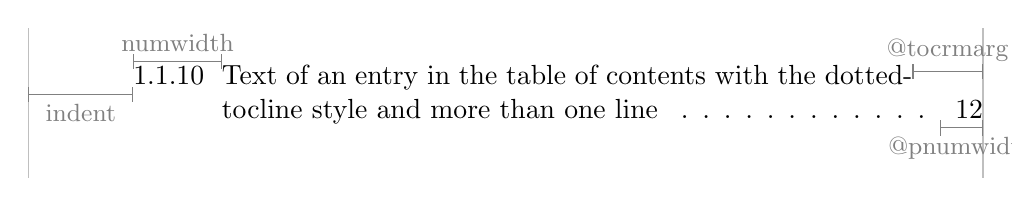
\begin{tikzpicture}
        \draw[color=lightgray] (0,2\baselineskip) -- (0,-2.5\baselineskip);
        \draw[color=lightgray] (\linewidth,2\baselineskip) --
                               (\linewidth,-2.5\baselineskip);
        \node (dottedtocline) at (0,0) [anchor=west,inner sep=0,outer sep=0]
        {%
          \hspace*{7em}%
          \parbox[t]{\dimexpr\linewidth-9.55em}{%
            \setlength{\parindent}{-3.2em}%
            \addtolength{\parfillskip}{-2.55em}%
            \makebox[3.2em][l]{1.1.10}%
            Text of an entry in the table of contents with the
            \PValue{dottedtocline} style and more than one line%
            \leaders\hbox{$\csname m@th\endcsname
              \mkern 4.5mu\hbox{.}\mkern 4.5mu$}\hfill\nobreak
            \makebox[1.55em][r]{12}%
          }%
        };
        \draw[|-|,color=gray,overlay] (0,0) --
                              node [anchor=north,font=\small] {
                                \PValue{indent}
                              }
                              (3.8em,0);
        \draw[|-|,color=gray,overlay] (3.8em,\baselineskip) -- 
                              node [anchor=south,font=\small] {
                                \PValue{numwidth}
                              }
                              (7em,\baselineskip);
        \draw[|-|,color=gray,overlay] (\linewidth,\ht\strutbox) -- 
                              node [anchor=south,font=\small] { 
                                \Macro{@tocrmarg} 
                              }
                              (\linewidth-2.55em,\ht\strutbox);
        \draw[|-|,color=gray,overlay] (\linewidth,-\baselineskip) -- 
                              node [anchor=north,font=\small] { 
                                \Macro{@pnumwidth} 
                              } 
                              (\linewidth-1.55em,-\baselineskip);
      \end{tikzpicture}%
    }
    \caption{Illustrations of some attributes of a TOC entry with the
      \PValue{dottedtocline} style}
    \label{fig:tocbasic.dottedtocline}
  \end{figure}
\item[\PValue{gobble}] is the simplest possible style. Entries in this style,
  regardless of the setting of \DescRef{\LabelBase.counter.tocdepth}%
  \IndexCounter{tocdepth}\important{\DescRef{\LabelBase.counter.tocdepth}},
  will never be printed. The style simply gobbles the
  entries, so to speak. It has the default \PValue{level} attribute, but
  it is never evaluated.
\item[\PValue{largetocline}] is similar to the style used by the standard
  classes for the \PValue{part} level. It supports the \PValue{level} and
  \PValue{indent} attributes only. The latter deviates from the standard
  classes, which do not support an indent of the \PValue{part} entries.

  A penalty is set to permit page breaks before an entry of an appropriate
  level. The entries will be indented by the value of \PValue{indent} from the
  left and printed with the font style \Macro{large}\Macro{bfseries}. If
  \DescRef{\LabelBase.cmd.numberline} is used, the number width is 3\Unit{em}.
  \DescRef{\LabelBase.cmd.numberline} is not redefined. The standard classes
  do not use \DescRef{\LabelBase.cmd.numberline} for \PName{part} entries. The
  value of \PName{indent} also has no effect on the indentation from the
  second line and after in a multi-line entry.

  \hyperref[fig:tocbasic.largetocline]%
  {Figure~\ref*{fig:tocbasic.largetocline}} illustrates the characteristics of
  this style. You will also notice that the style has adopted some
  inconsistencies present in the standard classes, e.\,g. the missing indent
  of the second and following lines of an entry or the different values of
  \Macro{@pnumwidth} that results from the font-size dependency. This can
  result, in extreme cases, in the entry text coming too close. Note that the
  width of the entry number shown in the figure is only valid if
  \DescRef{\LabelBase.cmd.numberline} has been used. The standard classes,
  however, use a distance of 1\Unit{em} after the number.
  \begin{figure}
    \centering
    \resizebox{.8\linewidth}{!}{%
      
\begin{tikzpicture}
        \draw[color=lightgray] (0,2\baselineskip) -- (0,-2.5\baselineskip);
        \draw[color=lightgray] (\linewidth,2\baselineskip) --
                               (\linewidth,-2.5\baselineskip);
        \node (largetocline) at (0,0) [anchor=west,inner sep=0,outer sep=0] {%
          \parbox[t]{\dimexpr \linewidth-1.55em\relax}{%
            \makebox[3em][l]{\large\bfseries I}%
            \large\bfseries
            Text of an entry to the table of contents with the
            \PValue{largetocline} style and more than one line%
            \hfill
            \makebox[0pt][l]{\normalsize\normalfont
              \makebox[1.55em][r]{\large\bfseries 1}}%
          }%
        };
        \draw[|-|,color=gray] (0,\baselineskip) -- 
                              node [anchor=south] { 3\,em } 
                              (3em,\baselineskip);
        \draw[|-|,color=gray,overlay] (\linewidth,\ht\strutbox) -- 
                              node [anchor=south] { \Macro{@pnumwidth} }
                              (\linewidth-1.55em,\ht\strutbox);
        \large\bfseries
        \draw[|-|,color=gray,overlay] (\linewidth,-\baselineskip) -- 
                              node [anchor=north,font=\normalfont\normalsize] { 
                                \Macro{large}\Macro{@pnumwidth} 
                              }
                              (\linewidth-1.55em,-\baselineskip);
      \end{tikzpicture}%
    }
    \caption{Illustrations of some attributes of a TOC entry with style 
      \PValue{largetocline}}
    \label{fig:tocbasic.largetocline}
  \end{figure}
\item[\PValue{tocline}] is a flexible style. The \KOMAScript{} classes use
  this style by default for all kinds of entries. Likewise, these classes
  define the clones \PValue{part}, \PValue{chapter}, and \PValue{section}, or
  \PValue{section} and \PValue{subsection} using this style, but add extra
  \PName{initial code} to the clones to change their defaults.

  The style supports 18\important{\PValue{level}, \PValue{beforeskip},
    \PValue{breakafternumber}, \PValue{dynnumwidth}, \PValue{entryformat},
    \PValue{entrynumberformat}, \PValue{indent}, \PValue{linefill},
    \PValue{numsep}, \PValue{numwidth}, \PValue{onstarthigherlevel},
    \PValue{onstartlowerlevel}, \PValue{onstartsamelevel},
    \PValue{pagenumberbox}, \PValue{pagenumberformat},
    \PValue{pagenumberwidth}, \PValue{raggedentrytext},
    \PValue{raggedpagenumber}, \PValue{rightindent}} additional attributes in
  addition to the default \PValue{level} attribute. The defaults of all these
  attributes depend on the name of the \PName{entry level} and correspond to
  the results of the standard classes. So after loading \Package{tocbasic},
  you can change the style of the entries in the table of contents of the
  standard classes into \PValue{tocline} using
  \DescRef{\LabelBase.cmd.DeclareTOCEntryStyle} without this leading directly
  to major changes in their appearance. Thus you can precisely change only
  those attributes that are necessary for the desired changes. The same
  applies to the list of figures and the list of tables for the standard
  classes.

  Because its great flexibility, this style can in principle replace the
  \PValue{dottedtocline}, \PValue{undottedtocline}, and \PValue{largetocline}
  styles, but this requires more effort to configure.

  \hyperref[fig:tocbasic.tocline]%
  {Figure~\ref*{fig:tocbasic.tocline}} illustrates some of the length
  attributes of this style. The others are explained in
  \autoref{tab:tocbasic.tocstyle.attributes} starting on
  \autopageref{tab:tocbasic.tocstyle.attributes}.
  \begin{figure}
    \centering
    \resizebox{.8\linewidth}{!}{%
      \begin{tikzpicture}
        \coordinate (subsection) at (0,0);
        \coordinate (section) at ($(subsection)+(0,2\baselineskip)$);
        \coordinate (chapter) at ($(section)+(0,2\baselineskip)$);
        \coordinate (part)    at ($(chapter)+(0,2.4\baselineskip+1em)$);

        \draw[color=lightgray] 
          ($(part)+(0,2\baselineskip)$) -- 
          (0,-2.5\baselineskip);
        \draw[color=lightgray] 
          ($(part)+(\linewidth,2\baselineskip)$) --
          (\linewidth,-2.5\baselineskip);

        \coordinate (subsection) at (0,0);

        \node at (part) [anchor=west,inner sep=0,outer sep=0]
        {%
          \hspace*{3em}%
          \parbox[t]{\dimexpr\linewidth-5.55em}{%
            \setlength{\parindent}{-3em}%
            \addtolength{\parfillskip}{-2.55em}%
            \makebox[3em][l]{\large\bfseries I.}%
            \textbf{\large Text of a part entry with the
            \PValue{tocline} style and at least two lines of text}%
            \hfill
            \makebox[1.55em][r]{\bfseries 12}\large
          }%
        };
        \draw[|-|,color=gray,overlay] 
          (part) --
          ($(part)+(3em,0)$)
          node [anchor=north east,font=\small] {
            \PValue{numwidth}
          };
        \draw[|-|,color=gray,overlay] 
          ($(part)+(\linewidth,\ht\strutbox)$)
          node [anchor=north,font=\small] { 
            \Macro{@tocrmarg} 
          } --
          ($(part)+(\linewidth-2.55em,\ht\strutbox)$);
        \draw[|-|,color=gray,overlay] 
          ($(part)+(\linewidth,-\baselineskip)$) -- 
          node [anchor=north,font=\small] { 
            \Macro{@pnumwidth} 
          } 
          ($(part)+(\linewidth-1.55em,-\baselineskip)$);
        \node at (chapter) [anchor=west,inner sep=0,outer sep=0]
        {%
          \hspace*{1.5em}%
          \parbox[t]{\dimexpr\linewidth-4.05em}{%
            \setlength{\parindent}{-1.5em}%
            \addtolength{\parfillskip}{-2.55em}%
            \makebox[1.5em][l]{\bfseries 1.}%
            \textbf{Text of a chapter entry with the
            \PValue{tocline} style and more than one line of text
            for demonstration purposes}%
            \hfill
            \makebox[1.55em][r]{\bfseries 12}%
          }%
        };
        \draw[|-|,color=gray,overlay]
          ($(chapter)+(3em,\baselineskip)$) --
          node [anchor=west,font=\small] {
            \PValue{beforeskip}
          }
          ($(part)+(3em,-\baselineskip)$);
        \draw[|-|,color=gray,overlay] 
          (chapter) --
          ($(chapter)+(1.5em,0)$)
          node [anchor=north east,font=\small] {
            \PValue{numwidth}
          };
        \draw[|-|,color=gray,overlay] 
          ($(chapter)+(\linewidth,\ht\strutbox)$)
          node [anchor=north,font=\small] { 
            \Macro{@tocrmarg} 
          } --
          ($(chapter)+(\linewidth-2.55em,\ht\strutbox)$);
        \draw[|-|,color=gray,overlay] 
          ($(chapter)+(\linewidth,-\baselineskip)$)
          node [anchor=north,font=\small] { 
            \Macro{@pnumwidth} 
          } --
          ($(chapter)+(\linewidth-1.55em,-\baselineskip)$);
        \node at (section) [anchor=west,inner sep=0,outer sep=0]
        {
          \hspace*{3.8em}%
          \parbox[t]{\dimexpr\linewidth-6.35em}{%
            \setlength{\parindent}{-2.3em}%
            \addtolength{\parfillskip}{-2.55em}%
            \makebox[2.3em][l]{1.1.}%
            Text of a section entry with the \PValue{tocline}
            style and more than one line of text for
            demonstration purposes%
            \leaders\hbox{$\csname m@th\endcsname
              \mkern 4.5mu\hbox{.}\mkern 4.5mu$}\hfill\nobreak
            \makebox[1.55em][r]{3}%
          }%
        };
        \node at (subsection) [anchor=west,inner sep=0,outer sep=0]
        {%
          \hspace*{7em}%
          \parbox[t]{\dimexpr\linewidth-9.55em}{%
            \setlength{\parindent}{-3.2em}%
            \addtolength{\parfillskip}{-2.55em}%
            \makebox[3.2em][l]{1.1.10.}%
            Text of a subsection entry with the \PValue{tocline}
            and more than one line of text for demonstration
            purposes%
            \leaders\hbox{$\csname m@th\endcsname
              \mkern 4.5mu\hbox{.}\mkern 4.5mu$}\hfill\nobreak
            \makebox[1.55em][r]{12}%
          }%
        };
        \draw[|-|,color=gray,overlay] 
          ($(subsection)+(0,\ht\strutbox)$) -- 
          node [anchor=north,font=\small] {
            \PValue{indent}
          }
          ($(subsection)+(3.8em,\ht\strutbox)$);
        \draw[|-|,color=gray,overlay] 
          ($(subsection)+(3.8em,0)$) --
          ($(subsection)+(7em,0)$)
          node [anchor=north east,font=\small] {
            \PValue{numwidth}
          };
        \draw[|-|,color=gray,overlay] 
          ($(subsection)+(\linewidth,\ht\strutbox)$)
          node [anchor=north,font=\small] { 
            \Macro{@tocrmarg} 
          } --
          ($(subsection)+(\linewidth-2.55em,\ht\strutbox)$);
        \draw[|-|,color=gray,overlay] 
          ($(subsection)+(\linewidth,-\baselineskip)$) -- 
          node [anchor=north,font=\small] { 
            \Macro{@pnumwidth} 
          } 
          ($(subsection)+(\linewidth-1.55em,-\baselineskip)$);
      \end{tikzpicture}%
    }
    \caption{Illustrations of some attributes of a TOC entry with the
      \PValue{tocline} style}
    \label{fig:tocbasic.tocline}
  \end{figure}
\item[\PValue{toctext}]\ChangedAt{v3.27}{\Package{tocbasic}}%
  is a special feature. While all other styles produce one paragraph per
  entry, this one produces one paragraph for all successive entries of this
  style. With 13\important{\PValue{afterpar}, \PValue{entryformat},
    \PValue{entrynumberformat}, \PValue{indent}, \PValue{numsep},
    \PValue{onendentry}, \PValue{onendlastentry}, \PValue{onstartentry},
    \PValue{onstartfirstentry}, \PValue{pagenumberformat},
    \PValue{prepagenumber}, \PValue{raggedright}, \PValue{rightindent}}
  attributes in addition to the default \PValue{level} attribute, there are
  almost as many options as for \PValue{tocline}. However, this style
  depends on the fact that an unfinished paragraph will be concluded at the
  beginning of the entry for all other styles, as well as at the end of the
  current content list. So it should never be combined with entries or content
  lists that are generated outside of \Package{tocbasic}.
\item[\PValue{undottedtocline}] is similar to the style used by the standard
  \Class{book} and \Class{report} classes for the \PValue{chapter} entry
  level, or by \Class{article} for the \PValue{section} entry level in the
  table of contents. It supports\important{\PValue{level}, \PValue{indent},
  \PValue{numwidth}} only three attributes. A penalty is inserted permitting
  an appropriate page break before the entry, as is a vertical skip. The
  entries are printed with an indentation of \PValue{indent} from the left and
  in \Macro{bfseries}. This is a departure from the standard classes, which do
  not support the indentation of these entry levels.
  \DescRef{\LabelBase.cmd.numberline} is used unchanged. The width of the
  entry number is determined by \PValue{numwidth}. For multi-line entries the
  indent will be increased by the value of \PValue{numwidth} for the second
  and following lines. \hyperref[fig:tocbasic.undottedtocline]%
  {Figure~\ref*{fig:tocbasic.undottedtocline}} illustrates the attributes of
  this style.
  \begin{figure}
    \centering
    \resizebox{.8\linewidth}{!}{%
      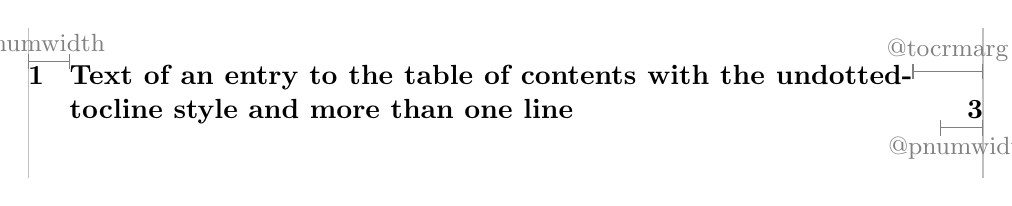
\begin{tikzpicture}
        \draw[color=lightgray] (0,2\baselineskip) -- (0,-2.5\baselineskip);
        \draw[color=lightgray] (\linewidth,2\baselineskip) --
                               (\linewidth,-2.5\baselineskip);
        \node (undottedtocline) at (0,0) [anchor=west,inner sep=0,outer sep=0]
        {%
          \makebox[1.5em][l]{\bfseries 1}%
          \parbox[t]{\dimexpr \linewidth-4.05em\relax}{%
            \bfseries
            Text of an entry to the table of contents with the
            \PValue{undottedtocline} style and more than one line%
          }%
          \raisebox{-\baselineskip}{\makebox[2.55em][r]{\bfseries 3}}%
        };
        \draw[|-|,color=gray,overlay] (0,\baselineskip) -- 
                              node [anchor=south,font=\small] {
                                \PValue{numwidth}
                              }
                              (1.5em,\baselineskip);
        \draw[|-|,color=gray,overlay] (\linewidth,\ht\strutbox) -- 
                              node [anchor=south,font=\small] { 
                                \Macro{@tocrmarg} 
                              }
                              (\linewidth-2.55em,\ht\strutbox);
        \draw[|-|,color=gray,overlay] (\linewidth,-\baselineskip) -- 
                              node [anchor=north,font=\small] { 
                                \Macro{@pnumwidth} 
                              } 
                              (\linewidth-1.55em,-\baselineskip);
      \end{tikzpicture}%
    }
    \caption{Illustration of some attributes of the \PValue{undottedtocline}
      style with the example of a chapter title}%
    \label{fig:tocbasic.undottedtocline}
  \end{figure}
\end{description}
You can find an explanation of the attributes of all styles that
\Package{tocbasic} defines in \autoref{tab:tocbasic.tocstyle.attributes}.
In\ChangedAt{v3.27}{\Package{tocbasic}} addition to the usual assignment with
\Option{\PName{key}=\PName{value}}, both commands understand an assignment in 
the form \Option{\PName{key}:=\PName{entry level}} for all options of the
\KOMAScript{} styles. In this case, the current setting of \PName{key} for the
\PName{entry level} will be copied. For example, you can copy the current
indent of the \PValue{figure} level using \OptionValue{indent:}{figure}. For
options that expect a length or integer value, you can also use
\Option{\PName{key}+=\PName{value}} to add\PName{value} to the current setting
of the \PName{key}. To subtract simply, you can use a negative \PName{value}.
For example, with \OptionValue{indent+}{1cm} you can increase the indent by
1\Unit{cm}.

If\ChangedAt{v3.21}{\Package{tocbasic}} you use these attributes as
options to \DescRef{\LabelBase.cmd.DeclareNewTOC} (see
\DescPageRef{\LabelBase.cmd.DeclareNewTOC}), you must prefix the names of the
attributes with \PValue{tocentry}, e\,g., \PValue{level} becomes
\Option{tocentrylevel}. The copy operation with \Option{:=} described above is
also available here. However, addition with \Option{+=} is not currently
supported.

If\ChangedAt{v3.20}{\Package{tocbasic}} you use
these attributes as options for
\DescRef{maincls-experts.cmd.DeclareSectionCommand}%
\IndexCmd{DeclareSectionCommand}\IndexCmd{DeclareNewSectionCommand}%
\IndexCmd{RedeclareSectionCommand}\IndexCmd{ProvideSectionCommand} (see
\DescPageRef{maincls-experts.cmd.DeclareSectionCommand}) and similar commands,
you must prefix the names of the attributes with \PValue{toc}, e\,g.
\PValue{level} becomes \Option{toclevel}.
At this time, neither the copy operation with \Option{:=} nor the
addition operation with \Option{+=} is supported.

Finally, using \Macro{DeclareTOCStyleEntry} will define the internal command
\Macro{l@\PName{entry level}}.

\begin{desclist}
  \desccaption{%
    Attributes of the predefined TOC-entry styles of \Package{tocbasic}%
    \label{tab:tocbasic.tocstyle.attributes}%
  }{%
    Attributes of the TOC-entry styles (\emph{continued})%
  }%
  \entry{\OptionVName{afterpar}{code}}{%
    \ChangedAt{v3.27}{\Package{tocbasic}}%
    The specified \PName{code} will be executed after the end of the paragraph
    in which an entry with the \PValue{toctext} style is printed. If several
    entries have such settings, their code will be executed in the order of
    the entries.%
  }%
  \entry{\OptionVName{beforeskip}{length}}{%
    The  vertical distance inserted before an entry of this level in the
    \PValue{tocline} style (see \autoref{fig:tocbasic.tocline}). The distance
    is made using either \Macro{vskip} or \Macro{addvspace} depending on the
    \PName{entry level}, to maintain compatibility as far as possible with the
    standard classes and earlier versions of \KOMAScript.

    For the \PValue{part} \PName{entry level}, the attribute will be
    initialised with \texttt{2.25em plus 1pt}; for \PValue{chapter}, with
    \texttt{1em plus 1pt}. If the \PName{chapter} \PName{entry level} is
    undefined, \PValue{section} is initialised with \texttt{1em plus 1pt}
    instead. The initial value for all other levels is \texttt{0pt plus
      .2pt}.%
  }%
  \entry{\OptionVName{breakafternumber}{switch}}{%
    \PName{switch} is one of the values for simple switches from
    \autoref{tab:truefalseswitch}, \autopageref{tab:truefalseswitch}. If the
    switch is active in the \PValue{tocline} style, there will be a line break
    after the number set with
    \DescRef{\LabelBase.cmd.numberline}\IndexCmd{numberline}. The line after
    the entry number again starts flush left with the number. The default is
    false for the \PValue{tocline} style.

    If\textnote{Attention!} the \Option{numberline} feature has been activated
    for a content list  (see \DescRef{\LabelBase.cmd.setuptoc},
    \autoref{sec:tocbasic.toc}, \DescPageRef{\LabelBase.cmd.setuptoc}), as is
    the case with the \KOMAScript{} classes when the
    \OptionValueRef{maincls}{toc}{numberline}%
    \IndexOption{toc~=\textKValue{numberline}} option is used, then the
    unnumbered entries will nevertheless have a (by default empty) number line
    using the formatting of \Option{entrynumberformat}.%
  }%
  \entry{\OptionVName{dynnumwidth}{switch}}{%
    \PName{switch} is one of the values for simple switches from
    \autoref{tab:truefalseswitch}, \autopageref{tab:truefalseswitch}. If the
    switch is active with the \PValue{tocline} style, the \PValue{numwidth}
    attribute specifies a minimum value. If a previous \LaTeX{} run has
    determined that the maximum width of the entry numbers of the same level
    plus the value of \PValue{numsep} is greater than this minimum, the
    calculated value will be used instead.%
  }%
  \entry{\OptionVName{entryformat}{command}}{%
    You can use this attributes to change the format of the entry. The value
    should be a \PName{command} with exactly one argument. This argument is
    not necessarily fully expandable. You should not use commands like
    \Macro{MakeUppercase}, which expects a fully expandable argument. Font
    changes are relative to \Macro{normalfont}\Macro{normalsize}. Note that
    the output of \Option{linefill} and the page number are independent of
    \Option{entryformat}. See also the \Option{pagenumberformat} attribute .

    The initial value of the attribute for the \PValue{part} \PName{entry
    level} is \Macro{large}\Macro{bfseries}, and for \PValue{chapter}, it is
    \Macro{bfseries}. If the \PValue{chapter} level is not defined,
    \PValue{section} uses \Macro{bfseries}. All other levels print the
    argument unchanged.%
  }%
  \entry{\OptionVName{entrynumberformat}{command}}{%
    You can use this attribute to format the entry number within
    \DescRef{\LabelBase.cmd.numberline}. The value should be a \PName{command}
    with exactly one argument. Font changes are relative to the one of
    attribute \Option{entryformat}.

    The initial \PName{command} prints the argument unchanged. This means the
    entry number will be printed as it is.

    If\textnote{Attention!} the \Option{numberline} feature for a content list
    has been activated (see \DescRef{\LabelBase.cmd.setuptoc},
    \autoref{sec:tocbasic.toc}, \DescPageRef{\LabelBase.cmd.setuptoc}), as is
    the case with the \KOMAScript{} classes using the
    \OptionValueRef{maincls}{toc}{numberline}%
    \IndexOption{toc~=\textKValue{numberline}} option, the unnumbered entries
    will execute the \PName{command} as well.%
  }%
  \entry{%
    \OptionVName{indent}{length}%
    {\phantomsection\label{tab:tocbasic.tocstyle.attributes.indent}}%
  }{%
    For\ChangedAt{v3.27}{\Package{tocbasic}} the \PValue{toctext} style, the
    \PName{length} is the horizontal distance of the paragraph from the left
    margin. If different entries within the paragraph have different settings,
    the last one is used. For the remaining styles, the \PName{length} is the
    horizontal distance of the entry from the left margin (see
    \autoref{fig:tocbasic.dottedtocline} and \autoref{fig:tocbasic.tocline}).
    
    For the styles \PValue{tocline} and \PValue{toctext}, all entry levels
    whose names start with ``\texttt{sub}'' are initialised with the
    \PValue{indent}+\PValue{numwidth} of the entry level of the same name
    without this prefix. For the \PValue{dottedtocline},
    \PValue{undottedtocline}, and \PValue{tocline} styles, the initial values
    of levels \PValue{part} down to \PValue{subparagraph} and the levels
    \PValue{figure} and \PValue{table} are compatible with the standard
    classes. All other levels do not have an initial value. Therefore you have
    to set an explicit value for such levels when they are defined first
    time.

    If the \PValue{noindent} attribute is set for a content list via
    \DescRef{\LabelBase.cmd.setuptoc}, the entries of all styles provided by
    \KOMAScript{} enforce the value 0\Unit{pt} to deactivate the indent.%
  }%
  \entry{\OptionVName{level}{integer}}{%
    The numerical value of the \PName{entry level}. Only those entries whose
    numerical value is less than or equal to the
    \DescRef{\LabelBase.counter.tocdepth}%
    \important{\DescRef{\LabelBase.counter.tocdepth}}\IndexCounter{tocdepth}
    counter are printed.

    This attribute is mandatory for all styles and will be defined
    automatically when the style is declared.

    For the \PValue{tocline} and \PValue{toctext} styles, all entry levels
    whose name starts with ``\texttt{sub}'' are initialised with the value of
    the entry level of the same name without this prefix plus one. For the
    \PValue{dottedtocline}, \PValue{largetocline}, \PValue{tocline},
    \PValue{toctext}, and \PValue{undottedtocline} styles, the entry levels
    from \PValue{part} to \PValue{subparagraph}, as well as \PValue{figure}
    and \PValue{table}, are initialised to be compatible with the standard
    classes. For all other levels, the initialisation is done with the value
    of \Macro{\PName{entry level}numdepth}, if this is defined.%
  }%
  \entry{\OptionVName{linefill}{code}}{%
    With the \PValue{tocline} style, you can change what is used to fill the
    space between the end of the entry text and the page number. The
    \PName{linefill} attribute contains the \PName{code} that prints this
    filler. For the \PValue{part} and \PValue{chapter} \PName{entry level}s,
    the attribute is initialised with \Macro{hfill}. If no \PValue{chapter}
    \PName{entry level} has been defined, \PValue{section} also uses
    \Macro{hfill}. All other entry levels are initialised with
    \DescRef{\LabelBase.cmd.TOCLineLeaderFill} (see
    \DescPageRef{\LabelBase.cmd.TOCLineLeaderFill}).

    Incidentally, if the \PName{code} specified does not automatically fill
    the gap, you should also activate the \PValue{raggedpagenumber} attribute 
    to avoid ``\texttt{underfull \Macro{hbox}}'' messages.%
  }%
  \entry{\OptionVName{numsep}{length}}{%
    The \PValue{tocline} style tries to ensure a minimum distance of
    \PName{length} between the entry number and the entry text. If
    \PValue{dynnumwidth} is active, it will correct the number width to
    achieve this. Otherwise it simply throws a warning if the condition is not
    met.

    The\ChangedAt{v3.27}{\Package{tocbasic}} \PValue{toctext} style, on the
    other hand, always adds a horizontal space of width \PName{length} after
    the number of the entry.
    
    The initial \PName{length} is 0.4\Unit{em}.%
  }%
  \entry{\OptionVName{numwidth}{length}}{%
    The width reserved for the entry number (see
    \autoref{fig:tocbasic.dottedtocline} to
    \autoref{fig:tocbasic.undottedtocline}). With the \PValue{dottedtocline},
    \PValue{tocline}, and \PValue{undottedtocline} styles, this \PName{length}
    is added to the \PName{length} of attribute \PValue{indent} for the second
    and following lines of the entry text.

    With the \PValue{tocline} style, the initial \PName{length} of all entries
    whose name starts with ``\texttt{sub}'' is the value of the level without
    this prefix plus 0.9\Unit{em}, if such a level with corresponding
    attributes exists. With the \PValue{dottedtocline},
    \PValue{undottedtocline}, and \PValue{tocline} styles, the initial
    \PName{length}s of levels from \PValue{part} to \PValue{subparagraph}, as
    well as \PName{figure} and \PName{table}, are compatible with those of the
    standard classes. All other levels do not have an initial value. Therefore
    you must set \PValue{numwidth} explicitly when the entry level is first
    used.%
  }%
  \entry{\OptionVName{onendentry}{code}}{%
    \ChangedAt{v3.27}{\Package{tocbasic}}%
    The \PName{code} is executed immediately after an entry with the
    \PValue{toctext} style, if this entry is not the last one of the
    paragraph. The user must ensure that the \PName{code} does not result in
    the paragraph ending.

    Note: In reality the \PName{code} is not executed at the end of the entry
    but before the next entry with style \PValue{toctext}.%
  }%
  \entry{\OptionVName{onendlastentry}{code}}{%
    \ChangedAt{v3.27}{\Package{tocbasic}}%
    The \PName{code} is executed immediately before the end of the paragraph
    with an entry in the \PValue{toctext} style, as long as this entry is the
    last one in the paragraph. The user must ensure that the \PName{code} does
    not result in the paragraph ending.%
  }%
  \entry{\OptionVName{onstartentry}{code}}{%
    \ChangedAt{v3.27}{\Package{tocbasic}}%
    The \PName{code} is executed immediately before an entry with the
    \PValue{toctext} style, unless it is the first one in the paragraph. The
    user must ensure that the \PName{code} does not result in the paragraph
    ending.%
  }%
  \entry{\OptionVName{onstartfirstentry}{code}}{%
    \ChangedAt{v3.27}{\Package{tocbasic}}%
    The \PName{code} is executed immediately before an entry with the
    \PValue{toctext} style if this entry is the first one of the paragraph. The
    user must ensure that the \PName{code} does not result in the paragraph
    ending.%
  }%
  \entry{\OptionVName{onstarthigherlevel}{code}}{%
    The \PValue{tocline} style can execute \PName{code} at the start of an
    entry, depending on whether the previous entry had numerical level greater
    than, the same as, or less than the current entry. The \PName{code}
    specified by this attribute will be executed if the current entry has a
    greater numerical value, i.\,e. it is lower in the entry hierarchy, than
    the previous one.

    Note that detecting the level of the previous entry only works so long as
    \Macro{lastpenalty} has not changed since the previous entry.

    The initial \PName{code} is \DescRef{\LabelBase.cmd.LastTOCLevelWasLower}
    (see \DescPageRef{\LabelBase.cmd.LastTOCLevelWasLower}).%
  }%
  \entry{\OptionVName{onstartlowerlevel}{code}}{%
    The \PValue{tocline} style can execute \PName{code} at the start of an
    entry, depending on whether the previous entry had numerical level greater
    than, the same as, or less than the current entry. The \PName{code}
    specified by this attribute will be executed if the current entry has a
    lower numerical value, i.\,e. it is higher in the entry hierarchy, than
    the previous one.

    Note that detecting the level of the previous entry only works so long as
    \Macro{lastpenalty} has not changed since the previous entry.

    The initial \PName{code} is \DescRef{\LabelBase.cmd.LastTOCLevelWasHigher}
    (see \DescPageRef{\LabelBase.cmd.LastTOCLevelWasHigher}), which usually
    favours a page break before the entry.%
  }%
  \entry{\OptionVName{onstartsamelevel}{code}}{%
    The \PValue{tocline} style can execute \PName{code} at the start of an
    entry, depending on whether the previous entry had numerical level greater
    than, the same as, or less than the current entry. The \PName{code}
    specified by this attribute will be executed if the current entry has the
    same numerical value, i.\,e. it is on the same level in the entry
    hierarchy, as the previous one.

    Note that detecting the level of the previous entry only works so long as
    \Macro{lastpenalty} has not changed since the previous entry.

    The initial \PName{code} is \DescRef{\LabelBase.cmd.LastTOCLevelWasSame}
    (see \DescPageRef{\LabelBase.cmd.LastTOCLevelWasSame}), which usually
    favours a page break before the entry.%
  }%
  \entry{\OptionVName{pagenumberbox}{command}}{%
    By default the page number of an entry is printed flush right in a box
    of width \Macro{@pnumwidth}. In the \PValue{tocline} style, you can
    change the \PName{command} to print the number using this attribute. The
    \PName{command} should expect exactly one argument, the page number.
    
    This attribute is initialised with the box already mentioned.%
  }%
  \entry{\OptionVName{pagenumberformat}{command}}{%
    You can use this attribute to change the format of the page number of an
    entry. The \PName{command} should expect exactly one argument, the page
    number. Font changes are relative to the font of \Option{entryformat}
    followed by \Macro{normalfont}\Macro{normalsize}.

    The initial \PName{command} of entry level \PValue{part} prints the
    argument in \Macro{large}\Macro{bfseries}. The initial \PName{command} of
    all other levels prints the argument in
    \Macro{normalfont}\Macro{normalcolor}.%
  }%
  \entry{\OptionVName{pagenumberwidth}{length}}{%
    \ChangedAt{v3.27}{\Package{tocbasic}}%
    You can use this attribute to locally change the width of the default box
    for the page number of an entry with the style \PValue{tocline} from
    \Macro{@pnumwidth} to the specified \PName{length}. Note that if you
    change the default page number box with the \Option{pagenumberbox}
    attribute, the specified \PName{length} will no longer be used
    automatically.%
  }%
  \entry{\OptionVName{prepagenumber}{code}}{%
    \ChangedAt{v3.27}{\Package{tocbasic}}%
    The \PValue{toctext} style executes the \PName{code} between the text and
    the page number of the entry. Usually this is used to add a horizontal
    space or separator between text and page number.%

    The default is a non-breaking space using \Macro{nonbreakspace}.%
  }%
  \entry{\OptionVName{raggedentrytext}{switch}}{%
    The\ChangedAt{v3.21}{\Package{tocbasic}} \PName{switch} is one of the
    values for simple switches from \autoref{tab:truefalseswitch},
    \autopageref{tab:truefalseswitch}. If the switch is active, the
    \PValue{tocline} style prints the text of an entry ragged right instead of
    fully justified, and only words that are longer than a text line are
    automatically hyphenated.

    This \PName{switch} is false by default.%
  }%
 \entry{\OptionVName{raggedpagenumber}{switch}}{%
    The \PName{switch} is one of the values for simple switches from
    \autoref{tab:truefalseswitch}, \autopageref{tab:truefalseswitch}. If the
    switch is active, the \PValue{tocline} style does not force the page
    number to be right justified.

    Depending on the value of \PValue{linefill}, setting this attribute could
    affect only whether a warning message appears, or the formatting of the
    page number as well. So it is important to set both attributes so that
    they correspond.

    By default the \PName{switch} is not activated and therefore corresponds
    with an initial value of \Macro{hfill} or
    \DescRef{\LabelBase.cmd.TOCLineLeaderFill} for the \PValue{linefill}
    attribute.%
  }%
  \entry{\OptionVName{raggedright}{switch}}{%
    \ChangedAt{v3.27}{\Package{tocbasic}}%
    The \PName{switch} is one of the values for simple switches from
    \autoref{tab:truefalseswitch}, \autopageref{tab:truefalseswitch}. If the
    switch is active for any entry with the \PValue{toctext} style inside the
    same paragraph, the whole paragraph is printed ragged right.
  }%
  \entry{\OptionVName{rightindent}{length}}{%
    \ChangedAt{v3.27}{\Package{tocbasic}}%
    You can use this attribute to locally change the right indent for the text
    of an entry with the \PValue{tocline} style from \Macro{@tocrmarg} to the
    specified \PName{length}.%
  }%
\end{desclist}

While \Macro{DeclareTOCStyleEntry} defines only one \PName{entry level},
\Macro{DeclareTOCStyleEntries}\ChangedAt{v3.26}{\Package{tocbasic}} can define
an entire list of \PName{entry level}s in one command. Each entry level in the
comma-separated \PName{entry-level list} is defined with the same \PName{style}
and settings of the given \PName{option list}.%
\EndIndexGroup


\begin{Declaration}
  \Macro{DeclareTOCEntryStyle}\Parameter{style}%
                              \OParameter{initial code}%
                              \Parameter{command code}%
  \Macro{DefineTOCEntryOption}\Parameter{option}\OParameter{default value}%
                              \Parameter{code}%
  \Macro{DefineTOCEntryBooleanOption}\Parameter{option}%
                                     \OParameter{default value}%
                                     \Parameter{prefix}%
                                     \Parameter{postfix}%
                                     \Parameter{description}%%
                                     %\OParameter{initial code}%
  \Macro{DefineTOCEntryCommandOption}\Parameter{option}%
                                     \OParameter{default value}%
                                     \Parameter{prefix}%
                                     \Parameter{postfix}%
                                     \Parameter{description}%%
                                     %\OParameter{initial code}%
  \Macro{DefineTOCEntryIfOption}\Parameter{option}%
                                     \OParameter{default value}%
                                     \Parameter{prefix}%
                                     \Parameter{postfix}%
                                     \Parameter{description}%%
                                     %\OParameter{initial code}%
  \Macro{DefineTOCEntryLengthOption}\Parameter{option}%
                                     \OParameter{default value}%
                                     \Parameter{prefix}%
                                     \Parameter{postfix}%
                                     \Parameter{description}%%
                                     %\OParameter{initial code}%
  \Macro{DefineTOCEntryNumberOption}\Parameter{option}%
                                     \OParameter{default value}%
                                     \Parameter{prefix}%
                                     \Parameter{postfix}%
                                     \Parameter{description}%
                                     %\OParameter{initial code}%
\end{Declaration}
\Macro{DeclareTOCEntryStyle}\ChangedAt{v3.20}{\Package{tocbasic}} is
one of the most complex commands in \KOMAScript. It is therefore explicitly
intended for \LaTeX{} developers and not for ordinary \LaTeX{} users. It lets
you define new a \PName{style} for content-list entries. Usually, entries to
content lists are made using
\Macro{addcontentsline}\IndexCmd{addcontentsline}, or preferably, if you use
\Package{tocbasic}, with
\DescRef{\LabelBase.cmd.addxcontentsline}\IndexCmd{addxcontentsline} (see
\autoref{sec:tocbasic.basics}, \DescPageRef{\LabelBase.cmd.addxcontentsline}).
In both cases \LaTeX{} writes a corresponding
\Macro{contentsline}\IndexCmd{contentsline} to the appropriate auxiliary file.
When reading this auxiliary file, \LaTeX{} then executes a
\Macro{l@\PName{entry level}} command for each \Macro{contentsline}.

If you later assign a \PName{style} to an entry level using
\DescRef{\LabelBase.cmd.DeclareTOCStyleEntry}, the \PName{initial code} is
executed first, if provided, and then the \PName{command code} for the
definition of \Macro{l@\PName{entry level}}. The \PName{command code} is the
code that will be expanded and executed by \Macro{l@\PName{entry level}}.
Inside \PName{command code} \texttt{\#1} is the name of the TOC entry level
and \texttt{\#\#1} and \texttt{\#\#2} are the arguments of
\Macro{l@\PName{entry level}}.

The \PName{initial code} serves first to initialise all attributes of the
\PName{style}. Developers should make sure that all attributes are provided
with values here. Only then does \DescRef{\LabelBase.cmd.DeclareTOCStyleEntry}
work without errors if an \PName{option list} is not specified. The second
task of the \PName{initial code} is to define all the options that this
\PName{style} recognises. The \Option{level} option is always defined
automatically. The value of the \Option{level} can be queried within the
\PName{command code} with \Macro{@nameuse}\PParameter{\#1tocdepth}%
\important{\Macro{\PName{entry level}tocdepth}}, for example, to compare it
with the \DescRef{\LabelBase.counter.tocdepth}\IndexCounter{tocdepth} counter.

To define options for the attributes of the \PName{style} inside the
\PName{initial code}, you can use the commands
\Macro{DefineTOCEntryBooleanOption}, \Macro{DefineTOCEntryCommandOption},
\Macro{DefineTOCEntryIfOption}, \Macro{DefineTOCEntryLengthOption}, and
\Macro{DefineTOCEntryNumberOption}.  These commands each define an
\PName{option} that, when called, defines a macro named
\Macro{\PName{prefix}\PName{entry level}\PName{postfix}} set to the given
value or to the \PName{default value} of the option. The
\Macro{DefineTOCEntryIfOption} command is a somewhat special case. It defines
\Macro{\PName{prefix}\PName{entry level}\PName{postfix}} as a command with two
arguments. If the value passed to the option is one of the activation (true)
values from \autoref{tab:truefalseswitch}, \autopageref{tab:truefalseswitch},
the command expands to the first argument. If the value to the option is a
deactivation (false) value, the command expands to the second argument.

In\ChangedAt{v3.27}{\Package{tocbasic}} addition to the usual options of the
form \Option{\PName{key}=\PName{value}}, the five
\Macro{DefineTOCEntry\dots Option} commands automatically define options of
the form \Option{\PName{key}:=\PName{entry level}}. These copy the value of
another \PName{entry level} if the value is stored in a macro with the same
\PName{prefix} and \PName{postfix}. For the styles predefined by
\Package{tocbasic}, this is the case for all options of the same name
independent of the name of the style. The commands
\Macro{DefineTOCEntryLengthOption} and \Macro{DefineTOCEntryNumberOption} also
define options of the form \Option{\PName{key}:=\PName{value}}, which are used
to add the new \PName{value} to the value already stored in
\Macro{\PName{prefix}\PName{entry level}\PName{postfix}}.

The \PName{description} should be a brief message that describes the sense
of the option with some keywords. The \Package{tocbasic} package uses this text
in error messages, warnings, and information output on the terminal and to the
\File{log} file.

The simplest style of \Package{tocbasic}, \PValue{gobble}, is defined
using:
\begin{lstcode}
  \DeclareTOCEntryStyle{gobble}{}%
\end{lstcode}
If you now define an entry level \PValue{dummy} in this style using:
\begin{lstcode}
  \DeclareTOCStyleEntry[level=1]{gobble}{dummy}
\end{lstcode}
this would correspond, among other things, to:
\begin{lstcode}
  \def\dummytocdepth{1}
  \def\l@dummy#1#2{}
\end{lstcode}

For example, within the \PValue{tocline} style,
\begin{lstcode}
  \DefineTOCEntryCommandOption{linefill}[\TOCLineLeaderFill]%
  {scr@tso@}{@linefill}{filling between text and page number}%
\end{lstcode}
is used to define the \Option{linefill} option. By specifying 
\DescRef{\LabelBase.cmd.TOCLineLeaderFill} as the \PName{default value},
a call such as
\begin{lstcode}
  \DeclareTOCStyleEntry[linefill]{tocline}{part}
\end{lstcode}
would, among other things, create the definition
\begin{lstcode}
  \def\scr@tso@part@linefill{\TOCLineLeaderFill}
\end{lstcode}

If you want to define your own styles, you should first study the definition
of the \PValue{dottedtocline} style. After you understand this definition, you
can find many hints as to how to use the commands effectively in the much more
complex definition of the \PValue{tocline} style.

However, in many cases it will be sufficient to clone an existing style using
\DescRef{\LabelBase.cmd.CloneTOCEntryStyle} and to change the initial code of
the new style using \DescRef{\LabelBase.cmd.TOCEntryStyleInitCode} or
\DescRef{\LabelBase.cmd.TOCEntryStyleStartInitCode}.

\Macro{DefineTOCEntryOption} is merely used to define the other commands and
you should not use it directly. Normally, there is no need for it. It is
mentioned here only for the sake of completeness.%
\EndIndexGroup


\begin{Declaration}
  \Macro{CloneTOCEntryStyle}\Parameter{style}\Parameter{new style}%
\end{Declaration}
With\ChangedAt{v3.20}{\Package{tocbasic}} this command you can clone
an existing \PName{style}. It defines a \PName{new style} with the same
attributes and settings as the existing \PName{style}. The package itself uses
\Macro{CloneTOCEntryStyle} to declare the \PValue{default} style as a clone of
\PValue{dottedtocline}. The \KOMAScript{} classes use the command to declare
the styles \PValue{part}, \PValue{section}, and \PValue{chapter} or
\PValue{subsection} as clones of \PValue{tocline} and then modify them with
\DescRef{\LabelBase.cmd.TOCEntryStyleInitCode} and
\DescRef{\LabelBase.cmd.TOCEntryStyleStartInitCode}. The \Class{scrbook} and
\Class{scrreprt} classes newly declare the \PValue{default} style as a clone
of \PValue{section}, and \Class{scrartcl} declares it as a clone of
\PValue{subsection}.%
\EndIndexGroup


\begin{Declaration}
  \Macro{TOCEntryStyleInitCode}\Parameter{style}%
                               \Parameter{initial code}%
  \Macro{TOCEntryStyleStartInitCode}\Parameter{style}%
                                    \Parameter{initial code}
\end{Declaration}
Every\ChangedAt{v3.20}{\Package{tocbasic}} TOC-entry style has an
initialisation code. This is used whenever a \PName{style} is assigned to an
TOC entry using \DescRef{\LabelBase.cmd.DeclareTOCEntryStyle}. This
\PName{initial code} should not have global side effects, because it is also
used for local initialisation inside other commands like
\DescRef{\LabelBase.cmd.DeclareNewTOC}\IndexCmd{DeclareNewTOC}. The
\PName{initial code} not only defines all attributes of a \PName{style}, but
it also sets the defaults for those attributes.

You can use \Macro{TOCEntryStyleStartInitCode} and
\Macro{TOCEntryStyleInitCode} to extend previously existing initialisation
code with further \PName{initial code}. \Macro{TOCEntryStyleStartInitCode}
adds \PName{initial code} in front of the existing code.
\Macro{TOCEntryStyleInitCode} adds the \PName{initial code} at the end of the
existing initialisation code. The \KOMAScript{} classes, for example, use
\Macro{TOCEntryStyleStartInitCode} to properly initialise the fill, fonts, and
vertical spacing of the \PValue{part} style cloned from \PValue{tocline}. For
example, the \Class{scrbook} and \Class{scrreprt} classes use
\begin{lstcode}
  \CloneTOCEntryStyle{tocline}{section}
  \TOCEntryStyleStartInitCode{section}{%
    \expandafter\providecommand%
    \csname scr@tso@#1@linefill\endcsname
    {\TOCLineLeaderFill\relax}%
  }
\end{lstcode}
to define \PValue{section} as a modified clone of \PValue{tocline}.%
\EndIndexGroup


\begin{Declaration}
  \Macro{LastTOCLevelWasHigher}%
  \Macro{LastTOCLevelWasSame}%
  \Macro{LastTOCLevelWasLower}
\end{Declaration}
At\ChangedAt{v3.20}{\Package{tocbasic}} the beginning of entries
using the \PValue{tocline} style, \Package{tocbasic} executes one of these
three commands depending on \Macro{lastpenalty}. \Macro{LastTOCLevelWasHigher}
and \Macro{LastTOCLevelWasSame} used in vertical mode add
\Macro{addpenalty}\PParameter{\Macro{@lowpenalty}} and therefore permit a page
break before an entry with the same or higher hierarchical position.
\Macro{LastTOCLevelWasLower} is empty, so a page break between an entry and
its first sub-entry is not permitted.

Users should not redefine these commands. Instead, you should change the
behaviour of single entry levels using the \PValue{onstartlowerlevel},
\PValue{onstartsamelevel}, and \PValue{onstarthigherlevel} attributes.%
\EndIndexGroup


\begin{Declaration}
  \Macro{TOCLineLeaderFill}\OParameter{leader}
\end{Declaration}
This\ChangedAt{v3.20}{\Package{tocbasic}} command is intended to be
used as a value for the \Option{linefill} option of the \PName{tocline}
TOC-entry style. It creates a connection between the end of the entry text and
the entry's page number. You can specify the \PName{leader}, which is repeated
at regular intervals, as an optional argument. The default is a dot.

As the name suggests, the command uses \Macro{leaders} to output the
\PName{leader}. The spacing used is defined analogously to the \LaTeX{} kernel
command \Macro{@dottedtocline} by
\Macro{mkern}\Macro{@dotsep}\Unit{\texttt{mu}}.%
\EndIndexGroup
\EndIndexGroup


\section{Internal Commands for Class and Package Authors}
\seclabel{internals}

The \Package{tocbasic} package provides some internal commands for the use of
class and package authors. These commands all begin with the prefix
\Macro{tocbasic@}. But\textnote{Attention!} even class or package authors
should not redefine them! Their inner functioning may be changed or extended
at any time, so redefining these commands could significantly damage the
\Package{tocbasic}'s operation.

\begin{Declaration}
  \Macro{tocbasic@extend@babel}\Parameter{extension}
\end{Declaration}
At every change of the current language, either at the beginning of the
document or inside the document, the \Package{babel}\IndexPackage{babel}
package (see \cite{package:babel}), or rather a \LaTeX{} kernel enhanced by
\Package{babel}'s language management, writes language-switching commands to
the files with the \File{toc}, \File{lof}, and \File{lot} extensions. The
\Package{tocbasic} package extends this mechanism with
\Macro{tocbasic@extend@babel} so that it also works for other file extensions.
The \PName{extension} argument must be completely expanded! Otherwise the
there is a risk that, for example, the meaning of the argument has already
change at the time it is actually evaluated.

This command is typically invoked by default for every file \PName{extension}
added to the list of known extensions with
\DescRef{\LabelBase.cmd.addtotoclist}. You can suppress this with the
\PValue{nobabel}\important{\PValue{nobabel}} feature (see
\DescRef{\LabelBase.cmd.setuptoc}, \autoref{sec:tocbasic.toc},
\DescPageRef{\LabelBase.cmd.setuptoc}). \Package{tocbasic} does this
automatically for the extensions \File{toc}, \File{lof}, and \File{lot} to
avoid switching languages twice in the corresponding files.

There is usually no reason to call this command yourself. However, there could
conceivably be content lists that are not under the control of
\Package{tocbasic} and so are not in \Package{tocbasic}'s list of known file
extensions, but which nevertheless should use \Package{babel}'s language
switching mechanism. You can call the command explicitly for those files.
But\textnote{Attention!} please note that this should be done only once per
file extension!%
\EndIndexGroup


\begin{Declaration}
  \Macro{tocbasic@starttoc}\Parameter{extension}
\end{Declaration}
This command is the actual replacement for the
\Macro{@starttoc}\IndexCmd{@starttoc}\important{\Macro{@starttoc}} command
from the \LaTeX{} kernel. It is the command behind
\DescRef{\LabelBase.cmd.listoftoc*} (see \autoref{sec:tocbasic.toc},
\DescPageRef{\LabelBase.cmd.listoftoc*}). Class or package authors who want to
take advantage of \Package{tocbasic} should at least use this command, or even
better, \DescRef{\LabelBase.cmd.listoftoc}. The command uses
\Macro{\@starttoc} internally, but sets
\Length{parskip}\IndexLength{parskip}\important{\Length{parskip}\\
\Length{parindent}\\ \Length{parfillskip}},
\Length{parindent}\IndexLength{parindent} to 0, and \Length{parfillskip} to 0
to infinity. Moreover,
\Macro{@currext}\important{\Macro{@currext}}\IndexCmd{@currext} is set to the
file extension of the current TOC file, so it can be evaluated during the
subsequent execution of the hooks. You can find an explanation of these hooks
below.

Because\textnote{Attention!} \LaTeX{} opens a new content-list file for
writing after reading that file, calling this command may result in an error
message of the type
\begin{lstoutput}
  ! No room for a new \write .
  \ch@ck ...\else \errmessage {No room for a new #3}
                                                    \fi
\end{lstoutput}
if no more write handles are available. You can solve this problem by loading
the \Package{scrwfile}\important{\Package{scrwfile}}\IndexPackage{scrwfile}
package described in \autoref{cha:scrwfile}, or by using Lua\LaTeX{}.%
\EndIndexGroup


\begin{Declaration}
  \Macro{tocbasic@@before@hook}%
  \Macro{tocbasic@@after@hook}
\end{Declaration}
The \Macro{tocbasic@@before@hook} hook is executed immediately before reading
an auxiliary file for a content list, before executing the commands defined
with \DescRef{\LabelBase.cmd.BeforeStartingTOC} command. You can extend this
hook using \Macro{g@addto@macro}\IndexCmd{g@addto@macro}.

Similarly, \Macro{tocbasic@@after@hook} is executed immediately after reading
such an auxiliary file and before executing the commands defined with
\DescRef{\LabelBase.cmd.AfterStartingTOC}. You can extend this hook using
\Macro{g@addto@macro}\IndexCmd{g@addto@macro}.

\KOMAScript{} uses these hooks to dynamically adjust content lists to the
width of the heading numbers. Only classes and packages should use these
hooks. Users\textnote{Attention!} should really use
\DescRef{\LabelBase.cmd.BeforeStartingTOC} and
\DescRef{\LabelBase.cmd.AfterStartingTOC} instead. Authors of packages should
also prefer these commands. These hooks should not be used to generate any
output!

If neither\textnote{Attention!} \DescRef{\LabelBase.cmd.listofeachtoc} nor
\DescRef{\LabelBase.cmd.listoftoc} nor \DescRef{\LabelBase.cmd.listoftoc*} are
used to output the content list, the hooks should be executed explicitly.%
\EndIndexGroup


\begin{Declaration}
  \Macro{tocbasic@\PName{extension}@before@hook}%
  \Macro{tocbasic@\PName{extension}@after@hook}
\end{Declaration}
These hooks are executed directly after
\DescRef{\LabelBase.cmd.tocbasic@@before@hook} or before
\DescRef{\LabelBase.cmd.tocbasic@@after@hook} for the TOC file with the
corresponding file \PName{extension}. Class\textnote{Attention!} and package
authors should never change them under any circumstances! If
neither\textnote{Attention!} \DescRef{\LabelBase.cmd.listofeachtoc} nor
\DescRef{\LabelBase.cmd.listoftoc} nor \DescRef{\LabelBase.cmd.listoftoc*} are
used to output a content list, the hooks should nevertheless be called, if
they are defined. These commands can be undefined.%
\iffalse % With current LaTeX you can simply use \@ifundefined
For an appropriate test, see \DescRef{scrbase.cmd.Ifundefinedorrelax}%
\IndexCmd{Ifundefinedorrelax} in \autoref{sec:scrbase.if},
\DescPageRef{scrbase.cmd.Ifundefinedorrelax}.%
\fi%
\EndIndexGroup


\begin{Declaration}
  \Macro{tocbasic@listhead}\Parameter{title}
\end{Declaration}
This command is used by \DescRef{\LabelBase.cmd.listoftoc} and
\DescRef{\LabelBase.cmd.listofeachtoc} to set the heading of the content list.
This can be either the default heading of the \Package{tocbasic} package or a
custom definition. If you define your own command for the heading, you can
also use \Macro{tocbasic@listhead}. In this case, you should define
\Macro{@currext}\important{\Macro{@currext}}\IndexCmd{@currext} to be the file
extension of the corresponding TOC file before using
\Macro{tocbasic@listhead}.%
\EndIndexGroup


\begin{Declaration}
  \Macro{tocbasic@listhead@\PName{extension}}\Parameter{title}
\end{Declaration}
This command is used in \DescRef{\LabelBase.cmd.tocbasic@listhead} to set the
individual headings, optional table of contents entry, and running head, if it
is defined. Otherwise, \DescRef{\LabelBase.cmd.tocbasic@listhead} defines them
before their use.%
\EndIndexGroup


\begin{Declaration}
  \Macro{tocbasic@addxcontentsline}%
  \Parameter{extension}\Parameter{level}\Parameter{number}\Parameter{text}%
  \Macro{nonumberline}
\end{Declaration}
The\ChangedAt{v3.12}{\Package{tocbasic}} \Macro{tocbasic@addxcontentsline}
command creates entry of the specified level in the TOC file with the given
\PName{extension}. Whether the entry is numbered or not depends on whether or
not the \PName{number} argument is empty. In this case the \PName{text} will
be prefixed by \Macro{nonumberline} without any argument. Otherwise,
\DescRef{\LabelBase.cmd.numberline} with the \PName{number} argument will used
as usual.

The \Macro{nonumberline} command is redefined inside
\DescRef{\LabelBase.cmd.listoftoc} (see \autoref{sec:tocbasic.toc},
\DescPageRef{\LabelBase.cmd.listoftoc}) depending on the \PValue{numberline}
feature (see \autoref{sec:tocbasic.toc},
\DescPageRef{\LabelBase.cmd.setuptoc}). As a result, changing this feature
results in changes of the corresponding TOC immediately at the next \LaTeX{}
run.%
\EndIndexGroup


\begin{Declaration}
  \Macro{tocbasic@DependOnPenaltyAndTOCLevel}\Parameter{entry level}%
  \Macro{tocbasic@SetPenaltyByTOCLevel}\Parameter{entry level}
\end{Declaration}
The\ChangedAt{v3.20}{\Package{tocbasic}} \PValue{tocline}
content-list style (see \autoref{sec:tocbasic.tocstyle}) sets a
\Macro{penalty} at the end of each entry via
\Macro{tocbasic@SetPenaltyByTOCLevel} so that no page break can occur after an
entry. The exact value chosen depends on the \PName{entry level}.

At the beginning of an entry, \Macro{tocbasic@DependOnPenaltyAndTOCLevel} is
used to execute the value of the \Option{onstartlowerlevel}, the
\Option{onstartsamelevel}, or the \Option{onstarthigherlevel} style option,
depending on \Macro{lastpenalty} and the current \PName{entry level}. By
default, the first two permit a page break when executed in vertical mode.

Developers of \PValue{tocline}-compatible styles should copy this behaviour.
To do so, they can fall back on these internal macros.%
\EndIndexGroup


\section{A Complete Example}
\seclabel{example}

This section provides a complete example of how to define your own floating
environment including an associated content list and \KOMAScript{} integration
using \Package{tocbasic}. This example uses internal commands, that is, they
have a ``\texttt{@}'' in their name. This means\textnote{Attention}, that you
must either put the code into a package or class or placed it between
\Macro{makeatletter}\important[i]{\Macro{makeatletter}\\\Macro{makeatother}}%
\IndexCmd{makeatletter} and \Macro{makeatother}\IndexCmd{makeatother}.

First\textnote{environment}, we need a new floating environment.
That's easy with the following:
\begin{lstcode}
  \newenvironment{remarkbox}{%
    \@float{remarkbox}%
  }{%
    \end@float
  }
\end{lstcode}
The new environment is named \Environment{remarkbox}.

Each\textnote{placement} floating environment has a default placement. It
consists of one or more of the well-known placement options: \PValue{b},
 \PValue{h}, \PValue{p} and \PValue{t}.
\begin{lstcode}
  \newcommand*{\fps@remarkbox}{tbp}
\end{lstcode}
The new floating environment should be placed by default only either at
the top of a page, at the bottom of a page, or on a separate page.

Floating\textnote{type} environments also have a numerical floating
type between 1 and 31. Environments with the same active bit at the floating type cannot change
their order. Figures and tables normally use type~1 and 2. So a figure that
comes later in the source code than a table may be output earlier than the
table and vice versa.
\begin{lstcode}
  \newcommand*{\ftype@remarkbox}{4}
\end{lstcode}
The new environment has floating type~4, so it may pass figures and floats and
may be passed by those.

The\textnote{number} captions of floating environment also have numbers.
\begin{lstcode}
  \newcounter{remarkbox}
  \newcommand*{\remarkboxformat}{%
    Remark~\theremarkbox\csname autodot\endcsname}
  \newcommand*{\fnum@remarkbox}{\remarkboxformat}
\end{lstcode}
Here, a new counter is defined first, which is independent of the chapters
or the counters of other structural levels. \LaTeX{} itself also defines
\Macro{theremarkbox} with the default output as an Arabic number.
This is then used to define the formatted output of the
counter. The formatted output is again defined as a floating-point
number for use in the \DescRef{maincls.cmd.caption} command.

Floating\textnote{file name extension} environments have their own content lists
and those need an auxiliary file named \Macro{jobname} and a file 
extension:
\begin{lstcode}
  \newcommand*{\ext@remarkbox}{lor}
\end{lstcode}
As the file extension, we use ``\File{lor}''.

With this, the floating environment works. But the content list of 
is still missing. So that we do not have to implement it ourselves, we
use the \Package{tocbasic} package. This is loaded with
\begin{lstcode}
  \usepackage{tocbasic}
\end{lstcode}
inside of document preambles. Class or package authors would use
\begin{lstcode}
  \RequirePackage{tocbasic}
\end{lstcode}
instead.

Now\textnote{extension} we register the file name extension with the
\Package{tocbasic} package:
\begin{lstcode}
  \addtotoclist[float]{lor}
\end{lstcode}
We use \PValue{float} as the owner so that all subsequent \KOMAScript{}
options that relate to lists of floating environments also apply to the new
content list.

Next\textnote{title} we define a title or heading for this content list:
\begin{lstcode}
  \newcommand*{\listoflorname}{List of Remarks}
\end{lstcode}
When working with multiple languages, the normal practice is to define an
English title first and then, for example with the help of the
\Package{scrbase} package, to add titles for all the other languages you want
to support. See \autoref{sec:scrbase.languageSupport}, starting on
\autopageref{sec:scrbase.languageSupport}.

Now\textnote{entry} all we have to do is define what a single entry in the
content list should look like:
\begin{lstcode}
  \newcommand*{\l@remarkbox}{\l@figure}
\end{lstcode}
This specifies that entries in the list of remarks should look exactly like the
entries in the list of figures. This would be the easiest solution. A more
explicit definition would be something like:
\begin{lstcode}
  \DeclareTOCStyleEntry[level=1,indent=1em,numwidth=1.5em]%
                       {tocline}{remarkbox}
\end{lstcode}

You\textnote{chapter entry} also want chapter entries to affect the content
list.
\begin{lstcode}
  \setuptoc{lor}{chapteratlist}
\end{lstcode}
Setting this property allows this when you use a \KOMAScript{} class, and other class
that supports this property. Unfortunately, the standard classes do not.

This\textnote{list of remarks} should be enough. Users can now 
select different kinds of headings using the corresponding options of
the \KOMAScript{} classes or \DescRef{\LabelBase.cmd.setuptoc}, (e.\,g. with
or without an entry in the table of contents, with or without numbering). But
with a simple
\begin{lstcode}
  \newcommand*{\listofremarkboxes}{\listoftoc{lor}}
\end{lstcode}
you can simplify the usage even more.

As you've seen, just five one-line commands, of which only three or four are
really necessary, refer to the content list. Nevertheless, the new list of
remarks already provides the ability to place both numbered and unnumbered
entries into the table of contents.You can use a lower sectioning level for
the headings. Running heads are set for the \KOMAScript{} classes, the
standard classes, and all classes that explicitly support \Package{tocbasic}.
Supporting classes even pay attention to this new list of remarks at each new
\DescRef{maincls.cmd.chapter}. Even changes to the current language made with
\Package{babel} are included in the list of remarks.

Of course\textnote{additional features}, package authors can add more
features. For example, they could explicitly offer options to hide
\DescRef{\LabelBase.cmd.setuptoc} from users. Or they can refer to the
\Package{tocbasic} manual when explaining the appropriate features. The
advantage of this is that users automatically benefit from any future
extensions to \Package{tocbasic}. However, if you do not want to burden the
user with the fact that the file extension \File{lor} is used for the key
terms, then
\begin{lstcode}
  \newcommand*{\setupremarkboxes}{\setuptoc{lor}}
\end{lstcode}
is sufficient to set a list of features passed as an argument to
\Macro{setupremarkboxes} as a list of features for the file extension
\File{lor}.

\section{Everything with Only One Command}
\label{sec:tocbasic.declarenewtoc}

The example in the previous section has shows that \Package{tocbasic} makes it
easy to define your own floating environments with their own content lists.
This section shows how it can be even easier.

\begin{Declaration}
  \Macro{DeclareNewTOC}\OParameter{options}\Parameter{extension}
\end{Declaration}
This command declares\ChangedAt{v3.06}{\Package{tocbasic}} a new content list,
its heading, and the description of the entries controlled by
\Package{tocbasic} all in a single step. Optionally, you can also define
floating and non-floating environments at the same time. Inside of both such
environments, \DescRef{maincls.cmd.caption}%
\important{\DescRef{maincls.cmd.caption}}\IndexCmd{caption} creates entries
for this new content list. You can also use the \KOMAScript{} extensions
\DescRef{maincls.cmd.captionabove}\important[i]{%
  \DescRef{maincls.cmd.captionabove}\\
  \DescRef{maincls.cmd.captionbelow}}, \DescRef{maincls.cmd.captionbelow}, and
\DescRef{maincls.env.captionbeside} (see \autoref{sec:maincls.floats}).

The \PName{extension} argument is the file extension of the TOC file that
represents the content list, as explained in  \autoref{sec:tocbasic.basics}.
This argument is mandatory and must not be empty!

The \PName{options} argument is a comma-separated list, of the same type as,
for example, \DescRef{maincls.cmd.KOMAoptions} (see
\autoref{sec:typearea.options}). However\textnote{Attention!}, those options
cannot be set using \DescRef{maincls.cmd.KOMAoptions}\IndexCmd{KOMAoptions}!
You can find an overview of all available options in
\autoref{tab:tocbasic.DeclareNewTOC-options}.

If\ChangedAt{v3.20}{\Package{tocbasic}} the \Option{tocentrystyle}
option is not used, the \PValue{default} style will be used if required. For
information about this style, see \autoref{sec:tocbasic.tocstyle}. If you do
not want to define a command for entries to the content list, you can use an
empty argument, i.\,e. \OptionValue{tocentrystyle}{} or
\OptionValue{tocentrystyle}{\PParameter{}}.

Depending\ChangedAt{v3.20}{\Package{tocbasic}}%
\ChangedAt{v3.21}{\Package{tocbasic}} on the style of the entries to
the content list, you can set all valid attributes of the selected style as
part of the \PName{options}. To do so, you must add the prefix
\PValue{tocentry} to the names of the attributes given in
\autoref{tab:tocbasic.tocstyle.attributes}, starting on
\autopageref{tab:tocbasic.tocstyle.attributes}. You can make later changes to
the style of the entries at any time using
\DescRef{\LabelBase.cmd.DeclareTOCStyleEntry}%
\IndexCmd{DeclareTOCStyleEntry}%
\important{\DescRef{\LabelBase.cmd.DeclareTOCStyleEntry}}. See
\autoref{sec:tocbasic.tocstyle},
\DescPageRef{\LabelBase.cmd.DeclareTOCStyleEntry} for more information about
the styles.%
%
\begin{desclist}
  \renewcommand*{\abovecaptionskipcorrection}{-\normalbaselineskip}%
  \desccaption[{Options for command \Macro{DeclareNewTOC}}]{%
    Options for the
    \Macro{DeclareNewTOC}\ChangedAt{v3.06}{\Package{tocbasic}} command%
    \label{tab:tocbasic.DeclareNewTOC-options}%
  }{%
    Options for the \Macro{DeclareNewTOC} command (\emph{continued})%
  }%
  \entry{\OptionVName{atbegin}{commands}%
    \ChangedAt{v3.09}{\Package{tocbasic}}}{%
    The \PName{commands} will be executed at the begin of the floating or
    non-floating environment.%
  }%
  \entry{\OptionVName{atend}{commands}%
    \ChangedAt{v3.09}{\Package{tocbasic}}}{%
    The \PName{commands} will be executed at the end of the floating or
    non-floating environment.%
  }%
  \entry{\OptionVName{category}{string}}{%
    \ChangedAt{v3.27}{\Package{tocbasic}}%
    This option can be used as a synonym for \OptionVName{owner}{string}.%
  }%
  \entry{\OptionVName{counterwithin}{\LaTeX{} counter}}{%
    If you define a new floating or non-floating environment, a new counter
    \Counter{\PName{type}} will be created as well (see option
    \Option{type}). You can make this counter depenent another \LaTeX{}
    counter in the same way, for example, that the \Counter{figure} counter in
    the \Class{book} classes is dependent on the \Counter{chapter} counter.%
  }%
  \entry{\Option{float}}{%
    If set, defines a new content list and a floating environment, both named
    \PName{type}, and an environment for double-column floats named
    \PName{type*}.%
  }%
  \entry{\OptionVName{floatpos}{float positions}}{%
    Each floating environment has default \PName{float positions} that can be
    changed through the optional argument of the floating environment. The
    syntax and semantics are identical to those of the standard floating
    environments. If the option is not used, the default \PName{float
    positions} are ``\texttt{tbp}'', that is \emph{top}, \emph{bottom},
    \emph{page}.%
  }%
  \entry{\OptionVName{floattype}{number}}{%
    Each floating environment has a \PName{number}. Floating environments
    where only different bits are set can be moved past each other. The
    floating environments \Environment{figure} and \Environment{table} usually
    have the types 1 and 2, so they can move past each other. The numerical
    float type can be between 1 and 31. If common bits are set, the float
    types cannot be reordred. If no float type is given, the greatest possible
    one-bit type, 16, will be used.%
  }%
  \entry{\Option{forcenames}}{%
    If set, the names will be defined even if they were already defined
    before.%
  }%
  \entry{\OptionVName{hang}{length}}{%
    \ChangedAt{v3.20}{\Package{tocbasic}}%
    \ChangedAt{v3.21}{\Package{tocbasic}}%
    This option has been deprecated since \KOMAScript~3.20. Instead, the
    amount of the hanging indent of entries to the content list\index{content
    list>entry} depends on attributes of the TOC-entry style given by the
    \Option{tocentrystyle} option. The \KOMAScript{} styles provide the
    \PValue{numwidth} attribute. If the style used has such an attribute,
    \Macro{DeclareNewTOC} will initialise it with a default of 1.5\Unit{em}.
    You can easily change the \PName{value} using
    \OptionVName{tocentrynumwidth}{value}. The \KOMAScript{} classes, for
    example, use \OptionValue{tocentrynumwidth}{2.3em}.%
  }%
  \entry{\OptionVName{indent}{length}}{%
    \ChangedAt{v3.20}{\Package{tocbasic}}%
    \ChangedAt{v3.21}{\Package{tocbasic}}%
    This option has been deprecated since \KOMAScript~3.20. Instead, the
    amount that entries to the content list\index{content list>entry} are
    indented depends on attributes of the TOC-entry style given by the
    \Option{tocentrystyle} option. The \KOMAScript{} styles provide the
    \PValue{indent} attribute. If the style used has such an attribute,
    \Macro{DeclareNewTOC} will initialise it with a default of 1\Unit{em}. You
    can easily change the \PName{value} using
    \OptionVName{tocentryindent}{value}. The \KOMAScript{} classes for example
    use \OptionValue{tocentrynumwidth}{1.5em}.%
  }%
  \entry{\OptionVName{level}{number}}{%
    \ChangedAt{v3.20}{\Package{tocbasic}}%
    \ChangedAt{v3.21}{\Package{tocbasic}}%
    This option has been deprecated since \KOMAScript~3.20. Instead, the level
    of the entries to the content list\index{content list>entry} depends on
    attributes of the TOC-entry style given by the \Option{tocentrystyle}
    option. Nevertheless, all styles have the \PValue{level} attrobite, and
    \Macro{DeclareNewTOC} initialises it with a default value of 1. You can
    easily change the \PName{value} using \OptionVName{tocentrylevel}{value}.%
  }%
  \entry{\OptionVName{listname}{title}}{%
    Each content list has a heading, or title, that you can specify with this
    option. If the option is not specified, the title will be ``List of
    \PName{entry type}'' (see the \Option{types} option), with the first
    character of the \PName{entry type} changed to upper case. It also defines
    the \Macro{list\PName{entry type}name} macro with this value, which you
    can change at any time. This macro, however, is only defined if it is not
    already defined or if the \Option{forcenames} option is also set.%
  }%
  \entry{\OptionVName{name}{entry name}}{%
    Both the optional prefix for entries in the content list and the labels in
    floating or non-floating environments (see the \Option{float} and
    \Option{nonfloat} options) require an \PName{entry name} for an entry to
    the content list. If no \PName{entry name} is given, the value of the
    \PValue{type} (see the \Option{type} option) with the first character
    changed to upper case will be used. It also defines a \Macro{\PName{entry
    type}name} macro with this value, which you can change at any time. This
    macro, however, is only defined if it is not already defined or if the
    \Option{forcenames} option is also set.%
  }%
  \entry{\Option{nonfloat}}{%
    If set, defines not only a content list but also a non-floating environment,
    \Environment{\PName{entry type}-} (see the \Option{type} option), which can
    be used similarly to a floating environment, but which does not move from
    the place where it is used.% 
  }%
  \entry{\OptionVName{owner}{string}}{%
    Every new content list has an owner in \Package{tocbasic} (see
    \autoref{sec:tocbasic.basics}). You can specify this here. If no owner is
    specified, the owner ``\PValue{float}'' is used. The \KOMAScript{} classes
    use this owner for the list of figures and the list of tables.%
  }%
  \entry{\OptionVName{setup}{list of attributes}}{%
    \ChangedAt{v3.25}{\Package{tocbasic}}%
    The \PName{list of attributes} is set with
    \DescRef{\LabelBase.cmd.setuptoc}. Note that to specify multiple
    attributes in a comma-separated list, you must put this list between
    braces.%
  }%
  \entry{\OptionVName{tocentrystyle}{TOC-entry style}}{%
    \ChangedAt{v3.20}{\Package{tocbasic}}%
    \PName{TOC-entry style} specifies the style that should be used for all
    entries to the content list corresponding to the \PName{extension}. The
    name of the entry level is given by the \Option{type} option. In addition
    to the options in this table, all attributes of the \PName{TOC-entry
    style} can be used as options. To do so, you have to prefix the name of
    such an attribute with \PValue{toc}. For example, you can change the
    numerical level of the entries using the \Option{tocentrylevel} option.
    For more information about the styles and their attributes see
    \autoref{sec:tocbasic.tocstyle}, starting on
    \autopageref{sec:tocbasic.tocstyle}.%
  }%
  \entry{\OptionVName{tocentry\PName{style-option}}{value}}{%
    \ChangedAt{v3.20}{\Package{tocbasic}}%
    Additional options depending on the \PName{TOC-entry style} given by
    \Option{tocentrystyle}. See \autoref{sec:tocbasic.tocstyle},
    \autopageref{sec:tocbasic.tocstyle} for additional information about
    TOC-entry styles. See \autoref{tab:tocbasic.tocstyle.attributes},
    \autopageref{tab:tocbasic.tocstyle.attributes} for information about the
    attributes of the predefined TOC-entry styles of package
    \Package{tocbasic} that can be used as \PName{style-option}.%
  }%
  \entry{\OptionVName{type}{entry type}}{%
    Sets the type of the newly declared content list. The \PName{entry type}
    is also used as a base name for various macros and possibly environments
    and counters. It should therefore consist only of letters. If this option
    is not used, the file \PName{extension} from the mandatory argument will
    be used as the \PName{entry type}.%
  }%
  \entry{\OptionVName{types}{string}}{%
    In several places, the plural form of the \PName{entry type} is required.
    If no plural is given, the value of the \PValue{entry type} with an ``s''
    appended will be used.%
  }%
  \entry{\OptionVName{unset}{list of attributes}}{%
    \ChangedAt{v3.25}{\Package{tocbasic}}%
    The \PName{list of attributes} is unset with
    \DescRef{\LabelBase.cmd.unsettoc}. Note that to specify a comma-separated
    list of attributes, you must put this list between braces.%
  }%
\end{desclist}

\begin{Example}
  Using \Macro{DeclareNewTOC} significantly shortens the example from
  \autoref{sec:tocbasic.example}:
\begin{lstcode}
  \DeclareNewTOC[%
    type=remarkbox,%
    types=remarkboxes,%
    float,% define a floating environment
    floattype=4,%
    name=Remark,%
    listname={List of Remarks}%
  ]{lor}
  \setuptoc{lor}{chapteratlist}
\end{lstcode}
  In addition to the \Environment{remarkbox} and \Environment{remarkbox*} environments,
  this also defines the \Counter{remarkbox} counter; the commands \Macro{theremarkbox},
  \Macro{remarkboxname}, and \Macro{remarkboxformat} that are used for
  captions; the commands \Macro{listremarkboxnames} and
  \Macro{listofremarkboxes} that are used in the list of remarks; and some
  internal commands that depend on the file name extension \File{lor}.
  If the package should use a default for the floating type, the
  Option{floattype} option can be omitted. If the \Option{nonfloat} option is specified,
  a non-floating environment, \Environment{remarkbox-}, will
  also be defined, inside which you can use \DescRef{maincls.cmd.caption}\IndexCmd{caption}.
  \hyperref[tab:tocbasic.comparison]{Figure~\ref*{tab:tocbasic.comparison}}
  compares the commands, counters, and environments of the
  example \Environment{remarkbox} environment to the commands, counters,
  and environments of figures.%
  \begin{table}
    \centering
    \caption{Comparing the example \Environment{remarkbox} environment
      with the \Environment{figure} environment}
    \label{tab:tocbasic.comparison}
    \begin{tabularx}{\textwidth}{ll>{\raggedright}p{6em}X}
      \toprule
      \Environment{remarkbox} & \Environment{figure}
      & options of \Macro{DeclareNewTOC} & short description \\[1ex]
      \midrule
      \Environment{remarkbox} & \Environment{figure}
      & \Option{type}, \Option{float}
      & floating environments of the respective types\\[1ex]
      \Environment{remarkbox*} & \Environment{figure*}
      & \Option{type}, \Option{float}
      & columns spanning floating environments of the respective types\\[1ex]
      \Counter{remarkbox} & \Counter{figure}
      & \Option{type}, \Option{float}
      & counter used by \DescRef{maincls.cmd.caption}\\[1ex]
      \Macro{theremarkbox} & \Macro{thefigure}
      & \Option{type}, \Option{float}
      & output command to the respective counters\\[1ex]
      \Macro{remarkboxformat} & \DescRef{maincls.cmd.figureformat}
      & \Option{type}, \Option{float}
      & formatting command to the respective counters used by
        \DescRef{maincls.cmd.caption}\\[1ex]
      \Macro{remarkboxname} & \Macro{figurename}
      & \Option{type}, \Option{float}, \Option{name}
      & names used in the label of \DescRef{maincls.cmd.caption}\\[1ex]
      \Macro{listofremarkboxes} & \DescRef{maincls.cmd.listoffigures}
      & \Option{types}, \Option{float}
      & command to show the list of the respective environments\\[1ex]
      \Macro{listremarboxname} & \Macro{listfigurename}
      & \Option{type}, \Option{float}, \Option{listname}
      & heading text of the respective list \\[1ex]
      \Macro{fps@remarkbox} & \Macro{fps@figure}
      & \Option{type}, \Option{float}, \Option{floattype}
      & numeric float type for order perpetuation\\[1ex]
      \File{lor} & \File{lof}
      &
      & file name extension of the TOC file of the respective list \\
      \bottomrule
    \end{tabularx}
  \end{table}

  And here is a possible use of the example environment:
\begin{lstcode}
  \begin{remarkbox}
    \centering
    The same thing should always be typeset in the same way
    and with the same appearance.
    \caption{First Law of Typography}
    \label{rem:typo1}
  \end{remarkbox}
\end{lstcode}
  A snippet of a sample page with this environment might look like this:
  \begin{center}\footnotesize
    \begin{tabular}
      {|!{\hspace{.1\linewidth}}p{.55\linewidth}!{\hspace{.1\linewidth}}|}
      \\
      \centering
      The same thing should always be typeset in the same way
      and with the same appearance.\\[\abovecaptionskip]
      {%
        \usekomafont{caption}\footnotesize{\usekomafont{captionlabel}%
          Remark 1: }First Law of Typography
      }\\
    \end{tabular}%
  \end{center}%
\end{Example}

Users of \Package{hyperref} should always use the \Option{listname} option.
Otherwise they may get an error message because \Package{hyperref} usually has
a problem with the \Macro{MakeUppercase}\IndexCmd{MakeUppercase} command that
is needed to convert the first letter of \Option{types} to upper case.%
\EndIndexGroup

 
\section{Obsolete Befehle}
\seclabel{obsolete}

% TODO: new translation
Prior releases of \Package{tocbasic} provide some commands that has been
renamed, because of a statement of The \LaTeX{} Project Team. Those deprecated
commands should not be used any longer.
% :ODOT

\LoadNonFree{tocbasic}{0}%
% 
\EndIndexGroup
%
\endinput

%%% Local Variables:
%%% mode: latex
%%% mode: flyspell
%%% coding: us-ascii
%%% ispell-local-dictionary: "en_GB"
%%% TeX-master: "../guide"
%%% End:


%  LocalWords:  Multiline multiline

% \CheckSum{814}
% \iffalse meta-comment
% ======================================================================
% scrhack.dtx
% Copyright (c) Markus Kohm, 2008-2015
%
% This file is part of the LaTeX2e KOMA-Script bundle.
%
% This work may be distributed and/or modified under the conditions of
% the LaTeX Project Public License, version 1.3c of the license.
% The latest version of this license is in
%   http://www.latex-project.org/lppl.txt
% and version 1.3c or later is part of all distributions of LaTeX
% version 2005/12/01 or later and of this work.
%
% This work has the LPPL maintenance status "author-maintained".
%
% The Current Maintainer and author of this work is Markus Kohm.
%
% This work consists of all files listed in manifest.txt.
%
% To create `scrhack.sty' run `tex scrhack.dtx'.  Using LaTeX instead
% of TeX would generate the implementation documentation.
% ----------------------------------------------------------------------
% scrhack.dtx
% Copyright (c) Markus Kohm, 2008-2015
%
% Dieses Werk darf nach den Bedingungen der LaTeX Project Public Lizenz,
% Version 1.3c, verteilt und/oder veraendert werden.
% Die neuste Version dieser Lizenz ist
%   http://www.latex-project.org/lppl.txt
% und Version 1.3c ist Teil aller Verteilungen von LaTeX
% Version 2005/12/01 oder spaeter und dieses Werks.
%
% Dieses Werk hat den LPPL-Verwaltungs-Status "author-maintained"
% (allein durch den Autor verwaltet).
%
% Der Aktuelle Verwalter und Autor dieses Werkes ist Markus Kohm.
%
% Dieses Werk besteht aus den in manifest.txt aufgefuehrten Dateien.
%
% `scrhack.sty' kann durch den Aufruf `tex scrhack.dtx' erzeugt 
% werden. Bei Verwendung von LaTeX statt TeX wird hingegen die
% Implementierungsdokumentation erzeugt.
% ======================================================================
% \fi
%
% \CharacterTable
%  {Upper-case    \A\B\C\D\E\F\G\H\I\J\K\L\M\N\O\P\Q\R\S\T\U\V\W\X\Y\Z
%   Lower-case    \a\b\c\d\e\f\g\h\i\j\k\l\m\n\o\p\q\r\s\t\u\v\w\x\y\z
%   Digits        \0\1\2\3\4\5\6\7\8\9
%   Exclamation   \!     Double quote  \"     Hash (number) \#
%   Dollar        \$     Percent       \%     Ampersand     \&
%   Acute accent  \'     Left paren    \(     Right paren   \)
%   Asterisk      \*     Plus          \+     Comma         \,
%   Minus         \-     Point         \.     Solidus       \/
%   Colon         \:     Semicolon     \;     Less than     \<
%   Equals        \=     Greater than  \>     Question mark \?
%   Commercial at \@     Left bracket  \[     Backslash     \\
%   Right bracket \]     Circumflex    \^     Underscore    \_
%   Grave accent  \`     Left brace    \{     Vertical bar  \|
%   Right brace   \}     Tilde         \~}
%
% \iffalse
%%% From File: $Id$
%<package&identify>%%% using: package,identify
%<package&option>%%% using: package,option
%<package&body>%%% using: package,body
%<package&identity>\NeedsTeXFormat{LaTeX2e}[1995/06/01]
%<*driver>
\ifx\ProvidesFile\undefined\def\ProvidesFile#1[#2]{}\fi
\ProvidesFile{scrhack.dtx}[%
%</driver>
%<manual>\ProvidesFile{scrhack.tex}[%
%<package&identify>\ProvidesPackage{scrhack}[%
%<hyperref&identify>\ProvidesFile{hyperref.hak}[%
%<float&identify>\ProvidesFile{float.hak}[%
%<floatrow&identify>\ProvidesFile{floatrow.hak}[%
%<listings&identify>\ProvidesFile{listings.hak}[%
%<setspace&identify>\ProvidesFile{setspace.hak}[%
%<lscape&identify>\ProvidesFile{lscape.hak}[%
%<*driver|manual|identify>
%!KOMAScriptVersion
  package
%<*!identify>
  (hacking other packages)%
%</!identify>
%</driver|manual|identify>
%<hack&identify>  (hacking package
%<hyperref&identify>    hyperref)%
%<float&identify>    float)%
%<floatrow&identify>    floatrow)%
%<listings&identify>    listings)%
%<setspace&identify>    setspace)%
%<lscape&identify>    lscape)%
%<*driver|manual|identify>
]
%</driver|manual|identify>
%<*dtx>
\ifx\documentclass\undefined
  \input scrdocstrip.tex
  \@@input scrkernel-version.dtx
  \@@input scrstrip.inc
  \KOMAdefVariable{COPYRIGHTFROM}{2008}
  \generate{\usepreamble\defaultpreamble
    \file{scrhack.sty}{%
      \from{scrkernel-version.dtx}{trace,package,scrhack}%
      \from{scrhack.dtx}{trace,package,identify}%
      \from{scrkernel-basics.dtx}{trace,load}%
      \from{scrhack.dtx}{trace,package,option}%
      \from{scrhack.dtx}{trace,package,body}%
      \from{scrlogo.dtx}{trace,logo}%
    }%
    \file{hyperref.hak}{%
      \from{scrkernel-version.dtx}{trace,file,hyperref.hak}%
      \from{scrhack.dtx}{trace,hack,hyperref,identify}%
      \from{scrhack.dtx}{trace,hack,hyperref,body}%
    }%
    \file{float.hak}{%
      \from{scrkernel-version.dtx}{trace,file,float.hak}%
      \from{scrhack.dtx}{trace,hack,float,identify}%
      \from{scrhack.dtx}{trace,hack,float,body}%
    }%
    \file{floatrow.hak}{%
      \from{scrkernel-version.dtx}{trace,file,floatrow.hak}%
      \from{scrhack.dtx}{trace,hack,floatrow,identify}%
      \from{scrhack.dtx}{trace,hack,floatrow,body}%
    }%
    \file{listings.hak}{%
      \from{scrkernel-version.dtx}{trace,file,listings.hak}%
      \from{scrhack.dtx}{trace,hack,listings,identify}%
      \from{scrhack.dtx}{trace,hack,listings,body}%
    }%
    \file{setspace.hak}{%
      \from{scrkernel-version.dtx}{trace,file,setspace.hak}%
      \from{scrhack.dtx}{trace,hack,setspace,identify}%
      \from{scrhack.dtx}{trace,hack,setspace,body}%
    }%
    \file{lscape.hak}{%
      \from{scrkernel-version.dtx}{trace,file,lscape.hak}%
      \from{scrhack.dtx}{trace,hack,lscape,identify}%
      \from{scrhack.dtx}{trace,hack,lscape,body}%
    }%
  }
  \@@input scrstrop.inc
\else
  \let\endbatchfile\relax
\fi
\endbatchfile
%</dtx>
%<*driver>
\documentclass[halfparskip-]{scrdoc}
\usepackage[latin1]{inputenc}
\usepackage[english,ngerman]{babel}
\usepackage[T1]{fontenc}
\usepackage{lmodern}
\newcommand*{\Environment}[1]{\texttt{\mbox{#1}}}
\CodelineIndex
\RecordChanges
\begin{document}
\GetFileInfo{scrhack.dtx}
\DocInput{scrhack.dtx}
\end{document}
%</driver>
% \fi
%
%
% \selectlanguage{english}
%
% \newcommand*{\Package}[1]{\textsf{\mbox{#1}}}
% \let\File\Package
% \let\Macro\cs
% \let\PName\meta
% \let\Parameter\marg
% \providecommand*{\PParameter}[1]{\texttt{\{#1\}}}
% \providecommand*{\Counter}[1]{\texttt{\mbox{#1}}}
% \providecommand*{\Option}[1]{\texttt{#1}}
% \providecommand*{\OptionValue}[2]{\texttt{\mbox{#1=}\linebreak[3]\mbox{#2}}}
% \let\PValue\texttt
%
% \title{\KOMAScript{} \partname\ \texttt{\filename}%
%   \thanks{This file is version \fileversion\ of \texttt{\filename}.}}
% \date{\filedate}
% \author{Markus Kohm\thanks{mailto:komascript(at)gmx.info}}
% \maketitle
% \begin{abstract}
% \iffalse
%<*manual|dtx>
%<*manual>
\chapter{Hacks for Third-Party Packages by Package \Package{scrhack}}
\labelbase{scrhack}
%</manual>
% \fi
Some packages from other authors may have problems with \KOMAScript{}.  In my
opinion some packages could be improved. With some packages this makes only
sense, if \KOMAScript{} was used. With some other packages the package author
has another opinion. Sometimes proposals was never answered. Package
\Package{scrhack} contains all those improvement proposals for other
packages. This means, \Package{scrhack} redefines macros of packages from
other authors! The redefinitions are only activated, if those packages were
loaded. Users may prevent \Package{scrhack} from redefining macros of
individual packages.
%\iffalse
%<*dtx>
%\fi
% \end{abstract}
% \tableofcontents
%\iffalse
%</dtx>
%\fi

\section{The \Package{hyperref} hack}
\label{sec:scrhack.hyperref}

Before version~6.79h package \Package{hyperref} does behave different at part,
chapter, and section headings that get no number. If they get no number,
because of to low counter \Counter{secnumdepth} \Package{hyperref} sets an
anchor for links and bookmarks before the heading. Same would be, if the
headings have a number. But if the headings get no number because of usage of
the star version of the commands, e.g., \Macro{part*}, \Macro{chapter*} or
\Macro{section*}, the anchor for links and bookmarks are set after the
headings. The anchors for numbered headings are always set before the
headings.

Package \Package{scrhack} redefines some macros of some hyperref driver files,
e.g., \File{hpdftex.def}, after loading the hyperref driver file. With this
redefinitions the anchor of not numbered headings will be set always before
the headings, too.

% \iffalse
\begin{Declaration}
  \KOption{hyperref}{switch}
\end{Declaration}
% \fi
You may switch off the \Package{hyperref} hack loading package
\Package{scrhack} with option \OptionValue{hyperref}{false}. You may also
switch off the \Package{hyperref} hack using
\Macro{KOMAoptions}\PParameter{hyperref=false} or
\Macro{KOMAoption}\PParameter{hyperref}\PParameter{false} somewhere after
loading package \Package{scrhack}, but before loading the hyperref driver
package, that is by default after loading the package.

\section{The \Package{float} hack}
\label{sec:scrhack.float}

Package \Package{float} uses macros \Macro{float@listhead} to set the headings
of a float listing and \Macro{float@addtolists} to add informations to all
float listings. These macros where proposed by the \KOMAScript{} author for
some years. In theory those macros may be used by several class and package
authors to deligate some parts of the creation of a float listing to the
class. This would increase the compatiblity of packages and classes. But
unfortunately some package authors, even the author of package
\Package{float}, implemented the commands in such a way, that these packages
will become incompatible to each other.

Because of this \KOMAScript\ stopped support for \Macro{float@addtolists} and
\Macro{float@listhead} with version 3. Instead of this \KOMAScript\ supports
several improvements for package authors using \KOMAScript\ package
\Package{tocbasic}.

Package \Package{scrhack} redefines some macros of package \Package{float} to
not longer use \Macro{float@addtolists} and \Macro{float@listhead} but use the
interface of package \Package{tocbasic}. This does not only improve the
compatibility of \KOMAScript\ and package \Package{float}, but also improves
the compatibility of packages \Package{babel} and \Package{float}.

% \iffalse
\begin{Declaration}
  \KOption{float}{switch}
\end{Declaration}
% \fi
You may switch off the \Package{float} hack loading package \Package{scrhack}
with option \OptionValue{float}{false}. You may also switch off the
\Package{float} hack using \Macro{KOMAoptions}\PParameter{float=false} or
\Macro{KOMAoption}\PParameter{float}\PParameter{false} somewhere after loading
package \Package{scrhack}, but before loading package \Package{float}.

\section{The \Package{floatrow} hack}
\label{sec:scrhack.floatrow}

Package \Package{floatrow} uses macros \Macro{float@listhead} to set the
headings of a float listing and \Macro{float@addtolists} to add informations
to all float listings. These macros where proposed by the \KOMAScript{} author
for some years. In theory those macros may be used by several class and package
authors to deligate some parts of the creation of a float listing to the
class. This would increase the compatiblity of packages and classes. But
unfortunately some package authors, even the author of package
\Package{floatrow}, implemented the commands in such a way, that these packages
will become incompatible to each other.

Because of this \KOMAScript\ stopped support for \Macro{float@addtolists} and
\Macro{float@listhead} with version 3. Instead of this \KOMAScript\ supports
several improvements for package authors using \KOMAScript\ package
\Package{tocbasic}.

Package \Package{scrhack} redefines some macros of package \Package{floatrow}
to not longer use \Macro{float@addtolists} and \Macro{float@listhead} but use
the interface of package \Package{tocbasic}. This does not only improve the
compatibility of \KOMAScript\ and package \Package{floatrow}, but also
improves the compatibility of packages \Package{babel} and \Package{floatrow}.

% \iffalse
\begin{Declaration}
  \KOption{floatrow}{switch}
\end{Declaration}
% \fi
You may switch off the \Package{floatrow} hack loading package
\Package{scrhack} with option \OptionValue{floatrow}{false}. You may also
switch off the \Package{floatrow} hack using
\Macro{KOMAoptions}\PParameter{floatrow=false} or
\Macro{KOMAoption}\PParameter{floatrow}\PParameter{false} somewhere after
loading package \Package{scrhack}, but before loading package
\Package{floatrow}.

\section{The \Package{listings} hack}
\label{sec:scrhack.listings}

Package \Package{listings} uses macros \Macro{float@listhead} to set the
headings of a float listing, if defined, and \Macro{float@addtolists} to add
informations to all float listings. These macros where proposed by the
\KOMAScript{} author for some years. In theory those macros may be used by
several class and package authors to deligate some parts of the creation of a
float listing to the class. This would increase the compatiblity of packages
and classes. But unfortunately some package authors, even the author of
package \Package{float}, impemented the commands in such a way, that these
packages may become incompatible to each other.

Because of this \KOMAScript\ stopped support for \Macro{float@addtolists} and
\Macro{float@listhead} with version 3. Instead of this \KOMAScript\ supports
several improvements for package authors using \KOMAScript\ package
\Package{tocbasic}.

Package \Package{scrhack} redefines some macros of package \Package{listings} to
not longer use \Macro{float@addtolists} and \Macro{float@listhead} but use the
interface of package \Package{tocbasic}. This does not only improve the
compatibility of \KOMAScript\ and package \Package{listings}, but also improves
the compatibility of packages \Package{babel} and \Package{listings}.

Note: A significant change with \Package{scrhack} is, that \KOMAScript{} options
like \OptionValue{lists}{totoc} or \OptionValue{lists}{totocnumbered} does only
change the behaviour of \Macro{listoflistings}, if they are set after loading
package \Package{listings}.

% \iffalse
\begin{Declaration}
  \KOption{listings}{switch}
\end{Declaration}
% \fi
You may switch off the \Package{listings} hack loading package
\Package{scrhack} with option \OptionValue{listings}{false}. You may also
switch off the \Package{listings} hack using
\Macro{KOMAoptions}\PParameter{listings=false} or
\Macro{KOMAoption}\PParameter{listings}\PParameter{false} somewhere after
loading package \Package{scrhack}, but before loading package
\Package{listings}.

\section{The \Package{setspace} hack}
\label{sec:scrhack.setspace}

Package \Package{setspace} defines macros \Macro{onehalfspacing} and
\Macro{doublespacing} using \Macro{@ptsize} as an argument of
\Macro{ifcase}. But if \Macro{@ptsize} is not an integer but a real number,
this failes, because the digits from the decimal points are interpreted as
text of that case. Several solutions for this are thinkable. I've decides to
redefine \Macro{onehalfspacing} and \Macro{doublespacing}. The new definition
is more general and somehow more exact.

% \iffalse
\begin{Declaration}
  \KOption{setspace}{switch}
\end{Declaration}
% \fi
You can switch of the \Package{setspace} hack loading package
\Package{scrhack} with option \OptionValue{setspace}{false}. You may also
switch of the \Package{setspace} hack using
\Macro{KOMAoptions}\PParameter{setspace=false} or
\Macro{KOMAoption}\PParameter{setspace}\PParameter{false} somewhere after
loading package \Package{scrhack}, but before loading package
\Package{setspace}.

Note: If you want to use \Package{setspace} with package option
\Option{onehalfspacing} or \Option{doublespacing} you have to load
\Package{scrhack} before \Package{setspace}.


\section{The \Package{lscape} hack}
\label{sec:scrhack.lscape}

% \begingroup\let\Length\cs
Package \Package{lscape} defines an environment \Environment{landscape} to set
the page contents but not head and foot landscape. Inside this environment it
changes \Length{textheight} to the value of \Length{textwidth}, but it does
not change \Length{textwidth} to the former value of \Length{textheight}. 
This is inconsistent. As far a I know, \Length{textwidth} is unchanged because
setting it to \Length{textheight} could blame other packages or user
commands. But changing \Length{textheight} could also blame other packages or
user commands and indeed it breaks, e.\,g., \Package{showframe} and
\Package{scrlayer}. So best would be, not to change \Length{textheight},
too. \Package{scrhack} uses package \Package{xpatch} to modify the
environment start macro \Macro{landscape} appropriately.
% \endgroup

% \iffalse
\begin{Declaration}
  \KOption{lscape}{switch}
\end{Declaration}
% \fi
You can switch of the \Package{lscape} hack loading package \Package{scrhack}
with option \OptionValue{lscape}{false}. You can also change option
\Option{lscape} afterwards. If the option is \PValue{false} while loading
\Package{lscape}, \Package{scrhack} will not patch \Macro{landscape} and later
changes of the option have no effect. But if the option is \PValue{true} while
loading \Package{lscape} or if \Package{scrhack} is loaded after
\Package{lscape} without option \OptionValue{lscape}{false}, every later
change of the option using \Macro{KOMAoption} or \Macro{KOMAoptions} will have
the expected effect.

% \iffalse
%</manual|dtx>
% \fi
%
% \selectlanguage{ngerman}
% \StopEventually{\PrintIndex\PrintChanges}
% \changes{v3.03}{2009/03/12}{erste Version des Pakets}
%
% \section{Implementation of \Package{scrhack}}
%
% \changes{v3.04b}{2009/08/05}{Die Reihenfolge von Anweisungen und Optionen
%   grundlegend ge�ndert, um das Paket \textsf{scrhack} unabh�ngiger von der
%   Reihenfolge beim Laden von Paketen zu machen.}
%
% \subsection{Optionen}
%
% \iffalse
%<*package&option>
% \fi
%
% Das Paket bedient sich \cs{KOMAoptions} etc. aus \textsf{scrkbase} (dieses
% wird �brigens direkt per \texttt{scrkbase.dtx} geladen).
%
% Per Option kann gew�hlt werden, welche Manipulationen geladen werden
% sollen. Alle diese Optionen k�nnen jedoch nur bis zum Laden des
% entsprechenden Pakets oder dem Laden von \textsf{scrhack} gesetzt
% werden (es z�hlt, was sp�ter kommt). Anschlie�end sind sie wirkungslos.
%
% \subsection{Verwendete Anweisungen}
%
% \iffalse
%</package&option>
%<*package&body>
% \fi
%
% \begin{macro}{\scr@ifexpected}
% Wenn die im ersten Argument angegebene Anweisung nach Ausf�hrung der im
% zweiten Argument angegebenen Anweisungen unver�ndert ist, dann soll das
% dritte Argument ausgef�hrt werden, sonst das vierte.
%    \begin{macrocode}
\newcommand{\scr@ifexpected}[2]{%
  \begingroup
    \let\@tempa#1
    #2
    \ifx\@tempa#1
      \aftergroup\@firstoftwo
    \else
      \aftergroup\@secondoftwo
    \fi
  \endgroup
}
%    \end{macrocode}
% \end{macro}
%
% \begin{macro}{\scr@hack@load}
% Wenn die Datei mit dem Namen des zweiten Arguments und der Endung des ersten
% Arguments so geladen wurde, dass \LaTeX{} eine Versionsinfo dazu gespeichert
% hat, dann soll zus�tzlich der entsprechende Hack geladen werden.
%    \begin{macrocode}
\newcommand*{\scr@hack@load}[2]{%
  \expandafter\ifx\csname ver@#2.#1\endcsname\relax
    \expandafter\@secondoftwo
  \else
    \expandafter\@firstoftwo
  \fi
  {%
    \PackageInfo{scrhack}{loading #2 hack}%
    \edef\reserved@a{%
      \noexpand\makeatletter\noexpand\input{#2.hak}%
      \noexpand\catcode`\noexpand\@\the\catcode`\@\relax
    }\reserved@a
  }{%
    \PackageInfo{scrhack}{ignorring #2 hack}%
  }%
}
%    \end{macrocode}
% \end{macro}
%
% \iffalse
%</package&body>
% \fi
%
% \subsection{Der \textsf{hyperref}-Hack}
%
% \textsf{hyperref} setzt den Anker zu der Stern-Variante einer �berschrift
% hinter die �berschrift, w�hrend es bei der nicht Stern-Variante den Anker
% auch dann vor die �berschrift setzt, wenn die �berschrift aufgrund von
% \texttt{secnumdepth} nicht nummeriert wird. Der Hack setzt den Anker
% einheitlich vor die �berschrift.
%
% \begin{option}{hyperref}
%   \changes{v3.12}{2013/03/05}{Signalisierung mit
%     \cs{FamilyKeyStateProcessed}}^^A
%   \changes{v3.17}{2015/03/09}{Defaulteinstellung mit
%     \cs{KOMAExecuteOptions}}^^A
%    \begin{macrocode}
%<*package&option>
\KOMA@ifkey{hyperref}{@scrhack@hyperref}%
\KOMAExecuteOptions{hyperref=true}%
%</package&option>
%<*package&body>
%    \end{macrocode}
% \changes{v3.04b}{2009/11/09}{\textsf{hyperref}-Hack wird fr�her geladen}
% \changes{v3.17}{2015/03/09}{Neuere \textsf{hyperref}-Version deaktiviert
%   ggf. Option \texttt{hyperref}}^^A
% \changes{v3.18}{2015/05/22}{Neuere \KOMAScript-Versionen deaktivieren
%   ggf. Option \texttt{hyperref}}^^A
% Hier muss ein wenig trickreicher gearbeitet werden, weil \textsf{hyperref}
% die Treiberdatei per \cs{AtEndOfPackage} l�dt und der Hack erst danach
% installiert werden darf. Mit \cs{AfterPackage*} alleine, w�rde der Hack aber
% vor dem Laden der Treiberdatei installiert. Daf�r k�nnen wir aber sicher
% sein, dass ein innerhalb von \cs{AfterPackage*} aufgerufenes
% \cs{AtEndOfPackage} garantiert nach dem Laden der Treiberdatei ausgef�hrt
% wird. Das funktioniert auch noch, wenn \textsf{hyperref} bereits geladen
% wurde. In dem Fall wird der Code einfach nach dem Ende von \textsf{scrhack}
% statt nach dem Ende von \textsf{hyperref} ausgef�hrt.
%    \begin{macrocode}
\BeforePackage{hyperref}{%
  \scr@ifundefinedorrelax{hy@insteadofrefstepcounter}{}{%
    \PackageInfo{scrhack}{hyperref hack deactivated because of\MessageBreak
      detection of KOMA-Script class, that doesn't\MessageBreak
      need that hack,}%
    \KOMAExecuteOptions[.scrhack.sty]{hyperref=false}%
  }%
}
\AfterPackage*{hyperref}{%
  \if@scrhack@hyperref
    \@ifpackagelater{hyperref}{2009/11/24}{%
      \PackageInfo{scrhack}{hyperref hack deactivated because of\MessageBreak
        detection of hyperref version, that doesn't\MessageBreak
        need that hack,}%
      \KOMAExecuteOptions[.scrhack.sty]{hyperref=false}%
    }{%
      \AtEndOfPackage{%
        \KOMA@key[.scrhack.sty]{hyperref}{%
          \PackageWarning{scrhack}{option `hyperref=#1' ignored}%
          \FamilyKeyStateProcessed
        }%
        \if@scrhack@hyperref\scr@hack@load\@pkgextension{hyperref}\fi
      }%
    }%
  \fi
}
%</package&body>
%    \end{macrocode}
% \end{option}
%
%
% \begin{macro}{\@schapter}
% \begin{macro}{\@spart}
% \begin{macro}{\@ssect}
% Eigentlich wird hier gar nicht \texttt{hyperref.sty} ver�ndert, sondern
% diverse Treiberdateien. Sobald das Paket \textsf{hyperref} geladen ist, ist
% auch die passende Treiberdatei geladen und au�erdem sind alle
% Treiberdateien, die entsprechende Definitionen vornehmen, gleicherma�en
% betroffen. Also kann der entsprechende Patch einfach erfolgen, wenn hyperref
% geladen ist (was bereits von \cs{scr@hack@load} getestet wurde). Es muss
% also nur noch sichergestellt werden, dass die umzudefinierenden Macros
% derzeit den erwarteten Inhalt haben.
%    \begin{macrocode}
%<*hyperref&body>
\scr@ifexpected\@schapter{%
  \def\@schapter#1{%
    \H@old@schapter{#1}%
    \begingroup
      \let\@mkboth\@gobbletwo
      \Hy@GlobalStepCount\Hy@linkcounter
      \xdef\@currentHref{\Hy@chapapp*.\the\Hy@linkcounter}%
      \Hy@raisedlink{%
        \hyper@anchorstart{\@currentHref}\hyper@anchorend
      }%
    \endgroup
  }%
}{%
  \PackageInfo{scrhack}{redefining \string\@schapter}%
  \def\@schapter#1{%
    \begingroup
      \let\@mkboth\@gobbletwo
      \Hy@GlobalStepCount\Hy@linkcounter
      \xdef\@currentHref{\Hy@chapapp*.\the\Hy@linkcounter}%
      \Hy@raisedlink{%
        \hyper@anchorstart{\@currentHref}\hyper@anchorend
      }%
    \endgroup
    \H@old@schapter{#1}%
  }%
}{%
  \scr@ifexpected\@schapter{%
    \def\@schapter#1{%
      \begingroup
        \let\@mkboth\@gobbletwo
        \Hy@GlobalStepCount\Hy@linkcounter
        \xdef\@currentHref{\Hy@chapapp*.\the\Hy@linkcounter}%
        \Hy@raisedlink{%
          \hyper@anchorstart{\@currentHref}\hyper@anchorend
        }%
      \endgroup
      \H@old@schapter{#1}%
    }%
  }{}{%
    \PackageWarningNoLine{scrhack}{unknown \string\@schapter\space
      definition found!\MessageBreak
      Maybe you are using a unsupported hyperref version}%
  }%
}

\scr@ifexpected\@spart{%
  \def\@spart#1{%
    \H@old@spart{#1}%
    \Hy@GlobalStepCount\Hy@linkcounter
    \xdef\@currentHref{part*.\the\Hy@linkcounter}%
    \Hy@raisedlink{%
      \hyper@anchorstart{\@currentHref}\hyper@anchorend
    }%
  }%
}{%
  \PackageInfo{scrhack}{redefining \string\@spart}%
  \def\@spart#1{%
    \Hy@GlobalStepCount\Hy@linkcounter
    \xdef\@currentHref{part*.\the\Hy@linkcounter}%
    \Hy@raisedlink{%
      \hyper@anchorstart{\@currentHref}\hyper@anchorend
    }%
    \H@old@spart{#1}%
  }%
}{%
  \scr@ifexpected\@spart{%
    \def\@spart#1{%
      \Hy@GlobalStepCount\Hy@linkcounter
      \xdef\@currentHref{part*.\the\Hy@linkcounter}%
      \Hy@raisedlink{%
        \hyper@anchorstart{\@currentHref}\hyper@anchorend
      }%
      \H@old@spart{#1}%
    }%
  }{}{%
    \PackageWarningNoLine{scrhack}{unknown \string\@spart\space
      definition found!\MessageBreak
      Maybe you are using a unsupported hyperref version}%
  }%
}

\scr@ifexpected\@ssect{%
  \def\@ssect#1#2#3#4#5{%
    \H@old@ssect{#1}{#2}{#3}{#4}{#5}%
    \phantomsection
  }%
}{%
  \PackageInfo{scrhack}{redefining \string\@ssect}%
  \def\@ssect#1#2#3#4#5{%
    \H@old@ssect{#1}{#2}{#3}{#4}{\phantomsection\ignorespaces#5}%
  }%
}{%
  \scr@ifexpected\@ssect{%
    \def\@ssect#1#2#3#4#5{%
      \H@old@ssect{#1}{#2}{#3}{#4}{\phantomsection\ignorespaces#5}%
    }%
  }{}{%
    \PackageWarningNoLine{scrhack}{unknown \string\@ssect\space
      definition found!\MessageBreak
      Maybe you are using a unsupported hyperref version}%
  }%
}
%</hyperref&body>
%    \end{macrocode}
% \end{macro}
% \end{macro}
% \end{macro}
%
%
% \subsection{Der \textsf{float}-Hack}
%
% Das \textsf{float}-Paket verwendet das Makro \cs{float@listhead} zum
% Setzen der �berschriften. Dies wird seit \KOMAScript~3 nicht mehr empfohlen
% und fliegt demn�chst komplett aus der Unterst�tzung. Stattdessen wird
% empfohlen, dass Pakete \textsf{tocbasic} unterst�tzen. Der Aufwand daf�r ist
% sehr gering und wird mit vielen neuen M�glichkeiten belohnt.
%
% Dieser Hack r�stet die \textsf{tocbasic}-Unterst�tzung f�r \textsf{float}
% nach.
%
% \begin{option}{float}
%   \changes{v3.12}{2013/03/05}{Signalisierung mit
%     \cs{FamilyKeyStateProcessed}}^^A
%   \changes{v3.17}{2015/03/09}{Defaulteinstellung mit
%     \cs{KOMAExecuteOptions}}^^A
%    \begin{macrocode}
%<*package&option>
\KOMA@ifkey{float}{@scrhack@float}%
\KOMAExecuteOptions{float=true}%
%</package&option>
%<*package&body>
\AfterPackage*{float}{%
  \KOMA@key[.scrhack.sty]{float}{%
    \PackageWarning{scrhack}{option `float' ignored}%
    \FamilyKeyStateProcessed
  }%
  \if@scrhack@float\scr@hack@load\@pkgextension{float}\fi
}
%</package&body>
%    \end{macrocode}
% \end{option}
%
%
% \begin{macro}{\newfloat}
% �ber die Anweisung \cs{newfloat} wird eine neue Gleitumgebung
% definiert. Hier muss die neue Erweiterung aus dem dritten Argument
% \textsf{tocbasic} bekannt gemacht werden.
% \begin{macro}{\listof}
% �ber die Anweisung \cs{listof} wird ein Verzeichnis f�r Gleitumgebungen
% ausgegeben. Hier muss schlicht die entsprechende Anweisung von
% \textsf{tocbasic} verwendet werden.
% \begin{macro}{\float@addtolists}
% Diese Anweisung wird nicht l�nger ben�tigt und daher auf die urspr�ngliche
% Definition zur�ckgesetzt.
%    \begin{macrocode}
%<*float&body>
\scr@ifexpected{\newfloat}{%
  \long\def\newfloat#1#2#3{\@namedef{ext@#1}{#3}
    \let\float@do=\relax
    \xdef\@tempa{\noexpand\float@exts{\the\float@exts \float@do{#3}}}%
    \@tempa
    \floatplacement{#1}{#2}%
    \@ifundefined{fname@#1}{\floatname{#1}{#1}}{}
    \expandafter\edef\csname ftype@#1\endcsname{\value{float@type}}%
    \addtocounter{float@type}{\value{float@type}}
    \restylefloat{#1}%
    \expandafter\edef\csname fnum@#1\endcsname%
    {\expandafter\noexpand\csname fname@#1\endcsname{}
      \expandafter\noexpand\csname the#1\endcsname}
    \@ifnextchar[%]
    {\float@newx{#1}}%
    {\@ifundefined{c@#1}{\newcounter{#1}\@namedef{the#1}{\arabic{#1}}}%
      {}}}%
}{%
  \scr@ifexpected{\listof}{%
    \def\listof#1#2{%  
      \@ifundefined{ext@#1}{\float@error{#1}}{%
        \@namedef{l@#1}{\@dottedtocline{1}{1.5em}{2.3em}}%
        \float@listhead{#2}%
        \begingroup\setlength{\parskip}{\z@}%
        \@starttoc{\@nameuse{ext@#1}}%
        \endgroup}}%
  }{%
    \RequirePackage{tocbasic}%
    \PackageInfo{scrhack}{redefining \string\newfloat}%
    \renewcommand\newfloat[3]{%
      \ifattoclist{#3}{%
        \PackageError{scrhack}{extension `#3' already in use}{%
          Each extension may be used only once.\MessageBreak
          You, the class, or another package already uses extension
          `#3'.\MessageBreak
          \string\newfloat\space command will be ignored!}%
      }{%
        \addtotoclist[float]{#3}%
        \setuptoc{#3}{chapteratlist}%
        \@namedef{ext@#1}{#3}%
        \let\float@do=\relax
        \xdef\@tempa{\noexpand\float@exts{\the\float@exts \float@do{#3}}}%
        \@tempa
        \floatplacement{#1}{#2}%
        \@ifundefined{fname@#1}{\floatname{#1}{#1}}{}%
        \expandafter\edef\csname ftype@#1\endcsname{\value{float@type}}%
        \addtocounter{float@type}{\value{float@type}}
        \restylefloat{#1}%
        \expandafter\edef\csname fnum@#1\endcsname%
        {\expandafter\noexpand\csname fname@#1\endcsname{}
          \expandafter\noexpand\csname the#1\endcsname}%
        \@ifnextchar[%]
        {\float@newx{#1}}%
        {\@ifundefined{c@#1}{\newcounter{#1}\@namedef{the#1}{\arabic{#1}}}%
          {}}}%
    }%
    \PackageInfo{scrhack}{redefining \string\listof}%
    \renewcommand*\listof[2]{%
      \@ifundefined{ext@#1}{\float@error{#1}}{%
        \@ifundefined{l@#1}{\expandafter\let\csname l@#1\endcsname\l@figure
          \@ifundefined{l@#1}{%
            \@namedef{l@#1}{\@dottedtocline{1}{1.5em}{2.3em}}}{}%
        }{}%
        \listoftoc[{#2}]{\csname ext@#1\endcsname}%
      }%
    }%
    \scr@ifexpected{\float@addtolists}{%
      \long\def\float@addtolists#1{%
        \def\float@do##1{\addtocontents{##1}{#1}} \the\float@exts}%
    }{%
      \PackageInfo{scrhack}{undefining \string\float@addtolists}%
      \let\float@addtolists\relax
    }{%
      \PackageWarningNoLine{scrhack}{unkown \string\float@addtolists\space
        definition found!\MessageBreak
        Maybe you are using a unsupported float version}%
    }%
  }{%
    \PackageWarningNoLine{scrhack}{unknown \string\listof\space
      definition found!\MessageBreak
      Maybe you are using a unsupported float version}%
  }%
}{%
  \PackageWarningNoLine{scrhack}{unknown \string\newfloat\space
    definition found!\MessageBreak
    Maybe you are using a unsupported float version}%
}
%</float&body>
%    \end{macrocode}
% \end{macro}
% \end{macro}
% \end{macro}
% 
%
% \subsection{Der \textsf{floatrow}-Hack}
%
% Das \textsf{floatrow}-Paket verwendet das Makro \cs{float@listhead} zum
% Setzen der �berschriften. Dies wird seit \KOMAScript~3 nicht mehr empfohlen
% und fliegt demn�chst komplett aus der Unterst�tzung. Stattdessen wird
% empfohlen, dass Pakete \textsf{tocbasic} unterst�tzen. Der Aufwand daf�r ist
% sehr gering und wird mit vielen neuen M�glichkeiten belohnt.
%
% Dieser Hack r�stet die \textsf{tocbasic}-Unterst�tzung f�r \textsf{floatrow}
% nach.
%
% \begin{option}{floatrow}
%   \changes{v3.12}{2013/03/05}{Signalisierung mit
%     \cs{FamilyKeyStateProcessed}}^^A
%   \changes{v3.17}{2015/03/09}{Defaulteinstellung mit
%     \cs{KOMAExecuteOptions}}^^A
%    \begin{macrocode}
%<*package&option>
\KOMA@ifkey{floatrow}{@scrhack@floatrow}
\KOMAExecuteOptions{floatrow=true}
%</package&option>
%<*package&body>
\AfterPackage*{floatrow}{%
  \KOMA@key[.scrhack.sty]{floatrow}{%
    \PackageWarning{scrhack}{option `floatrow' ignored}%
    \FamilyKeyStateProcessed
  }%
  \if@scrhack@floatrow\scr@hack@load\@pkgextension{floatrow}\fi
}
%</package&body>
%    \end{macrocode}
% \end{option}
%
%
% \begin{macro}{\DeclareNewFloatType}
% �ber die Anweisung \cs{DeclareNewFloatType} wird eine neue Gleitumgebung
% definiert. Hier muss die neue Erweiterung aus dem dritten Argument
% \textsf{tocbasic} bekannt gemacht werden.
% \begin{macro}{\listof}
% �ber die Anweisung \cs{listof} wird ein Verzeichnis f�r Gleitumgebungen
% ausgegeben. Hier muss schlicht die entsprechende Anweisung von
% \textsf{tocbasic} verwendet werden.
% \begin{macro}{\float@addtolists}
% Diese Anweisung wird nicht l�nger ben�tigt und daher auf die urspr�ngliche
% Definition zur�ckgesetzt.
%    \begin{macrocode}
%<*floatrow&body>
\scr@ifexpected{\DeclareNewFloatType}{%
  \long\def\DeclareNewFloatType#1#2{\def\FB@captype{#1}%
    \expandafter\edef\csname ftype@#1\endcsname{\the\c@float@type}%
    \addtocounter{float@type}{\value{float@type}}%
    \@namedef{#1name}{#1}\newcounter{#1}%
    \expandafter\edef\csname fnum@#1\endcsname
    {\expandafter\noexpand\csname #1name\endcsname\nobreakspace
      \expandafter\noexpand\csname the#1\endcsname}%
    \@namedef{the#1}{\arabic{#1}}\flnew@ext{lo#1}\@namedef{fps@#1}{tbp}%
    \@namedef{l@#1}{\@dottedtocline{1}{1.5em}{2.3em}}%
    \caption@setkeys[floatrow]{newfloat}{#2}\let\FR@tmp=\relax
    \xdef\@tempa{\noexpand\flrow@types{\the\flrow@types \FR@tmp{#1}}}%
    \@tempa}%
}{%
  \scr@ifexpected{\listof}{%
    \def\listof#1#2{%  
      \@ifundefined{ext@#1}{\flrow@error{Unknown float style `#1'}}{%
        \expandafter\providecommand\csname l@#1\endcsname
        {\@dottedtocline{1}{1.5em}{2.3em}}%
        \float@listhead{#2}%
        \begingroup\setlength{\parskip}{\z@}%
        \@starttoc{\@nameuse{ext@#1}}%
        \endgroup}}%
  }{%
    \RequirePackage{tocbasic}%
    \PackageInfo{scrhack}{redefining \string\DeclareNewFloatType}%
%    \end{macrocode}
% Eigentlich w�re es besser, wie im \textsf{float}-Hack einen Test
% vorzuschalten, ob die Dateiendung bereits in Gebrauch ist. Aber das w�rde
% voraussetzen, dass die Reihenfolge der Anweisungen ge�ndert wird. Dazu
% stecke ich aber im Code von \textsf{floatrow} zu wenig
% drin. (\emph{\foreignlanguage{english}{Note: It would be better to first
%     test, if the new extension is already in use like done at the
%     \textsf{float} hack. But I don't know the \textsf{floatrow} code good
%     enough to make such a change!}})
%    \begin{macrocode}
    \renewcommand\DeclareNewFloatType[2]{\def\FB@captype{#1}%
      \expandafter\edef\csname ftype@#1\endcsname{\the\c@float@type}%
      \addtocounter{float@type}{\value{float@type}}%
      \@namedef{#1name}{#1}\newcounter{#1}%
      \expandafter\edef\csname fnum@#1\endcsname
      {\expandafter\noexpand\csname #1name\endcsname\nobreakspace
        \expandafter\noexpand\csname the#1\endcsname}%
      \@namedef{the#1}{\arabic{#1}}\flnew@ext{lo#1}\@namedef{fps@#1}{tbp}%
      \@namedef{l@#1}{\@dottedtocline{1}{1.5em}{2.3em}}%
      \caption@setkeys[floatrow]{newfloat}{#2}\let\FR@tmp=\relax
      \xdef\@tempa{\noexpand\flrow@types{\the\flrow@types \FR@tmp{#1}}}%
      \@tempa
      \xdef\@tempa{\noexpand\addtotoclist[float]{\@nameuse{ext@\FB@captype}}%
        \noexpand\setuptoc{\@nameuse{ext@\FB@captype}}{chapteratlist}%
      }%
      \@tempa
    }%
    \PackageInfo{scrhack}{redefining \string\listof}%
    \renewcommand*\listof[2]{%
      \@ifundefined{ext@#1}{\flrow@error{Unknown float style `#1'}}{%
        \@ifundefined{l@#1}{\expandafter\let\csname l@#1\endcsname\l@figure
          \@ifundefined{l@#1}{%
            \@namedef{l@#1}{\@dottedtocline{1}{1.5em}{2.3em}}}{}%
        }{}%
        \listoftoc[{#2}]{\csname ext@#1\endcsname}%
      }%
    }%
    \scr@ifexpected{\float@addtolists}{%
      \long\def\float@addtolists#1{%
        \def\float@do##1{\addtocontents{##1}{#1}} \the\float@exts}%
    }{%
      \PackageInfo{scrhack}{undefining \string\float@addtolists}%
      \let\float@addtolists\relax
    }{%
      \PackageWarningNoLine{scrhack}{unkown \string\float@addtolists\space
        definition found!\MessageBreak
        Maybe you are using a unsupported floatrow version}%
    }%
  }{%
    \PackageWarningNoLine{scrhack}{unknown \string\listof\space
      definition found!\MessageBreak
      Maybe you are using a unsupported floatrow version}%
  }%
}{%
  \PackageWarningNoLine{scrhack}{unknown \string\DeclareNewFloatType\space
    definition found!\MessageBreak
    Maybe you are using a unsupported floatrow version}%
}
%</floatrow&body>
%    \end{macrocode}
% \end{macro}
% \end{macro}
% \end{macro}
% 
%
% \subsection{Der \textsf{listings}-Hack}
%
% Das \textsf{listings}-Paket verwendet das Makro \cs{float@listhead} zum
% Setzen der �berschriften. Dies wird seit \KOMAScript~3 nicht mehr empfohlen
% und fliegt demn�chst komplett aus der Unterst�tzung. Stattdessen wird
% empfohlen, dass Pakete \textsf{tocbasic} unterst�tzen. Der Aufwand daf�r ist
% sehr gering und wird mit vielen neuen M�glichkeiten belohnt.
%
% Dieser Hack r�stet die \textsf{tocbasic}-Unterst�tzung f�r \textsf{listings}
% nach.
%
% \begin{option}{listings}
%   \changes{v3.12}{2013/03/05}{Signalisierung mit
%     \cs{FamilyKeyStateProcessed}}^^A
%   \changes{v3.17}{2015/03/09}{Defaulteinstellung mit
%     \cs{KOMAExecuteOptions}}^^A
%    \begin{macrocode}
%<*package&option>
\KOMA@ifkey{listings}{@scrhack@listings}
\KOMAExecuteOptions{listings=true}
%</package&option>
%<*package&body>
\AfterPackage*{listings}{%
  \KOMA@key[.scrhack.sty]{listings}{%
    \PackageWarning{scrhack}{option `listings' ignored}%
    \FamilyKeyStateProcessed
  }%
  \if@scrhack@listings\scr@hack@load\@pkgextension{listings}\fi
}
%</package&body>
%    \end{macrocode}
% \end{option}
%
%
% \begin{macro}{\scr@do@hack@listings}
% \begin{macro}{\lstlistoflistings}
% �ber dieses Macro wird das Verzeichnis der Listings gesetzt. Die gesamte
% Funktionalit�t daf�r kann \Package{tocbasic} �berlassen werden.
% \begin{macro}{\float@addtolists}
% Diese Anweisung wird nicht l�nger ben�tigt und daher auf die urspr�ngliche
% Definition zur�ckgesetzt. Da \Package{listings} ihre Definition mit
% \Macro{AtBeginDocument} verz�gert, muss dies hier ebenfalls geschehen.
%    \begin{macrocode}
%<*listings&body>
\newcommand*{\scr@do@hack@listings}{%
  \RequirePackage{tocbasic}%
  \addtotoclist[float]{lol}%
  \setuptoc{lol}{chapteratlist}%
  \PackageInfo{scrhack}{redefining \string\lstlistoflistings}%
  \renewcommand*{\lstlistoflistings}{\listoftoc[{\lstlistlistingname}]{lol}}%
  \AtBeginDocument{%
    \scr@ifexpected{\float@addtolists}{%
      \def\float@addtolists##1{\addtocontents{lol}{##1}}%
    }{%
      \PackageInfo{scrhack}{undefining \string\float@addtolists}%
      \let\float@addtolists\relax
    }{%
      \scr@ifexpected{\float@addtolists}{%
        \def\float@addtolists##1{\addtocontents{lol}{##1}%
          \orig@float@addtolists{##1}}%
      }{%
        \PackageInfo{scrhack}{setting \string\float@addtolists\MessageBreak
          to \string\orig@float@addtolists}%
        \let\float@addtolists\orig@float@addtolists
      }{%
        \PackageWarningNoLine{scrhack}{unkown \string\float@addtolists\space
          definition found!\MessageBreak
          Maybe you are using a unsupported listings version}%
      }%
    }%
  }%
  \let\scr@do@hack@listings\relax
}
\scr@ifexpected{\lstlistoflistings}{%
  \def\lstlistoflistings{\bgroup
    \let\contentsname\lstlistlistingname
    \let\lst@temp\@starttoc \def\@starttoc##1{\lst@temp{lol}}%
    \tableofcontents \egroup}%
}{%
  \scr@do@hack@listings
}{%
  \scr@ifexpected{\lstlistoflistings}{%
    \def\lstlistoflistings{%
      \begingroup
        \@ifundefined{@restonecoltrue}{}{%
          \if@twocolumn
            \@restonecoltrue\onecolumn
          \else
            \@restonecolfalse
          \fi
        }%
        \float@listhead{\lstlistlistingname}%
        \parskip\z@\parindent\z@\parfillskip \z@ \@plus 1fil%
        \@starttoc{lol}%
        \@ifundefined{@restonecoltrue}{}{%
          \if@restonecol\twocolumn\fi
        }%
      \endgroup
    }%
  }{%
    \scr@do@hack@listings
  }{%
    \PackageWarningNoLine{scrhack}{unknown \string\lstlistoflistings\space
      definition found!\MessageBreak
      Maybe you are using a unsupported listings version}%
  }%
}
%</listings&body>
%    \end{macrocode}
% \end{macro}
% \end{macro}
% \end{macro}
%
% \subsection{Der \textsf{setspace}-Hack}
%
% Das \textsf{setspace}-Paket verwendet \cs{@ptsize} auf ung�nstige Art, indem
% es davon ausgeht, dass es immer eine ganze Zahl enth�lt. Das ist aber bei
% \KOMAScript{} keineswegs zwingend. Au�erdem ist der Wert f�r \texttt{11pt}
% falsch, weil \LaTeX{} in diesem Fall tats�chlich eine 10,95\,pt-Schrift mit
% einem Zeilenabstand von 13,6\,pt einstellt. Damit w�re der korrekte Wert f�r
% \cs{onehalfspacing} beispielsweise:
% \[ 10{,}95\,\mathrm{pt} \dot 1{,5} / 13{,}6\,\mathrm{pt} \equiv 1{,}208 \]
% Tats�chlich stellt \textsf{setspace} aber einen Wert von 1,213 ein, was
% einer effektiven Schriftgr��e von 11\,pt entsprechen w�rde. Ebenso stellt es
% den aktuellen Abstand bei \cs{onehalfspacing} nicht relativ zur aktuellen
% Schriftgr��e ein, sondern zur Grundschriftgr��e. Damit erh�lt man bei
% \begin{verbatim}
% \documentclass[10pt]{article}
% \usepackage{setspace}
% \begin{document}
% \large\onehalfspacing\raggedright
% Fontsize: \csname f@size\endcsname pt\\
% Normal baselineskip: \csname f@baselineskip\endcsname\\
% baselineskip: \the\baselineskip
% \end{document}
% \end{verbatim}
% einen anderen Abstand als bei
% \begin{verbatim}
% \documentclass[11pt]{article}
% \usepackage{setspace}
% \begin{document}
% \large\onehalfspacing\raggedright
% Fontsize: \csname f@size\endcsname pt\\
% Normal baselineskip: \csname f@baselineskip\endcsname\\
% baselineskip: \the\baselineskip
% \end{document}
% \end{verbatim}
% obwohl beide Male dieselbe Schriftgr��e verwendet wird. Streng genommen
% m�sste also bei jeder �nderung der Schriftgr��e der Wert Abstand angepasst
% werden. So weit geht dieser Hack nicht. Stattdessen wird der Wert abh�ngig
% von der tats�chlichen Schriftgr��e und dem tats�chlichen Basisabstand beim
% Aufruf der Anweisungen eingestellt. Das ergibt immerhin in den obigen
% Beispielen gleiche Ergebnisse.
%
% \begin{option}{setspace}
%   \changes{v3.17}{2015/04/16}{Neu}^^A
%    \begin{macrocode}
%<*package&option>
\KOMA@ifkey{setspace}{@scrhack@setspace}
\KOMAExecuteOptions{setspace=true}
%</package&option>
%<*package&body>
\AfterPackage*{setspace}{%
  \KOMA@key[.scrhack.sty]{setspace}{%
    \PackageWarning{scrhack}{option `setspace' ignored}%
    \FamilyKeyStateProcessed
  }%
  \if@scrhack@setspace\scr@hack@load\@pkgextension{setspace}\fi
}
%</package&body>
%    \end{macrocode}
% \end{option}
%
%
% \begin{macro}{\onehalfspacing}
%   \changes{v3.17}{2015/04/16}{Neu}^^A
% �ber diese Anweisung wird der eineinhalbzeilige Satz eingestellt. Ein auf
% drei Nachkommastellen genauer Wert erscheint mir ausreichend genau.
%    \begin{macrocode}
%<*setspace&body>
\scr@ifexpected{\onehalfspacing}{%
  \long\def\onehalfspacing{%
    \setstretch{1.25}%  default
    \ifcase \@ptsize \relax % 10pt
      \setstretch {1.25}%
    \or % 11pt
      \setstretch {1.213}%
    \or % 12pt
      \setstretch {1.241}%
    \fi
  }%
}{%
  \renewcommand*{\onehalfspacing}{%
    \@tempdima=\dimexpr (\f@size pt)*1500/
                        (\dimexpr \f@baselineskip\relax)*\p@/1000\relax
    \expandafter\setstretch\expandafter{\strip@pt\@tempdima}%
  }%
}{%
  \PackageWarning{scrhack}{unknown \string\onehalfspacing\space
    definition found!\MessageBreak
    Maybe you are using a unsupported setpace version}%
}
%    \end{macrocode}
% \end{macro}
% \begin{macro}{\doublespacing}
%   \changes{v3.17}{2015/04/16}{Neu}^^A
% �ber diese Anweisung wird der zweizeilige Satz eingestellt. Ein auf
% drei Nachkommastellen genauer Wert erscheint mir ausreichend genau.
%    \begin{macrocode}
\scr@ifexpected{\doublespacing}{%
  \long\def\doublespacing{%
    \setstretch{1.667}%  default
    \ifcase \@ptsize \relax % 10pt
      \setstretch {1.667}%
    \or % 11pt
      \setstretch {1.618}%
    \or % 12pt
      \setstretch {1.655}%
    \fi
  }%
}{%
  \renewcommand*{\doublespacing}{%
    \@tempdima=\dimexpr (\f@size pt)*2000/
                        (\dimexpr \f@baselineskip\relax)*\p@/1000\relax
    \expandafter\setstretch\expandafter{\strip@pt\@tempdima}%
  }%
}{%
  \PackageWarning{scrhack}{unknown \string\doublespacing\space
    definition found!\MessageBreak
    Maybe you are using a unsupported setpace version}%
}
%</setspace&body>
%    \end{macrocode}
% \end{macro}
%
%
% \subsection{Der \textsf{lscape}-Hack}
% \changes{v3.18a}{2015/07/07}{Neuer \textsf{lscape}-Hack}
%
% Das \textsf{lscape}-Paket setzt innerhalb der
% \texttt{landscape}-Umgebung die L�nge \cs{textheight} auf den Wert
% von \cs{textwidth} obwohl es auf der anderen Seite \cs{textwidth}
% nicht auf den Wert von \cs{textheight} setzt. Das ist inkonsequent. Da
% David~Carlisle au�erdem angibt, dass \cs{textwidth} nicht ver�ndert wird,
% weil das zu Problemen f�hren konnte, ist es unverst�ndlich, dass
% \cs{textheight} ver�ndert wird, obwohl das ebenfalls zu Problemen f�hren
% kann, beispielsweise f�r \textsf{showframe} oder \textsf{scrpage}. Daher
% ver�ndere ich die Definition so, dass auch \cs{textheight} unver�ndert
% bleibt. Dabei muss allerdings auch \textsf{pdflscape} ber�cksichtigt
% werden. Das ist am einfachsten mit \textsf{xpatch}.
%
% \begin{option}{lscape}
%   \changes{v3.18a}{2015/07/07}{Neue Option f�r neuen Hack}^^A
%    \begin{macrocode}
%<*package&option>
\KOMA@ifkey{lscape}{@scrhack@lscape}%
\KOMAExecuteOptions{lscape=true}%
%</package&option>
%<*package&body>
\AfterPackage*{lscape}{%
  \if@scrhack@lscape\scr@hack@load\@pkgextension{lscape}\else
    \KOMA@key[.scrhack.sty]{lscape}{%
      \PackageWarning{scrhack}{option `lscape' ignored}%
      \FamilyKeyStateProcessed
    }%
  \fi
}
%</package&body>
%    \end{macrocode}
% \end{option}
%
% \begin{macro}{\landscape}
%   \changes{v3.18a}{2015/07/07}{Neu}^^A
% �ber diese Anweisung wird die \texttt{landscape}-Umgebung von
% \textsf{lscape} gestartet. Genau diese muss gepatcht werden. Daf�r wird das
% Paket \textsf{xpatch} ben�tigt. Da der Patch nur geladen wird, wenn die
% Option daf�r gesetzt ist, kann die Option daher nur ein- und ausgeschaltet
% werden, wenn sie bis zum Laden des Pakets aktiviert wurde.
%    \begin{macrocode}
%<*lscape&body>
\RequirePackage{xpatch}
\xpatchcmd{\landscape}{\textheight=\vsize}{%
  \if@scrhack@lscape
%    \end{macrocode}
%  \changes{v3.18a}{2015/08/11}{Patchen von \cs{@outputpage}}^^A
% Es gibt allerdings in der Tat eine Stelle, an der ein ver�ndertet Wert von
% \cs{textheight} ben�tigt wird. Das ist wenn innerhalb von \cs{@outputpage}
% der Wert von \cs{@colht} reinitialisiert wird. Also wird das entsprechend
% auch noch hinein gepatcht.
%    \begin{macrocode}
    \scrh@LT@textheight=\vsize
    \let\scrh@LT@outputpage\@outputpage
    \def\@outputpage{\scrh@LT@outputpage\global\@colht\scrh@LT@textheight}% 
  \else
    \textheight=\vsize
  \fi
}{%
  \PackageInfo{scrhack}{\string\landscape\space patched to make
    \string\textheight\space change optional}%
}{%
  \PackageWarning{scrhack}{Cannot patch \string\landscape!\MessageBreak
    Maybe you are using a unsupported lscape version}%
  \@scrhack@lscapefalse
}
%    \end{macrocode}
% \begin{Length}{\scrh@LT@textheight}
%    \changes{v3.18a}{2015/08/11}{neue L�nge (intern)}
%    \begin{macrocode}
\newlength{\scrh@LT@textheight}
%</lscape&body>
%    \end{macrocode}
% \end{Length}^^A \scrh@LT@textheight
% \end{macro}^^A \landscape
%
%
% \subsection{Optionen ausf�hren}
%
% Zum Schluss noch die Optionen ausf�hren. Im Paket wird diese Anweisung
% allerdings vor den Anweisungen der Hacks und den Anweisungen aus dem
% Abschnitt �Verwendete Anweisungen� stehen.
%    \begin{macrocode}
%<*package&option>
\KOMAProcessOptions\relax
%</package&option>
%    \end{macrocode}
%
%
% \Finale
%
\endinput
%
% end of file `scrhack.dtx'
%%% Local Variables:
%%% mode: doctex
%%% mode: flyspell
%%% coding: iso-latin-1
%%% ispell-local-dictionary: "en_GB"
%%% TeX-master:
%%% End:

%  LocalWords:  eineinhalbzeilige

% \CheckSum{4041}
% \iffalse^^A meta-comment
% ======================================================================
% scrlayer.dtx
% Copyright (c) Markus Kohm, 2012-2019
%
% This file is part of the LaTeX2e KOMA-Script bundle.
%
% This work may be distributed and/or modified under the conditions of
% the LaTeX Project Public License, version 1.3c of the license.
% The latest version of this license is in
%   http://www.latex-project.org/lppl.txt
% and version 1.3c or later is part of all distributions of LaTeX
% version 2005/12/01 and of this work.
%
% This work has the LPPL maintenance status "author-maintained".
%
% The Current Maintainer and author of this work is Markus Kohm.
%
% This work consists of all files listed in manifest.txt.
% ----------------------------------------------------------------------
% scrlayer.dtx
% Copyright (c) Markus Kohm, 2012-2019
%
% Diese Datei ist Teil der LaTeX2e KOMA-Script-Sammlung.
%
% Dieses Werk darf nach den Bedingungen der LaTeX Project Public Lizenz,
% Version 1.3c.
% Die neuste Version dieser Lizenz ist
%   http://www.latex-project.org/lppl.txt
% und Version 1.3c ist Teil aller Verteilungen von LaTeX
% Version 2005/12/01 und dieses Werks.
%
% Dieses Werk hat den LPPL-Verwaltungs-Status "author-maintained"
% (allein durch den Autor verwaltet).
%
% Der Aktuelle Verwalter und Autor dieses Werkes ist Markus Kohm.
%
% Dieses Werk besteht aus den in manifest.txt aufgefuehrten Dateien.
% ======================================================================
% \fi^^A meta-comment
%
% \CharacterTable
%  {Upper-case    \A\B\C\D\E\F\G\H\I\J\K\L\M\N\O\P\Q\R\S\T\U\V\W\X\Y\Z
%   Lower-case    \a\b\c\d\e\f\g\h\i\j\k\l\m\n\o\p\q\r\s\t\u\v\w\x\y\z
%   Digits        \0\1\2\3\4\5\6\7\8\9
%   Exclamation   \!     Double quote  \"     Hash (number) \#
%   Dollar        \$     Percent       \%     Ampersand     \&
%   Acute accent  \'     Left paren    \(     Right paren   \)
%   Asterisk      \*     Plus          \+     Comma         \,
%   Minus         \-     Point         \.     Solidus       \/
%   Colon         \:     Semicolon     \;     Less than     \<
%   Equals        \=     Greater than  \>     Question mark \?
%   Commercial at \@     Left bracket  \[     Backslash     \\
%   Right bracket \]     Circumflex    \^     Underscore    \_
%   Grave accent  \`     Left brace    \{     Vertical bar  \|
%   Right brace   \}     Tilde         \~}
%
% \iffalse^^A meta-comment
%%% From File: $Id$
%<identify>%%%            (run: identify)
%<init>%%%            (run: init)
%<options>%%%            (run: options)
%<body>%%%            (run: body)
%<final>%%%            (run: final)
%<*dtx>
\ifx\ProvidesFile\undefined\def\ProvidesFile#1[#2]{}\fi
\begingroup
  \def\filedate$#1: #2-#3-#4 #5${\gdef\filedate{#2/#3/#4}}
  \filedate$Date$
  \def\filerevision$#1: #2 ${\gdef\filerevision{r#2}}
  \filerevision$Revision$
  \edef\reserved@a{%
    \noexpand\endgroup
    \noexpand\ProvidesFile{scrlayer.dtx}%
                          [\filedate\space\filerevision\space
                           KOMA-Script package source
  }%
\reserved@a
%</dtx>
%<*identify|doc>
%<package>\NeedsTeXFormat{LaTeX2e}[1995/12/01]
%<package>\ProvidesPackage{scrlayer}[%
%<doc>\ProvidesFile{scrlayer.tex}[%
%!KOMAScriptVersion
%<package>  package
%</identify|doc>
%<*dtx|identify|doc>
  (defining layers and page styles)]
%</dtx|identify|doc>
%<*dtx>
\ifx\documentclass\undefined
  \input scrdocstrip.tex
  \@@input scrkernel-version.dtx
  \@@input scrstrip.inc
  \KOMAdefVariable{COPYRIGHTFROM}{2012}
  \generate{\usepreamble\defaultpreamble
    \file{scrlayer.sty}{%
      \from{scrlayer.dtx}{package,trace,scrlayer,identify}%
      \from{scrlayer.dtx}{package,trace,scrlayer,init}%
      \from{scrlayer.dtx}{package,trace,scrlayer,options}%
      \from{scrlayer.dtx}{package,trace,scrlayer,body}%
      \from{scrlayer.dtx}{package,trace,scrlayer,final}%
      \from{scrlogo.dtx}{trace,logo}%
    }%
  }

  \batchinput{scrlayer-scrpage.dtx}
  \batchinput{scrlayer-notecolumn.dtx}
  \@@input scrstrop.inc
\else
  \let\endbatchfile\relax
\fi
\endbatchfile
  \documentclass{scrdoc}
  \addtolength{\textwidth}{-1em}
  \addtolength{\marginparwidth}{2em}
  \addtolength{\oddsidemargin}{2em}
  \usepackage[ngerman,english]{babel}
  \usepackage{url,babelbib}\bibliographystyle{babalpha-fl}
  \usepackage{listings}
  \usepackage{scrhack}
  \usepackage{etoolbox}
  \pretocmd\DescribeMacro{\ifhmode\else\bigskip\noindent\fi}{}{}
  \pretocmd\DescribeEnv{\ifhmode\else\bigskip\noindent\fi}{}{}
  \pretocmd\DescribeOption{\ifhmode\else\bigskip\noindent\fi}{}{}

  \CodelineIndex
  \RecordChanges
  \GetFileInfo{scrlayer.dtx}
  \title{The \KOMAScript{} package \texttt{scrlayer}%
    \footnote{This is version \fileversion\ of file \texttt{\filename}.}}
  \date{\filedate}
  \author{Markus Kohm}
  
  \newenvironment{Explain}{\par}{\par}
  \newcommand*{\length}{}
  \let\length\Length
  \let\endlength\endLength
  \let\Macro\cs
  \let\Length\Macro
  \let\Package\textsf
  \let\Class\Package
  \let\File\texttt
  \let\Option\texttt
  \newcommand*{\KOption}[1]{\Option{#1}\texttt{=}}
  \newcommand*{\OptionValue}[2]{\Option{#1}\texttt{=}\PValue{#2}}
  \let\Counter\texttt
  \let\Environment\texttt
  \let\ShowOutput\quote
  \let\endShowOutput\endquote
  \let\Pagestyle\texttt
  \newcommand*{\Parameter}[1]{\texttt{\marg{#1}}\linebreak[1]}
  \newcommand*{\OParameter}[1]{\texttt{\oarg{#1}}\linebreak[1]}
  \newcommand*{\MParameter}[2]{\texttt{(\meta{#1},\meta{#2})}\linebreak[1]}
  \providecommand\PParameter[1]{\mbox{\texttt{\{#1\}}}\linebreak[1]}
  \let\PName\meta
  \let\PValue\texttt
  \providecommand*{\autoref}[1]{\expandafter\AUTOREF#1:}
  \providecommand*{\AUTOREF}{}
  \makeatletter
  \def\AUTOREF#1:#2:{%
    \edef\@tempa{#1}%
    \edef\@tempb{tab}\ifx\@tempa\@tempb table~\fi
    \edef\@tempb{sec}\ifx\@tempa\@tempb section~\fi
    \ref{#1:#2}%
  }
  \providecommand*{\IndexCmd}[2][]{}
  \providecommand*{\textnote}[2][]{}
  \providecommand*\eTeX{\leavevmode\hbox{$\varepsilon$}-\TeX}
  \providecommand*\NTS{%
    \leavevmode\hbox{$\cal N\kern-0.35em\lower0.5ex\hbox{$\cal T$}%
      \kern-0.2emS$}}

  \lstnewenvironment{lstcode}{\lstset{language=[LaTeX]TeX}}{}
  \makeatother
  \sloppy% YOU SHOULD NOT DO THIS!!!

  \begin{document}
  \maketitle
  \DocInput{\filename}
  \DocInput{scrlayer-scrpage.dtx}
  \DocInput{scrlayer-notecolumn.dtx}
  \bibliography{guide}
  \PrintChanges
  \PrintIndex
  \end{document}
%</dtx>
% \fi^^A meta-comment
%
% \selectlanguage{english}
%
% \changes{v0.0}{2012/01/01}{Start of new package}%^^A
% \changes{v0.9}{2014/07/25}{User documentation removed}%^^A
%
% \StopEventually{}
%
%
% \section{Implementation of \Package{scrlayer}}
%
% This section if for developers only.
%
% \iffalse
%<*package>
%<*identify>
% \fi
%
%\iffalse^^A meta-comment
%</identify>
%</package>
%<*package|interface|class>
%\fi^^A meta-comment
%
% \subsection{Initialising some Values before the Options}
%
% \iffalse^^A meta-comment
%<*init>
% \fi^^A meta-comment
%
% Initialisation before all options.
%
% While there are \KOMAScript{} options, we need \Package{scrkbase} to declare
% them, but the interfaces also needs \Package{scrlayer} which already
% includes \Package{scrkbase}.
%    \begin{macrocode}
%<package>\RequirePackage{scrkbase}[2013/03/05]
%<interface>\RequirePackage{scrlayer}
%    \end{macrocode}
%
%
% \begin{macro}{\scrlayer@AtEndOfPackage}
% Initial \Macro{AtEndOfPackage}, but after end of package
% \Macro{@firstofone}.
%    \begin{macrocode}
\scr@ifundefinedorrelax{scrlayer@AtEndOfPackage}{%
  \AtEndOfPackage{\let\scrlayer@AtEndOfPackage\@firstofone}%
}{%
  \ifx\scrlayer@AtEndOfPackage\@firstofone
    \AtEndOfPackage{\let\scrlayer@AtEndOfPackage\@firstofone}%
  \fi
}
\let\scrlayer@AtEndOfPackage\AtEndOfPackage
%    \end{macrocode}
% \end{macro}%^^A \sls@AtEndOfPackage
%
% \begin{macro}{\scrlayer@testunexpectedarg}
% We'll have several \KOMAScript{} options, that didn't expect an
% value. So we use this general helper to test the value and report an error
% if it is not empty (or \Macro{relax}).
%    \begin{macrocode}
%<*package>
\newcommand*{\scrlayer@testunexpectedarg}[2]{%
  \ifx\relax#2\relax\else
    \PackageError{scrlayer}{unexpected value to `#1'}{%
      Option `#1' doesn't expect any value.\MessageBreak
      If you'll continue, the value `#2' will be ignored.%
    }%
  \fi
}
%</package>
%    \end{macrocode}
% \end{macro}%^^A \scrlayer@testunexpectedarg
%
% \begin{macro}{\if@chapter}
% We need this later. But it is something general. So we initialise it as
% early as possible.
%    \begin{macrocode}
%<*package>
\scr@ifundefinedorrelax{if@chapter}{%
  \newif\if@chapter
  \scr@ifundefinedorrelax{chapter}{\@chapterfalse}{\@chaptertrue}%
}{}
%    \end{macrocode}
% \end{macro}%^^A \if@chapter
%
% \begin{macro}{\if@mainmatter}
% Some classes define \Macro{frontmatter} or \Macro{mainmatter}, but do not
% define \Macro{if@mainmatter}. But we nee some information about the matter,
% so in that case, we add it.
%    \begin{macrocode}
\scr@ifundefinedorrelax{if@mainmatter}{%
  \scr@ifundefinedorrelax{mainmatter}{%
    \newif\if@mainmatter\@mainmattertrue
  }{%
    \PackageWarningNoLine{scrlayer}{%
      \string\mainmatter\space defined without
      \string\if@mainmatter!\MessageBreak
      Note, that several packages need
      \string\if@mainmatter\space\MessageBreak
      to detect whether or no the main matter has been\MessageBreak
      entered.  So does scrlayer. Because of this\MessageBreak
      it will extend \string\mainmatter, now%
    }%
    \newif\if@mainmatter\@mainmattertrue
    \expandafter\def\expandafter\mainmatter\expandafter{%
      \expandafter\@mainmattertrue\mainmatter}%
    \scr@ifundefinedorrelax{frontmatter}{}{%
      \expandafter\def\expandafter\frontmatter\expandafter{%
        \expandafter\@mainmatterfalse\frontmatter}
    }%
    \scr@ifundefinedorrelax{backmatter}{}{%
      \expandafter\def\expandafter\backmatter{%
        \expandafter\@mainmatterfalse\backmattter}%
    }%
  }%
}{}
%</package>
%    \end{macrocode}
% \end{macro}%^^A \if@mainmatter
%
% \iffalse^^A meta-comment
%</init>
% \fi^^A meta-comment
%
%
% \subsection{Process Options}
%
% \iffalse^^A meta-comment
%<*body>
% \fi^^A meta-comment
%
% The very first thing at  the body is processing the options:
%    \begin{macrocode}
%<*package|interface>
\KOMAProcessOptions\relax
%</package|interface>
%    \end{macrocode}
%
% \subsection{Body Initialisation}
%
% Currently not needed.
%
% \iffalse
%</body>
% \fi
%
%
% \subsection{Extended Running Heads}
%
% Package \Package{scrpage2} changes and extends the running head mechanisms
% of \LaTeX{} and the classes. Most of this are basic features an therefore
% done already by \Package{scrlayer}. But not the deprecated options.
%
% \begin{option}{markcase}
% \begin{description}
% \item[\texttt{=\meta{setting}}] one of: \texttt{upper}, \texttt{lower},
% \texttt{used}, or \texttt{ignoreuppercase}.
% \end{description}\noindent
% The two options \Option{markuppercase} and \Option{markusedcase} become
% deprecated and are replace be the single option \Option{markcase}. Note,
% that interface \Package{scrlayer-scrpage} has to delay this option to
% overload case setting of option \Option{pagestyleset}.
%    \begin{macrocode}
%<*options>
\KOMA@key{markcase}{%
%<interface&scrpage>\scrlayer@AtEndOfPackage{%
  \begingroup
    \KOMA@set@ncmdkey{markcase}{reserved@a}{%
      {upper}{0},{lower}{1},{used}{2},%
      {ignoreuppercase}{3},{nouppercase}{3},%
      {ignoreupper}{3},{noupper}{3}%
    }{#1}%
    \ifx\FamilyKeyState\FamilyKeyStateProcessed
      \aftergroup\FamilyKeyStateProcessed
      \ifnum \reserved@a>\m@ne
        \aftergroup\let\aftergroup\MakeMarkcase
        \ifcase \reserved@a
          \aftergroup\MakeUppercase
          \aftergroup\scrlayer@forceignoreuppercasefalse
        \or
          \aftergroup\MakeLowercase
          \aftergroup\scrlayer@forceignoreuppercasefalse
        \or
          \aftergroup\@firstofone
          \aftergroup\scrlayer@forceignoreuppercasefalse
        \else
          \aftergroup\scrlayer@ignoreuppercase
          \aftergroup\scrlayer@forceignoreuppercasetrue
        \fi
      \fi
    \else
      \aftergroup\FamilyKeyStateUnknownValue
    \fi
  \endgroup
  \ifx\FamilyKeyState\FamilyKeyStateProcessed
    \KOMA@kav@removekey{.scrlayer.sty}{markcase}%
    \KOMA@kav@xadd{.scrlayer.sty}{markcase}{#1}%
  \fi
%<interface&scrpage>}%
}
%</options>
%<*interface&body>
\expandafter\let
  \csname KV@KOMA.\@currname.\@currext @markcase\endcsname\relax
%</interface&body>
%    \end{macrocode}
% \begin{macro}{\MakeMarkcase}
% We use this instead of, e.g., \Macro{MakeUppercase} for every layer! So the
% name seams to be wrong, but it is common, so we use it here.
%    \begin{macrocode}
%<*package&options>
\@ifundefined{MakeMarkcase}{\let\MakeMarkcase\@firstofone}{}
\ifx\MakeMarkcase\@firstofone
  \KOMA@kav@replacevalue{.scrlayer.sty}{markcase}{used}%
\else\ifx\MakeMarkcase\MakeUppercase
    \KOMA@kav@replacevalue{.scrlayer.sty}{markcase}{upper}%
  \else\ifx\MakeMarkcase\MakeLowercase
      \KOMA@kav@replacevalue{.scrlayer.sty}{markcase}{lower}%
    \else\ifx\MakeMarkcase\scr@ignoreuppercase
        \KOMA@kav@replacevalue{.scrlayer.sty}{markcase}{ignoreuppercase}%
\fi\fi\fi\fi
%    \end{macrocode}
% \begin{macro}{\scrlayer@ignoreuppercase}
% We span a group and set \Macro{uppercase} and \Macro{MakeUppercase} to
% \Macro{@firstofone}.
%    \begin{macrocode}
\DeclareRobustCommand*{\scrlayer@ignoreuppercase}[1]{%
  \begingroup
    \let\uppercase\@firstofone
    \let\MakeUppercase\@firstofone
    \expandafter\let\csname MakeUppercase \endcsname\@firstofone
    #1%
  \endgroup
}
%    \end{macrocode}
% This is almost enough, but standard classes still would show upper-case
% letters at table of contents, list of figures, list of tables, index and
% bibliography. So we need an additional workaround.
% \begin{macro}{\ifscrlayer@forceignoreuppercase}
%    \begin{macrocode}
\newif\ifscrlayer@forceignoreuppercase
%</package&options>
%    \end{macrocode}
% \end{macro}%^^A \ifscrlayer@forceignoreuppercase
% \end{macro}%^^A \scrlayer@ignoreuppercase
% \end{macro}%^^A \MakeMarkcase
% \end{option}%^^A markcase
%
% \begin{macro}{\rightfirstmark}
% \changes{v3.16}{2015/01/14}{new}%^^A
% \begin{macro}{\rightbotmark}
% \changes{v3.16}{2015/01/14}{new}%^^A
% \begin{macro}{\righttopmark}
% \changes{v3.16}{2015/01/14}{new}%^^A
% \Macro{rightfirstmark} is simply the same like the \Macro{rightmark} of the
% \LaTeX{} kernel. \Macro{rightbotmark} uses \Macro{botmark} instead of
% \Macro{firstmark} and \Macro{righttopmark} uses \Macro{topmark}.
%    \begin{macrocode}
%<*package&body>
\newcommand*{\rightfirstmark}{\expandafter\@rightmark\firstmark\@empty\@empty}
\newcommand*{\rightbotmark}{\expandafter\@rightmark\botmark\@empty\@empty}
\newcommand*{\righttopmark}{\expandafter\@rightmark\topmark\@empty\@empty}
%    \end{macrocode}
% \end{macro}%^^A \righttopmark
% \end{macro}%^^A \rightbotmark
% \end{macro}%^^A \rightfirstmark
%
% \begin{macro}{\leftfirstmark}
% \changes{v3.16}{2015/01/14}{new}%^^A
% \begin{macro}{\leftbotmark}
% \changes{v3.16}{2015/01/14}{new}%^^A
% \begin{macro}{\lefttopmark}
% \changes{v3.16}{2015/01/14}{new}%^^A
% \Macro{leftbotmark} is simply the same like the \Macro{leftmark} of the
% \LaTeX{} kernel. \Macro{leftfirstmark} uses \Macro{firstmark} instead of
% \Macro{botmark} and \Macro{lefttopmark} uses \Macro{topmark}.
%    \begin{macrocode}
\newcommand*{\leftfirstmark}{\expandafter\@leftmark\firstmark\@empty\@empty}
\newcommand*{\leftbotmark}{\expandafter\@leftmark\botmark\@empty\@empty}
\newcommand*{\lefttopmark}{\expandafter\@leftmark\topmark\@empty\@empty}
%</package&body>
%    \end{macrocode}
% \end{macro}%^^A \lefttopmark
% \end{macro}%^^A \leftbotmark
% \end{macro}%^^A \leftfirstmark
%
% \begin{macro}{\headmark}
% Inside a page style, this macro is either \Macro{rightmark} or
% \Macro{leftmark}. Outside its \LaTeX-undefined and therefore it's not an
% interface command, but has to be undefined:
%    \begin{macrocode}
%<*package&body>
\@ifundefined{headmark}{}{%
  \PackageWarningNoLine{scrlayer}{%
    \string\headmark\space detected!\MessageBreak
    \string\headmark\space will either be set to
    \string\rightmark\MessageBreak
    or \string\leftmark inside of page styles.\MessageBreak
    This means, that \string\headmark\space will be overwritten\MessageBreak
    at every page layer usage!\MessageBreak
    Nevertheless it will stay unchanged outside\MessageBreak
    of page layers.\MessageBreak
    I hope, this won't break your document%
  }%
}
%</package&body>
%    \end{macrocode}
% \end{macro}%^^A \headmark
%
% \begin{macro}{\pagemark}
% The page number together with its font setting. It's robust and will never
% be part of the interface.
%    \begin{macrocode}
%<*package&body>
\@ifundefined{pagemark}{%
  \DeclareRobustCommand\pagemark{{\pnumfont{\thepage}}}%
}{}%
%    \end{macrocode}
% \begin{macro}{\pnumfont}
% \begin{macro}{\scr@fnt@pagenumber}
% The low-level page number font command. It is deprecated to redefine or use
% this and it may already be defined. These commands will not become part of
% the interface!
%    \begin{macrocode}
\@ifundefined{pnumfont}{%
  \newcommand{\pnumfont}{\normalfont}%
}{}
\@ifundefined{scr@fnt@pagenumber}{%
  \newcommand{\scr@fnt@pagenumber}{\pnumfont}%
}{}
%</package&body>
%    \end{macrocode}
% \end{macro}%^^A \scr@fnt@pagenumber
% \end{macro}%^^A \pnumfont
% \end{macro}%^^A \pagemark
%
% \begin{macro}{\partmarkformat}
% \begin{macro}{\chaptermarkformat}
% \begin{macro}{\sectionmarkformat}
% \begin{macro}{\GenericMarkFormat}
% All the \Macro{\dots markformat} macros of \KOMAScript{} are also
% supported by \Package{scrlayer} and it uses them actively. The generic
% definition has been moved from \Macro{@seccntmarkformat} to
% \Macro{GenericMarkFormat}. This is one more difference to
% \Package{scrpage2}. The defaults are compatible to the standard
% classes. These commands will not become part of the interface and other
% interfaces should redefine them only, if they are not already defined.
%    \begin{macrocode}
%<*package&body>
\providecommand*{\partmarkformat}{\partname\ \thepart. \ }%
\if@chapter
  \providecommand*{\@chapapp}{\chaptername}%
  \providecommand*{\chaptermarkformat}{\@chapapp\ \thechapter. \ }%
  \providecommand*{\sectionmarkformat}{\thesection. \ }%
\else
  \providecommand*{\sectionmarkformat}{\GenericMarkFormat{section}}%
\fi
\scr@ifundefinedorrelax{@seccntmarkformat}{%
  \providecommand*{\GenericMarkFormat}{\@seccntformat}%
}{%
  \providecommand*{\GenericMarkFormat}[1]{\@seccntmarkformat{#1}}%
}
%</package&body>
%    \end{macrocode}
% Note, that the other \Macro{\dots markformat} will be defined by
% \Macro{scrlayer@level@init}.
% \end{macro}%^^A \GenericMarkFormat
% \end{macro}%^^A \sectionmarkformat
% \end{macro}%^^A \chaptermarkformat
% \end{macro}%^^A \partmarkformat
%
% \begin{macro}{\@mkleft}
% \changes{v3.25}{2017/10/13}{added to the \KOMAScript{} classes}%^^A
% \begin{macro}{\@mkright}
% \changes{v3.25}{2017/10/13}{added to the \KOMAScript{} classes}%^^A
% \begin{macro}{\@mkdouble}
% \changes{v3.25}{2017/10/13}{added to the \KOMAScript{} classes}%^^A
% These are new in \Package{scrlayer}. They may be updated, whenever
% \Macro{@mkboth} will be updated. Otherwise they get a working default
% definition. These commands will not become part of the interface and other
% interfaces should redefine them only, if they are not already defined.
%    \begin{macrocode}
%<*(package|class)&body>
\providecommand*{\@mkleft}{%
  \IfActiveMkBoth{\markleft}{\@gobble}%
}%
\providecommand*{\@mkright}{%
  \IfActiveMkBoth{\markright}{\@gobble}%
}%
\providecommand*{\@mkdouble}[1]{%
  \@mkboth{#1}{#1}%
}
%</(package|class)&body>
%    \end{macrocode}
% \end{macro}%^^A \@mkdouble
% \end{macro}%^^A \@mkright
% \end{macro}%^^A \@mkleft
%
% \begin{macro}{\markleft}
% \begin{macro}{\@markleft}
% \LaTeX{} itself provides \Macro{markboth} and \Macro{markright} but not
% \Macro{markleft}. So we add it.
%    \begin{macrocode}
%<*package&body>
\providecommand*{\markleft}[1]{%
  \begingroup
    \let\label\relax \let\index\relax \let\glossary\relax
    \expandafter\@markleft\@themark {#1}%
    \@temptokena \expandafter{\@themark}%
    \mark{\the\@temptokena}%
  \endgroup
  \if@nobreak\ifvmode\nobreak\fi\fi
}
\providecommand{\@markleft}[3]{%
  \@temptokena {#2}%
  \unrestored@protected@xdef\@themark{{#3}{\the\@temptokena}}%
}
%</package&body>
%    \end{macrocode}
% \end{macro}%^^A \@markleft
% \end{macro}%^^A \markleft
%
%
% \begin{option}{autooneside}
% \begin{macro}{\ifscrlayer@autooneside}
% Decide whether or not use the optional argument of \Macro{automark} in
% single-side layout.
%    \begin{macrocode}
%<*options>
%<*package>
\KOMA@ifkey{autooneside}{scrlayer@autooneside}\scrlayer@autoonesidetrue
\KOMA@kav@replacebool{.scrlayer.sty}{autooneside}{scrlayer@autooneside}
%</package>
%<*interface>
\KOMA@key{autooneside}[true]{%
  \KOMA@set@ifkey{autooneside}{scrlayer@autooneside}{#1}%
  \KOMA@kav@replacebool{.scrlayer.sty}{autooneside}{scrlayer@autooneside}%
}
%</interface>
%</options>
%<*interface&body>
\expandafter\let
  \csname KV@KOMA.\@currname.\@currext @autooneside\endcsname\relax
%</interface&body>
%    \end{macrocode}
% \end{macro}%^^A \ifscrlayer@autooneside
% \end{option}%^^A autooneside
%
%
% \begin{option}{automark}
% \begin{option}{manualmark}
% Maybe we will extend these options later. Currently they do almost the
% same they do at \Package{scrpage2}. The difference is, that single-side or
% two-side doesn't matter here (but it does inside of the definitions of the
% marks itself).
%
% ToDo: Maybe \Option{manualmark} should become deprecated and
% \Option{automark} should have simple values or a new option, that also
% handles \Option{autooneside}?
% \changes{v3.22}{2016/12/07}{prepared for classes without \cs{section} or
%     \cs{subsection}}%^^A
%    \begin{macrocode}
%<*options>
\KOMA@key{automark}[]{%
  \scrlayer@testunexpectedarg{automark}{#1}%
  \scrlayer@AtEndOfPackage{%
    \if@chapter
      \scr@ifundefinedorrelax{section}{%
        \automark{chapter}%
      }{%
        \automark[section]{chapter}%
      }%
    \else
      \scr@ifundefinedorrelax{section}{%
        \automark{}%
      }{%
        \scr@ifundefinedorrelax{subsection}{%
          \automark{section}%
        }{%
          \automark[subsection]{section}%
        }
      }%
    \fi
  }%
  \FamilyKeyStateProcessed
  \KOMA@kav@removekey{.scrlayer.sty}{automark}%
  \KOMA@kav@removekey{.scrlayer.sty}{manualmark}%
  \KOMA@kav@add{.scrlayer.sty}{automark}{}%
}
%</options>
%<*interface&body>
\expandafter\let\csname KV@KOMA.\@currname.\@currext @automark\endcsname\relax
\expandafter\let
  \csname KV@KOMA.\@currname.\@currext @automark@default\endcsname\relax
%</interface&body>
%<*options>
\KOMA@key{manualmark}[]{%
  \scrlayer@testunexpectedarg{manualmark}{#1}%
  \scrlayer@AtEndOfPackage{\manualmark}%
  \FamilyKeyStateProcessed
  \KOMA@kav@removekey{.scrlayer.sty}{automark}%
  \KOMA@kav@removekey{.scrlayer.sty}{manualmark}%
  \KOMA@kav@add{.scrlayer.sty}{manualmark}{}%
}
%</options>
%<*interface&body>
\expandafter\let\csname KV@KOMA.\@currname.\@currext @manualmark\endcsname\relax
\expandafter\let
  \csname KV@KOMA.\@currname.\@currext @manualmark@default\endcsname\relax
%</interface&body>
%    \end{macrocode}
% \end{option}%^^A manualmark
% \end{option}%^^A automark
%
% \begin{macro}{\manualmark}
% Switch to manual marks. This resets \Macro{@mkleft}, \Macro{@mkright},
% \Macro{@mkdouble}, \Macro{@mkboth} and the \Macro{\dots mark} of all known
% levels.
%    \begin{macrocode}
%<*package&body>
\newcommand*{\manualmark}{%
  \begingroup
    \def\@elt##1{%
      \aftergroup\let\expandafter\aftergroup\csname ##1mark\endcsname
      \aftergroup\@gobble
    }%
    \scrlayer@level@list
  \endgroup
  \let\@mkleft\@gobble
  \let\@mkright\@gobble
  \let\@mkdouble\@gobble
  \let\@mkboth\@gobbletwo
}
%</package&body>
%    \end{macrocode}
% \end{macro}
%
% \begin{macro}{\automark}
% \changes{v3.20}{2016/04/12}{\cs{@ifstar} durch \cs{kernel@ifstar}
%     ersetzt}%^^A
% \begin{macro}{\@automark}
% This is the brain knot of the game! I'll try to explain, what I'm doing:
% First of all the new starred version of \Macro{automark} doesn't reset the
% mark commands. So it works cumulatively. This may be useful e.g. to have
% chapter marks as long as no section marks have been made etc.
%    \begin{macrocode}
%<*package&body>
\newcommand*{\automark}{%
  \kernel@ifstar{\@automark}{\manualmark\@automark}%
}
\newcommand*{\@automark}[2][]{%
  \ifstr{#2}{}{%
    \ifstr{#1}{}{%
%    \end{macrocode}
% \Macro{automark[]{}} or \Macro{automark{}} has been used. This will activate
% the low level mark commands, but doesn't change the high level commands. It
% may be useful or may not, the user should know what he does:
%    \begin{macrocode}
      \automark@basics
    }{%
%    \end{macrocode}
% \Macro{automark[\dots]{}} has been used. This will activate the higher level
% mark commands and also set up the right mark
%    \begin{macrocode}
      \automark@basics
      \automark@righthigh{#1}%
    }%
  }{%
    \ifstr{#1}{}{%
%    \end{macrocode}
% \Macro{automark[]{\dots}} or \Macro{automark{\dots}} has been used. This
% will activate the low level mark commands and also set up either the left or
% both marks.
%    \begin{macrocode}
      \automark@basics
      \automark@leftlow{#2}%
    }{%
%    \end{macrocode}
% \Macro{automark[\dots]{\dots}} has been used. This will activate the low
% level mark commands and also both high level marks.
%    \begin{macrocode}
      \automark@basics
      \automark@both{#1}{#2}%
    }%
  }%
}
%    \end{macrocode}
% \begin{macro}{\automark@basics}
% Activate all low level \Macro{@mk\dots} commands:
%    \begin{macrocode}
\newcommand*{\automark@basics}{%
  \let\@mkleft\markleft
  \let\@mkright\markright
  \let\@mkboth\markboth
  \def\@mkdouble##1{\@mkboth{##1}{##1}}%
}
%    \end{macrocode}
% \end{macro}%^^A \automark@basics
% \begin{macro}{\automark@righthigh}
% Set up the right mark of a higher level, but in single-side layout only if
% \Option{autooneside} hasn't been used. Note, that with this definition no
% special handling for \KOMAScript's \Macro{addchap} and \Macro{addsec} is
% needed.
%    \begin{macrocode}
\newcommand*{\automark@righthigh}[1]{%
  \ifscrlayer@level@prepared{#1}{%
    \expandafter\def\csname #1mark\endcsname##1{%
      \begingroup
        \@tempswafalse
        \if@twoside\@tempswatrue
        \else\ifscrlayer@autooneside\else\@tempswatrue\fi\fi
      \expandafter\endgroup
      \if@tempswa
        \@mkright{%
          \MakeMarkcase{%
            \ifnum \c@secnumdepth<\numexpr \csname #1numdepth\endcsname +0\relax
            \else\if@mainmatter \csname #1markformat\endcsname\fi\fi
            ##1%
          }%
        }%
      \fi
    }%
  }{}%
}
%    \end{macrocode}
% \end{macro}%^^A \automark@righthigh
% \begin{macro}{\automark@leftlow}
% Set up the left mark of a low level, but in single-side layout the right
% mark has to be used.
%    \begin{macrocode}
\newcommand*{\automark@leftlow}[1]{%
  \ifscrlayer@level@prepared{#1}{%
    \expandafter\def\csname #1mark\endcsname ##1{%
      \if@twoside
%    \end{macrocode}
% In two-side mode the left high mark has also to clear the right low
% mark. This would be unwanted, if the left mark is a low mark and the right
% mark is a high mark. But we cannot detect this if no right mark level has
% been given. So we simply use:
%    \begin{macrocode}
        \expandafter\@mkboth
      \else
%    \end{macrocode}
% In single-side mode there's no left high mark without a right low mark. So
% instead of only a left high mark, we set up both marks.
% \changes{v3.27}{2019/07/25}{replaced \cs{@empty} by \texttt{\{\}} to avoid
%   \textsf{babel} issue}%^^A
%    \begin{macrocode}
        \expandafter\@mkdouble
      \fi
      {%
        \MakeMarkcase{%
          \ifnum \c@secnumdepth<\numexpr \csname #1numdepth\endcsname +0\relax
          \else\if@mainmatter \csname #1markformat\endcsname\fi\fi
          ##1%
        }%
      }{}%
    }%
  }{}%
}
%    \end{macrocode}
% \end{macro}%^^A \automark@leftlow
% \begin{macro}{\automark@both}
% Set up both marks, but in single-side layout depending on
% \Option{autooneside}.
%    \begin{macrocode}
\newcommand*{\automark@both}[2]{%
  \ifscrlayer@level@prepared{#1}{%
    \ifscrlayer@level@prepared{#2}{%
      \ifnum \numexpr \csname #1numdepth\endcsname +0\relax
           > \numexpr \csname #2numdepth\endcsname +0\relax
%    \end{macrocode}
% Level of left mark is greater than level of right mark. e.g., section >
% chapter. This is unusual. Nevertheless we'll handle it.
%    \begin{macrocode}
          \automark@leftlow{#2}%
          \automark@righthigh{#1}%
      \else \ifnum \numexpr \csname #1numdepth\endcsname +0\relax
                 = \numexpr \csname #2numdepth\endcsname +0\relax
%    \end{macrocode}
% Level of left mark is equal to level of right mark. This is
% nice and very easy to handle.
%    \begin{macrocode}
          \expandafter\def\csname #2mark\endcsname##1{%
            \@mkdouble{%
              \MakeMarkcase{%
                \ifnum \c@secnumdepth<\numexpr 
                  \csname #2numdepth\endcsname +0\relax
                \else
                  \if@mainmatter \csname #2markformat\endcsname\fi
                \fi
                ##1%
              }%
            }%
          }%
        \else
%    \end{macrocode}
% Level of left mark is less than level of right mark. This is
% usual.
%    \begin{macrocode}
          \expandafter\def\csname #1mark\endcsname##1{%
            \begingroup
              \@tempswafalse
              \if@twoside\@tempswatrue
              \else\ifscrlayer@autooneside\else\@tempswatrue\fi\fi
            \expandafter\endgroup
            \if@tempswa
              \@mkleft{%
                \MakeMarkcase{%
                  \ifnum \c@secnumdepth
                       < \numexpr\csname #1numdepth\endcsname +0\relax
                  \else
                    \if@mainmatter \csname #1markformat\endcsname\fi
                  \fi
                  ##1%
                }%
              }%
            \fi
          }%
          \expandafter\def\csname #2mark\endcsname##1{%
            \@mkboth{}{%
              \MakeMarkcase{%
                \ifnum \c@secnumdepth
                     < \numexpr \csname #2numdepth\endcsname +0\relax
                \else\if@mainmatter \csname #2markformat\endcsname\fi\fi
                ##1%
              }%
            }%
          }%
        \fi
      \fi
    }{}%
  }{}%
}
%    \end{macrocode}
% \begin{macro}{\ifscrlayer@level@prepared}
% Test, whether or not this level has been prepared.
%    \begin{macrocode}
\newcommand*{\ifscrlayer@level@prepared}[1]{%
  \typeout{1: \detokenize{#1}}%
  \scr@ifundefinedorrelax{#1numdepth}{%
    \PackageError{scrlayer}{numbering depth of `#1' unknown}{%
      Someone told me to use a section mark for level `#1',\MessageBreak
      but the numbering depth hasn't been declared before. You may solve this
      using\MessageBreak
      \string\DeclareSectionNumberDepth{#1}{NUMBER}.%
    }%
    \@secondoftwo
  }{%
    \@firstoftwo
  }%
}
%</package&body>
%    \end{macrocode}
% \end{macro}%^^A \ifscrlayer@level@prepared
% \end{macro}%^^A \automark@both
% \end{macro}%^^A \@automark
% \end{macro}%^^A \automark
%
% \begin{macro}{\DeclareSectionNumberDepth}
%   \begin{description}
%   \item[\Parameter{string}:] the name of the section level, e.g.,
%     part, chapter, section etc. (must be fully
%     expandable and expand to a string).
%   \item[\Parameter{numeric expression}:] the section number depth of the
%   level, e.g., -1 for part, 0 for chapter etc.
%   \end{description}
% Note that levels part, chapter, section, subsection, sub\dots subsection,
% paragraph, subparagraph, sub\dots subparagraph, minisec, subminisec,
% sub\dots subminisec will be recognised either at load time or at
% \Macro{begin}\PParameter{document} automatically if they have the usual
% levels.
%    \begin{macrocode}
%<*package&body>
\newcommand*{\DeclareSectionNumberDepth}[2]{%
  \expandafter\edef\csname #1numdepth\endcsname{\the\numexpr #2\relax}%
  \@ifundefined{#1mark}{%
    \expandafter\let\csname #1mark\endcsname\@gobble
  }{}%
  \@ifundefined{#1markformat}{%
    \@namedef{#1markformat}{\GenericMarkFormat{#1}}%
  }{}%
  \begingroup
    \@tempswatrue
    \def\@elt##1{\ifstr{#1}{##1}{\@tempswafalse}{}}%
    \scrlayer@level@list
    \if@tempswa
      \aftergroup\@firstofone
    \else
      \aftergroup\@gobble
    \fi
  \endgroup
  {%
    \l@addto@macro\scrlayer@level@list{\@elt{#1}}%
  }%
}
%    \end{macrocode}
% \begin{macro}{\scrlayer@level@list}
% \begin{macro}{\scrlayer@level@init}
% Stores all the existing levels.
%    \begin{macrocode}
\newcommand*{\scrlayer@level@list}{}
%    \end{macrocode}
% Usually all levels are known on loading this package, but if a package
% defines additional levels later we'll do an additional test at
% \Macro{begin}\PParameter{document}. But we do not redo the part and the
% chapter test.
%    \begin{macrocode}
\scr@ifundefinedorrelax{part}{}{%
  \DeclareSectionNumberDepth{part}{-1}%
}
\if@chapter
  \DeclareSectionNumberDepth{chapter}{0}%
\fi
\newcommand*{\scrlayer@level@init}{%
  \@tempcnta=1
  \def\reserved@b##1{%
    \@tempswatrue
    \def\reserved@a{##1}%
    \@whilesw \if@tempswa \fi {%
      \scr@ifundefinedorrelax{\reserved@a}{%
        \@tempswafalse
      }{%
        \@ifundefined{\reserved@a numdepth}{%
          \expandafter\DeclareSectionNumberDepth
          \expandafter{\reserved@a}{\@tempcnta}%
        }{%
          \expandafter\DeclareSectionNumberDepth
          \expandafter{\reserved@a}{\csname \reserved@a numdepth\endcsname}%
        }%
        \advance \@tempcnta by \@ne
        \edef\reserved@a{sub\reserved@a}%
      }%
    }%
  }%
  \reserved@b{section}%
  \reserved@b{paragraph}%
  \reserved@b{minisec}%
}
\scrlayer@level@init
\AtBeginDocument{%
  \scrlayer@level@init
}
%</package&body>
%    \end{macrocode}
% \end{macro}%^^A \scrlayer@level@init
% \end{macro}%^^A \scrlayer@level@list
% \end{macro}%^^A DeclareSectionNumberDepth
%
%
% \subsection{Providing Layers}
%
% A layer is a virtual sheet of paper stacked behind or above the real sheet
% of paper. All the virtual and real sheets of one page may been seen
% simultanous, but material o one sheet may overlap material on sheets below.
% Layers provided by \Package{scrlayer} will not be stacked below or above
% real sheets unless they are used by a page style.
%
% While we use \meta{key}\texttt{=}\meta{value} arguments for several of the
% layer commands we define a new family with a new member:
%    \begin{macrocode}
%<*package&body>
\DefineFamily{KOMAarg}
\DefineFamilyMember[.definelayer]{KOMAarg}
%</package&body>
%    \end{macrocode}
%
% \begin{macro}{\DeclareLayer}
%   \begin{description}
%   \item[\OParameter{option list}:] a comma separated list of
%     \texttt{\meta{key}=\meta{value}} pairs.
%   \item[\Parameter{string}:] the name of the layer (must be fully expandable
%     and expand to a string only).
%   \end{description}
% Layers are the basic elements of page styles. A layer has a name and several
% attributes. The attributes may be set as comma separated list at the first,
% optional argument of \cs{DeclareLayer}. The name must be set by the second,
% mandatory argument.
% \begin{macro}{\def@scr@l@pos}
% And a second helper macro to easily define $x, y, w, h$ of a layer.
%    \begin{macrocode}
%<*package&body>
\newcommand*{\def@scr@l@pos}[4]{%
  \@namedef{scr@l@\scr@current@layer @x}{#1}%
  \@namedef{scr@l@\scr@current@layer @y}{#2}%
  \@namedef{scr@l@\scr@current@layer @w}{#3}%
  \@namedef{scr@l@\scr@current@layer @h}{#4}%
}
%    \end{macrocode}
% \end{macro}%^^A \def@scr@l@pos
%
% There are basic, primitive attributes and compounding attributes. The basic
% attributes are:
% \begin{description}
% \item[\texttt{mode=\meta{command sequence}}:] the mode that should be used
%   to output the \texttt{contents}. A command \cs{layer\meta{command
%   sequence}mode} with one argument need to be defined.
% \changes{v3.19}{2015/07/30}{new layer attribute \texttt{mode}}%^^A
%    \begin{macrocode}
\DefineFamilyKey[.definelayer]{KOMAarg}{mode}{%
  \scr@ifundefinedorrelax{layer#1mode}{\FamilyKeyStateUnknownValue}{%
    \@namedef{scr@l@\scr@current@layer @mode}{#1}%
    \FamilyKeyStateProcessed
  }%
}
%    \end{macrocode}
% \item[\texttt{hoffset=\meta{dimension expression}}:] offset from the left
%   edge of the paper.
%    \begin{macrocode}
\DefineFamilyKey[.definelayer]{KOMAarg}{hoffset}{%
  \@namedef{scr@l@\scr@current@layer @x}{\dimexpr #1\relax}%
  \FamilyKeyStateProcessed
}
%    \end{macrocode}
% \item[\texttt{voffset=\meta{dimension expression}}:] offset from the top
%   edge of the paper.
%    \begin{macrocode}
\DefineFamilyKey[.definelayer]{KOMAarg}{voffset}{%
  \@namedef{scr@l@\scr@current@layer @y}{\dimexpr #1\relax}%
  \FamilyKeyStateProcessed
}
%    \end{macrocode}
% \item[\texttt{width=\meta{dimension expression}}:] width of the layer.
%    \begin{macrocode}
\DefineFamilyKey[.definelayer]{KOMAarg}{width}{%
  \@namedef{scr@l@\scr@current@layer @w}{\dimexpr #1\relax}%
  \FamilyKeyStateProcessed
}
%    \end{macrocode}
% \item[\texttt{height=\meta{dimension expression}}:] height of the layer.
%    \begin{macrocode}
\DefineFamilyKey[.definelayer]{KOMAarg}{height}{%
  \@namedef{scr@l@\scr@current@layer @h}{\dimexpr #1\relax}%
  \FamilyKeyStateProcessed
}
%    \end{macrocode}
% \item[\texttt{align=\meta{specification}}:] horizontal and vertical
%   alignment of the layer. The \meta{specification} will interpreted
%   character by character with the following valid characters:
%   \begin{itemize}
%   \item[l] -- align the layer with its left edge to the given horizontal
%     offset. This means, that the layer's width will span right from the
%     given horizontal offset.
%   \item[r] -- align the layer with its right edge to the given horizontal
%     offset. This means, that the layer's width will span left from the given
%     horizontal offset.
%   \item[c] -- align the layer centered to the given horizontal and vertical
%     offset. This means, that the given offsets are at the middle of the
%     layer width and total height.
%   \item[t] -- align the layer with its top edge to the given vertical
%     offset. This means that the layer's contents will span below the given
%     vertical offset.
%   \item[b] -- align the layer with its bottom edge to the given vertical
%     offset. This means, that the layer's contents will span above the given
%     vertical offset.
%   \end{itemize}
%    \begin{macrocode}
\DefineFamilyKey[.definelayer]{KOMAarg}{align}{%
  \@namedef{scr@l@\scr@current@layer @align}{#1}%
  \FamilyKeyStateProcessed
}
%    \end{macrocode}
% \item[\texttt{contents=\meta{output}}:] whatever should be printed by the
%   layer.
% \changes{v3.14}{2014/10/20}{\texttt{contents} is \cs{long}}%^^A
%    \begin{macrocode}
\DefineFamilyKey[.definelayer]{KOMAarg}{contents}{%
  \long\@namedef{scr@l@\scr@current@layer @contents}{#1}%
  \FamilyKeyStateProcessed
}
%    \end{macrocode}
% \item[\texttt{background}:] restrict the layer to the page
%   background. This means, that the main contents of the page may overprint
%   the contents of the layer. Note, that this attribute has no value!
%    \begin{macrocode}
\DefineFamilyKey[.definelayer]{KOMAarg}{background}[\relax]{%
  \FamilyKeyStateProcessed
  \scrlayer@testunexpectedarg{background}{#1}%
  \csname @scr@l@\scr@current@layer @backgroundtrue\endcsname
  \csname @scr@l@\scr@current@layer @foregroundfalse\endcsname
}
%    \end{macrocode}
% \item[\texttt{foreground}:] restrict the layer to the page
%   foreground. This means, that the layer's contents may overprint the main
%   contents of the page. Note, that this attribute has no value!
%    \begin{macrocode}
\DefineFamilyKey[.definelayer]{KOMAarg}{foreground}[\relax]{%
  \FamilyKeyStateProcessed
  \scrlayer@testunexpectedarg{foreground}{#1}%
  \csname @scr@l@\scr@current@layer @backgroundfalse\endcsname
  \csname @scr@l@\scr@current@layer @foregroundtrue\endcsname
}
%    \end{macrocode}
% \item[\texttt{backandforeground}:] not really useful, but the counterpart of
%   the restrictions above.
% \changes{v3.18}{2015/05/14}{new layer feature \texttt{backandforeground}}%^^A
%    \begin{macrocode}
\DefineFamilyKey[.definelayer]{KOMAarg}{backandforeground}[\relax]{%
  \FamilyKeyStateProcessed
  \scrlayer@testunexpectedarg{backandforeground}{#1}%
  \csname @scr@l@\scr@current@layer @backgroundtrue\endcsname
  \csname @scr@l@\scr@current@layer @foregroundtrue\endcsname
}
%    \end{macrocode}
% \item[\texttt{oddpage}:] restrict the layer to odd pages only. At
%   two-sided layout only pages with odd page numbers are odd pages. At
%   single-sided layout all pages are odd pages. Note, that this attribute has
%   no value!
%    \begin{macrocode}
\DefineFamilyKey[.definelayer]{KOMAarg}{oddpage}[\relax]{%
  \FamilyKeyStateProcessed
  \scrlayer@testunexpectedarg{oddpage}{#1}%
  \csname @scr@l@\scr@current@layer @oddtrue\endcsname
  \csname @scr@l@\scr@current@layer @evenfalse\endcsname
}
%    \end{macrocode}
% \item[\texttt{evenpage}:] restrict the layer to even pages only. At
%   two-sided layout only pages with even page numbers are even pages. At
%   single-sided layout there aren't even pages. Note, that this attribute has
%   no value!
%    \begin{macrocode}
\DefineFamilyKey[.definelayer]{KOMAarg}{evenpage}[\relax]{%
  \FamilyKeyStateProcessed
  \scrlayer@testunexpectedarg{evenpage}{#1}%
  \csname @scr@l@\scr@current@layer @oddfalse\endcsname
  \csname @scr@l@\scr@current@layer @eventrue\endcsname
}
%    \end{macrocode}
% \item[\texttt{oddorevenpage}:] do not restrict the layer to odd or even
% pages.
% \changes{v3.18}{2015/05/14}{new layer feature \texttt{oddorevenpage}}
%    \begin{macrocode}
\DefineFamilyKey[.definelayer]{KOMAarg}{oddorevenpage}[\relax]{%
  \FamilyKeyStateProcessed
  \scrlayer@testunexpectedarg{oddorevenpage}{#1}%
  \csname @scr@l@\scr@current@layer @oddtrue\endcsname
  \csname @scr@l@\scr@current@layer @eventrue\endcsname
}
%    \end{macrocode}
% \item[\texttt{evenoroddpage}:] same as \texttt{oddorevenpage}
%    \begin{macrocode}
\DefineFamilyKey[.definelayer]{KOMAarg}{evenoroddpage}[\relax]{%
  \PackageWarning{scrlayer}{Option `evenoroddpage' unknown.\MessageBreak
    Using `oddorevenpage' instead}%
  \ExecuteFamilyOptions[.definelayer]{KOMAarg}{oddorevenpage=#1}
}
%    \end{macrocode}
% \item[\texttt{oddandevenpages}:] same as \texttt{oddorevenpage}
%    \begin{macrocode}
\DefineFamilyKey[.definelayer]{KOMAarg}{oddandevenpages}[\relax]{%
  \PackageWarning{scrlayer}{Option `oddandevenpages' unknown.\MessageBreak
    Using `oddorevenpage' instead}%
  \ExecuteFamilyOptions[.definelayer]{KOMAarg}{oddorevenpage=#1}
}
%    \end{macrocode}
% \item[\texttt{evenandoddpages}:] same as \texttt{oddorevenpage}
%    \begin{macrocode}
\DefineFamilyKey[.definelayer]{KOMAarg}{evenandoddpages}[\relax]{%
  \PackageWarning{scrlayer}{Option `evenandoddpages' unknown.\MessageBreak
    Using `oddorevenpage' instead}%
  \ExecuteFamilyOptions[.definelayer]{KOMAarg}{oddorevenpage=#1}
}
%    \end{macrocode}
% \item[\Option{floatpage}:] restrict the layer to float pages.
%    \begin{macrocode}
\DefineFamilyKey[.definelayer]{KOMAarg}{floatpage}[\relax]{%
  \FamilyKeyStateProcessed
  \scrlayer@testunexpectedarg{floatpage}{#1}%
  \csname @scr@l@\scr@current@layer @nonfloatpagefalse\endcsname
  \csname @scr@l@\scr@current@layer @floatpagetrue\endcsname
}
%    \end{macrocode}
% \item[\Option{nonfloatpage}:] restrict the layer to pages, which aren't
%   float pages.
%    \begin{macrocode}
\DefineFamilyKey[.definelayer]{KOMAarg}{nonfloatpage}[\relax]{%
  \FamilyKeyStateProcessed
  \scrlayer@testunexpectedarg{nonfloatpage}{#1}%
  \csname @scr@l@\scr@current@layer @nonfloatpagetrue\endcsname
  \csname @scr@l@\scr@current@layer @floatpagefalse\endcsname
}
%    \end{macrocode}
% \item[\Option{floatornonfloatpage}:] don't restrict the layer to float or
% non-float pages.
% \changes{v3.18}{2015/05/14}{new layer feature \texttt{floatornonfloatpage}}
%    \begin{macrocode}
\DefineFamilyKey[.definelayer]{KOMAarg}{floatornonfloatpage}[\relax]{%
  \FamilyKeyStateProcessed
  \scrlayer@testunexpectedarg{floatornonfloatpage}{#1}%
  \csname @scr@l@\scr@current@layer @nonfloatpagetrue\endcsname
  \csname @scr@l@\scr@current@layer @floatpagetrue\endcsname
}
%    \end{macrocode}
% \item[\Option{nonfloatorfloatpage}:] same as \Option{floatornonfloatpage}
%    \begin{macrocode}
\DefineFamilyKey[.definelayer]{KOMAarg}{nonfloatorfloatpage}[\relax]{%
  \PackageWarning{scrlayer}{Option `nonfloatorfloatpage' unknown.\MessageBreak
    Using `floatornonfloatpage' instead}%
  \FamilyExecuteOptions[.definelayer]{KOMAarg}{floatornonfloatpage=#1}%
}
%    \end{macrocode}
% \item[\Option{floatandnonfloatpages}:] same as \Option{floatornonfloatpage}
%    \begin{macrocode}
\DefineFamilyKey[.definelayer]{KOMAarg}{floatandnonfloatpages}[\relax]{%
  \PackageWarning{scrlayer}{Option `floatandnonfloatpages' unknown.\MessageBreak
    Using `floatornonfloatpage' instead}%
  \FamilyExecuteOptions[.definelayer]{KOMAarg}{floatornonfloatpage=#1}%
}
%    \end{macrocode}
% \item[\Option{nonfloatandfloatpages}:] same as \Option{floatornonfloatpage}
%    \begin{macrocode}
\DefineFamilyKey[.definelayer]{KOMAarg}{nonfloatandfloatpages}[\relax]{%
  \PackageWarning{scrlayer}{Option `nonfloatandfloatpages' unknown.\MessageBreak
    Using `floatornonfloatpage' instead}%
  \FamilyExecuteOptions[.definelayer]{KOMAarg}{floatornonfloatpage=#1}%
}
%    \end{macrocode}
% \item[\Option{everypage}:] remove all odd-, even-, float-, and
%   nonfloat-restrictions.
% \changes{v3.18}{2015/05/14}{new layer feature \texttt{everypage}}%^^A
% \changes{v3.22}{2016/09/24}{foreground and background condition
%   removed}%^^A
%    \begin{macrocode}
\DefineFamilyKey[.definelayer]{KOMAarg}{everypage}[\relax]{%
  \FamilyKeyStateProcessed
  \scrlayer@testunexpectedarg{everypage}{#1}%
  \csname @scr@l@\scr@current@layer @oddtrue\endcsname
  \csname @scr@l@\scr@current@layer @eventrue\endcsname
  \csname @scr@l@\scr@current@layer @nonfloatpagetrue\endcsname
  \csname @scr@l@\scr@current@layer @floatpagetrue\endcsname
}
%    \end{macrocode}
% \item[\Option{oneside}:] restrict the layer to pages on single-sided
%   layouts.
%    \begin{macrocode}
\DefineFamilyKey[.definelayer]{KOMAarg}{oneside}[\relax]{%
  \FamilyKeyStateProcessed
  \scrlayer@testunexpectedarg{oneside}{#1}%
  \csname @scr@l@\scr@current@layer @twosidefalse\endcsname
  \csname @scr@l@\scr@current@layer @onesidetrue\endcsname
}
%    \end{macrocode}
% \item[\Option{twoside}:] restrict the layer to pages on two-sided
%   layouts.
%    \begin{macrocode}
\DefineFamilyKey[.definelayer]{KOMAarg}{twoside}[\relax]{%
  \FamilyKeyStateProcessed
  \scrlayer@testunexpectedarg{twoside}{#1}%
  \csname @scr@l@\scr@current@layer @twosidetrue\endcsname
  \csname @scr@l@\scr@current@layer @onesidefalse\endcsname
}
%    \end{macrocode}
% \item[\Option{everyside}:] remove all one- or two-side restrictions.
% \changes{v3.18}{2015/05/14}{new layer feature \texttt{everyside}}
%    \begin{macrocode}
\DefineFamilyKey[.definelayer]{KOMAarg}{everyside}[\relax]{%
  \FamilyKeyStateProcessed
  \scrlayer@testunexpectedarg{everyside}{#1}%
  \csname @scr@l@\scr@current@layer @twosidetrue\endcsname
  \csname @scr@l@\scr@current@layer @onesidetrue\endcsname
}
%    \end{macrocode}
% \item[\Option{unrestricted}:] remove all restrictions
% \changes{v3.18}{2015/05/14}{new layer feature \texttt{unrestricted}}%^^A
% \changes{v3.22}{2016/09/24}{missing background and foreground
%   condition}%^^A
% \changes{v3.22}{2016/09/24}{nonfloatpage condition fixed}%^^A
%    \begin{macrocode}
\DefineFamilyKey[.definelayer]{KOMAarg}{unrestricted}[\relax]{%
  \FamilyKeyStateProcessed
  \scrlayer@testunexpectedarg{unrestricted}{#1}%
  \csname @scr@l@\scr@current@layer @oddtrue\endcsname
  \csname @scr@l@\scr@current@layer @eventrue\endcsname
  \csname @scr@l@\scr@current@layer @backgroundtrue\endcsname
  \csname @scr@l@\scr@current@layer @foregroundtrue\endcsname
  \csname @scr@l@\scr@current@layer @nonfloatpagetrue\endcsname
  \csname @scr@l@\scr@current@layer @floatpagetrue\endcsname
  \csname @scr@l@\scr@current@layer @twosidetrue\endcsname
  \csname @scr@l@\scr@current@layer @onesidetrue\endcsname
}
%    \end{macrocode}
% \changes{v3.26}{2018/07/14}{new attribute \texttt{beforecontents}}%^^A
% \item[\Option{beforecontents}:] code to be executed immediately before
%   setting the contents. See also modification attribute
%   \texttt{addbeforecontents}.
%    \begin{macrocode}
\FamilyCSKey[.definelayer]{KOMAarg}{beforecontents}
            {scr@l@\scr@current@layer @precontents@hook}
%    \end{macrocode}
% \changes{v3.26}{2018/07/14}{new attribute \texttt{aftercontents}}%^^A
% \item[\Option{aftercontents}:] code to be executed immediately before
%   setting the contents. See also modification attribute
%   \texttt{addaftercontents}.
%    \begin{macrocode}
\FamilyCSKey[.definelayer]{KOMAarg}{aftercontents}
            {scr@l@\scr@current@layer @postcontents@hook}
%    \end{macrocode}
% \changes{v3.26}{2018/07/14}{new attribute \texttt{artifact}}%^^A
% \item[\Option{artifact}:] reserved for tagging packages. The artifact can
%   either be a boolean or a general value. Boolean false will unset the
%   attribute. Boolean true is the same like empty. All other values will be
%   stored.
%    \begin{macrocode}
\DefineFamilyKey[.definelayer]{KOMAarg}{artifact}[true]{%
  \FamilySetBool{KOMAarg}{artifact}{@tempswa}{#1}%
  \ifx\FamilyKeyState\FamilyKeyStateProcessed
    \if@tempswa
      \expandafter\let\csname scr@l@\scr@current@layer @artifact\endcsname
      \@empty
    \else
      \expandafter\let\csname scr@l@\scr@current@layer @artifact\endcsname
      \relax
    \fi
  \else
    \FamilyKeyStateProcessed
    \@namedef{scr@l@\scr@current@layer @artifact}{#1}%
  \fi
}
%    \end{macrocode}
% \end{description}
%
% Attribute modifications are attributes, that modify existing basic
% attributes:
% \begin{description}
% \changes{v3.16}{2015/01/26}{new layer attribute \texttt{addhoffset}}%^^A
% \item[\texttt{addhoffset=\meta{dimension expression}}:] add to offset from
%   the left edge of the paper.
%    \begin{macrocode}
\DefineFamilyKey[.definelayer]{KOMAarg}{addhoffset}{%
  \expandafter\edef\csname scr@l@\scr@current@layer @x\endcsname{%
    \noexpand\dimexpr \unexpanded\expandafter\expandafter\expandafter{%
      \csname scr@l@\scr@current@layer @x\endcsname + (#1)\relax}}%
  \FamilyKeyStateProcessed
}
%    \end{macrocode}
% \changes{v3.16}{2015/01/26}{new layer attribute \texttt{addvoffset}}%^^A
% \item[\texttt{addvoffset=\meta{dimension expression}}:] add to offset from
%   the top edge of the paper.
%    \begin{macrocode}
\DefineFamilyKey[.definelayer]{KOMAarg}{addvoffset}{%
  \expandafter\edef\csname scr@l@\scr@current@layer @y\endcsname{%
    \noexpand\dimexpr \unexpanded\expandafter\expandafter\expandafter{%
      \csname scr@l@\scr@current@layer @y\endcsname + (#1)\relax}}%
  \FamilyKeyStateProcessed
}
%    \end{macrocode}
% \changes{v3.16}{2015/01/26}{new layer attribute \texttt{addwidth}}%^^A
% \item[\texttt{addwidth=\meta{dimension expression}}:] add to width of the
%   layer.
%    \begin{macrocode}
\DefineFamilyKey[.definelayer]{KOMAarg}{addwidth}{%
  \expandafter\edef\csname scr@l@\scr@current@layer @w\endcsname{%
    \noexpand\dimexpr \unexpanded\expandafter\expandafter\expandafter{%
      \csname scr@l@\scr@current@layer @w\endcsname + (#1)\relax}}%
  \FamilyKeyStateProcessed
}
%    \end{macrocode}
% \changes{v3.16}{2015/01/26}{new layer attribute \texttt{addheight}}%^^A
% \item[\texttt{addheight=\meta{dimension expression}}:] add to height of the
%   layer.
%    \begin{macrocode}
\DefineFamilyKey[.definelayer]{KOMAarg}{addheight}{%
  \expandafter\edef\csname scr@l@\scr@current@layer @h\endcsname{%
    \noexpand\dimexpr \unexpanded\expandafter\expandafter\expandafter{%
      \csname scr@l@\scr@current@layer @h\endcsname + (#1)\relax}}%
  \FamilyKeyStateProcessed
}
%    \end{macrocode}
% \changes{v3.16}{2015/01/26}{new layer attribute \texttt{addcontents}}%^^A
% \item[\texttt{addcontents=\meta{output}}:] append to whatever should be
%   printed by the layer.
% \changes{v3.14}{2014/10/20}{\texttt{contents} is \cs{long}}%^^A
%    \begin{macrocode}
\DefineFamilyKey[.definelayer]{KOMAarg}{addcontents}{%
  \expandafter\edef\csname scr@l@\scr@current@layer @contents\endcsname{%
    \unexpanded\expandafter\expandafter\expandafter{%
      \csname scr@l@\scr@current@layer @contents\endcsname #1}}%
  \FamilyKeyStateProcessed
}
%    \end{macrocode}
% \changes{v3.16}{2015/01/26}{new layer attribute \texttt{pretocontents}}%^^A
% \item[\texttt{pretocontents=\meta{output}}:] prefix whatever should be
%   printed by the layer.
% \changes{v3.14}{2014/10/20}{\texttt{contents} is \cs{long}}%^^A
%    \begin{macrocode}
\DefineFamilyKey[.definelayer]{KOMAarg}{pretocontents}{%
  \expandafter\edef\csname scr@l@\scr@current@layer @contents\endcsname{%
    \unexpanded{#1}\unexpanded\expandafter\expandafter\expandafter{%
      \csname scr@l@\scr@current@layer @contents\endcsname}}%
  \FamilyKeyStateProcessed
}
%    \end{macrocode}
% \changes{v3.26}{2018/07/14}{new attribute \texttt{addbeforecontents}}%^^A
% \item[\Option{addbeforecontents}:] code to be executed immediately before
%   setting the contents. The new code will be added before the old code.
%    \begin{macrocode}
\DefineFamilyKey[.definelayer]{KOMAarg}{addbeforecontents}{%
  \scr@ifundefinedorrelax{scr@l@\scr@current@layer @precontents@hook}{%
    \expandafter\def
    \csname scr@l@\scr@current@layer @precontents@hook\endcsname{#1}%
  }{%
    \expandafter\edef
    \csname scr@l@\scr@current@layer @precontents@hook\endcsname{%
      \unexpanded\expandafter\expandafter\expandafter{%
        \csname scr@l@\scr@current@layer @precontents@hook\endcsname}%
      \unexpanded{#1}
    }%
  }%
  \FamilyKeyStateProcessed
}
%    \end{macrocode}
% \changes{v3.26}{2018/07/14}{new attribute \texttt{addaftercontents}}%^^A
% \item[\Option{addaftercontents}:] code to be executed immediately before
%   setting the contents. The new code will be added after the old code.
%    \begin{macrocode}
\DefineFamilyKey[.definelayer]{KOMAarg}{addaftercontents}{%
  \scr@ifundefinedorrelax{scr@l@\scr@current@layer @postcontents@hook}{%
    \expandafter\def
    \csname scr@l@\scr@current@layer @postcontents@hook\endcsname{#1}%
  }{%
    \expandafter\edef
    \csname scr@l@\scr@current@layer @postcontents@hook\endcsname{%
      \unexpanded{#1}%
      \unexpanded\expandafter\expandafter\expandafter{%
        \csname scr@l@\scr@current@layer @postcontents@hook\endcsname}%
    }%
  }%
  \FamilyKeyStateProcessed
}
%    \end{macrocode}
% \end{description}
%
% Compounding attributes are attributes, that set up several basic attributes
% with a single compounding attribute:
% \begin{description}
% \item[\texttt{page}:] set up \texttt{hoffset}, \texttt{voffset},
%   \texttt{width}, and \texttt{height} to values spanning the whole
%   page aligned by the default alignment \texttt{tl}. Note, that this
%   attribute has no value!
%    \begin{macrocode}
\DefineFamilyKey[.definelayer]{KOMAarg}{page}[\relax]{%
  \FamilyKeyStateProcessed
  \scrlayer@testunexpectedarg{page}{#1}%
  \def@scr@l@pos{\z@}{\z@}{\paperwidth}{\paperheight}%
  \@namedef{scr@l@\scr@current@layer @align}{tl}%
}
%    \end{macrocode}
% \item[\texttt{topmargin}:] set up \texttt{hoffset}, \texttt{voffset},
%   \texttt{width}, and \texttt{height} to values vertically spanning the top
%   margin of the page and horizontally spanning the whole page aligned by the
%   default alignment \texttt{tl}. Note, that this attribute has no value!
%    \begin{macrocode}
\DefineFamilyKey[.definelayer]{KOMAarg}{topmargin}[\relax]{%
  \FamilyKeyStateProcessed
  \scrlayer@testunexpectedarg{topmargin}{#1}%
  \def@scr@l@pos{\z@}{\z@}{\paperwidth}{\dimexpr \topmargin+1in\relax}%
  \@namedef{scr@l@\scr@current@layer @align}{tl}%
}
%    \end{macrocode}
% \item[\texttt{head}:] set up \texttt{hoffset}, \texttt{voffset},
%   \texttt{width}, and \texttt{height} to values vertically spanning the page
%   head and horizontally spanning the text area aligned by usual head
%   alignment \texttt{bl}. Note, that this attribute has no value!
%    \begin{macrocode}
\DefineFamilyKey[.definelayer]{KOMAarg}{head}[\relax]{%
  \FamilyKeyStateProcessed
  \scrlayer@testunexpectedarg{head}{#1}%
  \def@scr@l@pos{%
    \dimexpr
      \if@twoside\ifodd\value{page}\oddsidemargin\else\evensidemargin\fi
      \else\oddsidemargin\fi
      +1in
    \relax
  }{%
    \dimexpr \topmargin+1in+\headheight\relax
  }{\textwidth}{\headheight}%
  \@namedef{scr@l@\scr@current@layer @align}{bl}%
}
%    \end{macrocode}
% \item[\texttt{headsep}:] set up \texttt{hoffset}, \texttt{voffset},
%   \texttt{width}, and \texttt{height} to values vertically spanning the area
%     between page head and text area and horizontally spanning the text area
%     aligned by the default alignment \texttt{t}. Note, that this attribute
%     has no value!
%    \begin{macrocode}
\DefineFamilyKey[.definelayer]{KOMAarg}{headsep}[\relax]{%
  \FamilyKeyStateProcessed
  \scrlayer@testunexpectedarg{head}{#1}%
  \def@scr@l@pos{%
    \dimexpr
      \if@twoside\ifodd\value{page}\oddsidemargin\else\evensidemargin\fi
      \else\oddsidemargin\fi
      +1in
    \relax
  }{%
    \dimexpr \topmargin+1in+\headheight\relax
  }{\textwidth}{\headsep}%
  \@namedef{scr@l@\scr@current@layer @align}{tl}%
}
%    \end{macrocode}
% \item[\texttt{textarea}:] set up \texttt{hoffset}, \texttt{voffset},
%   \texttt{width}, and \texttt{height} to values spanning the text area of
%   the page aligned by the default alignment \texttt{t}. Note, that this
%   attribute has no value!
%    \begin{macrocode}
\DefineFamilyKey[.definelayer]{KOMAarg}{textarea}[\relax]{%
  \FamilyKeyStateProcessed
  \scrlayer@testunexpectedarg{textarea}{#1}%
  \def@scr@l@pos{%
    \dimexpr
      \if@twoside\ifodd\value{page}\oddsidemargin\else\evensidemargin\fi
      \else\oddsidemargin\fi
      +1in
    \relax
  }{%
    \dimexpr \topmargin+1in+\headheight+\headsep\relax
  }{\textwidth}{\textheight}%
  \@namedef{scr@l@\scr@current@layer @align}{tl}%
}
%    \end{macrocode}
% \item[\texttt{foot}:] set up \texttt{hoffset}, \texttt{voffset},
%   \texttt{width}, and \texttt{height} to values vertically spanning the page
%   footer and horizontally spanning the text area aligned by the usual footer
%   alignment \texttt{t}. Note, that this attribute has no value!
%    \begin{macrocode}
\DefineFamilyKey[.definelayer]{KOMAarg}{foot}[\relax]{%
  \FamilyKeyStateProcessed
  \scrlayer@testunexpectedarg{foot}{#1}%
  \def@scr@l@pos{%
    \dimexpr
      \if@twoside\ifodd\value{page}\oddsidemargin\else\evensidemargin\fi
      \else\oddsidemargin\fi
      +1in
    \relax
  }{%
    \dimexpr \topmargin+1in+\headheight+\headsep+\textheight
    +\footskip+\dp\strutbox-\footheight\relax
  }{\textwidth}{\footheight}%
  \@namedef{scr@l@\scr@current@layer @align}{tl}%
}
%    \end{macrocode}
% \item[\texttt{footskip}:] set up \texttt{hoffset}, \texttt{voffset},
%   \texttt{width}, and \texttt{height} to values vertically spanning the
%   distance from the text area to the page
%   footer and horizontally spanning the text area aligned by the usual footer
%   alignment \texttt{t}. Note, that this attribute has no value!
%    \begin{macrocode}
\DefineFamilyKey[.definelayer]{KOMAarg}{footskip}[\relax]{%
  \FamilyKeyStateProcessed
  \scrlayer@testunexpectedarg{foot}{#1}%
  \def@scr@l@pos{%
    \dimexpr
      \if@twoside\ifodd\value{page}\oddsidemargin\else\evensidemargin\fi
      \else\oddsidemargin\fi
      +1in
    \relax
  }{%
    \dimexpr \topmargin+1in+\headheight+\headsep+\textheight\relax
  }{\textwidth}{\dimexpr\footskip+\dp\strutbox-\footheight\relax}%
  \@namedef{scr@l@\scr@current@layer @align}{tl}%
}
%    \end{macrocode}
% \item[\texttt{bottommargin}:] set up \texttt{hoffset}, \texttt{voffset},
%   \texttt{width}, and \texttt{height} to values vertically spanning the
%   page's bottom margin below the footer and horizontally spanning the page
%   by the default alignment \texttt{t}. Note, that this attribute has no
%   value!
%    \begin{macrocode}
\DefineFamilyKey[.definelayer]{KOMAarg}{bottommargin}[\relax]{%
  \FamilyKeyStateProcessed
  \scrlayer@testunexpectedarg{bottommargin}{#1}%
  \def@scr@l@pos{\z@}{%
    \dimexpr \topmargin+1in+\headheight+\headsep
            +\textheight
            +\footskip+\dp\strutbox\relax
  }{\paperwidth}{\dimexpr\paperheight-\layeryoffset\relax}%
  \@namedef{scr@l@\scr@current@layer @align}{tl}%
}
%    \end{macrocode}
% \item[\texttt{leftmargin}:] set up \texttt{hoffset}, \texttt{voffset},
%   \texttt{width}, and \texttt{height} to values vertically spanning the page
%   and horizontally spanning the left margin of the page by the default
%   alignment \texttt{t}. Note, that this attribute has no value!
%    \begin{macrocode}
\DefineFamilyKey[.definelayer]{KOMAarg}{leftmargin}[\relax]{%
  \FamilyKeyStateProcessed
  \scrlayer@testunexpectedarg{leftmargin}{#1}%
  \def@scr@l@pos{\z@}{\z@}{%
    \dimexpr
      \if@twoside\ifodd\value{page}\oddsidemargin\else\evensidemargin\fi
      \else\oddsidemargin\fi
      +1in
    \relax
  }{\paperheight}%
  \@namedef{scr@l@\scr@current@layer @align}{tl}%
}
%    \end{macrocode}
% \item[\texttt{rightmargin}:] set up \texttt{hoffset}, \texttt{voffset},
%   \texttt{width}, and \texttt{height} to values vertically spanning the page
%   and horizontally spanning the right margin of the page by the default
%   alignment \texttt{t}. Note, that this attribute has no value!
%    \begin{macrocode}
\DefineFamilyKey[.definelayer]{KOMAarg}{rightmargin}[\relax]{%
  \FamilyKeyStateProcessed
  \scrlayer@testunexpectedarg{rightmargin}{#1}%
  \def@scr@l@pos{\paperwidth}{\z@}{%
    \dimexpr \paperwidth-1in-\textwidth
      -\if@twoside\ifodd\value{page}\oddsidemargin\else\evensidemargin\fi
       \else\oddsidemargin\fi\relax
  }{\paperheight}%
  \@namedef{scr@l@\scr@current@layer @align}{tr}%
}
%    \end{macrocode}
% \item[\texttt{innermargin}:] set up \texttt{hoffset}, \texttt{voffset},
%   \texttt{width}, and \texttt{height} to values vertically spanning the page
%   and horizontally spanning the right margin of even pages and the left
%   margin of odd pages by the default alignment \texttt{t}. See attributes
%   \texttt{oddpage} and \texttt{evenpage} for more information about odd and
%   even pages. Note, that this attribute has no value!
%    \begin{macrocode}
\DefineFamilyKey[.definelayer]{KOMAarg}{innermargin}[\relax]{%
  \FamilyKeyStateProcessed
  \scrlayer@testunexpectedarg{innermargin}{#1}%
  \def@scr@l@pos{%
    \if@twoside
      \ifodd\value{page} \z@
      \else \dimexpr \evensidemargin+1in+\textwidth\relax
      \fi
    \else \z@\fi
  }{\z@}{%
    \dimexpr
      \if@twoside\ifodd\value{page} \oddsidemargin+1in
        \else \paperwidth-\layerxoffset\fi
      \else \oddsidemargin+1in\fi
    \relax
  }{\paperheight}%
  \@namedef{scr@l@\scr@current@layer @align}{tl}%
}
%    \end{macrocode}
% \item[\texttt{outermargin}:] set up \texttt{hoffset}, \texttt{voffset},
%   \texttt{width}, and \texttt{height} to values vertically spanning the page
%   and horizontally spanning the left margin of even pages and the right
%   margin of odd pages by the default alignment \texttt{t}. See attributes
%   \texttt{oddpage} and \texttt{evenpage} for more information about odd and
%   even pages. Note, that this attribute has no value!
%    \begin{macrocode}
\DefineFamilyKey[.definelayer]{KOMAarg}{outermargin}[\relax]{%
  \FamilyKeyStateProcessed
  \scrlayer@testunexpectedarg{outermargin}{#1}%
  \def@scr@l@pos{%
    \dimexpr
      \if@twoside\ifodd\value{page} \oddsidemargin+1in+\textwidth
        \else \z@\fi
      \else \oddsidemargin+1in+\textwidth\fi
    \relax
  }{\z@}{%
    \dimexpr
      \if@twoside\ifodd\value{page}\paperwidth-\layerxoffset
        \else \evensidemargin+1in\fi
      \else \paperwidth-\layerxoffset\fi
    \relax
  }{\paperheight}%
  \@namedef{scr@l@\scr@current@layer @align}{tl}%
}
%    \end{macrocode}
% \item[\texttt{area=\{\meta{hoffset}\}\{\meta{voffset}\}%^^A
%                    \{\meta{width}\}\{\meta{height}\}}:] set up
%   \texttt{hoffset}, \texttt{voffset}, \texttt{width}, and \texttt{height} to
%   the given values.
%    \begin{macrocode}
\DefineFamilyKey[.definelayer]{KOMAarg}{area}{%
  \def@scr@l@pos#1
  \FamilyKeyStateProcessed
}
%    \end{macrocode}
% \changes{v3.26}{2018/07/14}{clone code for \texttt{precontents@hook},
%   \texttt{postcontents@hook} and \texttt{artifact} added}%^^A
% \item[\texttt{clone=\meta{layer}}:] set up the new layer by the settings
%   of the given \meta{layer}.
%   \begin{macrocode}
\DefineFamilyKey[.definelayer]{KOMAarg}{clone}{%
  \scr@ifundefinedorrelax{scr@l@#1@x}{%
    \FamilyKeyStateUnknownValue
    \PackageError{scrlayer}{layer `#1' undefined}{%
      You can clone only already defined layers.\MessageBreak
      If you'll continue, `clone=#1' will be ignored.%
    }%
  }{%
    \FamilyKeyStateProcessed
    \scrlayer@clone@attribute{\scr@current@layer}{#1}{mode}%
    \scrlayer@clone@attribute{\scr@current@layer}{#1}{x}%
    \scrlayer@clone@attribute{\scr@current@layer}{#1}{y}%
    \scrlayer@clone@attribute{\scr@current@layer}{#1}{w}%
    \scrlayer@clone@attribute{\scr@current@layer}{#1}{h}%
    \scrlayer@clone@attribute{\scr@current@layer}{#1}{align}%
    \scrlayer@clone@attribute{\scr@current@layer}{#1}{contents}%
    \scrlayer@clone@switch{\scr@current@layer}{#1}{background}%
    \scrlayer@clone@switch{\scr@current@layer}{#1}{foreground}%
    \scrlayer@clone@switch{\scr@current@layer}{#1}{odd}%
    \scrlayer@clone@switch{\scr@current@layer}{#1}{even}%
    \scrlayer@clone@switch{\scr@current@layer}{#1}{oneside}%
    \scrlayer@clone@switch{\scr@current@layer}{#1}{twoside}%
    \scrlayer@clone@switch{\scr@current@layer}{#1}{floatpage}%
    \scrlayer@clone@switch{\scr@current@layer}{#1}{nonfloatpage}%
    \scrlayer@clone@attribute{\scr@current@layer}{#1}{precontents@hook}%
    \scrlayer@clone@attribute{\scr@current@layer}{#1}{postcontents@hook}%
    \scrlayer@clone@attribute{\scr@current@layer}{#1}{artifact}%
  }%
}
%    \end{macrocode}
% \begin{macro}{\scrlayer@clone@attribute}
% \begin{macro}{\scrlayer@clone@switch}
% Two helpers used at option \texttt{clone} to clone either a macro-based
% attribute or a if-based attribute.
%    \begin{macrocode}
\newcommand*{\scrlayer@clone@attribute}[3]{%
  \expandafter\let\csname scr@l@#1@#3\expandafter\endcsname
                  \csname scr@l@#2@#3\expandafter\endcsname
}
\newcommand*{\scrlayer@clone@switch}[3]{%
  \expandafter\let\csname if@scr@l@#1@#3\expandafter\endcsname
                  \csname if@scr@l@#2@#3\expandafter\endcsname
}
%    \end{macrocode}
% \end{macro}%^^A \scrlayer@clone@switch
% \end{macro}%^^A \scrlayer@clone@attribute
% \end{description}
%
% \changes{v0.9}{2014/08/31}{missing reset of \cs{scr@current@layer}
%     added}%^^A
% \changes{v3.14}{2014/10/20}{\cs{long}}%^^A
%    \begin{macrocode}
\newcommand{\DeclareLayer}[2][]{%
  \def\scr@current@layer{#2}%
  \@namedef{scr@l@#2@mode}{text}%
  \@namedef{scr@l@#2@x}{\z@}%
  \@namedef{scr@l@#2@y}{\z@}%
  \@namedef{scr@l@#2@w}{\paperwidth}%
  \@namedef{scr@l@#2@h}{\paperheight}%
  \@namedef{scr@l@#2@align}{tl}%
  \@namedef{scr@l@#2@contents}{}%
  \expandafter\newif\csname if@scr@l@#2@background\endcsname
  \csname @scr@l@#2@backgroundtrue\endcsname
  \expandafter\newif\csname if@scr@l@#2@foreground\endcsname
  \csname @scr@l@#2@foregroundtrue\endcsname
  \expandafter\newif\csname if@scr@l@#2@odd\endcsname
  \csname @scr@l@#2@oddtrue\endcsname
  \expandafter\newif\csname if@scr@l@#2@even\endcsname
  \csname @scr@l@#2@eventrue\endcsname
  \expandafter\newif\csname if@scr@l@#2@oneside\endcsname
  \csname @scr@l@#2@onesidetrue\endcsname
  \expandafter\newif\csname if@scr@l@#2@twoside\endcsname
  \csname @scr@l@#2@twosidetrue\endcsname
  \expandafter\newif\csname if@scr@l@#2@floatpage\endcsname
  \csname @scr@l@#2@floatpagetrue\endcsname
  \expandafter\newif\csname if@scr@l@#2@nonfloatpage\endcsname
  \csname @scr@l@#2@nonfloatpagetrue\endcsname
  \FamilyExecuteOptions[.definelayer]{KOMAarg}{#1}%
  \let\scr@current@layer\@empty
}
%    \end{macrocode}
% \begin{macro}{\scr@current@layer}
% Helper to hold the current layer and only valid in non recursive calls of
% \Macro{DeclareLayer}.
%    \begin{macrocode}
\newcommand*{\scr@current@layer}{}
%</package&body>
%    \end{macrocode}
% \end{macro}%^^A \scr@current@layer
% \end{macro}%^^A \DeclareLayer
%
% \begin{macro}{\IfLayerExists}
% \begin{description}
% \item[\Parameter{string}:] the name of the layer (must be fully expandable
%   and expand to a string only).
% \item[\Parameter{then code}:] will be executed, if the layer exists.
% \item[\Parameter{else code}:] will be executed, if the layer doesn't exist.
% \end{description}
% Note, that we don't known really whether or not a layer exists, but have a
% heuristic.
%    \begin{macrocode}
%<*package&body>
\newcommand*{\IfLayerExists}[1]{%
  \scr@ifundefinedorrelax{scr@l@#1@mode}{%
    \expandafter\@secondoftwo
  }{%
    \expandafter\@firstoftwo
  }%
}
%</package&body>
%    \end{macrocode}
% \end{macro}%^^A \IfLayerExists
%
% \begin{macro}{\DeclareNewLayer}
% \changes{v3.14}{2014/10/20}{\cs{long}}%^^A
% \begin{macro}{\ProvideLayer}
% \changes{v3.14}{2014/10/20}{\cs{long}}%^^A
% \begin{macro}{\RedeclareLayer}
% \changes{v3.14}{2014/10/20}{\cs{long}}%^^A
% \begin{macro}{\ModifyLayer}
% \changes{v3.14}{2014/10/20}{\cs{long}}%^^A
% \changes{v0.9}{2014/08/31}{missing definition and reset of
%     \cs{scr@current@layer} added}%^^A
% There are also two commands for declaration of layers, that haven't been
% declared before, with or without error message for already declared layers,
% and two commands for changing already declared layers, first one beginning
% again from scratch, second one for only setting up attributes, that should
% be changed.
%    \begin{macrocode}
%<*package&body>
\newcommand{\DeclareNewLayer}[2][]{%
  \IfLayerExists{#2}{%
    \PackageError{scrlayer}{layer `#2' already defined}{%
      You may declare only layer, that haven't been declared previously
      using\MessageBreak
      \string\DeclareNewLayer. See also the alternatives
      \string\RedeclareLayer,\MessageBreak
      \string\ModifyLayer\space and \string\ProvideLayer.\MessageBreak
      If you'll continue, declaration will be ignored.}%
  }{\DeclareLayer[{#1}]{#2}}%
}
\newcommand{\ProvideLayer}[2][]{%
  \IfLayerExists{#2}{%
%<*trace>
    \PackageInfo{scrlayer}{\string\ProvideLayer{#2} ignored,\MessageBreak
      because of already defined layer}%
%</trace>
  }{\DeclareNewLayer[{#1}]{#2}}%
}
\newcommand{\RedeclareLayer}[2][]{%
  \IfLayerExists{#2}{}{%
    \PackageError{scrlayer}{layer `#2' not yet defined}{%
      You may declare only already declared layers using
      \string\RedeclareLayer.\MessageBreak
      See also the alternatives
      \string\DeclareLayer and \string\ProvideLayer.\MessageBreak
      Nevertheless, if you'll continue, declaration will be done.}%
  }%
  \DeclareLayer[{#1}]{#2}%
}
\newcommand{\ModifyLayer}[2][]{%
  \IfLayerExists{#2}{%
    \def\scr@current@layer{#2}%
    \edef\reserved@a{%
      \unexpanded{%
        \FamilyExecuteOptions[.definelayer]{KOMAarg}{#1}%
        \ifstr{\csname scr@l@#2@mode\endcsname}%
      }{\csname scr@l@#2@mode\endcsname}%
    }\reserved@a{}{%
      \PackageWarning{scrlayer}{%
        change of layer mode could result in unexpected\MessageBreak
        output and errors%
      }%
    }%
    \let\scr@current@layer\@empty
  }{%
    \PackageError{scrlayer}{layer `#2' not yet defined}{%
      You may modify only already declared layers using
      \string\ModifyLayer.\MessageBreak
      See also the alternatives
      \string\DeclareLayer and \string\ProvideLayer.\MessageBreak
      Nevertheless, if you'll continue, declaration will be done.}%
    \DeclareLayer[{#1}]{#2}%
  }%
}
%</package&body>
%    \end{macrocode}
% \end{macro}%^^A \ModifyLayer
% \end{macro}%^^A \RedeclareLayer
% \end{macro}%^^A \ProvideLayer
% \end{macro}%^^A \DeclareNewLayer
%
% \begin{macro}{\ModifyLayers}
% \changes{v3.26}{2018/07/14}{new}%^^A
% \changes{v3.26}{2018/08/29}{\cs{scr@trim@spaces} added}%^^A
% Like \cs{ModifyLayer} but allows a list of layers instead of only one layer.
% For the commands \cs{DeclareLayer}, \cs{ProvideLayer} and
% \cs{RedeclareLayer} this does not make any sense, so there are not similar
% list commands for these commands.
%    \begin{macrocode}
%<*package&body>
\newcommand{\ModifyLayers}[2][]{%
  \edef\scr@current@layer{#2}%
  \@for\scr@current@layer:=\scr@current@layer\do{%
    \scr@trim@spaces\scr@current@layer
    \ifx\scr@current@layer\@emtpy\else
      \edef\scr@current@layer{%
        \unexpanded{\ModifyLayer[{#1}]}{\scr@current@layer}%
      }%
      \scr@current@layer
    \fi
  }%
  \let\scr@current@layer\@empty
}
%</package&body>
%    \end{macrocode}
% \end{macro}%^^A \ModifyLayers
%
% \begin{macro}{\GetLayerContents}
% \changes{v3.16}{2015/01/26}{new}
%   \begin{description}
%   \item[\Parameter{string}:] the name of the layer
%   \end{description}
% Get the contents of the given layer.
%    \begin{macrocode}
%<*package&body>
\newcommand*{\GetLayerContents}[1]{%
  \IfLayerExists{#1}{\@nameuse{scr@l@#1@contents}}{%
    \PackageError{scrlayer}{unknown layer `#1'}{%
      You can ask only for the contents of an existing layer.}%
  }%
}
%</package&body>
%    \end{macrocode}
% \end{macro}
%
%
% \begin{macro}{\DestroyLayer}
% \changes{v3.26}{2018/07/14}{destroy pre-contents hook, post-contents hook
%   and artifact}%^^A
%   \begin{description}
%   \item[\Parameter{string}:] the name of the layer, that should be
%     destroyed
%   \end{description}
% Note: Nothing will be done to remove the layer from a page style, but this
% shouldn't matter, because layers with, e.g.,
% \Macro{if@scr@l@\dots@nonfloatpage}=\Macro{relax} and
% \Macro{if@scr@l@\dots@floatpage}=\Macro{relax} won't be output ever. This
% command may and should be used by interfaces via
% \Macro{scrlayerOnAutoRemoveInterface} to remove the generated
% layers. Therefore it only destroys existing layers and doesn't care for not
% existing.
%    \begin{macrocode}
%<*package&body>
\newcommand*{\DestroyLayer}[1]{%
  \IfLayerExists{#1}{%
    \expandafter\let\csname scr@l@#1@mode\endcsname\relax
    \expandafter\let\csname scr@l@#1@x\endcsname\relax
    \expandafter\let\csname scr@l@#1@y\endcsname\relax
    \expandafter\let\csname scr@l@#1@w\endcsname\relax
    \expandafter\let\csname scr@l@#1@h\endcsname\relax
    \expandafter\let\csname scr@l@#1@align\endcsname\relax
    \expandafter\let\csname scr@l@#1@contents\endcsname\relax
    \expandafter\let\csname if@scr@l@#1@background\endcsname\relax
    \expandafter\let\csname @scr@l@#1@backgroundfalse\endcsname\relax
    \expandafter\let\csname @scr@l@#1@backgroundtrue\endcsname\relax
    \expandafter\let\csname if@scr@l@#1@foreground\endcsname\relax
    \expandafter\let\csname @scr@l@#1@foregroundfalse\endcsname\relax
    \expandafter\let\csname @scr@l@#1@foregroundtrue\endcsname\relax
    \expandafter\let\csname if@scr@l@#1@odd\endcsname\relax
    \expandafter\let\csname @scr@l@#1@oddfalse\endcsname\relax
    \expandafter\let\csname @scr@l@#1@oddtrue\endcsname\relax
    \expandafter\let\csname if@scr@l@#1@even\endcsname\relax
    \expandafter\let\csname @scr@l@#1@evenfalse\endcsname\relax
    \expandafter\let\csname @scr@l@#1@eventrue\endcsname\relax
    \expandafter\let\csname if@scr@l@#1@oneside\endcsname\relax
    \expandafter\let\csname @scr@l@#1@onesidefalse\endcsname\relax
    \expandafter\let\csname @scr@l@#1@onesidetrue\endcsname\relax
    \expandafter\let\csname if@scr@l@#1@twoside\endcsname\relax
    \expandafter\let\csname @scr@l@#1@twosidefalse\endcsname\relax
    \expandafter\let\csname @scr@l@#1@twosidetrue\endcsname\relax
    \expandafter\let\csname if@scr@l@#1@floatpage\endcsname\relax
    \expandafter\let\csname @scr@l@#1@floatpagefalse\endcsname\relax
    \expandafter\let\csname @scr@l@#1@floatpagetrue\endcsname\relax
    \expandafter\let\csname if@scr@l@#1@nonfloatpage\endcsname\relax
    \expandafter\let\csname @scr@l@#1@nonfloatpagefalse\endcsname\relax
    \expandafter\let\csname @scr@l@#1@nonfloatpagetrue\endcsname\relax
    \expandafter\let\csname scr@l@#1@precontents@hook\relax
    \expandafter\let\csname scr@l@#1@postcontents@hook\relax
    \expandafter\let\csname scr@l@#1@artifact\relax
  }{%
%<*trace>    
    \PackageInfo{scrlayer}{\string\DestroyLayer{#1} ignored,\MessageBreak
      because that layer doesn't exist\MessageBreak
      (any longer)%
    }%
%</trace>
  }%
}
%</package&body>
%    \end{macrocode}
% \end{macro}%^^A \DestroyLayer
%
%
% \begin{macro}{\layercontentsmeasure}
% \changes{v3.19}{2015/07/27}{\cs{@gobble} eliminated}%^^A
% This may used by used as the only value of the layer option
% \texttt{contents} to show measure lines around the layer. The left and the
% top measure line will be in centimeter, the right and the bottom measure
% line in inch. With option \texttt{draft=true} this also be used
% automatically and additionally for every layer of a page style.
%    \begin{macrocode}
%<*package&body>
\newcommand*{\layercontentsmeasure}{%
  \smash{\begin{picture}(0,0)
               (0,\LenToUnit{%
                 \if t\layervalign -\ht\strutbox
                 \else
                   \if b\layervalign -\dimexpr\layerheight-\dp\strutbox\relax
                   \else -.5\dimexpr\layerheight+\ht\strutbox-\dp\strutbox\relax
                   \fi
                 \fi})
%    \end{macrocode}
% 1st horizontal cm
%    \begin{macrocode}
    \setlength{\unitlength}{1mm}%
    \put(0,0){\line(1,0){\LenToUnit{\layerwidth}}}%
    \@tempcnta=\numexpr \dimexpr\layerwidth + .5mm\relax/\dimexpr 1mm\relax\relax
    \multiput(0,0)(1,0){\@tempcnta}{%
      \line(0,-1){1}%
    }%
    \@tempcnta=\numexpr \dimexpr\layerwidth + 2.5mm\relax/\dimexpr 5mm\relax\relax
    \multiput(0,0)(5,0){\@tempcnta}{%
      \line(0,-1){2}%
    }%
    \@tempcnta=\numexpr \dimexpr\layerwidth + .5cm\relax/\dimexpr 1cm\relax\relax
    \multiput(0,0)(10,0){\@tempcnta}{%
      \put(0,0){\line(0,-1){3}}%
      \put(0,-3.5){%
        \makebox(0,0)[ct]{\the\numexpr\@tempcnta-\@multicnt\relax}}%
    }%
%    \end{macrocode}
% 2nd horizontal in:
%    \begin{macrocode}
    \put(0,\LenToUnit{-\layerheight}){\line(1,0){\LenToUnit{\layerwidth}}}%
    \@tempcnta=\numexpr \dimexpr\layerwidth + .05in\relax/\dimexpr .1in\relax\relax
    \multiput(0,\LenToUnit{-\layerheight})(2.54,0){\@tempcnta}{%
      \line(0,1){1}%
    }%
    \@tempcnta=\numexpr \dimexpr\layerwidth + .25in\relax/\dimexpr .5in\relax\relax
    \multiput(0,\LenToUnit{-\layerheight})(12.7,0){\@tempcnta}{%
      \line(0,1){2}%
    }%
    \@tempcnta=\numexpr \dimexpr\layerwidth + .5in\relax/\dimexpr 1in\relax\relax
    \multiput(0,\LenToUnit{-\layerheight})(25.4,0){\@tempcnta}{%
      \put(0,0){\line(0,1){3}}%
      \put(0,3.5){%
        \makebox(0,0)[cb]{\the\numexpr\@tempcnta-\@multicnt\relax}}%
    }%
%    \end{macrocode}
% 3rd vertical cm:
%    \begin{macrocode}
    \put(0,0){\line(0,-1){\LenToUnit{\layerheight}}}%
    \@tempcnta\numexpr \dimexpr\layerheight + .5mm\relax/\dimexpr 1mm\relax\relax
    \multiput(0,0)(0,-1){\@tempcnta}{%
      \line(1,0){1}%
    }%
    \@tempcnta\numexpr \dimexpr\layerheight + 2.5mm\relax/\dimexpr 5mm\relax\relax
    \multiput(0,0)(0,-5){\@tempcnta}{%
      \line(1,0){2}%
    }%
    \@tempcnta\numexpr \dimexpr\layerheight + .5cm\relax/\dimexpr 1cm\relax\relax
    \multiput(0,0)(0,-10){\@tempcnta}{%
      \put(0,0){\line(1,0){3}}%
      \put(3.5,0){%
        \makebox(0,0)[cl]{\the\numexpr\@tempcnta-\@multicnt\relax}}%
    }%
%    \end{macrocode}
% 4th vertical in:
%    \begin{macrocode}
    \put(\LenToUnit{\layerwidth},0){\line(0,-1){\LenToUnit{\layerheight}}}%
    \@tempcnta\numexpr \dimexpr\layerheight + .05in\relax/\dimexpr .1in\relax\relax
    \multiput(\LenToUnit{\layerwidth},0)(0,-2.54){\@tempcnta}{%
      \line(-1,0){1}%
    }%
    \@tempcnta\numexpr \dimexpr\layerheight + .25in\relax/\dimexpr .5in\relax\relax
    \multiput(\LenToUnit{\layerwidth},0)(0,-12.7){\@tempcnta}{%
      \line(-1,0){2}%
    }%
    \@tempcnta\numexpr \dimexpr\layerheight + .5in\relax/\dimexpr 1in\relax\relax
    \multiput(\LenToUnit{\layerwidth},0)(0,-25.4){\@tempcnta}{%
      \put(0,0){\line(-1,0){3}}%
      \put(-3.5,0){%
        \makebox(0,0)[cr]{\the\numexpr\@tempcnta-\@multicnt\relax}}%
    }%
  \end{picture}}%
}
%    \end{macrocode}
% \begin{macro}{\LenToUnit}
% \changes{v3.19}{2015/07/27}{new}
% Due to an incompatibility of package \textsf{curve2e} I've eliminated
% \cs{@gobble} in the definition of \cs{layercontentsmeasure} and replaced it
% sometimes by \cs{LenToUnit} with the (not long) definition suggested by
% \textsf{curve2e} itself.
%    \begin{macrocode}
\providecommand*{\LenToUnit}[1]{\strip@pt\dimexpr#1*\p@/\unitlength}
%</package&body>
%    \end{macrocode}
% \end{macro}%^^A \LenToUnit
% \end{macro}%^^A \layercontentsmeasure
%
%
% \subsection{Providing Page Styles}
%
% Page styles in \LaTeX{} consist of the elements:
% \begin{itemize}
% \item a header for odd pages,
% \item a header for even pages,
% \item a footer for odd pages,
% \item a footer for even pages,
% \end{itemize}
% and some optional additional commands, that will be expanded, whenever the
% page style will be activated. Note, that header and footer for even pages
% will be used only at two-sided mode. At one-sided mode the header and footer
% for odd pages will be used for all pages.
%
% With package \Package{scrlayer} layers will be linked to package styles and
% expanded at the four elements above. Background layers will expand only
% at the headers. Foreground layers will expand only at the
% footers. Layers, that haven't been restricted to background or foreground,
% will expand at both, page headers and page footers.
%
% Similar to the expansion of background and foreground layers, odd page
% layers will only expand in the headers or footers of odd pages and even page
% layers will only expand in the headers or footers of even pages. Layers,
% that haven't been restricted to odd or even pages, will expand in the
% headers or footers of odd pages and also in the headers or footers of even
% pages.
%
% One step more: Single-side layers will only expand in the headers or footers
% of pages in single-side layouts and two-side layers only in the headers or
% footers of pages in two-side layout.
%
% One more step: float page layers will only expand in the headers or footers
% of pages, that consists of page floats only, while non-float page layers
% will only expand in the headers of footers of pages, that doesn't have page
% floats.
%
% \begin{length}{\footheight}
% For the header \LaTeX{} already defines a length \Length{headheight} to be
% the maximum height of the header. But for footer it only defines the
% distance of the baseline of the footer from the last baseline of the text
% area. \Package{scrlayer} changes this and also defines a new length
% \Length{footheight}. This length will be initialised with magic value
% -12345\,sp. But if it is still that magic value at
% \Macro{begin}\PParameter{document} it will be reset to the value of
% \Length{baselineskip}.
%    \begin{macrocode}
%<*package&init>
\@ifundefined{footheight}{%
  \newlength{\footheight}%
  \setlength{\footheight}{-12345sp}%
}{%
%<*trace>
  \PackageInfo{scrlayer}{Using already defined \string\footheight\MessageBreak
    hoping, that this is a length and\MessageBreak
    not only a macro}%
%</trace>
}
\AtBeginDocument{%
  \ifdim\footheight=-12345sp
%<*trace>    
    \PackageInfo{scrlayer}{Setting magic \string\footheight\space to
      \string\baselineskip\space while\MessageBreak
      \string\begin{document}}%
%</trace>
    \setlength{\footheight}{\baselineskip}
  \fi
}
%</package&init>
%    \end{macrocode}
% \end{length}%^^A \footheight
%
%
% Several of the following commands use \meta{key}=\meta{value} arguments. So
% we define a family with a new member:
%    \begin{macrocode}
%<*package&body>
\DefineFamily{KOMAarg}
\DefineFamilyMember[.definelayerpagestyle]{KOMAarg}
%</package&body>
%    \end{macrocode}
%
% \begin{macro}{\DeclarePageStyleByLayers}
%   \begin{description}
%   \item[\OParameter{option list}:] comma separated list of named page
%     style options (see below).
%   \item[\Parameter{string}:] the name of the page style to be declared (must
%     be expandable and result in a string).
%   \item[\Parameter{string list}:] comma separated list of layer names (must
%     be expandable and result in strings); first in the list will be added
%     first.
%   \end{description}
% Page styles may be declared using this command. It has one optional and
% two mandatory arguments. The first mandatory one is the name of the page
% style and the second one is a list of layers to be used for this page
% style. The page style itself will expand all background layers for odd
% pages in \cs{@oddhead}, all background layers for even pages on
% \cs{@evenhead}, all foreground layers for odd pages in \cs{@oddfoot}, and
% all foreground layers for even pages in \cs{@evenfoot}. This may be
% restricted by additional attributes, e.g., \Option{oneside} and
% \Option{twoside}.
%
% The optional argument may be used to define hooks. There are six named
% optional arguments to set up six hooks. And there are also \KOMAScript{}
% options for these, to define global pre-definitions. Note, that you may
% remove the global pre-definitions by emptying the local hooks. The local
% argument are named similar, but without ``\texttt{ps}'' after
% ``\texttt{on}''.
% \begin{option}{onpsselect}
% \begin{macro}{\@ps@initialhook}
% \begin{description}
% \item[\texttt{=\meta{code}}:] executes \meta{code} whenever the
%   page style will be selected, e.g. using \Macro{pagestyle} or
%   \Macro{thispagestyle} or the low level command defining the page
%   style itself.
% \end{description}
%    \begin{macrocode}
%<*options>
\KOMA@key{onpsselect}{%
  \l@addto@macro{\@ps@initialhook}{#1}%
  \FamilyKeyStateProcessed
  \KOMA@kav@add{.scrlayer.sty}{onpsselect}{#1}%
}
%<package>\newcommand*{\@ps@initialhook}{}
%<package>\KOMA@kav@add{.scrlayer.sty}{onpsselect}{}
%</options>
%<*interface&body>
\expandafter\let
  \csname KV@KOMA.\@currname.\@currext @onpsselect\endcsname\relax
\expandafter\let
  \csname KV@KOMA.\@currname.\@currext @onpsselect@default\endcsname\relax
%</interface&body>
%<*package&body>
\DefineFamilyKey[.definelayerpagestyle]{KOMAarg}{onselect}{%
  \expandafter\l@addto@macro
  \csname @ps@\scrlayer@current@pagestyle @initialhook\endcsname
  {#1}%
  \FamilyKeyStateProcessed
}
%</package&body>
%    \end{macrocode}
% \end{macro}%^^A \@ps@initialhook
% \end{option}%^^A onpsselect
% \begin{option}{onpsinit}
% \begin{macro}{\@ps@hook}
% \begin{description}
% \item[\texttt{=\meta{code}}:] executes \meta{code} whenever the
%   output of a layer stack is initialised. Note, that \meta{code} must not
%   result in any page output. Otherwise the output of the layer stack will be
%   broken!
% \end{description}
%    \begin{macrocode}
%<*options>
\KOMA@key{onpsinit}{%
  \l@addto@macro{\@ps@hook}{#1}%
  \FamilyKeyStateProcessed
  \KOMA@kav@add{.scrlayer.sty}{onpsinit}{#1}%
}
%<package>\newcommand*{\@ps@hook}{}
%<package>\KOMA@kav@add{.scrlayer.sty}{onpsinit}{}
%</options>
%<*interface&body>
\expandafter\let
  \csname KV@KOMA.\@currname.\@currext @onpsinit\endcsname\relax
\expandafter\let
  \csname KV@KOMA.\@currname.\@currext @onpsinit@default\endcsname\relax
%</interface&body>
%<*package&body>
\DefineFamilyKey[.definelayerpagestyle]{KOMAarg}{oninit}{%
  \expandafter\l@addto@macro
  \csname @ps@\scrlayer@current@pagestyle @hook\endcsname
  {#1}%
  \FamilyKeyStateProcessed
}
%</package&body>
%    \end{macrocode}
% \end{macro}%^^A \@ps@hook
% \end{option}%^^A onpsinit
% \begin{option}{onpsoneside}
% \begin{macro}{\@ps@onesidehook}
% \begin{description}
% \item[\Option{=\meta{code}}:] executes \meta{code} after
%   \Option{oninit}'s \meta{code} whenever the output of a layer stack of a
%   page in single-side layout is initialised. Note, that \meta{code} must not
%   result in any page output. Otherwise the output of the layer stack will be
%   broken!
% \end{description}
%    \begin{macrocode}
%<*options>
\KOMA@key{onpsoneside}{%
  \l@addto@macro{\@ps@onesidehook}{#1}%
  \FamilyKeyStateProcessed
  \KOMA@kav@add{.scrlayer.sty}{onpsoneside}{#1}%
}
%<package>\newcommand*{\@ps@onesidehook}{}
%<package>\KOMA@kav@add{.scrlayer.sty}{onpsoneside}{}
%</options>
%<*interface&body>
\expandafter\let
  \csname KV@KOMA.\@currname.\@currext @onpsoneside\endcsname\relax
\expandafter\let
  \csname KV@KOMA.\@currname.\@currext @onpsoneside@default\endcsname\relax
%</interface&body>
%<*package&body>
\DefineFamilyKey[.definelayerpagestyle]{KOMAarg}{ononeside}{%
  \expandafter\l@addto@macro
  \csname @ps@\scrlayer@current@pagestyle @onesidehook\endcsname
  {#1}%
  \FamilyKeyStateProcessed
}
%</package&body>
%    \end{macrocode}
% \end{macro}%^^A \@ps@onesidehook
% \end{option}%^^A onpsoneside
% \begin{option}{onpstwoside}
% \begin{macro}{\@ps@twosidehook}
% \begin{description}
% \item[\Option{=\meta{code}}:] executes \meta{code} after
%   \Option{oninit}'s \meta{code} whenever the output of a layer stack of a
%   page in two-side layout is initialised. Note, that \meta{code} must not
%   result in any page output. Otherwise the output of the layer stack will be
%   broken!
% \end{description}
%    \begin{macrocode}
%<*options>
\KOMA@key{onpstwoside}{%
  \l@addto@macro{\@ps@twosidehook}{#1}%
  \FamilyKeyStateProcessed
  \KOMA@kav@add{.scrlayer.sty}{onpstwoside}{#1}%
}
%<package>\newcommand*{\@ps@twosidehook}{}
%<package>\KOMA@kav@add{.scrlayer.sty}{onpstwoside}{}
%</options>
%<*interface&body>
\expandafter\let
  \csname KV@KOMA.\@currname.\@currext @onpstwoside\endcsname\relax
\expandafter\let
  \csname KV@KOMA.\@currname.\@currext @onpstwoside@default\endcsname\relax
%</interface&body>
%<*package&body>
\DefineFamilyKey[.definelayerpagestyle]{KOMAarg}{ontwoside}{%
  \expandafter\l@addto@macro
  \csname @ps@\scrlayer@current@pagestyle @twosidehook\endcsname
  {#1}%
  \FamilyKeyStateProcessed
}
%</package&body>
%    \end{macrocode}
% \end{macro}%^^A \@ps@twosidehook
% \end{option}%^^A onpstwoside
% \begin{option}{onpsoddpage}
% \begin{macro}{\@ps@oddpagehook}
% \begin{description}
% \item[\texttt{=\meta{code}}:] executes \meta{code} after
%   \Option{ononeside}'s or \Option{ontwoside}'s \meta{code} whenever the
%   output of a layer stack of an odd page is initialised. Note, that
%   \meta{code} must not result in any page output. Otherwise the output of
%   the layer stack will be broken!
% \end{description}
%    \begin{macrocode}
%<*options>
\KOMA@key{onpsoddpage}{%
  \l@addto@macro{\@ps@oddpagehook}{#1}%
  \FamilyKeyStateProcessed
  \KOMA@kav@add{.scrlayer.sty}{onpsoddpage}{#1}%
}
%<package>\newcommand*{\@ps@oddpagehook}{}
%<package>\KOMA@kav@add{.scrlayer.sty}{onpsoddpage}{}
%</options>
%<*interface&body>
\expandafter\let
  \csname KV@KOMA.\@currname.\@currext @onpsoddpage\endcsname\relax
\expandafter\let
  \csname KV@KOMA.\@currname.\@currext @onpsoddpage@default\endcsname\relax
%</interface&body>
%<*package&body>
\DefineFamilyKey[.definelayerpagestyle]{KOMAarg}{onoddpage}{%
  \expandafter\l@addto@macro
  \csname @ps@\scrlayer@current@pagestyle @oddpagehook\endcsname
  {#1}%
  \FamilyKeyStateProcessed
}
%</package&body>
%    \end{macrocode}
% \end{macro}%^^A \@ps@oddpagehook
% \end{option}%^^A onpsoddpage
% \begin{option}{onpsevenpage}
% \begin{macro}{\@ps@evenpagehook}
% \begin{description}
% \item[\texttt{=\meta{code}}:] executes \meta{code} after
%   \Option{ononeside}'s or \Option{ontwoside}'s \meta{code} whenever the
%   output of a layer stack of an even page is initialised. Note, that
%   \meta{code} must not result in any page output. Otherwise the output of
%   the layer stack will be broken!
% \end{description}
%    \begin{macrocode}
%<*options>
\KOMA@key{onpsevenpage}{%
  \l@addto@macro{\@ps@evenpagehook}{#1}%
  \FamilyKeyStateProcessed
  \KOMA@kav@add{.scrlayer.sty}{onpsevenpage}{#1}%
}
%<package>\newcommand*{\@ps@evenpagehook}{}
%<package>\KOMA@kav@add{.scrlayer.sty}{onpsevenpage}{}
%</options>
%<*interface&body>
\expandafter\let
  \csname KV@KOMA.\@currname.\@currext @onpsevenpage\endcsname\relax
\expandafter\let
  \csname KV@KOMA.\@currname.\@currext @onpsevenpage@default\endcsname\relax
%</interface&body>
%<*package&body>
\DefineFamilyKey[.definelayerpagestyle]{KOMAarg}{onevenpage}{%
  \expandafter\l@addto@macro
  \csname @ps@\scrlayer@current@pagestyle @evenpagehook\endcsname
  {#1}%
  \FamilyKeyStateProcessed
}
%</package&body>
%    \end{macrocode}
% \end{macro}%^^A \@ps@evenpagehook
% \end{option}%^^A onpsevenpage
% \begin{option}{onpsfloatpage}
% \begin{macro}{\@ps@floatpagehook}
% \begin{description}
% \item[\Option{=\meta{code}}:] executes \meta{code} after
%   \Option{onoddpage}'s or \Option{onevenpage}'s \meta{code} whenever a float
%   column has been made (usually those pages are float pages).
% \end{description}
%    \begin{macrocode}
%<*options>
\KOMA@key{onpsfloatpage}{%
  \l@addto@macro{\@ps@floatpagehook}{#1}%
  \FamilyKeyStateProcessed
  \KOMA@kav@add{.scrlayer.sty}{onpsfloatpage}{#1}%
}
%<package>\newcommand*{\@ps@floatpagehook}{}
%<package>\KOMA@kav@add{.scrlayer.sty}{onpsfloatpage}{}
%</options>
%<*interface&body>
\expandafter\let
  \csname KV@KOMA.\@currname.\@currext @onpsfloatpage\endcsname\relax
\expandafter\let
  \csname KV@KOMA.\@currname.\@currext @onpsfloatpage@default\endcsname\relax
%</interface&body>
%<*package&body>
\DefineFamilyKey[.definelayerpagestyle]{KOMAarg}{onfloatpage}{%
  \expandafter\l@addto@macro
  \csname @ps@\scrlayer@current@pagestyle @floatpagehook\endcsname
  {#1}%
  \FamilyKeyStateProcessed
}
%</package&body>
%    \end{macrocode}
% \end{macro}%^^A \@ps@floatpagehook
% \end{option}%^^A onpsfloatpage
% \begin{option}{onpsnonfloatpage}
% \begin{macro}{\@ps@nonfloatpagehook}
% \begin{description}
% \item[\Option{=\meta{code}}:] executes \meta{code} after
%   \Option{onoddpage}'s or \Option{onevenpage}'s \meta{code} whenever no
%   float column has been made (usually those pages aren't float pages).
% \end{description}
%    \begin{macrocode}
%<*options>
\KOMA@key{onpsnonfloatpage}{%
  \l@addto@macro{\@ps@nonfloatpagehook}{#1}%
  \FamilyKeyStateProcessed
  \KOMA@kav@add{.scrlayer.sty}{onpsnonfloatpage}{#1}%
}
%<package>\newcommand*{\@ps@nonfloatpagehook}{}
%<package>\KOMA@kav@add{.scrlayer.sty}{onpsnonfloatpage}{}
%</options>
%<*interface&body>
\expandafter\let
  \csname KV@KOMA.\@currname.\@currext @onpsnonfloatpage\endcsname\relax
\expandafter\let
  \csname KV@KOMA.\@currname.\@currext @onpsnonfloatpage@default\endcsname\relax
%</interface&body>
%<*package&body>
\DefineFamilyKey[.definelayerpagestyle]{KOMAarg}{onnonfloatpage}{%
  \expandafter\l@addto@macro
  \csname @ps@\scrlayer@current@pagestyle @nonfloatpagehook\endcsname
  {#1}%
  \FamilyKeyStateProcessed
}
%</package&body>
%    \end{macrocode}
% \end{macro}%^^A \@ps@nonfloatpagehook
% \end{option}%^^A onpsnonfloatpage
% \begin{option}{onpsbackground}
% \begin{macro}{\@ps@backgroundhook}
% \begin{description}
% \item[\texttt{=\meta{code}}:] executes \meta{code} after
%   \Option{onfloatpage}'s or \Option{onnonfloatpage}'s \meta{code} whenever
%   the output of a background layer stack is initialised. Note, that
%   \meta{code} must not result in any page output. Otherwise the output of
%   the layer stack will be broken!
% \end{description}
%    \begin{macrocode}
%<*options>
\KOMA@key{onpsbackground}{%
  \l@addto@macro{\@ps@backgroundhook}{#1}%
  \FamilyKeyStateProcessed
  \KOMA@kav@add{.scrlayer.sty}{onpsbackground}{#1}%
}
%<package>\newcommand*{\@ps@backgroundhook}{}
%<package>\KOMA@kav@add{.scrlayer.sty}{onpsbackground}{}
%</options>
%<*interface&body>
\expandafter\let
  \csname KV@KOMA.\@currname.\@currext @onpsbackground\endcsname\relax
\expandafter\let
  \csname KV@KOMA.\@currname.\@currext @onpsbackground@default\endcsname\relax
%</interface&body>
%<*package&body>
\DefineFamilyKey[.definelayerpagestyle]{KOMAarg}{onbackground}{%
  \expandafter\l@addto@macro
  \csname @ps@\scrlayer@current@pagestyle @backgroundhook\endcsname
  {#1}%
  \FamilyKeyStateProcessed
}
%</package&body>
%    \end{macrocode}
% \end{macro}%^^A \@ps@backgroundhook
% \end{option}%^^A onbackground
% \begin{option}{onpsforeground}
% \begin{macro}{\@ps@foregroundhook}
% \begin{description}
% \item[\texttt{=\meta{code}}:] executes \meta{code} after
%   \Option{onfloatpage}'s or \Option{onnonfloatpage}'s \meta{code} whenever
%   the output of a foreground layer stack is initialised. Note, that
%   \meta{code} must not result in any page output. Otherwise the output of
%   the layer stack will be broken!
% \end{description}
%    \begin{macrocode}
%<*options>
\KOMA@key{onpsforeground}{%
  \l@addto@macro{\@ps@foregroundhook}{#1}%
  \FamilyKeyStateProcessed
  \KOMA@kav@add{.scrlayer.sty}{onpsforeground}{#1}%
}
%<package>\newcommand*{\@ps@foregroundhook}{}
%<package>\KOMA@kav@add{.scrlayer.sty}{onpsforeground}{}
%</options>
%<*interface&body>
\expandafter\let
  \csname KV@KOMA.\@currname.\@currext @onpsforeground\endcsname\relax
\expandafter\let
  \csname KV@KOMA.\@currname.\@currext @onpsforeground@default\endcsname\relax
%</interface&body>
%<*package&body>
\DefineFamilyKey[.definelayerpagestyle]{KOMAarg}{onforeground}{%
  \expandafter\l@addto@macro
  \csname @ps@\scrlayer@current@pagestyle @foregroundhook\endcsname
  {#1}%
  \FamilyKeyStateProcessed
}
%</package&body>
%    \end{macrocode}
% \end{macro}%^^A \@psforegroundhook
% \end{option}%^^A onpsforeground
% \begin{option}{singlespacing}
% \changes{v3.24}{2017/05/22}{new option added}%^^A
% \begin{description}
% \item[\texttt{=\meta{simple switch}}:] if activated, all page styles will be
%   set with line spread 1. This switch is global. If you want it for some
%   styles only, add \Macro{linespread}\PParameter{1}\Macro{selectfont} to
%   option \Option{oninit} of only those styles.
%\end{description}
%    \begin{macrocode}
%<*options>
\KOMA@ifkey{singlespacing}{@ps@singlespacing}
%</options>
%    \end{macrocode}
% \end{option}
%    \begin{macrocode}
%<*package&body>
\newcommand*{\DeclarePageStyleByLayers}[3][]{%
  \edef\scrlayer@current@pagestyle{\GetRealPageStyle{#2}}%
  \expandafter\scrlayer@declare@ps@by@layers\expandafter{%
    \scrlayer@current@pagestyle
  }{#1}{#3}%
}
%    \end{macrocode}
% \begin{macro}{\scrlayer@declare@ps@by@layers}
% \changes{v3.15}{2014/12/28}{fix: \cs{linewidth} replaced by
%   \cs{textwidth}}%^^A
% \changes{v3.18}{2015/06/09}{usage of \cs{parbox[b]} instead of
%   \cs{parbox[t]} because of strange effect with package
%   \textsf{multicol}}%^^A 
% \changes{v3.24}{2017/05/22}{test for \cs{if@ps@singlespacing} added}%^^A
% \changes{v3.26}{2018/08/29}{\cs{scr@trim@spaces} added}%^^A
% Needed, because of page style aliases. Same arguments like
% \cs{DeclarePageStyleByLayers} but, \#1 is the name of the page style, \#2 is
% the list of options and \#3 is still the list of layers.
%    \begin{macrocode}
\newcommand*{\scrlayer@declare@ps@by@layers}[3]{%
  \@namedef{@ps@#1@initialhook}{\@ps@initialhook}%
  \@namedef{@ps@#1@hook}{\@ps@hook}%
  \@namedef{@ps@#1@backgroundhook}{\@ps@backgroundhook}%
  \@namedef{@ps@#1@foregroundhook}{\@ps@foregroundhook}%
  \@namedef{@ps@#1@oddpagehook}{\@ps@oddpagehook}%
  \@namedef{@ps@#1@evenpagehook}{\@ps@evenpagehook}%
  \@namedef{@ps@#1@onesidehook}{\@ps@onesidehook}%
  \@namedef{@ps@#1@twosidehook}{\@ps@twosidehook}%
  \@namedef{@ps@#1@floatpagehook}{\@ps@floatpagehook}%
  \@namedef{@ps@#1@nonfloatpagehook}{\@ps@nonfloatpagehook}%
  \FamilyExecuteOptions[.definelayerpagestyle]{KOMAarg}{#2}%
  \@namedef{ps@#1}{%
    \renewcommand*{\currentpagestyle}{#1}%
    \@nameuse{@ps@@everystyle@@initialhook}%
    \@nameuse{@ps@#1@initialhook}%
    \renewcommand*{\currentpagestyle}{#1}%
    \renewcommand*{\@oddhead}{%
      \begingroup
        \let\headmark\rightmark
        \if@ps@singlespacing\linespread{1}\selectfont\fi
        \@nameuse{@ps@@everystyle@@hook}%
        \@nameuse{@ps@#1@hook}%
        \@nameuse{@ps@@everystyle@@\if@twoside two\else one\fi sidehook}%
        \@nameuse{@ps@#1@\if@twoside two\else one\fi sidehook}%
        \@nameuse{@ps@@everystyle@@oddpagehook}%
        \@nameuse{@ps@#1@oddpagehook}%
        \@nameuse{@ps@@everystyle@@\if@fcolmade\else non\fi floatpagehook}%
        \@nameuse{@ps@#1@\if@fcolmade\else non\fi floatpagehook}%
        \@nameuse{@ps@@everystyle@@backgroundhook}%
        \@nameuse{@ps@#1@backgroundhook}%
        \parbox[b][\headheight][t]{\textwidth}{%
          \vskip \dimexpr -\topmargin-1in
                          -\ht\strutbox\relax
          \hskip \dimexpr -\oddsidemargin-1in\relax
          \strut\makebox[\z@][l]{%
            \ForEachLayerOfPageStyle{@everystyle@}{%
              \scrlayer@do@page@style@element@layer{background}{odd}%
                                                   {########1}%
            }%
            \ForEachLayerOfPageStyle{#1}{%
              \scrlayer@do@page@style@element@layer{background}{odd}%
                                                   {########1}%
            }%
          }%
        }%
      \endgroup
    }%
    \renewcommand*{\@evenhead}{%
      \begingroup
        \let\headmark\leftmark
        \if@ps@singlespacing\linespread{1}\selectfont\fi
        \@nameuse{@ps@@everystyle@@hook}%
        \@nameuse{@ps@#1@hook}%
        \@nameuse{@ps@@everystyle@@twosidehook}%
        \@nameuse{@ps@#1@twosidehook}%
        \@nameuse{@ps@@everystyle@@evenpagehook}%
        \@nameuse{@ps@#1@evenpagehook}%
        \@nameuse{@ps@@everystyle@@\if@fcolmade\else non\fi floatpagehook}%
        \@nameuse{@ps@#1@\if@fcolmade\else non\fi floatpagehook}%
        \@nameuse{@ps@@everystyle@@backgroundhook}%
        \@nameuse{@ps@#1@backgroundhook}%
        \parbox[b][\headheight][t]{\textwidth}{%
          \vskip \dimexpr -\topmargin-1in
                          -\ht\strutbox\relax
          \hskip \dimexpr-\evensidemargin-1in\relax
          \strut\makebox[\z@][l]{%
            \ForEachLayerOfPageStyle{@everystyle@}{%
              \scrlayer@do@page@style@element@layer{background}{even}%
                                                   {########1}%
            }%
            \ForEachLayerOfPageStyle{#1}{%
              \scrlayer@do@page@style@element@layer{background}{even}%
                                                   {########1}%
            }%
          }%
        }%
      \endgroup
    }%
    \renewcommand*{\@oddfoot}{%
      \begingroup
        \let\headmark\rightmark
        \if@ps@singlespacing\linespread{1}\selectfont\fi
        \@nameuse{@ps@@everystyle@@hook}%
        \@nameuse{@ps@#1@hook}%
        \@nameuse{@ps@@everystyle@@\if@twoside two\else one\fi sidehook}%
        \@nameuse{@ps@#1@\if@twoside two\else one\fi sidehook}%
        \@nameuse{@ps@@everystyle@@oddpagehook}%
        \@nameuse{@ps@#1@oddpagehook}%
        \@nameuse{@ps@@everystyle@@\if@fcolmade\else non\fi floatpagehook}%
        \@nameuse{@ps@#1@\if@fcolmade\else non\fi floatpagehook}%
        \@nameuse{@ps@@everystyle@@foregroundhook}%
        \@nameuse{@ps@#1@foregroundhook}%
        \parbox[t][\headheight][t]{\textwidth}{%
          \vskip \dimexpr -\topmargin-1in
                          -\headheight
                          -\headsep
                          -\textheight
                          -\footskip
                          -\ht\strutbox\relax
          \hskip \dimexpr -\oddsidemargin-1in\relax
          \strut\makebox[\z@][l]{%
            \ForEachLayerOfPageStyle{@everystyle@}{%
              \scrlayer@do@page@style@element@layer{foreground}{odd}%
                                                   {########1}%
            }%
            \ForEachLayerOfPageStyle{#1}{%
              \scrlayer@do@page@style@element@layer{foreground}{odd}%
                                                   {########1}%
            }%
          }%
        }%
      \endgroup
    }%
    \renewcommand*{\@evenfoot}{%
      \begingroup
        \let\headmark\leftmark
        \if@ps@singlespacing\linespread{1}\selectfont\fi
        \@nameuse{@ps@@everystyle@@hook}%
        \@nameuse{@ps@#1@hook}%
        \@nameuse{@ps@@everystyle@@twosidehook}%
        \@nameuse{@ps@#1@twosidehook}%
        \@nameuse{@ps@@everystyle@@evenpagehook}%
        \@nameuse{@ps@#1@evenpagehook}%
        \@nameuse{@ps@@everystyle@@\if@fcolmade\else non\fi floatpagehook}%
        \@nameuse{@ps@#1@\if@fcolmade\else non\fi floatpagehook}%
        \@nameuse{@ps@@everystyle@@foregroundhook}%
        \@nameuse{@ps@#1@foregroundhook}%
        \parbox[t][\headheight][t]{\textwidth}{%
          \vskip \dimexpr -\topmargin-1in
                          -\headheight
                          -\headsep
                          -\textheight
                          -\footskip
                          -\ht\strutbox\relax
          \hskip \dimexpr-\evensidemargin-1in\relax
          \strut\makebox[\z@][l]{%
            \ForEachLayerOfPageStyle{@everystyle@}{%
              \scrlayer@do@page@style@element@layer{foreground}{even}%
                                                   {########1}%
            }%
            \ForEachLayerOfPageStyle{#1}{%
              \scrlayer@do@page@style@element@layer{foreground}{even}%
                                                   {########1}%
            }%
          }%
        }%
      \endgroup
    }%
  }%
  \@namedef{@ps@#1@layers}{}%
  \@for \reserved@a:=#3\do {%
    \scr@trim@spaces\reserved@a
    \ifstr\reserved@a\@empty{}{%
      \expandafter\@cons\csname @ps@#1@layers\endcsname{{\reserved@a}}%
    }%
  }%
}
%</package&body>
%    \end{macrocode}
% \end{macro}%^^A \scrlayer@declare@ps@by@layers
%
% \begin{macro}{\ForEachLayerOfPageStyle}
% \changes{v3.18}{2015/05/14}{star version of the command}%^^A
% \changes{v3.20}{2016/04/12}{\cs{@ifstar} durch \cs{kernel@ifstar}
%     ersetzt}%^^A
%   \begin{description}
%   \item[\Parameter{string}:] a valid page style (must be fully expandable
%     and expand to the name of a existing page style); note, that currently
%     no exists test will be done.
%   \item[\Parameter{code}:] any macro definition body with usage of at most
%     one argument (\texttt{\#1}), that will be replaced by the layer's name
%   \end{description}
% Do the given \meta{code} for each layer of the page style
% \meta{string}. Note, that the expansion of \meta{code} will be done inside
% a group. There's also a star version of the command, that delays execution
% of \meta{code} after the end of the group.
%    \begin{macrocode}
%<*package&body>
\newcommand*{\ForEachLayerOfPageStyle}{%
  \kernel@ifstar {\@s@ForEachLayerOfPageStyle}{\@ForEachLayerOfPageStyle}%
}
\newcommand*{\@ForEachLayerOfPageStyle}[2]{%
  \begingroup
    \edef\reserved@a{\GetRealPageStyle{#1}}%
    \def\@elt##1{\ifscrlayer@deactivate@layers\else #2\fi}%
    \@nameuse{@ps@\reserved@a @layers}%
  \endgroup
}
\newcommand*{\@s@ForEachLayerOfPageStyle}[2]{%
  \begingroup
    \edef\reserved@a{\GetRealPageStyle{#1}}%
    \def\reserved@b{\endgroup}%
    \def\@elt##1{%
      \l@addto@macro\reserved@b{%
        \ifscrlayer@deactivate@layers\else #2\fi
      }%
    }%
    \@nameuse{@ps@\reserved@a @layers}%
  \reserved@b
}
%</package&body>
%    \end{macrocode}
% \begin{option}{deactivatepagestylelayers}
% \begin{macro}{\ifscrlayer@deactivate@layers}
%   \begin{description}
%   \item[\Parameter{simple switch}:] whether or not
%     \Macro{ForEachLayerOfPageStyle} should ignore the layers.
%   \end{description}
% This is a global \KOMAScript{} options.  Several other definitions and at
% least the usage of the page style will ignore the layers if
% \Macro{ForEachLayerOfPageStyle} ignores them. So this is something like:
% hide the layers. It may also be useful inside the code for the hooks
% described above, because hooks may used to deactivate the layers with this
% option too.
%    \begin{macrocode}
%<*options>
%<*package>
\KOMA@ifkey{deactivatepagestylelayers}{scrlayer@deactivate@layers}
%</package>
%<*interface>
\KOMA@key{deactivatepagestylelayers}[true]{%
  \KOMA@set@ifkey{deactivatepagestylelayers}{scrlayer@deactivate@layers}{#1}%
  \KOMA@kav@replacebool{.scrlayer.sty}{deactivatepagestylelayers}
                       {scrlayer@deactivate@layers}%
}
%</interface>
%</options>
%<*interface&body>
\expandafter\let
  \csname KV@KOMA.\@currname.\@currext @deactivatepagestylelayers\endcsname
  \relax
\expandafter\let
  \csname KV@KOMA.\@currname.\@currext @deactivatepagestylelayers@default\endcsname
  \relax
%</interface&body>
%    \end{macrocode}
% \end{macro}%^^A \ifscrlayer@deactivate@layers
% \end{option}%^^A deactivatepagestylelayers
% \end{macro}%^^A \ForEachLayerOfPageStyle
%
% \begin{macro}{\scrlayer@do@page@style@element@layer}
% \changes{v3.26}{2018/07/14}{added hooks and artifact code}%^^A
% Helper macro to show one layer. First argument is either ``background'' or
% ``foreground'', second argument is either ``odd'' or ``even'', and third
% argument is the name of the layer. Note, that in draft mode for every layer
% will be shown also a \cs{layercontentsmeasure}.
%    \begin{macrocode}
%<*package&body>
\newcommand*{\scrlayer@do@page@style@element@layer}[3]{%
  \begingroup
    \expandafter\ifx\csname if@scr@l@#3@\if@fcolmade\else non\fi floatpage%
                    \expandafter\endcsname\csname iftrue\endcsname
      \expandafter\ifx\csname if@scr@l@#3@\if@twoside two\else one\fi side%
                      \expandafter\endcsname\csname iftrue\endcsname
        \expandafter
        \ifx\csname if@scr@l@#3@#1\expandafter\endcsname
            \csname iftrue\endcsname
          \expandafter
          \ifx\csname if@scr@l@#3@#2\expandafter\endcsname
              \csname iftrue\endcsname
            \ifscrlayer@draft
              \scr@layerbox(\csname scr@l@#3@x\endcsname,%
                            \csname scr@l@#3@y\endcsname)%
                           (\csname scr@l@#3@w\endcsname,%
                            \csname scr@l@#3@h\endcsname)%
                           [\csname scr@l@#3@align\endcsname]%
                           {%
                             \scrlayer@predraftmeasure@hook
                             \scrlayer@beginartifact{}%
                             \layercontentsmeasure
                             \scrlayer@endartifact{}%
                             \scrlayer@postdraftmeasure@hook
                           }%
            \fi
            \scr@layerbox(\csname scr@l@#3@x\endcsname,%
                          \csname scr@l@#3@y\endcsname)%
                         (\csname scr@l@#3@w\endcsname,%
                          \csname scr@l@#3@h\endcsname)%
                         [\csname scr@l@#3@align\endcsname]%
                         {\csname layer\csname scr@l@#3@mode\endcsname 
                                  mode\expandafter\endcsname{%
                             \csname scr@l@#3@precontents@hook\endcsname
                             \scr@ifundefinedorrelax{scr@l@#3@artifact}{}{%
                               \expandafter\expandafter\expandafter
                               \scrlayer@beginartifact
                               \expandafter\expandafter\expandafter{%
                                 \csname scr@l@#3@artifact\endcsname
                               }%
                               \csname scr@l@#3@contents\endcsname
                               \expandafter\expandafter\expandafter
                               \scrlayer@endartifact
                               \expandafter\expandafter\expandafter{%
                                 \csname scr@l@#3@artifact\endcsname
                               }%
                             }{%
                               \csname scr@l@#3@contents\endcsname
                             }%
                             \csname scr@l@#3@postcontents@hook\endcsname
                           }%
                         }%     
          \fi
        \fi
      \fi
    \fi
  \endgroup
}
%    \end{macrocode}
% \begin{macro}{\scrlayer@predraftmeasure@hook}
% \changes{v3.26}{2018/07/14}{new (internal)}%^^A
% The hooks that will be executed before setting the draft measuring.
%    \begin{macrocode}
\newcommand*{\scrlayer@predraftmeasure@hook}{}
%    \end{macrocode}
% \begin{macro}{\BeforeDraftMeasuringLayer}
% \changes{v3.26}{2018/07/14}{new}%^^A
% New code will be added in front of the hook.
%    \begin{macrocode}
\newcommand*{\BeforeDraftMeasuringLayer}[1]{%
  \edef\scrlayer@predraftmeasure@hook{%
    \unexpanded{#1}\unexpanded\expandafter{\scrlayer@predraftmeasure@hook}%
  }%
}
%    \end{macrocode}
% \end{macro}%^^A \BeforeDraftMeasuringLayer
% \end{macro}%^^A \scrlayer@predraftmeasure@hook
% \begin{macro}{\scrlayer@postdraftmeasure@hook}
% \changes{v3.26}{2018/07/14}{new (internal)}%^^A
% The hook that will be executed after setting the draft measuring.
%    \begin{macrocode}
\newcommand*{\scrlayer@postdraftmeasure@hook}{}
%    \end{macrocode}
% \begin{macro}{\AfterDraftMeasuringLayer}
% \changes{v3.26}{2018/07/14}{new}%^^A
% New code will be added at the end of the hook.
%    \begin{macrocode}
\newcommand*{\AfterDraftMeasuringLayer}[1]{%
  \expandafter\def\expandafter\scrlayer@postdraftmeasure@hook\expandafter{%
    \scrlayer@postdraftmeasure@hook #1%
  }%
}
%    \end{macrocode}
% \end{macro}%^^A \AfterDraftMeasuringLayer
% \end{macro}%^^A \scrlayer@postdraftmeasure@hook
% \begin{macro}{\scr@layerbox}
% \changes{v3.20}{2016/04/12}{\cs{@ifnextchar} replaced by
%     \cs{kernel@ifnextchar}}%^^A
% \begin{macro}{\scr@@layerbox}
% \changes{v3.24}{2017/05/08}{\cs{edef} replaced by \cs{protected@edef}}%^^A
% \changes{v3.24}{2017/05/08}{\cs{dimexpr} added to \cs{layer\dots}}%^^A
% \changes{v3.24}{2017/05/08}{\cs{dimexpr} removed from usage of
%   \cs{layer\dots}}%^^A
% The layer box is used to output a layer in \cs{@oddhead}, \cs{@evenhead},
% \cs{@oddfoot}, or \cs{@evenfoot}. Is has two pairs of arguments: ($x,y$)
% and ($w,h$), where $x$ is the distance from left paper edge, $y$ is the
% distance from the topmost edge of paper, $w$ is the width of the box and $h$
% is the height of the box. The fifth argument is an optional vertical and
% horizontal alignment of the box. It may be a combination of the alignment
% characters described above. The sixth and last argument is the contents of
% the layer, to be placed into the last argument of the innermost
% \cs{parbox}.
%    \begin{macrocode}
\def\scr@layerbox(#1,#2)(#3,#4){%
  \kernel@ifnextchar [%]
  {\scr@@layerbox(#1,#2)(#3,#4)}{\scr@@layerbox(#1,#2)(#3,#4)[]}%
}
\def\scr@@layerbox(#1,#2)(#3,#4)[#5]#6{%
  \begingroup
    \protected@edef\layerxoffset{\noexpand\dimexpr #1\relax}%
    \protected@edef\layeryoffset{\noexpand\dimexpr #2\relax}%
    \protected@edef\layerwidth{\noexpand\dimexpr #3\relax}%
    \protected@edef\layerheight{\noexpand\dimexpr #4\relax}%
    \def\layervalign{t}%
    \def\layerhalign{l}%
    \edef\reserved@b{#5}%
    \expandafter\@tfor\expandafter\reserved@a\expandafter:\expandafter=%
    \reserved@b\do{%
      \if t\reserved@a
        \def\layervalign{t}%
      \else
        \if c\reserved@a
          \def\layervalign{c}%
          \def\layerhalign{c}%
        \else
          \if b\reserved@a
            \def\layervalign{b}%
          \else
            \if l\reserved@a
              \def\layerhalign{l}%
            \else
              \if r\reserved@a
                \def\layerhalign{r}%
              \else
                \PackageWarning{scrlayer}{%
                  Unknown alignment `\reserved@a' ignored}%
              \fi
            \fi
          \fi
        \fi
      \fi
    }%
    \parbox[t][\z@][t]{\z@}{%
      \vskip\layeryoffset
      \if b\layervalign\vskip-\layerheight\fi
      \if c\layervalign\vskip-.5\layerheight\fi
%    \end{macrocode}
% \changes{3.23a}{2017/04/22}{\textsf{bidi} code added}%^^A
% \changes{v3.24}{2017/05/04}{usage of \textsf{scrbase}'s \cs{IfRTL}}%^^A
% If we are in right-to-left mode of package \textsf{bidi} or
% \textsf{xepersian} the horizontal output is in the opposite direction. So we
% need the \cs{makebox} to the right instead of the left and to move the
% contents additionally by its width.
%    \begin{macrocode}
      \makebox[\z@][\IfRTL{r}{l}]{%
        \hskip\layerxoffset
        \IfRTL{\hskip\layerwidth}{}%
        \makebox[\z@][\layerhalign]{%
          \parbox[\layervalign][\layerheight][\layervalign]{\layerwidth}{%
            \vskip\z@\strut{%
              \ifscrlayer@forceignoreuppercase
                \expandafter\let\csname MakeUppercase \endcsname\@firstofone
                \let\MakeUppercase\@firstofone
                \let\uppercase\@firstofone
              \fi
              #6%
            }\strut\vskip\z@
          }%
        }%
      }%
    }%
  \endgroup
}
%</package&body>
%    \end{macrocode}
% \end{macro}%^^A \scr@@layerbox
% \end{macro}%^^A \scr@layerbox
%
% \begin{macro}{\layerrawmode}
% \changes{v3.19}{2015/07/30}{new command}%^^A
% \begin{macro}{\layertextmode}
% \changes{v3.19}{2015/07/30}{new command}%^^A
% This is the command to output layers in raw mode. This is very simple:
%    \begin{macrocode}
%<*package&body>
\newcommand{\layerrawmode}[1]{#1}
\newcommand{\layertextmode}[1]{#1}
%</package&body>
%    \end{macrocode}
% \end{macro}%^^A \layertextmode
% \end{macro}%^^A \layerrawmode
%
% \begin{macro}{\layerpicturemode}
% \changes{v3.19}{2015/07/30}{new command}%^^A
% \changes{v3.24}{2017/05/08}{redundant \cs{dimexpr} removed}%^^A
% This is a bit more complicated. It is the layer output for \texttt{picture}
% layers. In this case we use a picture environment and internally define some
% additional commands.
%    \begin{macrocode}
%<*package&body>
\newcommand{\layerpicturemode}[1]{%
  \begin{picture}(0,0)
             (0,\LenToUnit{%
               \if t\layervalign \dimexpr\layerheight-\ht\strutbox\relax
               \else
                 \if b\layervalign \dp\strutbox
                 \else .5\dimexpr\layerheight-\ht\strutbox+\dp\strutbox\relax
                 \fi
               \fi})
    \long\def\putLL##1{\put(0,0){##1}}%
    \long\def\putUL##1{\put(0,\LenToUnit{\layerheight}){##1}}%
    \long\def\putLR##1{\put(\LenToUnit{\layerwidth},0){##1}}%
    \long\def\putUR##1{\put(\LenToUnit{\layerwidth},%
                                \LenToUnit{\layerheight}){##1}}%
    \long\def\putC##1{\put(\LenToUnit{.5\layerwidth},%
                           \LenToUnit{.5\layerheight}){##1}}%
    #1%
  \end{picture}%
}
%</package&body>
%    \end{macrocode}
% \end{macro}%^^A \layerpicturemode
% 
% \begin{option}{draft}
% \begin{macro}{\ifscrlayer@draft}
%   \begin{description}
%   \item[\Parameter{simple switch}:] whether or not to use the draft mode,
%     that, i.e., activates visualisation of the layers.
%   \end{description}
% When option is set, every layer is shown twice: one time with it's own
% contents and one time with contents \Macro{layercontentsmeasure}.
%    \begin{macrocode}
%<*options>
%<*package>
\KOMA@ifkey{draft}{scrlayer@draft}
%</package>
%<*interface>
\KOMA@key{draft}[true]{%
  \KOMA@set@ifkey{draft}{scrlayer@draft}{#1}%
  \KOMA@kav@replacebool{.scrlayer.sty}{draft}{scrlayer@draft}%
}
%</interface>
%</options>
%<*interface&body>
\expandafter\let
  \csname KV@KOMA.\@currname.\@currext @draft\endcsname\relax
\expandafter\let
  \csname KV@KOMA.\@currname.\@currext @draft@default\endcsname\relax
%</interface&body>
%    \end{macrocode}
% \end{macro}%^^A \ifscrlayer@draft
% \end{option}%^^A draft
% \end{macro}%^^A \scrlayer@do@page@style@element@layer
% \end{macro}%^^A \DeclarePageStyleByLayers
%
%
% \begin{macro}{\DeclareNewPageStyleByLayers}
% Arguments like \Macro{DeclarePageStyleByLayers}; results in error if the page
% style has been defined (or declared) already.
% \begin{macro}{\ProvidePageStyleByLayers}
% Arguments like \Macro{DeclarePageStyleByLayers}; doesn't define anything it
% the page style has been defined (or declared) already.
% \begin{macro}{\RedeclarePageStyleByLayers}
% Arguments like \Macro{DeclarePageStyleByLayers}; results in error if the page
% style hasn't been defined (or declared) already.
%    \begin{macrocode}
%<*package&body>
\newcommand*{\DeclareNewPageStyleByLayers}[2][]{%
  \@ifundefined{ps@#2}{}{%
    \PackageError{scrlayer}{%
      Page style `#2' already defined%
    }{%
      You may use \string\DeclareNewPageStyleByLayers\space to declare a new
      page style only\MessageBreak
      if that page style hasn't been declared or defined before.\MessageBreak
      You may use either \string\ProvidePageStyleByLayers\space to declare the
      page style only\MessageBreak
      if it hasn't been declared or defined before, or
      \string\RedeclarePageStyleByLayers\MessageBreak
      to overwrite the former
      declaration or definition of the page style%
      \@ifundefined{@ps@#2@layers}{}{,\MessageBreak
        or \string\AddLayersToPageStyle\space to add further layers to the
        already declared\MessageBreak
        page style, or \string\RemoveLayersFromPageStyle\space to remove
        layers from the\MessageBreak
        already declared page style}.\MessageBreak
      Nevertheless, if you'll continue, the page style will be
      overwritten\MessageBreak
      by the new declaration.%
    }%
  }%
  \DeclarePageStyleByLayers[{#1}]{#2}%
}
\newcommand*{\ProvidePageStyleByLayers}[3][]{%
  \@ifundefined{ps@#2}{%
    \DeclarePageStyleByLayers[{#1}]{#2}{#3}%
  }{%
%<*trace>
    \PackageInfo{scrlayer}{%
      \string\ProvidePageStyleByLayers{#2}{#3} ignored,\MessageBreak
      because page style `#2'\MessageBreak
      already exists%
    }%
%</trace>
  }%
}
\newcommand*{\RedeclarePageStyleByLayers}[2][]{%
  \@ifundefined{ps@#2}{%
    \PackageError{scrlayer}{%
      Page style `#2' not yet defined%
    }{%
      You may use \string\RedeclarePageStyleByLayers\space to declare a page
      style only\MessageBreak
      if that page style has already been declared or defined.\MessageBreak
      You may use either \string\DeclareNewPageStyleByLayers,
      \string\DeclarePageStyleByLayers,\MessageBreak
      or \string\ProvidePageStyleByLayers\space to declare that not yet
      defined page style.\MessageBreak
      Nevertheless, if you'll continue, the page style will be declared.%
    }%
  }{}%
  \DeclarePageStyleByLayers[{#1}]{#2}%
}
%</package&body>
%    \end{macrocode}
% \end{macro}%^^A \RedeclarePageStyleByLayers
% \end{macro}%^^A \ProvidePageStyleByLayers
% \end{macro}%^^A \DeclareNewPageStyleByLayers
%
% We also declare page style \Pagestyle{@everystyle@} by default. You should
% not use this page style as an real page style (even not as the empty
% one). The layers of this page style will be used by every other layer page
% style. An we re-declare \Pagestyle{empty} to be a layer page style.
%    \begin{macrocode}
%<*package&final>
\DeclareNewPageStyleByLayers{@everystyle@}{}
\RedeclarePageStyleByLayers{empty}{}
%</package&final>
%    \end{macrocode}
%
% \begin{macro}{\AddLayersToPageStyle}
% \changes{v3.26}{2018/08/29}{\cs{scr@trim@spaces} added}%^^A
% \begin{macro}{\AddLayersAtBeginOfPageStyle}
% \begin{macro}{\AddLayersAtEndOfPageStyle}
% \begin{macro}{\RemoveLayersFromPageStyle}
% \changes{v3.26}{2018/08/29}{\cs{scr@trim@spaces} added}%^^A
%   \begin{description}
%   \item[\Parameter{string}:] the name of the page style to be modified (must
%     be expandable and result in a string).
%   \item[\Parameter{string list}:] comma separated list of layer names (must
%     be expandable and result in strings); first in the list will be added
%     first.
%   \end{description}
% Change the layer list of a given page style. The differences between the
% commands are:
% \begin{description}
% \item[\Macro{AddLayersToPageStyle}:] first in the \meta{string list} will
%   be added first at the end.
% \item[\Macro{AddLayersAtBeginOfPageStyle}:] first in the \meta{string list}
%   will be added first at the start.  Note, that this will result in changing
%   the order of the layers in \meta{string list}.
% \item[\Macro{AddLayerAtEndOfPageStyle}:] same like
%   \Macro{AddLayerToPageStyle}.
% \item[\Macro{RemoveLayersFromPageStyle}:] remove the layers from the page
%   style's layer list.
% \end{description}
%    \begin{macrocode}
%<*package&body>
\newcommand*{\AddLayersToPageStyle}[2]{%
  \edef\reserved@b{\GetRealPageStyle{#1}}%
  \IfLayerPageStyleExists{\reserved@b}{%
    \@for \reserved@a:=#2\do {%
      \scr@trim@spaces\reserved@a
      \ifstr\reserved@a\@empty{}{%
        \expandafter\@cons\csname @ps@\reserved@b @layers\endcsname
        {{\reserved@a}}%
      }%
    }%
  }{%
    \scrlayer@lpm@error{#1}{adding layers}%
  }%
}
\newcommand*{\AddLayersAtEndOfPageStyle}{%
  \AddLayersToPageStyle
}
\newcommand*{\AddLayersAtBeginOfPageStyle}[2]{%
  \begingroup
    \let\@cons\@snoc
    \AddLayersToPageStyle{#1}{#2}%
  \endgroup
}
%    \end{macrocode}
% \begin{macro}{\@snoc}
% \cs{@snoc} is a helper macro similar to \cs{@cons} from \LaTeX{} kernel, but
% it appends at the front instead of the end.
%    \begin{macrocode}
\newcommand*{\@snoc}[2]{%
  \begingroup\let\@elt\relax\xdef#1{\@elt #2#1}\endgroup
}
%    \end{macrocode}
% \end{macro}%^^A \@snoc
%    \begin{macrocode}
\newcommand*{\RemoveLayersFromPageStyle}[2]{%
  \edef\reserved@b{\GetRealPageStyle{#1}}%
  \IfLayerPageStyleExists{#1}{%
    \@for \reserved@a:=#2\do {%
      \scr@trim@spaces\reserved@a
      \ifstr\reserved@a\@empty{}{%
        \expandafter\remove@layer@from@page@style\expandafter{\reserved@a}%
        {\reserved@b}%
      }%
    }%
  }{%
    \scrlayer@lpm@error{#1}{removing layers}%
  }%
}
%    \end{macrocode}
% \begin{macro}{\remove@layer@from@page@style}
% \changes{v0.9}{2014/07/25}{cleaning of layer list must be global}
% Helper macro to remove exactly one layer (arg 1) from a page style (arg 2).
%    \begin{macrocode}
\newcommand*{\remove@layer@from@page@style}[2]{%
  \begingroup
    \expandafter\let\expandafter\reserved@a\csname @ps@#2@layers\endcsname
    \expandafter\global\expandafter\let\csname @ps@#2@layers\endcsname\@empty
    \def\@elt##1{%
      \ifstr{#1}{##1}{}{%
        \expandafter\@cons\csname @ps@#2@layers\endcsname{{##1}}%
      }%
    }\reserved@a
  \endgroup
}
%    \end{macrocode}
% \end{macro}%^^A \remoce@layer@from@page@style
% \begin{macro}{\scrlayer@lpm@error}
%   \begin{description}
%   \item[\Parameter{string}:] the name of the page style to be modified (must
%     be expandable and result in a string).
%   \item[\Parameter{string}:] the kind of modification, that isn't allowed
%     (must be expandable and result in a string).
%   \end{description}
% Show an error because of page style it either not a defined or not a layer
% page style.
%    \begin{macrocode}
\newcommand*{\scrlayer@lpm@error}[2]{%
  \PackageError{scrlayer}{`#1' is not a layer page style}{%
    \scr@ifundefinedorrelax{ps@#1}{%
      Page style `#1' is not defined,
    }{%
      Page style `#1' is not a layer page style,
    }%
    but #2\MessageBreak
    may be used only for layer page styles declared using\MessageBreak
    \string\DeclarePageStyleByLayers,
    \string\DeclareNewPageStyleByLayers,\MessageBreak
    of \string\ProvidePageStyleByLayers.\MessageBreak
    If you'll continue, your operation will be ignored.%
  }%
}
%</package&body>
%    \end{macrocode}
% \end{macro}%^^A \scrlayer@lpm@error
% \end{macro}%^^A \RemoveLayersFromPageStyle
% \end{macro}%^^A \AddLayersAtEndOfPageStyle
% \end{macro}%^^A \AddLayersAtBeginOfPageStyle
% \end{macro}%^^A \AddLayersToPageStyle
%
% \begin{macro}{\AddLayersToPageStyleBeforeLayer}
% \changes{v3.26}{2018/08/29}{\cs{scr@trim@spaces} added}%^^A
% \begin{macro}{\AddLayersToPageStyleAfterLayer}
% \changes{v3.26}{2018/08/29}{\cs{scr@trim@spaces} added}%^^A
%   \begin{description}
%   \item[\Parameter{string}:] the name of the page style to be modified (must
%     be expandable and result in a string).
%   \item[\Parameter{string list}:] comma separated list of layer names (must
%     be expandable and result in strings); first in the list will be added
%     first.
%   \item[\Parameter{string}:] the name of the layer before
%     (\Macro{AddLayersToPageStyleBeforeLayer}) or after
%     (\Macro{AddLayersToPageStyleAfterLayer}) that the layers of the list
%     should be added.
%   \end{description}
% Note: If the layer from third argument is not part of the page style's layer
% list, the new layers won't be added anywhere.
%    \begin{macrocode}
%<*package&body>
\newcommand*{\AddLayersToPageStyleAfterLayer}[3]{%
  \edef\reserved@b{\GetRealPageStyle{#1}}%
  \IfLayerPageStyleExists{\reserved@b}{%
    \begingroup
      \expandafter\let\expandafter\reserved@a
      \csname @ps@\reserved@b @layers\endcsname
      \@namedef{@ps@\reserved@b @layers}{}%
      \def\@elt##1{%
        \ifstr{##1}\@empty{}{%
          \expandafter\@cons\csname @ps@\reserved@b @layers\endcsname{{##1}}%
          \ifstr{##1}{#3}{%
            \@for \reserved@a:=#2\do {%
              \scr@trim@spaces\reserved@a
              \ifstr\reserved@a\@empty{}{%
                \expandafter\@cons\csname @ps@\reserved@b @layers\endcsname
                {{\reserved@a}}%
              }%
            }%
          }{}%
        }%
      }%
      \reserved@a
    \endgroup
  }{%
    \scrlayer@lpm@error{#1}{adding layers}%
  }%
}
\newcommand*{\AddLayersToPageStyleBeforeLayer}[3]{%
  \edef\reserved@b{\GetRealPageStyle{#1}}%
  \IfLayerPageStyleExists{\reserved@b}{%
    \begingroup
      \expandafter\let\expandafter\reserved@a
      \csname @ps@\reserved@b @layers\endcsname
      \@namedef{@ps@\reserved@b @layers}{}%
      \def\@elt##1{%
        \ifstr{##1}\@empty{}{%
          \ifstr{##1}{#3}{%
            \@for \reserved@a:=#2\do {%
              \scr@trim@spaces\reserved@a
              \ifstr\reserved@a\@empty{}{%
                \expandafter\@cons\csname @ps@\reserved@b @layers\endcsname
                {{\reserved@a}}%
              }%
            }%
          }{}%
          \expandafter\@cons\csname @ps@#1@layers\endcsname{{##1}}%
        }%
      }%
      \reserved@a
    \endgroup
  }{%
    \scrlayer@lpm@error{#1}{adding layers}%
  }%
}
%</package&body>
%    \end{macrocode}
% \end{macro}%^^A \AddLayersToPageStyleAfterLayer
% \end{macro}%^^A \AddLayersToPageStyleBeforeLayer
%
%
% \begin{macro}{\UnifyLayersAtPageStyle}
%   \begin{description}
%   \item[\Parameter{string}:] the name of the page style to be unified (must
%     be expandable and result in a string).
%   \end{description}
% Remove doublets of layers from a page style.
%    \begin{macrocode}
%<*package&body>
\newcommand*{\UnifyLayersAtPageStyle}[1]{%
  \edef\reserved@b{\GetRealPageStyle{#1}}%
  \IfLayerPageStyleExists{\reserved@b}{%
    \expandafter\let\expandafter\reserved@a
    \csname @ps@\reserved@b @layers\endcsname
    \@namedef{@ps@\reserved@b @layers}{}%
    \begingroup
      \def\@elt##1{%
        \ifstr{##1}\@empty{}{%
          \remove@layer@from@page@style{##1}{\reserved@b}%
          \expandafter\@cons\csname @ps@\reserved@b @layers\endcsname{{##1}}%
        }%
      }%
      \reserved@a
    \endgroup
  }{%
    \scrlayer@lpm@error{#1}{unifying}%
  }%
}
%</package&body>
%    \end{macrocode}
% \end{macro}%^^A \UnifyLayersAtPageStyle
%
% \begin{macro}{\ModifyLayerPageStyleOptions}
% \begin{macro}{\AddToLayerPageStyleOptions}
%   \begin{description}
%   \item[\Parameter{string}:] the name of the page style to be modified (must
%     be expandable and result in a string).
%   \item[\Parameter{option list}:] comma separated list of named page
%     style options.  You may use any of the options provided for
%     \Macro{DeclarePageStyle}.
%   \end{description}
% \Macro{ModifyLayerPageStyleOptions} replaces the options and only the
% options from the list by their new
% values. \Macro{AddToLayerPageStyleOptions} adds the new values to the
% already given.
%    \begin{macrocode}
%<*package&body>
\newcommand*{\ModifyLayerPageStyleOptions}[2]{%
  \edef\reserved@a{\GetRealPageStyle{#1}}%
  \IfLayerPageStyleExists{#1}{%
    \expandafter\scrlayer@modify@layer@ps@options\expandafter{%
      \reserved@a
    }{#2}%
  }{%
    \scrlayer@lpm@error{#1}{modifying}%
  }%
}
%    \end{macrocode}
% \begin{macro}{\scrlayer@modify@layer@ps@options}
% Helper needed because of alias page styles. Same parameters like
% \cs{ModifyLayerPageStyleOptions}
%    \begin{macrocode}
\newcommand*{\scrlayer@modify@layer@ps@options}[2]{%
  \begingroup
    \def\scrlayer@current@pagestyle{#1}%
    \@namedef{@ps@#1@initialhook}{}%
    \@namedef{@ps@#1@hook}{}%
    \@namedef{@ps@#1@backgroundhook}{}%
    \@namedef{@ps@#1@foregroundhook}{}%
    \@namedef{@ps@#1@oddpagehook}{}%
    \@namedef{@ps@#1@evenpagehook}{}%
    \@namedef{@ps@#1@onesidehook}{}%
    \@namedef{@ps@#1@twosidehook}{}%
    \@namedef{@ps@#1@floatpagehook}{}%
    \@namedef{@ps@#1@nonfloatpagehook}{}%
    \FamilyExecuteOptions[.definelayerpagestyle]{KOMAarg}{#2}%
    \def\reserved@a{\endgroup}%
    \def\@sls@##1{%
      \expandafter\let\expandafter\reserved@b\csname @ps@#1@##1hook\endcsname
      \ifx\reserved@b\@empty\else
        \l@addto@macro\reserved@a{\@namedef{@ps@#1@##1hook}}%
        \expandafter\l@addto@macro\expandafter\reserved@a\expandafter{%
          \expandafter{%
            \reserved@b
          }%
        }%
      \fi
    }%
    \@sls@{initial}%
    \@sls@{}%
    \@sls@{background}%
    \@sls@{foreground}%
    \@sls@{oddpage}%
    \@sls@{evenpage}%
    \@sls@{oneside}%
    \@sls@{twoside}%
    \@sls@{floatpage}%
    \@sls@{nonfloatpage}%
  \reserved@a
}
%    \end{macrocode}
% \end{macro}%^^A \scrlayer@modify@layer@ps@options
%    \begin{macrocode}
\newcommand*{\AddToLayerPageStyleOptions}[2]{%
  \IfLayerPageStyleExists{#1}{%
    \def\scrlayer@current@pagestyle{#1}%
    \FamilyExecuteOptions[.definelayerpagestyle]{KOMAarg}{#2}%
  }{%
    \scrlayer@lpm@error{#1}{modifying}%
  }%
}        
%</package&body>
%    \end{macrocode}
% \end{macro}%^^A \AddToLayerPageStyleOptions
% \end{macro}%^^A \ModifyLayerPageStyleOptions
%
% \begin{macro}{\scrlayer@beginartifact}
% \changes{v3.26}{2018/07/14}{new (semi internal)}%^^A
% \begin{macro}{\scrlayer@endartifact}
% \changes{v3.26}{2018/07/14}{new (semi internal)}%^^A
% These macros are reserved for tagging packages. The first one is executed
% after the initial contents hook, the last one is executed after the final
% contents hook. Both executions are done only, if the \texttt{artifact}
% option of the layer has been used an was not boolean false. With boolean
% true the argument will be empty. All other values will be passed as
% argument.
%
% In case of package \textsf{tagpdf} the following definition would be
% usefull (here automatically done after loading the package, if the package
% does not do its own definitions):
%    \begin{macrocode}
%<*package&body>
\RequirePackage{scrlfile}
\BeforePackage{tagpdf}{%
%    \end{macrocode}
% Deactivation of the two commands before loading \textsf{tagpdf}, so that
% after loading the package \cs{providecommand} can be used to do a new
% default definition.
%    \begin{macrocode}
  \let\scrlayer@beginartifact\relax
  \let\scrlayer@endartifact\relax
}
\AfterPackage*{tagpdf}{%
  \providecommand*{\scrlayer@beginartifact}[1]{%
    \ifstr{#1}{}{%
      \tagmcbegin{artifact}%
    }{%
      \tagmcbegin{artifact=#1}%
    }%
  }%
  \providecommand*{\scrlayer@endartifact}[1]{%
    \tagmcend
  }%
}
%    \end{macrocode}
% But the default definition (if \textsf{tagpdf} has not already been loaded)
% are simple dummies:
%    \begin{macrocode}
\providecommand*{\scrlayer@beginartifact}[1]{}
\providecommand*{\scrlayer@endartifact}[1]{}
%</package&body>
%    \end{macrocode}
% \end{macro}%^^A \scrlayer@endartifact
% \end{macro}%^^A \scrlayer@beginartifact
%
% \begin{macro}{\DeclarePageStyleAlias}
% \begin{macro}{\DeclareNewPageStyleAlias}
% \begin{macro}{\ProvidePageStyleAlias}
% \begin{macro}{\RedeclarePageStyleAlias}
%   \begin{description}
%   \item[\Parameter{string}:] The name of the page style to be declared
%     (must be expandable and result in a string).
%   \item[\Parameter{string}:] The name of the existing page style
%     (must be expandable and result in a string).
%   \end{description}
%    \begin{macrocode}
%<*package&body>
\newcommand*{\DeclarePageStyleAlias}[2]{%
  \edef\reserved@a{\GetRealPageStyle{#2}}%
  \scr@ifundefinedorrelax{ps@\reserved@a}{%
    \PackageError{scrlayer}{unknown real page style `#2'}{%
      You've tried to declare an alias for page style `#2',\MessageBreak
      but the real page style of `#2' is undefined.\MessageBreak
      You can define aliases, only if the real page style has been
      defined.\MessageBreak
      If you'll continue, the declaration will be ignored.%
    }%
    \DestroyRealLayerPageStyle{#1}%
    \DestroyLayerAlias{#1}%
  }{%
    \@namedef{@ps@#1@alias}{#2}%
    \@namedef{ps@#1}{\pagestyle{\@nameuse{@ps@#1@alias}}}%
  }%
}
\newcommand*{\DeclareNewPageStyleAlias}[1]{%
  \@ifundefined{ps@#1}{}{%
    \PackageError{scrlayer}{%
      Page style `#1' already defined%
    }{%
      You may use \string\DeclareNewPageStyleAlias\space to declare a new
      page style only\MessageBreak
      if that page style hasn't been declared or defined before.\MessageBreak
      You may use either \string\ProvidePageStyleAlias\space to declare the
      page style only\MessageBreak
      if it hasn't been declared or defined before, or
      \string\RedeclarePageStyleAlias\MessageBreak
      to overwrite the former declaration or definition of the page
      style\MessageBreak
      Nevertheless, if you'll continue, the page style will be
      overwritten\MessageBreak
      by the new alias.%
    }%
  }%
  \DeclarePageStyleAlias{#1}%
}
\newcommand*{\ProvidePageStyleAlias}[2]{%
  \@ifundefined{ps@#1}{%
    \DeclarePageStyleAlias{#1}{#2}%
  }{%
%<*trace>
    \PackageInfo{scrlayer}{%
      \string\ProvidePageStyleAlias{#1}{#2} ignored,\MessageBreak
      because page style `#1' already\MessageBreak
      exists%
    }%
%</trace>
  }%
}
\newcommand*{\RedeclarePageStyleAlias}[1]{%
  \@ifundefined{ps@#1}{%
    \PackageError{scrlayer}{%
      Page style `#1' not yet defined%
    }{%
      You may use \string\RedeclarePageStyleAlias\space to declare a page
      style only\MessageBreak
      if that page style has already been declared or defined.\MessageBreak
      You may use either \string\DeclareNewPageStyleAlias,
      \string\DeclarePageStyleAlias,\MessageBreak
      or \string\ProvidePageStyleAlias\space to declare that not yet
      defined page style.\MessageBreak
      Nevertheless, if you'll continue, the page style will be declared.%
    }%
  }{}%
  \DeclarePageStyleAlias{#1}%
}
%    \end{macrocode}
% \end{macro}%^^A \RedeclarePageStyleAlias
% \end{macro}%^^A \ProvidePageStyleAlias
% \end{macro}%^^A \DeclareNewPageStyleAlias
% \end{macro}%^^A \DeclarePageStyleAlias
%
% \begin{macro}{\DestroyPageStyleAlias}
%   \begin{description}
%   \item[\Parameter{string}:] the name of a page style (must be
%     expandable and result in a string).
%   \end{description}
%    \begin{macrocode}
\newcommand*{\DestroyPageStyleAlias}[1]{%
  \scr@ifundefinedorrelax{@ps@#1@alias}{}{%
    \expandafter\let\csname @ps@#1@alias\endcsname\relax
    \expandafter\let\csname ps@#1\endcsname\relax
  }%
}
%    \end{macrocode}
% \end{macro}
%
% \begin{macro}{\GetRealPageStyle}
%   \begin{description}
%   \item[\Parameter{string}:] the name of a page style (must be
%     expandable and result in a string).
%   \end{description}
% Get the real name of the page style.
%    \begin{macrocode}
\newcommand*{\GetRealPageStyle}[1]{%
  \scr@ifundefinedorrelax{@ps@#1@alias}{#1}{%
    \expandafter\GetRealPageStyle\expandafter{%
      \expandafter\csname @ps@#1@alias\expandafter\endcsname\expandafter}%
  }%
}
%</package&body>
%    \end{macrocode}
% \end{macro}
%
% \begin{macro}{\IfLayerPageStyleExists}
% \begin{macro}{\IfRealLayerPageStyleExists}
%   \begin{description}
%   \item[\Parameter{string}:] the name of the page style to be tested (must
%     be expandable and result in a string).
%   \item[\Parameter{code}:] whatever code should be expanded, if the test
%     result is true.
%   \item[\Parameter{code}:] whatever code should be expanded, if the test
%     result is false.
%   \end{description}
% Test, whether or not the page style is a declared layer page style.
%    \begin{macrocode}
%<*package&body>
\newcommand*{\IfLayerPageStyleExists}[1]{%
  \scr@ifundefinedorrelax{ps@#1}{%
    \expandafter\@secondoftwo
  }{%
    \scr@ifundefinedorrelax{@ps@#1@layers}{%
      \scr@ifundefinedorrelax{@ps@#1@alias}{%
        \expandafter\@secondoftwo
      }{%
        \expandafter\IfLayerPageStyleExists\expandafter{%
          \expandafter\csname @ps@#1@alias\expandafter\endcsname\expandafter}%
      }%
    }{%
      \expandafter\@firstoftwo
    }%
  }%
}
\newcommand*{\IfRealLayerPageStyleExists}[1]{%
  \scr@ifundefinedorrelax{ps@#1}{%
    \expandafter\@secondoftwo
  }{%
    \scr@ifundefinedorrelax{@ps@#1@layers}{%
      \expandafter\@secondoftwo
    }{%
      \expandafter\@firstoftwo
    }%
  }%
}
%</package&body>
%    \end{macrocode}
% \end{macro}%^^A \IfRealLayerPageStyleExists
% \end{macro}%^^A \IfLayerPageStyleExists
%
% \begin{macro}{\IfLayerAtPageStyle}
% \changes{v3.26}{2018/08/29}{\cs{scr@trim@spaces} added}%^^A
% \begin{macro}{\IfSomeLayersAtPageStyle}
% \changes{v3.26}{2018/08/29}{\cs{scr@trim@spaces} added}%^^A
% \begin{macro}{\IfLayersAtPageStyle}
%   \begin{description}
%   \item[\Parameter{string}:] the name of the page style to be tested (must
%     be expandable and result in a string).
%   \item[\Parameter{string}:] the name(s) of the layer(s) to be tested (must be
%     expandable and result in a string).
%   \item[\Parameter{code}:] whatever code should be expanded, if the test
%     result is true.
%   \item[\Parameter{code}:] whatever code should be expanded, if the test
%     result is false.
% \end{description}
% Tests:
% \begin{description}
% \item[\Macro{IfLayerAtPageStyle}:] Test, whether or not the page style has a
%   layer. The second argument is the name of one layer only!
% \item[\Macro{IfSomeLayersAtPageStyle}:] Test, whether or not the page style
%   has at least one layer of a list of layers. The second argument is a comma
%   separated list of layer names.
% \item[\Macro{IfLayersAtPageStyle}:] Test, whether or not the page style has
%   every layer of a list of layers. The second argument is a comma separated
%   list of layer names.
% \end{description}
% Note, that testing an page style, that is not a layer page style will result
% in an error and neither the third nor the fourth argument will be expanded.
% Note, that layers with empty name are only part of a layer page style
% without any layers.
%
% Note also, that with active \Option{deactivatepagestylelayers} layers are
% logically not longer part of the page styles.
%    \begin{macrocode}
%<*package&body>
\newcommand*{\IfLayerAtPageStyle}[2]{%
  \IfLayerPageStyleExists{#1}{%
    \begingroup
      \edef\reserved@a{\GetRealPageStyle{#1}}%
      \@tempswafalse
      \ifstr{#2}{}{%
        \expandafter\ifx\csname @ps@\reserved@a @layers\endcsname\@empty
          \@tempswatrue
        \fi
      }{%
        \expandafter\ForEachLayerOfPageStyle\expandafter{%
          \reserved@a}{\ifstr{##1}{#2}{\aftergroup\@tempswatrue}{}}%
      }%
      \if@tempswa \aftergroup\@firstoftwo \else \aftergroup\@secondoftwo \fi
    \expandafter\endgroup
  }{%
    \scrlayer@lpm@error{#1}{testing for layers}%
    \expandafter\@gobbletwo
  }%
}
\newcommand*{\IfSomeLayersAtPageStyle}[2]{%
  \IfLayerPageStyleExists{#1}{%
    \begingroup
      \@tempswafalse
      \@for \reserved@a:=#2\do {%
        \scr@trim@spaces\reserved@a
        \edef\reserved@a{\noexpand\IfLayerAtPageStyle{#1}{\reserved@a}}%
        \reserved@a{\@tempswatrue}{}%
      }%
      \if@tempswa \aftergroup\@firstoftwo \else \aftergroup\@secondoftwo \fi
    \expandafter\endgroup
  }{%
    \scrlayer@lpm@error{#1}{testing for layers}%
    \expandafter\@gobbletwo
  }%
}
\newcommand*{\IfLayersAtPageStyle}[2]{%
  \IfLayerPageStyleExists{#1}{%
    \begingroup
      \@tempswatrue
      \ifstr{#2}{}{%
        \edef\reserved@a{\GetRealPageStyle{#1}}%
        \expandafter\ifx\csname @scr@\reserved@a @layers\endcsname\@empty \else
          \@tempswafalse
        \fi
      }{%
        \@for \reserved@a:=#2\do {%
          \scr@trim@spaces\reserved@a
          \edef\reserved@a{\noexpand\IfLayerAtPageStyle{#1}{\reserved@a}}%
          \reserved@a{}{\@tempswafalse}%
        }%
      }%
      \if@tempswa \aftergroup\@firstoftwo \else \aftergroup\@secondoftwo \fi
    \expandafter\endgroup
  }{%
    \scrlayer@lpm@error{#1}{testing for layers}%
    \expandafter\@gobbletwo
  }%
}
%</package&body>
%    \end{macrocode}
% \end{macro}%^^A \IfLayersAtPageStyle
% \end{macro}%^^A \IfSomeLayersAtPageStyle
% \end{macro}%^^A \IfLayerAtPageStyle
%
%
% \begin{macro}{\DestroyRealLayerPageStyle}
%   \begin{description}
%   \item[\Parameter{string}:] name of the layer page style to be destroyed.
%   \end{description}
% Destroys the given layer page style but not the layers! If the page style is
% the current page style, the empty page style an empty page style will be
% activated. If the special page style is valid an the destroyed one, this
% will be removed. This command may be used, e.g., at
% \Macro{scrlayerOnAutoRemoveInterface} after destroying the layers.
%    \begin{macrocode}
%<*package&body>
\newcommand*{\DestroyRealLayerPageStyle}[1]{%
  \IfRealLayerPageStyleExists{#1}{%
    \expandafter\let\csname @ps@#1@initialhook\endcsname\relax
    \expandafter\let\csname @ps@#1@hook\endcsname\relax
    \expandafter\let\csname @ps@#1@backgroundhook\endcsname\relax
    \expandafter\let\csname @ps@#1@foregroundhook\endcsname\relax
    \expandafter\let\csname @ps@#1@oddpagehook\endcsname\relax
    \expandafter\let\csname @ps@#1@evenpagehook\endcsname\relax
    \expandafter\let\csname @ps@#1@onesidehook\endcsname\relax
    \expandafter\let\csname @ps@#1@twosidehook\endcsname\relax
    \expandafter\let\csname @ps@#1@floatpagehook\endcsname\relax
    \expandafter\let\csname @ps@#1@nonfloatpagehook\endcsname\relax
    \expandafter\let\csname @ps@#1@layers\endcsname\relax
    \expandafter\let\csname ps@#1\endcsname\relax
    \ifstr{\currentpagestyle}{#1}{%
      \def\currentpagestyle{scrlayer@empty}%
      \let\@oddhead\@empty\let\@evenhead\@empty
      \let\@oddfoot\@empty\let\@evenfoot\@empty
    }{}%
    \if@specialpage
      \ifstr{\@specialstyle}{#1}{%
        \global\let\@specialstyle\relax
        \global\@specialpagefalse
      }{}%
    \fi
  }{%
%<*trace>
    \PackageInfo{scrlayer}{%
      \string\DestroyRealLayerPageStyle{#1} ignored,\MessageBreak
      because the layer page style isn't\MessageBreak
      defined (any longer)%
    }%
%</trace>
  }%
}
%</package&body>
%    \end{macrocode}
% \end{macro}%^^A \DestroyRealLayerPageStyle
%
%
% \subsection{Kernel Patches}
%
% This package as so many others need to patch the \LaTeX{} kernel. This will
% be done, because we need information about the current active package style.
%
% \begin{macro}{\pagestyle}
% \begin{macro}{\currentpagestyle}
% We save the current page style. Note, that this doesn't work for special
% page styles\footnote{Special page styles are set by
% \Macro{thispagestyle}.} that hasn't been defined using
% \Package{scrlayer}. As long as \Macro{currentpagestyle} is empty, the
% current page style is unknown. And we add two hooks into page style
% selection: one before an one after the selection.
%    \begin{macrocode}
%<*package&body>
\newcommand*{\currentpagestyle}{}
\PackageInfo{scrlayer}{patching LaTeX kernel macro \string\pagestyle}
\def\reserved@a{%
  \iftoplevelpagestyle\edef\toplevelpagestyle{##1}\toplevelpagestylefalse\fi
  \scrlayer@exec@before@pagestyle@hook{##1}%
}
\expandafter\expandafter\expandafter\renewcommand
\expandafter\expandafter\expandafter*%
\expandafter\expandafter\expandafter\pagestyle
\expandafter\expandafter\expandafter[%
\expandafter\expandafter\expandafter1%
\expandafter\expandafter\expandafter]%
\expandafter\expandafter\expandafter{%
  \expandafter\reserved@a
  \pagestyle{#1}%
  \edef\currentpagestyle{\GetRealPageStyle{#1}}%
  \scrlayer@exec@after@pagestyle@hook{#1}%
  \toplevelpagestyletrue
}
\newif\iftoplevelpagestyle\toplevelpagestyletrue
\AtBeginDocument{%
  \begingroup
    \let\scrlayer@exec@before@pagestyle@hook\@gobble
    \let\scrlayer@exec@after@pagestyle@hook\@gobble
    \def\ps@test{}%
    \pagestyle{test}%
    \ifstr{\currentpagestyle}{test}{}{%
      \PackageError{scrlayer}{package incompatibility detected}{%
        Another package redefines \string\pagestyle\space incompatible with
        scrlayer.\MessageBreak
        This disables setting of \string\currentpagestyle\space and may
        be serious.\MessageBreak
        Maybe you could prevent this loading package scrlayer
        later.\MessageBreak
        If not you should either not use scrlayer or not the other
        package,\MessageBreak
        that redefines \string\pagestyle.%
      }%
    }%
  \endgroup
}
%</package&body>
%    \end{macrocode}
% \end{macro}%^^A \currentpagestyle
%
% \begin{macro}{\BeforeSelectAnyPageStyle}
% \begin{macro}{\scrlayer@exec@before@pagestyle@hook}
% \begin{macro}{\AfterSelectAnyPageStyle}
% \begin{macro}{\scrlayer@exec@after@pagestyle@hook}
% We have two macros to locally add code to be executed whenever a page style
% changes using \Macro{pagestyle}. The first one executes the code before the
% page style will be changed, the second one after the page style has been
% changed. Note, that you may use \#1 as a placeholder of the argument of
% \Macro{pagestyle}.
%    \begin{macrocode}
%<*package&body>
\newcommand*{\BeforeSelectAnyPageStyle}[1]{%
  \expandafter\renewcommand\expandafter*%
  \expandafter\scrlayer@exec@before@pagestyle@hook
  \expandafter[\expandafter1\expandafter]\expandafter{%
    \scrlayer@exec@before@pagestyle@hook{##1}#1}%
}
\newcommand*{\scrlayer@exec@before@pagestyle@hook}[1]{}
\newcommand*{\AfterSelectAnyPageStyle}[1]{%
  \expandafter\renewcommand\expandafter*%
  \expandafter\scrlayer@exec@after@pagestyle@hook
  \expandafter[\expandafter1\expandafter]\expandafter{%
    \scrlayer@exec@after@pagestyle@hook{##1}#1}%
}
\newcommand*{\scrlayer@exec@after@pagestyle@hook}[1]{}
%</package&body>
%    \end{macrocode}
% \end{macro}%^^A \scrlayer@exec@after@pagestyle@hook
% \end{macro}%^^A \AfterSelectAnyPageStyle
% \end{macro}%^^A \scrlayer@exec@before@pagestyle@hook
% \end{macro}%^^A \BeforeSelectAnyPageStyle
% \end{macro}%^^A \pagestyle
%
%
% \subsection{Declaration of End User Interfaces}
%
% The package also supports an interface for loading end user interfaces.
% Maybe it would be a good idea to move this to \Package{scrbase}, but
% currently it is not needed.
%
% \begin{macro}{\scrlayerAddToInterface}
% \begin{macro}{\scrlayerAddCsToInterface}
%   \begin{description}
%   \item[\texttt{\{\meta{command}\textbar\meta{command sequence}\}}:] the
%     command (with backslash) or the command sequence of the command (without
%     backslash) of the command, that should be added to the interface.
%   \item[\Parameter{code}:] will be executed, only if the command could be
%     added to the interface.
%   \end{description}
% Add either a command sequence or a command to the user interface.
%    \begin{macrocode}
%<*package&body>
\newcommand*{\scrlayerAddToInterface}[2][\@currname.\@currext]{%
  \begingroup
    \edef\reserve@a{%
      \noexpand\scrlayerAddCsToInterface[#1]{\expandafter\@gobble\string #2}%
    }%
  \expandafter\endgroup\reserve@a
}
\newcommand{\scrlayerAddCsToInterface}[3][\@currname.\@currext]{%
  \@ifundefined{scrlayer@#1@commandlist}{%
    \PackageError{scrlayer}{unkown interface `#1'}{%
      I've been told to add a command sequence to an interface, that hasn't
      been\MessageBreak
      defined yet. Please initialise every interface using
      \string\InitInterface\space before\MessageBreak
      trying to add command sequences to it.\MessageBreak
      If you'll continue, the command will be ignored.%
    }%
  }{%
    \@ifundefined{#2}{%
      \scrlayer@AddCsToInterface[#1]{#2}#3%
    }{%
      \@ifundefined{scrlayer@command@#2}{%
        \ifscrlayer@forceoverwrite
          \PackageWarning{scrlayer}{%
            Overloading `\@backslashchar#2'!\MessageBreak
            scrlayer detected, that the given command\MessageBreak
            has been defined already, when\MessageBreak
            `#1' tried to define it again.\MessageBreak
            Nevertheless, while scrlayer is in force overwrite\MessageBreak
            mode currently, the original definition will be\MessageBreak 
            removed%
          }%
          \expandafter\let\csname #2\endcsname\relax
          \scrlayer@AddCsToInterface[#1]{#2}#3%
        \else
          \PackageError{scrlayer}{cannot define `\@backslashchar#2'}{%
            scrlayer interface `#1' has tried to
            define command\MessageBreak
            `\@backslashchar#2', but this has already been defined\MessageBreak
            and is not part of another interface. So it cannot be
            defined.\MessageBreak
            Before continuing you should solve this conflict.\MessageBreak
            Nevertheless, you may use option `forceoverwrite' to get only a
            warning instead\MessageBreak
            of an error. But this wouldn't solve the problem at
            all!\MessageBreak
            This error is almost fatal, so you should abort the LaTeX
            run.%
          }%
        \fi
      }{%
        \ifscrlayer@autoremoveinterfaces
          \PackageInfo{scrlayer}{%
            already define interface command\MessageBreak
            `\@backslashchar#2' detected.\MessageBreak
            Command has been defined by interface\MessageBreak
            `\@nameuse{scrlayer@command@#2}'.\MessageBreak
            To continue installation of interface\MessageBreak
            `#1', interface\MessageBreak
            `\@nameuse{scrlayer@command@#2}' will\MessageBreak
            be removed%
          }%
          \@nameuse{scrlayer@\@nameuse{scrlayer@command@#2}@onremove}%
          \begingroup
            \def\@elt##1{%
              \aftergroup\let\aftergroup##1\aftergroup\relax
            }%
            \@nameuse{scrlayer@\@nameuse{scrlayer@command@#2}@commandlist}%
          \endgroup
          \expandafter\let\csname
          scrlayer@\@nameuse{scrlayer@command@#2}@commandlist\endcsname\relax
          \expandafter\let\csname
          scrlayer@\@nameuse{scrlayer@command@#2}@onremove\endcsname\relax
          \expandafter\let\csname #2\endcsname\relax
          \scrlayer@AddCsToInterface[#1]{#2}#3%
        \else
          \PackageError{scrlayer}{cannot define `\@backslashchar#2'}{%
            Interface command `\@backslashchar#2' has already
            been\MessageBreak
            defined by interface
            `\@nameuse{scrlayer@command@#2}'.\MessageBreak
            So it cannot be defined again.\MessageBreak
            You may try scrlayer option `autoremoveinterfaces' to
            automatically remove\MessageBreak
            older interfaces in such conflict situations.\MessageBreak
            For now, it's recommended so solve the problem before you'll
            continue.%
          }%
        \fi
      }%
    }%
  }%
}%
%    \end{macrocode}
% \begin{macro}{\scrlayer@AddCsToInterface}
% Little helper, to avoid repeating this \Macro{expandafter} orgy.
% \begin{description}
% \item[\OParameter{string}:] the interface name (must be expandable and
%   expand to a string)
% \item[\Parameter{command sequence}] the command sequence of the command to
%   be added.
% \end{description}
%    \begin{macrocode}
\newcommand*\scrlayer@AddCsToInterface[2][\@currname.\@currext]{%
  \expandafter\expandafter\expandafter\def\expandafter
  \csname scrlayer@#1@commandlist\expandafter\expandafter\expandafter\endcsname
  \expandafter\expandafter\expandafter{%
    \csname scrlayer@#1@commandlist\expandafter\endcsname
    \expandafter\@elt\csname #2\endcsname
  }%
  \@namedef{scrlayer@command@#2}{#1}%
}
%</package&body>
%    \end{macrocode}
% \begin{option}{forceoverwrite}
% \begin{macro}{\ifscrlayer@forceoverwrite}
%   \begin{description}
%   \item[\Parameter{simple switch}:] whether or not to overwrite already
%     defined command. Note: If true, there will still be a warning.
%   \end{description}
%    \begin{macrocode}
%<*options>
%<*package>
\KOMA@ifkey{forceoverwrite}{scrlayer@forceoverwrite}
%</package>
%<*interface>
\KOMA@key{forceoverwrite}[true]{%
  \KOMA@set@ifkey{forceoverwrite}{scrlayer@forceoverwrite}{#1}%
  \KOMA@kav@replacebool{.scrlayer.sty}{forceoverwrite}{scrlayer@forceoverwrite}%
}
%</interface>
%</options>
%<*interface&body>
\expandafter\let
  \csname KV@KOMA.\@currname.\@currext @forceoverwrite\endcsname\relax
\expandafter\let
  \csname KV@KOMA.\@currname.\@currext @forceoverwrite@default\endcsname\relax
%</interface&body>
%    \end{macrocode}
% \end{macro}%^^A \ifscrlayer@forceoverwrite
% \end{option}%^^A forceoverwrite
%
% \begin{option}{autoremoveinterfaces}
% \begin{macro}{\ifscrlayer@autoremoveinterfaces}
%   \begin{description}
%   \item[\Parameter{simple switch}:] whether or not older interfaces may be
%     automatically removed in conflict cases.
%   \end{description}
%    \begin{macrocode}
%<*options>
%<*package>
\KOMA@ifkey{autoremoveinterfaces}{scrlayer@autoremoveinterfaces}
%</package>
%<*interface>
\KOMA@key{autoremoveinterfaces}[true]{%
  \KOMA@set@ifkey{autoremoveinterfaces}{scrlayer@autoremoveinterfaces}{#1}%
  \KOMA@kav@replacebool{.scrlayer.sty}{autoremoveinterfaces}
                       {scrlayer@autoremoveinterfaces}%
}
%</interface>
%</options>
%<*interface&body>
\expandafter\let
  \csname KV@KOMA.\@currname.\@currext @autoremoveinterfaces\endcsname\relax
\expandafter\let
  \csname KV@KOMA.\@currname.\@currext @autoremoveinterfaces@default\endcsname
  \relax
%</interface&body>
%    \end{macrocode}
% \end{macro}%^^A \ifscrlayer@autoremoveinterfaces
% \end{option}%^^A autoremoveinterfaces
% \end{macro}%^^A \scrlayer@AddCsToInterface
% \end{macro}%^^A \scrlayerAddCsToInterface
% \end{macro}%^^A \scrlayerAddToInterface
%
% \begin{macro}{\scrlayerInitInterface}
%   \begin{description}
%   \item[\OParameter{string}:] the name of the interface. Generally this is
%     the file name of the package or class, that defines the interface
%     (default: \texttt{\Macro{@currname}.\Macro{@currext}}).
%   \end{description}
% This registers a new user interface.
%    \begin{macrocode}
%<*package&body>
\newcommand*{\scrlayerInitInterface}[1][\@currname.\@currext]{%
  \@ifundefined{scrlayer@#1@commandlist}{%
    \@namedef{scrlayer@#1@commandlist}{}%
  }{%
    \begingroup
      \def\@elt##1{\space\space\string##1\MessageBreak}%
      \PackageError{scrlayer}{interface `#1' already initialised}{%
        You've tried to initialise scrlayer interface `#1',\MessageBreak
        but an interface of this name has been initialised
        already.\MessageBreak
        Here's a list of all macros of the already initialised
        interface:\MessageBreak
        \@nameuse{scrlayer@#1@commandlist}.%
        If you'll continue, this re-initialisation will be ignored.%
      }%
    \endgroup
  }%
}
%</package&body>
%    \end{macrocode}
% The initialisation has to be done by each interface package:
%    \begin{macrocode}
%<interface&init>\scrlayerInitInterface
%    \end{macrocode}
% \end{macro}%^^A \scrlayerInitInterface
%
% \begin{macro}{\scrlayerOnAutoRemoveInterface}
%   \begin{description}
%   \item[\OParameter{string}:] the name of the interface. Generally this is
%     the file name of the package or class, that defines the interface
%     (default: \texttt{\Macro{@currname}.\Macro{@currext}}).
%   \item[\Parameter{code}:] will be executed if the interface will be removed
%     automatically (see option \Option{autoremoveinterfaces}).
%   \end{description}
%    \begin{macrocode}
%<*package&body>
\newcommand*{\scrlayerOnAutoRemoveInterface}[2][\@currname.\@currext]{%
  \@ifundefined{scrlayer@#1@onremove}{\@namedef{scrlayer@#1@onremove}{}}{}%
  \expandafter\l@addto@macro\csname scrlayer@#1@onremove\endcsname{#2}%
}
%</package&body>
%    \end{macrocode}
% \end{macro}%^^A \scrlayerOnAutoRemoveInterface
%
%
% \iffalse^^A meta-comment
%</package|interface|class>
% \fi^^A meta-comment
%
%
% \Finale
%
\endinput
%
% end of file `scrlayer.dtx'

%%% Local Variables:
%%% mode: doctex
%%% mode: flyspell
%%% ispell-local-dictionary: "en_GB"
%%% TeX-master: t
%%% End:

% ======================================================================
% scrlayer-scrpage-experts.tex
% Copyright (c) Markus Kohm, 2013-2019
%
% This file is part of the LaTeX2e KOMA-Script bundle.
%
% This work may be distributed and/or modified under the conditions of
% the LaTeX Project Public License, version 1.3c of the license.
% The latest version of this license is in
%   http://www.latex-project.org/lppl.txt
% and version 1.3c or later is part of all distributions of LaTeX 
% version 2005/12/01 or later and of this work.
%
% This work has the LPPL maintenance status "author-maintained".
%
% The Current Maintainer and author of this work is Markus Kohm.
%
% This work consists of all files listed in manifest.txt.
% ----------------------------------------------------------------------
% scrlayer-scrpage-experts.tex
% Copyright (c) Markus Kohm, 2013-2019
%
% Dieses Werk darf nach den Bedingungen der LaTeX Project Public Lizenz,
% Version 1.3c, verteilt und/oder veraendert werden.
% Die neuste Version dieser Lizenz ist
%   http://www.latex-project.org/lppl.txt
% und Version 1.3c ist Teil aller Verteilungen von LaTeX
% Version 2005/12/01 oder spaeter und dieses Werks.
%
% Dieses Werk hat den LPPL-Verwaltungs-Status "author-maintained"
% (allein durch den Autor verwaltet).
%
% Der Aktuelle Verwalter und Autor dieses Werkes ist Markus Kohm.
% 
% Dieses Werk besteht aus den in manifest.txt aufgefuehrten Dateien.
% ======================================================================
%
% Expert chapter about scrlayer-scrpage of the KOMA-Script guide
%
% ----------------------------------------------------------------------
%
% Expertenkapitel ueber scrlayer-scrpage in der KOMA-Script-Anleitung
%
% ============================================================================

\KOMAProvidesFile{scrlayer-scrpage-experts.tex}%
                 [$Date$
                  KOMA-Script guide (chapter: scrlayer-scrpage-experts)]
\translator{Markus Kohm\and Karl Hagen}

% Date version of the translated file: 2019-12-06

\chapter[{Additional Features of \Package{scrlayer-scrpage}}]
  {Additional Features\ChangedAt{v3.12}{\Package{scrlayer-scrpage}} with
    the \Package{scrlayer-scrpage} package}
\labelbase{scrlayer-scrpage-experts}
%
\BeginIndexGroup
\BeginIndex{Package}{scrlayer-scrpage}%
The \Package{scrlayer-scrpage} package offers many features beyond what has
been described in \autoref{cha:scrlayer-scrpage} of \autoref{part:forAuthors}
of this \iffree{guide}{book}. However, the average user will not normally need
these extensions, and some of them are only provided for compatibility with
\Package{scrpage2}. The documentation here in \autoref{part:forExperts} serves
to deepen and broaded your knowledge, and its mastery goes beyond basic
skills.

\LoadCommonFile{pagestylemanipulation}% \section{Manipulating Defined Page Styles}

\section{Defining New Pairs of Page Styles}
\seclabel{pagestyle.pairs}

The two page styles \PageStyle{scrheadings} and \PageStyle{plain.scrheadings}
were described in \autoref{sec:scrlayer-scrpage.predefined.pagestyles}. You
can view them as a kind of pair, with \PageStyle{scrheadings} intended as the
main page style for a running head and \PageStyle{plain.scrheadings} the
corresponding \PageStyle{plain} page style without a running head but
generally with pagination. In addition to configuring this predefined pair,
\Package{scrlayer-scrpage} also lets you define additional pairs of page
styles. The name of the main page style, for example \PageStyle{scrheadings},
also serves as the name of the page-style pair.

\iffree{
  The vast majority of users will not need more than the one predefined
  page-style pair, \PageStyle{scrheadings}. So the commands documented in this
  section are therefore extensions for special cases. Since I have not come
  across any suitable applications while writing this manual, there are no
  detailed examples. Should I ever run across a particularly nice application
  while providing support, I will happily include it in future versions. At
  the same time, however, I'm virtually certain that all such cases could also
  be solved using the predefined pair only.}{}

\begin{Declaration}
  \Macro{defpairofpagestyles}%
  \OParameter{parent pair}\Parameter{name}\Parameter{definition}%
  \Macro{newpairofpagestyles}%
  \OParameter{parent pair}\Parameter{name}\Parameter{definition}%
  \Macro{renewpairofpagestyles}%
  \OParameter{parent pair}\Parameter{name}\Parameter{definition}%
  \Macro{providepairofpagestyles}%
  \OParameter{parent pair}\Parameter{name}\Parameter{definition}
\end{Declaration}
You can use these commands to define pairs of page styles similar to
\PageStyle{scrheadings} and \PageStyle{plain.scrheadings}, where \PName{name}
is the name of the main page style corresponding to \PageStyle{scrheadings}.
The name of the equivalent \PageStyle{plain} page style will be prefixed by
\PValue{plain.} automatically. So \PName{name} is not only the name of the
pair of page styles, but also the name of the main page style of that pair,
while \PValue{plain.}\PName{name} is the name of the \PageStyle{plain} page
style of this pair.

If you provide the optional \PName{parent pair} argument, this is the name of
a page-style pair whose settings are used to initialise the new page-style
pair. So the new pair inherits the configuration of the \PName{parent pair}.

Although \autoref{sec:scrlayer-scrpage.predefined.pagestyles} might have
created the impression that the commands described there apply only to
\PageStyle{scrheadings} and \PageStyle{plain.scrheadings} only, this is true
only so long as those two page styles are the only defined page-style pair. As
soon as there are multiple page-style pairs,
\DescRef{scrlayer-scrpage.cmd.lehead}, \DescRef{scrlayer-scrpage.cmd.cehead},
\DescRef{scrlayer-scrpage.cmd.rehead}, \DescRef{scrlayer-scrpage.cmd.lohead},
\DescRef{scrlayer-scrpage.cmd.cohead}, \DescRef{scrlayer-scrpage.cmd.rohead},
\DescRef{scrlayer-scrpage.cmd.lefoot}, \DescRef{scrlayer-scrpage.cmd.cefoot},
\DescRef{scrlayer-scrpage.cmd.refoot}, \DescRef{scrlayer-scrpage.cmd.lofoot},
\DescRef{scrlayer-scrpage.cmd.cofoot}, \DescRef{scrlayer-scrpage.cmd.rofoot},
\DescRef{scrlayer-scrpage.cmd.ihead}, \DescRef{scrlayer-scrpage.cmd.chead},
\DescRef{scrlayer-scrpage.cmd.ohead}, \DescRef{scrlayer-scrpage.cmd.ifoot},
\DescRef{scrlayer-scrpage.cmd.cfoot}, and \DescRef{scrlayer-scrpage.cmd.ofoot}
all refer to page-style pair that was most recently activated.

In addition to those eighteen commands mentioned above, the three commands
described below, \DescRef{\LabelBase.cmd.clearmainofpairofpagestyles},
\DescRef{\LabelBase.cmd.clearplainofpairofpagestyles}, and
\DescRef{\LabelBase.cmd.clearpairofpagestyles}, are designed to be used inside
the \PName{definition} argument. In this case, they represent a kind of
default configuration of the page-style pair that is executed each time the
pair is activated. You activate a page-style pair by activating either one two
page styles in the pair. Typically, you do so with
\DescRef{maincls.cmd.pagestyle}\IndexCmd{pagestyle}.

Note that the commands of \autoref{sec:scrlayer-scrpage.pagestyle.content} on
\autopageref{sec:scrlayer-scrpage.pagestyle.content} are general in nature and
apply to all page styles defined with \Package{scrlayer-scrpage}.

Although \Macro{defpairofpagestyles} defines a page-style pair regardless of
whether the corresponding page styles already exist,
\Macro{newpairofpagestyles} and \Macro{providepairofpagestyles} do so only if
the page styles are currently undefined. If at least one of the page styles is
already defined, the new definition of \Macro{providepairofpagestyles} will be
ignored, whereas using \Macro{newpairofpagestyles} results in an error
message. To redefine existing page-style pairs, you can use
\Macro{renewpairofpagestyles}. With this an is thrown if either one of the two
page styles of the pair does not already exist.%
\EndIndexGroup


\begin{Declaration}
  \Macro{clearmainofpairofpagestyles}%
  \Macro{clearplainofpairofpagestyles}%
  \Macro{clearpairofpagestyles}
\end{Declaration}
The \Macro{clearmainofpairofpagestyles} command sets the main page style of
the most recently activated page-style pair to be empty. In contrast, the
\Macro{clearplainofpairofpagestyles} command sets the \PageStyle{plain} page
style of the active page-style pair to be empty. Finally,
\Macro{clearpairofpagestyle} sets both page styles of the activate pair to be
empty.

But note\textnote{Attention!} that none of these commands removes the
definitions of the \PName{definition} argument that was specified when
defining the page-style pair (see above). So if you activate the pair of page
styles again, those definitions will be used again!

You can use these commands inside the \PName{definition} of the page-style
pair explained above. But you can also use them outside this definition. In
this case, they refer to the most recently activated page-style pair.%
\EndIndexGroup


\section{Defining Complex Page Styles}
\seclabel{pagestyle.experts}

In addition to the predefined page styles, \Package{scrlayer-scrpage} also
provides a more basic interface for defining new page styles. The page-style
definitions discussed so far use this interface internally, as do the obsolete
commands in \autoref{sec:\LabelBase.pagestyle.triple}.
\Package{scrlayer-scrpage}. Because of its complexity, however, only advanced
users should try to use it directly. Less experienced users can already
achieve almost everything possible with this low-level interface by using the
possibilities described previously.

\begin{Declaration}
  \Macro{defpagestyle}%
  \Parameter{name}\Parameter{header specification}\Parameter{footer specification}%
  \Macro{newpagestyle}%
  \Parameter{name}\Parameter{header specification}\Parameter{footer specification}%
  \Macro{providepagestyle}%
  \Parameter{name}\Parameter{header specification}\Parameter{footer specification}%
  \Macro{renewpagestyle}%
  \Parameter{name}\Parameter{header specification}\Parameter{footer specification}%
\end{Declaration}
You can use these commands to define a single page style with maximum
flexibility, where \PName{name} is the name of the page style that you want to
define.

The parameters \PName{header specification} and \PName{footer specification}
have identical structure:
\begin{quote}\raggedright
  \texttt{%
    (\PName{length of the line above},\PName{thickness of the line above})\%\\
    \Parameter{specification for the left page in two-side layout}\%\\
    \Parameter{specification for the right page in two-side layout}\%\\
    \Parameter{specification for all pages in one-side laypout}\%\\
    (\PName{length of the line below},\PName{thickness of the line below})%
  }
\end{quote}
The arguments in the round brackets are optional. That is, you can omit them
together with the brackets. In that case, the length and thickness of the
corresponding horizontal rules are based on the \KOMAScript{} options
\DescRef{scrlayer-scrpage.option.headtopline},
\DescRef{scrlayer-scrpage.option.headsepline},
\DescRef{scrlayer-scrpage.option.footsepline}, and
\DescRef{scrlayer-scrpage.option.footbotline} (see
\autoref{sec:scrlayer-scrpage.pagestyle.content},
\DescPageRef{scrlayer-scrpage.option.headtopline}).

All three arguments in curly brackets are mandatory and are used depending on
the page and the layout settings. Their content can be anything you want. For
page styles with running heads, however, you should use
\DescRef{scrlayer-scrpage.cmd.headmark},
\DescRef{scrlayer-scrpage.cmd.leftmark}, or
\DescRef{scrlayer-scrpage.cmd.rightmark} inside the specification. Under no
circumstances should you directly put the number or text of a sectioning
command here. Because of the \LaTeX{}'s asynchronous page construction, the
wrong numbers or text can appear in the header or footer if you do so.

The \Macro{defpagestyle} command defines the page style regardless of whether
it already exists or not. In contrast, \Macro{newpagestyle} throws an error if
a page style of the same \PName{name} already exists. On the other hand,
\Macro{providepagestyle} simply ignores the definition if the \PName{name} has
already been used for a page style. Conversely, \Macro{renewpagestyle} can
only redefine an existing page style. For a new \PName{name}, it throws an
error.

All four commands are based on the
\DescRef{scrlayer.cmd.DeclarePageStyleByLayers}%
\IndexCmd{DeclarePageStyleByLayers} command of the
\hyperref[cha:scrlayer]{\Package{scrlayer}}\IndexPackage{scrlayer} package.
You can find the layers that are defined for a page style \PName{name} in
\autoref{tab:scrlayer-scrpage-experts.layersperstyle}, and more information
about layers and layer-page in \autoref{cha:scrlayer}, starting on
\autopageref{cha:scrlayer}.%

\begin{table}
%  \KOMAoptions{captions=topbeside}
%  \setcapindent{0pt}
%  \begin{captionbeside}
  \caption
    [{The layers \Package{scrlayer-scrpage} defines for a page style}]
    {The layers \Package{scrlayer-scrpage} defines for a \PName{name} page
     style\label{tab:scrlayer-scrpage-experts.layersperstyle}}
%    [l]
    \begin{tabular}{ll}
      \toprule
      Name of the layer & Meaning of the layer \\
      \midrule
      \PName{name}\PValue{.head.above.line} 
        & horizontal line above the header\\
      \PName{name}\PValue{.head.odd} 
        & header of odd pages in two-sided printing\\
      \PName{name}\PValue{.head.even}
        & header of even pages in two-sided printing\\
      \PName{name}\PValue{.head.oneside} 
        & header in one-sided printing\\
      \PName{name}\PValue{.head.below.line} 
        & horizontal line below the header\\
      \PName{name}\PValue{.foot.above.line} 
        & horizontal line above the footer\\
      \PName{name}\PValue{.foot.odd} 
        & footer of odd pages in two-sided printing\\
      \PName{name}\PValue{.foot.even} 
        & footer of even pages in two-sided printing\\
     \PName{name}\PValue{.foot.oneside} 
        & footer in one-sided printing\\
      \PName{name}\PValue{.foot.below.line}
        & horizontal line below the footer\\
      \bottomrule
    \end{tabular}
%  \end{captionbeside}
\end{table}

\begin{Example}
  Suppose you want to set a background colour for the header of the
  \PageStyle{scrheadings} page style. From the introduction to this chapter
  and \autoref{tab:scrlayer-scrpage-experts.layersperstyle}, you know that
  \PageStyle{scrheadings} is a layer page style that includes the layers
  \PValue{scrheadings.head.even}, \PValue{scrheadings.head.odd}, and
  \PValue{scrheadings.head.oneside}. You now define three more layers for
  their backgrounds and add them at the beginning of the page style:
\begin{lstcode}
 \documentclass{scrartcl}
  \usepackage[automark]{scrlayer-scrpage}
  \usepackage{xcolor}
  \usepackage{blindtext}
  \DeclareLayer[clone=scrheadings.head.oneside,
    contents={%
      \color{yellow}\rule[-\dp\strutbox]{\layerwidth}{\layerheight}%
    }%
  ]{scrheadings.head.oneside.background}
  \DeclareLayer[clone=scrheadings.head.odd,
    contents={%
      \color{yellow}\rule[-\dp\strutbox]{\layerwidth}{\layerheight}%
    }%
  ]{scrheadings.head.odd.background}
  \DeclareLayer[clone=scrheadings.head.even,
    contents={%
      \color{yellow}\rule[-\dp\strutbox]{\layerwidth}{\layerheight}%
    }%
  ]{scrheadings.head.even.background}
  \AddLayersAtBeginOfPageStyle{scrheadings}{%
    scrheadings.head.oneside.background,%
    scrheadings.head.odd.background,%
    scrheadings.head.even.background%
  }
  \pagestyle{scrheadings}
  \begin{document}
  \blinddocument
  \end{document}
\end{lstcode}
  As you can see, the example uses three layers so that the position and size
  of the background layers could simply be copied from the corresponding
  header layer using the \Option{clone} option. This is easier than using only
  one background layer and dynamically calculating its position each time.

  The coloured background itself was created using a \Macro{rule} command. The
  size arguments of this \Macro{rule} are given by
  \DescRef{scrlayer.cmd.layerwidth} and \DescRef{scrlayer.cmd.layerheight}
  which contain the current width and height of the layer itself. The optional
  argument of \Macro{rule} is used to move the rule down by the height of a
  descender.
\end{Example}
%
Instead of using new layers to colour the background in the example above,
\Macro{colorbox} and \DescRef{scrlayer-scrpage.cmd.chead} could have been
used. You can work out a solution using this method as an exercise. Likewise,
you could have added the background layers individually just before the
corresponding content layer. You can implement this as an exercise too.%
\EndIndexGroup

\section{Defining Simple Page Styles with a Tripartite Header and Footer}
\seclabel{pagestyle.triple}

\LoadNonFree{scrlayer-scrpage-experts}{1}

\section{Legacy Features of \Package{scrpage2}}
\seclabel{obsolete}

\begin{Explain}
  The \Package{scrlayer-scrpage} package contains some legacy features that
  derive from \Package{scrpage2} and exist only to be as compatible as possible
  with that package. Users only need to understand these features if they want
  to edit an old document based on \Package{scrpage2}. You\textnote{Attention!}
  should not use the items documented here in new documents!
\end{Explain}

\begin{Declaration}
  \OptionVName{hmode}{simple switch}
\end{Declaration}
The \Package{scrpage2} package always outputs headers and footers in
horizontal mode. In contrast, \Package{scrlayer-scrpage} in the default
setting only switches into horizontal mode when horizontal material is output.
However, if you activate the \Option{hmode} option, \Package{scrlayer-scrpage}
will behave like \Package{scrpage2} and switch to horizontal mode before any
output. This can affect both the processing of white space at the beginning of
the output and vertical alignment.

The options recognizes the standard values for simple switches listed in
\autoref{tab:truefalseswitch} on \autopageref{tab:truefalseswitch}. The option
is deactivated by default.%
\EndIndexGroup

\LoadNonFree{scrlayer-scrpage-experts}{0}
%
\EndIndexGroup

%%% Local Variables:
%%% mode: latex
%%% mode: flyspell
%%% coding: us-ascii
%%% ispell-local-dictionary: "en_GB"
%%% TeX-master: "../guide"
%%% End: 

% ======================================================================
% scrlayer-notecolumn.tex
% Copyright (c) Markus Kohm, 2013-2014
%
% This file is part of the LaTeX2e KOMA-Script bundle.
%
% This work may be distributed and/or modified under the conditions of
% the LaTeX Project Public License, version 1.3c of the license.
% The latest version of this license is in
%   http://www.latex-project.org/lppl.txt
% and version 1.3c or later is part of all distributions of LaTeX 
% version 2005/12/01 or later and of this work.
%
% This work has the LPPL maintenance status "author-maintained".
%
% The Current Maintainer and author of this work is Markus Kohm.
%
% This work consists of all files listed in manifest.txt.
% ----------------------------------------------------------------------
% scrlayer-notecolumn.tex
% Copyright (c) Markus Kohm, 2013-2014
%
% Dieses Werk darf nach den Bedingungen der LaTeX Project Public Lizenz,
% Version 1.3c, verteilt und/oder veraendert werden.
% Die neuste Version dieser Lizenz ist
%   http://www.latex-project.org/lppl.txt
% und Version 1.3c ist Teil aller Verteilungen von LaTeX
% Version 2005/12/01 oder spaeter und dieses Werks.
%
% Dieses Werk hat den LPPL-Verwaltungs-Status "author-maintained"
% (allein durch den Autor verwaltet).
%
% Der Aktuelle Verwalter und Autor dieses Werkes ist Markus Kohm.
% 
% Dieses Werk besteht aus den in manifest.txt aufgefuehrten Dateien.
% ======================================================================
%
% Chapter about scrlayer-notecolumn of the KOMA-Script guide
% Maintained by Markus Kohm
%
% ----------------------------------------------------------------------
%
% Kapitel ueber scrlayer-notecolumn in der KOMA-Script-Anleitung
% Verwaltet von Markus Kohm
%
% ============================================================================

\KOMAProvidesFile{scrlayer-notecolumn.tex}
                 [$Date: 2014-03-07 09:40:24 +0100 (Fri, 07 Mar 2014) $
                  KOMA-Script guide (chapter:scrlayer-notecolumn)]

\translator{Markus Kohm}

% Date of the translated file: 2014-03-13

\chapter{Note Columns with \Package{scrlayer-notecolumn}}
\labelbase{scrlayer-notecolumn}

\BeginIndex{}{note>columns}%
\BeginIndex{Package}{scrlayer-notecolumn}%
Until version~3.11b \KOMAScript{} supported note columns only by marginal
notes that get their contents from \Macro{marginpar} and \Macro{marginline}
(see  \autoref{sec:maincls.marginNotes},
\autopageref{desc:maincls.cmd.marginline}). This kind of note columns has
several disadvantages:
\begin{itemize}
\item Marginal notes can be output only completely on one page. Page
  breaks\textnote{page break} inside of marginal notes are not
  possible. Sometimes this results in margin notes deep at the lower page
  margin.
\item Marginal notes near page breaks sometimes float to the next page and
  then in
  case of two-sided layout with alternating marginal notes can be output at
  the wrong margin.\textnote{put it into the correct margin}. This problem can
  be solved by additional packages like
  \Package{mparhack}\IndexPackage{mparhack} or usage of \Macro{marginnote}
  provided by package \Package{marginnote}\IndexPackage{marginnote}.
\item Marginal notes inside floating environments\textnote{floating
    environments} or footnotes\textnote{footnotes} are not possible. This
  problem can be solved using \Macro{marginnote} of package
  \Package{marginnote}\IndexPackage{marginnote}, too.
\item There is only one marginal note column\textnote{several note columns} or
  at most two, if you work with \Macro{reversemarginpar} and
  \Macro{normalmarginpar}. You should know, that \Macro{reversemarginpar} is
  of less usability on two-sided documents.
\end{itemize}
Usage of \Package{marginnote}\IndexPackage{marginnote} results in one more
problem. Because the package does not have any collision detection, marginal
notes that are set near by each other can overlap at whole or
partly. Moreover, usage of \Macro{marginnote} sometimes and depending on the
used settings can result in changes of the baseline distance of the normal
text.

Package \Package{scrlayer-notecolumn} should solve all these problems. To do
so, it uses the basic functionality of
\Package{scrlayer}\IndexPackage{scrlayer}. Nevertheless, there is a
disadvantage of using this package:\textnote{Attention!} Notes can be output
only on pages that use a \Package{scrlayer} based page style. This
disadvantage may be easily dissolved and maybe changed into an advantage using
\Package{scrlayer-scrpage}\IndexPackage{scrlayer-scrpage}.

\section{Note about the State of Development}
\label{sec:scrlayer-notecolumn.draft}

Originally the package has been made as a so called \emph{proof of
  concept}\textnote{proof of concept} to demonstrate the potential of
\Package{scrlayer}. Despite the fact that it currently is in a very early
state of development, the stability of most parts is less a question of
\Package{scrlayer-notecolumn} but of \Package{scrlayer}. Nevertheless it is
assumed that there are still bugs in \Package{scrlayer-notecolumn}. You are
pleased to report such bugs whenever you find one. Some of the disabilities
are caused by minimisation of complexity. As an example
note columns can break to several pages, but while this there is not a new
line break of the paragraphs. \TeX{} itself does not provide this.

Because the package is more experimental\textnote{experimental}, the user
manual is in the second part of \iffree{the \KOMAScript{} manual}{this
  book}. So it is recommended for experienced users. If you are a beginner or
a user on the way to become an expert\textnote{for experts}, some explanations
could be ambiguous or incomprehensible. \iffree{Please understand that I try
  to minimise the effort in time and work for the manual of an experimental
  package.}

\LoadCommon{0} % \section{Early or late options}

\section{Declaration of new Note Columns}
\label{sec:scrlayer-notecolumn.declaration}

Loading the package already declares a note column named \PValue{marginpar}
automatically. The name already adumbrates that this note column is placed in
the area of the normal marginal note column used by \Macro{marginpar} and
\Macro{marginline}. It even recognises the setting of \Macro{reversemarginpar}
and \Macro{normalmarginpar}, but not note by note but page by page. Relevant
is not the setting while making a note, but the setting at the end of the
page, while outputting the notes. If you want to use notes at the left and at
the right margin within one page, you should declare at least one more note
column.

The default settings for every newly declared note column is the same like
that of the predefined \PValue{marginpar}. But you can easily change them
while declaration.

You should note\textnote{Attention!} that note columns can be output only on
pages that use a page style made with package
\Package{scrlayer}\IndexPackage{scrlayer}. Package
\Package{scrlayer-notecolumn} automatically loads \Package{scrlayer}, which by
default provides only page style \Pagestyle{empty}\IndexPagestyle{empty}. If
you need additional page styles, usage of
\Package{scrlayer-scrpage}\IndexPackage{scrlayer-scrpage} is recommended.

\begin{Declaration}
  \Macro{DeclareNoteColumn}%
  \OParameter{option list}\Parameter{note column name}%
  \\
  \Macro{DeclareNewNoteColumn}%
  \OParameter{option list}\Parameter{note column name}\\%
  \Macro{ProvideNoteColumn}%
  \OParameter{option list}\Parameter{note column name}\\%
  \Macro{RedeclareNoteColumn}%
  \OParameter{option list}\Parameter{note column name}%
\end{Declaration}
\BeginIndex{Cmd}{DeclareNoteColumn}%
\BeginIndex{Cmd}{DeclareNewNoteColumn}%
\BeginIndex{Cmd}{ProvideNoteColumn}%
\BeginIndex{Cmd}{RedeclareNoteColumn}%
These commands can be used to declare note columns. \Macro{DeclareNoteColumn}
declares the note column independent of whether or not they already
exist. \Macro{DeclareNewNoteColumn} throws an error message if \PName{note
  column name} has already been used for another note
column. \Macro{ProvideNoteColumn} simply does nothing in the same
case. \Macro{RedeclareNoteColumn} can be used only to declare an already
existing note column again.

By the way: Already existing notes of a already existing note column are not
lost if you re-declare it using \Macro{DeclareNoteColumn} or
\Macro{RedeclareNoteColumn}.

\BeginIndex{FontElement}{notecolumn.\PName{note column name}}%
\BeginIndex{FontElement}{notecolumn.marginpar}%
Declaring a new note column does also define a new element of which you can
change the font attributes using \Macro{setkomafont} and \Macro{addtokomafont}
if such a element does not already exist. The name of the new element is
\PValue{notecolumn.}\PName{note column name}. Because of this the predefined
note column \PValue{marginnote} has a element
\FontElement{notecolumn.marginpar}. The initial setting of the element's font
can be done using option \Option{font} as part of the \PName{option list}.%
\EndIndex{FontElement}{notecolumn.\PName{note column name}}%
\EndIndex{FontElement}{notecolumn.marginpar}%

The \PName{option list} is a comma separated list of keys with or without
values, also known as options. The available options are shown in
\autoref{tab:scrlayer-notecolumn.note.column.options}. Option\textnote{default:
  option \Option{marginpar}} \Option{marginpar} is set by default. But you can
overwrite this default with your individual settings.

\begin{table}
  \caption[Options for the declaration of note columns]%
  {%
    Options for the declaration of note columns%
  }%
  \label{tab:scrlayer-notecolumn.note.column.options}%
  \begin{desctabular}
    \entry{\KOption{font}\PName{font declaration}}{%
      The initial font attributes to be used for the note column. Everything,
      that is allowed to be set by \Macro{setkomafont} or
      \Macro{addtokomafont} can be used as \PName{font declaration} (see
      \autoref{sec:maincls.textmarkup},
      \autopageref{desc:maincls.cmd.setkomafont}). Note that
      \Macro{normalfont}\Macro{normalsize} will be used before. So you don't
      need one of them at your own initialisation.\par%
      Default: \emph{empty}%
    }%
    \entry{\Option{marginpar}}{%
      Sets up \Option{position} and \Option{width} to use the marginal note
      column of \Macro{marginpar}. Note that this option does not expect or
      allow any value.\par%
      Default: \emph{yes}%
    }%
    \entry{\Option{normalmarginpar}}{%
      Sets up \Option{position} and \Option{width} to use the normal marginal
      note column and ignore \Macro{reversemarginpar} and
      \Macro{normalmarginpar}. Note that this option does not expect or allow
      any value.\par%
      Default: \emph{no}%
    }%
    \entry{\KOption{position}\PName{offset}}{%
      Sets up the horizontal offset of the note column from the left edge of
      the paper. The \PName{horizontal offset} can be either a \LaTeX{}
      length, a \TeX{} dimension, a \TeX{} skip, a length value, or a
      dimensional expression using \texttt{+}, \texttt{-}, \texttt{*},
      \texttt{/} and parenthesis (see \cite[section~3.5]{manual:eTeX} for more
      information about dimensional expressions). The value will be calculated
      at usage time not at definition time.\par%
      Default: \emph{by option \Option{marginpar}}%
    }%
    \entry{\Option{reversemarginpar}}{%
      Sets up \Option{position} and \Option{width} to use the reverse marginal
      note column and ignore \Macro{reversemarginpar} and
      \Macro{normalmarginpar}. Note that this option does not expect or allow
      any value.\par%
      Default: \emph{no}%
    }%
    \entry{\KOption{width}\PName{length}}{%
      Sets up the horizontal size of the note column. You can use the same
      values for \PName{size} like for \PName{offset} of option
      \Option{position}.\par%
      Default: \emph{by option \Option{marginpar}}%
    }%
  \end{desctabular}
\end{table}

Because note columns are implemented using \Package{scrlayer}, each note
column also defines a layer\Index{layer}. The name\textnote{layer's name} of
the layer is the same as the name of the element,
\PValue{notecolumn.}\PName{note column name}. For more information about
layers see \autoref{sec:scrlayer.layers}, from
\autopageref{sec:scrlayer.layers}.
%
\begin{Example}
  Assumed, you are a German professor of weird rights and like to write a paper about
  the new ``Gesetz �ber die ausgelassene Verbreitung allgemeiner Sp��e
  e'', G�daVaS. The main focus of the work should consist of comments to
  each section. So you use a two-columned layout. The comments would be the
  main text in the main column. The sections should reside in a smaller
  font\iffree{ and in colour}{} in a smaller note columns right beside the
  main column.
\begin{lstcode}
  \documentclass{scrartcl}
  \usepackage[ngerman]{babel}
  \usepackage{selinput}
  \SelectInputMappings{
    adieresis={�},
    germandbls={�},
  }
  \usepackage[T1]{fontenc}
  \usepackage{lmodern}
  \usepackage{xcolor}

  \usepackage{scrjura}
  \setkomafont{contract.Paragraph}{\bfseries}
  \setkeys{contract}{preskip=-\dp\strutbox}

  \usepackage{scrlayer-scrpage}
  \usepackage{scrlayer-notecolumn}

  \newlength{\paragraphscolwidth}
  \AfterCalculatingTypearea{%
    \setlength{\paragraphscolwidth}{%
      .333\textwidth}%
    \addtolength{\paragraphscolwidth}{%
      -\marginparsep}%
  }
  \recalctypearea
  \DeclareNewNoteColumn[%
    position=\oddsidemargin+1in
             +.667\textwidth
             +\marginparsep,
    width=\paragraphscolwidth,
    font=\raggedright\footnotesize
         \color{blue}
  ]{paragraphs}
\end{lstcode}
  The paper should be a single-sided article. The German language (new
  spelling) is selected with package \Package{babel}\IndexPackage{babel}. The
  input encoding is selected and detected with package
  \Package{selinput}\IndexPackage{selinput} automatically. The font is Latin
  Modern in 8-bit coding.\iffree{ The color selection uses package
    \Package{xcolor}\IndexPackage{xcolor}.}{}

  For usage of package \Package{scrjura}\IndexPackage{scrjura} to typeset laws
  and contracts see \iffree{the German manual of that
    package}{\autoref{cha:scrjura}}.

  Next package \Package{scrlayer-notecolumn}\textnote{note columns with
    \Package{scrlayer-notecolumn}} is loaded. The wanted width of the note
  column is calculated within \Macro{AfterCalculatingTypearea} after package
  \Package{typearea}'s each new calculation of the typing area. It should be a
  third of the typing area minus the distance between the main text and the
  note column. %

  With all these information thought we define the new note column. For
  the positions we simply use a dimension expression. Doing so, we have to
  note that \Length{oddsidemargin} is not the while left margin but for
  historical reasons the left margin minus 1\Unit{inch}. So we have to add
  this value.

  That is all of the declaration. But we have to note that currently the note
  column would be output inside the typing area. This means that the note
  column would overwrite the Text.

\begin{lstcode}
  \begin{document}

  \title{Kommentar zum G�daVaS}
  \author{Professor R. O. Tenase}
  \date{11.\,11.~2011}
  \maketitle
  \tableofcontents

  \section{Vormerkung}
  Das G�daVaS ist ohne jeden Zweifel das wichtigste
  Gesetz, das in Spa�manien in den letzten eintausend
  Jahren verabschiedet wurde. Die erste Lesung fand
  bereits am 11.\,11.~1111 im obersten spa�manischen
  Kongress statt, wurde aber vom damaligen Spa�vesier
  abgelehnt. Erst nach Umwandlung der spa�manischen,
  aberwitzigen Monarchie in eine repr�sentative,
  witzige Monarchie durch W. Itzbold, 
  den Urkomischen, am 9.\,9.~1999 war der Weg f�r 
  dieses Gesetz endlich frei.
\end{lstcode}
  Because the text area has not been reduced\textnote{Attention!}, the
  preamble is output with the whole width of the typing area. To test this
  out, you can temporarily add:
\begin{lstcode}
  \end{document}
\end{lstcode}
\end{Example}
%
Until now, the example does not give any answer to the question, how the text
of the comments will be printed with a smaller width. You will find this in
the continuation of the example below.%
\EndIndex{Cmd}{RedeclareNoteColumn}%
\EndIndex{Cmd}{ProvideNoteColumn}%
\EndIndex{Cmd}{DeclareNewNoteColumn}%
\EndIndex{Cmd}{DeclareNoteColumn}%

\section{Making a Note}
\label{sec:scrlayer-notecolumn.makenote}

After declaring a note column, we can make notes for this column. But these
notes will not be output immediately. Instead of this, they are written into a
helper file with extension ``\File{.slnc}''. If you want to know the exactly
workout: First they are written to the \File{aux}-file and while reading the
\File{aux}-file inside of \Macro{end}\PParameter{document} they will be copied
to the \File{slnc}-file. Thereby setting of \Macro{nofiles}\IndexCmd{nofiles}
will respected. At the next \LaTeX{} run, the helper file will be read step by
step depending on the progress of the document and at the end of the page the
note will be output.

But you should note\textnote{Attention!} that note columns are output only in
pages with a page style of package
\Package{scrlayer}\IndexPackage{scrlayer}. This package will be loaded by
\Package{scrlayer-notecolumn} automatically and by default provides only one
page style, \Pagestyle{empty}\IndexPagestyle{empty}. Usage of additional
package \Package{scrlayer-scrpage}\IndexPackage{scrlayer-scrpage} is
recommended, if you need more page styles.

\begin{Declaration}
  \Macro{makenote}\OParameter{note column name}\Parameter{note}
\end{Declaration}
\BeginIndex{Cmd}{makenote}%
This command may be used to make a new \PName{note}. The current vertical
position is used as the vertical position of the start of the
\PName{note}. The horizontal position depends only on the defined position of
the note column. To work correct, the package needs
\Macro{pdfsavepos}\IndexCmd{pdfsavepos},
\Macro{pdflastypos}\IndexCmd{pdflastypos}, and
\Macro{pdfpageheight}\IndexLength{pdfpageheight}. Without these primitives
\Package{scrlayer-notecolumn} cannot be used. The primitives should act
exactly as they would using PDF\TeX.

However, if the package recognises a collision\textnote{collision avoidance}
with the output of a former \PName{note}, then the new \PName{note} will be
delayed until the end of the former \PName{note}. If the \PName{note} does not
fit into the page\textnote{page break}\Index{page>break}, it will be moved at
whole or only at part to the next page.

Which note column should be used for the \PName{note} is given by the optional
argument \PName{note column name}. The predefined note column
\PValue{marginpar} is used, if the optional argument is omitted.%
\begin{Example}
  Let's add a commented section into the example of the previous section. The
  section itself is put into the note column:
\begin{lstcode}
  \section{Analyse}
  \begin{addmargin}[0pt]{.333\textwidth}
    \makenote[paragraphs]{%
      \protect\begin{contract}
        \protect\Paragraph{%
          title={Kein Witz ohne Publikum}%
        }
        Ein Witz kann nur dort witzig sein, wo er 
        auf ein Publikum trifft.
      \protect\end{contract}%
    }
    Dies ist eine der zentralsten Aussagen des 
    Gesetzes. Sie ist derart elementar, dass es
    durchaus angebracht ist, sich vor der Weisheit 
    der Verfasser zu verbeugen.
\end{lstcode}
  Environment  \Environment{addmargin}\IndexEnv{addmargin}\textnote{column
    width by \Environment{addmargin}}, which is described in
  \autoref{sec:maincls.lists}, \autopageref{desc:maincls.env.addmargin}, is
  used to reduce the with of the main text by the width of the section column.

  Here you can even see one of the less problems of using
  \Macro{makenote}. Because the mandatory argument will be written into a
  helper file, commands\textnote{fragile commands} inside this argument
  unfortunately can \emph{break}. To avoid this, it is recommended to use
  \Macro{protect} in front of all commands, that should not expand while
  writing the helper file. Otherwise using a command inside this argument
  could result in an error message.

  In principle you could finish this example already with:
\begin{lstcode}
  \end{addmargin}
  \end{document}
\end{lstcode}
  to see a first result.
\end{Example}
If you'll test this example, you will see, that the \PName{paragraphs} column
is longer than the comment. If you would\textnote{Attention!} add one more
paragraph with one more section and comment, you may have the problem, that
the new command will be put immediately after the comment above and not after
the section. So the new section would move away from the corresponding
comment. Next we will get a solution for this problem.%
\EndIndex{Cmd}{makenote}%


\begin{Declaration}
  \Macro{syncwithnotecolumn}\OParameter{note column name}
\end{Declaration}
\BeginIndex{Cmd}{syncwithnotecolumn}%
This command adds a
synchronisation\textnote{synchronisation}\Index{synchronisation} point into
the note column and into the main text of the document. Whenever a
synchronisation point is found while output of a note column or the main text,
a mark will be generated that consists of the current page and the current
vertical position.

Correlated with the generation of synchronisation points it is recognised
whether a mark has been set into the note column or the main text while the
previous \LaTeX{} run. If so, the values will be compared. If the mark of the
note column is lower at the current page or on a later page, the main text
will be moved down to the position of the mark.

It is recommended to use synchronisation points\textnote{Note!} not inside
paragraphs of the main text but only between paragraphs. If you use
\Macro{syncwithnotecolumn} inside a paragraph, the synchronisation point will
be delayed until the current line has been output. This behaviour is similar
to the usage of, e.\,g., \Macro{vspace}\IndexCmd{vspace}.

Because recognition of synchronisation points can be done first at the next
\LaTeX{} run,\textnote{several \LaTeX{} runs}, the mechanism needs at least
three \LaTeX{} runs. Because of the new synchronisation later synchronisation
points may be moved. This would result in the need of additional \LaTeX{}
runs. You should have a look at the message: ``\LaTeX{} Warning: Label(s) may
have changed. Rerun to get cross-references right.''to find out whether or not
additional \LaTeX{} runs are needed.

If you do not use the optional argument, the predefined note column
\PValue{marginpar} will be used. Please note, an empty optional argument is
not the same as omitting the optional argument!

You must not use\textnote{Attention!} \Macro{syncwithnotecolumn} inside a note
itself, this means inside the mandatory Argument of
\Macro{makenote}\IndexCmd{makenote}! Currently the package cannot recognise
sch a mistake an would result in synchronisation point movement at each
\LaTeX{} run. So the process will never terminate. So synchronise two or more
note columns, you have to synchronise each of them with the main text. The
recommended command for this will be described next.%
%
\begin{Example}
  Let's extend the example above again, now by adding a synchronisation point
  and one more section with one more comment:
\begin{lstcode}
    \syncwithnotecolumn[paragraphs]\bigskip
    \makenote[paragraphs]{%
      \protect\begin{contract}
        \protect\Paragraph{title={Komik der Kultur}}
        \setcounter{par}{0}%
        Die Komik eines Witzes kann durch das 
        kulturelle Umfeld, in dem er erz�hlt wird,
        bestimmt sein.

        Die Komik eines Witzes kann durch das 
        kulturelle Umfeld, in dem er spielt, 
        bestimmt sein.
      \protect\end{contract}
    }
    Die kulturelle Komponente eines Witzes ist 
    tats�chlich nicht zu vernachl�ssigen. �ber die
    politische Korrektheit der Nutzung des
    kulturellen Umfeldes kann zwar trefflich 
    gestritten werden, nichtsdestotrotz ist die 
    Treffsicherheit einer solchen Komik im
    entsprechenden Umfeld frappierend. Auf der 
    anderen Seite kann ein vermeintlicher Witz im
    falschen kulturellen Umfeld auch zu einer 
    echten Gefahr f�r den Witzeerz�hler werden.
\end{lstcode}
  Beside the synchronisation point a vertical distance is added by
  \Macro{bigskip} to separate the section and the corresponding comments a
  little more.

  Again\textnote{Attention}, one more potential problem is shown. Because the
  note columns uses boxes, that are build and split, counters\textnote{counter
    in note column} inside note columns can sometimes jitter. In the example
  the first paragraph would be numbered 2 instead of 1. This can easily be
  fixed by a courageous reset of the counter.

  Now, the example is almost finished. You just have to finish the
  environments:
\begin{lstcode}
  \end{addmargin}
  \end{document}
\end{lstcode}
  In fact, all other section of the law should also be commented. But please
  let's concentrate to the main purpose.
\end{Example}
But stop, stop, stop! What would be, if the section in the \PName{paragraphs}
note column wouldn't fit to the last page? Would is be output on the next
pages? We will answer this question in the next paragraph.%
\EndIndex{Cmd}{syncwithnotecolumn}%

\begin{Declaration}
  \Macro{syncwithnotecolumns}\OParameter{list of note column names}
\end{Declaration}
\BeginIndex{Cmd}{syncwithnotecolumns}%
This command will synchronise the main text with all note columns of the
comma-separated \PName{list of note column names}. To do so, the main text
will be synchronised with the note column, that have the mark most near to the
end of the document. As a side effect the note columns will be synchronised
with each other.

If the optional argument is omitted or empty (or begins with \Macro{relax}),
synchronisation will be done with all currently declared note columns.%
\EndIndex{Cmd}{syncwithnotecolumns}%


\section{Force Output of Note Columns}
\label{sec:scrlayer-notecolumn.clearnotes}

Sometimes it is necessary to have not only the normal note column output but
to be able to output all notes that haven't been output already. An example
for this effort could be that large notes result in moving lots of notes to
new pages. A good occasion to force the output\textnote{force output} could be
the end of a chapter or the end of the document.

\begin{Declaration}
  \Macro{clearnotecolumn}\OParameter{note column name}
\end{Declaration}
\BeginIndex{Cmd}{clearnotecolumn}%
This command can be used to force the output of all notes\textnote{delayed
  notes} of a selected note column that haven't been output until the end of
the current page, but has been made in this page or previous pages. To force
the output empty pages will be generated. While the output of the delayed
notes of the selected note column notes of other note columns are also output,
but only as long as there are still delayed notes of the selected note column.

While the output of the delayed notes, notes may be output by mistake that
have been placed to one of the inserted empty pages in the previous \LaTeX{}
run. But this would be solved automatically by one of the next \LaTeX{}
runs. You can realise such movement of notes by the message: ``\LaTeX{}
Warning: Label(s) may have changed. Rerun to get cross-references right.''

The note column, of which the note should be output, is given by the optional
argument, \PName{note column name}. If this argument is omitted, the notes of
the predefined note column \PValue{marginpar} will be output.

Attentive readers\textnote{forced output cs. synchronisation} would not escaped
that the forced output is something similar to the synchronisation. But if the
forced output really results in an output you will be at the start of a new
page and not just at the end of the output afterwards. On the other side
forced output terminates with less \LaTeX{} runs.%
\EndIndex{Cmd}{clearnotecolumn}%

\begin{Declaration}
  \Macro{clearnotecolumns}\OParameter{list of note column names}
\end{Declaration}
\BeginIndex{Cmd}{clearnotecolumns}%
Dies command is similar to \Macro{clearnotecolumns} with the difference that
the optional argument is not only the name of one note column but a
comma-separated \PName{list of note column names}. It forces the output of the
notes of all these note columns.

If you omit the optional argument, all delayed notes of all note columns will
be output.%
\EndIndex{Cmd}{clearnotecolumns}%

\begin{Declaration}
  \KOption{autoclearnotecolumns}\PName{simple switch}
\end{Declaration}
\BeginIndex{Option}{autoclearnotecolumns}%
Most time you would like to force the output of notes whenever a document
implicitly\,---\,e.\,g. because of a \Macro{chapter} command\,---\,or
explicitly executes \Macro{clearpage}. Note, this is also the case at the end
of the document inside \Macro{end}\PParameter{document}. Option
\Option{autoclearnotecolumns} manages whether or not \Macro{clearpage} should
also executes \Macro{clearnotecolumns} without any optional argument.

Because the package author suggests to do so, the option is active by
default. But you can change this with proper values for simple switches (see
\autoref{tab:truefalseswitch}, \autopageref{tab:truefalseswitch}) at any time.

You should note, that deactivation of the option can result in lost notes at
the end of the document. So you should insert \Macro{clearnotecolumns} before
\Macro{end}\PParameter{document} if you deactivate the option.

This should answer the question from the end of the last section. By default
the section would be output even if it would need the output of one more
page. But because this would be done after the end of the
\Environment{addmargin} environment, the forced output could overlap with main
text after that environment. So it would be useful to either add one more
synchronisation point or the force the output explicitly immediately at the
end of the \Environment{addmargin} environment.

By the way: The result of the example is shown in
\autoref{fig:scrlayer-notecolumn.example}.\iffree{}{ Only the colour has been
  changed from blue into grey.}

\begin{figure}
  \KOMAoptions{captions=bottombeside}%
  \setcapindent{0pt}%
  \begin{captionbeside}[{An example page to the example of
      \autoref{cha:scrlayer-notecolumn}}]{An example page to the example of
      this chapter\label{fig:scrlayer-notecolumn.example}}[l]
  \frame{\includegraphics[width=.5\textwidth,keepaspectratio]%
    {scrlayer-notecolumn-example}}
  \end{captionbeside}
\end{figure}
\EndIndex{Option}{autoclearnotecolumns}%
%
\EndIndex{Package}{scrlayer-notecolumn}%
\EndIndex{}{note>columns}%

%%% Local Variables:
%%% mode: latex
%%% mode: flyspell
%%% coding: iso-latin-1
%%% ispell-local-dictionary: "en_GB"
%%% TeX-master: "../guide"
%%% End: 

% ======================================================================
% typearea-experts.tex
% Copyright (c) Markus Kohm, 2001-2017
%
% This file is part of the LaTeX2e KOMA-Script bundle.
%
% This work may be distributed and/or modified under the conditions of
% the LaTeX Project Public License, version 1.3c of the license.
% The latest version of this license is in
%   http://www.latex-project.org/lppl.txt
% and version 1.3c or later is part of all distributions of LaTeX 
% version 2005/12/01 or later and of this work.
%
% This work has the LPPL maintenance status "author-maintained".
%
% The Current Maintainer and author of this work is Markus Kohm.
%
% This work consists of all files listed in manifest.txt.
% ----------------------------------------------------------------------
% typearea-experts.tex
% Copyright (c) Markus Kohm, 2001-2017
%
% Dieses Werk darf nach den Bedingungen der LaTeX Project Public Lizenz,
% Version 1.3c, verteilt und/oder veraendert werden.
% Die neuste Version dieser Lizenz ist
%   http://www.latex-project.org/lppl.txt
% und Version 1.3c ist Teil aller Verteilungen von LaTeX
% Version 2005/12/01 oder spaeter und dieses Werks.
%
% Dieses Werk hat den LPPL-Verwaltungs-Status "author-maintained"
% (allein durch den Autor verwaltet).
%
% Der Aktuelle Verwalter und Autor dieses Werkes ist Markus Kohm.
% 
% Dieses Werk besteht aus den in manifest.txt aufgefuehrten Dateien.
% ======================================================================
%
% Chapter about typearea for experts of the KOMA-Script guide
% Maintained by Markus Kohm
%
% ----------------------------------------------------------------------
%
% Kapitel ueber typearea fuer Experten in der KOMA-Script-Anleitung
% Verwaltet von Markus Kohm
%
% ======================================================================

\KOMAProvidesFile{typearea-experts.tex}
                 [$Date$
                  KOMA-Script guide (chapter: typearea)]
\translator{Markus Kohm\and Gernot Hassenpflug}

% Date of the translated German file: 2017-04-13

\chapter{Additional Information about package \Package{typearea}}
\labelbase{typearea-experts}
\BeginIndexGroup
\BeginIndex{Package}{typearea}


This chapter gives additional information about package
\Package{typearea}. \iffree{Some parts of the chapter are subject to the
  \KOMAScript{} book \cite{book:komascript} only. This should not be a
  problem, because the}{The} average user, who only want to use the package,
does not need the information that is addressed to users with non-standard
requirements or who want to write their own packages using
\Package{typearea}. Another part of the information describes features of
\Package{typearea} that exist only because of compatibility to former releases
of \KOMAScript{} or the standard classes. The features, that exist only
because of compatibility to former \KOMAScript{} releases, are printed with a
sans serif font. You should not use them any longer.


\section{Experimental Features}
\seclabel{experimental}

This section describes experimental features. Experimental in this context
means, the function of a feature is not guarantied. There are two reasons for
this. First of all the final function is not yet defined or implementation is
not yet established. Second reason is, that a feature may depend on internal
functions of other packages and therefore the feature can not be guarantied,
if the other package changes.

\begin{Declaration}
  \OptionVName{usegeometry}{simple switch}
\end{Declaration}
Usually \Package{typearea} simply ignores whether or not it is used in any
constellation with package \Package{geometry}\IndexPackage{geometry} (see
\cite{package:geometry}). This means, \Package{geometry} does not recognize
any page parameter change done with \Package{typearea}, especially if you
change the page size or page orientation\,---\,a feature not provided by
\Package{geometry} itself.

Once\ChangedAt{v3.17}{\Package{typearea}} you set option \Option{usegeometry},
\Package{typearea} tries to translate all of its options into options of
\Package{geometry}. If you use \Package{typearea} inside the document, it even
calls \Macro{newgeometry}. But since \Package{geometry} does not provide
changes of page size or page orientation with \Macro{newgeometry},
\Package{typearea} uses internal macros and lengths of \Package{geometry} to,
nevertheless, provide such changes. This has been tested with
\Package{geometry}~5.3 up to 5.6.

Note that using \Package{geometry} and changing page size or orientation with
\Package{typearea} and active \Option{usegeometry} does not mean, that
\Package{geometry} will automatically use the new paper size in an expected
manner. \Package{geometry} has an over estimated amount of options. So you
often need to set up the margins and size of typing area newly using
\Macro{newgeometry}, because otherwise the typing area may be to large or to
small. Nevertheless the combination of \Package{typearea} with option
\Option{usegeometry} and package \Package{geometry} can offer additional
features or at least option \Option{usegeometry} can improve the co-existence
of both packages.%
\EndIndexGroup


\begin{Declaration}
  \OptionVName{areasetadvanced}{simple switch}
  \Macro{areaset}\OParameter{BCOR}\Parameter{width}\Parameter{height}
\end{Declaration}
Usually \DescRef{typearea.cmd.areaset} does not care for options to define
height of page header or page footer or whether or not margin elements should
be part of the typing area same like \DescRef{typearea.cmd.typearea}. With
option \Option{areasetadvance}\ChangedAt{v3.11}{\Package{typearea}} you can
change this at most. Nevertheless, settings that result in same size of typing
area still need not result in same top margin and bottom margin. This is,
because \DescRef{typearea.cmd.typearea} only changes the bottom margin to have
a integer number of lines in the typing area and
\DescRef{typearea.cmd.areaset} always sets the ratio 1:2 for top margin to
bottom margin. So the identical sizes of typing areas my be shifted vertically
a little bit depending on which command has been used.%
\EndIndexGroup


\section{Expert Commands}
\seclabel{experts}

This section describes commands that are not of interest for average
users. Nevertheless these commands provide additional features for
experts. Because the information is addressed to experts it's condensed.

\begin{Declaration}
  \Macro{activateareas}
\end{Declaration}%
Package \Package{typearea} uses this command to assign settings of typing area
and margins to internal \LaTeX{} lengths, whenever the type area is newly
calculated inside of the document, i\.e., after
\Macro{begin}\PParameter{document}. If option
\DescRef{typearea.option.pagesize} has been used, it will be executed again
afterward. With this, e.\,g., the page size may vary inside of a PDF document.

Experts may use this command, if they change lengths like \Length{textwidth}
or \Length{textheight} inside a document manually for any reason. Nevertheless
the expert himself is responsible for eventually needed page breaks before or
after usage of \Macro{activateareas}. Moreover all changes of
\Macro{activateareas} are local!%
% 
\EndIndexGroup


\begin{Declaration}
  \Macro{storeareas}\Parameter{\textMacro{command}}%
  \Macro{BeforeRestoreareas}\Parameter{code}%
  \Macro{BeforeRestoreareas*}\Parameter{code}%
  \Macro{AfterRestoreareas}\Parameter{code}%
  \Macro{AfterRestoreareas*}\Parameter{code}
\end{Declaration}
With \Macro{storeareas} a \PName{\Macro{command}} will be defined that may be
used to restore all current settings of typing area and margins. This provides
to store the current settings, change them, do anything with valid changed
settings and restore the previous settings afterwards.

\begin{Example}
  You want a landscape page inside a document with portrait format. No problem
  using \Macro{storeareas}:
\begin{lstcode}
  \documentclass[pagesize]{scrartcl}

  \begin{document}
  \noindent\rule{\textwidth}{\textheight}

  \storeareas\MySavedValues
  \KOMAoptions{paper=landscape,DIV=current}
  \noindent\rule{\textwidth}{\textheight}

  \clearpage
  \MySavedValues
  \noindent\rule{\textwidth}{\textheight}
  \end{document}
\end{lstcode}
  Command \DescRef{maincls.cmd.clearpage}\textnote{Attention} before calling
  \Macro{MySavedValues} is important to restore the saved values at the next
  page.
\end{Example}
In the example \Macro{noindent} has been used to avoid the paragraph indent of
the black boxes. Without these commands the boxes would not show the 
typing area correctly.

Please note\textnote{Attention!} that neither \Macro{storeareas} nor the
defined \PName{\Macro{command}} should be used inside a group. Internally
\Macro{newcommand}\IndexCmd{newcommand*}\important{\Macro{newcommand*}} is
used to define the \PName{\Macro{command}}. So re-usage of a
\PName{\Macro{command}} to store settings again would result in a
corresponding error message.

Often\ChangedAt{v3.18}{\Package{typearea}} it is useful to automatically
execute commands like \DescRef{maincls.cmd.cleardoubleoddpage} before
restoring the settings of a \Macro{command} generated by
\Macro{storeareas}. You can do so using \Macro{BeforeRestoreareas} or
\Macro{BeforeRestoreareas*}. Analogously you can use \Macro{AfterRestoreareas}
or \Macro{AfterRestoreareas*} to automatically execute \PName{code} after
restoring the settings. The variants with and without star differs so that the
star variant changes only the auto-execution \PName{code} of future
\PName{command}s and the variant without star also changes the auto-execution
\PName{code} of already defined \PName{command}s.
%
\EndIndexGroup


\begin{Declaration}
  \Macro{AfterCalculatingTypearea}\Parameter{instructions}%
  \Macro{AfterCalculatingTypearea*}\Parameter{instructions}%
  \Macro{AfterSettingArea}\Parameter{instructions}%
  \Macro{AfterSettingArea*}\Parameter{instructions}
\end{Declaration}%
These commands manage \emph{hooks}. \Macro{AfterCalculatingTypearea} and it's
star version provide experts to execute \PName{instructions} every time
\Package{typearea} has recalculated the typing area and margins either
implicitly or because of an explicit usage of
\DescRef{typearea.cmd.typearea}. Similar
\Macro{AfterSettingArea}\ChangedAt{v3.11}{\Package{typearea}} and it's star
version provide execution of \PName{instructions} every time
\DescRef{typearea.cmd.areaset} has been used. While normal versions work
globally the influence of the star versions is only local. The
\PName{instructions} will be executed instantly before execution of
\Macro{activateareas}.\iffree{}{ In \autoref{cha:modernletters}
  \Macro{AfterCalculatingTypearea} will be used in letter class option
  \File{asymTypB.lco} to change the division of the margins.}%
% 
\EndIndexGroup


\section{Local Settings with File \File{typearea.cfg}}
\seclabel{cfg}
\BeginIndexGroup
\BeginIndex{File}{typearea.cfg}

\LoadNonFree{typearea-experts}{0}
%
\EndIndexGroup

\section{More or Less Obsolete Options and Commands}
\seclabel{obsolete}
\LoadNonFree{typearea-experts}{1}
%
\EndIndexGroup

\endinput

%%% Local Variables: 
%%% mode: latex
%%% mode: flyspell
%%% ispell-local-dictionary: "english"
%%% coding: us-ascii
%%% TeX-master: "../guide"
%%% End: 

% ======================================================================
% scrbookreportarticle-experts.tex
% Copyright (c) Markus Kohm, 2001-2017
%
% This file is part of the LaTeX2e KOMA-Script bundle.
%
% This work may be distributed and/or modified under the conditions of
% the LaTeX Project Public License, version 1.3c of the license.
% The latest version of this license is in
%   http://www.latex-project.org/lppl.txt
% and version 1.3c or later is part of all distributions of LaTeX 
% version 2005/12/01 or later and of this work.
%
% This work has the LPPL maintenance status "author-maintained".
%
% The Current Maintainer and author of this work is Markus Kohm.
%
% This work consists of all files listed in manifest.txt.
% ----------------------------------------------------------------------
% scrbookreportarticle-experts.tex
% Copyright (c) Markus Kohm, 2001-2017
%
% Dieses Werk darf nach den Bedingungen der LaTeX Project Public Lizenz,
% Version 1.3c, verteilt und/oder veraendert werden.
% Die neuste Version dieser Lizenz ist
%   http://www.latex-project.org/lppl.txt
% und Version 1.3c ist Teil aller Verteilungen von LaTeX
% Version 2005/12/01 oder spaeter und dieses Werks.
%
% Dieses Werk hat den LPPL-Verwaltungs-Status "author-maintained"
% (allein durch den Autor verwaltet).
%
% Der Aktuelle Verwalter und Autor dieses Werkes ist Markus Kohm.
% 
% Dieses Werk besteht aus den in manifest.txt aufgefuehrten Dateien.
% ======================================================================
%
% Chapter about scrbook, scrreprt, and scrartcl of the KOMA-Script guide
% expert part
% Maintained by Markus Kohm
%
% ----------------------------------------------------------------------
%
% Kapitel ueber scrbook, scrreprt und scrartcl im Experten-Teil der
% KOMA-Script-Anleitung
% Verwaltet von Markus Kohm
%
% ============================================================================

\KOMAProvidesFile{scrbookreportarticle-experts.tex}
                 [$Date$
                  KOMA-Script guide (chapter: scrbook, scrreprt, scrartcl for
                                     experts)]

\translator{Gernot Hassenpflug\and Markus Kohm}

% Date of the translated German file: 2017-05-05

\chapter[{Additional Information about the Main Classes and 
  \Package{scrextend}}]{Additional Information about the Main Classes 
  \Class{scrbook},
  \Class{scrreprt}, and \Class{scrartcl} as well as the Package
  \Package{scrextend}}
\labelbase{maincls-experts}
\BeginIndexGroup
\BeginIndex{Class}{scrartcl}%
\BeginIndex{Class}{scrbook}%
\BeginIndex{Class}{scrreprt}%
\BeginIndex{Package}{scrextend}%

This chapter gives additional information about the \KOMAScript{} classes
\Class{scrbook}, \Class{scrreprt}, and \Class{scrartcl}. Some of the features
are also available for package \Package{scrextend}. \iffree{Some parts of the
  chapter are subject to the \KOMAScript{} book \cite{book:komascript}
  only. This should not be a problem, because the}{The} average user, who only
want to use the package, will not need the information, that is addressed to
users with non-standard requirements or who want to write their own classes
using a \KOMAScript{} class. Another part of the information describes features
of the classes that exist only because of compatibility to former
releases of \KOMAScript{} or the standard classes. The features, that exist
only because of compatibility to former \KOMAScript{} releases, are printed
with a sans serif font. You should not use them any longer.

\LoadNonFree{scrbookreportarticle-experts}{0}

\section{Additional Information to User Commands}
\seclabel{addInfos}

\LoadNonFree{scrbookreportarticle-experts}{1}


\section{Cooperation and Coexistence of \KOMAScript{} and Other Packages}
\seclabel{coexistence}

\LoadNonFree{scrbookreportarticle-experts}{2}


\section{Expert Commands}
\seclabel{experts}

This sections described commands, that are more or less out of average user's
interest. Nevertheless these commands provide additional features for
experts. Because the information is addressed to experts it's condensed.

% \subsection{Identification}
% \seclabel{identification}

\begin{Declaration}
  \Macro{KOMAClassName}%
  \Macro{ClassName}
\end{Declaration}
\Macro{KOMAClassName} stores the name of the currently used \KOMAScript{}
class. If someone wants to know, whether or not or a \KOMAScript{} class is
used or which \KOMAScript{} is used this may be tested with this command. In
difference to this, \Macro{ClassName} tells which would be the standard class,
that has been replaced by a \KOMAScript{} class.

Please note\textnote{Attention!}, that the existence of
\DescRef{scrbase.cmd.KOMAScript}\IndexCmd{KOMAScript} is not a indication for
the usage of a \KOMAScript{} class. First of all: Every \KOMAScript{} package
and not only \KOMAScript{} classes define \Macro{KOMAScript}. Furthermore
other packages may also define the \KOMAScript{} word mark with this name.%
% 
\EndIndexGroup

% \subsection{Entries to the Table of Contents}
% \seclabel{toc}

\begin{Declaration}
  \Macro{addtocentrydefault}\Parameter{level}\Parameter{number}%
  \Parameter{heading}
\end{Declaration}
The\ChangedAt{v3.08}{\Class{scrbook}\and \Class{scrreprt}\and
  \Class{scrartcl}} \KOMAScript{} classes do not use
\Macro{addcontentsline}\IndexCmd{addcontentsline}%
\important{\Macro{addcontentsline}} directly. Instead they
call \Macro{addtocentrydefault} with similar arguments. The command may be used
for both, entries with and without number. Thereby \PName{level} is the
textual sectioning level, i.\,e.,  \PValue{part},
\PValue{chapter}, \PValue{section}, \PValue{subsection},
\PValue{subsubsection}, \PValue{paragraph}, or \PValue{subparagraph}. The
already formatted sectioning number is given by the second argument,
\PName{number}. This argument may be empty. The text of the entry is given by
argument \PName{heading}. It is recommended to protect fragile commands inside
this argument with prefix
\Macro{protect}\IndexCmd{protect}\important{\Macro{protect}}.

There's one speciality for argument \PName{number}. An empty argument
signalizes, that an entry without number should be generated. \KOMAScript{}
uses
\begin{quote}
  \Macro{addcontentsline}\PParameter{toc}\Parameter{level}%
  \Parameter{heading}
\end{quote}
for this. Nevertheless, if the argument is not empty an entry with number
will be made and \PName{number} is the already formatted heading
number. \KOMAScript{} uses
\begin{quote}\raggedright
  \Macro{addcontentsline}\PParameter{toc}\Parameter{level}%
  \PParameter{\%\\
    \quad\Macro{protect}\DescRef{tocbasic.cmd.numberline}\Parameter{number}%
    \PName{heading}\%\\
  }
\end{quote}
to make this.

Package authors an authors of wrapper classes may redefined this command to
manipulate the entries. For example\textnote{Example} one could suggest
\begin{lstcode}
  \renewcommand{\addtocentrydefault}[3]{%
    \ifstr{#3}{}{%
      \ifstr{#2}{}{%
        \addcontentsline{toc}{#1}{#3}%
      }{%
        \addcontentsline{toc}{#1}{\protect\numberline{#2}#3}%
      }%
    }%
  }%
\end{lstcode}
to omit entries with empty \PName{heading}. In real live this would not be
needed, because the \KOMAScript{} classes already use another method to
suppress empty entries. See the description of the structuring commands in
\autoref{sec:maincls.structure} from \DescPageRef{maincls.cmd.part}
onward for this.%
%
\EndIndexGroup


\begin{Declaration}
  \Macro{addparttocentry}\Parameter{number}\Parameter{heading}%
  \Macro{addchaptertocentry}\Parameter{number}\Parameter{heading}%
  \Macro{addsectiontocentry}\Parameter{number}\Parameter{heading}%
  \Macro{addsubsectiontocentry}\Parameter{number}\Parameter{heading}%
  \Macro{addsubsubsectiontocentry}\Parameter{number}\Parameter{heading}%
  \Macro{addparagraphtocentry}\Parameter{number}\Parameter{heading}%
  \Macro{addsubparagraphtocentry}\Parameter{number}\Parameter{heading}
\end{Declaration}%
The\ChangedAt{v3.08}{\Class{scrbook}\and \Class{scrreprt}\and
  \Class{scrartcl}} \KOMAScript{} classes call the previously described
command
\DescRef{\LabelBase.cmd.addtocentrydefault}\IndexCmd{addtocentrydefault}%
\important{\DescRef{\LabelBase.cmd.addtocentrydefault}} directly only if no
individual command for the \PName{level} has been defined or if that command
is \Macro{relax}\IndexCmd{relax}\important{\Macro{relax}}. Nevertheless, the
default definition of all these individual commands simply call
\DescRef{\LabelBase.cmd.addtocentrydefault} with their own \PName{level}
passing their arguments through.%
%
\EndIndexGroup


\begin{Declaration}
  \Macro{raggedchapterentry}
\end{Declaration}
Previous\ChangedAt{v3.21}{\Class{scrbook}\and \Class{scrreprt}} versions of
\KOMAScript{} provide a feature for printing chapter entries at the table of
contents left-aligned instead of justified by defining command
\Macro{raggedchapterentry} to be \Macro{raggedright}. Officially this feature
has been removed from \KOMAScript{} version 3.21 on.

Indeed attribute \PValue{raggedentrytext} of toc-entry style \PValue{tocline}
of package \Package{tocbasic}\IndexPackage{tocbasic} has been implemented to
use such a macro \Macro{ragged\PName{entry level}entry} as an indicator for
left-aligned text. If such a macro is \Macro{raggedright}, the text is printed
left-aligned. With any other definition the text is printed justified.

With this implementation of \PValue{raggedentrytext} full compatibility to the
previous documentation of \Macro{raggedchapterentry} is reached. As
stated formerly, other definitions of \Macro{raggedchapterentry}\,---\,and now
also of \Macro{raggedsectionentry} and similar macros for other entry
levels\,---\,could result in the potentially unexpected effect of justified
text.

Nevertheless, it is recommended to use the attribute of style \PValue{tocline}
to select justified or left-aligned text.%
\EndIndexGroup

% \subsection{Font Settings}
% \seclabel{fonts}


\begin{Declaration}
  \Macro{@fontsizefilebase}%
  \Macro{changefontsizes}\Parameter{font size}
\end{Declaration}
The prefix \File{scrsize} for file names of font size files, that has been
mentioned\iffree{ in \autoref{sec:maincls-experts.addInfos}}{} at
\DescPageRef{maincls-experts.option.fontsize} is only the default of the
internal macro \Macro{@fontsizefilebase}\IndexCmd{@fontsizefilebase}. This
default is used only, if the macro has not already be defined when loading a
\KOMAScript{} class or package \Package{scrextend}. Authors of wrapper classes
may define this macro with another file name prefix to use completely
different font size files. Also\textnote{Hint!} authors of wrapper classes
could change or deactivate the \emph{fallback} solution for unknown font sizes
by redefinition of macro
\Macro{changefontsizes}\important{\Macro{changefontsizes}}. This macro has
exactly one argument: the wanted \PName{font size}.%
%
\EndIndexGroup


\begin{Declaration}
  \Macro{newkomafont}\OParameter{warning message}\Parameter{element}%
                     \Parameter{default}%
  \Macro{aliaskomafont}\Parameter{alias name}\Parameter{element}
\end{Declaration}
Experts may use \Macro{newkomafont} to define a \PName{default} for the font
style of an \PName{element}. After this that default may be changed using
commands \DescRef{maincls.cmd.setkomafont} and
\DescRef{maincls.cmd.addtokomafont} (see \autoref{sec:maincls.textmarkup},
\DescPageRef{maincls.cmd.setkomafont}). Of course this is not enough to use
the defined font style. The expert himself has to prepare his code to use
command \DescRef{maincls.cmd.usekomafont}%
\important{\DescRef{maincls.cmd.usekomafont}}\IndexCmd{usekomafont} (see
\DescPageRef{maincls.cmd.usekomafont}) with that \PName{element} at his code
definitions.

The optional argument \PName{warning message} defines a warning message,
that \KOMAScript{} will show whenever the default font style of that
\PName{element} will be changed. The sender of the warning in such cases will
be the used \KOMAScript{} class or package \Package{scrextend}.

Command \Macro{aliaskomafont} defines an \PName{alias name} to an already
defined \PName{element}. \KOMAScript{} will inform the user automatically
about the real name of the element, whenever an \PName{alias name} will be
used. An\textnote{Hint!} \PName{alias name} may be used, e.\,g., if a
developer finds a better name for an element, that has been defined formerly
with another name, if the old name should still be usable because of
compatibility. Also an \PName{alias name}s may increase usability, because
different users may find different names more or less intuitive. \KOMAScript{}
itself defines a lot of \PName{alias name}s for several \PName{element}s.
%
\EndIndexGroup


\begin{Declaration}
  \Macro{addtokomafontrelaxlist}\Parameter{macro}
  \Macro{addtokomafontonearglist}\Parameter{macro}
  \Macro{addtokomafontgobblelist}\Parameter{macro}
\end{Declaration}
As already mentioned in \autoref{part:forAuthors} of this manual, font
settings of elements should consist only in commands to select the size,
family, coding, series, shape, or colour. At least changing the colour is not
always transparent in \LaTeX{} and therefore could result in unwanted effects
if someone uses \DescRef{maincls.cmd.usekomafont} at an inappropriate state.

Users tend to use different, somehow critical things in the font setting of an
element, e.\,g., \Macro{MakeUppercase} at the very end of the setting. As long
as possible, the internal usage of font settings has been implemented so that
such forbidden settings do not matter. Even using a command that expects an
argument, e.\,g., \Macro{textbf} instead of \Macro{bfseries},  would work
mostly, if it the last one in the font setting of an element\,---\,but without
warranty.

Inside \KOMAScript, sometimes, it was necessary to restrict the font change to
real font settings. This has been done, e.\,g., using
\DescRef{maincls.cmd.usefontofkomafont}%
\IndexCmd{usefontofkomafont}%
\IndexCmd{usesizeofkomafont}\IndexCmd{useencodingofkomafont}%
\IndexCmd{usefamilyofkomafont}\IndexCmd{useseriesofkomafont}%
\IndexCmd{useshapeofkomafont} instead of \DescRef{maincls.cmd.usekomafont}
(see \autoref{sec:maincls.textmarkup},
\DescPageRef{maincls.cmd.usefontofkomafont}).

Nevertheless, command \DescRef{maincls.cmd.usefontofkomafont} and it's
siblings have some limitations. Therefore you must not use a command that
always needs a fully expandable argument inside the font setting of an
element. But this is exactly what \Macro{MakeUppercase}
needs. Therefore\ChangedAt{v3.17}{\Class{scrbook}\and \Class{scrreprt}\and
  \Class{scrartcl}} \KOMAScript{} holds a list of macros, which should become
\Macro{relax} inside \DescRef{maincls.cmd.usefontofkomafont} and it's
siblings. Since \KOMAScript~3.24\ChangedAt{v3.24}{\Class{scrbook}\and
  \Class{scrreprt}\and \Class{scrartcl}} only \Macro{normalcolor} is added to
this list by default.

Amongst others, \Macro{normalcolor}, \Macro{MakeUppercase}, and
\Macro{MakeLowercase} are part of that list. More macros can be added one by
one using \Macro{addtokomafontrelaxlist}.

Note that \PName{macro} will be set simply to \Macro{relax}. So if
\PName{macro} really has an argument, the argument will be execute
locally. Therefore you must not add commands like \Macro{setlength} to the
list. The user himself is responsible for all errors resulting in the usage of
\Macro{addtokomafontrelaxlist}. Additionally this command should not be
misunderstood as a legitimation for adding all kind of commands to the font
setting of an element!

For\ChangedAt{v3.24}{\Class{scrbook}\and \Class{scrreprt}\and
  \Class{scrartcl}} some commands you may prefere to execute the first
argument unchanged. These commands can be added to another list using
\Macro{addtokomatfontonearglist}. By default \Macro{uppercase},
\Macro{lowercase}, \Macro{MakeUppercase}, and \Macro{MakeLowercase} are added
to this list.

If\ChangedAt{v3.19}{\Class{scrbook}\and \Class{scrreprt}\and \Class{scrartcl}}
a \PName{macro} and it's first argument should be ignored locally inside
\DescRef{maincls.cmd.usefontofkomafont} and it's siblings, you can use
\Macro{addtokomafontgobblelist} instead of \Macro{addtokomafontrelaxlist}. An
example for this is the command \Macro{color}, that has to be ignored with the
colour name and therefore is a default member of the gobble-list.

Note, the defaults of the three lists can change. If you need a command inside
one of the lists you should add it yourself.%
\EndIndexGroup


\begin{Declaration}
  \Macro{IfExistskomafont}\Parameter{element}\Parameter{then code}%
  \Parameter{else code}
\end{Declaration}
Which\ChangedAt{v3.15}{\Class{scrbook}\and \Class{scrreprt}\and
  \Class{scrartcl}\and \Class{scrlttr2}} elements are defined depends on the
version of \KOMAScript. So sometimes it may be useful to be able to test,
whether or not an \PName{element} exists. The command executes the \PName{then
  code} only if an \PName{element} has been defined using
\DescRef{\LabelBase.cmd.newkomafont} or \DescRef{\LabelBase.cmd.aliaskomafont}
and therefore can be changed using \DescRef{maincls.cmd.setkomafont} or
\DescRef{maincls.cmd.addtokomafont} and can be used by one of the
\Macro{use\dots komafont} commands. Otherwise it executes the \PName{else
  code}.%
\EndIndexGroup

% \subsubsection{Paragraph Indention or Gap}
% \seclabel{parskip}

\begin{Declaration}
  \Macro{setparsizes}\Parameter{indent}\Parameter{distance}%^^A
  \Parameter{last line end space}
\end{Declaration}
With this command \KOMAScript{} provides to set the indent of the first line
of a new paragraph, the distance between paragraphs and the white space that
has to be at the end of the last line of each paragraph. This command should
be used whenever changes should also be recognized by option
\OptionValueRef{maincls}{parskip}{relative}. \KOMAScript{}\textnote{Beispiel}
itself uses this command, e.\,g., with
\begin{lstcode}
  \setparsizes{0pt}{0pt}{0pt plus 1fil}
\end{lstcode}
to switch of paragraph indent and distance between paragraphs and to allow any
white space at the end of the last line of paragraphs. This make sense, if a
paragraph consists of a box only, that should be printed without vertical
distance but with the whole column width. If, in opposite to that, the box
should only span the whole width but should be printed with the current
settings of paragraph indent and distance between paragraphs, usage of
\begin{lstcode}
  \setlength{\parfillskip}{0pt plus 1fil}
\end{lstcode}
would be recommended.

Since \KOMAScript~3.17\ChangedAt{v3.17}{\Class{scrbook}\and
  \Class{scrreprt}\and \Class{scrartcl}} changing or
reactivation\IndexCmd{activateareas} of the typing area or the margins (see
\autoref{cha:typearea}) will also reactivate the values of \Macro{setparsizes}
if they have not been changed since the last usage of this command. This is
one more reason not to change these values without using \KOMAScript. With
compatibility to a \KOMAScript{} version prior to 3.17 (see
\autoref{sec:maincls.compatibilityOptions},
\DescPageRef{maincls.option.version}, option
\DescRef{maincls.option.version}%
\IndexOption{version}\important{\OptionValueRef{maincls}{version}{3.17}})
this reactivation of the \Macro{setparsizes} values is deactivated.%
%
\EndIndexGroup

% \subsection{Counters}
% \seclabel{counter}

\LoadNonFree{scrbookreportarticle-experts}{3}

% \subsubsection{Sections}
% \seclabel{sections}

\begin{Declaration}
  \Macro{DeclareSectionCommand}\OParameter{attributes}\Parameter{name}%
  \Macro{DeclareNewSectionCommand}\OParameter{attributes}\Parameter{name}%
  \Macro{RedeclareSectionCommand}\OParameter{attributes}\Parameter{name}%
  \Macro{ProvideSectionCommand}\OParameter{attributes}\Parameter{name}
\end{Declaration}
With\ChangedAt{v3.15}{\Class{scrbook}\and \Class{scrreprt}\and
  \Class{scrartcl}} these commands you can either define a new section-like
command \Macro{\PName{name}} or change an already defined sectioning command
\Macro{\PName{name}}. To do so you use the optional argument to setup several
\PName{attributes}. The \PName{attributes} are a comma-separated list of
\PName{key}=\PName{value} assignments. Beside the style-independent attributes
shown in \autoref{tab:maincls-experts.declaresection.keys}, there are style
dependent attributes, too. Currently the following styles are provided:
\begin{labeling}{\PValue{chapter}:}
\item[\PValue{chapter}:] \ChangedAt{v3.18}{\Class{scrbook}\and
    \Class{scrreprt}}Style of chapter headings. This style is currently used
  for \DescRef{maincls.cmd.chapter}\IndexCmd{chapter} and indirectly for
  \DescRef{maincls.cmd.addchap}\IndexCmd{addchap}. You can define new
  section-like commands using this style. To define new or to reconfigure
  existing commands you can also use the additional attributes of
  \autoref{tab:maincls-experts.declarechapterstyle.keys},
  \autopageref{tab:maincls-experts.declarechapterstyle.keys}.
  Note\textnote{Attention!} that command \DescRef{maincls.cmd.addchap} and the
  star variants are configured automatically together with
  \DescRef{maincls.cmd.chapter} and should not be changed independently. Note
  that \Class{scrartcl}\OnlyAt{\Class{scrbook}\and \Class{scrreprt}} does not
  provide this style.
\item[\PValue{part}:] \ChangedAt{v3.18}{\Class{scrbook}\and
    \Class{scrreprt}\and \Class{scrartcl}}Style part headings. This style is
  currently used for \DescRef{maincls.cmd.part}\IndexCmd{part} and indirectly
  for \DescRef{maincls.cmd.addpart}\IndexCmd{addpart}. You can define new
  section-like commands using this style. To define new or to reconfigure
  existing commands you can also use the additional attributes of
  \autoref{tab:maincls-experts.declarepartstyle.keys},
  \autopageref{tab:maincls-experts.declarepartstyle.keys}.
  Note\textnote{Attention!} that command \DescRef{maincls.cmd.addpart} and the
  star variants are configured automatically together with
  \DescRef{maincls.cmd.part} and should not be changed independently.
\item[\PValue{section}:] Style of section headings. This style is currently
  used for \DescRef{maincls.cmd.section}\IndexCmd{section},
  \DescRef{maincls.cmd.subsection}\IndexCmd{subsection},
  \DescRef{maincls.cmd.subsubsection}\IndexCmd{subsubsection},
  \DescRef{maincls.cmd.paragraph}\IndexCmd{paragraph}, and
  \DescRef{maincls.cmd.subparagraph}\IndexCmd{subparagraph}. You can define
  new section-like commands using this style. To define new or to reconfigure
  existing commands you can also use the additional attributes of
  \autoref{tab:maincls-experts.declaresectionstyle.keys},
  \autopageref{tab:maincls-experts.declaresectionstyle.keys}. Definitions of
  new commands need\ChangedAt{v3.24}{\Class{scrbook}\and \Class{scrreprt}\and
    \Class{scrartcl}} at least the \PName{key}s \PValue{style},
  \PValue{afterskip}, \PValue{beforeskip}, and \PValue{level}.  \PValue{font}
  and \PValue{indent} are recommended. Need for \PValue{tocindent} and
  \PValue{tocnumwidth} depend on the command \PName{name}. This is also true
  if a command that was not a section-like command before will be redefined as
  a section-like command using
  \Macro{RedeclareSectionCommand}. Note\textnote{Attention!} that command
  \Macro{addsec} and the star variants are configured automatically together
  with \DescRef{maincls.cmd.section} and should not be changed
  independently. Defining a new section-like command with this style will also
  define an element with the same \PName{name} and the possibility to change
  its font using \DescRef{maincls.cmd.setkomafont} or
  \DescRef{maincls.cmd.addtokomafont} (see \autoref{sec:maincls.textmarkup},
  \DescPageRef{maincls.cmd.setkomafont}), if such an element does not already
  exist.
\end{labeling}

\begin{table}
  \caption[{Style-independent attributes at the declaration of section-like
    commands}]{Available \PName{key}s and \PName{value}s for the
    style-independent \PName{attributes} declaring a section-like command}%
  \label{tab:maincls-experts.declaresection.keys}%
  \begin{tabularx}{\linewidth}{llX}
    \toprule
    \PName{key} & \PName{value} & Description \\
    \midrule%
    \PValue{counterwithin} & \PName{counter name} & The value of the
    counter of the heading should depend on \PName{counter name}. Whenever
    \Macro{stepcounter} or \Macro{refstepcounter} increases the value of
    \PName{counter name}, the value of the counter of this heading should be
    set to 0. Also the output of the value of this heading should be prefixed
    by \Macro{the\PName{counter name}}
    followed by a dot.\\
    \ChangedAt{v3.19}{\Class{scrbook}\and \Class{scrreprt}\and
      \Class{scrartl}}%
    \PValue{counterwithout} & \PName{counter name} & Cancels a prior
    \PValue{counterwithin} setting. Therefore it makes sense only if you
    re-define an existing
    section-like command.\\
    \PValue{expandtopt} & \PName{switch}& If the switch is on, all following
    values for lengths will be completely expanded, evaluated and stored as
    \texttt{pt} values.  If the switch is off, all following values for
    lengths will be completely expanded, tentatively evaluated but only
    expanded stored.  Any values from \autoref{tab:truefalseswitch},
    \autopageref{tab:truefalseswitch} may be used. Default is
    \PValue{false}.\\
    \PValue{level} & \PName{integer} & A number, denoting depth of section
    (see counter \DescRef{maincls.counter.secnumdepth},
    \autoref{sec:maincls.structure},
    \DescPageRef{maincls.counter.secnumdepth});
    the value should be unique.\\
    \PValue{style} & \PName{name} & Defines the style of the
    heading.\\
    \ChangedAt[2016/03]{v3.20}{\Class{scrbook}\and \Class{scrreprt}\and
      \Class{scrartcl}}%
    \PValue{tocstyle} & \PName{name} & Defines the style of the entries into
    the table of contents. You can use every already defined toc-entry style
    (see \autoref{sec:tocbasic.tocstyle}). An empty \PName{name} prevents a
    new definition of the toc-entry
    command \Macro{l@\dots}.\\
    \ChangedAt[2016/03]{v3.20}{\Class{scrbook}\and \Class{scrreprt}\and
      \Class{scrartcl}}%
    \PValue{toc\PName{option}} & \PName{value} & Additional options depending
    on the TOC-entry style given by \Option{tocstyle}. See
    \autoref{sec:tocbasic.tocstyle}, \autopageref{sec:tocbasic.tocstyle} for
    additional information about TOC-entry styles. See
    \autoref{tab:tocbasic.tocstyle.attributes},
    \autopageref{tab:tocbasic.tocstyle.attributes} for information about the
    attributes of the predefined TOC-entry styles of package
    \Package{tocbasic}, that can be used
    as \PName{option}.\\
    % \PValue{tocindent} & \PName{length} & Total indentation from the left
    %                                       margin of the entry in the table of
    %                                       contents corresponding to this
    %                                       heading, if and only if such an
    %                                       entry will be made (see
    %                                       \DescRef{maincls.counter.tocdepth} (siehe
    %                                       \autoref{sec:maincls.toc},
    %                                       \DescPageRef{maincls.counter.tocdepth}).\\ 
    % \PValue{toclevel} & \PName{integer} & 
    %                                       A number denoting the depth of the
    %                                       entry in the table of contents
    %                                       corresponding to this heading, if
    %                                       this should differ from
    %                                       \PValue{level} (see
    %                                       \DescRef{maincls.counter.tocdepth} in
    %                                       \autoref{sec:maincls.toc},
    %                                       \DescPageRef{maincls.counter.tocdepth}). \\
    % \PValue{tocnumwidth} & \PName{length} &
    %                                       Width of the box for the number of
    %                                       the entry in the table of contents.\\
    \bottomrule
  \end{tabularx}
\end{table}

\begin{table}
  \caption[{Attributes of the style \PValue{section} declaring a section-like
    command}]{Additional \PName{keys} and \PName{value}s of attributes
    declaring a section-like command with style \PValue{section}}%
  \label{tab:maincls-experts.declaresectionstyle.keys}%
  \begin{tabularx}{\linewidth}{llX}
    \toprule
    \PName{key} & \PName{value} & Description \\
    \midrule
    \PValue{afterskip} & \PName{length} & A negative value activates a run-in
                                          heading. The absolute value is the
                                          skip to leave to right of the run-in
                                          heading. A positive value is the
                                          vertical skip below the heading.\\
    \PValue{beforeskip} & \PName{length}& The absolute value of the vertical
                                          skip before the heading. If the
                                          value is negative, then the
                                          paragraph indent of the text
                                          following the heading is
                                          suppressed.\\
    \PValue{font} & \PName{font commands}  & 
                                          The initial font setting that
                                          should be used beside 
                                          \DescRef{maincls.fontelement.disposition} for the
                                          heading. You can use all settings,
                                          that are allowed for
                                          \DescRef{maincls.cmd.setkomafont} and
                                          \DescRef{maincls.cmd.addtokomafont} for the
                                          element of the heading.\\
    \PValue{indent} & \PName{length}    & Indentation of heading from the left
                                          margin.\\
    \bottomrule
  \end{tabularx}
\end{table}

\begin{table}
  \caption[{Attributes of the style \PValue{chapter} declaring a section-like
    command}]{Additional \PName{keys} and \PName{value}s of attributes
    declaring a section-like command with style \PValue{chapter}}%
  \label{tab:maincls-experts.declarechapterstyle.keys}%
  \begin{tabularx}{\linewidth}{llX}
    \toprule
    \PName{key} & \PName{value} & Description \\
    \midrule
    \PValue{afterskip} & \PName{length} & The absolute value is the
                                          vertical skip below the heading.\\
    \PValue{beforeskip} & \PName{length}& The absolute value of the vertical
                                          skip before the heading. If the
                                          value is negative, then the
                                          paragraph indent of the text
                                          following the heading is
                                          suppressed. This will be done also
                                          for positive values if class option
                                          \DescRef{maincls.option.version} is
                                          set to a value less than 3.22.\\
    \PValue{font} & \PName{font commands}  & 
                                          The initial font setting that
                                          should be used beside 
                                          \DescRef{maincls.fontelement.disposition} for the
                                          heading. You can use all settings,
                                          that are allowed for
                                          \DescRef{maincls.cmd.setkomafont} and
                                          \DescRef{maincls.cmd.addtokomafont} for the
                                          element of the heading.\\
    \PValue{innerskip} & \PName{length} & The vertical skip between the prefix
                                          line and the heading's text, if a
                                          prefix line is used.\\
    \PValue{pagestyle} & \PName{page style name} &
                                          The name of the page style that
                                          should be used automatically on
                                          pages with the heading. There is no
                                          validation whether or not
                                          \PName{page style name} is really
                                          the name of a page style. Therefore,
                                          wrong names will result in error
                                          messages at usage of the
                                          section-like command.\\
    \PValue{prefixfont} & \PName{font commands} &
                                          The initial font setting that
                                          should be used beside
                                          \DescRef{maincls.fontelement.disposition}
                                          and the
                                          element of the heading for the
                                          prefix line of the heading. You can
                                          use all settings that are allowed
                                          for
                                          \DescRef{maincls.cmd.setkomafont}
                                          and 
                                          \DescRef{maincls.cmd.addtokomafont}
                                          for the element of the prefix
                                          line.\\
    \bottomrule
  \end{tabularx}
\end{table}

\begin{table}
  \caption[{Attributes of the style \PValue{part} declaring a section-like
    command}]{Additional \PName{keys} and \PName{value}s of attributes
    declaring a section-like command with style \PValue{part}}%
  \label{tab:maincls-experts.declarepartstyle.keys}%
  \begin{tabularx}{\linewidth}{llX}
    \toprule
    \PName{key} & \PName{value} & Description \\
    \midrule
    \PValue{afterskip} & \PName{length} & The absolute value is the
                                          vertical skip below the heading.\\
    \PValue{beforeskip} & \PName{length}& The absolute value of the vertical
                                          skip before the heading.\\
    \PValue{font} & \PName{font commands}  & 
                                          The initial font setting that
                                          should be used beside 
                                          \DescRef{maincls.fontelement.disposition}
                                          for the
                                          heading. You can use all settings,
                                          that are allowed for
                                          \DescRef{maincls.cmd.setkomafont} and
                                          \DescRef{maincls.cmd.addtokomafont}
                                          for the element of the heading.\\
    \PValue{innerskip} & \PName{length} & % \OnlyAt{\Class{scrbook}\and
                                          %  \Class{scrreprt}}%
                                          The vertical skip between the prefix
                                          line and the heading's text of
                                          \Class{scrbook} and
                                          \Class{scrreprt}.\\
    \PValue{pagestyle} & \PName{page style name} &
                                          % \OnlyAt{\Class{scrbook}\and
                                          %  \Class{scrreprt}}%
                                          The name of the page style that
                                          should be used automatically on
                                          pages with the heading. There is no
                                          validation whether or not
                                          \PName{page style name} is really
                                          the name of a page style. Therefore,
                                          wrong names will result in error
                                          messages at usage of the
                                          section-like command. This feature
                                          is only available with
                                          \Class{scrbook} or
                                          \Class{scrreprt}.\\
    \PValue{prefixfont} & \PName{font commands} &
                                          The initial font setting that
                                          should be used beside
                                          \DescRef{maincls.fontelement.disposition}
                                          and the
                                          element of the heading for the
                                          prefix line of the heading. You can
                                          use all settings that are allowed
                                          for
                                          \DescRef{maincls.cmd.setkomafont}
                                          and
                                          \DescRef{maincls.cmd.addtokomafont}
                                          for the element of the prefix
                                          line.\\
    \bottomrule
  \end{tabularx}
\end{table}

\Macro{DeclareNewSectionCommand} defines a new section-like command. If the
same \PName{name} is already used by \TeX{} for something else, the command
will result in an error message and will not define anything.

\Macro{ProvideSectionSommand} is similar but does not show any error message.

\Macro{RedeclareSectionCommand} can only change an existing command to a
section-like command with given \PName{attributes}. There is no pre-validation
to make sure that \Macro{\PName{name}} was a section-like command
before. However, it has to be an already used command sequence \PName{name}.

\Macro{DeclareSectionCommand} does not check whether or not \PName{name} is
an already used \TeX{} command sequence. It just defines a section-like
command \Macro{\PName{name}} with the given \PName{attributes}.

Every section-like command has also a corresponding counter with the same
\PName{name}, that will be allocated using \Macro{newcounter} if
necessary. The same rule applies to the corresponding output of the counter:
\Macro{the\PName{name}}, the output format: \Macro{\PName{name}format}, the
command to generate a running head: \Macro{\PName{name}mark}, the counter
format of the running head: \Macro{\PName{name}markformat}, the font element:
\FontElement{\PName{name}}, and the section depth number:
\Macro{\PName{name}numdepth}. The command for the running head
\Macro{\PName{name}mark} will be defined to not generate any running head. The
output of the counter, \Macro{the\PName{name}}, will show an Arabic number. If
the \PName{key} \PValue{counterwithin} defines a counter the heading number
depends on, the output of the counter will be prefixed by the output of that
counter followed by a dot.

Beside\ChangedAt[2016/03]{v3.20}{\Class{scrbook}\and \Class{scrreprt}\and
  \Class{scrartcl}} the section-like command, a command for corresponding
entries to the table of contents is defined also. This is done using package
\Package{tocbasic}\important{\Package{tocbasic}}\IndexPackage{tocbasic}.
Attribute \PName{tocstyle} defines the style of those entries. If you set an
empty \PName{name}, e.\,g., using \OptionValue{tocstyle}{} or
\OptionValue{tocstyle}{\{\}}, the entry command will not be changed. This is
important, if you use another package to modify the table of contents. If you
do not set attribute \PValue{tocstyle} the already configured style will be
used again.

The\ChangedAt[2016/03]{v3.20}{\Class{scrbook}\and \Class{scrreprt}\and
  \Class{scrartcl}} different toc-entry styles also have different, additional
attributes. You can set them here too, if you prefix them with
\PValue{toc}. For example, you can setup the level of the toc-entries,
\PValue{level}, using \PValue{toclevel}, the indention, \PValue{indent}, using
\PValue{tocindent}, or the number width, \PValue{numwidth}, using
\PValue{tocnumwidth}. For more toc-entry style attributes see
\autoref{sec:tocbasic.tocstyle}, \autopageref{sec:tocbasic.tocstyle}.

\begin{Example}
  Because of incomprehensible reasons, the headings of
  \DescRef{maincls.cmd.paragraph} shouldn't be run-in headings any longer but
  headings similar to \DescRef{maincls.cmd.subsubsection}. The vertical skip
  above the heading should be 10\,pt and the following text should be set
  without any vertical distance. To do so, you can simply use:
\begin{lstcode}
  \RedeclareSectionCommand[%
    beforeskip=-10pt,%
    afterskip=1sp%
  ]{paragraph}
\end{lstcode}
  The negative value of \PValue{beforeskip} does not only result in a
  positive vertical skip before the heading, but also deactivates the paragraph
  indentation of the following text. Despite the specification of no vertical
  skip after the heading a value of 1\,sp has been given to
  \PValue{afterskip}. This is because \LaTeX{} here doesn't accept 0\,pt as
  positive value. So 1\,sp is the lowest possible positive value.

  Generally, for the vertical adjustment it is better to have some
  tolerance in the declaration of gaps\,---\,the so called \emph{glue}:
\begin{lstcode}
  \RedeclareSectionCommand[%
    beforeskip=-10pt plus -2pt minus -1pt,%
    afterskip=1sp plus -1sp minus 1sp%
  ]{paragraph}
\end{lstcode}
  Doing so you have to know, that the glue also switches the algebraic sign
  before becoming a skip, if the value is negative. That is the reason for the
  negative glue values in the example. Additionally we used the occasion to
  minimize the vertical skip after the heading using glue too.
\end{Example}

In the example above only \PValue{beforeskip} and \PValue{afterskip} were
needed, because since v3.15 \KOMAScript{} defines
\DescRef{maincls.cmd.paragraph} itself using
\Macro{DeclareSectionCommand}. All other values are just reused with their
initial definition. Furthermore, the original definition of
\DescRef{maincls.cmd.paragraph} in \Class{scrartcl} reads:
\begin{lstcode}
  \DeclareSectionCommand[%
    level=4,
    indent=0pt,
    beforeskip=3.25ex plus 1ex minus .2ex,
    afterskip=-1em,
    font={},
    tocindent=7em,
    tocnumwidth=4.1em,
    counterwithin=subsubsection
  ]{paragraph}
\end{lstcode}
\Class{scrreprt} and \Class{scrbook} use slightly different values.

Some settings of \DescRef{maincls.cmd.chapter} depend on option
\DescRef{maincls.option.headings} (see \autoref{sec:maincls.structure},
\DescPageRef{maincls.option.headings}).
\hyperref[tab:maincls.chapter.skips]{Table~\ref*{tab:maincls.chapter.skips}}
shows the default values of these settings. An overview of all settings is
shown in \autoref{tab:maincls.section.defaults}. For more
information\ChangedAt[2016/03]{v3.20}{\Class{scrbook}\and \Class{scrreprt}\and
  \Class{scrartcl}} about the default of the toc-entry styles see
\autoref{sec:tocbasic.tocstyle}\important{\Package{tocbasic}},
\autopageref{sec:tocbasic.tocstyle}. Please note, that \PValue{1ex} and
\Length{baselineskip} depend on the default font size of the heading or the
table of contents entry.%
%
\begin{table}
  \centering
  \caption{Defaults of the chapter headings of \Class{scrbook}
    and \Class{scrreprt} subject to option \DescRef{maincls.option.headings}}
  \label{tab:maincls.chapter.skips}
  \begin{tabular}{ll}
    \multicolumn{2}{@{}l}{\bfseries 
      With \OptionValueRef{maincls}{headings}{big}:}\\
    \toprule
    Attribute & Default Value \\
    \midrule
    \PValue{afterskip}
      & \PValue{1.725\Length{baselineskip} plus .115\Length{baselineskip}
        minus .192\Length{baselineskip}} \\
    \PValue{beforeskip} 
      & \PValue{-3.3\Length{baselineskip}-\Length{parskip}} \\
    \PValue{font} & \Macro{huge} \\
    \bottomrule\\
    \multicolumn{2}{@{}l}{\bfseries 
      With \OptionValueRef{maincls}{headings}{normal}:}\\
    \toprule
    Attribute & Default Value \\
    \midrule
    \PValue{afterskip}
      & \PValue{1.5\Length{baselineskip} plus .1\Length{baselineskip}
        minus .167\Length{baselineskip}} \\
    \PValue{beforeskip} 
      & \PValue{-3\Length{baselineskip}-\Length{parskip}} \\
    \PValue{font} & \Macro{LARGE} \\
    \bottomrule\\
    \multicolumn{2}{@{}l}{\bfseries 
      With \OptionValueRef{maincls}{headings}{small}:}\\
    \toprule
    Attribute & Default Value \\
    \midrule
    \PValue{afterskip}
      & \PValue{1.35\Length{baselineskip} plus .09\Length{baselineskip}
        minus .15\Length{baselineskip}} \\
    \PValue{beforeskip} 
      & \PValue{-2.8\Length{baselineskip}-\Length{parskip}} \\
    \PValue{font} & \Macro{Large} \\
    \bottomrule
  \end{tabular}
\end{table}

%begin{table}
% \centering
  \begin{longtable}{@{}p{\columnwidth}@{}}
    \caption{Default of the headings of \Class{scrbook} and
      \Class{scrreprt}}%
    \label{tab:maincls.section.defaults}\\
    \endfirsthead
    \caption[]{Default of the headings of \Class{scrbook} and
      \Class{scrreprt} \emph{(Continuation)}}\\
    \addlinespace[-\normalbaselineskip]
    \endhead
    \raggedleft\dots\\
    \endfoot
    \endlastfoot
    \DescRef{maincls.cmd.part}: \\*
    \begin{tabularx}{\linewidth}{ll}
    \toprule
    Attribute & Default Value \\
    \midrule
    \PValue{afterskip}   & \PValue{0pt plus 1fil} \\
    \PValue{beforeskip}  & \PValue{0pt plus 1fil + \Length{baselineskip}} \\
    \PValue{font}        & see element \DescRef{maincls.fontelement.part}, 
                           \autoref{tab:maincls.structureElementsFont}, 
                           \autopageref{tab:maincls.structureElementsFont} \\
    \PValue{innerskip}   & \PValue{20pt} \\
    \PValue{level}       & -1 \\
    \PValue{prefixfont}  & see element 
                           \DescRef{maincls.fontelement.partnumber},
                           \autoref{tab:maincls.structureElementsFont}, 
                           \autopageref{tab:maincls.structureElementsFont} \\
    \PValue{tocindent}   & \PValue{0pt} \\
    \PValue{toclevel}    & -1 \\
    \PValue{tocnumwidth} & \PValue{2em} \\
    \PValue{tocstyle}    & \PValue{part} \\
    \bottomrule
    \end{tabularx} \\
    \addlinespace[\normalbaselineskip]
    \DescRef{maincls.cmd.chapter}: \\*
    \begin{tabularx}{\linewidth}{ll}
    \toprule
    Attribute & Default Value \\
    \midrule
    \PValue{afterskip}   & see \autoref{tab:maincls.chapter.skips} \\
    \PValue{beforeskip}  & see \autoref{tab:maincls.chapter.skips} \\
    \PValue{font}        & see element \DescRef{maincls.fontelement.chapter},
                           \autoref{tab:maincls.structureElementsFont}, 
                           \autopageref{tab:maincls.structureElementsFont} \\
    \PValue{innerskip}   & \PValue{0pt} \\
    \PValue{level}       & 0 \\
    \PValue{prefixfont}  & see element 
                           \DescRef{maincls.fontelement.chapterprefix},
                           \autoref{tab:maincls.structureElementsFont}, 
                           \autopageref{tab:maincls.structureElementsFont} \\
    \PValue{tocindent}   & \PValue{0pt} \\
    \PValue{toclevel}    & 0 \\
    \PValue{tocnumwidth} & \PValue{1.5em} \\
    \PValue{tocstyle}    & \PValue{chapter} \\
    \bottomrule
    \end{tabularx} \\
    \addlinespace[\normalbaselineskip]
    \DescRef{maincls.cmd.section}: \\*
    \begin{tabularx}{\linewidth}{ll}
    \toprule
    Attribute & Default Value \\
    \midrule
    \PValue{afterskip}   & \PValue{2.3ex plus .2ex} \\
    \PValue{beforeskip}  & \PValue{-3.5ex plus -1ex minus -.2ex} \\
    \PValue{font}        & see element \DescRef{maincls.fontelement.section},
                           \autoref{tab:maincls.structureElementsFont}, 
                           \autopageref{tab:maincls.structureElementsFont} \\
    \PValue{indent}      & \PValue{0pt} \\
    \PValue{level}       & 1 \\
    \PValue{tocindent}   & \PValue{1.5em}\\
    \PValue{toclevel}    & 1 \\
    \PValue{tocnumwidth} & \PValue{2.3em}\\
    \PValue{tocstyle}    & \PValue{section} \\
    \bottomrule
    \end{tabularx} \\
    \addlinespace[\normalbaselineskip]
    \DescRef{maincls.cmd.subsection}: \\*
    \begin{tabularx}{\linewidth}{ll}
    \toprule
    Attribute & Default Value \\
    \midrule\nopagebreak
    \PValue{afterskip}   & \PValue{1.5ex plus .2ex} \\
    \PValue{beforeskip}  & \PValue{-3.25ex plus -1ex minus -.2ex} \\
    \PValue{font}        & see element 
                           \DescRef{maincls.fontelement.subsection},
                           \autoref{tab:maincls.structureElementsFont}, 
                           \autopageref{tab:maincls.structureElementsFont} \\
    \PValue{indent}      & \PValue{0pt} \\
    \PValue{level}       & 2 \\
    \PValue{tocindent}   & \PValue{3.8em}\\
    \PValue{toclevel}    & 2 \\
    \PValue{tocnumwidth} & \PValue{3.2em}\\
    \PValue{tocstyle}    & \PValue{section} \\
    \bottomrule
    \end{tabularx} \\
    \addlinespace[\normalbaselineskip]
    \DescRef{maincls.cmd.subsubsection}: \\*
    \begin{tabularx}{\linewidth}{ll}
    \toprule
    Attribute & Default Value \\
    \midrule\nopagebreak
    \PValue{afterskip}   & \PValue{1.5ex plus .2ex} \\
    \PValue{beforeskip}  & \PValue{-3.25ex plus -1ex minus -.2ex} \\
    \PValue{font}        & see element 
                           \DescRef{maincls.fontelement.subsubsection},
                           \autoref{tab:maincls.structureElementsFont}, 
                           \autopageref{tab:maincls.structureElementsFont} \\
    \PValue{indent}      & \PValue{0pt} \\
    \PValue{level}       & 3 \\
    \PValue{tocindent}   & \PValue{7.0em}\\
    \PValue{tocnumwidth} & \PValue{4.1em}\\
    \PValue{toclevel}    & 3 \\
    \PValue{tocstyle}    & \PValue{section} \\
    \bottomrule
    \end{tabularx} \\
    \addlinespace[\normalbaselineskip]
    \DescRef{maincls.cmd.paragraph}: \\*
    \begin{tabularx}{\linewidth}{ll}
    \toprule
    Attribute & Default Value \\
    \midrule\nopagebreak
    \PValue{afterskip}   & \PValue{-1em} \\
    \PValue{beforeskip}  & \PValue{3.25ex plus 1ex minus .2ex} \\
    \PValue{font}        & see element \DescRef{maincls.fontelement.paragraph},
                           \autoref{tab:maincls.structureElementsFont}, 
                           \autopageref{tab:maincls.structureElementsFont} \\
    \PValue{indent}      & \PValue{0pt} \\
    \PValue{level}       & 4 \\
    \PValue{tocindent}   & \PValue{10em}\\
    \PValue{toclevel}    & 4 \\
    \PValue{tocnumwidth} & \PValue{5em}\\
    \PValue{tocstyle}    & \PValue{section} \\
    \bottomrule
    \end{tabularx} \\
    \addlinespace[\normalbaselineskip]
    \DescRef{maincls.cmd.subparagraph}:  \\*
    \begin{tabularx}{\linewidth}{ll}
    \toprule
    Attribute & Default Value \\
    \midrule\nopagebreak
    \PValue{afterskip}   & \PValue{-1em} \\
    \PValue{beforeskip}  & \PValue{3.25ex plus 1ex minus .2ex} \\
    \PValue{font}        & see element
                           \DescRef{maincls.fontelement.subparagraph},
                           \autoref{tab:maincls.structureElementsFont}, 
                           \autopageref{tab:maincls.structureElementsFont} \\
    \PValue{indent}      & \Macro{scr@parindent} \\
    \PValue{level}       & 5 \\
    \PValue{tocindent}   & \PValue{12em}\\
    \PValue{toclevel}    & 5 \\
    \PValue{tocnumwidth} & \PValue{6em}\\
    \PValue{tocstyle}    & \PValue{section} \\
    \bottomrule
    \end{tabularx}
  \end{longtable}
%end{table}
%
\EndIndexGroup


\begin{Declaration}
  \Macro{DeclareSectionCommands}\OParameter{attributes}
                                \Parameter{list of names}%
  \Macro{DeclareNewSectionCommands}\OParameter{attributes}
                                   \Parameter{list of names}%
  \Macro{RedeclareSectionCommands}\OParameter{attributes}
                                  \Parameter{list of names}%
  \Macro{ProvideSectionCommands}\OParameter{attributes}
                                \Parameter{list of names}
\end{Declaration}
With\ChangedAt[2014/11]{v3.15}{\Class{scrbook}\and \Class{scrreprt}\and
  \Class{scrartcl}} these commands you can either define or change several
section-like commands at once. The names of the section-like commands are
given by the comma-separated \PName{list of names}.

There are two more differences to the previously described commands that only
define or change a single section-like command. Firstly, in case of error\,---\,if \Macro{DeclareNewSectionCommands} is used for an already defined \TeX{}
command sequence or if \Macro{RedeclareSectionCommands} is used for an
undefined \TeX{} command sequence\,---\,the definition will be done in spite
of raising an error message.

Secondly, there is one more attribute \PValue{increaselevel} with an optional
integer argument. This attribute changes the meaning of the attributes
\PValue{level} and \PValue{toclevel} (see
\autoref{tab:maincls-experts.declaresection.keys}) so their values become
start values for the first section-like command of the \PName{list of
  names}. From section-like command to section-like command of the \PName{list
  of names} the value of \PValue{level} and \PValue{toclevel}
will be increased by the value of \PValue{increaselevel}. If attribute
\PValue{increaselevel} is used without an assignment the increase value is 1.
%
\EndIndexGroup


\begin{Declaration}
  \Macro{chapterheadstartvskip}%
  \Macro{chapterheadmidvskip}%
  \Macro{chapterheadendvskip}%
  \Macro{partheadstartvskip}%
  \Macro{partheadmidvskip}%
  \Macro{partheadendvskip}%
  \Macro{partheademptypage}
\end{Declaration}
These\important[i]{\DescRef{maincls.cmd.chapter}\\
  \DescRef{maincls.cmd.part}\\
  \DescRef{maincls.cmd.addchap}\\
  \DescRef{maincls.cmd.addpart}} commands are used inside of the definition of the headings
\DescRef{maincls.cmd.chapter}\IndexCmd{chapter}, \DescRef{maincls.cmd.part}, \DescRef{maincls.cmd.addchap},
\DescRef{maincls.cmd.addpart} and their star-variations. Thereby
\Macro{chapterheadstartvskip} is designed to be a command, that inserts a
vertical distance before the chapter heading. Analogues
\Macro{chapterheadendvskip} is designed to be a command, that inserts a vertical
distance after the chapter heading. If\ChangedAt{v3.15}{\Class{scrbook}\and
  \Class{scrreprt}} the chapter heading has a prefix number line (see option
\DescRef{maincls.option.chapterprefix} in \autoref{sec:maincls.structure},
\DescPageRef{maincls.option.chapterprefix}), \Macro{chapterheadmidvskip}
will be used between the number line and the heading text.

Vertical distance above and below part headings will be inserted using the
commands \Macro{partheadstartvskip} and \Macro{partheadendvskip}. A page break
would be interpreted to be part of the vertical distance and therefore is
already part of the default of \Macro{partheadendvskip} in
\Class{scrbook}\OnlyAt{\Class{scrbook}\and \Class{scrreprt}} and
\Class{scrreprt}. Command
\Macro{partheademptypage}\ChangedAt{v3.02}{\Class{scrbook}\and
  \Class{scrreprt}} is used to produce the empty page after the part heading
page of \Class{scrbook} and \Class{scrreprt}.

Since \KOMAScript~3.15\ChangedAt{v3.15}{\Class{scrbook}\and
  \Class{scrreprt}\and \Class{scrartcl}} the defaults of these seven commands
are independent from option \DescRef{maincls.option.headings} (see
\autoref{sec:maincls.structure},
\DescPageRef{maincls.option.headings}). The original definitions of the
chapter heading reads since
\KOMAScript~3.157\ChangedAt{v3.17}{\Class{scrbook}\and \Class{scrreprt}\and
  \Class{scrartcl}}:\IndexLength{@tempskipa}
\begin{lstcode}
  \newcommand*{\chapterheadstartvskip}{\vspace{\@tempskipa}}
  \newcommand*{\chapterheadmidvskip}{\par\nobreak\vskip\@tempskipa}
  \newcommand*{\chapterheadendvskip}{\vskip\@tempskipa}
\end{lstcode}
Every usage of \OptionValueRef{maincls}{headings}{big}\IndexOption{headings},
\OptionValueRef{maincls}{headings}{normal}, or
\OptionValueRef{maincls}{headings}{small} reactivates these default
definitions.

Command \DescRef{maincls.cmd.chapter} automatically sets the internal length
\Length{@tempskipa} to the value of the
\DescRef{\LabelBase.cmd.DeclareSectionCommand}\IndexCmd{DeclareSectionCommand} attribute
\PValue{beforeskip} before calling
\Macro{chapterheadstartvskip}. Correspondingly it sets the length to the value
of attribute \PValue{afterskip} before calling \Macro{chapterheadendvskip} and
\PValue{innerskip} before calling \Macro{chapterheadmidvskip}. If you redefine
\Macro{chapterheadstartvskip}, \Macro{chapterheadmidvskip}, or
\Macro{chapterheadendvskip} you should also correspond the new definition to
\Length{@tempskipa} to respect the values of \DescRef{\LabelBase.cmd.DeclareSectionCommand}.

The default values of the distances of \DescRef{maincls.cmd.part} do not depend on option
\DescRef{maincls.option.headings}. So the corresponding commands will not be redefined using
the options. The\ChangedAt{v3.17}{\Class{scrbook}\and \Class{scrreprt}\and
  \Class{scrartcl}} original definitions of these commands of \Class{scrbook}
and \Class{scrreprt} read:
\begin{lstcode}
  \newcommand*{\partheadstartvskip}{%
    \null\vskip-\baselineskip\vskip\@tempskipa
  }
  \newcommand*{\partheadmidvskip}{%
    \par\nobreak
    \vskip\@tempskipa
  }
  \newcommand*{\partheadendvskip}{%
    \vskip\@tempskipa\newpage
  }
\end{lstcode}
and of \Class{scrartcl}:
\begin{lstcode}
  \newcommand*{\partheadstartvskip}{%
    \addvspace{\@tempskipa}%
  }
  \newcommand*{\partheadmidvskip}{%
    \par\nobreak
  }
  \newcommand*{\partheadendvskip}{%
    \vskip\@tempskipa
  }
\end{lstcode}
Again \DescRef{maincls.cmd.part} sets
\Length{@tempskipa}\IndexLength{@tempskipa} to the values of
\DescRef{\LabelBase.cmd.DeclareSectionCommand}\IndexCmd{DeclareSectionCommand}
before the internal usage of the command.

It\ChangedAt[2015/03]{v3.17}{\Class{scrbook}\and \Class{scrreprt}\and
  \Class{scrartcl}} is not recommended to redefine the command for the
distances above or below the headings only for changing these distances,
because you can reconfigure these distances much easier using
\DescRef{\LabelBase.cmd.RedeclareSectionCommand}. Redefinition of the commands
should be reserved to more complex changes. An\textnote{Example!}  example
that redefines \Macro{chapterheadstartvskip} and \Macro{chapterheadendvskip}
to print extra rules above and below the chapter heading may be found at
\cite{homepage} (in German).%
%
\EndIndexGroup


\begin{Declaration}
  \Macro{chapterlineswithprefixformat}%
    \Parameter{level}\Parameter{number}\Parameter{text}%
  \Macro{chapterlinesformat}%
    \Parameter{level}\Parameter{number}\Parameter{text}
\end{Declaration}
These\ChangedAt{v3.19}{\Class{scrbook}\and \Class{scrreprt}} commands are used
by headings with style \PValue{chapter} to output the heading number and
heading text depending on option
\DescRef{maincls.option.chapterprefix}\IndexOption{chapterprefix}%
\textnote{\DescRef{maincls.option.chapterprefix}} (see \autoref{sec:maincls.structure},
\DescPageRef{maincls.option.chapterprefix}). If the option is
\PValue{true} \Macro{chapterlineswithprefixformat} is used, otherwise
\Macro{chapterlinesformat}.

The arguments \PName{number} and \PName{text} are already formatted, i.\,e.,
they contain font selections. At least the order and layout of both has to be
done with these commands. If a heading has no number argument \PName{number}
will be completely empty also without any format or font commands.

The default definitions are very simple:
\begin{lstcode}
  \newcommand{\chapterlinesformat}[3]{%
    \@hangfrom{#2}{#3}%
  }
  \newcommand{\chapterlineswithprefixformat}[3]{%
    #2#3%
  }
\end{lstcode}

\begin{Example}
  You want to have chapter headings with yellow background. For the headings
  without prefix line you use the follow definition in the document preamble:
\begin{lstcode}
  \makeatletter
  \renewcommand{\chapterlinesformat}[3]{%
    \colorbox{yellow}{%
      \parbox{\dimexpr\linewidth-2\fboxrule-2\fboxsep}{%
        \@hangfrom{#2}#3%
      }%
    }%
  }
  \makeatother
\end{lstcode}
  For chapter headings without prefix line you use:
\begin{lstcode}
  \renewcommand{\chapterlineswithprefixformat}[3]{%
    \colorbox{yellow}{%
      \parbox{\dimexpr\linewidth-2\fboxrule-2\fboxsep}{%
        #2#3%
      }%
    }%
  }
\end{lstcode}
  Unfortunately you will find, that these re-definitions result in justified
  text for the headings. The reason is the \Macro{parbox} command. To change
  this, you can use \DescRef{maincls.cmd.raggedchapter} (see
  \autoref{sec:maincls.structure}, \DescPageRef{maincls.cmd.raggedchapter})
  inside the argument of \Macro{parbox}. Otherwise \Macro{raggedchapter} would
  be used only before \Macro{chapterlineswithprefixformat} and
  \Macro{chapterlinesformat}:
\begin{lstcode}
  \makeatletter
  \renewcommand{\chapterlinesformat}[3]{%
    \colorbox{yellow}{%
      \parbox{\dimexpr\linewidth-2\fboxrule-2\fboxsep}{%
        \raggedchapter
        \@hangfrom{#2}#3%
      }%
    }%
  }
  \makeatother
  \renewcommand{\chapterlineswithprefixformat}[3]{%
    \colorbox{yellow}{%
      \parbox{\dimexpr\linewidth-2\fboxrule-2\fboxsep}{%
        \raggedchapter
        #2#3%
      }%
    }%
  }
\end{lstcode}
  Remember to use \Macro{makeatletter} and \Macro{makeatother} only at the
  document preamble. Do not use it inside your own wrapper-class or
  package. It is only needed because of \Macro{@hangfrom} in the definition of
  \Macro{chapterlinesformat}.
\end{Example}

As the example shows, users, who change the definition of one of the commands,
should take care of several side effects. The alignment of the text is only
one thing. They also have to prevent page breaks in the headings, e.\,g., if
they add extra space into the output. The example above does not have page
break problems. Not only the boxes prevent page breaks. \KOMAScript{} itself
also changes \Macro{interlinepenalty} as part of \PName{text} to prevent page
breaks. It also finishes \PName{text} with an internal paragraph break using
\Macro{@par}.

Command \DescRef{maincls.cmd.raggedchapter} is not part of \PName{text} but
executed before \Macro{chapterlineswithprefixformat} or
\Macro{chapterlinesformat}. This makes it much easier to use, e.\,g.,
\Macro{MakeUppercase} at a re-definition. Please note, typographers use
individual letter spacing at majuscule text, but \LaTeX{} command
\Macro{MakeUppercase} does not.

The first argument, \PName{level}, is not used by the default definition and
also not needed in the example above. It is of interest only, if a user would
define several commands with \PValue{chapter} style and need to distinguish
the different levels. The predefined commands \DescRef{maincls.cmd.chapter},
\DescRef{maincls.cmd.chapter*}, \DescRef{maincls.cmd.addchap}, and
\DescRef{maincls.cmd.addchap*} all share the same \PName{level}
\PName{chapter}.%
\EndIndexGroup


\begin{Declaration}
  \Macro{sectionlinesformat}%
    \Parameter{level}\Parameter{indent}\Parameter{number}\Parameter{text}%
  \Macro{sectioncatchphraseformat}%
    \Parameter{level}\Parameter{indent}\Parameter{number}\Parameter{text}%
\end{Declaration}
These\ChangedAt{v3.19}{\Class{scrbook}\and \Class{scrreprt}\and
  \Class{scrartcl}} commands are used by headings with style \PValue{section}
to output the heading number and heading text. If the heading is printed as
catch phrase at the very beginning of the following paragraph text
\Macro{sectioncatchphraseformat} is used, otherwise
\Macro{sectionlinesformat}.

In both cases \PName{indent} is the value of the horizontal indention of the
heading relative to the text area. If the value is negative the heading should
even move into the left margin.

The arguments \PName{number} and \PName{text} are already formatted, i.\,e.,
they contain font selections. At least the order and layout of both has to be
done with these commands. If a heading has no number argument \PName{number}
will be completely empty also without any format or font commands.

The default definitions are:
\begin{lstcode}
\newcommand{\sectionlinesformat}[4]{%
  \@hangfrom{\hskip #2#3}{#4}%
}
\newcommand{\sectioncatchphraseformat}[4]{%
  \hskip #2#3#4%
}
\end{lstcode}

If the user re-defines one of these commands, he has to take care to prevent
page breaks inside the printing of the heading. \KOMAScript{} itself only
changes \Macro{interlinepenalty} to impede page breaks.

\begin{Example}
  Like chapter headings in the previous example, headings of \PName{level}
  \PValue{section} should be printed with a background colour. The lower
  levels should be affected:
\begin{lstcode}
  \makeatletter
  \renewcommand{\sectionlinesformat}[4]{%
    \@tempswafalse
    \ifstr{#1}{section}{%
      \hspace*{#2}%
      \colorbox{yellow}{%
        \parbox{\dimexpr\linewidth-2\fboxrule-2\fboxsep-#2}{%
          \raggedsection
          \@hangfrom{#3}{#4}%
        }%
      }%
    }{%
      \@hangfrom{\hskip #2#3}{#4}%
    }%
  }
  \makeatother
\end{lstcode}
  With this code the indention part of indented headings would not be
  coloured, but with negative indention the background of the margin part of
  the headings will also become yellow. You can move the \Macro{hspace*}
  command into the \Macro{colorbox} to change this.

  Again remember to use \Macro{makeatletter} and \Macro{makeatother} only at the
  document preamble. Do not use it inside your own wrapper-class or
  package. It is only needed because of \Macro{@hangfrom} in the definition of
  \Macro{sectionlinesformat}.
\end{Example}

The first argument, \PName{level}, is not used by the default definition. The
example shows how to use it to distinguish different heading levels of the
same style \PValue{section}.%
\EndIndexGroup


\begin{Declaration}
  \Macro{SecDef}\Parameter{star command}\Parameter{command}%
  \Macro{scr@startsection}\Parameter{name}\Parameter{level}\Parameter{indent}%
                          \Parameter{beforeskip}\Parameter{afterskip}%
                          \Parameter{style commands}%
                          \OParameter{short version}\Parameter{heading}%
  \labelsuffix[*]%
  \Macro{scr@startsection}\Parameter{name}\Parameter{level}\Parameter{indent}%
                          \Parameter{beforeskip}\Parameter{afterskip}%
                          \Parameter{style commands}%
                          \PValue{*}\Parameter{heading}%
  \labelsuffix%
  \Macro{At@startsection}\Parameter{code}%
  \Macro{Before@ssect}\Parameter{code}%
  \Macro{Before@sect}\Parameter{code}
\end{Declaration}
As\ChangedAt[2014/09]{v3.15}{\Class{scrbook}\and \Class{scrreprt}\and
  \Class{scrartcl}} already explained in \autoref{sec:maincls.structure} in
the description of the sectioning commands beginning with
\DescPageRef{maincls.cmd.chapter}, \KOMAScript{} provides additional
features for the optional argument of those commands. Therefore, it was
necessary to replace some \LaTeX{} kernel commands, especially 
\Macro{secdef}\IndexCmd{secdef}\important{\Macro{secdef}} and
\Macro{@startsection}\IndexCmd{@startsection}%
\important{\Macro{@startsection}}. The meaning of the parameters of these
commands can be found in the \LaTeX{} kernel manual \cite{latex:source2e}.

Unfortunately these commands are often redefined by other packages in a way
that collides with the functionality of \KOMAScript. So \KOMAScript{} not only
changes the definition of these commands but also defines the additional,
alternative commands \Macro{SecDef} and \Macro{scr@startsection}. Package
authors are permitted to use these commands like they would use the
corresponding \LaTeX{} kernel commands and therefore participate in the
additional features of \KOMAScript. Nevertheless these commands should not be
redefined, because they could be changed in future and so the redefinition would
impair \KOMAScript{} again.

\KOMAScript{} internally uses \Macro{SecDef} and \Macro{scr@startsection}
instead of \Macro{secdef} and \Macro{@startsection}, e.\,g., defining
section-like commands by \DescRef{\LabelBase.cmd.DeclareSectionCommand}. So
later redefinition of \Macro{secdef} or \Macro{@startsection} will not
influence the sectioning commands of \KOMAScript.

As an alternative to the redefinition of such commands, \KOMAScript{} provides
the execution of additional \PName{code} at several states of the
\KOMAScript{} replacements. The \PName{code} of each usage of
\Macro{At@startsection}, \Macro{Before@sect}, or \Macro{Before@ssect} will be
cumulated independently. Later removing of added \PName{code} is not
provided.

The \PName{code} of \Macro{At@startsection} is executed immediately after
the evaluation of \PName{beforeskip} and calculation of the resulting
\Length{@tempskipa}, before adding the vertical gap itself. So you still may
change the value of \Length{@tempskipa}.

The \PName{code} of \Macro{Before@sect} and 
\Macro{Before@ssect} is executed just before \Macro{@sect}
and \Macro{@ssect} inside \Macro{scr@startsection}, respectively. At this state
the vertical gap of \Length{@tempskipa} has already been added using
\Macro{addvspace}.

The commands \Macro{At@startsection}, \Macro{Before@sect}, and
\Macro{Before@ssect} are suggested for package authors.%
%
\EndIndexGroup

% \subsection{Appendix}
% \seclabel{appendix}


\begin{Declaration}
  \Macro{appendixmore}
\end{Declaration}%
There is a peculiarity within the \DescRef{maincls.cmd.appendix} command in
the {\KOMAScript} classes. If the command \Macro{appendixmore} is defined,
this command is executed also by the \DescRef{maincls.cmd.appendix}
command. Internally the {\KOMAScript} classes
\Class{scrbook}\OnlyAt{\Class{scrbook}\and \Class{scrreprt}} and
\Class{scrreprt} take advantage of this behaviour to implement the options
\DescRef{maincls.option.appendixprefix} (see \autoref{sec:maincls.structure},
\DescPageRef{maincls.option.appendixprefix}). You\textnote{Attention!}  should
take note of this in case you decide to define or redefine the macro
\Macro{appendixmore}. In case one of this option has been used, you will
receive an error message when using
\verb|\newcommand{\appendixmore}{|\dots\verb|}|. This behaviour is intended to
prevent you from disabling options without noticing it.

\begin{Example}
  You do not want the chapters in the main part of the classes \Class{scrbook}
  or \Class{scrreprt} to be introduced by a prefix line (see layout options
  \DescRef{maincls.option.chapterprefix} in \autoref{sec:maincls.structure},
  \DescPageRef{maincls.option.chapterprefix}). For consistency you also
  do not want such a line in the appendix either. Instead, you would like to
  see the word ``Chapter'' in the language of your choice written in front of
  the chapter letter and, simultaneously, in the page headings.  Instead of
  using layout option \DescRef{maincls.option.appendixprefix}, you would define in the
  document preamble:
%
\begin{lstcode}
  \newcommand*{\appendixmore}{%
    \renewcommand*{\chapterformat}{%
      \appendixname~\thechapter\autodot\enskip}
    \renewcommand*{\chaptermarkformat}{%
      \appendixname~\thechapter\autodot\enskip}
  }
\end{lstcode}
%  
  In case you subsequently change your mind and decide to use the option
  \DescRef{maincls.option.appendixprefix} at a later stage, you will get an
  error message because of the already defined \Macro{appendixmore} command.
  This behaviour prevents the definition made above from invisibly changing
  the settings intended with the option.
  
  It is also possible to get a similar behaviour of the appendix for
  the class \Class{scrartcl}. You can write in the preamble of your
  document:
\begin{lstcode}[moretexcs={ifthenelse,equal}]
  \newcommand*{\appendixmore}{%
    \renewcommand*{\sectionformat}{%
      \appendixname~\thesection\autodot\enskip}%
    \renewcommand*{\sectionmarkformat}{%
      \appendixname~\thesection\autodot\enskip}}
\end{lstcode}
  
  Redefined commands are explained in more detail in
  \autoref{sec:maincls.structure},
  \DescPageRef{maincls.cmd.chapterformat} and
  \DescPageRef{maincls.cmd.chaptermarkformat}.
\end{Example}
%
\EndIndexGroup


% \subsection{Literaturverzeichnis}
% \seclabel{bibliography}

\begin{Declaration}
  \Macro{newbibstyle}\OParameter{parent style}\Parameter{name}%^^A
  \Parameter{instructions}%
  \Macro{newblock}%
  \Macro{@openbib@code}%
  \Macro{bib@beginhook}%
  \Macro{bib@endhook}
\end{Declaration}
The standard classes\textnote{standard classes} already provide command
\Macro{newblock} for structuring of bibliography entries. The exact purpose of
this command depends on the class options. Using option
\Option{openbib}\important{\Option{openbib}} redefine commands
\Macro{@openbib@code} and \Macro{newblock} at the end of the used standard
class. These classes execute command \Macro{@openbib@code} at the
begin\,---\,or more precise: at the specification of the parameters of
the\,---\,list environment, that will be used for the bibliography. It should
be assumed, that many packages will execute this command in the same kind, if
they redefine the bibliography.

The \KOMAScript{} classes do something similar. Nevertheless, they do not
redefine \Macro{@openbib@code} at the end of the class. Instead of, the
bibliography style \PValue{openstyle} is defined using
\Macro{newbibstyle}. The \PName{instructions}, that has been defined as part
of the implementation, contain the appropriate redefinition of
\Macro{@openbib@code} and \Macro{newblock}. Now, if this bibliography style
will be selected using option
\OptionValueRef{maincls}{bibliography}{openstyle}%
\IndexOption{bibliography~=\PValue{openstyle}}%
\important{\OptionValueRef{maincls}{bibliography}{openstyle}}, then the
\PName{instructions} will be executed immediately. This will redefine
\Macro{@openbib@code} and \Macro{newblock}.

Beside \Macro{@openbib@code} and \Macro{newblock} also \Macro{bib@beginhook}
and \Macro{bib@endhook} may be redefined by the \PName{instructions} of the
style. Command \Macro{bib@beginhook} will be executed immediately after
heading and preamble of the bibliography, but before the begin of the list
with the bibliography entries. Command \Macro{bib@endhook} will be executed
immediately after this list at the end of the bibliography. If
\DescRef{maincls.cmd.BreakBibliography} (see
\autoref{sec:maincls.bibliography},
\DescPageRef{maincls.cmd.BreakBibliography}) intercepts the bibliography,
these commands will also executed at the begin and end of each part of the
bibliography, this would be immediately before and after
\DescRef{maincls.cmd.BreakBibliography}.

The commands \Macro{newblock}, \Macro{@openbib@code}, \Macro{bib@beginhook},
and \Macro{bib@endhook} will be reset to an empty definition at the start of
each new bibliography style. After this the \PName{instructions} of the
\PName{parent style} of the bibliography style will be executed. After this
the \PName{instructions} of the bibliography style itself will be
executed. Because of this these commands has to be defined using
\Macro{renewcommand}\IndexCmd{renewcommand}\important{\Macro{renewcommand}}
not \Macro{newcommand} inside of argument \PName{instructions}.

If the user declares additional \PName{instructions} using
\DescRef{maincls.cmd.AtEndBibliography}%\important[i]{\DescRef{maincls.cmd.AtEndBibliography}\\
%  \DescRef{maincls.cmd.AfterBibliographyPreamble}}% Passt bloeder Weise nicht!
\IndexCmd{AtEndBibliography} and
\DescRef{maincls.cmd.AfterBibliographyPreamble}\IndexCmd{AfterBibliographyPreamble}
to be executed after the preamble or at the end of the bibliography, the
\PName{instructions} of \DescRef{maincls.cmd.AfterBibliographyPreamble} will
be executed only once at the begin of the bibliography but after the
\Macro{bib@beginhook} \PName{instructions}, and the \PName{instructions} of
\DescRef{maincls.cmd.AtEndBibliography} will be executed only once at the end
of the bibliography but before \Macro{bib@endhook}.

Package\textnote{Example!}
\Package{multicol}\IndexPackage{multicol}\important{\Package{multicol}} (see
\cite{package:multicol}) could be used to define a bibliography style for
printing the bibliography with two columns:
% Umbruchkorrektur: listings korrigiert
\begin{lstcode}
  \newbibstyle{twocolumstyle}{%
    \renewcommand*{\bib@beginhook}{\begin{multicols}{2}}%
    \renewcommand*{\bib@endhook}{\end{multicols}}}%
\end{lstcode}
If also an \emph{open}-variation of this style should be defined, one may use
the provided heredity feature and specify a \PName{parent style}:
% Umbruchkorrektur: listings korrigiert
\begin{lstcode}
  \newbibstyle{twocolumopenstyle}[openstyle]{%
    \renewcommand*{\bib@beginhook}{\begin{multicols}{2}}%
    \renewcommand*{\bib@endhook}{\end{multicols}}}%
\end{lstcode}
These new defined styles may be selected using option
\DescRef{maincls.option.bibliography} as usual.%
%
\EndIndexGroup


\section{More or Less Obsolete Options and Commands}
\seclabel{obsolete}

\LoadNonFree{scrbookreportarticle-experts}{4}
%
\EndIndexGroup

\endinput

%%% Local Variables: 
%%% mode: latex
%%% mode: flyspell
%%% ispell-local-dictionary: "english"
%%% coding: us-ascii
%%% TeX-master: "../guide"
%%% End: 

%  LocalWords:  Amongst legitimation

% ======================================================================
% scrlttr2-experts.tex
% Copyright (c) Markus Kohm, 2002-2016
%
% This file is part of the LaTeX2e KOMA-Script bundle.
%
% This work may be distributed and/or modified under the conditions of
% the LaTeX Project Public License, version 1.3c of the license.
% The latest version of this license is in
%   http://www.latex-project.org/lppl.txt
% and version 1.3c or later is part of all distributions of LaTeX 
% version 2005/12/01 or later and of this work.
%
% This work has the LPPL maintenance status "author-maintained".
%
% The Current Maintainer and author of this work is Markus Kohm.
%
% This work consists of all files listed in manifest.txt.
% ----------------------------------------------------------------------
% scrlttr2-experts.tex
% Copyright (c) Markus Kohm, 2002-2016
%
% Diese Datei ist Teil der KOMA-Script-Sammlung f�r LaTeX2e.
%
% Dieses Werk darf nach den Bedingungen der LaTeX Project Public Lizenz,
% Version 1.3c, verteilt und/oder veraendert werden.
% Die neuste Version dieser Lizenz ist
%   http://www.latex-project.org/lppl.txt
% und Version 1.3c ist Teil aller Verteilungen von LaTeX
% Version 2005/12/01 oder spaeter und dieses Werks.
%
% Dieses Werk hat den LPPL-Verwaltungs-Status "author-maintained"
% (allein durch den Autor verwaltet).
%
% Der Aktuelle Verwalter und Autor dieses Werkes ist Markus Kohm.
% 
% Dieses Werk besteht aus den in manifest.txt aufgefuehrten Dateien.
% ======================================================================
%
% Chapter about scrlttr2 of the KOMA-Script guide expert part
% Maintained by Markus Kohm
%
% ----------------------------------------------------------------------
%
% Kapitel �ber scrlttr2 im Experten-Teil der KOMA-Script-Anleitung
% Verwaltet von Markus Kohm
%
% ============================================================================

\KOMAProvidesFile{scrlttr2-experts.tex}%
                 [$Date$
                  KOMA-Script guide (chapter: scrlttr2 for experts)]

\chapter{Zus�tzliche Informationen zur 
  Briefklasse \Class{scrlttr2} und zum Briefpaket \Package{scrletter}}
\labelbase{scrlttr2-experts}

\BeginIndexGroup
\BeginIndex{Class}{scrlttr2}
In diesem Kapitel finden Sie zus�tzliche Informationen zu der
\KOMAScript-Klasse \Class{scrlttr2}. %
\iffree{Einige Teile des Kapitels sind dabei dem \KOMAScript-Buch
  \cite{book:komascript} vorbehalten. Dies sollte kein Problem sein, denn
  der}{Der} %
Anwender, der die Klasse einfach nur verwenden will, wird diese Informationen
normalerweise nicht ben�tigen. Ein Teil der Informationen richtet sich an
Anwender, denen die vordefinierten M�glichkeiten nicht mehr gen�gen. So
befasst sich beispielsweise der erste Abschnitt ausf�hrlich mit den
Pseudol�ngen, die den Briefbogen bestimmen und die f�r Anpassungen an eigene
Briefbogenlayouts abweichend zu setzen sind. Dar�ber hinaus finden sich in
diesem Kapitel auch Informationen �ber M�glichkeiten, die aus Gr�nden der
Verbesserung der Kompatibilit�t zur obsoleten \KOMAScript-Klasse
\Class{scrlettr} geschaffen wurden. Es wird auch ausf�hrlich erkl�rt, wie man
einen Brief dieser veralteten Klasse auf die aktuelle Briefklasse �bertragen
kann.

\BeginIndex{Package}{scrletter}%
Dar�ber hinaus gibt es seit
\KOMAScript~3.15\ChangedAt[2014/11]{v3.15}{\Package{scrletter}} das Paket
\Package{scrletter}, das zusammen mit einer der \KOMAScript-Klassen
\Class{scrartcl}, \Class{scrreprt} oder \Class{scrbook} verwendet werden
kann. Es stellt nahezu die komplette Funktionalit�t von \Class{scrlttr2} f�r
die drei genannten Klassen zur Verf�gung. Einige wenige Unterschiede gibt es
jedoch, die ebenfalls in diesem Kapitel genannt werden.%


\section{Pseudol�ngen f�r fortgeschrittene Anwender}
\seclabel{pseudoLengths}
\BeginIndexGroup
\BeginIndex{}{Pseudol�ngen}

\TeX{} arbeitet mit einem festen Satz an Registern. Es gibt Register f�r
Token, f�r Boxen, f�r Z�hler, f�r Abst�nde (englisch: \emph{skip}) und f�r
Gr��en (englisch: \emph{dimension}). Von all diesen Registern gibt es jeweils
256~St�ck. F�r \LaTeX{}-L�ngen, die mit \Macro{newlength} angefordert werden,
werden Abstandsregister belegt. Sind alle diese Register verbraucht, kann man
keine weiteren L�ngen definieren. Die Briefklasse \Class{scrlttr2} w�rde
normalerweise allein f�r die erste Seite mehr als 20 solche Register
verbrauchen. \LaTeX{} selbst belegt bereits 40 dieser Register. Das
\Package{typearea}-Paket ben�tigt ebenfalls einige, so dass ein Viertel der
kostbaren Register verbraucht w�re. Aus diesem Grund werden briefspezifische
L�ngen in \Class{scrlttr2} eben nicht in L�ngen, sondern in Makros abgelegt,
den Pseudol�ngen. Der Nachteil dieses Vorgehens besteht darin, dass man mit
diesen Makros nicht so einfach rechnen kann wie mit echten L�ngen.

Bitte beachten\textnote{Achtung!} Sie unbedingt, dass die Pseudol�ngen zwar
intern als Makros implementiert sind, bei den Befehlen zur Nutzung der
Pseudol�ngen jedoch nur die Namen anzugeben sind. Diese werden wie die Namen
von \LaTeX-Z�hlern und im Gegensatz zu Makros oder echten L�ngen ohne
umgekehrten Schr�gstrich geschrieben!

Wer nun einwenden will, dass \LaTeX{} in der empfohlenen und f�r \KOMAScript{}
ben�tigten Installation mit \eTeX{} inzwischen das oben genannte
Beschr�nkungsproblem nicht mehr besitzt, hat Recht. Allerdings kam diese
Entscheidung f�r \Class{scrlttr2} ein wenig zu sp�t.

Eine Auf"|listung aller von \Class{scrlttr2} definierten und verwendeten
Pseudol�ngen ist \autoref{tab:scrlttr2-experts.pseudoLengths} zu
entnehmen. Dabei ist auch angegeben, wo in den nachfolgenden Unterabschnitten
n�here Erkl�rungen zu der jeweiligen Pseudol�nge zu finden
sind.%|

\autoref{fig:scrlttr2-experts.pseudoLengths} auf
\autopageref{fig:scrlttr2-experts.pseudoLengths} zeigt eine schematische
Darstellung der wichtigsten Abst�nde auf dem Briefbogen. Dabei sind neben den
Pseudol�ngen f�r die ver�nderbaren Abst�nden zus�tzlich in heller Schrift auch
die L�ngen angegeben, die f�r einige, wenige fest programmierte Abst�nde
verwendet werden. Aus Gr�nden der �bersichtlichkeit wurde in der Darstellung
auf einige weniger h�ufig ben�tigte Pseudol�ngen jedoch auch verzichtet.
%
\iffree{}{\enlargethispage*{\baselineskip}}% Umbruchkorrektur!!!
\begin{desclist}
  \renewcommand{\abovecaptionskipcorrection}{-\normalbaselineskip}%
  \desccaption{%
    Von der Klasse \Class{scrlttr2} verwendete Pseudol�ngen%
    \label{tab:scrlttr2-experts.pseudoLengths}%
  }{%
    Von der Klasse \Class{scrlttr2} verwendete Pseudol�ngen
    (\emph{Fortsetzung})%
  }%
  \pentry{backaddrheight}{%
    H�he der R�cksendeadresse am oberen Rand des Anschriftfeldes
    (\autoref{sec:scrlttr2-experts.addressee},
    \DescPageRef{scrlttr2-experts.plength.backaddrheight})%
  }%
  \pentry{bfoldmarklength}{%
    L�nge der unteren horizontalen Faltmarke
    (\autoref{sec:scrlttr2-experts.foldmarks},
    \DescPageRef{scrlttr2-experts.plength.bfoldmarkvpos})%
  }%
  \pentry{bfoldmarkvpos}{%
    Abstand der unteren horizontalen Faltmarke von der oberen Kante des
    Papiers
    (\autoref{sec:scrlttr2-experts.foldmarks},
    \DescPageRef{scrlttr2-experts.plength.bfoldmarkvpos})%
  }%
  \pentry{firstfoothpos}{%
    Abstand des Brief"|fu�es von der linken Kante des Papiers; Werte
    gr��er der Breite oder kleiner der negativen Breite des Papiers werden
    gesondert behandelt (\autoref{sec:scrlttr2-experts.firstFoot},
    \DescPageRef{scrlttr2-experts.plength.firstfoothpos})%|
  }%
  \pentry{firstfootvpos}{%
    Abstand des Brief"|fu�es von der oberen Kante des Papiers
    (\autoref{sec:scrlttr2-experts.firstFoot},
    \DescPageRef{scrlttr2-experts.plength.firstfootvpos})%|
  }%
  \pentry{firstfootwidth}{%
    Breite des Brief"|fu�es
    (\autoref{sec:scrlttr2-experts.firstFoot},
    \DescPageRef{scrlttr2-experts.plength.firstfootwidth})%|
  }%
  \pentry{firstheadhpos}{%
    Abstand des Briefkopfes von der linken Kante des Papiers; Werte
    gr��er der Breite oder kleiner der negativen Breite des Papiers werden
    gesondert behandelt (\autoref{sec:scrlttr2-experts.firstHead},
    \DescPageRef{scrlttr2-experts.plength.firstheadhpos})%
  }\iffree{}{\enlargethispage*{\baselineskip}}% Umbruchkorrektur!!!
  \pentry{firstheadvpos}{%
    Abstand des Briefkopfes von der oberen Kante des Papiers
    (\autoref{sec:scrlttr2-experts.firstHead},
    \DescPageRef{scrlttr2-experts.plength.firstheadvpos})%
  }%
  \pentry{firstheadwidth}{%
    Breite des Briefkopfes
    (\autoref{sec:scrlttr2-experts.firstHead},
    \DescPageRef{scrlttr2-experts.plength.firstheadwidth})%
  }%
  \pentry{foldmarkhpos}{%
    Abstand der horizontalen Faltmarken von der linken Kante des Papiers
    (\autoref{sec:scrlttr2-experts.foldmarks},
    \DescPageRef{scrlttr2-experts.plength.foldmarkhpos})%
  }%
  \pentry{foldmarkvpos}{%
    Abstand der vertikalen Faltmarken von der oberen Kante des Papiers
    (\autoref{sec:scrlttr2-experts.foldmarks},
    \DescPageRef{scrlttr2-experts.plength.foldmarkvpos})%
  }%
  \pentry{fromrulethickness}{%
    Dicke einer optionalen 
    \iffalse horizontalen \fi% Umbruchkorrektur
    Linie im Briefkopf
    (\autoref{sec:scrlttr2-experts.firstHead},
    \DescPageRef{scrlttr2-experts.plength.fromrulethickness})%
  }%
  \pentry{fromrulewidth}{%
    L�nge einer optionalen 
    \iffalse horizontalen \fi% Umbruchkorrektur
    Linie im Briefkopf
    (\autoref{sec:scrlttr2-experts.firstHead},
    \DescPageRef{scrlttr2-experts.plength.fromrulewidth})%
  }%
  \pentry{lfoldmarkhpos}{%
    Abstand der vertikalen Faltmarke von der linken Kante des Papiers
    (\autoref{sec:scrlttr2-experts.foldmarks},
    \DescPageRef{scrlttr2-experts.plength.lfoldmarkhpos})%
  }%
  \pentry{lfoldmarklength}{%
    L�nge der vertikalen Faltmarke 
    (\autoref{sec:scrlttr2-experts.foldmarks},
    \DescPageRef{scrlttr2-experts.plength.lfoldmarklength})%
  }%
  \pentry{locheight}{%
    H�he der Absendererg�nzung, falls der Wert nicht 0 ist; bei 0 wird
    stattdessen \PLength{toaddrheight} verwendet
    (\autoref{sec:scrlttr2-experts.locationField},
    \DescPageRef{scrlttr2-experts.plength.locheight})%
  }%
  \pentry{lochpos}{%
    Abstand der Absendererg�nzung von der rechten Papierkante, falls der Wert
    positiv ist, oder negativer Abstand der Absendererg�nzung von der linken
    Papierkante, falls der Wert negativ ist; bei 0 wird stattdessen der
    negative Wert von \PLength{toaddrhpos} verwendet
    (\autoref{sec:scrlttr2-experts.locationField},
    \DescPageRef{scrlttr2-experts.plength.lochpos})%
  }%
  \pentry{locvpos}{%
    Abstand der Absendererg�nzung von der oberen Papierkante, falls der Wert
    nicht 0 ist; bei 0 wird stattdessen \PLength{toaddrvpos} verwendet
    (\autoref{sec:scrlttr2-experts.locationField},
    \DescPageRef{scrlttr2-experts.plength.locvpos})%
  }%
  \pentry{locwidth}{%
    Breite des Feldes f�r die Absendererg�nzung, wobei bei einem Wert von 0
    die Breite automatisch aufgrund der in \autoref{sec:scrlttr2.firstpage},
    \DescPageRef{scrlttr2.option.locfield} beschriebenen Option
    \DescRef{scrlttr2.option.locfield} berechnet wird
    (\autoref{sec:scrlttr2-experts.locationField},
    \DescPageRef{scrlttr2-experts.plength.locwidth})%
  }\iffree{}{\enlargethispage*{\baselineskip}}% Umbruchkorrektur!!!%
  \pentry{mfoldmarklength}{%
    L�nge der mittleren horizontalen Faltmarke
    (\autoref{sec:scrlttr2-experts.foldmarks},
    \DescPageRef{scrlttr2-experts.plength.mfoldmarklength})%
  }%
  \pentry{mfoldmarkvpos}{%
    Abstand der mittleren horizontalen Faltmarke von der oberen Kante des
    Papiers 
    (\autoref{sec:scrlttr2-experts.foldmarks},
    \DescPageRef{scrlttr2-experts.plength.mfoldmarkvpos})%
  }%
  \pentry{pfoldmarklength}{%
    L�nge der Lochermarke 
    (\autoref{sec:scrlttr2-experts.foldmarks},
    \DescPageRef{scrlttr2-experts.plength.pfoldmarklength})%
  }%
  \pentry{PPdatamatrixvskip}{%
    vertikaler Abstand zwischen Port-Pay�-Kopf und Data-Matrix bei
    \OptionValueRef{scrlttr2}{addrfield}{PP}
    (\autoref{sec:scrlttr2-experts.addressee},
    \DescPageRef{scrlttr2-experts.plength.PPdatamatrixvskip})%
  }%
  \pentry{PPheadheight}{%
    H�he f�r den Port-Pay�-Kopf
    (\autoref{sec:scrlttr2-experts.addressee},
    \DescPageRef{scrlttr2-experts.plength.PPheadheight})%
  }%    
  \pentry{PPheadwidth}{%
    Breite des linken Port-Pay�-Feldes bei \OptionValueRef{scrlttr2}{addrfield}{PP}
    (\autoref{sec:scrlttr2-experts.addressee},
    \DescPageRef{scrlttr2-experts.plength.PPheadwidth})%
  }%    
  \pentry{refaftervskip}{%
    vertikaler Abstand nach der Gesch�ftszeile
    (\autoref{sec:scrlttr2-experts.refLine},
    \DescPageRef{scrlttr2-experts.plength.refaftervskip})%
  }%
  \pentry{refhpos}{%
    Abstand der Gesch�ftszeile von der linken Papierkante, wobei bei einem
    Wert von 0 automatisch relativ zur Papierbreite zentriert wird
    (\autoref{sec:scrlttr2-experts.refLine},
    \DescPageRef{scrlttr2-experts.plength.refhpos})%
  }%
  \pentry{refvpos}{%
    Abstand der Gesch�ftszeile von der oberen Kante des Papiers
    (\autoref{sec:scrlttr2-experts.refLine},
    \DescPageRef{scrlttr2-experts.plength.refvpos})%
  }%
  \pentry{refwidth}{%
    Breite der Gesch�ftszeile
    (\autoref{sec:scrlttr2-experts.refLine},
    \DescPageRef{scrlttr2-experts.plength.refwidth})%
  }%
  \pentry{sigbeforevskip}{%
    vertikaler Abstand zwischen Gru� und Signatur
    (\autoref{sec:scrlttr2-experts.closing},
    \DescPageRef{scrlttr2-experts.plength.sigbeforevskip})%
  }%
  \pentry{sigindent}{%
    Einzug der Signatur gegen�ber dem Textk�rper
    (\autoref{sec:scrlttr2-experts.closing},
    \DescPageRef{scrlttr2-experts.plength.sigindent})%
  }%
  \pentry{specialmailindent}{%
    linker Einzug der Versandart innerhalb des Anschriftfeldes
    (\autoref{sec:scrlttr2-experts.addressee},
    \DescPageRef{scrlttr2-experts.plength.specialmailindent})%
  }%
  \pentry{specialmailrightindent}{%
    rechter Einzug der Versandart innerhalb des Anschriftfeldes
    (\autoref{sec:scrlttr2-experts.addressee},
    \DescPageRef{scrlttr2-experts.plength.specialmailrightindent})%
  }%
  \pentry{subjectaftervskip}{%
    vertikaler Abstand nach dem Betreff
    (\autoref{sec:scrlttr2-experts.subject},
    \DescPageRef{scrlttr2-experts.plength.subjectaftervskip})%
  }%
  \pentry{subjectbeforevskip}{%
    zus�tzlicher vertikaler Abstand vor dem Betreff
    (\autoref{sec:scrlttr2-experts.subject},
    \DescPageRef{scrlttr2-experts.plength.subjectbeforevskip})%
  }%
  \pentry{subjectvpos}{%
    Abstand des Betreffs von der oberen Kante des Papiers, wobei ein Wert von
    0 stattdessen den Betreff gem�� Option \DescRef{scrlttr2.option.subject} setzt
    (\autoref{sec:scrlttr2-experts.subject},
    \DescPageRef{scrlttr2-experts.plength.subjectaftervskip})%
  }%
  \pentry{tfoldmarklength}{%
    L�nge der oberen horizontalen Faltmarke
    (\autoref{sec:scrlttr2-experts.foldmarks},
    \DescPageRef{scrlttr2-experts.plength.tfoldmarklength})%
  }%
  \pentry{tfoldmarkvpos}{%
    Abstand der oberen horizontalen Faltmarke von der oberen Kante des Papiers
    (\autoref{sec:scrlttr2-experts.foldmarks},
    \DescPageRef{scrlttr2-experts.plength.tfoldmarkvpos})%
  }%
  \pentry{toaddrheight}{%
    H�he des Anschriftfeldes
    (\autoref{sec:scrlttr2-experts.addressee},
    \DescPageRef{scrlttr2-experts.plength.toaddrheight})%
  }%
  \pentry{toaddrhpos}{%
    Abstand des Anschriftfeldes von der linken Papierkante, falls der Wert
    positiv ist, oder negativer Abstand des Anschriftfeldes von der rechten
    Papierkante, falls der Wert negativ ist
    (\autoref{sec:scrlttr2-experts.addressee},
    \DescPageRef{scrlttr2-experts.plength.toaddrhpos})%
  }%
  \pentry{toaddrindent}{%
    linker und rechter Einzug der Anschrift innerhalb des Anschrift\-feldes
    (\autoref{sec:scrlttr2-experts.addressee},
    \DescPageRef{scrlttr2-experts.plength.toaddrindent})%
  }%
  \iffree{}{\enlargethispage*{\baselineskip}}% Umbruchoptimierung!!!
  \pentry{toaddrvpos}{%
    Abstand des Anschriftfeldes von der oberen Kante des Papiers
    (\autoref{sec:scrlttr2-experts.addressee},
    \DescPageRef{scrlttr2-experts.plength.toaddrvpos})%
  }%
  \pentry{toaddrwidth}{%
    Breite des Anschriftfeldes 
    (\autoref{sec:scrlttr2-experts.addressee},
    \DescPageRef{scrlttr2-experts.plength.toaddrwidth})%
  }%
\end{desclist}

\begin{figure}
  \centering
  \includegraphics{plenDIN}
  \caption{Schematische Darstellung der wichtigsten Pseudol�ngen f�r den
    Briefbogen}
  \label{fig:scrlttr2-experts.pseudoLengths}
\end{figure}

\begin{Declaration}
  \Macro{@newplength}\Parameter{Name}
\end{Declaration}
Mit Hilfe dieser Anweisung wird eine neue Pseudol�nge definiert. Die
neue Pseudol�nge ist dann �ber ihren \PName{Namen} eindeutig
identifiziert. Jeder Name kann also nur einmal vergeben werden.
%
\iffalse % Umbruchoptimierungstext
Es wird sichergestellt, dass jeder \PName{Name} nur
einmal vergeben wird.%
\else
\iffalse
Wird versucht, eine bereits vorhandene Pseudol�nge erneut
zu definieren, so wird dies mit einer Fehlermeldung quittiert.%
\fi
%
\fi

Da der Anwender selbst normalerweise keine eigenen Pseudol�ngen definieren
muss, handelt es sich bei diesem Befehl um keine Benutzeranweisung. Sie kann
nicht innerhalb des Dokuments, wohl aber beispielsweise innerhalb einer
\File{lco}-Datei\Index{lco-Datei=\File{lco}-Datei} verwendet
werden. 
%
\iftrue % Umbruchoptimierung!!!
\iffree{}{Will man eine Pseudol�nge aber doch einmal innerhalb des Dokuments
  definieren, so kann man die Beschr�nkung mit
  Hilfe von \Macro{makeatletter}\important[i]{\Macro{makeatletter}\\
    \Macro{makeatother}}\IndexCmd{makeatletter} und
  \Macro{makeatother}\IndexCmd{makeatother} aufheben (siehe \cite{DANTE:FAQ}).
  Innerhalb\textnote{Achtung!} einer \File{lco}-Datei sollten diese beiden
  Anweisungen jedoch niemals verwendet werden!}%
\fi
%
\EndIndexGroup


\begin{Declaration}
  \Macro{@setplength}%
    \OParameter{Faktor}\Parameter{Pseudol�nge}\Parameter{Wert}
  \Macro{@addtoplength}%
    \OParameter{Faktor}\Parameter{Pseudol�nge}\Parameter{Wert}
\end{Declaration}
Mit Hilfe von \Macro{@setplength} kann einer \PName{Pseudol�nge} das Vielfache
eines \PName{Wertes} zugewiesen werden. Der \PName{Faktor} wird dabei als
optionales Argument �bergeben (siehe auch
\DescRef{scrlttr2.cmd.setlengthtoplength},
\autoref{sec:scrlttr2.pseudoLength},
\DescPageRef{scrlttr2.cmd.setlengthtoplength}).

Mit \Macro{@addtoplength} kann man zu einer \PName{Pseudol�nge} das Vielfache
von einem \PName{Wert} addieren. Auch dabei wird der \PName{Faktor} als
optionales Argument �bergeben.

Um einer \PName{Pseudol�nge} das Vielfache einer anderen Pseudol�nge
zuzuweisen oder zu ihr zu addieren, verwendet man innerhalb von
\PName{Wert} die Anweisung \Macro{useplength} (siehe
\autoref{sec:scrlttr2.pseudoLength},
\DescPageRef{scrlttr2.cmd.useplength}). Um von einer \PName{Pseudol�nge}
den Wert einer anderen \PName{Pseudol�nge} zu subtrahieren, verwendet man
gleichzeitig als \PName{Faktor} ein Minuszeichen oder \PValue{-1} oder einen
anderen negativen Faktor.

Da der Anwender selbst normalerweise keine Pseudol�ngen �ndern muss, handelt
es sich bei diesen Befehlen um keine Benutzeranweisungen. %
\iftrue% Umbruchoptimierung!!!
  Zur Verwendung innerhalb eines Dokuments gilt dasselbe wie f�r
  \DescRef{\LabelBase.cmd.@newplength} zuvor dargelegt.
\else
  Sie k�nnen nicht innerhalb des Dokuments, wohl aber beispielsweise innerhalb
  einer \File{lco}-Datei verwendet werden. %
  \iffree{}{Will man den Wert einer Pseudol�nge aber doch einmal innerhalb des
    Dokuments �ndern, so kann man die Beschr�nkung mit Hilfe von
    \Macro{makeatletter}\important[i]{\Macro{makeatletter}\\
      \Macro{makeatother}}\IndexCmd{makeatletter} und
    \Macro{makeatother}\IndexCmd{makeatother} aufheben (siehe
    \cite{DANTE:FAQ}). Innerhalb\textnote{Achtung!} einer \File{lco}-Datei
    sollten diese beiden Anweisungen jedoch niemals verwendet werden!%
  }%
\fi
\EndIndexGroup


\subsection{Faltmarken}
\seclabel{foldmarks}
\BeginIndexGroup
\BeginIndex{}{Faltmarke}%

Falt- oder Falzmarken sind kleine horizontale Striche am linken und kleine
vertikale Striche am oberen Rand. \KOMAScript{} unterst�tzt f�r den Briefbogen
derzeit drei konfigurierbare horizontale und eine konfigurierbare vertikale
Faltmarke. Dazu wird noch eine horizontale Loch- oder Seitenmittenmarke
unterst�tzt, die nicht in der Vertikalen verschoben werden kann.


\begin{Declaration}
  \PLength{tfoldmarkvpos}
  \PLength{mfoldmarkvpos}
  \PLength{bfoldmarkvpos}
\end{Declaration}
Die Briefklasse \Class{scrlttr2} kennt insgesamt drei in der vertikalen
Platzierung konfigurierbare Faltmarken. Die Position der oberen Faltmarke vom
oberen Papierrand wird von der Pseudol�nge \PLength{tfoldmarkvpos}
bestimmt. F�r die Position der mittleren Faltmarke ist Pseudol�nge
\PLength{mfoldmarkvpos}\ChangedAt{v2.97e}{\Class{scrlttr2}}, f�r die unteren
Faltmarke \PLength{bfoldmarkvpos} zust�ndig. Mit der
Locher-\Index{Lochermarke} oder Seitenmittenmarke kommt noch eine weitere
horizontale Marke dazu. Diese wird jedoch immer in der vertikalen Seitenmitte
platziert. 
\iftrue% Umbruchkorrekturtext!
Da ihre vertikale Position also nicht konfigurierbar ist, existiert
auch keine Pseudol�nge daf�r.
\fi

Die\important{Achtung!} obere und untere Faltmarke dienen nicht der exakten
Drittelung des Papiers beim Falten. Stattdessen soll das Papier mit ihrer
Hilfe so geknickt werden k�nnen, dass das Feld f�r die Anschrift in einem
Fensterbriefumschlag zu sehen ist. Die Einstellungen sind daher in den
vordefinierten \File{lco}-Dateien\textnote{\File{lco}-Datei}%
\Index{lco-Datei=\File{lco}-Datei} unterschiedlich gew�hlt. Eine
Besonderheit\textnote{Achtung!} stellt \Option{DINmtext} dar. Hier wird
zwingend von einem Briefumschlag im Format C6/5 (auch �C6 lang� genannt)
ausgegangen. Briefe, die mit dieser Option erstellt wurden, sind weder f�r
Umschl�ge im Format C5 noch f�r Umschl�ge im Format C4 geeignet.

Die mittlere Faltmarke wird f�r abendl�ndische Briefe normalerweise nicht
ben�tigt. Beispielsweise in Japan gibt es jedoch so unterschiedliche
Briefumschl�ge, dass eine weitere Faltmarke ben�tigt wurde (siehe die
japanischen \File{lco}-Dateien). An dieser Stelle sei darauf hingewiesen, dass
die Bezeichnungen �obere�, �mittlere� und �untere� Faltmarke lediglich eine
Sprachkonvention darstellen. Tats�chlich ist nicht festgelegt, dass
\PLength{tfoldmarkvpos} kleiner als \PLength{mfoldmarkvpos} und dieses kleiner
als \PLength{bfoldmarkvpos} sein muss. Ist\textnote{Achtung!} eine der
Pseudol�ngen hingegen Null, so wird die entsprechende Faltmarke auch dann
nicht gesetzt, wenn sie per Option
\DescRef{scrlttr2.option.foldmarks}\IndexOption{foldmarks~=\PName{Einstellung}}\important{\DescRef{scrlttr2.option.foldmarks}}
(siehe \autoref{sec:scrlttr2.firstpage},
\DescPageRef{scrlttr2.option.foldmarks}) explizit aktiviert wurde.%
%
\EndIndexGroup


\begin{Declaration}
  \PLength{tfoldmarklength}
  \PLength{mfoldmarklength}
  \PLength{bfoldmarklength}
  \PLength{pfoldmarklength}
\end{Declaration}
Diese\ChangedAt{v2.97e}{\Class{scrlttr2}} vier Pseudol�ngen bestimmen die
L�nge der vier horizontalen Marken. Dabei gilt eine
Besonderheit. Ist\textnote{Achtung!} die L�nge n�mlich mit Null angegeben, so
werden bei den Pseudol�ngen \PLength{tfoldmarklength},
\PLength{mfoldmarklength} und \PLength{bfoldmarklength} f�r die drei in der
vertikalen Position konfigurierbaren Faltmarken stattdessen 2\Unit{mm} als
L�nge verwendet. Die L�nge der Lochermarke, \PLength{pfoldmarklength}, wird
hingegen auf 4\Unit{mm} gesetzt.%
\EndIndexGroup


\begin{Declaration}
  \PLength{foldmarkhpos}
\end{Declaration}
Diese Pseudol�nge gibt den Abstand aller horizontalen Faltmarken vom linken
Papier\-rand an.  Normalerweise sind das 3{,}5\Unit{mm}. Sie\textnote{Tipp!}
k�nnen den Wert aber auch in Ihrer eigenen \File{lco}-Datei �ndern, falls Sie
einen Drucker verwenden, der einen breiteren unbedruckbaren linken Rand
hat. Ob die Faltmarken �berhaupt gesetzt werden, h�ngt au�erdem von der Option
\DescRef{scrlttr2.option.foldmarks}\important{\DescRef{scrlttr2.option.foldmarks}}%
\IndexOption{foldmarks~=\PName{Einstellung}} ab (siehe
\autoref{sec:scrlttr2.firstpage},
\DescPageRef{scrlttr2.option.foldmarks}).%
%
\EndIndexGroup


\begin{Declaration}
  \PLength{lfoldmarkhpos}
\end{Declaration}
Neben\ChangedAt{v2.97e}{\Class{scrlttr2}} den horizontalen Faltmarken gibt es
auch noch eine vertikale Faltmarke. Deren Abstand von der linken Papierkante
wird �ber die Pseudol�nge \PLength{lfoldmarkhpos} bestimmt. Diese Faltmarke
wird beispielsweise bei Briefen f�r einige japanische Chou- oder You-Umschl�ge
ben�tigt, wenn man diese f�r A4-Papier verwenden will. Auch f�r Umschl�ge im
C6-Format kann sie n�tzlich sein.%
\EndIndexGroup


\begin{Declaration}
  \PLength{lfoldmarklength}
\end{Declaration}
Die Pseudol�nge \PLength{lfoldmarklength} bestimmt
die\ChangedAt{v2.97e}{\Class{scrlttr2}} L�nge der vertikalen
Faltmarke. Auch\textnote{Achtung!}  hier gibt es die Besonderheit, dass bei
einer angegebenen L�nge von Null stattdessen 4\Unit{mm} verwendet werden.%
\EndIndexGroup


\begin{Declaration}
  \PLength{foldmarkvpos}
\end{Declaration}
Diese\ChangedAt{v2.97e}{\Class{scrlttr2}} Pseudol�nge gibt den Abstand aller
vertikalen Faltmarken vom oberen Papier\-rand an.  Normalerweise sind das
3{,}5\Unit{mm}. Sie\textnote{Tipp!} k�nnen den Wert aber auch in Ihrer eigenen
\File{lco}-Datei �ndern, falls Sie einen Drucker verwenden, der einen
breiteren unbedruckbaren oberen Rand hat. Ob die Faltmarken �berhaupt gesetzt
werden, h�ngt au�erdem von der Option
\DescRef{scrlttr2.option.foldmarks}\important{\DescRef{scrlttr2.option.foldmarks}}%
\IndexOption{foldmarks~=\PName{Einstellung}}
ab (siehe \autoref{sec:scrlttr2.firstpage},
\DescPageRef{scrlttr2.option.foldmarks}). Derzeit gibt es nur eine
einzige vertikale Faltmarke, die als linke vertikale Faltmarke bezeichnet
wird.%
\EndIndexGroup


\begin{Declaration}
  \PLength{foldmarkthickness}
\end{Declaration}
Diese\ChangedAt{v2.97c}{\Class{scrlttr2}} Pseudol�nge gibt die Dicke aller
Faltmarken an. Voreingestellt sind 0,2\Unit{pt}, also eine sehr d�nne
Haarlinie. Insbesondere\textnote{Tipp!}, wenn die Farbe der Faltmarken
ge�ndert wird, kann dies zu wenig sein!%
\EndIndexGroup
%
\EndIndexGroup


\subsection{Briefkopf}
\seclabel{firstHead}
\BeginIndexGroup
\BeginIndex{}{Briefkopf}%

Unter dem Briefkopf verstehen wir alle Angaben, die den Absender betreffen und
die �ber der Anschrift stehen. Normalerweise w�rde man erwarten, dass diese
�ber den Seitenstil gesetzt werden. Bei der alten Briefklasse \Class{scrlettr}
war dies auch so. Bei\textnote{Achtung!} \Class{scrlttr2} wird der Briefkopf
jedoch unabh�ngig vom Seitenstil von der Anweisung
\DescRef{scrlttr2.cmd.opening}\IndexCmd{opening} ausgegeben.
% Fuellmaterial
\iftrue%
Dabei wird der Briefkopf absolut positioniert, ist also vom
Satzspiegel unabh�ngig.  Die erste Seite eines Briefes, also die Seite
mit dem Briefkopf, wird tats�chlich mit dem Seitenstil \PValue{empty}
gesetzt.%
\fi
% Ende des Fuellmaterials


\begin{Declaration}
  \PLength{firstheadvpos}
\end{Declaration}
Die Pseudol�nge \PLength{firstheadvpos} gibt den Abstand des Briefkopfes von
der oberen Papierkante an. Der Wert wird in den vordefinierten
\File{lco}-Dateien\textnote{\File{lco}-Datei}\Index{lco-Datei=\File{lco}-Datei}
unterschiedlich gesetzt. Ein typischer Wert ist 8\Unit{mm}.%
\EndIndexGroup


\begin{Declaration}
  \PLength{firstheadhpos}
\end{Declaration}
Die Pseudol�nge \PLength{firstheadhpos}\ChangedAt{v3.05}{\Class{scrlttr2}}
gibt bei einem positiven Wert den Abstand des Briefkopfes von der linken
Papierkante an. Ist\textnote{Achtung!} der Wert sogar gr��er oder gleich der
Breite des Papiers,
\Length{paperwidth}\important{\Length{paperwidth}}\IndexLength{paperwidth}, so
wird der Briefkopf horizontal zentriert auf dem Briefbogen platziert. Ein
negativer Wert gibt den Abstand des Briefkopfes von der rechten Papierkante
an. Ist der Wert jedoch kleiner oder gleich der negativen Breite des Papiers,
so wird der Briefkopf b�ndig zum linken Rand des Satzspiegels platziert.

Voreingestellt\textnote{Achtung!} ist typischerweise ein Wert von
\Length{maxdimen}\IndexLength{maxdimen}, also der gr��tm�gliche Wert f�r eine
L�nge. Die Folge ist eine horizontale Zentrierung.%
\EndIndexGroup


\begin{Declaration}
  \PLength{firstheadwidth}
\end{Declaration}
Die Pseudol�nge \PLength{firstheadwidth} gibt die Breite des Briefkopfes
an. Der Wert wird in den vordefinierten
\File{lco}-Dateien\textnote{\File{lco}-Datei}\Index{lco-Datei=\File{lco}-Datei}
unterschiedlich gesetzt. W�hrend er normalerweise von der Papierbreite und dem
horizontalen Abstand der Empf�ngeradresse vom linken Papierrand abh�ngt,
entspricht er bei \Option{KOMAold} der Breite des Satzspiegels und ist bei
\Option{NF} fest auf 170\Unit{mm} eingestellt.%
\EndIndexGroup


\begin{Declaration}
  \PLength{fromrulethickness}
  \PLength{fromrulewidth}
\end{Declaration}
Wie bereits bei Option
\DescRef{scrlttr2.option.fromrule}\IndexOption{fromrule} in
\autoref{sec:scrlttr2.firstpage}, \DescPageRef{scrlttr2.option.fromrule}
erw�hnt wurde, kann in den vordefinierten Briefk�pfen eine Linie im oder unter
dem Absender gesetzt werden. Hat\textnote{Achtung!} die Pseudol�nge
\PLength{fromrulewidth} die L�nge 0, so wird dabei die L�nge dieser Linie
automatisch bestimmt. Dies ist die Voreinstellung bei den vordefinierten
\File{lco}-Dateien. Der Wert kann mit \DescRef{\LabelBase.cmd.@setplength}
(siehe \DescPageRef{scrlttr2-experts.cmd.@setplength}) in eigenen
\File{lco}-Dateien aber auch abweichend gesetzt werden. Die voreingestellte
Dicke\ChangedAt{v2.97c}{\Class{scrlttr2}}, \PLength{fromrulethickness}, der
Linie betr�gt 0,4\Unit{pt}.%
\EndIndexGroup
%
\EndIndexGroup


\subsection{Anschrift}
\seclabel{addressee}%
\BeginIndexGroup
\BeginIndex{}{Anschrift}%

Unter der Anschrift versteht man normalerweise nur den Namen und die Adresse
des Empf�ngers. Als erste Erweiterung zur Anschrift kann die Versandart
betrachtet werden, die etwa bei Einschreiben oder Infobriefen zur Anwendung
kommt. Bei Fensterbriefumschl�gen wird auch die so genannte R�cksendeadresse
zur Anschrift gez�hlt, da sie im Anschriftfenster zu sehen sein wird. Die
Anschrift folgt unmittelbar auf den Briefkopf.


\begin{Declaration}
  \PLength{toaddrvpos}
  \PLength{toaddrhpos}
\end{Declaration}
Diese Pseudol�ngen geben den Abstand des Anschriftfensters eines
Fensterbriefumschlags vom oberen und vom linken Rand des Papiers an.  Sie
werden in den vordefinierten
\File{lco}-Dateien\textnote{\File{lco}-Datei}\Index{lco-Datei=\File{lco}-Datei}
unterschiedlich eingestellt.  F�r \PLength{toaddrhpos} gilt au�erdem eine
Besonderheit. Ist\textnote{Achtung!} der Wert negativ, so ist sein Betrag der
Abstand des Anschriftfeldes vom rechten Rand des
Papiers. Sie\textnote{Beispiel!} finden dies beispielsweise bei \Option{SN}
oder \Option{NF}. Am kleinsten ist der Wert \PLength{toaddrvpos} bei
\Option{DINmtext}. Hier kann es schnell passieren, dass der Briefkopf in das
Anschriftfenster ragt. Ob das Anschriftfenster �berhaupt gesetzt wird, h�ngt
von der Option \Option{addrfield} ab (siehe \autoref{sec:scrlttr2.firstpage},
\DescPageRef{scrlttr2.option.addrfield}).%
\EndIndexGroup


\begin{Declaration}
  \PLength{toaddrheight}
\end{Declaration}
Diese Pseudol�nge gibt die H�he des Anschriftfeldes einschlie�lich der
Versandart an. Ist keine Versandart angegeben, so wird die Anschrift vertikal
innerhalb dieses Feldes zentriert. Ist eine Versandart angegeben, so wird die
Anschrift unterhalb der Versandart vertikal im Rest des Anschriftfeldes
zentriert.%
\EndIndexGroup


\begin{Declaration}
  \PLength{toaddrwidth}
\end{Declaration}
Diese Pseudol�nge gibt die Breite des Anschriftfensters an. Diese wird in den
vordefinierten \File{lco}-Dateien\textnote{\File{lco}-Datei}\Index{lco-Datei=\File{lco}-Datei} entsprechend der unterschiedlichen Normen
unterschiedlich eingestellt. Typische Werte liegen zwischen 70\Unit{mm} und
100\Unit{mm}.
\begin{Example}
  Angenommen, Sie haben das Problem, dass Ihr Drucker einen sehr breiten
  unbedruckbaren rechten oder linken Rand von 15\Unit{mm} besitzt. Dadurch
  kann bei Option \Option{SN} der Briefkopf, die Absendererg�nzung und die
  Anschrift nicht komplett gedruckt werden. Sie erstellen daher eine neue
  \File{lco}-Datei mit folgendem Inhalt:
\begin{lstcode}
  \ProvidesFile{SNmmarg.lco}
               [2002/06/04 v0.1 my own lco]
  \LoadLetterOption{SN}
  \@addtoplength{toaddrwidth}{%
    -\useplength{toaddrhpos}}
  \@setplength{toaddrhpos}{-15mm}
  \@addtoplength{toaddrwidth}{%
    \useplength{toaddrhpos}}
  \endinput
\end{lstcode}
  Bis Sie sich einen Drucker mit kleineren R�ndern zugelegt haben, verwenden
  Sie dann \Option{SNmmarg} an Stelle von \Option{SN}.
\end{Example}
%
\EndIndexGroup


\begin{Declaration}
  \PLength{toaddrindent}
\end{Declaration}
Manchmal will man, dass die Anschrift nicht am linken Rand des
Anschriftfensters beginnt und bis zum rechten Rand des Fensters reicht,
sondern ein wenig eingezogen wird. Der Wert dieses Einzugs kann �ber die
Pseudol�nge \PLength{toaddrindent} festgelegt werden. Typischerweise ist
dieser Wert jedoch 0\Unit{pt}. 

Bei\textnote{Achtung!} jeder der
Einstellungen\ChangedAt{v3.03}{\Class{scrlttr2}}
\OptionValueRef{scrlttr2}{addrfield}{PP}\important[i]{%
  \OptionValueRef{scrlttr2}{addrfield}{PP}\\
  \OptionValueRef{scrlttr2}{addrfield}{image}\\
  \begin{tabular}{@{}l@{}}
    \KOption{addrfield}\\
    \quad\PValue{backgroundimage}
  \end{tabular}}\IndexOption{addrfield~=\PValue{PP}},
\OptionValueRef{scrlttr2}{addrfield}{image}\IndexOption{addrfield~=\PValue{image}} und
\OptionValueRef{scrlttr2}{addrfield}{backgroundimage}%
\IndexOption{addrfield~=\PValue{backgroundimage}} (siehe
\autoref{sec:scrlttr2.firstpage},
\DescPageRef{scrlttr2.option.addrfield}) wird beim Wert 0\Unit{pt}
stattdessen ein Einzug von 8\Unit{mm} verwendet. Soll hier tats�chlich kein
Einzug verwendet werden, so kann mit 1\Unit{sp} ein vernachl�ssigbar kleiner
Einzug gesetzt werden. Desweiteren wird \PLength{toaddrindent} bei den
genannten Einstellungen f�r \Option{addrfield} auch f�r den Abstand zum
rechten Rand des Anschriftfensters verwendet.%
\EndIndexGroup


\begin{Declaration}
  \PLength{backaddrheight}
\end{Declaration}
Bei Fensterbriefumschl�gen wird der Absender h�ufig in einer kleinen Schrift
einzeilig �ber der Empf�ngeradresse ausgegeben. Diese Absenderangabe nennt man
R�cksendeadresse\textnote{R�cksendeadresse}%
\Index{Ruecksendeadresse=R�cksendeadresse},
da sie im Anschriftfenster sichtbar ist und der Post bei unzustellbaren
Briefen f�r die R�cksendung an den Absender dient. In dieser Adresse muss
daher auch nur die Information enthalten sein, die zu diesem Zweck notwendig
ist.

Die H�he, die innerhalb des Anschriftfensters f�r die R�cksendeadresse zur
Verf�gung steht, ist in der Pseudol�nge \PLength{backaddrheight} abgelegt. Der
Wert wird in den vordefinierten \File{lco}-Dateien typischerweise auf
5\Unit{mm} eingestellt.  Ob die R�cksendeadresse �berhaupt gesetzt wird,
bestimmt der Anwender mit den Optionen \Option{addrfield} (siehe
\autoref{sec:scrlttr2.firstpage}, \DescPageRef{scrlttr2.option.addrfield}) und
\DescRef{scrlttr2.option.backaddress} (siehe \autoref{sec:scrlttr2.firstpage},
\DescPageRef{scrlttr2.option.backaddress}).%
\EndIndexGroup


\begin{Declaration}
  \PLength{specialmailindent}
  \PLength{specialmailrightindent}
\end{Declaration}
Zwischen R�cksendeadresse und Empf�ngeradresse kann noch eine optionale
Versandart\Index{Versandart} gesetzt werden. Diese wird genau dann gesetzt,
wenn die Variable \DescRef{scrlttr2.variable.specialmail} einen Inhalt hat. Die Ausrichtung
wird mit Hilfe der Pseudol�ngen \PLength{specialmailindent} und
\PLength{specialmailrightindent} festgelegt. Diese geben den linken und
rechten Einzug der Zeile an. In den vordefinierten \File{lco}-Dateien ist
\PLength{specialmailindent} auf den dehnbaren Wert \Macro{fill} gesetzt,
w�hrend \PLength{specialmailrightindent} auf 1\Unit{em} eingestellt ist. Damit
wird die Versandart 1\Unit{em} vom rechten Rand des Anschriftfensters
gesetzt.%
\EndIndexGroup


\begin{Declaration}
  \PLength{PPheadheight}
  \PLength{PPheadwidth}
\end{Declaration}
Die Pseudol�nge \PLength{PPheadheight} gibt bei den beiden
Einstellungen\ChangedAt{v3.03}{\Class{scrlttr2}}
\OptionValueRef{scrlttr2}{addrfield}{PP}\important[i]{%
  \OptionValueRef{scrlttr2}{addrfield}{PP}\\
  \begin{tabular}{@{}l@{}}
    \KOption{addrfield}\\
    \quad\PValue{backgroundimage}
  \end{tabular}}\IndexOption{addrfield~=\PValue{PP}} und
\OptionValueRef{scrlttr2}{addrfield}{backgroundimage}%
\IndexOption{addrfield~=\PValue{backgroundimage}} die H�he an, die am Anfang
des Adressfeldes f�r den Port-Pay�-Kopf reserviert wird. Die Pseudol�nge
\PLength{PPheadwidth} wird nur bei \OptionValueRef{scrlttr2}{addrfield}{PP} (siehe
\autoref{sec:scrlttr2.firstpage},
\DescPageRef{scrlttr2.option.addrfield}) verwendet und gibt die Breite
des linken Feldes des Port-Pay�-Kopf mit dem P.\,P.-Logo, der Postleitzahl und
dem Ort an. Die Breite des rechten Feldes mit dem Code f�r den Absender und
der Priorit�t ist durch die Restbreite bestimmt. 

Den\textnote{Achtung!}  normalerweise voreingestellten Wert von 0\Unit{mm} f�r
Pseudol�nge \PLength{PPheadheight} �ndert \Class{scrlttr2} selbst�ndig in
20,74\Unit{pt}. Den normalerweise voreingestellten Wert von 0\Unit{mm} f�r
\PLength{PPheadwidth} �ndert \Class{scrlttr2} selbst�ndig in 42\Unit{mm}.%
%
\EndIndexGroup


\begin{Declaration}
  \PLength{PPdatamatrixvskip}
\end{Declaration}
Durch\ChangedAt{v3.03}{\Class{scrlttr2}} diese Pseudol�nge wird der vertikale
Abstand zwischen dem Port-Pay�-Kopf und der Data-Matrix bei
\OptionValueRef{scrlttr2}{addrfield}{PP}%
\important{\OptionValueRef{scrlttr2}{addrfield}{PP}}%
\IndexOption{addrfield~=\PValue{PP}} (siehe \autoref{sec:scrlttr2.firstpage},
\DescPageRef{scrlttr2.option.addrfield}) festgelegt. Den\textnote{Achtung!}
normalerweise voreingestellten Wert von 0\Unit{mm} �ndert \Class{scrlttr2}
selbst�ndig in 9\Unit{mm}. Die Data-Matrix wird rechtsb�ndig zum
Port-Pay�-Kopf gesetzt.%
\EndIndexGroup
%
\EndIndexGroup


\subsection{Absendererg�nzungen}
\seclabel{locationField}
\BeginIndexGroup
\BeginIndex{}{Absenderergaenzung=Absendererg�nzung}%

Insbesondere bei Gesch�ftsbriefen reicht der Platz im Briefkopf und im
Seitenfu� oftmals nicht aus, um alle Angaben des Absenders unterzubringen. F�r
die zus�tzlichen Informationen wird oft der Platz neben der Anschrift
genutzt. In dieser Anleitung wird dieses Feld \emph{Absendererg�nzung}
genannt.


\begin{Declaration}
  \PLength{locheight}
  \PLength{lochpos}
  \PLength{locvpos}
  \PLength{locwidth}
\end{Declaration}
Die Pseudol�ngen \PLength{locwidth} und
\PLength{locheight}\ChangedAt{v2.97d}{\Class{scrlttr2}} geben die Breite und
H�he der Absendererg�nzung an. Die Pseudol�ngen \PLength{lochpos} und
\PLength{locvpos} geben die Abst�nde von der rechten und der oberen
Papierkante an. Diese Werte werden in den vordefinierten \File{lco}-Dateien
typischerweise auf 0\Unit{pt} gesetzt. Dieser\textnote{Achtung!} Wert nimmt
eine Sonderstellung ein. Er bedeutet, dass die Werte erst bei
\DescRef{scrlttr2.cmd.opening}\IndexCmd{opening} an Hand der Breite des
Papiers, der Breite des Anschriftfensters und des Abstandes des
Anschriftfensters von der linken und oberen Papierkante gesetzt werden. Dabei
findet auch die Option \DescRef{scrlttr2.option.locfield} (siehe
\autoref{sec:scrlttr2.firstpage}, \DescPageRef{scrlttr2.option.locfield})
Ber�cksichtigung. Wie\textnote{Achtung!} auch bei \PLength{toaddrhpos} nehmen
negative Werte f�r \PLength{lochpos} eine Sonderstellung ein. Es wird dann
statt des Abstandes vom rechten Papierrand der Betrag von \PLength{lochpos}
als Abstand vom linken Papierrand verwendet. Die Bedeutung ist also genau
umgekehrt zu der bei \PLength{toaddrhpos} (siehe
\autoref{sec:scrlttr2-experts.addressee},
\DescPageRef{scrlttr2-experts.plength.toaddrhpos}).%
\EndIndexGroup
%
\EndIndexGroup


\subsection{Gesch�ftszeile}
\seclabel{refLine}%
\BeginIndexGroup
\BeginIndex{}{Geschaeftszeile=Gesch�ftszeile}%

Die Gesch�ftszeile kann auch l�nger als eine Zeile sein und wird nur gesetzt,
wenn mindestens eine der Variablen f�r die Gesch�ftszeile nicht leer ist.  Es
werden nur die Felder gesetzt, die nicht leer sind. Um\textnote{Tipp!} ein
scheinbar leeres Feld zu setzen, muss man der entsprechenden Variablen einen
scheinbar leeren Inhalt, beispielsweise ein festes Leerzeichen oder
\Macro{null}, geben. Wird auf die Gesch�ftszeile verzichtet, so werden an
ihrer Stelle Bezeichnung und Inhalt der Variablen \DescRef{scrlttr2.variable.date}
ausgegeben. Informationen, wie Variablen zur Gesch�ftszeile hinzugef�gt oder
entfernt werden, sind in \autoref{sec:scrlttr2-experts.variables},
\DescPageRef{scrlttr2-experts.cmd.removereffields} zu finden.


\begin{Declaration}
  \PLength{refvpos}
\end{Declaration}
Diese Pseudol�nge gibt den Abstand der Gesch�ftszeile von der Oberkante des
Papiers an. Ihr Wert wird in den vordefinierten \File{lco}-Dateien\textnote{\File{lco}-Datei}\Index{lco-Datei=\File{lco}-Datei}
unterschiedlich eingestellt. Typische Werte liegen zwischen 80{,}5\Unit{mm}
und 98{,}5\Unit{mm}.%
\EndIndexGroup


\begin{Declaration}
  \PLength{refwidth}
  \PLength{refhpos}
\end{Declaration}
Die Pseudol�nge \PLength{refwidth} gibt die Breite an, die f�r die
Gesch�ftszeile zur Verf�gung steht. Ihr Wert wird in den vordefinierten
\File{lco}-Dateien typischerweise auf 0\Unit{pt}
gesetzt. Dieser\textnote{Achtung!} Wert hat eine besondere Bedeutung. Es wird
damit keineswegs festgelegt, dass f�r die Gesch�ftszeile keine Breite zur
Verf�gung steht. Vielmehr bedeutet der Wert, dass die verf�gbare Breite erst
innerhalb von \DescRef{scrlttr2.cmd.opening}\IndexCmd{opening} ermittelt wird.  Die dort
ermittelte Breite richtet sich dann nach der Einstellung der Option
\DescRef{scrlttr2.option.refline}\important{\DescRef{scrlttr2.option.refline}}%
\IndexOption{refline~=\PName{Einstellung}} (siehe
\autoref{sec:scrlttr2.firstpage},
\DescPageRef{scrlttr2.option.refline}). Gleichzeitig wird dann auch
\PLength{refhpos} entsprechend der Option gesetzt. Bei
\OptionValueRef{scrlttr2}{refline}{wide}\IndexOption{refline~=\PValue{wide}} wird die
Gesch�ftszeile zentriert, wohingegen sie bei
\OptionValueRef{scrlttr2}{refline}{narrow}\IndexOption{refline~=\PValue{narrow}} am
Satzspiegel links ausgerichtet wird.

Ist \PLength{refwidth} von Null verschieden, wird die Breite der
Gesch�ftszeile also nicht von der Option \DescRef{scrlttr2.option.refline}
bestimmt, so gibt \PLength{refhpos} den Abstand der Gesch�ftszeile von der
linken Papierkante an. Ist\textnote{Achtung!} dieser Abstand Null, so wird die
Gesch�ftszeile so ausgerichtet, dass das Verh�ltnis zwischen ihrem Abstand von
der linken Papierkante zu ihrem Abstand von der rechten Papierkante dem
Verh�ltnis zwischen dem Abstand des Satzspiegels von der linken Papierkante zu
seinem Abstand von der rechten Papierkante entspricht. Bei auf dem Papier
horizontal zentriertem Satzspiegel wird also auch die Gesch�ftszeile
zentriert.

In der Regel werden diese Sonderf�lle f�r die h�ufigsten Anwendungen von
geringem Interesse sein. Die\textnote{Tipp!} einfachste Regel lautet hier:
Entweder wird \PLength{refwidth} auf Null belassen und die Breite und
Ausrichtung der Gesch�ftszeile �ber die Option
\DescRef{scrlttr2.option.refline} bestimmt, oder sowohl \PLength{refwidth} als
auch \PLength{refhpos} werden vom Anwender vorgegeben.%
\EndIndexGroup


\begin{Declaration}
  \PLength{refaftervskip}
\end{Declaration}
Diese Pseudol�nge gibt den vertikalen Abstand an, der nach der Gesch�ftszeile
eingef�gt werden soll. Der Wert wird in den vordefinierten \File{lco}-Dateien\textnote{\File{lco}-Datei}\Index{lco-Datei=\File{lco}-Datei}
eingestellt. Er wirkt sich unmittelbar auf die H�he des Textbereiches der
ersten Seite aus. Der typische Wert liegt zwischen einer und zwei Zeilen.%
\EndIndexGroup
%
\EndIndexGroup


\subsection{Betreff}
\seclabel{subject}%
\BeginIndexGroup
\BeginIndex{}{Betreff}

Der Betreff eine Briefes wird in unterschiedlichen L�ndern unterschiedlich
gesetzt. Die einen haben ihn gerne vor der Anrede, die anderen setzen ihn
danach. Einige Berufsgruppen wollen ihn teilweise sogar vor der Gesch�ftszeile
haben.

\begin{Declaration}
  \PLength{subjectvpos}
\end{Declaration}
\ChangedAt{v3.01}{\Class{scrlttr2}}%
Ist\textnote{Achtung!} der Wert dieser Pseudol�nge 0\Unit{pt}, so bestimmt die
Option
\DescRef{scrlttr2.option.subject}\important{\DescRef{scrlttr2.option.subject}}%
\IndexOption{subject~=\PName{Einstellung}} (siehe
\autoref{sec:scrlttr2.firstpage}, \DescPageRef{scrlttr2.option.subject}) die
Position des Betreffs. Dabei spielen dann auch die nachfolgend erkl�rten
Pseudol�ngen \PLength{subjectbeforevskip} und \PLength{subjectaftervskip} ihre
Rolle. Bei allen anderen Werten wird der Betreff mit dem entsprechenden
Abstand von der oberen Papierkante platziert. Es\textnote{Tipp!} wird
empfohlen in diesem Fall darauf zu achten, dass gen�gend Platz zur Verf�gung
steht, damit �berschneidungen mit anderen Elementen unwahrscheinlich sind.
\begin{Example}
  Einige wenige Berufsgruppen ziehen es vor, wenn der Betreff noch vor der
  Gesch�ftszeile steht. Hierzu kann man die Position wie folgt w�hlen, wobei
  auch die Position der Gesch�ftszeile angepasst wird:
\begin{lstcode}
  \ProvidesFile{lawsubj.lco}
               [2008/11/03 lawyers lco file]
  \@setplength{subjectvpos}{\useplength{refvpos}}
  \@addtoplength{refvpos}{3\baselineskip}
  \endinput
\end{lstcode}
  Will man, dass zwischen Betreff und Gesch�ftszeile noch mindestens eine
  Zeile frei bleibt, hat man so Platz f�r maximal zwei Zeilen Betreff.
\end{Example}
\EndIndexGroup


\begin{Declaration}
  \PLength{subjectbeforevskip}
  \PLength{subjectaftervskip}
\end{Declaration}
\ChangedAt{v3.01}{\Class{scrlttr2}}%
Wird der Betreff nicht absolut platziert, sondern vor oder nach der Anrede, so
kann vor und nach dem Betreff ein zus�tzlicher Abstand eingef�gt werden. Der
Abstand vor dem Betreff trifft dabei ggf. mit anderen Abst�nden, etwa dem
automatischen Abstand von einer Zeile nach dem Titel, zusammen. In der
Voreinstellung wird daher in der Regel kein weiterer Abstand an dieser Stelle
eingef�gt. Der Abstand nach dem Betreff betr�gt in der Voreinstellung der
Klasse hingegen zwei Zeilen.%
\EndIndexGroup
\EndIndexGroup


\subsection{Schlussgru�}
\seclabel{closing}
\BeginIndexGroup
\BeginIndex{}{Schlussgruss=Schlussgru�}

Der Schlussgru�\Index{Gruss=Gru�} eines Briefes besteht aus mehreren Teilen.
Neben der Gru�formel selbst gibt es noch die Unterschrift und die Signatur,
eine Art Erl�uterung zur Unterschrift.


\begin{Declaration}
  \PLength{sigindent}
  \PLength{sigbeforevskip}
\end{Declaration}
Gru�floskel\Index{Gruss=Gru�}\Index{Signatur} und Erl�uterung der
Unterschrift\Index{Unterschrift} werden innerhalb einer Box gesetzt.  Die
Breite dieser Box wird durch die l�ngste Zeile innerhalb von Gru�floskel und
Erl�uterung bestimmt.

Die Box wird mit dem durch die Pseudol�nge \PLength{sigindent} bestimmten
Einzug gesetzt. In den vordefinierten \File{lco}-Dateien ist der Einzug auf
0\Unit{mm} gesetzt.

Zwischen Gru�floskel und Erl�uterung wird ein vertikaler Abstand eingef�gt,
der mit der Pseudol�nge \PLength{sigbeforevskip} festgelegt ist. In den
vordefinierten \File{lco}-Dateien ist der Wert auf zwei Zeilen eingestellt. In
diese L�cke setzen Sie dann Ihre Unterschrift.%
\EndIndexGroup
%
\EndIndexGroup


\subsection{Briefbogenfu�}
\seclabel{firstFoot}%
\BeginIndexGroup
\BeginIndex{}{Briefbogenfuss=Briefbogenfu�}%

Die erste Seite eines Briefes, der Briefbogen, enth�lt nicht nur einen eigenen
Kopf, den Briefkopf. Diese Seite enth�lt auch einen eigenen
Fu�\Index{Fuss=Fu�}. Auch dieser wird nicht �ber den Seitenstil, sondern
direkt von \DescRef{scrlttr2.cmd.opening}\IndexCmd{opening}\important{\DescRef{scrlttr2.cmd.opening}}
ausgegeben.


\begin{Declaration}
  \PLength{firstfootvpos}
\end{Declaration}
Diese Pseudol�nge gibt den Abstand des Fu�es der ersten Briefseite von der
Oberkante des Papiers an. Es wird au�erdem daf�r gesorgt, dass der Textbereich
nicht in den Fu� hineinragt. Hierzu wird auf der ersten Seite gegebenenfalls
die H�he des Textbereiches mit Hilfe von
\Macro{enlargethispage}\IndexCmd{enlargethispage}%
\important{\Macro{enlargethispage}} verkleinert. Mit Hilfe der Option
\DescRef{scrlttr2.option.enlargefirstpage}\important{\DescRef{scrlttr2.option.enlargefirstpage}} (siehe
\autoref{sec:scrlttr2.firstpage},
\DescPageRef{scrlttr2.option.enlargefirstpage}) kann daf�r gesorgt
werden, dass die H�he des Textbereiches umgekehrt gegebenenfalls auch
vergr��ert wird. Damit kann dann der Abstand zwischen Textbereich und Fu� der
ersten Seite auf den Wert der L�nge
\Length{footskip}\IndexLength{footskip}\important{\Length{footskip}}
verringert werden.

Bei\textnote{Achtung!}
Kompatibilit�tseinstellungen\ChangedAt{v2.9t}{\Class{scrlttr2}} bis
Version~2.9t (siehe \DescRef{scrlttr2.option.version} in
\autoref{sec:scrlttr2.compatibilityOptions},
\DescPageRef{scrlttr2.option.version}) wird au�er bei \Option{KOMAold} und
\Option{NF} in allen vordefinierten
\File{lco}-Dateien\textnote{\File{lco}-Datei}\Index{lco-Datei=\File{lco}-Datei}
(siehe \autoref{sec:scrlttr2.lcoFile}) der Fu� abh�ngig vom Satzspiegel
gesetzt.  Damit hat dann auch \DescRef{scrlttr2.option.enlargefirstpage}%
\important{\DescRef{scrlttr2.option.enlargefirstpage}} keine Wirkung. Ab
Version 2.9u bekommt der Fu� eine Position am unteren Ende des Papiers. Damit
ist dann die H�he des Satzspiegels des Briefbogens eventuell auch von der
Option \DescRef{scrlttr2.option.enlargefirstpage} abh�ngig.

Sollte der Briefbogenfu� mittels Option
\OptionValueRef{scrlttr2}{firstfoot}{false}%
\important{\OptionValueRef{scrlttr2}{firstfoot}{false}}%
\IndexOption{firstfoot~=\PValue{false}}\ChangedAt{v2.97e}{\Class{scrlttr2}}
(siehe \autoref{sec:scrlttr2.firstpage},
\DescPageRef{scrlttr2.option.firstfoot}) abgeschaltet sein, so wird die
Einstellung von \PLength{firstfootvpos} ignoriert und stattdessen
\Length{paperheight}\IndexLength{paperheight} angenommen. Es bleibt damit dann
ein minimaler unterer Rand von \Length{footskip}\IndexLength{footskip}.%
\EndIndexGroup


\begin{Declaration}
  \PLength{firstfoothpos}
\end{Declaration}
Die\textnote{Achtung!} Pseudol�nge
\PLength{firstfoothpos}\ChangedAt{v3.05}{\Class{scrlttr2}} gibt bei einem
positiven Wert den Abstand des Briefbogenfu�es von der linken Papierkante
an. Ist der Wert sogar gr��er oder gleich der Breite des Papiers,
\Length{paperwidth}\IndexLength{paperwidth}, so wird der Fu� horizontal
zentriert auf dem Briefbogen platziert. Ein negativer Wert gibt den Abstand
des Fu�es von der rechten Papierkante an. Ist der Wert jedoch kleiner oder
gleich der negativen Breite des Papiers, so wird der Fu� b�ndig zum linken
Rand des Satzspiegels platziert.

Voreingestellt ist typischerweise ein Wert von
\Length{maxdimen}\IndexLength{maxdimen}, also der gr��tm�gliche Wert f�r eine
L�nge. Die Folge ist eine horizontale Zentrierung.%
\EndIndexGroup


\begin{Declaration}
  \PLength{firstfootwidth}
\end{Declaration}
Diese Pseudol�nge gibt die Breite des Fu�es der ersten Briefseite, also des
Briefbogens, an. Der Wert stimmt in den vordefinierten \File{lco}-Dateien mit
\PLength{firstheadwidth}\important{\PLength{firstheadwidth}}%
\IndexPLength{firstheadwidth} �berein.%
%
\EndIndexGroup
%
\EndIndexGroup
%
\EndIndexGroup


\section{Variablen f�r fortgeschrittene Anwender}
\seclabel{variables}
\BeginIndexGroup
\BeginIndex{}{Variablen}

Neben der M�glichkeit, vordefinierte Variablen zu verwenden, bietet
\Class{scrlttr2} auch Anweisungen, um neue Variablen zu definieren oder deren
automatische Verwendung innerhalb der Gesch�ftszeile zu beeinflussen.


\begin{Declaration}
  \Macro{newkomavar}\OParameter{Bezeichnung}\Parameter{Name}
  \Macro{newkomavar*}\OParameter{Bezeichnung}\Parameter{Name}
  \Macro{removereffields}
  \Macro{defaultreffields}
  \Macro{addtoreffields}\Parameter{Name}
\end{Declaration}
Mit \Macro{newkomavar} wird eine neue Variable definiert. Diese Variable wird
�ber \PName{Name} angesprochen. Optional kann eine \PName{Bezeichnung} f�r die
Variable \PName{Name} angegeben werden. Eine \PName{Bezeichnung} wird dabei im
Unterschied zum \PName{Name} nicht verwendet, um auf eine Variable
zuzugreifen. Vielmehr ist die \PName{Bezeichnung} eine Erg�nzung zum Inhalt
einer Variable, die �hnlich ihrem Inhalt ausgegeben werden kann. 

Mit der Anweisung \Macro{addtoreffields} kann die Variable \PName{Name} der
Gesch�ftszeile\Index{Geschaeftszeile=Gesch�ftszeile} (siehe
\autoref{sec:scrlttr2.firstpage}, \DescPageRef{scrlttr2.option.refline})
hinzugef�gt werden. Dabei wird die \PName{Bezeichnung} und der Inhalt der
Variablen an das Ende der Gesch�ftszeile angeh�ngt, falls ihr Inhalt nicht
leer ist. Die Sternvariante \Macro{newkomavar*} entspricht der Variante ohne
Stern mit anschlie�endem Aufruf der Anweisung \Macro{addtoreffields}. Bei der
Sternvariante wird die Variable also automatisch zur Gesch�ftszeile
hinzugef�gt.
\begin{Example}
  Angenommen, Sie ben�tigen in der Gesch�ftszeile ein zus�tzliches Feld
  f�r eine Durchwahl. Sie k�nnen das Feld dann wahlweise mit
\begin{lstcode}
  \newkomavar[Durchwahl]{myphone}
  \addtoreffields{myphone}
\end{lstcode}
  oder k�rzer mit
\begin{lstcode}
  \newkomavar*[Durchwahl]{myphone}
\end{lstcode}
  definieren.
\end{Example}
Im\textnote{Achtung!} Fall, dass eine Variable f�r die Gesch�ftszeile
definiert wird, sollten Sie immer eine Bezeichnung daf�r angeben.

Mit der Anweisung \Macro{removereffields} k�nnen alle Variablen aus der
Gesch�ftszeile entfernt werden. Dies betrifft auch die in der Klasse
vordefinierten Variablen. Die Gesch�ftszeile ist dann leer. Sie k�nnen dies
beispielsweise nutzen, wenn Sie die Reihenfolge der Variablen in der
Gesch�ftszeile �ndern wollen.

Zur Wiederherstellung der Reihenfolge der vordefinierten Variablen in der
Gesch�ftszeile dient \Macro{defaultreffields}. Dabei werden auch alle
selbst definierten Variablen aus der Gesch�ftszeile entfernt.

Das\textnote{Achtung!} Datum sollte der Gesch�ftszeile nicht �ber die
Anweisung \Macro{addtoreffields} hinzugef�gt werden. Stattdessen stellt man
mit Option
\Option{date}\important[i]{\OptionValueRef{scrlttr2}{refline}{dateleft}\\
  \OptionValueRef{scrlttr2}{refline}{dateright}\\
  \OptionValueRef{scrlttr2}{refline}{nodate}}%
\IndexOption{refline~=\PValue{dateleft}}%
\IndexOption{refline~=\PValue{dateright}}%
\IndexOption{refline~=\PValue{nodate}} ein, ob das Datum links, rechts oder
gar nicht in der Gesch�ftszeile erscheinen soll. Diese Optionen haben dar�ber
hinaus auch einen Einfluss auf die Position des Datums, wenn gar keine
Gesch�ftszeile verwendet wird.%
%
\EndIndexGroup


\begin{Declaration}
  \Macro{usekomavar}\OParameter{Anweisung}\Parameter{Name}
  \Macro{usekomavar*}\OParameter{Anweisung}\Parameter{Name}
\end{Declaration}
Die Anweisungen \DescRef{scrlttr2.cmd.usekomavar} und
\DescRef{scrlttr2.cmd.usekomavar*} sind wie alle Anweisungen, von denen
es eine Sternvariante gibt oder die ein optionales Argument besitzen, nicht
voll expandierbar.  Bei Verwendung innerhalb von
\DescRef{scrlttr2.cmd.markboth}\IndexCmd{markboth},
\DescRef{scrlttr2.cmd.markright}\IndexCmd{markright} oder �hnlichen
Anweisungen muss dennoch kein \Macro{protect}\IndexCmd{protect} vorangestellt
werden. Selbstverst�ndlich gilt dies bei Verwendung von
\Package{scrlayer-scrpage} auch f�r
\DescRef{scrlayer-scrpage.cmd.markleft}\IndexCmd{markleft} (siehe
\autoref{sec:scrlayer-scrpage.pagestyle.content},
\DescPageRef{scrlayer-scrpage.cmd.markleft}).  Allerdings\textnote{Achtung!}
k�nnen die Anweisungen nicht innerhalb von
\Macro{MakeUppercase}\important{\Macro{MakeUppercase}}\IndexCmd{MakeUppercase}
und �hnlichen Anweisungen verwendet werden, die direkten Einfluss auf ihr
Argument haben. Diese Anweisungen k�nnen jedoch als optionales Argument
angegeben werden. So erh�lt man beispielsweise den Inhalt einer Variable in
Gro�buchstaben mit:
\begin{lstcode}[escapeinside=��]
  \usekomavar[\MakeUppercase]{�\PName{Name}�}
\end{lstcode}
%
\EndIndexGroup


\begin{Declaration}
  \Macro{ifkomavarempty}\Parameter{Name}\Parameter{Wahr}\Parameter{Falsch}
  \Macro{ifkomavarempty*}\Parameter{Name}\Parameter{Wahr}\Parameter{Falsch}
\end{Declaration}
F�r die exakte Funktion ist wichtig, dass der Inhalt der Variablen soweit
expandiert wird, wie dies mit \Macro{edef} m�glich ist. Bleiben dabei
Leerzeichen oder unexpandierbare Makros wie \Macro{relax} �brig, so gilt der
Inhalt auch dann als nicht leer, wenn die Verwendung der Variablen zu keiner
Ausgabe f�hren w�rde.

Auch\textnote{Achtung!} diese Anweisung kann nicht innerhalb von
\Macro{MakeUppercase} oder �hnlichen Anweisungen verwendet werden. Sie ist
jedoch robust genug, um beispielsweise als Argument von
\DescRef{scrlttr2.cmd.markboth} oder \DescRef{scrlttr2.cmd.footnote} zu
funktionieren.
%
\EndIndexGroup
%
\EndIndexGroup


\section{Unterschiede bei den Seitenstilen von \Package{scrletter}}
\seclabel{pagestyleatscrletter}
\BeginIndexGroup
\BeginIndex{}{Seiten>Stil}

In \autoref{sec:scrlttr2.pagestyle} wurde dokumentiert, dass beim Seitenstil
\PageStyle{headings} der Inhalt der Variablen
\DescRef{scrlttr2.variable.nexthead} und \DescRef{scrlttr2.variable.nextfoot}
den Kopf und Fu� der Seite bestimmt. Da dieser Seitenstil bei den
\KOMAScript-Klassen bereits anderweitig vordefiniert ist, definiert
\Package{scrletter} ein neues Seitenstil-Paar mit Hilfe von
\Package{scrlayer-scrpage}\IndexPackage{scrlayer-scrpage} (siehe
\autoref{sec:scrlayer-scrpage-experts.pagestyle.pairs},
\autopageref{sec:scrlayer-scrpage-experts.pagestyle.pairs}).

Durch diese interne Verwendung von \Package{scrlayer-scrpage} k�nnen die
veralteten Pakete \Package{scrpage2}\IndexPackage{scrpage2} und
\Package{scrpage} oder das mit \KOMAScript{} wenig kompatible Paket
\Package{fancyhdr}\IndexPackage{fancyhdr} nicht zusammen mit
\Package{scrletter} verwendet werden. Dar�ber hinaus wird durch das interne
Laden von \Package{scrlayer-scrpage} automatisch der Seitenstil
\PageStyle{scrheadings}\IndexPagestyle{scrheadings} aktiviert. Dies f�hrt
dazu, dass die Seitenstile \PageStyle{headings} und \PageStyle{plain} der
verwendeten Klasse Aliase von \PageStyle{scrheadings} und
\PageStyle{plain.scrheadings} werden und somit der Kontrolle von
\Package{scrlayer-scrpage} unterstehen.

\begin{Declaration}
  \PageStyle{letter}
  \PageStyle{plain.letter}
  \DescRef{scrlttr2.variable.nexthead}
  \DescRef{scrlttr2.variable.nextfoot}
\end{Declaration}
Das Seitenstil-Paar\ChangedAt{v3.15}{\Package{scrletter}} \PageStyle{letter}
wird bei \Package{scrletter} mit Hilfe von \Package{scrlayer-scrpage}
definiert, um unabh�ngig von den Seitenstilen der Klasse zu sein. Dabei werden
die Variablen \DescRef{scrlttr2.variable.nexthead} und
\DescRef{scrlttr2.variable.nextfoot} f�r \PageStyle{letter} so verwendet, wie
dies in \autoref{sec:scrlttr2.pagestyle} f�r den Seitenstil
\PageStyle{headings} dokumentiert ist. Der zugeh�rige
\PageStyle{plain}-Seitenstil entspricht ebenfalls weitgehend dem Seitenstil
\PageStyle{plain} von \Class{scrlttr2}. Insbesondere wird die Seitenzahl
entsprechend Option
\DescRef{scrlttr2.option.pagenumber}\IndexOption{pagenumber} (siehe
\DescPageRef{scrlttr2.option.pagenumber}) platziert.%
\EndIndexGroup


\begin{Declaration}
  \Option{headsepline}
  \Option{footsepline}
\end{Declaration}
Die bei \Class{scrlttr2} vorhandenen Optionen
\Option{headsepline}\important[i]{\Option{headsepline}\\\Option{footsepline}}
und \Option{footsepline} gehorchen bei \Package{scrletter} den Regeln von
\Package{scrlayer-scrpage}. Dies betrifft insbesondere das Setzen der Linien
in Kopf und Fu� des \PageStyle{plain}-Seitenstils
\PageStyle{plain.letter}. Siehe dazu
\autoref{sec:scrlayer-scrpage.pagestyle.content},
\DescPageRef{scrlayer-scrpage.option.headsepline} und
\DescPageRef{scrlayer-scrpage.option.plainheadsepline}.%
\EndIndexGroup


\begin{Declaration}
  \Macro{pagemark}
  \Macro{letterpagemark}
\end{Declaration}
Da bereits die \KOMAScript-Klassen \Macro{pagemark} definieren und verwenden
und daher eine Umdefinierung durch \Package{scrletter} nicht nur die
Paginierung der Briefe, sondern alle Paginierungen betreffen w�rde, kann
\Package{scrletter} der Seitenzahl nicht einfach bereits beim Laden via
\Macro{pagename}\IndexCmd{pagename} den Terminus �Seite�
voranstellen. Stattdessen\ChangedAt{v3.17}{\Package{scrletter}} definiert es
\Macro{letterpagemark} entsprechend und setzt \Macro{pagemark} innerhalb von
\Macro{begin}\PParameter{letter} nur f�r die Dauer des Briefs auf die
Definition von \Macro{letterpagemark}. Will man daher \Macro{pagemark} sowohl
f�r das normale Dokument als auch f�r die Briefe umdefinieren, so sollte man
nach der normalen Umdefinierung von \Macro{pagemark} noch
\begin{lstcode}
  \let\letterpagemark\pagemark
\end{lstcode}
erg�nzen. Diese Anweisung st�rt im �brigen auch nicht, wenn man sp�ter auf die
Briefklasse \Class{scrlttr2} umstellt, die \Macro{letterpagemark} weder kennt
noch verwendet.%
\EndIndexGroup
%
\EndIndexGroup


\section{Unterschiede in der Behandlung von \File{lco}-Dateien bei
  \Package{scrletter}}
\seclabel{lcoatscrletter}
\BeginIndexGroup
\BeginIndex{File}{lco}
\BeginIndex{}{lco-Datei=\File{lco}-Datei}

In\ChangedAt{v3.15}{\Package{scrletter}} \autoref{sec:scrlttr2.lcoFile} wurde
erkl�rt, dass man \File{lco}-Dateien direkt �ber \Macro{documentclass} laden
kann. F�r \Package{scrletter} wurde auf diese M�glichkeit verzichtet.

\begin{Declaration}
  \Macro{LoadLetterOption}\Parameter{Name}
  \Macro{LoadLetterOptions}\Parameter{Liste von Namen}
\end{Declaration}
W�hrend f�r \Class{scrlttr2} lediglich empfohlen wird, \File{lco}-Dateien �ber
\DescRef{scrlttr2.cmd.LoadLetterOption} oder
\DescRef{scrlttr2.cmd.LoadLetterOptions} zu laden, ist dies f�r
\Package{scrletter} zwingend. Nat�rlich k�nnen die \File{lco}-Dateien auch
erst nach \Package{scrletter} geladen werden.
%
\EndIndexGroup
%
\EndIndexGroup


\section{\File{lco}-Dateien f�r fortgeschrittene Anwender}
\seclabel{lcoFile}
\BeginIndexGroup
\BeginIndex{File}{lco}
\BeginIndex{}{lco-Datei=\File{lco}-Datei}

\BeginIndexGroup
\BeginIndex{}{Papier>Format}%
Obwohl jedes von \Package{typearea} einstellbare Format verwendbar ist, kann
es bei der Ausgabe der ersten Briefseite mit manchen Formaten zu unerw�nschten
Ergebnissen kommen. Das liegt aber nicht am Konzept der Klasse, sondern daran,
dass derzeit haupts�chlich Parameters�tze f�r ISO A4 existieren. Leider gibt
es keine allgemein g�ltigen Regeln, um die Position von Anschriftfeldern und
�hnlichem f�r beliebige Papierformate zu berechnen. Es ist jedoch m�glich,
auch f�r andere Papierformate Parameters�tze zu erstellen.%


\subsection{�berwachung des Papierformats}
\seclabel{papersize}

Derzeit existieren Parameters�tze und \File{lco}-Dateien f�r A4-Papier und
letter-Papier. Die Klasse \Class{scrlttr2} versteht aber theoretisch sehr viel
mehr Papierformate. Daher ist es notwendig zu �berwachen, ob die korrekte
Papiergr��e eingestellt ist.

\begin{Declaration}
  \Macro{LetterOptionNeedsPapersize}%
    \Parameter{Optionsname}\Parameter{Papiergr��e}
\end{Declaration}
Damit man bei Verwendung einer in der \File{lco}-Datei nicht vorgesehenen
\PName{Papiergr��e} zumindest gewarnt wird, sind in den
mit \KOMAScript{} ausgelieferten \File{lco}-Dateien
\Macro{LetterOptionNeedsPapersize}-Anweisungen zu finden. Als erstes Argument
wird dabei der Name der \File{lco}-Datei ohne die Endung �\File{.lco}�
�bergeben. Als zweites Argument wird die Papiergr��e �bergeben, f�r die diese
\File{lco}-Datei gedacht ist.

Werden nacheinander mehrere \File{lco}-Dateien geladen, so kann jede dieser
\File{lco}-Dateien eine Anweisung \Macro{LetterOptionNeedsPapersize}
enthalten. Innerhalb von \DescRef{scrlttr2.cmd.opening}\IndexCmd{opening} wird jedoch nur auf
die jeweils letzte angegebene \PName{Papiergr��e} gepr�ft. Wie das
nachfolgende Beispiel zeigt, ist es daher f�r den versierten Anwender leicht
m�glich, \File{lco}-Dateien mit Parameters�tzen f�r andere Papierformate zu
schreiben.
\iffalse% Umbruchoptimierung!!!
Wer allerdings nicht vor hat, selbst solche \File{lco}-Dateien zu
schreiben, der kann die Erkl�rung zu dieser Anweisung gleich wieder vergessen
und auch das Beispiel �berspringen.
\fi
\begin{Example}
  Nehmen wir einmal an, dass Sie A5-Papier in normaler Ausrichtung, also
  hochkant oder portrait, f�r Ihre Briefe verwenden. Nehmen wir weiter an,
  dass Sie diese in normale Fensterbriefumschl�ge im Format C6 stecken. Damit
  w�re prinzipiell die Position des Adressfeldes die gleiche wie bei einem
  normalen Brief in A4 nach DIN. Der Unterschied besteht im Wesentlichen
  darin, dass das A5-Papier nur einmal gefaltet werden muss. Sie wollen
  deshalb verhindern, dass die obere und die untere Faltmarke gesetzt
  wird. Dies erreichen Sie beispielsweise, indem Sie die Marken au�erhalb des
  Papiers platzieren.
\begin{lstcode}
  \ProvidesFile{a5.lco}
               [2002/05/02 letter class option]
  \LetterOptionNeedsPapersize{a5}{a5}
  \@setplength{tfoldmarkvpos}{\paperheight}
  \@setplength{bfoldmarkvpos}{\paperheight}
  \endinput
\end{lstcode}
  Eleganter w�re es nat�rlich, die Marken mit Hilfe der Option
  \DescRef{scrlttr2.option.foldmarks} abzuschalten.  Au�erdem muss auch noch
  die Position des Seitenfu�es, also die Pseudol�nge \PLength{firstfootvpos},
  angepasst werden. Ich �berlasse es dem Leser, daf�r einen geeigneten Wert zu
  ermitteln. Mit einer solchen \File{lco}-Datei ist es lediglich wichtig, dass
  andere \File{lco}-Dateioptionen wie \File{SN} vor dem Laden von
  �\File{a5.lco}�, angegeben werden.
\end{Example}
%
\EndIndexGroup
\EndIndexGroup


\subsection{Positionen sichtbar machen}
\seclabel{visualize}
\BeginIndexGroup
\BeginIndex{Option}{visualize}

Wenn man selbst \File{lco}-Dateien entwickelt, beispielsweise um die
Positionen von verschiedenen Feldern des Briefbogens an eigene W�nsche oder
Notwendigkeiten anzupassen, ist es hilfreich, wenn zumindest einige Elemente
direkt sichtbar gemacht werden k�nnen. Zu diesem Zweck existiert die
\File{lco}-Datei
\File{visualize.lco}\ChangedAt{v3.04}{\Class{scrlttr2}}. Diese kann wie jede
\File{lco}-Datei geladen werden. Allerdings ist das Laden dieser \emph{Letter
  Class Option} auf die Dokumentpr�ambel beschr�nkt und seine Auswirkungen
k�nnen nicht wieder r�ckg�ngig gemacht werden. Die \File{lco}-Datei bedient
sich der Pakete
\Package{eso-pic}\IndexPackage{eso-pic}%
\important[i]{\Package{eso-pic}\\\Package{graphicx}}
und \Package{graphicx}\IndexPackage{graphicx}, die nicht zu \KOMAScript{}
geh�ren.

\begin{Declaration}
  \Macro{showfields}\Parameter{Feldliste}
\end{Declaration}
Mit dieser Anweisung kann die Visualisierung von Feldern des Briefbogens
aktiviert werden. Das Argument \PName{Feldliste} ist dabei eine durch Komma
separierte Liste der Feldern, die visualisiert werden sollen. Folgende Felder
werden derzeit unterst�tzt:
\begin{labeling}[~--]{\PValue{location}}
\item[\PValue{test}] ist ein Testfeld der Gr��e 10\Unit{cm} auf 15\Unit{cm},
  das jeweils 1\Unit{cm} vom oberen und linken Papierrand entfernt ist. Dieses
  Testfeld existiert zu Debuggingzwecken. Es dient als Vergleichsma� f�r den
  Fall, dass im Dokumenterstellungsprozess die Ma�e verf�lscht werden.
\item[\PValue{head}] ist der Kopfbereich des Briefbogens. Es handelt sich hier
  um ein nach unten offenes Feld.
\item[\PValue{foot}] ist der Fu�bereich des Briefbogens. Es handelt sich hier
  um ein nach unten offenes Feld.
\item[\PValue{address}] ist das Anschriftfenster.
\item[\PValue{location}] ist das Feld der Absendererg�nzung.
\item[\PValue{refline}] ist die Gesch�ftszeile. Es handelt sich hier um ein
  nach unten offenes Feld.
\end{labeling}%
\BeginIndex{FontElement}{field}\LabelFontElement{field}%
Mit Hilfe der Anweisungen \DescRef{scrlttr2.cmd.setkomafont} und
\DescRef{scrlttr2.cmd.addtokomafont} (siehe \autoref{sec:scrlttr2.textmarkup},
\DescPageRef{scrlttr2.cmd.setkomafont}) f�r das Element
\FontElement{field}\important{\FontElement{field}} kann die Farbe der
Visualisierung ge�ndert werden. Voreingestellt ist \Macro{normalcolor}.%
\EndIndex{FontElement}{field}%
%
\EndIndexGroup


\begin{Declaration}
  \Macro{setshowstyle}\Parameter{Visualisierungsstil}
  \Macro{edgesize}
\end{Declaration}
In der Voreinstellung werden die einzelnen Felder durch
Begrenzungslinien\important{\PValue{frame}} markiert. Dies entspricht dem
\PName{Visualisierungsstil} \PValue{frame}. Nach unten offene Felder werden
dabei nicht komplett umrahmt, sondern unten offen mit kleinen Pfeilen nach
unten dargestellt. Als Alternative\important{\PValue{rule}} hierzu steht auch
der \PName{Visualisierungsstil} \PValue{rule} zur Verf�gung. Dabei wird das
Feld farbig hinterlegt. Hierbei kann nicht zwischen geschlossenen und nach
unten offenen Feldern unterschieden werden. Stattdessen werden nach unten
offene Felder mit einer Mindesth�he dargestellt. Der
dritte\important{\PValue{edges}} verf�gbare \PName{Visualisierungsstil} ist
\PValue{edges}. Dabei werden die Ecken der Felder markiert. Bei nach unten
offenen Feldern entfallen dabei die unteren Eckmarkierungen. Die Gr��e der
Eckmarkierungen ist im Makro \Macro{edgesize} abgelegt und mit 1\Unit{ex}
voreingestellt.
\EndIndexGroup


\begin{Declaration}
  \Macro{showenvelope}\AParameter{Breite\textup{,}H�he}
                      \AParameter{HOffset\textup{,}VOffset}
                      \OParameter{Zusatz}
  \Macro{showISOenvelope}\Parameter{Format}\OParameter{Zusatz}
  \Macro{showUScommercial}\Parameter{Format}\OParameter{Zusatz}
  \Macro{showUScheck}\OParameter{Zusatz}
  \Macro{unitfactor}
\end{Declaration}
Diese Anweisungen dienen dazu eine Seite mit einer Zeichnung eines Umschlags
auszugeben. Der Umschlag wird dabei immer um 90� gedreht auf einer eigenen
Seite im Ma�stab~1:1 ausgegeben. Das Anschriftfenster wird automatisch aus den
aktuellen Daten f�r die Anschriftposition auf dem Briefbogen:
\PLength{toaddrvpos}, \PLength{toaddrheight}, \PLength{toaddrwidth} und
\PLength{toaddrhpos}, erzeugt. Hierf�r ist es notwendig zu wissen, um welchen
Wert der gefaltete Briefbogen auf jeder Seite kleiner als die
\PName{Breite} und \PName{H�he} des Briefbogens ist. Sind diese beiden Werte,
\PName{HOffset} und \PName{VOffset}, bei \Macro{showenvelope} nicht angegeben,
so wird versucht, sie aus den Faltmarken und der Papiergr��e selbst zu
berechnen.

Die Anweisungen \Macro{showISOenvelope}, \Macro{showUScommercial} und
\Macro{showUScheck} basieren auf \Macro{showenvelope}. Mit
\Macro{showISOenvelope} kann ein ISO-Umschlag im \PName{Format} C4, C5, C5/6,
DL (auch bekannt als C5/6) oder C6 erzeugt werden. Mit
\Macro{showUScommercial} wird hingegen ein US-Commercial-Umschlag im
\PName{Format} 9 oder 10 ausgegeben. \Macro{showUScheck} schlie�lich ist f�r
Umschl�ge im US-Check-Format zust�ndig.

\BeginIndex{FontElement}{letter}\LabelFontElement{letter}%
Innerhalb des Umschlags wird die Lage des Briefbogens gestrichelt
angedeutet. Die dabei verwendete Farbe kann mit Hilfe der Anweisungen
\DescRef{scrlttr2.cmd.setkomafont} und \DescRef{scrlttr2.cmd.addtokomafont}
(siehe \autoref{sec:scrlttr2.textmarkup},
\DescPageRef{scrlttr2.cmd.setkomafont}) f�r das Element
\FontElement{letter}\important{\FontElement{letter}} ver�ndert
werden. Voreingestellt ist \Macro{normalcolor}.%
\EndIndex{FontElement}{letter}

\BeginIndex{FontElement}{measure}\LabelFontElement{measure}%
Die Umschlagzeichnung wird automatisch bema�t. Die Farbe der Bema�ung und die
Gr��e deren Beschriftung kann mit Hilfe der Anweisungen
\DescRef{scrlttr2.cmd.setkomafont} und \DescRef{scrlttr2.cmd.addtokomafont}
(siehe \autoref{sec:scrlttr2.textmarkup},
\DescPageRef{scrlttr2.cmd.setkomafont}) f�r das Element
\FontElement{measure}\important{\FontElement{measure}} ver�ndert
werden. Voreingestellt ist hier \Macro{normalcolor}. Die Bema�ung erfolgt in
Vielfachen von \Length{unitlength} mit einer maximalen Genauigkeit von
$1/\Macro{unitfactor}$, wobei die Genauigkeit der \TeX-Arithmetik die
tats�chliche Grenze darstellt. Voreingestellt ist 1. Eine Umdefinierung ist
mit \Macro{renewcommand} m�glich.%
\EndIndex{FontElement}{measure}

\begin{Example}
  Es wird ein Beispielbrief im Format ISO~A4 erzeugt. Die unterst�tzten Felder
  sollen zwecks �berpr�fung ihrer Position mit gelben Rahmenlinien markiert
  werden. Desweiteren soll die Position des Fensters in einem Umschlag der
  Gr��e~DL mit Hilfe einer Zeichnung �berpr�ft werden. Die Ma�linien in dieser
  Zeichnung sollen rot und die Ma�zahlen in kleinerer Schrift ausgegeben
  werden, wobei die Ma�zahlen in cm mit einer Genauigkeit von 1\Unit{mm}
  ausgegeben werden sollen. Der gestrichelte Briefbogen im Umschlag soll
  hingegen gr�n eingef�rbt werden.
\begin{lstcode}
  \documentclass[visualize]{scrlttr2}
  \usepackage{xcolor}
  \setkomafont{field}{\color{yellow}}
  \setkomafont{measure}{\color{red}\small}
  \setkomafont{letter}{\color{green}}
  \showfields{head,address,location,refline,foot}
  \usepackage[ngerman]{babel}
  \usepackage{lipsum}
  \begin{document}
  \setkomavar{fromname}{Peter Musterfrau}
  \setkomavar{fromaddress}{Hinter dem Tal 2\\
                           54321 Musterheim}
  \begin{letter}{%
      Petra Mustermann\\
      Vor dem Berg 1\\
      12345 Musterhausen%
    }
  \opening{Hallo,}
  \lipsum[1]
  \closing{Bis dann}
  \end{letter}
  \setlength{\unitlength}{1cm}
  \renewcommand*{\unitfactor}{10}
  \showISOenvelope{DL}
  \end{document}
\end{lstcode}
  Auf der ersten Seite findet sich nun der Briefbogen, auf der zweiten Seite
  wird die Zeichnung des Umschlags ausgegeben.
\end{Example}

Bez�glich der Bema�ung ist zu beachten, dass ung�nstige Kombinationen von
\Length{unitlength} und \Macro{unitfactor} sehr schnell einen \TeX-Fehler der
Art \emph{arithmetic overflow} provozieren. Ebenso kann es geschehen, dass
ausgegebene Ma�zahlen geringf�gig vom tats�chlichen Wert abweichen. Beides
sind keine Fehler von \Option{visualize}, sondern lediglich
Implementierungsgrenzen.
%
\EndIndexGroup
%
\EndIndexGroup
%
\EndIndexGroup


\section{Unterst�tzung verschiedener Sprachen}
\seclabel{languages}%
\BeginIndexGroup
\BeginIndex{}{Sprachen}%
Die Klasse \Class{scrlttr2} unterst�tzt viele Sprachen. Dazu z�hlen Deutsch
(\PValue{german} f�r alte deutsche Rechtschreibung, \PValue{ngerman} f�r neue
deutsche Rechtschreibung, \PValue{austrian} f�r �sterreichisch mit alter
deutscher Rechtschreibung und
\PValue{naustrian}\ChangedAt{v3.09}{\Class{scrlttr2}} f�r �sterreichisch mit
neuer deutscher Rechtschreibung),
\PValue{nswissgerman}\ChangedAt{v3.13}{\Class{scrlttr2}} f�r Schweizer Deutsch
mit neuer Rechtschreibung und \PValue{swissgerman} f�r Schweizer Deutsch mit
alter Rechtschreibung, Englisch (unter anderem \PValue{english} ohne Angabe,
ob amerikanisches oder britisches Englisch, \PValue{american} und
\PValue{USenglish} f�r Amerikanisch, \PValue{british} und \PValue{UKenglish}
f�r Britisch), Franz�sisch, Italienisch, Spanisch, Niederl�ndisch, Kroatisch,
Finnisch, Norwegisch\ChangedAt{v3.02}{\Class{scrlttr2}},
Schwedisch\ChangedAt{v3.08}{\Class{scrlttr2}},
Polnisch\ChangedAt{v3.13}{\Class{scrlttr2}},
Tschechisch\ChangedAt{v3.13}{\Class{scrlttr2}} und Slowakisch.

Zwischen den Sprachen wird bei Verwendung des
\Package{babel}-Paketes\IndexPackage{babel} (siehe \cite{package:babel}) mit
der Anweisung \Macro{selectlanguage}\Parameter{Sprache} gewechselt. Andere
Pakete wie \Package{german}\IndexPackage{german} (siehe \cite{package:german})
und \Package{ngerman}\IndexPackage{ngerman} (siehe \cite{package:ngerman})
besitzen diese Anweisung ebenfalls. In der Regel erfolgt eine
Sprachumschaltung jedoch bereits aufgrund des Ladens eines solchen Paketes.
\iftrue% Umbruchkorrekturtext!!!
N�heres entnehmen Sie bitte der jeweiligen Anleitung.
\fi

Erlauben\textnote{Achtung!} Sie mir noch einen Hinweis zu den
Sprachumschaltpaketen. Das Paket
\Package{french}\IndexPackage{french}\important{\Package{french}} (siehe
\cite{package:french}) nimmt neben der Umdefinierung der Begriffe aus
\autoref{tab:scrlttr2-experts.languageTerms},
\autopageref{tab:scrlttr2-experts.languageTerms} weitere �nderungen vor. So
definiert es etwa die Anweisung \DescRef{scrlttr2.cmd.opening} um. Dabei geht
es einfach davon aus, dass \DescRef{scrlttr2.cmd.opening} immer wie in der
Standardbriefklasse \Class{letter} definiert ist. Dies ist bei
\Class{scrlttr2} jedoch nicht der Fall. Das Paket \Package{french} zerst�rt
deshalb die Definition aus \Class{scrlttr2} und arbeitet nicht korrekt mir
\KOMAScript{} zusammen. Ich betrachte dies als Fehler des Paketes
\Package{french}.
  
Wird das Paket \Package{babel}\IndexPackage{babel} f�r die
Umschaltung auf die Sprache \PValue{french} verwendet und ist gleichzeitig das
Paket \Package{french} installiert, so ergeben sich eventuell genau dieselben
Probleme, weil in diesem Fall Teile des Paketes \Package{french} verwendet
werden.
%
\iftrue
  % Umbrucherg�nzungstext
  Ist das Paket \Package{french} nicht installiert, ergibt sich das Problem
  mit \Package{babel} nicht.  Ebenfalls existiert das Problem normalerweise
  nicht, wenn man bei \Package{babel} an Stelle der Sprache \PValue{french}
  eine der Sprachen \PValue{acadian}, \PValue{canadien} oder \PValue{francais}
  verwendet.
\fi

Mit Babel ab Version 3.7j tritt dieses Problem jedoch nur noch auf, wenn per
Option explizit angegeben wird, dass \Package{babel} das
\Package{french}-Paket verwenden soll.
%
\iftrue
  % Umbruchoptimierungspassage
  Kann nicht sicher gestellt werden, dass nicht eine alte Version von
  \Package{babel} verwendet wird, so empfehle ich%
  \iftrue
    , mit
\begin{lstcode}
  \usepackage[...,francais,...]{babel}
\end{lstcode}
    franz�sische Sprache auszuw�hlen. 
    \iffalse %
      Gegebenenfalls ist dann aber trotzdem  mit
      \Macro{selectlanguage}\PParameter{french} auf Franz�sisch umzuschalten.%
    \fi%
  \else %
    \space bei \Package{babel} die Option \Option{frenchb}.%
  \fi 
\fi

\iftrue
  \enlargethispage*{\baselineskip}%
  Es ist nicht auszuschlie�en, dass mit anderen Sprachen und Paketen �hnliche
  Probleme auf"|treten.
  \iffalse
  \iftrue 
    F�r Deutsch sind solche Probleme jedoch nicht bekannt  und treten weder
    mit den Paketen \Package{german}\IndexPackage{german} oder
    \Package{ngerman}\IndexPackage{ngerman} noch mit \Package{babel} auf.
  \else
    F�r Deutsch treten solche Probleme mit den Paketen
    \Package{german}\IndexPackage{german},
    \Package{ngerman}\IndexPackage{ngerman} oder \Package{babel} jedoch nicht
    auf.
  \fi
  \fi
\fi


\begin{Declaration}
  \Macro{captionsacadian}
  \Macro{captionsamerican}
  \Macro{captionsaustralien}
  \Macro{captionsaustrian}
  \Macro{captionsbritish}
  \Macro{captionscanadian}
  \Macro{captionscanadien}
  \Macro{captionscroatian}
  \Macro{captionsczech}
  \Macro{captionsdutch}
  \Macro{captionsenglish}
  \Macro{captionsfinnish}
  \Macro{captionsfrancais}
  \Macro{captionsfrench}
  \Macro{captionsgerman}
  \Macro{captionsitalian}
  \Macro{captionsnaustrian}
  \Macro{captionsnewzealand}
  \Macro{captionsngerman}
  \Macro{captionsnorsk}
  \Macro{captionsnswissgerman}
  \Macro{captionspolish}
  \Macro{captionsslovak}
  \Macro{captionsspanish}
  \Macro{captionsswedish}
  \Macro{captionsswissgerman}
  \Macro{captionsUKenglish}
  \Macro{captionsUSenglish}
\end{Declaration}
Wird die Sprache eines Briefes gewechselt, so werden �ber diese
Anweisungen die Begriffe aus \autoref{tab:scrlttr2-experts.languageTerms},
\autopageref{tab:scrlttr2-experts.languageTerms} umdefiniert. Sollte das
verwendete Sprachumschaltpaket dies nicht unterst�tzen, so k�nnen obige
Anweisungen notfalls auch direkt verwendet werden.%
%
\EndIndexGroup


\begin{Declaration}
  \Macro{dateacadian}
  \Macro{dateamerican}
  \Macro{dateaustralien}
  \Macro{dateaustrian}
  \Macro{datebritish}
  \Macro{datecanadian}
  \Macro{datecanadien}
  \Macro{datecroatian}
  \Macro{dateczech}
  \Macro{datedutch}
  \Macro{dateenglish}
  \Macro{datefinnish}
  \Macro{datefrancais}
  \Macro{datefrench}
  \Macro{dategerman}
  \Macro{dateitalian}
  \Macro{datenaustrian}
  \Macro{datenewzealand}
  \Macro{datengerman}
  \Macro{datenorsk}
  \Macro{datenswissgerman}
  \Macro{datepolish}
  \Macro{dateslovak}
  \Macro{datespanish}
  \Macro{dateswedish}
  \Macro{dateswissgerman}  
  \Macro{dateUKenglish}
  \Macro{dateUSenglish}
\end{Declaration}
Je nach verwendeter Sprache werden auch die Datumsangaben\Index{Datum} des
nummerischen Datums (siehe Option \DescRef{scrlttr2.option.numericaldate} in
\autoref{sec:scrlttr2.firstpage},
\DescPageRef{scrlttr2.option.numericaldate}) in unterschiedlicher Form
umgesetzt. Die genauen Angaben k�nnen der \autoref{tab:date} entnommen
werden.%
%
\begin{table}
%  \centering
  \KOMAoptions{captions=topbeside}%
  \setcapindent{0pt}%
%  \caption
  \begin{captionbeside}{Sprachabh�ngige Ausgabeformate f�r das Datum}[l]
    \begin{tabular}[t]{ll}
      \toprule
      Anweisung             & Ausgabebeispiel \\
      \midrule
      \Macro{dateacadian}   & 24.\,12.\,1993\\
      \Macro{dateamerican}  & 12/24/1993\\
      \Macro{dateaustralien}& 24/12/1993\\
      \Macro{dateaustrian}  & 24.\,12.\,1993\\
      \Macro{datebritish}   & 24/12/1993\\
      \Macro{datecanadian}  & 1993/12/24\\
      \Macro{datecanadien}  & 1993/12/24\\
      \Macro{datecroatian}  & 24.\,12.\,1993.\\
      \Macro{dateczech}     & 24.\,12.\,1993\\
      \Macro{datedutch}     & 24.\,12.\,1993\\
      \Macro{dateenglish}   & 24/12/1993\\
      \Macro{datefinnish }  & 24.12.1993.\\
      \Macro{datefrancais}  & 24.\,12.\,1993\\
      \Macro{datefrench}    & 24.\,12.\,1993\\
      \Macro{dategerman}    & 24.\,12.\,1993\\
      \Macro{dateitalian}   & 24.\,12.\,1993\\
      \Macro{datenaustrian} & 24.\,12.\,1993\\
      \Macro{datenewzealand}& 24/12/1993\\
      \Macro{datengerman}   & 24.\,12.\,1993\\
      \Macro{datenorsk}     & 24.12.1993\\
      \Macro{datenswissgerman}   & 24.\,12.\,1993\\
      \Macro{datepolish}    & 24.\,12.\,1993\\
      \Macro{dateslovak}    & 24.\,12.\,1993\\
      \Macro{datespanish}   & 24.\,12.\,1993\\
      \Macro{dateswedish}   & 24/12 1993\\
      \Macro{dateswissgerman}    & 24.\,12.\,1993\\
      \Macro{dateUKenglish} & 24/12/1993\\
      \Macro{dateUSenglish} & 12/24/1993\\
      \bottomrule
    \end{tabular}
  \end{captionbeside}
  \label{tab:date}
\end{table}
%
\EndIndexGroup

\clearpage% Umbruchoptimierung

\begin{Declaration}
  \Macro{yourrefname}
  \Macro{yourmailname}
  \Macro{myrefname}
  \Macro{customername}
  \Macro{invoicename}
  \Macro{subjectname}
  \Macro{ccname}
  \Macro{enclname}
  \Macro{headtoname}
  \Macro{headfromname}
  \Macro{datename}
  \Macro{pagename}
  \Macro{mobilephonename}
  \Macro{phonename}
  \Macro{faxname}
  \Macro{emailname}
  \Macro{wwwname}
  \Macro{bankname}
\end{Declaration}
Die aufgef�hrten Anweisungen enthalten die jeweiligen sprachtypischen
Begriffe. Diese k�nnen f�r die Realisierung einer weiteren Sprache oder aber
auch zur eigenen freien Gestaltung wie\important[i]{%
  \DescRef{scrbase.cmd.newcaptionname}\\
  \DescRef{scrbase.cmd.renewcaptionname}\\
  \DescRef{scrbase.cmd.providecaptionname}} in
\autoref{sec:scrbase.languageSupport} erkl�rt angepasst werden. Von
\Class{scrlttr2} werden die Begriffe erst nach der Pr�ambel, also bei
\Macro{begin}\PParameter{document} gesetzt. Sie sind daher vorher nicht
verf�gbar und k�nnen vorher auch nicht ge�ndert werden. In
\autoref{tab:scrlttr2-experts.languageTerms} sind die Voreinstellungen f�r
\Option{english} und \Option{ngerman} zu finden.%
%
\begin{table}
  \begin{minipage}{\textwidth}
%  \centering
    \KOMAoptions{captions=topbeside}%
    \setcapindent{0pt}%
    %\caption
    \begin{captionbeside}[{%
        Voreinstellungen f�r die sprachabh�ngigen Begriffe%
      }]{%
        Voreinstellungen
        f�r die sprachabh�ngigen Begriffe bei Verwendung der Sprachen
        \Option{english} und \Option{ngerman} soweit nicht durch die Pakete
        zur Sprachumschaltung bereits definiert%
        \label{tab:scrlttr2-experts.languageTerms}%
      }[l]
      \begin{tabular}[t]{lll}
        \toprule
        Anweisung         & \Option{english} & \Option{ngerman} \\
        \midrule
        \Macro{bankname}     & Bank account   & Bankverbindung \\
        \Macro{ccname}\footnotemark[1]       & cc             & Kopien an \\
        \Macro{customername} & Customer no.   & Kundennummer \\
        \Macro{datename}     & Date           & Datum \\
        \Macro{emailname}    & Email          & E-Mail \\
        \Macro{enclname}\footnotemark[1]     & encl           & Anlagen \\
        \Macro{faxname}      & Fax            & Fax \\
        \Macro{headfromname} & From           & Von \\
        \Macro{headtoname}\footnotemark[1]   & To             & An \\
        \Macro{invoicename}  & Invoice no.    & Rechnungsnummer \\
        \Macro{myrefname}    & Our ref.       & Unser Zeichen \\
        \Macro{pagename}\footnotemark[1]     & Page           & Seite \\
        \Macro{mobilephonename} & Mobile phone & Mobiltelefon \\
        \Macro{phonename}    & Phone          & Telefon \\
        \Macro{subjectname}  & Subject        & Betrifft \\
        \Macro{wwwname}      & Url            & URL \\
        \Macro{yourmailname} & Your letter of & Ihr Schreiben vom\\
        \Macro{yourrefname}  & Your ref.      & Ihr Zeichen \\
        \bottomrule
      \end{tabular}
      \deffootnote{1em}{1em}{1\ }% brutal aber effektiv
      \footnotetext[1000]{Diese Begriffe werden normalerweise bereits von
        Sprachpaketen wie \Package{babel} definiert und dann von
        \Class{scrlttr2} nicht �berschrieben. Abweichungen im Wortlaut sind
        daher m�glich und der Anleitung des verwendeten Sprachpakets zu
        entnehmen.}
    \end{captionbeside}
  \end{minipage}
\end{table}
%
\EndIndexGroup
%
\EndIndexGroup


\section{Von der obsoleten \Class{scrlettr} zur 
aktuellen  \Class{scrlttr2}}
\seclabel{fromscrlettr}
\BeginIndexGroup
\BeginIndex{Class}{scrlettr}

Die\textnote{Achtung!} alte Briefklasse \Class{scrlettr} wurde mit Einf�hrung
von \Class{scrlttr2} (siehe \autoref{cha:scrlttr2}) 2002
obsolet. \Class{scrlettr} sollte f�r neue Briefe besser nicht mehr verwendet
werden. Die Klasse wird nicht mehr weiterentwickelt und es findet daher auch
kein Support mehr daf�r statt.  Wer dennoch unbedingt die Anleitung zur alten
Briefklasse ben�tigt, kann diese in \File{scrlettr.dtx} finden. Am besten
f�hrt man dazu einige \LaTeX-L�ufe mit jener Datei durch, also beispielsweise:
\begin{lstoutput}[morekeywords={latex,mkindex}]
  latex scrlettr.dtx
  mkindex scrlettr
  latex scrlettr.dtx
  mkindex scrlettr
  latex scrlettr.dtx
\end{lstoutput}
Man erh�lt so die Datei \File{scrlettr.dvi} mit der Anleitung. Wer stattdessen
\File{scrlettr.pdf} haben m�chte, ersetzt \File{latex} durch \File{pdflatex}.

Um den Umstieg von der alten auf die neue Klasse zu erleichtern, existiert mit
\Option{KOMAold} eine Kompatibilit�tseinstellung. Grunds�tzlich ist in der
neuen Klasse die gesamte alte Funktionalit�t enthalten. Ohne \Option{KOMAold}
ist jedoch die Benutzerschnittstelle eine andere und auch die Voreinstellungen
stimmen nicht �berein. N�heres dazu ist \autoref{sec:scrlttr2.lcoFile},
\autoref{tab:lcoFiles} zu entnehmen.

\LoadNonFree{scrlttr2-experts}{0}
%
\EndIndexGroup
%
\EndIndexGroup

\endinput

%%% Local Variables:
%%% mode: latex
%%% mode: flyspell
%%% coding: iso-latin-1
%%% ispell-local-dictionary: "de_DE"
%%% TeX-master: "guide.tex"
%%% End:

% LocalWords:  Pseudol�nge Pseudol�ngen R�cksendeadresse Faltmarke Briefseite
% LocalWords:  Sternvariante Gesch�ftszeile Testfeld Kopfbereich Vergleichsma�
% LocalWords:  Dokumenterstellungsprozess Fu�bereich Anschriftfenster Falt
% LocalWords:  Absendererg�nzung Kundennummer Rechnungsnummer Falzmarken






%  LocalWords:  Sprachumschaltpaketen Standardbriefklasse Seitenstilen
%  LocalWords:  Paginierung Paginierungen


% ======================================================================
% japanlco.tex
% Copyright (c) Gernot Hassenpflug and Markus Kohm, 2001-2015
%
% This file is part of the LaTeX2e KOMA-Script bundle.
%
% This work may be distributed and/or modified under the conditions of
% the LaTeX Project Public License, version 1.3c of the license.
% The latest version of this license is in
%   http://www.latex-project.org/lppl.txt
% and version 1.3c or later is part of all distributions of LaTeX 
% version 2005/12/01 or later and of this work.
%
% This work has the LPPL maintenance status "author-maintained".
%
% The Current Maintainer and author of this work is Markus Kohm.
%
% This work consists of all files listed in manifest.txt.
% ----------------------------------------------------------------------
% japanlco.tex
% Copyright (c) Gernot Hassenpflug und Markus Kohm, 2001-2015
%
% Dieses Werk darf nach den Bedingungen der LaTeX Project Public Lizenz,
% Version 1.3c, verteilt und/oder veraendert werden.
% Die neuste Version dieser Lizenz ist
%   http://www.latex-project.org/lppl.txt
% und Version 1.3c ist Teil aller Verteilungen von LaTeX
% Version 2005/12/01 oder spaeter und dieses Werks.
%
% Dieses Werk hat den LPPL-Verwaltungs-Status "author-maintained"
% (allein durch den Autor verwaltet).
%
% Der Aktuelle Verwalter und Autor dieses Werkes ist Markus Kohm.
% 
% Dieses Werk besteht aus den in manifest.txt aufgefuehrten Dateien.
% ======================================================================
%
% Chapter about Japanise paper size, envelopes and letters
% Maintained by Gernot Hassenplug (with help from Markus Kohm)
%
% ----------------------------------------------------------------------
%
% Kapitel ueber japanische Papierformate, Umschl�ge und Briefe
% Verwaltet von Gernot Hassenplug (mit Unterstuetzung von Markus Kohm)
%
% ======================================================================
%
% Special Note: Originally in English by Gernot Hassenpflug as part of 
%               KOMA-Script bundle.
%

\KOMAProvidesFile{japanlco.tex}
                 [$Date$
                  KOMA-Script guide (appendix: japanlco)]

\appendix

\chapter[{Japanese Letter Support for \Class{scrlttr2}}]
{Japanese Letter Support for \Class{scrlttr2}\footnote{This chapter has been
    written originally by Gernot Hassenpflug.}}
\labelbase{japanlco}
\Index{letter>Japanese}

Since version~2.97e \Class{scrlttr2} provides support not only for European
ISO~envelope sizes and window envelopes, but also for Japanese envelopes, in
the form of \File{lco} files which set the layout of the paper. This chapter
documents the support, and provides a few examples of using the provided
\File{lco} files for printing letters intended for Japanese envelopes.

\section{Japanese standard paper and envelope sizes}
\seclabel{PaperEnvelope}

The Japan Industrial Standard (JIS) defines paper sizes and envelope sizes for
national use, which both overlap with the ISO and US sizes and include some
metricated traditional Japanese sizes. Envelope window size and position have
not been defined internationally as yet; hence, there exists a plethora of
envelopes with differing window sizes and positions. The below subsections
give some background on Japanese paper sizes and envelopes.

\subsection{Japanese paper sizes}
\seclabel{Paper}

The JIS defines two main series of paper sizes:
\begin{enumerate}
\item the JIS A-series, which is identical to the ISO A-series, but
  with slightly different tolerances; and
\item the JIS B-series, which is not identical to the ISO/DIN
  B-series. Instead, the JIS B-series paper has an area 1.5 times that
  of the corresponding A-series paper, so that the length ratio is
  approximately 1.22 times the length of the corresponding A-series
  paper. The aspect ratio of the paper is the same as for A-series
  paper.
\end{enumerate}

Both JIS A-series and B-series paper is widely available in Japan and most
photocopiers and printers are loaded with at least A4 and B4 paper. The
ISO/JIS~A-series, and the different ISO and JIS~B-series sizes are listed in
\autoref{tab:japanlco.jpapersizes1}.

%% ISO/JIS standard comparison
\begin{table}
\begin{minipage}{\textwidth}\renewcommand*{\footnoterule}{}%
\centering
\caption[{ISO and JIS standard paper sizes}]
{ISO and JIS standard paper sizes}%; trim sizes are given with width
%  preceding height, both in millimeters}
\begin{tabular}{lr@{$\times$}llr@{$\times$}llr@{$\times$}l}\toprule
ISO/JIS\,A & \multicolumn2l{W$\times$H in mm} & ISO\,B &
\multicolumn2l{W$\times$H in mm} & JIS\,B & \multicolumn2l{W$\times$H
  in mm} \\ \midrule
A0 & 841 & 1189	& B0  &	1000 & 1414 & B0  &  1030 & 1456 \\
A1 & 594 & 841	& B1  & 707 & 1000  & B1  &  728 & 1030	 \\
A2 & 420 & 594	& B2  & 500 & 707   & B2  &  515 & 728	 \\
A3 & 297 & 420	& B3  & 353 & 500   & B3  &  364 & 515	 \\
A4 & 210 & 297	& B4  & 250 & 353   & B4  &  257 & 364	 \\
A5 & 148 & 210	& B5  & 176 & 250   & B5  &  182 & 257	 \\
A6 & 105 & 148\footnotemark[1] & B6  & 125 & 176   & B6  &  128 & 182	 \\
A7 & 74 & 105	& B7  & 88 & 125    & B7  &  91 & 128	 \\
A8 & 52 & 74	& B8  & 62 & 88	    & B8  &  64 & 91	 \\
A9 & 37 & 52	& B9  & 44 & 62	    & B9  &  45 & 64	 \\
A10 & 26 & 37	& B10 &	31 & 44	    & B10 &  32 & 45     \\
A11 & 18 & 26   &     & \multicolumn2l{} & B11 & 22 & 32      \\
A12 & 13 & 18   &     & \multicolumn2l{} & B12 & 16 & 22      \\
\bottomrule
\end{tabular}
\label{tab:japanlco.jpapersizes1}
\footnotetext[1]{Although Japan's official postcard size
  appears to be A6, it is actually 100$\times$148\Unit{mm}, 5 millimeters
  narrower than A6.}
\end{minipage}
\end{table}

There are also a number of traditional paper sizes, which are now used
mostly only by printers. The most common of these old series are the
Shiroku-ban and the Kiku paper sizes. The difference of these types compared
to the JIS~B-series are shown in \autoref{tab:japanlco.jpapersizes2}.
Finally, there are some common stationary sizes, listed in
\autoref{tab:japanlco.jpapersizes3}. You may come across these when buying
stationary.

%% JIS B-series variants
\begin{table}
\centering
\caption[{Japanese B-series variants}]
{Japanese B-series variants}%; trim sizes are given with width
%  preceding height, both in millimeters}
\begin{tabular}{lr@{$\times$}lr@{$\times$}lr@{$\times$}l}\toprule
Format & \multicolumn{2}{l}{JIS B-series} & \multicolumn{2}{l}{Shiroku-ban} &
\multicolumn{2}{l}{Kiku} \\
Size &  \multicolumn{2}{l}{W$\times$H in mm} & \multicolumn{2}{l}{W$\times$H in mm} & \multicolumn{2}{l}{W$\times$H in mm} \\ \midrule
4  & 257 & 364 	 & 264 & 379 & 227 & 306  \\
5  & 182 & 257 	 & 189 & 262 & 151 & 227  \\
6  & 128 & 182 	 & 189 & 262 & \multicolumn2l{} \\
7  & 91 & 128 	 & 127 & 188 & \multicolumn2l{} \\
\bottomrule
\end{tabular}
\label{tab:japanlco.jpapersizes2}
\end{table}

%% Japanese contemporary sizes
\begin{table}
\centering
\caption[{Main Japanese contemporary stationary}]
{Main Japanese contemporary stationary}%; trim sizes are given with width
%  preceding height, both in millimeters}
\begin{tabular}{lr@{$\times$}ll}\toprule
Name & 	\multicolumn{2}{l}{W$\times$H in mm} & Usage and Comments \\ \midrule
Kokusai-ban  &	216 & 280 & ``international size'' \\
             & \multicolumn2l{} & i.\,e., US letter size \\
Semi B5 or   &	177 & 250  & ``standard size'' \\ 
Hyoujun-gata & \multicolumn2l{} & (formerly called ``Hyoujun-gata''),\\ 
             & \multicolumn2l{} & semi B5 is almost identical to ISO B5 \\
Oo-gata      &	177 & 230  &	``large size'' \\
Chuu-gata    &	162 & 210  &	``medium size'' \\
Ko-gata      &	148 & 210  &	``small size'' \\
Ippitsu sen  &	82  & 185  &	``note paper'' \\
\bottomrule
\end{tabular}
\label{tab:japanlco.jpapersizes3}
\end{table}

The ISO~C-series is not a paper size as such, but is a standard
developed for envelopes, intended for the corresponding A-series
paper, and is discussed in the next subsection.

%\clearpage
\subsection{Japanese envelope sizes}
\seclabel{envelope}

ISO (International Organization for Standardization) envelope sizes
are the official international metric envelope sizes; however, Japan
uses also JIS and metricated traditional envelope sizes.  Sizes
identified as nonstandard do not conform to Universal Postal Union
requirements for correspondence envelopes.

\subsubsection{ISO envelope sizes}
The ISO C-series envelope sizes, and possibly B-series envelope sizes,
are available in Japan. C-series envelopes can hold the corresponding
A-series paper, while B-series envelopes can hold either the
corresponding A-series paper or the corresponding C-series
envelope. The ISO envelope sizes commonly for Japan are listed in
\autoref{tab:japanlco.jenvsizes1}, with the corresponding paper they
are intended for, and the folding required.

%%%%%% JIS Japanese Envelopes

%% ISO envelope sizes
%{\onelinecaptionsfalse
%\begin{longtable}{lr@{$\times$}ll}
\begin{table}
\begin{minipage}{\textwidth}\renewcommand*{\footnoterule}{}
\caption[{Japanese ISO envelope sizes}]
{Japanese ISO envelope sizes}%; trim sizes are given with width
%  preceding height, both in millimeters%
\label{tab:japanlco.jenvsizes1}%
%}\\
\begin{tabular}{lr@{$\times$}ll}
\toprule
Name & \multicolumn2l{W$\times$H in mm} & Usage and Comments \\
%\endfirsthead
%\caption[]{Japanese envelope sizes (\emph{continued})}\\
%\toprule
%Name & \multicolumn2l{W$\times$H in mm} & Usage and Comments \\
%\midrule
%\endhead
%\midrule
%\multicolumn{4}{r@{}}{\dots}\\
%\endfoot
%\bottomrule
%\endlastfoot
\midrule
C0 & 917 & 1297 & for flat A0 sheet; \\*
   & \multicolumn2l{} & nonstandard \\
C1 & 648 & 917  & for flat A1 sheet;  \\*
   & \multicolumn2l{} & nonstandard \\
C2 & 458 & 648  & for flat A2 sheet, A1 sheet folded in half;  \\*
   & \multicolumn2l{} & nonstandard \\
C3 & 324 & 458  & for flat A3 sheet, A2 sheet folded in half; \\*
   & \multicolumn2l{} & nonstandard \\
B4 & 250 & 353  & C4 envelope  \\
C4 & 229 & 324  & for flat A4 sheet, A3 sheet folded in half; \\*
   & \multicolumn2l{} & very common; nonstandard \\
B5 & 176 & 250  & C5 envelope  \\
C5 & 162 & 229  & for flat A5 sheet, A4 sheet folded in half; \\*
   & \multicolumn2l{} & very common; nonstandard \\
B6 & 125 & 176  & C6 envelope; A4 folded in quarters;  \\*
   & \multicolumn2l{} & very common  \\
C6 & 114 & 162  & for A5 sheet folded in half, \\*
   & \multicolumn2l{} & A4 sheet folded in quarters; \\*
   & \multicolumn2l{} & very common \\
C6/C5 & 114 & 229 & A4 sheet folded in thirds; \\*
   & \multicolumn2l{} & very common  \\
C7/6 & 81 & 162 & for A5 sheet folded in thirds; uncommon; \\*
   & \multicolumn2l{} &  nonstandard \\
C7  & 81 & 114  & for A5 sheet folded in quarters; uncommon;  \\*
   & \multicolumn2l{} & nonstandard \\
C8  & 57 & 81 &  \\
C9  & 40 & 57 &  \\
C10 & 28 & 40 & \\
DL\footnotemark[1] & 110 & 220 & for A4 sheet folded in thirds,  \\*
   & \multicolumn2l{} & A5 sheet folded in half lengthwise;  \\*
   & \multicolumn2l{} & very common \\
%\end{longtable}}\vspace{-\baselineskip}
\bottomrule
\end{tabular}
%\noindent\begin{minipage}{\textwidth}
%\renewcommand*{\footnoterule}{}
\footnotetext[1]{Although DL is not part of the
  ISO C-series, it is a very widely used standard size. DL, probably
  at one time the abbreviation of DIN Lang (Deutsche Industrie Norm,
  long), is now identified as ``Dimension Lengthwise'' by ISO 269.}
\end{minipage}
\end{table}

\subsubsection{JIS and traditional envelope sizes}
The JIS classifies envelopes into three categories based on the
general shape of the envelope, and where the flap is located:

\begin{description}
\item[You:] these envelopes are of the `commercial' type, rectangular,
  and correspond largely to Western envelope sizes, and also have the
  flap on the long dimension (`Open Side') in `commercial' or `square'
  style. `You-kei' means Western-style.
\item[Chou:] these are also `commercial' type envelopes, with the same
  shape as the corresponding `You' type, but with the flap on the
  short dimension (`Open End') in `wallet' style. `Chou-kei' means
  long-style.
\item[Kaku:] these envelopes are more square in appearance and are
  made for special use, and correspond to `announcement'
  envelopes. The flap is on the long side, in the `square' style. They
  generally do not fall under the ordinary envelope postage
  rates. `Kaku-kei' means square-style.
\end{description}

The main JIS and traditional envelope sizes and the corresponding
paper and its required folding are listed in
\autoref{tab:japanlco.jenvsizes2}.

%% JIS and other envelope sizes
%\begin{table}
%\begin{minipage}{\textwidth}\renewcommand*{\footnoterule}{}%
%\centering
{\onelinecaptionsfalse
\begin{longtable}{llr@{$\times$}ll}
\caption[{Japanese envelope sizes 3}] 
{Japanese JIS and other envelope sizes\label{tab:japanlco.jenvsizes2}}%
%; trim sizes are given with width preceding height, both in millimeters}%
\\
%\begin{tabular}{llr@{$\times$}ll}
\toprule
JIS & Name & \multicolumn2l{W$\times$ in mm} & Usage and Comments \\
\endfirsthead
\caption[]{Japanese JIS and other envelope sizes (\emph{continued})}\\
\toprule
JIS & Name & \multicolumn2l{W$\times$ in mm} & Usage and Comments \\
\midrule
\endhead
\midrule
\multicolumn{5}{r@{}}{\dots}\\
\endfoot
\bottomrule
\endlastfoot
\midrule
 & Chou 1 & 142 & 332  & for A4 folded in half lengthwise;\\*
 &        & \multicolumn2l{} & nonstandard \\
Yes & Chou 2 & 119 & 277  & for B5 folded in half lengthwise;\\*
 &        & \multicolumn2l{} & nonstandard \\
Yes & Chou 3 & 120 & 235  & for A4 folded in thirds;\\*
 &        & \multicolumn2l{} & very common \\
 & Chou 31 & 105 & 235  & for A4 folded in thirds \\
 & Chou 30 & 92 & 235   & for A4 folded in fourths\footnotemark[3] \\
 & Chou 40 & 90 & 225  & for A4 folded in fourths\footnotemark[3] \\
Yes & Chou 4 & 90 & 205  & for JIS B5 folded in fourths\footnotemark[3];\\*
 &        & \multicolumn2l{} & very common \\
 & Kaku A3 & 320 & 440  & for A3 flat, A2 folded in half\\*
 &        & \multicolumn2l{} &; nonstandard \\
 & Kaku 0 & 287 & 382  & for B4 flat, B3 folded in half;\\*
 &        & \multicolumn2l{} & nonstandard \\
 & Kaku 1 & 270 & 382  & for B4 flat, B3 folded in half;\\*
 &        & \multicolumn2l{} & nonstandard \\
Yes & Kaku 2 & 240 & 332  & for A4 flat, A3 folded in half;\\*
 &        & \multicolumn2l{} & nonstandard \\
 & Kaku & 229 & 324  & for A4 flat, A3 folded in half;\\*
 & Kokusai A4 & \multicolumn2l{} & same size as ISO C4;\\*
 &        & \multicolumn2l{} & nonstandard \\
Yes & Kaku 3 & 216 & 277  & for B5 flat, B4 folded in half;\\*
 &        & \multicolumn2l{} & nonstandard \\
Yes & Kaku 4 & 197 & 267  & for B5 flat, B4 folded in half;\\*
 &        & \multicolumn2l{} & nonstandard \\
Yes & Kaku 5 & 190 & 240  & for A5 flat, A4 folded in half\\*
 &        & \multicolumn2l{} &; nonstandard \\
Yes & Kaku 6 & 162 & 229  & for A5 flat, A4 folded in half;\\*
 &        & \multicolumn2l{} & same size as ISO C5;\\*
 &        & \multicolumn2l{} & nonstandard \\
Yes & Kaku 7 & 142 & 205  & for B6 flat, B5 folded in half;\\*
 &        & \multicolumn2l{} & nonstandard \\
Yes & Kaku 8 & 119 & 197  & pay envelope (for salaries, wages)\\*
 &        & \multicolumn2l{} &; common for direct mail \\
Yes & You 0\footnotemark[1] & 235 & 120  & for A4 folded in thirds;\\*
 & or Furusu 10 & \multicolumn2l{} & same size as Chou 3 but with \\*
 &        & \multicolumn2l{} & `Open Side' style flap \\
    & You 0\footnotemark[1] & 197 & 136  & for kyabine\footnotemark[1] (cabinet) size photos \\*
 &        & \multicolumn2l{} & (165\Unit{mm}$\times$120\Unit{mm});\\*
 &        & \multicolumn2l{} & nonstandard \\
    & You 1\footnotemark[2] & 176 & 120 & for B5 folded in quarters \\
    & You 1\footnotemark[2] & 173 & 118 & for B5 folded in quarters \\
Yes & You 2 & 162 & 114 & for A5 folded in half,\\*
 &        & \multicolumn2l{} & A4 folded in quarters;\\*
 &        & \multicolumn2l{} & same size as ISO C6 \\
Yes & You 3 & 148 & 98 & for B6 folded in half \\
Yes & You 4 & 235 & 105  & for A4 folded in thirds \\
Yes & You 5 & 217 & 95  & for A4 folded in fourths\footnotemark[3] \\
Yes & You 6 & 190 & 98  & for B5 folded in thirds \\
Yes & You 7 & 165 & 92  & for A4 folded in quarters,\\*
 &        & \multicolumn2l{} & B4 folded in quarters \\
%\bottomrule
%\end{tabular}%
\end{longtable}}\vskip-\baselineskip
\noindent\begin{minipage}{\textwidth}\renewcommand*{\footnoterule}{}%
  \footnotetext[1]{Because two different sizes are called You~0, the
    JIS You~0 is normally called Furusu~10; Furusu (`fools') derives
    from `foolscap'; Kyabine is a metricated traditional Japanese
    size.}%
  \footnotetext[2]{Two slightly different sizes are sold as You~1; the
    smaller size (173\Unit{mm}$\times$118\Unit{mm}) is the
    paper-industry standard size.}%
  \footnotetext[3]{Twice in the same direction.}%
\end{minipage}
%\end{table}


\subsubsection{Window variants}
There are a large number of window subtypes existing within the
framework explained in the previous subsection. The most common window
sizes and locations are listed in \autoref{tab:japanlco.jwinsizes1}.

%% my table of windows
\begin{table}
\begin{minipage}{\textwidth}\renewcommand*{\footnoterule}{}
\centering
\caption[{Supported Japanese envelope types and the window sizes and
  locations}] {Supported Japanese envelope types and the window sizes and
  locations.}
\begin{tabular}{lllll}
\toprule
Envelope type & Window name\footnotemark[1] & - size\footnotemark[2] & - location\footnotemark[3]           & \File{lco} file\footnotemark[4] \\
\midrule
Chou 3 & A & 90$\times$45 & l 23, t 13 & \Option{NipponEL} \\
Chou 3 & F & 90$\times$55 & l 23, t 13 & \Option{NipponEH} \\
Chou 3 & Hisago & 90$\times$45 & l 23, t 12 & \Option{NipponEL} \\
Chou 3 & Mutoh 1 & 90$\times$45 & l 20, t 11 & \Option{NipponEL} \\
Chou 3 & Mutoh 101 & 90$\times$55 & l 20, t 11 & \Option{NipponEH} \\
Chou 3 & Mutoh 2 & 80$\times$45 & l 20, t 11 & \Option{NipponEL} \\
Chou 3 & Mutoh 3 & 90$\times$45 & l 25, t 11 & \Option{NipponLL} \\
Chou 3 & Mutoh 301 & 90$\times$55 & l 25, t 11 & \Option{NipponLH} \\
Chou 3 & Mutoh 6 & 100$\times$45 & l 20, t 11 & \Option{NipponEL} \\
Chou 3 & v.2\footnotemark[5] & 90$\times$45 & l 24, t 12 & \Option{NipponLL}  \\
Chou 40 & A & 90$\times$45 & l 23, t 13 & \Option{NipponEL} \\
Chou 4 & A & 90$\times$45 & l 23, t 13 & \Option{NipponEL} \\
Chou 4 & B & 80$\times$45 & l 98, t 28 & \Option{NipponRL} \\
Chou 4 & C & 80$\times$45 & l 21, t 13 & \Option{NipponEL} \\
Chou 4 & K & 80$\times$45 & l 22, t 13 & \Option{NipponEL} \\
Chou 4 & Mutoh 1 & 80$\times$45 & l 40, b 11 & ---  \\
Chou 4 & Mutoh 2 & 80$\times$45 & l 20, t 11 & \Option{NipponEL} \\
Chou 4 & Mutoh 3 & 90$\times$45 & l 20, t 11 & \Option{NipponEL} \\
Chou 4 & Mutoh 6 & 100$\times$45 & l 20, t 11 & \Option{NipponEL} \\
Chou 4 & v.2\footnotemark[5] & 80$\times$45 & l 20, t 12 & \Option{NipponEL} \\
Chou 4 & v.3\footnotemark[5] & 90$\times$45 & l 20, t 12 & \Option{NipponEL} \\
Kaku A4 & v.1\footnotemark[6]  & 95$\times$45 & l 20, t 24 & \Option{KakuLL} \\
You 0 & Cruise 6 & 90$\times$45 & l 20, t 12 & \Option{NipponEL} \\
You 0 & Cruise 601 & 90$\times$55 & l 20, t 12 & \Option{NipponEH} \\
You 0 & Cruise 7 & 90$\times$45 & l 20, b 12 & \Option{NipponEL} \\
You 0 & Cruise 8 & 90$\times$45 & l 24, t 12 & \Option{NipponLL}  \\
You 0 & v.2\footnotemark[5] & 90$\times$45 & l 24, t 12 & \Option{NipponEL} \\
You 0 & v.3\footnotemark[5] & 90$\times$45 & l 23, t 13 & \Option{NipponEL} \\
You 4 & A & 90$\times$45 & l 23, t 13 & \Option{NipponEL} \\
\bottomrule
\end{tabular}%
\footnotetext[1]{Names (acting as subtype information) are taken from
  the manufacturer catalog.}%
\footnotetext[2]{Given as width by height in millimeters.}%
\footnotetext[3]{Given as offset from left (l) or right (r), followed by
  offset from bottom (b) or top (t).}%
\footnotetext[4]{The \File{lco} file, which provides support (see
  \autoref{tab:japanlco.lcolist}).}%
\footnotetext[5]{In the absence of any other information, a numerical
  variation number for the subtype name is provided.}%
\footnotetext[6]{Dimensions apply when envelope is held in portrait mode.}%
\label{tab:japanlco.jwinsizes1}%
\end{minipage}
\end{table}

\section{Provided \File{lco} files}
In \Class{scrlttr2} support is provided for Japanese envelope and
window sizes through a number of \File{lco} files which customize the
foldmarks required for different envelope sizes and subvariants with
different window positions and sizes.

The provided \File{lco} files together with the envelope types for
which they provide support are listed at
\autoref{tab:japanlco.lcolist}. See \autoref{tab:japanlco.jenvsizes1}
for the full list of Japanese envelopes and the paper they take, and
\autoref{tab:japanlco.jwinsizes1} for the common window sizes and
locations. The rightmost column indicates which \File{lco} file
provides the support.

The tolerances for location is about 2\Unit{mm}, so it is possible to
accommodate all the envelope and window variants of
\autoref{tab:japanlco.jwinsizes1} with just a small number of \File{lco}
files. The difference between Chou/You~3 and Chou/You~4 is determined
by paper size.

\begin{table}
\begin{minipage}{\textwidth}\renewcommand*{\footnoterule}{}
\centering
\caption{\File{lco} files provided by \Class{scrlttr2} for Japanese window
  envelopes}
\begin{tabular}{llll}
\toprule
\File{lco} file & Supported &  Window size\footnotemark[1] & Window
location\footnotemark[1] \\
\midrule
\Option{NipponEL} & Chou/You 3 and 4  & 90$\times$45 & l 22, t 12 \\
\Option{NipponEH} & Chou/You 3 and 4  & 90$\times$55 & l 22, t 12 \\
\Option{NipponLL} & Chou/You 3 and 4  & 90$\times$45 & l 25, t 12 \\
\Option{NipponLH} & Chou/You 3 and 4  & 90$\times$55 & l 25, t 12 \\
\Option{NipponRL} & Chou/You 3 and 4  & 90$\times$45 & l 98, t 28 \\
\Option{KakuLL}   & Kaku A4           & 90$\times$45 & l 25, t 24 \\
\bottomrule
\end{tabular}%
\label{tab:japanlco.lcolist}%
\footnotetext[1]{Window size is given in width by height, location as
  offset from left (l) or right (r), followed by offset from bottom (b) or top
  (t). All Values in millimeters.}%
\end{minipage}
\end{table}

\section{Examples of Japanese letter usage}
Assume you want to write a letter on A4 size paper and will post it in
a Japanese envelope. If the envelope has no window, then it is enough
to determine whether the envelope dimensions match a European
one\,---\,the standard \File{DIN.lco} style may suffice for many such
cases.

If you wish to use a windowed envelope, please note that owing to the
large variety, not all existing subvariants are currently
supported. If you should note that you particular windowed envelope
has its window dimensions and positions significantly (more than
approximately 2\Unit{mm}) different from any of the supported subvariants,
please contact the author of {\KOMAScript} to obtain support as soon as
possible, and in the meanwhile create a customized \File{lco} file for your
own use, using one of the existing ones as a template and reading the
{\KOMAScript} documentation attentively.

If your window envelope subvariant is supported, this is how you would
go about using it: simply select the required \File{lco} file and
activate the horizontal and vertical foldmarks as required. Another,
independent, mark is the punching mark which divides a sheet in two
horizontally for easy punching and filing.

\subsection{Example 1:}
Your favourite envelope happens to be a You~3 with window subvariant
Mutoh~3, left over from when the company had its previous name, and
you do not wish them to go to waste. Thus, you write your letter with
the following starting code placed before the letter environment:

\begin{lstlisting}
\LoadLetterOption{NipponLL}\setkomavar{myref}{NipponLL}
\begin{letter}{Martina Muster\\Address}
...
\end{letter}
\end{lstlisting}

\subsection{Example 2:}
You originally designed your letter for a You~3 envelope, but suddenly
you get handed a used electrical company envelope with cute manga
characters on it which you simply cannot pass up. Surprisingly, you
find it conforms fairly closely to the Chou~4 size and C window
subvariant, such that you realize you can alter the following in your
document preamble:

\begin{lstlisting}
\LoadLetterOption{NipponEL}\setkomavar{myref}{NipponEL}
\begin{letter}{Martina Muster\\Address}
...
\end{letter}
\end{lstlisting}

Now, \Class{scrlttr2} automatically reformats the letter for you to
fit the required envelope.

% \LoadLetterOption{NipponEL}\setkomavar{myref}{NipponEL}
% \begin{letter}{Martina Muster\\at and\\there\\and one\\more}
% \opening{Dear Martina,}
% \lipsum[1-2]
% \closing{Regards}
% \ps{PS: Forgotten to say.}
% \encl{Something}
% \cc{Somebody\\Someone}
% \end{letter}

% \LoadLetterOption{NipponEH}\setkomavar{myref}{NipponEH}
% \begin{letter}{Martina Muster\\at and\\there\\and one\\more}
% \opening{Dear Martina,}
% \lipsum[1-2]
% \closing{Regards}
% \end{letter}

% \LoadLetterOption{NipponLL}\setkomavar{myref}{NipponLL}
% \begin{letter}{Martina Muster\\at and\\there\\and one\\more}
% \opening{Dear Martina,}
% \lipsum[1-2]
% \closing{Regards}
% \end{letter}

% \LoadLetterOption{NipponLH}\setkomavar{myref}{NipponLH}
% \begin{letter}{Martina Muster\\at and\\there\\and one\\more}
% \opening{Dear Martina,}
% \lipsum[1-2]
% \closing{Regards}
% \end{letter}

%% comparison of US common paper sizes, wider and shorter
%   	Millimetres 	  	Inches 	  	Points 	 
%   	Height 	Width 	Height 	Width 	Height 	Width
% Letter 	279.4 	215.9 	11.00 	8.50 	792 	612
% Legal 	355.6 	215.9 	14.00 	8.50 	1008 	612
% Ledger 	431.8 	279.4 	17.00 	11.00 	1224 	792
% Tabloid 	279.4 	431.8 	11.00 	17.00 	792 	1224
% Executive 	266.7 	184.1 	10.55 	7.25 	756 	522

%% English foolscap is here for reference
%    	Millimetres  	   	Inches  	   	Points  	 
%  	Height 	Width 	Height 	Width 	Height 	Width
%Foolscap 	419 	336 	16.50 	13.25 	1188 	954
%

%% nice reference on envelope types and windows in the US
%http://www.belightsoft.com/products/companion/paper/envelopes.php

%%% Local Variables: 
%%% mode: latex
%%% coding: iso-latin-1
%%% TeX-master: t
%%% End: 
% appendix at the english manual only

\makeatletter
\let\toclevel@section\toclevel@chapter
\let\toclevel@chapter\toclevel@part
\makeatother
\printchangelog
\bibliography{\jobname}

\GuideIndexSeeAlsos

\printindex

\end{document}

%%% Local Variables: 
%%% mode: latex
%%% coding: us-ascii
%%% TeX-master: t
%%% End: 
